\documentclass[11pt,a4paper]{article}
\pdfminorversion=7
\pdftrailerid{}

% ---- Encoding and fonts ----
\usepackage[T1]{fontenc}
\usepackage[utf8]{inputenc}
\usepackage{mathptmx}          % Times Roman for text and math
% mathptmx conflicts with \hbar -- redeclare from msb font:
\DeclareSymbolFont{AMSb}{U}{msb}{m}{n}
\AtBeginDocument{%
  \let\hbar\undefined
  \DeclareMathSymbol{\hbar}{\mathord}{AMSb}{126}%
}
\usepackage{amsmath,amssymb}
\usepackage{mathrsfs}  % \mathscr for foliation extrinsic curvature
\usepackage{alphalph}  % enables AA, AB, ... appendix labels beyond Z
\usepackage{slashed}            % Feynman slash notation
\numberwithin{equation}{section}

% ---- Page layout ----
\usepackage[a4paper,margin=2.5cm]{geometry}

% ---- Typography ----
\usepackage{microtype}
\setlength{\emergencystretch}{3em}

% ---- Tables and figures ----
\usepackage{float}           % For [H] forced placement
\usepackage{placeins}        % For \FloatBarrier
\usepackage{longtable,booktabs,array}
\usepackage{ragged2e}
\newcolumntype{L}[1]{>{\RaggedRight\arraybackslash}p{#1}}
\newcolumntype{C}[1]{>{\centering\arraybackslash}p{#1}}
\usepackage{graphicx}
\usepackage{pdfpages}      % R123 same-PDF vector reproducibility atlas
\usepackage[font=small,labelfont=bf]{caption}
\usepackage{enumitem}          % Custom enumerate labels
\usepackage{needspace}          % Prevent orphan headings

% ---- Cross-references and links ----
\usepackage[hidelinks]{hyperref}
\usepackage{tikz}
\usetikzlibrary{arrows.meta,shapes.geometric,positioning,fit,calc,backgrounds,decorations.pathreplacing}
% Unified ECT publication palette: calm, luminance-separated roles with
% redundant borders/labels.  The fill hierarchy remains distinct in an
% ordinary grayscale print without relying on dense hatch patterns.
\definecolor{ectInk}{HTML}{222222}
\definecolor{ectGraphite}{HTML}{5E5E5E}
\definecolor{ectBlue}{HTML}{2A6F97}
\definecolor{ectBlueFill}{HTML}{D4E8F5}
\definecolor{ectGreen}{HTML}{397A54}
\definecolor{ectGreenFill}{HTML}{BDDBC7}
\definecolor{ectGold}{HTML}{7A5A12}
\definecolor{ectGoldFill}{HTML}{E2BD65}
\definecolor{ectOrange}{HTML}{6E4B00}
\definecolor{ectOrangeFill}{HTML}{D7A347}
\definecolor{ectVermillion}{HTML}{8C3B2A}
\definecolor{ectVermillionFill}{HTML}{D27A67}
\definecolor{ectExternalFill}{HTML}{F4F4F4}
\definecolor{ectCharcoal}{HTML}{404040}
\tikzset{
  ectStructural/.style={fill=ectCharcoal,draw=ectInk,text=white},
  ectDerived/.style={fill=ectBlueFill,draw=ectBlue,text=ectInk},
  ectConditional/.style={fill=ectGreenFill,draw=ectGreen,text=ectInk,very thick},
  ectPhenomenological/.style={fill=ectGoldFill,draw=ectGold,text=ectInk,dash dot},
  ectOpen/.style={fill=ectOrangeFill,draw=ectOrange,text=ectInk,dashed},
  ectNoGo/.style={fill=ectVermillionFill,draw=ectVermillion,text=ectInk,dotted},
  ectExternal/.style={fill=ectExternalFill,draw=ectInk,text=ectInk},
  ectEdge/.style={draw=ectInk}
}
\usepackage{pgfplots}
\pgfplotsset{compat=1.16}
\usepackage{url}

% ---- Metadata ----
\hypersetup{
  pdftitle={Euclidean Condensate Theory (ECT): Conditional Routes from a Euclidean Condensate to Lorentzian Kinematics, Quantum Structures, and Gravity},
  pdfauthor={Valeriy Blagovidov},
  pdfsubject={Status-separated technical preprint on Euclidean Condensate Theory},
  pdflang={en},
  pdfcreator={LaTeX}
}

% ---- Convenience commands ----
\providecommand{\tightlist}{%
  \setlength{\itemsep}{0pt}\setlength{\parskip}{0pt}}
\setcounter{secnumdepth}{3}
% Appendix identifiers reach forms such as AH.10 and AH.10.1.  Widen the
% number boxes in the table of contents so these identifiers remain visibly
% separated from their titles on an ordinary A4 page.
\makeatletter
\renewcommand*\l@section{\@dottedtocline{1}{1.5em}{3.0em}}
\renewcommand*\l@subsection{\@dottedtocline{2}{4.5em}{4.0em}}
\renewcommand*\l@subsubsection{\@dottedtocline{3}{8.5em}{5.0em}}
\makeatother


% ---- Title block ----
\title{Euclidean Condensate Theory (ECT):\\
Conditional Routes from a Euclidean Condensate to\\
Lorentzian Kinematics, Quantum Structures, and Gravity}
\author{Valeriy Blagovidov\thanks{Correspondence: \texttt{blagovidov@phystech.edu}, \texttt{vblagovidov@gmail.com}.~ORCID: \href{https://orcid.org/0009-0008-6707-7068}{0009-0008-6707-7068}.}}
\date{First issued April 2026; revised August 2026}


% Theorem environments (introduced for Part I: Foundations)
\usepackage{amsthm}
\newtheorem{theorem}{Theorem}[section]
\newtheorem{lemma}[theorem]{Lemma}
\newtheorem{proposition}[theorem]{Proposition}


% Keep status summary headings with their tables
\newcommand{\statussummary}{\paragraph{Status summary.}}

\raggedbottom
\setlength{\LTpre}{4pt}
\setlength{\LTpost}{4pt}
\begin{document}
\maketitle

\begin{center}
\small Zenodo concept DOI (all versions):
\href{https://doi.org/10.5281/zenodo.18917929}{doi:10.5281/zenodo.18917929}
\\[-1pt]
For exact reproducibility, cite the version-specific DOI of the revision used.
\end{center}

% ---- arXiv metadata ----
% Suggested primary category: gr-qc
% Secondary categories: hep-th, astro-ph.CO
% MSC codes: 83C99 (Spacetime topology), 81T99 (Quantum field theory), 83F99 (Cosmology)
% Keywords below:

\begin{abstract}
Euclidean Condensate Theory (ECT) asks whether physical time, Lorentzian
propagation, quantum structure and gravity can arise as effective sectors of
one medium defined initially on a four-dimensional Euclidean carrier.  Its
minimal concrete model contains a real scalar field.  The present formulation
then adopts---rather than dynamically derives---a physically relevant state
with a nonzero scalar gradient.  The state is a physically motivated
structural postulate whose stationary action, stability and formation history
remain Open.  Its nonzero direction has exact $O(3)$ stabiliser.  Given
independently supplied coefficients, the scalar principal
tensor
\[
K^{AB}=\beta\delta^{AB}-\alpha n^An^B
\]
is Lorentzian exactly when $\beta(\beta-\alpha)<0$, elliptic when the product
is positive, and degenerate at $\beta=0$ or $\alpha=\beta$.  On the retained
branch $\beta>0$, the Lorentzian condition is $\alpha>\beta>0$ and defines a
dimensionless scalar characteristic slope.  This is exact mathematics inside
the declared effective model.  It does not derive the stationary ordered
state, a physical clock, a universal metric, or common matter, photon and
tensor cones.

The rest of the preprint develops sector-specific completion programmes while
keeping four claim types distinct: Level~A is exact mathematics in a stated
model and assumptions with an explicit reproducible derivation; checks verify
but do not replace that derivation.  Level~B is an adopted structural input or conditional
closure with declared missing physical steps; Level~C is a phenomenological
fit, benchmark or supplied application model; Open denotes a missing action,
state, vertex or observable map.  Level~A does not by itself establish descent
from the minimal scalar postulates or empirical support for ECT.

In gravity and cosmology, the displayed tangent-director map has neither a
linear transverse-traceless nor a static-density seed at fixed coefficients
and linear order.  Separately supplied scalar--tensor and orientation models
provide controlled response algebra, a direction-independent determinant
identity, a classically shift-covariant trace-free completion, and a regular
two-slope late-background proof of class.  These results do not yet supply the
physical tensor action, matter/photon metric, Newton matching, observed
late-time state or a joint perturbation likelihood.  Hyperbolic-response-cap
(HRC) galaxy closures give exact internal response algebra and a conditional
slope-four baryonic Tully--Fisher relation after a separate gravity bridge;
the bridge, origin of the acceleration scale, environment law and predictive
population likelihood remain Open.  Current rotation-curve and
ultra-diffuse-galaxy calculations are Level-C stress tests, not ECT-specific
predictions.

In the quantum programme, supplied Euclidean kernels, compact winding,
Osterwalder--Schrader reconstruction, canonical structures and
influence-functional methods yield conditional mathematics.  A declared bare
strict-pullback scalar covariance fails a scoped two-time
reflection-positivity gate; this excludes that covariance, not every ECT
measure.  Candidate gravitational records still lack an ECT vertex,
state-dependent noise kernel and absolute rate; the Di\'osi--Penrose functional
is an external comparator.  A bounded mediator-channel audit of the enumerated
candidate class found no physical gravitational mass-density record channel,
but is not a no-go theorem for future action-owned vertices.  The
response--persistence/record formulation of the Principle of Euclidean
Stationarity (PES-R) is a Level-B organisation; physical/global PES remains
Open.  Exchange-topology results require a supplied fermionic
canonical-anticommutation-relation (CAR) completion,
and the physical Born measure, unique outcome and update law are not derived.
Validated Bell--Clauser--Horne--Shimony--Holt (CHSH) violations $|S|>2$ exclude the Bell-local
setting-independent common-measure premise bundle, not hidden variables as
such; ECT has no derived Bell forward law.  Conditional shell and boundary
models identify black-hole-entropy inputs without deriving a physical ECT
horizon or area law.

For gauge structure, compact winding and the $\mathfrak{so}(3)\simeq
\mathfrak{su}(2)$ identity motivate conditional Abelian and weak routes, but
do not derive physical gauge fields or matter.  As a reverse-engineered
structural input, the colour programme separately adopts a rank-three complex
bundle equipped with a positive-definite Hermitian form and a compatible
unit-norm nowhere-vanishing complex volume form.  These supplied data reduce
its structure group to $SU(3)$ as exact conditional bundle mathematics.
The inequality
$\dim\mathfrak{su}(3)>\dim\mathfrak{so}(4)$ excludes only a direct injective
embedding in the minimal displayed algebra; physical colour connection,
action, representations, confinement, strong CP and the mass gap remain Open.

ECT is therefore not yet a completed ultraviolet theory or a derivation of all
known physics from one scalar.  It is a status-separated common-origin
architecture with one exact scalar-signature theorem, several controlled
proofs of class and scoped negative results, and explicit missing physical
owners.  Present quantitative items are internal outputs, calibrations,
external benchmarks or phenomenological fits; none is yet an owner-complete,
ECT-specific numerical prediction.
\end{abstract}


\textbf{Keywords:}
Euclidean Condensate Theory;
spacetime-completion programme;
conditional scalar Lorentzian signature;
emergent gravity;
problem of time;
spontaneous symmetry breaking;
$O(4)\to O(3)$ symmetry breaking;
ordered condensate;
generalised Einstein equations;
quantum foundations;
reflection positivity;
Hilbert-space reconstruction;
decoherence;
gravitational decoherence;
gravity-induced entanglement;
Born rule;
arrow of time;
black-hole information problem;
holographic entropy bound;
cosmology without inflation;
Hubble tension;
dark energy;
dark matter phenomenology;
galaxy rotation curves;
baryonic Tully--Fisher relation;
radial acceleration relation;
cosmological constant problem;
conditional trace-free completion;
neutrino masses;
seesaw mechanism;
Lorentz invariance violation;
charge quantisation;
conditional $SU(3)$-structured rank-three complex bundle;
Yang--Mills mass gap problem;
strong CP problem;
fine-structure constant

\newpage
\setcounter{tocdepth}{2}
\tableofcontents
\newpage
\listoffigures
\newpage
\listoftables
\newpage

% =============================================================================
\section*{List of Symbols}
\addcontentsline{toc}{section}{List of Symbols}
\label{sec:symbols}
% =============================================================================

\begin{longtable}{@{}L{3.0cm}L{8.9cm}L{2.6cm}@{}}
\caption{Principal symbols. Foundational symbols (P1--P6 level) are
defined in Sections~\ref{sec:postulates}--\ref{sec:branching}.
Derived and matching-level symbols are introduced in the corresponding
sections.\label{tab:symbols}}\\
\toprule
\textbf{Symbol} & \textbf{Definition} & \textbf{Value / Units} \\
\midrule
\endfirsthead
\multicolumn{3}{@{}l}{\small\textit{Table~\ref{tab:symbols} continued}}\\
\toprule
\textbf{Symbol} & \textbf{Definition} & \textbf{Value / Units} \\
\midrule
\endhead
\bottomrule
\endfoot
\multicolumn{3}{@{}l}{\textit{Microscopic level --- bare micro-action (P3)}} \\[2pt]
$\Phi$ & Real scalar field of the minimal P1--P6 sector on $\mathcal{M}^4$; P7 adds a reverse-engineered internal colour module & --- \\
$\mu^2$ & Mass parameter: $V(\Phi)=-\tfrac{\mu^2}{2}\Phi^2+\tfrac{\lambda}{4}\Phi^4$, $\mu^2>0$ & GeV$^2$ \\
$\lambda$ & Self-coupling in bare potential & dimensionless \\
$\phi_0$ & Bare potential minimum: $\phi_0=\sqrt{\mu^2/\lambda}$; $[\phi_0]=\text{GeV}$ & GeV \\
$m_\sigma$ & P3 homogeneous-Gaussian radial mass:
$m_\sigma\equiv m_{\Phi,\mathrm{rad}}=\sqrt{2}\,\mu$, hence
$m_\sigma^2=2\mu^2$; it is not a P4 pole, transition or cutoff owner
& GeV \\[4pt]
\multicolumn{3}{@{}l}{\textit{Supplied P4 datum and conditional ordered-sector EFT; physical vacuum owner Open}} \\[2pt]
$u_0$ & Magnitude of the supplied nonzero-gradient datum:
$u_0=|\langle\partial_A\Phi\rangle|$; no stationary P4 action presently owns
it; $[u_0]=\text{GeV}^2$ & GeV$^2$ \\
$n^A$ & Orientation coordinate of the adopted P4 branch:
$\langle n^A\rangle=\delta^A{}_w$; not an independent field in P3 & --- \\
$w$ & Euclidean direction selected in the adopted P4 postulate; physical
clock and dynamical orientation-selection owner Open & m \\[4pt]
\multicolumn{3}{@{}l}{\textit{Broken-phase EFT parameters}} \\[2pt]
$\alpha$ & Anisotropy coupling: $K^{AB}=\beta\delta^{AB}-\alpha n^An^B$; full Lorentzian condition $\beta(\beta-\alpha)<0$, reducing to $\alpha>\beta>0$ on the healthy $\beta>0$ branch; $\alpha/\beta=2$ only under the Level-B unit-slope benchmark & dimensionless; $\alpha=2$ only after also choosing $\beta=1$ \\
$\beta$ & Isotropic stiffness; the remaining common coefficient scale may conventionally be set to $\beta=1$ after the ratio is supplied & dimensionless; $1$ (normalisation convention) \\
$\Delta_K$ & Scalar stiffness gap $\Delta_K\equiv\alpha-\beta$; distinct from the longitudinal scalar coordinate $\chi$ and from the black-hole toy field $\chi_{\rm sh}$ & dimensionless in the displayed normalisation \\
$\chi$ & Longitudinal scalar coordinate defined at linear order by $\delta Q_A=\partial_A\chi$; the strict coordinate reduction is Level~A, while a physical one-mode interpretation requires a supplied reduced action, domain and projector & same field units as $\Phi$ \\
$K^{AB}$ & Supplied scalar principal tensor: $K^{AB}=\beta\,\delta^{AB}-\alpha\,n^An^B$; Lorentzian iff $\beta(\beta-\alpha)<0$, with healthy shorthand $\alpha>\beta>0$; a universal physical metric remains Open & --- \\
$\hat c_*$ & Dimensionless scalar characteristic slope in common-length coordinates: $\hat c_*^2=\beta/(\alpha-\beta)$, Level~A for the supplied broken-phase EFT; $\hat c_*=1$ is a Level-B unit-slope coefficient benchmark, not a field-rescaling identity & $1$ (benchmark) \\
$c_{\rm u}$ & Dimensional conversion speed between the Euclidean common-length coordinate and a physical clock after a state, congruence and lapse have been supplied; not fixed by the principal symbol & m\,s$^{-1}$ \\
$c_{\rm char}$ & Physical scalar characteristic speed.  In the aligned constant-lapse special case, $c_{\rm char}=c_{\rm u}\hat c_*/\mathcal N_\Phi$; $c_{\rm char}=c$ is the adopted Level-B scalar-clock calibration, while equality to the photon/tensor cones remains Open & m\,s$^{-1}$ \\
$v_2$ & Electroweak matching scale: $v_2=(\sqrt{2}G_F)^{-1/2}$ (eq.~\ref{eq:v2_GF}); intermediate condensate scale, not derived from P1--P6 (OP-EW-scale, Sec.~\ref{sec:three_scales}) & $\approx 246.22$\,GeV \\
$\mathcal{I}_{\rm EW}$ & Logarithmic measure of the electroweak hierarchy: $\mathcal{I}_{\rm EW}\equiv\ln(\phi_0/v_2)$; central reduction quantity for the OP-EW-scale closure programme (eq.~\ref{eq:I_EW_definition}, Sec.~\ref{sec:three_scales}) & $\approx 36.8$ (dimensionless) \\
$m_{\rm eff}^2$ & EFT fluctuation mass parameter; $m_{\rm eff}^2\neq m_\sigma^2$ in general & GeV$^2$ \\
$A_{L,\varphi}$ & Independent positive action-valued magnitude multiplying the dimensionless reduced Lorentzian scalar functional; neither its value nor equality to $A_{\rm P3}$, a phase scale, $S_0$ or $\hbar$ is fixed by the cone/sign test & $[\hbar]$ \\
$A_P,\varsigma_P$ & Positive action magnitude and local Lorentzian orientation of a supplied pure-$P(X)$ completion, $S_P^{\rm phys}=A_P\varsigma_P\mathcal I_P$; on a nondegenerate Lorentzian component $\varsigma_P=-\operatorname{sgn}P_X=\operatorname{sgn}Q'$ & $[\hbar]$, sign \\
$A_{n,E}$ & Independent positive physical-action magnitude multiplying the supplied dimensionless reduced Euclidean director functional $\mathcal I_{n,E}$; distinct from the missing covariant $S_n[g,n]$ and from the loop functional $\mathcal I_n(L)$ & $[\hbar]$ \\
$\xi_{\rm P4}$ & P4 pole/correlation length after an action-owned stationary background and constrained Hessian; equality to the P3 radial length is not derived & Open \\
$\xi_{\rm cond}$ & Generic local label for a separately declared correlation or coarse-graining scale; its owner must be stated at each use and no universal identity with $\xi_{\rm P3}$, $\xi_{\rm P4}$ or $\ell_{\rm Pl}$ is assumed & owner-dependent \\[4pt]
\multicolumn{3}{@{}l}{\textit{Supplied smooth coherent-sector closure (BR1); winding theorem internal to that closure}} \\[2pt]
$\Phi_{\rm eff}=\rho e^{i\theta}$ & Effective order parameter of coherent IR sector & --- \\
$\theta$ & Phase of $\Phi_{\rm eff}$; winding condition $\oint\partial_A\theta\,dX^A=2\pi n$ & rad \\
$K_\theta^{\rm eff}$ & Supplied positive phase stiffness of the retained coherent-branch Gaussian closure, $K_\theta^{\rm eff}>0$; zero is degenerate and a negative value does not own the positive Euclidean functional used here; its magnitude is expected dimensionally to scale as $\sim\phi_0^2$ up to EFT matching coefficients & GeV$^2$ \\
$\mathcal I_{\rm ord,E}$ & Dimensionless reduced Euclidean collective functional of the supplied ordered branch; coefficients and physical measure owner remain Open & dimensionless \\
$A_{\rm ord,E}$ & Independent positive physical-action magnitude in $S_{\rm ord,E}^{\rm phys}=A_{\rm ord,E}\mathcal I_{\rm ord,E}$; its relation to $A_\chi$, P3 or quantum-sector scales is Open & $[\hbar]$ \\
$\iota_0^{\rm EFT}$ & Dimensionless fixed-core coefficient of the supplied reduced phase model: $\iota_{\rm elem}^{\rm(fixed\ core)}=2\pi\iota_0^{\rm EFT}$; not a global variational minimum & dimensionless \\
$\iota_{\rm elem}^{\rm(fixed\ core)}$ & Dimensionless phase-only loop functional evaluated at the supplied $L_{\rm core}$; distinct from the tension-balanced minimum & dimensionless \\
$L_{\rm core}$ & Characteristic condensate core scale entering the fixed-length loop bound; explicit first-principles derivation open (OP-Q2) & m \\
$\mathcal T_{\rm loop}$ & Positive reduced line coefficient in the optional one-dimensional loop model; must be derived with $K_\theta^{1\mathrm D}$ from one profile/action owner & energy \\
$\iota_{0,\rm bal}^{\rm eff}$ & Dimensionless balanced-loop coefficient $\sqrt{2K_\theta^{1\mathrm D}\mathcal T_{\rm loop}}$ in the supplied reduced model; distinct from $\iota_0^{\rm EFT}$ & dimensionless \\
$K_\vartheta^{1\mathrm D}$ & Candidate reduced metric of a future compact normalisable carrier modulus $\vartheta$ after the full profile and physical quotient; not identified with the supplied BR1 phase stiffness & energy$^{-1}$ \\
$\iota_{0,\rm bal}^{(\vartheta)}$ & Dimensionless modulus-route coefficient $\sqrt{2K_\vartheta^{1\mathrm D}\mathcal T_{\rm loop}}$; distinct from the phase route until an owner proves equality & dimensionless \\[4pt]
\multicolumn{3}{@{}l}{\textit{Gravitational matching --- Macroscopic Physics (Level~B)}} \\[2pt]
$\mathcal{C}_n$ & Supplied orientation-operator Wilson coefficient,
$\kappa_n=\mathcal C_nu_0^2$.  An orientation-sector heavy-field form
$\hat a_n/(16\pi^2M_{n,\mathrm{heavy}}^2)$ is
\texttt{PARAMETRIC ONLY / MISSING VERTEX}; neither
$M_{n,\mathrm{heavy}}$ nor its coupling is owned by P3--P4, and no equality
to a neutrino, Higgs or Yukawa-completion scale is implied & GeV$^{-2}$ \\
$\kappa_n$ & Orientation stiffness $\kappa_n=\mathcal C_nu_0^2$; $[\kappa_n]=\mathrm{GeV}^2$.  Equality to a physical tensor normalisation is Open; equal dimensions are not a derivation & GeV$^2$ \\
$M_G$ & Conditional tensor/Einstein-EFT normalisation; $M_G=\bar M_{\rm Pl}$ only by weak-field matching.  The dimensionally consistent bridge $\kappa_n\to M_G^2$ is Open & GeV \\\
$G_N$ & Observed Newton response.  After a physical tensor, source vertex, clock/light map and any scalar response are matched, $G_N^{\rm nat}=(8\pi M_G^2)^{-1}$ and $G_N^{\rm SI}=\hbar c^5/[8\pi(E_{M_G}[\mathrm J])^2]$, where $E_{M_G}[\mathrm J]\equiv M_G[\mathrm{GeV}](1\,\mathrm{GeV})_{\mathrm J}$ is the same response-matched natural-unit energy scale converted from GeV to joules; this symbol is distinct from the Diósi--Penrose self-energy $E_G$; external CODATA-2022 input~\cite{CODATA2022RMP,NISTCODATA2022Web9} & $6.67430(15)\times10^{-11}$\,m$^3$\allowbreak{}kg$^{-1}$\allowbreak{}s$^{-2}$ \\
$G_*$ & Natural-unit scalar-action normalisation, $G_*\equiv G_*^{\rm nat}=(8\pi\bar M_{\rm Pl}^2)^{-1}$, used only with natural-unit $T_{\mu\nu}$ and $U$.  The separate conversion target is $G_*^{\rm SI}=\hbar c^5/[8\pi(\bar M_{\rm Pl}[\mathrm J])^2]$; neither is automatically the measured $G_N$ & GeV$^{-2}$ \\
$\bar M_{\rm Pl}$ & Reduced-Planck energy calibration target, $(8\pi G_N^{\rm nat})^{-1/2}\approx2.4353\times10^{18}$\,GeV after physical response matching; equivalently $[\hbar c^5/(8\pi G_N^{\rm SI})]^{1/2}$ in joules.  Using it in the scalar action is a matching assumption, not an ECT result~\cite{CODATA2022RMP,NISTCODATA2022Web9} & GeV \\
$g^{\rm eff}_{\mu\nu}$ & Scalar characteristic-metric candidate; the universal physical matter/photon/tensor metric is Open & --- \\[4pt]
\multicolumn{3}{@{}l}{\textit{Quantum sector (Section~\ref{sec:quantum})}} \\[2pt]
$A_{\rm P3}$ & Finite positive physical-action prefactor multiplying the dimensionless reduced P3 functional; not fixed by the printed natural-unit integral & $[\hbar]$ \\
$\Sigma_{\rm PI,P3}$ & Independent finite positive action-dimension denominator of the bare P3 Euclidean measure; not identified with $A_{\rm P3}$ or a quantum-sector scale & $[\hbar]$ \\
$\kappa_{\rm P3}$ & Positive dimensionless measure ratio $A_{\rm P3}/\Sigma_{\rm PI,P3}$; after the reduced functional is fixed, this ratio controls P3 Gaussian fluctuations while the two action scales are separately unidentifiable from that measure & --- \\
$A_\chi$ & Positive physical-action magnitude multiplying the dimensionless reduced primordial $\chi$ functional; not identified with $S_0$, $\hbar$, $A_{\rm ord,E}$ or another sector scale & $[\hbar]$ \\
$\Sigma_{\rm PI,\chi}$ & Independent positive action denominator of the supplied primordial $\chi$ Euclidean measure & $[\hbar]$ \\
$\kappa_\chi$ & Positive dimensionless primordial measure ratio $A_\chi/\Sigma_{\rm PI,\chi}$ after the reduced kernel and $\chi$ field normalisation are fixed; its inverse, not $S_0$, normalises the named Gaussian covariance & dimensionless \\
$\Sigma_\theta$ & Finite positive owner-specific action-dimension
normalisation converting the reduced BR1 phase functional to a physical
action; not derived or universal & $[\hbar]$ \\
$\Sigma_{\rm PI,\theta}$ & Independent positive action-dimension denominator required only if a Euclidean phase-loop measure is supplied; the ratio $\Sigma_\theta/\Sigma_{\rm PI,\theta}$, not either scale separately, controls that reduced exponent & $[\hbar]$ \\
$\Sigma_\vartheta$ & Finite positive owner-specific action-dimension
normalisation for the separate CDE-$\Phi$ modulus route; equality
$\Sigma_\vartheta=\Sigma_\theta$ is an Open compatibility condition &
$[\hbar]$ \\
$S_0$ & Operational physical action-unit slot; a route can match it only
through an action-valued product such as
$\Sigma_\theta\iota_0$ or
$\Sigma_\vartheta\iota_{0,\rm bal}^{(\vartheta)}$, and neither product has a
derived universal owner & $[\hbar]$ \\
$\hbar$ & Reduced Planck constant, $\hbar=h_{\rm P}/(2\pi)$; target of the explicit Level~B calibration $S_0=\hbar$, whose absolute derivation, physical owner and universality are Open and are not supplied by P1--P6 or T1 & $1.055\times10^{-34}$\,J\,s \\
$h_{\rm P}$ & Ordinary Planck constant $h_{\rm P}=2\pi\hbar$; the subscript avoids collision with metric and Hermitian-form notation & $6.626\times10^{-34}$\,J\,s \\[4pt]
\multicolumn{3}{@{}l}{\textit{Spacetime}} \\[2pt]
$\mathcal{M}^4$ & Four-dimensional Euclidean manifold (P1) & --- \\
$X^A=(x,y,z,w)$ & Euclidean coordinates & m \\
$\delta_{AB}$ & Euclidean metric & --- \\
$x^0$ & Ordered-branch time-length coordinate, $x^0=w$; it has the same length dimension as the Euclidean coordinates and is not by itself an SI clock reading & m \\
$t,\tau$ & Natural-unit clock parameter and physical proper time, respectively; seconds arise only after the congruence/lapse and dimensional calibration are supplied & s after SI matching \\
$\ell_{\rm Pl}$ & Planck length: $\ell_{\rm Pl}=\sqrt{\hbar G_N/c^3}\approx1.616\times10^{-35}$\,m; any P4-pole matching $\xi_{\rm P4}\sim\ell_{\rm Pl}$ is Open & m \\[4pt]
\multicolumn{3}{@{}l}{\textit{Decoherence (Section~\ref{sec:influence_functional})}} \\[2pt]
$\Xi_{ab}^{\rm full}(T)$ & Full log-modulus diagnostic $-\ln|\mathcal F[a,b;T]|$ for a named preparation and protocol; it need not be nonnegative for a generic correlated initial preparation & dimensionless \\
$\Phi_{ab}(T)$ & Nonnegative pairwise record exponent, defined as $\Xi_{ab}^{\rm full}$ only after the declared full reduced construction establishes $|\mathcal F|\leq1$; the positive bulk Gaussian contribution is $\Phi_{ab}^{\rm bulk}$ & dimensionless \\
$\Delta\mathcal O_{ab}(t)$ & Difference of the physical record operators for alternatives $a,b$, after the declared resolved/unresolved split and any spatial projection & operator-dependent \\
$d_{ab,T}(\omega)$ & Unnormalised finite-window transform $\int_0^Tdt\,e^{i\omega t}\Delta\mathcal O_{ab}(t)$; no hidden division by $T$ & $[\Delta\mathcal O]\,{\rm s}$ \\
$D^R_{ab}$ & Retarded response kernel, $D^R_{ab}(t)=-(i/S_0)\theta(t)\langle[F_a(t),F_b(0)]\rangle$, in the passive $e^{+i\omega t}$ Fourier convention; source, state and operator dependent, and distinct from the equation-normalised scalar $G_{\rm ret}$ & kernel-dependent \\
$N_{ab}$ & Action-normalised Hermitian time-domain noise kernel, fixed so $\int\Delta\mathcal O\,N\,\Delta\mathcal O$ has units of action & kernel-dependent \\
$N^{(S)}_{ab}(\omega)$ & Spectral noise kernel, $N^{(S)}(\omega):=\widetilde N(\omega)$, in the stationary convention of Eq.~\eqref{eq:pes_fourier_dictionary}; not an occupation number & spectral-noise units \\
$S_H(\omega)$ & Action-scaled spectral record kernel, $S_H(\omega)=S_0N^{(S)}(\omega)$ in Eq.~\eqref{eq:pes_SH_dictionary}; not a retarded kernel & spectral-kernel units \\
$\Gamma_{\rm tr}[q;\eta]$ & Translation/deformation susceptibility for a declared dimensionless deformation amplitude when the associated quadratic-form limit exists and is finite; otherwise only extended lower/upper diagnostics are defined; optional robustness diagnostic, not a mean-force term & dimensionless \\
$\gamma_a$ & Pole, Liouvillian, or Floquet decay rate of physical mode $a$ after constraint/gauge reduction & s$^{-1}$ \\
$\Gamma_{E,a}=S_0\gamma_a$ & Action-unit energy width; its identification with the observed quantum width uses the separate $S_0=\hbar$ matching & energy \\
$\Sigma[\gamma]$ & Protocol entropy production $\ln[dP_F/d(P_R^\Theta)](\gamma)$ on one common path space for named forward/reverse measures; the reciprocal identity used below requires mutual absolute continuity & dimensionless \\
$N_{\rm eff}$ & Effective environmental degrees of freedom that actually couple in a declared source model; not a universal ECT mode count & --- \\
$\tau_{ab}$ & Operational order-unity record time $\inf\{T>0:\Phi_{ab}(T)\ge1\}$ only for a channel whose nonnegative $\Phi_{ab}$ has been established, when the set is non-empty; threshold and protocol dependent & s \\
$\tau_{\rm dec}$ & Model-dependent decoherence-time shorthand; no general ECT identity $\tau_{\rm dec}=1/(N_{\rm eff}\gamma)$ is assumed & s \\
$\mathfrak P^{\rm ret}_{\boldsymbol\varepsilon}(T)$ & Protocol-level set of individually retained physical modes or spectral blocks after constraint/gauge reduction; the applicable finite-window diagnostics and tolerances are type specific & --- \\
$R_{ab}(T)$ & Pair-retention flag: $R_{ab}=1$ iff both $a$ and $b$ belong to $\mathfrak P^{\rm ret}_{\boldsymbol\varepsilon}(T)$; it is distinct from the pairwise record exponent & binary \\
$\mathcal Q_\Phi(T)$, $\mathcal L_\Phi(T)$ & Sets of record-quiet and record-loud pairs defined by preregistered thresholds on an established nonnegative $\Phi_{ab}(T)$; pairs between them are intermediate & --- \\
$\varepsilon_{\rm quiet}$, $\varepsilon_{\rm loud}$ & Protocol thresholds satisfying $0\le\varepsilon_{\rm quiet}<\varepsilon_{\rm loud}$; they do not define a universal pointer or outcome criterion & dimensionless \\
$\mathcal G_a(T)$ & Maximum finite-window operator-norm gain of the declared constraint-reduced physical propagator on spectral block $a$ & dimensionless \\
$\mathcal S_a(t;\rho_a)$ & State- and positive-effect-declared finite-time survival probability for an initially supported state in block $a$ under the physical reduced map; the full curve on $0\le t\le T$, not one universal scalar, enters cut/Jordan diagnostics & dimensionless \\
$\gamma_L^\mu$ & Lorentzian matrices in the mostly-plus house package:
$\{\gamma_L^\mu,\gamma_L^\nu\}=-2\eta^{\mu\nu}$,
$(\gamma_L^0)^\dagger=\gamma_L^0$, $(\gamma_L^i)^\dagger=-\gamma_L^i$;
$\bar\psi=\psi^\dagger\gamma_L^0$ & --- \\
$\gamma_A^E$ & Hermitian Euclidean Dirac matrices,
$\{\gamma_A^E,\gamma_B^E\}=2\delta_{AB}$; with $x_L^0=-iw_E$ the house
map is $\gamma_L^0=\gamma_0^E$, $\gamma_L^i=i\gamma_i^E$
(eqs.~\ref{eq:q11_eucl_gamma}--\ref{eq:q11_wick_map}) & --- \\
$D_E$, $S_E$ & Euclidean Dirac operator $D_E=\gamma_A\partial_A+m$ and two-point kernel $S_E=D_E^{-1}$ (eq.~\ref{eq:q11_eucl_dirac_kernel}) & --- \\[4pt]
\multicolumn{3}{@{}l}{\textit{Macroscopic Physics (Sections~\ref{sec:macroscopic}--\ref{sec:mp_cosmo})}} \\[2pt]
$\mathcal X^{\rm cand}_{\mu\nu}[n]$ & Candidate anisotropic tensor form; not an ECT stress tensor & --- \\
$T^{(n)}_{\mu\nu}$ & Orientation stress obtained only from a specified covariant $S_n[g,n,\lambda_n]$; presently Open & --- \\
$\Theta_{\mu\nu}$ & Reserved only for a stress after such a variation; absent from the displayed scalar-only equation & --- \\
$\mathcal{H}$ & Hilbert space; subscripted: $\mathcal{H}_{\rm ext}$, $\mathcal{H}_{\rm shell}$, $\mathcal{H}_{\rm int}$ (BH decomposition) & --- \\
$\rho_{\rm ext}$ & Reduced state in a hypothetical black-hole Hilbert-factor completion, $\rho_{\rm ext}=\mathrm{Tr}_{\rm sh,int}|\Psi\rangle\langle\Psi|$; the split and its ECT owner are Open & --- \\
$G_{\rm div}(X)$ & Natural-unit divided-equation matter coefficient $G_*/F(X)$ after every term in the natural-unit scalar metric equation has been divided by $F$; $G_{\rm div}^{\rm SI}=G_*^{\rm SI}/F$ is a separate conversion and neither is by itself a measured response & GeV$^{-2}$ \\
$G_{\rm Cav}$ & Natural-unit weak-body response after the scalar range, canonical coupling, and body charges are specified; in the unscreened light-scalar limit $G_{\rm Cav}=G_{\rm div}(1+\alpha_0^2)$.  Its SI value is written $G_{\rm Cav}^{\rm SI}$ & GeV$^{-2}$ \\
$\phi_u$ & Ordered-patch amplitude coordinate $\beta_\phi^{-1}\ln(u/u_\infty)$, defined for $u/u_\infty>0$ & dimensionless \\
$\bar\phi$ & Constant background value of the dimensionless amplitude coordinate; the declared reference is $\bar\phi=0$, $F=1$; distinct from the GeV-scale bare minimum $\phi_0$ & dimensionless \\
$\phi_{\rm bg,0}$ & Present-epoch boundary value of the dimensionless late-time scalar background; implementation key \texttt{phi0}; not the microscopic $\phi_0$ & dimensionless \\
$\widehat\mu_{\rm bg}$ & Dimensionless late-time mass ratio $m_\phi/H_*$; implementation key \texttt{mu}; not the bare P3 mass parameter $\mu$ & dimensionless \\
$\Phi_{\rm gal}$ & Effective gravitational potential used only in the conditional HRC static functional G; not the fundamental ECT field $\Phi$ and not identified with $\phi_u$ & m$^2$\,s$^{-2}$ \\
$\psi_K$ & Anisotropy/stiffness coordinate $\ln(\Delta_K/\Delta_{K,{\rm vac}})$, where $\Delta_K\equiv\alpha-\beta$; no $u\leftrightarrow\Delta_K$ bridge derived & dimensionless \\
$q$ & Generic scalar coordinate used in the coordinate-invariant scalar audit; not an identification among $u$, $\Delta_K$ and the strict scalar coordinate $\chi$ & various \\
$a(q)$ & Scalar-audit derivative $f_{,q}/f$; distinct from the FRW scale factor and proxy coefficients & inverse units of $q$ \\
$\mathcal A(q)$ & Scalar-audit kinetic combination $K+3f_{,q}^2/(2f)$; distinct from the candidate orientation tensor & kinetic units \\
$\mathcal C_R(\phi)$ & Coefficient of a schematic candidate orientation--curvature operator; not present in the displayed scalar action and presently Open & model-dependent \\
$\mathcal E(q,\rho_{\rm m})$ & $V_{,q}-2aV-(a/2)\rho_{\rm m}$ in the trace convention & source units \\
$\rho_{\rm m}$ & Matter energy density in the scalar audit; $\rho_{\rm m}=\rho c^2$ for SI mass density $\rho$ & energy/volume \\
$\rho_b$ & Baryonic mass density used in the static galactic functional G; distinct from $\rho_{\rm m}$ & kg\,m$^{-3}$ \\
$W_0(s)$, $\widehat\mu_0(s)$ & Exact HRC-0 primitive and internal response in the augmented ERP-$\Phi$/inverse-DtN model; microscopic P1--P6 ownership Open & dimensionless \\
$W_3(s)$, $\widehat\mu_3(s)$ & Conditional HRC-3 primitive and internal response in the supplied equal-three-channel rank-one model & dimensionless \\
$s$, $Y_g$ & Internal ERP control coordinate and separate gravitational invariant $|\boldsymbol\nabla\Phi_{\rm gal}|^2/a_M^2$ & dimensionless \\
$\mathscr H_{\Phi}$, $\mathscr K_R$ & Constrained ordered-medium response Hessian and positive reference stiffness after physical-bundle reduction; same operator units; stationary P4 owner and microscopic map Open & model-dependent, same units \\
$\widehat\Lambda$, $\mathcal{Q}$, $P_s$, $C$ & Dimensionless normalised response operator, bounded HRC occupation operator, released-channel projector, and inverse-DtN compliance in the ERP-$\Phi$ idealisation & dimensionless \\
$D_E$, $Z_R$, $m_R$ & Positive massive half-space Dirichlet-to-Neumann operator, declared response normalisation, and inverse response length in the augmented model; physical interface and P1--P6 ownership Open & $[m_R]=L^{-1}$; $[D_E]=[Z_R]L^{-1}$ \\
$\tau_V$ & Positive semifinite trace density; normalised by response volume and the declared power of $m_R$; normalisation supplied and microscopically Open & dimensionless after declared normalisation \\
$n_{\rm ch}$, $r_{\rm ch}$ & HRC-3 response-channel count and commuting projector rank, distinct from the global tensor-to-scalar ratio $r$; supplied equal-channel model uses $(n_{\rm ch},r_{\rm ch})=(3,1)$ & integers / supplied model \\
$f(Y_g)$, $A_g$ & Open internal-to-gravity control map and normalisation; the HRC registry uses the declared identity bridge $f(Y_g)=Y_g$, $A_g=1$ & dimensionless \\
$a_M$ & HRC gravity-bridge acceleration scale; $a_{M0}=cH_0/(2\pi)$ is matching, not a medium postulate or derivation & m\,s$^{-2}$ \\
$\mu_{g,0}(x^2)$ & $x/\sqrt{1+x^2}$ force-dimensionality diagnostic; identical to the HRC-0 shape under the identity bridge & dimensionless \\
$\nu_{\rm cl}(y)$, $\Sigma_{\rm cl}$ & Inverse boost paired exactly with the conditional HRC-0 point-source response $\mu_{g,0}$ and its local projected surface-density proxy; distinct from the full HRC field problem and not ECT-derived & dimensionless; kg\,m$^{-2}$ \\
$\mathcal R_{\rm dyn}$ & Local UDG dynamical-to-baryonic ratio $g_{\rm obs}/g_N$ used only in the inverse diagnostic; distinct from radius and tensor-to-scalar $r$ & dimensionless \\
$\mu_{g,k}(Y_g)$ & HRC gravitational response after the separately declared bridge, $k\in\{0,3\}$ & dimensionless \\
$g_{\rm HRC}$ & Positive acceleration solving $\mu_{g,k}(g^2/a_M^2)g=g_N$ in the algebraic diagnostic & m\,s$^{-2}$ \\
$\Xi$, $\Xi_{\rm alg}$ & Open physical environment/history factor and unconstrained UDG algebraic inverse; $\Xi_{\rm alg}<0$ denotes no physical $\Xi\ge0$ solution & dimensionless \\

$m_{\rm loc}$ & Conditional local homogeneous response mass: defined on a regular branch with $\mathcal E_{,q}\ne0$; real positive Yukawa response additionally requires $\mathcal A>0$ and $\mathcal E_{,q}>0$; not a finite-body screening mass & inverse length \\
$\Lambda_{\rm div}(X)$ & Natural-unit divided-equation potential coefficient $U(X)/[\bar M_{\rm Pl}^2F(X)]$; it has energy-squared units.  After expressing energies in joules, $\Lambda_{\rm div}^{\rm SI,m^{-2}}=\Lambda_{\rm div}/(\hbar c)^2$; neither coefficient is by itself the observed evolving cosmological response & GeV$^2$ \\
$n_s$ & Scalar spectral index (ECT-native derivation: open) & --- \\
$r$ & Tensor-to-scalar ratio & --- \\
$N_e$ & Inflationary e-folds (external; not used in ECT) & --- \\
$w(a)$ & Physical late-time equation-of-state history (if derived) & --- \\
$L_{\rm gal}\equiv r_*$ & Conditional HRC matching length $\sqrt{G_NM_{\rm bar}/a_M}$ defined by $g_N=a_M$; not generally the $x_g=1$ radius; microscopic origin Open & kpc \\
$\lambda_{\rm loc}(\rho)$ & Candidate local scalar response length $m_{\rm loc}^{-1}$; density dependence and composite-body screening are Open pending a one-coordinate finite-body calculation & m \\
$a_{M,\rm cl}$ & System-specific input of the exploratory cluster map; values are disclosed only to define the exact order-preservation audit, with no galactic/environment transfer law & m\,s$^{-2}$ \\[4pt]
\multicolumn{3}{@{}l}{\textit{Director--matter completions (Section~\ref{sec:fifth_force})}} \\[2pt]
$\mu_5$ & Dimensionful coefficient of the homogeneous vector-current operator; its physical value may vanish & GeV \\
$\beta_5$ & Optional dimensionless ratio $\mu_5/m_f$ when $m_f\ne0$; not a derived species law, coefficient benchmark or body-force coupling & dimensionless \\
$a_\mu^{(V)}$ & Covector coefficient $\mu_5u_\mu$ of the homogeneous vector-current term & GeV \\
$b_\mu^{(5)}$ & Independent axial-background coefficient of a separately supplied spin-dependent completion & GeV \\
$\beta_\phi$ & Dimensionless amplitude--curvature coupling of the $\phi$-first closure, $F(\phi)=e^{\beta_\phi\phi}$ (distinct from the kinetic $\beta$) & dimensionless \\
$\omega_5$ & Spin-precession frequency of a separately supplied spin-dependent completion; no such frequency is generated by the homogeneous vector-density term & rad\,s$^{-1}$ \\
$\eta$ & E\"{o}tv\"{o}s parameter of a separately supplied source/body-force completion; none is derived from the fixed spurion & dimensionless \\[4pt]
\multicolumn{3}{@{}l}{\textit{Neutrino sector~(Section~\ref{sec:neutrino_particles})}} \\[2pt]
$M_R,Y_\nu,C_5,\Lambda$ & Supplied seesaw/Weinberg inputs; their values,
flavour structure and ECT owners are Open & model dependent \\[4pt]
\multicolumn{3}{@{}l}{\textit{ECT cosmological background and observables (\S\ref{sec:ect_cosmology_closure})}} \\[2pt]
$H_{\rm ECT}(a)$ & Conditional two-slope history computed; microscopic completion and physical map Open & inverse time \\
$\Sigma_{\rm ord}$, $a_{\rm ord}$ & Ordered-side branch-formation front and its scale factor & --- \\
$U^\mu$, $s^A$ & Physical matter-clock congruence and formation-front normal; neither is the director $n^A$ & --- \\
$\mathcal N_\Phi$ & Clock/lapse map between Euclidean arc length and matter proper time & dimensionless \\
$d\ell_E$, $L_w$ & Euclidean line element and homogeneous normal-depth special case & length \\
$F_s$, $K_s$ & Non-minimal coupling and scalar kinetic coefficient of the supplied two-slope completion & mass$^2$, mass$^2$ \\
$a_s,b_s,c_s,\kappa_s$ & Two-slope action coefficients; supplied completion inputs, not P1--P6 predictions & dimensionless \\
$V_\pm$ & Positive amplitudes of the two exponential potential terms & energy density \\
$D_s$, $\Delta_{Hv}$ & $D_s=\kappa_s+3a_s^2/2$ and the reduced $(\dot H,\dot\sigma)$ response determinant & dimensionless, mass$^4$ \\
$\omega_{\rm BD}$, $\gamma_{\rm PPN}$ & Exact unscreened light-scalar Brans--Dicke parameter and PPN space-curvature coefficient & dimensionless \\
$\Xi_{\rm body}$ & Dimensionless finite-body source parameter $[(A-B)/(3A-B)](s-1)(m_{\rm out}R)^2$; distinct from the environment/history law $\Xi$ & dimensionless \\
$D(z)$ & Restricted quasistatic two-slope diagnostic computed; gauge-complete result Open & --- \\
$\zeta_{\rm ER}$ & Owner-specific constant slope used only in the declared early-response envelope; distinct from all BBN/PES tolerances, not the withdrawn universal ECT $\varepsilon$ or the named two-slope orbit & dimensionless \\
$f\sigma_8(z)$ & Redshift-space-distortion observable, conditional on the derived growth and normalisation & --- \\
$r_s$ & Conditional imported-recombination diagnostic computed; ECT recombination owner Open & Mpc \\
$\Phi_{\rm W}$ & Weyl potential of the physical photon metric used for lensing and ISW & dimensionless \\
$Q_{\rm W}^{\rm proxy}$, $S_{\rm ISW}^{\rm proxy}$ & Restricted instantaneous Weyl-amplitude and conformal-derivative carriers; not projected observables & dimensionless \\
$t_{0}^{\rm ECT}$ & Conditional age of a named action/state after one dimensional scale calibration; physical congruence/depth-lapse map Open & time \\

\multicolumn{3}{@{}l}{\textit{QG/decoherence upgrade (Part~III)}} \\[2pt]
$\Delta n_A$ & Orientation shift; its map to physical gravitational memory is Open (Section~\ref{sec:ir_memory}) & --- \\\
$S_{\rm gen}(\Sigma)$ & Generalised (holographic) entropy $\mathrm{Area}(\partial\Sigma)/4G_N + S_{\rm bulk}(\Sigma)$; Section~\ref{sec:bh_islands_comparative} & --- \\
$\partial\Sigma$ & Quantum extremal surface boundary in holographic entanglement computations; Section~\ref{sec:bh_islands_comparative} & --- \\[4pt]

\multicolumn{3}{@{}l}{\textit{Vacuum offsets and conditional late-time completions (Section~\ref{sec:cc_problem})}} \\[2pt]
$C_I$ & Global integration density in the separately supplied trace-free completion; a boundary/state datum whose ECT action and observable map remain Open & GeV$^4$ \\
$c_\Lambda^{\rm GR\,ref}$ & Reference normalization $c_\Lambda^{\rm GR\,ref}\equiv\rho_{\rm late,0}^{(\rm GR\,ref)}/(\bar M_{\rm Pl}^2H_0^2)=3\Omega_{\rm late,0}^{(\rm GR\,ref)}$ after the physical metric and Planck calibration are fixed; not a model-native scalar--tensor fraction or an ECT determination & dimensionless \\
$V_\pm,a_s,b_s,c_s,\kappa_s$ & Inputs of the conditional two-slope scalar--tensor proof of class, $V_s=V_-e^{c_s\sigma}+V_+e^{b_s\sigma}$, $0<c_s<2a_s<b_s$ & various \\
$\sigma(t)$ & Scalar coordinate of the named two-slope completion; distinct in role from the microscopic radial fluctuation also denoted $\sigma$; its map to the $\Phi$ medium is Open & dimensionless \\
$\rho_{\rm late}$ & Physical late-time source after one action, state, matter/photon metric and observable map are specified & GeV$^4$ \\[4pt]
\multicolumn{3}{@{}l}{\textit{Adopted P7 $SU(3)$ structural postulate (Part~IV, \S\ref{sec:colour_completion}--\S\ref{sec:part4_status})}} \\[2pt]
$\mathcal{C}_x$ & Supplied local complex rank-three module in P7; its identification with a physical colour bundle is Open & --- \\
$h$ & Supplied positive-definite Hermitian form on $\mathcal{C}_x$ & --- \\
$\Omega$ & Supplied nonvanishing complex volume form in $\Lambda^3\mathcal{C}_x^\ast$; preserving $(h,\Omega)$ gives an $SU(3)$ frame redundancy, not by itself a physical gauge field & --- \\
$Z(\phi)$ & Kinetic coefficient in the declared leading colour-EFT truncation~(eq.~\ref{eq:min_colour_eft}); positivity is branch and background dependent & dimensionless \\
$Y(\phi)$ & Independent anisotropic colour-EFT coefficient; P7 and a shared director tensor provide neither its value nor a bound & dimensionless \\
$\theta_{\rm gauge}(\phi)$ & Gauge-theta angle in the convention $D_\mu=\partial_\mu-i g_s A_\mu^aT^a$; experiment constrains $\bar\theta\equiv\theta_{\rm gauge}+\arg\det M_q\pmod{2\pi}$, not this angle alone & dimensionless \\
$\kappa_n^{\rm col}$ & Ratio $Y_0/Z_0$ in the declared constant-background truncation; its realised value and RG flow are Open & dimensionless \\
$\Lambda_{\rm col}^{\rm src}$ & Formal one-loop transmutation scale only on the supplied $Y_0=0$, CP-even, matter-free constant-background source-model branch (eq.~\ref{eq:Lambda_col_ECT}); not an ECT prediction & GeV \\
$M_\ast$ & Supplied matching scale of the colour-EFT candidate; no ECT-specific identification is established (O1 in \S\ref{sec:part4_status}) & GeV \\
% --- P6 record sector (P6-A--P6-H; use the stable labels below) ---
$S_{\rm rec}(\omega)$ & Record spectrum used in the dephasing representation; Appendix~\ref{app:AP6B-core-laws} & --- \\
$J_W$, $J_{\rm bare}$ & Weiss vs bare record spectral density, $J_W=J_{\rm bare}/(2\omega)$; Appendix~\ref{app:AP6A-conventions-kernels} & --- \\
$\sigma_{\rm dec}\equiv\sigma_{\rm pair}$ & Pair-convention decoherence pressure on a phase line; Appendix~\ref{app:AP6A-conventions-kernels} & --- \\
$\zeta_0^{\rm pair}$ & Pair-normalised line-overlap constant; Appendix~\ref{app:AP6A-conventions-kernels} & $2$ \\
$c_{\rm line}$ & Bessel line coefficient of the pair overlap; Appendix~\ref{app:AP6C-ribbon-line-records} & $1$ \\
$\xi_{\rm line}$ & Phase-line core scale; Appendix~\ref{app:AP6C-ribbon-line-records} & --- \\
$c_{\rm GP}$ & Ginzburg--Pitaevskii core constant, $c_{\rm GP}/\pi=0.3811$; Appendix~\ref{app:AP6C-ribbon-line-records} & $\approx1.20$ \\
$\lambda_n^{\rm rec}$ & Gaussian width-record monitor scale; Appendix~\ref{app:AP6C-ribbon-line-records} & --- \\
$\kappa_b$, $\ell_w$ & Tilt stiffness and Airy width, $\ell_w\propto(\kappa_b\sigma_{\rm dec})^{-1/3}$; Appendix~\ref{app:AP6A-conventions-kernels} & --- \\
$T_{\rm eff}$ & Scalar detailed-balance record thermometer when it exists; otherwise use $S_\pm(\omega)$; Appendix~\ref{app:AP6A-conventions-kernels} & --- \\
$\eta_{ab}^{\rm rec}$, $\eta_r^{\rm leak}$ & Cross-spectrum positivity ratio; eigenchannel leakage ratio; Appendix~\ref{app:AP6F-matrix-triangle-P26} & dimensionless \\
$R^{\rm oc}_\Phi$, $R^{\rm oc}_\Omega$ & Over-closure residuals of the P26 loop; Appendix~\ref{app:AP6F-matrix-triangle-P26} & dimensionless \\
$\mathsf{P}_{\rm M3}$, $\mathsf{D}_{\rm M3\mbox{-}3}$ & M3 reporting packet; M3-3 data vector; Appendix~\ref{app:AP6G-M3-operational-protocols} & --- \\
$Z_b$, $Z_{\rm cont}$ & Bound-line and continuum spectral weights, $Z_b+Z_{\rm cont}\simeq1$ in M3 bookkeeping; Appendix~\ref{app:AP6D-threshold-protection} & dimensionless \\
$R_{\rm off}$ & Crossover offset of the M3-2 flatness transforms; Appendix~\ref{app:AP6G-M3-operational-protocols} & --- \\
\end{longtable}

\section*{List of Abbreviations}
\addcontentsline{toc}{section}{List of Abbreviations}
\label{sec:abbreviations}
% =============================================================================

\begin{longtable}{@{}L{2.8cm} L{12.2cm}@{}}
\caption{Principal and recurrent abbreviations used in this paper.\label{tab:abbreviations}}\\
\toprule
\textbf{Abbreviation} & \textbf{Meaning} \\
\midrule
\endfirsthead
\multicolumn{2}{@{}l}{\small\textit{Table~\ref{tab:abbreviations} continued}}\\
\toprule
\textbf{Abbreviation} & \textbf{Meaning} \\
\midrule
\endhead
\bottomrule
\endfoot
AQUAL & Aquadratic Lagrangian formulation; here the supplied conditional HRC static functional (algebra A; identity bridge B/Open; data application C) \\
BH & Black hole \\
CMB & Cosmic microwave background \\
CDT & Causal dynamical triangulations \\
DESI & Dark Energy Spectroscopic Instrument \\
DM & Dark matter \\
ECT & Euclidean Condensate Theory (this work) \\
ERP-$\Phi$ & Euclidean relaxation and threshold release principle for the $\Phi$-medium; candidate constitutive extension \\
EFE & External-field effect (galactic/MOND diagnostic) \\
HRC & Hyperbolic response cap; exact in stated augmented response models, microscopic ECT ownership Open \\
UDG & Ultra-diffuse galaxy \\
EOM & Equation of motion \\
GR & General relativity \\
GW & Gravitational wave \\
JWST & James Webb Space Telescope \\
KG & Klein--Gordon \\
LIV & Lorentz invariance violation \\
MOND & Modified Newtonian dynamics \\
PT & Phase transition \\
QFT & Quantum field theory \\
RAR & Radial acceleration relation \\
SM & Standard Model of particle physics \\
SPARC & Spitzer Photometry and Accurate Rotation Curves \\
SSB & Spontaneous symmetry breaking \\
ToC & Table of contents \\
VEV & Vacuum expectation value \\
WEP & Weak equivalence principle \\
FDU & Fulling--Davies--Unruh (effect) \\
UDW & Unruh--DeWitt (detector model) \\
EFT & Effective field theory \\
FP & Fierz--Pauli (linearized gravity Lagrangian) \\
CKN & Cohen--Kaplan--Nelson (holographic-type effective-field-theory bound relating UV cutoff to IR length scale) \\
IR & Infrared (low-energy regime) \\
UV & Ultraviolet (high-energy regime) \\
DE & Dark energy \\
LV & Lorentz violation (generic; cf.\ LIV for invariance violation) \\
BAO & Baryon acoustic oscillations \\
BBN & Big Bang nucleosynthesis \\
BR1 & Branch rule~1 (supplied coherent-sector closure) \\
BTFR & Baryonic Tully--Fisher relation \\
BVP & Boundary-value problem \\
CDM & Cold dark matter \\
CHSH & Clauser--Horne--Shimony--Holt (Bell-correlation test) \\
CKM & Cabibbo--Kobayashi--Maskawa (quark-mixing matrix) \\
CPT & Charge conjugation, parity and time reversal \\
CTA & Cherenkov Telescope Array \\
DP & Dynamical principle (the Di\'osi--Penrose benchmark is written out as ``D--P'' in Part~III) \\
D--P & Di\'osi--Penrose external collapse/decoherence comparator; not an ECT rate \\
FLRW & Friedmann--Lema\^itre--Robertson--Walker (metric / cosmology) \\
GEE & Generalised Einstein equations \\
LISA & Laser Interferometer Space Antenna \\
LiteBIRD & Lite satellite for the studies of B-mode polarization and Inflation from cosmic background Radiation Detection \\
MICROSCOPE & Micro-Satellite \`a tra\^in\'ee Compens\'ee pour l'Observation du Principe d'\'Equivalence (satellite WEP test) \\
NFW & Navarro--Frenk--White (dark-matter halo profile) \\
NDA & Naive dimensional analysis \\
NLO & Next-to-leading order \\
PES & Principle of Euclidean Stationarity (programme name; PES-R is the active repair direction) \\
PES-R & Response--persistence/record formulation of PES; Level-B taxonomy with ECT-specific split, vertices, state, and kernels Open \\
PPN & Parametrised post-Newtonian (formalism) \\
PTA & Pulsar timing array \\
QS & Quantum sector (Part~III of this paper) \\
RG & Renormalisation group \\
SN & Supernova (type~Ia unless stated otherwise) \\
MWI & Many-worlds interpretation \\
ABJ & Adler--Bell--Jackiw (anomaly; Section~\ref{sec:anomaly_architecture}) \\
WZW & Wess--Zumino--Witten (flavour-anomaly term/sector) \\
CAR & Canonical anticommutation relations (Section~\ref{sec:fermion_statistics}) \\
OS & Osterwalder--Schrader (axioms / reconstruction theorem; Section~\ref{sec:qs_reflection_positivity}) \\
RP & Reflection positivity \\
KMS & Kubo--Martin--Schwinger (thermal-state/detailed-balance condition) \\
PMNS & Pontecorvo--Maki--Nakagawa--Sakata (lepton-mixing matrix) \\
POVM & Positive-operator-valued measure \\
QED & Quantum electrodynamics \\
SME & Standard-Model Extension (Lorentz-violation coefficient framework) \\
CP & Charge conjugation and parity (combined discrete symmetry) \\
EW & Electroweak \\
FDT & Fluctuation--dissipation theorem/relation; its use requires the stated response, noise, and state hypotheses \\
GUT & Grand unified theory \\
LIGO & Laser Interferometer Gravitational-Wave Observatory \\
LLR & Lunar laser ranging \\
LSST & Legacy Survey of Space and Time at the Vera C.~Rubin Observatory \\
MSW & Mikheyev--Smirnov--Wolfenstein (matter effect for neutrino oscillations) \\
OP & Open problem; an explicitly unclosed owner, derivation, matching, or observable gate \\
PDE & Partial differential equation \\
QCD & Quantum chromodynamics \\
QM & Quantum mechanics \\
WKB & Wentzel--Kramers--Brillouin asymptotic approximation \\
CC & Cosmic chronometers (differential-ages $H(z)$ probe) \\
ISW & Integrated Sachs--Wolfe (effect / cross-correlation with large-scale tracers) \\
RSD & Redshift-space distortions \\
SH0ES & Supernovae and $H_0$ for the Equation of State (local Hubble-constant programme) \\
NLEE & Non-linear Einstein equations (or non-linear extensions of generalised Einstein equations) \\
$H_\Lambda$ & Spectral shorthand retained only for auditing the full reduced Hessian; it does not derive a physical fixed-measure action or a vacuum non-renormalization theorem (Sec.~\ref{subsec:Hlambda_cc}). \\
BMV & Bose--Mazumdar--Morley / Marletto--Vedral (gravity-induced entanglement proposal, Section~\ref{sec:ect_gie}) \\
BMS & Bondi--Metzner--Sachs (asymptotic symmetry group, Section~\ref{sec:ir_bms}) \\
GIE & Gravity-Induced Entanglement (Section~\ref{sec:ect_gie}) \\
HPS & Hawking--Perry--Strominger (soft-hair proposal, Section~\ref{sec:ir_soft_hair_bridge}) \\
LOCC & Local Operations and Classical Communication \\
PCCG & Post-quantum Classical Gravity (Oppenheim hybrid framework) \\
QES & Quantum Extremal Surface (Section~\ref{sec:bh_islands_comparative}) \\
WV & Witten--Veneziano (relation between $\eta'$ mass and topological susceptibility, Part~IV, \S\ref{sec:topological_strong_cp}) \\
OP-EW & Layered electroweak open-problem programme: OP-EW-scale ($\mathcal{I}_{\rm EW}\approx 36.8$, four candidate mechanisms), OP-EW-locking (compact $U(1)_\theta$ origin and Hopf-fibered diagonal locking, App.~\ref{app:hopf_locking}), OP-EW-gauge (chirality, hypercharge, $g$, $g'$, Weinberg angle), OP-EW-naturalness (radial-mode protection), OP-EW-matter (chiral fermions, Yukawa hierarchy) \\
\end{longtable}


\section{Introduction}

Modern theoretical physics rests on two highly successful but
conceptually distinct frameworks: General Relativity and quantum field
theory. General Relativity describes gravity as the curvature of
spacetime geometry, while the Standard Model of particle physics
describes fundamental interactions within a fixed spacetime background.
Despite their empirical success, these two frameworks remain difficult
to reconcile within a single consistent theoretical structure.

A conceptual peculiarity common to both theories is the distinguished
status of time in the spacetime interval
\[
ds^2 = -c^2 dt^2 + dx^2 + dy^2 + dz^2 .
\]
In this expression one coordinate is fundamentally different from the
others, possessing an opposite sign in the metric. While this
Lorentzian structure has been extraordinarily successful
phenomenologically, its physical origin remains unclear. In particular,
it raises the question whether the Lorentzian signature of spacetime is
a fundamental property of nature or whether it may instead arise as an
emergent feature of a deeper underlying structure. Similar questions
have appeared in various approaches to quantum gravity and emergent
spacetime, where the possibility has been considered that the
Lorentzian metric may arise dynamically from a more symmetric
underlying state.

This observation motivates the exploration of scenarios in which the
fundamental description is Euclidean, with all four directions initially
equivalent.  Euclidean Condensate Theory asks whether a real scalar medium on
that carrier can own a physical ordered state and, ultimately, the clocks,
fields and observable geometry of a Lorentzian world.  The Euclidean arena,
$O(4)$ covariance and minimal real-scalar dynamics are the first three
structural inputs (P1--P3).  ECT then separately adopts a physically relevant
state with a nonzero scalar gradient as its fourth structural postulate (P4).
The minimal scalar action does not derive a stationary representative,
stability domain, amplitude, or formation and selection history for this
state; those constructive owners remain Open.

The relevant group-theoretic and principal-symbol statements are more
restricted.  The groups
$O(4)$ and $O(1,3)$ both have six generators; they are distinct compact and
non-compact real forms and neither is a lower-symmetry subgroup of the other.
The supplied nonzero Euclidean vector has stabiliser $O(3)$ and abstract
orbit $O(4)/O(3)$.  This group geometry does not establish a physical
spontaneous-symmetry-breaking event.  Separately, for independently supplied
$\alpha>\beta>0$, the scalar principal tensor has one eigenvalue of sign
opposite to the other three and is therefore hyperbolic.  This is a change of
the effective principal symbol, not spontaneous breaking
$O(4)\to O(1,3)$.  Formal analytic continuation relates suitable
complexifications and reality conditions, but does not by itself derive a
physical Lorentzian metric, state or clock.  The scientific question is thus
whether one owner-complete Euclidean medium can dynamically select the ordered
state and connect its scalar characteristic structure to matter, photons and
tensor gravity.

A closely related line of work has shown that Lorentzian dynamics can
arise effectively from a fundamentally Euclidean (Riemannian) field
theory. Girelli, Liberati and Sindoni~\cite{GirelliLiberatiSindoni2009}
showed that a scalar field with a nonvanishing gradient on a
Riemannian manifold can generate an effective Lorentzian metric for
perturbations, albeit with scalar (Nordstr\"om-type) gravity.
Mukohyama and Uzan~\cite{MukohyamaUzan2013} developed a more complete
classical clock-field construction in which scalars, vectors, and
Dirac spinors propagate in an effective Minkowski metric on a
4-dimensional Riemannian manifold. ECT shares this architectural core
and reaches closely analogous conditional scalar conclusions, but differs in
how the reference direction enters: here the physically relevant
ordered-gradient branch is adopted as P4 rather than derived from an imposed
clock-field background.  Its complete stationary action, state, stability
domain and dynamical $O(4)\to O(3)$ formation/selection mechanism remain
Open.  The two frameworks diverge further in the gravitational
sector and in the extension to quantum and phenomenological questions.

For calculations, the supplied ordered direction is represented by a unit
field $n_A$ satisfying
\[
n_A n^A = 1 .
\]
Such a constraint can arise in a separately supplied effective condensate
sector, for example through a Lagrange multiplier or through a potential that
fixes the magnitude of the orientation field while allowing its direction to
fluctuate.  Deriving that stationary sector from the minimal scalar action is
the ordered-gradient completion problem (OP-grad).

Given this orientation field, the propagation of a declared scalar
perturbation may be described at low energies by a supplied characteristic
operator.  Its two-derivative quadratic form, reduced Lorentzian functional
and physical action must be kept distinct:
\[
 \mathcal Q_{2,\psi}
 =\frac12\int d^4X\,
 K^{AB}\partial_A\psi\,\partial_B\psi,
 \qquad
 \mathcal I_{L,\psi}^{(2)}
 =\varsigma_{L,\psi}\mathcal Q_{2,\psi},
 \qquad
 S_{L,\psi}^{{(2)},\rm phys}
 =A_{L,\psi}\mathcal I_{L,\psi}^{(2)},
\]
with finite, spacetime- and field-independent $A_{L,\psi}>0$.  On the
retained mostly-plus, positive-energy scalar component
$\varsigma_{L,\psi}=-1$.  This $\psi$-sector scale is not identified with
$A_{L,\varphi}$ or any other sector scale without a matching theorem.  The
cone fixes neither $A_{L,\psi}$ nor any omitted higher-gradient completion.
Here
$\psi$ denotes the scalar excitation governed by this supplied operator,
not a generic photon, matter or tensor mode.
In the ordered branch, the effective kinetic tensor is controlled by
two coefficients $\alpha$ and $\beta$
(Section~\ref{sec:metric_classification}).
In the declared unit-slope coefficient benchmark used in the relevant
subsectors of this paper, $(\alpha,\beta)=(2,1)$ after the separate
normalisation convention $\beta=1$, so that the corresponding effective
characteristic tensor reduces to

\[
K^{AB}
=
\delta^{AB}
-
2\, n^A n^B .
\]

For independently supplied $\alpha>\beta>0$, this tensor has one negative
and three positive eigenvalues.  That is an exact Lorentzian classification
of the scalar principal symbol inside the stated EFT.  It is not yet a
universal physical spacetime metric, and it does not show that photon,
matter or tensor modes share the same cone.

In the present framework the coordinate $w$ is one of the four Euclidean
coordinates and must not be identified with physical time without an
independently owned clock map.  The supplied direction defined by $n_A$
labels the negative characteristic direction of the retained scalar operator
when $\alpha>\beta>0$; deriving a physical clock, rods and observable metric remains
Open.

These distinctions control every later use of the scalar cone.  Its signature,
dispersion and dimensionless characteristic slope are derived conditional on
the adopted ordered-gradient state; identifying its velocity with $c$ is a
separate scalar-clock calibration (\S\ref{sec:cone_inheritance}).  Physical
matter, photon, gauge and tensor sectors still require their own actions and
matching.  Likewise, compact loops do not by themselves derive the quantum
operator algebra, probability measure, outcomes or a universal action scale.

Conceptually, ECT is related to a broader class of approaches in which
spacetime and gravity emerge from more fundamental microscopic degrees
of freedom. Examples include Sakharov's induced gravity  \cite{Sakharov1968}, condensed
matter analogues of spacetime, and various emergent-gravity scenarios. In Sakharov's induced gravity the Einstein--Hilbert action arises from quantum fluctuations of matter fields in a fixed background spacetime.
In contrast, the present framework investigates whether physical spacetime
geometry can emerge from a Euclidean condensate; this has not yet been
completed beyond the scalar characteristic model.
Nevertheless, both approaches share the idea that gravitational
dynamics may arise as an effective description of more fundamental
microscopic degrees of freedom.  However, the present framework differs in
that it begins with a Euclidean medium possessing an $O(4)$ symmetry and
investigates the conditional consequences of a supplied ordered-gradient
chart.  Whether a physical spontaneous-symmetry-breaking process generates
that chart is Open.

A key working idea is that a P4-supplied ordered branch may support an
effective Lorentzian description.  Whether physical gravity and quantum
theory are two sectors of that same medium is a common-origin hypothesis with
separate missing actions, states and observable maps, not an established
consequence of the scalar background.

It is important to emphasise that ECT is proposed as a \emph{framework}
rather than a complete fundamental theory. The aim of the present work
is to explore whether a Euclidean condensate vacuum can provide a
consistent setting in which spacetime geometry, quantum dynamics, and
gravitational interactions may emerge from a common underlying
structure.

A central question for any condensate-based theory of spacetime is:
\textit{what precisely condenses?}
In ECT the answer is not a scalar vacuum expectation value
(which would be $O(4)$-invariant and produce no symmetry breaking)
but the candidate \emph{gradient field} $\partial_A\Phi$,
an $O(4)$ vector whose nonzero coarse-grained reference value
$\langle\partial_A\Phi\rangle = u_0\,\delta_{Aw}$ is supplied by P4.
Here the brackets denote the supplied analysis datum, not a vacuum
expectation value derived from an owned state.
The strict pullback $\partial_A\Phi=(u_0+\sigma)n_A$ contains only one
longitudinal scalar coordinate at linear order; it does not furnish the
independent physical orientation,
tensor, gauge or quantum response owners used by later completions
(Sec.~\ref{subsec:glossary}).


\begin{figure}[p]
\centering
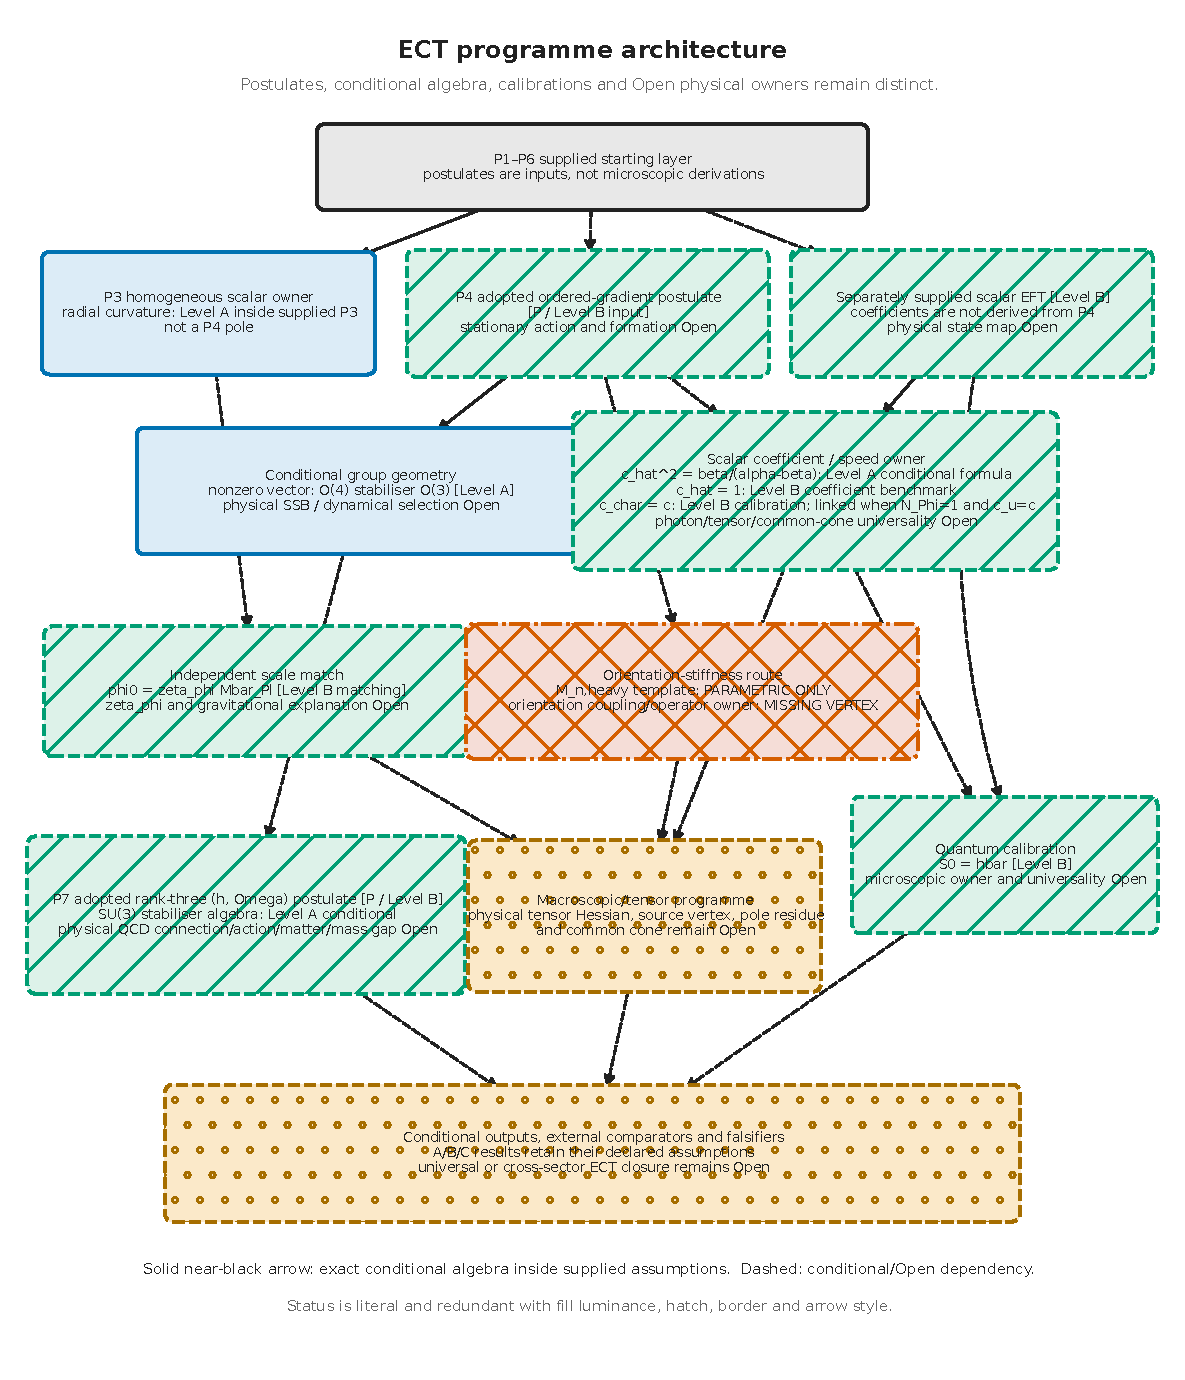
\includegraphics[width=\textwidth,height=0.70\textheight,keepaspectratio]{figures/r177/global/fig_ect_architecture_r177.pdf}
\caption{Schematic programme map of Euclidean Condensate Theory.
P4 adopts the physically relevant nonzero-gradient branch and supplies
its analysis chart (Level-B structural input); its stabiliser is $O(3)$
(Level-A conditional group theory).  A stationary owner, stability domain and
spontaneous formation/selection are not derived.  The scalar
characteristic theory is then separated from proposed macroscopic/tensor and
coherent/quantum completions.  The present action does not derive a common
physical gravity--quantum backreaction vertex, so the two boxes organise
targets rather than consequences of one closed action.  Every arrow is a
dependency or candidate route whose status is controlled by the main text
and status tables.
The benchmark identification $\alpha=2\beta$ used elsewhere in the paper
is not the generic branching condition; the full scalar-principal condition is
$\beta(\beta-\alpha)<0$; on the declared healthy $\beta>0$ branch this
is $\alpha>\beta>0$.}
\label{fig:ect_architecture}
\end{figure}

ECT proposes a deeper Euclidean-medium programme rather than merely an
interpretation of known quantum equations.  What is presently established is
more limited: selected Gaussian/coherent constructions reproduce standard
mathematical structures after additional premises are supplied.  The origin
of probability, outcomes, the physical operator algebra, universal
$\hbar$, and the quantum--classical transition remains Open.  Likewise the
physical tensor/gravity sector is not generated by the scalar action.  Figure
\ref{fig:ect_architecture} is therefore a navigation map: Parts~II and~III
develop separate completion programmes whose common microscopic owner and
backreaction remain to be derived.

This difference is reflected already at the level of the equations to be
solved. Standard quantum mechanics is formulated as an initial-value
theory for a wavefunction, for example
\[
i\hbar\,\partial_t\psi = H\psi,
\]
where $\psi(\mathbf x,t)$ is a probability amplitude and
$|\psi(\mathbf x,t)|^2$ is interpreted statistically through the Born
rule. ECT begins instead from a Euclidean field equation of the form
\[
\delta^{AB}\partial_A\partial_B\Phi - V'(\Phi)=0,
\]
whose solution $\Phi(X)$ is interpreted as a physical condensate
configuration in a four-dimensional Euclidean arena. The fundamental
problem is therefore a boundary-value problem rather than a Cauchy
evolution problem: boundary data specify a Euclidean boundary-value problem
rather than initial data propagated only forward in time.  They fix one
solution only after existence, uniqueness and stability/well-posedness have
been established for the stated nonlinear equation, domain and boundary
class; these global properties remain Open for ECT.
In this framework probability is not postulated at the bare Euclidean level,
but coarse-graining or decoherence alone does not create a probability
measure or select an outcome.  Those ingredients require an independently
derived state, measure and update rule and remain Open.

The resulting hierarchy is one of the central structural outputs of ECT.
At the most fundamental level one has the Euclidean condensate equation.
In the ordered broken phase this reduces to an effective equation with
kinetic tensor
\[
K^{AB}=\beta\,\delta^{AB}-\alpha\,n^A n^B,
\]
whose retained-component Lorentzian admissibility requires
$\alpha>\beta>0$.  Writing the
ordered direction as the common-length coordinate $x^0=w$ gives the
hyperbolic Klein--Gordon operator.  This is not yet an identification of
$w$ with a reading in seconds: the physical clock requires the
state-dependent congruence/lapse map of
Eq.~\eqref{eq:ect_external_depth_lapse_map} and a dimensional calibration.
After a positive-frequency/state choice, complex envelope, operator map and
$S_0$ normalisation are supplied, a non-relativistic
Schr\"odinger-type equation can be recovered conditionally.  This is a
Level-B/Open reduction, not yet a unique descendant of P1--P6.

\paragraph{Terminological note.}
The terms ``dark matter'' and ``dark energy'' are retained as names for
observational phenomena and standard comparison sectors.  The Level-C HRC data diagnostic uses no particle-halo term, but this does not derive
the fit from ECT, exclude particle dark matter, or determine ECT ontology.
The late-time background closure is separate and has its own declared
status.  Fundamental particle content and the cosmological fraction budget
remain Open.

Throughout this paper we distinguish four status classes:
Level~A results derived inside stated assumptions; Level~B conditional
structures with declared missing matching inputs; Level~C phenomenological
fits, external benchmarks or supplied application models; and Open questions
for which the required owner has not been derived or identified.
A summary is given in Table~\ref{tab:ect-levels}.

The paper is organised into five parts.

\textbf{Part~I (Foundations)} develops the ordered-branch effective
theory of the condensate and the conditional Lorentzian classification of
one supplied scalar principal tensor.  It records one scalar characteristic
cone and conditional matchings for
$c_{\rm char}$, $G_N$ and~$S_0$; physical Dirac/CAR, gauge and tensor owners
remain Open.
It also inventories candidate gauge/matter completion routes and
preferred-direction operators; their local bundles, representations,
coefficients and observable maps remain Open.
The neutrino section inventories supplied seesaw/Weinberg benchmarks; no
physical chirality, sterile state, mass operator, PMNS matrix or
Dirac/Majorana preference is derived.

\textbf{Part~II (Macroscopic Physics)} develops the macroscopic branch
and a scalar--tensor closure whose metric and scalar equations follow from
the displayed Level-B ansatz.  It studies cosmological and galactic
phenomenology at their separately declared closure levels.  The ordered
branch also permits candidate anisotropic tensor structures, but the present
field equation contains no orientation stress.  Such a stress and any
lensing, growth, or cluster observable attributed to it remain Open pending
a covariant $S_n[g,n]$, constraints, variation, on-shell identity, and
physical projection.

\textbf{Part~III (Quantum Sector)} develops the coherent quantum
branch: a conditional Osterwalder--Schrader Hilbert-space reconstruction,
with reflection positivity as one required hypothesis, canonical
structure, exchange topology, decoherence, and the Principle of
Euclidean Stationarity.  In this sector ECT aims to show that large
parts of quantum formalism appear as effective ordered-branch
structures rather than primitive postulates.  Inside a separately supplied
local first-order fermionic/CAR effective theory, a smooth strictly positive
temporal kinetic factor can be removed by an invertible canonical
normalisation; this conditionally excludes Pauli violation generated solely
by that factor.  The physical ECT fermion, CAR and spin--statistics owners,
as well as the Born measure, measurement update and unique-outcome mechanism,
remain Open.
Part~III is further extended by a dedicated upgrade layer on the
gravity--matter interface: a reduced-state reformulation of the
hybrid-consistency problem; an architectural operational criterion
for gravity-induced-entanglement experiments; a bounded mediator-channel audit
of the enumerated candidate class, in which the tested fixed-$\alpha,\beta$
tangent-director linear route has a missing vertex and the full gravitational
mediator is not identifiable; an infrared section retaining BMS, memory and
soft gravitons only as external completion tests; and a
structural mapping of the critical-shell black-hole picture onto
the modern islands and quantum-extremal-surface language, together
with a compact cross-programme diagnostic summary.

\textbf{Part~IV (Reverse Analysis, the P7 $SU(3)$ Structural
Postulate, and Physical-Colour Constraints)} is a conditional completion
programme above the forward work of Parts~I--III.  It records P7 as an adopted
Level-B global rank-three bundle with $(h,\Omega)$; the resulting $SU(3)$
frame group is Level-A mathematics conditional on that postulate.  It does not derive a physical colour bundle, connection, action,
matter representation or spectrum.  The exact scoped results are the
stabiliser of a nonzero fundamental vector and the absence of an injective
$\mathfrak{su}(3)\hookrightarrow\mathfrak{so}(4)$ embedding; reducible,
emergent/nonlinear and kernel-bundle routes remain admissible.  The part then
displays one leading colour-EFT truncation, restates standard anomaly
conditions, and inventories every physical owner as conditional or Open.
No framework choice about the Clay continuum object is promoted to a Level-A
ontology or theorem about nature.

\textbf{Part~V (Summary, Comparisons, and Outlook)} consolidates the
framework through its constants map, completion tests, failure gates, open problems, and
the derivational summary of structures usually treated as independent
postulates or empirical inputs in standard physics.  It keeps the standard
conditional gauge-normalisation identities separate from the Open
ECT-specific gauge/matter construction.

The four claim levels defined above govern the verbs used throughout the
preprint: \emph{derived} refers to exact mathematics in the declared model and
assumptions with an explicit reproducible derivation; checks verify but do not
replace it;
\emph{conditional} retains its supplied assumptions; \emph{phenomenological}
marks matching or stress testing; and \emph{Open} marks a missing physical
owner.  This is part of the scientific claim, not a separate review ledger.

Later sections keep the detailed sector diagnostics with their owning
derivations.  Section~\ref{sec:quantum_vacuum} treats Casimir, Rindler/KMS and
particle-production calculations as external targets for a future ECT vacuum
completion, not as limits already derived from one ECT correlator.  The
galactic programme in Section~\ref{sec:mp_galactic} and
Appendix~\ref{app:lof_full_derivation} records two negative scalar routes and
then studies a separately supplied HRC closure.  Its scalar coupling,
stationary-response equation, conditional baryonic Tully--Fisher algebra and
exploratory environment law are derived or defined in those owning sections;
the physical coordinate map, gravity bridge, extended-body response and the
origin, sign and amplitude of any environment dependence remain Open.

The present formulation should be understood primarily as an effective
low-energy description of condensate excitations.  The analysis focuses
on long-wavelength perturbations around the supplied ordered-sector chart.  A
supplied $\alpha>\beta>0$ scalar principal tensor then has Lorentzian
characteristics; promotion of that scalar cone to the physical clock,
metric and cross-sector causal structure remains Open.  The microscopic
dynamics of the condensate at very high energies is also Open.

Later sections separate exact conditional calculations, external source
models, data diagnostics and Open observable maps.  These inventories test
what an owner-complete ECT calculation would require; they are not evidence
that condensate dynamics is already connected to the cited phenomena.%
\footnote{A shorter companion article providing an accessible overview
of the main ideas, results, and open problems of ECT is available
at \url{https://doi.org/10.5281/zenodo.19430795}.}

% ============================================================

%==============================================================
\clearpage
\part{Foundations: Postulates, Symmetry Breaking, and Emergent Laws}
\label{part:foundations}
%==============================================================

% SECTION 2: POSTULATES OF ECT — NEW VERSION (5 postulates)
% ============================================================
\section{Postulates of Euclidean Condensate Theory}
\label{sec:postulates}

\textit{This section states the foundational symmetry and condensate
postulates of ECT.
It establishes the minimal bare framework from which later
Level~A/B/C results are developed; it is not itself a
phenomenological or EFT-derivation section.}

Euclidean Condensate Theory (ECT) starts not from already formed
spacetime, matter, or energy in their familiar late-physics sense,
but from a more primitive Euclidean $\Phi$-medium.
The role of the foundational postulates is not to impose
the observed macroscopic world by hand, but to formalise the minimal
structural properties that such a medium must possess if causal
structure, geometry, and gravitational dynamics are to emerge from it.

The foundational construction is organised in three levels.
First, the ontological properties of the $\Phi$-medium are stated
explicitly (Section~\ref{subsec:phi_medium_properties}).
Second, the working postulates P1--P6 specify the concrete ECT
realisation of that medium.
Third, supplied effective branch rules such as BR1 define special coherent
analysis sectors on the ordered chart.  The manuscript then investigates a
geometric macroscopic sector and a coherent sector; their common microscopic
descent from one physical condensate state remains Open.
The smooth coherent sector is not introduced as a fundamental postulate.
It is a supplied effective branch closure: once a smooth non-vanishing
single-valued complex collective field is admitted, integer winding is a
topological theorem.  P3 plus P4 do not themselves derive that complex
field, its stiffness or the action normalisation~$S_0$.
The later analysis of kinetic tensors and signature classes, including the
healthy Lorentzian component~(Section~\ref{sec:metric_classification}), is likewise
not an extra postulate but a conditional principal-symbol analysis on
the supplied chart.
Subsequent sections distinguish exact consequences of stated premises from
supplied effective completions, phenomenological benchmarks and Open physical
maps; they do not all follow from P1--P6.

\subsection{Glossary of terms}
\label{subsec:glossary}

Before stating the postulates we fix the meaning of terms that
in the literature are sometimes used interchangeably but carry
distinct meanings in ECT.

\medskip
\noindent\textbf{Field~$\Phi$} --- the unique fundamental
microscopic degree of freedom: a real scalar defined on~$\mathcal{M}^4$.

\medskip
\noindent\textbf{Vacuum} --- a stationary, physically admissible
background branch of the fundamental $\Phi$-medium.  P3 owns only its
homogeneous stationary minima.  P4 independently adopts a physically relevant
nonzero-gradient sector; the completed stationary action, state and
boundary/domain problem realising that postulate remain Open.

\medskip
\noindent\textbf{Condensate} --- shorthand for the adopted P4 ordered-sector
description of the $\Phi$-medium, here characterised by
$\langle\partial_A\Phi\rangle \neq 0$.  It is not an additional object; its
stationary action/state/domain owner and formation history remain Open.

\medskip
\noindent\textbf{Order parameter} --- a supplied collective infrared variable
of the BR1 coherent-sector closure,
$\Phi_{\rm eff} = \rho\,e^{i\theta}$,
used to describe candidate low-energy excitations on the ordered chart.
It is introduced only at the effective level; neither its descent from the
bare micro-action nor physical symmetry breaking is established.

\medskip
\noindent\textbf{Orientation variable~$n_A$} --- a collective coordinate
on the supplied nonzero-gradient chart describing its local direction.
It does not appear as an independent field in the bare micro-action, and its
physical state/action owner remains Open.

\medskip
\noindent\textbf{Electroweak bookkeeping field~$\Phi_{\rm ew}$ and
canonical doublet~$H$} --- the embedded low-energy scalar variables of the
secondary electroweak sector, related by
$H\equiv\Phi_{\rm ew}/\sqrt{2}$.  The field $H$, not
$\Phi_{\rm ew}$, is used in canonically normalised Yukawa operators.  Both
are distinct from the fundamental bare condensate field~$\Phi$ of~P3 and
appear only in the electroweak-like embedding
(Section~\ref{sec:ew_embedding}).


\subsection{Ontological properties of the \texorpdfstring{$\Phi$}{Phi}-medium}
\label{subsec:phi_medium_properties}

The $\Phi$-medium is a pre-physical entity: it exists prior to
spacetime, quantum mechanics, and any emergent physics.
Its description must therefore not rely on the language of energy,
quantum fluctuations, or effective Lagrangians.
The following structural properties characterise the $\Phi$-medium
in purely geometric and configurational terms, prior to any ordering
or symmetry breaking.

\paragraph{Layer~S\,: Properties of the medium.}

\begin{description}
  \item[\textbf{S1} --- Connected Euclidean carrier.]
    The $\Phi$-medium exists on a connected four-dimensional Euclidean
    carrier $\mathcal{M}^4$ with a flat Euclidean metric.

  \item[\textbf{S2} --- Directional isotropy.]
    Prior to ordering, all four directions on $\mathcal{M}^4$ are
    equivalent: the medium is $O(4)$-isotropic.

  \item[\textbf{S3} --- Point homogeneity.]
    Prior to ordering, all points of $\mathcal{M}^4$ are equivalent;
    ordering may break this homogeneity locally.

  \item[\textbf{S4} --- Regularity.]
    Configurations $\Phi(X)$ are locally regular where they contain no
    defect cores; configurations with localised defect cores on
    submanifolds of lower dimension are admissible.

  \item[\textbf{S5} --- Locality.]
    The local state of the $\Phi$-medium at $X$ is determined by the
    local configuration in a neighbourhood of~$X$, not by non-local
    rules on all of~$\mathcal{M}^4$.

  \item[\textbf{S6} --- Multiplicity of configurations.]
    The configuration space is non-trivial: no configuration is
    privileged a priori; globally and locally distinct configurations
    are admissible.

  \item[\textbf{S7} --- Adopted ordered sector.]
    ECT adopts through P4 a physically relevant ordered-gradient sector with
    $\langle\partial_A\Phi\rangle\neq0$.  The complete stationary action,
    state, stability domain, physical transition and dynamical selection
    mechanism realising this input are not supplied.

  \item[\textbf{S8} --- Deformability and relational response.]
    A regular ordered configuration can respond through local deformation
    and reconfiguration.  Physical distinctions are encoded by invariant
    strains, gradients, defects, holonomies and response to boundary or
    material probes, rather than by a passive relabelling of the same
    configuration.  S8 does not identify arbitrary pointwise changes of the
    compact phase or spacetime director as gauge redundancies; a local bundle
    and its quotient must be supplied separately.

  \item[\textbf{S9} --- Inhomogeneity of ordering.]
    Ordering need not be globally uniform; ordered domains, transition
    zones, and local deviations from a uniform background are admissible.

  \item[\textbf{S10} --- Topological completeness.]
    Once a physical configuration space, target, boundary class and action
    are supplied, all compatible topological sectors are admitted rather
    than excluded a priori.  S10 does not identify the abstract P4 orbit
    with the complete physical vacuum manifold.

  \item[\textbf{S11a (conditional theorem)} --- Infinitesimal local deformability.]
    Subject to fixed admissible boundary data, regularity and a fixed
    topological sector, a locally regular configuration admits sufficiently
    small compactly supported deformations.  This is the tangent-space
    structure of the regular scalar configuration space, not a new dynamical
    postulate.

  \item[\textbf{S11b (candidate)} --- Finite branch reconfigurability.]
    Some ordered branches may be connected by finite-action admissible
    transition configurations.  Changing the topological sector still
    requires an allowed defect or transition configuration.  Path existence
    does not imply that the dynamics traverses the path, overcomes a barrier,
    or relaxes reversibly.  S11b contains no relaxation law, channel spectrum
    or gravitational response.

\end{description}

\paragraph{Layer~DP\,: Dynamical principle.}

\begin{description}
  \item[\textbf{DP} --- Variational stationarity.]
    Physically realisable configurations satisfy the stationarity condition
    for a local
    functional $S_E[\Phi]$ compatible with the basic symmetries of the
    medium, and satisfy conditions ensuring the well-posedness of the
    variational problem.  Stationarity supplies equations of motion but does
    not choose one extremum/history, establish stability, assign a
    probability, or provide an outcome/record-selection rule.
\end{description}

\medskip
The working postulates P1--P6 of ECT constitute the present concrete
realisation of this framework within the minimal real-scalar field theory.
They are adopted defining inputs, denoted $[P]$; a postulate is not demoted to
Open merely because it is not derived from an earlier postulate.  Open status
instead attaches to a missing constructive owner, state/selection mechanism,
microscopic descent or observable map.  A theorem derived from named inputs is
Level~A conditional on them; an adopted physical matching or structural
closure is Level~B; a fit, toy or benchmark is Level~C.  In that realisation:
P1 makes explicit S1--S3;
P2 formalises S2 at the level of the bare symmetry;
P3 realises S4, S5, and provides the minimal local variational
realisation associated with DP;
P4 supplies the S7 ordered-gradient datum;
P5 realises S8;
P6 makes explicit S6 and S9.
The broader topological completeness property S10 is partially reflected,
within the supplied smooth coherent branch, by the conditional winding
classification of~BR1.
S11a is conditional configuration-space mathematics following from the
regular scalar field space once its boundary and topology guards are stated.
S11b is a candidate structural property: finite branch reconfigurability has
not been derived from the frozen minimal P1--P6 action.  Its narrower
threshold-relaxation specialisation is a further independent constitutive
extension.  Any branch-EFT hypothesis about a localised carrier, its action
cost or its elastic coefficients belongs to a later post-order constitutive
layer, not to this pre-physical property list.  Such a hypothesis cannot
follow from deformability alone and is not inserted into the minimal P1--P6
action by this classification.
The deformability/relational-response property S8 is realised by the working
postulate~P5, which is logically independent of P1--P4 and P6.  It asserts
that the ordered branch is a responsive medium whose physical state is read
through invariant deformation and relational observables.  It does not
promote a global symmetry or the physical director to a local gauge orbit.
Together, P1--P6, the additional effective closure BR1, and DP provide
the present layered structural framework of ECT.

\subsection{List of postulates}
\label{subsec:postulate_list}

\medskip
\noindent\textbf{P1 --- Four-dimensional Euclidean arena.}
The fundamental arena is a connected four-dimensional flat Euclidean
carrier $\mathcal{M}^4$ with metric
\begin{equation}
  \label{eq:P1_metric}
  ds^2_E = \delta_{AB}\,dX^A\,dX^B,\qquad A,B\in\{1,2,3,4\}.
\end{equation}
The local theory is formulated in flat charts.  Whenever global equivalence
of points and the full Euclidean group are used, P1 additionally adopts the
homogeneous boundary/topology class (the canonical choice is
$\mathcal M^4\simeq\mathbb R^4$); a generic flat quotient or a manifold with a
boundary would not have that global symmetry.  No direction is distinguished
and no time coordinate is fundamental.

\medskip
\noindent\textbf{P2 --- $O(4)$-invariant action.}
The fundamental action is invariant under global $O(4)$ rotations:
\begin{equation}
  \label{eq:P2_symmetry}
  S_E[\Phi] = S_E[\Lambda\cdot\Phi], \qquad \Lambda\in O(4),
  \qquad (\Lambda\!\cdot\!\Phi)(X):=\Phi(\Lambda^{-1}X),
\end{equation}
where $\Phi$ denotes the fundamental microscopic field of the minimal
scalar realisation developed in this work.  On the homogeneous flat carrier,
translation invariance follows separately from the absence of explicit
$X$-dependence; together translations and rotations form
$E(4)=\mathbb R^4\rtimes O(4)$.  Thus $O(4)$ is the linear isotropy group, not
the full isometry group.
In possible future extensions with additional microscopic fields,
P2 should be understood as the corresponding $O(4)$-covariance
requirement on the full microscopic action.
This expresses the equivalence of all four directions in the
unbroken phase.

\medskip
\noindent\textbf{P3 --- Minimal homogeneous scalar sector.}
\label{eq:P3}
The following local real-scalar model is a deliberately minimal supplied
sector on $\mathcal M^4$:
\begin{equation}
  \label{eq:ECT_action}
  \mathcal I_E^{\rm P3}[\Phi]
  := \int d^4X\!\left\{
    \frac{1}{2}(\partial_A\Phi)^2 + V(\Phi)
  \right\},
  \qquad
  S_E^{{\rm P3},{\rm phys}}[\Phi]
  :=A_{\rm P3}\mathcal I_E^{\rm P3}[\Phi],
  \qquad A_{\rm P3}>0,
\end{equation}
\begin{equation}
  V(\Phi) = -\frac{\mu^2}{2}\Phi^2 + \frac{\lambda}{4}\Phi^4,
  \qquad \mu^2>0,\quad\lambda>0.
  \label{eq:P3_potential_two_owner}
\end{equation}
In the printed natural-unit mass convention the integral
$\mathcal I_E^{\rm P3}$ is dimensionless.  The independent constant
$A_{\rm P3}$ restores a physical-action normalisation; it is not supplied by
the displayed integral.  A Euclidean path-integral measure needs a second
positive owner,
\begin{equation}
 d\mu_{\rm P3}[\Phi]\propto\mathcal D\Phi\,
 \exp[-\kappa_{\rm P3}\mathcal I_E^{\rm P3}[\Phi]]
 =\mathcal D\Phi\,
 \exp\!\left[-\frac{S_E^{{\rm P3},{\rm phys}}[\Phi]}
                    {\Sigma_{\rm PI,P3}}\right],
 \qquad
 \kappa_{\rm P3}:=\frac{A_{\rm P3}}{\Sigma_{\rm PI,P3}}>0 .
 \label{eq:P3_measure_two_owner}
\end{equation}
Here $\Sigma_{\rm PI,P3}>0$ has action dimension and controls the measure
relative to the classical action prefactor.  Setting the same symbol in both
places would force $\kappa_{\rm P3}=1$ and would erase rather than derive the
fluctuation strength.  Neither $A_{\rm P3}$, $\Sigma_{\rm PI,P3}$,
$\kappa_{\rm P3}$ nor a relation to $\Sigma_\theta$,
$\Sigma_\vartheta$, $S_0$ or $\hbar$ is derived.  For constant
$A_{\rm P3}>0$, $\delta S_E^{{\rm P3},{\rm phys}}=0$ iff
$\delta\mathcal I_E^{\rm P3}=0$; the stationary set therefore survives the
correction, while the measure and fluctuation amplitudes remain separate
inputs.  If $\mathcal K_{\rm P3}$ is the Hessian of the reduced functional at
a supplied stable saddle, the Gaussian covariance is
$(\kappa_{\rm P3}\mathcal K_{\rm P3})^{-1}$ and the formal one-loop factor is
$\det(\kappa_{\rm P3}\mathcal K_{\rm P3})^{-1/2}$, subject to the contour,
zero/negative modes, domain, measure and regularisation.  The printed
symmetric quartic has exactly degenerate minima
$\Phi=\pm\mu/\sqrt\lambda$, hence no false-vacuum energy splitting.  It owns
a domain-wall sector but, by itself, no finite false-vacuum bounce: in the
standard thin-wall bookkeeping a supplied bias $\epsilon=\Delta V>0$ and
wall tension $\sigma>0$ give
$R=3\sigma/\epsilon$ and
$B=27\pi^2\sigma^4/(2\epsilon^3)$; both diverge as
$\epsilon\to0^+$.  A finite P3 decay saddle would
therefore require an explicitly supplied bias/deformation, finite boundary or
protocol, or another channel.  Only for such a named completion is a positive
vacuum-subtracted difference weighted by
$\exp[-\kappa_{\rm P3}\Delta\mathcal I_E^{\rm P3}]$; genuine real suppression
requires $\Delta\mathcal I_E^{\rm P3}>0$.  These measure statements identify
only $\kappa_{\rm P3}$ once the normalisation of $\mathcal I_E^{\rm P3}$ is
fixed, not $A_{\rm P3}$ and $\Sigma_{\rm PI,P3}$ separately.
It owns the classical homogeneous P3 stationary minima, their Gaussian
curvature and the on-shell Noether identities of this model.  It is not the
full DP action for the P4 gradient datum.  The action and two-well potential
are invariant under the internal reflection $\Phi\mapsto-\Phi$ and have two
classical minima exchanged by that symmetry.  Selecting one physical quantum
vacuum and spontaneous $\mathbb Z_2$ breaking require a state and the
appropriate infinite-volume or boundary/source limit; they are not asserted
here.  P3 creates neither a continuous vacuum manifold, compact coherent
phase nor stationary nonzero-gradient branch.
Gradient-sensitive $P(X)$ or other completion terms may be investigated, but
none is presently adopted as the full owner (OP-grad).

\medskip
\noindent\textbf{P4 --- Adopted ordered-gradient structural postulate.}
\label{eq:P4}
ECT postulates that its physically relevant sector is an ordered-gradient
branch with
\begin{equation}
  \label{eq:gradient_condensate}
  \langle\partial_A\Phi\rangle = u_0\,\delta_{Aw},
  \qquad u_0>0 .
\end{equation}
A convenient integrable representative is
\begin{equation}
  \label{eq:background}
  \Phi_{\rm bg}(X)=u_0w+\Phi_*,\qquad \Phi_*=\mathrm{const}.
\end{equation}
P4 is a foundational structural input $[P]$ (Level-B input in the claim
ledger), not a stationary solution derived from the displayed P3 scalar
action.  Conditional on the nonzero vector, its stabiliser under $O(4)$ is
exactly $O(3)$ (Level-A mathematics).  The representative profile is not
stationary for $\mathcal I_E^{\rm P3}$, equivalently for
$S_E^{{\rm P3},{\rm phys}}$ with constant $A_{\rm P3}>0$.  A complete
$O(4)$-invariant stationary action, state, constrained stability domain,
physical transition and dynamical formation/selection mechanism realising P4
remain Open.  Subsequent ``ordered branch'', ``broken-phase'' and ``gradient
condensate'' language refers to the adopted P4 sector; it does not claim that
P3 derives its formation history.

P3 and P4 introduce independent quantities:
\renewcommand{\arraystretch}{1.3}
\begin{longtable}{@{}L{4.8cm}L{4.8cm}L{4.8cm}@{}}
\toprule
Symbol & Definition & Level \\
\midrule
\endfirsthead
\toprule
Symbol & Definition & Level \\
\midrule
\endhead
\bottomrule
\endfoot
$\phi_0=\sqrt{\mu^2/\lambda}$ & homogeneous minimum of the supplied P3
potential & P3 conditional \\
$u_0=|\langle\partial_A\Phi\rangle|$ & magnitude of the supplied P4
gradient datum & P4 structural input \\
\bottomrule
\end{longtable}
Their dynamical relation and the complete stationary owner that realises
the adopted P4 postulate remain missing (OP-grad).

\medskip
\noindent\textbf{BR1 --- Smooth coherent topological sector (supplied effective closure; hereafter referred to simply as the coherent branch).}
\label{sec:BR1_coherent_sector}
In a smooth infrared coherent sector appended to the real-scalar P3--P4
model, low-energy excitations are assumed to admit a collective
description through
an effective order parameter
\[
\Phi_{\rm eff}=\rho\,e^{i\theta},
\qquad \rho>0.
\]
If $\Phi_{\rm eff}$ is single-valued on a closed contour
$\mathcal{C}$ that does not intersect a defect core, then the phase
defines a map $\mathcal{C}\to S^1$, and therefore the winding number
is necessarily integer:
\begin{equation}
  \label{eq:winding_condition}
  \oint_{\mathcal{C}}\partial_A\theta\,dX^A = 2\pi n,
  \qquad n\in\mathbb{Z}.
\end{equation}
Thus integer winding is a topological consequence \emph{conditional on}
the supplied non-vanishing complex order parameter.  The existence of
that compact phase sector is not derived from the bare real scalar P3.

Configurations with zeros of $\rho$, discontinuities of $n_A$,
or other non-smooth field profiles are not excluded by the full theory;
however, within the supplied orientation target
$O(4)/O(3)\simeq S^3$ they do not carry $\pi_0$-, $\pi_1$- or
$\pi_2$-protection
(Section~\ref{sec:predicted_states}).
This $S^3$ target treats $n_A$ as a polar vector, so $n_A$ and $-n_A$ are
distinct.  If a future physical completion instead identifies a headless
director $n_A\sim-n_A$, its target is the quotient $\mathbb{RP}^3$ and the
homotopy inventory must be recomputed; P4 does not choose that quotient.
Their status must therefore be analysed dynamically rather than inferred
from topology alone.
This is consistent with the broader topological completeness property~S10
of the $\Phi$-medium.  The physical target, admissible exact-gradient
configurations, boundary class, action and transition owner remain Open.

Within a supplied fixed-core compact-phase EFT, the elementary coherent-loop
representative is defined by
\begin{equation}
  \label{eq:Sloop_min}
  \iota_{\rm elem}^{\rm(fixed\ core)}=2\pi \iota_0^{\rm EFT}.
\end{equation}
The equality is a definition/evaluation at the supplied characteristic core
scale~(Section~\ref{sec:hbar_status}), not a topological derivation of a
nonzero global minimum.  A distinct optional positive-tension 1D model has
the conditional minimum $\mathcal I_{1,\min}=2\pi \iota_{0,\rm bal}^{\rm eff}$.  Neither
coefficient is automatically the operational $S_0$.  In the bending-free
elementary branch, the motivated matching chain
$\Sigma_\theta\,\iota_{0,\rm bal}^{\rm eff}\to S_0\leftrightarrow\hbar$ would imply
$\Sigma_\theta\,\mathcal I_{1,\min}=2\pi\hbar=h_{\rm P}$; the owner arrow remains Open and the
$S_0=\hbar$ arrow is an explicit Level~B calibration rather than a
derivation of the measured action constant.


\medskip
\noindent\textbf{P5 --- Deformability and relational response of the ordered branch.}
\label{eq:P5}
The ordered $\Phi$-medium is deformable and reconfigurable: neighbouring
regular configurations can be distinguished operationally by invariant
strain, gradient, defect, holonomy and response data relative to material or
boundary probes.  A passive relabelling of one configuration does not create
a new physical state.

This statement does not equate a passive relabelling with an arbitrary local
field change.  The compact phase has a global shift redundancy only when its
supplied action has that symmetry; a transformation
$\theta(X)\to\theta(X)+\alpha(X)$ is a local gauge redundancy only after a
bundle, connection and quotient have been supplied.  The director
$n_A=\partial_A\Phi/|\partial\Phi|$ is a constrained carrier-space orientation and
can be observable relative to matter or another field; $n_A(X)\to
R_A{}^B(X)n_B(X)$ is not a gauge orbit of the minimal scalar theory.

This postulate realises property~S8 of the $\Phi$-medium within the concrete
ordered-branch framework of ECT.  It is logically independent of P1--P4 and
P6: symmetry, locality and branch existence do not by themselves specify the
constitutive response of a deformable continuum medium.

P5 is motivated by the ordinary behaviour of media: a crystal responds to
strain, a superfluid to phase differences and circulation, and a liquid
crystal to director distortions relative to boundaries and probes.  In each
case response and deformation are physical, while a passive change of labels
is not.  The precise variables and symmetries differ between these systems;
the analogy therefore motivates medium character but does not manufacture a
gauge field.

\emph{What P5 does not assert.}
P5 does not exclude nonlocal observables such as winding numbers or, after a
local bundle has been supplied, holonomies and Wilson-loop data.
P5 does not by itself determine the gauge coupling constants or the
fermion representation content, and it does not derive a physical $SU(3)$ colour connection, action or
matter map. The inequality $\dim\mathfrak{su}(3)>
\dim\mathfrak{so}(4)$ excludes only a direct injective
Lie-subalgebra/residual-factor embedding in the displayed minimal
algebra. Emergent/nonlinear, reducible/singlet, independently derived bundle
and defect-kernel routes are not excluded; P7 is the adopted Level-B
structural completion used in this manuscript, not a theorem that it is the
necessary or unique microscopic origin of physical colour.

\emph{Gauge-completion programme.}
P5 motivates asking which coordinate descriptions become redundant after
reduction, but it does not make the physical spacetime director $n_A(X)$ a
gauge orbit or localise a global compact phase.  The exact inputs presently
available are global compact-phase algebra in a supplied BR1 sector and the
Lie-algebra identity $\mathfrak{so}(3)\cong\mathfrak{su}(2)$.  Local bundles,
connections, gauge-volume quotients, physical state spaces and a chiral
$SU(2)_L\times U(1)_Y$ identification remain Open completion data; see
Sections~\ref{sec:u1_emergence} and~\ref{sec:nonabelian_embedding}.


\medskip
\noindent\textbf{P6 --- Multiplicity of configurations and admissibility of non-uniform ordering.}
\label{eq:P6}
The configuration space of the $\Phi$-medium is non-trivial: no single
configuration is singled out a priori as the unique physical realisation~(S6).
In particular, P6 admits spatially varying backgrounds, domain
structures and transition configurations in the ordered-sector configuration
space~(S9).  Their stationarity, physical occurrence, profiles and dynamics
are not fixed by this admissibility postulate and remain Open.
This postulate does not prescribe the magnitude or functional form of
such inhomogeneities; it states only that the ECT framework is not
restricted to a single homogeneous ordered configuration.

\subsection{Operational principle of relationality}
\label{subsec:relational}

In the absence of a fundamental time coordinate, as specified by the
arena~P1, the relational approach provides a natural and operationally
consistent way to define observables: physical observables are ratios
between physical subsystems. This is motivated by P1 but does not
follow from it as a theorem.

\subsection{Independence of postulates}
\label{subsec:independence}

The six working postulates P1--P6 are logically independent.
In particular, the medium-character postulate~P5 is independent of
P1--P4 and P6: it cannot be derived from action symmetry, locality,
field content, ordering, or configuration multiplicity alone.
\begin{itemize}
  \item P1 does not follow from P2--P6: neither $O(4)$ invariance, nor
    the choice of field content, nor the admissibility of an ordered
    branch, nor the multiplicity of admissible configurations fixes the
    existence of a connected four-dimensional Euclidean arena.
  \item P2 does not follow from P1 and P3--P6: the existence of a
    Euclidean carrier, a local scalar field, an ordered branch, and a
    non-trivial configuration space does not by itself enforce global
    $O(4)$ invariance of the bare description.
  \item P3 does not follow from P1, P2, P4, and P6: the specific
    real-scalar field content and the minimal local micro-action must be
    stated separately.
  \item P4 does not follow from P1--P3 and P6: its nonzero ordered-gradient
    datum is an additional supplied EFT input beyond the minimal bare
    micro-action and the mere admissibility of non-trivial or non-uniform
    configurations.  Physical realisation and selection remain Open.
  \item P6 does not follow from P1--P4: the non-triviality of the
    configuration space and the admissibility of inhomogeneous ordering
    are additional structural properties not entailed by the minimal
    scalar micro-action or the ordered branch specification alone.
\end{itemize}

BR1 is an adopted Level-B effective closure, not a P1--P6 theorem: it
supplies a nonvanishing single-valued complex collective field on its declared
infrared domain.  Given that input and a closed contour avoiding zeros, integer
winding is a Level-A topological consequence.  Microscopic descent, formation
and selection of the BR1 domain remain Open.

\subsection{Discussion of the postulates}
\label{sec:postulates_discussion}

\subsubsection*{P1 --- Euclidean arena}

\paragraph{Physical meaning.}
Space and time are not co-equal primary structures of nature.
At the fundamental level there exists only a four-dimensional
geometric arena in which all directions are indistinguishable.
The notions of ``before'' and ``after'', ``spatial'' and ``temporal''
are not built into the foundation of the theory: they may emerge
from it under certain conditions, but are not postulated from the outset.

This fundamentally distinguishes ECT from all theories that start with
a Lorentzian spacetime $(-,+,+,+)$: in those theories the distinction
between time and space is encoded from the very beginning in the sign
of the metric.

\paragraph{Physical motivation.}
Euclidean geometry as a starting structure appears in physics in
several independent contexts.
In quantum field theory the Wick rotation $t\to-i\tau$
(Matsubara formalism~\cite{Matsubara1955}) can relate Lorentzian and
Euclidean correlation functions when the required analyticity, contour,
state and measure hypotheses hold; it does not automatically make every
path integral well-defined.
In the Hartle--Hawking no-boundary proposal~\cite{HartleHawking1983}
the candidate cosmological state is defined through a path integral (or
semiclassical saddles) over regular compact positive-definite or complex
four-geometries.
In instanton calculations~\cite{Belavin1975} tunnelling configurations
are solutions of Euclidean equations of motion.
These established Euclidean constructions have different mathematical and
interpretive roles and do not imply ECT's ontological postulate.  In ECT a
Euclidean scalar medium is instead proposed as physically primary.

\paragraph{On dimensionality.}
P1 adopts $d=4$.  One motivation is the exact dimension count
$\dim[O(d)/O(d-1)]=d-1$, so $d=4$ leaves three directions transverse to a
nonzero ordered vector.  Identifying those directions with all observed
physical space still requires the clock, metric and matter maps and is not a
derivation of $d=4$ from observations.  See \S\ref{sec:universe_size} for the
distinction between topological and force-law dimensionality.  The deeper
origin of the adopted dimensionality remains Open~(OP0).

\paragraph{What P1 forbids.}
Lorentzian spacetime~$\mathbb{R}^{1,3}$ is not an admissible
fundamental arena in ECT. It may arise as an effective structure,
but is not built into the foundation.

\subsubsection*{P2 --- $O(4)$-invariant action}

\paragraph{Physical meaning.}
The laws of physics in the symmetric phase are identical under any
rotation in~$\mathcal{M}^4$. No one of the four directions is
dynamically distinguished.

\paragraph{Physical motivation.}
$O(4)$ is the maximal linear group preserving the positive-definite tensor
$\delta_{AB}$; on the homogeneous flat carrier the full isometry group is
$E(4)=\mathbb R^4\rtimes O(4)$.  P2 adopts the $O(4)$ isotropy of the action,
while point homogeneity and translations are separate domain/action
statements.  A smaller linear isotropy such as $O(3)$ would explicitly single
out a direction.  The assertion that a physical state chooses an $O(3)$
stabiliser is instead P4 input, while its stationary dynamical owner and
formation remain Open.  No claim that $O(4)$ is the largest possible internal
or spacetime symmetry is needed.

\paragraph{Consequence for the effective sector.}
Within the supplied P4 chart, the nonzero vector datum defines a preferred
direction.  The most general symmetric rank-2 tensor compatible with the
residual $O(3)$-symmetry is constructed from $\delta^{AB}$ and $n^A n^B$.
Its explicit form and uniqueness are established as
Theorem~\ref{thm:tensor_uniqueness} in Section~\ref{sec:tensor_uniqueness}.

\paragraph{What P2 forbids.}
Any action that explicitly singles out one of the four directions
of~$\mathcal{M}^4$ at the P2 microdynamic level.  The present anisotropic EFT
analysis is conditioned on the direction supplied by P4; it has not been
derived as spontaneous ordering.  Any future action that owns that physical
selection must remain $O(4)$-invariant before its state and boundary limit are
specified.

\subsubsection*{P3 --- Minimal scalar microdynamics}

\paragraph{Physical meaning.}
The minimal P1--P6 dynamical sector contains one real scalar~$\Phi$.
Within that deliberately minimal sector, effective variables, collective
modes and geometric structures are constructed from this field.  The
reverse-engineered P7 extension adds an internal colour module and therefore
must not be described as part of the scalar-only microscopic basis.

\paragraph{Why a scalar.}
A single real scalar is the minimal one-component choice compatible with
P2: it carries no spacetime index and introduces no preferred direction.
This is an adopted economical field content, not a uniqueness theorem;
isotropic multiplets or additional fields are possible in named completions.

\paragraph{Form of the action.}
The action~\eqref{eq:ECT_action} at the level of P3 contains only an
isotropic kinetic term and a potential.  An independent director does not
appear in it.  The composite coordinate
$n_A=\partial_A\Phi/|\partial\Phi|$ introduces no second local degree of
freedom where $|\partial\Phi|>0$, but is singular at zero gradient and changes
the operator/constraint bookkeeping.  Treating $n_A$ as an independent
dynamical field would enlarge P3 and requires a separately supplied action.

\paragraph{On the potential.}
The double-well $\phi^4$ potential is the standard mechanism for
spontaneous $\mathbb{Z}_2$-symmetry breaking $\Phi\to-\Phi$.
Importantly, this potential does not by itself create a continuous
vacuum manifold nor generate the coherent phase structure later isolated as~BR1;
the latter belongs to the effective collective sector.
The potential specifies the minimal local microdynamics of~$\Phi$
and defines a local minimum at finite field amplitude
$\phi_0=\sqrt{\mu^2/\lambda}$ in the microscopic potential.
However, $V(\Phi)$ alone is not sufficient to produce a stationary
gradient-ordered vacuum: the nonzero-gradient analysis datum is supplied
separately by~P4.
The value $\phi_0$ is a technical characteristic of the micro-potential;
the ordered-chart quantity used downstream is the supplied gradient scale
$u_0$~(P4), whose nonzero vector has $O(3)$ stabiliser.  Its physical
realisation remains Open.

\paragraph{What P3 forbids.}
At the fundamental level: any additional fields.
There are no fundamental spinors, vectors, or tensors.
If such objects appear, they do so only as effective excitations
or collective variables at a higher level of description.

\subsubsection*{P4 --- Adopted ordered-gradient branch and its EFT chart}

\paragraph{Physical meaning.}
P4 adopts the physically relevant sector of ECT as one in which the mean
gradient is nonzero and directed along one of the four Euclidean directions.
This is a defining structural input and makes the subsequent broken-phase EFT
analysis nontrivial; it is not a theorem that the displayed P3 action owns a
stationary vacuum of that form.

\paragraph{Why the gradient is the relevant order parameter.}
The expectation value $\langle\Phi\rangle=\phi_0\neq 0$ is
$O(4)$-invariant: a scalar does not distinguish directions and therefore
does not by itself break the Euclidean symmetry.
By contrast, $\partial_A\Phi$ transforms as a vector under $O(4)$.
A non-zero expectation value
$\langle\partial_A\Phi\rangle = u_0\,\delta_{Aw}$
defines the direction~$w$ and has stabiliser $O(3)$ inside $O(4)$.
Within the present minimal single-field ECT framework,
$\partial_A\Phi$ is the lowest-canonical-dimension local \emph{polar-vector}
order parameter at first derivative order.  It can produce directional
ordering without adding a fundamental field or explicit anisotropy.  This is
not a uniqueness theorem for all one-scalar order parameters: a nematic
composite such as
$\langle\partial_A\Phi\partial_B\Phi
-\delta_{AB}(\partial\Phi)^2/4\rangle$ could select an unoriented axis while
$\langle\partial_A\Phi\rangle=0$, with a different target and stabiliser.

\paragraph{On the status of P4.}
In the minimal bare action~P3 the standard $\phi^4$ potential reaches
its minimum on homogeneous configurations with $\partial_A\Phi=0$.
Therefore P4 is not a theorem of the bare micro-action.  It is instead
the adopted structural postulate that a physically relevant ordered-gradient
sector exists.  It introduces no explicit anisotropy into P3, but P3 does not
derive its stationary action, amplitude, stability, formation or selection.
Constructing a more general $O(4)$-invariant gradient-sensitive functional
$P(X)$, $X\equiv(\partial_A\Phi)^2$, with a stable stationary branch at
$X=u_*^2>0$ is an Open foundational owner problem~(OP-grad), not a condition
for acknowledging P4 as a postulate.

\paragraph{On notation.}
The expectation values $\langle\Phi\rangle=\phi_0$ and
$|\langle\partial_A\Phi\rangle|=u_0$ have different physical meanings
and different dimensions:
$[\phi_0]=\mathrm{GeV}$ and $[u_0]=\mathrm{GeV}^2$ in natural units.
They should not be identified.
In the scale inventory of Section~\ref{sec:three_scales}, the radial
symmetry-breaking amplitude $\phi_0\sim\bar M_{\rm Pl}$ is the primary
energy-scale candidate
(Section~\ref{par:planck_scale}).

\paragraph{The orientation coordinate.}
On the supplied nonzero-gradient P4 chart, $n_A$ is the normalised local
direction, with reference map $n_A=\delta_{Aw}$.  The relation
$n_A=\partial_A\Phi/|\partial\Phi|$ is a coordinate construction only where
$|\partial\Phi|>0$; it is neither a selected physical vacuum nor a
symmetry-breaking event, and it is not a pointwise substitution in the bare
microscopic P3 action.

\subsubsection*{BR1 --- Smooth coherent topological sector}

\paragraph{Physical meaning.}
Within the chosen smooth BR1 effective sector, admissible
configurations have a globally consistent nonvanishing compact phase on the
declared contour and therefore integer winding.  This restriction defines
that supplied sector; it neither excludes defect/noncoherent sectors from the
full configuration space nor selects which sector is physically realised.

\paragraph{Origin of the order parameter.}
In the separately supplied coherent IR closure~BR1, and only within
its declared low-energy domain, collective excitations are represented by an
effective order parameter
$\Phi_{\rm eff}=\rho\,e^{i\theta}$.
This is not a fundamental variable of the displayed microdynamics but an
IR collective object introduced by the adopted Level-B closure.  Its
microscopic descent and physical selection remain Open.  The phase~$\theta$
belongs to this collective object, not to the real field~$\Phi$.

\paragraph{Topological content.}
The integer winding condition is determined by the homotopy group
$\pi_1(S^1)=\mathbb{Z}$~\cite{Nakahara2003} and is independent of
contour shape or dynamics.
The homotopy classification of the supplied orientation target
$O(4)/O(3)\simeq S^3$, including
$\pi_0=\pi_1=\pi_2=0$ and the abstract texture/skyrmion classes
$\pi_3(S^3)=\mathbb{Z}$, is developed in
Section~\ref{sec:predicted_states}.
This is Level-A mathematics conditional on that target, not yet a physical
defect or relic prediction.
Analogous conditions underlie the quantisation of circulation in
superfluid helium $\kappa=h/m$~\cite{Donnelly1991} and of magnetic
flux in superconductors $\Phi_0=h/2e$~\cite{Abrikosov1957}.
In those physical systems the circulation or flux quantum also uses a
separately owned stiffness, charge or mass normalisation; integer topology
alone does not determine its action scale.  ECT applies the same winding
classification to its separately supplied collective phase in four Euclidean
dimensions; the physical normalisation, state and action remain independently
owned.

\paragraph{What BR1 excludes from the present reduction.}
Within the coherent sector: configurations with fractional winding
numbers of the phase, with discontinuities in~$n_A$, or with zeros
of the order parameter. All three classes are mathematically
admissible within~P1--P6 but do not belong to the declared smooth BR1
reduction.  BR1 does not determine which sector is physically realised.


\subsubsection*{P5 / S8 --- Deformability and relational response}

\paragraph{Physical meaning.}
Property~S8, realised by the working postulate~P5, states that the
$\Phi$-medium is a deformable and reconfigurable continuum rather than a
rigid structure.  Its physical state is probed through invariant deformation,
defect, gradient, boundary-response and, where a bundle exists, holonomy data.
This is a constitutive statement about response.  It is not a declaration
that every pointwise field value is unobservable or that every local change is
a gauge transformation.

\paragraph{Why S8 is not a repetition of P2 or P3.}
P2 specifies a global symmetry of the bare action and P3 its locality.  S8
instead specifies the class of constitutive behaviour: admissible regular
configurations can deform, and physical readout compares their invariant
response to neighbouring configurations, matter and boundaries.  Neither a
global symmetry nor deformability alone creates a local redundancy.

For the supplied compact phase, a constant shift can be redundant when the
action depends only on derivatives.  A point-dependent shift requires an
independently supplied local bundle and connection.  The director
$n_A=\partial_A\Phi/|\partial\Phi|$ is a physical constrained orientation of
the scalar gradient, not an internal label that can be rotated arbitrarily at
each point.  Only passive coordinate/frame relabelling of the complete set of
fields is automatically redundant.

\paragraph{Consequences.}
S8 has structural implications, but it does not create a physical gauge
field:
\begin{enumerate}[label=(\roman*)]
  \item a global phase shift can identify equivalent descriptions in the
    supplied derivative-only compact-phase sector, while local phase
    covariance is an additional completion;
  \item physical director distortions, gradients and defects are observable
    relationally and must not be quotiented as local gauge directions;
  \item a connection may be introduced only after an independently
    supplied local bundle-covariance hypothesis.  Neither P5 nor S8
    supplies that connection, its action, its state or its matter
    representation;
  \item the algebraic isomorphism
    $\mathfrak{so}(3)\cong\mathfrak{su}(2)$ does not identify the
    physical chiral weak group $SU(2)_L$.  Combining the phase and
    orientation labels therefore does not derive a physical
    $SU(2)_L\times U(1)_Y$ gauge theory;
  \item a continuity equation for the coherent density
    follows only from a supplied action with the corresponding continuous
    symmetry and its Noether current; medium character alone is
    insufficient;
  \item the ordered-branch gauge-topological structure provides a
    candidate architecture for later completions, but baryon violation
    additionally requires a physical bundle, anomaly structure, CP
    violation and a nonequilibrium state
    (Section~\ref{sec:baryogenesis}).
\end{enumerate}

\paragraph{Nonlocal observables are not excluded.}
S8 permits relational local and nonlocal observables.  Winding numbers are
available in a supplied compact phase; holonomies and Wilson loops become
defined only after a local connection is supplied.  Director gradients and
defects are physical response data, not remnants of quotienting the director.

\paragraph{What S8 does not assert.}
S8 does not by itself determine the gauge coupling constants $g$, $g'$;
it does not derive the electroweak symmetry-breaking pattern
$SU(2)\times U(1)\to U(1)_{\rm em}$;
it does not derive the fermion representation content;
and it does not produce the $SU(3)$ colour gauge structure, which
requires additional internal degrees of freedom beyond the minimal
scalar realisation of P3.

\paragraph{Why S8 is natural for a medium.}
The proposed ontology of the minimal P1--P6 sector is that of a \emph{medium}:
a single scalar field $\Phi$ fills the Euclidean arena, while P4 supplies an
ordered-gradient chart.  Its formation as an effective physical vacuum is
Open.  Crystals respond through strain, superfluids
through phase differences and circulation, and nematics through director
distortions relative to boundaries.  P5 adopts the common, simple property
behind these examples---deformability with relational readout---without
identifying their distinct microscopic variables or postulating gauge
redundancy.  ERP-$\Phi$ later supplies a much narrower ideal threshold-release
specialisation; it is not contained in P5 by definition.

\subsubsection*{P6 --- Multiplicity and inhomogeneity}

\paragraph{Physical meaning.}
The $\Phi$-medium is not restricted to a single global configuration.
Ordered realisations may include spatially varying condensate
backgrounds, domain structures, and transition regions.
No globally uniform ordered state is imposed a priori as the unique
physical realisation.

\paragraph{Consequences.}
P6 permits spatially varying backgrounds in a future owner-complete ordered
sector.  This makes later macroscopic constructions with branch-dependent
effective quantities admissible programme elements, although their actions,
states and dynamical laws must be derived separately.  Domain structures and
transition regions are conditional candidate configurations, not established
constituents of a physical phase.
Likewise, residual scatter in effective phenomenological scales
(such as $a_M$ in the galactic sector) is not excluded a priori,
but requires separate dynamical analysis.

\paragraph{What P6 does not assert.}
P6 does not prescribe the magnitude, profile, or dynamical law of
spatial variations in the ordered branch.
It does not by itself derive a physical gravitational-response map
$G_{\rm resp}(\mathbf{x})$, $u_0(\mathbf{x})$, or galaxy-by-galaxy scatter
relations.  In particular, P6 does not identify the divided scalar-equation
coefficient with a Cavendish or galactic response.
It states only that such non-uniform ordered configurations are
structurally admissible within the $\Phi$-medium.

\subsection{Three statement types}
\label{subsec:statement_types}

The following sections use three types of assertions:
\begin{itemize}
  \item \textit{Theorem} --- a strict consequence of the explicitly
    stated model, including any supplied effective branch rule and its
    assumptions;
  \item \textit{EFT consequence} --- a result valid within the low-energy
    expansion about the supplied ordered chart;
  \item \textit{Additional assumption} --- a statement used to obtain
    explicit formulae but not a strict consequence of the foundational
    assumptions and explicitly stated branch conditions
    (always marked explicitly).
\end{itemize}
In this foundational section: the ordered-gradient analysis chart is
supplied by~P4; the coherent branch is introduced through the supplied
effective closure~BR1;
the form of $K^{AB}$ is an EFT consequence
(Theorem~\ref{thm:tensor_uniqueness});
the optional inequality $\alpha<4\beta$ is not a Lorentzian boundary and
requires a separately supplied arithmetic isotropic-average prescription.

\paragraph{Relation to the Level~A/B/C classification.}
The later sections of this work classify results using a finer-grained
Level~A / Level~B / Level~C / Open scheme.
The correspondence is approximately:
\emph{Theorem} corresponds to Level~A;
\emph{EFT consequence} corresponds to Level~A when the result has been
explicitly derived within a declared supplied branch framework and its
stated assumptions, and
to Level~B when it is structurally reconstructed but not yet fully
closed from bare~P3 alone;
\emph{Additional assumption} corresponds to Level~B or Level~C.
Unresolved items remain Open.
This mapping is not a rigid one-to-one identification but a guide
to the epistemic status of each result.

\paragraph{Conditional numerical benchmarks.}
A fully declared parameter point may be quoted as Level~C arithmetic when all
selected inputs, conventions and missing owners are printed, the point lies
inside the declared mathematical or EFT validity domain, and all stated
internal constraints are satisfied.  Such a number is not thereby an ECT
prediction, explanation, evidence, confirmation or whole-theory falsifier.
An owner-complete action/state-to-observable and uncertainty/likelihood chain
is required for those stronger claims, not for the mere admissibility of a
transparent conditional benchmark.  Conversely, an arbitrary observed value
does not become a useful postulate or benchmark merely by being relabelled as
an assumption.

Displayed digits are deterministic rounding of the stated formula evaluated
at the declared inputs and conventions.  They establish reproducibility of
that arithmetic only; they are neither an uncertainty statement nor a claim
of physical precision.  Physical inference additionally requires input
uncertainties and covariances, together with an owner-complete
action/state-to-observable matching or likelihood chain.


% ============================================================
% SECTION 3: SSB AND CONDITIONAL SCALAR SIGNATURE
% ============================================================
\section{Supplied Ordered-Gradient Structure and Conditional Scalar Signature}
\label{sec:ssb}

\textit{This section separates what the ordered-gradient datum~(P4) supplies from
what the scalar EFT and later response constructions add.  P4 supplies a
direction and residual $O(3)$ stabiliser.  Conditional on independently
specified coefficients, the scalar principal tensor is Lorentzian iff
$\beta(\beta-\alpha)<0$.  On the healthy transverse-kinetic branch
$\beta>0$ used below, this is the shorthand $\alpha>\beta>0$.  This
classification does not yet identify a
physical clock, universal metric, common matter/photon/tensor cone or
thermodynamic arrow.  An ECT thermodynamic second law remains Open:
Markovianity alone is insufficient, and a declared reduced channel, state,
entropy functional, and unitality/detailed-balance/contractivity conditions
are required.}

The working postulates P1--P6, together with the supplied effective
coherent-sector closure~BR1, do not yet constitute the full physical theory.
This section develops the conditional geometric consequences of the supplied P4 chart
in three stages.
First, we recall a conditional dynamical motivation for gradient condensation
and introduce collective infrared variables on the supplied ordered chart
(Sections~\ref{sec:condensate_dynamics}--\ref{sec:ordered_branch_eft}).
Second, we derive the unique local algebraic scalar kinetic tensor built from
the supplied direction and
classify all possible principal-symbol signatures admitted by it
(Sections~\ref{sec:tensor_uniqueness}--\ref{sec:lorentz_window}).
Third, for the supplied hyperbolic class we derive standard scalar retarded
support and then state the extra clock, state, metric and open-system owners
needed for a physical time orientation and thermodynamic arrow
(Sections~\ref{sec:effective_metric}--\ref{sec:arrow_of_time}).

% ────────────────────────────────────────────────────────────────────────
\subsection{Dynamic motivation for gradient condensation}
\label{sec:condensate_dynamics}

The minimal bare micro-action~P3 does not itself select a
gradient-ordered branch: its $\phi^4$ potential is minimised by homogeneous
configurations with $\partial_A\Phi=0$.  P4 independently adopts the
physically relevant ordered-gradient branch and supplies its EFT chart; the
stationary action, state, stability and formation/selection owner remain
Open.

A deeper motivation arises from one deliberately minimal separable
$O(4)$-invariant extension compatible with P1--P2.  A general local
first-derivative scalar density may depend on both $\Phi$ and
$X=(\partial\Phi)^2$ through $F(\Phi,X)$; it need not split as
$P(X)+V(\Phi)$.  The lowest-dimensional gradient invariant is
\begin{equation}
  X \equiv \partial_A\Phi\,\partial_A\Phi .
  \label{eq:X_def}
\end{equation}
(We use $X$ for the kinetic invariant and $X^A$ for Euclidean coordinates.)
The restricted separable choice $F(\Phi,X)=P(X)+V(\Phi)$ gives the reduced
gradient functional
\begin{equation}
 \mathcal I_P^{\rm grad}[\Phi]
 :=\int d^4X\,P\!\left(\partial_A\Phi\,\partial_A\Phi\right),
 \qquad
 S_P^{\rm phys}=A_P\varsigma_P\mathcal I_P,
 \quad 0<A_P<\infty,
 \quad \varsigma_P\in\{+1,-1\},
 \label{eq:PX_action}
\end{equation}
where $\mathcal I_P=\int d^4X[\,P(X)+V(\Phi)\,]$ when the potential is
included.  The finite positive magnitude $A_P$ and sign $\varsigma_P$ are
constant and field-independent in the local analysis.  They do not affect
the stationary equation or principal cone; $\varsigma_P$ is fixed only after
a Lorentzian component and positive-energy orientation are declared.  This
is the minimal $O(4)$-invariant extension that couples the reduced functional
to the gradient magnitude rather than solely to the field amplitude; it is
not by itself a positive Euclidean statistical weight.

For the pure-gradient functional $\mathcal I_P^{\rm grad}$, suppose $P(X)$
has a stationary point at $X = u_*^2 > 0$,
\begin{equation}
  P_X(u_*^2) = 0,\qquad P_{XX}(u_*^2) > 0,
  \label{eq:PX_minimum}
\end{equation}
then affine configurations satisfying
\begin{equation}
  \partial_A\Phi\,\partial_A\Phi = u_*^2.
  \label{eq:gradient_branch}
\end{equation}
are stationary solutions of the pure-gradient Euler--Lagrange equation.
A representative integrable member of this pure-gradient solution family
matches the local profile used by P4:
\begin{equation}
  \Phi_0(X) = u_A\,X^A + \Phi_c,
  \qquad
  u_A u_A = u_*^2.
  \label{eq:gradient_vac}
\end{equation}
For the pure-gradient functional, the Euler--Lagrange expression
$-2\partial_A(P_X\partial_A\Phi)$ vanishes on this affine family.  If the
potential is included, however, the equation becomes
\[
  -2\partial_A(P_X\partial_A\Phi)+V'(\Phi)=0,
\]
so one additionally needs $V'(u_AX^A+\Phi_c)=0$ pointwise.  The nonconstant
affine profile does not satisfy that condition for the P3 quartic.  Thus the
displayed $P(X)$ construction is a conditional pure-gradient toy owner, not
yet a stationary P4 completion with the P3 potential.

The affine statement is local to the bulk Euler--Lagrange equation.  On a
finite domain it is a stationary variational configuration only for compatible
boundary data (or after the corresponding natural boundary term is satisfied);
on noncompact $\mathbb R^4$ a nonzero constant-gradient configuration has an
extensive action unless an action-density or subtracted-state prescription is
declared.  Thus the bulk solution family does not by itself establish a global
vacuum or an admissible physical state.

Since this conditional pure-gradient functional depends only on $u_A u_A$ and
not on the direction of $u_A$, the displayed stationary solution family
forms a three-sphere.  Conditioning on one member leaves the $O(3)$
stabiliser of its nonzero vector; physical spontaneous selection additionally
requires a state, boundary/infinite-volume limit and stability analysis.

It is natural to decompose the gradient into amplitude and orientation,
\begin{equation}
  \partial_A\Phi = u\,n_A,
  \qquad
  u \equiv \sqrt{\partial_B\Phi\,\partial_B\Phi} \geq 0,
  \qquad
  n_A n_A = 1.
  \label{eq:amplitude_orientation}
\end{equation}
The scalar field $u(x)$ describes the \emph{amplitude} of the gradient
condensate; the unit vector $n_A(x)$ describes its local
\emph{orientation}.  At the background level $u = u_*$ and
$n_A = \delta_{Aw}$.

\paragraph{Status of this section.}
The $P(X)$-extension of the bare action and the gradient-branch
condition~\eqref{eq:PX_minimum} are presented here as the minimal
dynamical motivation for P4, not as a derived consequence of P1--P3.
The specific functional form of $P(X)$, the numerical value of $u_*$,
and the relation between $u_*$ and the bare parameters $(\mu,\lambda)$
remain open problems of the ECT foundational program~(OP-grad,
Level~Open).  The subsequent broken-phase analysis
(Sections~\ref{sec:ordered_branch_eft}--\ref{sec:arrow_of_time})
does not require the microscopic form of $P(X)$ to be fixed completely.
It depends only on the existence of the ordered branch, its collective
infrared variables, and the broken-phase EFT parameters $(\alpha,\beta)$.
The admissibility of an ordered branch is supplied by P4 and organised by
the stated $\Phi$-medium properties; its dynamical realisation from P1--P3,
state selection and coefficient values remain Open.  Non-uniform ordered
backgrounds are separately admitted by S9/P6 rather than derived from the
bare scalar action.

\paragraph{Three distinct notions (recorded for OP-grad/OP3.1a).}
For the pure gradient sector $\mathcal I_P^{\rm grad}=\int d^4X\,P(X)$
the local field equation is
$\partial_A\bigl(P_X(X)\,\partial_A\Phi\bigr)=0$; a
constant-gradient profile has $X=\mathrm{const}$ and solves it for
any constant value of $P_X$.
The recorded condition~\eqref{eq:PX_minimum} is a different
statement: it selects the magnitude $u_*^2$ as a stationary-density point
and, under $P_{XX}>0$, a local minimum among homogeneous
gradients.
A third, again separate, question is whether the fluctuation
tensor around the ordered background matches the broken-phase EFT
tensor.

\paragraph{Computed mini-lemma (pure-$P$ fluctuation tensor).}
Writing $\Phi=\bar\Phi+\chi$ with $\partial_A\bar\Phi=u_*n_A$, so
that $\delta X=2u_*\,n\!\cdot\!\partial\chi+(\partial\chi)^2$, the
quadratic reduced functional of the pure-$P$ sector is
\[
\mathcal I_P^{(2)}=\int d^4X\Bigl[\,P_X(X_0)\,(\partial\chi)^2
+2P_{XX}(X_0)\,u_*^2\,(n\!\cdot\!\partial\chi)^2\Bigr],
\qquad X_0=u_*^2 ,
\]
i.e.\ a fluctuation tensor
$\mathcal K^{AB}\propto P_X(X_0)\,\delta^{AB}
+2P_{XX}(X_0)\,u_*^2\,n^An^B$, with longitudinal coefficient
$P_X(X_0)+2P_{XX}(X_0)u_*^2$ and transverse coefficient
$P_X(X_0)$.
At the stationary-density point $P_X(X_0)=0$, $P_{XX}(X_0)>0$, the
pure-$P$
sector supplies positive longitudinal stiffness but leaves the
transverse orientation/Goldstone directions flat at this order.
The recorded orientation stiffness
$\mathcal C_n\,u^2(\partial n)^2$ is therefore a natural EFT-level
supplier of the transverse kinetic term, but deriving it from the
bare bridge remains open.

\paragraph{Matching question M-($\alpha,\beta$) (a question, not
an inconsistency).}
Direct formal matching of $\mathcal K^{AB}$ to the broken-phase
kinetic tensor $\beta\,\delta^{AB}-\alpha\,n^An^B$ with
$\alpha>\beta>0$ requires
$P_X(X_0)>0$ and
$Q'(X_0)=P_X(X_0)+2X_0P_{XX}(X_0)<0$, equivalently
$P_{XX}(X_0)<-P_X(X_0)/(2X_0)$ for $X_0>0$.  Merely requiring
$P_{XX}<0$ is insufficient.  This retained matching component is not the
whole Lorentzian domain and is not the recorded stationary-density point.
A constant-gradient profile may still solve the local pure-$P$
field equation, but the mechanism selecting its magnitude and
matching its fluctuation tensor to the broken-phase EFT tensor is
not supplied by the recorded $P_X=0$ minimum alone.
Possible bridges include mixed $P(X,\Phi)$ dependence, coupling to
the potential sector, orientation stiffness at EFT level, or an
explicit distinction between bare and EFT fluctuation tensors.
The two tensors may legitimately live at different levels; the
task recorded here is to exhibit the bridge explicitly.
OP-grad/OP3.1a sharpened; completion open.

\paragraph{Potential-sector constraint (computed; profile
reduction only).}
For $\mathcal I_P=\int d^4X\,[\,P(X)+V(\Phi)\,]$ in the profile reduction
$\Phi=\Phi(s)$, $X=\Phi'^2$, the field equation
$2\,\tfrac{d}{ds}\bigl(P_X\Phi'\bigr)=V'(\Phi)$ has the first
integral
\[
Q(X)=E+V(\Phi),\qquad Q(X):=2X\,P_X(X)-P(X),
\]
with the structural identity
$Q'(X)=P_X(X)+2X\,P_{XX}(X)$ --- exactly the longitudinal
fluctuation coefficient above; the gradient magnitude is slaved
to the potential through $dX/d\Phi=V'(\Phi)/Q'(X)$ wherever
$Q'\neq0$ and locally $\Phi'\neq0$.
Two computed consequences follow.
First, the recorded $V$ excludes an exact global linear-gradient
solution of the simple $P{+}V$ profile equation: away from
$\Phi\in\{0,\pm\phi_0\}$ one has $V'\neq0$, while the linear
profile makes the left-hand side vanish; quasi-homogeneous
gradient patches then have finite profile extent (a hedged P3
dimensional estimate of order $m_{\Phi,\mathrm{rad}}^{-1}$, not a theorem
and not a P4 scale).
Second, the potential sector contributes only the
position-dependent mass term $\tfrac12V''(\bar\Phi)\,\chi^2$ and
the background deformation --- no derivative kinetic terms; mixed
$P(X,\Phi)$ cross-terms likewise reduce, upon integration by
parts, to background/mass-sector contributions.
Hence the bridge candidate ``coupling to the potential sector''
is reclassified: it is a constraint and a mass-sector structure,
not the kinetic bridge.
The matching question correspondingly sharpens.  The exact
nondegenerate Lorentzian principal-symbol condition is
\begin{equation}
 P_X(\bar X)Q'(\bar X)<0,
 \label{eq:PX_full_lorentzian_domain_main}
\end{equation}
with two components: $P_X>0,Q'<0$ and $P_X<0,Q'>0$.  With
$\beta=P_X(\bar X)$ and $\beta-\alpha=Q'(\bar X)$, the manuscript's retained
$\beta>0$ component obeys
\[
\alpha>\beta>0
\quad\Longleftrightarrow\quad
P_X(\bar X)>0,\qquad Q'(\bar X)<0 .
\]
For the physical candidate
$S_P^{\rm phys}=A_P\varsigma_P\mathcal I_P$, local positive quadratic
kinetic and gradient energy fixes
$\varsigma_P=-\operatorname{sgn}P_X=\operatorname{sgn}Q'$ on either
Lorentzian component.  This local orientation test does not prove boundedness
of the full nonlinear Hamiltonian or the sign of lower-order terms.  The
retained component requires an operative descending branch of $Q$, which the
simple $P{+}V$ profile mechanics does not itself stabilise.  No inconsistency
is asserted; the bridge can live at the orientation/EFT, constraint,
composite-variable, or bare-versus-EFT level.  The stationary-density point
$P_X=0$ remains degenerate.  OP-grad/OP3.1a and the owner of $A_P$ remain
open.

\paragraph{Orientation sector and the matching question (computed;
strict integrable regime).}
The orientation-sector operators of the ordered-branch EFT
recorded in \eqref{eq:ordered_branch_euclidean_eft}
(\S\ref{sec:ordered_branch_eft}) do not alter this conclusion at
the two-derivative level.
Inserting the integrability reduction $\sigma=\partial_w\chi$,
$\pi_i=\partial_i\chi/u_0$
(eq.~\eqref{eq:goldstone_reduction_main},
\S\ref{sec:goldstone_integrability_main}) into those operators
gives
\[
\frac{Z_u}{2}\,(\partial_A\sigma)^2
=\frac{Z_u}{2}\,(\partial_A\partial_w\chi)^2 ,
\qquad
\frac{\mathcal C_n}{2}\,u_0^2\,(\partial_A\pi_i)^2
=\frac{\mathcal C_n}{2}\,(\partial_A\partial_i\chi)^2 ,
\]
where the background factor $u_0^2$ cancels exactly against the
$1/u_0^2$ from $\pi_i=\partial_i\chi/u_0$.
Both recorded operators pull back to fourth-order operators in
$\chi$ --- higher-derivative/$k^4$-type corrections --- and do
not modify the two-derivative tensor $K^{AB}$.
Hence $\mathcal C_n$ is not a two-derivative transverse supplier
in the strict integrable single-field pullback; that reading
belongs to a coarse-grained level at which the exact constraint
\eqref{eq:integrability_un} is relaxed and $n_A$ acquires
effectively independent long-wavelength dynamics.
OP-grad/OP3.1a is localised to the
constraint-relaxation/coarse-graining bridge; completion remains
open.

\subsection{Collective variables and the ordered-branch infrared EFT}
\label{sec:ordered_branch_eft}

The gradient-sensitive motivation above clarifies why an ordered branch
with $\partial_A\Phi\neq 0$ is natural, but it does not yet specify
the appropriate long-wavelength variables of that branch.
For the subsequent development of both the geometric and coherent sectors,
it is useful to separate the ordered condensate into its amplitude and
orientation components:
\begin{equation}
  \partial_A\Phi = u\,n_A,
  \qquad
  u \ge 0,
  \qquad
  n_A n_A = 1.
  \label{eq:ordered_branch_decomposition}
\end{equation}
Here $u(x)$ measures the local amplitude of the gradient condensate,
while $n_A(x)$ specifies its local orientation in the underlying
Euclidean medium.

At wavelengths large compared with the microscopic condensate scale,
the ordered branch admits a local derivative expansion in terms of
these collective variables.
Before any geometric interpretation is imposed, the minimal Euclidean
infrared functional of the ordered branch may be written in the
schematic form
\begin{equation}
  \label{eq:ordered_branch_euclidean_eft}
  \mathcal I_{\rm ord,E}[u,n]
  =
  \int d^4X\,
  \left[
    \frac{Z_u}{2}\,(\partial_A u)(\partial_A u)
    + \frac{\mathcal{C}_n}{2}\,u^2\,(\partial_A n_B)(\partial_A n_B)
    + W(u)
    + \Lambda_n\,(n_A n_A - 1)
    + \cdots
  \right].
\end{equation}
Here $\mathcal I_{\rm ord,E}$ is the dimensionless reduced functional in the
displayed natural-unit convention, $W(u)$ is the effective branch potential
for the condensate amplitude, $\Lambda_n$ enforces $n_An_A=1$, and the
ellipsis denotes suppressed higher-derivative or higher-order operators.  A
physical action requires the separate supplied magnitude
\begin{equation}
 S_{\rm ord,E}^{\rm phys}
 =A_{\rm ord,E}\mathcal I_{\rm ord,E},
 \qquad 0<A_{\rm ord,E}<\infty,
 \label{eq:ordered_branch_physical_action}
\end{equation}
taken constant and field-independent within this truncation.  Neither a
Euclidean measure denominator nor equality of $A_{\rm ord,E}$ to the
primordial $A_\chi$ or any quantum-sector action scale is implied.

Several comments are important.

\paragraph{(i) This is not yet the geometric branch action.}
Equation~\eqref{eq:ordered_branch_euclidean_eft} is a pre-geometric
infrared description of the ordered condensate branch itself.
It does not yet assume the existence of an effective metric, and it
does not yet identify gravity with any particular operator.
Rather, it provides the minimal collective-variable layer that should
exist between the microscopic Euclidean $\Phi$-medium and the later
macroscopic geometric realisation.

\paragraph{(ii) Why these variables are natural.}
Once the branch condition $\partial_A\Phi\neq 0$ holds, the
decomposition into amplitude $u$ and orientation $n_A$ is not an
extra postulate but a natural rewriting of the ordered phase.
This makes explicit that two qualitatively different kinds of
long-wavelength excitations may exist: amplitude fluctuations of the
condensate and orientational distortions of the preferred direction.

\paragraph{(iii) Relation to the subsequent signature analysis.}
For a uniform ordered background
\[
u = u_*,
\qquad
n_A = \delta_{Aw},
\]
the infrared ordered-branch EFT reduces to the background on which
the broken-phase kinetic tensor is classified in the following subsections.
The symmetry-based uniqueness theorem for $K^{AB}$ and the Lorentzian
viability analysis therefore do not depend on the detailed microscopic
form of $W(u)$, but only on the existence of the ordered branch and
its collective orientation variable.

\paragraph{(iv) Status.}
At the present stage~\eqref{eq:ordered_branch_euclidean_eft} should
be read as the minimal infrared organisational principle of the ordered
branch, not yet as a fully derived theorem from the bare microscopic
action~P3.
Its detailed coefficients $(Z_u,\mathcal{C}_n)$, the precise form of $W(u)$,
the physical magnitude $A_{\rm ord,E}$, a measure denominator, and its
matching to the later macroscopic gravitational closure remain part of the
open foundational programme.
Nevertheless, introducing this intermediate ordered-branch EFT removes
an important conceptual gap: the theory no longer jumps directly from
the bare Euclidean scalar action to macroscopic geometry, but passes
through a well-defined collective condensate layer.

\begin{theorem}[A pure $P(X)$ closure does not generate orientation stiffness]
\label{thm:PX_no_orientation}
Let the Euclidean action depend only on the gradient invariant
$X\equiv\partial_A\Phi\,\partial^A\Phi$:
\[
  S_E[\Phi] = \int d^4X\,P(X).
\]
Writing the gradient in polar form
$\partial_A\Phi = u\,n_A$, $n_An^A=1$, one finds $X=u^2$.
Therefore $P(X)$ depends only on the modulus~$u$ but neither on
the orientation~$n_A$ nor on its derivatives $\partial_B n_A$.
A functional of the form $P(X)$ cannot generate a local
orientation-stiffness term $\propto(\partial_B n_A)(\partial^B n^A)$.
\end{theorem}

\begin{proof}
Since $n_An^A=1$, one has
$X = (\partial_A\Phi)(\partial^A\Phi) = u^2 n_An^A = u^2$.
The function $P(u^2)$ contains $n_A$ only through the algebraic
constraint $n_An^A=1$; no derivative of $n_A$ appears.
\end{proof}

\paragraph{Structural consequence.}
This theorem says only that the displayed bare local functional
$\int P(X)$ contains no independent $n_A$ or $(\partial n)^2$ term after
$X=u^2$ is used.  It does not forbid derivative operators in a separately
supplied/effective orientation action, and it does not derive the P4
ordered branch or a gravitational sector.  Next-to-leading derivative
operators or a controlled integration over additional modes are candidate
routes, whose coefficients, signs, constraint reduction and physical
tensor matching remain Open.  If a specific UV integration generates such
an operator, dimensional analysis may involve the radial scale, but that
scaling is not a consequence of this theorem.  Sakharov induced gravity is
therefore only a comparison programme~\cite{Sakharov1968}, not an existing
first-principles ECT loop derivation.

\paragraph{Two-level description of the orientation sector.}
There are two distinct but compatible levels of description of
the orientation dynamics.
At the $\chi$-level, the integrability-reduced scalar fluctuation of the
supplied broken-phase EFT propagates with the anisotropic principal tensor
$K^{AB}$~(Universality Corollary,
Section~\ref{sec:goldstone_integrability_main}).  This is A-math
conditional for one constrained scalar coordinate and its characteristic
cone.  It is not an independent $n_A$ orientation action, a physical
universal cone, or a gauge/tensor propagation theorem.
At the $n_A$-level, however, one writes an effective action
directly for the local orientation field~$n_A$.
The corresponding stiffness term
$\kappa_n(\partial n)^2$ belongs to the NLO/induced sector,
because $n_A$-gradients correspond to second derivatives of~$\Phi$.
Therefore the scalar principal-symbol result and any separately supplied
$n_A$ stiffness/gravitational normalisation are logically distinct
questions; no coefficient or physical bridge follows from the former.

\subsection{Uniqueness of the scalar kinetic-tensor form on the supplied P4 chart}
\label{sec:tensor_uniqueness}

\begin{theorem}[Uniqueness of $K^{AB}$]
\label{thm:tensor_uniqueness}
Any symmetric rank-2 tensor that is
(i) symmetric in $A,B$;
(ii) $O(3)$-invariant under the residual symmetry;
(iii) built locally and algebraically from
     $\{\delta^{AB}, n^A\}$ without additional derivatives
must take the form
\begin{equation}
  \label{eq:K_general}
  K^{AB} = \beta\,\delta^{AB} - \alpha\,n^A n^B,
  \qquad \alpha,\beta\in\mathbb{R}.
\end{equation}
\end{theorem}

\begin{proof}
A local algebraic rank-2 tensor compatible with the supplied nonzero-vector
chart and its residual $O(3)$ may depend only on $\delta^{AB}$ and $n^A$.
Symmetry in $A,B$ excludes antisymmetric structures.
Without additional derivatives or pseudo-tensors
(Levi-Civita is antisymmetric and excluded),
the only symmetric rank-2 tensors built from $\{\delta^{AB}, n^A\}$
are $\delta^{AB}$ and $n^A n^B$.
Any such tensor is therefore a linear combination
$K^{AB} = a\,\delta^{AB} + b\,n^A n^B$,
which gives~\eqref{eq:K_general} with $a=\beta$, $b=-\alpha$.
Full proof via $O(3)$ representation theory is in
Appendix~\ref{app:tensor_uniqueness}.
\end{proof}

\noindent
This characteristic tensor owns the scalar ordered-branch cone.  It does not by itself own a physical graviton or a universal matter metric; those require the completion tests in Section~\ref{sec:graviton}.

The supplied-chart object fixed by the principal tensor is the
characteristic quadratic form
\begin{equation}
 \begin{aligned}
  \mathcal Q_{2,\varphi}[\varphi]
  &= \int d^4X\!\left\{
    \frac{\beta}{2}(\partial_A\varphi)^2
    - \frac{\alpha}{2}(n^A\partial_A\varphi)^2
    + \frac{m_{\rm eff}^2}{2}\varphi^2
  \right\},\\
  \mathcal I_{L,\varphi}^{(2)}
  &\equiv \varsigma_L\,\mathcal Q_{2,\varphi},
  \qquad \varsigma_L\in\{+1,-1\},\\
  S_{L,\varphi}^{{(2)},\rm phys}
  &\equiv A_{L,\varphi}\mathcal I_{L,\varphi}^{(2)},
  \qquad 0<A_{L,\varphi}<\infty,
  \quad \partial_A A_{L,\varphi}=0,
  \quad \frac{\delta A_{L,\varphi}}{\delta\varphi}=0.
 \end{aligned}
 \label{eq:quadratic_action}
\end{equation}
Here $m_{\rm eff}^2$ is the EFT fluctuation mass parameter, not identified
a priori with $V''(\phi_0)$ of the bare potential.  In the printed
natural-unit convention both $\mathcal Q_{2,\varphi}$ and
$\mathcal I_{L,\varphi}^{(2)}$ are dimensionless.  The characteristic cone
fixes neither the overall Lorentzian orientation $\varsigma_L$ nor the
positive, spacetime- and field-independent action-valued magnitude
$A_{L,\varphi}$.  Writing $x^0=w$ and
$\Delta_K\equiv\alpha-\beta$, direct Legendre transformation of the reduced
functional gives
\begin{equation}
 \pi_\varphi^{\rm red}=-\varsigma_L\Delta_K\partial_0\varphi,
 \qquad
 \mathcal H_{L,\varphi}^{\rm red}
 =-\frac{\varsigma_L}{2}\left[
   \Delta_K(\partial_0\varphi)^2
   +\beta(\nabla\varphi)^2+m_{\rm eff}^2\varphi^2\right].
 \label{eq:scalar_orientation_legendre}
\end{equation}
The corresponding physical variables are
$\Pi_\varphi^{\rm phys}=A_{L,\varphi}\pi_\varphi^{\rm red}$ and
$\mathcal H_{L,\varphi}^{\rm phys}
=A_{L,\varphi}\mathcal H_{L,\varphi}^{\rm red}$.
On the retained branch $\beta>0$, $\Delta_K>0$, positive kinetic and
gradient energy fixes $\varsigma_L=-1$.  With
$\tilde\varphi=\sqrt{\Delta_K}\,\varphi$,
$\hat c_*^2=\beta/\Delta_K$ and
$\widehat M_{\rm eff}^2=m_{\rm eff}^2/\Delta_K$, the reduced Lorentzian
functional and Hamiltonian are
\begin{align}
 \mathcal I_{L,\varphi}^{(2)}
 &=\int dx^0d^3x\left[
  \frac12(\partial_0\tilde\varphi)^2
  -\frac{\hat c_*^2}{2}(\nabla\tilde\varphi)^2
  -\frac{\widehat M_{\rm eff}^2}{2}\tilde\varphi^2\right],
 \label{eq:scalar_positive_energy_action}\\
 H_{L,\varphi}^{\rm red}
 &=\int d^3x\left[
  \frac12(\pi_{\tilde\varphi}^{\rm red})^2
  +\frac{\hat c_*^2}{2}(\nabla\tilde\varphi)^2
  +\frac{\widehat M_{\rm eff}^2}{2}\tilde\varphi^2\right].
 \label{eq:H_free}
\end{align}
The physical common-length generator is
$H_{L,\varphi}^{\rm phys}=A_{L,\varphi}H_{L,\varphi}^{\rm red}$.
In the aligned constant-lapse patch define
$a_\tau\equiv dx^0/d\tau=c_{\rm u}/\mathcal N_\Phi>0$ and
$\tilde\varphi_\tau=a_\tau^{-1/2}\tilde\varphi$.  The physical-clock
canonical generator is then
\begin{equation}
 H_\tau^{\rm phys}=A_{L,\varphi}a_\tau H_{L,\varphi}^{\rm red}
 =A_{L,\varphi}\int d^3x\left[
  \frac12(\pi_\tau^{\rm red})^2
  +\frac{c_{\rm char}^2}{2}(\nabla\tilde\varphi_\tau)^2
  +\frac{M_{\rm eff}^2}{2}\tilde\varphi_\tau^2\right].
 \label{eq:scalar_physical_clock_hamiltonian}
\end{equation}
The positive constants $A_{L,\varphi}$ and $a_\tau$ preserve the energy
sign; a variable lapse requires a separate local canonical/constraint
analysis.  On a declared self-adjoint spatial domain the exact quadratic
condition is
$\inf\operatorname{spec}[\beta(-\nabla^2)+m_{\rm eff}^2]\geq0$.
Periodic, Dirichlet and Neumann realisations are standard examples once their
domains are declared.  A general Robin realisation carries the corresponding
boundary contribution in the variational quadratic form; its spectrum must
not be paired with a volume-only Hamiltonian lacking that boundary owner.
Thus $m_{\rm eff}^2\geq0$ is a simple sufficient condition when
$-\nabla^2\geq0$, and is also necessary when the spectral infimum of
$-\nabla^2$ is zero, but it is not necessary on every bounded domain.  The
sign test is Level-A Legendre mathematics inside the supplied form;
$A_{L,\varphi}$ and its relation to $A_{\rm P3}$, $\Sigma_\theta$,
$\Sigma_\vartheta$, $S_0$ or $\hbar$ remain Open matching inputs.  The
indefinite
$\mathcal Q_{2,\varphi}$ is not a positive Euclidean statistical weight.

\subsection{Eigenvalue analysis and signature classification}
\label{sec:metric_classification}

The supplied P4 datum defines one direction $n_A=\delta_{Aw}$, but
it does not by itself determine the kinetic properties of fluctuations.
The kinetic tensor $K^{AB}$ is fixed only by the additional EFT
parameters $(\alpha,\beta)$.  For different values of these parameters
the ordered-chart kinetic operator can be elliptic, degenerate, or
hyperbolic.  We now classify all three possibilities and state the
conditional inequality that defines the Lorentzian/hyperbolic class.
Physical admissibility and identification with observed time require
independently supplied clock, state, and matter/photon/tensor maps.

With $n_A = \delta_{Aw}$ (supplied P4 direction), the tensor~\eqref{eq:K_general}
becomes diagonal:
\[
K^{AB} = \text{diag}(\beta,\beta,\beta,\beta-\alpha).
\]
Three signature classes:
\renewcommand{\arraystretch}{1.3}
\begin{longtable}{@{}L{4.8cm}L{4.8cm}L{4.8cm}@{}}
\toprule
Condition & Signature & Propagation \\
\midrule
\endfirsthead
\toprule
Condition & Signature & Propagation \\
\midrule
\endhead
\bottomrule
\endfoot
$\beta(\beta-\alpha)>0$ & nondegenerate elliptic & all eigenvalues have the same sign \\
$\beta=0$ or $\alpha=\beta$ & degenerate & at least one principal eigenvalue vanishes \\
$\beta(\beta-\alpha)<0$ & \textbf{Lorentzian/hyperbolic} & one sign is opposite to the other three \\
\bottomrule
\end{longtable}
Inside the adopted P4 chart EFT, once the direction and coefficients
are given, Lorentzian signature follows exactly when
$\beta(\beta-\alpha)<0$.  This classification neither derives P4 nor needs to:
P4 is the adopted ordered-gradient postulate.  Its stationary action/state,
dynamical formation and selection, and the realised coefficient values remain
Open.  For the rest of the scalar Hamiltonian and every later
shorthand use of the ``Lorentzian window'' we restrict explicitly to the
healthy transverse-kinetic branch $\beta>0$; there the condition is
$\alpha>\beta>0$.  The stronger relation $\alpha=2\beta$ is not needed for
the existence of that healthy Lorentzian branch.  It is the canonical common-length
unit-slope coefficient benchmark $\hat c_*=1$, equivalently
$\alpha=2\beta$; it is not generated by a common field rescaling and is not a
derivation of the photon speed.  Separately, ECT adopts the scalar-clock
calibration $c_{\rm char}=c$ after fixing the conversion speed and lapse.
Equality with the photon and tensor cones remains Open.

\paragraph{Signature classification, Lorentzian admissibility, and the ECT branch.}
On the full real coefficient plane the three regimes are determined by
the product $\beta(\beta-\alpha)$, not by the ordering of $\alpha$ and
$\beta$ alone.  Negative product gives a nondegenerate hyperbolic principal
symbol, positive product gives a nondegenerate elliptic one, and
$\beta=0$ or $\alpha=\beta$ is degenerate.  On the explicitly selected
healthy branch $\beta>0$, these reduce respectively to
$\alpha>\beta>0$, $\beta>\alpha$, and the boundary
$\alpha=\beta$ (with $\beta=0$ separately excluded).  Only the first of
these supplied healthy-branch cases admits the scalar hyperbolic
initial-value problem.  No claim about a universal physical causal sector
follows without the independent clock, state and cross-sector maps.

The second conclusion concerns normalisation and physical matching.
The principal symbol fixes only the dimensionless common-length slope
\[
\hat c_*^2=\frac{\beta}{\alpha-\beta},
\]
whereas the physical scalar speed in an aligned constant-lapse patch is
\[
c_{\rm char}={c_{\rm u}\hat c_*\over\mathcal N_\Phi}.
\]
The adopted Level-B scalar-clock target is
\[
c_{\rm char}=c,
\qquad
\frac{c_{\rm u}}{\mathcal N_\Phi}=\frac{c}{\hat c_*}.
\]
Its physical owner is distinct from the Level-B coefficient benchmark
$\hat c_*=1$ because $c_{\rm u}$ and $\mathcal N_\Phi$ are separate clock-map
data.  They are not algebraically independent after additionally selecting
the common-unit slice $\mathcal N_\Phi=1$ and $c_{\rm u}=c$: on that slice
$c_{\rm char}=c$ if and only if $\hat c_*=1$, and hence $\alpha=2\beta$.
Neither statement proves that the compact phase owns an unbroken photon or
that matter, photon and tensor clocks share the scalar cone.

This removes the circular reading.
We do not argue that $\alpha>\beta$ because Lorentzian physics is
observed.
Rather, the supplied-chart EFT itself classifies which parameter region
is capable of supporting a Lorentzian scalar branch.  The point
$\alpha=2\beta$ is selected only when the Level-B unit-slope coefficient
benchmark $\hat c_*=1$ is adopted.

On the explicitly declared healthy transverse-kinetic branch $\beta>0$,
the Lorentzian admissibility condition is $\alpha>\beta>0$.  On the full
real coefficient plane the exact condition is
$\beta(\beta-\alpha)<0$; its second mathematical component
$\beta<0,\alpha<\beta$ has the opposite overall principal-tensor sign and is
excluded by the healthy-kinetic convention used here.  The stationary P4 owner, a microscopic derivation of the adopted
clock/lapse calibration, the physical photon owner and cross-sector cone
equality remain separate Open problems.
The following section keeps the exact hyperbolic component separate from an
optional arithmetic isotropic-average benchmark.  The latter is neither a
homogenisation theorem nor a physical upper bound on $\alpha$.

\subsection{Healthy scalar Lorentzian component and optional arithmetic average}
\label{sec:lorentz_window}

Variation of any finite nonzero constant multiple of the supplied
characteristic form gives the same homogeneous equation; in standard
Klein--Gordon sign orientation it is
\begin{equation}
  \label{eq:eom_broken}
  (\alpha-\beta)\,\partial_w^2\varphi
  -\beta\,\partial_i^2\varphi
  +m_{\rm eff}^2\,\varphi = 0.
\end{equation}
Dispersion relation:
\begin{equation}
  \label{eq:dispersion}
  (\alpha-\beta)\,k_w^2 = \beta\,\mathbf{k}^2 + m_{\rm eff}^2.
\end{equation}
The effective propagation speed is:
\begin{equation}
  \label{eq:c_star_general}
  \hat c_*^2=\frac{\beta}{\alpha-\beta}
.
\end{equation}
The healthy scalar Lorentzian component, including the separately supplied
transverse-kinetic sign, is
\begin{equation}
  0<\beta<\alpha .
  \label{eq:healthy_lorentz_window}
\end{equation}
Its logical ingredients must be kept distinct:
\begin{itemize}
  \item the exact full-plane hyperbolicity criterion is
    $\beta(\beta-\alpha)<0$ (Level~A mathematics inside the supplied
    scalar EFT);
  \item after the healthy transverse branch $\beta>0$ is supplied, that
    criterion reduces to the lower condition $\alpha>\beta>0$;
  \item the optional additional condition $\alpha<4\beta$ assumes a declared
    ensemble/cell, scale $\ell_{\rm iso}$, arithmetic isotropic orientation
    average, and positivity of that averaged coefficient form.  It is derived
    only as that benchmark in Appendix~\ref{app:lorentz_window}; it is not a
    condition for Lorentzian signature or a derived homogenised operator.
\end{itemize}
P4 supplies none of these coefficient signs or numerical values.

\paragraph{Physical speed matching and its present status.}
At Level~A conditional mathematics, the supplied second-order reduced scalar
operator has one principal cone (conditional one-operator corollary,
\S\ref{sec:goldstone_integrability_main}).  Integrability fixes one scalar
coordinate but does not by itself fix the derivative order or number of
characteristic factors.
The physical value additionally requires $c_{\rm u}$, the clock lapse and
a physical sector-specific action.  In particular, a compact phase does
not by itself derive a local gauge redundancy, an unbroken massless
photon, or its kinetic tensor.  Thus $c_{\rm char}=c$ is the adopted Level-B scalar-clock
calibration, whereas $c_\gamma\stackrel{?}{=}c_{\rm char}$ and the tensor-cone
comparison remain Open.  The GW170817/GRB\,170817A interval is an external kill gate for
any completed photon--tensor metric, not evidence that the present scalar
cone already owns the gravitational-wave speed
\cite{LIGO_Fermi_GW170817_GRB2017}.  The coefficient choice
$(\beta,\alpha)=(1,2)$ realises the separate Level-B unit-slope benchmark
$\hat c_*=1$; a common scalar field rescaling does not select this ratio.

\paragraph{Photon-sector Lorentz-violation status.}
The supplied scalar/director structure does not derive a physical photon
action or higher-dimension propagation operator.  An Open parametrisation template for a future named photon completion
may, only after its gauge-invariant operator, derivative order, CPT/parity and
birefringence class are fixed, be written schematically as
\begin{equation}
 \omega^2=k^2\!\left[1+\xi_n\left(\frac{k}{\Lambda_\gamma}\right)^n
 +\cdots\right],
 \qquad n\in\mathbb N,\quad \Lambda_\gamma>0,\quad
 \frac{k}{\Lambda_\gamma}\ll1 .
 \label{eq:photon_liv_named_branch}
\end{equation}
The branch domain must also keep $\omega^2\ge0$.  Here $\xi_n$,
$\Lambda_\gamma$, the helicity/birefringence assignment, photon clock,
source-lag model and detector likelihood are supplied completion data.  Until
the operator is named this equation is a template, not a defined model.  No unit coefficient, numerical
delay or ECT interpretation of high-energy timing data follows.  Fermi-LAT
and other propagation tests are external gates on such a named completion
(Appendix~\ref{app:liv_numerics}).

\paragraph{Emergent special relativity.}
\label{par:emergent_SR}
The possibility that an anisotropic kinetic structure on a Euclidean
background can yield effective Lorentzian propagation has also been
demonstrated in closely related constructions.
Girelli, Liberati and Sindoni~\cite{GirelliLiberatiSindoni2009}
showed this in a scalar-gradient setting with scalar gravity, and
Mukohyama and Uzan~\cite{MukohyamaUzan2013} later developed a
classical clock-field model in which scalar, vector, and spinor
sectors propagate in an effective Minkowski metric. In that sense,
ECT is not unique in proposing emergent Lorentzian dynamics from a
Euclidean substrate. Its distinctive claim is instead that the
preferred direction is supplied by the P4 $O(4)\to O(3)$ ordered
condensate-gradient branch, rather than imposed as a fixed coordinate of
the Euclidean arena.  Its dynamical formation from P1--P3 is Open.

\medskip\noindent
Given P4, the supplied broken-phase coefficients and the displayed
second-order scalar principal operator, one derives its Lorentzian
classification and one scalar cone; this does not yet
derive physical special relativity for all rods, clocks and fields.
Residual $O(3)$ symmetry restricts the scalar principal tensor to
$K^{AB}$~(Theorem~\ref{thm:tensor_uniqueness}).
In the homogeneous ordered phase, the scalar Lorentzian branch may be
parametrised by the ordered-branch common-length coordinate $x^0=w$, so that the scalar characteristic metric
reduces locally to the Minkowski form
$\eta_{\mu\nu}=\mathrm{diag}(-1,1,1,1)$ at $\hat c_*=1$, and
the isometry group is the Poincar\'e group.
(The Wick/Picard--Lefschetz continuation belongs to the path-integral
justification discussed elsewhere and should not be conflated with this
common-length scalar parametrisation.)
The displayed second-order scalar operator possesses one causal cone
(conditional one-operator corollary,
\S\ref{sec:goldstone_integrability_main}).
The phase-sector continuation is controlled by the same
ordered-phase tensor~(\S\ref{sec:cone_inheritance}).
Gauge and fermionic sectors inherit the same causal structure
only within their respective reconstruction
routes~(Level~B, \S\ref{sec:cone_inheritance},
\S\ref{sec:fermions}).
Any higher-order Lorentz-violating corrections would have to be matched and
sufficiently suppressed; neither their operator, suppression scale nor
coefficients follows from the current condensate action.
Existing observations constrain such deviations very
strongly~\cite{LIGO_Fermi_GW170817_GRB2017,Mattingly2005,Liberati2013,KosteleckyRussell2011}.
Thus Minkowski-form scalar kinematics is recovered conditionally as the
homogeneous infrared limit of this supplied second-order ordered-branch
operator; physical special relativity for rods, clocks and all fields remains
an Open matching problem.


\subsection{Effective Lorentzian metric}
\label{sec:effective_metric}

At this stage Lorentzian signature has already appeared in the
ordered-branch kinetic tensor.  We write the ordered common-length
coordinate as
\begin{equation}
 x^0\equiv w,\qquad
 \hat c_*^2\equiv{\beta\over\alpha-\beta}.
 \label{eq:ordered_time_length_convention}
\end{equation}
Thus $x^0$ has the same length dimension as $(x,y,z)$ and $\hat c_*$ is
a dimensionless characteristic slope.  Neither quantity is by itself a
reading in seconds.  A physical clock requires a conversion speed
$c_{\rm u}$, a matter congruence and the state-dependent lapse
$\mathcal N_\Phi$.  In an aligned constant-lapse patch,
\begin{equation}
 d\tau={\mathcal N_\Phi\over c_{\rm u}}\,dx^0,
 \qquad
 c_{\rm char}={c_{\rm u}\hat c_*\over\mathcal N_\Phi}.
 \label{eq:ordered_clock_speed_map}
\end{equation}
Only the aligned constant-lapse choice $\mathcal N_\Phi=1$, $c_{\rm u}=c$
gives $\tau=w/c$.  The additional, logically separate scalar-cone choice
$\hat c_*=1$ gives $c_{\rm char}=c$ and still requires photon matching.
This convention contains no assumption
about a spherical boundary; the general congruence integral is given in
Eq.~\eqref{eq:ect_external_depth_lapse_map}.

Equation~\eqref{eq:ordered_time_length_convention} is the step used to
write the hyperbolic field equation.  A separate formal
Euclidean--Lorentzian continuation belongs only to the amplitude/path-integral
language discussed later in the coherent sector.  Restoring the physical
clock by Eq.~\eqref{eq:ordered_clock_speed_map} gives, in a locally constant
patch,
\begin{equation}
 \begin{aligned}
  \partial_\tau^2\varphi-c_{\rm char}^2\nabla^2\varphi
   +M_{\rm eff}^2\varphi&=0,\\
  M_{\rm eff}^2
   &=\frac{c_{\rm u}^2}{\mathcal N_\Phi^2}\widehat M_{\rm eff}^2
    =\frac{m_{\rm eff}^2c_{\rm char}^2}{\beta}.
 \end{aligned}
 \label{eq:KG}
\end{equation}
Fluctuations see the effective Lorentzian metric:
\begin{equation}
  \label{eq:eff_metric}
  g^{\rm eff}_{\mu\nu}\,dx^\mu dx^\nu
  = -c_{\rm char}^2\,d\tau^2 + \delta_{ij}\,dx^i dx^j.
\end{equation}
In common-length coordinates the equivalent local form is
$ds_{\rm eff}^2=-\hat c_*^2(dx^0)^2+d\mathbf x^2$.
At $(\alpha,\beta)=(2,1)$ one has $\hat c_*=1$; the further matched
special case above gives $c_{\rm char}=c$.

\paragraph{Free-sector consistency.}
For supplied $\alpha>\beta>0$, the cone and dispersion follow from the
characteristic form independently of its overall sign.  The positive-energy
Hamiltonian~\eqref{eq:H_free} additionally uses the explicit orientation
$\varsigma_L=-1$ and a positive action magnitude $A_{L,\varphi}$.  On the
declared self-adjoint domain its exact spectral condition is
$\inf\operatorname{spec}[\beta(-\nabla^2)+m_{\rm eff}^2]\geq0$;
$m_{\rm eff}^2\geq0$ is a simple sufficient condition when
$-\nabla^2\geq0$.  Those mass/domain inputs, the relative sign and the
action-valued magnitude are not fixed by the principal tensor.  This is
\emph{not} yet a full
OS-reconstruction of the interacting theory, but it is a necessary internal
consistency check for the supplied free Lorentzian sector.

\subsection{Physical picture and its present scope}
\label{sec:phys_picture_ssb}

The mathematical results admit a concrete physical interpretation.

\paragraph{A supplied direction as a prerequisite, not a birth theorem.}
P4 supplies the distinguished-direction datum needed by every later temporal
construction; it does not derive an $O(4)\to O(3)$ transition.  In
the symmetric phase all four directions of~$\mathcal M^4$ are equivalent,
so P1--P3 alone select neither a temporal orientation nor a preferred scalar
principal direction.  After P4 is supplied, one direction and an $O(3)$
stabiliser exist.  A scalar causal cone becomes definable only after the
additional coefficient condition $\beta(\beta-\alpha)<0$; physical clocks, rods,
matter/photon/tensor cones, particles and an entropy arrow require their own
actions, states and observable maps.  Thus ordering is a necessary
architectural prerequisite for the proposed physical world, not by itself a
derivation of causality, time, particles or geometry.

\paragraph{What condenses.}
In superfluid helium-II below the Bose--Einstein condensation
temperature atoms enter a collective ordered state; the condensate
carries all characteristic properties of superfluidity~\cite{Donnelly1991}.
In ECT the supplied analogue is the ordered-gradient datum
$\langle\partial_A\Phi\rangle = u_0\,\delta_{Aw}$.  It defines a conditional
EFT chart rather than proving that $\Phi$ dynamically freezes into a
physical state.  It is also not a condensate in the strict quantum-mechanical
sense (QM has not yet been derived at this stage).

\paragraph{Origin of time.}
In the isotropic reference description ($u_0=0$) all four directions of
$\mathcal{M}^4$ are equivalent.  On the supplied P4 chart one direction
($w$) is distinguished.  This makes $w$ a candidate for the role of
``time''.  By itself, however, supplying a direction does not
yet yield causality or the arrow of time---those require the kinetic
operator to be hyperbolic ($\alpha>\beta>0$ on the retained component) and a
declared initial-boundary problem.  P4 supplies the ordered chart and BR1 a
separate smooth coherent-sector closure; neither selects a physical branch.

\paragraph{Condensed-matter analogy.}
In a superconductor the condensate gives electromagnetic modes a Meissner
mass and defines a material rest frame~\cite{Nambu1960}.  This is an analogy
for ordered-medium response, not an example in which fundamental Lorentz
symmetry is spontaneously broken.  On the supplied ECT chart, the preferred
direction~$w$ similarly permits anisotropic response, but its physical
formation and the response action remain Open.
Note that in the scalar-only ECT basis, the orientation variable~$n_A$
associated with the supplied nonzero-gradient chart is not an independent
field but a derived collective variable, subject to integrability constraints
(Section~\ref{sec:goldstone_integrability_main}).

\paragraph{Problem of time in ECT.}
ECT does not introduce external physical time at the P1 level.  P4 supplies a
preferred Euclidean direction, but this direction is only a candidate clock
coordinate.  A scalar temporal classification requires independently supplied
$\beta(\beta-\alpha)<0$ (equivalently $\alpha>\beta>0$ on the retained
$\beta>0$ component); a physical time observable additionally requires a realised
branch, clock/lapse and matter/metric map.  Classical temporality and an arrow
of time require still further state, record and entropy owners.  ECT therefore
organises a route toward the problem of time rather than deriving its complete
solution~\cite{PageWootters1983,Anderson_2017_ProblemOfTime}; the
single-outcome and thermodynamic-arrow problems remain Open.

\subsection{Conditional temporal orientation and the Open arrow-of-time programme}
\label{sec:arrow_of_time}

The stabiliser and abstract orbit of the P4-supplied vector follow as Level-A
conditional mathematics.  Interpreting that datum as a physical temporal
orientation is a separate Open step.  In a supplied
$\beta(\beta-\alpha)<0$ scalar model with a
chosen initial-boundary orientation, standard hyperbolic theory supplies a
retarded scalar problem.  A physical clock/lapse, universal cone and
thermodynamic second law require independent owners.

\paragraph{Physical picture: what is and is not derived.}
P4 supplies the direction and residual $O(3)$ stabiliser.  The conditional
scalar model supplies retarded support only after its coefficients and
orientation are declared.  Neither fact proves low initial entropy,
monotonic entropy production or physical time.  The thermodynamic arrow is an
Open ECT programme requiring a reduced map, state, entropy functional and
appropriate contractivity or detailed-balance hypotheses; see
Section~\ref{sec:second_law_basics}.

\paragraph{Starting point: no external time.}
ECT assumes no external physical time at the foundational level.  The present
section therefore records a hierarchy of completion requirements rather than
taking an emergent physical Lorentzian structure as established.

\paragraph{Result~A1: geometry of the supplied direction.}
Before ordering, the Euclidean $\Phi$-medium possesses no distinguished
direction: all four directions of $\mathcal{M}^4$ are equivalent.
After the nonzero P4 datum is supplied, its vector defines a preferred
direction~$w$ through
$\langle \partial_A \Phi \rangle = u_0\,\delta_{Aw} \neq 0$,
providing the directional input for the conditional scalar-signature
classification~(Section~\ref{sec:effective_metric}).
The asymmetry is not explicit in P3; its physical formation and selection
remain Open.  Given P4, the geometry of the supplied preferred direction and its residual
$O(3)$ stabiliser follow at Level~A.  P1--P3 do not derive that ordered
gradient branch, its amplitude or its state; the OP-grad dynamical owner
remains Open.

\paragraph{Result~A2: conditional scalar Lorentzian signature.}
The effective principal tensor for perturbations on the supplied chart,
\begin{equation}
  G^{AB}_{\rm eff} = \beta\,\delta^{AB} - \alpha\,n^A n^B,
  \label{eq:Geff_arrow}
\end{equation}
has Lorentzian signature when $\alpha>\beta>0$~(Level~A mathematics
conditional on the supplied EFT coefficients;
Section~\ref{sec:metric_classification}).
On the retained component $\beta>0$, once the supplied coefficients satisfy
$\alpha>\beta>0$, the distinguished coordinate $w$ is the negative
characteristic direction of this scalar tensor.  The common-length
parametrisation $x^0=w$, with
\[
\hat c_*^2=\frac{\beta}{\alpha-\beta}.
\]
This does not yet define a clock reading in seconds.  The realised physical
branch, time orientation, lapse and matter/photon/tensor metric remain Open.
Only after those owners are supplied may the negative scalar characteristic
direction be interpreted as physical time.

\paragraph{Result~A3: retarded support in the supplied scalar problem.}
The supplied constant-coefficient scalar EFT admits the explicit
symmetric-hyperbolic reduction of
Appendix~\ref{app:causal_hyperbolic}.  Equivalently, its linear retarded
fundamental solution obeys
\begin{equation}
  \boxed{G_{\rm ret}(t,\mathbf{x}) = 0
  \quad\text{for } t<0.}
  \label{eq:retarded_arrow}
\end{equation}
For the declared orientation and retarded boundary prescription, scalar
perturbations have no support before the chosen scalar-time origin.  This is
Level~A operator mathematics inside the supplied quadratic model.  A separately supplied quasilinear $P(X)$ completion has the exact
nondegenerate sign test
$P_X(P_X+2XP_{XX})<0$.  The retained component that matches
$\beta>0,\alpha>\beta$ is $P_X>0$ and $P_X+2XP_{XX}<0$; the opposite-sign
component is Lorentzian as well.  Local nonlinear domain of dependence
further requires uniform hyperbolicity, an owned timelike foliation and
regular initial--boundary data.  A nonlinear Green function is not defined.  Neither
statement selects the physical arrow, clock, universal cone or thermodynamic
orientation.


\paragraph{Result~A4: passive linear response in a declared source model.}
Let $\mathcal O=\mathcal O^\dagger$ be a named physical operator, let the
drive enter as $H_{\rm drive}(t)=+j(t)\mathcal O$, and define
\begin{equation}
 D^R_{\mathcal O\mathcal O}(t)
 :=-\frac{i}{S_0}\theta(t)
   \langle[\mathcal O(t),\mathcal O(0)]\rangle .
 \label{eq:A4_response_convention}
\end{equation}
With the Fourier convention
$\widetilde D(\omega)=\int dt\,e^{+i\omega t}D(t)$, a stationary passive
state has $\operatorname{Im}D^R_{\mathcal O\mathcal O}(\omega)\leq0$ for
$\omega>0$.  For
$j(t)=\operatorname{Re}[j_\omega e^{-i\omega t}]$, the cycle-averaged work
put into the system is therefore
\begin{equation}
 \overline P_{\rm abs}(\omega)
 =-\frac{\omega}{2}\operatorname{Im}
   D^R_{\mathcal O\mathcal O}(\omega)|j_\omega|^2\geq0 .
 \label{eq:dissip_arrow}
\end{equation}
The factor $1/2$ is absent if $|j|^2$ is defined as an RMS rather than peak
phasor.  This $D^R$ is not the equation-normalised scalar fundamental
solution $G_{\rm ret}$ of Result~A3.  Retarded support alone fixes neither
the absorptive sign nor the response magnitude: the operator, source vertex,
state, action normalisation and Fourier/source convention are premises.
Identifying this passive kernel in ECT remains Open.

\paragraph{Result~A5: positive semidefinite pairwise noise quadratic.}
Fix a named joint initial preparation and closed-time-path contour, and
centre the unresolved-sector one-point function or absorb its contribution
into the declared system force.  For a compatible factorised preparation,
or for a correlated preparation whose initial-boundary contribution has
been retained explicitly and separated from the following bulk term, let
$d=q-q'$ denote the physical record difference and let
$N=N^\dagger\succeq0$ be the action-normalised bulk time-domain noise
kernel.  The bulk Gaussian Feynman--Vernon functional may be written as
\begin{equation}
  \mathcal{F}_{\rm bulk}[q,q'] = \exp\!\left\{
    \frac{i}{S_0}\,\Gamma_R[q,q']
    -\frac{1}{S_0}\,\Gamma_{\rm irr}[d]\right\}.
  \label{eq:influence_A5}
\end{equation}
The associated non-negative functional and dimensionless exponent are
\begin{equation}
  \Gamma_{\rm irr}[d]
  :=\frac12\langle d,Nd\rangle\geq0,
  \qquad
  \Phi_{qq'}^{\rm bulk}=\frac{\Gamma_{\rm irr}[d]}{S_0},
  \qquad \Gamma_{\rm irr}[0]=0.
  \label{eq:Gamma_irr_positive}
\end{equation}
Here $\Gamma_{\rm irr}$ has units of action and
$\Phi_{qq'}^{\rm bulk}$ is the dimensionless nonnegative exponent of the
declared bulk Gaussian functional.  It must not be identified with the full
$\Phi_{qq'}$ unless the complete preparation-dependent construction is also
shown to be contractive.  Therefore
\begin{equation}
  |\mathcal F_{\rm bulk}[q,q']|\leq1,
  \qquad
  |\mathcal F_{\rm bulk}[q,q']|=1
  \;\Longleftrightarrow\;
  N^{1/2}d=0\quad\text{almost everywhere}.
  \label{eq:F_bound}
\end{equation}
Thus $q=q'$ is sufficient but not necessary for equality: an unmonitored or
decoherence-free difference can lie in the null space of $N$.  Distinct
histories are suppressed only to the extent that their physical record
difference has support outside that null space.  The spectral kernel
$S_H=S_0N^{(S)}$ and the finite-window transform are fixed explicitly in
Eqs.~\eqref{eq:pes_fourier_dictionary}--\eqref{eq:pes_Phi_dictionary}.
This is Level~A algebra in the declared quadratic source model; the ECT split,
record operator, state, and kernel remain Open.
For a correlated joint preparation the full effective action may also
contain an initial-boundary term $S_{\rm ic}$, or its equivalent on an
extended contour.  The full $-\ln|\mathcal F|$ can therefore receive
preparation-dependent contributions not contained in
$\Gamma_{\rm irr}[d]$.  Result~A5 proves positivity of the displayed bulk
noise quadratic; it does not prove that initial-correlation terms are absent.


\paragraph{What A5 does and does not establish.}
Positive semidefiniteness prevents amplification by the modulus of the
declared bulk Gaussian influence functional.  It does not imply that every pair
of mathematically distinct histories is distinguishable to the environment,
that the dephasing exponent grows monotonically with elapsed time, or that a
von Neumann/coarse-grained entropy is monotone.  Decoherence-free directions
and finite-time recoherence are permitted.  An entropy theorem additionally
requires the reduced channel, state, entropy functional, and hypotheses such
as unitality, detailed balance, or contractivity; Markovianity alone is
insufficient (Section~\ref{sec:second_law_basics}).

\paragraph{Status of the causal kernel.}
Retarded support $K(\tau<0)=0$ is established at Level~A for the supplied
quadratic scalar operator
(Appendices~\ref{app:retarded_kernel} and
\ref{app:causal_hyperbolic}).  The same appendix gives the exact principal
tensor and conditional local hyperbolicity gate for a separately supplied
$P(X)$ completion; it does not establish a full nonlinear ECT kernel.
What is not yet derived is the full first-principles identification of
the open-system response kernel entering the influence functional
directly from Euclidean microdynamics, together with the auxiliary bath
closures (ohmicity, Markov limit, environment modelling) used in the
macroscopic irreversibility estimates.
Results A4 and A5 are therefore conditional on those bath-closure
assumptions, not on the retarded-support property itself.

\paragraph{Result~A6: branch selection as the basis for a
low-entropy initial sector.}
Postulate~P4 adopts the physically relevant ordered-gradient branch
$\langle\partial_A\Phi\rangle=u_0\delta_{Aw}$ as a Level-B structural input;
it neither selects a unique realised configuration nor supplies an ensemble
measure or initial state.  Calling
that branch low entropy additionally requires macrovariables,
coarse-graining, state counting and a preparation/selection law, none of
which is presently derived.  The low-entropy interpretation is therefore a
Level-C/Open programme, not an alternative derivation of the Past
Hypothesis~\cite{Penrose2010}.

\paragraph{Combined statement.}
P4 supplies a preferred Euclidean direction, not a physical clock.  For an
independently supplied scalar quadratic operator with
$\beta(\beta-\alpha)<0$ (equivalently $\alpha>\beta>0$ on the retained
$\beta>0$ component), A1--A3 give one hyperbolic scalar characteristic
direction and retarded support only after an initial--boundary orientation is
supplied.  This conditional result
does not derive a universal observable metric, physical time or a
thermodynamic arrow.  In a declared passive quadratic response model, A4 gives
nonnegative cycle-averaged absorbed power; in a declared Gaussian record
channel, A5 gives a positive-semidefinite pairwise noise quadratic.  Their
identification with physical ECT open-system kernels and states remains Open.
The low-entropy reading of a selected ordered realisation~(A6) is a
Level-C/Open programme rather than a consequence of A1--A5.
\begin{enumerate}[label=(\alph*)]
  \item P4 supplies a preferred Euclidean direction; a scalar temporal
    parametrisation additionally requires the stated hyperbolic operator and a
    physical clock/lapse map remains Open~(A1+A2);
  \item retarded scalar support follows only for that supplied operator after
    an initial--boundary orientation; it is not a forward-only theorem for all
    $\Phi$-medium physics~(A3);
  \item a declared passive stationary quadratic model absorbs nonnegative
    cycle-averaged power from the named drive~(A4);
  \item a declared positive Gaussian noise kernel does not amplify record
    differences and suppresses only components outside its null space~(A5);
  \item selecting one ordered realisation as a low-entropy sector requires an
    ensemble, macrovariables, coarse-graining and a preparation law~(A6).
\end{enumerate}

\paragraph{Why this is not yet the full second law.}
The above results establish directionality but not strict monotonicity
of entropy.
For a generic derivative-coupled super-ohmic bath
($J_{\rm bare}(\omega)\propto\omega^4$, hence
$J_W(\omega)\propto\omega^3$ in the declared Weiss convention;
Appendix~\ref{app:ohmic_markov}),
temporary partial recoherences are not excluded.
The step to strict monotonicity requires additional closure
assumptions~(Section~\ref{sec:second_law_basics}).

\paragraph{Compatibility with variational dynamics.}
There is no contradiction between emergent irreversibility and the
variational principle of the underlying medium.
At the fundamental level, classical solutions of the $\Phi$-medium remain
extremals of $S_E[\Phi]$~(Section~\ref{sec:noether}).
A variational microscopic model is compatible with irreversible reduced
dynamics only after a system/environment split, coarse-graining map, state,
time orientation and reduced channel are supplied.  Coarse graining alone
does not establish irreversibility or entropy growth in ECT; monotonicity
requires additional channel hypotheses, and recoherence or entropy backflow
is not excluded by the present architecture.  An ECT-native reduced channel
and arrow theorem therefore remain Open.

\paragraph{Comparison with other approaches.}

\emph{Penrose-type low-entropy cosmology~\cite{Penrose2010}:}
The ECT programme is compatible with using a physically realised ordered
state as a candidate low-entropy sector.  This is a Level-C/Open
interpretation: neither P4 nor A6 derives the state, its entropy, its
preparation, or a transition tying low entropy to condensate ordering.

\emph{Spontaneous symmetry breaking in condensed
matter~\cite{Volovik2003}:}
The supplied P4 chart motivates the Level-C/Open programme that an
owner-complete ordering process might participate in the origin of effective
spacetime structure.  The analogy does not derive a stationary ordered state,
spontaneous selection, physical clock, or common metric.

\emph{Cosmological arrow without external time~\cite{Barbour1994}:}
P4 supplies a Euclidean orientation.  A temporal orientation exists only for
an independently supplied hyperbolic scalar operator together with an
initial--boundary choice; a physical clock/lapse and thermodynamic arrow remain
Open.  A declared pairwise record channel can suppress specified coherences,
but A5 alone is neither directional in the thermodynamic sense nor an entropy
theorem.

\emph{Caldeira--Leggett open-system theory~\cite{CaldeiraLeggett1983}:}
Ohmic and Markov limits can yield a local reduced generator in a declared
source model, but do not by themselves prove strict entropy growth.  The
positive quadratic $\Gamma_{\rm irr}$ used here is meaningful for any
nonnegative declared spectral density; converting it into an entropy theorem
still requires the channel, state, entropy functional, and
unitality/detailed-balance/contractivity hypotheses.


\renewcommand{\arraystretch}{1.2}
\begin{longtable}{@{}L{6.7cm}L{2.2cm}L{5.6cm}@{}}
\caption*{\textbf{Status summary.}}\\[-4pt]
\toprule
Statement & Status & Comment \\
\midrule
\endfirsthead
\toprule
Statement & Status & Comment \\
\midrule
\endhead
\bottomrule
\endfoot
A1: Supplied nonzero P4 vector defines $w$ and has stabiliser $O(3)$
  & Level~A conditional kinematics / physical branch Open
  & Exact stabiliser result inside the supplied P4 datum;
    no dynamical vacuum selection \\
A2: Supplied scalar principal tensor is Lorentzian iff $\beta(\beta-\alpha)<0$
  & A-math conditional / physical branch Open
  & Healthy shorthand $\alpha>\beta>0$; realised time and metric require separate maps;
    \S\ref{sec:effective_metric} \\
A3: Retarded propagation of $\Phi$, $G_{\rm ret}(t<0)=0$
  & A-math in the supplied hyperbolic model / physical branch Open
  & Leray--Choquet-Bruhat;
    App.~\ref{app:causal_hyperbolic} \\
A4: Passive linear-response absorption
  & A in declared source model / ECT Open
  & Requires $H_{\rm drive}=+j\mathcal O$,
    $D^R=-(i/S_0)\theta\langle[\mathcal O,\mathcal O]\rangle$, the
    $e^{+i\omega t}$ Fourier convention, a stationary passive state and the
    peak/RMS phasor convention; this $D^R$ is not the scalar $G_{\rm ret}$;
    Eq.~\eqref{eq:dissip_arrow} \\
A5: Positive semidefinite pairwise noise quadratic
  & A in declared Gaussian source model / ECT Open & Equality includes the
    noise-kernel null space; ECT record operator, state, and kernel Open;
    App.~\ref{app:directed_decoherence} \\
A6: Physical realisation and selection of a single ordered branch
  & Open
  & Requires a stationary action, state, stability domain and dynamical
    selection mechanism \\
Low-entropy interpretation of initial branch
  & Level~C/Open
  & Requires explicit owners for the macrovariables, coarse-graining,
    state-counting and preparation/selection law; none is presently derived \\
Retarded structure of ordered $\Phi$-branch
  & A in supplied quadratic operator / conditional $P(X)$ gate
  & Physical clock, nonlinear action, foliation and boundary owner Open;
    App.~\ref{app:causal_hyperbolic} \\
Open-system bath-kernel identification
  from Euclidean microdynamics
  & C (open) & OP1, OP5 \\
Strict entropy monotonicity for an ECT reduced channel
  & Open & Markovianity is insufficient; declare the map, state, entropy
    functional, and unitality/detailed-balance/contractivity hypotheses;
    \S\ref{sec:second_law_basics} \\
Full microscopic H-theorem
  & C (open) & OP1, OP5, OP-Q17 \\
\bottomrule
\end{longtable}



\subsection{Reduced-state entropy production: conditional programme}
\label{sec:second_law_basics}

\textit{Status: Level~A for retarded support of the supplied quadratic scalar
operator and positivity of the declared quadratic noise kernel; Open for an
ECT-specific entropy-production
theorem.  Markovianity and a positive noise kernel alone do not imply
monotone von Neumann entropy.}

For reference, an effective ohmic spectral ansatz and a short-memory
condition may be written
\begin{align}
  J(\omega)&\simeq N_{\rm eff}\gamma\omega,
  \label{eq:ohmic_3p9}\\
  \tau_{\rm env}&\ll\tau_{\rm dyn}.
  \label{eq:markov_3p9}
\end{align}
These are useful model assumptions, but they are not by themselves an entropy
theorem~\cite{CaldeiraLeggett1983}.


\paragraph{The second law as a Level~B extension of the arrow of time.}

\textit{Status: Open for ECT.}  Positivity of a declared pairwise
noise quadratic gives dephasing in the monitored directions, not a second
law.  A thermodynamic statement additionally requires a physical reduced
map, state, entropy functional, and contractivity or detailed balance.
The ordered branch supplies a direction for causal response, but a
thermodynamic second law additionally requires a declared reduced channel,
coarse graining, entropy functional, initial state, and conditions such as
unitality, detailed balance, or contractivity relative to a stationary state.
For example, a unital finite-dimensional dynamical semigroup makes the von
Neumann entropy non-decreasing, whereas an amplitude-damping channel may
purify a state.  Thus the earlier scalar equality
$\dot S_{\rm ent}=N_{\rm eff}\gamma(\dot q)^2$ is not a consequence of the
Gaussian--Markov influence functional.


\paragraph{The Boltzmann analogy.}

The Boltzmann analogy is limited to a separation between reversible
microscopic dynamics and a reduced macroscopic description.  It does not
supply molecular chaos, a Past Hypothesis, or monotone entropy for ECT; those
ingredients must be stated and tested independently.

\paragraph{Statistical speciality of the ordered branch (Level~B).}

Selection of one ordered orientation is not a proof that its
statistical state has low entropy.  Low-entropy initial data are therefore an
additional cosmological/state question, not a consequence of P4 or of a
single realised branch.

\paragraph{Entropy growth from inhomogeneous ordering (Level~B).}

Inhomogeneous ordering and domain formation can enlarge the number
of coarse-grained configurations, but this kinematic multiplicity has no
model-independent sign for an entropy rate.  Its conversion into entropy
production remains conditional on the specified dynamics and coarse
graining.

\paragraph{Conditional defect and domain production programme (Level~B/Open).}

If a wider physical configuration space, action and inhomogeneous ordered
state are supplied, defect and domain configurations may become legitimate
excitations.  Their existence, abundances, lifetimes and contribution to any
entropy budget must be computed from the owning field equations and state;
mode counting alone is neither an existence proof nor an entropy theorem.

\paragraph{Two Level~B closure assumptions.}

Two logically independent closure inputs are required: a derived
system--environment/reduced-state map and a declared thermodynamic
contractivity condition.  Neither follows from the existence of many
condensate modes.

\paragraph{Conditional entropy theorem.}

The applicable statement is the data-processing inequality
$dD(\rho_w\Vert\rho_*)/dw\leq0$ for a named contractive channel with stationary
$\rho_*$; whether ECT supplies such a channel is Open.
A valid conditional statement may be recorded as
\begin{equation}
  \frac{d}{dw}D\!\left(\rho_w\Vert\rho_*\right)\le0
  \quad\text{for a declared contractive channel with stationary }\rho_* ,
  \label{eq:dSdw_second_law}
\end{equation}
where $D$ is quantum relative entropy.  This is standard open-system
mathematics; its ECT application remains Open until the physical reduced map
is derived.


\paragraph{Statistical suppression of time-reversed trajectories.}

Suppression of a time-reversed trajectory is meaningful only for
normalised forward and reverse protocols with a specified reversal map.
Pairwise loss of interference is not a trajectory-probability ratio and
cannot replace microscopic reversibility or local detailed balance.

\paragraph{Three regimes.}

Three regimes must be kept distinct: causal retarded propagation,
pairwise reduced-state record formation, and thermodynamic irreversibility.
ECT has structural owners for the first and conditional Gaussian models for
the second; the third remains Open.

\paragraph{What remains open.}

The open inputs are the physical resolved/unresolved split,
record operators, state-dependent kernels, reduced map, entropy functional,
and forward/reverse protocols.  Until they are derived, no universal ECT
second law or fluctuation theorem is claimed.
\begin{longtable}{@{}L{6.0cm}L{2.4cm}L{6.0cm}@{}}
\caption*{Status-separated arrow/entropy inventory.}\\
\toprule
Statement & Status & Scope \\
\midrule
\endfirsthead
\toprule
Statement & Status & Scope \\
\midrule
\endhead
\bottomrule
\endfoot
Causal retarded response & Level~A in owning sectors & Does not determine entropy sign \\
Positive pairwise noise quadratic & Level~A in declared Gaussian kernel & Suppresses selected coherences \\
Ohmic/Markov assumptions & Model inputs & Insufficient for monotone entropy by themselves \\
ECT monotone-entropy theorem & Open & Reduced map, state, entropy functional and contractivity required \\
ECT Crooks relation & Open & Forward/reverse protocols and local detailed balance required \\
\end{longtable}

Likewise, a reverse/forward comparison exists only after protocols and path
measures are defined on compatible measurable spaces.  Let
$(\Omega,\mathcal F)$ be the common forward path space and let
$\Theta\gamma=\widetilde\gamma$ be a measurable time-reversal involution.
Transport the normalised reverse measure to this space by
\[
  Q(A)\equiv P_R^\Theta(A):=P_R(\Theta A),
  \qquad A\in\mathcal F .
\]
If $P_F\ll Q$, the Radon--Nikodym theorem permits the definition
\begin{equation}
  \Sigma[\gamma]
  :=\ln\!\left(\frac{dP_F}{dQ}(\gamma)\right),
  \qquad
  \frac{dQ}{dP_F}(\gamma)=e^{-\Sigma[\gamma]}
  \quad\hbox{when }P_F\sim Q .
  \label{eq:PbackPfwd}
\end{equation}
The first definition is $P_F$-almost sure and requires only $P_F\ll Q$.
The displayed reciprocal, and consequently
$\langle e^{-\Sigma}\rangle_F=1$, additionally require $Q\ll P_F$.
If the transported reverse measure has a component singular with respect
to $P_F$, the unit identity is replaced by the corresponding
absolute-irreversibility correction.  A pointwise shorthand
$\ln(P_F[\gamma]/P_R[\widetilde\gamma])$ is legitimate only when common
densities with respect to a declared dominating measure have been supplied.
A Crooks theorem still requires microscopic reversibility or local detailed
balance and the appropriate initial ensembles; it does not follow from this
measure-theoretic definition or from a positive decoherence exponent.
Deriving the ECT reduced channel, entropy functional, protocols and path
measures remains OP-Q17.

\subsection{Comparison with other theories}
\label{sec:comparison_theories}

\paragraph{Einstein--aether theory~\cite{Jacobson2004}.}
In Einstein--aether theory the anisotropy is introduced by a postulated
aether vector field $u^A$; it does not arise spontaneously.
In ECT the orientation variable $n_A$ is a collective variable of the
supplied nonzero-gradient chart---it enters the kinetic EFT tensor, not the
bare action P3.  P4 supplies rather than dynamically selects that direction;
a stationary state and spontaneous selection, the coefficient sign, and a
physical Lorentzian metric remain Open.
A systematic comparison of emergent-gravity approaches is given in
Section~\ref{sec:graviton}.

\paragraph{Ho\v{r}ava--Lifshitz gravity.}
This theory starts from Lorentzian spacetime and introduces explicit
high-energy anisotropy between space and time.  ECT instead starts from
Euclidean $O(4)$ invariance and P4 supplies a nonzero-vector direction whose
stabiliser is $O(3)$; a physical ordered state and spontaneous selection are
Open, and no pre-existing Lorentz symmetry is being dynamically broken here.
Lorentzian/hyperbolic signature is the conditional scalar classification for
supplied $\beta(\beta-\alpha)<0$, equivalently $\alpha>\beta>0$ on the
retained $\beta>0$ component.

\paragraph{CDT (Causal Dynamical Triangulations)~\cite{Ambjorn2005}.}
In CDT the Lorentzian structure is imposed as a constraint on
the lattice geometry.  In ECT the scalar characteristic tensor is
conditional on the supplied ordered-background EFT; a physical spacetime
metric remains Open.

\paragraph{Hartle--Hawking no-boundary proposal~\cite{HartleHawking1983}.}
The no-boundary proposal defines a candidate cosmological state through a
path integral (or semiclassical saddles) over regular compact
positive-definite or complex four-geometries.  It does not posit ECT's
Euclidean scalar medium.

\noindent\textbf{Summary.}
Residual $O(3)$ symmetry fixes the form of the supplied scalar principal
tensor.  For supplied P4 background and EFT coefficients it is Lorentzian
iff $\beta(\beta-\alpha)<0$; on the declared healthy $\beta>0$ branch
this is $\alpha>\beta>0$; this classification is Level-A mathematics inside that
conditional model.  P4 adopts the ordered-gradient sector but does not fix the sign of
$\beta-\alpha$, supply its stationary action/state or dynamical selection,
or derive a physical clock, universal metric or common
photon/matter/tensor cone; those constructive owners remain Open.  The arrow-of-time
programme likewise requires the independently declared record dynamics of
Section~\ref{sec:influence_functional}.
Unlike Einstein--aether~\cite{Jacobson2004} and Horava--Lifshitz~\cite{Horava2009}, ECT does not begin with a Lorentzian metric plus a preferred vector or foliation.  P4 adopts the physically relevant ordered-gradient sector and its Euclidean direction; the stationary/dynamical owner and physical metric remain completion targets.  Unlike CDT, that metric is not a lattice input.
The ECT Euclidean-medium ontology is a separate postulate, not a consequence
of the Hartle--Hawking construction.

Because the ordered quantity
$Q_A=\partial_A\Phi$ is an exact one-form rather than an independent
multiplet, the orientation sector is subject to an integrability
constraint that reduces the naive $O(4)/O(3)$ Goldstone content
(Appendix~\ref{app:goldstone_integrability}).  Within the stated model this
differs from treating the order parameter as an unconstrained independent
multiplet; no literature-wide uniqueness claim follows.

\paragraph{Uniqueness of the scalar characteristic cone.}
The integrability constraint has a direct consequence for the
uniqueness within the stated linear scalar subsector.
In Einstein--aether
theory~\cite{Jacobson2004,JacobsonMattingly2001}, the aether vector
is an independent dynamical field with four free kinetic coefficients;
different spin sectors depend on different coefficient combinations, and
equality of their cones imposes model-dependent constraints.
In the SME~\cite{ColladayKostelecky1998,Kostelecky2004}, each sector
can carry sector-dependent Lorentz-violation parameters.
In the He-3 analogy~\cite{Volovik2003}, different quasiparticle
species can see different cones.
In the supplied scalar truncation, the fundamental field is one~($\Phi$),
the principal tensor is one~($K^{AB}$), and integrability expresses all
soft-coordinate perturbations of the strict scalar map as derivatives of one
scalar~$\chi$.  There are no free sector-dependent Lorentz-violation
coefficients inside that one displayed scalar operator
(Universality Corollary, \S\ref{sec:goldstone_integrability_main}).
This is a theorem only for the leading linear scalar soft sector of the
supplied model.  Gauge, fermion, matter and tensor sectors require
independent actions and principal symbols; equality with the scalar
cone is an Open physical matching test, not a reconstruction mandate.
A detailed comparison of speed structures is given in
Appendix~\ref{app:universality_proof}.

\paragraph{Forward connection to the Principle of Euclidean
Stationarity.}
The signature analysis of the broken-phase EFT provides the structural
precondition for the response--persistence formulation introduced in
Section~\ref{sec:pes} of Part~III\@.  PES-R neither determines the full sign
choice $\beta(\beta-\alpha)<0$ (or $\alpha>\beta>0$ on the retained
$\beta>0$ component) nor supplies the clock/photon matching needed for
$c_{\rm char}=c$.  Once the
Lorentzian ordered branch and its physical modes have been established by
their owning equations, PES-R can only classify their finite-time retention
and pairwise record distinguishability for a declared protocol.  It does not impose
phase compactness on sectors that do not possess it, minimise one universal
environmental scalar, or select realised outcomes.  The
$\alpha\to\beta$ singular boundary remains a property of the kinetic tensor;
no additional PES-R transition law is inferred from it.


% ============================================================
% SECTION 4: SPECTRUM AND EFFECTIVE DYNAMICS OF THE BROKEN PHASE
% ============================================================
\section{Spectrum and Effective Dynamics of the Broken Phase}
\label{sec:broken_spectrum}

\textit{This section organises the excitation spectrum of the broken
phase: amplitude, orientation, and macroscopic branches; the
integrability constraint on the soft sector; and the resulting
hierarchy of effective modes.
The scalar-coordinate reduction is Level~A kinematics, whereas the
interpretation of that coordinate as one physical propagating mode is
Level~B inside a supplied reduced EFT.  The physical $\chi^2$ operator,
its stationary-action owner, its sign and magnitude, and any Ward or
protection mechanism remain Open.}

Given the supplied P4 gradient background and the independently
supplied BR1 coherent-sector hypothesis, one may classify candidate
coordinates and conditional excitations about that EFT chart.  Neither input
selects a stationary physical vacuum or determines its spectrum.

\subsection{Polar decomposition and collective variables}
\label{sec:polar_decomp}

An affine representative of the supplied P4 gradient datum is
\begin{equation}
  \Phi_{\rm bg}(X)=u_0w+\Phi_*,
  \qquad \partial_A\Phi_{\rm bg}=u_0\delta_{Aw}.
\end{equation}
It is not thereby a stationary background.  The ordered-chart
decomposition
\begin{equation}
  \label{eq:polar}
  \partial_A\Phi=(u_0+\sigma)n_A
\end{equation}
defines the amplitude coordinate $\sigma(X)$ and orientation coordinate
$n_A(X)$ about the supplied reference value $n_A=\delta_{Aw}$.

\noindent\textbf{Status of $n_A$.}
The orientation variable is an ordered-branch EFT coordinate, not a second
fundamental microscopic field of P3 and not a selected vacuum state.
This decomposition defines a P4 amplitude coordinate $\sigma$.
Its quadratic operator, pole, residue and particle interpretation are Open;
the distinct homogeneous P3 curvature is discussed in
Section~\ref{sec:radial_mode}.


\subsection{Sector map: amplitude, soft orientation, and macroscopic
\texorpdfstring{$\phi$}{phi}-sector}
\label{sec:sector_map}

Three qualitatively distinct structures must be kept separate throughout
the rest of the theory.

\paragraph{P4 amplitude coordinate and Open physical mode.}
The decomposition
$\partial_A\Phi=(u_0+\sigma)n_A$ defines an amplitude coordinate about the
supplied P4 gradient background.  It does not supply that background's
stationary action or quadratic operator.  Therefore the P4 pole, residue,
correlation length, decoupling scale, particle interpretation and EFT
threshold are Open.  Separately, the homogeneous P3 action has the
conditional Gaussian curvature
$m_{\Phi,\mathrm{rad}}^2=V''(\phi_0)=2\mu^2$.  Equating the two is an Open
P3--P4 matching hypothesis, not an identity.  Neither coordinate is the
Standard-Model Higgs boson.

\paragraph{Orientation coordinate sector.}
On the supplied nonzero P4 chart one may write
\begin{equation}
  Q_A \equiv \partial_A\Phi = u\,n_A,
  \qquad u = |Q|, \qquad n_A n^A = 1.
  \label{eq:QA_un_decomp}
\end{equation}
A supplied nonzero direction has stabiliser $O(3)$ and abstract orbit
$O(4)/O(3)\simeq S^3$.  This is conditional group geometry, not a derived
physical vacuum manifold or symmetry-breaking event.  The orbit has
dimension three, but in the scalar-only exact-gradient basis its independent
coordinate content is reduced by integrability, as shown below.  A physical
mode count requires a stationary reduced action, domain and projector.
However, in the present scalar-only ECT basis $Q_A$ is not an arbitrary
vector field but an exact one-form, $Q_A=\partial_A\Phi$.
Therefore the orientation sector is subject to the integrability
constraint
\begin{equation}
  \partial_A Q_B - \partial_B Q_A = 0.
  \label{eq:integrability_main}
\end{equation}
This sharply reduces the naive Goldstone counting;
see Section~\ref{sec:goldstone_integrability_main} and
Appendix~\ref{app:goldstone_integrability}.
The conditional particle-spectrum interpretation of the scalar coordinate
$\chi$ inside a supplied reduced EFT is discussed in
Section~\ref{sec:particle_soft_orientation}.

\paragraph{Macroscopic scalar ansatz and galactic response.}
The amplitude coordinate $\phi_u$ enters a Level-B scalar ansatz.  ERP-$\Phi$
and HRC are a separate augmented-model constitutive programme; their
source/force/metric match to $\phi_u$ remains Open.  The preserved
SPARC/RAR/BTFR benchmarks have been recomputed with the HRC registry as
Level-C diagnostics and are not an ECT explanation of particle ontology.  The soft sector must
therefore be assessed on its own dynamics rather than added or excluded by
the fit result.

\subsection{Integrability and the status of the orientation sector}
\label{sec:goldstone_integrability_main}

The crucial point is that in the current ECT basis the ordered quantity
is $Q_A=\partial_A\Phi$, so the decomposition $Q_A=u\,n_A$ does
\emph{not} define independent fields $u$ and $n_A$.
Instead they must satisfy the exact integrability condition
\begin{equation}
  \partial_A(u n_B)-\partial_B(u n_A)=0.
  \label{eq:integrability_un}
\end{equation}

Linearising around the ordered background $Q_A^{(0)} = u_0\,\delta_{Aw}$
and writing
\begin{equation}
  u=u_0+\sigma, \qquad
  n_A=(\pi_i,\;1)+\mathcal{O}(\pi^2),
\end{equation}
one finds $\delta Q_i = u_0\,\pi_i$, $\delta Q_w = \sigma$.
Since $\delta Q_A$ must itself be a gradient, there exists a scalar
fluctuation $\chi$ such that $\delta Q_A = \partial_A\chi$, hence
\begin{equation}
  u_0\,\pi_i = \partial_i\chi, \qquad \sigma = \partial_w\chi.
  \label{eq:goldstone_reduction_main}
\end{equation}
Therefore the apparent orientation triplet is not a set of three independent
scalar coordinates: at the linear scalar-only kinematic level all of its
components are parametrised by \emph{one longitudinal scalar
coordinate~$\chi$}.  Equivalently,
$\epsilon_{ijk}\,\partial_j\pi_k = 0$, so the transverse/vortical part of the
naive orientation coordinate is eliminated.  This exact coordinate reduction
does not by itself determine the constrained physical mode count, kinetic
normalisation, spectrum, or mass; those require a supplied reduced action,
domain and projector.

\paragraph{Interpretation: inverse-Higgs-type reduction.}
This is an inverse-Higgs-type
reduction~\cite{Ivanov1975,McArthur2010} characteristic of spacetime
symmetry breaking: the broken object $Q_A=\partial_A\Phi$ is a
geometric gradient rather than an internal multiplet.
One must therefore distinguish two statements:
\begin{enumerate}
  \item the nonzero vector supplied by P4 has $O(3)$ stabiliser and
    admits a minimal abstract $O(4)/O(3)\simeq S^3$ orientation description;
  \item in the strict scalar-only map, all linear soft variations are
    represented by one longitudinal scalar coordinate~$\chi$; interpreting it
    as one physical propagating mode is a further Level-B reduced-EFT claim.
\end{enumerate}
The full technical derivation is given in
Appendix~\ref{app:goldstone_integrability}.

\paragraph{Corollary: one characteristic cone of the supplied
second-order scalar operator.}
\label{par:universality_corollary}
The integrability result has a further consequence that distinguishes
ECT from multi-field Lorentz-violation
frameworks~\cite{Jacobson2004,JacobsonMattingly2001,Horava2009,%
ColladayKostelecky1998,Volovik2003}.

\emph{Corollary (conditional one-operator scalar cone).}
In the scalar-only ECT basis, $Q_A=\partial_A\Phi$ is an exact one-form, so
Eq.~\eqref{eq:goldstone_reduction_main} expresses the linear soft coordinates
$(\sigma,\pi_i)$ as derivatives of one scalar coordinate~$\chi$.  Suppose in
addition that the supplied constrained quadratic scalar EFT has the
second-order principal part
$K^{AB}\partial_A\chi\partial_B\chi$, with no additional independent scalar
principal operator.  Then that displayed operator has the single principal
polynomial $K^{AB}\xi_A\xi_B$ and hence one scalar characteristic cone with
common-length slope
$\hat c_*^2=\beta/(\alpha-\beta)$~\eqref{eq:c_star_general}.  This is Level~A
conditional mathematics for the supplied operator and Level~B as a physical
ECT mode; it is not a P1--P4-only theorem or a universal physical cone for
gauge, fermion, matter or tensor sectors.

\emph{Proof.}
From~\eqref{eq:goldstone_reduction_main},
$\sigma=\partial_w\chi$ and $\pi_i=\partial_i\chi/u_0$.  By the additional second-order reduced-EFT assumption, the quadratic
principal object is the characteristic form
$\mathcal Q_{2,\chi}=\tfrac{1}{2}\int d^4X\,
K^{AB}\partial_A\chi\,\partial_B\chi$, which gives one equation for one
field.  On the retained positive-energy component its Lorentzian reduced
functional is
$\mathcal I_{L,\chi}^{(2)}=-\mathcal Q_{2,\chi}$; this overall sign changes
neither the principal polynomial nor the one-cone conclusion.  A physical
action would additionally require an independent finite, positive,
spacetime- and field-independent action-valued factor $A_{L,\chi}$; no
equality to $A_{L,\varphi}$ is assumed.
Its characteristics satisfy
$\beta\,\mathbf{k}^2-(\alpha-\beta)\,k_w^2=0$,
defining a single cone with speed
$\hat c_*^2=\beta/(\alpha-\beta)$.
By construction no second principal symbol is present in this supplied
operator.
\hfill$\square$

\emph{Scope and limitations.}
This corollary establishes one principal symbol only inside the displayed
second-order quadratic scalar branch.  Integrability alone supplies the
coordinate reduction, not the derivative order, physical Hessian, projector
or spectrum.  A single coordinate can carry a higher-order characteristic
polynomial with multiple factors: for example, the formal substitution
$p_w=i\omega$ in the pure quartic kernel of
Appendix~\ref{app:primordial_details} gives
$K_4(i\omega,k)=\tfrac12(k^2-\omega^2)
(\mathcal C_nk^2-Z_u\omega^2)$, with two distinct slopes when
$Z_u\ne\mathcal C_n$.  That kernel is used here only for Euclidean seed
statistics, not asserted as a physical Lorentzian equation, but it is an
explicit counterexample to the inference ``one coordinate $\Rightarrow$ one
cone.''  At $Z_u=\mathcal C_n$ the factors coincide into a double
characteristic; this still does not prove a healthy one-mode or unitary
continuation.  The distinct reflection-positivity analysis for the named bare
constant-numerator $K_4$ covariance is given in
Appendix~\ref{app:primordial_details}: the coincident case is handled by the
double-pole witness, while Eq.~\eqref{eq:r174_strict_pullback_rp_no_go} gives
the unequal-pole gate.  These tests concern Euclidean transfer positivity, not
the conditional second-order cone statement above.
The extension to phase, gauge, and fermionic sectors requires
additional construction steps and is not part of the present conditional
Level~A mathematical statement:
conditional gauge completion~(\S\ref{sec:gauge}),
spinorial reconstruction~(\S\ref{sec:fermions}).
Those extensions are discussed in \S\ref{sec:cone_inheritance}
and remain conditional/Open until their actions are supplied.

\emph{Contrast with competing frameworks.}
In Einstein--aether theory~\cite{Jacobson2004,JacobsonMattingly2001}
the unit vector~$n^\mu$ is an independent dynamical field with four
free kinetic coefficients~$c_1\ldots c_4$.  Different spin sectors
generically propagate at different speeds; universality of the causal
cone requires fine-tuning of the~$c_i$.
In Ho\v{r}ava--Lifshitz gravity~\cite{Horava2009} different sectors
may acquire distinct UV dispersion relations.
In the Standard Model Extension~(SME)~\cite{ColladayKostelecky1998,Kostelecky2004}
each sector carries an independent set of Lorentz-violation
coefficients; universality is not a structural consequence.
In the He-3 analogy of Volovik~\cite{Volovik2003} different
quasiparticle species can see different effective light cones.
Inside the supplied second-order scalar operator there is only the one declared
principal tensor~$K^{AB}$, so it has one cone.  The fact that all strict-map
soft coordinates are derivatives of one scalar~$\chi$ does not independently
prove this operator assumption and does not establish cross-sector physical
universality.
A detailed comparison of speed structures is given in
Appendix~\ref{app:universality_proof}.


\subsection{Minimal soft orientation EFT and phenomenological status}
\label{sec:goldstone_soft_eft}

Although the strict scalar-only microscopic content is reduced by
integrability, it remains useful to organise the supplied P4 chart by a
minimal orientation EFT.
In that effective description the supplied orientation target
$O(4)/O(3)\simeq S^3$ supports a three-component orientation map,
but this is an \emph{effective parametrisation}, not a derived physical
vacuum manifold or a theorem about three independent physical Goldstone
particles.

\paragraph{Quadratic soft-sector EFT.}
If the broken-phase EFT contains the local orientation-elastic term
$\frac{\mathcal{C}_n(u)}{2}u^2(\partial_B n_A)(\partial^B n^A)$,
then at uniform background $u=u_0$ the effective stiffness is
\begin{equation}
  \kappa_n = \mathcal{C}_n\,u_0^2.
  \label{eq:kappa_n_main}
\end{equation}
This is a Level~B EFT identity.
The coefficient $\mathcal{C}_n$ carries dimension $\text{mass}^{-2}$
(so that $[\kappa_n]=\text{mass}^2$; this dimension alone does not provide a spin-2 normalisation scale) and is not yet derived from bare
postulates P1--P6.
A pure $P(X)$ closure cannot generate this term
(Theorem~\ref{thm:PX_no_orientation}).  The displayed local $n$-gradient
operator is next-to-leading relative to that narrow pure-$P(X)$ truncation.
This does not exclude separate fields/actions, constraints, nonlocal response or
coarse-grained owners; the origin and coefficient of orientation stiffness
remain Open (Section~\ref{sec:three_scales}).
The nonlinear sigma-model form, unit constraint, and scalar-integrability
caveat are collected in Appendix~\ref{app:sigma_model}.

If the supplied reduced EFT is derivative-only and its constrained quadratic
operator contains no $\chi^2$ term, the $\chi$ coordinate has the conditional
linear dispersion relation
\begin{equation}
  \omega^2 = c_\chi^2\,k^2, \qquad
  c_\chi^2 = \frac{K_s}{K_w}\,c_{\rm char}^2,
  \label{eq:chi_dispersion_main}
\end{equation}
where $K_w, K_s$ are EFT stiffness coefficients along $w$ and spatial
directions respectively.
The stronger statement $c_\chi=c_{\rm char}$ requires $K_s=K_w$, which is not
yet established.  Neither integrability nor the broken-generator count
provides an owned internal shift symmetry or Ward identity that forbids a
mass term.  Indeed, the potential-sector expansion of
Section~\ref{sec:condensate_dynamics} can contribute
$\tfrac12V''(\bar\Phi)\chi^2$ in a profile reduction.  The physical mass,
its sign and its action-to-EFT matching therefore remain Open.

\paragraph{What remains true, and what does not.}
Without the medium-character postulate~P5, there is no local
$O(3)$ gauge structure at the level of P1--P4 and P6 alone, hence no
Higgs-type eating mechanism in the foundational
sector~\cite{GoldstoneSalamWeinberg1962}.
Any electroweak interpretation requires an additional scale
$v_2\sim246$~GeV and a second dynamical step~(OP-EW).

The Level-C HRC algebraic diagnostic uses neither a soft-orientation
component nor a particle-halo term.  This fit property does not show that ECT
already explains the corresponding phenomena, and it neither requires nor
excludes a particle or collective dark sector.  The phenomenological role of
any physical mode represented by the longitudinal coordinate remains Open.

\subsection{EFT quadratic action for fluctuations}

\label{sec:eft_quadratic}

\textit{Status: EFT consequence (Theorem~\ref{thm:tensor_uniqueness}
applied to the broken-phase EFT).}

The displayed quadratic action for $\varphi$ is a supplied
broken-phase EFT ansatz with tensor~\eqref{eq:K_general}.  It cannot presently
be advertised as the result of integrating out the P3 homogeneous radial
mode: no stationary P4 action, Hessian or matching map to that pole has been
derived.  Appendix~\ref{app:eft_derivation} is therefore a conditional
reduction template, not an owner proof.
The background profile and the status of its conditional fluctuation
expansion are recorded explicitly in Appendix~\ref{app:background_split}.

\Needspace{12\baselineskip}
\subsection{Mode hierarchy and the branching structure}
\label{sec:mode_hierarchy}

\renewcommand{\arraystretch}{1.4}
\begin{longtable}{@{}L{3.8cm}L{4.4cm}L{6.3cm}@{}}
\toprule
Coordinate/mode sector & Scale & Role \\
\midrule
\endfirsthead
\toprule
Coordinate/mode sector & Scale & Role \\
\midrule
\endhead
\bottomrule
\endfoot
P3 radial coordinate & $m_{\Phi,\mathrm{rad}}^2=2\mu^2$ about a classical homogeneous
P3 minimum & Does not own a P4 pole or EFT breakdown scale; P4 Hessian/matching Open \\
Orientation $\delta n_i$ & Declared long-wavelength P4 domain;
physical pole/cutoff Open & Geometric sector;
integrability parametrises the strict scalar-only map by one longitudinal
coordinate $\chi$~(Level~A kinematics).  One physical soft mode follows only
inside a supplied reduced action, domain/quotient and projector~(Level~B; see
Section~\ref{sec:goldstone_integrability_main}) \\
Scalar $\varphi$ & Declared low-energy scalar EFT; P4 threshold
Open & Conditional scalar excitations of the supplied Lorentzian principal
sector \\
Phase $\theta$ & Topological sector & Coherent IR; compact winding exact;
fixed-core and positive-tension loop coefficients are distinct conditional
candidates, and the operational action-unit owner is Open \\
\bottomrule
\end{longtable}


\noindent\textbf{Fixed-map status of the geometric tensor.}
The symmetric object $g^{\rm eff}_{AB}(n)$ is a characteristic-metric
candidate for the scalar ordered branch.  Calling it rank~2 does not make its
linear variation a helicity-2 particle.  At fixed $\alpha,\beta$ and on the
homogeneous ordered background, a tangent director perturbation gives only
$h_{iw}$, while
\[
h_{ij}=h_{ww}=h_{ij}^{\rm TT}=0 .
\]
Under strict integrability the surviving $h_{iw}$ is longitudinal shift-type
data.  Therefore, at fixed $\alpha,\beta$ and to linear order in a tangent
director perturbation, the current director map supplies neither a linear TT
seed nor a linear static-density vertex.  The exact scoped component theorem
and its assumptions are stated in
Theorem~\ref{thm:fixed_map_no_linear_graviton}; it is not a no-go theorem for
nonlinear, composite, additional-field, or dynamical-parameter vertices.

The standard Fierz--Pauli field, two TT polarisations and an Einstein
completion remain useful external targets.  ECT ownership requires a new
constrained tensor Hessian, positive residues, a nonzero matter vertex and a
universal physical metric; none follows from the vector character of
$\delta n_i$ or from dimensional equality of stiffness coefficients.

% ============================================================
\subsection{Causal cone inheritance by the phase and gauge sectors}
\label{sec:cone_inheritance}
% ============================================================

The supplied second-order scalar operator has one principal cone; integrability
provides only its scalar-coordinate reduction
(\S\ref{sec:goldstone_integrability_main}).  This subsection records
conditional phase/gauge matching
routes; it does not prove inheritance by physical sectors.

\paragraph{Physical significance: why a single cone matters.}
A decisive test of any emergent-spacetime framework is whether
different low-energy sectors inherit a single causal structure rather
than sector-dependent propagation cones.
In many modified-gravity and Lorentz-violating frameworks, different
fields can have different limiting speeds, destroying universal
relativistic kinematics.
In the displayed scalar/phase ansatz the two fields share a kinetic
tensor~$K^{AB}$ by construction.  Independent gauge, fermion and tensor
sectors require their own principal-symbol checks
(Theorem~\ref{thm:tensor_uniqueness}).
The joint GW170817/GRB~170817A result constrains the relative signal speed to $-3\times10^{-15}\le(c_{\rm GW}-c_\gamma)/c_\gamma\le+7\times10^{-16}$ under the stated association and emission-time assumptions~\cite{LIGO_Fermi_GW170817_GRB2017}; this is an external gate for a future tensor completion, and the scalar cone alone does not predict it.
This is in contrast to, e.g., Einstein-aether
theory~\cite{Jacobson2004}, where different sectors may generically
have different speeds.

\paragraph{Phase sector (Level~A/B bridge).}
The phase~$\theta$ enters ECT through the polar decomposition
$\Phi_{\rm eff}=\rho\,e^{i\theta}$.
At wavelengths large compared to the radial-mode scale, the supplied
phase characteristic form is~\eqref{eq:qs_phase_action}:
\[
  \mathcal Q_{\theta,K}
  =
  \frac{K_\theta^{\rm eff}}{2}
  \int d^4X\;\widehat K^{AB}\,\partial_A\theta\,\partial_B\theta,
  \qquad \widehat K^{AB}\equiv K^{AB}/\beta,
\]
on the declared $\beta>0$ branch, with supplied
$K_\theta^{\rm eff}>0$.  The positive-energy reduced Lorentzian functional
in this two-derivative truncation is
$\mathcal I_{\theta,L}=-\mathcal Q_{\theta,K}$.  Thus the phase-sector
closure inherits the same cone, while the positive rescaling by $1/\beta$
keeps the independently supplied stiffness normalisation explicit.  This is
a conditional shared-tensor ansatz, not a circular speed matching: symmetry
restricts the form of $K^{AB}$, but neither the compact phase sector, its
stiffness, physical action, higher operators nor map from bare P3 is derived.
Unspecified higher-gradient terms are not oriented by the displayed minus
sign and require their own pole, constraint and reduced-Hessian tests.
Status: A-math conditional for the tensor/cone algebra and Level-B/Open for
the physical phase owner.

\paragraph{Gauge-sector completion route (Open).}
P5 motivates a redundancy interpretation but does not create a local
bundle, connection, gauge-volume quotient or transverse photon.
Conditionally, after those structures are supplied:

\begin{enumerate}
\item On an ordered background the leading parity-even two-derivative
  quadratic basis has two independent invariants,
  $I_1=F_{AB}F^{AB}$ and
  $I_2=(n^AF_{AB})(n_CF^{CB})$
  (Proposition~3, \S\ref{sec:gauge}).  Maxwell form is the special
  isotropic choice $Z_2=0$, not a consequence of P5.
\item The anisotropic coefficient and physical reduced Hessian must be
  supplied or derived independently; the ordered director permits rather
  than excludes this second gauge kinetic structure.
  This contrasts with Einstein--aether~\cite{Jacobson2004}, where the
  gauge sector may have its own kinetic coefficients, and with the
  SME~\cite{ColladayKostelecky1998}, where each sector carries
  independent Lorentz-violation parameters.
\item The scalar-clock calibration and photon-cone target are distinct
  and neither follows from P5:
  \begin{equation}
    \label{eq:cstar_structural}
    c_{\rm char}=c
    \quad\text{(adopted Level-B calibration)},
    \qquad
    c_\gamma\stackrel{?}{=}c_{\rm char}
    \quad\text{(Open photon matching).}
  \end{equation}
\end{enumerate}

\paragraph{Caveat: independent gauge-sector extension.}
If the gauge sector were allowed an independent EFT extension beyond
the current candidate gauge-EFT route compatible with P5, the anisotropic operator
$n^\mu F_{\mu\nu}n^\alpha F_\alpha{}^\nu$ might acquire a free
coefficient, and the universality argument would no longer hold.
P5 alone does not prefer one Wilson coefficient or exclude this
anisotropic operator.

\paragraph{Summary of the cone-matching programme.}
The hierarchy of derivation levels is:
\begin{enumerate}
\item Level~A conditional mathematics: one causal cone of the supplied
  second-order scalar principal operator.  Integrability supplies the
  coordinate reduction but not the operator order or physical projector.
\item Level~A/B bridge: inside the separately supplied phase closure, the
  phase sector is assigned the same tensor structure at leading order; this
  is not a microscopic-descent theorem.
\item Open: construct an unbroken transverse photon and show that its
  principal cone satisfies $c_\gamma=c_{\rm char}=c$.
\end{enumerate}
The relation $c_{\rm char}=c$ is the adopted Level-B scalar-clock
calibration.  The equalities $c_\gamma=c_{\rm char}$ and
$c_{\rm tensor}=c_{\rm char}$ remain Open; GW170817/GRB170817A constrains a
completed photon--tensor construction.  None of these physical statements is
derived by the dimensionless scalar principal symbol.


\paragraph{Sector-by-sector cone ownership.}
\label{par:cone_universality}
The phrase ``one condensate'' is not a principal-symbol theorem for every
effective sector.  The current owner statements are instead:
\begin{enumerate}[label=(\roman*)]
  \item the supplied scalar principal tensor has the dimensionless
  common-length slope $\hat c_*$ as Level-A conditional mathematics;
  $c_{\rm char}$ is defined only after a separately supplied local
  clock/conversion-speed/lapse map, and its physical value remains Open;
  \item the compact-phase field shares that cone only inside the explicitly
  written phase closure using the same tensor and its supplied Lorentzian
  orientation (Level~A algebra in that model, with its coefficient and action
  matching still conditional);
  \item a physical photon has $c_\gamma=c_{\rm char}$ only after the compact-phase
  construction is matched to a transverse Maxwell field and independent
  anisotropic kinetic operators are excluded;
  \item the present fixed director map supplies no physical tensor principal
  symbol, so $c_{\rm GW}$ is Open.
\end{enumerate}
Accordingly the valid statement is the owner ledger
\begin{equation}
\label{eq:cone_universality}
c_{\rm scalar}=c_{\rm char},\qquad
c_{\rm phase}=c_{\rm char}\ \text{(within the supplied phase characteristic closure)},\qquad
c_\gamma\stackrel{?}{=}c_{\rm char},\qquad
c_{\rm GW}\ \text{Open}.
\end{equation}

\paragraph{What GW170817 tests.}
The measured photon--GW arrival-time agreement is an external kill gate for
the principal symbol of a future tensor completion.  It is not a present ECT
consistency check because the tensor action and $c_{\rm GW}$ have not been
identified.  Likewise, a Planck-suppressed dispersion formula is only a
conditional operator benchmark until its tensor operator and coefficient are
derived.

\paragraph{Falsifiable completion statement.}
Once a photon or tensor action is supplied, each sector must independently
pass hyperbolicity, residue, low-energy cone and high-energy-dispersion tests.
An unsuppressed speed difference would reject that completion.  Agreement
would establish consistency of the completed operators, not retroactively
derive them from the scalar cone.  Thus the robust structural result is the
single scalar-branch cone; cross-sector universality remains a matching and
completion programme.

\needspace{10\baselineskip}
\subsection{Status of results in this section}
\label{sec:spectrum_status}

\begin{longtable}{@{}L{6.1cm}L{3.9cm}L{4.5cm}@{}}
\caption{Status of results in this section.}\label{tab:spectrum_status}\\
\hline\hline
Statement & Status & Basis \\
\hline
\endfirsthead
\multicolumn{3}{l}{\textit{Table~\ref{tab:spectrum_status} continued}} \\
\hline\hline
Statement & Status & Basis \\
\hline
\endhead
\hline
\multicolumn{3}{r}{\textit{Continued on next page}} \\
\endfoot
\hline\hline
\endlastfoot
Polar decomposition $\partial_A\Phi=(u_0+\sigma)n_A$
  & Level~A & P4 + Theorem~\ref{thm:tensor_uniqueness} \\
Characteristic form, reduced Lorentzian functional and physical-action factor~\eqref{eq:quadratic_action}
  & A-math conditional / Open & $K^{AB}$ fixes the supplied principal form; positive energy on $\alpha>\beta>0$ fixes $\varsigma_L=-1$, while $A_{L,\varphi}>0$ and its cross-sector matching remain Open \\
Equation of motion~\eqref{eq:eom_broken}
  & Level~A (EFT) & Variation is invariant under any finite nonzero constant overall multiplier \\
Lorentzian dispersion~\eqref{eq:dispersion} for the healthy branch $\alpha>\beta>0$
  & Level~A (EFT) & Theorem~\ref{thm:tensor_uniqueness} plus the supplied healthy-branch signs \\
Klein--Gordon equation and mass map~\eqref{eq:KG}
  & Level~A (EFT) & Real parametrisation $x^0=w$ plus the supplied clock/lapse map \\
Free Hamiltonian $H\geq0$~\eqref{eq:H_free}
  & A-math conditional / Open & Requires $\varsigma_L=-1$, $A_{L,\varphi}>0$, $\alpha>\beta>0$ and $\inf\operatorname{spec}[\beta(-\nabla^2)+m_{\rm eff}^2]\geq0$ on the declared self-adjoint domain; magnitude and cross-sector ownership remain Open \\
Identification of $m_{\rm eff}^2$ with $V''(\phi_0)$
  & Open (OP-grad) & Requires explicit EFT matching \\
Integrability of $Q_A=\partial_A\Phi$
  & Level~A & Scalar-only basis of P3 \\
Linear reduction $\pi_i=\partial_i\chi/u_0$, $\sigma=\partial_w\chi$
  & Level~A & Integrability around the ordered background \\
Unique principal cone of the supplied linear scalar branch
  & A-math conditional / physical Open & Universality Corollary (\S\ref{sec:goldstone_integrability_main}): one scalar coordinate plus the supplied quadratic tensor $\Rightarrow$ one principal symbol \\
Cone assignment in the supplied phase characteristic form
  & A-math conditional / Open & Same $K^{AB}$ is assumed; positive-energy action further requires $K_\theta^{\rm eff}>0$ and the supplied orientation, while the physical phase owner remains Open \\
$c_\gamma=c_{\rm char}$ (gauge-completion target)
  & Open & P5 does not derive a transverse photon or its principal symbol
    (\S\ref{sec:cone_inheritance}) \\
Cross-sector cone universality~\eqref{eq:cone_universality}
  & Open & Requires independent gauge, fermion and tensor actions \\
Cross-sector action-scale universality~(\S\ref{par:action_scale_universality})
  & B/Open & Common normalisation is a proposed matching programme \\
Cross-sector variational-descent programme~(\S\ref{par:extremal_backbone})
  & Open & Euclidean DP, supplied reduced actions, macroscopic completions,
    and Lorentzian stationary phase have distinct owners; no universal descent
    chain is derived \\
Four structural universality programmes~(\S\ref{par:four_universalities})
  & B/Open & Separate closure tests, not established universalities \\
Radial-mode EFT breakdown threshold~(\S\ref{par:uv_threshold})
  & A-math conditional & Scalar mass/correlation scale only; not a UV regulator or microscopic completion \\
Minimal 3-component orientation EFT on $O(4)/O(3)\simeq S^3$
  & Level~B (effective description) & Broken-branch parametrisation only \\
Strict scalar-only map: one longitudinal scalar coordinate $\chi$;
physical one-mode interpretation conditional
  & A kinematics / B physical EFT & Inverse-Higgs-type coordinate reduction;
    physical count needs action, quotient/domain and projector~\cite{Ivanov1975,McArthur2010} \\
Pure $P(X)$ closure does not generate $(\partial n)^2$
  & Level~A & Theorem~\ref{thm:PX_no_orientation} \\
Orientation-sector stiffness $\kappa_n = \mathcal{C}_n\,u_0^2$;
  $[\mathcal{C}_n]=\text{mass}^{-2}$
  & Level~B (EFT) & Algebraic form exact within NLO EFT;
    full coefficient and normalisation not derived at this level \\
Candidate one-loop induced structure and minimal leaf-conformal kernel for $\mathcal{C}_n$
  & Level~B conditional & Conditional partial progress: an NLO/one-loop route and a conditional foliation kernel are identified; the finite Wilson coefficient, normalisation, trace-sector reduction and spin-2 map remain open \\
Derivation of $\mathcal{C}_n$ from bare P1--P6
  & Open & OP-Planck; NLO + spin-2 normalisation \\
Linear soft dispersion $\omega^2=c_\chi^2 k^2$
  & A-math conditional / Level~B ECT & Supplied derivative-only reduced EFT; a physical $\chi^2$ operator is not excluded \\
Equality $c_\chi=c_{\rm char}$
  & Open & Requires $K_s=K_w$; not yet derived \\
Three independent physical Goldstone particles
  & Not established & Not represented by the strict scalar coordinate map;
    a larger physical bundle is not derived \\
No Higgs-type eating without a separately supplied local gauge completion
  & Open & P5 supplies no local $O(3)$ gauge redundancy, connection or physical Higgs map \\
Physical $m_\chi^2$ and any protection or pseudo-Goldstone mechanism
  & Open (OP-GM) & Stationary owner, constrained Hessian/projector, regulator-compatible Ward identity and counterterms are missing \\
Relation to electroweak gauge/Higgs sector
  & Open (OP-EW) & Requires a dynamically generated second condensate scale and an explicit mechanism for the second ordering step; derivation open \\
Variational stationarity of realised $\Phi$-configurations
  & Postulate & DP supplies a necessary on-shell condition, not a selector among extrema \\
Emergent extremal dynamics in reduced effective sectors
  & Level~B/Open & Equations follow from each owning supplied or derived
    reduced action; descent from DP additionally requires an explicit
    variation-compatible restriction or controlled elimination, and no
    unique-history selection follows \\
Candidate loop scales and operational action unit
  & Level~B/Open & $\iota_0^{\rm EFT}$ and $\iota_{0,\rm bal}^{\rm eff}$ are dimensionless coefficients of distinct supplied loop closures; either product with the independent action normalisation $\Sigma_\theta$ may be mapped to operational $S_0$ only through an Open owner map, while $S_0=\hbar$ is an explicit Level~B physical calibration rather than a derivation \\
Cross-sector action-scale universality
  & Open & Common use of $S_0$ is a programme; independent reduced-sector
    normalisations and Born probability ownership are not derived
    (\S\ref{par:action_scale_universality}) \\
Strict identification $S_0=\hbar$
  & Level~B matching / Open owner & Adopted as a physical calibration; microscopic ownership, absolute derivation and cross-sector universality require full quantum-sector reconstruction \\
Induced effective-metric tensorial sector from orientation
  fluctuations
  & Level~B/Open & Scalar characteristic geometry is established; physical tensor content is not produced by projection alone; see Section~\ref{sec:graviton} \\
\end{longtable}

\medskip
\noindent\textit{What is intentionally not done here.}
This section does not introduce $\hbar$, canonical commutation relations,
or the Born rule. Only the result that broken-phase excitations satisfy
a Lorentzian wave equation with relativistic dispersion is obtained.
The quantum regime is developed in Section~\ref{sec:quantum}
after deriving the corresponding formalism from the condensate structure.


% ============================================================
% SECTION 5: FUNDAMENTAL SCALES, MATCHING RELATIONS, CONSTANTS
% ============================================================
\section{Fundamental Scales, Matching Relations, and the Status of Constants}
\label{sec:constants}

\textit{This section separates the energy-dimension quantities
$\phi_0$ and $v_2$ from the conditional HRC matching length $L_{\rm gal}$.
It also records $c_{\rm char}$, the matching for $G_N$, radial-mode scales, and
$S_0$.  Most entries are matching relations or EFT-level consistency
statements.  The gradient-condensate mechanism and the ECT derivation of
$L_{\rm gal}$ remain Open.}

After establishing the postulates and the broken-phase dynamics,
we systematically distinguish: which parameters are microscopic,
which are effective, which are fixed by observational matching,
and which are not yet derived.

\paragraph{Physical significance: conditional matching inventory.}
In standard physics, $c$, $\hbar$, and $G$ are independent measured
constants.  ECT currently supplies only a scalar common-length slope
$\hat c_*$ in one broken-phase EFT.  The dimensional clock conversion and lapse used by the scalar calibration,
the physical photon speed, a nonzero TT normalisation~$M_G$, and the
microscopic owner of the operational action slot are independent sectors.
The displayed $G_N$ relation and the candidate-to-$S_0$ maps remain
conditional/Open; $c_{\rm char}=c$ and $S_0=\hbar$ are separately adopted
Level-B calibrations.  They are not three projections already derived from
one medium, and photon/tensor cone universality remains Open.
The explicit matching formulas are collected in
Table~\ref{tab:constants_A}.


\subsection{Two energy/matching scales and one conditional HRC matching length}
\label{sec:three_scales}

The present organisation distinguishes a UV stiffness scale, a
low-energy matching scale, and a conditional HRC matching scale.  The last is
not yet derived as a condensate scale.
They are \emph{not} three independent VEVs of three different fields.

\paragraph{What is established, what is matched, and what remains open
in the hierarchy programme.}
\label{par:hierarchy_programme}
The ECT scale hierarchy should be read in separate owner layers.
First, the homogeneous P3 model supplies the amplitude scale $\phi_0$ and
the conditional curvature $m_{\Phi,\mathrm{rad}}^2=2\mu^2$.  It does not
supply a radial pole or threshold for the distinct P4 gradient branch.
The condensate quantities define an orientation-stiffness scale
$\kappa_n=\mathcal C_nu_0^2$.  Their relation to a physical tensor coefficient
$M_G$ is Open (\S\ref{par:planck_scale}).  Independently, ECT adopts the
physically motivated Level-B scale matching
$\phi_0=\zeta_\phi\bar M_{\rm Pl}$ with dimensionless
$\zeta_\phi>0,\ \zeta_\phi=O(1)$ and
$\bar M_{\rm Pl}=(8\pi G_N)^{-1/2}$.  The displayed tensor bridge contains no
$\phi_0$ and therefore does not derive this ansatz.
Third, what remains open is the completed hierarchy problem:
the first-principles derivation of the induced coefficient
$\mathcal C_n$, the emergence of the second electroweak scale $v_2$,
and the explicit dynamical origin of the large ratio
$v_2/\phi_0\sim10^{-16}$.

\renewcommand{\arraystretch}{1.3}
\begingroup
\setlength{\tabcolsep}{5.69pt}
\begin{longtable}{@{}L{1.8cm}L{3.2cm}L{4.0cm}L{2.8cm}L{2.6cm}@{}}
\toprule
Scale & Value & Physical origin in ECT & Status
  & Observable anchor \\
\midrule
\endfirsthead
\toprule
Scale & Value & Physical origin in ECT & Status
  & Observable anchor \\
\midrule
\endhead
\bottomrule
\endfoot
$\phi_0$ & $\zeta_\phi\bar{M}_{\rm Pl}$, with the canonical
    benchmark $\zeta_\phi=1$ giving $2.435\times10^{18}$\,GeV
  & Independent physically motivated scale ansatz; not derived by the
    displayed tensor bridge
  & Adopted Level~B match / microscopic explanation Open
  & $G_N$ \\
$v_2$ & $\approx246.22$\,GeV
  & Low-energy matching to electroweak EFT; structural candidate
    for second transition
  & Constraint / Level~B
  & $G_F$ \\
$L_{\rm gal}\equiv r_*$ & Conditional HRC matching length $\sqrt{G_NM_{\rm bar}/a_M}$
  & Identity/source bridge and microscopic origin Open
  & Bridge B/Open; data use C
  & SPARC/RAR \\
\bottomrule
\end{longtable}
\endgroup

These three entries are not quantities of the same dimension or status.
The supplied P4 gradient amplitude $u_0$ has mass dimension two in
the adopted conventions; it is not itself a UV energy scale.  Only an
action-owned pole or cutoff with a dimensional matching map could define
such a scale.
The intermediate scale $v_2$ is, in the present formulation, a
low-energy matching constraint if a second transition exists.
The galactic scale is a conditional HRC matching/crossover length of
the supplied gravity layer, not a second microscopic condensate VEV.  Its
derivation from the scalar ansatz is Open.

The multiplicity~S6 and topological completeness~S10 of the
$\Phi$-medium make a multi-scale structure structurally admissible,
but do not by themselves explain the specific hierarchy between
these scales.

\paragraph{Caveat on dimensions and status.}
The pair $(\phi_0,v_2)$ contains energy-dimension quantities.  By contrast,
$L_{\rm gal}\equiv r_*$ is the conditional HRC matching length
$\sqrt{G_NM_{\rm bar}/a_M}$ used in Level-C diagnostics.  It is neither a third VEV nor a derived
condensate scale, and it must not be ordered numerically against energies.

\begin{figure}[!htbp]
\centering
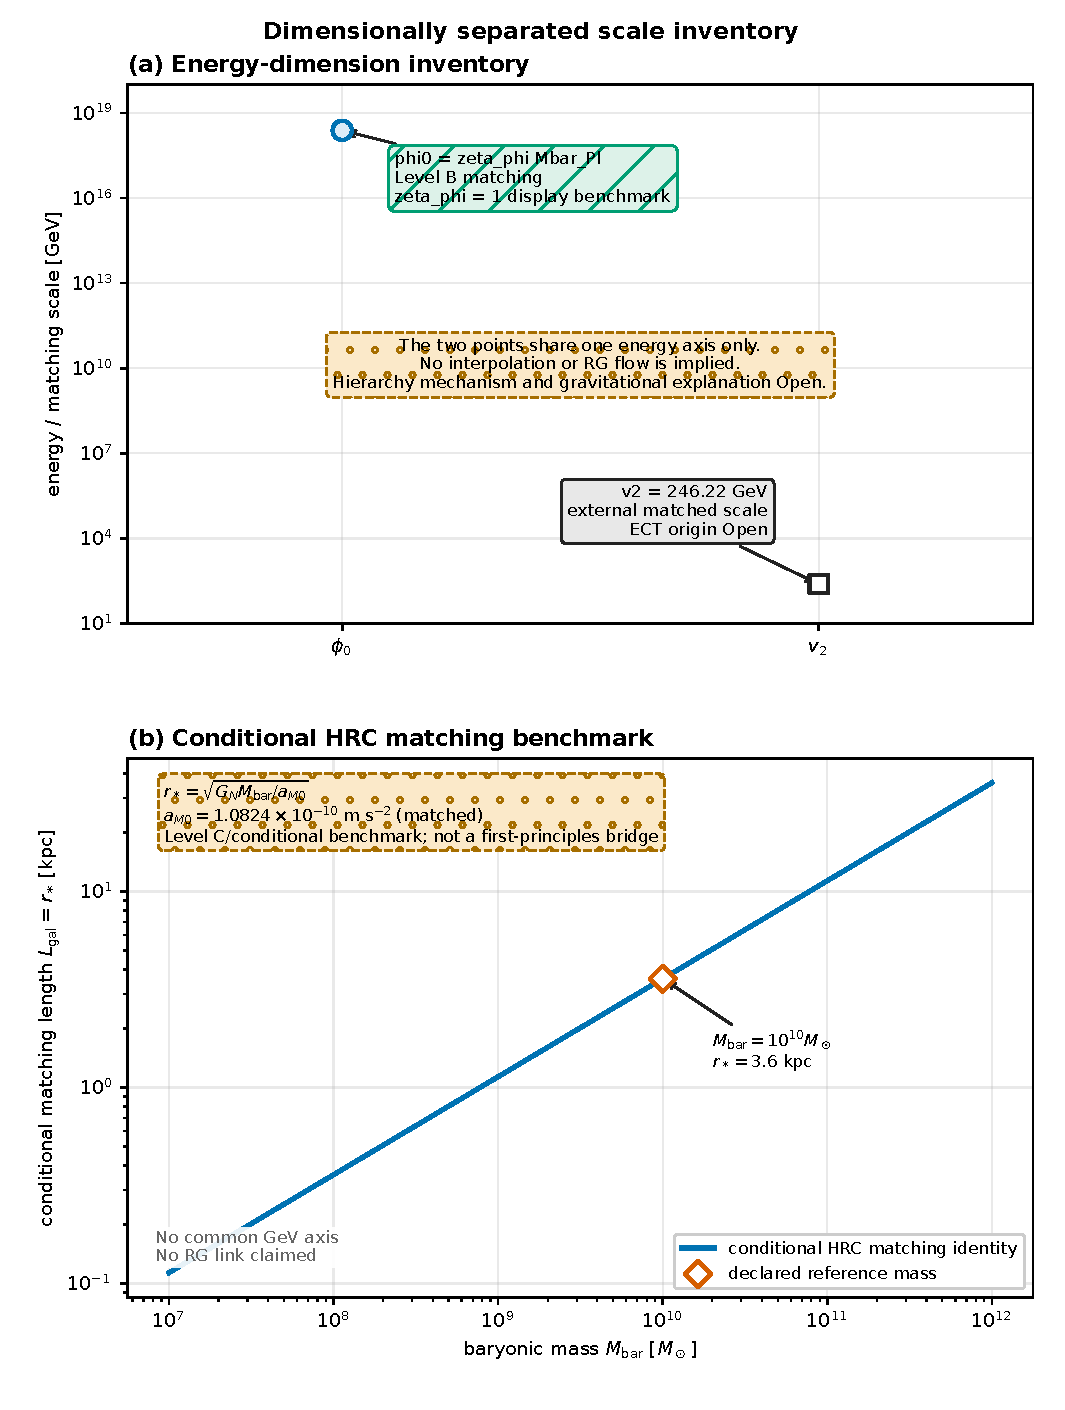
\includegraphics[width=\textwidth]{figures/r153/line_semantics/fig_condensate_scales_line_semantics_r153.pdf}
\caption{Dimensionally separated scale inventory.  Panel~(a) compares only
energy-dimension quantities; the origin of the matched electroweak scale and
the hierarchy mechanism remain Open.  Its two entries are independent
inventory points; no connecting curve or interpolation is implied.
Panel~(b) shows the conditional HRC
matching identity at the declared matched scale; it supplies no common GeV
axis or RG flow.  Colours encode structural, external, conditional and Open
roles and remain ordered by luminance in grayscale.}
\label{fig:three_condensate_scales}
\end{figure}
\FloatBarrier

\paragraph{Gravitational normalisation and the Planck scale.}
\label{par:planck_scale}
The parameter $u_0$ sets only the magnitude of the supplied P4
nonzero-gradient datum.  Neither an orientation stiffness nor dynamical
$O(4)\to O(3)$ breaking follows from it.
Moreover, $u_0$ cannot be identified directly with the reduced Planck mass:
the two quantities have different dimensions
($[u_0]=\text{GeV}^2$ in the present convention,
$[\bar{M}_{\rm Pl}]=\text{GeV}$).

In the supplied geometric-sector EFT, orientation variables $\delta n_i$
are assigned a kinetic term with effective stiffness
$\kappa_n = \mathcal{C}_n\,u_0^2$~(Section~\ref{sec:goldstone_soft_eft}),
where $\mathcal{C}_n$ is an effective coefficient with dimension
$\text{mass}^{-2}$.
A pure $P(X)$ closure of the ordered branch cannot generate this
term (Theorem~\ref{thm:PX_no_orientation}); orientation stiffness
therefore requires additional structure.  Candidate possibilities include
mixed radial--orientation dependence, an independent stiffness operator,
constraint-sector matching, higher derivatives, induced contributions, or
nonlocal response.  The two examples below are not exhaustive and no owner
is presently selected by P1--P6.
A generic orientation-sector heavy-field matching template may instead
be written
\begin{equation}
 \mathcal C_n
 =\frac{\hat a_n}{16\pi^2M_{n,\mathrm{heavy}}^2},
 \qquad
 \kappa_n=\mathcal C_nu_0^2 ,
 \label{eq:Cn_induced}
\end{equation}
where $M_{n,\mathrm{heavy}}$, the vertex that couples that field to
$(\partial n)^2$, the regulator, subtraction and finite coefficient
$\hat a_n$ must all be supplied by one stationary completion.  The current
P4 model owns none of them, so this is
\texttt{PARAMETRIC ONLY / MISSING VERTEX}; the P3 curvature
$m_{\Phi,\mathrm{rad}}$ cannot be inserted as $M_{n,\mathrm{heavy}}$ by
notation, and no equality to another sector's heavy scale is implied.
At equal mass dimension one may pose only the independent Open tensor bridge
\begin{equation}
 \boxed{M_G^2\stackrel{?}{=}c_M\kappa_n}
 \qquad\text{(Open representation and pole-residue map).}
 \label{eq:u0_Mpl}
\end{equation}

Separately from the Open tensor bridge, ECT adopts
\begin{equation}
  \boxed{\phi_0=\zeta_\phi\bar M_{\rm Pl}},
  \qquad \zeta_\phi>0,\ \zeta_\phi=O(1)
  \quad\text{(Level-B physical scale ansatz).}
  \label{eq:phi0_Mpl}
\end{equation}
The canonical benchmark $\zeta_\phi=1$ uses
$\bar M_{\rm Pl}=(8\pi G_N)^{-1/2}\approx2.435\times10^{18}$\,GeV.  A
first-principles derivation of $\zeta_\phi$, of $\mathcal C_n$, or of an
equation containing both $\phi_0$ and the tensor residue remains Open
(OP-Planck, Section~\ref{sec:open_problems}).

\paragraph{Planck-scale candidate: conditional dimensional route.}
The NLO estimate concerns orientation stiffness, not a graviton residue.
Only after a physical constrained tensor Hessian, matter vertex and
positive pole residue have been derived can $c_M$ be calculated and one ask
whether the adopted coefficient $\zeta_\phi$ is explained by the same owner.
At present $\phi_0=\zeta_\phi\bar M_{\rm Pl}$ is an explicit matching input,
not an induced-gravity result and not evidence that the Planck scale has been
derived from the condensate.

\paragraph{Common-medium hierarchy hypothesis.}
ECT adopts as a Level-B programme hypothesis that the P3/P4, electroweak,
infrared and HRC scales should admit a common-medium matching in a completed
theory.  No relation among $\phi_0$, $u_0$, $v_2$, $a_M$ and $m_\chi$ follows
at present unless it is displayed as a separate named closure.  The P3 length
$\xi_{\rm P3}=1/(\sqrt{2\lambda}\,\phi_0)$ and a future P4 pole length must
remain distinct; matching either to a Planck length requires an explicit
Planck convention and an independent dimensionless coefficient.

\paragraph{Connection to the universal structures already established.}
The hierarchy programme is not isolated from the rest of ECT.
The P3 amplitude $\phi_0$, a possible P4 orientation stiffness and
the coherent-sector action-scale programme
(\S\ref{par:action_scale_universality}) may share a future microscopic
completion, but no common matching owner is currently derived.  Whether it also owns a
physical tensor normalisation is precisely the Open bridge above; numerical
proximity to $\bar M_{\rm Pl}$ cannot establish that ownership.
A successful completion of the hierarchy problem must therefore be
compatible with all of those earlier universalities simultaneously.

\paragraph{The supplied gradient datum and the open problem OP-grad.}
Postulate~P4 introduces $u_0$ as the ordered-chart gradient scale
$\langle\partial_A\Phi\rangle = u_0\,\delta_{Aw}$, independently
of the bare potential minimum
$\phi_0 = \sqrt{\mu^2/\lambda}$~(P3).
P4 deliberately specifies the gradient datum independently of the
P3 field minimum.  Whether that datum belongs to a stationary physical
vacuum remains Open.  One may nevertheless write the following
Level-C dimensional ansatz by combining the homogeneous P3 amplitude
$\phi_0=\mu/\sqrt\lambda$ with its P3 Gaussian mass
$m_{\Phi,\mathrm{rad}}=\sqrt2\,\mu$; neither quantity is a P4 correlation
owner:

\begin{equation}
  u_0 \;\sim\; \frac{\phi_0}{\xi_{\rm P3}}
  \;\sim\; \phi_0\,m_{\Phi,\mathrm{rad}}
  \;\sim\; \frac{\mu}{\sqrt{\lambda}}\cdot\sqrt{2}\,\mu
  \;\sim\; \frac{\mu^2}{\sqrt{\lambda}}.
  \label{eq:u0_dimensional}
\end{equation}
This is only a dimensional self-consistency estimate, not a
derivation.
The action/state mechanism that could physically realise this gradient datum
remains an open foundational problem~(OP-grad).
Until OP-grad is closed, $u_0$ should be treated as an
independent Level~2 parameter~(Section~\ref{sec:param_hierarchy}).

\paragraph{Galactic HRC matching scale: conditional definition.}
The galactic sector introduces no second microscopic VEV.  Its present-epoch
matching value is $a_{M0}=cH_0/(2\pi)\approx1.08\times10^{-10}$\,m\,s$^{-2}$
for $H_0=70$\,km\,s$^{-1}$\,Mpc$^{-1}$.  This is a declared matching
condition, not a $\Phi$-medium postulate or a derived coefficient.  For a
declared $a_M$ and baryonic mass define
\begin{equation}
  r_* \equiv \left(\frac{G_N M_{\rm bar}}{a_M}\right)^{1/2};
  \label{eq:rstar_gal}
\end{equation}
for $M_{\rm bar}=10^{10}\,M_\odot$ and the matched value this is about
$3.6$\,kpc.  It is conditional HRC algebra: the internal response, gravity
bridge, source/metric map and microscopic owner of $a_M$ remain distinct
questions.
\begin{equation}
  \boxed{L_{\rm gal}\ \text{is a conditional HRC matching length; its ECT origin is Open.}}
\end{equation}

\paragraph{Why $a_M\sim cH_0$.}
In the present implementation,
$a_{M0}\equiv cH_0/(2\pi)\approx
1.08\times10^{-10}$\,m\,s$^{-2}$ is a declared Level-C matching
convention.  Its numerical proximity is therefore built into the
definition and is neither an ECT prediction nor evidence for a common
galactic--cosmological origin.  Such an origin would require one
microscopic action, source/force map, physical background solution and
observable matching calculation.  Those owners, and hence any derivation of
$a_M$ from condensate dynamics, remain Open
(OP-galactic; Section~\ref{sec:mp_galactic}).

\paragraph{Intermediate scale $v_2$ and the electroweak matching.}
If the ECT condensate undergoes a second ordering step, the
intermediate scale is fully fixed by low-energy matching:
\begin{equation}
  v_2 = \left(\sqrt{2}\,G_F\right)^{-1/2}
  \approx 246.22\,\text{GeV},
  \label{eq:v2_GF}
\end{equation}
where $G_F=1.1663785(6)\times10^{-5}$\,GeV$^{-2}$ is the
current PDG-2026 electroweak-review input~\cite{PDG2026EWWeb}.  The resulting
$v_2=246.21967\,$GeV is standard electroweak matching, not an ECT prediction.
This is not a free parameter: any deviation would give wrong
$W$ and $Z$ masses. A structural candidate mechanism for the
second transition $O(3)\to O(2)$ is discussed in
Appendix~\ref{app:second_transition}; it remains an open
problem of ECT.

\paragraph{Energy hierarchy and separate HRC matching length.}
Only the two energy-dimension quantities enter the hierarchy
\begin{equation}
  \phi_0 \sim \bar{M}_{\rm Pl} \gg v_2,
  \qquad
  \frac{v_2}{\phi_0} \approx 10^{-16}.
  \label{eq:hierarchy}
\end{equation}
Separately,
$L_{\rm gal}\equiv r_*=\sqrt{G_NM_{\rm bar}/a_M}$ is a
conditional HRC matching/crossover length; its fitted use is Level~C,
while the gravity bridge and origin of $a_M$ remain Open.  No dimensionally meaningful ordering
between $L_{\rm gal}$ and the energies above is implied.

\paragraph{The hierarchy problem in the ECT context.}
The ratio $v_2/\phi_0\approx 10^{-16}$ is the ECT counterpart of the
standard gauge hierarchy problem.
ECT does not solve this problem in the current formulation.
Under the adopted common-medium Level-B programme hypothesis, $v_2$ is
treated as the matching scale of a possible second ordering step within the
same condensate rather than as a fundamental VEV of an independent field
(Appendix~\ref{app:second_transition}).  The existence, action and dynamics of
that second step remain Open.  If it has a dynamical origin---for instance
through RG running of a supplied effective orientation coupling from
$\phi_0$ down to $v_2$ (Fig.~\ref{fig:three_condensate_scales})---the large
hierarchy could in principle be accommodated logarithmically rather than by
fine-tuning.
This is a structural possibility, not a derived result:
the explicit RG calculation within ECT has not been performed and
remains part of OP-EW.
Any claim that ECT resolves the hierarchy problem would be
premature.

\paragraph{Structural status of $v_2$ and its open-problem dependencies.}
\label{par:v2_status}
In the present formulation, $v_2$ is a matched intermediate scale, not
a first-principles condensate prediction. What remains open is not the
low-energy value $v_2=(\sqrt{2}G_F)^{-1/2}$ itself, but the dynamical
origin of the second ordering step within the same condensate.
A dimensional-analysis argument by itself cannot decide which mechanism,
if any, owns the hierarchy $v_2/\phi_0\sim10^{-16}$.
Polynomial or rational combinations of the primary ECT parameters
($\alpha$, $\beta$, $\lambda$, $\mu$, $u_0$, $\phi_0$) may merely relocate
the hierarchy into a small dimensionless coefficient unless a symmetry,
protection theorem or parameter measure is supplied; conversely, such
additional structure is a counterexample to any blanket polynomial no-go
claim.  The present work supplies no naturalness measure and proves no
uniqueness theorem.
Furthermore, any renormalisation-group-based derivation would require
$\beta$-functions of any supplied gauge completion, whose fields and
normalisations are not yet derived from condensate parameters. In that
sense, progress on OP-EW is structurally tied to the larger open programme
of constructing a local gauge sector (OP-SM).  The phase--orientation
alignment scenario of Appendix~\ref{app:second_transition} is one candidate
route, not an exhaustive or selected mechanism; its realisation remains
Open.

\paragraph{Exact reparameterisation and unresolved OP-EW-scale.}
\label{par:opew_scale_reduction}
The present parameter list does not select
$v_2/\phi_0\sim10^{-16}$.  Possible future mechanisms include protected
small parameters, dimensional transmutation, non-polynomial dynamics and
phase--orientation constructions; all remain Open.

We do not solve OP-EW here or reduce it uniquely to one mechanism.  The
observed hierarchy can be written, as an exact matched reparametrisation, as
\begin{equation}
  v_2 = \phi_0\, e^{-\mathcal{I}_{\rm EW}},
  \qquad
  \mathcal{I}_{\rm EW} \equiv \ln(\phi_0/v_2) \approx 36.8,
  \label{eq:I_EW_definition}
\end{equation}
where the numerical value follows from $\phi_0\simeq\bar M_{\rm Pl}=
2.435\times10^{18}$~GeV and $v_2=(\sqrt{2}G_F)^{-1/2}\approx
246.22$~GeV~\eqref{eq:v2_GF}, taken in their present matched form.

Equation~\eqref{eq:I_EW_definition} is only a logarithmic change of
variables.  It neither reduces the hierarchy problem nor identifies a
natural, preferred, or order-one microscopic input.  A physical derivation
would have to provide a protected secondary operator, its complete local
gauge and matter representations, the relevant beta functions or
nonperturbative dynamics, threshold matching, and a stability/radiative
closure.  None of these owners follows from P1--P7.  Accordingly no
particular scale-generation mechanism, including the candidate
phase--orientation constructions discussed later, is selected here.

\paragraph{Positioning relative to existing approaches.}
Dimensional transmutation as a route to the electroweak hierarchy
has a long history: classical scale invariance with radiative
breaking~\cite{Bardeen1995}, conformal extensions of the Standard
Model~\cite{MeissnerNicolai2007}, walking
technicolor~\cite{Holdom1981,Yamawaki1986}, and composite Higgs from
coset structures~\cite{AgasheContinoPomarol2005}. The novelty of the
ECT route, \emph{if} it can be closed, is that the running/critical
sector is not introduced as an external technicolor or conformal
sector but emerges from the phase--orientation structure of the
Euclidean condensate. The closest condensed-matter analogue is the
A$\leftrightarrow$B transition between ordered phases of superfluid
$^3$He~\cite{Volovik2003}, where two distinct broken-symmetry
patterns coexist within a single underlying condensate.

\paragraph{Discriminant with respect to the standard hierarchy problem.}
ECT reframes the hierarchy problem in a way that differs sharply from
the Standard Model.
In the Standard Model, the electroweak scale is the vacuum expectation
value of an independent Higgs field, while the Planck scale is an
external gravitational input.
In the current programme, $\phi_0$ and $m_\sigma$ belong to the real-scalar
model, while $S_0$, the TT gravitational scale and the electroweak scale
belong to separately supplied or matched closures.  A common microscopic
origin is a hypothesis to be tested, not a derived fact.
Thus the primary hierarchy question is no longer
``why are gravity and electroweak physics unrelated scales?''
but rather
``how does one condensate generate a secondary low-energy ordering step
$v_2\ll\phi_0$?''
This is still open, but it is a different and structurally narrower
problem.

The energy hierarchy and the separate HRC matching programme lead to three
distinct open problems:
\begin{description}
  \item[OP-grad (gradient condensate).]
    What is the dynamical mechanism by which the gradient
    condensate $\langle\partial_A\Phi\rangle = u_0\,\delta_{Aw}$
    emerges from the bare action P3?
    Dimensional analysis~\eqref{eq:u0_dimensional} is consistent,
    but a first-principles derivation remains open.
    A three-notion sharpening (local field equation;
    stationary-density magnitude selection; fluctuation-tensor
    matching) and the matching question M-($\alpha,\beta$) are
    recorded in the dynamic-motivation subsection; completion
    remains open.
  \item[OP-EW (electroweak hierarchy and locking programme).]
    Why does a second condensate scale arise at $v_2\ll\phi_0$, and how
    does the reduced orientation-sector transition extend to the full
    electroweak-like generator structure? The old single OP-EW problem
    is decomposed below into OP-EW-scale, OP-EW-locking, OP-EW-gauge,
    OP-EW-naturalness, and OP-EW-matter. The reduced
    $O(3)\to O(2)$ candidate is described in
    Appendix~\ref{app:second_transition}; the Hopf-fibered
    diagonal-locking upgrade is described in
    Appendix~\ref{app:hopf_locking}. Both remain structural
    programmes, not derived results.
  \item[OP-galactic (IR closure).]
    What determines $a_M$ and the corresponding $L_{\rm gal}$ from a
    microscopic ECT calculation?  The relation
    $a_M\sim cH_0/(2\pi)$ is a Level-C matched comparison/input.  Its coefficient,
    scalar-to-AQUAL source/force map, and condensate origin are Open.
\end{description}

\paragraph{Falsifier for the ECT hierarchy programme.}
The proposed common-origin hierarchy programme would fail if any of the
following were established:
(i)~the effective gravitational scale required a microscopic amplitude
parametrically unrelated to $\phi_0$;
(ii)~a named future completion predicted a P4 pole or validity scale
and that derived scale failed its prespecified matching test;
(iii)~the electroweak scale $v_2$ could only be introduced as the
vacuum expectation value of an entirely independent sector unrelated to
the original condensate;
or (iv)~the galactic scale and the cosmological background scale
required a second independent IR medium rather than branch variation of
the same condensate.
Conversely, an actual derivation tying $\phi_0$, $m_\sigma$, $S_0$, $M_G$
and secondary matching scales to one reduced action would support the
one-condensate hypothesis; no such derivation currently exists.

\paragraph{Programme-level hypotheses of the hierarchy architecture.}
The present ECT hierarchy picture lists four programme-level possibilities,
not current predictions or preferred expectations.
First, the P3 homogeneous radial curvature, a future action-owned
P4 pole/validity scale, the physical tensor normalisation and the Planck
energy are distinct owners.  A completed reduction may test a matching among
them; the current framework establishes no such correlation.
Second, any successful electroweak completion should generate $v_2$
as a secondary ordering or matching scale of the same medium, not as a
fundamental second vacuum unrelated to $\phi_0$.
Third, any future derivation of the HRC matching scale should connect it
to the same medium rather than introduce a third fundamental vacuum
expectation value; that connection is presently Open.
Fourth, a completed hierarchy solution inside ECT should reduce the
number of independent dimensionful inputs relative to the Standard
Model plus GR, not increase them.

\paragraph{Consistency programme for gravitational and quantum scales.}
ECT supplies a one-medium research architecture in which the scalar
characteristic speed is controlled by the ordered branch, while the
two reduced-loop action candidates and $G_N$ are conditional matching
programmes.  Mapping either $\Sigma_\theta\iota_0^{\rm EFT}$ or
$\Sigma_\theta\iota_{0,\rm bal}^{\rm eff}$ to the operational $S_0$, and then matching
$S_0\leftrightarrow\hbar$, requires a universality theorem, and $G_N$ exists here only through weak-field matching inside a
separately supplied gravity completion (Appendix~\ref{app:dim_audit}); the
condensate-to-tensor vertex and normalisation are Open.
At the current stage, however, their explicit parametrisations are not
yet fully reduced to an identical set of microscopic variables, because
the relation between the gradient condensate scale $u_0$ and the bare
potential data remains open~(OP-grad).
The relevant matching relations are:
\begin{equation}
  G_N^{\rm nat} = \frac{1}{8\pi M_G^2},
  \qquad
  \iota_0^{\rm EFT} = \frac{c_\perp\,K_\theta}{2\,m_\varphi^{2}},
  \label{eq:GN_S0_common}
\end{equation}
where $M_G$, $K_\theta$, and $m_\varphi$ belong to different
completion/matching layers.  Here the gravitational relation is in natural
units.  Only after the physical tensor residue and source vertex, clock/light
map and any scalar response are fixed may it be restored as
\begin{equation}
  G_N^{\rm SI}=\frac{\hbar c^5}{8\pi[E_{M_G}(\mathrm J)]^2},
  \qquad E_{M_G}[\mathrm J]\equiv
  M_G[\mathrm{GeV}](1\,\mathrm{GeV})_{\mathrm J}.
  \label{eq:GN_SI_energy_conversion}
\end{equation}
The $c$ in this SI conversion is the measured conversion speed; it is not an
unmatched use of $c_{\rm char}$.  The symbol $E_{M_G}$ is reserved for this
response-matching scale and must not be confused with the Diósi--Penrose
self-energy $E_G$ used in Sec.~\ref{sec:qs_decoherence}.  In the simplest supplied phase EFT one
estimates $K_\theta\sim\phi_0^2$ and
$m_\varphi=\sqrt{2\lambda}\,\phi_0$, where
$\phi_0=\sqrt{\mu^2/\lambda}$ is the bare field VEV;
Section~\ref{sec:hbar_status}).
Neither $G_N$ nor either loop coefficient is derived from the other.
The operational $S_0$, either candidate-owner map and its identification with
$\hbar$ remain parametric/Open, while $M_G$ needs
an independent nonzero TT completion before the first relation becomes
physical.  Their common microscopic origin is therefore an
architectural hypothesis to be tested, not an established consistency
relation.

\noindent\textbf{Status summary:}
\renewcommand{\arraystretch}{1.2}
\begin{longtable}{@{}L{7.1cm}L{2.5cm}L{4.9cm}@{}}
\toprule
Statement & Status & Comment \\
\midrule
\endfirsthead
\toprule
Statement & Status & Comment \\
\midrule
\endhead
\bottomrule
\endfoot
Supplied P4 gradient magnitude $u_0$
  & Input; UV/cutoff role Open
  & P4 owns no pole, correlation length or EFT breakdown scale \\
$P(X)\not\Rightarrow(\partial n)^2$ & A & Theorem~\ref{thm:PX_no_orientation} \\
$\kappa_n=\mathcal C_nu_0^2$; $M_G^2\stackrel{?}{=}c_M\kappa_n$ & A for orientation coefficient / Open tensor bridge & Equal dimensions do not derive a tensor owner \\\
$M_G=\bar{M}_{\rm Pl}$ (weak-field matching) & B & Section~\ref{sec:GN_matching} \\
$\phi_0=\zeta_\phi\bar{M}_{\rm Pl}$, $\zeta_\phi>0,\ \zeta_\phi=O(1)$
  & Adopted Level~B scale ansatz / microscopic explanation Open
  & Independent of the still-Open tensor bridge \\
$u_0\sim\phi_0\cdot m_\varphi$: dimensional
  self-consistency & B & Eq.~\eqref{eq:u0_dimensional};
  OP-grad \\
$v_2=(\sqrt{2}G_F)^{-1/2}$ as IR matching constraint & Constraint & If second transition exists \\
Galactic HRC response and scale & A/B/C/Open by layer & Response and BTFR slope algebra are A inside supplied models; BTFR is B after the declared bridge; bridge and $a_M$ ownership Open; data comparison C \\
$a_M\sim cH_0/(2\pi)$: matched comparison/input & C / origin Open &
  Coefficient and microscopic map Open (OP-galactic) \\
$G_N$ and the two loop candidates share a proposed one-medium matching programme
  & Open ownership & Eq.~\eqref{eq:GN_S0_common} displays only the fixed-core
  branch; the balanced branch additionally requires $\mathcal T_{\rm loop}$.
  No common owner, universality map or physical tensor vertex is derived \\
$\mathfrak{so}(3)\cong\mathfrak{su}(2)$: structural compatibility
  with EW-like second transition & A & Algebra only \\
Reduced $O(3)\to O(2)$ transition as orientation-sector analogue
  & B/C & Two broken directions only; not full EW counting \\
Gradient condensate from bare action & Open (OP-grad) & \\
Hopf-fibered diagonal locking
$\mathrm{SU}(2)_{\rm orient}\times\mathrm{U}(1)_\theta\to
\mathrm{U}(1)_{\rm diag}$
  & Candidate geometry & Three broken directions at pre-gauge/global level;
  dynamics not derived (App.~\ref{app:hopf_locking}) \\
Origin of compact $\mathrm{U}(1)_\theta$ as EW-locking participant
  & Open (OP-EW-locking.0) & Effective phase sector exists; EW role not derived \\
First-principles derivation of $v_2$
  & Open (OP-EW-scale) & The logarithmic identity
    $\mathcal I_{\rm EW}=\ln(\phi_0/v_2)$ supplies no generating dynamics \\
Local chiral gauge completion, hypercharge, $g$, $g'$, Weinberg angle
  & Open (OP-EW-gauge) & Not implied by Hopf geometry alone \\
Radiative protection of $\sigma_2$
  & Open (OP-EW-naturalness) & Goldstone protection does not protect radial mode \\
First-principles derivation of $a_M$ & Open (OP-galactic) & \\
\bottomrule
\end{longtable}

\subsection{Parameter hierarchy by level of description}
\label{sec:param_hierarchy}

\paragraph{Level 1. Bare micro-parameters~(P3).}
The potential $V(\Phi)$ contains two parameters:
$\mu^2>0$, $\lambda>0$, with bare radial stiffness:
\begin{equation}
  m_\sigma^2 = V''(\phi_0) = 2\mu^2,\qquad
  \phi_0 = \sqrt{\mu^2/\lambda}.
  \label{eq:sigma_mass}
\end{equation}
These characterise the microscopic field dynamics only and
do not derive the P4 gradient datum or a physical ordered vacuum.

\paragraph{Level 2. Supplied ordered-chart parameters~(P4).}
Postulate~P4 introduces $u_0>0$, the gradient scale
$\langle\partial_A\Phi\rangle = u_0\,\delta_{Aw}$.
This is an independent parameter; its relation to $\phi_0$
and $\lambda$ from the bare theory requires additional
matching (OP-grad).

\paragraph{Level 3. Conditional ordered-chart EFT parameters.}
The effective kinetic tensor contains $\alpha>\beta>0$ and $m_{\rm eff}^2$,
where $m_{\rm eff}^2\neq m_\sigma^2$ in general.

\paragraph{Level 4. Coherent-sector parameters~(BR1).}
Within a supplied compact-phase EFT~(BR1), winding supplies only the integer
label.  A fixed-core route defines $\iota_0^{\rm EFT}$ by evaluating the
phase-gradient functional at a supplied $L_{\rm core}$; an alternative
positive-tension route defines $\iota_{0,\rm bal}^{\rm eff}$ by a conditional
minimum (Section~\ref{sec:hbar_status}).  The 4D owners, route selection,
cross-sector universality and map to operational $S_0$ remain Open.
The separate calibration $S_0\leftrightarrow\hbar$ is retained as a
Level~B physical matching, not as a microscopic derivation.

\subsection{Dimensionless scalar slope and physical-speed map}
\label{sec:c_star}

\textit{Status: Level~A mathematics for $\hat c_*$ in the supplied
scalar EFT; $\hat c_*=1$ is a Level-B unit-slope coefficient benchmark;
$c_{\rm char}=c$ is an adopted Level-B scalar-clock calibration; photon and
tensor cone matching remains Open.}

From the dispersion relation~\eqref{eq:dispersion}:
\begin{equation}
  \label{eq:c_star_def}
  \boxed{\hat c_*^2=\frac{\beta}{\alpha-\beta}.}
\end{equation}
This is a strict EFT consequence; it requires neither quantum
formalism nor a gravitational sector.

\paragraph{Physical clock and observational matching.}
Equation~\eqref{eq:c_star_def} fixes only the common-length slope.
After an independent conversion speed $c_{\rm u}$ and clock lapse
$\mathcal N_\Phi$ are supplied,
$c_{\rm char}=c_{\rm u}\hat c_*/\mathcal N_\Phi$.
The equality $c_{\rm char}=c$ is adopted as the scalar-clock
calibration.  The further equality $c_\gamma=c_{\rm char}$ requires the
missing photon owner, while GW170817 constrains an independently missing
tensor principal symbol~\cite{LIGO_Fermi_GW170817_GRB2017}.
The benchmark coefficient choice $(\beta,\alpha)=(1,2)$ combines the
Level-B unit-slope benchmark $\hat c_*=1$ with the convention $\beta=1$;
a common field rescaling cannot select the
ratio $\alpha/\beta$.
The parameters $(\alpha,\beta)$ are EFT parameters not derivable
from the bare micro-action P3 in the current formulation.


% R103:T2 scale owner
\subsection{Conditional tensor scale and Newton's constant}
\label{sec:GN_matching}

The orientation coefficient $\kappa_n=\mathcal C_nu_0^2$ has mass dimension
two.  The fixed-map theorem shows that it does not normalise a helicity-2
field in the currently displayed director channel.  Introduce instead $M_T$
as the coefficient of a \emph{separately supplied} healthy tensor action.  In
that conditional EFT the standard weak-field matching is
\begin{equation}
G_N^{\rm nat}=\frac{1}{8\pi M_T^2}.
\end{equation}
This relation defines the matched $M_T$ once the physical metric and vertex
are specified.  A microscopic bridge $\kappa_n\to M_T^2$ is Open; neither
dimensional analysis nor an induced orientation term supplies it.

\subsection{Radial-mode scales and the correlation length}
\label{sec:sigma_scales}

The homogeneous P3 potential owns the local curvature
\begin{equation}
  m_{\Phi,\mathrm{rad}}^2:=V''(\phi_0)=2\mu^2 .
\end{equation}
For that homogeneous P3 fluctuation, the Euclidean propagator has the
large-distance behaviour
$G_{\Phi,\mathrm{rad}}(r)\propto
e^{-m_{\Phi,\mathrm{rad}}r}/r^{3/2}$, so its correlation length is
$\xi_{\rm P3}=m_{\Phi,\mathrm{rad}}^{-1}$ within P3
(Appendix~\ref{app:corr_length}).  This result does not own a fluctuation
about the independently postulated P4 gradient background.

A P4 pole and correlation length require a stationary P4 action, boundary
and constraint data, and the constrained Hessian
\begin{equation}
  \mathcal H_{\rm P4}
  =\left.\frac{\delta^2S_{\rm P4}}
  {\delta\Phi\,\delta\Phi}\right|_{\bar\Phi_{\rm P4}},
  \qquad
  \xi_{\rm P4}^{-1}:=m_{\rm P4,pole}.
  \label{eq:p4_hessian_owner}
\end{equation}
None is presently supplied.  Thus
$m_{\rm P4,pole}=m_{\Phi,\mathrm{rad}}$ and
$\xi_{\rm P4}=\xi_{\rm P3}$ are Open matching hypotheses, not identities.

The exact P3 relation
$m_{\Phi,\mathrm{rad}}=\sqrt{2\lambda}\,\phi_0$ does not fix a Planck-scale
mass or Planck-length correlation scale because $\lambda$ is an independent
owner.  It neither establishes a Planck-heavy P4 particle nor follows from
the reduced phase-loop coefficient.  The latter is
dimensionless; its physical match is
$\Sigma_\theta\,\iota_0^{\rm EFT}=\hbar$ with independent, Open
$\Sigma_\theta$.  Consequently Eq.~\eqref{eq:S0_lambda} alone fixes neither
$\lambda$ nor either radial pole.  The separate P3, P4 and secondary
electroweak radial statuses are developed in
Section~\ref{sec:radial_mode}.

\subsection{Dimensionless loop coefficients and the Open physical action normalisation}
\label{sec:hbar_status}

\textit{Status: three-layered with two explicitly distinct Layer-2
closures.  Layer~1 is Level-A variational mathematics for a dimensionless
reduced functional in a supplied $U(1)$-extended phase model.  Layer~2a
defines the dimensionless fixed-core coefficient $\iota_0^{\rm EFT}$ after a
loop length is supplied.  Layer~2b defines the distinct dimensionless
balanced coefficient $\iota_{0,\rm bal}^{\rm eff}$ after a positive line
tension is supplied.  At $n=1$ and $L_{\rm core}=L_{*,1}$ they differ by a
factor of two and must not be conflated.  The compact phase, carrier,
profile, tension and common four-dimensional owner remain Level-B/Open.
Layer~3 introduces a separate action-valued normalisation $\Sigma_\theta$;
only products such as $\Sigma_\theta\iota_0$ may be matched to the
operational $S_0$ and then to $\hbar$.  This is calibration, not a
parameter-free derivation.}

A central question for ECT is whether the physical universal quantum of
action can be derived from the coherent branch rather than supplied.
The present framework does not settle that question.  It instead
exhibits two dimensionless reduced-model coefficients: the phase-only
fixed-core $\iota_0^{\rm EFT}$ and the tension-balanced
$\iota_{0,\rm bal}^{\rm eff}$.  Neither is an action.  A physical Euclidean phase-loop action requires
$S_{\theta,E}^{\rm phys}=\Sigma_\theta\mathcal I_{\theta,E}$ with a finite
positive owner-specific action-dimension constant $\Sigma_\theta>0$.
Positivity preserves the reduced stationary points and minima; it does not by
itself define a statistical suppression factor.  If a positive Euclidean
loop measure is later supplied, it needs an independent denominator
$\Sigma_{\rm PI,\theta}>0$ and the dimensionless exponent
$\kappa_\theta\mathcal I_{\theta,E}$, where
$\kappa_\theta=\Sigma_\theta/\Sigma_{\rm PI,\theta}$.  Neither this
denominator nor its equality to $S_0$ is derived.  Reusing
$\Sigma_\theta$ in the Lorentzian phase action is a separate same-sector
continuation/matching input, not a consequence of winding.  Only then can
$\Sigma_\theta\iota_0$ be compared with the operational $S_0$ and the
observed $\hbar$.  What follows separates the exact reduced mathematics from these
Open owner and matching maps.
Appendix~\ref{app:action_scale_S0} collects the periodicity, fixed-core, and
action-normalisation chain with the same status separation.

Phase single-valuedness fixes integer winding at fixed loop data, but it
does not supply the compact phase sector, transverse profile, core length,
line tension, operational action unit or universal quantum of action.

% ============ LAYER 1 ============

\paragraph{Layer~1: compact phase and the variational bound
(strict within the reduced $U(1)$-extended phase-loop EFT).}

\emph{Coherent phase variable.}
In the smooth coherent branch~(BR1), the collective state is
characterised not only by an amplitude $\rho$ but also by a
phase-like variable~$\theta$.
Because the coherent state is physically single-valued, this phase
is defined only modulo a full winding:
\begin{equation}
  \theta \sim \theta + 2\pi.
  \label{eq:theta_periodicity}
\end{equation}
It should be noted that the real scalar field $\Phi$ of P3 does not
by itself carry a compact $U(1)$ phase variable.
The extension to $\Phi_{\rm eff}=\rho\,e^{i\theta}$ is an additional
modelling step for the coherent charged sector.
Accordingly, the periodicity $\theta\sim\theta+2\pi$ and the
associated winding number are strict statements within the
$U(1)$-extended phase EFT, not direct topological consequences of the supplied director orbit
$O(4)/O(3)\simeq S^3$ (which has $\pi_1(S^3)=0$).

\emph{Dimensionless reduced phase functional.}
Conditional on a supplied phase sector and amplitude freeze-out, write
\begin{equation}
  \mathcal I_{\theta,E}[\theta]
  = \frac{K_\theta}{2}
    \int d^4X\;\delta^{AB}\partial_A\theta\partial_B\theta,
  \qquad
  S_{\theta,E}^{\rm phys}:=\Sigma_\theta\mathcal I_{\theta,E},
  \label{eq:S_theta_layer1}
\end{equation}
where $\mathcal I_{\theta,E}$ is the positive Euclidean reduced loop
functional, dimensionless in the printed natural-unit normalisation, and
$\Sigma_\theta$ is an independent action-valued coefficient.  The retained
Gaussian phase closure assumes the same supplied stiffness
$K_\theta=K_\theta^{\rm eff}>0$; zero is degenerate, while a negative value
does not define the positive Euclidean functional used in this layer.
In the simplest quartic bare-potential realisation one expects
$K_\theta\sim\phi_0^2$, where $\phi_0=\sqrt{\mu^2/\lambda}$.  Throughout this section and
Appendix~\ref{app:Sloop_calc}, $K_\theta$ is an abbreviation for the same
supplied coherent-branch stiffness denoted $K_\theta^{\rm eff}$ in
Part~III; it is not an independently adjustable bare coefficient.  The owner
map used below is therefore
$K_\theta^{1\mathrm D}=K_\theta^{\rm eff}\mathcal A_\perp$.  If a microscopic
reduction produces a different coefficient, the fixed-core and balanced-loop
constructions must be treated as a different model rather than silently
identified with the Part~III branch.

\emph{One-dimensional reduction and the transverse three-volume
weight.}
For a supplied closed one-dimensional Euclidean carrier the
four-dimensional phase action reduces to an effective one-dimensional
functional only after integrating its localised profile over the three
transverse coordinates.  This geometry is a codimension-three curve or
worldline; it is not, by this notation alone, a spatial vortex tube.
We encode this reduction in the effective one-dimensional stiffness
\begin{equation}
  K_\theta^{1\mathrm D}
  \;\equiv\;
  K_\theta\,\mathcal A_\perp ,
  \qquad
  \mathcal A_\perp = c_\perp\,\xi_{\rm core}^{3},
  \qquad
  [K_\theta^{1\mathrm D}]=\text{GeV}^{-1},
  \label{eq:Ktheta_1D}
\end{equation}
where $\xi_{\rm core}\sim m_\varphi^{-1}$ is the radial-core scale and
$c_\perp=\mathcal O(1)$ is a profile-dependent geometric coefficient of
the transverse three-volume weight that is \emph{not} fixed at the
present EFT level (Appendix~\ref{app:Sloop_calc}).
This step is a dimensionally consistent reduced-loop closure, not a
first-principles derivation of the transverse profile~(Level~B).

\emph{Sharp lower bound on the dimensionless carrier functional
(Cauchy--Schwarz inequality).}
Consider a supplied closed one-dimensional carrier $\gamma$ of proper
length $L$
in the phase EFT with winding number
$n[\gamma]=\frac{1}{2\pi}\oint_\gamma\partial_\ell\theta\,d\ell$.
The dimensionless reduced 1D functional along the loop, built on the
reduced one-dimensional stiffness~\eqref{eq:Ktheta_1D}, is
\begin{equation}
  \mathcal I_{\rm loop}[\theta]
  = \frac{K_\theta^{1\mathrm D}}{2}\oint_\gamma d\ell\;
    (\partial_\ell\theta)^2.
  \label{eq:S_loop_def}
\end{equation}
By the Cauchy--Schwarz inequality applied to the constant function
$f=1$ and $g=\partial_\ell\theta$:
\begin{equation}
  \oint d\ell\;(\partial_\ell\theta)^2
  \;\geq\;
  \frac{1}{L}\left(\oint d\ell\;\partial_\ell\theta\right)^{\!2}
  = \frac{(2\pi n)^2}{L},
  \label{eq:CS_inequality}
\end{equation}
with equality if and only if $\partial_\ell\theta=\text{const}$
along the loop (uniform winding).
Therefore:
\begin{equation}
  \boxed{\mathcal I_{\rm loop}[\theta]
  \;\geq\;
  \frac{2\pi^2 K_\theta^{1\mathrm D}\,n^2}{L},
  \qquad
  \text{equality at uniform winding.}}
  \label{eq:loop_bound}
\end{equation}
This is a strict variational result inside the supplied reduced model:
the minimiser of the dimensionless loop functional at fixed length and
winding is the uniform-gradient configuration, and its minimum scales as
$n^2/L$.

\emph{Important structural remark.}
Equation~\eqref{eq:loop_bound} provides a sharp lower bound for
each fixed $L$, but because the bound falls as $1/L$,
$\mathcal I_{\rm loop}\to 0$ as $L\to\infty$.
The pure phase topology alone does \emph{not} yield a nonzero
global minimum of the reduced functional; additional physical input is
needed even to define a distinguished dimensionless coefficient, and
$\Sigma_\theta$ is still required to obtain an action.

% ============ LAYER 2 ============

\paragraph{Layer~2: supplied loop scales and dimensionless
coefficients (Level~A mathematics / Level~B--Open ownership).}

\emph{Why the fixed-$L$ bound is not yet a nonzero global minimum.}
Equation~\eqref{eq:loop_bound} gives the minimum of the
dimensionless reduced functional in a fixed length-and-winding sector, but
because the bound falls as $1/L$, it does not define a nonzero global reduced
minimum when the loop length is allowed to vary.  A physical action requires
the independent positive factor $\Sigma_\theta$.

\emph{Supplied carrier-length benchmark.}
To obtain a distinguished fixed-core dimensionless EFT coefficient, one
must supply the proper length or period of an elementary closed carrier.  A core-sized
benchmark
may be written
\begin{equation}
  L_{\rm core}\sim 2\pi\,\xi_{\rm core}
  = \frac{2\pi}{m_\varphi}.
  \label{eq:Lcore}
\end{equation}
This is a Level~B/Open convention, not a consequence of topology or of the
straight-vortex profile.  The local correlation length motivates a
transverse scale but does not select a spatial circumference, Euclidean
proper period or worldline ensemble.  In particular, a localised-carrier
expansion does not fail merely because $L\gg\xi_{\rm core}$; curvature and
profile corrections instead become important when the radius of curvature
approaches the core width.  A physical interpretation of $L$ therefore
requires a separate embedding, ensemble and stabilisation mechanism.

\emph{Core-width calculation and carrier guard.}
The estimate $\xi_{\rm core}\sim m_\varphi^{-1}$ follows in a supplied
straight global-vortex problem for the $(\rho,\theta)$ system.  This is a
codimension-two profile analogy; without an explicit embedding and
dimensional reduction it does not own the codimension-three $d^3y$
worldline coefficient used above.
For a rectilinear vortex with unit winding, the radial profile
$\rho(r)$ satisfies $\rho(0)=0$ and $\rho(r)\to\phi_0$ at
$r\gg m_\varphi^{-1}$, with the core size fixed by the balance
between gradient energy and potential energy at
$\xi_{\rm core}\sim m_\varphi^{-1}$.
For a closed loop of circumference $L\sim 2\pi\xi_{\rm core}$,
curvature corrections are $O(1)$ and do not change the scaling
estimate.
It does not identify the circumference of an elementary closed loop or a
nonzero global action minimum.  The order statement
$L_{\rm core}=O(\xi_{\rm core})$, with
$L_{\rm core}=2\pi\xi_{\rm core}$ as the explicit benchmark used above,
remains a Level-B/Open closure choice pending the full 4D closed-loop
variational problem.

\emph{Defined fixed-core dimensionless coefficient.}
Evaluating the fixed-$L$ lower bound~\eqref{eq:loop_bound} at the
supplied elementary-loop size with $n=1$ gives
\begin{equation}
  \iota_{\rm elem}
  := \frac{2\pi^2 K_\theta^{1\mathrm D}}{L_{\rm core}}
  = \pi\,c_\perp\,\frac{K_\theta}{m_\varphi^{2}},
  \qquad
  S_{\rm elem}^{\rm phys}:=\Sigma_\theta\iota_{\rm elem}.
  \label{eq:S_elem}
\end{equation}
Define
\begin{equation}
  \boxed{\iota_0^{\rm EFT}
  \;\equiv\;
  \frac{\iota_{\rm elem}}{2\pi}
  = \frac{c_\perp\,K_\theta}{2\,m_\varphi^{2}}.}
  \label{eq:S0_EFT}
\end{equation}

\emph{Dimensionless form and parameter compression.}
In the simplest quartic realisation
(in the convention $V(\Phi)=-\tfrac{\mu^2}{2}\Phi^2
+\tfrac{\lambda}{4}\Phi^4$ of~P3, so that $K_\theta\sim\phi_0^2$ and
$m_\varphi^2=2\lambda\,\phi_0^2$)
the elementary-loop scale becomes
\begin{equation}
  \iota_0^{\rm EFT}\;\sim\;\frac{c_\perp}{4\lambda},
  \label{eq:S0_lambda}
\end{equation}
independent of $\phi_0$ inside this supplied profile and normalisation.
It is not an ECT prediction because $K_\theta$, $c_\perp$, the loop length
and the real-to-complex reduction are not derived.
Consequently the conditional physical matching
$\Sigma_\theta\,\iota_0^{\rm EFT}=\hbar$ constrains only the product
$\Sigma_\theta c_\perp/(4\lambda)$.  Because $\Sigma_\theta$ and
$c_\perp$ are not independently derived, it neither fixes $\lambda$ nor
constitutes a parameter-free prediction.
This is a candidate dimensionless EFT coefficient after the fixed-core
closure is supplied, not a topologically selected or globally minimal
physical action scale.  Only
$\Sigma_\theta\iota_0^{\rm EFT}$ is action-valued
(Level~A reduced algebra / Level~B route / Open owner).

\emph{Notation.}
The dimensionless fixed-core representative is
$\iota_{\rm elem}^{\rm(fixed\ core)}=2\pi\iota_0^{\rm EFT}$, while its
physical action would be
$S_{\rm elem}^{\rm phys}=\Sigma_\theta\iota_{\rm elem}^{\rm(fixed\ core)}$.
The supplied length and coefficient are not fixed by topology, and no global
variational minimum over arbitrary loop lengths is asserted.

\emph{Optional tension-balanced closure route (additional supplied physics).}
A different, constructive way to remove the $L\to\infty$ zero-infimum is to
supply the same reduced one-dimensional carrier with a positive reduced
inverse-length coefficient $\mathcal T_{\rm loop}$.  For
$K_\theta^{1\mathrm D}>0$,
$\mathcal T_{\rm loop}>0$ and nonzero winding $n$, the supplied dimensionless
1D model is
\begin{equation}
  \mathcal I_n(L)=\mathcal T_{\rm loop}L
  +\frac{2\pi^2K_\theta^{1\mathrm D}n^2}{L},
  \qquad L>0,
  \qquad
  [K_\theta^{1\mathrm D}]=L,\quad
  [\mathcal T_{\rm loop}]=L^{-1}.
  \label{eq:tension_balanced_loop_functional}
\end{equation}
In the phase route the physical coefficients are
$K_{\theta,\rm phys}^{1\mathrm D}
=\Sigma_\theta K_\theta^{1\mathrm D}$ and
$\mathcal T_{\theta,\rm phys}
=\Sigma_\theta\mathcal T_{\rm loop}$, with dimensions action times length
and action per length, respectively.  The reduced coefficients do not supply
the action unit.
It is strictly convex for every $L>0$ and diverges at both ends of
the allowed interval.  Hence, at fixed nonzero winding and within this
one-coordinate ansatz, it has a unique global minimum with respect to $L$:
\begin{equation}
  L_{*,n}=\pi |n|\sqrt{\frac{2K_\theta^{1\mathrm D}}
                                  {\mathcal T_{\rm loop}}},
  \qquad
  \mathcal I_{n,\min}=2\pi |n|\sqrt{2K_\theta^{1\mathrm D}
                                  \mathcal T_{\rm loop}},
  \label{eq:tension_balanced_minimum}
\end{equation}
with equal tension and phase-gradient contributions at $L_{*,n}$.  For
$n=0$, however, $\mathcal I_{n=0}(L)=\mathcal T_{\rm loop}L$ has infimum zero as
$L\to0^+$ and no finite interior minimum.  It is useful to define the
balanced-model scale
\begin{equation}
  \iota_{0,\rm bal}^{\rm eff}
  \equiv \frac{\mathcal I_{1,\min}}{2\pi}
  =\sqrt{2K_\theta^{1\mathrm D}\mathcal T_{\rm loop}}.
  \label{eq:S0_bal_eff}
\end{equation}
This symbol is deliberately distinct from the phase-only fixed-core
$\iota_0^{\rm EFT}$.  For the elementary sector $n=1$, if one chooses
$L_{\rm core}=L_{*,1}$ and evaluates only the phase-gradient term used in
the fixed-core definition, then
\begin{equation}
  \left.\iota_0^{\rm EFT}\right|_{L_{\rm core}=L_{*,1}}
  =\frac12 \iota_{0,\rm bal}^{\rm eff}.
  \label{eq:S0_bal_fixed_relation}
\end{equation}
Thus, at the same elementary $n=1$ length, the balanced total coefficient is
twice the phase-only coefficient.  This factor is a normalisation consequence
of the two equal contributions and is not, by itself, evidence of double
counting.

The minimisation in Eqs.~\eqref{eq:tension_balanced_loop_functional}--
\eqref{eq:S0_bal_fixed_relation} is Level~A mathematics inside the supplied
1D model.  Its ECT interpretation is only a Level~B/Open route: the compact
$U(1)$ sector, transverse profile, positive length-independent tension,
the correct worldline or worldsheet embedding, declared ensemble, shape
modes, curvature, collapse, splitting and self-intersection terms,
unwinding barriers and backreaction
must be obtained from one 4D reduced action.  In particular,
$\mathcal T_{\rm loop}$ and $K_\theta^{1\mathrm D}$ cannot be fitted as
unrelated knobs, and no equation above derives $\hbar$ from P1--P6.  The
full ownership and falsification conditions are collected in
Appendix~\ref{app:Sloop_calc}.

\emph{Post-order candidate constitutive hypothesis CDE-$\Phi$: cohesive
defect elasticity.}
CDE-$\Phi$ is not a pre-physical property, a new frozen postulate or an
action owner.  It is a branch-EFT acceptance criterion: after an ordered
branch and its dynamics have already been declared, at least one stationary
localised profile must heal to the ambient state, have a positive reduced
line coefficient together with a finite positive physical-action prefactor,
and have a positive projected metric on each retained physical normalisable
modulus.  In plain
language, a completed branch must be able to hold a localised disturbance
together, and both extending it and varying a genuine internal coordinate
must cost positive action.  This criterion mentions neither gravity nor
quantisation and supplies no compact modulus, topology, rigidity, measure or
action quantum.

The actual owner is the full tuple consisting of an explicit
four-dimensional completion action, its physical state and boundary data, a
stationary profile, one fixed vacuum subtraction and regulator, and the
constraint/gauge/frame/zero-mode quotient used to define physical
fluctuations.  Suppose that tuple supplies completion fields
$\Psi^I$ (which may include an independent orientation or other collective
field and are not silently identified with the single real P3 scalar
$\Phi$), a stationary localised profile
$\Psi_*^I(y;\vartheta)$ around a one-dimensional Euclidean carrier
$X^A(s)$, and a genuine compact normalisable collective coordinate
$\vartheta\sim\vartheta+2\pi$ after the physical quotient.  A controlled
collective-coordinate reduction~\cite{Manton1982Moduli} can then have the
dimensionless reduced form
\begin{equation}
 \begin{aligned}
 \mathcal I_{E,\rm red}^{\rm sub}
 &=\int ds\left[
   \mathcal T_{\rm loop}
   +\frac{K_\vartheta^{1\mathrm D}}{2}
      \left(D_s\vartheta\right)^2
   +\frac{\kappa_b}{2}\,\mathcal K^2
   +\cdots\right],\\
 S_{E,\rm phys}^{\rm sub}
 &=\Sigma_\vartheta\mathcal I_{E,\rm red}^{\rm sub},
 \qquad \Sigma_\vartheta>0 .
 \end{aligned}
 \label{eq:cde_phi_worldline_reduction}
\end{equation}
where $\mathcal K$ is the carrier curvature, $D_s$ contains any derived
normal-bundle or internal connection, and the ellipsis is deliberately
non-exhaustive: twist, torsion, mixed curvature--modulus, nonlocal and
higher-derivative terms must be retained whenever the owner permits them.
Before profile relaxation, the two leading coefficients are schematically
\begin{align}
 \mathcal T_{\rm loop}
 &=\int d^3y\,
   \bigl[\mathcal L_E(\Psi_*;\mathfrak s)
         -\mathcal L_E(\Psi_{\rm vac};\mathfrak s)\bigr],
 \label{eq:cde_phi_tension_owner}\\
 K_\vartheta^{1\mathrm D}
 &=\int d^3y\,
   G_{IJ}(\Psi_*;\mathfrak s)\,
   \partial_\vartheta\Psi_*^I\,
   \partial_\vartheta\Psi_*^J ,
 \label{eq:cde_phi_moduli_metric}
\end{align}
where $\mathfrak s$ records the state and boundary data.
The physical coefficient is obtained only after constrained profile
relaxation, gauge reduction and the corresponding Schur complement.
Equations~\eqref{eq:cde_phi_tension_owner} and
\eqref{eq:cde_phi_moduli_metric} show how the two parameters could be
computed from one action rather than postulated independently.  They are a
derivation template, not evidence that the minimal real-scalar P3 action has
the required profile or compact modulus.

The transverse $d^3y$ measure is crucial.  It describes a codimension-three
curve in four-dimensional Euclidean space---most naturally the worldline of
a point-like texture on a selected three-dimensional slice.  A spatial
$U(1)$ vortex loop persisting along the selected $w$ direction instead
traces a two-dimensional worldsheet, has a transverse $d^2y$ reduction, and
would make the bracketed expression an energy or an action per unit
$w$-duration.  These two embeddings are not interchangeable.
Here $L=\int_\Gamma ds$ is the proper length or Euclidean period of the
closed worldline, not the spatial radius of the texture.  Varying $L$ is
meaningful only in a declared closed-worldline/proper-time ensemble with its
einbein or parametrisation convention, boundary period and measure fixed.
For propagation over a prescribed duration, or when $L$ is a gauge modulus,
$L$ is external and the stationary-length calculation is not a physical
size prediction.
Current-carrying string constructions provide an external example in which
the string carrier and a longitudinal internal mode are separate
ingredients~\cite{Witten1985Superconducting}; they do not derive either
ingredient in ECT.

The best-matched ECT-native owner candidate is therefore a stabilised
three-dimensional orientation texture whose worldline carries a compact,
normalisable internal modulus.  The carrier charge and the longitudinal
winding $n$ are then distinct: the texture degree labels the spatial sector
and obstructs smooth unwinding only while the target, nonzero-order-parameter
domain, regularity and boundary assumptions hold, whereas $n$ labels
winding of an independently established internal modulus along a closed
worldline.  Existence, finite size, lifetime and a barrier remain separate
gates.
This route remains Open.  A two-derivative texture collapses by Derrick
scaling for a static positive-energy profile with the stated regular
boundary conditions and no additional charge, the exact-gradient ordered
branch can restrict the orientation image to a contractible hemisphere, and
a stabilising higher-gradient or independent-orientation completion has not
been derived.  The familiar stable-texture models
\cite{Skyrme1961Nonlinear,Faddeev1975,
VakulenkoKapitanski1979,Niemi1997,BattyeSutcliffe1998}
are mathematical analogies and existence proofs in other actions, not
evidence that P1--P6 owns this branch.

The modulus route defines a separate
dimensionless conditional coefficient
\begin{equation}
 \iota_{0,\rm bal}^{(\vartheta)}
 \equiv\sqrt{2K_\vartheta^{1\mathrm D}\mathcal T_{\rm loop}} .
 \label{eq:S0_bal_vartheta}
\end{equation}
It may be identified with the earlier BR1 phase coefficient
$\iota_{0,\rm bal}^{\rm eff}$ only if the owner calculation proves
$\vartheta=\theta|_\Gamma$,
$K_\vartheta^{1\mathrm D}=K_\theta^{1\mathrm D}$ and compatible
subtraction and quotient conventions.  No such map is presently derived.
Neither coefficient has dimensions of action.

\emph{What follows without additional matching.}
After additionally freezing the proper-time ensemble, discarding the
ellipsis in Eq.~\eqref{eq:cde_phi_worldline_reduction}, setting
$\kappa_b=0$, taking constant positive coefficients and working in a
trivialised connection sector with
$\oint_\Gamma D_s\vartheta\,ds=2\pi n$, the modulus route has the
dimensionless two-term truncation
\begin{equation}
 \mathcal I_n^{(\vartheta)}(L)
 =\mathcal T_{\rm loop}L
  +\frac{2\pi^2K_\vartheta^{1\mathrm D}n^2}{L}.
 \label{eq:t1_vartheta_two_term}
\end{equation}
Inside that supplied truncation,
\begin{equation}
 L_{*,n}=|n|L_{*,1},\qquad
 \mathcal I_{n,\min}=|n|\mathcal I_{1,\min},\qquad
 \left.D_s\vartheta\right|_*
 =\operatorname{sgn}(n)\sqrt{\frac{2\mathcal T_{\rm loop}}
                                  {K_\vartheta^{1\mathrm D}}},
 \qquad
 \mathcal I_n''(L_{*,n})
 =\frac{2\mathcal T_{\rm loop}}{L_{*,n}} .
 \label{eq:t1_robust_corollaries}
\end{equation}
Thus the optimal modulus gradient is independent of $|n|$, while the length
and reduced minimum scale linearly with $|n|$.  The same linearity makes one
$|n|$ loop exactly marginal against $|n|$ separated unit-winding loops in
this truncation; it does not predict which channel is populated.

\emph{Conditional physical matching, not a derivation.}
An independent finite positive owner-specific action-valued constant
$\Sigma_\vartheta>0$ converts this reduced functional to a candidate physical
action,
\begin{equation}
 S_{n,\rm phys}^{(\vartheta)}
 =\Sigma_\vartheta\,\mathcal I_n^{(\vartheta)} .
\end{equation}
Its equality to the phase-sector coefficient $\Sigma_\theta$ is an
additional Open compatibility condition, like the identification
$\vartheta=\theta|_\Gamma$.
Writing $h_{\rm P}\equiv2\pi\hbar$, the bending-free elementary matching
programme is therefore
\begin{equation}
 \Sigma_\vartheta\,\iota_{0,\rm bal}^{(\vartheta)}
 \xrightarrow{\ \mathcal M_{\rm bal}\ } S_0
 \mathrel{\overset{\mathcal M_\hbar}{\longleftrightarrow}}\hbar
 \quad\Longrightarrow\quad
 \Sigma_\vartheta\,\mathcal I_{1,\min}=2\pi\hbar=h_{\rm P},
 \qquad
 2K_\vartheta^{1\mathrm D}\mathcal T_{\rm loop}
 =\left(\frac{\hbar}{\Sigma_\vartheta}\right)^2 .
 \label{eq:t1_planck_matching_conditional}
\end{equation}
The reduced minimisation is Level~A mathematics inside the supplied T1
truncation.  The coefficient owner, the map $\mathcal M_{\rm bal}$ and the
identification of the modulus route with the phase route remain Open; the
empirical calibration $\mathcal M_\hbar$ is adopted at Level~B.  The
equation is restricted to the bending-free $n=1$ branch: a material positive
$\kappa_b$ shifts the minimum and requires a separately declared matching.

If the same reduction also yields $\kappa_b>0$, a circular carrier is
selected at fixed length by the curvature bound.  For a circle,
\begin{equation}
\begin{aligned}
 \mathcal I_n^{\rm circ}(L)
 &=\mathcal T_{\rm loop}L+
   \frac{2\pi^2\bigl(K_\vartheta^{1\mathrm D}n^2+\kappa_b\bigr)}{L},\\
 L_{*,n}^{\rm circ}
 &=\pi\sqrt{\frac{2\bigl(K_\vartheta^{1\mathrm D}n^2+\kappa_b\bigr)}
                        {\mathcal T_{\rm loop}}},\\
 \mathcal I_{n,\min}^{\rm circ}
 &=2\pi\sqrt{2\mathcal T_{\rm loop}
       \bigl(K_\vartheta^{1\mathrm D}n^2+\kappa_b\bigr)} .
\end{aligned}
 \label{eq:t1_bending_extension}
\end{equation}
Hence bending rigidity can stabilise shape but also shifts the original
scale; it cannot be invoked while retaining the two-term numerical value
unchanged.  In the restricted space of nonempty smooth one-component closed
curves, the $n=0$ branch has a round-circle minimum
$L_{*,0}^{\rm circ}=\pi\sqrt{2\kappa_b/\mathcal T_{\rm loop}}$ and
$\mathcal I_{n=0,\min}^{\rm circ}
=2\pi\sqrt{2\kappa_b\mathcal T_{\rm loop}}$.
The empty vacuum and core-fill-in paths are absent from that curve space, so
this is not a proof of a stable or metastable physical loop.
The minimum is no longer linear in $|n|$.  With one identical positive
per-carrier $\kappa_b$ and all omitted interactions set to zero, the
connected-circle truncation obeys
$\mathcal I_{n,\min}^{\rm circ}<n\mathcal I_{1,\min}^{\rm circ}$ for $n>1$.  This is exact
same-core energetic subadditivity in the supplied curve model, not a
physical binding verdict: carrier existence, core relaxation,
$V_{\rm sep}(D)$, reconnection, splitting and the decay barrier remain Open.

PES-R enters only after a candidate carrier, Lorentzian continuation,
physical modes, state, noise and record protocol have been supplied.  It can
then test dynamical admissibility and persistence.  It does not select
$\mathcal T_{\rm loop}/K_\vartheta^{1\mathrm D}$, prove marginality, map the
action-valued product
$\Sigma_\theta\iota_{0,\rm bal}^{\rm eff}$ to $\hbar$, or produce a
universal
$e^{-2\pi |n|}$ occupation law.  Such a law would additionally require a
nucleation saddle, determinant, zero-mode measure, state and an independently
derived measure scale.

\emph{External calibration, not a gap equation.}
Equation~\eqref{eq:S0_EFT} defines a dimensionless reduced coefficient.
Only the action-valued product
$\Sigma_\theta\iota_0^{\rm EFT}$ can be compared with $\hbar$.
Imposing
$\Sigma_\theta c_\perp K_\theta/(2m_\varphi^2)=\hbar$
is an external calibration after the inputs are supplied; it is not a
self-consistency or BCS-like gap equation because no internal stationary
equation determines these parameters.
The content of this programme is not that $\hbar$ or $G_N$ has been computed
from the minimal medium.  Rather, the same ordered-medium architecture
contains conditional matching routes for an EFT action scale and for the
gravitational coupling; their physical ownership remains Open.
At the current stage, however, their explicit parametrisations are not
yet fully reduced to an identical set of microscopic variables, because
the relation between the gradient condensate scale $u_0$ and the bare
potential data remains open~(OP-grad).
The relevant matching relations are:
\begin{equation}
  \iota_0^{\rm EFT} = \frac{c_\perp\,K_\theta}{2\,m_\varphi^{2}},
  \qquad
  G_N^{\rm nat} = \frac{1}{8\pi\,M_G^2},
  \label{eq:hbar_GN_same_condensate}
\end{equation}
where $K_\theta$ and $m_\varphi$ are parameters of the supplied phase
EFT, while $M_G$ and the physical $c_{\rm char}$ require independent
tensor/clock matching.  They are not all derived functions of
$(\phi_0,\lambda,\alpha,\beta)$.
ECT therefore poses a common-origin consistency test between gravitational
and quantum completions.  The displayed relations alone do not show that
they originate in the same ordered condensate.

% ============ STRUCTURAL BRIDGES ============

\paragraph{Common-origin hypothesis and its obstruction.}
P3 contains one real microscopic field~$\Phi$, the reduced functional
$\mathcal I_E^{\rm P3}$, the separately normalised physical action
$S_E^{{\rm P3},{\rm phys}}$, and a possible independently normalised measure.
The compact phase, physical fermion/gauge sectors and nonzero TT gravitational
sector used later are additional effective closures, not decompositions
already derived from that field.

The bare P3 measure, if supplied, is
\begin{equation}
  Z_{\rm P3}=\int\mathcal D\Phi\;
  \exp[-\kappa_{\rm P3}\mathcal I_E^{\rm P3}[\Phi]]
  =\int\mathcal D\Phi\;
  \exp\!\left[-\frac{S_E^{{\rm P3},{\rm phys}}[\Phi]}
                    {\Sigma_{\rm PI,P3}}\right],
  \qquad
  \kappa_{\rm P3}=\frac{A_{\rm P3}}{\Sigma_{\rm PI,P3}}>0 .
  \label{eq:Z_single_field}
\end{equation}
The dimensionless reduced functional, the physical classical-action
prefactor $A_{\rm P3}$ and the path-integral denominator
$\Sigma_{\rm PI,P3}$ are distinct owners.  The displayed classical action
does not determine the measure, and the measure does not prove equality with
independently renormalised effective-sector normalisations.  None of
$A_{\rm P3}$, $\Sigma_{\rm PI,P3}$ or $\kappa_{\rm P3}$ is identified with
$\Sigma_\theta$, $\Sigma_\vartheta$, the operational $S_0$, $\hbar$, or the
protocol entropy production $\Sigma[\gamma]$.  Such relations would require a
derived real-to-complex reduction, canonical normalisation and
coarse-graining/RG matching; those steps remain Open.

\paragraph{Formal analytic-continuation bookkeeping (conditional).}
The formal analytic continuation $w_E\to \pm i\,x_L^0$ (with $x^0=w$ the
ordered-branch time-length coordinate; physical SI units enter only through
the separate map~\eqref{eq:ordered_clock_speed_map}) relates
Euclidean coherent weights to Lorentzian phase evolution.
It should not be confused with the real parametrisation $x^0=w$,
which is the primary route to the hyperbolic field equations.
At the present stage the underlying ordered-branch hyperbolicity
has already been fixed independently by $\alpha>\beta>0$.

\paragraph{Parameter-counting diagnostic~(conditional).}
In its simplest bare-potential realisation, ECT has three
structurally independent bare/EFT parameters
$(\phi_0,\lambda,\alpha)$ at $\beta=1$.
Several observational calibration relations would be needed to fix them,
and they are not all owned by the present action:
\begin{itemize}
  \item the Level-B unit-slope coefficient benchmark $\hat c_*=1$
    fixes $\alpha=2\beta$, while $c_{\rm char}=c$ is the separate adopted
    scalar-clock calibration after the clock/lapse convention is fixed;
    physical photon/tensor owners and cone equality remain Open
    (Section~\ref{sec:lorentz_window});
  \item in natural units the response-matched tensor scale obeys
    $G_N^{\rm nat}=(8\pi M_G^2)^{-1}$.  Only after the physical tensor
    residue/source, clock/light and scalar-response matchings are supplied
    may one convert it to
    $G_N^{\rm SI}=\hbar c^5/[8\pi(E_{M_G}[{\rm J}])^2]$, where
    $E_{M_G}[{\rm J}]=M_G[{\rm GeV}](1\,{\rm GeV})_{\rm J}$ and $c$ is the
    measured light speed.  This is a Level~B/Open matching route, not an
    identification of $M_G$ with an orientation stiffness or a mixed-unit
    formula involving an unmatched $c_{\rm char}$
    (Section~\ref{sec:GN_matching});
  \item the route-specific test $\Sigma_\theta\,\iota_0^{\rm EFT}\to S_0=\hbar$
    constrains the dimensionless product
    $(\Sigma_\theta/\hbar)c_\perp/(4\lambda)$
    (Eq.~\eqref{eq:S0_lambda}); it does not fix $c_\perp/\lambda$ without
    the independent action normalisation.  The balanced route instead tests the
    independent combination
    $\Sigma_\theta
    \sqrt{2K_\theta^{1\mathrm D}\mathcal T_{\rm loop}}\to S_0=\hbar$.
    They are alternative diagnostics unless a compatibility map is derived.
\end{itemize}
This list is therefore a bookkeeping map, not a closed three-equation
derivation of the observed constants.
The matching
$\Sigma_\theta\,\iota_0^{\rm EFT}=\hbar$ would constrain
\[
  \Sigma_\theta\,\frac{c_\perp K_\theta}{2m_\varphi^2}\approx\hbar .
\]
In the quartic realisation this is a constraint on
$\Sigma_\theta c_\perp/(4\lambda)$, not on $\lambda$ alone.  Since neither
$\Sigma_\theta$ nor $c_\perp$ is derived, no parameter-free determination or
fine-tuning conclusion follows.

% ============ LAYER 3 ============

\paragraph{Layer~3: adopted calibration to the reduced Planck constant
$\hbar$ (Level~B; candidate-owner maps Open).}

The preceding relations define two distinct reduced-model candidates.
Their possible relation to the operational action unit and to the observed
reduced Planck constant is the three-map programme
\begin{equation}
  \Sigma_\theta\,\iota_0^{\rm EFT}\xrightarrow{\mathcal M_{\rm fc}}S_0,
  \qquad
  \Sigma_\theta\,\iota_{0,\rm bal}^{\rm eff}\xrightarrow{\mathcal M_{\rm bal}}S_0,
  \qquad
  S_0\mathrel{\overset{\mathcal M_{\hbar}}{\longleftrightarrow}}\hbar .
  \label{eq:hbar_S0_identification}
\end{equation}
The two candidate-owner arrows remain Open; the final $S_0=\hbar$ arrow is
an explicit Level~B empirical calibration rather than a definition or a
parameter-free theorem.  In particular, at $L_{\rm core}=L_{*,1}$ the two
candidates differ by a factor of two, so they cannot both be identified with
one physical $S_0$ without an additional change of normalisation or dynamics.

In ordinary quantum theory, $\hbar$ is the quantity that renders the
action dimensionless in the phase factor
$\mathcal{A}\sim e^{iS/\hbar}$.
The two supplied reduced models assign analogous candidate roles to
distinct coefficients:
\begin{equation}
  S_0^{\rm candidate}\in
  \bigl\{\Sigma_\theta\iota_0^{\rm EFT},\,
          \Sigma_\theta\iota_{0,\rm bal}^{\rm eff}\bigr\}
  \xrightarrow{\;\mathcal M_{\rm owner}\;} S_0
  \mathrel{\overset{\;\mathcal M_\hbar\;}{\longleftrightarrow}}\hbar .
  \label{eq:S0_precursor_hbar}
\end{equation}
This equation names two proposed upstream candidates and two matching stages;
it derives neither a nonzero coefficient nor physical universality.

\emph{Clarification of loop terminology.}
The supplied fixed-core evaluation is denoted
$\iota_{\rm elem}^{\rm(fixed\ core)}$; it is not called
$S_{\rm loop,min}$ because the tension-balanced model now has the distinct,
genuine one-coordinate minimum $\mathcal I_{n,\min}$ of
Eq.~\eqref{eq:tension_balanced_minimum}.  The fixed-core object is only the
dimensionless reduced phase-gradient functional evaluated on an elementary
winding representative at a supplied length; only
$\Sigma_\theta\iota_{\rm elem}^{\rm(fixed\ core)}$ has action dimension.  It
is not a global minimum or an arbitrary closed condensate configuration.
The proposed $\hbar$ matching refers to a declared candidate coefficient
and is not derived by phase topology.

\emph{Why this is not yet Level~A.}
To promote the identification to Level~A, one would need to
derive from ECT not just a number with units of action, but the
full structural role of $\hbar$:
\begin{enumerate}[label=(\roman*)]
  \item derive one candidate-owner map in
    Eq.~\eqref{eq:hbar_S0_identification} and then a universal phase weighting
    $\mathcal{A}\sim e^{iS/S_0}$ for arbitrary histories, not only special
    loops;
  \item a composition law for coherent amplitudes;
  \item canonical commutators normalised by the same operational $S_0$;
  \item ultimately, reconstruction of the Hilbert-space structure
    and the Born rule.
\end{enumerate}
This is the programme of the Quantum
Sector~(Section~\ref{sec:quantum}), not a one-line identification.
Within that programme, partial results are already
available~(Sections~\ref{sec:qs_phase_dynamics}--\ref{sec:qs_ccr}),
but the full reconstruction is not yet complete.

\paragraph{Cross-sector action-scale programme~(Open).}
\label{par:action_scale_universality}
The later conditional quantum and response constructions use an
operational action-unit slot denoted $S_0$.  This unadorned symbol is not a
third loop derivation and is not shorthand for either reduced-loop candidate.
The proposed owner maps
$\Sigma_\theta\,\iota_0^{\rm EFT}\leftrightarrow S_0$ and
$\Sigma_\theta\,\iota_{0,\rm bal}^{\rm eff}\leftrightarrow S_0$ are separate Open matchings.
The operational symbol is reused in:
\begin{enumerate}[label=(\roman*)]
  \item the coherent-history phase
    weight~$\mathcal{A}\sim e^{i\Sigma_\theta\mathcal I_{\theta,L}/S_0}$
    (Section~\ref{sec:qs_wave});
  \item the Schr\"odinger-type wave
    reconstruction~\eqref{eq:qs_schrodinger_type};
  \item the natural canonical commutator
    candidate~\eqref{eq:qs_commutator_candidate};
  \item the decoherence architecture
    (Section~\ref{sec:qs_decoherence}) and the later
    Born/measurement programme
    (Section~\ref{sec:qs_born}).
\end{enumerate}
This reuse is bookkeeping, not a universality theorem.  The real-scalar,
phase, canonical, decoherence and probability sectors have not been derived
as one reduced measure with one renormalised normalisation; Born weights in
particular require an independently admitted probability measure.  Equality of the operational $S_0$ across those conditional sectors and
either reduced-loop-to-operational owner map are independent Open matching
tests.  The final equality $S_0=\hbar$ is instead the adopted Level-B physical
calibration; its microscopic derivation and cross-sector universality remain
Open.  Likewise only the scalar cone is owned; a common
photon/matter/fermion/tensor cone is Open.

\paragraph{Falsifiable content of action-scale universality.}
If the loop-sector quantization scale, the wave-sector action
normalisation, the canonical commutator normalisation, and the
Born/decoherence-sector normalisation were found to require
\emph{mutually inconsistent} fundamental action scales rather
than a single coherent-branch scale~$S_0$, then the ECT programme
of action-scale universality would fail.
Such an outcome would falsify this proposed common-origin completion.  The
empirical universality of~$\hbar$ is the target to reproduce, not evidence
that the present ECT reductions already share one microscopic normalisation.

\paragraph{Relation to the classical limit and variational dynamics.}
The reduced-loop candidates are compatible with the supplied variational
phase models, but a generic Lorentzian phase weight uses the operational
$S_0$ only after one of the Open owner maps
$\mathcal M_{\rm fc}$ or $\mathcal M_{\rm bal}$ has been supplied.
At the fundamental level, realised configurations are required by DP to be
stationary points of $S_E[\Phi]$~(Section~\ref{sec:noether}); DP does not
select which stationary point is realised.
Inside a supplied Lorentzian oscillatory functional integral, with its
measure, contour, state and stationary-phase hypotheses fixed,
$|\Delta S|\gg S_0$ makes relative phases rapidly oscillatory and
can yield saddle dominance.  At $|\Delta S|\sim S_0$ interference
can remain relevant.  This is conditional asymptotic mathematics, not a
derivation of classicality from the Euclidean variational principle; actual
decoherence requires the separate open-system owners stated below.

\paragraph{Coarse graining and emergent classicality.}
A supplied coherent phase weight can remain interference-sensitive at
resolution comparable to the operational $S_0$ after an explicit owner map.  Coarse graining or
$N_{\rm eff}\gg1$ does not by itself wash out phases.  Decoherence requires
an identified subsystem--environment coupling, environment state,
influence/noise kernel, partial trace, and a timescale on which off-diagonal
terms are suppressed.  Until those owners are specified, loss of access to
$S_0$-sensitive information is a Level~B/Open mechanism proposal rather than
a derived consequence of multiplicity.

\paragraph{Path-integral hint.}
The most natural amplitude assignment suggested by the
coherent branch structure is
\begin{equation}
  \mathcal{A} \sim e^{iS/S_0}.
  \label{eq:path_integral_hint}
\end{equation}
Equation~\eqref{eq:path_integral_hint} uses the operational action slot only
after an explicit candidate-to-$S_0$ owner map has been supplied.  It should
be read as a conditional path-integral phase ansatz, not as a derivation of
the quantum measure, the Born rule, or the physical value of $S_0$.

\paragraph{Comparison with familiar quantisation ideas.}

\emph{Bohr--Sommerfeld
quantisation~\cite{LandauLifshitzQM}:}
in semiclassical mechanics one has
$\oint p\,dq = 2\pi n\hbar$.
The compact phase supplies the integer winding label $n$ only.  A
Bohr--Sommerfeld action integral requires a separately owned canonical pair
or action--angle map; it does not follow from the winding condition alone.

\emph{Flux quantisation and superfluid
winding~\cite{Volovik2003}:}
this is perhaps the closest analogy.
In superfluids, compact phase plus single-valuedness forces
quantised circulation.
ECT uses the same structural logic, applied to the action-phase
relation of the coherent branch rather than to a material
superfluid.

\emph{Path-integral phase
assignment~\cite{FeynmanHibbs1965}:}
standard quantum theory uses $e^{iS/\hbar}$ and takes $\hbar$ as
primitive.
The supplied fixed-core phase EFT contains a distinguished coefficient
$\iota_0^{\rm EFT}$; it does not derive its nonzero value or cross-sector
universality, and it only motivates testing its identification with
$\hbar$.

\renewcommand{\arraystretch}{1.2}
\begin{longtable}{@{}L{6.7cm}L{2.2cm}L{5.6cm}@{}}
\caption*{\textbf{Status summary.}}\\[-4pt]
\toprule
Statement & Status & Comment \\
\midrule
\endfirsthead
\toprule
Statement & Status & Comment \\
\midrule
\endhead
\bottomrule
\endfoot
\multicolumn{3}{l}{\textit{Layer~1: reduced $U(1)$-extended
  phase-loop EFT}} \\
Coherent compact phase variable in the
  $U(1)$-extended phase EFT
  & B & Modelling extension of real $\Phi$ \\
Single-valuedness on closed loops
  & A & Topological consistency within that EFT \\
Nontrivial winding sectors
  & A & Integer winding number \\
Sharp lower bound on loop action at fixed length
  & A & Eq.~\eqref{eq:loop_bound}; Cauchy--Schwarz \\
Uniform winding minimises the fixed-$L$ action
  & A & Equality case of~\eqref{eq:CS_inequality} \\
\multicolumn{3}{l}{\textit{Layer~2: elementary-loop scale}} \\
Elementary loop size $L_{\rm core}\sim 2\pi/m_\varphi$
  & B/Open & Supplied closed-loop length; straight-vortex core width does
    not fix it \\
$\iota_0^{\rm EFT}=c_\perp K_\theta/(2m_\varphi^{2})$
  & B & Reduced-loop closure; transverse coefficient $c_\perp$ open \\
Tension-balanced minimum
  $\mathcal I_{n,\min}=2\pi|n|\sqrt{2K_\theta^{1\mathrm D}\mathcal T_{\rm loop}}$
  & A/B/Open & Exact minimum in the supplied positive two-term 1D model;
    common 4D owner, carrier/ensemble stability and ECT ownership Open \\
$\iota_0^{\rm EFT}$ and $G_N$ common-origin hypothesis
  & Open & Phase and TT/gravity owners are independent in the current model \\
External calibration
$\Sigma_\theta\,\iota_0^{\rm EFT}\approx\hbar$ constrains only the supplied
parameter product
  & B/Open & Not a gap equation; $\Sigma_\theta$ and the physical owner map
    are Open \\
\multicolumn{3}{l}{\textit{Structural bridges}} \\
Single-field-to-effective-sector normalisation
  & Open & P3 does not fix independently renormalised phase/gauge/tensor sectors \\
Formal continuation of a supplied phase normalisation
  & B/Open & Physical state, RP/OS and clock map required \\
Parameter-counting diagnostic for $\Sigma_\theta\,\iota_0^{\rm EFT}=\hbar$
  & B/Open & Matching input, not a necessary final calibration \\
\multicolumn{3}{l}{\textit{Layer~3: identification
  with $\hbar$}} \\
The physical ratio $|\Delta S|/S_0$ conditionally separates
saddle- and phase-sensitive regimes
  & B/Open & Requires an owner map
$\Delta S=\Sigma_\theta\Delta\mathcal I$, a supplied Lorentzian oscillatory
measure and the operational $S_0$; decoherence separately requires coupling,
state, kernel, trace and timescale \\
Phase factor $\mathcal{A}\sim e^{iS/S_0}$ after an explicit
  candidate-to-operational owner map
  & B/Open & Conditional path-integral hint; owner map, measure/state and
    physical normalisation Open \\
$\Sigma_\theta\iota_0^{\rm EFT}$ as a candidate physical
action for matching to $\hbar$
  & B/Open & Reduced coefficient and action normalisation have separate
    Open owners \\
Route-dependent owner maps
$\Sigma_\theta\iota_0^{\rm EFT}$ or
$\Sigma_\theta\,\iota_{0,\rm bal}^{\rm eff}\to S_0$, followed by
$S_0=\hbar$
  & Open owner maps / Level-B calibration & The two candidates differ in
    general; no candidate-to-operational map is parameter-free and their
    simultaneous use requires an explicit compatibility condition.  The
    final equality is the separately adopted calibration \\
Universal amplitude composition / Born rule
  & C (open) & Later quantum programme \\
\bottomrule
\end{longtable}

\needspace{10\baselineskip}
\subsection{Summary table: parameters and constants}
\label{sec:params_table}
\renewcommand{\arraystretch}{1.4}
\begin{longtable}{@{}L{3.5cm}L{3.8cm}L{3.2cm}L{4.0cm}@{}}
\caption*{\textbf{Parameters and constants.}}\\[-4pt]
\toprule
Quantity & Physical meaning & Status & Basis / note \\
\midrule
\endfirsthead
\toprule
Quantity & Physical meaning & Status & Basis / note \\
\midrule
\endhead
\bottomrule
\endfoot
$\mu^2$, $\lambda$
  & Bare micro-parameters~P3
  & Micro-parameters
  & P3; not directly linked to P4 \\
$u_0$
  & Gradient condensate amplitude
  & P4 (postulated)
  & OP-grad for derivation from P3 \\
$\alpha$, $\beta$
  & Kinetic tensor parameters
  & EFT parameters
  & Theorem~\ref{thm:tensor_uniqueness} \\
$\hat c_*$
  & Dimensionless scalar principal slope in common-length coordinates
  & Level~A (supplied EFT)
  & Eq.~\eqref{eq:c_star_def} \\
$c_{\rm u}$, $\mathcal N_\Phi$
  & Conversion speed and physical clock lapse
  & Open/matched
  & Eq.~\eqref{eq:ordered_clock_speed_map} \\
$c_{\rm char}$
  & Physical scalar characteristic speed after the clock map
  & Conditional
  & $c_{\rm u}\hat c_*/\mathcal N_\Phi$ \\
$\alpha=2\beta$
  & Scalar/phase cone relation; photon matching conditional and tensor cone Open
  & Level~A/B/Open
  & Eq.~\eqref{eq:cone_universality}; \S\ref{sec:cone_inheritance} \\\
Four structural universality programmes~(\S\ref{par:four_universalities})
  & B/Open
  & Independent cone, scale, variational and conservation closure tests \\
Physical identification $c_{\rm char}=c$
  & Level~B (matching)
  & \S\ref{sec:cone_inheritance} + \cite{LIGO_Fermi_GW170817_GRB2017} \\
$m_\sigma^2=2\mu^2$
  & Bare radial stiffness
  & Level~A in P3
  & $V''(\phi_0)$ from P3 \\
$m_{\rm eff}^2$
  & EFT fluctuation mass
  & EFT parameter
  & $\neq m_\sigma^2$ in general \\
$\xi_{\rm P3}=m_{\Phi,\mathrm{rad}}^{-1}$
  & Homogeneous P3 Gaussian correlation length
  & Level~A in the supplied free P3 model
  & Does not determine a P4 pole, correlation length or cutoff \\
$M_G$
  & Gravitational stiffness
  & Level~B (matching)
  & $G_N^{\rm nat}=(8\pi M_G^2)^{-1}$ \\
$G_N$
  & Newton's constant
  & Matched
  & Observational input \\
$\bar{M}_{\rm Pl}$
  & Reduced Planck mass
  & Level~B (matching)
  & $\bar{M}_{\rm Pl}^2=M_G^2$ \\
$v_2$
  & Electroweak matching scale
  & Constraint / Level~B
  & $v_2 = (\sqrt{2}\,G_F)^{-1/2}\approx246\,$GeV;
    if second transition exists \\
$L_{\rm gal}\equiv r_*$
  & Conditional HRC matching/crossover length
  & Definition A after supplied source/scale; bridge Open; fitted use C
  & $\sqrt{G_NM_{\rm bar}/a_M}$; ECT origin of $a_M$ Open \\
$S_0$
  & Operational action-unit slot for conditional wave, canonical and
    response closures
  & B/Open owner map
    (\S\ref{sec:hbar_status})
  & Fixed-core $\iota_0^{\rm EFT}$ and balanced $\iota_{0,\rm bal}^{\rm eff}$ are
    distinct upstream candidates; their owner maps, absolute derivation and
    cross-sector universality remain Open, while $S_0=\hbar$ is the explicit
    Level~B calibration \\
$\hbar$
  & Reduced Planck constant used by the adopted action-unit calibration
  & Level~B calibration / microscopic owner Open
    (\S\ref{sec:hbar_status} and~\ref{sec:qs_hbar})
  & $S_0=\hbar$ is adopted; its absolute microscopic derivation and
    cross-sector universality remain Open \\
\bottomrule
\end{longtable}


Similarly, in the electroweak and fermionic sections
$\Phi_{\rm ew}$ denotes the embedded low-energy bookkeeping doublet and
$H\equiv\Phi_{\rm ew}/\sqrt{2}$ its canonically normalised form.  Both are
distinct from the fundamental bare condensate field~$\Phi$ of the postulate
layer.  Yukawa operators and the vacuum convention
$H^0=(v_2+h)/\sqrt{2}$ are written through~$H$.


% ============================================================
% SECTION 6: BRANCHING STRUCTURE OF ECT
% ============================================================
\section{Branching Structure of ECT}
\label{sec:branching}\label{sec:roadmap}

\textit{This section describes the branching structure of ECT into the
geometric macroscopic branch and the coherent branch,
establishes the variational and Noether backbone of the framework,
and collects the corresponding foundational consequences.
The underlying symmetry and variational structures are predominantly
Level~A, while the explicit reduction to branch-specific effective
descriptions and some physical interpretations remain Level~B or open.}

The six working postulates P1--P6, together with the P4-supplied ordered
chart, candidate excitation inventory, scale hierarchy, and the supplied
smooth coherent-sector closure~BR1, define a candidate condensate framework
for two distinct but potentially compatible effective-branch programmes.
Their stationary physical states, selection and common reduction remain Open.

\subsection{Two classes of observables}
\label{sec:two_observables}

In the minimal P1--P6 sector ECT contains a single fundamental
field~$\Phi$~(P3).  The separately supplied P7 internal module is an
extension rather than part of this scalar-only basis.
Postulate~P4 introduces the ordered branch and, through the broken-phase
EFT analysis, the orientation variable~$n_A$ and the kinetic
tensor~\eqref{eq:K_general}, producing the geometric causal sector.
The supplied smooth coherent-sector closure~BR1 introduces the collective
phase variable~$\theta$ with the winding condition
\eqref{eq:winding_condition}.

These two steps are structurally distinct and produce two qualitatively
different classes of observables:
\begin{enumerate}
  \item \textit{Phase-insensitive observables}: probe the coarse-grained
    geometric and stiffness response of the vacuum.
    Primary variables: $n_A$, $K^{AB}$ and the scalar characteristic
    $g^{\rm eff}_{AB}$; a physical tensor coefficient $M_G$ belongs only to
    a supplied completion.
    These constitute the \emph{geometric branch}.
  \item \textit{Phase-sensitive observables}: probe coherence,
    winding structure, and non-trivial loop configurations.
    Primary variables: $\Phi_{\rm eff}$, $\theta$, winding numbers, $S_0$.
    These constitute the \emph{coherent branch}.
\end{enumerate}

\subsection{The geometric branch (Macroscopic Physics)}
\label{sec:geom_branch}

Primary variables: $n_A$, $K^{AB}$, the scalar characteristic
$g^{\rm eff}_{AB}$ and long-wavelength orientation-stiffness fields.
A physical tensor normalisation $M_G$ is an Open completion variable.

This branch contains in embryo:
the scalar Lorentzian common-length principal slope $\hat c_*$
(Level~A inside the supplied scalar EFT) and a conditional clock map to
$c_{\rm char}$,
plus a programme for a physical tensor completion and $G_N$ matching~(Open);
the long-wavelength sector from which gravity, cosmology, and
astrophysical phenomenology are developed.
The mode content and effective dynamics of this geometric branch are
developed in Section~\ref{sec:broken_spectrum}, while the
physical-gravity completion programme is discussed in
Section~\ref{sec:graviton} and the conditional macroscopic development in
Section~\ref{sec:macroscopic}.

\subsection{The coherent branch (Quantum Sector)}
\label{sec:coh_branch}

Primary variables: $\Phi_{\rm eff}$, $\theta$,
winding condition~\eqref{eq:winding_condition}, $S_0$.

This branch will later develop:
identification of $S_0$ with observable~$\hbar$;
canonical quantisation relations;
connection between phase single-valuedness, loop quantisation,
and wave dynamics;
decoherence, probabilistic interpretation, and the quantum limit of ECT.
Its effective phase dynamics and action-scale structure are developed in
Sections~\ref{sec:hbar_status} and~\ref{sec:quantum}.

\subsection{Why branching is necessary}
\label{sec:why_branching}

The branching is an effective organisational proposal:
\begin{enumerate}
  \item P4 supplies the ordered-gradient chart and orientation coordinate used by the geometric programme.
  \item BR1 supplies the smooth coherent phase closure with integer winding.
  \item A common microscopic descent of both effective programmes from one physical condensate state remains Open.
  \item Neither branch reduces to the other without loss of physical content.
\end{enumerate}
\textbf{Criterion.}
In the present organisation an effective sector is defined by the supplied
closure and retained observables; this is not a dynamical physical selection.


\subsection{Correlation, coherent interaction, and record formation}
\label{sec:correlation_vs_interaction}

P4 supplies a preferred Euclidean direction; it does not by itself
derive Lorentzian causal structure.  Within an independently supplied
hyperbolic scalar problem, coherent interactions may occur without a large
record exponent.  Common-medium correlations likewise do not by themselves
imply entanglement, Bell violation or a detector outcome.

\paragraph{Interaction after a supplied physical completion.}

A time-directed interaction event requires a supplied physical metric/clock,
matter vertices and state.  A Euclidean correlation or boundary-value
dependence is not itself an interaction, measurement event or stochastic
transition.

\paragraph{Common-medium correlation in the coherent branch.}

A common medium is compatible with a separately supplied non-factorisable
coherent amplitude, but common support neither derives nor forces one.  This
is an architectural possibility; the physical amplitude, state, apparatus
map and operational correlators remain Open.

\paragraph{The conditional reconstruction.}

For a supplied scalar principal operator, independently supplied coefficients
satisfying $\beta(\beta-\alpha)<0$ give a hyperbolic classification.  A physical metric, clock
and realised branch remain Open.  Environmental records may dephase
alternatives after their coupling is specified, but they neither select the
signature nor turn a Euclidean orientation into a physical arrow.

\paragraph{Comparison with standard quantum mechanics.}

Standard quantum theory remains the quantitative owner of the
laboratory amplitudes discussed here.  ECT presently supplies a Euclidean-
first interpretation and candidate microscopic programme, not a replacement
calculation for those experiments.
Decoherence is a separate reduced-state process in which unresolved degrees of
freedom acquire records of alternatives.  A pairwise exponent can suppress
off-diagonal terms for a specified channel, but it neither changes the metric
signature nor selects one classical event.  The ECT-specific interaction and
record vertices remain sector-dependent/Open.

\subsection{Variational principle and Noether structure}
\label{sec:noether}

\textit{Status: layered.
Variational stationarity is the defining DP input.
Noether structure from action symmetries is Level~A.
A branch-restricted action inherits stationarity and Noether structure only
under an explicitly derived variation- and symmetry-compatible restriction or
controlled elimination.  Separately supplied branch EFTs own their own
equations and currents at Level~B/Open rather than inheriting them from DP.
Compatibility with the arrow of time and with the classical/quantum divide is
Level~B/Open.  Full derivation of effective branch functionals and late-time
charge reconstruction remains Open.}

The variational principle is the mathematical device that supplies
on-shell field equations.  Within the ontology of the $\Phi$-medium, DP
states a necessary condition for a physically realised configuration; it
does not select one solution from the stationary set.
The action principle belongs to the same foundational \emph{dynamical}
layer as DP, not to the ontological layer of properties S1--S10,
conditional property S11a or candidate property S11b.  Post-order
constitutive hypotheses for a supplied branch EFT are later inputs and must
not be read back into that ontological layer.

\paragraph{From admissibility to realisation.}
The structural properties S1--S10, conditional S11a and candidate S11b
specify what kinds of configurations are admissible: regular or
defect-adjacent, homogeneous or inhomogeneous, coherent or topologically
nontrivial.
The dynamical principle~DP then states that physically realised
configurations satisfy stationarity of a local action functional compatible
with the basic symmetries of the medium:
\begin{equation}
  \label{eq:variational}
  \delta S_E[\Phi]\bigg|_{\rm on\text{-}shell} = 0.
\end{equation}
ECT thus separates two logically distinct notions:
\begin{itemize}
  \item \emph{admissibility} --- governed by the ontology of the medium;
  \item \emph{on-shell dynamics} --- constrained by variational stationarity;
    realisation among multiple extrema remains an additional state/boundary
    or selection question.
\end{itemize}
The same stationarity structure can reappear in a reduced sector only after
its effective action and boundary/state reduction have been constructed.
Stationary-phase dominance in a supplied coherent amplitude is separate
from choosing one ontically realised history
(\S\ref{par:extremal_backbone}).

\paragraph{Noether structure.}
For the supplied translation-invariant reduced P3 functional, Noether's
theorem~\cite{Noether1918} gives the off-shell identity
\begin{equation}
  \tau_{\rm P3}^{AB}
  :=\partial^A\Phi\,\partial^B\Phi-\delta^{AB}\mathcal L_\Phi,
  \qquad
  \partial_A\tau_{\rm P3}^{AB}
  =-\frac{\delta\mathcal I_E^{\rm P3}}{\delta\Phi}\,\partial^B\Phi .
  \label{eq:P3_reduced_noether_owner}
\end{equation}
The corresponding physically normalised current is
\begin{equation}
 T_{{\rm P3},{\rm phys}}^{AB}=A_{\rm P3}\tau_{\rm P3}^{AB},
 \qquad
 \partial_AT_{{\rm P3},{\rm phys}}^{AB}
 =-\frac{\delta S_E^{{\rm P3},{\rm phys}}}{\delta\Phi}\,\partial^B\Phi .
 \label{eq:P3_physical_noether_owner}
\end{equation}
Both divergences vanish on the same P3 shell for finite constant
$A_{\rm P3}>0$.  Their normalisation is not fixed by the independent measure
ratio $\kappa_{\rm P3}$.  Admissible boundary conditions are additionally
required for differentiability of the generators and conservation of
integrated charges.  $O(4)$ symmetry similarly produces angular currents
whose local divergence vanishes on the owning shell.  These statements belong
to P3 and do not supply a conserved P4 source or curved-space stress tensor.
The full derivation, including the orientation-field sector, is given in
Appendix~\ref{app:noether_full}.

\paragraph{Off-shell P3 tensor diagnostic on the supplied P4 profile.}

The P3 canonical tensor may be evaluated algebraically on the affine datum
$\partial_A\Phi_{\rm bg}=u_0\delta_{Aw}$:
\begin{align}
 \tau_{\rm P3}^{ww}[\Phi_{\rm bg}]&=\frac{u_0^2}{2}-V(\Phi_{\rm bg})
 \label{eq:T_P3_ww_offshell}\\
 \tau_{\rm P3}^{ij}[\Phi_{\rm bg}]&=-\delta^{ij}
 \left[\frac{u_0^2}{2}+V(\Phi_{\rm bg})\right]
 \label{eq:T_P3_ij_offshell}\\
 \tau_{\rm P3}^{wi}[\Phi_{\rm bg}]&=0
 \label{eq:T_P3_wi_offshell} .
\end{align}
These are components of the reduced Noether current.  The physically
normalised components are
$T_{{\rm P3},{\rm phys}}^{AB}=A_{\rm P3}\tau_{\rm P3}^{AB}$; the path-integral
denominator $\Sigma_{\rm PI,P3}$ does not replace that factor.
and hence, pointwise and for each $i$ with no sum,
\begin{equation}
 \tau_{\rm P3}^{ww}[\Phi_{\rm bg}]
 -\tau_{\rm P3}^{ii}[\Phi_{\rm bg}]=u_0^2,\qquad
 T_{{\rm P3},{\rm phys}}^{ww}
 -T_{{\rm P3},{\rm phys}}^{ii}=A_{\rm P3}u_0^2 .
 \label{eq:T_anisotropy}
\end{equation}
This is only an off-shell substitution identity.  The affine P4 profile is
not a solution of the printed P3 action: $V(\Phi_{\rm bg})$ varies and
\[
 \partial_A\tau_{\rm P3}^{AB}
 =-\frac{\delta\mathcal I_E^{\rm P3}}{\delta\Phi}\,
   \partial^B\Phi_{\rm bg}\ne0,\qquad
 \partial_AT_{{\rm P3},{\rm phys}}^{AB}
 =A_{\rm P3}\partial_A\tau_{\rm P3}^{AB}\ne0
\]
generically.  Therefore neither the reduced components nor their
$A_{\rm P3}$-scaled physical normalisation is a conserved P4 background
stress, vacuum source, energy density or pressure.  The independent measure
ratio $\kappa_{\rm P3}$ does not alter this off-shell conclusion.  The former
$\rho_{\rm bg}^{\rm eff}$, $p_{\rm bg}^{\rm eff}$ and
$w_{\rm bg}^{\rm eff}$ readings are withdrawn.  A physical P4 stress tensor,
equation of state, Lorentzian/covariant source and bridge to gravity require
a stationary P4 action and its metric/source variation and remain Open.


\paragraph{Preserved algebraic component proxies.}
For comparison with the former notation one may retain the pointwise
off-shell abbreviations
\begin{equation}
  \rho_{\rm P3}^{\rm proxy}
  := \frac{u_0^2}{2}-V(\Phi_{\rm bg}),
  \qquad
  p_{\rm P3}^{\rm proxy}
  :=-\!\left(\frac{u_0^2}{2}+V(\Phi_{\rm bg})\right).
  \label{eq:rho_p_bg}
\end{equation}
Where the denominator is nonzero their algebraic ratio is
\begin{equation}
  w_{\rm P3}^{\rm proxy}
  :=\frac{p_{\rm P3}^{\rm proxy}}{\rho_{\rm P3}^{\rm proxy}}
  =-\,\frac{u_0^2/2+V(\Phi_{\rm bg})}
             {u_0^2/2-V(\Phi_{\rm bg})}.
  \label{eq:w_bg}
\end{equation}
These formulae preserve the exact reduced component bookkeeping.
Multiplication by $A_{\rm P3}$ supplies the corresponding P3 physical-current
normalisation, but neither object is a conserved P4 stress tensor, physical
P4 energy density, pressure or equation of state.  Their downstream physical
use requires the missing stationary P4 action, metric variation, state and
matching map; $\Sigma_{\rm PI,P3}$ instead owns the Euclidean measure.

\paragraph{Ward identities and the quantum programme.}
The Noether conservation laws suggest that Ward-type identities should
exist in the coherent quantum sector as well.
In a completed quantum reconstruction of ECT, such identities may help
constrain the effective action and its symmetry structure.
At present, however, neither the explicit form of these identities nor
their relation to effective general covariance has been derived.
This remains part of the open quantum programme.

\paragraph{Constrained structure of possible Lorentz violation.}
The ordered-branch construction suggests that Lorentz-violating
effects, if present, should exhibit correlated rather than arbitrary
structure: they are expected to reflect the condensate anisotropy
associated with the preferred branch direction.
In that sense ECT points toward a more constrained pattern than a
fully general SME-style parameterisation.
A precise mapping of the effective LV operator basis remains open.

\paragraph{Sector dependence of variational owners and physical interpretation.}
The fundamental real-scalar action owns its translational and rotational
Noether currents.  A reduced sector inherits stationarity or a current only
when an explicit restriction, elimination, or effective-action construction
preserves the relevant variations and symmetry.  Independently supplied
phase, gauge, gravity, cosmology, HRC, and open-system actions instead own
their displayed equations conditionally; they do not descend from DP merely
because they use variational notation.  Both the operator owner and the later
physical interpretation of a current or charge must therefore be identified
sector by sector.

\paragraph{Conditional inheritance under an explicitly derived reduction.}
The supplied nonzero P4 vector and its $O(3)$ stabiliser permit reduced variables, but
neither coarse graining nor EFT matching alone preserves the stationary set.
In general,
\begin{equation}
  \delta S_E[\Phi]=0
  \quad\not\Rightarrow\quad
  \delta S_{\rm eff}=0
  \qquad\text{without a derived, variation-compatible reduction map.}
  \label{eq:delta_Seff_zero}
\end{equation}
Inheritance can be proved for a specified consistent restriction of the
fundamental action, or for an effective action obtained by a controlled
elimination whose variations and boundary data are tracked.  The phase,
gravity, cosmology, HRC, and other EFT actions supplied independently in this
article therefore remain separate conditional owners until such a map is
constructed.  This distinction is Level~A variational mathematics and an Open
ECT descent problem~(Appendix~\ref{app:variational_reduction}).

\paragraph{Relation to the arrow of time.}
The fine-grained variational principle is compatible with a separately
derived reduced irreversible dynamics, but compatibility is not a theorem of
entropy growth.  Multiplicity~(S6), inhomogeneous ordering~(S9), and coarse
graining motivate a Level-B programme; the sign of an entropy rate still
requires the physical reduced map, state, entropy functional, and the
relevant contractivity or detailed-balance hypotheses
(Section~\ref{sec:arrow_of_time}).

\paragraph{Relation to \texorpdfstring{$S_0$}{S0} and the classical/quantum divide.}
Euclidean DP and a supplied Lorentzian coherent weighting are different
owners.  In the latter, $S_0$ controls the phase-difference expansion:
$|\Delta S|\gg S_0$ yields the usual stationary-phase asymptotic,
whereas $|\Delta S|\sim S_0$ retains interference in the supplied integral.
This identifies neighborhoods of declared saddles in an integrated amplitude;
it does not select an actual history, establish decoherence, or derive
classicality.  The Lorentzian measure, contour, state, and $S_0$ matching are
Level~B/Open inputs.  The Euclidean variational principle alone derives none
of them~(Section~\ref{sec:hbar_status}).

\paragraph{Coarse graining and effective extremality.}
Coarse graining does not eliminate the fundamental variational principle; it
changes the level of description.  Many fine-grained configurations may map
to one macrostate, which permits---but does not prove---an irreversible
reduced description.  A macroscopic entropy theorem must still be derived
from the named channel.  Some effective sectors can be written in extremal
form even when their exact reduction from the bare action remains a Level-B
closure.

\paragraph{Defect and topological sectors.}
Because S9 and S10 allow inhomogeneous ordering and topological sectors,
defects, domain walls, and defect-adjacent configurations must also be
regarded as admissible members of the overall variational framework.
What changes is not whether they are governed by extremality, but
whether a simple smooth effective reduction is available.
Defect sectors are therefore allowed as separately supplied completions but
are not derived or selected by the present smooth low-energy EFT.

\paragraph{Comparison with other variational frameworks.}

\emph{Ordinary classical field theory~\cite{Landau1987Fields}:}
the action principle is usually taken as the formal starting point of
dynamics on a pre-existing spacetime.
In ECT the action defines stationary candidate configurations of a
pre-spacetime medium.  It does not by itself select which candidate is
realised; stability, state, record and update dynamics are separate owners.

\emph{Condensed-matter effective actions~\cite{Volovik2003}:}
in controlled condensed-matter examples, collective actions can be obtained
from a microscopic substrate by an explicit restriction or elimination.  ECT
tests whether analogous controlled maps can be constructed from its medium;
the separately supplied EFTs in this manuscript are not evidence that such
inheritance has already been derived.

\emph{Stationary phase and path-integral logic~\cite{FeynmanHibbs1965}:}
for a supplied Lorentzian oscillatory path integral, $S_0$ controls the
stationary-phase expansion around declared saddles.  This is standard
conditional mathematics, not an ECT derivation of the Lorentzian integral from
DP.  Realised-history selection, probability, and decoherence do not follow
from stationarity.

\begingroup\small
\renewcommand{\arraystretch}{1.2}
\begin{longtable}{@{}L{6.9cm}L{2.2cm}L{5.5cm}@{}}
\caption*{\textbf{Status summary.}}\\[-4pt]
\toprule
Statement & Status & Comment \\
\midrule
\endfirsthead
\toprule
Statement & Status & Comment \\
\midrule
\endhead
\bottomrule
\endfoot
Stationarity required by DP for candidate on-shell configurations
  & Postulate & Necessary condition within the fundamental action; not a
    unique-history or state selector \\
P3 Noether $T^{AB}$: off-shell identity and conservation on P3 shell
  & A & P1 + P3 + DP \\
Noether $J^{C,AB}$: existence and conservation
  & A & P1 + P2 + DP \\
Symmetry-compatible action implies Noether structure
  & A & Standard variational logic \\
Lorentzian interpretation of translation currents
  as energy--momentum
  & B & Ordered-branch Lorentzian EFT interpretation \\
Background anisotropy
  $T_{\rm bg}^{ww}-T_{\rm bg}^{ii}=u_0^2$
  & A & Direct computation;
    independent of $V_{\rm bg}$ \\
Effective vacuum equation-of-state interpretation
  & B & Requires Lorentzian reading + background
    subtraction/matching \\
Consistent restriction of a variational problem preserves
  extremality
  & A-math conditional & Requires an explicit variation-compatible
    restriction and boundary data \\
Explicit reduced branch functional $S_{\rm eff}$
  & B/Open & Must be derived by controlled elimination or supplied as a
    separate EFT owner \\
Coherent-branch variational equation
  & B/Open & Owned by an explicit supplied/derived branch action; no generic
    descent from DP \\
Macroscopic source-tensor matching programme
  & B/Open & Requires an explicit coarse-graining/EFT map and observable
    matching; no controlled descent from DP is yet derived;
    \S\ref{sec:mp_noether} \\
Constrained LV structure from condensate anisotropy
  & B & Structural expectation; explicit basis open \\
Ward identities in the coherent quantum sector
  & C (open) & Quantum reconstruction not complete \\
Conditional defect inventory compatible with a supplied variational framework
  & B/Open & Physical configuration space, action and admissibility rules
    remain to be supplied \\
Irreversible reduced dynamics compatible with microscopic extremality
  & B/Open & Requires a system/environment split, state, time orientation,
    coarse-graining map and reduced channel; coarse graining alone is
    insufficient~(\S\ref{sec:arrow_of_time}) \\
Conditional Lorentzian saddle dominance ($|\Delta S|\gg S_0$)
  & B/Open & Requires supplied oscillatory measure, state and an explicit
    loop-candidate-to-$S_0$ owner map; not the Euclidean Laplace criterion \\
Full derivation of all effective branch functionals
  & Open & Not yet completed \\
Late-time charge reconstruction in all sectors
  & Open & Depends on gauge/quantum programme \\
\end{longtable}
\endgroup

\subsection{Remark on defect sectors beyond the smooth coherent sector}
\label{sec:defect_sectors}

The supplied coherent-sector closure~BR1 restricts the present section to
smooth fields on declared contours or domains where $\rho>0$ and the phase is
well defined.  Integer winding can occur on a contour surrounding an excluded
core or in a noncontractible domain, so ``defect-free'' is not implied by the
winding theorem.  S10 conditionally admits all sectors compatible with a
separately declared physical target, configuration space and action; it does
not establish those owners or identify the supplied orbit
$O(4)/O(3)\simeq S^3$ with the complete physical target.
Candidate configurations outside the smooth reduction include:
\begin{itemize}
  \item \textit{Vortex cores}: configurations with $\rho=0$ where
    phase~$\theta$ is undefined;
  \item \textit{Domain-wall-like configurations}: discontinuous or
    sharply varying profiles of~$n_A$, not protected as topologically
    stable walls by the $\pi_0$ of the supplied $S^3$ target; physical
    wall status remains Open;
  \item \textit{Instantons}: non-trivial topological configurations
    in Euclidean space describing tunnelling between different
    vacuum sectors~\cite{Belavin1975}.
\end{itemize}
The smooth coherent-sector restriction selects a calculational sector and
leaves Open whether an owner-complete ECT configuration space contains this
richer candidate state space.  For the supplied polar-vector $S^3$ target,
$\pi_0=\pi_1=\pi_2=0$ and $\pi_3(S^3)=\mathbb{Z}$ are Level-A conditional
homotopy statements; they are not physical defect or relic anti-predictions.
The conditional inventory is summarised in
Section~\ref{sec:predicted_states}.

% ────────────────────────────────────────────────────────────────────────
\subsection{Foundational consequences and branch-selection rules}
\label{sec:foundational_consequences}

For later use it is convenient to collect the main consequences of the
core foundational framework (Sections~\ref{sec:postulates}--\ref{sec:branching}).

\begin{enumerate}
  \item \textbf{Ordered-branch rule.}
  P4 supplies an ordered-gradient analysis chart with
  non-zero gradient datum,
  $\langle \partial_A\Phi\rangle \neq 0$,
  whose nonzero vector has $O(3)$ stabiliser.  Physical vacuum realisation
  and spontaneous selection remain Open.

  \item \textbf{Amplitude--orientation decomposition.}
  On the ordered branch the condensate gradient admits the decomposition
  \[
  \partial_A\Phi = u\,n_A,
  \qquad
  u\ge 0,
  \qquad
  n_A n_A = 1.
  \]
  Because $Q_A=\partial_A\Phi$ is an exact one-form, $u$ and $n_A$
  are not independent: they satisfy the integrability condition
  $\partial_A(u n_B)-\partial_B(u n_A)=0$, which reduces the
  orientation sector to one longitudinal soft scalar at linear order
  (Level~B; Appendix~\ref{app:goldstone_integrability}).

  \item \textbf{Uniqueness of the broken-phase kinetic tensor.}
  Local symmetric rank-2 tensors compatible with the residual $O(3)$
  symmetry take the form
  \[
  K^{AB}=\beta\,\delta^{AB}-\alpha\,n^A n^B.
  \]
  Here $n_A$ is the derived ordered-branch orientation variable,
  not an independent microscopic field (Section~\ref{sec:sector_map}).

  \item \textbf{Signature classification rule.}
  Depending on $(\alpha,\beta)$, the ordered-chart kinetic operator has
  Euclidean, degenerate, or Lorentzian signature.

  \item \textbf{Macroscopic viability rule.}
  Only a hyperbolic branch ($\beta(\beta-\alpha)<0$; retained component
  $\alpha>\beta>0$) can serve as a Lorentzian macroscopic causal sector.
  Inside the displayed scalar EFT, the Level-B unit-slope coefficient
  benchmark $\hat c_*=1$ fixes $\alpha=2\beta$.  The physical characteristic
  speed is instead $c_{\rm char}=c_{\rm u}\hat c_*/\mathcal N_\Phi$;
  $c_{\rm char}=c$ is the separate adopted scalar-clock calibration and cannot
  by itself select $\alpha=2\beta$.  The theory identifies the Lorentzian
  admissibility region internally; photon/tensor cone ownership and
  universality remain Open.
\item \textbf{Smooth coherent-sector rule (BR1).}
  On a declared closed contour in the coherent infrared branch, with
  non-vanishing amplitude and single-valued collective field, the winding
  number is necessarily integer:
  \[
  \oint_{\mathcal{C}}\partial_A\theta\,dX^A = 2\pi n,
  \qquad n\in\mathbb{Z}.
  \]

  \item \textbf{Two-branch rule.}
  The ordered condensate framework supports two effective developments:
  the geometric macroscopic branch and the coherent branch.
  They are organised as two candidate effective programmes within the same
  ordered-medium hypothesis, but retain distinct supplied closures and
  observables; their common microscopic descent remains Open.
\end{enumerate}

These statements will be used repeatedly in the subsequent development
of the gravitational, cosmological, astrophysical, gauge, particle,
fermionic, and quantum sectors.


% ============================================================
% NEW UNIFIED SECTION 7: GAUGE + INTERACTIONS + FIFTH COUPLING
% ============================================================
\section{Gauge Symmetries, Matter Couplings, and the ECT-Specific Fifth Coupling}
\label{sec:gauge_and_fifth}
\label{sec:gauge}% backward compatibility
\label{sec:fifth_force}% backward compatibility

\textit{This section separates exact global compact-phase algebra from
conditional local gauge completions and from the embedded matter-sector
operator benchmark.  P5 supplies deformability and relational response, while
compact phase supplies global phase structure; neither establishes arbitrary
local gauge redundancy.  A local $U(1)$ or non-Abelian theory additionally
requires a supplied bundle or reduced quotient, connection and action, state
and matter representations.  The second half develops an allowed
director--matter deformation and its observational status.  Global algebra is
Level~A in its supplied model; local gauge, electroweak and matter-completion
claims are conditional/Open.}

\subsection{Internal structures of the condensate relevant to interactions}
\label{sec:condensate_symmetries}

\textit{Status: mixed structural A/B/C.
The decomposition itself and the existence of the ordered-branch
direction $n_A$ are structural Level~A results.
This subsection does not derive the physical Standard Model gauge group.
What it establishes is the structural
decomposition of the ordered branch relevant to the interaction sector:
(i)~the compact phase sector,
(ii)~multiplet/non-Abelian internal structure,
(iii)~colour-like extensions, and
(iv)~the preferred condensate direction $n_A$ as an ordered-branch
geometric ingredient.
The compact $U(1)$ phase route is then developed below
to near-theorem level within the extended phase EFT, whereas the non-Abelian
and electroweak sectors remain Level~B/C embeddings.}

The ordered condensate branch established in
Sections~\ref{sec:ssb}--\ref{sec:branching} introduces not only an
effective Lorentzian spacetime structure but also several distinct
structures relevant to interactions.
Some of them are genuine internal structures of the condensate
description (phase, multiplet organisation, colour-like extension),
while others arise from the geometry of the ordered branch itself.
To avoid later confusion, these structures should be sharply separated
from one another.

\paragraph{Proposition: interaction-relevant structural decomposition.}
Within the present ECT formulation, the ordered branch supports four
conceptually distinct structures relevant to the interaction sector:
\begin{enumerate}
  \item a \emph{compact phase sector} of the coherent EFT,
  \item \emph{multiplet/non-Abelian internal structure},
  \item \emph{colour-like extensions} of such internal structure,
  \item a \emph{preferred condensate direction}
        $n_A=\partial_A\Phi/|\partial\Phi|$.
\end{enumerate}

\paragraph{Proof.}
The first three ingredients are distinguished by the type of
field-space structure carried by the effective condensate description:
compact phase, internal multiplet indices, and colour-like triplet
organisation.
The fourth ingredient is of a different nature:
it is not an internal symmetry but the normalised gradient orientation
defined on the P4-supplied nonzero-gradient chart.  P4 supplies the preferred
direction; it does not derive a physical selection event or broken-phase
state.
Since these four ingredients act at distinct structural levels, they
must be treated separately in the interaction analysis.
\hfill$\square$

\paragraph{Compact phase sector.}
As a structural low-energy representation of the coherent branch,
consider the complex condensate field
\begin{equation}
  \Phi_{\rm eff}(X)=\rho(X)e^{i\theta(X)}.
\end{equation}
Here $\theta(X)$ is the compact phase variable of the coherent branch.
In the emergent complex ordered sector
(Section~\ref{sec:qs_phase_dynamics}; the minimal ECT field is real,
and the phase language belongs to the two-component extension),
a constant phase shift
\begin{equation}
  \Phi_{\rm eff}\to e^{i\alpha}\Phi_{\rm eff}
  \label{eq:global_U1}
\end{equation}
leaves the effective action invariant.
This compact phase route provides the cleanest and most developed entry
point from condensate structure to gauge-like interactions.
It is developed in Section~\ref{sec:u1_emergence}.

\paragraph{Multiplet/non-Abelian structure.}
If the condensate is organised into internal multiplets, non-Abelian
internal structures become available.
In particular, the ordered branch admits the algebraic bridge
$\mathfrak{so}(3)\cong\mathfrak{su}(2)$,
which makes electroweak-like embeddings structurally available.
This is an algebraic and EFT-level availability statement, not yet a
first-principles derivation of the physical non-Abelian gauge sector.
It is developed in
Sections~\ref{sec:nonabelian_embedding} and~\ref{sec:ew_embedding}.

\paragraph{Colour-like extension.}
If the condensate carries suitable triplet structure in an internal
sector, an $SU(3)$-type colour-like extension can be accommodated at
the level of model building
(see \S\ref{sec:colour_completion} for a candidate completion).
At the present stage this remains a structural possibility rather than
a derivation of QCD or confinement from the bare condensate action.
This is discussed in Section~\ref{sec:nonabelian_embedding}.

\paragraph{Preferred condensate direction.}
The P4 chart supplies a preferred direction
\begin{equation}
  n_A=\frac{\partial_A\Phi}{|\partial\Phi|}.
  \label{eq:nA_internal_structures}
\end{equation}
This quantity is not an internal gauge degree of freedom and not a
multiplet index.
It is the normalised-gradient orientational variable on the supplied chart.
The nonzero vector has $O(3)$ stabiliser; a physical ordered state and its
spontaneous selection remain Open.
Later, it enters the matter sector through the ECT-specific
fermion--condensate coupling.
This ingredient therefore belongs to the interaction architecture, but
not to the internal gauge-symmetry side of that architecture.

\paragraph{What is strictly established here.}
The present subsection does \emph{not} derive the Standard Model gauge
group.
What it does establish is the structural decomposition of the
interaction sector into:
(i)~a compact phase route,
(ii)~non-Abelian multiplet embeddings,
(iii)~colour-like extensions,
and (iv)~the ECT-specific preferred-direction ingredient $n_A$.
Among these, the compact phase route is the most developed and is the
only one carried below to near-theorem level.

\paragraph{Distinction from spacetime symmetry breaking.}
The supplied nonzero P4 vector carries a Euclidean coordinate index $A$ and
has $O(3)$ stabiliser inside $O(4)$.  This group statement neither produces
a physical ordered branch nor establishes Lorentzian structure.
The internal structures discussed here act at a different level:
phase, multiplet organisation, and colour-like structure belong to the
effective condensate description, while $n_A$ is a geometric datum of the
supplied ordered chart.
This separation between spacetime-level ordering and interaction-level
structure is essential for the logic of the gauge sector.
Its relation to the Coleman--Mandula logic is discussed further in
Section~\ref{sec:gauge_summary}.

\paragraph{Roadmap.}
The remainder of this section proceeds in four steps.
Section~\ref{sec:u1_emergence} develops the compact $U(1)$ phase route.
Sections~\ref{sec:nonabelian_embedding} and~\ref{sec:ew_embedding}
consider the non-Abelian and electroweak-like embeddings.
The later fifth-coupling block treats the ECT-specific matter-sector
deformation associated with the preferred condensate direction $n_A$.

\renewcommand{\arraystretch}{1.2}
\begin{longtable}{@{}L{6.7cm}L{2.2cm}L{5.6cm}@{}}
\caption*{\textbf{Status summary.}}\\[-4pt]
\toprule
Structure & Status & Comment \\
\midrule
\endfirsthead
\toprule
Structure & Status & Comment \\
\midrule
\endhead
\bottomrule
\endfoot
Compact phase sector
  & A/B & Structural $U(1)$ route in the
    coherent phase EFT \\
Non-Abelian multiplet structure
  & B/C & Algebraic/EFT embedding, not derivation \\
Colour-like extension
  & C & Model-level possibility only \\
Preferred condensate direction $n_A$
  & A & Ordered-branch geometric ingredient \\
Standard Model gauge group fully derived
  & Open & Not established here \\
\bottomrule
\end{longtable}


% ============================================================
\subsection{Compact phase and conditional local $U(1)$ completion}
\label{sec:u1_emergence}

\textit{Status: layered.
Layer~1 is Level~A mathematics within a \emph{supplied} compact
coherent-phase EFT:
once the ordered branch is described by the compact phase variable
$\theta$, the Noether current, its conservation, and the homogeneous
limit follow strictly.
Layer~2 is conditional: P5 motivates a local-redundancy completion,
but neither global compact phase nor medium character alone creates a
local gauge bundle.  Once a local $U(1)$ bundle and connection are supplied,
bundle covariance fixes the standard compensating derivative and the
two-invariant ordered-background kinetic basis; Maxwell form is the special
$Z_2=0$ case.  Layer~3 is Open for the physical
$U(1)_{\rm em}$ owner, an unbroken massless photon, the gauge-reduced
state space, matter charges and vertices, and QED matching.  A charged
condensate can instead Higgs the candidate connection.}

\paragraph{Connection to the coherent branch.}
The phase field $\theta(X)$ appearing in this subsection is the same
compact variable introduced in the coherent branch~(BR1).
Its compactness supplies the integer winding classification used by the
fixed-core construction, while the finite coefficient $\iota_0^{\rm EFT}$ also
requires the supplied core length, profile, and normalisation
(Section~\ref{sec:hbar_status}).  Its dynamics is developed further in the
Quantum Sector (Section~\ref{sec:qs_phase_dynamics}); compact winding alone
does not derive a universal action quantum.
The present subsection separates exact global-phase consequences from a
conditional local gauge completion of that compact phase structure.

\paragraph{Layer~1: global $U(1)$ symmetry and the Noether current
(Level~A within the compact phase EFT).}

\emph{Assumption for Layer~1.}
The coherent branch admits an effective compact phase representation
$\Phi_{\rm eff}(X)=\rho(X)e^{i\theta(X)}$,
with global phase symmetry~\eqref{eq:global_U1}.
Within that phase EFT, the following statements are strict.

\paragraph{Theorem 1: Noether current.}
For the global phase symmetry~\eqref{eq:global_U1}, the conserved
current is
\begin{equation}
  j^A \equiv
  \frac{-i}{2}\!\left(
    \Phi_{\rm eff}^*\,\partial^A\Phi_{\rm eff}
    - \Phi_{\rm eff}\,\partial^A\Phi_{\rm eff}^*
  \right).
  \label{eq:U1_noether_general}
\end{equation}
Using $\Phi_{\rm eff}=\rho e^{i\theta}$, this reduces to
\begin{equation}
  j^A=\rho^2\,\partial^A\theta.
  \label{eq:U1_noether}
\end{equation}

\emph{Proof.}
Under an infinitesimal global phase shift,
$\delta\Phi_{\rm eff}=i\alpha\,\Phi_{\rm eff}$,
$\delta\Phi_{\rm eff}^*=-i\alpha\,\Phi_{\rm eff}^*$.
Noether's theorem applied to the canonical complex kinetic structure
gives~\eqref{eq:U1_noether_general}.
Substituting the polar form yields~\eqref{eq:U1_noether}.
The full derivation is given in
Appendix~\ref{app:u1_noether_completion}.
\hfill$\square$

\paragraph{Corollary 1: current conservation.}
The Noether current satisfies
$\partial_A j^A = 0$.

\emph{Proof.}
Direct Noether consequence of the exact global phase
symmetry of the compact phase EFT.
\hfill$\square$

\paragraph{Corollary 2: homogeneous limit.}
For a homogeneous phase configuration,
$\partial_A\theta=0 \Longrightarrow j^A=0$.

\emph{Proof.}
Immediate from~\eqref{eq:U1_noether}.
\hfill$\square$

\paragraph{Physical interpretation.}
The current~\eqref{eq:U1_noether} is the phase gradient weighted by
the condensate density.
In the ECT interpretation, this suggests that charge-carrying
excitations are associated with phase-topological or phase-gradient
structures of the ordered medium.
This is structurally analogous to supercurrents in superfluids and
superconductors~\cite{Volovik2003}, though not physically identical to
a material condensate.

\paragraph{Layer~2: local $U(1)$ completion and gauge connection.}

The following three conditions are separate completion assumptions.
P5 motivates their investigation but does not derive them:
\begin{enumerate}[label=(L\arabic*)]
  \item locality of the effective description
    --- compatible with~P3, but a local effective bundle must still be
        supplied;
  \item only phase gradients, not the absolute phase, enter local
        observables
    --- global shift invariance from~P2 does not imply invariance under
        arbitrary local rephasings;
  \item local phase redefinitions are treated as redundancies of the
        effective description
    --- this is an additional local-bundle hypothesis, not the direct
        content of~P5.
\end{enumerate}
Conditional on L1--L3, the standard gauge-completion construction below
proceeds.

\paragraph{Proposition 2: local phase redundancy requires a compensating connection.}
Under the local phase transformation
$\Phi_{\rm eff}(X)\to e^{i\alpha(X)}\Phi_{\rm eff}(X)$,
the ordinary derivative is not covariant:
\begin{equation}
  \partial_A\Phi_{\rm eff}\to
  e^{i\alpha(X)}\!\left(\partial_A\Phi_{\rm eff}
  +i(\partial_A\alpha)\Phi_{\rm eff}\right).
\end{equation}
To restore covariance one must introduce a compensating field $A_A$
and define
\begin{equation}
  D_A=\partial_A-ieA_A,
  \label{eq:cov_deriv}
\end{equation}
together with the transformation law
\begin{equation}
  A_A\to A_A+\frac{1}{e}\partial_A\alpha.
  \label{eq:gauge_transf_A}
\end{equation}
Then $D_A\Phi_{\rm eff}\to e^{i\alpha(X)}D_A\Phi_{\rm eff}$.

\emph{Proof.}
This is the unique first-order local compensating completion of the
ordinary derivative under local phase redefinition.
Any compensating field must remove the inhomogeneous term
$i(\partial_A\alpha)\Phi_{\rm eff}$.
At leading derivative order this requires a connection transforming as
\eqref{eq:gauge_transf_A}, which then yields the covariant derivative
\eqref{eq:cov_deriv}.
See Appendix~\ref{app:u1_noether_completion} for details.
\hfill$\square$

\paragraph{Remark on status.}
Proposition~2 is an exact conditional statement about a supplied local
$U(1)$ bundle.  Proposition~3 classifies the leading parity-even operator
after that bundle, a nondegenerate gauge-reduced Hessian and its kinetic
coefficient are supplied.  Neither proposition derives the bundle, its
physical reduced state space, or the electromagnetic identification from
P1--P6.

\paragraph{Proposition 3: leading ordered-background gauge kinetic basis.}
Define the gauge-invariant field strength
\begin{equation}
  F_{AB}=\partial_A A_B-\partial_B A_A.
  \label{eq:F_AB}
\end{equation}
On a supplied ordered background with director $n^A$, the local parity-even
gauge-invariant terms quadratic in the field strength and containing at most
two derivatives span two independent invariants:
\begin{equation}
  I_1=F_{AB}F^{AB},\qquad
  I_2=(n^AF_{AB})(n_CF^{CB}),
  \qquad
  S_{\rm gauge}=-\frac14\int d^4X\,[Z_1I_1+2Z_2I_2].
  \label{eq:Maxwell_action}
\end{equation}

\emph{Proof.}
Gauge invariance excludes any mass term $A_AA^A$.
At two-derivative order, antisymmetry of $F_{AB}$ and residual $O(3)$
symmetry reduce the parity-even quadratic contractions to $I_1$ and $I_2$
up to total derivatives.  They are independent whenever the director is
present.  Maxwell form is recovered in the isotropic/unordered limit or if
an additional symmetry or matching condition enforces $Z_2=0$.
\hfill$\square$

\paragraph{Status guard.}
The two-invariant classification is Level-A mathematics conditional on a
supplied local bundle and ordered director.  P5 fixes neither $Z_1,Z_2$ nor
their signs, the gauge-reduced Hessian, the unbroken physical photon, or its
map to the measured electromagnetic cone; those owners remain B/Open.

\paragraph{Coupling constant.}
The gauge coupling $e$ is not fixed by the above argument.
It remains a free EFT matching parameter.

\needspace{6\baselineskip}
\paragraph{Layer~3: compact holonomy, flux quantisation, and photon matching.}

\paragraph{Proposition 4: conditional fluxoid relation in a supplied local phase EFT.}
For compact phase $\theta\sim\theta+2\pi$, define the
gauge-invariant phase gradient
\begin{equation}
  \mathcal{D}_A\theta \equiv \partial_A\theta - eA_A.
  \label{eq:gauge_inv_phase_gradient}
\end{equation}
Single-valuedness implies $\oint_\gamma\partial_A\theta\,dX^A=2\pi n$ and
therefore the exact conditional identity
\begin{equation}
  \oint_\gamma \mathcal{D}_A\theta\,dX^A
  =2\pi n-e\oint_\gamma A_A\,dX^A,
  \qquad n\in\mathbb{Z},
  \label{eq:holonomy}
\end{equation}
and only with the additional zero-circulation condition
$\oint_\gamma\mathcal D_A\theta\,dX^A=0$ does this reduce to
\begin{equation}
  e\oint_\gamma A_A\,dX^A = 2\pi n
  \label{eq:flux_quantisation}
\end{equation}
up to sign convention.

\emph{Proof.}
Compactness of $\theta$ gives the winding integral.  Subtracting the supplied
connection gives~\eqref{eq:holonomy}; Eq.~\eqref{eq:flux_quantisation}
requires the stated extra equilibrium/fluxoid condition.
\hfill$\square$

\paragraph{Photon matching and the Higgs guard.}
If a supplied local $U(1)$ is unbroken and its Maxwell coefficient has a
healthy sign, its transverse connection can be massless.  Compactness alone
does not establish this: a charged condensate generically permits a Higgs or
London mass.  ECT has not yet derived the physical unbroken $U(1)_{\rm em}$,
its gauge-volume quotient, transverse photon state, coupling to matter, or
observable metric.  Photon identification therefore remains Open rather than
a completed matching result.

\paragraph{Superfluid analogy.}
The present $U(1)$ construction is structurally analogous to the
phase--current and phase--holonomy logic of superfluids and
superconductors~\cite{Volovik2003}.
The analogy is structural, not an exact physical identification.
The ECT condensate is not a material medium; it is the ordered
background underlying the effective spacetime and interaction sectors.

\paragraph{Interpretive example: the Aharonov--Bohm
  effect~(Level~B).}
The Aharonov--Bohm~(AB) effect---in which an observable phase shift
occurs even in regions where the local field strength
vanishes---is a standard external target for any completed ECT gauge sector.
Because the compact phase $\theta(X)$ and a local connection $A_A$ are both
supplied in this completion, the
AB phase shift
\begin{equation}
  \Delta\varphi
  = \frac{e}{S_0}\oint A_\mu\,\mathrm{d}x^\mu
  \label{eq:AB_phase}
\end{equation}
is the standard holonomy of that conditional $U(1)$ connection around a
closed loop.
This would connect local phase symmetry, loop/winding bookkeeping and the
physical gauge potential only after the missing local bundle, charge and
observable owners are supplied.
The standard AB phase formula is accommodated after the local bundle, charged
representation and action-scale matching are supplied; it is not an ECT
derivation.  The effect illustrates
why the gauge potential, rather than only the field strength, carries
physical information when phase is a primary condensate variable.

\paragraph{What is strict and what remains Open.}
Within the compact phase EFT, the Noether current, current
conservation, and the homogeneous limit are strict results.
After a local $U(1)$ bundle is supplied, the compensating connection,
covariant derivative and the two-invariant ordered-background kinetic basis
are standard conditional mathematics.  P5 does not supply that bundle.  Compact phase
winding constrains holonomy only after the phase, connection and charged
representation are consistently identified.  The physical unbroken photon,
charge lattice, matter vertex, coupling and phenomenology remain Open.

\paragraph{What has been established and what remains open.}
The controlled hierarchy is:
\begin{enumerate}[label=(\roman*)]
  \item BR1 and the compact phase EFT are additional effective closure
    inputs; they are not derived from the minimal real scalar P3;
  \item the global Noether current is exact inside that supplied EFT;
  \item local phase redundancy is an additional bundle hypothesis;
  \item conditional on it, $A_A$ is the standard first-order
    compensating connection and $(I_1,I_2)$ form the leading parity-even
    ordered-background kinetic basis; Maxwell form requires $Z_2=0$.
\end{enumerate}
The following steps remain open:
\begin{enumerate}[label=(\roman*),resume]
  \item the physical reduced Hessian, positive transverse residues and
    unbroken-photon condition are not derived;
  \item the charge representations, gauge coupling $e$, matter vertex,
    physical photon metric and QED phenomenology are not derived.
\end{enumerate}
Thus the compact phase supplies a conditional gauge-completion route, not a
derived electromagnetic sector.

\renewcommand{\arraystretch}{1.2}
\begin{longtable}{@{}L{6.7cm}L{2.2cm}L{5.6cm}@{}}
\caption*{\textbf{Status summary.}}\\[-4pt]
\toprule
Statement & Status & Comment \\
\midrule
\endfirsthead
\toprule
Statement & Status & Comment \\
\midrule
\endhead
\bottomrule
\endfoot
\multicolumn{3}{l}{\textit{Layer~1: compact phase EFT}} \\
Global phase symmetry in compact phase EFT
  & A/B & EFT structure admitted; consequences below strict \\
Noether current
  $j^A=\rho^2\partial^A\theta$
  & A & Strict within compact phase EFT \\
Current conservation
  $\partial_A j^A=0$
  & A & Noether theorem \\
Homogeneous limit gives $j^A=0$
  & A & Direct corollary \\
\multicolumn{3}{l}{\textit{Layer~2: supplied local-bundle completion}} \\
Compensating connection $A_A$
  & A-math conditional & Requires supplied local $U(1)$ bundle \\
Covariant derivative $D_A=\partial_A-ieA_A$
  & A-math conditional & Same \\
Field strength $F_{AB}$
  & A-math conditional & Same \\
Ordered-background kinetic basis $(I_1,I_2)$
  & A-math conditional / Open & Basis classification is strict after bundle/director input; coefficients, signs and physical Hessian are Open \\
Compact holonomy / flux quantisation
  & A-math conditional & Requires a consistent compact representation and connection \\
Gauge coupling $e$
  & C & Free matching parameter \\
\multicolumn{3}{l}{\textit{Layer~3: physical matching}} \\
Massless $U(1)$ boson structurally consistent
  with photon
  & Open & Unbroken owner, transverse state and matter map missing; Higgs phase possible \\
QED fully derived from P1--P6
  & Open & \\
\bottomrule
\end{longtable}

\subsubsection*{Structural route to the fine-structure constant}
\label{sec:alpha_fs}

If a separately supplied local $U(1)$ bundle and connection are
matched to the compact-phase sector, then a Maxwell-type term may be written
with a normalisation coefficient $Z_A$.  In the mostly-plus Lorentzian house
package used below, one consistent Abelian convention is
$D_\mu=\partial_\mu-iq_AA_\mu$,
$\psi\mapsto e^{iq_A\alpha}\psi$ and
$A_\mu\mapsto A_\mu+\partial_\mu\alpha$.  Its value is calculable only after
the physical reduced Hessian and state are supplied:
\begin{equation}
  \mathcal{L}_{\rm eff}
  =
  -\frac{Z_A}{4}\,F_{\mu\nu}F^{\mu\nu}
  + \bar\psi\, i\gamma_L^\mu D_\mu\psi
  + \cdots .
  \label{eq:Leff_U1}
\end{equation}
Here $q_A$ is the charge entering this Abelian covariant derivative; it is
not the integer hypercharge character weight introduced later.
After canonical normalisation $A_\mu^{(c)}=\sqrt{Z_A}\,A_\mu$, the
observed electromagnetic coupling becomes
\begin{equation}
  e = \frac{q_A}{\sqrt{Z_A}},
  \qquad
  \alpha_{\rm fs}
  = \frac{e^2}{4\pi}
  = \frac{q_A^2}{4\pi\, Z_A}.
  \label{eq:alpha_fs_ZA}
\end{equation}
Conditional on the supplied local $U(1)$ completion, this reduces the
problem of the fine-structure constant to determining its gauge-field
normalisation~$Z_A$; it does not derive that completion from P1--P6.

\paragraph{Required magnitude.}
For $q_A=1$ the observed value $\alpha_{\rm fs}^{-1}\approx 137$
requires
\begin{equation}
  Z_A^{\rm IR}
  = \frac{1}{4\pi\,\alpha_{\rm fs}}
  \approx 10.9.
  \label{eq:ZA_target}
\end{equation}
This is a moderate coefficient of order ten, not an extreme number.

\paragraph{Electroweak structure of the ultraviolet problem.}
The low-energy relation $\alpha_{\rm fs}=q^2/(4\pi Z_A)$ is defined
in terms of the photon normalisation~$Z_A$.  However, above the
electroweak scale~$M_W$ the photon is not a propagating eigenstate:
the physically relevant gauge basis is
$U(1)_Y\times SU(2)_L$, with independent electroweak gauge-kinetic
normalisations for the hypercharge field~$B_\mu$ and the weak
isospin field~$W_\mu^a$.  The low-energy photon
kinetic term emerges only after electroweak symmetry breaking
through the Weinberg mixing:
\begin{equation}
  \frac{1}{e^2}=\frac{1}{g^{\prime 2}}+\frac{1}{g^2},
  \qquad
  \alpha_{\rm fs}^{-1}=\alpha_Y^{-1}+\alpha_2^{-1}.
  \label{eq:alpha_ew_decomposition}
\end{equation}
Consequently, the ultraviolet problem for~$\alpha_{\rm fs}$ is not
the determination of a single coefficient~$Z_A^{(0)}$ at the
condensate scale, but of the pair~$(Z_B^{(0)},Z_W^{(0)})$ and the
electroweak mixing angle~$\theta_W$ that relates them to the
low-energy photon.

\paragraph{Electroweak target with colour ownership still Open
(Level~B/Open; benchmark Level~C).}
The P7-supplied rank-three module with $(h,\Omega)$ defines only an
$SU(3)$-structured frame candidate (\S\ref{sec:colour_completion}).  It
supplies no physical quark sections, chiral matter representations,
hypercharges, multiplicities, connection or action.  Consequently it removes
none of the earlier matter-content ambiguity in the fine-structure matching
problem.  The observed Standard-Model matter content used below remains an
external benchmark.  Outcome: \texttt{MISSING PHYSICAL MATTER-REPRESENTATION
OWNER}.

Using the observed Standard-Model electroweak couplings and the
observed three-generation matter content only as an external
benchmark (not as an ECT derivation), and employing the standard
hypercharge normalisation with one-loop beta coefficients
$b_Y=41/6$ and $b_2=-19/6$, one finds at the electroweak scale
$\alpha_Y^{-1}(M_Z)\approx 98.4$ and
$\alpha_2^{-1}(M_Z)\approx 29.6$.
In particular, the observed three-generation Standard-Model
matter content is used here only as benchmark input, not as a
quantity already derived within ECT\@.
Running to the primary condensate scale
$\phi_0\approx 2.435\times 10^{18}$\,GeV yields
\begin{equation}
  \alpha_Y^{-1}(\phi_0)\approx 57,
  \qquad
  \alpha_2^{-1}(\phi_0)\approx 49,
  \label{eq:ew_running_benchmark}
\end{equation}
corresponding to benchmark ultraviolet gauge-kinetic coefficients
$Z_B^{\rm bench}\approx 4.6$ and $Z_W^{\rm bench}\approx 3.9$.
Within the specified external one-loop
Standard-Model extrapolation, these benchmark numbers are of order unity.
That numerical observation is Level~C/source-model bookkeeping only; it is
not a derivation from P7 or from the ECT action.

\paragraph{Open matching interpretation (Level~B/Open; benchmark Level~C).}
The quantities $Z_B^{(0)}$ and $Z_W^{(0)}$ are external matching targets for
a future electroweak completion.  The possible identifications
$Z_B^{(0)}\leftrightarrow K_\theta^{\rm eff}$ and
$Z_W^{(0)}\leftrightarrow\kappa_n$ are Open hypotheses.  They require a
microscopic local $U(1)_Y\times SU(2)_L$ bundle and action, a physical charged
spectrum, a gauge-reduced response calculation, and a stated regulator,
renormalisation scheme and threshold prescription.  Neither P7 nor the
shared scale $\phi_0$ supplies those owners.  In particular, no present result
shows that the coefficients are naturally comparable, predicts their ratio,
or favours $\sin^2\theta_W(\phi_0)=\mathcal O(1/2)$.

For reference, the same external benchmark arithmetic gives
\begin{equation}
 \sin^2\theta_W^{\rm bench}(\phi_0)
 =\frac{49}{57+49}\approx0.46.
 \label{eq:thetaW_UV_target}
\end{equation}
This is not an ECT prediction and provides no evidence for a condensate
matching map.

Whether purely induced electroweak kinetic terms, microscopic bare terms, or
a mixture can reproduce the matching targets is Open.  Deciding this requires
the UV charged spectrum and multiplicities, its couplings, regulator and
thresholds, and an explicit induced-$Z$ calculation.  Different allowed
multiplicities and logarithmic windows are counterexamples to any inference
from the displayed Standard-Model running alone; that benchmark excludes
neither a purely induced nor a mixed mechanism.  Outcome: \texttt{PARAMETRIC
ONLY}; \texttt{MISSING ELECTROWEAK ACTION/RESPONSE OWNER}.

Technical details are collected in
Appendix~\ref{app:alpha_fs_details}.

The Abelian construction provides the cleanest example of how gauge
structure can emerge from condensate variables.
The next subsections ask to what extent this logic can be extended to
the non-Abelian and electroweak sectors.


\subsection{Non-Abelian gauge structure and its status}
\label{sec:nonabelian_embedding}

\textit{Status: conditional/Open.  The algebraic identity
$\mathfrak{so}(3)\cong\mathfrak{su}(2)$ is exact.  It neither turns the
carrier-space orientation triplet into an internal weak bundle nor promotes a
global rotation to local gauge redundancy.  P5 describes a medium but does
not supply an independent local multiplet fibre, gauge-volume quotient,
connection, kinetic coefficient, representations or matter vertex.  Once
such data are supplied, the usual covariant derivative, field strength and
Yang--Mills operator follow by standard EFT completion.  A physical
$SU(2)_L\times U(1)_Y$, chirality, colour and electroweak matching remain
Open/model-building inputs.}

\paragraph{General non-Abelian framework.}
Suppose that the effective condensate description contains internal
multiplet degrees of freedom
\begin{equation}
  \Phi = (\Phi_1,\Phi_2,\dots,\Phi_N)^T,
\end{equation}
and that the effective action is invariant under global $SU(N)$
transformations
\begin{equation}
  \Phi \to U\Phi,
  \qquad U\in SU(N).
\end{equation}
If one further admits local multiplet redundancy
$U\to U(X)$,
covariance requires the introduction of gauge connections.
The corresponding covariant derivative is
\begin{equation}
  D_A = \partial_A - ig\,A_A^a T^a,
  \label{eq:nonabelian_cov_deriv}
\end{equation}
where $T^a$ are the generators of the Lie algebra and $A_A^a$ are
the associated gauge fields.

\paragraph{Field strength and ordered-background kinetic basis.}
The gauge-covariant field strength is
\begin{equation}
  F_{AB}^a = \partial_A A_B^a - \partial_B A_A^a
  + g\,f^{abc}\,A_A^b A_B^c,
  \label{eq:nonabelian_F}
\end{equation}
where $f^{abc}$ are the structure constants of the group.
On a supplied ordered background, local parity-even terms quadratic in the
field strength and containing at most two derivatives span two independent
invariants,
\begin{equation}
  I^{\rm NA}_1=F_{AB}^aF^{a\,AB},\qquad
  I^{\rm NA}_2=(n^AF_{AB}^a)(n_CF^{a\,CB}),
  \qquad
  S_{\rm gauge}=-\frac14\int d^4X\,
  [Z^{\rm NA}_1I^{\rm NA}_1+2Z^{\rm NA}_2I^{\rm NA}_2].
  \label{eq:YM_action}
\end{equation}
The usual Yang--Mills kinetic term is the special choice
$Z^{\rm NA}_2=0$; residual $O(3)$ symmetry alone does not enforce it.

\paragraph{Conditional theorem: local non-Abelian EFT completion.}
Once an independent local multiplet redundancy and its bundle are
specified, the covariant derivative~\eqref{eq:nonabelian_cov_deriv},
field strength~\eqref{eq:nonabelian_F}, and the two-invariant
ordered-background kinetic basis~\eqref{eq:YM_action} follow by the same EFT
logic as in the Abelian case.  The isotropic Yang--Mills form follows only
after the additional condition $Z^{\rm NA}_2=0$.
This proves compatibility of a supplied completion, not its descent from the
minimal $\Phi$ action.

\paragraph{Proof sketch.}
Local multiplet covariance requires a compensating connection valued in
the Lie algebra.
Closure of the local algebra forces the gauge field to transform in the
adjoint and introduces the commutator term in the field strength.
Antisymmetry of $F^a_{AB}$ and the ordered director reduce the local
parity-even quadratic contractions to $I^{\rm NA}_1$ and
$I^{\rm NA}_2$, up to total derivatives.  A stronger symmetry or matching
condition is required to remove the director-sensitive invariant.
\hfill$\square$

\paragraph{Appendix reference.}
The explicit structural local-completion steps and the
$\mathfrak{so}(3)\cong\mathfrak{su}(2)$ bridge are written out in
Appendix~\ref{app:nonabelian_completion}.

\paragraph{Status after P5.}
P5 does not make arbitrary pointwise rotations of the physical director
$n_A(X)$ a redundancy: $n_A$ carries carrier-space orientation information, and
its variations are constrained by $Q_A=\partial_A\Phi$.  Treating
$n_A\to Rn_A$ as a gauge orbit would require a separately supplied internal
fibre and reduced Hessian.  Conditional on that completion, a connection
valued in the chosen Lie algebra, its field strength and the two-invariant
ordered-background kinetic basis follow by standard EFT logic.  The special
Yang--Mills choice $Z^{\rm NA}_2=0$, the bundle, representation content,
kinetic coefficients, physical state space and coupling $g$ remain
open matching parameters.

\paragraph{Conditional gauge-completion architecture.}
The supplied compact-phase sector has global $U(1)$ algebra, while the
connected carrier-orientation stabiliser supplies the Lie-algebra identity
$\mathfrak{so}(3)\cong\mathfrak{su}(2)$.  These facts motivate, but do not
derive, a local internal electroweak bundle:
\begin{equation}
  \label{eq:gauge_architecture}
  U(1)_{\rm global}\oplus
  [\mathfrak{so}(3)\cong\mathfrak{su}(2)]
  \;\not\Rightarrow\;
  SU(2)_L\times U(1)_Y .
\end{equation}
Supplying distinct local bundles, connections, gauge-volume quotients,
positive reduced Hessians, chiral matter representations and an unbroken
photon defines a B/Open completion route.  None of these physical owners
follows from P2--P5.

\paragraph{The algebraic bridge:
$\mathfrak{so}(3)\cong\mathfrak{su}(2)$.}
For the nonzero vector supplied by P4, the stabiliser algebra is
\begin{equation}
  \mathfrak{so}(3)\cong\mathfrak{su}(2).
  \label{eq:so3_su2_iso}
\end{equation}
This is a strict Lie-algebra isomorphism and therefore a genuine
Level~A statement.
It means that among the simple Standard Model gauge factors,
$SU(2)$ has a direct algebraic analogue in the P4 stabiliser.  This does not
derive a physical SSB event or an electroweak gauge owner.

\paragraph{Global-group caveat.}
The statement
$\mathfrak{so}(3)\cong\mathfrak{su}(2)$
does \emph{not} identify the global groups $SO(3)$ and $SU(2)$.
Their representation content differs:
$SU(2)$ admits doublets, whereas $SO(3)$ does not.
Thus the algebraic bridge is significant but not yet sufficient to
derive the physical weak-interaction sector.
Its relation to chirality and the possible selection of $SU(2)_L$ is
discussed separately in Section~\ref{sec:chirality}.

\paragraph{Accommodation of Standard Model gauge groups.}
Within this framework, the Standard Model gauge factors define three
separate completion targets:
\begin{itemize}
  \item \textbf{$U(1)$:} the coherent-branch compact phase sector
    (Section~\ref{sec:u1_emergence}); a local bundle, physical photon and
    charge map remain Open.
  \item \textbf{$SU(2)$:} algebraically distinguished by the
    isomorphism $\mathfrak{so}(3)\cong\mathfrak{su}(2)$; a structural
    algebraic analogy for an electroweak-like sector if an independent
    internal bundle and second transition are supplied
    (Section~\ref{sec:ew_embedding}).
  \item \textbf{$SU(3)$:} direct injection into the displayed
    $O(4)$ algebra is excluded by dimension (conditional A).  P7 adopts a
    positive-definite Hermitian rank-three bundle (Level-B structural input),
    whose $SU(3)$ frame group is conditional A.  Its physical-colour map,
    connection/action and dynamics remain Open; emergent/nonlinear,
    reducible/singlet and defect-kernel derivation routes are not excluded;
    see \S\ref{sec:colour_completion}).
    Massless physical gluons and confinement are not derived.
\end{itemize}

\paragraph{Coupling constants.}
The gauge couplings $g$, $g'$, and $g_s$ are free EFT matching
parameters in the present formulation.
Neither their numerical values nor their running are derived from the
condensate data.
Whether condensate structure could in principle constrain them remains
an open problem of the ECT quantitative-unification programme
(OP-GUT4 in Table~\ref{tab:op_gut}).

\paragraph{Confinement as an open problem.}
The present ECT formulation shows how an $SU(3)$-like gauge structure
may be structurally accommodated in the low-energy sector, but it does
not derive confinement or replace the standard QCD account of the
infrared strong-interaction regime.
A full derivation of confinement within ECT would require a genuinely
nonperturbative analysis going beyond the perturbative EFT embedding
used here.
Whether condensate structure can provide an ECT-specific route to
confinement remains open
(OP-GUT1 in Table~\ref{tab:op_gut}).

\paragraph{What is strict and what is embedded.}
The Lie-algebra statement
$\mathfrak{so}(3)\cong\mathfrak{su}(2)$
is strict.
The standard non-Abelian local completion is also structurally strong
once the local multiplet EFT assumptions are admitted.
By contrast, the identification of the physical Standard Model gauge
group, the actual matter representation content, the electroweak
sector, the strong-interaction infrared regime, and the observed
coupling constants are not derived here.
These remain embeddings, matchings, or open problems.

\paragraph{What would be needed for full Level~A.}
To promote the non-Abelian sector to full Level~A from P1--P6, ECT
would need to show:
\begin{enumerate}[label=(\roman*)]
  \item how internal condensate multiplets arise dynamically from the
    bare scalar condensate description;
  \item why local non-Abelian redundancy is selected rather than merely
    admitted as an EFT completion;
  \item how the physical gauge group is fixed;
  \item how matter representations (doublets, triplets, singlets) are
    selected;
  \item how the gauge couplings are determined;
  \item how electroweak breaking and confinement emerge from the same
    condensate logic.
\end{enumerate}
None of these steps has yet been completed.

\renewcommand{\arraystretch}{1.2}
\begin{longtable}{@{}L{6.7cm}L{2.2cm}L{5.6cm}@{}}
\caption*{\textbf{Status summary.}}\\[-4pt]
\toprule
Statement & Status & Comment \\
\midrule
\endfirsthead
\toprule
Statement & Status & Comment \\
\midrule
\endhead
\bottomrule
\endfoot
\multicolumn{3}{l}{\textit{Exact algebra and Open localisation}} \\
$\mathfrak{so}(3)\cong\mathfrak{su}(2)$
  & A & Strict Lie-algebra fact \\
Local internal orientation bundle
  & Open & The spacetime director is physical/constrained, not a gauge orbit \\
Physical $SU(2)_L\times U(1)_Y$ gauge architecture
  & Open & Not implied by P2--P5 \\
\multicolumn{3}{l}{\textit{Local EFT gauge completion}} \\
Non-Abelian covariant derivative / field strength
  & A/B & EFT completion once multiplet structure specified \\
Ordered-background non-Abelian kinetic basis
  & A/B conditional & $I^{\rm NA}_1,I^{\rm NA}_2$ allowed after bundle
    supply; $Z^{\rm NA}_2=0$ not derived \\
\multicolumn{3}{l}{\textit{Physical electroweak identification}} \\
$SU(2)_L\times U(1)_Y$ electroweak-like embedding
  & B/Open & Conditional model-building route, not derivation \\
$SU(3)$-like colour sector
  & C & Model-level extension \\
Gauge couplings $(g,g',g_s)$
  & Open/matched & Free EFT matching parameters \\
Confinement
  & Open & Not derived \\
Full SM gauge group from P1--P6
  & Open & \\
\bottomrule
\end{longtable}

Among the non-Abelian sectors, the $SU(2)$-like case is
algebraically distinguished by the residual rotation algebra of the
ordered branch.
The next subsection develops this connection into the electroweak-like
embedding.


\subsection{Electroweak-like embedding and its current status}
\label{sec:ew_embedding}

\textit{Status: layered structural embedding.
The generator counting associated with a candidate second transition
$O(3)\to O(2)$ is a strict structural statement once such a transition
is admitted.
The electroweak-like doublet EFT, the attempted identification with the physical
$SU(2)\times U(1)\to U(1)_{\rm em}$ pattern, the scale matching
$v_2\simeq 246\,\mathrm{GeV}$, and the Higgs-like radial mode are
Level~B/C embedding or matching statements.
A first-principles derivation from the minimal scalar ECT postulates
P1--P6 is not yet available.
Connection: Section~\ref{sec:three_scales},
Appendix~\ref{app:second_transition}.}

\paragraph{Two-layer completion route.}
The geometric layer supplies the exact residual rotation algebra and the
global compact-phase algebra, but neither a local internal bundle nor a
preferred chiral $SU(2)_L$ factor.  The phenomenological layer supplies a
candidate doublet EFT matched at $v_2\simeq246$\,GeV.  Its standard mass
relations are conditional on that input.  Thus the two layers organise an
Open electroweak completion; they do not explain why the physical gauge group
exists or derive how it breaks from P1--P6.

\paragraph{Why the electroweak-like sector is structurally distinguished.}
Among the non-Abelian sectors, the $SU(2)$-like case is singled out by
the Lie-algebra bridge
$\mathfrak{so}(3)\cong\mathfrak{su}(2)$
established in Section~\ref{sec:nonabelian_embedding}.
This gives the ordered branch a structural relation to a weak-like
sector that is stronger than for other simple gauge factors, but
still insufficient for a derivation of the physical electroweak
sector.
If, in addition to the primary ordering step
$O(4)\to O(3)$, the condensate undergoes a second effective ordering
step
\begin{equation}
  O(3)\to O(2),
\end{equation}
then two generators are broken and one remains unbroken.
This is a strict counting statement and provides the closest reduced
structural analogue within ECT to a weak-like symmetry-breaking
pattern.
By itself, however, it is only an algebraic/combinatorial analogy:
it does not reproduce the full Standard Model electroweak generator
counting, does not derive the physical
$SU(2)\times U(1)\to U(1)_{\rm em}$ mechanism, and does not derive the
observed $W^\pm/Z/\gamma$ spectrum.

\paragraph{Candidate second-transition mechanism.}
A structural candidate mechanism for such a second transition is
outlined in Appendix~\ref{app:second_transition}.
At present it requires additional assumptions beyond P1--P6
(in particular, phase--orientation coupling and potential alignment).
Accordingly, the second transition is not yet a theorem of the bare
condensate action.
A concise summary of what this appendix establishes and what remains
open is given in Appendix~\ref{app:second_transition_status}.

\paragraph{Electroweak-like embedding model.}
A convenient effective embedding starts from the bookkeeping doublet
\begin{equation}
  \Phi_{\rm ew}=
  \begin{pmatrix}
    \Phi_1 \\
    \Phi_2
  \end{pmatrix},
  \qquad
  H\equiv\frac{\Phi_{\rm ew}}{\sqrt{2}},
  \label{eq:EW_doublet}
\end{equation}
and uses $H$ as the canonically normalised electroweak doublet.  This is a
field redefinition, not a new degree of freedom.  In particular, the two
forms of the supplied action are exactly equivalent:
\begin{align}
  S_{\rm ew}
  &=\int d^4X\left[
    \frac12 |D_A\Phi_{\rm ew}|^2
    +\frac{\lambda_2}{4}
      \left(\Phi_{\rm ew}^\dagger\Phi_{\rm ew}-v_2^2\right)^2
  \right] \nonumber\\
  &=\int d^4X\left[
    |D_A H|^2
    +\lambda_2\left(H^\dagger H-\frac{v_2^2}{2}\right)^2
  \right].
  \label{eq:S_weak}
\end{align}
The equality follows term by term from
$\Phi_{\rm ew}=\sqrt{2}H$: the kinetic prefactor and both powers in the
potential transform together.  Thus
$|\Phi_{\rm ew}|=v_2$ is the same vacuum as
$\langle H^\dagger H\rangle=v_2^2/2$.  In unitary gauge the neutral
component is fixed throughout this manuscript as
\begin{equation}
  H=\frac{1}{\sqrt{2}}
  \begin{pmatrix}0\\v_2+h\end{pmatrix},
  \qquad H^0=\frac{v_2+h}{\sqrt{2}},
  \qquad m_f=\frac{y_fv_2}{\sqrt{2}}.
  \label{eq:EW_H_convention}
\end{equation}
Every term in either action has mass dimension four in four dimensions,
with $[H]=[\Phi_{\rm ew}]=1$, $[v_2]=1$, and $[\lambda_2]=0$.
The gauge-covariant derivative is
\begin{equation}
  D_A
  =
  \partial_A
  - ig\,\frac{\tau^a}{2}W_A^a
  - ig' Y\,B_A.
  \label{eq:EW_cov_deriv}
\end{equation}
Here $\tau^a$ are the Pauli matrices, $W_A^a$ the $SU(2)$ gauge
fields, $B_A$ the hypercharge gauge field, and $g,g'$ the corresponding
couplings.  The $Y$ used here is the small Standard-Model hypercharge:
$Q_{\rm em}/e=T_3+Y$.  The integer compact-$U(1)$ character used in global
quotients is a separate weight $q_f=6Y_f$ for each multiplet.

This construction is not derived from the minimal scalar ECT postulates
P1--P6.  Rather, it provides a low-energy structural embedding showing how
an electroweak-like EFT could be accommodated if a second condensate
transition exists.  The displayed equality is Level~A algebra inside that
supplied EFT; its physical ECT ownership remains Level~B/C/Open.

\paragraph{Scale matching and the hierarchy problem.}
If such an intermediate transition is realised, the associated scale is
fixed by low-energy matching:
\begin{equation}
  v_2 = (\sqrt{2}G_F)^{-1/2}
  \approx 246.22\,\mathrm{GeV},
  \label{eq:v2_match}
\end{equation}
equivalently by the observed relations
\begin{equation}
  m_W = \frac{g v_2}{2},
  \qquad
  m_Z = \frac{\sqrt{g^2+g'^2}}{2}\,v_2.
  \label{eq:mw_mz_match}
\end{equation}
Thus $246\,\mathrm{GeV}$ is not a free choice once the electroweak
EFT is matched.
The ratio
\begin{equation}
  \frac{v_2}{\phi_0}\sim 10^{-16}
\end{equation}
is the ECT counterpart of the standard gauge hierarchy problem and is
discussed in Section~\ref{sec:three_scales}.

\paragraph{Higgs-like radial mode.}
In this embedding the radial excitation of the electroweak condensate
plays the structural role of a Higgs-like scalar.
Writing the doublet in polar form around the broken minimum, the radial
mode $\sigma_2$ inherits its mass from the local curvature of the
effective potential at $|\Phi_{\rm ew}|=v_2$:
\begin{equation}
  m_{\sigma_2}^2 = 2\lambda_2 v_2^2.
  \label{eq:msigma2}
\end{equation}
The observed Higgs mass $m_H\simeq 125\,\mathrm{GeV}$ therefore
constrains $\lambda_2$ through matching.
This is a matching relation, not a prediction from bare condensate
microphysics.
In ECT the point is structural: the Higgs-like scalar is interpreted
as the radial mode of a \emph{second condensate sector}, not as a
completely independent fundamental scalar unrelated to the condensate
architecture.

\paragraph{ECT interpretation: candidate second phase of the same medium.}
If the second transition is realised, ECT interprets the electroweak
condensate as a possible second ordered phase of the same underlying
$\Phi$-medium.  The first transition supplies only a preferred Euclidean
direction and, in an independently supplied scalar EFT with
$\alpha>\beta>0$ on the retained $\beta>0$ component, a conditional scalar
characteristic cone.  A physical spacetime metric,
gravity action/source map and electroweak sector remain separate completion
problems.  The common-medium reading is therefore an interpretive
unification proposal, not a completed derivation.

\paragraph{What is strict and what is embedded.}
The generator counting associated with a candidate
$O(3)\to O(2)$ step is strict once such a step is admitted.
The algebraic bridge
$\mathfrak{so}(3)\cong\mathfrak{su}(2)$
is also strict.
By contrast, the existence of the second transition itself, the doublet
structure $\Phi_{\rm ew}$, the identification with the physical
electroweak symmetry-breaking pattern, the values of $g,g'$, the
matching scale $v_2$, the Higgs-like radial mode $\sigma_2$, and the
reconstruction of the full Standard Model electroweak spectrum are
Level~B/C embedding or matching statements.

\paragraph{What would be needed for full Level~A.}
To promote the electroweak-like sector from structural embedding to a
first-principles derivation, ECT would need to:
\begin{enumerate}[label=(\roman*)]
  \item derive the second condensate transition $O(3)\to O(2)$
    dynamically from the bare action;
  \item show that the resulting breaking pattern reproduces the
    physical $SU(2)\times U(1)\to U(1)_{\rm em}$ structure;
  \item derive the doublet representation content rather than admit it
    as an EFT embedding;
  \item derive the gauge couplings $g,g'$;
  \item derive the Yukawa structure and fermion mass generation within
    the same mechanism;
  \item derive the hierarchy ratio $v_2/\phi_0\sim10^{-16}$ from
    condensate dynamics.
\end{enumerate}
None of these steps has yet been completed.
The electroweak-like sector is therefore one of the places where the
gap between structural embedding and first-principles derivation is
currently largest.

\renewcommand{\arraystretch}{1.2}
\begin{longtable}{@{}L{6.7cm}L{2.2cm}L{5.6cm}@{}}
\caption*{\textbf{Status summary.}}\\[-4pt]
\toprule
Statement & Status & Comment \\
\midrule
\endfirsthead
\toprule
Statement & Status & Comment \\
\midrule
\endhead
\bottomrule
\endfoot
$O(3)\to O(2)$ generator counting
  & A & Strict combinatorial statement \\
$\mathfrak{so}(3)\cong\mathfrak{su}(2)$
  & A & Strict Lie-algebra fact \\
Second condensate transition exists
  & B/C & Candidate mechanism only \\
Electroweak doublet embedding
  $\Phi_{\rm ew}$
  & B/C & Structural EFT embedding \\
Matching scale $v_2\simeq246\,\mathrm{GeV}$
  & Constraint & Fixed once EW EFT is matched \\
Weak-like gauge-boson sector
  & B/C & EFT embedding only; full SM electroweak
    spectrum not reproduced from the current
    $O(3)\to O(2)$ counting \\
Higgs-like radial mode $\sigma_2$
  & B/C & Structural role, mass matched \\
Gauge couplings $g,g'$
  & C & Free EFT parameters \\
Hierarchy ratio $v_2/\phi_0$
  & Open & Not derived \\
Full electroweak sector from P1--P6
  & Open & \\
\bottomrule
\end{longtable}

\paragraph{Status of the electroweak scale $v_2$ in the present
formulation.}
In the present formulation of ECT, the scale $v_2\approx
246$\,GeV should be read as the electroweak-scale secondary
condensate scale required by phenomenological matching, not as a
first-principles derivation from the primary condensate dynamics.
The two-energy-scale hierarchy and separate HRC matching inventory in
Section~\ref{sec:three_scales}, together with the structural
candidate for a second transition described in
Appendix~\ref{app:second_transition}, suggests a possible
hierarchical organisation of scales within one condensate framework,
but the
actual origin of $v_2$, the dynamical mechanism that would
generate the second transition, and the corresponding threshold
and matching structure remain open. In particular, the present
article does not derive $v_2/\phi_0\sim 10^{-16}$, the gauge
couplings $g,g'$, or the Yukawa hierarchy from condensate
dynamics alone.

It should also be noted that $v_2$ already enters the present
formulation as an input in several sectors beyond the hierarchy
discussion: the electroweak boson mass formulae $m_W=gv_2/2$ and
$m_Z=\sqrt{g^2+g'^2}\,v_2/2$ of the present subsection; the
fermion mass matching $m_f=y_f v_2/\sqrt{2}$ used in the matter-coupling
discussion~(\S\ref{sec:matter_couplings}); the unselected
neutrino mass operators and scales, whose owners remain Open
(\S\ref{sec:neutrino_particles});
and the independently unselected coefficient of the director operator
(\S\ref{sec:fifth_coupling}).  A future derivation of $v_2$ would not by
itself fix that coefficient without an explicit cross-sector matching
theorem.

This inventories a conditional gauge-completion scaffold.  It does not
derive a physical bundle, gauge field, matter representation or
Standard-Model interaction sector.  The next subsection records standard
matter couplings only after those data are supplied.


\subsection{Matter couplings and the Standard Model interaction pattern}
\label{sec:matter_couplings}

\textit{Status: conditional bridge subsection.
The previous subsections inventoried a gauge-completion scaffold rather than
deriving physical gauge sectors.  This subsection records how separately
supplied local gauge completions would couple to supplied matter
representations.  All content here is Level~B/C/Open embedding or matching,
except where noted otherwise.}

\paragraph{General framework.}
Once gauge fields are admitted in the low-energy EFT---whether Abelian,
non-Abelian, or electroweak-like---their action on matter follows the
standard covariant-derivative structure.
In this sense, the observed Standard Model interaction pattern is
\emph{reproduced by embedding} rather than derived directly from the
bare condensate postulates P1--P6.
The gauge-matter coupling is therefore structurally correct at the EFT
level, but not yet established as a necessary consequence of the
condensate architecture.

\paragraph{Strong sector.}
Within the non-Abelian embedding
(Section~\ref{sec:nonabelian_embedding}),
the $SU(3)$-like colour sector is taken to remain in the unbroken
(symmetric) phase, which is structurally consistent with massless
gluons and the absence of a colour-Higgs mechanism.
A full derivation of confinement within ECT would require a genuinely
nonperturbative analysis going beyond the perturbative EFT embedding
used in this section; confinement remains an open problem
(OP-GUT1 in Table~\ref{tab:op_gut}) and
is not claimed as an ECT result.

\paragraph{Fermion masses and Yukawa couplings.}
At the embedded EFT level, fermion masses arise through Yukawa
couplings to the electroweak condensate sector:
\begin{equation}
  m_f = y_f\,v_2/\sqrt{2},
\end{equation}
where $y_f$ is the Yukawa coupling constant and
$v_2\approx246$\,GeV is the electroweak matching scale.
The Yukawa coefficients $y_f$ are Standard-Model-like matching inputs,
not derived from the bare condensate action.
The detailed development of the fermionic sector, including spin
structure and chirality, is deferred to the fermion sections of this
paper.

\paragraph{Gauge coupling constants.}
At the present stage, the coupling constants $e$, $g$, $g'$, and $g_s$
remain free EFT matching parameters.
Neither their numerical values nor their running are derived from
condensate microphysics.
Whether the condensate structure could in principle constrain them---for
example, through topological arguments, RG flow from the UV condensate
scale, symmetry or state-selection mechanisms---remains a central open question of the
ECT quantitative-unification programme
(OP-GUT4 in Table~\ref{tab:op_gut}).

\paragraph{Anomaly cancellation.}
The anomaly-cancellation structure of the Standard Model is likewise not
derived in the present ECT embedding.
In the Standard Model, anomaly cancellation depends on the specific
fermion representation content and hypercharge assignments, and its
fulfilment is a nontrivial consistency condition.
Any full Level~A completion of the gauge and matter sectors within ECT
would need to reproduce the observed anomaly cancellations explicitly.
At the present stage, this remains part of the open quantitative-unification
programme (OP-GUT6a, OP-GUT6b in Table~\ref{tab:op_gut}).
A systematic anomaly audit for any supplied chiral gauge completion,
including the standard electroweak consistency constraints, the
anomaly-transparency of the director coupling~$\mathcal{L}_5$, and the
open status of the colour-sector completion, is developed
in~\S\ref{sec:anomaly_architecture}.

\paragraph{Separation between embedded SM structure and ECT-specific
deformation.}
The content of the present subsection and the four preceding ones
describes conditional Standard-Model-like completions that can be organised
alongside the condensate architecture of ECT.  P1--P6 do not derive the
required local bundles, connections, kinetic operators or matter
representations, so this organisation is a model-building programme rather
than an embedding obtained from the minimal action.

The remainder of this section inventories an ECT-motivated operator allowed
when a preferred direction and a fermion EFT are separately supplied.  Its
coefficient may vanish, so it is not a derived interaction or prediction.


\subsection{ECT-motivated fermion--director operator}
\label{sec:fifth_coupling}

\textit{Status: conditional EFT operator inventory; physical channel
Open.  P4 supplies a preferred background direction, but neither an
independent dynamical director field nor a completed fermion sector.
If fermionic excitations and the restricted parity-even,
zeroth-derivative EFT basis are supplied, the vector bilinear
$n_A\bar\Psi\gamma^A\Psi$ is an allowed leading operator.  Its Wilson
coefficient may vanish, it is not unique once axial or derivative
operators are admitted, and its observable map is Open.
The conditional chain is:
\begin{enumerate}[label=(\roman*)]
  \item the P4 branch supplies $n_A$ --- postulated branch input;
  \item fermionic excitations exist --- Ph (empirical fact);
  \item within the restricted basis, an allowed leading operator coupling a spinorial excitation to
    $n_A$ without derivatives is uniquely
    $n_A\bar\Psi\gamma^A\Psi$ --- conditional operator classification;
  \item a nonzero coupling $\mathcal{L}_5=\mu_5\,
    \bar\Psi\gamma^A n_A\Psi$ is an additional EFT matching choice,
    not a consequence of P1--P6.
\end{enumerate}
Its coefficient $\mu_5$ is not derived from P1--P6, may vanish, and has no
retained numerical benchmark.  A first-principles derivation from condensate
microdynamics remains Open.}

\paragraph{Terminology: director coupling.}
By analogy with the director field of nematic liquid crystals and the
anchoring energy in those systems, the coupling
$\mathcal{L}_5=\mu_5\,\bar\Psi\gamma^A n_A\Psi$
is henceforth referred to as the \emph{director coupling}.
The order parameter $n_A$ plays the role of the liquid-crystal
director; the coupling describes how fermionic excitations interact
with the orientation of the ordered medium.

\paragraph{Structural origin.}
As discussed in Section~\ref{sec:condensate_symmetries}, the P4 chart
supplies a preferred direction
\begin{equation}
  n_A \equiv \frac{\partial_A\Phi}{|\partial\Phi|}.
  \label{eq:nA_fifth}
\end{equation}
This is not a gauge degree of freedom and not an internal multiplet
index; it is a kinematic orientational variable of the ordered branch
supplied by P4.  Its independent physical dynamics is not derived by
the bare real-scalar action.

\paragraph{Leading parity-even operator.}
Consider the low-energy fermionic EFT on the ordered branch and impose
the following restrictions:
(i)~locality,
(ii)~linear dependence on the preferred direction $n_A$,
(iii)~no derivatives on the fermion field,
(iv)~parity-even operator basis.
Under these assumptions, the leading ECT-specific fermion bilinear is
\begin{equation}
  \Delta\mathcal{L}_5
  =
  \mu_5\,\bar{\Psi}\gamma^A n_A\,\Psi,
  \label{eq:L5_operator}
\end{equation}
where $\mu_5$ has mass dimension one.

This statement should be read carefully.
It is \emph{not} a theorem of the bare scalar condensate action.
It is the leading operator in the specified low-energy EFT basis.
If the parity-even restriction is dropped, an axial structure
$n_A\bar\Psi\gamma^A\gamma^5\Psi$
would also be available.
The formal EFT operator classification is recorded in
Appendix~\ref{app:fifth_operator_classification}.

\paragraph{Why this operator is ECT-motivated.}
The operator~\eqref{eq:L5_operator} has no counterpart in the minimal
Standard Model fermion sector, because the SM contains no derived
preferred spacetime direction analogous to~\eqref{eq:nA_fifth}.
Its availability reflects the supplied preferred direction and restricted
operator basis, not a nonzero interaction derived from ECT.
With the phenomenological input that fermionic excitations
are observed in nature, $\mathcal{L}_5$ remains an admissible member
of the restricted EFT basis.  Observation of fermions does not force
its coefficient to be nonzero.  The coefficient $\mu_5$, its sign,
species dependence and physical observability remain Open matching
data.

\paragraph{Lorentzian-branch form and sign convention.}
In a supplied Lorentzian matter completion compatible with the
$\alpha>\beta>0$ retained scalar branch (more generally
$\beta(\beta-\alpha)<0$), let the future-oriented unit vector in its
local rest frame be
$u^\mu=(1,0,0,0)$.  With
$\eta_{\mu\nu}=\mathrm{diag}(-1,+1,+1,+1)$ this fixes
$u_\mu=(-1,0,0,0)$.  Writing the interaction with this lowered vector gives
\begin{equation}
  \Delta\mathcal{L}_5
  =
  \mu_5\,u_\mu\,\bar{\Psi}\gamma_L^\mu\Psi
  =-\mu_5\,j^0
  \quad\hbox{in the local rest frame},
  \label{eq:L5_lorentzian}
\end{equation}
where $j^\mu=\bar\Psi\gamma_L^\mu\Psi$ and
$j^0=\Psi^\dagger\Psi\ge0$.  Equivalently one may define the independently
oriented vector-current coefficient
$a_\mu^{(V)}\equiv\mu_5u_\mu$; changing its orientation or replacing
$\mu_5$ by $-\mu_5$ changes the displayed rest-frame sign.  ECT has not
derived that physical sign.
This is a preferred-direction deformation of the fermion sector, not an
additional internal gauge interaction.  In this homogeneous rest frame it is
proportional to the number density and to the identity in spin space.
Consequently
\begin{equation}
 [H_{\mu_5},\mathbf S]=0,\qquad
 \Delta E_{\uparrow\downarrow}=0,\qquad
 \omega_{\rm prec}^{(\mu_5{\rm \ vector})}=0
 \label{eq:director_vector_no_spin_split}
\end{equation}
for this term by itself.  A spin-precession observable requires a separately
specified spin-dependent completion---for example an independent axial
background $b_\mu^{(5)}\bar\Psi\gamma^\mu\gamma^5\Psi$, a derivative/Pauli
operator, or an inhomogeneous vector completion whose explicit
nonrelativistic reduction contains spin--orbit, curl or Pauli structure---and
its detector Hamiltonian.  ECT
currently derives neither such a completion nor a precession-frequency
window.

\paragraph{Discrete-symmetry classification of $\mathcal{L}_5$~(Level~B).}
The coupling~\eqref{eq:L5_lorentzian} selects a preferred timelike
direction in that supplied Lorentzian matter completion and therefore
introduces a native ordered-medium asymmetry source absent in the
minimal Standard Model fermion sector.
Using the standard discrete-transformation conventions for the Dirac
vector current, one finds that $j^\mu$ is C-odd, while $j^0$ is P-even and
T-even.  Multiplication by the real scalar coefficient and the fixed
rest-frame sign does not change those transformation parities.
Accordingly, $\mathcal{L}_5$ is
\emph{C-odd, P-even, T-even, CP-odd, and CPT-odd}~(Level~B).
Reality of $\mu_5$ ensures hermiticity of the operator
(required for a real action), but does \emph{not} select its physical sign or
restore CPT invariance.
The systematic classification, its relation to the conditional CPT
route for reconstructible local sectors, and the re-interpretation of
$\mathcal{L}_5$ as a branch-sensitive Lorentz- and CPT-violating
phenomenological operator are developed in
Section~\ref{sec:discrete_symmetries}.
Its possible role in Sakharov condition~(ii) is only a conditional
completion~(Section~\ref{sec:baryogenesis}): a nonzero coefficient,
physical matter/charge map, branch state and transport must be supplied.
The conditional
CPT backbone of Section~\ref{sec:discrete_symmetries} is not affected
because $\mathcal{L}_5$ explicitly lies outside the reconstructible
OS setup as a branch-selecting extension.
As a vector bilinear, $\mathcal{L}_5$ does not modify the anomaly
coefficients of a supplied chiral gauge completion; the systematic anomaly
architecture is discussed in
Section~\ref{sec:anomaly_architecture}.

\paragraph{Coefficient dimension and missing matching owner.}
Since the bilinear $\bar\Psi\gamma^A n_A\Psi$ has mass dimension
three, the coefficient $\mu_5$ must have mass dimension one.
It is therefore convenient to parameterise
\begin{equation}
  \mu_5 \equiv \beta_5\,m_f,
  \label{eq:mu5_beta5}
\end{equation}
where $\beta_5$ is dimensionless.
Thus the genuinely dimensionful coefficient is $\mu_5$, while
$\beta_5$ is only a convenient ratio to an externally supplied fermion mass.
Dimensional analysis does not select a nonzero coefficient, its sign, species
dependence, or a suppression scale.  Coefficients proportional to $\phi_0$,
$v_2$, mixed scales, an independent Wilson scale, or exactly zero are all
unselected until a physical matching calculation is supplied.


\paragraph{Relation to the Standard-Model Extension viewpoint.}
In the Lorentzian branch, the operator
$u_\mu\bar\Psi\gamma^\mu\Psi$
is structurally analogous to a vector background deformation in the
sense of Lorentz-violating EFT.
For a single fermion species in a strictly constant flat background,
such a term can be partly absorbed by field redefinitions and may fail
to produce directly observable effects.
Physical effects arise when at least one of the following is true:
\begin{itemize}
  \item the coupling differs between fermion species;
  \item the preferred direction varies across spacetime or environment;
  \item the background is curved or inhomogeneous;
  \item the coupling enters relative observables rather than an
    isolated single-species dispersion relation.
\end{itemize}
For ECT this means that the phenomenological relevance of
\eqref{eq:L5_lorentzian} is tied not merely to the existence of the
operator, but also to the ordered-branch environment and the relation
between different matter sectors.  A fixed homogeneous spurion does not by
itself define a source-generated fifth force or an E\"otv\"os parameter.
That calculation requires a dynamical field equation or an explicitly
prescribed inhomogeneous profile, source and test-body charges, propagator and
range, microscopic-to-composite composition map, and any screening/environment
law.  None is supplied by the vector operator classification.

\paragraph{Preferred-direction effects.}
On a separately supplied physical metric/tetrad and fermion completion, the
operator~\eqref{eq:L5_operator} parametrises preferred-direction corrections
to the corresponding Lorentz-covariant fermion EFT.
It parametrises residual sensitivity of the low-energy matter sector to
the ordered-branch orientation.
This preferred-direction structure is absent in the exact Lorentz-symmetric
limit.  It becomes an ECT discriminant only if a nonzero Wilson coefficient,
species reduction and observable bridge are derived.

\paragraph{What is strict and what is embedded.}
The existence of the preferred direction $n_A$ after
$O(4)\to O(3)$ is a strict structural consequence of the ordered
branch~(Level~A).
The statement that
$n_A\bar\Psi\gamma^A\Psi$
is the leading parity-even zeroth-derivative operator is a statement
about the chosen low-energy EFT basis~(Level~A/B conditional).
Dimensions require a dimension-one coefficient but do not select a nonzero
coefficient, its sign, suppression scale, mass dependence or species law.
The fermion masses $m_f$ are embedded SM inputs~(Level~C).
A first-principles derivation of the coefficient from condensate
microphysics has not been completed.

\paragraph{What would be needed for full Level~A.}
To promote this coupling from a structural EFT deformation to a
first-principles result, ECT would need to:
\begin{enumerate}[label=(\roman*)]
  \item derive the operator directly from the bare condensate action or
    from a controlled integration-out procedure;
  \item derive its coefficient from condensate microdynamics rather than
    dimensional analysis;
  \item determine whether the vector operator is uniquely selected, or
    whether axial and derivative competitors survive;
  \item establish under what conditions the coupling is physically
    observable rather than removable by field redefinitions in the
    low-energy Lorentzian limit.
\end{enumerate}
None of these steps has yet been completed.

\renewcommand{\arraystretch}{1.2}
\begin{longtable}{@{}L{6.7cm}L{2.2cm}L{5.6cm}@{}}
\caption*{\textbf{Status summary.}}\\[-4pt]
\toprule
Statement & Status & Comment \\
\midrule
\endfirsthead
\toprule
Statement & Status & Comment \\
\midrule
\endhead
\bottomrule
\endfoot
Preferred direction $n_A$ in the ordered branch
  & P4 input & Supplied by the ordered-branch postulate \\
Leading parity-even zeroth-derivative operator
  $n_A\bar\Psi\gamma^A\Psi$
  & A-math conditional & Allowed within the stated restricted EFT basis \\
Operator is absent from the minimal Lorentz-invariant SM basis
  & B & Conditional preferred-background comparison \\
Dimensionful coupling $\mu_5$ required
  & A & Follows from mass dimension counting \\
Suppression scale and species law
  & Open & Not selected by dimensions or the operator inventory \\
Fermion masses $m_f$ as inputs
  & C & SM-matched, not ECT-derived \\
Coefficient derived from condensate microdynamics
  & Open & Not completed \\
Physical observability in the Lorentzian limit
  & Open & Depends on species dependence / gradients / environment \\
\bottomrule
\end{longtable}

\subsection{Strength, range, and the three-layer distinction}
\label{sec:fifth_strength_range}

\textit{Status: the microscopic preferred-direction operator M and the
scalar response ansatz S are distinct by variable/operator content.  This
does not derive the map from S to the conditional HRC gravity functional G.}

\paragraph{M --- microscopic matter operator.}
The local fermion deformation is
\begin{equation}
  \Delta\mathcal L_5=\mu_5\bar\Psi\gamma^A n_A\Psi,
  \qquad \mu_5=\beta_5m_f,
  \label{eq:mu5_strength}
\end{equation}
where the second equality is only a dimensionless parameterisation.
Its operator classification is A/B, while the coefficient, its possible
vanishing and its observable multi-species reduction are Open.

\paragraph{S --- scalar response ansatz.}
The separate amplitude coordinate
\begin{equation}
  \phi_u=\beta_\phi^{-1}\ln(u/u_\infty)
  \label{eq:phi_macro_repeat}
\end{equation}
enters the Level-B scalar ansatz through $F(\phi_u)=u/u_\infty$.  The corrected
equations give conditional local response identities, not a finite-body
profile, screening solution, or galactic source/force law.

\paragraph{G --- conditional HRC gravity functional.}
After the declared identity bridge, the supplied static HRC functional
gives $\mu_{g,k}(g^2/a_M^2)g=g_N$ in spherical symmetry.  This is
Level~A algebra inside that functional and a Level~B conditional
corollary of the bridge; galaxy-by-galaxy use is Level~C.  The physical
coordinate, source/force normalisation, ownership of $a_M$, and mapping
S$\to$G remain Open.  Therefore M$\neq$S is a structural nonidentity; it supplies no proof
of S$\to$G.  Environmental modulation likewise remains Open pending matched
field functions, a body solution, and an observable projection.

\paragraph{Species dependence and the route to observability.}
Section~\ref{sec:fifth_coupling} already noted that in a strictly
constant flat background, a vector term of the form
$u_\mu\bar\Psi\gamma^\mu\Psi$
may be partly removable by field redefinitions for a single fermion
species.
Observable effects therefore require at least one of:
species dependence, background gradients, curvature, or relative
multi-sector observables.

Species dependence is not implied by the operator.  It requires a
flavour-dependent matching calculation; a universal coefficient, a
non-universal coefficient and a vanishing coefficient are all currently
allowed.  The precise multi-species reduction has not been carried out, so no
species hierarchy or numerical plot is retained.


\paragraph{Relation to other fifth-force frameworks.}
The preferred-direction operator M is a local fermion EFT deformation.  The
scalar ansatz S is a separate gravitational closure, while G is a separately supplied
conditional HRC gravity functional.  Saying that all are studied within the ECT programme
is organisational and does not establish a common derivation.

\paragraph{What would be needed for a first-principles bridge.}
One must derive the coefficient and multi-species reduction of M, the matched
functions and body solution of S, and an explicit source/force/normalisation
map from S to G.  None of these steps is supplied by dimensional analysis.

\renewcommand{\arraystretch}{1.2}
\begin{longtable}{@{}L{6.7cm}L{2.2cm}L{5.6cm}@{}}
\caption*{\textbf{Status summary.}}\\[-4pt]
\toprule
Statement & Status & Comment \\
\midrule
\endfirsthead
\toprule
Statement & Status & Comment \\
\midrule
\endhead
\bottomrule
\endfoot
Coefficient scale and species dependence
  & C/Open & No matching calculation or numerical/predictive benchmark;
    the optional $H_{5m}$ free-$\zeta_{5f}$ ansatz is non-identifiable \\
M: local $n_A$ matter operator
  & A/B & Coefficient and observability not derived \\
M $\neq$ S: $n_A$ operator versus $\phi_u$ scalar ansatz
  & A/B & Structural nonidentity only \\
S: $F(\phi_u)=u/u_\infty$ scalar response ansatz
  & B & Local identities conditional; body solution Open \\
S $\to$ G: scalar ansatz to the HRC source/force map
  & Open & Physical coordinate and normalisation missing \\
G: supplied HRC static functional, bridge, and diagnostics
  & A / Open / C & In-model algebra / bridge / data layers \\
Environmental modulation and screening
  & Open & Sign, profile, charge and observable map missing \\
\bottomrule
\end{longtable}


\subsection{Observability conditions, consistency checks,
and falsification logic}
\label{sec:fifth_observability}

\textit{Status: conditional observability inventory.
The present subsection does not provide precision phenomenology.
It identifies which classes of observables can in principle be sensitive
to the supplied fermion--director operator, which effects are
structurally excluded, and what would be required for quantitative
predictions.
Possible observable channels are Level-C/Open benchmarks; the physical
director, coefficient, species law, composite-body charge and measurement
map remain Open.}

\paragraph{What is established, what is benchmarked, and what remains open.}
At the present stage, the ordered-branch fifth-interaction programme
contains three distinct layers.
First, the vector operator
$\Delta\mathcal L_5=\mu_5\,\bar\Psi \gamma^A n_A \Psi$
is the leading term only in the explicitly restricted parity-even,
zeroth-derivative basis; broader bases contain competitors and its coefficient
may vanish.
Second, spin-precession, weak-equivalence-principle and compact-star
observables require distinct spin/body/source completions in addition to a
coefficient; adopting a number for $\mu_5$ alone does not produce them.
Third, the microscopic normalization of $\mu_5$, its flavour structure,
background profile, composite-body reduction and global multi-sector fit
remain Open.

\paragraph{Structural operator versus calibrated coupling.}
ECT classifies an allowed operator once fermions and the restricted basis are
admitted, but it fixes neither its physical presence nor the coefficient
$\mu_5$.  Accordingly, the operator inventory is weaker than a
phenomenology-level statement: the former is a conditional mathematical
classification, whereas the
latter remains benchmark-level until a controlled microscopic matching
is achieved.

\paragraph{From operator existence to physical observability.}
Sections~\ref{sec:fifth_coupling}--\ref{sec:fifth_strength_range}
showed that a supplied fermion EFT and restricted basis admit the
ECT-motivated local operator
\[
\Delta\mathcal L_5
=
\mu_5\,\bar\Psi\gamma^A n_A\Psi,
\]
as the leading parity-even zeroth-derivative deformation of the
fermion sector in the stated EFT basis.
The existence of the operator, however, is not yet the same as a
directly observable laboratory signal.
In the Lorentzian branch, a vector background coupling may be partly
removable for a single fermion species in a strictly constant flat
background.
Observable consequences therefore require additional structure.

\paragraph{Conditions under which the coupling can become observable.}
The preferred-direction coupling can contribute to physical observables
only when at least one of the following is present:
\begin{enumerate}[label=(\roman*)]
  \item non-universal couplings between different fermion species;
  \item gradients or inhomogeneities of the ordered background;
  \item curved or environment-dependent Lorentzian branch geometry;
  \item relative observables comparing distinct matter sectors.
\end{enumerate}
These conditions do not by themselves produce a signal, but they define
the structural routes through which the ECT-specific coupling could
survive field redefinitions and become measurable.

\paragraph{External constraints on distinct completions.}
Two experimental classes are relevant only after their separate observable
owners are supplied.  Weak-equivalence-principle tests constrain
source-generated, composition-dependent accelerations.  The MICROSCOPE final
result gives
$\eta({\rm Ti,Pt})=[-1.5\pm2.3\,({\rm stat})\pm1.5\,({\rm syst})]
\times10^{-15}$~\cite{MICROSCOPE2022}.  Mapping this external result to ECT
requires a field equation or inhomogeneous profile, source and test charges,
range, body-composition map and screening/environment law.  The homogeneous
vector-density spurion supplies none of them and therefore predicts no
E\"otv\"os window.

Precision spin searches constrain axial, derivative/Pauli or other explicitly
spin-dependent Hamiltonians in comagnetometer, torsion-balance and spectroscopy
experiments~\cite{Safronova2018}.  The homogeneous timelike vector-density term
has no spin splitting, so those searches do not constrain it as a spin
interaction.  No common coefficient or numerical window relates the force and
spin classes until a declared completion derives such a relation.

\paragraph{Observable classes and their owners.}
The admissible operator inventory does not identify one universal
``fifth-force'' observable.  Distinct classes require distinct completions:
\begin{itemize}
  \item \textbf{Vector-current relative observables:}
    the homogeneous $a_\mu^{(V)}\bar\Psi\gamma^\mu\Psi$ term can become
    observable only through a supplied non-universal multi-species map,
    gradients, curvature or relative-sector measurement.  It is neither a
    spin interaction nor a source-generated body force by itself.
  \item \textbf{Spin-sensitive observables:}
    an independent axial $b_\mu^{(5)}$, derivative/Pauli or inhomogeneous
    spin operator must supply its coefficient and nonrelativistic detector
    Hamiltonian.
  \item \textbf{Composition-dependent forces:}
    a dynamical or prescribed inhomogeneous background must supply source and
    test charges, propagator/range, body-composition map and screening law.
    No species or body-charge scaling is supplied by the operator alone.
  \item \textbf{Propagation or environmental effects:}
    a declared kinetic operator and branch profile must derive any anisotropy
    or ambient dependence rather than insert it phenomenologically.
\end{itemize}
At present, this is a classification of observable \emph{types}, not a
list of precision predictions.  The homogeneous dimension-three vector coefficient $a_\mu^{(V)}$ belongs to relative energy/phase and CPT-odd particle--antiparticle or interspecies observables; it is spin independent.
Axial spin/precession observables and mediator force/WEP observables have
independent owners.  No vector-to-axial or vector-to-force inference is made.
Because no coefficient or species law is derived, no numerical comparison
with other interaction strengths is retained.


\paragraph{What this operator does not control.}
The microscopic operator M is not the scalar ansatz S and cannot by itself
generate its gravitational response.  Separately, S has not been matched to
the supplied conditional HRC gravity functional G.  Thus the operator does not account for
the fitted galactic $O(1)$ modification, while the existence of that fit does
not establish any microscopic fifth-force signal.  This subsection concerns
matter-sector observability, not a derivation of the galactic law.

\paragraph{Consistency checks.}
Even without precision predictions, the present structure already
imposes nontrivial consistency requirements:
\begin{itemize}
  \item the operator must remain sufficiently suppressed in the
    Lorentzian low-energy regime;
  \item any observable effect must respect the micro/macro sector
    distinction established in Section~\ref{sec:fifth_strength_range};
  \item non-universal matter effects, if present, must arise through
    the multi-species structure of the EFT rather than through a
    universal unsuppressed background shift;
  \item environmental dependence, if invoked, must ultimately be
    derived from the ordered-medium field equations rather than inserted
    ad hoc.
\end{itemize}

\paragraph{Falsification logic.}
Operator admissibility is not a nonzero-signal prediction.  In particular,
$\mu_5=0$ and a constant universal vector-current term removable from all
relative observables are admissible limits; either outcome closes that signal
route but does not falsify the restricted-basis classification or ECT as a
whole.  Tests become falsifiers only after a named completion supplies its
operator, nonzero coefficient, background, source/body or detector map and
uncertainty model:
\begin{enumerate}[label=(\roman*)]
  \item a vector-current completion is rejected if its derived relative-sector
    observable is incompatible with the corresponding data;
  \item a spin-dependent completion is rejected if its derived Hamiltonian and
    signal fail spin-sensitive bounds or a positive-signal consistency test;
  \item a source-generated force completion is rejected if its derived body
    accelerations fail WEP or fifth-force data;
  \item an environment-dependent completion is rejected if its action-owned
    profile necessarily produces an excluded signal.
\end{enumerate}
Failure of one completion does not transfer to a different operator or
observable map.  Programme-level exclusion would require ECT to select a
unique nonzero completion whose derived predictions are ruled out.

\paragraph{No unified numerical falsifier without a common owner.}
Composition-dependent free fall and spin-sensitive searches probe distinct
source/body-force and detector-Hamiltonian completions.  The homogeneous
vector-density operator supplies neither map, so no single effective coupling
is presently required to fit both data classes.  A joint numerical falsifier
exists only if a future action-owned completion derives a shared coefficient
and both observable projections; failure would then reject that named common
completion, not the independent operator classes or all ECT.

\paragraph{What is strict and what is open.}
What is established is only that the vector operator is allowed in the
restricted supplied basis.  No species sensitivity follows from P1--P6 or
from the operator alone.
What remains open is the full mapping from the operator to concrete
measurement channels.
No precision observable is derived at this stage.

\paragraph{What would be needed for quantitative predictions.}
To turn the present observability logic into a predictive framework,
ECT would need to:
\begin{enumerate}[label=(\roman*)]
  \item derive the coefficient $\mu_5$ from condensate microphysics
    rather than dimensional EFT scaling;
  \item derive the environmental dependence of the ordered branch in
    laboratory, astrophysical, and cosmological settings;
  \item perform the full multi-species Lorentzian EFT reduction and
    determine which parts of the operator survive field redefinitions;
  \item map the resulting effective couplings onto standard
    Lorentz-violation and equivalence-principle test frameworks;
  \item identify which observable classes remain genuinely distinct from
    the macroscopic $\phi$-sector signals.
\end{enumerate}

\begin{longtable}{@{}L{4.6cm}L{1.8cm}L{7.8cm}@{}}
\caption{Status map for the ECT fifth-interaction programme.}
\label{tab:fifth_force_status}\\
\toprule
Claim & Status & Comment \\
\midrule
\endfirsthead
\multicolumn{3}{l}{\textit{Table~\ref{tab:fifth_force_status} continued}}\\
\toprule
Claim & Status & Comment \\
\midrule
\endhead
\midrule
\multicolumn{3}{r}{\textit{Continued on next page}}\\
\endfoot
\bottomrule
\endlastfoot
Admissibility of the operator $\Delta\mathcal L_5$
  & A-math conditional & Restricted EFT basis; its coefficient may vanish \\
Uniqueness within the restricted operator basis
  & A-math conditional & Leading parity-even zeroth-derivative ordered-branch
    fermion coupling \\
CP-asymmetric dynamical route
  & C/Open & Requires a nonzero physical coefficient and completed matter map; not yet full CP
    phenomenology \\
Coefficient scale and species law
  & Open & No first-principles matching \\
Source-generated WEP / E\"otv\"os completion
  & Open & Requires field/profile, source and test charges, body-composition map, range and screening law \\
Spin-sensitive operator completion
  & Open & Requires an independent axial, derivative/Pauli or inhomogeneous operator and detector Hamiltonian \\
Homogeneous vector-current relative observable
  & B conditional / Open & Operator classification is conditional; coefficient, non-universal map and measurable projection are Open \\
Compact-star response completion
  & Open & Requires a dense-matter action, EOS, background profile and observable map \\
Environmental modulation
  & Open & Sign, profile, coefficient and observable map not derived \\
Full flavour structure
  & Open & Not yet derived from condensate microphysics \\
Common spin--force coefficient and global fit
  & Not assumed / Open & No common owner relates the distinct observables; a joint fit is meaningful only after one is derived \\
\end{longtable}


\subsection{Structural constraints on the coupling coefficient}
\label{sec:fifth_coefficient_constraints}

\textit{Status: operator-dimension bookkeeping and Open matching analysis.
This subsection does not derive the coefficient of the
fermion--director coefficient from first principles.
Its purpose is to state what dimensions fix and to expose what they do not
fix.  No condensate scale, species law or numerical coefficient is selected.}

\paragraph{What has already been established.}
Section~\ref{sec:fifth_coupling} established that the preferred-
direction operator can be written as
\begin{equation}
  \Delta\mathcal L_5
  =
  \mu_5\,\bar\Psi\gamma^A n_A\Psi,
  \label{eq:fifth_coeff_repeat}
\end{equation}
with $[\mu_5]=1$.  Dimensions neither require a nonzero coefficient nor
select its sign, mass dependence, suppression scale or flavour structure.

\paragraph{Dimensional scale assignment in the present EFT closure.}
Three ingredients enter the present argument.

First, the operator
$
\bar\Psi\gamma^A n_A\Psi
$
has mass dimension three, so its coefficient must have mass dimension
one.
Second, the preferred direction $n_A$ is supplied by the P4 chart, whose
nonzero vector has $O(3)$ stabiliser, and is associated with the scale $u_0$.
Its physical formation through an $O(4)\to O(3)$ transition is Open.
Third, the radial/Planck-scale parameter $\phi_0$ is one available UV scale
in the supplied ordered-branch closure; its association with the first
transition does not make it the coefficient owner.

The scale $\phi_0$ is therefore not adopted as a numerical benchmark in the
present manuscript.  A compact statement of the missing matching inputs is
given in Appendix~\ref{app:fifth_coefficient_scales}.


\paragraph{No scale-ordering inference from the existence of $n_A$.}
The first ordered branch supplies only the tensor $n_A$.  It does not fix
when the operator coefficient is generated.  A later symmetry may generate
or forbid the operator, so $\phi_0$-, $v_2$-, mixed-sector and independent
Wilson coefficients, as well as $\mu_5=0$, are equally Open.

\paragraph{Admissible corrections.}
Once the coefficient is treated as an EFT object rather than a
first-principles result, several classes of corrections become
possible in principle:
\begin{enumerate}[label=(\roman*)]
  \item multiplicative $O(1)$ matching factors;
  \item additional suppression by ratios involving lower scales, such as
    $v_2/\phi_0$, if the second transition participates in the operator
    completion;
  \item background-dependent corrections induced by the ordered-medium
    environment;
  \item loop corrections from the fermion sector or from collective
    condensate modes.
\end{enumerate}
At present, none of these corrections has been computed in a controlled
way.
No numerical scaling law is retained.

\paragraph{Radiative stability: what can and cannot be said.}
The present work does not contain a loop analysis of the
fermion--condensate operator.
Accordingly, radiative stability has not been proved.
A controlled one-loop calculation in the ordered-branch EFT would be
required to determine whether the coefficient is radiatively stable,
whether additional operator mixing occurs, and whether lower-scale
corrections enter systematically.  Until that action-owned calculation is
performed, even the sign and size of radiative corrections are Open; the
tree-level dimensional suppression is not a radiative-stability argument.

\paragraph{Could integrating out heavy condensate modes generate
the operator?}
A possible but unselected completion is that the preferred-direction
coupling is generated, or renormalised, after integrating out heavy condensate
degrees of freedom such as the radial mode.
At present this remains a structural possibility only.
The article does not yet contain an explicit matching calculation from
the heavy-mode sector to the low-energy fermion EFT.
Therefore it is legitimate to note this as a possible origin channel,
but not to assign it a definite formula.
Any quantitative claim about heavy-mode induced corrections would be
premature without a controlled derivation.

\paragraph{The r\^ole of the second transition.}
If the weak-like $O(3)\to O(2)$ embedding is realised, it may still
modify the preferred-direction coupling indirectly.
Two broad possibilities exist:
\begin{itemize}
  \item the preferred-direction operator is already present at the
    $u_0$ scale and the second transition only renormalises its
    coefficient;
  \item the second transition contributes additional operators or
    mixing terms that alter the low-energy form of the coupling.
\end{itemize}
The present article does not decide between these possibilities.
The existence of $n_A$ belongs to the supplied first branch, but this makes
no statement about the origin of $\mu_5$; the coefficient could arise only
after a later transition or vanish identically.

\paragraph{What is strict and what is open.}
Strictly speaking, the present section establishes only that the
preferred-direction operator requires a mass-dimension-one coefficient.
What remains open is the actual microphysical derivation of the
coefficient, the size and sign of loop corrections, the r\^ole of heavy
condensate modes, and the operator basis across the two successive
transitions.

\paragraph{What would be needed for full Level~A.}
To close the question of the coefficient at Level~A, ECT would need:
\begin{enumerate}[label=(\roman*)]
  \item a controlled derivation of the operator coefficient from the
    ordered-branch microdynamics;
  \item an explicit operator-basis analysis across the successive
    transitions $O(4)\to O(3)\to O(2)$;
  \item a loop calculation establishing whether the coefficient is
    radiatively stable and whether lower-scale corrections enter;
  \item a matching analysis showing whether heavy condensate modes
    generate, renormalise, or leave unchanged the leading operator.
\end{enumerate}
None of these steps has yet been completed.

\renewcommand{\arraystretch}{1.2}
\begin{longtable}{@{}L{6.8cm}L{2.2cm}L{5.5cm}@{}}
\caption*{\textbf{Status summary.}}\\[-4pt]
\toprule
Statement & Status & Comment \\
\midrule
\endfirsthead
\toprule
Statement & Status & Comment \\
\midrule
\endhead
\bottomrule
\endfoot
Coefficient must have mass dimension one
  & A & Follows from operator dimension counting \\
Suppression scale and species law
  & Open & No matching calculation selects either \\
$\phi_0$-, $v_2$-, mixed- or independent-scale coefficient
  & Open & All remain unselected; the coefficient may also vanish \\
Heavy-mode induced corrections
  & B/C & Structurally admissible, not derived \\
Radiative stability established
  & Open & No loop analysis yet \\
Full coefficient derived from microphysics
  & Open & Not completed \\
\bottomrule
\end{longtable}


\subsection{Connection to the galactic weak-field sector}
\label{sec:fifth_to_galactic_bridge}

\textit{Status: bookkeeping bridge only.  M$\neq$S is structural;
S$\to$G is Open.}

The microscopic operator M, scalar ansatz S, and galactic functional G must
not be compressed into one ``macroscopic $\phi$ mechanism.''  Their current
logical relation is shown in Fig.~\ref{fig:ordered_branch_two_sectors}.

\begin{figure}[!htbp]
\centering
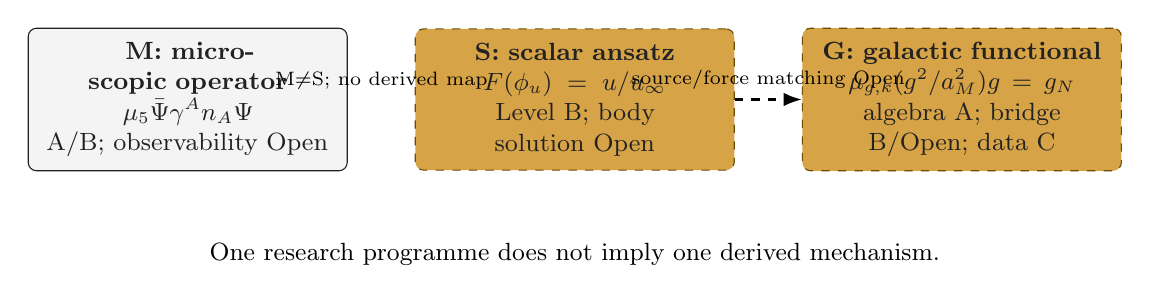
\begin{tikzpicture}[
  node distance=1.55cm and 0.85cm,
  box/.style={draw,rounded corners=3pt,align=center,inner sep=5pt,
              text width=3.7cm,minimum height=1.25cm,font=\small,
              text=ectInk},
  >=Latex]
\node[box,ectExternal] (M) {\textbf{M: microscopic operator}\\
$\mu_5\bar\Psi\gamma^A n_A\Psi$\\A/B; observability Open};
\node[box,ectOpen, right=of M] (S) {\textbf{S: scalar ansatz}\\
$F(\phi_u)=u/u_\infty$\\Level B; body solution Open};
\node[box,ectOpen, right=of S] (G) {\textbf{G: galactic functional}\\
$\mu_{g,k}(g^2/a_M^2)g=g_N$\\algebra A; bridge B/Open; data C};
\path (M) -- node[above,font=\scriptsize]{M$\neq$S; no derived map} (S);
\draw[->,thick,dashed] (S) -- node[above,font=\scriptsize]{source/force matching Open} (G);
\node[align=center,font=\small,below=0.8cm of S]
{One research programme does not imply one derived mechanism.};
\end{tikzpicture}
\caption{Status-sensitive separation of the fifth-force and galactic
objects.  M$\neq$S follows from variable/operator content.  The dashed
S$\to$G arrow is the missing physical-coordinate, source, force and
normalisation match.  The Level-C HRC algebraic diagnostic is not derived by the
microscopic operator or the Level-B scalar identities.  Gray denotes an
external/supplied operator and orange dashed boxes denote Open matching
routes; the text and border styles preserve the distinction in grayscale.}
\label{fig:ordered_branch_two_sectors}
\end{figure}
\FloatBarrier

\paragraph{Open completion.}
Higher-order terms may connect M and S, and a future body/source calculation
may connect S to G.  Those are independent Open gates.

\subsection{Gauge-sector summary, structural synthesis, and the open programme}
\label{sec:gauge_summary}

\textit{Status separated.  P5 is a medium/redundancy motivation, not a
derivation of local $U(1)$ or $SU(2)$ gauge dynamics.  Global compact-phase
Noether algebra and $\mathfrak{so}(3)\cong\mathfrak{su}(2)$ are exact in
their supplied models.  Local bundles, gauge-volume reduction, connections,
kinetic coefficients, an unbroken photon, physical matter representations,
charges, couplings, colour and electroweak identification remain
conditional/Open.  The director--fermion operators are allowed basis terms
only; their Wilson coefficients may vanish and their observable map remains
Open.}

\paragraph{What Section~\ref{sec:gauge_and_fifth} has established.}
After the introduction of the medium-character postulate~P5,
Section~\ref{sec:gauge_and_fifth} establishes the following hierarchy of results:
\begin{enumerate}[label=(\roman*)]
  \item The compact-phase $U(1)$ construction
    (Section~\ref{sec:u1_emergence}): a global Noether current is exact
    inside a supplied compact-phase EFT.  A local bundle, compensating
    connection and two-invariant ordered-background kinetic basis form a conditional completion;
    they do not follow from P5 alone.
  \item The non-Abelian orientation sector
    (Section~\ref{sec:nonabelian_embedding}): the ordered-branch
    orientation algebra gives the exact identity
    $\mathfrak{so}(3)\cong\mathfrak{su}(2)$, but the spacetime director
    is not an internal weak gauge field.  A local chiral bundle and
    connection require independent completion data.
  \item The electroweak-like embedding
    (Section~\ref{sec:ew_embedding}): a candidate
    $O(3)\to O(2)$ step gives a structural analogue of the
    weak-sector breaking pattern, but not a completed derivation of
    the physical electroweak sector~(Level~B/C).
  \item The matter-coupling architecture
    (Section~\ref{sec:matter_couplings}): Standard-Model-like
    interaction pattern reproduced at the EFT matching level.
  \item The candidate preferred-direction coupling
    (Sections~\ref{sec:fifth_coupling}--\ref{sec:fifth_to_galactic_bridge}):
    the displayed vector bilinear is allowed only in the stated restricted
    parity-even fermion EFT basis.  Its nonzero coefficient, sign, species
    dependence and observable bridge remain Open.
\end{enumerate}

\paragraph{Separation of spacetime and internal symmetries.}
The P4 direction datum carries a coordinate index of the Euclidean arena,
whereas internal gauge symmetries act on
multiplet indices of condensate components.
These sectors are therefore structurally distinct from the outset.
Section~\ref{sec:u1_emergence} records the additional assumptions needed to
complete the compact phase into a local $U(1)$ theory.  The construction is
conditional: the compact phase alone does not derive the bundle, reduced
Hessian, kinetic coefficients or physical matter map.

The Coleman--Mandula theorem~\cite{ColemanMandula1967} constrains the
structure of exact symmetries of a nontrivial relativistic S-matrix
under specific assumptions.
The present ECT discussion is formulated at the level of the condensate
action, the ordered branch, and the corresponding low-energy EFT
structures, prior to any full S-matrix reconstruction.
For that reason, the theorem does not by itself settle the viability of
the present embedding programme.
This should not be read as a circumvention of Coleman--Mandula, but as
a statement about the current level of analysis.

\paragraph{Connection to chirality and the matter sector.}
The exact decomposition $Spin(4)\simeq SU(2)_L\times SU(2)_R$ does not by
itself select a weak factor.  Fixing the ordered vector leaves the diagonal
stabiliser $SU(2)_{\rm diag}$, so the broken-phase geometry does not derive a
left/right matter asymmetry.  A physical chiral weak bundle, one-factor
vertex, coupling and matter representations must be supplied independently.

\paragraph{What P5 motivates and what remains open.}
P5 motivates looking for a local-redundancy completion but closes neither
the localisation step nor a physical gauge architecture.  The candidate
$SU(2)\times U(1)$ is therefore B/Open model building.  The open steps are:
\begin{enumerate}[label=(\roman*)]
  \item derive the local phase and internal-multiplet bundles, their
    gauge-volume quotients, connections and positive kinetic operators;
  \item identify an unbroken physical $U(1)_{\rm em}$ rather than a
    Higgsed connection, and derive its transverse state and metric;
  \item for $SU(3)$ colour, only the direct injective embedding in the
    displayed minimal algebra is excluded; P7 is an adopted Level-B structural postulate whose physical-colour map remains C/Open,
    while emergent/nonlinear, reducible/singlet, independent-bundle and
    defect-kernel routes and all physical colour owners remain Open;
  \item the coupling constants $(e,g,g',g_s)$ are not derived from
    condensate parameters;
  \item the candidate second transition $O(3)\to O(2)$ has not been
    derived dynamically from the bare action;
  \item the full Standard Model gauge sector, including anomaly
    cancellation and the correct matter representations, has not been
    reproduced.
\end{enumerate}
The corresponding Level~A programme for the ECT-specific preferred-
direction matter coupling is given separately in
Sections~\ref{sec:fifth_coupling}--\ref{sec:fifth_coefficient_constraints}.

\renewcommand{\arraystretch}{1.2}
\begin{longtable}{@{}L{6.8cm}L{2.2cm}L{5.5cm}@{}}
\caption*{\textbf{Status summary.}}\\[-4pt]
\toprule
Statement & Status & Comment \\
\midrule
\endfirsthead
\toprule
Statement & Status & Comment \\
\midrule
\endhead
\bottomrule
\endfoot
\multicolumn{3}{l}{\textit{Abelian compact-phase route}} \\
Global Noether current and current conservation
  & A & Strict within the compact phase EFT \\
Local phase redundancy
  & Open input & Not implied by global phase symmetry or P5 \\
Compensating connection and covariant derivative
  & A-math conditional & After a local bundle is supplied \\
Ordered-background kinetic basis $(I_1,I_2)$
  & A-math conditional / Open & Basis classification after bundle/director input; coefficients and physical Hessian Open \\
Compact holonomy and flux quantisation
  & A-math conditional & Requires consistent compact representation and connection \\
Photon identification
  & Open & Unbroken photon, charge/matter map and QED not derived \\
\multicolumn{3}{l}{\textit{Non-Abelian completion route}} \\
$\mathfrak{so}(3)\cong\mathfrak{su}(2)$
  & A & Strict Lie-algebra identity \\
Local internal multiplet redundancy
  & Open input & Carrier-space orientation triplet is not a gauge field \\
Ordered-branch $SU(2)\times U(1)$ gauge architecture
  & B/Open & Supplied model-building route, not derived \\
Non-Abelian EFT gauge completion
  & A-math conditional & Once the bundle and multiplet are supplied \\
$SU(3)$ direct-injective embedding no-go; P7 structural postulate
  & A restricted / Level-B input & Dimension excludes only direct injection;
    $SU(3)$ frame reduction is conditional A, while the physical-colour map
    and alternative microscopic origins remain Open \\
$O(3)\to O(2)$ as candidate weak-like step
  & B & Reduced algebraic/counting analogue only \\
$v_2$ as electroweak matching scale
  & Constraint & If a second condensate transition exists \\
\multicolumn{3}{l}{\textit{Matter couplings and interaction architecture}} \\
Gauge couplings $(e,g,g',g_s)$
  & Matched & EFT matching parameters, not derived \\
Yukawa/matter-coupling structure
  & B/C & Embedded at the EFT level \\
Chiral selection of $SU(2)_L$
  & Open & Vector stabiliser is diagonal; independent one-factor vertex required \\
\multicolumn{3}{l}{\textit{ECT-specific matter-sector deformation}} \\
Preferred-direction operator
  $n_A\bar\Psi\gamma^A\Psi$
  & A-math conditional / physical Open & Basis classification only; axial competitors depend on assumptions \\
Dimensionful coupling $\mu_5$
  & A-math/Open & Dimension fixed; value, sign, scale and species law Open \\
M: $n_A$ operator $\neq$ S: $\phi_u$ scalar ansatz
  & A/B & Structural nonidentity only \\
S scalar ansatz $\to$ G HRC gravity map
  & Open & Source/force/normalisation matching missing \\
G supplied HRC static functional, bridge, and diagnostics
  & A / Open / C & In-model algebra / bridge / data layers \\
Coefficient derived from condensate microphysics
  & Open & Not yet completed \\
\bottomrule
\end{longtable}

Section~\ref{sec:gauge_and_fifth} therefore establishes a layered
inventory rather than a single derivation.  P5 motivates deformable relational
response but neither creates local gauge redundancy nor closes the bundle,
connection, action, state or matter-representation gates.

\paragraph{Interaction map of ECT at the present stage.}
At the present stage, ECT organises three interaction-completion programmes;
none is yet a physical interaction derived from P1--P6:
\begin{enumerate}[label=(\roman*)]
  \item \textbf{Electromagnetic route:} the compact coherent-phase
    sector supplies global compact-phase algebra.  A local redundancy,
    ordered-background gauge kinetic coefficients, matter charge and an unbroken physical photon require
    added completion data.
  \item \textbf{Weak-interaction route:} the ordered-orientation
    sector supplies a rotation algebra, not a local chiral
    $SU(2)\times U(1)$ gauge theory.  The weak bundle, fields,
    representations and coefficients remain Open.
  \item \textbf{Gravity completion route:} the scalar characteristic geometry is derived in its stated model, but at fixed $\alpha,\beta$ and tangent-director linear order about the homogeneous background the fixed director map has no linear TT/static-density vertex.  A supplied scalar--tensor/HRC action provides conditional response algebra; a physical tensor, universal metric and nonlinear gravity owner remain Open.
\end{enumerate}
By contrast, a colour $SU(3)$ sector is not derived within the present
minimal condensate framework; its absence sharply localises the
missing internal structure required for a complete interaction
unification.

\paragraph{Native derivation criterion.}
A fundamental interaction is \emph{native} in ECT if:
(a)~it arises from an ordered-branch redundancy or ordered-branch
tensor mode;
(b)~its leading low-energy EFT closure is fixed internally by the
postulate framework, up to explicit matching parameters and clearly
identified unresolved higher-order sectors;
(c)~it does not require importing an external gauge group or an
external background structure.
By this criterion no physical electromagnetic, weak, colour or gravitational
interaction is yet native in the strong derivational sense.  The compact
phase, rotation algebra and scalar principal tensor are conditional starting
points; all local gauge, chiral, charge/matter and tensor/source completions
remain Open.

\section{Elementary Particles and Field Excitations in ECT}
\label{sec:particles}

\textit{Status guide for this chapter.}
The material below spans three levels of rigour, organised into
three categories of excitations
(Section~\ref{sec:particle_structure}):
\begin{description}[leftmargin=3em,style=unboxed,noitemsep]
  \item[(i) Condensate-coordinate and candidate-excitation sectors (Level~A/B/Open).]
    Physical graviton: Open completion target; at fixed $\alpha,\beta$ and tangent-director linear order the fixed director image has no linear TT/static-density seed (Section~\ref{sec:graviton}); nonlinear, composite or additional-field vertices are not excluded.
    One longitudinal orientation coordinate $\chi$ (Level~A kinematics), with
    a one-mode physical interpretation only in a supplied reduced EFT
    (Level~B;
    Section~\ref{sec:particle_soft_orientation}).
    Homogeneous P3 radial coordinate $\sigma$, with
    $m_{\Phi,\mathrm{rad}}^2=2\mu^2$ inside P3 (Level~A conditional;
    Section~\ref{sec:radial_mode}); a P4 amplitude pole or particle remains
    Open.  The P3 radial coordinate and the strict orientation-coordinate map
    have different owners; physical P4 amplitude and $\chi$ modes and a
    graviton require additional actions and reductions.
  \item[(ii) Conditionally supplied SM-like EFT embeddings (Level~B/C/Open).]
    Candidate gauge fields in separately supplied local-bundle completions
    (Section~\ref{sec:gauge_particles}; full development in
    Section~\ref{sec:gauge}).
    Higgs boson reinterpreted as secondary radial mode
    (Section~\ref{sec:ew_particles}).
    Fermions: structural reconstruction on the ordered branch
    (Section~\ref{sec:fermion_particles}; full development in
    Section~\ref{sec:fermions}).
    Neutrino sector: seesaw-type embedding
    (Section~\ref{sec:neutrino_particles}).
    These assume Standard-Model structure as external input;
    the SM gauge group, Yukawa couplings, and generation structure
    are not derived from the minimal bosonic condensate action.
  \item[(iii) Topological and conditional sectors (A-math conditional / physical Open).]
    Abstract texture/skyrmion classes of the supplied target are classified by
    $\pi_3(S^3) = \mathbb{Z}$, with
    $\pi_0 = \pi_1 = \pi_2 = 0$; conditional secondary defects
    (Section~\ref{sec:predicted_states}).
    Physical finite-action configurations, stability, masses and abundances
    require a configuration/action/transition owner and remain Open.
\end{description}

\noindent
One candidate fermion deformation allowed in the restricted ordered-branch
EFT is the director operator
$\mu_5\,\bar\Psi\gamma^A n_A\Psi$
(Section~\ref{sec:fifth_force_fermion}).
A condensed overview with status table is given in the chapter
summary~(Section~\ref{sec:particle_summary}).

\subsection{General Structure of Particle Excitations}
\label{sec:particle_structure}

\textit{Status: structural roadmap for the particle chapter.
This subsection does not yet derive the full particle content of nature.
Its purpose is to classify which coordinates or candidate excitations occur in
the supplied ordered-gradient chart, which sectors are only structurally embedded
at the EFT level, and which states are topological or conditional.
The strongest outputs of this chapter are therefore not the full
Standard Model particle spectrum, but the clear separation between exact
coordinate content, conditional condensate modes, embedded matter sectors, and
conditional
topological states.}

In the scalar-only ECT basis the fundamental degree of freedom
is the condensate field $\Phi$.
The orientation field $n_A$ is introduced only as a derived
ordered-branch variable through $Q_A = \partial_A\Phi = u\,n_A$
and is not an independent microscopic field in the present
formulation~(Section~\ref{sec:sector_map}).
Candidate particles and field excitations are organised as condensate
coordinates, fields in separately supplied internal/spinorial structures,
or maps into declared topological targets.  Their physical poles, state
spaces and configuration owners must be established separately.

\paragraph{Why a particle chapter is justified at all.}
The transition from Part~I to the present chapter is not a change of
subject, but a change of level of description.
Part~I analysed the supplied ordered chart, its conditional sector
decomposition, its scale inventory, and gauge-side structural embeddings.
Section~\ref{sec:particles} asks what these declared structures permit when read at
the level of particle-like excitations.
The chapter is therefore not an additional postulate about particles,
but the excitation-level inventory of the proposed condensate architecture.

\paragraph{What is meant here by a ``particle''.}
In the present ECT framework, ``particle'' does not always mean a
fundamental microscopic field inserted into the bare action.
Depending on the sector, it may instead refer to:
(i)~a required fluctuation mode of the ordered condensate,
(ii)~an EFT field structurally accommodated by internal symmetries of
the condensate background,
or (iii)~a map into a supplied topological target, with physical
configuration status still Open.
This distinction is essential for interpreting the status labels used
throughout this chapter.

\paragraph{Three categories of excitations.}
The particle content discussed in this chapter falls into three
categories with different derivation status:

\emph{(i) Condensate coordinates and candidate excitations.}
These statements have different status and must not be conflated:
\begin{itemize}
  \item homogeneous P3 amplitude coordinate with
    $m_{\Phi,\mathrm{rad}}^2=2\mu^2=2\lambda\phi_0^2$; its numerical
    mass and a physical P4 amplitude pole are Open
    (Section~\ref{sec:radial_mode});
  \item one longitudinal scalar coordinate $\chi$ from the
    integrability-constrained orientation map; its physical one-mode reduced
    EFT is conditional
    (Section~\ref{sec:particle_soft_orientation});
  \item physical graviton as an Open tensor-completion target; the displayed director map is not a helicity-2 owner (Section~\ref{sec:graviton}).
\end{itemize}

\emph{(ii) Conditionally supplied Standard-Model-like EFT embeddings.}
These may be accommodated on the ordered background but are not derived
from P1--P6:
\begin{itemize}
  \item candidate gauge fields in supplied local bundles motivated by
    compact-phase and rotation algebras
    (Section~\ref{sec:gauge_particles});
  \item electroweak-like gauge embedding and the associated secondary
    condensate sector (Section~\ref{sec:ew_particles});
  \item fermions as spinorial excitations compatible with the ordered
    background (Section~\ref{sec:fermion_particles});
  \item neutrino sector (Section~\ref{sec:neutrino_particles}).
\end{itemize}

\emph{(iii) Topological sectors and other conditional states.}
These are abstract target-space classifications or depend on a
possible second transition:
\begin{itemize}
  \item abstract texture/skyrmion classes from $\pi_3(S^3) = \mathbb{Z}$
    and vanishing lower homotopy groups
    $\pi_0 = \pi_1 = \pi_2 = 0$ for the supplied target;
  \item (conditional) secondary defects from $\pi_2(S^2)$ if
    $O(3)\to O(2)$ exists;
  \item the Higgs-like secondary radial mode $h$ as the
    \emph{conditional particle-level interpretation} of the secondary
    condensate sector, if the weak-like $O(3)\to O(2)$ transition is
    realised.
\end{itemize}
Topological sectors are developed in
Section~\ref{sec:predicted_states}, while the conditional Higgs-like
reinterpretation is discussed primarily in
Section~\ref{sec:ew_particles}.

\paragraph{Classification criterion.}
The division into the three categories above is not merely descriptive.
It reflects three distinct logical relations to the ECT foundation:
\begin{itemize}
  \item a coordinate is \emph{kinematically required} if it follows from
    the supplied parametrisation itself; physical propagation still requires
    an owned action, domain and state;
  \item a state is \emph{embedded} if it can be consistently realised in
    the ECT low-energy framework but is not derived from P1--P6;
  \item a state is \emph{conditional or topological} if it depends on
    the topology of a supplied target or on an additional transition
    not yet established from first principles.
\end{itemize}
These three classes therefore correspond not merely to different kinds
of excitations, but to different logical relations to the foundation of
ECT: strict consequence, EFT embedding, and conditional/topological
realisation.

\paragraph{Physical interpretation and condensed-matter analogy.}
The three categories have direct analogues in condensed-matter physics.
Category~(i) coordinates are analogous to the variables used to describe
phonons in a crystal, but the analogy does not prove an ECT pole: an ordered
physical medium, its quadratic action and state would first have to exist.
Category~(ii) fields are analogous to \emph{impurity atoms in a
crystal lattice}: they are compatible with the medium and respect its
symmetries, but they are not derived from the lattice structure alone.
Category~(iii) states are analogous to \emph{topological defects}
(dislocations, vortices): their possible topological protection is
classified by the homotopy of a declared target, while physical existence,
finite action and abundance depend on dynamics and boundary conditions.

\paragraph{Comparison with quantum field theory.}
In standard QFT, particles are postulated as quanta of independent
fields ($\phi$, $A_\mu$, $\psi$,~\ldots) defined on a fixed
spacetime background.
Each field carries its own Fock space.
The architecture does not place all candidate sectors on the same logical
footing.  Category~(i) contains condensate coordinates and fluctuations that
arise in the supplied broken-branch parametrisation; their physical poles,
states and particle interpretation still require the corresponding actions,
domains and projectors.  Category~(ii) fields are structurally embedded in
the condensate symmetry architecture but are not derived from the minimal
scalar action.  Category~(iii) consists of maps into the supplied
target~$S^3$; topology fixes abstract sector labels and non-protection
statements, not stable particles, masses or abundances.  The vanishing groups
$\pi_2$, $\pi_0$ and $\pi_1$ are exact for that target.  Turning them into
physical exclusions of monopoles, walls or strings requires identifying it
with the complete physical vacuum/configuration space, which remains Open.

\paragraph{Particle scales versus the galactic fit length.}
The particle discussion contains the exact P3 relation
$m_{\Phi,\mathrm{rad}}=\sqrt{2\lambda}\phi_0$, an Open and distinct
P4 pole, the conditional secondary scale $m_h\sim v_2\approx246$\,GeV, and
the separately classified longitudinal coordinate $\chi$ with its
conditional reduced-EFT mode interpretation.  The
kpc quantity $L_{\rm gal}$ is not a particle or condensate
mass scale; it is a conditional HRC matching length whose ECT and scalar/AQUAL matching
remain Open.

\paragraph{Dependence on earlier results.}
The present classification relies on four earlier structural results of
Part~I:
the broken-phase sector map of Section~\ref{sec:broken_spectrum},
the dimensionally separated scale inventory of Section~\ref{sec:three_scales},
the branching architecture of Section~\ref{sec:branching},
and the gauge-sector embedding analysed in
Section~\ref{sec:gauge_and_fifth}.
Section~\ref{sec:particles} should therefore be read not as an independent particle
postulate, but as the particle-level unpacking of those earlier
structural ingredients.

\paragraph{What this chapter does not claim.}
The present chapter does not claim that the full Standard Model particle
spectrum has been derived from the minimal scalar condensate action.
In particular, the gauge group, Yukawa hierarchy, generation structure,
and the detailed fermion spectrum remain beyond the present Level~A
closure.
What is established here is a structured map of which sectors already
follow from the ordered branch, which are admissible EFT embeddings,
and which remain conditional or open.

\paragraph{Dependence on later parts of the paper.}
Section~\ref{sec:particles} identifies particle-like sectors and their derivational
status, but it does not by itself complete the full phenomenological or
cosmological role of those sectors.
Questions of macroscopic closure, dark-sector behaviour, and late-time
observational consequences are deferred to the later parts of the paper.
This prevents the particle classification from being overinterpreted as
a complete physical model already at the level of Part~I.

The purpose of the following subsections is therefore not merely to
list possible excitations, but to determine which particle-like sectors
already belong to the broken condensate branch itself, which require
additional EFT embedding, and which remain conditional on topology or a
secondary transition.
In this sense, the chapter is a derivation-status map of the ECT
particle sector, not a claim of complete particle unification.
Its organising principle is not phenomenological completeness, but
logical dependence on the ordered-branch foundation.

\paragraph{Multi-particle description: why it is necessary and how ECT
differs from QM and QFT.}
Ordinary non-relativistic quantum mechanics operates on a Hilbert
space~$\mathcal{H}_N$ of fixed particle number~$N$.
Processes with variable~$N$ (photon emission, pair creation,
annihilation) require quantum field theory, where the Fock space
$\mathcal{F}=\bigoplus_{N=0}^{\infty}\mathcal{H}_N$ and
creation/annihilation operators are introduced as additional postulates.
In ECT the architecture is different: fundamental are not ``individual
particles'' but configurations of a single condensate field~$\Phi$.
Changing particle number is a reconfiguration of the same medium,
analogous to the appearance and disappearance of vortices in a
superfluid.

Multi-particle description remains necessary for coherent and
decohering regimes alike.  Coherent many-body interaction occurs within the
ordered Lorentzian dynamics; it does not require a large record exponent or a
change of metric signature.  Four independent reasons are:
\begin{enumerate}[label=(\alph*)]
  \item \emph{Entanglement:} a supplied nonfactorising state/channel requires
    a many-body description; a common condensate alone does not force it
    (Section~\ref{sec:qs_entanglement});
  \item \emph{Exchange statistics:} for the separately supplied defect-free
    $\mathbb R^3$ identical-point configuration space, the topology
    ($\pi_1(\mathcal{M}_2)=\mathbb{Z}_2$) supplies two exchange homotopy
    classes; the physical spatial slice, excitation map, representation and
    spin--statistics map remain Open (Section~\ref{sec:qs_statistics});
  \item \emph{Decoherence channels:} a rate is protocol-, state-, coupling-
    and spectrum-dependent; no universal $1/(N_{\rm eff}\gamma)$ law follows;
  \item \emph{Variable excitation number:} pair creation, annihilation and
    radiation require a Fock/sector completion.  Particle production at the
    $O(4)\to O(3)$ ordering event additionally requires a nonequilibrium
    transition history and is not yet derived.
\end{enumerate}

\paragraph{Status of Fock space.}
ECT does not require Fock space as a fundamental postulate.
However, an explicit emergent sector decomposition with variable
excitation number---especially for the fermionic many-body
sectors---remains to be constructed from condensate dynamics.
This is a nontrivial reconstruction problem rather than a foundational
gap~(Open; OP-Q11).


\subsection{Soft Orientation Sector of the Condensate}
\label{sec:particle_soft_orientation}

\textit{Status: minimal orientation EFT is Level~B.
Three independent physical Goldstone particles are \textbf{not} claimed
in the present scalar-only basis; see Section~\ref{sec:goldstone_integrability_main}
and Appendix~\ref{app:goldstone_integrability}.}

\paragraph{Why this coordinate sector is considered.}
A supplied nonzero P4 vector has stabiliser $O(3)$ and abstract orientation
orbit $O(4)/O(3)\simeq S^3$.  This conditional group geometry motivates an
orientation-coordinate sector, but does not prove a physical vacuum manifold
or propagating mode.
What is nontrivial in scalar-only ECT is that the strict gradient map has much
smaller independent coordinate content than naive broken-generator
counting would suggest.  The number of physical propagating modes follows
only after a reduced action, constraint quotient/domain and projector are
supplied.
For this reason, the soft orientation sector belongs to the class of
condensate-coordinate and candidate-excitation sectors introduced in
Section~\ref{sec:particle_structure}; its physical particle content is not
fixed by integrability alone.

\paragraph{Minimal conditional chain.}
The orientation-coordinate analysis uses three successive facts:
(i)~a supplied nonzero vector has $O(3)$ stabiliser and abstract orbit
$O(4)/O(3)\simeq S^3$;
(ii)~naive broken-generator counting therefore suggests three soft
directions;
(iii)~in the strict scalar-only basis, the order parameter is generated
by a single exact one-form $Q_A=\partial_A\Phi$, so the kinematically
independent soft-coordinate content is reduced to one longitudinal
scalar~$\chi$.
The orbit geometry is exact conditional mathematics, whereas its
identification with a physical sector and its particle-like content remain
Open/conditional on supplied reduced dynamics.

A supplied nonzero vector has $O(3)$ stabiliser, so its orientation orbit is
\begin{equation}
  O(4)/O(3)\simeq S^3.
\end{equation}
In a generic internal-symmetry breaking this would yield three
independent Goldstone bosons.
However, in the present scalar-only ECT basis the ordered quantity is
$Q_A=\partial_A\Phi$, which is an exact one-form.
The integrability constraint $\partial_A Q_B-\partial_B Q_A=0$ implies
that the orientation triplet reduces kinematically to one longitudinal
scalar coordinate~$\chi$ at linear order~\cite{Ivanov1975,McArthur2010}:
\begin{equation}
  \pi_i = \frac{1}{u_0}\partial_i\chi, \qquad \sigma = \partial_w\chi.
\end{equation}

\paragraph{Minimal orientation EFT.}
A three-component orientation parametrisation of $S^3$ remains a useful
effective language for the supplied chart, but it should be understood
as a minimal EFT organisation, not as three independent propagating
particles.
The broken-generator counting $\dim O(4)-\dim O(3)=3$ is a
geometric statement; the strict scalar map has one independent
longitudinal coordinate at linear order.  A supplied reduced EFT may then
realise $N_G^{\rm phys}=1$ (Level~B), but integrability alone does not prove
that physical count.

\paragraph{Three levels of statement.}
It is important to distinguish:
\begin{enumerate}[label=(\roman*)]
  \item the \emph{geometric} statement that the supplied nonzero vector has
    an $S^3$ orientation orbit;
  \item the \emph{group-theoretic} statement that
    $\dim O(4)-\dim O(3)=3$;
  \item the \emph{conditional physical} statement that a supplied reduced
    EFT with the required domain and projector promotes the one longitudinal
    coordinate to one independent propagating soft mode at linear order.
\end{enumerate}
The first two statements and the coordinate reduction are strict conditional
mathematics; the third is Level~B and supplies a particle interpretation only
inside its declared reduced EFT.  Physical SSB and identification of the
orbit with the complete vacuum manifold remain Open.
Confusion between these three levels is precisely what leads to the
incorrect ``three physical Goldstones'' reading: the present scalar-only map
does not contain three independent coordinates, while a larger physical mode
bundle is not derived.

\paragraph{Mass status of the longitudinal scalar coordinate.}
The supplied derivative-only reduced EFT used for the linear soft-dispersion
benchmark contains no $\chi^2$ term and therefore has $m_\chi=0$ inside that
declared truncation.  This is a conditional property of the displayed kernel,
not a deduction of a physical zero from P1--P6.  The spacetime/gradient
integrability reduction is kinematic: it supplies neither an internal shift
symmetry nor a regulator-compatible Ward identity that protects the physical
mass.  Potential, constraint, radiative, boundary or additional-field terms
may change the reduced Hessian.  Conversely, an exact zero would become
protected only after an owned stationary action, domain, constrained projector
and counterterm-closed identity are given.  None is presently available, so
the physical $m_\chi^2$, its sign and its radiative stability are
\texttt{NOT IDENTIFIABLE} / Open (OP-GM).  A pseudo-Goldstone mass is one
possible conditional deformation, not the only logically admissible mass
owner.

\paragraph{Named optional soft-scalar hypotheses.}
One C/Open completion may supply a shift-compatible derivative operator whose
dimensionless momentum-space coupling is
\begin{equation}
 g_\chi(k)=c_\chi\frac{k}{f_\chi},
 \qquad f_\chi>0,
 \label{eq:soft_scalar_derivative_hypothesis}
\end{equation}
with independent coefficient $c_\chi$ and scale $f_\chi$; the optional match
$f_\chi=\phi_0$ is a further input.  A distinct named scale hypothesis is
\begin{equation}
 \begin{gathered}
 H_0^{(\mathrm{freq})}>0,
 \qquad H_{0,E}:=\hbar H_0^{(\mathrm{freq})},
 \qquad \zeta_H>0,\\
 m_{\chi,E}:=m_\chi c^2=\zeta_H H_{0,E},
 \qquad \xi_\chi=\frac{\hbar c}{m_{\chi,E}}
 =\frac{c}{\zeta_HH_0^{(\mathrm{freq})}}.
 \end{gathered}
 \label{eq:hubble_soft_scalar_hypothesis}
\end{equation}
where $\zeta_H$ is a supplied positive coefficient and may differ from
unity.  The separate boundary choice $\zeta_H=0$ is a massless branch with
$\xi_\chi=\infty$ only as a limit; the displayed quotient is not used there.  Neither branch is
selected by P1--P6.  They derive no abundance, dark-matter/dark-energy role,
HRC map or laboratory signal without the action, state, source and observable
owners.

For scale orientation only, the explicit point
$\zeta_H=\zeta_\phi=1$,
$\phi_0^{\rm bench}=\bar M_{\rm Pl}=2.4353\times10^{18}\,\mathrm{GeV}$ and
$H_0^{(\mathrm{freq})}=70\,\mathrm{km\,s^{-1}\,Mpc^{-1}}$ gives
\begin{equation}
 \begin{gathered}
 m_{\chi,E}^{\rm bench}=1.493\times10^{-33}\,\mathrm{eV},
 \qquad
 \xi_{\chi}^{\rm bench}=1.322\times10^{26}\,\mathrm{m},\\
 \dfrac{m_{\chi,E}^{\rm bench}}{\phi_0^{\rm bench}}
   =6.131\times10^{-61}.
 \end{gathered}
 \label{eq:hubble_soft_scalar_unit_benchmark}
\end{equation}
Here $\xi_{\chi}^{\rm bench}=c/H_0^{(\mathrm{freq})}$ is a reduced-Compton
proxy; a physical
correlation length still requires an owned propagator.  These values are
Level~C consequences of the displayed parameter point, not
ECT predictions, evidence, or an identification of~$\chi$ with a dark-sector
component.  Nor do these scale conversions establish a numerical decoupling
conclusion.

\paragraph{Soft-sector role versus the HRC no-halo algebraic diagnostic.}
The Level-C HRC algebraic diagnostic is evaluated on selected benchmarks without a
particle-halo or Goldstone component in that diagnostic model.  This is a
phenomenological choice, not an architectural proof that the soft orientation
sector or particle dark matter is absent.  The mass, couplings, abundance and
independent cosmological role of any physical mode represented by $\chi$
remain Open.


\paragraph{Role in the candidate-state inventory.}
The scalar coordinate $\chi$, together with its conditional one-mode reduced
EFT interpretation, is listed as item~(ii) in the inventory beyond the
observed SM spectrum (Section~\ref{sec:predicted_states}).  It is not a derived
ECT particle; its mass, couplings, stability and possible cosmological
abundance remain Open.

This concludes the softest condensate sector of the particle chapter.
The next subsections turn to heavier or more structurally elaborate
excitations, beginning with the radial condensate mode.

\renewcommand{\arraystretch}{1.2}
\begin{longtable}{@{}L{6.7cm}L{2.2cm}L{5.6cm}@{}}
\caption*{\textbf{Status summary.}}\\[-4pt]
\toprule
Statement & Status & Comment \\
\midrule
\endfirsthead
\toprule
Statement & Status & Comment \\
\midrule
\endhead
\bottomrule
\endfoot
Orientation-coordinate sector motivated by the supplied orbit
  & A-math/B/Open & Orbit geometry and scalar-coordinate reduction are
    conditional mathematics;
    physical propagation needs a supplied reduced action/domain/projector \\
Supplied nonzero vector has $O(3)$ stabiliser and $S^3$ orbit
  & A-math conditional / physical SSB Open & Group geometry only \\
Naive Goldstone counting: $\dim O(4) - \dim O(3) = 3$
  & A & Broken-generator counting \\
Integrability gives one longitudinal scalar coordinate; a supplied reduced
  EFT may have $N_G^{\rm phys} = 1$
  & A kinematics / B physical & Physical count additionally requires the
    action, quotient/domain and projector; see
    Appendix~\ref{app:goldstone_integrability} \\
Supplied derivative-only $\chi$ kernel has $m_\chi=0$
  & A-math conditional / B as ECT model & Property of the declared truncation, not of P1--P6 alone \\
Optional $H_\chi$ scale
$m_{\chi,E}=\zeta_H H_{0,E}$
  & C/Open input & Supplied positive $\zeta_H$; the $\zeta_H=0$ boundary is
    massless; no abundance, dark-sector role or signal follows \\
Physical $m_\chi^2$ and protection mechanism
  & Open (OP-GM) & Stationary owner, projector, Ward identity and radiative closure missing \\
Physical soft-mode mass, operator and abundance
  & Open & No numerical infrared scaling or cosmological identification is retained \\
Soft-mode dark-matter interpretation
  & Not claimed & The HRC diagnostic omits a soft-mode component; its
    abundance, galactic role and S$\to$G matching remain Open \\
\bottomrule
\end{longtable}

\subsection{Radial Condensate Mode}
\label{sec:radial_mode}

\textit{Status: three distinct owners.
The homogeneous P3 potential has a Level-A conditional amplitude coordinate
with curvature $m_{\Phi,\mathrm{rad}}^2=2\mu^2$.  P4 instead postulates a
gradient-ordered background; its amplitude coordinate, stationary action,
constrained Hessian, pole and correlation length are Open.  Equality of a
future P4 pole with the P3 curvature is only a matching hypothesis.  A
separately supplied electroweak-like second condensate may contain a
Higgs-like radial mode at Level~C/Open and is neither the P3 coordinate nor a
derived P4 particle.}

\paragraph{What is required and what is not.}
For the homogeneous P3 extrema, decomposing fluctuations of the scalar
amplitude is standard and unavoidable; the local curvature defines the P3
radial coordinate.  This statement does not transfer to the independent P4
gradient datum.  A physical P4 amplitude excitation exists only if a
stationary P4 action and its physical fluctuation reduction produce a pole.
It is therefore currently an Open candidate-excitation sector in the
classification of Section~\ref{sec:particle_structure}.

\paragraph{Contrast with the soft orientation sector.}
The scalar coordinate $\chi$ of
Section~\ref{sec:particle_soft_orientation} parametrises a supplied linear
orientation map.  A normal P4 amplitude coordinate would be distinct from
$\chi$, but neither its kinetic term nor its pole is present in the displayed
P4 data.  The P3 homogeneous amplitude is a different owner again.  Thus no
current result identifies a heavy P4 mode or the breakdown scale of the
broken-phase P4 EFT; each physical spectrum requires its declared action and
Hessian.

\paragraph{Minimal owner chain.}
P3 supplies a scalar action, homogeneous extrema and their local Hessian, so
its amplitude curvature is calculable.  A tangential/normal decomposition
about P4 would first require the P4 configuration to be stationary for an
owned constrained action.  The postulated gradient profile is generally not
stationary for the P3 action.  Therefore a P4 radial pole, its physical scale
and any role as a P4 ultraviolet threshold remain Open rather than following
from the existence of a nonzero ordered datum.

\paragraph{Tangential versus normal coordinates.}
For a supplied stationary broken-phase action, tangential and normal
coordinates are geometrically inequivalent.  Geometry alone, however, does
not determine their kinetic operators, pole residues or masses.  In the
current P4 programme the orientation coordinate is a conditional reduction
and the normal amplitude pole is Open; calling the latter heavy would assume
the missing Hessian.

\paragraph{First owner: homogeneous P3 amplitude fluctuation.}
For the P3 scalar action, write
$\Phi=\phi_0+\delta\Phi$ about either homogeneous minimum.  Its local
curvature is exactly
\begin{equation}
  m_{\Phi,\mathrm{rad}}^2:=V''(\phi_0)
  =2\mu^2=2\lambda\phi_0^2 .
  \label{eq:sigma_mass_radial}
\end{equation}
This is a classical homogeneous-P3-minimum result.  It is not the pole of the P4
gradient amplitude in
$\partial_A\Phi=(u_0+\sigma)n_A$: that pole needs a stationary P4 action,
constraints and Hessian.  The exact P3 mass is
\begin{equation}
  m_{\Phi,\mathrm{rad}}=\sqrt{2\lambda}\,\phi_0 .
  \label{eq:sigma_planck}
\end{equation}
The value of $\lambda$ is not selected, so matching $\phi_0$ alone does not
fix a Planck-scale mass.  This is not a derived P4 particle or a P4 EFT
threshold.  It is also distinct from the supplied
secondary electroweak Higgs-like candidate.

The positivity $V''(\phi_0)>0$ gives tree-level local stability of
the homogeneous P3 amplitude coordinate within the stated potential.  It
does not establish stability of the P4 gradient background.
The one-loop vacuum stability analysis, the question of false vacuum
and Coleman vacuum decay, and the comparison with Standard-Model
electroweak metastability are developed in
Section~\ref{sec:vacuum_stability}.

\textbf{Spin and propagation.}
The P3 amplitude coordinate is scalar under the Euclidean rotations of its
own action.  A Lorentzian P4 particle interpretation, pole, residue and
propagation cone are Open until the P4 action and continuation are supplied.
Equality with matter, photon and tensor cones is likewise not derived.

\paragraph{Why the P3 radial coordinate is distinct from the soft
orientation coordinate.}
The homogeneous-P3 radial coordinate $\sigma$ must also be distinguished from the
longitudinal scalar coordinate $\chi$ of the orientation sector
(Section~\ref{sec:goldstone_integrability_main}).
This distinction is ECT-specific and follows from the integrability of
the gradient condensate: $Q_A=\partial_A\Phi$ is an exact one-form,
so amplitude and orientation fluctuations are not independent generic fields.
At coordinate level, a putative $\sigma$ would vary
$|Q_A|=|\partial_A\Phi|$, whereas $\chi$ parametrises the supplied
longitudinal orientation variation.  They are distinct coordinates, but
coordinate separation is not a two-pole theorem.  Their physical mode content
requires separate reduced actions; the $\chi$ model is conditional and the P4
amplitude pole remains Open.

\paragraph{Conditional higher-dimension expansion.}
If a positive isolated P4 pole is later derived and couples locally to the
retained fields, standard EFT matching may generate
\begin{equation}
  \Delta\mathcal{L}_{\rm EFT}
  \sim \sum_{n\ge 1}
  \frac{\mathcal{O}_{2n+4}}{m_{\rm P4,pole}^{2n}} .
  \label{eq:HDO_sigma}
\end{equation}
This is a conditional decoupling template, not a current P4 result.  The P3
homogeneous curvature may analogously set a threshold only for a supplied EFT
built about that chosen classical P3 minimum; it cannot be imported
into P4 without matching.  A physical quantum vacuum still requires its
state and infinite-volume or boundary/source-limit owner.


\paragraph{What is strict and what is not.}
Strictly, the homogeneous P3 action has the curvature
$m_{\Phi,\mathrm{rad}}^2=2\mu^2$.  A P4 radial pole and ultraviolet
threshold do not follow from P4's nonzero gradient datum.  The secondary mode
at $v_2$ is separately conditional on the supplied weak-like transition.

\paragraph{Conditional bridge to the candidate action coefficient.}
The supplied fixed-core phase closure contains
\begin{equation}
  \iota_0^{\rm EFT} = \frac{c_\perp\,K_\theta}{2\,m_\varphi^{2}}.
  \label{eq:S0_sigma_bridge}
\end{equation}
The displayed $\iota_0^{\rm EFT}$ formula is dimensionless and exact
inside the supplied reduced closure.  Identifying its core parameter with the
P3 mass, $m_\varphi=m_{\Phi,\mathrm{rad}}$, or with a future P4 pole is an
additional matching ansatz.  A physical action further requires
$S_{0,\rm phys}=\Sigma_\theta\iota_0^{\rm EFT}$.  Neither the loop functional
nor P3 derives a P4 threshold, the fixed-core data or a common physical owner;
the bridge remains Level-B/Open.

\paragraph{P3 radial correlation and the Open P4 threshold.}
For the homogeneous P3 action, the Gaussian amplitude coordinate has
$m_{\Phi,\mathrm{rad}}^2=2\mu^2$.  Its Euclidean propagator has the
large-distance form
\begin{equation}
  G_{\Phi,\mathrm{rad}}(r)
  \;\propto\;
  \frac{e^{-m_{\Phi,\mathrm{rad}}r}}{r^{3/2}}
  \qquad (r\to\infty),
  \label{eq:G_sigma_decay}
\end{equation}
so $\xi_{\rm P3}=m_{\Phi,\mathrm{rad}}^{-1}$ is the P3 correlation length.
This result does not provide a propagating pole, range or cutoff for the
independently postulated P4 gradient background.

\paragraph{P4 EFT-threshold programme.}
\label{par:uv_threshold}
A physical P4 breakdown threshold requires a stationary P4 action, its
constrained Hessian and a positive isolated pole
$m_{\rm P4,pole}$.  Those owners are not presently supplied, so
$m_{\rm P4,pole}$, $\xi_{\rm P4}=m_{\rm P4,pole}^{-1}$ and any P4
decoupling threshold are Open.  If such a pole is later derived, standard EFT
matching may use it as a conditional threshold.  Identifying it with
$m_{\Phi,\mathrm{rad}}$ is a separate matching hypothesis, not an identity.
Neither statement supplies a microscopic ultraviolet regulator or proves
that the full theory is ultraviolet complete.

\paragraph{Connection to the quantum-gravity programme.}
The P3 amplitude scale, a future P4 pole and the physical action-unit
programme are distinct owners.  No current theorem turns the P3 correlation
length into a gravity cutoff or a universal action quantum.  A completed P4
action could later provide a pole and a controlled EFT domain; that result
would still require independent tensor, state and action-normalisation maps.

\paragraph{Status of the primary and secondary amplitude coordinates.}
A homogeneous P3 amplitude curvature exists conditionally in the supplied
P3 action.  The P4 decomposition supplies only an amplitude coordinate until
its stationary action and pole are derived.  Therefore no physical
``primary radial particle'' is required merely by P4 ordering.  A secondary
Higgs-like mode is even more conditional: it exists only inside a separately
supplied electroweak-like transition and field completion.  The two
coordinates, their actions and any mixing vertex must be independently
owned.

\paragraph{Second radial mode: candidate from the electroweak-like transition.}
If the second condensate transition $O(3)\to O(2)$ is realised at
scale $v_2$ (Appendix~\ref{app:second_transition}, assumptions A1--A2),
the effective broken-phase description at that scale admits a radial
fluctuation around the second condensate vacuum.
In an effective field theory language (\emph{not} a second independent
fundamental field, but an effective condensate sector at scale $v_2$):
\begin{equation}
  \phi_{\rm ew} = v_2 + h, \qquad
  m_h^2 = V_{\rm ew}''(v_2) = 2\lambda_2\,v_2^2,
  \label{eq:higgs_mass_candidate}
\end{equation}
where $\lambda_2$ is the quartic coupling of the second-condensate
effective sector at scale~$v_2$.

This mode is \emph{structurally analogous} to the Standard Model
Higgs boson in the following sense:
\begin{itemize}
  \item it is the radial excitation of the second-condensate VEV
    (formally analogous to the Higgs field);
  \item the spontaneous breaking of the internal symmetry at $v_2$
    would generate masses for the vector bosons of the embedded
    electroweak-like gauge sector, if a local gauge realisation exists
    (formally analogous to the Higgs mechanism);
  \item the relation $m_h = \sqrt{2\lambda_2}\,v_2$ has the same
    structure as the SM Higgs mass formula.
\end{itemize}

\paragraph{Honest status of the Higgs-like mode.}
Three levels must be distinguished:
\begin{enumerate}
  \item \textbf{Level B/C (structural):} if the second transition
    exists and if the corresponding $O(3)$-sector admits a local
    gauge realisation (not implied by P1--P6; part of OP-EW),
    a radial mode $h$ at scale $v_2\approx246$\,GeV is structurally
    present.
  \item \textbf{Matching constraint:} the PDG-2025 review quotes the
    ATLAS Run-1+Run-2 diphoton-plus-four-lepton combination
    $m_H=125.11\pm0.09\,({\rm stat})\pm0.06\,({\rm syst})$\,GeV
    ~\cite{ParticleDataGroup2025Higgs}.  Consistency with this external
    measurement would require $\lambda_2(v_2)\approx0.13$.
    This value is not derived from ECT postulates P1--P6; it is a
    matching input if one demands consistency with the measured Higgs mass.
  \item \textbf{Open (OP-EW):} the dynamical mechanism producing
    $v_2$, the origin of $\lambda_2$, and the localisation of the
    $O(3)$ symmetry at scale $v_2$ are not derived from the minimal
    scalar condensate and remain open problems.
\end{enumerate}

\paragraph{Relation to the scale inventory.}
The P3 radial sector has the exact supplied-model relation
$m_\sigma=\sqrt{2\lambda}\phi_0$; its numerical mass and the distinct P4
pole remain Open.
Conditionally, the secondary sector has $m_h\sim v_2$.
The distinct kpc quantity $L_{\rm gal}$ is a conditional HRC matching
length used in Level-C diagnostics; assigning it to the amplitude sector requires the
still-Open scalar-to-galactic map.


\paragraph{Higgs self-coupling and testability.}
If the secondary condensate potential is quartic near $v_2$,
\begin{equation}
  V_{\rm ew}(\phi_{\rm ew})
  =
  \frac{\lambda_2}{4}\left(\phi_{\rm ew}^2-v_2^2\right)^2,
\end{equation}
then the Higgs mass satisfies
\begin{equation}
  m_h^2 = 2\lambda_2\,v_2^2,
  \qquad
  \lambda_2 = \frac{m_h^2}{2v_2^2}.
\end{equation}
The corresponding cubic self-interaction is
\begin{equation}
  V_{\rm ew} \supset \lambda_2\,v_2\,h^3,
\end{equation}
or equivalently
\begin{equation}
  V_{\rm ew}'''(v_2) = 6\lambda_2\,v_2 = \frac{3m_h^2}{v_2}.
\end{equation}
Different collider conventions for the trilinear Higgs coupling differ
by combinatorial factors; the expression above refers to the third
derivative of the effective potential at the minimum.
Deviations from this quartic relation would signal non-quartic
corrections to the effective potential at scale $v_2$---for instance,
induced by the primary condensate sector or by the dynamics of the
second transition itself.
Deviations from this quartic relation would indicate that the effective
secondary potential is not approximately quartic near its minimum, or
that additional condensate-sector corrections enter already at that
scale.
The present framework does not determine the size of such deviations.


\paragraph{Reframing the hierarchy problem.}
The usual SM hierarchy problem asks: why is the Higgs mass so small compared
to the Planck scale~\cite{tHooft1979}?
ECT recasts this as a condensate-spectrum question: why does a second
condensate branch appear at $v_2\sim 10^{-16}\,\phi_0$?
This is still an open problem~(OP-EW), but the reframing is itself meaningful:
instead of a fine-tuning of one scalar mass, the challenge becomes explaining
the dynamical origin of a second ordered phase at an intermediate scale.
The updated OP-EW-scale programme treats this hierarchy as a
non-polynomial scale-generation problem,
$v_2=\phi_0\,e^{-\mathcal{I}_{\rm EW}}$ with
$\mathcal{I}_{\rm EW}\approx36.8$
(Section~\ref{sec:three_scales}). Candidate mechanisms include
alignment running, walking/near-conformal dynamics, Miransky/BKT
scaling, and topological/Hopf-like routes
(Appendix~\ref{app:hopf_locking}). None is derived from P1--P6,
and none by itself solves the radiative stability problem of
the secondary radial mode.


\paragraph{Radiative stability: what ECT does and does not solve.}
The reframing of the hierarchy problem as a condensate-spectrum
question does not by itself resolve the radiative stability issue.
If the secondary radial mode $h$ couples to other fields (gauge
bosons, fermions) with generic EFT couplings, its mass receives
quadratic radiative corrections of order
\pagebreak[3]
\begin{equation}
  \delta m_h^2 \;\sim\;
  \frac{g^2}{16\pi^2}\,\Lambda_{\rm sec}^2 ,
  \label{eq:quadratic_correction}
\end{equation}
where $\Lambda_{\rm sec}$ is an independently supplied regulator or heavy
threshold of the secondary EFT.  This is a schematic Wilsonian sensitivity;
its coefficient and even its explicit quadratic form depend on the
regulator, couplings and field content.  Choosing
$\Lambda_{\rm sec}\sim\bar M_{\rm Pl}$ is a benchmark, not a result: neither
the P3 mass $m_\sigma$ nor an Open P4 pole is automatically the secondary
cutoff.
The resulting fine-tuning is of the same order as in the Standard Model.
ECT does not claim to solve this problem.
What it offers is a different \emph{physical context}:
the fine-tuning question becomes whether the dynamics of the
second condensate transition naturally selects $v_2 \ll \phi_0$.
A possible mechanism is dimensional transmutation via the
RG running of the effective quartic coupling from $\phi_0$ to $v_2$
(Section~\ref{sec:three_scales},
Appendix~\ref{app:second_transition}), but this remains
Level~C and has not been demonstrated within ECT.
Absent an additional symmetry, compositeness mechanism, or dynamical
selection principle, the secondary scalar remains quadratically
sensitive to the primary UV scale.
Any claim that ECT resolves the naturalness problem would be
premature.

\paragraph{Comparison with other Higgs frameworks.}

\emph{Standard Model Higgs:}
in the SM the Higgs is an elementary scalar doublet introduced
phenomenologically~\cite{EnglertBrout1964,Higgs1964}.
In ECT the P3 homogeneous radial coordinate is present in the supplied P3
model, while a physical P4 radial pole and the Higgs-like secondary mode both
require additional action owners; the latter is also conditional on the
second transition.

\emph{Condensed-matter amplitude (Higgs) modes:}
in superfluids and in appropriate broken-phase condensed-matter systems,
one encounters a phase mode together with a massive amplitude
(Higgs-like) mode~\cite{LittlewoodVarma1981,Volovik2003}.
The homogeneous P3 model has an amplitude coordinate and Gaussian
curvature analogous at the level of its supplied quadratic model.  A
physical P4 amplitude particle, however, requires its own stationary action,
pole and observable map and is Open.

\emph{EFT hierarchy and decoupling:}
in standard EFT, heavy particles decouple at low energies and generate
suppressed higher-dimension operators.
A future P4 completion with a positive isolated heavy pole could play
that EFT role after its vertex and scale separation are derived.  The P3
curvature does not presently license an integration-out step for P4.

A further useful comparison is with frameworks in which the Higgs
is itself a non-elementary excitation of an underlying sector.

\emph{Composite Higgs models~\cite{Kaplan1984,AgasheContinoPomarol2005}:}
in these models the Higgs is not elementary but a pseudo-Nambu--Goldstone
boson of a new strongly coupled sector.
The ECT secondary radial mode shares the feature of being a
\emph{condensate excitation} rather than a fundamental scalar, but
differs in mechanism: it is the amplitude fluctuation of a second
ordered phase, not a pseudo-NGB of a confining gauge theory.
Unlike pseudo-Nambu--Goldstone Higgs scenarios, the ECT secondary radial
mode is not protected by an approximate shift symmetry in the present
formulation.
The two approaches face the same hierarchy challenge; ECT recasts it
as a condensate-dynamics question rather than a compositeness question.

\renewcommand{\arraystretch}{1.2}
\begin{longtable}{@{}L{6.9cm}L{2.2cm}L{5.5cm}@{}}
\caption*{\textbf{Status summary.}}\\[-4pt]
\toprule
Statement & Status & Comment \\
\midrule
\endfirsthead
\toprule
Statement & Status & Comment \\
\midrule
\endhead
\bottomrule
\endfoot
P3 homogeneous radial curvature/pole
$m_\sigma^2=2\mu^2$
  & A conditional in P3 & Gaussian expansion about either homogeneous P3
    minimum; no P4 owner is implied \\
P4 amplitude coordinate $\sigma$
  & A-math kinematics & Coordinate in a supplied ordered-branch
    parametrisation, not yet a physical excitation \\
Stationary P4 radial Hessian, pole and positive residue
  & Open & Requires a stationary P4 action, state, constrained Hessian,
    domain and projector \\
Primary scalar sector is distinct from the SM Higgs
  & A by definition & P3 and the conditionally supplied secondary
    electroweak sector have different owners \\
Radial and longitudinal scalar coordinates separate at linear order
  & A-math conditional & Supplied broken-branch parametrisation and
    integrability of $Q_A$ (Section~\ref{sec:goldstone_integrability_main}) \\
$m_\sigma=\sqrt{2\lambda}\phi_0$
  & A inside supplied P3 / numerical value Open & Exact P3 curvature
    relation; neither $\lambda$ nor a P4 mass is selected \\
P4 EFT validity/breakdown threshold
  & Open & Requires an action-owned heavy pole and matching calculation;
    the P3 correlation mass is not a P4 cutoff \\
Candidate $m_\sigma$--$\iota_0^{\rm EFT}$ matching
  & Open ansatz & Requires a derived common action, vertex and
    normalisation; dimensional proximity is insufficient \\
Secondary Higgs-like radial mode $h$
  & B/C & Conditional on a realised $O(3)\to O(2)$ transition \\
Secondary mode is structurally analogous to SM Higgs
  & B/C & Formal radial analogue; not a derivation \\
$m_h = \sqrt{2\lambda_2}\,v_2$ with $v_2$ from $G_F$ matching
  & B/C & Matching input, not ECT prediction \\
$\lambda_2(v_2)\approx0.13$ if matched to $m_H\approx125$\,GeV
  & Constraint & External SM matching, not an ECT derivation \\
Radiative stability of $m_h$
  & Open & Quadratic sensitivity to the primary UV scale remains \\
Quartic relation for $m_h$ and the cubic interaction near the minimum
  & B/C & Holds if the secondary potential is nearly quartic \\
Yukawa / gauge mass generation fully derived
  & Open & Not completed; part of OP-EW \\
\bottomrule
\end{longtable}

% ────────────────────────────────────────────────────────────────────────
\subsection{Vacuum Stability, False Vacuum, and Vacuum Decay}
\label{sec:vacuum_stability}
% ────────────────────────────────────────────────────────────────────────

\subsubsection{Why the question matters}

In standard quantum field theory, the vacuum state of a scalar field
can be metastable: the observed vacuum may be only a local, not a
global, minimum of the effective potential.
If a deeper minimum exists, the field can undergo a non-perturbative
transition --- Coleman vacuum decay~\cite{Coleman1977} --- in which a
bubble of the ``true vacuum'' nucleates inside the ``false vacuum''
and subsequently expands, converting the entire spacetime.
For the Standard-Model Higgs field, radiative corrections driven
primarily by the large top-Yukawa coupling are known to make the
electroweak vacuum metastable at high field
values~\cite{Degrassi2012,Buttazzo2013}:
the running quartic coupling $\lambda_{\rm SM}(\mu)$ crosses zero
near $\mu\sim 10^{10}\,$GeV, and the effective potential turns
downward at large Higgs-field amplitudes.

Whether the primary ECT condensate suffers from an analogous
instability is therefore a central self-consistency question.
This subsection analyses the problem from first principles:
the structure of the ECT potential, its critical points, the
one-loop running of the quartic coupling, the absence of
fermion-driven destabilisation, the nature of the cosmological
ordering transition, and the role of subleading sectors.

\subsubsection{Structure of the minimal ECT potential}

The bare potential of the primary condensate (P3) is
\begin{equation}
  V(\Phi) = -\frac{\mu^2}{2}\Phi^2 + \frac{\lambda}{4}\Phi^4,
  \qquad \mu^2>0,\quad \lambda>0.
  \label{eq:vs_potential}
\end{equation}
Its critical points are:
\begin{itemize}
  \item $\Phi=0$: symmetric stationary point, with
    $V''(0)=-\mu^2<0$. This is an \emph{unstable hilltop},
    not a metastable minimum.
    Its P3 second variation has a negative homogeneous direction; a real-time
    roll or spinodal law requires a separately supplied Lorentzian dynamics
    and state.

  \item $\Phi=\pm\phi_0$ with $\phi_0=\sqrt{\mu^2/\lambda}$:
    the two global minima, with
    $V''(\phi_0)=2\mu^2>0$ (tree-level local stability)
    and $V(\phi_0)=-\mu^4/(4\lambda)<0$.
    These two minima are exactly degenerate by the
    $\mathbb{Z}_2$ symmetry $\Phi\to-\Phi$ of the potential.
\end{itemize}
The minimal ECT potential therefore contains \emph{no metastable local
minimum} separated from a deeper minimum by a barrier.
Both minima are global, and the symmetric point is a maximum,
not a false vacuum.
This is a crucial structural difference from any double-well
configuration that would be needed for Coleman vacuum decay.

\subsubsection{Inapplicability of Coleman vacuum decay}

Coleman's semiclassical theory of false-vacuum
decay~\cite{Coleman1977,ColemanDeLuccia1980} requires two
specific ingredients:
(i)~a \emph{metastable} minimum (the ``false vacuum''), in which
the field can sit for a long time, and
(ii)~a \emph{deeper} minimum (the ``true vacuum''), separated from
the first by a potential barrier.
The decay rate per unit volume is then
\begin{equation}
  \Gamma/V \sim A\,e^{-B/\hbar},
  \label{eq:vs_coleman_rate}
\end{equation}
where $B=S_E[\Phi_{\rm bounce}]-S_E[\Phi_{\rm false}]$ is the
difference in Euclidean action between the bounce configuration and
the homogeneous false vacuum.

In the minimal ECT potential~\eqref{eq:vs_potential}, \emph{neither}
ingredient is present:
\begin{enumerate}
  \item $\Phi=0$ is a hilltop ($V''(0)<0$), not a
    metastable minimum.
    A field configuration at $\Phi=0$ does not ``sit''
    there; it rolls away immediately
    (spinodal regime, not metastable trapping).
  \item The two minima $\pm\phi_0$ are exactly degenerate
    ($\Delta V=0$).
    They therefore do not furnish a false-to-lower-vacuum Coleman channel.
    Degenerate-domain walls, finite-volume tunnelling or other Euclidean
    saddles are different questions and are not excluded by this observation.
\end{enumerate}
Therefore, the standard \textbf{metastable-to-lower-vacuum Coleman decay
hypotheses are absent from the homogeneous tree-level P3 potential.}
The formula~\eqref{eq:vs_coleman_rate} has no such false-vacuum subject in
that bounded model.  This does not prove the absence of every finite-action
saddle or decay channel in an owner-complete P4/quantum theory.

\subsubsection{The Open cosmological-ordering owner is not fixed by the P3
  false-vacuum test}
\label{par:vs_ordering_not_coleman}

P4 supplies the gradient-ordered chart used by the conditional
scalar-signature construction
(Section~\ref{sec:foundational_consequences}); it does not derive a
cosmological $O(4)\to O(3)$ transition.  No current owner identifies a
pre-ordered P4 regime with the homogeneous P3 coordinate $\Phi\simeq0$.
Consequently the P3 hilltop algebra neither proves that physical ordering is
spinodal nor determines a nucleation/bounce exponent.  Spinodal ordering and
barrier-mediated nucleation remain distinct conditional completion classes,
each requiring a real-time or state/transition owner and compatible boundary
data.

\subsubsection{One-loop stability of the primary amplitude sector}
\label{par:vacuum_stability_oneloop}

Even though no Coleman false vacuum exists at tree level, one must
still ask whether radiative corrections could generate new
minima at large field values, as happens in the Standard Model.
This is the question of \emph{RG-driven metastability}.

\paragraph{The running coupling in strict scalar closure.}

The one-loop $\beta$-function for a single real scalar in the
minimal ECT action~(Eq.~\eqref{eq:g_dimensionless},
Section~\ref{sec:three_scales}) is
\begin{equation}
  \beta_\lambda \equiv \frac{d\lambda}{d\ln\mu}
  = \frac{9\lambda^2}{8\pi^2} > 0,
  \label{eq:beta_lambda_stability}
\end{equation}
which is \emph{strictly positive} for any $\lambda>0$.
This is the standard one-loop result in the manuscript's
$V=\lambda\phi^4/4$ normalisation.  Relative to
$V=g_4\phi^4/4!$, one has $g_4=6\lambda$.

With the boundary condition
$\lambda(M_{\rm Pl})\approx 10^{-3}$
(Section~\ref{sec:three_scales}), the running coupling
has the explicit solution
\pagebreak[3]
\begin{equation}
  \lambda(\mu)
  = \frac{\lambda_0}{1-\dfrac{9\lambda_0}{8\pi^2}\,
    \ln\dfrac{\mu}{M_{\rm Pl}}},
  \qquad \lambda_0\equiv\lambda(M_{\rm Pl}).
  \label{eq:vs_lambda_running}
\end{equation}

\paragraph{Consequences for vacuum structure.}

Since $\beta_\lambda>0$, the coupling $\lambda(\mu)$ grows with
the renormalisation scale $\mu$ in this strict one-real-scalar, one-loop
leading-log truncation.  Three scoped statements follow:
\begin{enumerate}
  \item \textbf{No zero crossing occurs in the displayed running below its pole.}
    For $\lambda_0>0$, the denominator in
    Eq.~\eqref{eq:vs_lambda_running} stays positive for
    $\mu<\mu_{\rm LP}$, where
    $\mu_{\rm LP}\approx M_{\rm Pl}e^{8.77\times10^3}$.  This is a statement
    about the displayed truncation, not about scales beyond its EFT domain.

  \item \textbf{The Standard-Model-like negative-running route is absent at this order.}
    The leading-log expression
    $V_{\rm LL}(\phi)\sim\lambda(\phi)\phi^4/4$ does not turn downward
    through a zero of $\lambda$.  Positivity of $\beta_\lambda$ alone does
    \emph{not} prove that the full effective potential has no additional
    extrema.  Threshold matching, other fields, higher loops,
    higher-dimension operators and non-perturbative effects remain outside
    this calculation.

  \item \textbf{The formal pole lies outside the stated EFT range.}
    The displayed truncation has a separately declared domain, while
    its physical P4 cutoff is not derived.  Accordingly a formal pole beyond
    the controlled domain is not a physical prediction.  The
    boundary value $g(M_{\rm Pl})=\lambda_0/(8\pi)\approx4\times10^{-5}$
    is small within the declared benchmark.
\end{enumerate}

\paragraph{Why Standard-Model metastability does not transfer.}

The Standard-Model running of the Higgs quartic differs qualitatively.
At one loop, the schematic structure is
\begin{equation}
  \beta_{\lambda_{\rm SM}}
  = \frac{1}{16\pi^2}\!\left[
    24\lambda_{\rm SM}^2
    + \lambda_{\rm SM}\bigl(12y_t^2-9g^2-3g'^2\bigr)
    - 6y_t^4
    + \text{gauge quartic terms}
  \right],
  \label{eq:vs_beta_SM}
\end{equation}
so that the large top-Yukawa contribution drives
$\lambda_{\rm SM}(\mu)$ downward and, in the observed parameter range,
eventually through zero near $\mu\sim10^{10}\,$GeV
\cite{Degrassi2012,Buttazzo2013}.
This is the origin of the familiar electroweak metastability story.

In the strict isolated primary-scalar truncation, the one-loop
$\beta$-function contains only the positive self-coupling term
$+9\lambda^2/(8\pi^2)$ and no top-Yukawa-like negative term.  This excludes
that particular negative-running mechanism at this order and is a structural
difference between the two stated truncations~(Level~B conditional).  It is
not a proof of the full primary-sector effective potential after threshold,
matter, higher-loop or non-perturbative completion.

\subsubsection{Analysis of subleading contributions}

\paragraph{Soft orientation sector.}

In the supplied derivative-only reduced benchmark, the physical-mode
interpretation of the longitudinal coordinate $\chi$
(Section~\ref{sec:goldstone_integrability_main}) is parametrically softer than
the homogeneous-P3 radial coordinate and provides no identified destabilising
channel for the primary amplitude potential in that minimal closure.
The integrability constraint sharply reduces the independent soft
sector relative to a generic multi-field broken-symmetry system,
and no analogue of the Standard-Model top-Yukawa destabilisation
mechanism is present here.
A full constrained fluctuation-determinant analysis for the coupled
amplitude--orientation system has not yet been carried out, so the
present statement should be read as follows:
within the current minimal closure, the conditional soft sector does not
generate an identified mechanism capable of overturning the one-loop
amplitude-sector stability result.  This is not a derived physical $\chi$
loop or a proof of full branch stability.

\paragraph{Conditional target-space sectors.}

The supplied orientation target
$\mathcal{T}_{\rm P4}=O(4)/O(3)\simeq S^3$
has map classes classified by
$\pi_3(S^3)=\mathbb{Z}$
(Section~\ref{sec:predicted_states}).
Within a separately supplied positive two-derivative $S^3$ sigma model,
nonuniform representatives carry additional gradient action
$\int(\partial n)^2\,d^4X\geq0$ relative to a uniform map.  This conditional
calculation does not establish that such maps are admissible exact-gradient
ECT configurations or tunnelling endpoints.  Likewise $\pi_0(S^3)=0$ says
that this target has no disconnected components; a physical domain-wall
statement requires the complete vacuum/configuration owner and remains Open.

\paragraph{Embedded electroweak sector.}

If the conditional secondary transition
(Section~\ref{sec:ew_particles}) realises a Standard-Model-like
Higgs sector at the scale $v_2\approx 246\,$GeV, the question
of electroweak vacuum metastability belongs to that
\emph{embedded} sector, not to the primary condensate.
The primary amplitude sector does not inherit the SM-type
instability mechanism (which requires fermionic couplings absent
at this level), but the full threshold and matching analysis
between primary and secondary sectors has not been completed.
The corresponding threshold and matching problem
remains part of the second-transition programme~(OP-EW).

\subsubsection{Taxonomy of vacuum-decay scenarios}

\renewcommand{\arraystretch}{1.25}
\begin{longtable}{@{}L{4.5cm}L{2.8cm}L{7.8cm}@{}}
\caption{Applicability of vacuum-decay scenarios to
  the primary ECT condensate.
  \label{tab:vs_taxonomy}}\\
\toprule
Scenario & Applies? & Reason \\
\midrule
\endfirsthead
\toprule
Scenario & Applies? & Reason \\
\midrule
\endhead
\bottomrule
\endfoot
Coleman false$\to$true &
  \textbf{No} &
  No metastable minimum in the minimal potential;
  $\Phi=0$ is a hilltop \\
SM-type negative-running route &
  Absent in the strict one-loop scalar truncation &
  $\beta_\lambda>0$ below the formal pole; full effective-potential
  stability is Open \\
Thermal first-order transition &
  \textbf{No} &
  Article explicitly distinguishes the ordering
  transition from thermal bubble nucleation \\
Ordering / spinodal-like instability of the symmetric hilltop &
  Structural analogue &
  The cosmological ordering transition is closer to this class than
  to Coleman nucleation, but its precise non-equilibrium mechanism
  remains open \\
Branch-to-branch ($\pi_3$ target class) &
  Open in ECT &
  A supplied positive sigma model raises the gradient action, but physical
  configurations, endpoints and transition action are not owned \\
Embedded EW metastability &
  Separate question &
  Belongs to the secondary sector, not to the
  primary condensate \\
\bottomrule
\end{longtable}

\subsubsection{Summary: derivation status}

\renewcommand{\arraystretch}{1.25}
\begin{longtable}{@{}L{1.0cm}L{1.8cm}L{12.3cm}@{}}
\caption{Vacuum-stability results and their derivation
  level.\label{tab:vs_status}}\\
\toprule
ID & Level & Result \\
\midrule
\endfirsthead
\toprule
ID & Level & Result \\
\midrule
\endhead
\bottomrule
\endfoot
R1 & A &
  Local tree-level stability: $V''(\phi_0)=2\mu^2>0$ \\
R2 & A-math conditional / physical Open &
  For the supplied $S^3$ target,
  $\pi_0=\pi_1=\pi_2=0$; physical wall, string and monopole conclusions
  require the complete vacuum/configuration space and transition owner \\
R3 & B conditional &
  In the strict scalar one-loop leading-log closure, $\beta_\lambda>0$
  keeps the displayed $\lambda(\mu)$ positive below its pole and excludes
  the Standard-Model-like negative-running route at this order; additional
  extrema and full effective-potential stability remain Open \\
R4 & B / Open &
  No identified destabilising channel from the integrability-reduced
  $\chi$ sector in the minimal closure; a full constrained
  amplitude--orientation determinant analysis remains open \\
R5 & A-math conditional / physical Open &
  $\Phi=0$ is a hilltop ($V''(0)<0$), not a metastable
  minimum; the standard false-to-lower-vacuum Coleman hypotheses are absent
  from the homogeneous tree-level P3 potential, while other saddles and the
  P4 transition owner remain Open \\
\midrule
O1 & Open &
  Full branch-architecture stability (nonlinear
  amplitude--orientation couplings, non-perturbative
  channels, matching to extended sectors) \\
O2 & Open &
  Electroweak metastability: belongs to the embedded
  secondary sector~(OP-EW) \\
\bottomrule
\end{longtable}

\subsubsection{Conclusion: vacuum decay in ECT}

In the printed tree-level minimal potential, the ordered minima are
not Coleman false vacua: the symmetric point is a hilltop and there is no
second metastable local minimum.  Separately, the strict one-real-scalar
one-loop leading-log running excludes the Standard-Model-like quartic
zero-crossing mechanism at that order.  Neither statement establishes the
global structure of a completed ECT effective potential.  Threshold and
matter sectors, the constrained amplitude--orientation determinant,
higher-loop and non-perturbative effects remain Open.

The P3 hilltop can motivate a spinodal analogy, but it does not own the
cosmological P4 ordering transition or identify its pre-ordered state.  No
metastable-to-lower-vacuum channel has been identified inside the stated
homogeneous P3 truncation; this bounded negative result is not a proof of
absolute, all-saddle or all-branch stability.

\subsubsection{Euclidean formulation and the status of bounce
  configurations}

A conceptual remark is in order regarding the role of the Euclidean
formulation.
In the standard semiclassical decay construction, a Euclidean bounce is used
after the relevant analytic continuation and boundary conditions are
specified; this does not assign ECT's medium ontology to the Euclidean
variables.
In ECT the situation is reversed: the four-dimensional Euclidean
manifold is \emph{fundamental}~(P1), while the present theory only
conditionally reconstructs a Lorentzian scalar characteristic sector;
physical spacetime remains an Open completion.
If a bounce-like saddle configuration of the condensate field existed
--- connecting, say, two different ordered sectors --- it would be a
\emph{native} object of the theory, not an analytic-continuation
artefact.

This observation has two consequences.
First, it means that the absence of Coleman vacuum decay established
above is not an artefact of a Lorentzian-to-Euclidean continuation:
the ECT potential genuinely lacks the required metastable-minimum
structure on its native Euclidean arena.
Second, it constrains any future ordering completion: if a physical
$O(4)\to O(3)$ transition is derived, it must be owned by a stationary
Euclidean action/state and its saddle or real-time completion, rather than
assumed to be tunnelling in a pre-existing Lorentzian spacetime.  The present
P3 action does not supply that transition.
Non-perturbative Euclidean transitions (branch changes, texture
formation, defect-mediated processes) are possible future completion
classes, but none is derived or identified with a Coleman-type decay of the
supplied P4 chart~(see Table~\ref{tab:vs_taxonomy}); their physical
realisations remain Open.

\paragraph{Ontological reading: alternative configurations versus
time-evolving decay.}
The statements above concern the minimal P3 potential and the separately
supplied P4 chart. They should also be read with the correct
ontology in mind. In standard semiclassical language, false-vacuum
decay is often described as a Lorentzian-time process in which a
metastable field configuration tunnels into a lower-energy
configuration through a Coleman bounce. ECT does not take such a
Lorentzian time-history as primitive. At the primitive level the
object is a four-dimensional Euclidean condensate configuration, and
there is no external time parameter with respect to which one
complete global configuration literally becomes another. The
Coleman formalism remains the correct effective-field-theory tool
where its assumptions are satisfied; what changes in ECT is the
interpretation.  Without a supplied Euclidean measure, contour, state and
continuation, a saddle is only a stationary configuration and controls
neither a relative weight nor a transition amplitude.  In the minimal P3 potential, the
required false-vacuum structure is absent. In more general extensions,
possible vacuum-transition questions must therefore be posed first as
questions about Euclidean saddle structure and boundary data.  Only after
the missing measure and observable owners are supplied may they be translated
into an effective Lorentzian decay-rate language.

\subsubsection{Comparison with other frameworks}

The vacuum-stability question takes different forms in different
frameworks.

In the Standard Model, the electroweak vacuum is metastable because
the large top-Yukawa coupling drives the Higgs quartic downward at
high scale, eventually sending $\lambda_{\rm SM}(\mu)$ through zero.
In string-landscape settings, by contrast, vacuum decay is tied to the
existence of many distinct local minima and transition channels
between them.

The minimal P3 scalar model differs structurally from both pictures.
Within the strict scalar closure, there is no fermionic destabilising
channel analogous to the Standard-Model top-Yukawa mechanism, and the
minimal primary potential does not exhibit a landscape of competing
isolated minima.
The resulting completion problem is therefore different: P3 has its stated
homogeneous minima, whereas stability of any physical nonzero-gradient P4
branch and of its low-energy amplitude sector remains Open.



% R103:T0-T2 exact fixed-map owner and conditional tensor completion
\subsection{Fixed-map tensor no-go and the physical-gravity completion programme}
\label{sec:graviton}

\textit{Status.  Level~A for the scalar characteristic tensor and for the
negative theorem below, within the displayed fixed-$(\alpha,\beta)$ map.
Open for a physical helicity-2 field, its constrained action, canonical
residues, universal matter vertex, nonlinear completion and quantum state.
Fierz--Pauli, Einstein gravity, BMS/memory and gravitational-wave formulae are
retained only as standard completion targets or external tests.}

The separately supplied scalar quadratic model uses the principal tensor
\begin{equation}
\label{eq:geff}
G^{AB}_{\rm eff}=\beta\delta^{AB}-\alpha n^A n^B,
\qquad n_A n^A=1,
\end{equation}
or, using $P_\parallel^{AB}=n^An^B$ and
$P_\perp^{AB}=\delta^{AB}-n^An^B$,
$G^{AB}_{\rm eff}=\beta P_\perp^{AB}-(\alpha-\beta)P_\parallel^{AB}$.
For $\alpha>\beta>0$ this tensor has one hyperbolic direction.  This is a
statement about a characteristic geometry.  It does not by itself identify
the physical metric seen by matter, photons and a possible tensor mode.

The inverse of the displayed tensor is
\begin{equation}
\label{eq:geff_cov_graviton}
g^{\rm eff}_{AB}=\frac1\beta P^\perp_{AB}
-\frac1{\alpha-\beta}P^\parallel_{AB},
\qquad G^{AC}_{\rm eff}g^{\rm eff}_{CB}=\delta^A{}_B.
\end{equation}
At the homogeneous point $\bar n^A=\delta^A_w$ and for a tangent
variation $\bar n\!\cdot\!\delta n=0$ at fixed $\alpha,\beta$,
\begin{equation}
\label{eq:delta_G_eff_graviton}
\delta G^{AB}_{\rm eff}=-\alpha
(\bar n^A\delta n^B+\delta n^A\bar n^B),
\end{equation}
and variation of the inverse relation gives
\begin{equation}
\label{eq:graviton_field}
h_{AB}\equiv\delta g^{\rm eff}_{AB}
=-\frac{\alpha}{\beta(\alpha-\beta)}
(\bar n_A\delta n_B+\delta n_A\bar n_B).
\end{equation}

\begin{theorem}[Fixed-map linear tensor/static-density no-go]
\label{thm:fixed_map_no_linear_graviton}
For the map above, with fixed $\alpha,\beta$, tangent director fluctuations and
the condensate time direction $w$, the only nonzero linear components are
\begin{equation}
h_{iw}=-\frac{\alpha}{\beta(\alpha-\beta)}\,\delta n_i,
\qquad h_{ij}=h_{ww}=0.
\end{equation}
Consequently $h_{ij}^{\rm TT}=0$ and a static nonrelativistic density has
$T^{AB}h_{AB}=\rho h_{ww}=0$.  Moreover
$\delta\ln|\det G|=g_{AB}\delta G^{BA}=0$.  Under strict integrability,
$\delta n_i=\partial_i\chi/u_0$, the surviving component is longitudinal
shift-type data, not an independent TT graviton.
\end{theorem}

\begin{proof}
At $\bar n^A=\delta^A_w$, tangent fluctuations have $\delta n_w=0$.
Substitution in Eq.~\eqref{eq:graviton_field} gives the component statement
directly.  The TT projector annihilates the zero spatial block, while a static
$T^{ww}=\rho$ contracts only with $h_{ww}$.  The determinant result follows
by tracing Eq.~\eqref{eq:delta_G_eff_graviton} with the inverse metric.
\end{proof}

The theorem excludes the specific live chain
$\delta n_i\to h_{AB}[n]\to(h_{ij}^{\rm TT},h_{ww})$; it is not a no-go
theorem for all possible ECT gravities.  A viable completion may contain an
independent constrained tensor, dynamic $\alpha$ or $\beta$, an additional
amplitude/composite variable, or a nonlocal reduction map.  Such a completion
must supply a physical projector, positive residues, the matter/photon metric,
a source vertex and, for PES applications, a state and noise kernel.

\paragraph{Conditional Fierz--Pauli target.}
If an independent healthy symmetric tensor $H_{\mu\nu}$ is supplied, its
standard massless quadratic target is the Fierz--Pauli
action~\cite{Fierz1939}
\begin{equation}
  \label{eq:FP_action_completion}
S_{\rm FP}^{(2)}=-\frac{M_T^2}{8}\int d^4x\,
\bigl[\partial_\lambda H_{\mu\nu}\partial^\lambda H^{\mu\nu}
-2\partial_\mu H^{\mu\nu}\partial^\lambda H_{\lambda\nu}
+2\partial_\mu H^{\mu\nu}\partial_\nu H
-\partial_\lambda H\partial^\lambda H\bigr].
\end{equation}
After the usual constraints and gauge quotient this conditional theory has
exactly two transverse-traceless polarisations and no ghost.  These are
standard Fierz--Pauli facts, not consequences of Eq.~\eqref{eq:graviton_field}.
Any proposal in which the physical spin-2 carrier is composite must also state
which assumptions of the Weinberg--Witten obstruction do or do not
apply~\cite{WeinbergWitten1980}; the present fixed-map negative result is not
itself an application of that theorem.
The Deser bootstrap~\cite{Deser1970} is a possible nonlinear route only after
a physical FP seed and universal $H_{\mu\nu}T^{\mu\nu}/2$ vertex exist.

\paragraph{Normalisation firewall.}
The orientation coefficient $\kappa_n=\mathcal C_nu_0^2$ and the squared
conditional tensor scale $M_T^2$ have the same mass dimension but are not
thereby equal.
Inside a separately supplied Einstein/FP completion one may match
\begin{equation}
G_N^{\rm nat}=\frac{1}{8\pi M_T^2},
\end{equation}
but $\kappa_n\to M_T^2\to G_N$ remains Open.  The former scalar-RG expression
\begin{equation}
g_{\rm sc}(\mu)\equiv\frac{\lambda(\mu)}{8\pi}
\label{eq:g_dimensionless}
\end{equation}
and the scalar Landau-pole estimate
\begin{equation}
\mu_{\rm LP}=M_{\rm Pl}\exp\!\left(\frac{8\pi^2}{9\lambda(M_{\rm Pl})}\right)
\label{eq:landau_pole}
\end{equation}
remain conditional scalar/matching algebra; they are not graviton-loop
renormalisation results.

\paragraph{External theorem and observation gates.}
The Weinberg--Witten assumptions must be evaluated only after a physical
Lorentzian tensor completion is specified; the Euclidean starting point alone
does not construct an evasion.  Likewise GW170817/GRB~170817A is a stringent
external gate on the principal symbol of any future tensor completion.  The
current scalar characteristic cone does not determine $c_{\rm GW}$.

\paragraph{Completion falsifiers.}
\label{par:tensor_falsifier}
A proposed tensor completion fails if its reduced spectrum contains a ghost,
cannot produce a nonzero projected source vertex, violates universal matter
coupling, predicts an excluded tensor speed or polarisation content, or cannot
be joined consistently to its nonlinear equations.  Until those tests pass,
ECT possesses a tensor-completion programme rather than a derived graviton.

\renewcommand{\arraystretch}{1.2}
\begin{longtable}{@{}L{6.4cm}L{2.5cm}L{5.6cm}@{}}
\caption*{\textbf{Tensor-owner status.}}\\[-4pt]
\toprule
Statement & Status & Comment \\
\midrule
\endfirsthead
\toprule
Statement & Status & Comment \\
\midrule
\endhead
\bottomrule
\endfoot
Scalar characteristic tensor and Lorentzian signature
 & Level~A & Principal-symbol result in the stated scalar model \\
Fixed-map component theorem $h_{iw}\ne0$, $h_{ij}^{\rm TT}=h_{ww}=0$
 & Level~A negative & Exact at fixed $\alpha,\beta$ and linear tangent order \\
Physical matter/photon metric and density vertex
 & Open & Not fixed by a scalar characteristic cone \\
Fierz--Pauli action and two TT polarisations
 & Conditional comparison & Standard if a healthy independent tensor is supplied \\
$\kappa_n\to M_T^2\to G_N$
 & Open & Dimensional equality is not a derivation \\
$c_{\rm GW}$ and tensor LIV operators
 & Open / external gate & Require the tensor principal symbol and coefficients \\
Nonlinear Einstein/Deser completion
 & Open & Requires a physical FP seed and universal source \\
\end{longtable}

\subsubsection*{Detailed tensor-completion audit}

\paragraph{Why a physical tensor sector would be required.}
The scalar characteristic geometry determines a causal cone for the stated
ordered-branch scalar equations, but it does not by itself provide the
dynamical field that carries the radiative, tidal and static-potential
observables attributed to gravity.  A complete theory must identify the
physical variable before assigning it helicity, count its independent modes
after all constraints, and derive the metric to which matter and photons
couple.  The fixed-map theorem above shows why those steps cannot be skipped:
the only linear image of a tangent director fluctuation lies in $h_{iw}$,
whereas both the spatial TT block and the static $h_{ww}$ contact vanish.

\paragraph{Separation from the radial mode.}
A hypothetical P4 amplitude pole and the director fluctuation would
be distinct operators.  If one common stationary completion supplied such a
pole and a vertex to the orientation operator, integrating it out could
renormalise $\kappa_n=\mathcal C_nu_0^2$.  Neither pole nor vertex is
presently owned, and a coefficient correction would not change the
representation content of the surviving linear field.  Conversely, keeping $\sigma$ as an explicit scalar can produce
a trace coupling in a supplied scalar--tensor completion, but it does not
generate the two helicity-2 polarisations.  Any proposed mixed route must give
the full constrained Hessian in the $(\sigma,\delta n)$ basis and demonstrate
which projected pole carries the gravitational residue.

\paragraph{Conditional Fierz--Pauli calculation.}
For an independently supplied symmetric field $H_{\mu\nu}$, the quadratic
Fierz--Pauli action displayed above is invariant under
$H_{\mu\nu}\mapsto H_{\mu\nu}+\partial_\mu\xi_\nu+\partial_\nu\xi_\mu$.
The lapse- and shift-like components impose constraints; after quotienting the
gauge directions, two transverse-traceless modes remain.  This calculation is
standard and remains in the manuscript as the target that an ECT tensor owner
must reproduce.  It is conditional because neither $H_{\mu\nu}$ nor its gauge
redundancy follows from the current director image.  In particular, even
a separately supplied internal $SU(2)\times U(1)$ redundancy would not imply linearised
diffeomorphism redundancy.

\paragraph{Source and normalisation requirements.}
The physical source test is operator-level.  A candidate must yield a nonzero
term of the form
\[
\frac12\int d^4x\,H_{\mu\nu}T^{\mu\nu}
\]
or a fully specified alternative with the same weak-field observables.
Noether conservation of $T^{\mu\nu}$ is necessary for a massless tensor
completion but does not create this vertex.  Likewise, the equality of mass
dimensions $[\kappa_n]=[M_T^2]$ does not identify the two coefficients.  The
chain $\kappa_n\to M_T^2\to G_N$ therefore contains an Open first arrow and a
standard weak-field matching second arrow.

\paragraph{Weinberg--Witten and emergent-medium comparisons.}
The Weinberg--Witten assumptions apply only after one specifies the Lorentzian
Hilbert space, the covariant conserved stress tensor and the particle pole to
which the theorem is being applied.  A pre-geometric Euclidean medium may
evade one or more assumptions, but an evasion is not a construction of the
missing pole.  Analogue-gravity systems provide useful examples of
characteristic metrics without a dynamical Einstein tensor.  Sakharov-type
induced gravity can generate an Einstein--Hilbert coefficient after a field
content, regulator and state are fixed, but it likewise does not turn the
present fixed director image into a TT field.  These comparisons delimit
completion routes rather than establish ECT ownership.

\paragraph{Nonlinear completion.}
The Deser bootstrap and Lovelock uniqueness results are retained in their
standard conditional form.  Starting from a healthy universal massless
spin-2 seed, iterative self-coupling leads to an Einstein-type nonlinear
theory under the usual locality and derivative assumptions.  The theorems do
not manufacture the seed, its positive residue, or its universal matter
vertex.  If ECT supplies a different constrained spectrum, the nonlinear
completion must be redone rather than inferred by analogy.

\paragraph{Cone and propagation gates.}
The dimensionless scalar slope $\hat c_*$ is derived in the supplied scalar
model; $c_{\rm char}$ additionally requires the clock map.  A
physical tensor completion has its own principal symbol and speed $c_T$.
Only after the tensor Hessian is known can one compare $c_T$ with $c_{\rm char}$ and
with the GW170817 bound.  Similarly, an expression such as
$\omega^2=c_T^2k^2[1+\zeta_2(k/M)^2+\cdots]$ is a conditional operator
benchmark until $M$ and $\zeta_2$ are derived.  Agreement with observations
would test the completion; it cannot be counted as a result of the fixed map.

\paragraph{Polarisation and mass tests.}
A completed massless Fierz--Pauli branch predicts two TT polarisations.  A
massive, scalar--tensor, vector--tensor or nonlocal completion may predict a
different spectrum.  Therefore two-polarisation and graviton-mass statements
are not present predictions of ECT; they are discriminants among future
completion candidates.  Each candidate must be tested for ghosts, tachyons,
gradient instabilities, strong coupling and compatibility with binary-pulsar,
GW-propagation and Solar-System data.

\paragraph{Ultraviolet bookkeeping.}
The dimensionless expression $g_{\rm sc}(\mu)=\lambda(\mu)/(8\pi)$ and the
associated Landau-pole estimate are scalar self-coupling diagnostics in the
displayed parametrisation.  The notation carries no Newton coupling and is
not a graviton-loop beta function.  A genuine UV
claim requires the canonical tensor propagator, vertices, gauge fixing,
counterterms and a regulator compatible with the constrained physical
subspace.

\paragraph{Application protocol.}
Before any tensor result is used in cosmology, BMV/GIE, memory, soft theorems,
black-hole radiation or PES, the same ordered checklist must be passed:
\begin{enumerate}[label=(\alph*)]
\item identify the reduced physical tensor bundle and projectors;
\item derive its poles and positive residues;
\item derive the matter/photon vertex and the physical metric;
\item specify the nonlinear background and boundary conditions;
\item for open-system applications, specify a state, retarded kernel, noise
kernel and resolved/unresolved split.
\end{enumerate}
Until then the manuscript retains standard formulas, external bounds and
conditional routes as a developed completion programme, not as derived ECT
gravity.

\subsection{Gauge Bosons from Condensate Phase Symmetries}
\label{sec:gauge_particles}

\textit{Status: global compact-phase algebra is exact inside supplied BR1;
local gauge bundle and physical photon Open.  P5 motivates a redundancy
programme but does not localise the phase, supply a gauge quotient, or protect
a massless transverse state.}

\paragraph{Status after P5.}
P5 does not turn a global phase symmetry into a local redundancy.  A local
$U(1)$ description becomes available only after a bundle and gauge-volume
quotient are supplied.  The connection and two-invariant
ordered-background kinetic basis are then standard conditional mathematics.
An unbroken photon, $e$, charged matter
and the QED vertex remain Open.

\paragraph{Particle-level reading of the $U(1)$ route.}
At the level of a supplied compact-phase EFT and a separately supplied local
bundle, one may write the standard Abelian completion.
For a complex condensate
\begin{equation}
\Phi = \rho e^{i\theta}
\end{equation}
the conditional local completion is invariant under
\begin{equation}
\theta \rightarrow \theta + \Lambda(X).
\end{equation}
Introducing the covariant derivative
\begin{equation}
D_A = \partial_A - i e A_A
\end{equation}
permits the ordered-background gauge kinetic basis
\begin{equation}
S \supset -\frac14\int [Z_1F_{AB}F^{AB}
+2Z_2(n^AF_{AB})(n_CF^{CB})],d^4X .
\end{equation}
Neither gauge covariance nor P5 sets $Z_2=0$; Maxwell form requires an
additional isotropic-limit symmetry or matching condition.
If this $U(1)$ is unbroken and the reduced Hessian is positive, its transverse
mode is massless,
\begin{equation}
m_\gamma = 0,
\end{equation}
as a property of the supplied completion.  A charged condensate can instead
Higgs the connection, so compactness alone gives no photon theorem.

\paragraph{What is strict and what is not.}
What follows strictly is only the operator algebra inside the locally
completed model under the stated unbroken-phase assumptions.
What does \emph{not} follow from first principles is the full
identification of this sector with physical quantum electrodynamics.
In particular, the present subsection does not derive the electric
charge $e$, the full QED matter coupling structure, radiative
corrections, or the complete Standard Model electromagnetic sector from
P1--P6 alone.

\paragraph{Prediction and non-prediction.}
The positive output of the present construction is structural rather
than phenomenological:
If a local compact-$U(1)$ bundle, healthy kinetic coefficients, a positive
reduced Hessian and an unbroken phase are supplied, that completion can have a massless
transverse Abelian mode.  Compactness and P5 alone do not supply those
owners, so ECT presently makes neither a photon-mass prediction nor a
quantitative electromagnetic prediction from P1--P6.

\paragraph{Dependence on earlier results.}
The detailed derivation-status analysis of the Abelian gauge sector was
already given in Section~\ref{sec:u1_emergence}.
The present subsection should therefore be read as the particle-level
placement of that result within the classification scheme of
Section~\ref{sec:particles}, not as an independent second derivation.

\renewcommand{\arraystretch}{1.2}
\begin{longtable}{@{}L{6.8cm}L{2.2cm}L{5.5cm}@{}}
\caption*{\textbf{Status summary.}}\\[-4pt]
\toprule
Statement & Status & Comment \\
\midrule
\endfirsthead
\toprule
Statement & Status & Comment \\
\midrule
\endhead
\bottomrule
\endfoot
Compact phase supplies global winding data
  & A & It motivates, but does not derive, a local $U(1)$ bundle \\
Local $U(1)$ completion and ordered kinetic basis
  & Open & Bundle, coefficients, quotient/reduced Hessian and physical owner are missing \\
Massless Abelian mode in a supplied unbroken completion
  & A conditional / Open ECT & Standard property of that completion, not a P1--P6 theorem \\
Electric charge $e$ derived from condensate microphysics
  & Open & Not completed \\
Full QED matter coupling structure
  & Open & Not derived from P1--P6 \\
Full physical photon identification
  & Open & Unbroken $U(1)_{\rm em}$, charge, matter and observable maps are missing \\
\bottomrule
\end{longtable}

This identifies the conditional Abelian completion and its Open physical
owners.  The next subsection treats the still more conditional
electroweak-like model.

\subsection{Electroweak Sector and the Higgs Interpretation in ECT}
\label{sec:ew_particles}

\textit{Status: three-layer electroweak completion programme.
Level~A only for the Lie-algebra identity in the supplied branch;
B/Open for the local internal bundle and chiral weak completion;
B/C for the supplied secondary doublet scaffold matched at $v_2$.
Open for the first-principles derivation of $v_2$, the quantitative
electroweak parameter set, custodial protection, and Yukawa
hierarchies.
This subsection consolidates the radial-mode analysis
(Section~\ref{sec:radial_mode}), the electroweak-like gauge embedding
(Section~\ref{sec:ew_embedding}), and the secondary-transition scaffold~(Appendix~\ref{app:second_transition})
and the candidate Hopf-fibered locking geometry
(Appendix~\ref{app:hopf_locking}).}

\paragraph{What is established, what is matched, and what remains open
in the electroweak programme.}
\label{par:ew_programme}
The electroweak programme should be read in three layers.
First, the residual $O(3)$ after $O(4)\to O(3)$ provides the strict
Lie-algebra identity $\mathfrak{so}(3)\cong\mathfrak{su}(2)$, but no local
internal bundle or chiral factor.  These must be supplied in a candidate
weak-like route
(Sections~\ref{sec:nonabelian_embedding}--\ref{sec:ew_embedding},
\ref{sec:fermions}).
Second, a lower transition scale $v_2$ can be introduced as the
closure scale of a secondary ordered-branch step $O(3)\to O(2)$,
providing a matched scaffold for the $W^\pm$, $Z$, and Higgs-like
mass pattern.
Third, what remains open is the actual first-principles derivation of
$v_2\approx246\,$GeV, the quantitative electroweak mass spectrum,
custodial protection, and Yukawa hierarchies.
ECT therefore organises a conditional electroweak model, not a derived
physical sector.

\paragraph{Why this sector is conditional rather than required.}
Unlike the P3 radial fluctuation and the strict longitudinal
scalar-coordinate map on the supplied chart, neither the electroweak-like
sector nor a physical graviton is forced by P4.
It can arise only if the condensate admits a second effective ordering
step beyond $O(4)\to O(3)$.
For that reason, this sector belongs to the conditional/embedded part
of the Section~\ref{sec:particles} classification rather than to the class of required
condensate excitations.

The Higgs discussion in ECT has two complementary sides:
the gauge-embedding side, where the electroweak-like EFT is introduced
(Section~\ref{sec:ew_embedding}), and the radial-mode side, where the
secondary amplitude excitation is analysed as a condensate mode
(Section~\ref{sec:radial_mode}).
The present subsection brings these two viewpoints together.

\paragraph{Minimal derivation chain.}
The present electroweak-like construction rests on four steps:
(i)~the supplied nonzero P4 vector has $O(3)$ stabiliser;
(ii)~this gives the strict algebraic bridge
$\mathfrak{so}(3)\cong\mathfrak{su}(2)$;
(iii)~if a second transition $O(3)\to O(2)$ is admitted, a reduced
weak-like symmetry-breaking pattern becomes structurally available;
(iv)~only after that step can one embed a doublet EFT with a Higgs-like
radial mode at the scale $v_2$.
The first two steps are exact group mathematics conditional on the P4 datum;
the latter two are conditional, while physical P4 realisation remains Open.

\paragraph{The Higgs boson as a second condensate radial mode.}
In the Standard Model, the Higgs boson is an elementary scalar field
introduced independently of the spacetime
metric~\cite{EnglertBrout1964,Higgs1964}.
In the supplied secondary-doublet completion, the Higgs can be represented by
the radial excitation~$h$ of a second condensate vacuum at scale
$v_2\approx246\,$GeV~(Section~\ref{sec:radial_mode}):
\begin{equation}
  \phi_{\rm ew} = v_2 + h, \qquad
  m_h^2 = 2\lambda_2\,v_2^2.
\end{equation}
This is an interpretation inside that supplied model, not a derivation that
the observed Higgs is a mode of the primary $\Phi$ field.
The distinction is conceptual: the SM Higgs and the spacetime metric
are unrelated structures; in ECT they would both arise from a single
underlying medium.
This reduced analogy should not be overstated:
it provides a structural route toward a weak-like sector, not a
derivation of the full electroweak Standard Model.

\paragraph{Coupling pattern.}
If the electroweak embedding is realised at the level of the SM
gauge structure~(Section~\ref{sec:ew_embedding}), the Higgs couplings
to $W^\pm$, $Z$, and fermions follow the Standard Model pattern
at leading order.
This is a direct consequence of the embedding: the low-energy EFT
is \emph{designed} to reproduce the SM structure, and the Higgs
coupling pattern is therefore an input, not a prediction.
Accordingly, agreement with the observed tree-level Higgs coupling
pattern is a consistency requirement of the embedding, not an emergent
prediction of minimal ECT.

\paragraph{Possible non-minimal corrections.}
Beyond the minimal embedding, additional condensate-sector corrections
to the Higgs-like state are not excluded.
These may in principle include mixing with the homogeneous-P3 radial
coordinate or with a future action-owned P4 amplitude pole,
departures from an approximately quartic effective potential near the
secondary minimum, or higher-dimension corrections to the Yukawa
sector.
At present none of these effects is derived quantitatively within ECT.
They should therefore be treated only as logically admissible
non-minimal possibilities, not as predictions of the present
formulation.

\paragraph{Comparison: SM Higgs versus ECT Higgs.}

\renewcommand{\arraystretch}{1.3}
\begin{longtable}{@{}L{4.5cm}L{4.5cm}L{5.5cm}@{}}
\toprule
Property & Standard Model & ECT \\
\midrule
\endfirsthead
\toprule
Property & Standard Model & ECT \\
\midrule
\endhead
\bottomrule
\endfoot
Ontological status
  & Elementary scalar field
  & Candidate radial interpretation in a supplied secondary doublet \\
Relation to spacetime
  & Independent of metric
  & Common-medium ownership is an Open completion hypothesis \\
$v_2 = 246\,$GeV
  & Fundamental VEV
  & Matching constraint (if second transition exists) \\
$m_h = 125\,$GeV
  & Determined by $\lambda$ and $v$
  & Determined by $\lambda_2$ and $v_2$ (same formula) \\
Coupling pattern
  & Predicted by SM gauge structure
  & Reproduced by embedding (input, not prediction) \\
Cubic Higgs interaction near the minimum
  & $V'''(v) = 3m_h^2/v$
  & Same if $V_{\rm ew}$ is quartic; deviations possible \\
Radiative sensitivity (schematic)
  & Cutoff estimate $\delta m_h^2\sim\Lambda^2$, with its
    regulator and renormalisation interpretation to be specified
  & A portal correction would scale schematically as
    $\delta m_h^2\sim g^2\Lambda_{\rm sec}^2/(16\pi^2)$; the portal,
    sector cutoff, symmetry protection and renormalisation prescription are
    Open, and $m_\sigma$ is not by itself the cutoff \\
Radial partner
  & None
  & P3 relation $m_{\Phi,\mathrm{rad}}=\sqrt{2\lambda}\phi_0$;
    no numerical mass or P4 pole is derived \\
Mixing with primary condensate radial mode
  & No analogue in the minimal SM
  & Possible $\sigma$--$h$ mixing \\
\bottomrule
\end{longtable}

\paragraph{What ECT adds and what it does not.}
ECT does not derive the Higgs boson from first principles.
What it adds is a \emph{structural context}: the Higgs is
reinterpreted as a conditional secondary radial mode of the proposed medium.
The distinct homogeneous-P3 radial coordinate has
$m_{\Phi,\mathrm{rad}}=\sqrt{2\lambda}\phi_0$; its numerical mass is not
selected, it is not a derived P4 particle, and it does not
define the ultraviolet threshold of the P4 effective theory.
This reinterpretation does not currently lead to a quantitative
prediction that differs robustly from the Standard Model, but it
changes the conceptual status of the hierarchy
problem~(Section~\ref{sec:radial_mode}): instead of asking why an
elementary scalar is light, one asks why the condensate undergoes
a second ordering step at $v_2\ll \phi_0$.
In the language of Section~\ref{sec:particles}, this makes the Higgs-like state a
\emph{conditional particle-level interpretation} of the secondary
condensate sector, not a required excitation of the primary ordered
branch.
Its positive content is therefore conceptual rather than derivational:
if the second transition exists, then the Higgs-like scalar and the
Lorentzian/gravitational sector are interpreted as belonging to
different ordered phases of the same underlying medium.

The electroweak sector remains a structural embedding at
Level~B/C, not a completed derivation.
Its full first-principles realisation within ECT requires closing the
layered OP-EW programme: OP-EW-scale, OP-EW-locking, OP-EW-gauge,
OP-EW-naturalness, and OP-EW-matter
(Section~\ref{sec:three_scales},
Appendices~\ref{app:second_transition} and~\ref{app:hopf_locking}).

\paragraph{Discriminant with respect to Standard-Model and purely
matched electroweak sectors.}
The electroweak sector can appear in three sharply distinct ways.
In the Standard Model, $SU(2)\times U(1)$ and the Higgs scale are
fundamental inputs.
In the present ECT programme, only the algebraic analogy is singled out; the
local gauge architecture and lower scale $v_2$ remain supplied/matched.
In a completed ECT electroweak programme, both the architecture and the
secondary scale would arise from one condensate logic.
The present text establishes conditional model arithmetic, not a physical
electroweak derivation.

\paragraph{Observational anchors for the electroweak programme.}
The observed electroweak parameters serve as matched consistency
targets, not derived fits:
$m_W\approx80.4\,$GeV, $m_Z\approx91.2\,$GeV,
$m_H\approx125\,$GeV, the tree-level $\rho$-parameter
near unity, left-handed weak charged currents,
and the absence of observed right-handed weak neutrino currents.
Within the present embedding, these quantities are used as
consistency-level targets for the secondary closure scaffold; they
would become genuine predictions only if $v_2$ and the electroweak
coupling constants were derived from the condensate dynamics.

\paragraph{Conditional completion targets of the electroweak-like scaffold.}
A supplied completion would have to pass four tests.
First, if $v_2$ is genuinely a secondary ordered-branch closure scale, a
completed action must determine which scalar and vector mass operators share
that scale.  Weak chirality is a separate representation-and-vertex problem
and is not implied by their common numerical scale.
Second, the custodial-like near-degeneracy $m_W/(m_Z\cos\theta_W)
\approx1$ should eventually be constrained by the closure geometry
rather than left as a free ratio.
Third, the proposed secondary-radial interpretation is a model choice to be
tested; it is not selected by P1--P6.
Fourth, if $v_2$ cannot eventually be connected to condensate running
or a secondary transition mechanism, the ECT electroweak programme
remains structurally incomplete.

\paragraph{Rejection criteria for that supplied scaffold.}
Failure of any listed condition would reject the proposed electroweak-like
completion, not the minimal scalar ordered branch.  Because the physical
weak bundle, chirality, representations and Higgs owner are not derived,
these are completion tests rather than ECT predictions or falsifiers of
P1--P6.

\paragraph{Prediction and non-prediction.}
The positive output of the present subsection is structural rather than
precision-phenomenological:
ECT admits a weak-like embedded sector with a Higgs-like radial mode if
a second condensate transition is realised.
What it does not yet predict is the quantitative electroweak parameter
set of the Standard Model.
In particular, the values of $g$, $g'$, $\lambda_2$, and the full
$W^\pm/Z/\gamma$ spectrum remain matters of EFT matching rather than
first-principles derivation.

The same incompleteness propagates directly into the neutrino sector:
the mass/chirality problem discussed in
Section~\ref{sec:fermions} remains tied to the still-open electroweak
closure problem rather than forming an independent unresolved sector.
In that sense, the neutrino programme is a downstream diagnostic of the
secondary-transition completion, not a detached add-on.

\renewcommand{\arraystretch}{1.2}
\begin{longtable}{@{}L{6.7cm}L{2.2cm}L{5.6cm}@{}}
\caption*{\textbf{Status summary.}}\\[-4pt]
\toprule
Statement & Status & Comment \\
\midrule
\endfirsthead
\toprule
Statement & Status & Comment \\
\midrule
\endhead
\bottomrule
\endfoot
Conditional status of the electroweak-like sector
  & A/B & Requires a separately supplied second-transition completion beyond
    the P4 ordered-gradient analysis chart; neither physical transition is
    derived by the present action \\
Higgs as radial excitation of second condensate
  phase
  & B/C & Conditional particle-level interpretation of the secondary
    condensate sector \\
SM coupling pattern reproduced by embedding
  & B/C & Input, not prediction \\
Possible non-minimal condensate-sector corrections to the Higgs-like state
  & C & Logically admissible, but not derived quantitatively \\
Higgs and spacetime associated with the same
  underlying medium
  & B/C & Conceptual reinterpretation, if the second
    transition exists \\
Radiative naturalness of the Higgs-like mode
  & Open & Same quadratic sensitivity issue as in the SM \\
Full EW sector derived from P1--P6
  & Open & Decomposes into OP-EW-scale, OP-EW-locking,
    OP-EW-gauge, OP-EW-naturalness, and OP-EW-matter \\
\bottomrule
\end{longtable}

\subsection{Fermions (Level~B: structural route)}
\label{sec:fermion_particles}

\textit{Status: Level~B structural reconstruction.
Spinorial excitations are compatible with the ordered condensate
background but are not derived from the bare bosonic action.
Full development: Section~\ref{sec:fermions}.}

Within the classification of Section~\ref{sec:particle_structure},
fermions belong to category~(ii): structurally embedded Standard
Model fields.

The stabiliser of the supplied nonzero P4 vector is $O(3)$.  Its identity
component is $SO(3)$, whose spin double cover is
$\mathrm{Spin}(3)\simeq SU(2)$ and admits half-integer representations.
Identifying this $SO(3)$ with the physical spatial-rotation group and
realising stable spinorial excitations remain Open.  Only after a physical
Lorentzian metric/tetrad and spin structure are separately supplied does the
standard $SL(2,\mathbb C)$ Lorentz-spinor reading become available.  Dirac
spinors may then be represented as two Weyl components
$\Psi=(\psi_L,\psi_R)^T$.  This is a structural compatibility statement,
not a derivation of spinors as collective condensate excitations.

The fermionic sector is developed in
Section~\ref{sec:fermions}, which covers:
\begin{itemize}
  \item spinor representations of the ordered
    branch~(Section~\ref{sec:spinor_structure});
  \item structural reconstruction of the Dirac
    equation~(Section~\ref{sec:dirac_eq});
  \item chirality and the selection of
    $SU(2)_L$~(Section~\ref{sec:chirality});
  \item Yukawa couplings and fermion
    masses~(Section~\ref{sec:yukawa});
  \item allowed fermion--director operator and its Open microscopic
    coefficient~(Section~\ref{sec:fifth_force_fermion});
  \item spin-statistics structural
    route~(Section~\ref{sec:fermion_statistics}).
\end{itemize}
A symmetry-allowed fermion--director operator is
$\Delta\mathcal{L} = \mu_5\,\bar\Psi\gamma^A n_A\Psi$.
The restricted operator-basis statement does not require a nonzero
coefficient; $\mu_5=\beta_5m_f$ is only a parameterisation, and no
coefficient benchmark is retained.  The operator form is introduced in
Section~\ref{sec:fifth_force_fermion}, while its detailed
phenomenology, observational constraints, and falsification tests are
developed in Section~\ref{sec:fifth_force}.

In the present chapter fermions are treated only at the level of
structural compatibility and effective embedding.
The detailed fermionic programme is deferred to
Section~\ref{sec:fermions}, where spinor structure, the Dirac form,
chirality, Yukawa couplings, the fermion--condensate coupling, and the
spin-statistics route are discussed separately.
This subsection therefore serves only as the particle-level bridge to
the dedicated fermionic programme of Section~\ref{sec:fermions}.

\subsection{Neutrino Sector}
\label{sec:neutrino_particles}

\textit{Status: layered.
Observation already excludes a strictly massless active-neutrino
completion and forces any viable ECT completion to accommodate
nonzero neutrino masses and flavour mixing~(A given Ph).
The present ordered-branch and $SU(2)\times U(1)$ discussions do not
derive a chiral weak bundle or a neutrino representation.
ECT therefore does not yet constrain the viable neutrino completion
more strongly than a generic EFT and does not derive the number of
generations, the flavour textures, the PMNS angles, the CP phases,
the mass ordering, or the absolute neutrino masses.
Those latter issues remain completion-dependent and are not derived
from the minimal condensate action.}

\paragraph{Structural setting and scope.}
In the current formulation of ECT, the neutrino sector is not yet a
closed flavour theory.
The framework does not derive the number of generations, the flavour
textures, the PMNS angles, the CP phases, the mass ordering, or the
absolute neutrino masses.
Nor does it yet constrain the type of viable neutrino completion more
strongly than a generic EFT\@.
The Euclidean identity $Spin(4)\simeq SU(2)_L\times SU(2)_R$ supplies two
algebraic factors, while the ordered-vector stabiliser is diagonal and
selects neither physical weak chirality nor an internal weak factor.  A
physical $SU(2)_L\times U(1)_Y$ bundle, one-factor vertex and matter
representations must be supplied independently.  The neutrino question is
therefore which supplied completion, if any, is compatible with the ordered
background; no geometrically one-chiral weak sector has been derived.

\paragraph{Canonical notation.}
Throughout the neutrino discussion the anisotropic kinetic structure
is written in the canonical form
\begin{equation}
  K^{AB}=\beta\,\delta^{AB}-\alpha\,n^A n^B,
  \qquad
  \alpha>\beta>0,
  \qquad
  \hat c_*^2=\frac{\beta}{\alpha-\beta}.
\end{equation}
Any shorthand using $\alpha-1$ is valid only after an explicit
normalisation $\beta=1$.
This point matters not only locally for the neutrino section but also
for consistency with all related sections discussing the Lorentzian
branch, the causal cone, and cosmological redshift corrections.

\paragraph{What is ECT-specific and what is borrowed.}
Type-I seesaw algebra, the Weinberg operator, the PMNS/MSW formalism,
leptogenesis, and neutrinoless double-beta decay are standard
neutrino-model-building ingredients.
They are not derived from the current ECT postulates~P1--P6.
The ECT-specific research inputs lie elsewhere:
first, in the proposed but Open route to a chiral weak sector;
second, in a possible interpretation of separately supplied
opposite-chirality states as sterile fields;
third, in the possibility of a dimensional intermediate anchor
scale associated with the condensate hierarchy;
fourth, in an allowed preferred-direction operator whose coefficient and
observable map are Open.
This separation should be kept explicit to avoid presenting borrowed
machinery as an ECT derivation.

\paragraph{Three logically distinct mass-generation routes.}
At the present stage, three neutrino-completion routes remain open.

\textit{(i) Pure Dirac route.}
A right-handed singlet is added with
\begin{equation}
  \mathcal L_D=-\,\overline{L}\,Y_\nu\,\widetilde H\,N_R+\text{h.c.},
  \qquad
  (m_D)_{\rm entry}=y_\nu v_2/\sqrt{2},
  \qquad m_\nu^{\rm phys}=|y_\nu|v_2/\sqrt{2}.
\end{equation}
The route is algebraically consistent but requires a separately supplied
small Yukawa coupling and remains structurally unowned in the absence of a
derivation of flavour hierarchies.  No numerical coupling is retained without
a declared scale, scheme and source.
Status: standard conditional algebra / Open ECT\@.

\textit{(ii) Pure Planck-suppressed Majorana/Weinberg route.}
For definiteness, this subsection declares the one-flavour operator convention
for the imported Weinberg interaction~\cite{Weinberg1979BaryonLepton}
\begin{equation}
  \mathcal L_5
  =-\frac{C_5}{2\Lambda}
   (\overline{L^c}\,\widetilde H^*)
   (\widetilde H^\dagger L)+\text{h.c.}.
\end{equation}
With $H^0=v_2/\sqrt{2}$ this convention gives
\begin{equation}
  (M_\nu)_{\rm entry}=\frac{C_5v_2^2}{2\Lambda},
  \qquad
  m_\nu^{\rm phys}=\frac{|C_5|v_2^2}{2\Lambda}.
\end{equation}
The first quantity is the generally complex one-flavour Majorana mass-matrix
entry; the physical Takagi singular value contains $|C_5|$.
The numerical factor $1/2$ is tied to the explicit operator and Majorana-mass
normalisation above; it is not universal, because another convention can
absorb it into $C_5$.  Identifying $\Lambda$ with any condensate scale and
fixing $C_5$ numerically are additional model choices, not consequences of
P1--P6.  Status: Level~A algebra inside the declared operator convention;
the Wilson coefficient, scale identification and ECT mass-operator ownership
remain Open.

\textit{(iii) Embedded type-I seesaw route.}
If right-handed neutrinos are admitted as additional supplied fields, a
type-I seesaw mechanism can be placed on top of the
ECT low-energy sector:
\begin{equation}
  \mathcal L_\nu =
  -\,\overline{L}\,Y_\nu\,\widetilde H\,N_R
  - \frac{1}{2}\,N_R^T C M_R N_R
  + \text{h.c.}
\end{equation}
In the basis $(\nu_L,\,N_R^c)$ the mass matrix reads
\begin{equation}
  \mathcal M_\nu=
  \begin{pmatrix}
  0 & m_D \\
  m_D^T & M_R
  \end{pmatrix},
  \qquad
  m_D = Y_\nu v_2/\sqrt{2}.
  \label{eq:seesaw_matrix}
\end{equation}
For several flavours, let the complex-symmetric heavy block $M_R$ be
invertible and define
\[
 M_H\equiv\lVert M_R\rVert_2,
 \qquad \mu_H\equiv\sigma_{\min}(M_R),
 \qquad \kappa_2(M_R)\equiv M_H/\mu_H,
 \qquad \Theta_{\rm alg}\equiv m_D M_R^{-1}.
\]
The controlled theorem domain used here is
\begin{equation}
 \kappa_2(M_R)\le\kappa_0,
 \qquad \mu_H/M_H\ge g_0>0,
 \qquad
 \epsilon_2\equiv\lVert\Theta_{\rm alg}\rVert_2,
 \qquad \kappa_0\epsilon_2\le\epsilon_0<\frac12,
 \label{eq:seesaw_matrix_domain}
\end{equation}
together with a declared heavy--light Takagi-singular-value gap.  Under these
hypotheses a perturbative unitary Takagi congruence exists and, in a declared
block-diagonal basis, gives
\begin{equation}
  M_\nu^{\rm light}= -\,m_D M_R^{-1}m_D^T+R_{\rm light},
  \qquad
  M_\nu^{\rm heavy}=M_R+R_{\rm heavy}.
\end{equation}
The physical masses are the Takagi singular values of these blocks.  The
algebraic matrix $\Theta_{\rm alg}=m_D M_R^{-1}$ is a convenient mixing
proxy; in the standard unitary-block convention the displayed off-diagonal
Takagi rotation obeys
$\Theta^*=\Theta_{\rm alg}+R_\Theta$, while a
formula without the complex conjugation requires an explicitly named
alternative convention.  Degenerate Takagi vectors are basis-dependent, so
only their invariant subspaces/projectors are controlled there.

For fixed $\kappa_0$, $g_0$, $\epsilon_0$ and block convention, constants
$C_l,C_h,C_\Theta<\infty$ exist such that
\[
 \lVert R_{\rm light}\rVert_2\le C_lM_H\epsilon_2^4,
 \qquad
 \lVert R_{\rm heavy}\rVert_2\le C_hM_H\epsilon_2^2,
 \qquad
 \lVert R_\Theta\rVert_2\le C_\Theta\epsilon_2^3.
\]
These are norm bounds with hypothesis-dependent constants, not universal
matrix coefficients.  The light matrix identifies only the combination
$m_D M_R^{-1}m_D^T$; flavour bases, heavy degeneracies and the usual
Casas--Ibarra-type inverse freedom prevent recovery of $m_D$ and $M_R$
separately from low-energy masses alone.  For one generation, use the
available phase convention to set
$M_R>0$ and define the actual expansion parameter
\begin{equation}
 \epsilon\equiv\frac{|m_D|}{M_R}\ll1.
 \label{eq:seesaw_one_flavour_domain}
\end{equation}
The physical light Takagi singular value and its controlled
expansion are
\begin{equation}
 \begin{aligned}
  m_\nu
  &=\frac{\sqrt{M_R^2+4|m_D|^2}-M_R}{2}\\
  &=\frac{|m_D|^2}{M_R}
   -\frac{|m_D|^4}{M_R^3}
   +\mathcal O\!\left(\frac{|m_D|^6}{M_R^5}\right)\\
  &=\frac{s_y^2v_2^2}{2M_R}
   -\frac{s_y^4v_2^4}{4M_R^3}
   +\mathcal O\!\left(\frac{s_y^6v_2^6}{M_R^5}\right),
  \qquad
  s_y\equiv|y_\nu|,
  \qquad |m_D|=\frac{s_yv_2}{\sqrt{2}}.
 \end{aligned}
 \label{eq:seesaw_one_flavour_norm}
\end{equation}
Writing $y_\nu^2$ instead of the squared Yukawa singular value
$s_y^2=|y_\nu|^2$ is valid only after the additional positive-real
one-flavour phase choice used for the plotted scalar benchmarks.  The
singular-value formula is phase safe.  This algebra is
standard and imported; it is Level~A inside the supplied type-I model, not an
ECT first-principles result~\cite{Minkowski1977Seesaw}.
Its possible relevance to ECT is only model-building: a right-handed
singlet and its Majorana mass have not been derived from the
ordered branch.  The embedded seesaw route is a supplied completion option
whose physical ECT owner remains Open, not a preferred prediction.

\paragraph{Minimum number of heavy sterile states in the minimal
type-I-only route.}
If the displayed type-I seesaw is the sole source of light-neutrino masses,
$\operatorname{rank}M_\nu^{\rm light}\leq
\operatorname{rank}m_D\leq n_R$.  Reproducing two independent nonzero
oscillation splittings therefore requires at least two heavy sterile states
in that restricted route, while a generic full-rank $3\times3$ type-I
completion uses three.  This lower bound is not model-independent once a
Weinberg operator, radiative mass term or another light-mass owner is also
admitted.  It is standard imported neutrino physics, not an ECT-specific
result.

\paragraph{Optional neutrino scale hypotheses.}
Dimensional consistency alone does not select a unique scale, but named
completion hypotheses are admissible.  Two useful C/Open branches are
\begin{equation}
 M_H:=\lVert M_R\rVert_2=c_R\sqrt{\phi_0v_2},
 \qquad c_R>0,
 \qquad
 \Lambda=c_\Lambda\phi_0,
 \qquad c_\Lambda>0,
 \label{eq:neutrino_scale_hypotheses}
\end{equation}
with independent supplied dimensionless coefficients $c_R$ and $c_\Lambda$.
The first relation fixes only a characteristic heavy singular-value scale,
not the general complex-symmetric flavour matrix.  Equivalently a full matrix
branch would require a supplied dimensionless complex-symmetric matrix
$\widehat C_R$ in $M_R=\sqrt{\phi_0v_2}\,\widehat C_R$.
All light masses and mixings remain conditional on $Y_\nu$, $C_5$, flavour
structure, RG convention and the ultraviolet operator.  Inverting the
seesaw formula against an externally supplied light-mass target fits a
Yukawa; it is not an ECT prediction.  Likewise $C_5=1$ and $c_\Lambda=1$ define a unit-Wilson
benchmark, not a preferred mass.  No leptogenesis or phenomenological
preference follows without its separate owner chain.

\paragraph{Declared unit-coefficient orientation points.}
Using the separately adopted scale point
$\zeta_\phi=1$, together with $c_R=1$, gives the characteristic heavy scale
\begin{equation}
 M_H^{\rm unit}=\sqrt{\bar M_{\rm Pl}v_2}
 =2.4487\times10^{10}\,\mathrm{GeV}.
 \label{eq:geometric_seesaw_unit_benchmark}
\end{equation}
On the leading one-flavour seesaw branch, inversion at the illustrative
external targets $m_\nu=0.050\,\mathrm{eV}$ and
$0.009\,\mathrm{eV}$, motivated only as the characteristic square roots of
the observed oscillation splittings~\cite{ParticleDataGroup2024}, gives,
respectively,
\begin{align}
 s_y&=6.355\times10^{-3},&
 |m_D|&=1.1065\,\mathrm{GeV},&
 \epsilon&=4.519\times10^{-11},\nonumber\\
 s_y&=2.696\times10^{-3},&
 |m_D|&=0.4695\,\mathrm{GeV},&
 \epsilon&=1.917\times10^{-11}.
 \label{eq:geometric_seesaw_inverse_fit_benchmarks}
\end{align}
These are inverse fits inside the supplied one-flavour model, not predictions
of the absolute neutrino masses, Yukawa matrix or mixing.  On the independent
unit-Wilson point $C_5=c_\Lambda=\zeta_\phi=1$,
\begin{equation}
 m_\nu^{(5),\rm unit}=\frac{v_2^2}{2\bar M_{\rm Pl}}
 =1.2447\times10^{-5}\,\mathrm{eV}.
 \label{eq:weinberg_unit_benchmark}
\end{equation}
This last number is about $4.0\times10^3$ below the
$0.050\,\mathrm{eV}$ orientation target.  In the same one-flavour
normalisation, reproducing that supplied orientation scale requires
\begin{equation}
 \frac{|C_{5,\rm eff}|}{c_\Lambda\zeta_\phi}
 \simeq 4.02\times10^3,
 \label{eq:weinberg_required_matching}
\end{equation}
where $C_{5,\rm eff}$ denotes the relevant low-energy Takagi direction after
the still-Open flavour, threshold and RG matching.  This required
coefficient/scale combination is not a selected Wilson coefficient, UV
completion, data fit or ECT prediction.  The quoted unit point diagnoses only
the named Planck-suppressed branch: changing
$|C_{5,\rm eff}|/(c_\Lambda\zeta_\phi)$, lowering the matching scale, or taking
$C_{5,\rm eff}=0$ changes or removes it.  Without a common UV owner, the relation
between the type-I and Weinberg contributions is \textsc{not identifiable},
so they must not be added by default.  If $C_5$ is obtained by matching the
same $N_R$ fields, $C_5/\Lambda=-Y_\nu M_R^{-1}Y_\nu^T$ in the declared
operator/sign convention and simultaneous inclusion double counts unless a
subtraction prescription is supplied.  A separately owned residual $C_5$
from another UV sector may instead add coherently.
None of the orientation points is ECT evidence or a selected neutrino
completion.

\paragraph{Required recovery of standard oscillation phenomenology.}
At leading order the low-energy oscillation Hamiltonian remains the
standard one:
\begin{equation}
  H_{\rm osc}
  =
  \frac{1}{2E}\,
  U_{\rm PMNS}\,
  {\rm diag}(m_1^2,m_2^2,m_3^2)\,
  U_{\rm PMNS}^\dagger
  + V_{\rm MSW},
  \qquad
  U_{\rm PMNS}=U_e^\dagger U_\nu.
  \label{eq:pmns_hamiltonian}
\end{equation}
An ECT completion would have to reproduce this successful low-energy
oscillation kinematics; the present action does not yet derive the
origin of the neutrino mass matrix.
The present framework supplies the standard PMNS/MSW Hamiltonian as the
target low-energy closure; it does not derive the two mass matrices or their
relative diagonalisation.

\paragraph{Preferred-direction operators: precise domain and conventions.}
The following is only a broken-phase, low-energy, free-propagation EFT on a
flat Lorentzian patch.  Above electroweak breaking the gauge-covariant
operators act on the full lepton doublets $L_a$:
\begin{equation}
  \delta\mathcal L_L
  =-(a_L)_\mu^{ab}\,\bar L_a\gamma_L^\mu L_b
   -\frac{i}{2}(c_L)_{\mu\nu}^{ab}
    \bar L_a\gamma_L^\mu
    \overleftrightarrow{D^\nu}L_b,
  \qquad [(a_L)_\mu]=1,\quad[(c_L)_{\mu\nu}]=0 .
  \label{eq:neutrino_sme_doublet}
\end{equation}
The neutrino-only form follows after electroweak symmetry breaking by
projecting $L_a$ to $\nu_{La}$ and, for free propagation, replacing $D$ by
$\partial$.  Before symmetry breaking gauge covariance ties the same doublet
operator to the charged-lepton partners; a neutrino-only $a_L/c_L$ tensor is
not an independent gauge-invariant isolated coefficient.  The plot below is
only the declared post-EWSB projection and is not a global SME coefficient
fit.  The coefficients are assumed constant and homogeneous.  The
spatial Dirac operator is taken on a self-adjoint domain: for example the
standard $H^1(\mathbb R^3)$ domain with adequate falloff, or a periodic
$H^1$ domain on a three-torus.  Smooth compactly supported fields may be used
as a core, but are not substituted for the completed self-adjoint domain.
The associated boundary form, and hence the surface term from integration by
parts, vanishes.  Curved backgrounds,
interfaces, spacetime-dependent coefficients, absorption and decay are
outside this benchmark.  These operator classes and their CPT assignments are
standard external SME results~\cite{KosteleckyMewes2004NeutrinoLV,
KosteleckyMewes2012NeutrinoOperators}, not ECT evidence.

Hermiticity in flavour space requires
\begin{equation}
  (a_L)_\mu^{ab}=\bigl[(a_L)_\mu^{ba}\bigr]^*,
  \qquad
  (c_L)_{\mu\nu}^{ab}
   =\bigl[(c_L)_{\mu\nu}^{ba}\bigr]^* .
  \label{eq:neutrino_sme_hermiticity}
\end{equation}
Use the mostly-plus metric $\eta_{\mu\nu}={\rm diag}(-,+,+,+)$ and the
positive-frequency convention
$\nu(x)=u(p)e^{ip_\mu x^\mu}$, with
\begin{equation}
  p^\mu=(E,\mathbf p),\qquad p_\mu=(-E,\mathbf p),\qquad
  \widehat p^\mu=(1,\widehat{\mathbf p}),\qquad
  \widehat p_\mu=(-1,\widehat{\mathbf p}).
  \label{eq:neutrino_momentum_convention}
\end{equation}
The leading-order Hamiltonian reduction additionally assumes that the
coefficient of $i\partial_0$ is admissible.  After multiplying the field
equation by $\gamma_L^0$, its time-kinetic form is
\begin{equation}
  \mathcal K
  =\gamma_L^0\!\left[\gamma_L^0
       +(c_L)_{\mu0}\gamma_L^\mu\right]
  \equiv\mathbf1+\delta\mathcal K .
  \label{eq:neutrino_time_kinetic}
\end{equation}
The declared sufficient perturbative guard is
$\delta\mathcal K=\delta\mathcal K^\dagger$ and
$\|\delta\mathcal K\|_{\rm op}<1$.  It makes $\mathcal K$ positive
definite and nonsingular on spinor--flavour space, so that the local constant
field redefinition
$\nu_L=\mathcal K^{-1/2}\chi_L$ exists and gives a canonical Schr\"odinger
form; the positive square root and its inverse are unique.  Flavour
Hermiticity makes this finite-dimensional time-kinetic
perturbation Hermitian, but does not by itself impose the norm bound.
The norm bound is sufficient, not necessary.  For Hermitian $\mathcal K$,
positive definiteness is necessary and sufficient for this positive
congruence canonicalisation; nonsingularity alone is insufficient.  A
self-adjoint spatial domain remains a separate condition on the full
Hamiltonian generator.  All
formulas below retain only terms linear in $a_L$ and $c_L$ (and leading
$m^2/E$).  At this order define, with the sign fixed by the displayed
derivative and plane-wave conventions,
\begin{equation}
 \begin{aligned}
  A_{ab}(\widehat p)
   &= (a_L)^\mu_{ab}\widehat p_\mu,
  &\qquad
  C_{ab}(\widehat p)
   &= -(c_L)^{\mu\nu}_{ab}\widehat p_\mu\widehat p_\nu,
  \\
  H_{\rm vac}
   &= \frac{1}{2E}U_{\rm PMNS}
      {\rm diag}(m_1^2,m_2^2,m_3^2)U_{\rm PMNS}^\dagger,
  \\
  V_{\rm MSW}
   &=0,
  &\qquad
  H_{\rm eff}^\nu
   &=H_{\rm vac}+A+E C .
 \end{aligned}
 \label{eq:neutrino_sme_heff}
\end{equation}
For the displayed minus-sign operator, the massless plane-wave equation is
$\gamma_L^\mu q_\mu u=0$ with
$q_\mu=p_\mu+(a_L)_\mu-(c_L)_{\mu\nu}p^\nu$ at first order.  For example,
if the only nonzero one-flavour coefficient is
$(c_L)_{00}=\epsilon$ and $a_L=0$, then
$q_0=-(1+\epsilon)E$.  The null condition $q^2=0$ therefore gives
$E=|\mathbf p|/(1+\epsilon)
=|\mathbf p|(1-\epsilon)+O(\epsilon^2)$ and
$\delta E=-\epsilon|\mathbf p|=E C$ at first order.  This derives the minus
sign in the definition of $C$ rather than choosing it by analogy.  It also
exposes the excluded counterexample $\epsilon=-1$, for which $\mathcal K$ is
singular even though the one-flavour coefficient is Hermitian.

The cited SME sources do not literally use the house display above.  To make
the comparison unambiguous, denote their mostly-minus convention by $S$:
$g^S_{\mu\nu}={\rm diag}(+,-,-,-)$,
$L(x)=u(p)e^{-ip^S_\mu x^\mu}$, and a source derivative operator
$+(i/2)(c_L^S)_{\mu\nu}\bar L\gamma_S^\mu
\overleftrightarrow{D_S^\nu}L$.  The exact dictionary used here is
\begin{equation}
  \eta^H_{\mu\nu}=-g^S_{\mu\nu},\qquad
  \gamma_H^\mu=\gamma_S^\mu,\qquad
  p^H_\mu=-p^S_\mu,\qquad D_H^\nu=-D_S^\nu,
  \qquad
  (a_L^H)_\mu=(a_L^S)_\mu,\quad
  (c_L^H)_{\mu\nu}=(c_L^S)_{\mu\nu} .
  \label{eq:neutrino_sme_source_house_dictionary}
\end{equation}
The source plus-sign derivative term then becomes the displayed house
minus-sign term.  Raising one $a_L$ index introduces one further minus sign,
whereas raising both $c_L$ indices introduces none.  Consequently
\begin{equation}
  A_H=(a_L^H)^\mu\widehat p^H_\mu
     =(a_L^S)^\mu\widehat p^S_\mu=A_S,
  \qquad
  C_H=-(c_L^H)^{\mu\nu}\widehat p^H_\mu\widehat p^H_\nu
     =-(c_L^S)^{\mu\nu}\widehat p^S_\mu\widehat p^S_\nu=C_S .
  \label{eq:neutrino_sme_source_house_invariants}
\end{equation}
Thus the effective $A$ and $C$ used in the source comparison are invariant
under the declared translation even though the literal derivative-term sign
changes.  No numerical coefficient table is imported in this benchmark.

For every real direction, flavour Hermiticity makes $A$ and $C$ Hermitian.
Together with the self-adjoint spatial domain and the norm-bounded,
positive-nonsingular $\mathcal K$ assumptions above, the canonically reduced
$H_{\rm eff}^\nu$ is Hermitian and
$U_\nu(L)=\exp[-iH_{\rm eff}^\nu L]$ is unitary on this vacuum
free-propagation domain.  The earlier general PMNS/MSW target remains valid,
but the present figure explicitly sets the matter potential to zero.
Dropping flavour Hermiticity can permit complex eigenvalues; violating the
norm/positivity guard can obstruct the Hamiltonian reduction.
Real eigenvalues alone would still be insufficient: the non-normal Jordan
matrix $H_J=\left(\begin{smallmatrix}0&g\\0&0\end{smallmatrix}\right)$,
$g\ne0$, has real spectrum but
$e^{-iH_JL}=\mathbf1-iH_JL$ is not unitary and can grow norms.  This is a
counterexample outside the Hermitian, self-adjoint benchmark, not an allowed
propagation Hamiltonian.

With the same momentum convention, the corresponding antineutrino Hamiltonian
is
\begin{equation}
  H_{\rm eff}^{\bar\nu}
  =H_{\rm vac}^* - A^* + E C^* .
  \label{eq:neutrino_sme_antineutrino}
\end{equation}
Thus the CPT-odd $a_L$ contribution changes sign with the appropriate flavour
complex conjugation, whereas the CPT-even $c_L$ contribution retains its sign
and uses the conjugate flavour matrix.  A matter potential would also reverse
appropriately for antineutrinos, but it is absent here by the declared
$V_{\rm MSW}=0$ vacuum benchmark.

Oscillations are blind to a flavour-identity contribution.  Therefore the
relevant matrix for either $X=A,C$ is
\begin{equation}
  X_{\rm osc}=X-\frac{{\rm tr}\,X}{3}\,\mathbf1_3 .
  \label{eq:neutrino_identity_projection}
\end{equation}
In particular, $C=c_0\mathbf1_3$ changes the common phase but gives
$C_{\rm osc}=0$ and no oscillation signal.  A norm of the unprojected
coefficient is therefore not by itself an oscillation observable.

\paragraph{Oscillation-sensitive $d=4$ operator class; coefficient Open.}
At a fixed propagation direction, the CPT-even contribution is the traceless
Hermitian matrix $E\,C_{\rm osc}(\widehat p)$.  Its oscillation effect depends
on eigenvalue differences and on its orientation relative to
$H_{\rm vac}$; a flavour-identity component is unobservable.  Because
$H_{\rm vac}$ and $C_{\rm osc}$ need not commute, equality between separate
norms or eigenspans would not establish an eigenvalue crossing of the full
Hamiltonian $H_{\rm vac}+EC$.  The operator classification is external SME
physics~\cite{KosteleckyMewes2004NeutrinoLV,
KosteleckyMewes2012NeutrinoOperators}.  ECT currently derives no nonzero
coefficient, selected direction, flavour map, energy scale or microscopic
vertex, so no numerical curve, equality scale, prediction, fit or constraint
is retained.

\paragraph{CPT and observable ownership.}
The $d=3$ $a_L$ and $d=4$ $c_L$ operators belong to distinct CPT classes and
must not be identified.  Unitary free propagation is established here under
the declared Hermiticity, self-adjoint-domain, perturbative and
time-kinetic-admissibility assumptions above.  Oscillations depend on eigenvalue
differences and mixing of $A_{\rm osc}$ or $C_{\rm osc}$, not on an
identity shift.  Under antineutrino conjugation the CPT-odd term changes sign,
$A\mapsto-A^*$, while the CPT-even term retains its sign,
$C\mapsto C^*$.  A measurable effect additionally requires a state,
baseline, selected direction, matter profile and detector observable.  The
operator inventory uses the vacuum case, not a matter profile.  ECT currently supplies none
of the microscopic coefficients or flavour data; both routes remain an
external operator inventory with Open physical ownership.

\paragraph{Connection to leptogenesis.}
A heavy sterile sector can simultaneously support seesaw masses and
leptogenesis.
This is standard model-building, not an ECT result.  The present action
derives neither a heavy sterile spectrum nor the baryon current, CP-violating
vertex, real-time state, production history, transport or washout dynamics.
Accordingly no numerical scale comparison is retained, and no coincidence is
evidence for the mechanism.  The entire connection remains Open for ECT.

\paragraph{Cosmological neutrino-mass bounds.}
Published neutrino mass-sum limits are likelihood results conditional on a
named cosmological model and data combination.  Standard base-$\Lambda$CDM
analyses provide an external reference~\cite{Planck2018}; they are not a
model-independent consequence of the supplied mass-operator inventory above.
Conversely, the present ECT inventory has no Boltzmann hierarchy, recombination
history or joint likelihood and therefore supplies no quantitative weakening
of those limits.  The divided coefficient $G_{\rm div}(z)$ alone fixes neither
the sign nor magnitude of a shift.  Any ECT-specific bound requires an
action-owned scalar--metric background and perturbations, neutrino
free-streaming, growth, expansion and parameter degeneracies to be solved
jointly.  That analysis remains Open.

\paragraph{Relation to the dark sector.}
In the supplied heavy-sterile benchmark, sterile neutrinos are assigned to
the seesaw/leptogenesis sector rather than to the dark sector.
Any dark-sector role of ultralight condensate excitations is
discussed separately in
Section~\ref{sec:predicted_states} and remains open.

\paragraph{Comparison with supplied completion classes.}
In the minimal Standard Model there is no neutrino mass mechanism at
all.
In a pure Dirac extension, neutrino masses are allowed but require an
exceptionally tiny Yukawa coupling.
Type-I seesaw completions supply heavy sterile singlets and their mass and
coupling matrices.  Left-right symmetric models instead supply an explicit
$SU(2)_R$ gauge extension and its representation content.  The present ECT
inventory supplies neither completion and has not selected among Dirac,
Majorana/seesaw or left-right routes.  The Euclidean spinor identity does not
select a physical weak bundle or sterile state; until the vertices and
representations are supplied, the neutrino completion is no more constrained
than a generic EFT\@.

\begin{longtable}{@{}L{2.4cm}L{1.8cm}L{2.2cm}L{2.0cm}L{1.8cm}L{1.75cm}L{1.4cm}@{}}
\caption{Comparison of neutrino frameworks.}
\label{tab:neutrino_comparison}\\
\toprule
Framework & Mass origin & Chirality origin & Sterile origin
  & $0\nu\beta\beta$ & Lepto-genesis & Flavour closure \\
\midrule
\endfirsthead
\toprule
Framework & Mass origin & Chirality origin & Sterile origin
  & $0\nu\beta\beta$ & Lepto-genesis & Flavour closure \\
\midrule
\endhead
\bottomrule
\endlastfoot
SM & --- & postulated & --- & --- & --- & N/A \\
Dirac ext. & $y_\nu v_2/\sqrt{2}$ & postulated & added & no & no & no \\
Type-I seesaw & seesaw & postulated & added (ad hoc) & yes & yes & no \\
Left--right sym. & seesaw & gauge $SU(2)_R$ & gauge & yes & yes & partial \\
ECT candidate & supplied seesaw & weak chirality Open & supplied singlet
  & conditional & conditional & open \\
\end{longtable}
{\small $^*$conditional = only on a supplied Majorana/seesaw branch;
no mass, mixing or leptogenesis scale is selected by ECT.}

\medskip
\noindent
\textbf{ECT neutrino model-building inventory:}
\begin{enumerate}[label=\arabic*., leftmargin=2em, itemsep=0pt]
  \item Chirality: geometric comparison only; physical weak map Open.
  \item Seesaw route: standard imported algebra; $M_R$, $Y_\nu$ and sterile
    content are supplied and Open for ECT.  No condensate-scale expression is
    selected.
  \item Preferred-direction operators: independent flavour-Hermitian $d=3$
    CPT-odd $A_{\rm osc}$ and $d=4$ CPT-even $C_{\rm osc}$ channels on the
    declared perturbative self-adjoint vacuum/free-propagation domain with
    norm-bounded positive-nonsingular time kinetic form;
    $C=-(c_L)^{\mu\nu}\widehat p_\mu\widehat p_\nu$ for the displayed
    minus-sign derivative operator, and antineutrinos use $A\mapsto-A^*$ and
    $C\mapsto C^*$.  Coefficients, direction/flavour map and physical ECT
    vertex remain Open; no numerical benchmark is retained.
  \item Heavy sterile neutrinos belong to the seesaw/leptogenesis
    sector, not to the minimal neutrino-oscillation sector.
\end{enumerate}

\paragraph{Neutrinoless double-beta decay in supplied Majorana completions.}
If a Majorana/seesaw branch is supplied, neutrinoless double-beta decay is
a generic test of Majorana physics.
The effective mass
\begin{equation}
  m_{\beta\beta}=\left|\sum_i U_{ei}^2 m_i\right|
\end{equation}
is generically nonzero, although strongly texture-, ordering-, and
phase-dependent.
Because the present ECT framework does not yet derive flavour
textures, it cannot predict the exact value of $m_{\beta\beta}$.
The Dirac/Majorana distinction is not selected by ECT.
A future positive signal would support Majorana neutrino physics but
would not discriminate ECT without an ECT-specific derived mass/vertex
prediction.  A deep null result would constrain Majorana completions
generically.

\paragraph{Possible future routes.}
Two speculative but conceptually interesting future directions
deserve brief mention.
First, a completed matter action must identify the physical source of PMNS
phases and test whether it has any dependence on the ordered background.
Second, Majorana lepton-number violation requires a derived mass operator and
state.  The vector stabiliser supplies neither weak chirality nor an
``opposite branch'' whose decoupling could generate that operator.

\paragraph{What would be needed for full Level~A.}
To elevate the neutrino sector beyond speculative embedding, ECT would
need to:
\begin{enumerate}[label=(\roman*)]
  \item derive whether right-handed neutrinos are required at all;
  \item derive whether neutrinos are Dirac or Majorana in the ordered
    branch;
  \item derive the origin and scale of the Majorana mass $M_R$, if
    present;
  \item derive the neutrino Yukawa couplings $y_\nu$;
  \item derive the observed neutrino mass splittings and mixing pattern.
\end{enumerate}
None of these steps has yet been completed.

\begin{longtable}{@{}L{5.0cm}L{1.8cm}L{7.4cm}@{}}
\caption{Status map for the ECT neutrino programme.}
\label{tab:neutrino_status}\\
\toprule
Claim & Status & Comment \\
\midrule
\endfirsthead
\multicolumn{3}{l}{\textit{Table~\ref{tab:neutrino_status} continued}}\\
\toprule
Claim & Status & Comment \\
\midrule
\endhead
\midrule
\multicolumn{3}{r}{\textit{Continued on next page}}\\
\endfoot
\bottomrule
\endlastfoot
Exactly massless active-neutrino completion
  & Excluded & Incompatible with oscillation data \\
Observed neutrino masses require some completion
  & A given Ph & Phenomenological requirement, not internal derivation \\
Weak chiral branch selected by the ordered background
  & Not derived & The exact connected orientation stabiliser is $SU(2)_{\rm diag}$ and selects no internal weak factor \\
Identification with the active weak sector
  & Open & Requires an independent chiral bundle, vertex and representations \\
Pure Dirac branch
  & Open & Requires a supplied Yukawa operator and coefficient; the present
    theory neither selects nor disfavors this route \\
Dimension-5 Weinberg normalisation
  & A algebra in supplied operator / Open ECT owner
  & $m_\nu^{\rm phys}=|C_5|v_2^2/(2\Lambda)$ in the declared convention;
    $C_5$, $\Lambda$ and their ECT ownership are not derived \\
Embedded seesaw completion
  & C & Imported mechanism and supplied $N_R$; not preferred by P1--P6 \\
Neutrino mass-scale selection
  & Open & No heavy scale, Wilson coefficient, Yukawa, mixing or
    phenomenological consequence is selected by P1--P6 \\
Standard PMNS/MSW Hamiltonian supplied as the required target
  & C/Open & Mass matrices and preferred-direction coefficient un-derived \\
$0\nu\beta\beta$ in a supplied Majorana branch
  & C/Open & Generic Majorana test; no ECT-specific prediction \\
Seesaw--leptogenesis connection
  & Open & Requires a supplied heavy spectrum, baryon current, CP vertex,
    real-time state, production history, transport and washout \\
Cosmological $\sum m_\nu$ bound model-dependent under a completed
    scalar--metric background and perturbation response
  & Open & $G_{\rm div}(z)$ alone fixes neither sign nor magnitude;
    quantitative bound requires Boltzmann/MCMC analysis \\
Full flavour closure (generations, textures, PMNS, ordering)
  & Open & Systematised architecturally
    in~\S\ref{sec:flavour_architecture}; quantitative
    derivation Open under OP-Yukawa/OP-generations \\
\end{longtable}

This closes the neutrino subsection at the level currently justified by
ECT: an Open route to a chiral weak sector, a conditional assessment of
three imported mass-generation routes, no ECT-owned mass-scale ansatz, and
several still-open
completion routes for the full flavour programme.
The next subsection turns away from imported Standard-Model extensions
and returns to sectors that are more directly tied to the topology of
the ordered condensate itself.

\subsection{Conditional Topological Classification and Candidate New States}
\label{sec:predicted_states}
% backward-compatibility alias:
\label{sec:instantons}

\textit{Status: layered.  The homotopy groups of the supplied orientation
target $\mathcal T_{\rm P4}=O(4)/O(3)\simeq S^3$ are Level-A conditional
mathematics.  Identifying this orbit with the complete physical vacuum and
configuration space requires an owned stationary action, state,
exact-gradient admissibility, boundary class and transition history; those
inputs are Open.  The Derrick result is exact inside a separately supplied
positive two-derivative $S^3$ sigma model, but physical texture existence,
stabilisation, mass, abundance and production remain Open.}

\paragraph{What is exact and what is not.}
Unlike several embedded sectors discussed earlier in the chapter, the
homotopy calculation does not borrow Standard-Model structure.  It follows
exactly once the target $\mathcal T_{\rm P4}\simeq S^3$ is supplied.  It
classifies maps into that target and the target-space protection that they
could carry.  It does not establish that this orbit is the physical vacuum
manifold, that all maps are admissible exact-gradient ECT configurations, or
that physical defects, particles or relics exist or are absent.

The supplied architecture inventories three qualitatively distinct classes of
candidate or structural sectors beyond the observed Standard Model spectrum:
smooth condensate coordinates/candidate excitations, maps into a supplied
orientation target, and (conditionally) defect configurations from
a possible second transition.  This inventory is not a claim that every entry
is an identified physical ECT particle.
This subsection classifies each class and specifies its derivation
status.

The spectrum discussed here combines three strands developed earlier in
the chapter: the smooth radial-mode sector
(Section~\ref{sec:radial_mode}), the electroweak-like conditional sector
(Section~\ref{sec:ew_particles}), and the conditional topological classification
of supplied targets (Appendix~\ref{app:relic_homotopy} and
Section~\ref{sec:qs_defects}).

\paragraph{Minimal conditional chain.}
The logic is: (i)~P4 supplies a nonzero vector whose stabiliser and orbit are
$O(3)$ and $\mathcal T_{\rm P4}=O(4)/O(3)\simeq S^3$; (ii)~the homotopy
groups of $S^3$ are computed exactly; (iii)~those groups classify abstract
target-space sectors and non-protection statements; (iv)~physical defect
claims require identification of the target with the full vacuum/configuration
space plus an action, boundary class and transition history.  Steps (i)--(iii)
are Level-A mathematics conditional on P4; step (iv) is Open.

% ============ CLASS 1: SMOOTH EXCITATIONS ============

\paragraph{Class~1: smooth condensate excitations.}

\emph{(a) P3 radial coordinate and Open P4 pole.}
The homogeneous P3 quadratic fluctuation operator has mass parameter
$m_{\Phi,\mathrm{rad}}^2=2\mu^2$ and the corresponding Euclidean Gaussian
propagator pole.  Its identification with a physical amplitude mode,
mass or breakdown threshold of the P4 gradient-ordered branch requires a
stationary P4 action and Hessian and is Open.  The former Planck-heavy P4
particle statement is withdrawn.

\emph{(b) Longitudinal scalar coordinate $\chi$ and its conditional mode.}
In the scalar-only ECT basis, the integrability constraint
$\partial_A Q_B - \partial_B Q_A = 0$ reduces the naive three-component
Goldstone-coordinate map to a single longitudinal scalar coordinate $\chi$
(Section~\ref{sec:goldstone_integrability_main},
Appendix~\ref{app:goldstone_integrability}).
A supplied reduced EFT may promote this coordinate to one physical soft mode
(Level~B), but its mass, couplings and stability are Open.  Whether such a
mode exists physically or plays a cosmological role (e.g.\ as a dark-sector
candidate) remains Open~(Section~\ref{sec:dark_sector}).

% ============ CLASS 2: TOPOLOGICAL SECTORS ============

\paragraph{Class~2: maps into the supplied orientation target.}

The P4-supplied nonzero vector has abstract orientation target
$\mathcal{T}_{\rm P4}=O(4)/O(3) \simeq S^3$.
Its homotopy groups give the following exact target-space classification
~\cite{Nakahara2003}~(Level-A conditional mathematics):

\renewcommand{\arraystretch}{1.2}
\begin{longtable}{@{}L{4.8cm}L{4.8cm}L{4.8cm}@{}}
\toprule
Homotopy group & Value & Consequence \\
\midrule
\endfirsthead
\toprule
Homotopy group & Value & Consequence \\
\midrule
\endhead
\bottomrule
\endfoot
$\pi_0(S^3)$ & $0$ & No $\pi_0$-protected walls within this target \\
$\pi_1(S^3)$ & $0$ & No $\pi_1$-protected strings within this target \\
$\pi_2(S^3)$ & $0$ & No $\pi_2$-protected monopoles within this target \\
$\pi_3(S^3)$ & $\mathbb{Z}$ & Integer classes of maps into this target \\
\bottomrule
\end{longtable}

\emph{Conditional non-protection statements.}
The vanishing of $\pi_0$, $\pi_1$, and $\pi_2$ means only that maps into the
supplied $S^3$ target do not possess those three homotopy protections.  A
physical absence claim does not follow until this target is shown to be the
complete physical vacuum/configuration space of an owned transition.  Hence
no ECT relic-dilution or monopole conclusion is derived at this stage.

\emph{Texture/skyrmion target classes (A-math conditional; physical Open).}
The non-trivial homotopy group $\pi_3(S^3)=\mathbb Z$ guarantees integer
classes of maps into the supplied target.  Representatives may be written as
texture- or skyrmion-like maps that wrap $S^3$.  Whether they are admissible
exact-gradient ECT configurations with finite action is Open.

The existence of nontrivial homotopy classes does not by itself imply
the existence of stable finite-size particle-like solitons.
Whether the corresponding configurations are dynamically stabilised
against collapse or unwinding depends on the nonlinear terms of the
effective action, possible higher-derivative contributions, gauge
effects, or other UV-completion data.
Accordingly, topology guarantees target-map labels, but not physical ECT
configuration sectors or stable isolated particles (Open;
Section~\ref{sec:qs_defects}).

\paragraph{Sector existence versus particle existence.}
The statement $\pi_3(S^3)=\mathbb Z$ guarantees distinct homotopy classes of
maps into the supplied target.  It does \emph{not} by itself guarantee
distinct sectors of the physical ECT configuration space or stable,
finite-size, particle-like solitons.
That stronger claim requires a dynamical analysis of the condensate
energy functional and, in particular, a mechanism preventing shrinkage
or unwinding.
This distinction is the central reason why the topological
classification is Level-A conditional mathematics while the physical sector
and particle interpretation remain Open.

\paragraph{Derrick theorem and the Open mass owner.}
In a separately supplied three-spatial-dimensional positive two-derivative
$S^3$ sigma model, let a texture representative of characteristic size $R$
be governed only by the orientation energy.  Under spatial rescaling its
energy obeys
\begin{equation}
 E_2(R)\propto R .
 \label{eq:primary_texture_derrick_scaling}
\end{equation}
Hence $E_2$ decreases as $R\to0$: that supplied two-derivative model has no stable
finite-size soliton.  The integer $Q\in\pi_3(S^3)=\mathbb Z$ labels
configuration sectors but does not determine a spectrum $m(Q)$.
A stable object would require additional higher-derivative, gauge,
potential or boundary terms whose scaling balances $E_2$.  If such terms
are generated solely by the primary high-stiffness sector, dimensional
analysis places the resulting mass at the primary scale up to unknown
profile and Wilson coefficients, not at a separately chosen low-energy
scale.  A low-energy topological mass instead requires a separately derived
secondary action.  Its existence, stabilisation, profile, mass and
production history are all Open.  In particular, the sigma-model target and
action are not derived by P3/P4, so no numerical topological mass spectrum is
published here.

% ============ CLASS 3: SECONDARY DEFECTS ============

\paragraph{Class~3: defect configurations from a possible
second transition (conditional).}

If the second condensate transition $O(3) \to O(2)$ is realised
(Appendix~\ref{app:second_transition}), the secondary vacuum
manifold is
\begin{equation}
  \mathcal{V}_2 = O(3)/O(2) \simeq S^2.
  \label{eq:V2_S2}
\end{equation}
The symbol $\mathcal V_2$ is reserved for this conditional secondary
vacuum manifold and is distinct from the two-particle exchange space
$\mathcal M_2$ used in Section~\ref{sec:qs_statistics}.
Its homotopy groups are:
\renewcommand{\arraystretch}{1.2}
\begin{longtable}{@{}L{4.8cm}L{4.8cm}L{4.8cm}@{}}
\toprule
Homotopy group & Value & Consequence \\
\midrule
\endfirsthead
\toprule
Homotopy group & Value & Consequence \\
\midrule
\endhead
\bottomrule
\endfoot
$\pi_0(S^2)$ & $0$ & No $\pi_0$-protected map class in the supplied
target; physical walls Open \\
$\pi_1(S^2)$ & $0$ & No $\pi_1$-protected map class in the supplied
target; physical strings Open \\
$\pi_2(S^2)$ & $\mathbb{Z}$ & Protected map classes exist in the supplied
target; physical monopole-like configurations remain conditional/Open \\
\bottomrule
\end{longtable}
Thus if the second transition exists, ECT would admit a sector of
$\pi_2(S^2) = \mathbb{Z}$ topological configurations.
Their interpretation as global hedgehogs or monopole-like states
depends on whether the secondary symmetry is global or gauged and on the
details of the corresponding EFT completion.
For a global secondary symmetry this would correspond to hedgehog-type
(global-monopole) configurations; in a gauged realisation one may obtain
monopole-like configurations, but their detailed status depends on the
full gauge embedding and cannot be inferred from homotopy alone.
This is conditional on OP-EW and is
Level~B/C~(Appendix~\ref{app:second_transition}).

% ============ NEW STATES vs REINTERPRETATION ============

\paragraph{Candidate states and structural sectors beyond the observed
Standard Model spectrum.}
Summarising the three classes above, the current inventory is:
\begin{enumerate}[label=(\roman*)]
  \item the homogeneous P3 radial coordinate $\sigma$, with
    $m_{\Phi,\mathrm{rad}}^2=2\mu^2=2\lambda\phi_0^2$ inside P3; its
    numerical mass, a P4 pole, particle and UV threshold remain
    Open;
  \item one longitudinal scalar coordinate $\chi$ in the constrained
    orientation map (Level~A kinematics), with a physical one-mode
    interpretation only in a supplied reduced EFT (Level~B; existence,
    mass and role Open);
  \item nontrivial texture/skyrmion target-map classes
    labelled by $\pi_3(S^3) = \mathbb{Z}$
    (A-math conditional; physical configurations and dynamics Open);
  \item (conditional) secondary monopole-like defects from
    $\pi_2(S^2) = \mathbb{Z}$ if the second transition
    exists~(Level~B/C).
\end{enumerate}
The radial coordinate and the $\chi$ coordinate reduction, together with the
topological classification in item~(iii), are statements about supplied
coordinates and targets.  Their physical configuration/particle
interpretation, masses and stability do not follow from those statements.
Item (iv) is conditional on OP-EW.

The Higgs-like secondary radial mode $h$ discussed in
Section~\ref{sec:ew_particles} is not a new state beyond the observed
SM spectrum; rather, it is an ECT reinterpretation of the observed
Higgs boson, conditional on the second transition being realised.

\paragraph{Relation to the dark sector.}
The Level-C HRC algebraic diagnostic contains no particle-halo term.  This does
not show that ECT particle or collective sectors are unnecessary.  No relic
abundance, stability theorem, or production mechanism has been established
for the states listed here, and their possible cosmological role remains
Open.

\paragraph{Observational signatures and falsifiability.}
The present falsification handle is structural rather than a numerical
mass-spectrum target:
\begin{itemize}
  \item \textbf{Finite primary texture:} observation of a stable primary
    texture would require a stabilising operator beyond the two-derivative
    action.  A claimed ECT mass prediction must first derive that operator,
    its profile and its Wilson coefficients; no collider mass target follows
    from topology alone.
  \item \textbf{Target-space discriminator:} if a future owner-complete
    P4 theory identifies its complete vacuum/configuration target with
    $S^3$, a defect protected specifically by $\pi_0$, $\pi_1$ or $\pi_2$
    of that same target would contradict the identification.  Present ECT
    has not established the antecedent, so this is not yet a physical
    falsifier.
\end{itemize}

\paragraph{Conditional classification and non-prediction.}
The strongest result of this subsection is the exact homotopy classification
of the supplied $S^3$ target.  Present ECT does not yet predict the physical
absence of walls, strings or monopoles, nor the physical existence of a
$\pi_3$ texture sector.  All such claims require the missing physical
vacuum/configuration and action owners; masses, abundances, production rates
and observational signatures require further dynamics.

\renewcommand{\arraystretch}{1.2}
\begin{longtable}{@{}L{6.7cm}L{2.2cm}L{5.6cm}@{}}
\caption*{\textbf{Status summary.}}\\[-4pt]
\toprule
Statement & Status & Comment \\
\midrule
\endfirsthead
\toprule
Statement & Status & Comment \\
\midrule
\endhead
\bottomrule
\endfoot
\multicolumn{3}{l}{\textit{Smooth condensate excitations}} \\
Primary P3 radial coordinate $\sigma$; exact curvature relation only
  & A inside supplied P3 / physical Open & Numerical mass and physical P4
    pole are Open \\
One longitudinal scalar coordinate $\chi$; physical mode conditional
  & A kinematics / B physical & Action/domain/projector, mass and role Open \\
\multicolumn{3}{l}{\textit{Conditional topology of the supplied target}} \\
$\pi_0 = \pi_1 = \pi_2 = 0$ for $S^3$
  & A-math conditional / physical Open & No corresponding homotopy
    protection inside the supplied target; physical defects not classified \\
$\pi_3(S^3) = \mathbb{Z}$: integer target-map classes
  & A-math conditional / physical Open & Physical ECT configuration sectors require an owner \\
Target-space classification $\neq$ physical sector or stable particle
  & A-math/Open & Homotopy fixes map classes; admissibility and dynamics are Open \\
Dynamical stability of localised texture/skyrmion
  states
  & Open & Requires nonlinear condensate energy functional
    and profile solutions \\
Integer $Q=n$ labels maps into the supplied target
  & A-math conditional & Follows from $\pi_3(S^3)=\mathbb Z$ \\
Two-derivative supplied $S^3$ sigma model, $E_2(R)\propto R$
  & A-math within that supplied model / physical Open & Collapses under Derrick scaling;
    no physical ECT texture owner follows \\
Stabilised topological mass spectrum
  & Open & Requires an additional action, profile and Wilson coefficients;
    a secondary-sector owner is not derived \\
\multicolumn{3}{l}{\textit{Conditional: second transition}} \\
$\pi_2(S^2) = \mathbb{Z}$: monopole-like defects
  & B/C & If $O(3)\to O(2)$ exists; nature depends
    on local vs global realisation \\
\multicolumn{3}{l}{\textit{Connection to dark sector}} \\
Galactic mass-discrepancy benchmark without a particle halo
  & C & Property of the conditional HRC algebraic diagnostic; ECT matching Open \\
Topological states as possible DM candidates
  & C & Role not established \\
\multicolumn{3}{l}{\textit{Reinterpretation of observed states}} \\
Higgs-like secondary radial mode $h$
  & B/C & Reinterpretation of the observed Higgs,
    conditional on OP-EW \\
\bottomrule
\end{longtable}

\subsection{Summary of the particle and excitation spectrum}
\label{sec:particle_summary}

\textit{Status: synthetic chapter summary.
Section~\ref{sec:particles} does not derive the full Standard Model particle spectrum from
the minimal scalar condensate action.
Its strongest outputs are instead:
(i)~the separation of exact condensate-coordinate content from conditional
candidate excitation sectors organised around the supplied ordered chart,
(ii)~the structural embedding of selected Standard-Model-like sectors at
the EFT level,
and (iii)~conditional homotopy statements tied to a supplied orientation
target, with physical topology Open.
The purpose of the present subsection is to collect those results in a
single disciplined map.}

\paragraph{What Section~\ref{sec:particles} has established.}
The chapter organises three classes of candidate particle-like content around
the supplied ordered chart and its possible completions.
First, the homogeneous P3 action supplies a radial coordinate with known local
curvature, while the supplied P4 orientation map has an exact longitudinal
coordinate reduction.  These are different owners: their promotion to
physical P4 spectra requires declared actions and reductions, and a
physical-graviton sector is not presently derived.
Second, it inventories conditionally supplied low-energy fields that do not
follow from P1--P6 alone but may be placed consistently on the ordered
background, including local-bundle gauge completions, the
weak-like/Higgs-like sector, and fermionic and neutrino embeddings.
Third, it records nontrivial target-map classes and vanishing lower homotopy
groups of the supplied $S^3$ orbit.  Their promotion to physical sectors or
defect exclusions remains Open.

\paragraph{(i) Condensate coordinates and candidate excitations.}
\begin{itemize}
  \item \textbf{Physical graviton:} an Open tensor-completion target.  At fixed $\alpha,\beta$ and tangent-director linear order about homogeneous $n=w$, the fixed orientation map has $h_{ij}^{\rm TT}=h_{ww}=0$; this does not exclude separately guarded quadratic, nonlinear, composite or additional-field routes.  A constrained tensor Hessian, source vertex and canonical normalisation remain to be supplied (Section~\ref{sec:graviton}).
  \item \textbf{Soft orientation coordinate $\chi$:} the exact
    longitudinal coordinate of the constrained scalar-only orientation map;
    one physical soft mode is conditional on a supplied reduced action,
    domain and projector
    (Section~\ref{sec:particle_soft_orientation}).
  \item \textbf{P3 radial coordinate $\sigma$:} the homogeneous P3
    Gaussian mode has $m_\sigma^2=2\mu^2$.  The analogous P4 amplitude
    coordinate is kinematic only: its stationary Hessian, pole, residue and
    any Planck-scale identification remain Open
    (Section~\ref{sec:radial_mode}).
\end{itemize}

\paragraph{(ii) Conditionally supplied Standard-Model-like EFT embeddings.}
\begin{itemize}
  \item \textbf{Gauge fields:} conditional $U(1)$, electroweak-like, and
    non-Abelian local-bundle completions motivated by global compact-phase
    and rotation algebras
    (Section~\ref{sec:gauge_particles}; full development in
    Sections~\ref{sec:u1_emergence} and~\ref{sec:gauge_summary}).
  \item \textbf{Higgs sector:} the observed Higgs boson is reinterpreted
    as the radial excitation of a secondary electroweak condensate
    phase, if the second transition exists
    (Section~\ref{sec:ew_particles}).
  \item \textbf{Fermions:} spinorial fields compatible with the ordered
    branch, with a conditional Dirac-form reconstruction after a physical
    Lorentzian matter metric is supplied
    (Section~\ref{sec:fermion_particles}; full development in
    Section~\ref{sec:fermions}).
  \item \textbf{Neutrinos:} a seesaw-type embedded mechanism with
    $m_\nu \sim |y_\nu|^2v_2^2/(2M_R)$ as standard supplied algebra.
    The heavy scale, Yukawa matrix and mass operator are not selected; no
    numerical neutrino conclusion is attributed to ECT
    (Open;
    Section~\ref{sec:neutrino_particles}).
\end{itemize}

\paragraph{(iii) Topological and conditional sectors.}
\begin{itemize}
  \item \textbf{Supplied-target topology:} the orientation orbit
    $O(4)/O(3)\simeq S^3$ has map classes classified by
    $\pi_3(S^3)=\mathbb Z$ and vanishing lower homotopy groups.  Physical
    texture sectors and wall/string/monopole conclusions remain Open
    (Section~\ref{sec:predicted_states}).
  \item \textbf{Conditional secondary defects:} if the second
    transition $O(3)\to O(2)$ exists, monopole-like defects associated
    with $\pi_2(S^2)=\mathbb Z$ may arise
    (Section~\ref{sec:predicted_states}).
\end{itemize}

\paragraph{Structural statements and non-predictions.}
The strongest exact statements of this chapter are conditional and structural.
At the present level, the homogeneous P3 model contains a radial Gaussian
coordinate; its identification with a physical P4 amplitude pole remains
Open.  Separately, scalar integrability gives an exact kinematic
reduction of the naive soft-orientation sector to one longitudinal scalar
coordinate in the strict linear map.  Treating that coordinate as the sole
physical soft mode additionally requires a reduced action, constraint
quotient/domain and physical projector (Level~B/Open).  The topological
classification of the supplied orientation target, including
$\pi_0=\pi_1=\pi_2=0$ and $\pi_3(S^3)=\mathbb Z$, is established as
conditional mathematics.  A physical vacuum manifold and physical defect
sectors are not established.
By contrast, the full Standard-Model particle spectrum, the gauge group,
the fermion generations, the quantitative electroweak parameters, and
the neutrino masses are not predicted here.
Those sectors remain embedded, matched, or open.

\Needspace*{9\baselineskip}
\renewcommand{\arraystretch}{1.2}
\begin{longtable}{@{}L{6.8cm}L{2.2cm}L{5.5cm}@{}}
\caption*{\textbf{Status summary.}}\\[-4pt]
\toprule
Statement & Status & Comment \\
\midrule
\endfirsthead
\toprule
Statement & Status & Comment \\
\midrule
\endhead
\bottomrule
\endfoot
\multicolumn{3}{l}{\textit{Condensate coordinates and candidate excitations}} \\
P3 radial coordinate $\sigma$ / Open P4 pole
  & A mathematics in P3 / Open physical P4 pole
  & Homogeneous P3 Gaussian radial coordinate; its continuation to an
    action-owned stationary P4 background and physical amplitude excitation
    is not derived \\
Strict soft-orientation map has one scalar coordinate; one physical $\chi$ mode is conditional
  & A kinematics / B physical & Scalar integrability plus supplied reduced action/domain/projector \\
Physical graviton sector
  & Open & No linear TT/static-density seed at fixed $\alpha,\beta$ and
    tangent-director order about homogeneous $n=w$; quadratic/nonlinear
    alternatives remain parametric/Open; Fierz--Pauli is supplied \\
\multicolumn{3}{l}{\textit{Structurally embedded sectors}} \\
Massless Abelian gauge boson
  & A conditional / Open ECT & Standard output only after an unbroken local $U(1)$, healthy ordered-background kinetic coefficients and reduced Hessian are supplied \\
Electroweak-like embedded sector
  & B/C & Conditional on secondary $O(3)\to O(2)$ transition \\
Higgs-like secondary radial mode
  & B/C & Conditional particle-level interpretation of the secondary sector \\
Fermionic sector
  & A conditional / Open ECT & A supplied free spinor kernel admits the
    standard OS/Dirac reconstruction only under its complete applicable
    corrected OS-II package; the physical interacting owner is missing \\
Neutrino sector
  & C/Open & Standard supplied seesaw benchmarks; no ECT chirality or mass owner \\
\multicolumn{3}{l}{\textit{Topological and conditional sectors}} \\
$\pi_0=\pi_1=\pi_2=0$ for the supplied $S^3$ target
  & A-math conditional / physical Open & Target-space non-protection only \\
$\pi_3(S^3)=\mathbb Z$: integer target-map classes
  & A-math conditional / physical Open & Physical configuration sectors require an owner \\
Stable localised texture/skyrmion-like states
  & Open & Requires nonlinear condensate dynamics \\
Secondary monopole-like defects
  & B/C & Only if the secondary transition exists \\
\multicolumn{3}{l}{\textit{Not derived in Section~\ref{sec:particles}}} \\
Full Standard Model particle spectrum
  & Open & Not derived from P1--P6 \\
Gauge/Yukawa parameters
  & Open & External matching inputs \\
Topological mass spectrum
  & C/Open & Phenomenological ansatz only \\
\bottomrule
\end{longtable}

Section~\ref{sec:particles} therefore establishes the bosonic, topological, and
particle-classification side of the ordered-branch spectrum, but not the
full fermionic reconstruction.
The next section turns to the dedicated fermionic programme, where the
spinorial structure, Yukawa couplings, and the ECT-specific
fermion--condensate interaction are treated explicitly.

%%%%%%%%%%%%%%%%%%%%%%%%%%%%%%%%%%%%%%%%%%%%%%%%%%%%%%%%%%
\section{Fermionic Sector}
\label{sec:fermions}

\textbf{Status guide.}
This section has three distinct layers:
\begin{description}[leftmargin=3em,style=unboxed,noitemsep]
  \item[Structural reconstruction (Level~B).]
    The Dirac form on the ordered Lorentzian branch, given additional
    representation-theoretic and first-order-minimality inputs.
    Fermions are \emph{not} derived as collective excitations of the bare
    bosonic condensate; they are introduced as additional fields
    compatible with the condensate symmetry.
  \item[Phenomenological embedding (Level~C).]
    Yukawa couplings, fermion masses, neutrino sector.
    These assume Standard-Model structure as external input.
  \item[Open problems.]
    Three fermion generations, Yukawa hierarchy, fermionic
    statistics from condensate structure, right-handed neutrino scale.
\end{description}

\paragraph{Connection to the fundamental ECT action.}
The fermionic sector is introduced consistently with the full ECT
action~\eqref{eq:ECT_action}.  The scalar condensate $\Phi$ couples
to fermions via supplied Yukawa interactions $y\bar\Psi\Phi\Psi$.
Global compact-phase and rotation algebras motivate conditional gauge
completions, but P5 does not derive local gauge fields or the physical
$SU(2)_L\times U(1)_Y$ group
(Sections~\ref{sec:gauge}--\ref{sec:fifth_force}).
The \emph{structural reconstruction} of the Dirac form below is written
as an Euler--Lagrange equation of $S_{\rm ECT+f}$;
the fermion field $\Psi$ and its couplings are additional
inputs not contained in the bare scalar condensate action (Level~B/C):
\begin{enumerate}
\item The ordered-branch vacuum is characterised by
$\langle\partial_A\Phi\rangle=u_0\,\delta_{Aw}$,
where $u_0$ is the gradient condensate amplitude
(Section~\ref{sec:three_scales}), with the induced gravitational
scale $\phi_0\sim\bar{M}_{\rm Pl}$
(Section~\ref{par:planck_scale}; note that
$n_A=\partial_A\Phi/|\partial\Phi|$
is a derived variable, not an independent field).
\item Fermions $\Psi$ are introduced as additional fields in a supplied
spinorial representation of $\mathrm{Spin}(3)$, the double cover of the
connected $SO(3)$ subgroup of the $O(3)$ stabiliser.  After a physical
Lorentzian metric/tetrad and spin structure are separately supplied, a
corresponding $SL(2,\mathbb C)$ representation may be used.  Neither
physical identification follows from P4 alone.
\item Euclidean and Lorentzian actions are kept as separate owners.
Before continuation the supplied extension has the schematic form
\[
  S_E=S_{\rm ECT}^{E}+S_f^{E},
\]
where $S_f^E$ is a Euclidean spinor action such as the free kernel fixed in
Section~\ref{sec:qs_reflection_positivity}.  Only after a continuation,
physical Lorentzian metric, tetrad and spinor bundle are supplied do we write
\begin{equation}
\label{eq:S_fermion}
S_f^L=\int d^4x\,e(x)\left[
\frac{i}{2}Z\,\bar\Psi\gamma_L^a e_a{}^\mu
\overleftrightarrow D_\mu\Psi
-M\bar\Psi\Psi
+\mu_5u_\mu\bar\Psi\gamma_L^\mu\Psi+\cdots
\right],
\qquad e=\sqrt{-\det g_L}.
\end{equation}
Here $Z>0$, $M$, the connection in $D_\mu$, the preferred covector and all
matching coefficients belong to the supplied completion.  In particular
$u_\mu j^\mu=-j^0$ for the future-oriented rest vector used above, while the
physical sign of $\mu_5$ remains Open.  The Euclidean condensate functional
and this Lorentzian action are not terms of one uncontinued integral.
\end{enumerate}
Once these additional fermionic inputs are in place, the Dirac equation
(Section~\ref{sec:dirac_eq}) is the Euler--Lagrange equation of
$S_f^L$ with respect to $\bar\Psi$, evaluated in the supplied condensate
background (structural reconstruction, Level~B).

Fermionic degrees of freedom can be introduced consistently with
the spinor representations of $Spin(4)\simeq SU(2)_L\times SU(2)_R$,
the double cover of the underlying Euclidean rotation group.
This section performs a \emph{structural reconstruction} of the Dirac form.
Once (i)~a supplied physical Lorentzian metric/tetrad completion and
(ii)~spinorial fields and representations are admitted as Level~B inputs,
the Dirac form can be constructed algebraically.  Neither input is derived
from the bare scalar condensate.
The section does \emph{not} derive fermions from the bare bosonic condensate action.

\textbf{Honest framing.}
The symmetry group structure $Spin(4)\simeq SU(2)_L\times SU(2)_R$
admits spinor representations, and under the standard generator
continuation the relevant group becomes $SL(2,\mathbb{C})$ the standard Weyl and Dirac spinors are obtained
by Clifford linearisation.  However, two important points should be
noted.  First, the spinor structure of the rotation group by itself
does not imply fermionic \emph{statistics} (anti-commutation
relations): the spin-statistics connection requires additional input.
Second, the present reconstruction obtains the Dirac equation as an
effective equation for fields on a supplied Lorentzian background ---
it does not microscopically derive fermions as collective excitations
of the condensate.  The latter would require a separate construction.
This section reconstructs the Dirac equation structurally (Level~B) and discusses chirality
in the ECT framework.

The fermionic programme developed here remains at the level of
structural reconstruction on the ordered branch:
it does not derive fermions from the bare bosonic condensate, but
shows how spinorial fields, Dirac kinematics, chirality, and fermion
couplings can be consistently organised once a physical Lorentzian
metric/tetrad background is supplied.
Quantum-statistical questions are addressed only at the level of a
structural route and belong ultimately to the broader quantum
programme.

\paragraph{Section roadmap.}
The logic of this section is layered.
Section~\ref{sec:spinor_structure} establishes the group-theoretic
compatibility of spinorial representations with the ordered branch.
Section~\ref{sec:dirac_eq} reconstructs the Dirac form on that supplied
Lorentzian background.
Section~\ref{sec:chirality} discusses the structural route to chiral
asymmetry.
Sections~\ref{sec:yukawa} and~\ref{sec:fifth_force_fermion} treat,
respectively, the Standard-Model-like Yukawa embedding and the
ECT-specific fermion--condensate coupling.
Section~\ref{sec:fermion_statistics} outlines the structural route
toward spin-statistics, and Section~\ref{sec:fermion_open}
summarises the open programme.
The Euclidean counterpart of the present conventions (hermitian
gammas, the Euclidean Dirac kernel, and the graded OS reflection
structure) is fixed in \S\ref{sec:qs_reflection_positivity} and
used in the spin--statistics analysis of
Section~\ref{sec:fermion_statistics} and
Appendix~\ref{app:q11_os_test}.

\subsection{Spinor structure in the condensate background}
\label{sec:spinor_structure}

\textit{Status: Level~A for the group-theoretic statements
($Spin(4)\simeq SU(2)_L\times SU(2)_R$,
$\pi_1(SO(3))=\mathbb{Z}_2$).
$\pi_1(SO(3))=\mathbb{Z}_2$ is a Level~A topological fact about the
P4-vector stabiliser group; its relevance as a structural motivation for
half-integer representations is Level~B.
Fermions are not derived as collective condensate excitations;
they are introduced as additional fields compatible with the
condensate symmetry.}

Section~\ref{sec:fermion_particles} provided the brief particle-spectrum
roadmap; the present section develops that route in detail.

\paragraph{Spinors as compatible excitations (Level~B/Open physical).}
In conventional quantum field theory, spinor fields transform under a spin
cover of the relevant physical Lorentz or rotation group.  Within the ECT
architecture, the exact conditional group fact is that the connected $SO(3)$
subgroup of the P4-vector stabiliser has double cover
$\mathrm{Spin}(3)\simeq SU(2)$.  Spinorial representations are therefore
algebraically available.  Identifying this subgroup with physical spatial
rotations, supplying a physical metric/tetrad and spin structure, and
realising stable spinorial excitations remain Open.  Clifford linearisation
yields a Dirac form only after those additional owners are supplied; it is
not a derivation from the bare scalar condensate.

\paragraph{Euclidean rotation group and its spinorial content.}
At the Euclidean-operator level the undeformed arena is invariant under
rotations in four dimensions, $O(4)$.
The connected Euclidean spin group satisfies
$Spin(4) \simeq SU(2)_L \times SU(2)_R$,
while at the Lie-algebra level
$\mathfrak{so}(4) \simeq
\mathfrak{su}(2)_L \oplus \mathfrak{su}(2)_R$~(Level~A).
Rotations in four dimensions thus naturally split into two
independent $SU(2)$ sectors.
The fundamental representation of each $SU(2)$ factor is
two-dimensional; two-component spinors are among the irreducible
representations naturally available in this decomposition.

\textbf{Important caveat.}
The group-theoretic structure \emph{admits} spinorial representations;
it does not guarantee that spinorial excitations are dynamically
present as stable quasiparticles of the bare bosonic condensate.
The step from ``spinor representations exist'' to ``spinorial
particles appear in the spectrum'' requires introducing additional
fermionic degrees of freedom as external inputs.

With that proviso, if spinorial excitations are admitted, they can
be written as
\begin{equation}
  \Psi = \begin{pmatrix} \psi_L \\ \psi_R \end{pmatrix},
\end{equation}
where $\psi_L$ and $\psi_R$ transform under the two $SU(2)$ factors
of $Spin(4)$.

\paragraph{Topological availability of half-integer representations.}
The continuous stabiliser of the supplied nonzero P4 vector is $SO(3)$,
whose fundamental group is
$\pi_1(SO(3)) = \mathbb{Z}_2$~(Level~A).
This topological fact means that the connected rotation group has a
nontrivial double cover.
Accordingly, spinorial representations become structurally available:
a $2\pi$ rotation, trivial in $SO(3)$ itself, can act as $-1$ in the
spinorial representation lifted to the double cover.
It does not by itself imply that dynamical fermionic excitations must
occur.
What remains an additional input is the physical assumption that
such representations are \emph{realised} by dynamical excitations
of the ordered branch.

\paragraph{From Euclidean to Lorentzian spinors.}
After P4 supplies a preferred direction and a supplied scalar EFT satisfies
$\alpha>\beta>0$ on the retained $\beta>0$ component, that scalar principal
tensor is hyperbolic.  The algebraic automorphism group of its Lorentzian
canonical form is conjugate to $O(1,3)$; identifying its connected component
with a common physical Lorentz symmetry requires a supplied metric/tetrad,
reality structure and cross-sector map.  It is not the residual subgroup of
the Euclidean $O(4)$ breaking.  If, in addition, a spin structure and spinor
action are supplied, $Spin^+(1,3)\simeq SL(2,\mathbb C)$ covers
$SO^+(1,3)$ and the pair $(\psi_L,\psi_R)$ is compatible with a Dirac spinor
completion~(Level~B).  None of these compatibility steps derives dynamical
fermionic quasiparticles from the bare bosonic action.

\paragraph{Why spinors: scoped Clifford factorisation.}
For a four-complex-component irreducible Clifford module carrying
$(\tfrac12,0)\oplus(0,\tfrac12)$ under the connected Lorentz group, require
local, linear, constant-coefficient Lorentz-covariant dynamics and the exact
factorisation
\begin{equation}
 (\Gamma\!\cdot\! k+mc_{\rm char})
 (\Gamma\!\cdot\! k-mc_{\rm char})
 =(-k^2-m^2c_{\rm char}^2)\mathbf1,
 \qquad \{\Gamma^\mu,\Gamma^\nu\}=-2\eta^{\mu\nu}.
 \label{eq:scoped_clifford_factorisation}
\end{equation}
The irreducible complex Clifford module, and hence the matrices
$\Gamma^\mu$, is then unique up to similarity and convention choices.  This
is a uniqueness theorem only inside that factorisation class.  Reducible
direct sums, Duffin--Kemmer--Petiau or Maxwell systems, constrained or gauge
systems, additional background tensors and non-Clifford first-order systems
are outside its hypotheses.  The theorem is standard mathematics; it neither
derives a physical ECT spinor sector nor proves that every first-order system
is Dirac.  Its ECT relevance begins only after the common physical metric,
spin structure, field content and action are supplied, as discussed in
Section~\ref{sec:dirac_eq}.

\paragraph{Comparison with other emergent-fermion approaches.}
In superfluid ${}^3$He-A~\cite{Volovik2003}, Weyl fermions emerge
as low-energy excitations near topological Fermi points in
momentum space: the fermionic character is a property of the
quasiparticle spectrum, not an external input.
In ECT the situation is different: fermions are introduced as
additional fields compatible with the ordered branch.
ECT currently provides a structural compatibility route and a
Lorentzian-spinorial reconstruction, but not yet a microscopic
derivation of fermions as quasiparticles of the bare bosonic medium.

\renewcommand{\arraystretch}{1.2}
\begin{longtable}{@{}L{6.7cm}L{2.2cm}L{5.6cm}@{}}
\caption*{\textbf{Status summary.}}\\[-4pt]
\toprule
Statement & Status & Comment \\
\midrule
\endfirsthead
\toprule
Statement & Status & Comment \\
\midrule
\endhead
\bottomrule
\endfoot
$Spin(4) \simeq SU(2)_L \times SU(2)_R$
  & A & Double cover of $SO(4)$ \\
Spinorial representations available through the
  double cover of the connected rotation group
  & A & Group-theoretic availability; dynamical
    realisation not implied \\
$\pi_1(SO(3)) = \mathbb{Z}_2$: topological
  availability of half-integer representations
  & A & Topological fact of residual rotation
    group \\
Half-integer representations as structural
  motivation for fermionic excitations
  & B & Physical interpretation of topological
    availability \\
Dirac spinors compatible with ordered Lorentzian
  branch
  & B & Structural compatibility \\
Dirac operator unique in the irreducible
  four-component Clifford-factorisation class
  & B & Conditional standard theorem after a common
    physical metric and spinor sector are supplied \\
Fermions as collective condensate excitations
  & Open & Not derived from bare bosonic action \\
\bottomrule
\end{longtable}

\paragraph{Physical interpretation of spin~(Level~B: interpretive).}
The exact group-theoretic input is the availability of spinorial
representations of $Spin(4)\simeq SU(2)_L\times SU(2)_R$ and their
$4\pi$ return property.  Interpreting those representations as physical
fermions requires a separately supplied physical metric/tetrad, spinor action
and matter state; P4 alone does not provide the $SL(2,\mathbb C)$ Lorentzian
spinor sector.  A magnetic-moment calculation requires, in addition, an
independently supplied unbroken local $U(1)$ completion, charge representation
and photon state.  The compact global phase and Euclidean covering-group
algebra are candidate antecedents only; the physical fermion and
electromagnetic owners remain Open.

\textit{Limitation.}
The present formulation does not provide a first-principles
derivation of the electron $g$-factor, hydrogenic fine structure,
or the numerical value of $\alpha_{\rm fs}$.
These remain open targets of the fermionic
programme~(Section~\ref{sec:fermion_open}).

\subsection{Structural Reconstruction of the Dirac Form}
\label{sec:dirac_eq}

\textit{Status: Level~B structural reconstruction.
If one admits (i)~a physical Lorentzian metric compatible with the
conditional scalar-signature branch,
(ii)~spinorial representations compatible with the broken
$O(4)\to O(3)$ background, and
(iii)~first-order Clifford linearisation as the minimal relativistic
option, then a Dirac-type first-order equation can be constructed
algebraically.
Each of these inputs goes beyond the minimal scalar condensate
postulate; the reconstruction is therefore Level~B.
The ECT-specific programme is to obtain the Clifford algebra and physical
metric from the ordered medium rather than introduce them on a fundamental
Lorentzian spacetime.  That descent is not yet derived.
A more structural representation-theoretic route to the same Dirac form
is developed later in Section~\ref{sec:qs_dirac}, where the equation is
written first in terms of the pre-identification action scale $S_0$ and
only subsequently matched to $\hbar$.}

\paragraph{Metric, Fourier covector and mass shell.}
The $O(3)$ stabiliser of the P4 vector does not supply a Lorentzian matter
metric, nor does the scalar principal tensor alone.  Conditional on supplying its
flat mostly-plus limit, we fix the complete house convention
\[
  \eta_{\mu\nu}=\mathrm{diag}(-1,+1,+1,+1),
  \qquad x^0=c_{\rm char}t .
\]
For a free plane wave we define
\[
  \Psi_k(x)=u(k)\exp\!\left[-\frac{i}{\hbar}
  (Et-\mathbf p\!\cdot\!\mathbf x)\right],
  \qquad i\hbar\partial_\mu\Psi_k=k_\mu\Psi_k ,
\]
so that the Fourier eigen-covector is
\[
  k_\mu=(E/c_{\rm char},-\mathbf p),\qquad
  k^2=-E^2/c_{\rm char}^2+\mathbf p^2
      =-m^2c_{\rm char}^2 .
\]
This definition avoids identifying $k_\mu$ with a contravariant physical
momentum or with a metric-lowered vector under a different Fourier sign.

\paragraph{Clifford, adjoint and current package.}
Introduce Lorentzian matrices obeying
\[
  \{\gamma_L^\mu,\gamma_L^\nu\}
  =-2\eta^{\mu\nu}\mathbf1,\qquad
  (\gamma_L^0)^\dagger=\gamma_L^0,\qquad
  (\gamma_L^i)^\dagger=-\gamma_L^i .
\]
With
\[
  \bar\Psi=\Psi^\dagger\gamma_L^0,\qquad
  (\gamma_L^\mu)^\dagger
  =\gamma_L^0\gamma_L^\mu\gamma_L^0 ,
\]
the vector current is
$j^\mu=\bar\Psi\gamma_L^\mu\Psi$ and
$j^0=\Psi^\dagger\Psi\ge0$.  These are standard conditional identities for
the supplied representation; the scalar action does not derive the physical
spinor bundle.

\paragraph{Clifford factorisation and Dirac equation.}
Defining $\slashed{k}=\gamma_L^\mu k_\mu$ gives
\[
  \slashed{k}^{\,2}=-k^2,\qquad
  (\slashed{k}+mc_{\rm char})(\slashed{k}-mc_{\rm char})u
  =(-k^2-m^2c_{\rm char}^2)u=0 .
\]
The first-order equation and its coordinate form are
\[
  (\slashed{k}-mc_{\rm char})u=0,
\]
\begin{equation}
  \boxed{
    \left(i\hbar\gamma_L^\mu D_\mu-mc_{\rm char}\right)\Psi=0 .
  }
  \label{eq:dirac_eq}
\end{equation}
For an Abelian connection our convention is
$D_\mu=\partial_\mu-iq_AA_\mu$,
$\Psi\mapsto e^{iq_A\alpha}\Psi$ and
$A_\mu\mapsto A_\mu+\partial_\mu\alpha$.  In the free case,
\[
  (i\hbar\gamma_L\!\cdot\!\partial+mc_{\rm char})
  (i\hbar\gamma_L\!\cdot\!\partial-mc_{\rm char})
  =\hbar^2\Box-m^2c_{\rm char}^2,\qquad
  \Box=\eta^{\mu\nu}\partial_\mu\partial_\nu .
\]
The corresponding equal-time Hamiltonian is
\[
  i\hbar\partial_t\Psi=
  [-i\hbar c_{\rm char}\boldsymbol\alpha\!\cdot\!\boldsymbol\nabla
   +\beta_Dmc_{\rm char}^2]\Psi,\qquad
  \alpha^i=\gamma_L^0\gamma_L^i,\quad\beta_D=\gamma_L^0 ,
\]
which is Hermitian in the supplied equal-time inner product, subject to its
operator domain and boundary conditions.

The factorisation is Level~A standard conditional mathematics once the
metric, representation, domain and first-order equation are supplied.  Its
use as an ECT fermion sector is Level~B/Open: the physical metric, spinor
field, CAR/Fock structure, mass and action-scale matching remain un-derived.
The equality $c_{\rm char}=c$ used here is the adopted scalar-clock
calibration, not a result of this fermion factorisation; fermion-cone equality
remains Open.

\paragraph{Connection to the supplied Lorentzian action.}
The Dirac-type equation~\eqref{eq:dirac_eq} is the free, constant-coefficient
limit of the separately supplied Lorentzian fermion action
$S_f^L$~\eqref{eq:S_fermion}.  Varying that action with respect to
$\bar\Psi$ gives the Dirac operator together with any retained
preferred-direction and interaction terms discussed separately in
Section~\ref{sec:fifth_force_fermion}.  This is variational consistency
inside the supplied extension.  It neither adds a Lorentzian fermion
integrand directly to the Euclidean condensate action nor derives the
fermionic sector from the bare bosonic medium.

\paragraph{Weyl decomposition.}
In the chiral representation the Dirac spinor decomposes into two
Weyl spinors
\begin{equation}
  \Psi = \begin{pmatrix} \psi_L \\ \psi_R \end{pmatrix},
\end{equation}
transforming under the two inequivalent two-component representations
of $SL(2,\mathbb{C})$.
This connects directly to the ECT observation that the Euclidean
spin group admits the decomposition
$Spin(4) \simeq SU(2)_L \times SU(2)_R$
(Section~\ref{sec:spinor_structure}).

\paragraph{Curved-background target.}
If a physical mostly-plus metric/tetrad completion is supplied independently,
define
\[
  \Gamma^\mu=e_a{}^\mu\gamma_L^a,\qquad
  \{\Gamma^\mu,\Gamma^\nu\}=-2g^{\mu\nu}.
\]
The standard curved-background target is then
\begin{equation}
  \left(i\hbar\Gamma^\mu\nabla_\mu-mc_{\rm char}\right)\Psi=0,
  \label{eq:dirac_curved}
\end{equation}
where the tetrad, spin structure and spin connection belong to that
completion.  The fixed condensate director and its gradients do not by
themselves derive a vierbein, spin connection or universal physical metric.
Their descent from a constrained $\Phi$-medium action remains Open; the
displayed equation is a standard conditional target, not an ECT result.

\paragraph{ECT-specific fermion--condensate coupling.}
Beyond the Dirac form itself, the ordered branch admits an additional
fermion--condensate coupling
$\Delta\mathcal{L} = \mu_5\,\bar\Psi\gamma^A n_A\Psi$.
Its status within the fermionic reconstruction is discussed in
Section~\ref{sec:fifth_force_fermion}, while its phenomenology is
developed separately in Section~\ref{sec:fifth_force}.

\paragraph{What is and is not reconstructed here.}
The present subsection reconstructs the \emph{Dirac form} only
conditionally: it is the minimal first-order spinorial equation after a
physical Lorentzian metric/tetrad and spinorial field have been supplied.
It does not yet derive the existence of fermions from the bare bosonic
condensate, nor does it derive fermionic quantisation, anticommutation
relations, or the full spin-statistics theorem.
Nor does the present subsection derive the observed fermion spectrum,
generation structure, or Yukawa hierarchy.
Those questions belong to the broader fermionic and quantum
programmes developed in the following subsections and in
Section~\ref{sec:qs_statistics}.

\renewcommand{\arraystretch}{1.2}
\begin{longtable}{@{}L{6.7cm}L{2.2cm}L{5.6cm}@{}}
\caption*{\textbf{Status summary.}}\\[-4pt]
\toprule
Statement & Status & Comment \\
\midrule
\endfirsthead
\toprule
Statement & Status & Comment \\
\midrule
\endhead
\bottomrule
\endfoot
Scalar quadratic invariant in the supplied ordered-branch EFT
  & A-math conditional & Applies to that scalar principal operator only \\
Clifford algebra on a supplied physical metric/tetrad
  & B/Open & Standard algebra after the metric/tetrad and spinor bundle are
    admitted; their ECT descent is Open \\
Dirac-type first-order equation via Clifford
  linearisation
  & B & Structural reconstruction once the
    spinorial and Lorentzian inputs are admitted \\
Connection to $S_{\rm ECT+f}$ variational
  structure
  & B & Euler--Lagrange equation of the extended
    action \\
Weyl decomposition $\leftrightarrow$
  $Spin(4)\simeq SU(2)_L\times SU(2)_R$
  & A/B & Group-theoretic (A); physical
    relevance (B) \\
Curved-background Dirac generalisation on a supplied
  metric/vierbein/spin-connection completion
  & B/Open & Standard conditional target; the $\Phi$-medium descent remains Open \\
\bottomrule
\end{longtable}

\subsection{Chirality and fermion interactions}
\label{sec:chirality}

\textit{Status: exact group-theory obstruction and Open physical sector.
The decomposition $Spin(4)\simeq SU(2)_+\times SU(2)_-$ is Level~A
mathematics.  A supplied nonzero vector has diagonal stabiliser
$SU(2)_{\rm diag}$ and does not select either factor as
the physical weak $SU(2)_L$.  A local internal weak bundle, chiral matter
representations and parity-violating vertex remain Open.}

\paragraph{Exact stabiliser calculation.}
Represent a Euclidean vector by a Hermitian two-by-two matrix $N$ on which
$(g_+,g_-)\in SU(2)_+\times SU(2)_-$ acts as
$N\mapsto g_+N g_-^{-1}$.  At a reference ordered direction one may take
$N\propto\mathbf 1$.  Its stabiliser satisfies
\begin{equation}
  g_+\mathbf 1 g_-^{-1}=\mathbf 1
  \quad\Longleftrightarrow\quad g_+=g_-,
\end{equation}
and is therefore $SU(2)_{\rm diag}$.  Thus the ordered vector identifies
the two Euclidean factors; it does not privilege $SU(2)_+$ or $SU(2)_-$.
The earlier-looking inference ``preferred orientation $\Rightarrow$ one
chiral weak factor'' is not a consequence of the stabiliser.

\paragraph{Euclidean and Lorentzian chirality.}
For a supplied spinor kernel, $Spin(4)$ Weyl modules and their continuation
to the Lorentzian $(1/2,0)$ and $(0,1/2)$ modules are standard algebra.  An
orientation convention can label the two modules, but relabelling is not a
dynamical energy splitting and supplies no interaction vertex.  A physical
weak theory additionally needs a local internal bundle, a gauge-reduced
kinetic operator, an unbroken or broken state, matter representations and a
vertex that couples only to the observed left-handed doublets.  None follows
from the vector stabiliser or from P1--P6.

\paragraph{Director operator does not select weak chirality.}
The conditional operator
$\mathcal L_5=\mu_5 n_\mu\bar\Psi\gamma^\mu\Psi$ couples to a vector
current.  In a Weyl decomposition its temporal component contains the
number densities of both chiralities with the same vector-current
assignment; it is not the Standard-Model projector
$P_L=(1-\gamma^5)/2$.  An axial operator could distinguish chiralities, but
it is an independent EFT operator and is not selected by the stated
parity-even restricted basis.  Therefore the director programme and the
weak-chirality programme do not share a derived vertex.

\paragraph{Consequences for neutrinos and $SU(2)_R$.}
The observed left-handed active-neutrino representation cannot be inferred
from the ordered direction.  Likewise, a ``fate of $SU(2)_R$'' is not yet a
dynamical ECT question: no physical $SU(2)_L\times SU(2)_R$ internal gauge
bundle has been derived.  Left--right models may be supplied as completion
benchmarks, but the current action selects none.

\paragraph{Closure test.}
A physical derivation would have to construct the constrained local weak
bundle and kinetic action, derive a chiral projector in the matter vertex,
obtain the observed representations, and pass local and Witten anomaly
conditions.  The anomaly audit of Section~\ref{sec:anomaly_architecture}
tests a supplied completion; it cannot create the missing bundle or
representations.

\renewcommand{\arraystretch}{1.2}
\begin{longtable}{@{}L{6.7cm}L{2.2cm}L{5.6cm}@{}}
\caption*{\textbf{Status summary.}}\\[-4pt]
\toprule
Statement & Status & Comment \\
\midrule
\endfirsthead
\toprule
Statement & Status & Comment \\
\midrule
\endhead
\bottomrule
\endfoot
$Spin(4)\simeq SU(2)_+\times SU(2)_-$ & A & Exact double-cover identity \\
Stabiliser of the ordered vector & A & $SU(2)_{\rm diag}$; neither factor is selected \\
Continuation of supplied free spinor modules & A conditional & Standard representation theory; physical ECT spinor owner Open \\
Physical local weak bundle and chiral projector & Open & Not supplied by orientation or P5 \\
Observed fermion and neutrino representations & Open & Matter map and mass operators missing \\
Anomaly cancellation & A conditional / Open ECT & Standard check after representations are supplied \\
Full derivation of Standard-Model chirality & Open (OP-chirality) & Requires bundle, action, state and matter vertex \\
\bottomrule
\end{longtable}

\subsection{Discrete symmetries of the emergent matter sector:
  P, T, C, and conditional CPT}
\label{sec:discrete_symmetries}

\textit{Status: layered.
The Euclidean reflection identities follow from the $O(4)$
structure postulated in~P2 (Level~A mathematics).  Their
identification with physical parity or time reversal requires an
ordered-branch clock/rod map and a completed matter sector and is
therefore conditional.
Charge conjugation has a conditional, internal status tied to the
fermionic/charged sector (Level~B).
A conditional CPT route is identified for those local sectors where
the complete applicable corrected OS-II reconstruction package enumerated in
paragraph~B3 below is available: supplied Euclidean correlators/measure,
observable algebra and time reflection, temperedness plus the required
regularity/growth condition, Euclidean covariance, reflection positivity,
permutation/graded symmetry, and applicable locality/clustering properties.
This is a conditional standard-QFT route for supplied free/quadratic local
sectors and remains Open for the full nonlinear interacting theory.
The phenomenological preferred-direction operator $\mathcal{L}_5$
introduced in Section~\ref{sec:fifth_coupling} is re-classified here
as a CPT-odd branch-sensitive operator (Level~B), complementing
but not replacing the exact symmetry backbone.
The present subsection should be read as a structural identification
of the discrete-symmetry architecture of ECT, not as a complete closed
proof of CPT for the full nonlinear interacting theory.}

\paragraph{Transition from the chirality sector.}
The previous subsection~(\S\ref{sec:chirality}) showed that the ordered
vector leaves $SU(2)_{\rm diag}$ and therefore does not select either
factor of $Spin(4)\simeq SU(2)_+\times SU(2)_-$ as a physical weak
chirality.  We now separate exact Euclidean reflection identities from
conditional physical parity, time-reversal and matter-sector maps.
The key point is that the Euclidean theory already contains exact
reflections at the level of $O(4)$, whereas the operator-level notions
of $T$, $C$, and $CPT$ emerge only conditionally in those local
sectors for which the Euclidean quantum reconstruction succeeds.
The discussion is organised into three structurally distinct layers:
(A) the geometric discrete backbone of the Euclidean manifold;
(B) the conditional operator-level theorem structure that emerges
after Osterwalder--Schrader reconstruction;
(C) the branch-sensitive phenomenology, including the
re-classification of $\mathcal{L}_5$ and the branch-pair symmetry
architecture that is characteristic of ECT.

% ============================================================
% Layer A
% ============================================================
\subsubsection*{Layer~A: Geometric discrete backbone of ECT}

\paragraph{A1. Euclidean reflections in $O(4)$.}
On the Euclidean manifold $\mathcal{M}^4$ with metric $\delta_{AB}$
the $O(4)$ group acts in its full form $O(4)=SO(4)\rtimes\mathbb{Z}_2$,
where the $\mathbb{Z}_2$ factor is generated by improper reflections
(determinant $-1$ transformations).
Postulate~P2 asserts invariance of the Euclidean action~$S_E$ under
$O(4)$, \emph{not} merely under $SO(4)$; hence improper reflections
are automatically exact Euclidean symmetries of the supplied
classical action.  This exact identity does not by itself identify a
physical parity, an anti-unitary time-reversal operation or CPT.
The three natural generators of the improper part are:
\begin{align}
  R_s &: (x^1,x^2,x^3,w)\mapsto(-x^1,-x^2,-x^3,w), \\
  R_w &: (x^1,x^2,x^3,w)\mapsto(x^1,x^2,x^3,-w), \\
  I_4 &= R_s\circ R_w:(x^1,x^2,x^3,w)\mapsto(-x^1,-x^2,-x^3,-w).
\end{align}
All three are exact isometries of the Euclidean metric and,
by~P2, exact symmetries of $S_E$~(Level~A).

\paragraph{A2. Candidate geometric antecedent of Lorentzian parity from $R_s$.}
After the retained Lorentzian component $\alpha>\beta>0$ is supplied and the real
parametrisation $x^0=w$ is introduced
(\S\ref{sec:lorentz_window}), the spatial reflection $R_s$ preserves
the ordered-branch time coordinate and acts only on spatial indices.
At the level of coordinates it is therefore a candidate geometric
precursor of Lorentzian parity
$P:(t,\mathbf{x})\mapsto(t,-\mathbf{x})$.  The Euclidean reflection
identity is Level~A mathematics; the physical identification is
conditional on the branch clock/rod and matter maps.

The spinorial content of $R_s$ is fixed by the double cover
$Spin(4)\simeq SU(2)_L\times SU(2)_R$.
The improper elements $O(4)\setminus SO(4)$ exchange the two
$SU(2)$ factors.
Consequently $R_s$ acts on a Dirac-like doublet
$\Psi=(\psi_L,\psi_R)^{\!\top}$ by swapping the two chiral components,
up to the standard phase conventions of Euclidean spinor
QFT~\cite{Peskin1995,Weinberg1995}.
These phases are inherited from the group-theoretic structure and
introduce no additional postulates.

\emph{Conditional consequence.}
An independently supplied vertex that couples to only one Lorentzian Weyl
module would violate parity.  Neither the ordered vector nor its diagonal
stabiliser supplies that vertex or selects a module.  Reproducing the
maximally parity-violating Standard-Model weak sector therefore remains an
Open action-and-representation problem~(OP-P1,
\S\ref{sec:fermion_open}):
\begin{itemize}
  \item Euclidean improper element exchanges chiral factors: Level~A
    (group theory);
  \item one-factor chiral coupling: conditional property of an independently
    supplied matter vertex, not an ordered-branch result;
  \item exact maximal weak-sector pattern: Open (future derivation,
    OP-P1).
\end{itemize}

\paragraph{A3. Geometric antecedent of time reversal from $R_w$.}
The reflection $R_w$ inverts the preferred Euclidean axis
$w\mapsto-w$.
Under the real parametrisation $x^0=w$ it reverses the common-length
coordinate $x^0$.  Interpreting this as $t\mapsto-t$ additionally
uses the ordered-branch clock map of
Eq.~\eqref{eq:ordered_clock_speed_map}; it is therefore only a
candidate geometric antecedent of Lorentzian time reversal.

We emphasise that this classical coordinate map is \emph{not}, by
itself, the anti-unitary time-reversal operator of a conditionally
reconstructed Lorentzian quantum sector.
Anti-unitarity is a property of an operator on a Hilbert space, not
of a coordinate transformation on a manifold, and it requires a
reconstruction step to which we now turn~(Layer~B).

% ============================================================
% Layer B
% ============================================================
\subsubsection*{Layer~B: Conditional operator-level theorem structure}

\paragraph{B1. Complex conjugation from reflection positivity.}
The fundamental ECT field $\Phi$ is a real scalar; there is no
fundamental complex structure in the bare action.
In a Euclidean subsector satisfying all Osterwalder--Schrader
hypotheses, a complex Hilbert space and the conjugation required for
anti-unitary operators can be reconstructed
conditionally~\cite{OsterwalderSchrader1973,OsterwalderSchrader1975}.
Those hypotheses and the identification of the reconstructed parameter with a
physical clock are not derived for the full interacting $\Phi$ theory.

The relevant construction proceeds as follows.
For each local observable $A$ with support in a half-space of the
Euclidean manifold, reflection positivity asserts
\begin{equation}
  \langle \Theta(A)\,A\rangle_E \geq 0,
\end{equation}
where $\Theta$ is the Euclidean reflection operator
(for the $w$-axis one takes $\Theta=\Theta_w$ associated with~$R_w$).
Reflection positivity permits the definition of a positive-semidefinite
sesquilinear form
\begin{equation}
  \langle\Psi_A,\Psi_B\rangle_{\mathcal{H}}
  \equiv\langle\Theta(A^{\ast})\,B\rangle_E,
\end{equation}
on the positive-time observable algebra.  Quotienting by its null space and
then completing gives the OS Hilbert space.  A self-adjoint nonnegative
Hamiltonian follows only when the complete applicable corrected OS-II package
and time-translation structure are supplied; reflection positivity alone does
not provide it.  Within such a completed reconstruction, complex conjugation
on $\mathcal{H}$ is an emergent structure rather than a fundamental
ingredient.  An anti-unitary time-reversal operator $T$ on $\mathcal{H}$ is then
built as a combination of the Euclidean reflection $\Theta_w$ with
complex conjugation on $\mathcal{H}$; anti-unitarity follows by
construction.

The Euclidean reflection $R_w$ supplies the geometric reversal of the
preferred axis.
An anti-unitary realisation of time reversal in a conditionally
reconstructed Lorentzian quantum sector requires the full OS hypotheses,
the reconstructed Hilbert-space structure and a separately justified physical
clock/matter interpretation.
In this sense, the geometric Euclidean reversal and the
anti-unitary quantum operator $T$ are related but not identical objects.

\paragraph{B2. Charge conjugation as an internal operation.}
Charge conjugation $C$ does \emph{not} arise from $O(4)$ spacetime
reflections.
The fundamental ECT scalar $\Phi$ carries no phase, so the $\theta\to-\theta$
construction of charge conjugation in a compact-phase sector is
available only after a compact phase has been supplied and matched to
an independently admitted local $U(1)$ bundle, connection and charged matter
representation (see \S\ref{sec:qs_phase_dynamics} and the conditional local
completion in \S\ref{sec:u1_emergence}).

For the Dirac sector a group-theoretic basis for $C$ is nonetheless
available: on $Spin(4)$ representations the charge-conjugation matrix
$C$ is determined (up to convention) by the relations
\begin{equation}
  C\gamma^A C^{-1}=-(\gamma^A)^{\!\top},
  \qquad
  C^{\!\top}=-C,
\end{equation}
and such a matrix exists group-theoretically.
In this sense $C$ has a structural basis in the spinor bundle,
although the basis is internal (spinor/charge structure) rather than
geometric (spacetime reflection).
Its status is therefore Level~B, conditional on the existence of the
relevant charged/fermionic sector.

A complete derivation of the action of $C$ on all emergent charged
sectors of ECT, including the interplay with the compact-phase $U(1)$
structure, remains open (OP-CPT2, \S\ref{sec:fermion_open}).

\paragraph{B3. Conditional CPT route via Osterwalder--Schrader.}
There are two standard routes to the CPT theorem: the Minkowski-side
proof of Jost~\cite{Jost1957,StreaterWightman2000} and the
Euclidean-side route through Osterwalder--Schrader
reconstruction~\cite{OsterwalderSchrader1973,OsterwalderSchrader1975}.
Because ECT is formulated on a Euclidean manifold and already employs
the corrected OS-II reconstruction route in~Part~III, with reflection
positivity as one required hypothesis
(\S\ref{sec:qs_reflection_positivity}), the OS route is the natural
one.

\emph{Conditional CPT route.}
Let $\mathcal{S}$ denote a local sector of ECT defined by an operator
algebra generated by observables supported in finite spatial regions
of the Euclidean manifold.
Whenever the applicable reconstruction hypotheses are supplied, including
\begin{enumerate}[label=(\alph*)]
  \item Euclidean Schwinger functions or a measure, an observable algebra and
    a specified time reflection with the required OS-II temperedness and
    regularity/growth hypotheses,
  \item Euclidean covariance of the correlators is established (action-level
    $O(4)$ invariance from P2 alone is not sufficient),
  \item reflection positivity is verified for the algebra of
    observables of~$\mathcal{S}$,
  \item permutation/graded symmetry and the applicable locality and cluster
    decomposition properties hold for~$\mathcal{S}$, and
  \item the Osterwalder--Schrader reconstruction closes for
    $\mathcal{S}$,
\end{enumerate}
the associated emergent Lorentzian theory obtained through
OS reconstruction inherits the standard CPT structure:
there exists an anti-unitary operator $\Theta_{\mathrm{CPT}}$ on the
reconstructed Hilbert space satisfying the usual CPT transformation
rules for bosonic and fermionic fields.

The important point is the formulation: in the present article we
\emph{identify} this route and its precise prerequisites; we do not
claim a complete closed proof of the full nonlinear case.
The current status is:
\begin{itemize}
  \item supplied free and quadratic local sectors for which conditions
    (a)--(d) are actually checked: conditional standard OS/CPT
    consistency, not a derivation of physical ECT matter;
  \item full nonlinear interacting ECT: Open (OP-CPT1), pending the
    broader programme on low-energy QFT architecture (locality
    and cluster structure in nonlinear ECT) together with~OP-OS1.
\end{itemize}

\paragraph{B4. Comparison with Minkowski-side proofs.}
The standard Minkowski-side CPT route is associated with the
Jost~/~Pauli--L\"uders line of argument in axiomatic Lorentzian
QFT~\cite{Jost1957,Pauli1955,StreaterWightman2000}, where CPT follows
from the usual locality and covariance assumptions.
The route identified here is the Euclidean Osterwalder--Schrader one: once the
complete applicable reconstruction hypotheses listed above hold and OS
reconstruction applies, the reconstructed Lorentzian theory inherits
the standard CPT structure.
We emphasise again that the present subsection identifies these
prerequisites explicitly and specifies where they are already met
and where they remain open within ECT.

% ============================================================
% Layer C
% ============================================================
\subsubsection*{Layer~C: Branch-sensitive phenomenology}

\paragraph{C1. Conditional branch-pair symmetry architecture.}
The supplied orientation orbit is $S^3$ (\S\ref{sec:qs_defects}); for every
direction $n_A$ it contains the antipodal point $-n_A$.  This exact target
geometry motivates a three-fold conditional classification:
\begin{enumerate}[label=(\roman*)]
  \item \emph{exact symmetries of the full Euclidean theory} that act
    on the entire ensemble of ordered branches;
  \item \emph{branch-exchange operations} that exchange $n_A$ and
    $-n_A$ (equivalently, map an ordered branch to its antipodal
    partner), examples of which include $R_w$ and $I_4$ in the
    orientation coordinate;
  \item \emph{effective symmetries of one selected branch}, which
    form a subgroup of (i) and may be broken by branch selection.
\end{enumerate}
The antipodal structure is exact for the supplied orbit.  Its identification
with physical vacuum branches and its dynamical realisation as a symmetry of
cosmological solutions remain Open.  It is therefore a candidate symmetry
layer, not an established property of physical ECT vacua.

A simple structural observation follows from the homotopy of
$S^3$: since $\pi_0(S^3)=0$ (\S\ref{sec:qs_defects}), antipodal points lie
in the same connected target.  This does not exclude a physical barrier or
domain wall until the full vacuum/configuration space and action are owned.

\emph{Possible cosmological interpretation.}
One may speculate that our observable matter-dominated branch is
paired with an antipodal antimatter-dominated partner, with the
Euclidean pair being CPT-symmetric while branch-level asymmetries are
local to each partner.
Such a cosmological reading is reminiscent of
Boyle--Turok-type CPT-symmetric cosmologies~\cite{BoyleFinnTurok2018},
but native to the ECT $O(4)\to O(3)$ structure.
It is recorded here as a possible future direction
(Level~C, OP-BRANCH1, \S\ref{sec:fermion_open}), not as an
established result.

\paragraph{C2. Re-classification of the phenomenological operator
$\mathcal{L}_5$.}
The preferred-direction fermion--condensate coupling introduced in
\S\ref{sec:fifth_coupling},
\begin{equation}
  \mathcal{L}_5 = \mu_5\,\bar\Psi\gamma_A^E n_A\Psi
  \quad\hbox{(Euclidean notation)},
\end{equation}
admits a precise discrete-symmetry classification after a Lorentzian
completion is supplied.  There we use
$j^\mu=\bar\Psi\gamma_L^\mu\Psi$ and the future-oriented rest vector
$u^\mu=(1,0,0,0)$, hence $u_\mu=(-1,0,0,0)$.  The Lorentzian operator is
\begin{equation}
  \mathcal{L}_5=\mu_5u_\mu j^\mu
  =-\mu_5\,\bar\Psi\gamma_L^0\Psi
  =-\mu_5\,\Psi^{\!\dagger}\Psi .
\end{equation}
The minus sign follows only from lowering the declared vector in the
mostly-plus metric; it may be absorbed into the Open coefficient and is not
a derived physical sign.

The current is C-odd, while $j^0$ is P-even and T-even.  Therefore the
operator is \emph{C-odd, P-even, T-even, CP-odd, and CPT-odd}; its overall
real sign does not change that classification.  Reality of $\mu_5$ ensures
hermiticity but does not restore CPT invariance.  Consequently
$\mathcal{L}_5$ is a branch-sensitive Lorentz- and CPT-violating
phenomenological operator of the ordered-branch EFT, not a foundation of any
exact symmetry theorem.
Its possible roles in a supplied completion are:
\begin{enumerate}[label=(\roman*)]
  \item to enter a candidate Sakharov CP-bias term only after a nonzero
    coefficient, physical baryon current, state and transport are supplied
    (\S\ref{sec:baryogenesis});
  \item to parameterise a possible branch-sensitive CP-asymmetric source,
    not to prove that the realised state activates one;
  \item to serve as a phenomenological channel for testable
    Lorentz/CPT-violation signatures, particularly in the neutrino
    sector (\S\ref{sec:neutrino_particles}).
\end{enumerate}
The conditional CPT route of Layer~B for reconstructible local
sectors is not affected by $\mathcal{L}_5$: the operator explicitly
lies outside the reconstructible OS setup as a branch-selecting
extension of the ordered-branch EFT, and therefore does not conflict
with the exact CPT backbone of those sectors.
Compatibility of $\mathcal{L}_5$ with standard anomaly cancellation,
following from its vector-operator nature, is systematically analysed
in~\S\ref{sec:anomaly_architecture}.

\paragraph{Comparison with SME-type constructions.}
A separate line of research, the Standard-Model Extension~(SME) of
Kosteleck\'y and
collaborators~\cite{ColladayKostelecky1998,Kostelecky2004,KosteleckyRussell2011},
systematically parametrises Lorentz and CPT violation at the level of
effective Lorentzian QFT.
The ECT operator $\mathcal{L}_5$ fits into the general SME operator
class at the effective level.
In the present ECT candidate the preferred direction is a supplied P4 datum;
its dynamical selection from an initially Euclidean $O(4)$-symmetric phase
is not derived.  SME-type constructions
typically introduce Lorentz-violating tensors directly at the level
of the effective Lorentzian theory.
Thus a supplied ECT direction permits operators in an SME-like class but
does not yet provide their pre-geometric physical origin.

\paragraph{C3. Neutrino sector: corrected operator interpretation.}
The preferred-direction inventory contains two independent possibilities.
On the declared constant-coefficient, perturbative post-EWSB
vacuum/free-propagation domain with $V_{\rm MSW}=0$, a self-adjoint spatial
domain and norm-bounded positive-nonsingular time kinetic form permit canonical
Hamiltonian reduction; flavour Hermiticity alone does not.  At leading order
$C_{ab}(\widehat p)=-(c_L)^{\mu\nu}_{ab}\widehat p_\mu\widehat p_\nu$ has the
minus sign derived from the displayed action and plane-wave conventions.
Together with kinetic admissibility, flavour-Hermitian $a_L$ and $c_L$ define
Hermitian $A(\widehat p)$ and $C(\widehat p)$ and hence unitary propagation.
Only the traceless projections $A_{\rm osc}$ and $C_{\rm osc}$ can affect
oscillations.  Antineutrinos use $A\mapsto-A^*$ for the CPT-odd term and
$C\mapsto C^*$ for the CPT-even term.  For an eigensplitting $\Delta A$ in the dimension-three
CPT-odd route, the vacuum-scale ratio is
$2\Delta A E_\nu/\Delta m^2$.  A flavour-identity coefficient is
a counterexample to treating a raw coefficient magnitude as an oscillation
signal.  For the separate $d=4$ CPT-even class, no nonzero tensor
coefficient, direction/flavour map, above-EWSB completion or ECT vertex is
presently derived, and no numerical comparison is retained.  Because
$H_{\rm vac}$ and $C_{\rm osc}$ need not commute, a comparison of their
separate eigenspans would not by itself locate a crossing of the full
Hamiltonian.  Above EWSB gauge covariance also ties these
doublet operators to charged-lepton partners, so the post-EWSB neutrino-only
operator is not an independent gauge-invariant coefficient or a global fit.
Neutrinoless double-beta decay is an external
discriminator of Majorana character.  If observed, it would require a
supplied Majorana mass owner; neither preferred-direction operator nor the
ordered branch selects Dirac versus Majorana character.  Its absence
constrains only a declared Majorana completion.

\paragraph{C4. Baryogenesis completion inventory.}
The present subsection supplies only candidate ingredients for a future
baryogenesis completion (\S\ref{sec:baryogenesis}).  The Sakharov owners
would have to be realised as follows:
\begin{enumerate}[label=(\roman*)]
  \item \emph{Baryon number violation:} a physical gauge/matter map and
    vertex relating a defect transition to baryon current; topology alone is
    insufficient (\S\ref{sec:qs_conservation}, \S\ref{sec:baryogenesis}).
  \item \emph{C and CP violation:} the phenomenological CPT-odd and
    CP-odd operator $\mathcal{L}_5$ (Layer~C of this subsection),
    combined with complex flavour phases (OP-Yukawa;
    \S\ref{sec:yukawa}).
    The conditional CPT route of Layer~B for reconstructible sectors
    remains intact; $\mathcal{L}_5$ lies outside that reconstructible
    setup as a branch-sensitive phenomenological channel.
  \item \emph{Departure from thermal equilibrium:} a derived finite-rate
    ordering history, clock, thermal state and species rates.  P4 supplies
    only the ordered branch, not this process.
\end{enumerate}
The branch-pair architecture of~C1 provides an additional, still
speculative, possibility in which the observed matter-antimatter
asymmetry is a branch-local property of our ordered partner, the full
Euclidean pair being CPT-symmetric.
This is recorded as OP-BRANCH1, not as an established result.

% ============================================================
% Disentanglement section (mandatory per review)
% ============================================================
\subsubsection*{Three distinct notions of ``time-reversal''}

It is useful to disentangle three concepts that are logically distinct
in ECT and that are sometimes conflated in the discrete-symmetry
literature:
\begin{enumerate}[label=(\roman*)]
  \item \emph{Fundamental anti-unitary $T$} on the reconstructed
    Hilbert space, obtained through the OS route of Layer~B.
    Level~B (free/quadratic local sectors); Open for the full
    nonlinear theory (OP-CPT1).
  \item \emph{Effective branch-level $T$-violation} carried by
    $\mathcal{L}_5$ at the phenomenological level of Layer~C.
    Level~B; independent of the fundamental-$T$ statement.
  \item \emph{Thermodynamic arrow of time} (Open for ECT).
    Monotonicity in a supplied reduced protocol requires its map, state or
    fixed point, entropy functional and contractivity/detailed-balance
    hypotheses; retarded support and dephasing do not derive the physical
    arrow.  This question is independent of both (i) and (ii).
\end{enumerate}
The conditional CPT route may hold in reconstructible sectors and
$\mathcal{L}_5$ may parametrise branch-level symmetry violation in a supplied
EFT.  Neither statement establishes a thermodynamic arrow; that remains a
separate Open reduced-dynamics problem.

\paragraph{Locality/cluster input for CPT closure.}
The conditional CPT route identified in Layer~B depends not only on
reflection positivity but also on the locality and cluster
decomposition properties required by OS reconstruction.
Their status in the full nonlinear interacting theory remains part
of the broader low-energy QFT architecture programme (OP-Loc1,
\S\ref{sec:fermion_open}), of which the CPT route is one element.
This open-problem dependency is explicitly recognised here to avoid
misinterpretation of the conditional CPT statement as a
standalone closed theorem.

% ============================================================
% Connection to quantum statistics
% ============================================================
\paragraph{Connection to quantum statistics.}
The discrete-symmetry architecture developed here complements the
topological structure of the fermionic sector discussed in
\S\ref{sec:fermion_statistics} (quantum statistics).
Three distinct $\mathbb{Z}_2$ facts enter the fermionic sector
architecture, and it is important to keep them apart.  Their
coexistence does not by itself establish the full relativistic
spin-statistics theorem; that linkage remains part of the broader
open programme:
\begin{itemize}
  \item the $\mathbb{Z}_2$ factor of $O(4)=SO(4)\rtimes\mathbb{Z}_2$,
    generated by improper reflections~(present subsection);
  \item the topological fact $\pi_1(SO(3))=\mathbb{Z}_2$, underlying
    the group-theoretic availability of half-integer representations
    (\S\ref{sec:spinor_structure});
  \item the exchange topology $\pi_1(\mathcal{M}_2)=\mathbb{Z}_2$,
    which supplies two exchange-loop classes in the declared point model;
    the characters $\pm1$ require an additional one-dimensional unitary
    representation, and physical statistics remain Open
    (\S\ref{sec:fermion_statistics}).
\end{itemize}

% ============================================================
% Final status table for this subsection
% ============================================================
\renewcommand{\arraystretch}{1.2}
\begin{longtable}{@{}L{6.7cm}L{1.5cm}L{6.3cm}@{}}
\caption{Discrete-symmetry architecture of ECT: status summary.}
\label{tab:discrete_symmetries}\\
\toprule
Statement & Status & Basis / open problem \\
\midrule
\endfirsthead
\toprule
Statement & Status & Basis / open problem \\
\midrule
\endhead
\bottomrule
\endfoot
Euclidean reflections $R_s, R_w, I_4\in O(4)$
  & A & From $O(4)$-invariance in~P2 \\
Candidate Lorentzian $P$ precursor from $R_s$
  & B/Open & Requires the physical branch clock/rod and matter maps \\
$R_s$ exchanges $SU(2)_L\leftrightarrow SU(2)_R$
  in $Spin(4)$
  & A & Group theory of double cover \\
Physical parity asymmetry in a weak vertex
  & Open & The vector stabiliser is $SU(2)_{\rm diag}$ and selects no chirality
    (\S\ref{sec:chirality}) \\
Exact maximal weak-sector parity pattern
  & Open & OP-P1
    (\S\ref{sec:fermion_open}) \\
Candidate geometric antecedent of $T$ from $R_w$
  & B/Open & The $O(4)$ identity is exact; its physical identification is not \\
Anti-unitary $T$ in quadratic local sectors after OS
  & B & RP + complex conjugation from OS
    formula \\
Full nonlinear anti-unitary $T$ closure
  & Open & OP-CPT1, depends on OP-OS1 and
    OP-Loc1 \\
Charge conjugation $C$ in charged/Dirac sector
  & B & Internal; Dirac-operator structure \\
Complete $C$ transformation on all emergent charged
  sectors
  & Open & OP-CPT2 \\
Conditional CPT route for reconstructed local
  sectors
  & B/Open & Identified via OS prerequisites
    (a)--(d) \\
Full interacting CPT closure in nonlinear ECT
  & Open & OP-CPT1 \\
Branch-pair geometry of the supplied orientation orbit
  & A-math conditional / physical Open & Antipodal structure of $S^3$;
    physical vacuum branches are not derived \\
Cosmological CPT-symmetric branch-pair realisation
  & C & OP-BRANCH1 \\
$\mathcal{L}_5$ as CPT-odd branch-sensitive
  phenomenological operator
  & B & Discrete-symmetry classification of the
    vector bilinear \\
Locality/cluster prerequisite for full CPT closure
  & Open & OP-Loc1 \\
Full CKM/PMNS-scale flavour closure
  & Open & Systematised in~\S\ref{sec:flavour_architecture};
    quantitative derivation remains under OP-Yukawa /
    OP-generations \\
\bottomrule
\end{longtable}

This architectural contribution is recorded in the global Level-4
self-consistency checklist~(\S\ref{sec:global_level4_checklist}).


\subsection{Anomaly audit for a supplied chiral gauge completion}
\label{sec:anomaly_architecture}

\textit{Status: consistency architecture.
This subsection systematises standard consistency conditions inherited by
any supplied reconstructible chiral gauge completion and records what ECT
still lacks before those conditions can be applied to a physical sector.
It is a consistency architecture, not a first-principles derivation
of Standard-Model representation content.
Layers~A and~B correspond to group-theoretic inputs and inherited
anomaly consistency in reconstructible local sectors; Layer~C
isolates the full Standard-Model completion and the ECT-native
interpretation of the mixed $U(1)_Y$-gravitational condition in a future
physical metric/tensor completion.}

\paragraph{Transition from the discrete-symmetry subsection.}
The previous subsection~(\S\ref{sec:discrete_symmetries}) established
the discrete-symmetry backbone of the emergent matter sector:
geometric precursors of $P$ and $T$ from $O(4)$ reflections, a
group-theoretic basis for $C$, and a conditional CPT route for
reconstructible local sectors.
With these ingredients in place, the natural next consistency
question is whether a future supplied chiral gauge completion is
quantum-mechanically consistent at the loop level.
Anomaly cancellation is a \emph{non-negotiable self-consistency
requirement} already recorded in the gauge-sector discussion
(\S\ref{sec:common_origin}, ``Anomaly cancellation as a
self-consistency requirement''): any acceptable fermionic completion
of a supplied gauge sector must satisfy it; failure would reject that
completion, not contradict the existence of the scalar ordered branch.
The present subsection organises the resulting architecture into
three layers and attaches each outcome to the already-existing
unification programme; the associated open problems are recorded
in the existing OP-GUT unification programme, in particular
OP-GUT3b and the OP-GUT6 consistency family
(Table~\ref{tab:op_gut}).

% ============================================================
% Layer A
% ============================================================
\subsubsection*{Layer~A: Topological and group-theoretic inputs}

\paragraph{A1. Load-bearing homotopy facts.}
The relevant topological inputs for the anomaly-architecture
discussion are:
\begin{itemize}
  \item $\pi_4(SU(2)) = \mathbb{Z}_2$ --- Witten global-anomaly
    topology~\cite{Witten1982};
  \item $\pi_3(SU(N)) = \mathbb{Z}$ for $N\ge 2$ ---
    Chern--Pontryagin density / instanton background
    relevant to the ABJ structure;
  \item $\pi_1(U(1)) = \mathbb{Z}$ --- integer winding in a supplied
    compact group; a physical electric-charge lattice additionally requires
    the gauge and matter map (\S\ref{sec:common_origin}).
\end{itemize}
All three are Level~A: group theory.

\paragraph{A2. Conditional chirality bookkeeping.}
$Spin(4)\simeq SU(2)_L\times SU(2)_R$ supplies two algebraic factors, but
the carrier-space orientation director does not dynamically select an internal
weak bundle or the observed chiral representations.  Labelling one factor
$L$ is conventional; the physical weak/chiral owner remains Open
(\S\ref{sec:chirality} and \S\ref{sec:discrete_symmetries}).

% ============================================================
% Layer B
% ============================================================
\subsubsection*{Layer~B: Inherited anomaly consistency of a supplied
  reconstructible chiral gauge EFT}

\paragraph{B1. Osterwalder--Schrader reconstruction enables
standard one-loop analysis.}
Once the Osterwalder--Schrader reconstruction closes for the local
chiral gauge EFT (prerequisite inherited from
\S\ref{sec:discrete_symmetries}, Layer~B), the standard
Adler--Bell--Jackiw one-loop analysis applies directly to the
reconstructed Lorentzian
theory~\cite{StreaterWightman2000,Peskin1995,Weinberg1995}.
ECT inherits the framework; it does not formulate a new
ECT-specific anomaly theorem.
This is a Level~B inheritance, conditional on OS closure.

\paragraph{B2. Anomaly consistency conditions in the unified
left-handed Weyl convention.}
We adopt the unified left-handed Weyl convention throughout this
subsection.
Fermions are expressed as left-handed Weyl fields $Q$, $u^c$, $d^c$,
$L$, $e^c$ (and optionally $\nu^c$).
The Standard-Model hypercharge assignments in this convention are:
\begin{equation}
  Y_Q = +\tfrac{1}{6},\quad
  Y_{u^c} = -\tfrac{2}{3},\quad
  Y_{d^c} = +\tfrac{1}{3},\quad
  Y_L = -\tfrac{1}{2},\quad
  Y_{e^c} = +1,\quad
  Y_{\nu^c} = 0.
  \label{eq:hypercharges}
\end{equation}
The four local anomaly cancellation conditions are then:
\begin{align}
  [SU(3)]^2\,U(1)_Y &: \quad 2Y_Q + Y_{u^c} + Y_{d^c} = 0,
    \label{eq:anom_3Y} \\
  [SU(2)]^2\,U(1)_Y &: \quad 3Y_Q + Y_L = 0,
    \label{eq:anom_2Y} \\
  [U(1)_Y]^3 &: \quad 6Y_Q^3 + 3Y_{u^c}^3 + 3Y_{d^c}^3 + 2Y_L^3
    + Y_{e^c}^3 (+Y_{\nu^c}^3) = 0,
    \label{eq:anom_YYY} \\
  U(1)_Y\text{-grav}^2 &: \quad 6Y_Q + 3Y_{u^c} + 3Y_{d^c} + 2Y_L
    + Y_{e^c} (+Y_{\nu^c}) = 0.
    \label{eq:anom_Ygrav}
\end{align}
Scope labels: all four equations are standard consistency conditions only
after a local chiral gauge bundle and its representations are supplied.
Equation~\eqref{eq:anom_2Y} then tests the supplied electroweak
representations; Eq.~\eqref{eq:anom_Ygrav} additionally needs the physical
metric/gravity completion; Eqs.~\eqref{eq:anom_3Y} and
\eqref{eq:anom_YYY} need the full colour and hypercharge representation
content.  None is yet a constraint on a gauge sector derived from P1--P6.

\paragraph{B2$'$. Explicit verification for the inherited
assignments.}
Substituting the assignments~\eqref{eq:hypercharges} into the four
conditions~\eqref{eq:anom_3Y}--\eqref{eq:anom_Ygrav} gives, per
generation,
\begin{align*}
[SU(3)]^2 U(1)_Y&:\ 2\cdot\tfrac16-\tfrac23+\tfrac13=0,\\
[SU(2)]^2 U(1)_Y&:\ 3\cdot\tfrac16-\tfrac12=0,\\
U(1)_Y\text{--}\mathrm{grav}^2&:\
  6\cdot\tfrac16-3\cdot\tfrac23+3\cdot\tfrac13-2\cdot\tfrac12+1
  \;(+\,0)=1-2+1-1+1=0,\\
U(1)_Y^3&:\ 6(\tfrac16)^3+3(-\tfrac23)^3+3(\tfrac13)^3
  +2(-\tfrac12)^3+1^3\;(+\,0)
  =\tfrac1{36}-\tfrac{32}{36}+\tfrac{4}{36}-\tfrac{9}{36}
  +\tfrac{36}{36}=0,
\end{align*}
where the parenthetical $(+\,0)$ marks the optional
hypercharge-neutral $\nu^c$ contribution.
Witten $SU(2)$ anomaly: per generation there are $3$ colour copies
of $Q_L$ plus one $L_L$, hence $4N_{\rm gen}$ left-handed $SU(2)$
doublets, which is even.
This is Level~A arithmetic/algebra inside supplied inherited charge
assignments; it is not an ECT derivation of those assignments or the
physical gauge sector; the scope classification of B3 below (which conditions
are \emph{meaningful} in current ECT) is unchanged by it.

\paragraph{B3. Hard disclaimer.}
Current P1--P6 supply no physical local $SU(2)_L\times U(1)_Y$ bundle,
chiral matter representations or charge assignments.  Consequently none of
Eqs.~\eqref{eq:anom_3Y}--\eqref{eq:anom_Ygrav} is presently an
ECT-derived anomaly condition.  Once a named local completion is supplied,
$[SU(2)]^2U(1)_Y$ tests its electroweak representations; the mixed
gravitational condition also awaits the physical metric/tensor owner; and
the colour and cubic-hypercharge conditions await the full matter
completion (OP-GUT1, OP-GUT2, OP-GUT3b).  F4 therefore records an inherited
verification protocol, not anomaly closure of an existing ECT gauge sector.

\paragraph{B4. The preferred-direction operator
$\mathcal{L}_5$ is anomaly-transparent.}
The preferred-direction operator
\begin{equation}
  \mathcal{L}_5 = \mu_5\,\bar\Psi\gamma^\mu n_\mu\Psi,
\end{equation}
re-classified in \S\ref{sec:discrete_symmetries}, Layer~C as a
CPT-odd, CP-odd, C-odd, P-even, T-even branch operator, does
\emph{not} alter the chiral representation content of the fermions,
their gauge charges, or the local gauge-anomaly coefficients computed
from that chiral representation data.
It is a background-vector bilinear insertion in the ordered-branch
EFT, not a change in gauge representation data.
Therefore it can affect branch-level phenomenology, dispersion
relations, and discrete-symmetry properties, but it does not modify the local gauge-anomaly consistency constraints
of the supplied gauge completion at the level of representation data.

\emph{Lemma (anomaly transparency at the local
anomaly-coefficient level).}
In a supplied reconstructible ordered-branch chiral gauge EFT, the
deformation $\mathcal L_5=\mu_5\bar\Psi\gamma^\mu n_\mu\Psi$
does not change the local gauge-anomaly coefficients computed from
the chiral representation data, and does not change the Witten
$SU(2)$ doublet-counting class.
\emph{Proof (representation-data).}
Anomaly coefficients are determined by the chiral fermion
representations and charges.
Since $\mathcal L_5$ changes neither the gauge representation nor
the chirality assignments --- it is the coupling of the background
vector $B_\mu=\mu_5 n_\mu$ to the gauge-singlet vector current
$\bar\Psi\gamma^\mu\Psi$ --- the anomaly coefficients are
unchanged; the $SU(2)$ doublet count is likewise unchanged.
\emph{Secondary check (Fujikawa).}
Equivalently, in a Fujikawa description this vector background
shifts the Dirac operator without changing the chiral
representation trace that defines the anomaly coefficient.
\emph{Scope.}
Local gauge-anomaly coefficients and the Witten count only;
flavour-diagonal $\mathcal L_5$ as defined; possible mixed
gravitational/global or 't~Hooft-type bookkeeping involving the
background direction is outside the lemma; the ECT application
inherits the B1 OS-closure conditionality.
Status: candidate Level~A at the stated level.

The anomaly coefficients are determined by the chiral representation
content and gauge charges, not by background-vector bilinear
insertions that leave this representation data unchanged.
In this sense the anomaly structure is insensitive to the
preferred-direction deformation $\mathcal{L}_5$: the operator
modifies branch-level phenomenology, but not the anomaly
coefficients entering the standard consistency conditions.

In this sense the F3 reclassification of $\mathcal{L}_5$ has a
concrete F4 payoff: despite being CPT-odd at the branch level,
$\mathcal{L}_5$ is \emph{anomaly-transparent} with respect to the
standard gauge-anomaly consistency conditions.
This is a clean structural bridge from
\S\ref{sec:discrete_symmetries} to the present subsection.
Flavour structure is similarly anomaly-decoupled, as discussed
in~\S\ref{sec:flavour_architecture}, Layer~B5.

\paragraph{B5. Witten global anomaly.}
The standard Witten requirement is that the number of left-handed
$SU(2)$ doublets be even.
Per SM-like generation there are three coloured quark doublets $Q$
plus one lepton doublet $L$, giving four doublets per generation;
for an SM-like generation structure this gives $4\,N_{\rm gen}$,
which is even for any integer $N_{\rm gen}\ge 1$.
In ECT this is inherited as a consistency test once the fermion
spectrum is fixed; it is automatically satisfied for an SM-like
generation structure, but is not yet a first-principles derivation
of that structure (OP-GUT5).

\paragraph{B6. Connection to the instanton sector.}
The triangle anomaly is structurally related to instanton-induced
chiral charge violation through the Chern--Pontryagin density
$\mathrm{tr}\,F\wedge F$.
In this sense the anomaly architecture discussed here is naturally
connected to the instanton sector already explored elsewhere in the
manuscript.
In particular, the standard relation between the ABJ anomaly and
nonperturbative $SU(2)$ topological transitions carries over, on the
same conditional basis as in B1 above, to the reconstructible
ordered-branch sector of ECT.

% ============================================================
% Layer C
% ============================================================
\subsubsection*{Layer~C: Full Standard-Model completion and the
  emergent-graviton aspect}

\paragraph{C1. Specific hypercharge derivation remains open.}
The specific values in~\eqref{eq:hypercharges} remain
Standard-Model input; their derivation from condensate dynamics is
recorded as OP-GUT3b and remains Open.

\paragraph{C2. Scope of full Standard-Model anomaly closure.}
The $[SU(3)]^2 U(1)_Y$ condition~\eqref{eq:anom_3Y} is directly
conditional on the colour-sector completion (OP-GUT1).
The $[U(1)_Y]^3$ condition~\eqref{eq:anom_YYY} depends on the full
chiral matter content and the observed hypercharge assignments, and
therefore remains conditional on the combined completion of the
matter-representation problem (OP-GUT2) and the observed
charge-assignment problem (OP-GUT3b).
Thus the full Standard-Model anomaly closure remains
completion-dependent in current ECT.

\paragraph{C3. Mixed $U(1)_Y$-gravitational anomaly in the
emergent-graviton setting.}
In ordinary $3{+}1$-dimensional chiral gauge theory the relevant
local gravitational consistency condition is the mixed
$U(1)_Y$-gravitational anomaly constraint
\begin{equation}
  \sum_i Y_i = 0
  \label{eq:mixed_grav_anomaly}
\end{equation}
over left-handed Weyl fermions.
A local pure gravitational anomaly is not present in the ordinary
4D setting.
The ECT-specific question is therefore not whether a new 4D pure
gravitational anomaly appears, but how the standard mixed
$U(1)_Y$-gravitational consistency condition should be interpreted
when the graviton itself is emergent from condensate collective
modes rather than fundamental at the pre-emergent level.

Since the ordered branch distinguishes a preferred direction $n^A$,
the detailed ECT interpretation of gravitational consistency
conditions should eventually be formulated in the language
appropriate to the emergent condensate background rather than
assumed from the outset.
However, the present work does not establish any modification of
the standard mixed $U(1)_Y$-gravitational condition.
The conservative and technically correct statement is that ECT is
expected to reproduce the usual long-wavelength
condition~\eqref{eq:mixed_grav_anomaly}, while its precise
pre-emergent interpretation remains open (OP-GUT6c).

\paragraph{C4. 't Hooft matching: outlook.}
A more ambitious future question is whether exact global symmetries
of the ordered-branch pre-SM sector admit a meaningful 't Hooft
anomaly-matching analysis with the infrared effective theory.
Since the relevant exact global symmetries of the current ECT UV
architecture have not yet been fully identified, this lies beyond
the scope of the present subsection.

\subsubsection*{Solution structure of the one-generation anomaly
equations}

\textit{Status: candidate Level~A algebraic classification under
the inherited one-generation chiral content
$\{Q,u^c,d^c,L,e^c\}$ (all left-handed Weyl).
This is a classification of the solution set of the consistency
conditions, not a derivation of the observed assignment;
OP-GUT3b remains Open.}

The linear conditions \eqref{eq:anom_3Y}, \eqref{eq:anom_2Y}
and~\eqref{eq:anom_Ygrav} give
$Y_L=-3Y_Q$, $Y_{e^c}=6Y_Q$, $Y_{u^c}+Y_{d^c}=-2Y_Q$;
writing $Y_{u^c}=-Y_Q+\delta$, $Y_{d^c}=-Y_Q-\delta$, the cubic
condition~\eqref{eq:anom_YYY} reduces to
\begin{equation}
  18\,Y_Q\,\bigl(9Y_Q^2-\delta^2\bigr)=0 .
  \label{eq:anom_solution_structure}
\end{equation}
Apart from the trivial all-zero charge assignment, the solution
set, up to overall normalisation, consists of two nontrivial
assignments:
(a) the \emph{non-degenerate branch} $Y_Q\neq0$,
$\delta=\pm3Y_Q$, where the two sign choices exchange the labels
$u^c\!\leftrightarrow\! d^c$ and reproduce the Standard-Model
assignment~\eqref{eq:hypercharges};
(b) the \emph{degenerate branch} $Y_Q=0$
($Y_L=Y_{e^c}=0$, $Y_{u^c}=-Y_{d^c}$), in which hypercharge acts
only on $u^c,d^c$ and the lepton sector is hypercharge-neutral.
This two-assignment structure matches the published
classification~\cite{MinahanRamondWarner1990,GengMarshak1989},
where branch (b) corresponds to the non-SM assignment sometimes
called ``bizarre'' in that literature.

\paragraph{Exclusion of the degenerate branch.}
Branch (b) is excluded by the inherited Standard-Model
charge-assignment requirement for the charged-lepton sector ---
equivalently by the inherited identification of $e^c$ as the
charged-lepton singlet with nonzero hypercharge.
Anomaly cancellation alone does not exclude it; this exclusion is
recorded explicitly as inherited input.
The corresponding uniqueness statement in
\S\ref{sec:anomaly_constraints} is scoped accordingly.

\paragraph{The $\nu^c$ freedom and the $B{-}L$ flat direction.}
Starting from the non-degenerate SM-like branch, if a singlet
$\nu^c$ with \emph{free} hypercharge is admitted, the shifted
assignment $Y\to Y+t\,(B{-}L)$ is anomaly-free for all $t$.
Here $B{-}L$ is understood in the left-handed conjugate convention:
$Q_L:+\tfrac13$, $u^c,d^c:-\tfrac13$, $L_L:-1$, $e^c,\nu^c:+1$.
Hence the anomaly system alone no longer fixes hypercharge.
If $\nu^c$ is admitted but constrained from the outset to be a
hypercharge-neutral singlet, $Y_{\nu^c}=0$, this particular
$B{-}L$ flat direction is removed.

\paragraph{What compactness and the supplied centre interlock add.}
Compactness alone gives integer characters only after a local bundle and
representation are supplied.  In the small-$Y$ convention, the full
colour--weak interlock of \S\ref{sec:common_origin} uses
$q_f=6Y_f$ and
$2t_f+3d_f+q_f\equiv0\pmod6$; its $\mathbb Z_2$ subcondition is
$d_f+q_f\equiv0\pmod2$.  Applied to the $B{-}L$ flat direction this
discretises but does not eliminate it.  The observed assignment and the
physical global quotient therefore remain OP-GUT3b/Open inputs.

\paragraph{The $N_c$-dependent classification and what it does not
select.}
\textit{Status: candidate Level~A algebraic classification under
the stated inherited content at general $N_c$; a constraint
statement, not a derivation of the colour rank.}
The classification extends to a general number of colours
$N_c\ge2$, with
$Q\in(\mathbf N_c,\mathbf 2)_{Y_Q}$,
$u^c,d^c\in(\bar{\mathbf N}_c,\mathbf 1)$,
$L\in(\mathbf 1,\mathbf 2)_{Y_L}$,
$e^c\in(\mathbf 1,\mathbf 1)_{Y_e}$.
The $[SU(N_c)]^3$ condition is satisfied identically (vector-like
colour content); the linear conditions give $Y_L=-N_cY_Q$,
$Y_{e^c}=2N_cY_Q$, $Y_{u^c}+Y_{d^c}=-2Y_Q$; and with
$Y_{u^c}=-Y_Q+\delta$, $Y_{d^c}=-Y_Q-\delta$ the cubic condition
reduces to
\begin{equation}
  6N_c\,Y_Q\,\bigl(N_c^2Y_Q^2-\delta^2\bigr)=0 ,
  \label{eq:anom_Nc_structure}
\end{equation}
recovering \eqref{eq:anom_solution_structure} at $N_c=3$.
Apart from the all-zero and degenerate branches (structure as
above), the local anomaly equations admit an SM-like hypercharge
family for \emph{every} $N_c\ge2$:
$\{Y_{u^c},Y_{d^c}\}=\{-(N_c{+}1)Y_Q,\,(N_c{-}1)Y_Q\}$.
For $N_c\ge2$, the electroweak Witten condition ($N_c+1$
left-handed doublets per generation) imposes $N_c$ \emph{odd} ---
not $N_c=3$.
With the charged-lepton normalisation $Q_e=-1$ the quark charges
become $N_c$-dependent,
\begin{equation}
  Q_u=\frac{N_c+1}{2N_c},\qquad
  Q_d=-\frac{N_c-1}{2N_c},
  \label{eq:anom_Nc_charges}
\end{equation}
an $N_c$-quark colour-singlet baryon with $k$ up-type quarks has
integer charge $Q_B=k-\tfrac{N_c-1}{2}$ for any odd $N_c$ (a unit-charge
proton analogue at $k=\tfrac{N_c+1}{2}$), and the anomalous
$\pi^0$ coefficient is $N_c$-independent,
$N_c(Q_u^2-Q_d^2)=1$
\cite{BarWiese2001,Abbas2000}.
Hence charge integrality, atom neutrality, and the two-flavour
pion--photon sector are all blind to $N_c$; phenomenological
information sensitive to $N_c$ exists in the $N_f\ge3$
Wess--Zumino--Witten (WZW)/flavour-anomaly sector (for example
through explicit $N_c$-dependent terms in
$\eta\to\pi^+\pi^-\gamma$) and in the $R$-ratio
class \cite{BarWiese2001}.
\emph{No-overclaim statement.}
Anomaly cancellation (including the Witten condition) constrains
the $N_c$-dependent charge assignments --- $N_c$ odd, hypercharge
pattern fixed up to normalisation and the
$u^c\!\leftrightarrow\!d^c$ relabelling, degenerate branch as in
the $N_c=3$ analysis --- but does not by itself select $N_c=3$;
identifying $N_c=3$ requires additional input, such as inherited
observed-charge assignments, phenomenological information sensitive
to $N_c$ (for example in the $N_f\ge3$ WZW/flavour-anomaly sector
or the $R$-ratio class), or an ECT-native rank-selection mechanism
(the zero-mode programme of OP-GUT1,
\S\ref{sec:colour_completion}).


% ============================================================
% Closing sentences
% ============================================================
\paragraph{Anomaly cancellation does not explain the generation
count.}
Anomaly cancellation does not explain the existence of exactly
three generations.
That question remains part of the broader flavour/generation problem
(OP-GUT5) and lies outside the present anomaly-architecture result.

\paragraph{Disentanglement of three notions of ``anomaly''.}
It is useful to keep three logically distinct notions separate:
(i)~local ABJ triangle anomalies in reconstructible local sectors
(Level~B, conditional on OS);
(ii)~global topological Witten anomaly tied to $\pi_4(SU(2))$
(Level~A for topology, Level~B for numerical check once the
fermion spectrum is fixed);
(iii)~'t Hooft anomaly matching between UV and IR descriptions,
treated here only as a longer-term outlook.

\paragraph{Consistency bridge.}
The present subsection should therefore be read as a consistency
bridge: it records the standard anomaly template that any reconstructible
ordered-branch chiral gauge completion must pass, while leaving the physical
bundle, representations and full Standard-Model completion explicitly Open.

% ============================================================
% Status table
% ============================================================
\renewcommand{\arraystretch}{1.2}
\begin{longtable}{@{}L{7.4cm}L{1.8cm}L{5.3cm}@{}}
\caption{Anomaly audit for a supplied chiral gauge completion:
  status summary.}
\label{tab:anomaly_architecture}\\
\toprule
Statement & Status & Comment \\
\midrule
\endfirsthead
\toprule
Statement & Status & Comment \\
\midrule
\endhead
\bottomrule
\endfoot
Integer representations of a supplied compact local $U(1)$
  & A conditional / Open ECT
  & Theorem~\ref{thm:charge_lattice} assumes the local bundle and matter map
    (\S\ref{sec:common_origin}) \\
Ordered-vector stabiliser and physical weak chirality
  & A / Open
  & $SU(2)_{\rm diag}$ is exact; local chiral weak sector is not derived
    (\S\ref{sec:chirality}) \\
$\pi_4(SU(2))=\mathbb{Z}_2$ Witten input
  & A
  & Group theory \\
Standard one-loop anomaly analysis in reconstructible
  local sectors
  & B
  & Conditional on OS / local EFT closure \\
$[SU(2)]^2 U(1)_Y$ condition
  & A arithmetic / B conditional
  & Standard check of a supplied local weak/hypercharge bundle and matter
    data; not an ECT weak-sector derivation \\
Mixed $U(1)_Y$-gravitational condition
  & A arithmetic / B/Open physical
  & Additionally requires a physical metric/tensor completion \\
$[SU(3)]^2 U(1)_Y$ and $[U(1)_Y]^3$ conditions
  & Conditional / Open
  & Depend on colour-sector and full matter completion
    (OP-GUT1, OP-GUT2, OP-GUT3b) \\
Explicit verification of the four conditions for the
  inherited assignments
  & A
  & Arithmetic of inherited input (B2$'$); verification,
    not derivation \\
$\mathcal{L}_5$ does not modify anomaly coefficients
  & A cand.\ / B
  & Representation-data lemma at the local
    anomaly-coefficient level (B4); ECT application inherits
    B1 conditionality \\
Witten anomaly test for a supplied chiral $SU(2)$ sector
  & A conditional / Open ECT
  & Standard consistency check once the bundle and fermion spectrum are supplied \\
Solution structure of the one-generation anomaly system
  & A cand.
  & Two nontrivial assignments up to normalisation and
    $u^c\!\leftrightarrow\!d^c$ relabelling; degenerate branch
    excluded by inherited charged-lepton input \\
$N_c$-dependent classification at general $N_c$
  & A cand.
  & Local conditions admit an SM-like hypercharge family for every
    $N_c\ge2$ \eqref{eq:anom_Nc_structure}; Witten imposes $N_c$
    odd; the colour rank is not selected by anomalies alone \\
$B{-}L$ flat direction for a free-hypercharge singlet
  $\nu^c$
  & A cand.
  & Anomaly system alone does not fix $Y$; a supplied $\mathbb Z_6$
    interlock discretises but does not eliminate the residual family \\
Specific observed hypercharge assignments from
  condensate dynamics
  & Open
  & OP-GUT3b \\
ECT interpretation of mixed $U(1)_Y$-gravitational
  condition with emergent graviton
  & Open
  & Extension OP-GUT6c \\
$N_{\rm gen}=3$ from anomaly cancellation
  & No
  & Not constrained by anomalies alone (OP-GUT5) \\
\bottomrule
\end{longtable}

Its whole-framework consistency status is recorded in the global
Level-4 self-consistency checklist~(\S\ref{sec:global_level4_checklist}).

\paragraph{Hypercharge normalisation: distinct notions and exact
centre interlock.}
Four notions must be kept separate: the rational hypercharge pattern within
a generation (OP-GUT3b); the charge-lattice/centre structure (OP-GUT3a);
the coupling magnitude ($g'$, $Z_B^{(0)}$, $\sin^2\theta_W$); and the
normalisation convention.  The assignments~\eqref{eq:hypercharges} use small
hypercharge, so throughout the manuscript
\[
  \boxed{Q_{\rm em}/e=T_3+Y}.
\]
For this global-quotient paragraph define the integer compact-$U(1)$
character of multiplet $f$ by $q_f\equiv6Y_f\in\mathbb Z$.  This character
is not the coupling $g'$.

Let $t_f\in\mathbb Z_3$ be colour triality
($\mathbf3\to1$, $\bar{\mathbf3}\to-1$, singlet $\to0$) and
$d_f=2T_f\pmod2$ the weak-isospin parity.  The central element
\[
  z_6=(\omega_3\mathbf1_3,-\mathbf1_2,e^{i\pi/3}),
  \qquad \omega_3=e^{2\pi i/3},
\]
acts trivially exactly when
\begin{equation}
  \frac{t_f}{3}+\frac{d_f}{2}+\frac{q_f}{6}\in\mathbb Z
  \quad\Longleftrightarrow\quad
  2t_f+3d_f+q_f\equiv0\pmod6 .
  \label{eq:interlock_congruence}
\end{equation}
For $(Q,u^c,d^c,L,e^c,\nu^c)$ the tuples $(t,d,q)$ are respectively
\[
 (1,1,1),\ (-1,0,-4),\ (-1,0,2),\
 (0,1,-3),\ (0,0,6),\ (0,0,0),
\]
and the six values of $2t+3d+q$ are
$6,-6,0,0,6,0$.  Thus the supplied representations are compatible
with the $\mathbb Z_6$ quotient.  The $\mathbb Z_3$ and $\mathbb Z_2$
subquotient conditions are respectively
\[
  2t_f+q_f\equiv0\pmod3,\qquad d_f+q_f\equiv0\pmod2 .
\]
Compatibility does not select the physical quotient among
$\mathbb Z_6/\mathbb Z_3/\mathbb Z_2$/trivial possibilities; that requires
the complete field, operator and line-operator content
\cite{AharonyEtAl2013}.

Since an $SU(2)$ weight satisfies $T_3\equiv d/2\pmod1$, the same supplied
interlock implies the conditional standard correlation
\[
  Q_{\rm em}/e\equiv-\frac{t_f}{3}\pmod1 .
\]
This is quotient arithmetic for admitted representations, not an ECT
derivation of the observed charges or of the colour module.

\paragraph{Exact residual lattice.}
For the left-handed assignment
$Y_f'=\lambda Y_{{\rm SM},f}+c(B-L)_f$ including $\nu^c$, the
$\nu^c$ condition first gives $c\in\mathbb Z$, while the quark-doublet
condition gives $\lambda+2c\equiv1\pmod6$; the remaining multiplets then
follow.  Hence the necessary-and-sufficient family is
\[
  \boxed{c\in\mathbb Z,\qquad\lambda+2c\equiv1\pmod6},
  \qquad
  c=m,\quad\lambda=1-2m+6n,\quad m,n\in\mathbb Z .
\]
Consequently $c=0$ gives $\lambda\equiv1\pmod6$, while $\lambda=1$
requires $c\in3\mathbb Z$ (not $6\mathbb Z$).  The observed point
$(1,0)$ passes.  The point $(-1,1)$ also passes and relabels
$u^c\leftrightarrow d^c$ together with
$e^c\leftrightarrow\nu^c$.  By contrast $(-1,2)$ fails: its three quark
interlock residues are $2,4,4\pmod6$.

Thus the centre condition discretises but does not eliminate the $B{-}L$
flat direction.  OP-GUT3a is sharpened at the level of standard quotient
arithmetic; OP-GUT3b and ECT selection of the observed representative,
representations and physical global gauge group remain Open.

\subsubsection*{P7-restricted matter audit (OP-GUT2): bounded
first pass}

\textit{Status: candidate Level~A algebra inside the restricted
class for the computed sectors; Level~B conditional as ECT
application, since the class itself is structurally imposed;
OP-GUT2 remains Open.}

\paragraph{Definition (P7-restricted admissible matter class).}
Left-handed Weyl fields valued only in tensor products of the
structures already assumed in this framework: the colour module
$E$ or $E^*$ ($\mathbf 3$ or $\bar{\mathbf 3}$), the weak
doublet/singlet structure, and a compact-$U(1)$ charge-lattice
label.
This is a structural restriction defining a test class, not a
derivation of matter representations; the exclusion of higher
colour tensors ($\mathbf 6,\mathbf 8,\dots$) and higher weak
isospin is a minimality/available-module assumption, not a
consequence of anomaly cancellation or of condensate dynamics.

\paragraph{Minimality convention.}
At most one copy of each chiral type $(R_c,R_w,Y)$; vector-like
pairs are not counted as part of the minimal chiral core; no
sterile singlets unless an explicit $\nu^c$ branch is analysed.
This is a classification convention, not a dynamical selection
rule.

\paragraph{Baseline SM-pattern sector.}
For
$\mathcal P_{\rm SM}=
\{(\mathbf 3,\mathbf 2)_{Y_Q},(\bar{\mathbf 3},\mathbf 1)_{Y_u},
(\bar{\mathbf 3},\mathbf 1)_{Y_d},(\mathbf 1,\mathbf 2)_{Y_L},
(\mathbf 1,\mathbf 1)_{Y_e}\}$
the cubic colour condition closes as
$2A(\mathbf 3)+A(\bar{\mathbf 3})+A(\bar{\mathbf 3})=2-1-1=0$,
the colour-weighted Witten count is $3+1=4$ (even), and the
remaining hypercharge conditions are exactly the one-generation
system whose solution structure is recorded
above~\eqref{eq:anom_solution_structure}.
The $\nu^c$ branches are: (a)~no $\nu^c$ (baseline);
(b)~hypercharge-neutral $\nu^c$, $Y_{\nu^c}=0$, leaving all
conditions unchanged; (c)~free-hypercharge $\nu^c$, opening the
$B-L$ flat direction recorded there.

\paragraph{Small-sector audit.}
Vector-like pairs contribute zero to all five local anomaly
conditions and an even number to the Witten count, so anomaly
conditions do not constrain vector-like additions.
Pure-singlet sets with up to four nonzero charges admit no chiral
solution: after removing vector-like $(y,-y)$ pairs and neutral
singlets, $\sum_i y_i=0$ and $\sum_i y_i^3=0$ force zeros or
$\pm$ pairs.
With no weak doublets and at most two nonzero coloured
weak-singlet multiplets, the conditions force a single vector-like
pair (and $(\mathbf 3,\mathbf 1)_0\oplus(\bar{\mathbf 3},\mathbf 1)_0$
is vector-like under colour already); the colourless doublet
sector likewise closes at minimal type-count.
With no weak doublets, $[SU(3)]^3$ requires equal numbers of
$\mathbf 3$ and $\bar{\mathbf 3}$ multiplets, excluding all odd
coloured multiplet counts.
A four-multiplet coloured weak-singlet sector, however, already
gives an explicit non-SM chiral anomaly-free family,
\[
\{(\mathbf 3,\mathbf 1)_{a},(\mathbf 3,\mathbf 1)_{-a},
(\bar{\mathbf 3},\mathbf 1)_{b},(\bar{\mathbf 3},\mathbf 1)_{-b}\},
\qquad a,b\neq0,\quad b\neq\pm a ,
\]
anomaly-free by direct substitution and containing no
gauge-invariant mass bilinear (invariance of
$\mathbf 3_{y}\otimes\bar{\mathbf 3}_{y'}$ requires $y+y'=0$,
which is excluded): $U(1)$-protected, $SU(2)$-singlet coloured
chiral quartets.
For example, $a=1$, $b=2$ is an explicit integer-charge witness.
Larger chiral patterns remain open; this is a bounded first-pass
audit, not a classification of all P7-restricted matter contents.

\paragraph{No-overclaim lemma (with witness).}
Anomaly cancellation, Witten parity, and lattice quantisation do
not by themselves select the Standard-Model matter content: the
restricted class demonstrably admits non-SM chiral anomaly-free
content (the quartet family above) alongside the SM-pattern
solution branches.
Within the class, the SM pattern is distinguished by the
minimality convention and by carrying the full
colour--weak--hypercharge chiral structure, not by anomaly
consistency alone; its dynamical derivation remains the open
problem OP-GUT2.

\subsection{Yukawa couplings and fermion masses}
\label{sec:yukawa}

\textit{Status: Level~C phenomenological embedding.
Yukawa couplings and fermion masses are not derived from the ECT condensate
action; they are imposed as Standard-Model input.  In the canonical
electroweak convention $H\equiv\Phi_{\rm ew}/\sqrt{2}$ and
$H^0=(v_2+h)/\sqrt{2}$, the mass relation is exactly
$m_f=y_fv_2/\sqrt{2}$ inside the supplied EFT.  Possible condensate-sector
corrections are discussed in Section~\ref{sec:ew_particles}.}

Once fermionic fields $\Psi$ are admitted as additional spinorial degrees of
freedom compatible with the ordered branch
(Section~\ref{sec:spinor_structure}), their gauge-invariant Yukawa operators
are written through the canonical doublet $H$ (or
$\widetilde H=i\tau^2H^*$), for example
\begin{equation}
  \mathcal L_{\rm Yukawa}^{\rm eff}
  =-\,y_d\bar Q_LH d_R
   -y_u\bar Q_L\widetilde H u_R
   -y_e\bar L_LH e_R
   +\text{h.c.}
  \quad\Longrightarrow\quad
  m_f=\frac{y_fv_2}{\sqrt{2}}.
  \label{eq:yukawa_mass}
\end{equation}
Here the schematic flavour matrices and gauge contractions are supplied
Standard-Model data.  The bookkeeping field $\Phi_{\rm ew}=\sqrt{2}H$ may be
used in the equivalent scalar action, but inserting it unchanged into the
canonical Yukawa operator would double-count the field normalisation.  The
factor $1/\sqrt{2}$ is therefore fixed within this manuscript; changing the
field convention requires simultaneous redefinition of the Yukawa
coefficients and vacuum parameter.  This is Level~A action algebra inside the
supplied EFT.  The values and microscopic origin of the Yukawa matrices remain
Level~C/Open.

\paragraph{Chiral structure of the Yukawa coupling.}
In the Standard Model, Yukawa interactions couple left- and right-chiral
fermion sectors through $H$ or $\widetilde H$, schematically as
$y_f\bar\psi_LH\psi_R+\text{h.c.}$ with the representation-appropriate
doublet.  Within ECT, the distinction between $\psi_L$ and $\psi_R$ has a
structural background in the
$Spin(4)\simeq SU(2)_L\times SU(2)_R$ decomposition and in the chirality
discussion of Section~\ref{sec:chirality}.  This makes a left--right Yukawa
bilinear compatible with the ECT chirality framework, but neither the
physical electroweak representations nor the numerical Yukawa matrices are
derived from condensate dynamics.  The Yukawa sector remains an external
low-energy embedding.

\paragraph{Yukawa hierarchy: structural route.}
\label{par:yukawa_hierarchy}
The observed fermion spectrum is strongly hierarchical.  Numerical Yukawa
values and ratios depend on a declared renormalisation scale, scheme and
external source; none is imported here as an ECT result.
If the three fermion generations correspond to distinct normalizable
fermionic modes~$\psi_i$ in the post-transition condensate background
(see below), then a supplied localisation model would parametrise the
Yukawa matrix by overlap integrals:
\begin{equation}
  Y_{ij}\;\sim\;\int d^3x\;\psi_i^\dagger(x)\,\mathcal{H}(x)\,\psi_j(x),
  \label{eq:yukawa_overlap}
\end{equation}
where $\mathcal{H}(x)$ is the effective Higgs/condensate coupling
profile.
If the modes are quasi-localised with characteristic inverse
localisation lengths~$\kappa_i$, a supplied tail model must also provide an
effective separation or penetration length~$d_i$.  Its reduced overlap
exponent is the dimensionless quantity
$\Xi_i^{\rm ov}:=\kappa_i d_i$.  More generally a WKB owner may write
$\Xi_i^{\rm ov}=B_i/\Sigma_{\rm ov}^{\rm act}$ with a finite positive action
unit $\Sigma_{\rm ov}^{\rm act}$.  The parametrisation
$Y_i\sim Y_{0i}e^{-\Xi_i^{\rm ov}}$ suppresses magnitudes only when
$\operatorname{Re}\Xi_i^{\rm ov}\ge0$; phases and prefactors remain part of
the supplied overlap model.  In general,
$\ln|Y_a/Y_b|=\ln|Y_{0a}/Y_{0b}|-
\operatorname{Re}\Xi_a^{\rm ov}+\operatorname{Re}\Xi_b^{\rm ov}$, so the
exponent differences are not identifiable from Yukawa ratios without a
prefactor model.  They equal suppression-exponent differences only under an
explicitly supplied common-prefactor-magnitude convention.  This identity
states only what a fitted overlap model must reproduce; the
prefactors, profiles, $d_i$ or $B_i$, action unit and their ECT owner are not
derived, so this is not an ECT naturalness calculation.  A chosen
near-rank-1 ansatz may be written
$Y\approx Y^{(0)}+\delta Y$ with $\operatorname{rank}(Y^{(0)})=1$ and
$\|\delta Y\|\ll\|Y^{(0)}\|$.  Singular-value perturbation bounds then leave
at most one singular value of order $\|Y^{(0)}\|$, while the other two are
bounded by $\|\delta Y\|$ and may include zeros.  Exponential scale
separation follows only after the supplied overlap model additionally
establishes, for example,
$\|\delta Y\|/\|Y^{(0)}\|=\mathcal O(e^{-\operatorname{Re}\Xi})$ with
$\operatorname{Re}\Xi\gg1$.

This route is Level~C/Open: the profiles, boundary conditions, physical
fermion action, normalisation and computation of $Y_{ij}$ from condensate
microphysics remain unsupplied~(OP-Yukawa).
Details are in Appendix~\ref{app:open_microphysics}.
The flavour architecture connecting the Yukawa overlap mechanism
to CKM mixing and the seesaw embedding to PMNS is systematised
in \S\ref{sec:flavour_architecture}.

\paragraph{Three fermion generations: spectral route.}
\label{par:three_generations}
The Standard Model contains exactly three generations of quarks and
leptons.
One conditional model-building route to this number uses the spectral
structure of a separately supplied post-transition background.
If fermions experience an effective potential from the condensate
profile (e.g.\ of kink/domain-wall type), the number of
normalizable bound states is controlled by the dimensionless ratio
\begin{equation}
  \nu = \kappa_{\rm PT}\frac{|y|}{\sqrt{2\lambda_{\rm eff}}},
  \qquad \kappa_{\rm PT}>0,\quad \lambda_{\rm eff}>0,
  \label{eq:nu_bound}
\end{equation}
where $y$ is an effective Yukawa coupling, $\lambda_{\rm eff}$ controls the
local post-transition profile, and $\kappa_{\rm PT}$ is a supplied
profile/operator matching coefficient in this toy spectral model.
It should not be identified automatically with the fundamental
bare quartic of the full ECT condensate action.
For the conventional attractive P\"oschl--Teller operator
$H_\nu=-\partial_x^2-\nu(\nu+1)\operatorname{sech}^2x$ on
$L^2(\mathbb R,dx)$, with dimensionless $x$ and self-adjoint domain
$H^2(\mathbb R)$ (equivalently the Friedrichs realisation of the
$C_c^\infty(\mathbb R)$ restriction), the negative discrete levels are
indexed by integers $n\ge0$ with $n<\nu$.  Hence, for $\nu>0$,
their number is $N_-=\lceil\nu\rceil$; when $\nu$ is an integer, the
$n=\nu$ threshold solution is not an additional negative normalisable state.
If these negative levels are identified with toy light fermionic modes,
three modes require exactly $2<\nu\le3$, hence the conditional wedge
\begin{equation}
 \frac{2\sqrt{2\lambda_{\rm eff}}}{\kappa_{\rm PT}}
 <|y|\le
 \frac{3\sqrt{2\lambda_{\rm eff}}}{\kappa_{\rm PT}}.
 \label{eq:pt_three_level_wedge}
\end{equation}
This is exact algebra inside the named toy after $\kappa_{\rm PT}$ is supplied.
It is a wedge, not a universal rectangular Yukawa window, and the physical
fermion operator/profile map is unowned.  It cannot be used as a probability,
selection argument, naturalness measure or derivation of three generations.

A future topological route could use an index only after specifying an
elliptic chiral Dirac operator, bundle and connection, matter
representation, domain/boundary conditions and admissible background.  Under
those supplied hypotheses an index theorem may constrain $N_L-N_R$; P1--P6
currently supply none of those owners, so no family multiplicity follows.

Both routes define concrete conditional spectral tasks, but neither the
fermion operator nor its background, boundary data and representation map
are outputs of P1--P6.  The count $N_-=\lceil\nu\rceil$ and the wedge
$2<\nu\le3$ are Level~A conditional mathematics inside the named
self-adjoint toy operator.  Matching that operator and its levels to physical
fermion modes is Level~C/Open, and exactly three physical generations remain
Open (OP-generations).
Details are in Appendix~\ref{app:open_microphysics}.

\paragraph{Possible condensate-sector corrections.}
In the energy-scale pair relevant here
(Section~\ref{sec:three_scales}), the primary condensate scale
$\phi_0\sim\bar M_{\rm Pl}$ is separated from the electroweak scale
$v_2 \approx 246\,$GeV by many orders of magnitude.
If the two condensate sectors are not perfectly decoupled,
higher-dimension operators suppressed by a separately supplied physical
Yukawa-completion scale $M_{Y,\mathrm{heavy}}>0$ could induce corrections to
the low-energy Yukawa relations organised as powers of
$v_2/M_{Y,\mathrm{heavy}}$.  Only under the additional named matching
$M_{Y,\mathrm{heavy}}=c_Y\phi_0$, $c_Y>0$, does this become an expansion in
$v_2/(c_Y\phi_0)$.  No equality to the orientation or neutrino heavy scales
is implied.
This possibility is discussed qualitatively in
Section~\ref{sec:ew_particles}; at the present stage ECT does not
predict the size of such effects~(Level~C).

\paragraph{Connection to the neutrino sector.}
In the present ECT formulation, neutrino masses are treated through a
separate embedded mechanism beyond the minimal charged-fermion Yukawa
structure; the seesaw-type discussion is given in
Section~\ref{sec:neutrino_particles}.

\paragraph{What is and is not derived here.}
This subsection imposes the Standard-Model Yukawa structure as
external input at Level~C, but identifies structural routes toward
derivation at Level~B/C.
The supplied completion provides: (i)~standard spinor and chiral
representations in which a Yukawa coupling can be written, while ECT's
physical spinor and weak-bundle owners remain Open
(Sections~\ref{sec:spinor_structure}--\ref{sec:chirality});
(ii)~a spectral route to the generation number through fermionic
bound-state counting in the condensate background
(\S\ref{par:three_generations});
(iii)~an overlap/tunnelling mechanism for hierarchical Yukawa
couplings (\S\ref{par:yukawa_hierarchy}).
The numerical values of $y_f$ and the exact generation number remain
open calculational targets
(Appendix~\ref{app:open_microphysics}).

\renewcommand{\arraystretch}{1.2}
\begin{longtable}{@{}L{6.7cm}L{2.2cm}L{5.6cm}@{}}
\caption*{\textbf{Status summary.}}\\[-4pt]
\toprule
Statement & Status & Comment \\
\midrule
\endfirsthead
\toprule
Statement & Status & Comment \\
\midrule
\endhead
\bottomrule
\endfoot
Mass formula $m_f = y_f v_2/\sqrt{2}$
  & C & SM embedding; $y_f$ not derived \\
Chiral structure of a supplied Yukawa coupling
  & C/Open & Standard-model input; ECT representation content, bundle and
    couplings are not derived \\
Yukawa hierarchy
  & B/C & Structural route via overlap/tunnelling
    (\S\ref{par:yukawa_hierarchy});
    explicit computation open (OP-Yukawa) \\
Three fermion generations
  & C/Open & Supplied spectral toy via bound-state counting
    (\S\ref{par:three_generations});
    strict derivation open (OP-generations) \\
Condensate-sector corrections to $y_f$
  & C & Possible in principle; size not
    predicted \\
Neutrino mass mechanism
  & C & Seesaw-type embedding;
    Section~\ref{sec:neutrino_particles} \\
\bottomrule
\end{longtable}

\subsection{Flavour architecture of the emergent matter sector:
  CKM and PMNS in ECT}
\label{sec:flavour_architecture}

\textit{Status: systematisation, not derivation.
Sections~\ref{sec:discrete_symmetries}
and~\ref{sec:anomaly_architecture} established the discrete-symmetry
and anomaly bookkeeping for a supplied chiral gauge completion.
With three fermion generations and the Yukawa structure taken as
external input~(\S\ref{sec:yukawa}, OP-Yukawa, OP-generations),
the natural next question is whether the observed flavour
structure---the CKM quark-mixing matrix and the PMNS lepton-mixing
matrix---admits any ECT-native framing.
This subsection is a consistency architecture, not a first-principles
derivation.
Layer~A records group-theoretic inputs; Layer~B organises structural
routes already present in the preprint; Layer~C identifies open
targets and concluding remarks.
The three concrete derivation targets (CKM hierarchy, PMNS angles
and CP phases, absolute neutrino spectrum) all fall under the
existing flavour open-programme labels OP-Yukawa and OP-generations,
with broader unification-level bookkeeping recorded under OP-GUT5
in Table~\ref{tab:op_gut}.
It should therefore be read as a unifying flavour bridge across
the already existing Yukawa and neutrino subsections, not as a
replacement for either of them.}

\paragraph{Transition from the anomaly subsection.}
The previous subsection~(\S\ref{sec:anomaly_architecture}) showed
the standard anomaly-cancellation framework that a supplied electroweak
chiral completion must satisfy, with the preferred-direction operator
$\mathcal{L}_5$ being transparent at the representation-data level.
A natural next question is how the off-diagonal flavour
structure---the CKM and PMNS mixing matrices, the associated CP
phases, and the absolute neutrino spectrum---relates to the
already-established Yukawa-overlap mechanism of
\S\ref{sec:yukawa} and the seesaw embedding of
\S\ref{sec:neutrino_particles}.

% ============================================================
% Layer A
% ============================================================
\subsubsection*{Layer~A: Group-theoretic and structural inputs}

\paragraph{A1. Flavour-group bookkeeping.}
In an SM-like three-generation chiral matter sector without explicit
sterile-neutrino fields, the maximal flavour symmetry of the kinetic
terms is
\begin{equation}
  G_F^{\rm SM}
  = U(3)_Q \times U(3)_{u^c} \times U(3)_{d^c}
    \times U(3)_L \times U(3)_{e^c}.
\end{equation}
If a heavy sterile-neutrino sector is supplied in a seesaw completion,
this is enlarged by an additional
factor $U(3)_N$ before the Majorana mass term is introduced; the
Majorana sector then breaks part of this symmetry further.
In the present subsection this distinction is used only as
group-theoretic bookkeeping; no new flavour symmetry is derived from
the condensate microdynamics.

\paragraph{A2. Parameter counting.}
For three generations the physical-parameter count is the standard
one:
\begin{itemize}
  \item CKM: 3 angles + 1 CP phase = 4 parameters;
  \item PMNS (Dirac case): 3 angles + 1 Dirac CP phase = 4
    parameters;
  \item PMNS (Majorana case, conditional on a supplied Majorana/seesaw
    completion in \S\ref{sec:neutrino_particles}):
    + 2 Majorana phases = 6 parameters.
\end{itemize}

\paragraph{A3. Three generations as external input.}
The number of fermion generations $N_{\rm gen}=3$ remains external
input at the present stage (OP-generations;
\S\ref{sec:yukawa}, \S\ref{par:three_generations}), addressed via
the spectral route of the Yukawa subsection rather than within the
flavour-architecture discussion presented here.

% ============================================================
% Layer B
% ============================================================
\subsubsection*{Layer~B: Structural routes already present, now
  unified}

\paragraph{B1. CKM as basis misalignment.}
The CKM matrix
\begin{equation}
  V_{\rm CKM} = U_u^\dagger\, U_d,
\end{equation}
arising from the misalignment between up-type and down-type Yukawa
diagonalising rotations, is a standard feature of chiral gauge
theories with Yukawa couplings.
This is a Level~A structural input; its specific numerical entries
are not an ECT output.

\paragraph{B2. Supplied overlap ansatz as an Open model-building route.}
In a separately supplied overlap/localisation model, chosen generation
profiles can produce small off-diagonal matrix elements and therefore can be
fitted to a hierarchical quark-mixing matrix.  This generic flexibility is
not an ECT derivation or explanation of the Wolfenstein-like hierarchy
\begin{equation}
  |V_{us}| \gg |V_{cb}| \gg |V_{ub}|,
\end{equation}
with $V_{\rm CKM}$ close to the identity.  The hierarchy and representative
elements are external global-fit results with their declared
three-generation/unitarity assumptions~\cite{PDG2026CKMWeb}.  The physical
profiles, fermion action, normalised Yukawa operators, renormalisation
scale/scheme and generation owner are missing.  Thus even qualitative ECT
ownership remains Open; the specific Wolfenstein parameters are not derived.

\paragraph{B3. External ``CKM small / PMNS large'' pattern and Open route.}
The observed difference between quark and lepton mixing may be represented
inside a supplied overlap-plus-seesaw model by choosing different charged- and
neutral-lepton matrices.  This is a generic model-building possibility, not a
consequence of ECT: neither the overlap profiles nor the seesaw/Weinberg
operator and flavour owner is derived.  All mixing angles, phases and the
qualitative pattern remain Open under OP-Yukawa/OP-generations.

\paragraph{B4. Standard location of CP phases in supplied flavour matrices.}
In any supplied complex Yukawa and Majorana/seesaw completion, physical CP
phases reside in the corresponding effective flavour matrices after
unphysical rephasings are removed.  This is standard flavour bookkeeping,
not an ECT result.  The current framework derives neither those matrices nor
the observed values of $\delta_{\rm CKM}$, $\delta_{\rm PMNS}$ or Majorana
phases; their ECT owner remains Open.

\paragraph{B5. Flavour structure is anomaly-decoupled.}
The flavour structure ($Y_u$, $Y_d$, $Y_e$, $Y_\nu$ matrices) does
not enter the anomaly coefficients of the chiral gauge sector;
those coefficients depend only on the chiral representation content
and the gauge charges
(\S\ref{sec:anomaly_architecture}, Layer~B4).
Flavour is therefore absent from those anomaly coefficients once the
representations and charges are supplied, just as the displayed
$\mathcal{L}_5$ insertion is anomaly-transparent.  This is standard
conditional anomaly algebra, not a derived flavour mechanism.

\paragraph{B6. Near-rank-one matrices do not by themselves imply alignment.}
A leading rank-one form
$Y\approx Y^{(0)}+\delta Y$ does not ensure that the up- and down-sector
diagonalising rotations are nearly aligned: two rank-one matrices can point
in different flavour directions, and their null subspaces admit arbitrary
rotations before the perturbations are specified.  Relative profiles and
normalised perturbations must be derived before CKM or FCNC suppression can
be inferred.  The standard GIM mechanism remains external to the missing ECT
flavour completion.

\paragraph{B7. PMNS/MSW remains an external target.}
Because no physical ECT neutrino propagation correction has been derived,
the standard leading-order PMNS/MSW Hamiltonian remains an external target
rather than an ECT stability result.  Whether a future flavour completion
preserves or modifies it is Open.

% ============================================================
% Layer C
% ============================================================
\subsubsection*{Layer~C: Open targets and concluding remarks}

\paragraph{C1. Open programme under existing umbrella labels.}
No new formal OP-IDs are introduced by F8.
The three concrete derivation targets recorded here fall under the
existing flavour open-programme labels:
\begin{itemize}
  \item CKM mixing angles and Wolfenstein hierarchy
    (OP-Yukawa);
  \item PMNS angles and Dirac/Majorana CP phases
    (OP-Yukawa, with the neutrino-sector discussion in
    \S\ref{sec:neutrino_particles});
  \item absolute neutrino spectrum and ordering
    (OP-Yukawa / neutrino programme).
\end{itemize}
Broader unification-level bookkeeping is recorded under OP-GUT5
in Table~\ref{tab:op_gut}, while the detailed local flavour
bookkeeping remains under OP-Yukawa and OP-generations in the
fermionic-sector discussion.

\paragraph{C2. Absolute neutrino scale Open.}
A heavy scale can be inserted into a supplied seesaw embedding, but the ECT
action does not select it or pin the light-neutrino spectrum to it
(\S\ref{sec:neutrino_particles}).  The absolute scale, internal
hierarchy, ordering, phase structure, sterile content and mass operator all
remain Open.  No scale-setting ECT input or partial derivation of the spectrum
is claimed.

\paragraph{C3. Baryogenesis connection.}
The flavour architecture supplies only a bookkeeping location for possible
CP-odd coefficients and complex flavour phases.  A nonzero physical
coefficient for $\mathcal L_5$, a baryon-number current and violating vertex,
a real-time transition state, and transport/washout dynamics are not derived.
Consequently no numerical leptogenesis benchmark is retained as part of the
ECT argument, and F8 predicts neither the sign nor the magnitude of the
observed baryon asymmetry.

\paragraph{C4. Strong CP problem: longer-term outlook.}
A longer-term question is how the flavour sector, the
instanton/$\theta$-sector, and the open colour completion combine
in the ECT framing of the strong CP problem; this remains outside
the scope of the present subsection.

% ============================================================
% Disentanglement of three notions
% ============================================================
\paragraph{Disentanglement of three flavour-related notions.}
It is useful to keep three notions separate:
\begin{enumerate}[label=(\roman*)]
  \item flavour mixing itself (CKM/PMNS matrices as basis
    misalignment);
  \item CP-violating flavour phases in the effective quark/lepton
    mass structures;
  \item baryogenesis, for which the physical current, violating vertex,
    CP-odd coefficient, state and transport system remain Open
    (\S\ref{sec:baryogenesis}).
\end{enumerate}
The manuscript provides only a candidate bookkeeping location for these
distinct objects.  Their joint physical realisation and consistency are not
derived.

% ============================================================
% Status table (exactly 10 rows)
% ============================================================
\renewcommand{\arraystretch}{1.2}
\begin{longtable}{@{}L{7.6cm}L{1.7cm}L{5.2cm}@{}}
\caption{Flavour architecture of the emergent matter sector:
  status summary.}
\label{tab:flavour_architecture}\\
\toprule
Statement & Status & Comment \\
\midrule
\endfirsthead
\toprule
Statement & Status & Comment \\
\midrule
\endhead
\bottomrule
\endfoot
Standard flavour-group bookkeeping for three-generation matter
  sectors
  & A
  & Optional sterile-sector extension for seesaw \\
CKM as basis misalignment between up- and down-sector
  diagonalisation
  & A
  & Standard field-theory structure \\
Supplied overlap model can be fitted to hierarchical CKM mixing
  & C/Open
  & Profiles and physical fermion action not derived \\
A supplied overlap-plus-seesaw model can parametrise ``CKM small / PMNS large''
  & C/Open
  & Neither sector is ECT-derived \\
Physical CP phases reside in supplied complex Yukawa / seesaw matrices
  & A standard bookkeeping / Open ECT
  & Matrices and ECT owner not derived \\
Flavour structure is anomaly-decoupled
  & B
  & Extends F4 \\
Near-rank-one Yukawa matrices do not by themselves imply near-alignment
  & A counterexample / Open ECT
  & Relative profiles and perturbations are required before CKM or FCNC claims \\
Standard PMNS/MSW Hamiltonian supplied as target phenomenology
  & C/Open
  & Mass matrices, mixing and physical ECT correction un-derived \\
Exact CKM/PMNS parameters, CP phases, and neutrino spectrum from
  condensate dynamics
  & Open
  & Under OP-Yukawa / OP-generations \\
$N_{\rm gen}=3$ from ECT
  & Open
  & Outside F8; OP-generations \\
\bottomrule
\end{longtable}

The resulting flavour-architecture status is recorded in the global
Level-4 self-consistency checklist~(\S\ref{sec:global_level4_checklist}).

\subsection{ECT-specific fermion--condensate coupling}
\label{sec:fifth_force_fermion}

\textit{Status: conditional EFT bridge; physical channel Open.
The preferred direction $n_A$ is supplied by the P4 ordered branch
and is not generated dynamically by P1--P3.
Within a parity-even, zeroth-derivative fermionic EFT, the operator
$n_A\bar\Psi\gamma^A\Psi$ is the leading ECT-specific fermion bilinear
(A-math conditional on the restricted EFT basis).
Its coefficient is not derived from condensate microphysics.
The full operator analysis is given in
Section~\ref{sec:fifth_coupling} and
Appendix~\ref{app:fifth_operator_classification};
full phenomenology is developed in Section~\ref{sec:fifth_force}.}

This subsection gives the fermionic-sector inventory for a candidate
preferred-direction operator.
Its detailed operator classification, dimensional analysis,
Lorentzian reduction, and observability caveats are developed in
Section~\ref{sec:fifth_coupling} and
Appendix~\ref{app:fifth_operator_classification}.
Its detailed phenomenology, observational constraints, and
falsification tests are developed separately in
Section~\ref{sec:fifth_force}.

The P4 chart supplies a preferred condensate direction
\begin{equation}
  n_A \equiv \frac{\partial_A\Phi}{|\partial\Phi|},
\end{equation}
which is a kinematic orientational variable of the supplied ordered branch.
Within the parity-even, zeroth-derivative low-energy fermionic EFT,
the leading ECT-specific deformation of the Dirac operator is
\begin{equation}
  \Delta\mathcal{L}
  =
  \mu_5\,\bar\Psi\gamma^A n_A\Psi,
  \label{eq:fifth_force_fermion}
\end{equation}
where $\mu_5$ has mass dimension one.

The coefficient $\mu_5$ is an independent dimension-one EFT coefficient.
For $m_f\ne0$ on the supplied $\phi_0>0$ branch, define the dimensionless
ratio $\beta_{5f}:=\mu_{5f}/m_f$.  A named optional additional hypothesis
$H_{5m}$ assumes that this coefficient is generated by the same fermion-mass
spurion, is analytic in $x_f:=m_f/\phi_0$ near $x_f=0$, and has a vanishing
constant term.  Its leading-order C/Open truncation is
\begin{equation}
 \beta_{5f}=\zeta_{5f}\frac{m_f}{\phi_0},
 \qquad
 \mu_{5f}=\beta_{5f}m_f
 =\zeta_{5f}\frac{m_f^2}{\phi_0},
 \label{eq:mu5_species_hypothesis}
\end{equation}
where the dimensionless $\zeta_{5f}\in\mathbb R$ are independent matching
inputs and may vanish; their reality is the diagonal Hermiticity condition.
The vector current itself is chirally even, so neither the mass-spurion owner,
analyticity nor the vanishing constant term follows from chiral symmetry or
from P1--P7.  Higher analytic powers of $x_f$ are allowed.  Thus $H_{5m}$ is a
physically motivated ansatz, not a dimensional theorem or an ECT prediction.
This is a diagonal ansatz in a declared fermion mass-eigenstate basis at a
separately supplied fixed scale $\mu_{\rm match}>0$; off-diagonal flavour
coefficients require a separate Hermitian matrix owner and are not represented
by~$f$.  With one unrestricted
diagonal coefficient per nonzero-mass species this form is
\texttt{NOT IDENTIFIABLE}: any such diagonal coefficient set can be reproduced
by choosing $\zeta_{5f}=\mu_{5f}\phi_0/m_f^2$.  It becomes a cross-species
scaling hypothesis only after a future completion supplies a nontrivial
restriction or correlation among the $\zeta_{5f}$.  Dimensional analysis
alone selects neither such a correlation nor a universal coefficient.  The operator remains only an allowed
preferred-direction class in a supplied fermion completion; the ansatz is not
evidence for residual Lorentz violation and by itself implies no fifth force,
spin precession or equivalence-principle violation.

Its main structural features are:
\begin{itemize}
  \item if $\zeta_{5f}\ne0$ and the resulting operator survives the
    relevant field redefinitions and relative-observable reduction, it
    parametrises preferred-direction corrections through the condensate
    direction $n_A$;
  \item it is absent in the minimal Lorentz-invariant Standard Model
    fermion basis and represents a candidate preferred-medium deformation;
  \item its coefficient, suppression scale, sign and any correlation among
    species are Open, and every coefficient may vanish.
\end{itemize}
As discussed in Section~\ref{sec:chirality}, this vector-current operator
does not select a weak chirality.  The preferred direction supplies its
spacetime tensor, while a chiral gauge projector would require an independent
internal bundle and matter vertex.

\paragraph{What is and is not derived here.}
What is structurally established is the existence of the preferred
direction $n_A$ and, within the stated EFT basis, the admissibility of
the operator $n_A\bar\Psi\gamma^A\Psi$ as the leading parity-even
zeroth-derivative deformation of the fermion sector.
What is not derived is the microscopic coefficient of this operator.
Accordingly, no numerical coefficient or predictive cross-species
correlation is retained.
The physical observability of the coupling in the Lorentzian low-energy
limit depends on additional issues such as species dependence,
background gradients, and environment; these are analysed in
Section~\ref{sec:fifth_coupling}.

\renewcommand{\arraystretch}{1.2}
\begin{longtable}{@{}L{6.7cm}L{2.2cm}L{5.6cm}@{}}
\caption*{\textbf{Status summary.}}\\[-4pt]
\toprule
Statement & Status & Comment \\
\midrule
\endfirsthead
\toprule
Statement & Status & Comment \\
\midrule
\endhead
\bottomrule
\endfoot
Preferred direction $n_A$ in the ordered branch
  & P4 input & Ordered-branch postulate \\
Leading parity-even zeroth-derivative operator
  $n_A\bar\Psi\gamma^A\Psi$
  & A-math conditional & Allowed within the stated restricted EFT basis \\
Dimensionful coefficient $\mu_5$
  & A & Required by mass dimension counting \\
Optional parametrisation $\mu_{5f}=\zeta_{5f}m_f^2/\phi_0$
  & C/Open / non-identifiable & Independent supplied
    $\zeta_{5f}$, including zero, fit any nonzero-mass species pattern; a
    testable scaling law requires an additional correlation owner \\
Physical value, nonredundancy and species reduction
  & Open & Requires matching and a relative-observable or gradient completion \\
Relation to weak chirality
  & Open / negative constraint & The vector current contains no derived $P_L$ projector \\
Coefficient derived from condensate dynamics
  & Open & Section~\ref{sec:fermion_open} \\
\bottomrule
\end{longtable}

\subsection{Spin-statistics: structural route and open problem}
\label{sec:fermion_statistics}

\textit{Status: Level~A topology conditional on a separately supplied
defect-free $\mathbb R^3$ point-excitation configuration space / Open physical
ECT identification.  For two supplied identical unlabeled points,
$\pi_1(\mathcal M_2)=\mathbb Z_2$.  This does not derive the physical P4
spatial slice, particle-identity map, representation choice, CAR or the
spin--statistics theorem.  Full quantum-sector development:
Section~\ref{sec:qs_statistics}.}

\paragraph{Why spin-statistics enters the fermionic section.}
Sections~\ref{sec:spinor_structure}--\ref{sec:dirac_eq} established
that spinorial representations are compatible with the ordered
branch and that a Dirac-type equation can be constructed.
However, the existence of a spinorial field representation does not
by itself fix the quantum exchange law of the corresponding
excitations.
The question of why half-integer-spin fields are associated with
antisymmetric exchange belongs to the broader quantum programme,
but it is stated here because it directly concerns the physical
interpretation of the fermionic fields introduced in this section.

\paragraph{Two distinct $\mathbb{Z}_2$ structures.}
It is important to distinguish two different $\mathbb{Z}_2$ facts
that arise in different contexts:
\begin{itemize}
  \item $\pi_1(SO(3)) = \mathbb{Z}_2$
    (Section~\ref{sec:spinor_structure}): this is the topological
    fact that makes spinorial representations available through the
    double cover of the connected rotation group;
  \item $\pi_1(\mathcal{M}_2) = \mathbb{Z}_2$
    (this subsection): this is the topology of exchange classes for
    two identical excitations in three spatial dimensions.
\end{itemize}
The first concerns \emph{single-particle representation theory};
the second concerns \emph{many-body exchange topology}.
Spinorial transformation law and fermionic exchange law are distinct
structures, even though they are linked in relativistic quantum theory.
The spin-statistics problem is precisely the problem of linking
these two structures.

\paragraph{Exchange topology.}
Here $\mathcal{M}_2$ denotes the reduced configuration space of two
identical excitations in three spatial dimensions, obtained after
removing coincidence points and quotienting by particle exchange.
Its fundamental group is
\begin{equation}
  \pi_1(\mathcal{M}_2) = \mathbb{Z}_2.
\end{equation}
This is a statement about two homotopy classes of exchange loops.  If one
additionally restricts to one-dimensional unitary representations, the two
characters are $+1$ and $-1$, conventionally called the bosonic and
fermionic exchange sectors.  Topology alone neither chooses a character nor
constructs a quantum state, CAR, or a spin--statistics link.  For $N\ge3$
identical point excitations the corresponding group is $S_N$, which also has
higher-dimensional representations; whether those sectors are physically
equivalent to ordinary statistics with an internal multiplicity requires
the additional locality and relativistic-QFT hypotheses.

The genuine three-dimensional conclusion is narrower: in the separately
supplied defect-free $\mathbb R^3$ point model, the two-dimensional braid
group and its continuous Abelian anyonic phases are not the exchange topology
of the supplied points.  This is not yet a theorem that the physical P4 branch
is $3+1$; the physical spatial slice and excitation map remain Open.
Effective anyonic quasiparticles in reduced-dimensional media remain possible.
Pairing integer-spin tensor sectors with the $+1$ character and half-integer
spinor sectors with the $-1$ character is a conditional compatibility route
only after the physical field content, state space and local quantum dynamics
are supplied.  The fuller quantum programme is given in
Section~\ref{sec:qs_statistics}.

\paragraph{What ECT does not yet derive.}
ECT does not yet derive:
\begin{enumerate}[label=(\roman*)]
  \item the full relativistic spin-statistics theorem;
  \item the full operator anti-commutation algebra
    $\{\hat a_i,\hat a_j^\dagger\}=\delta_{ij}$;
  \item an explicit emergent many-excitation sector decomposition
    with variable excitation number from condensate dynamics
    (ECT does not require Fock space as a fundamental postulate,
    but the effective reconstruction remains open).
\end{enumerate}
Within the fermionic sector, these questions belong to the open
programme summarised in Section~\ref{sec:fermion_open}
(Open; OP-Q11).

\paragraph{Decomposition of OP-Q11 and the Euclidean OS route.}
For status bookkeeping OP-Q11 is decomposed, analogously to OP3,
into:
\emph{Q11.1a} --- the OS spin--statistics test for a free minimal
Euclidean $Spin(4)$ Dirac kernel (Level~A mathematical result for
the free kernel; conventions verified at page level against the
original Osterwalder--Schrader and L\"uscher constructions,
Appendix~\ref{app:q11_os_test}; below);
\emph{Q11.1b} --- its application to the ECT spinor quadratic
subsector (Level~B conditional);
\emph{Q11.2} --- descent into the ordered branch (Level~B
conditional);
\emph{Q11.3} --- CAR/Fock reconstruction (Level~B conditional);
\emph{Q11.4} --- the full interacting fermionic sector (open).
ECT identifies a native Euclidean route to the spin--statistics
connection: in a free minimal Euclidean $Spin(4)$ Dirac kernel, OS
positivity is compatible with the Grassmann/antisymmetric
quantisation and excludes the corresponding commuting/symmetric
half-integer spinor quantisation under the assumptions stated
below.
Applying this route to ECT fermions remains conditional on deriving
or verifying the ECT spinor quadratic kernel and its
reflection-positive structure.
The present subsection thereby retains its structural/topological
content unchanged; the new material upgrades only the free
spinor-kernel statement, not the full fermionic sector.

\paragraph{Proposition Q11.1a: OS spin--statistics test for a free
minimal Euclidean $Spin(4)$ Dirac kernel (Level~A; mathematical
statement).}
For a local, minimal, first-order Euclidean Dirac kernel
transforming in a half-integer representation of
$Spin(4)\simeq SU(2)_L\times SU(2)_R$, with the OS reflection
data fixed in \S\ref{sec:qs_reflection_positivity}
(eqs.~\ref{eq:q11_eucl_gamma}--\ref{eq:q11_graded_os_form}) and a
positive mass gap $m>0$, the Grassmann Gaussian construction gives
a reflection-positive reconstruction in the convention fixed there.
Conversely, within the same convention and for the same kernel, the
corresponding commuting/symmetric quantisation fails reflection
positivity.
This is a convention-fixed free-kernel test; the page-level
comparison with the Euclidean Fermi-field OS literature has been
completed and is recorded in Appendix~\ref{app:q11_os_test}.
The statistics assignment itself is not among the assumptions: the
comparison is between the Grassmann/antisymmetric and the
commuting/symmetric construction for the \emph{same} quadratic
spinor kernel.
\emph{Scope restriction.}
For the minimal Dirac kernel considered here, the leading local
half-integer quadratic operator has the first-order
$\gamma_A\partial_A+m$ structure; more general local
higher-derivative spinor kernels would require a separate RP
analysis and are not covered by Q11.1a.
\emph{Proof.}
Appendix~\ref{app:q11_os_test}.
Sketch: the half-space contour evaluation reduces the graded OS
form, at fixed spatial momentum, to spinor-space matrices; for the
Grassmann construction both elementary quadratic families yield
orthogonal projectors (hence non-negative forms), while for the
commuting construction the statistics-dependent reordering sign
leaves a matrix with spectrum $\{0,-1\}$ and an explicit
negative-norm test function exists.
Status: Level~A mathematical result for the free minimal
Euclidean Dirac kernel; the conventions have been verified at page
level against the original Euclidean Fermi-field constructions, as
recorded in Appendix~\ref{app:q11_os_test}.

\paragraph{Q11.1b: conditional ECT application (Level~B).}
Q11.1a is a Level~A mathematical result for the free minimal
Euclidean Dirac kernel (Appendix~\ref{app:q11_os_test}), but
Q11.1b is not Level~A unless the ECT spinor quadratic kernel itself
is obtained from the condensate construction and shown to satisfy
the stated OS assumptions.
The Dirac form of \S\ref{sec:dirac_eq} currently enters with
Level~B inputs, and the established reflection-positivity results
cover the free quadratic scalar subsectors.
The composite/effective character of the ECT fermionic fields does
not invalidate the route, but it precludes claiming a
first-principles Level~A ECT derivation of fermionic statistics at
this stage.

\paragraph{Q11.2: descent to the ordered branch (Level~B
conditional).}
Restricting supplied $Spin(4)$ modules to the
$\mathrm{Spin}(3)$ covering the connected $SO(3)$ stabiliser makes a
half-integer representation route algebraically available.  Carrying that
content into a physical ordered Lorentzian branch is conditional and is not
by itself a spin--statistics theorem.
The descent additionally requires:
\begin{enumerate}[label=(\roman*)]
  \item compatibility of the OS reflection $\Theta$ with the
    ordered-branch time $x^0=w$;
  \item continuity of the half-integer representation content
    across the breaking pattern $Spin(4)\to Spin(3)$;
  \item a separately supplied physical three-dimensional spatial slice and
    its declared point-excitation exchange topology,
    $\pi_1(\mathcal M_2)=\mathbb Z_2$, with no effective anyonic sector for
    fundamental exchange in that declared defect-free point model;
  \item for the pointlike primary-branch excitations considered in
    the spin--statistics statement, no topological-defect,
    skyrmion, or texture sector changes the exchange class;
    extended/solitonic sectors are outside Q11.2 and remain
    separately classified;
  \item inherited locality/domain-of-dependence and
    positive-Hilbert-space reconstruction in the ordered branch;
  \item the proof is performed in the symmetric Euclidean/OS sector
    and transported into the ordered branch; it is not derived from
    the broken $O(3)$ structure alone.
\end{enumerate}

\paragraph{Q11.3: CAR algebra and effective Fock reconstruction
(Level~B conditional).}
Given Q11.1b and Q11.2, the OS reconstruction applied to
antisymmetric Schwinger functions yields the CAR on the
reconstructed one-particle space; in an orthonormal mode basis this
becomes $\{\hat a_i,\hat a_j^{\dagger}\}=\delta_{ij}$.
The result is conditional on locality, cluster decomposition, and
positive-Hilbert-space reconstruction, and addresses
items~(ii)--(iii) of the ``what ECT does not yet derive'' list
above at conditional Level~B, not as a standalone result.

\renewcommand{\arraystretch}{1.2}
\begin{longtable}{@{}L{6.7cm}L{2.2cm}L{5.6cm}@{}}
\caption*{\textbf{Status summary.}}\\[-4pt]
\toprule
Statement & Status & Comment \\
\midrule
\endfirsthead
\toprule
Statement & Status & Comment \\
\midrule
\endhead
\bottomrule
\endfoot
$\pi_1(SO(3)) = \mathbb{Z}_2$: spinorial
  representations available through the double
  cover
  & A & Single-particle representation topology \\
$\pi_1(\mathcal{M}_2) = \mathbb{Z}_2$: two
  homotopy classes for supplied point excitations
  & A conditional & Supplied defect-free $\mathbb R^3$ point model;
    physical spatial/excitation map Open \\
Characters $+1$ and $-1$
  & A representation theory & Only after selecting a one-dimensional
    unitary representation \\
Physical bosonic/fermionic assignment
  & Open ECT & Species representation, state space, CAR and
    spin--statistics owner are not derived \\
Continuous Abelian braid phases of the 2D anyon type unavailable for
  fundamental point-particle exchange
  & A topology conditional & Does not remove higher-dimensional $S_N$
    representations or derive physical statistics \\
Full spin-statistics theorem
  & Open (OP-Q11; decomposed Q11.1a--Q11.4)
  & Euclidean OS route above; developed further in
    Section~\ref{sec:qs_statistics} \\
Q11.1a: OS spin--statistics test, free minimal
  Euclidean $Spin(4)$ Dirac kernel
  & A (math., free kernel)
  & Converse calculation completed; conventions verified at page
    level against the original OS/L\"uscher constructions
    (Appendix~\ref{app:q11_os_test}); $m>0$, minimal first-order
    kernel \\
Q11.1b: application to the ECT spinor quadratic
  subsector
  & B conditional
  & Requires derivation/verification of the ECT spinor kernel and
    spinorial reflection positivity; composite/effective fermions
    prevent Level-A ECT status \\
Q11.2: descent $Spin(4)\to Spin(3)$ into the
  ordered branch
  & B conditional
  & Pointlike primary-branch excitations only; conditions
    (i)--(vi) above \\
Q11.3: CAR/Fock reconstruction via OS
  & B conditional
  & Conditional on Q11.1b + Q11.2 \\
Q11.4: full interacting fermionic sector
  & Open
  & Inherits the Level~B/open status of interacting reflection
    positivity \\
Operator anti-commutation algebra
  & Open (OP-Q11.3 route identified)
  & Not yet derived; conditional OS-reconstruction route, see
    Q11.3 above \\
\bottomrule
\end{longtable}

\subsection{Open programme and status summary for the fermionic sector}
\label{sec:fermion_open}

\textit{Status: this subsection collects the open problems and the
joint status summary for the fermionic
sector~(Sections~\ref{sec:spinor_structure}--\ref{sec:fermion_statistics}).
The fermionic sector is among the most heavily embedded parts of ECT:
its content is introduced through structural reconstruction on the ordered
branch rather than derived from the bare bosonic condensate.}

\paragraph{Open programme.}
To promote the fermionic sector from structural reconstruction to
first-principles derivation, the following programme would need to be
completed:
\begin{enumerate}[label=(\roman*)]
  \item derive the dynamical origin of spinorial fields from the
    bare bosonic condensate, including their fully induced
    vierbein/spin-connection coupling on non-uniform condensate
    backgrounds (currently: external input;
    Section~\ref{sec:spinor_structure});
  \item derive fermionic statistics beyond the structural
    $\pi_1(\mathcal{M}_2) = \mathbb{Z}_2$ exchange-topology route
    (currently: Level~B compatibility plus the Euclidean OS route
    Q11.1a--Q11.4 of Section~\ref{sec:fermion_statistics} and
    Appendix~\ref{app:q11_os_test}: the free-kernel test is a
    Level~A mathematical result, the ECT application remains
    conditional);
  \item derive the Yukawa coupling pattern and the fermion mass
    hierarchy (currently: SM input, Level~C;
    Section~\ref{sec:yukawa});
  \item derive the coefficient of the fermion--condensate coupling
    beyond the dimensional EFT estimate, equivalently derive
    $\mu_5$ (or $\beta_5$ in the parameterisation
    $\mu_5=\beta_5 m_f$) from condensate microdynamics
    (currently: Open for the physical coefficient;
    Section~\ref{sec:fifth_coupling},
    Appendix~\ref{app:fifth_operator_classification});
  \item derive a physical local weak bundle, a chiral matter projector and
    the observed $SU(2)_L$ representations dynamically
    (currently Open; the vector stabiliser is $SU(2)_{\rm diag}$ and selects
    neither chirality; Section~\ref{sec:chirality});
  \item derive the origin of exactly three fermion generations
    (currently: no mechanism identified;
    Section~\ref{sec:yukawa});
  \item derive quantitative atomic consequences of the fermionic
    reconstruction---in particular the hydrogenic fine structure,
    the microscopic origin of the fermionic $g$-factor, and
    possible tiny orientation-sensitive corrections to atomic
    energy levels associated with the preferred-direction/fifth-interaction
    sector~(Section~\ref{sec:fifth_coupling});
    this belongs to the interface between the fermionic programme
    and the phenomenological discriminant programme;
  \item \textbf{OP-CPT1:} close the conditional CPT route of
    Section~\ref{sec:discrete_symmetries} for the full nonlinear
    interacting theory, including the Osterwalder--Schrader
    reconstruction of interacting local sectors and the associated
    anti-unitary time-reversal operator
    (currently: Level~B for free/quadratic local sectors; depends on
    OP-OS1 and OP-Loc1);
  \item \textbf{OP-CPT2:} derive the complete action of charge
    conjugation on all emergent charged sectors of ECT, including
    the compact-phase $U(1)$ structure and the full Dirac content
    beyond the group-theoretic basis of
    Section~\ref{sec:discrete_symmetries}, Layer~B;
  \item \textbf{OP-P1:} derive the exactly maximal parity-violation
    pattern of the Standard-Model weak sector from a completed action and
    matter representation; the ordered vector alone supplies no chiral
    selection (Section~\ref{sec:discrete_symmetries}, Layer~A);
  \item \textbf{OP-BRANCH1:} investigate the physical realisation
    of the branch-pair symmetry architecture of
    Section~\ref{sec:discrete_symmetries}, Layer~C, as a
    CPT-symmetric cosmological pair, including the identification
    of observational discriminators; currently Level~C
    speculation;
  \item \textbf{OP-Loc1:} establish the locality and cluster
    decomposition properties required for the Osterwalder--Schrader
    reconstruction of full nonlinear interacting ECT, on which
    OP-CPT1 depends; this is an element of the broader
    low-energy QFT architecture programme
    (Section~\ref{sec:discrete_symmetries}, Layer~B).
\end{enumerate}
None of these steps has been completed.
The fermionic sector is a structural reconstruction programme, not
a completed derivation from the bare scalar condensate.

\paragraph{What would Level~A look like?}
A hypothetical Level~A fermionic sector would mean that spinorial
excitations emerge as dynamical quasiparticles of the bare bosonic
condensate, with their statistics, mass spectrum, and gauge quantum
numbers determined by condensate microphysics.
An instructive analogy is provided by emergent fermionic quasiparticles
in systems such as superfluid ${}^3$He-A~\cite{Volovik2003}, although
ECT does not currently provide a comparable microscopic mechanism.
The structural route developed in this section should be understood as
the present limit of what the framework can establish for fermions.
A genuine Level~A completion would require qualitatively new input
beyond what is currently available in ECT.

\paragraph{Connections to the broader ECT programme.}
Several fermionic open problems are shared with other sectors of the
theory:
\begin{itemize}
  \item the spin-statistics question~(ii) connects to the quantum
    sector~(Section~\ref{sec:qs_statistics}; OP-Q11);
  \item the fifth-force phenomenology~(iv) connects to the
    phenomenological and macroscopic sectors
    (Section~\ref{sec:fifth_force});
  \item the Open weak-bundle and chiral-projector problem connects to the
    electroweak completion~(Section~\ref{sec:ew_embedding});
  \item the generation puzzle~(vi) remains without a connection to
    any other part of ECT at the present stage.
\end{itemize}

\paragraph{Joint status summary.}
The table below gives a condensed overview.
Detailed status tables are provided in each subsection.

\renewcommand{\arraystretch}{1.2}
\begin{longtable}{@{}L{5.0cm}L{2.2cm}L{7.2cm}@{}}
\toprule
Subsection & Highest level & Summary \\
\midrule
\endfirsthead
\toprule
Subsection & Highest level & Summary \\
\midrule
\endhead
\bottomrule
\endfoot
\ref{sec:spinor_structure}~Spinor structure
  & A (group theory) / B (physical motivation)
  & $Spin(4)\simeq SU(2)_L\times SU(2)_R$; spinorial reps
    available; fermions not derived from bare condensate \\
\ref{sec:dirac_eq}~Dirac form
  & B/Open
  & Conditional Clifford linearisation on a supplied physical
    metric/tetrad and spinor bundle; their ECT descent remains Open \\
\ref{sec:chirality}~Chirality
  & A obstruction / Open physical
  & The ordered-vector stabiliser is $SU(2)_{\rm diag}$ and selects no
    weak chirality; the local bundle, projector and representations are Open \\
\ref{sec:yukawa}~Yukawa / masses
  & C
  & SM embedding; hierarchy and three generations
    open~(OP-Yukawa, OP-generations) \\
\ref{sec:fifth_force_fermion}~Fermion--condensate coupling
  & B/Open operator inventory; coefficient Open
  & $\mu_5\,\bar\Psi\gamma^A n_A\Psi$ is symmetry-allowed in the restricted
    basis but its coefficient may vanish; no scale or species law is derived
    in Section~\ref{sec:fifth_force} \\
\ref{sec:fermion_statistics}~Spin-statistics
  & A topology conditional / B compatibility
  & $\pi_1(\mathcal{M}_2)=\mathbb{Z}_2$ for a separately supplied
    defect-free three-dimensional point-configuration space; this gives two
    loop classes, while the physical slice, excitation map, representation
    assignment and full spin--statistics theorem remain conditional/Open
    (OP-Q11) \\
\multicolumn{3}{l}{\textit{Overall}} \\
Fermions as collective condensate excitations
  & Open
  & Not derived from bare bosonic action \\
Full first-principles fermionic sector from P1--P6
  & Open
  & Structural reconstruction only \\
\bottomrule
\end{longtable}

\paragraph{Spin discreteness and Stern--Gerlach measurements.}
The discreteness of spin projections does not arise in ECT from a new
dynamical mechanism.
It follows, as in standard quantum theory, from the compact
representation theory of the rotation group and its spinorial
double cover.
What the present architecture adds is a candidate route: the P4-supplied
nonzero vector has an $O(3)$ stabiliser, and its connected $SO(3)$ subgroup
has the double cover $\mathrm{Spin}(3)\simeq SU(2)$.  Identifying this
subgroup with the physical spatial-rotation group and realising its
spinorial representations remain Open.
In a Stern--Gerlach-type measurement, the role of the macroscopic field
gradient and detection chain is then to amplify one projection channel
into a record-bearing Lorentzian outcome.
ECT therefore does not alter the mathematical discreteness of spin.
It supplies an ordered-branch notation in which the residual rotation group
can be tracked conditionally; the physical state and matter map remain Open.
Environmental coupling may amplify
and stabilise a Stern--Gerlach record, but selection of one realised outcome
and its update rule remain Open (OP-Q19).

\paragraph{Overall assessment.}
At the present stage, the fermionic sector of ECT is best viewed as a
coherent structural programme rather than a completed derivation.
It organises conditional spinor, Dirac, chirality and candidate-operator
routes under shared ordered-branch notation, but does not yet derive the
physical fermionic sector or establish an advantage over a supplied
Standard-Model embedding.
At the same time, none of the decisive microscopic steps---fermion
emergence, statistics, Yukawa pattern, or generation structure---has
yet been derived from the bare condensate action.

%%%%%%%%%%%%%%%%%%%%%%%%%%%%%%%%%%%%%%%%%%%%%%%%%%%%%%%%%%


% ============================================================
% CONCLUSIONS OF PART I
% ============================================================

\section{Conclusions of Part~I: Foundations}
\label{sec:part1_conclusions}

\textit{This section summarises the foundational construction of ECT
established in Part~I
(Sections~\ref{sec:postulates}--\ref{sec:fermions}).
It collects only the outputs that belong to the foundational branch of
the theory, before the macroscopic and quantum-sector developments of
Parts~II--III.
All items are classified by the Level~A/B/C/Open discipline
maintained throughout the paper.
The status and dependency logic of the foundational construction is shown
schematically in Figure~\ref{fig:partI_derivation_logic}.}

\paragraph{Selected status and dependency map.}
Figure~\ref{fig:partI_derivation_logic} is a connected Part~I status and
dependency graph.  It displays the selected dependency topology on one A4
reader map rather than replacing it by disconnected reader fragments.  The
diagram separates the causal/ordered-branch structure from the phase/winding
structure and includes the conditional T1 route without turning it into a
derivation of the operational action unit or of~$\hbar$.  Solid arrows denote
declared dependency or organisation only; dashed arrows denote conditional,
matching or Open links.  Literal node text is authoritative; the deterministic
companion key in the reproducibility package preserves every full source label
and edge record.

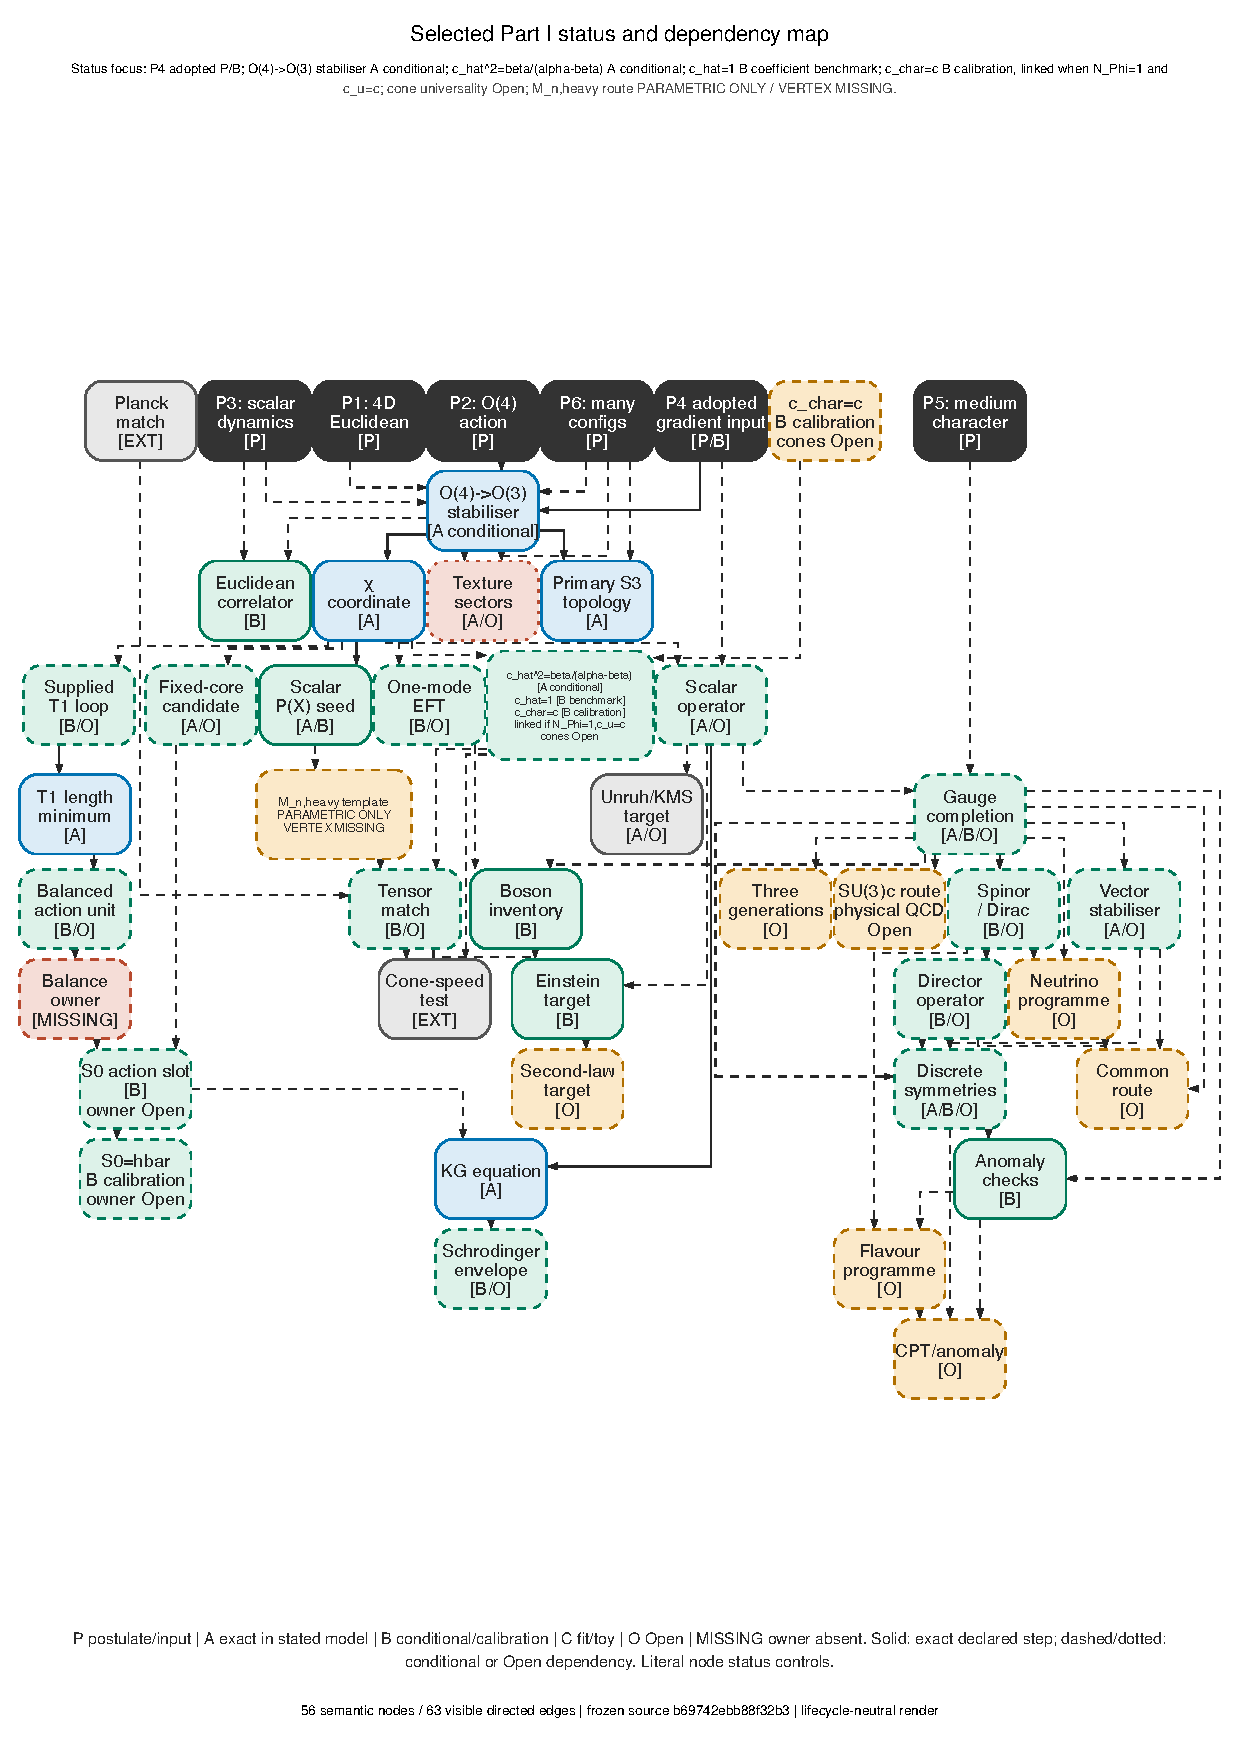
\includepdf[
  pages=1,
  pagecommand={\thispagestyle{empty}\phantomsection
    \refstepcounter{figure}
    \label{fig:partI_derivation_logic}
    \label{app:r141_complete_part_i_logic}
    \label{app:r129_visual_part_i_logic}
    \label{appfig:r123_atlas_fig09}
    \label{appfig:r123_topology_fig09}
    \addcontentsline{lof}{figure}{\protect\numberline{\thefigure}Selected status and dependency map of Part~I}}
]{figures/r185/logic_maps/partI_status_dependency.pdf}

\paragraph{How to read Figure~\ref{fig:partI_derivation_logic}.}
Starting from P1--P6, DP and the supplied coherent-branch closure~BR1, P4
supplies a preferred direction datum but does not fix the kinetic signs.  A
separately supplied $\alpha>\beta>0$ selects the retained Lorentzian scalar-PDE regime,
while clock, photon, matter and tensor matching remain separate.  The
compact-phase closure supplies winding sectors; the fixed-core and
tension-balanced action-scale candidates remain distinct from the
operational~$S_0$.  CDE-$\Phi$ and the texture-worldline reduction specify
an acceptance criterion and a generic route for what the actual 4D
action/state/profile/quotient owner would have to calculate, but the carrier,
compact modulus, stability and owner map are Open.  Gauge, charge, chirality and fermion
completion likewise retain their stated owners.  In particular, the allowed
homogeneous timelike vector-current operator is spin independent and supplies
no source-generated composition force; any spin or E\"otv\"os signal belongs to
a separately declared completion.

The calm colourblind-safe palette uses blue for results exact in their
declared model and assumptions, green for conditional constructions, pale
orange for fits or benchmarks, orange dashed borders for Open routes, neutral
gray for external inputs and charcoal for structural inputs.  These roles
remain distinguishable in grayscale through luminance, border/arrow form and
direct status labels; no hatch texture is required.  The vector poster is the
reader-facing topology authority.  Exact node/edge records and source hashes
remain in the repository machine-topology package rather than as a printed
multi-page edge ledger.

\paragraph{Foundational outcome of Part~I.}
Part~I establishes the minimal ECT core: an $O(4)$-invariant scalar medium,
a supplied gradient-ordered broken phase, a two-branch architecture, and a
layered low-energy sector decomposition.  Within the supplied P4/coefficient
EFT it classifies the scalar principal tensor.  Compact-phase winding and the
$\mathfrak{so}(3)\simeq\mathfrak{su}(2)$ algebraic correspondence are exact
only in their declared domains.  A physical clock and metric, local gauge
bundles and actions, an unbroken photon, chiral $SU(2)_L$ representations,
charges and matter assignments remain Open completion owners.  The coherent
branch rule~BR1 supplies conditional action-scale logic, and the
preferred-direction matter operator is distinct from the later scalar ansatz
S.  Other main open fronts include the microphysical origin of the gradient
condensate, nonlinear gravity, physical colour and fermionic completion,
matching of the scalar-background ansatz, and the separate map from S to the
conditional HRC gravity functional G.

The four cross-sector universalities isolated later in this chapter
(Section~\ref{par:four_universalities}) should be read as the capstone
compression of this foundational logic.

\subsection{Core axiomatic framework (Sections~\ref{sec:postulates}--\ref{sec:branching})}

The foundational layer of ECT establishes:
\begin{enumerate}
  \item A connected four-dimensional Euclidean arena with initially
    equivalent directions and points~(P1; ontology layer S1--S3).
  \item $O(4)$-invariant scalar microdynamics with the minimal
    variational realisation of the $\Phi$-medium~(P2--P3, DP).
  \item A supplied nonzero-gradient chart whose vector datum has $O(3)$
    stabiliser and defines the orientation variable~$n_A$~(P4);
    a stationary physical vacuum and spontaneous selection remain Open.
  \item The unique kinetic tensor
    $K^{AB}=\beta\,\delta^{AB}-\alpha\,n^A n^B$ of the broken
    phase~(Level~A; Theorem~\ref{thm:tensor_uniqueness}).
  \item Lorentzian signature as an ordered-branch admissibility condition:
    the broken-phase kinetic tensor
    $K^{AB}=\beta\,\delta^{AB}-\alpha\,n^A n^B$
    admits Euclidean, degenerate, and Lorentzian regimes.  It is hyperbolic
    exactly when $\beta(\beta-\alpha)<0$; on the retained healthy component
    this is $\alpha>\beta>0$ (Level~A conditional tensor algebra).
    This is not an observational selection rule and not an added
    postulate, but a mathematical admissibility property of the
    ordered-branch EFT.
  \item A two-step cone determination:
    first, independently supplied coefficients satisfying
    $\beta(\beta-\alpha)<0$ classify the scalar principal tensor as
    hyperbolic and give one scalar
    characteristic cone (Level~A mathematics in that EFT); it does not select
    the realised physical branch or a clock map.  Second,
    $\hat c_*^2=\beta/(\alpha-\beta)$ and the Level-B unit-slope coefficient
    benchmark $\hat c_*=1$ give $\alpha=2\beta$ inside that EFT.  The
    physical relations to clocks, photons, matter and tensor cones remain
    separate Open matchings.
  \item A scale-and-cone research architecture:
    the supplied scalar principal tensor fixes a common-length slope
    $\hat c_*$ (Level~A in that EFT), while physical $c_{\rm char}$ requires
    clock matching.  A future stationary P4 completion could test a heavy-pole
    matching ansatz $\kappa_n\sim u_0^2/m_{\rm P4,pole}^2$; neither that pole
    nor its vertex is presently derived.  The further
    $\kappa_n\to M_G^2$ remains an Open tensor bridge.  Independently,
    $\phi_0=\zeta_\phi\bar M_{\rm Pl}$, $\zeta_\phi>0$ and
    $\zeta_\phi=O(1)$, is the adopted Level-B scale ansatz; its microscopic
    explanation remains Open.  The coherent branch
    supplies two distinct loop-scale candidates and later conditional
    quantum closures reuse an operational action-unit slot $S_0$.  The
    owner map, nonzero universal value and cross-sector universality remain
    Open, while the physical identification $S_0=\hbar$ is Level~B matching
    (Sections~\ref{sec:cone_inheritance}, \ref{sec:three_scales},
    \ref{sec:hbar_status}).
  \item A layered arrow-of-time architecture with six nested
    levels~(A1--A6).  Retarded response and positive pairwise noise are
    retained; an ECT thermodynamic second law is Open because ohmicity and
    Markovianity alone are insufficient~(Section~\ref{sec:arrow_of_time}).
  \item Clear sector separation: homogeneous P3 amplitude curvature,
    Open P4 amplitude-pole programme, and the strict soft-orientation
    coordinate~$\chi$ reduced by integrability
    to one longitudinal scalar coordinate, and the macroscopic
    $\phi$-sector~(Section~\ref{sec:sector_map}).
  \item A hierarchy programme in which the primary microscopic amplitude
    $\phi_0$, a possible P4 pole, the orientation stiffness and the
    coherent action-scale programme are separate matching owners.  Their
    common microscopic descent and physical gravitational normalisation
    remain Open.
    The present open problem is no longer ``why are gravity and
    electroweak physics unrelated scales?'', but rather how one
    condensate generates a secondary low-energy matching scale
    $v_2\ll\phi_0$ while retaining the same medium origin
    (Section~\ref{sec:three_scales}).
  \item The coherent branch~BR1 with compact phase $\theta$,
    integer winding sectors, fixed-core representative
    $\iota_{\rm elem}^{\rm(fixed\ core)}=2\pi \iota_0^{\rm EFT}$ in the supplied
    reduced closure, together with
    the programme of testing whether one common action scale consistently
    normalises amplitudes, wave dynamics and canonical structure.  Born
    weights require an independently admitted probability measure and are
    not fixed by $S_0$.
  \item The supplied real-scalar action, together with its declared
    symmetries and DP, has conserved translational and rotational Noether
    currents.  Their Lorentzian energy--momentum reading is a separate ordered-
    branch interpretation; it does not supply the later EFT actions
    (Section~\ref{sec:noether}).
  \item A two-branch structure --- geometric macroscopic branch and
    coherent branch --- organised as candidate programmes of the same ordered
    medium.  P4 supplies the geometric chart and BR1 separately supplies the
    coherent closure; their common microscopic descent, back-reaction and
    equality of characteristic cones remain architectural hypotheses
    (Section~\ref{sec:branching}).
  \item Admissibility of non-uniform ordered
    backgrounds~(P6), treated here as an auxiliary structural
    admissibility assumption rather than a core dynamical postulate.
    Its r\^ole is to make branch-dependent inhomogeneous ordered
    configurations conceptually available for the later macroscopic
    $\phi$-sector development, not to derive that sector by itself.
\end{enumerate}

\paragraph{Capstone of the foundational layer.}
Taken together, these results organise a one-medium research architecture,
not a completed descent theorem.  The supplied scalar branch conditionally
fixes one scalar principal cone while physical clocks and cross-sector cones
remain Open; $(\phi_0,v_2)$ is kept distinct from the conditional HRC matching
length; and the coherent branch organises an action-scale programme.  The
macroscopic and quantum sections then introduce separately owned effective
actions, states, and observable maps.  Connecting those owners back to the
fundamental Euclidean action is an explicit Open programme, so later sections
must be read as conditional completions rather than automatic consequences of
one variational backbone.

\subsection{Gauge-sector architecture, particles, and fermions
(Sections~\ref{sec:gauge_and_fifth}--\ref{sec:fermions})}

Building on the core framework, the sector-development chapters
establish:
\begin{enumerate}[resume]
  \item The $U(1)$ phase--gauge correspondence: within the compact
    phase EFT, the Noether current and current conservation follow; after a
    local bundle/director are supplied, the two-invariant kinetic basis follows
    at Level~A/B with clearly stated
    assumptions~(Section~\ref{sec:u1_emergence}).
    This is the strongest gauge-sector result of Part~I.
  \item Structural embedding of non-Abelian gauge sectors:
    $\mathfrak{so}(3)\cong\mathfrak{su}(2)$ provides the cleanest
    algebraic bridge~(Level~A). For $SU(3)$, dimension excludes only a
    direct injective Lie-subalgebra/residual-factor embedding in the
    displayed minimal algebra~(Level~A conditional); P7 supplies the
    adopted positive-definite Hermitian rank-three bundle (Level-B), whose
    $SU(3)$ frame reduction is exact conditional mathematics.  Compact winding
    and the restricted Lie-algebra no-go are exact under
    their assumptions; local Abelian/chiral-$SU(2)$ sectors, alternative
    emergent/nonlinear, reducible/singlet, independent-bundle and
    defect-kernel colour routes, and physical colour remain Open
    (Sections~\ref{sec:nonabelian_embedding}--\ref{sec:ew_embedding};
    see also Section~\ref{sec:common_origin}).
  \item A three-category particle and excitation spectrum:
    (i)~kinematically identified or conditionally modelled condensate
    excitations ($\chi$, $\sigma$), with the physical $\chi$ mass and mode
    projector Open, and a physical graviton only as an Open completion target;
    (ii)~structurally embedded SM fields;
    (iii)~topological and conditional
    sectors~(Section~\ref{sec:particle_summary}).
  \item A conditional free-spinor reconstruction: the
    $\mathrm{Spin}(4)\to\mathrm{Spin}(3)$ representation bookkeeping and a
    Dirac-form low-energy operator can be written once the corresponding
    spinor completion is supplied.  This does not identify the physical
    fermion multiplets, a chiral weak bundle, its representations, or the
    Yukawa sector.  In particular, the vector order-parameter stabiliser is
    $SU(2)_{\rm diag}$ and selects neither $SU(2)_L$ nor $SU(2)_R$; the
    physical origin of weak chirality therefore remains Open
    (Section~\ref{sec:fermions}).
  \item The standard compact-$SU(2)$ origin of discrete spin projections,
    together with a conditional ECT route to its relevance: the supplied
    $O(4)\to O(3)$ vector chart has connected stabiliser $SO(3)$, whose
    spinorial double cover is $\mathrm{Spin}(3)\simeq SU(2)$
    (Level-A conditional group theory).  Identifying this stabiliser with the
    physical spatial-rotation group, and realising spinorial excitations on a
    physical three-dimensional slice, require separately supplied branch,
    metric/tetrad, spin-structure and matter-sector owners and remain Open.
    Conditional on a declared spin--apparatus--environment channel,
    Stern--Gerlach-type record formation may be analysed through the
    environmental-locking logic used elsewhere.  This supplies neither
    selection of one realised outcome nor its update rule; both remain Open.
  \item The ECT-specific fermion--condensate coupling
    $\Delta\mathcal{L}_5=\mu_5\,\bar\Psi\gamma^A n_A\Psi$:
    a candidate preferred-medium matter-sector deformation
    (operator inventory A-math conditional; coefficient, species law and
    physical map Open;~Section~\ref{sec:fifth_coupling}).
  \item Three-layer status separation: the microscopic $n_A$ operator M
    is not the Level-B scalar ansatz S, while the map from S to the supplied
    conditional HRC gravity functional G is Open
    (Section~\ref{sec:fifth_strength_range};
    Appendix~\ref{app:fifth_micro_macro};
    Figure~\ref{fig:ordered_branch_two_sectors}).
  \item Observability conditions and falsification logic for the
    ECT-specific coupling: four classes of observable channels
    identified (spin-sensitive, composition-sensitive, propagation,
    environment-dependent), together with explicit conditions under
    which the present ECT closure could be
    refuted~(Section~\ref{sec:fifth_observability}).
    No precision predictions are available at this stage.
  \item Structural constraints on the coupling coefficient:
    neither the coefficient nor the suppression scale, species dependence,
    $v_2$ corrections or radiative stability is selected by the present
    action~(Section~\ref{sec:fifth_coefficient_constraints}).
  \item A neutrino sector via type-I seesaw embedding with two
    independently supplied mass operators and scales.  The action derives no
    heavy scale, Yukawa, mixing or leptogenesis consequence
    (Section~\ref{sec:neutrino_particles}).
\end{enumerate}

\subsection{Status-separated structural statements and forward completion tests}

Part~I contains exact conditional statements, structural routes, external
gates, and Open completion tests.  None receives a common prediction status;
each is classified here by its own derivation level and owner.

\paragraph{Conditional homotopy classification of the supplied orientation target.}
The supplied target $O(4)/O(3)\simeq S^3$ has vanishing lower homotopy groups:
$\pi_0(S^3)=\pi_1(S^3)=\pi_2(S^3)=0$.
This is Level-A mathematics conditional on the target.  It becomes a physical
wall/string/monopole statement only after the target is identified with the
complete physical vacuum/configuration space and a transition owner is
supplied; those steps remain Open (Section~\ref{sec:predicted_states}).

\paragraph{Texture/skyrmion target classes (A-math conditional; physical Open).}
The non-trivial $\pi_3(S^3)=\mathbb{Z}$ guarantees integer classes of maps
into the supplied target.  In the separately supplied positive
two-derivative $S^3$ sigma model, $E_2(R)\propto R$ and Derrick collapse
follows.  Admissible exact-gradient ECT configurations, stabilising action,
profile, mass spectrum and production remain Open
(Section~\ref{sec:predicted_states}).

\paragraph{Ordered-branch signature classification and the supplied
second-order scalar cone (Level~A conditional / B physical).}
Part~I fixes the signature logic of the ordered branch in three distinct
steps.  First, on the full real coefficient plane the exact Level-A
classification inside the supplied scalar EFT is hyperbolic iff
$\beta(\beta-\alpha)<0$, elliptic iff the product is positive, and
degenerate for $\beta=0$ or $\alpha=\beta$.  The hyperbolic set has two
mathematical components: $\beta>0,\alpha>\beta$ and
$\beta<0,\alpha<\beta$.  Second, the separately supplied healthy
transverse-kinetic convention retains the first component, hence
$\alpha>\beta>0$; P4 does not select it.  Third,
$\hat c_*^2=\beta/(\alpha-\beta)$ and the adopted Level-B unit-slope
coefficient benchmark $\hat c_*=1$ give $\alpha=2\beta$ inside that supplied
branch; a common field rescaling cannot select this ratio.  The
the separate equality $c_{\rm char}=c$ is the adopted Level-B
scalar-clock calibration after fixing the conversion/lapse convention; a
microscopic explanation of that calibration and equality with photon and
tensor cones remain Open.  This reconstructed chain is a central non-circular
output of Part~I and stays conceptually separate from later decoherence- or
PES-based arguments.

\paragraph{Lorentz-invariance violation: missing physical operators
(Open).}
Part~I supplies no photon, neutrino or tensor LIV operator, coefficient,
common suppression scale or observable map.  External propagation data
constrain future named completions; no unit-coefficient benchmark or
cross-sector unification is retained
(Section~\ref{sec:effective_metric}).

\paragraph{Matching relations for emergent fundamental constants
(Level~A/B).}
Part~I collects separate candidate matching relations for the effective
propagation scale, gravitational normalisation, and coherent action
coefficient.  Their common one-medium origin is a matching programme, not a
derived common control by one parameter set.
At the ordered-branch level one has the separate conditional relations
\begin{align}
  \hat c_*^2 &= \frac{\beta}{\alpha-\beta}\,,
  \qquad
  G_N^{\rm nat} = \frac{1}{8\pi M_G^2}\,,
  \qquad
  \iota_0^{\rm EFT} = \frac{c_\perp\,K_\theta}{2\,m_\varphi^{2}}\,,
  \qquad
  \iota_{0,\rm bal}^{\rm eff}=\sqrt{2K_\theta^{1\mathrm D}\mathcal T_{\rm loop}}\,.
  \notag
\end{align}
The first relation is the dimensionless scalar slope at the EFT level;
$c_{\rm char}=c_{\rm u}\hat c_*/\mathcal N_\Phi$ requires the separate
clock map.
The second is the geometric matching relation that defines the effective
gravitational scale $M_G$ of the ordered branch; the explicit
microscopic relation between $M_G$ and the condensate parameters
remains an open derivational target.
The third and fourth are distinct coherent-sector loop-scale
candidates.  Mapping either one to the operational $S_0$ remains Open; the
subsequent $S_0=\hbar$ calibration is an adopted Level~B physical input rather
than a derivation.  Likewise $c_{\rm char}=c$ is the adopted Level-B
scalar-clock calibration; its microscopic explanation and cross-sector cone
universality remain Open.  These are independent matching inputs/programmes
and do not yet reduce the number of physical inputs.

\paragraph{Species dependence remains Open.}
The operator alone assigns no species law.  A multi-species signal requires
an explicit flavour-dependent matching and observable reduction
(Sections~\ref{sec:fifth_coupling} and
\ref{sec:fifth_observability}).

\paragraph{Longitudinal soft coordinate and conditional scalar mode.}
The integrability constraint reduces the naive three-component
Goldstone-coordinate map to one longitudinal scalar coordinate $\chi$ (Level~A
kinematics).  A supplied reduced EFT may realise one physical soft mode
(Level~B), but its existence, mass, stability and cosmological role are Open.
It is therefore only a possible dark-sector candidate, not a completed
dark-sector prediction~(Section~\ref{sec:particle_soft_orientation}).

\paragraph{Neutrino mass operators and scales (C/Open).}
The present ECT action selects no heavy-neutrino scale, Weinberg coefficient
or Yukawa matrix.  Consequently no ECT-selected numerical mass comparison,
Yukawa determination, active--sterile mixing, or leptogenesis inference
follows.  Fully declared unit-coefficient orientation points and inverse fits
remain admissible Level-C benchmarks, not predictions.  The theory does not
determine the absolute mass scale, the mass ordering, the PMNS pattern, or the
Dirac/Majorana character~(Section~\ref{sec:neutrino_particles}).

\paragraph{Conceptual outputs of Part~I.}
Beyond the formal structural results, Part~I produces the following
conceptual outputs that distinguish ECT from standard approaches:
(i)~\emph{Three logical classes of excitations:} ECT does not place
all candidate particle sectors on the same footing---condensate coordinates
and conditional modes,
structurally embedded SM fields, and topologically selected sectors
occupy different logical tiers, unlike QFT where all fields are
equally fundamental postulates~(\S\ref{sec:particle_structure}).
(ii)~\emph{Correlation versus interaction:} a common medium permits
product, classically correlated or entangled states; it does not by itself
derive a physical interaction, factorisation or exchange vertex.  Decoherence
does not create Lorentzian interactions.
(iii)~\emph{Open chiral completion:} the exact
$Spin(4)\simeq SU(2)_L\times SU(2)_R$ decomposition survives, but fixing the
ordered vector leaves $SU(2)_{\rm diag}$ and selects neither weak factor.
Physical chirality, CAR/spinor states and the weak vertex remain Open.
(iv)~\emph{Multi-excitation structure as a reconstruction target:}
ECT does not require Fock space as a foundational postulate; variable
particle number should emerge as a sector decomposition of one
condensate medium~(OP-Q11).
(v)~\emph{Conditional $3\!+\!1$ bookkeeping:} after P1 supplies four
Euclidean dimensions and P4 supplies one ordered direction, three transverse
coordinates remain.  This does not derive $D=4$, the ordered branch, a
physical clock, or why Nature has $3+1$ spacetime dimensions.
(vi)~\emph{Tensor completion:} at fixed $\alpha,\beta$ and tangent-director linear order about homogeneous $n=w$, the fixed director map has $h_{ij}^{\rm TT}=h_{ww}=0$.  The scoped theorem does not exclude quadratic/nonlinear/composite routes; a massless Fierz--Pauli sector is retained only as a conditional external completion target (Open).


\subsection{What Part~I derives and what it does not}

\paragraph{Exact or conditional mathematics retained.}
For supplied P4 and coefficients, the scalar principal tensor has the stated
form/sign classification and one scalar characteristic cone; the
integrability reduction is scoped in
\S\ref{sec:goldstone_integrability_main}.  The named scalar
initial-boundary problem admits the retarded solution of
Appendix~\ref{app:causal_hyperbolic}.  Standard
Euler--Lagrange/Noether identities, $\mathfrak{so}(3)\cong
\mathfrak{su}(2)$, and integer winding after supplied BR1 also survive in
their declared domains.  None of these derives a physical light speed,
universal matter/photon/tensor cone, metric, branch actualisation, gauge
sector, common gravity/quantum origin, or quantum action scale from P1--P3.

\paragraph{Conditional closures, matchings and Open bridges.}
$G_N$, $S_0=\hbar$ and $c_{\rm char}=c$ are comparison/matching inputs, not
derived constants.  Schr\"odinger, Einstein, local $U(1)$, Dirac, entropy
and spin-label constructions reproduce standard forms only after their
respective fields, states, operators, boundary conditions, gauge reductions
or channel hypotheses are supplied.  The director coefficient/species law,
weak sector, BR1 origin, gravitational/electroweak hierarchy and HRC gravity
bridge remain Open or Level-C benchmarks.

\paragraph{Supplied gauge/matter modules (conditional/Open).}
A compact phase gives global Noether algebra; bundle covariance is standard
mathematics only after a local $U(1)$ bundle is supplied.  The spacetime
orientation triplet is not an internal gauge field, and the vector stabiliser
selects no chiral factor.  Physical Abelian/weak/colour gauge fields,
couplings, representations, charges, anomaly cancellation, fermion masses,
Yukawa/flavour data and three generations remain supplied/Open rather than
derived from the minimal scalar.

\paragraph{Explicitly open.}
The dynamical origin of the gradient condensate~(OP-grad),
the energy-hierarchy mechanism and separate galactic matching~(OP-EW, OP-galactic),
the full graviton sector~(OP1), the full SM gauge completion
including colour derivation, matter representations, and anomaly
cancellation (OP-GUT1, OP-GUT2, OP-GUT3b, OP-GUT6 family in
Table~\ref{tab:op_gut}),
the full fermionic sector from first
principles~(Section~\ref{sec:fermion_open}),
the microscopic derivation of the fifth-coupling
coefficient, radiative stability of $\beta_5$, the full
quantum reconstruction from $S_0$~(Section~\ref{sec:quantum}),
and the microscopic H-theorem.

\subsection{What remains open at the end of Part~I}

The following list reformulates the open points above as concrete
research targets for Parts~II--III and for future work, rather than
repeating the derived/open classification itself.
The key open problems are:
\begin{itemize}
  \item Gradient condensate from bare action: the dynamical mechanism
    generating $\langle\partial_A\Phi\rangle\neq 0$ from
    P3~(OP-grad).
  \item Energy hierarchy: mechanism generating $v_2\ll\phi_0$
    (OP-EW); separately, derivation of the HRC matching length, $a_M$, and
    scalar-to-HRC gravity bridge~(OP-galactic).
  \item \textbf{OP-Planck:} Derive the full NLO
    orientation-stiffness coefficient $\mathcal{C}_n$ from
    first principles, including the induced contribution from
    integrating out the radial sector, the explicit map
    $\kappa_n\to M_G^2$ through the spin-2 normalisation,
    and a complete dimension-and-normalisation audit
    (Appendix~\ref{app:dim_audit}).
  \item Full derivation of the graviton sector: Fierz--Pauli closure,
    nonperturbative spectrum, gauge reduction~(OP1).
  \item Gauge/matter derivation: local $U(1)$ and chiral $SU(2)_L$
    are not selected by the global phase/vector stabiliser, and the
    $SU(3)_c$ module is supplied.  Derive the bundles, gauge-volume
    reduction, kinetic terms, representations, charges, anomaly
    cancellation and couplings (OP-GUT1, OP-GUT2, OP-GUT3b,
    OP-GUT6 family; see also
    Sections~\ref{sec:common_origin}
    and~\ref{sec:anomaly_architecture}).
  \item Full first-principles fermionic sector: dynamical origin of
    spinorial excitations, chiral gauge selection, Yukawa hierarchy,
    neutrino-mass mechanism, three
    generations~(Section~\ref{sec:fermion_open}).
  \item Microscopic derivation of the fifth-coupling coefficient
    $\mu_5$ from condensate microdynamics, and establishment of
    radiative stability.
  \item Derivation of an unbroken physical $U(1)_{\rm em}$, its
    transverse photon state, positive reduced Hessian, matter vertex and
    physical metric~(OP-gauge); only then can the Open relation
    $c_\gamma=c_{\rm char}$ be tested.  The scalar equality
    $c_{\rm char}=c$ is already the adopted clock calibration.
  \item Full mapping of the ECT-specific operator onto standard
    Lorentz-violation and equivalence-principle test frameworks.
  \item Full quantum reconstruction from $S_0$: amplitude composition,
    Born rule, operator algebra, Hilbert-space
    structure~(Section~\ref{sec:quantum}).
  \item Microscopic H-theorem: first-principles derivation of the
    decoherence kernel and irreversible thermodynamics.
  \item Nonlinear closure of each effective branch.
  \item Strict identification $\Sigma_\theta\,\iota_0^{\rm EFT}=\hbar$ beyond Level~B
    matching.
  \item Full subsystem-level reconstruction of quantum dynamics from the
    descriptive Euclidean condensate equation: in particular, the bridge
    from the deterministic boundary-value formulation of the coherent
    sector to the standard probabilistic subsystem equations beyond the
    presently established Schr\"odinger/Klein--Gordon reconstruction.
\end{itemize}

Additional open consistency problems of the emergent matter sector
are now organised explicitly in the structured OP-GUT family
(Table~\ref{tab:op_gut}) and the fermionic-architecture open
programme (\S\ref{sec:fermion_open}), including the conditional
CPT closure problem (OP-CPT1), the anomaly-consistency family
(OP-GUT6a, OP-GUT6b, OP-GUT6c), and the exact weak-sector parity
pattern (OP-P1).

\subsection{Roadmap to Parts~II--III}

{\small
\begin{longtable}{@{}L{3.5cm}L{5.5cm}L{5.5cm}@{}}
\caption{Structural branching of ECT after the foundational
construction.}
\label{tab:ect_branching}\\
\toprule
\textbf{Branch} & \textbf{Primary variables} & \textbf{Developed in} \\
\midrule
\endfirsthead
\toprule
\textbf{Branch} & \textbf{Primary variables} & \textbf{Developed in} \\
\midrule
\endhead
\bottomrule
\endfoot
Geometric (Macroscopic Physics)
  & $g^{\rm eff}_{AB}$, $n_A$, $\phi(X)$, and long-wavelength
    background variations of the ordered branch
  & Gravity, cosmology, galactic phenomenology,
    observational tests \\
Coherent (Quantum Sector)
  & $\Phi_{\rm eff}$, $\theta$, $S_0$, coherent winding sectors,
    and coherent correlators
  & Action-scale quantisation, wave dynamics,
    quantum kinematics, decoherence, probability \\
\bottomrule
\end{longtable}
}

\noindent
\textit{Part~II} (Section~\ref{sec:macroscopic} onwards) develops
the geometric macroscopic branch: the homogeneous ordered-phase limit,
the emergent gravitational sector, the ordered-branch cosmological
programme, galactic and cluster-scale phenomenology, dark-sector
interpretation, and observational tests.
Part~II distinguishes a Level-B scalar ansatz from separately supplied conditional HRC galactic phenomenology.  Part~I establishes only that the
microscopic $n_A$ operator is a different object; it does not supply the
Open scalar-to-AQUAL source/force map
(Section~\ref{sec:fifth_to_galactic_bridge}).

\noindent
\textit{Part~III} (Section~\ref{sec:quantum} onwards) develops
the phase-sensitive coherent branch across eleven thematic steps:
coherent phase dynamics and the pre-quantum action scale, wave
kinematics and conservation laws, the Hilbert-space bridge
(reflection positivity, unitarity, canonical structure, uncertainty),
exchange sectors and Dirac structure, unified vacuum response,
decoherence and the arrow of time, the quantum--classical boundary and
Born-type probability, entanglement, the wider topological/dark-sector
ontology, black-hole thermodynamics and the information problem, and
the analogue-laboratory programme.


% ============================================================
% LABEL ALIASES for backward compatibility
\label{sec:gravity}%           was: \section{Gravitational Sector}
\label{sec:lorentz_order_field}%was: \section{The Lorentz-Order Field}
\label{sec:galactic}%           was: rotation-curve section
\label{sec:cosmology}%          was: \section{Cosmological Implications}
\label{sec:phi_first_strategy}% was: phi-first strategy subsection
% ============================================================

\FloatBarrier
%==============================================================
\clearpage
\part{Macroscopic Physics: Gravity, Cosmology, and Observational Tests}
\label{part:macro}
%==============================================================

% ============================================================
% MACROSCOPIC PHYSICS — ECT
% File: mp.tex
% Version: 10  (2026-03-16, pre-integration final)
%
% VERSION HISTORY:
%   v4:  §6.2 fully replaced — fixed metric formula g_eff^{AB}=β·δ-α·n·n;
%        Level A/B status split for metric vs φ-first closure
%   v5:  §6.3 FP-like wording; §6.4 schematic EMT_n; §6.5 derivation chain;
%        §6.6 Bianchi eq, homogeneous limit fix, neighbour-theory comparison
%        §6.9 pre-Lorentzian scenario, V(Φ) inflaton language corrected;
%        §6.10 HRC scale diagnostics; §6.11 schematic lensing, exploratory BH;
%        §6.12 table updates (Pre-Lorentzian Level B, baryogenesis route)
%   v7:  FLRW Lambda_eff dimensional fix; r removed from §6.8 → §6.9;
%        §6.7 PPN estimate corrected and citations added
%        (Bertotti2003, Uzan2011, Planck2018, DESI2024, Cromartie2020,
%        Riley2021, Lelli2016, McGaugh2016)
%   v8:  All 9 figures inserted with updated captions (timeline, cosmo,
%        w_z, sparc, MW, EFE, rar, hrc_scale, bullet_cluster)
%   v9:  §6.10 tab:phi_fits (6 galaxies), baryonic modelling, caveats
%        subsection added; figures/ paths verified
%   v10: Header updated for integration; all 4 deferred-basics sections
%        confirmed covered (sec:geom_branch, sec:noether, sec:spin2_content,
%        sec:GN_matching); pre-integration verification passed 15/15
%
% DISCIPLINE:
% (1) Every claim: Level A / B / EFT / matching / phenomenological / open.
% (2) Two parallel lines: mathematical + physical.
% (3) No import of hbar, Born rule, full QM.
% (4) Deferred basics subsections DEVELOPED here.
% (5) Old content preserved, improved, not shrunk.
% (6) Every strong claim \ref{} or \cite{}.
% (7) Comparisons with GR/BD/Einstein-aether preserved.
% (8) Numerical estimates tracked with status.
%
% ============================================================
% (1) Every claim: Level A / B / EFT / matching / phenomenological / open.
% (2) Two parallel lines: mathematical + physical.
% (3) No import of hbar, Born rule, full QM.
% (4) Deferred basics subsections DEVELOPED here.
% (5) Old content preserved, improved, not shrunk.
% (6) Every strong claim \ref{} or \cite{}.
% (7) Comparisons with GR/BD/Einstein-aether preserved.
% (8) Numerical estimates tracked with status.
% ============================================================

\section{Scope, Bridge, and Approximation Hierarchy}
\label{sec:macroscopic}
\label{sec:mp_scope}

{\itshape
Part~II develops the macroscopic physics of the ordered
condensate branch.
Before proceeding to the specific derivations---local
special-relativistic kinematics~(\S\ref{sec:sr_limit}), the
gravitational sector~(\S\ref{sec:mp_gravity}), cosmology, and galactic
phenomenology---the present section fixes the scope, states the
approximation regime, and records explicitly which results of Part~I
are used as structural inputs below.

The purpose of this section is threefold.
First, to define the branch of the theory developed in Part~II.
Second, to make explicit which approximations are used, where they
enter, and what their derivation status is.
Third, to draw a sharp boundary between what Part~II imports from
Part~I and what it does not import from the Quantum Sector of Part~III.

Throughout this chapter we distinguish three levels of status:
strictly derived structural inputs from Part~I~(Level~A),
structural but conditional results inherited from controlled
reconstruction routes~(Level~B), and closure-dependent macroscopic
specialisations used in phenomenology.
}

% ============================================================
\subsection{Macroscopic Physics as the development
of the geometric branch}
\label{sec:mp_intro}
% ============================================================

\textit{Connection to ECT Foundations (Part~\ref{part:foundations}):
Sections~\ref{sec:branching}, \ref{sec:geom_branch},
and the summary rules collected in
Section~\ref{sec:foundational_consequences}, especially the
amplitude--orientation decomposition rule and the macroscopic
viability rule.
Status: conceptual bridge; all claims structural.}

\medskip
After completing ECT Foundations
(Sections~\ref{sec:postulates}--\ref{sec:branching}),
ECT is no longer an undifferentiated scheme.
As organised in the branching section, P4 supplies an ordered-gradient chart
and BR1 separately supplies a coherent-sector closure.  The manuscript then
studies phase-insensitive geometric and phase-sensitive coherent programmes;
no physical branch selection or common microscopic descent is derived.
The present section follows the first of these developments.
Throughout Part~II we work with the derived scalar cone and, wherever SI
units are displayed, use the adopted Level-B scalar-clock calibration
$c_{\rm char}=c$.  Part~I does not supply the reduced gauge bundle, unbroken
photon or physical photon principal operator required to establish the
separate equality $c_\gamma=c_{\rm char}$
(\S\ref{sec:cone_inheritance}).

\paragraph{Two conditional programmes organised around one medium.}
The manuscript organises a \emph{geometric/macroscopic programme}
(\S\ref{sec:geom_branch}) around phase-insensitive long-wavelength
variables and a \emph{coherent/quantum-reconstruction programme}
(\S\ref{sec:coh_branch}) around a separately supplied complex closure,
winding sectors, reduced-state kernels and amplitudes.  This organisation is
the one-medium architecture being tested; it is not a derivation that one
frozen scalar action already owns both physical sectors.  Each programme
requires its own action, state, constraint reduction and observable map.
The present section develops the first programme exclusively.
The Level-B scalar ansatz of Part~II is an amplitude/background closure
within this programme.  The supplied conditional HRC gravity functional is a separate
response construction whose connection to that ansatz remains Open; neither
should be confused with the coherent phase $\theta$.

\paragraph{Definition of macroscopic programme variables.}
ECT Foundations supplies an ordered-gradient chart and separately defines a
BR1 coherent closure.  The subsequent analysis is organised into a
\emph{tensorial, phase-insensitive programme} and a
\emph{coherent, phase-sensitive programme}; their physical common owner is Open.
The geometric branch is defined precisely by the former.
The primary variables and completion symbols of this programme are:
\begin{itemize}
  \item the scalar characteristic tensor $K^{AB}$ and its convenient
    inverse metric-like notation; a universal physical metric remains Open;
  \item the orientation collective variable $n_A$~(P4);
  \item long-wavelength orientation coordinates $\delta n_i$
    around the supplied chart~(Section~\ref{sec:goldstone_integrability_main});
  \item action-specific Noether stress and angular-current structures
    (Section~\ref{sec:noether}, Appendix~\ref{app:noether_full});
  \item the conditional tensor coefficient $M_G$ in a supplied gravity
    completion; the bridge from orientation stiffness to $M_G$ and then to
    the observed Newton constant is Open.
\end{itemize}
Some precursor symbols appear in ECT Foundations, but their physical metric,
tensor, source and matching ownership is not thereby established.

\paragraph{The conditional coarse-graining criterion.}
A macroscopic P4 programme may be organised only after a P4 pole is supplied.
Define conditionally
\begin{equation}
  \label{eq:macro_regime}
  L\gg\xi_{\rm P4}:=m_{\rm P4,pole}^{-1},
  \qquad E\ll m_{\rm P4,pole}.
\end{equation}
The P3 value $m_{\Phi,\mathrm{rad}}^2=2\mu^2$ does not own
$m_{\rm P4,pole}$.  Thus Eq.~\eqref{eq:macro_regime} is a conditional EFT
regime, not a derived numerical cutoff, until the stationary P4 action and
Hessian are supplied.  Coarse graining also does not prove the retained
orientation/background inventory to be complete.

\paragraph{Why the phase drops out.}
The macroscopic branch is defined not only by scale but by
the loss of sensitivity to local phase information.
In geometric-branch observables the phase $\theta$ of the
coherent order parameter $\Phi_{\rm eff}$ does not appear
explicitly; what remains are effective metric relations,
source couplings, causal propagation, and large-scale
background structure.
This is the bookkeeping reason why the present section studies conditional
gravity, cosmology and galactic completions, while wave amplitudes, operator
algebra, decoherence and probability owners are analysed separately.  It is
not a theorem that coarse graining alone produces either completed sector.

\paragraph{What is already established in ECT Foundations.}
From ECT Foundations the following conditional inventory is available for the
geometric programme: the supplied chart is parametrised by collective
infrared variables~(Section~\ref{sec:ordered_branch_eft}), and the declared
local algebraic scalar operator inventory fixes its two-tensor basis.  A
physical coarse-grained tensor owner remains Open.
\begin{enumerate}[label=(\roman*)]
  \item a constrained soft orientation sector (integrability gives one
    longitudinal scalar coordinate $\chi$ in the strict scalar map; its
    one-mode physical interpretation is a Level~B minimal-EFT statement;
    see Section~\ref{sec:goldstone_integrability_main}
    and Appendix~\ref{app:goldstone_integrability});
  \item conditional scalar Lorentzian component $\alpha>\beta>0$ once the
    healthy sign, P4 chart and EFT coefficients are supplied; the optional
    arithmetic-average benchmark $\alpha<4\beta$ requires its own declared
    ensemble/cell and is not a homogenised or physical viability bound
    (Section~\ref{sec:lorentz_window});
  \item action-specific conserved $T^{AB}$ from translational invariance
    and angular currents $J^{C,AB}$ from $O(4)$ invariance
    ~(Section~\ref{sec:noether}, Appendix~\ref{app:noether_full});
  \item a conditional tensor-normalisation symbol $M_G$ is introduced for
    a supplied gravity completion; its microscopic owner and the bridge from
    orientation stiffness are Open, while standard matching to $G_N$ is
    reviewed in Section~\ref{sec:mp_matching};
  \item a conditional Deser-type self-coupling route, applicable only after a healthy universal spin-2 seed and source vertex are independently derived~(Section~\ref{sec:mode_hierarchy});
  \item[(vi)] the scalar-cone result: integrability of
    $Q_A=\partial_A\Phi$ forces the linear scalar ordered branch into
    a single principal slope~$\hat c_*$ in common-length coordinates
    (Level~A inside the supplied scalar EFT); its physical speed requires
    $c_{\rm u}$ and $\mathcal N_\Phi$;
  \item[(vii)] restricted cross-sector cone programme: the scalar cone is
    derived, and the coherent-phase and Abelian-gauge routes share it under
    their stated matching assumptions.  The physical tensor principal
    symbol and $c_{\rm GW}$ remain Open
    (\S\ref{sec:cone_inheritance}, Eq.~\eqref{eq:cone_universality});
  \item[(viii)] the physical identification $c_{\rm char}=c$ is the
    adopted Level-B scalar-clock calibration; the photon and tensor cone
    equalities remain independent Open kill gates.
\end{enumerate}

\paragraph{Four structural common-origin programmes of ECT.}
\label{par:four_universalities}
The single-medium architecture~(P3) motivates four cross-sector
universality programmes with different closure status:
\begin{enumerate}[label=(\Roman*)]
  \item \textbf{Common-cone programme:}
  the scalar characteristic cone is derived; phase and Abelian-gauge
  inheritance is conditional on their stated maps, while the physical
  tensor cone is Open (\S\ref{par:cone_universality},
  Eq.~\eqref{eq:cone_universality}).
  \item \textbf{Common action-scale programme:}
  a common parameter~$S_0$ is used across supplied coherent-branch
  constructions.  Its universality and identification to $\hbar$ remain
  matching problems~(\S\ref{par:action_scale_universality}).
  \item \textbf{Common extremal-backbone programme:}
  stationary or variational principles occur in the declared bare and
  reduced models, but a universal one-history physical identity across
  macroscopic, open-system and quantum sectors is not derived
  (\S\ref{par:extremal_backbone}).
  \item \textbf{Common conservation-owner programme:}
  translational/$O(4)$ Noether currents of the real scalar action, the
  phase current and winding of the supplied BR1 closure, and the later
  probability-current reading are distinct structures.  A single reduced
  action/state owner connecting all of them remains Open
  (\S\ref{sec:qs_conservation}).
\end{enumerate}
These are conceptually distinct research programmes probing causal
propagation, action normalisation, variational organisation and conservation
structure.  They are not evidence that one medium already owns all their
operators, states or measured normalisations.  The observed single values of
$c$ and $\hbar$ are matching targets and cannot validate common microscopic
ownership before the corresponding bridges are derived.

\paragraph{Combined falsifiable content of the universalities.}
If \emph{any} of the four proposed common-origin links were shown to be
impossible---for example if completed native sectors required incompatible
causal cones, action scales or conservation owners---then the corresponding
ECT single-medium programme would fail.
Such an outcome would show that the native low-energy sectors of the
theory are not controlled by one and the same condensate structure.
Conversely, the present incompleteness of the bridges is not positive
evidence for common ownership.  Each link must be tested only after the
relevant physical actions, states and observable maps are supplied.

\paragraph{Programme-level failure-gate map.}
\label{par:falsifier_map}
The programme developed in Parts~I--III admits a compact status map in which
structural routes are paired with the conditions that would reject a
specified completion and with external observational constraints relevant
after that completion is supplied.  The current Open routes are not thereby
promoted to predictions or already-operational falsifiers.
Table~\ref{tab:falsifier_map} collects thirteen programme-level failure gates.

\begin{longtable}{@{}L{3.7cm}L{4.6cm}L{6.3cm}@{}}
\caption{Status-separated failure gates of the current ECT programme.}
\label{tab:falsifier_map}\\
\toprule
Programme statement & Failure condition for the named completion & External constraint or future test window \\
\midrule
\endfirsthead
\multicolumn{3}{l}{\textit{Table~\ref{tab:falsifier_map} continued}}\\
\toprule
Programme statement & Failure condition & External constraint / future window \\
\midrule
\endhead
\midrule
\multicolumn{3}{r}{\textit{Continued on next page}}\\
\endfoot
\bottomrule
\endlastfoot
Common-cone programme (\S\ref{par:cone_universality})
  & Sector-dependent limiting speeds
  & $|c_{\rm GW}/c-1|\lesssim10^{-15}$
    \cite{LIGO_Fermi_GW170817_GRB2017} \\
Common action-scale programme (\S\ref{par:action_scale_universality})
  & Mutually inconsistent quantum-sector normalisations
  & Single $\hbar$ across all established quantum phenomena \\
One extremal backbone (\S\ref{par:extremal_backbone})
  & Incompatible sector-dependent extremal/classical crossover
    criteria in native ECT sectors
  & Interferometric, atomic, and macroscopic regimes are all
    consistent with action-controlled crossover logic, while the
    precise universal threshold remains a structural programme-level
    claim rather than an established measured law \\
One conservation origin (\S\ref{sec:qs_conservation})
  & Independent non-condensate conservation structures
    for native sectors
  & Charge stability bounds such as
    $\tau(e\to\gamma\nu)>10^{26}\,$yr~\cite{ParticleDataGroup2022};
    the broader baryogenesis connection is developed separately in
    Section~\ref{sec:baryogenesis} \\
Candidate electroweak completion (separately supplied;
  \S\ref{sec:gauge})
  & No ECT-specific falsifier exists until a named local
    $SU(2)_L\times U(1)_Y$ bundle, action, chirality and matter
    representations are derived or supplied
  & Once supplied, test anomaly cancellation, charge assignments, the
    unbroken photon and the mass pattern; the observed Standard-Model
    organisation is an external target, not verification of an ECT route \\
Open entanglement-from-medium reconstruction programme
  (\S\ref{par:entanglement_programme})
  & After a physical state/channel is derived, no reconstruction from the
    medium is possible without importing the full tensor-product structure
    as an independent primitive
  & Bell-inequality violation well established;
    loophole-free tests confirm non-classical
    correlations \\
Tensor-closure graviton programme (\S\ref{par:tensor_falsifier})
  & Induced metric sector cannot close to FP/TT,
    or tensor cone differs from ordered branch
  & GW speed $|c_{\rm GW}/c-1|\lesssim10^{-15}$;
    no extra polarisations detected \\
Analogue source-model comparison programme (\S\ref{par:analogue_programme})
  & A frozen analogue--ECT bridge fails after its source action, state,
    operator, observable, uncertainty and discriminator guards pass
  & Quantised circulation, dynamical Casimir, acoustic mode mixing and
    tunable decoherence are external source-model results; they are neither
    evidence for ECT nor a generic ECT falsifier \\
Quantum-sector one-medium unification (\S\ref{par:quantum_programme})
  & Different quantum substructures requiring
    mutually unrelated action scales or principles
  & All established QM phenomena remain consistent with
    a single $\hbar$, one effective probabilistic layer of Born type,
    and one Schr\"odinger dynamics \\
Singularity as branch boundary (\S\ref{par:singularity_programme})
  & Ordered branch remains valid to formal GR
    singularity with no condensate breakdown
  & No observed sub-Planckian singular physics;
    BH exterior consistent with EFT description \\
P4 radial-mode EFT-threshold programme (\S\ref{par:uv_threshold})
  & A stationary P4 action fails to produce a healthy isolated amplitude
    pole, or its derived threshold conflicts with observation
  & No P4 pole or threshold is presently predicted; this row is a future
    theory-and-data gate, not a passed test \\
Einstein nonlinear closure (\S\ref{sec:mp_nonlinear})
  & Non-Einstein two-derivative completion required,
    or non-universal matter-metric coupling
  & Classical GR weak-field success; binary-pulsar
    radiative consistency; absence of compulsory extra
    low-energy tensor polarisations.
    External sensitivity footprint of $\mathcal X^{\rm cand}_{\mu\nu}[n]$
    inventoried across five sectors (Table~\ref{tab:nlee_footprint}); no ECT
    contribution is identified before $S_n$, projection, sign, and coefficients
    are derived~(OP-c1) \\
Galactic dark-sector fit scope (\S\ref{sec:mp_dark})
  & Failure of the HRC no-halo algebraic diagnostic on held-out galactic data
  & Level-C SPARC fits and conditional BTFR/RAR algebra use the matched
    $a_M$ benchmark; scalar-to-galactic matching and ECT particle
    content remain Open \\
\end{longtable}

\noindent
The same map yields conditional programme-level hypotheses:
\begin{enumerate}[label=(\roman*)]
  \item No native low-energy sector should require its own
  independent fundamental action unit: all coherent-branch
  normalisations should reduce to one operational~$S_0$, after an explicit
  owner map rather than by identifying either loop candidate by notation.
  \item No native low-energy sector should require its own
  independent extremality law: all effective equations of motion
  should descend from one dynamical principle~DP.
  \item Any future tensor completion must pass the external constraint
  $|c_{\rm GW}/c_\gamma-1|\lesssim10^{-15}$; the present scalar action
  predicts neither equality nor Planck-suppressed departures
  (\S\ref{sec:mp_gw}).
  \item If the ordered-medium electroweak route is correct, future
  deeper closure should \emph{reduce} external gauge input rather
  than increase it.
  \item Cosmological, decoherence, and vacuum-response developments
  should reinforce cross-sector unification rather than fragment
  into unrelated sector-specific constants.
\end{enumerate}
These are programme-level hypotheses: each is falsifiable in
principle but tests the overall architecture rather than a single
formula.
Their collective consistency forms a major part of the present
structural case for the ECT single-medium programme.

\paragraph{What does not follow automatically.}
Items~(i)--(viii) above do not automatically give:
the full nonlinear gravitational closure;
standard Einstein equations in final form;
complete matching of all phenomenological constants;
or any quantum-mechanical statement.
These are developed step by step below.

\paragraph{Logical order of Part~II.}
First: the homogeneous ordered-phase limit and emergent special
relativity~(\S\ref{sec:sr_limit}).
Then: the macroscopic gravitational sector, including the effective
metric, source structure, gravitational stiffness matching, nonlinear
closure, weak-field limit, post-Newtonian regime, and gravitational
waves~(\S\S\ref{sec:mp_metric}--\ref{sec:mp_gw}).
Finally: cosmology, galactic phenomenology, dark-sector
interpretation, and observational
tests~(\S\S\ref{sec:mp_cosmology}--\ref{sec:mp_tests}).
The conditional HRC gravity functional G used later is separately
supplied.  Its response algebra is Level~A inside the augmented model,
the map from the ordered phase or scalar ansatz S is Level~B/Open, and
its data applications are Level~C.

\paragraph{What Part~II does not import from Part~III.}
The macroscopic branch is constructed without using the reduced Planck constant
$\hbar$, the Born rule, wavefunction collapse, canonical commutation
relations, decoherence functionals, or instanton/loop amplitudes.
These belong exclusively to the Quantum Sector developed in Part~III.
The role of Part~II is purely geometric and macroscopic.
Accordingly, all macroscopic equations in Part~II are organised without
taking $\hbar$ as a dynamical input of the geometric branch itself.
In particular, the action-scale logic associated with $S_0$ and its
matching to $\hbar$ is not used as an input to the geometric branch,
even when $c$ and $G_N$ are already employed as matched macroscopic
constants.

\paragraph{Branch structure at the coarse-grained level.}
At the coarse-grained level relevant for the present chapter,
observables separate into a phase-insensitive geometric development and
a phase-sensitive coherent development.  Part~II develops
only the former.  This distinction is sufficient for the present scope
and does not require a stronger theorem-level claim of exhaustive RG
classification.

\paragraph{Physical picture.}
If ECT Foundations answers: \emph{what is the ordered medium and how
does it branch?}, then Macroscopic Physics answers:
\emph{how does the geometric branch of that medium appear to a
large-scale observer insensitive to coherent phase data?}
Gravity is not introduced as an independent external sector.
Rather, the working hypothesis of Macroscopic Physics is that the
large-scale causal and geometric response of the ordered condensate
admits an effective description which, in the viable Lorentzian
branch, takes geometric form.


% ============================================================
\subsection{Approximation hierarchy used in Part~II}
\label{sec:approx_hierarchy}
% ============================================================

The derivations of Part~II use a nested sequence of approximation
regimes.  The table below records the approximation levels explicitly
used in the chapter and indicates where each of them enters.
The purpose is organisational clarity rather than a theorem-level claim
of formal completeness.

\renewcommand{\arraystretch}{1.3}
{\small
\begingroup
\setlength{\tabcolsep}{5.69pt}
\begin{longtable}{@{}L{4.0cm}L{4.8cm}L{3.5cm}L{2.5cm}@{}}
\caption{Approximation levels used in Part~II.}
\label{tab:approx_hierarchy}\\
\hline\hline
Approximation & Validity condition & Where used & Origin / status \\
\hline
\endfirsthead
\hline\hline
Approximation (cont.) & Condition & Where used & Status \\
\hline
\endhead
\hline
\endfoot
\hline\hline
\endlastfoot
Conditional retained scalar hyperbolic component
  & $\beta>0$, $\alpha>\beta$
  & All of Part~II
  & Level~A mathematics inside the supplied scalar operators; physical
    macroscopic viability and a common metric remain Open
    (\S\ref{sec:lorentz_window}) \\
Optional arithmetic-average benchmark
  & $\alpha<4\beta$ only after a declared ensemble/cell, scale
    $\ell_{\rm iso}$ and arithmetic isotropic averaging prescription
  & Only where separately invoked
  & Conditional coefficient-average positivity; not a Lorentzian boundary,
    homogenised operator or derived ultraviolet window \\
Conditional P4 macroscopic EFT regime
  & $L\gg\xi_{\rm P4}$, $E\ll m_{\rm P4,pole}$
  & Only owner-declared P4-EFT formulae
  & Open until a stationary P4 Hessian, positive pole and scale separation
    are derived \\
Homogeneous supplied ordered chart
  & $\nabla n_A=0$, $\alpha,\beta=\mathrm{const}$
  & \S\ref{sec:sr_limit} (SR)
  & Level~A conditional kinematics; stationary physical phase and selection
    Open \\
Linear perturbative regime
  & $|\delta n_i|\ll 1$ (equivalently
    $|\partial_i\chi|/u_0\ll1$ in the declared linear map)
  & \S\ref{sec:mp_tensor} (linearised gravity)
  & Level~A conditional expansion; physical linearised-gravity owner Open \\
Minimal nonlinear closure
  & A1--A4, amplitude-dominated reduction
  & \S\ref{sec:mp_nonlinear} (generalised EE)
  & Level~B \\
Algebraic frozen-$F$ limit
  & $F=\mathrm{const}$ and scalar derivatives vanish; no independent
    orientation source included
  & \S\ref{sec:mp_ppn} (conditional GR reduction)
  & Level~A algebra inside the Level-B ansatz; dynamical reachability Open \\
Weak-field, quasi-static
  & $|h_{\mu\nu}|\ll 1$, $v\ll c_{\rm char}$, $|\partial_t|\ll c_{\rm char}|\nabla|$
  & \S\ref{sec:mp_newtonian} (Newtonian limit)
  & Level~B within the adopted closure \\
FRW background specialisation
  & $n_A\to\bar n_A$, $\phi=\phi(t)$, isotropic
  & \S\ref{sec:mp_cosmology} (cosmology)
  & Level~B background ansatz \\
Critical IR galactic regime
  & deep-acceleration branch with non-analytic IR closure
  & \S\ref{sec:mp_galactic} (galaxies)
  & Closure-dependent \\
\end{longtable}
\endgroup
}

These approximations should be understood as the explicit approximation
map used in the present chapter.  They are introduced here in order to
make the logical dependencies of the later derivations transparent.

% ============================================================
\subsection{Bridge from Part~I: structural inputs used in Part~II}
\label{sec:bridge_inputs}
% ============================================================

The list above states the conceptual content in prose; the table below
recasts the same inherited results as an operational bridge map for the
later macroscopic derivations.
The following table records the items retained from Part~I that are
used as structural inputs in Part~II.  It is intended as a bridge map:
for each inherited item, we indicate its status and
what role it plays in the macroscopic development.

\renewcommand{\arraystretch}{1.3}
{\small
\begin{longtable}{@{}L{4.8cm}L{1.6cm}L{2.1cm}L{5.9cm}@{}}
\caption{Structural inputs from Part~I used in Part~II.}
\label{tab:bridge_inputs}\\
\hline\hline
Part~I item & Level & Section & Role in Part~II \\
\hline
\endfirsthead
\hline\hline
Part~I item (cont.) & Level & Section & Role \\
\hline
\endhead
\hline
\endfoot
\hline\hline
\endlastfoot
P4-supplied nonzero vector $n_A$ with $O(3)$ stabiliser
  & Supplied datum / A-math; physical SSB Open & \S\ref{sec:ssb}
  & Conditional scalar orientation chart; no physical causal structure by
    itself \\
Unique $K^{AB}=\beta\delta^{AB}-\alpha n^A n^B$
  & A-math conditional & \S\ref{sec:tensor_uniqueness}
  & Supplied scalar operator basis; physical metric Open \\
Retained scalar Lorentzian component $\beta>0$, $\alpha>\beta$
  & A-math conditional / physical Open & \S\ref{sec:lorentz_window}
  & Exact scalar hyperbolicity on the supplied healthy component; the optional
    arithmetic-average condition is a separate assumption, not part of this row \\
Supplied second-order scalar operator: one principal cone
  & A-math conditional / B physical & \S\ref{sec:goldstone_integrability_main}
  & Integrability fixes the coordinate map, not operator order; no GW-speed owner \\
$\hat c_*^2=\beta/(\alpha-\beta)$
  & A-math conditional & \S\ref{sec:c_star}
  & Dimensionless scalar characteristic ratio on the retained component \\
$c_{\rm char}=c$ (scalar-clock calibration)
  & Level~B adopted & \S\ref{sec:cone_inheritance}
  & Uses a declared clock/lapse convention; microscopic owner Open, while
    photon/tensor cone equality requires separate actions \\

Ordered-branch collective variables
  & A-math/B/Open & \S\ref{sec:ordered_branch_eft}
  & Conditional amplitude/$\phi$ coordinates and orientation reduction;
    physical modes require their actions and projectors \\
On-shell Noether currents $T^{AB}$, $J^{C,AB}$
  & A-math in their owning actions & \S\ref{sec:noether}
  & Current identities only; no gravitational source vertex or Bianchi identity follows \\
Phase-to-gauge completion route (L1--L3)
  & Open & \S\ref{sec:gauge}
  & transverse photon and $c_\gamma=c_{\rm char}$ require independent owners \\
\end{longtable}
}

\paragraph{Immediate matching step in Part~II.}
In addition to the inherited inputs listed above, Part~II performs the
gravitational stiffness matching
\[
  G_N^{\rm nat} = \frac{1}{8\pi M_G^2},
\]
which is not an input from Part~I but an early macroscopic matching
step carried out within the present chapter~(\S\ref{sec:mp_matching}).

\paragraph{Characteristic scales of the macroscopic regime.}
Conditional on a stationary P4 action and pole, the geometric EFT may be
organised at
\[
 L\gg\xi_{\rm P4}=m_{\rm P4,pole}^{-1},
 \qquad E\ll m_{\rm P4,pole}.
\]
Neither quantity is inherited from the P3 homogeneous radial pole.  The
dimensionless scalar slope $\hat c_*$, the physical clock/photon speed and the
tensor normalisation $M_G$ likewise have distinct owners.  Therefore P3,
P4, photon and tensor scales must be matched rather than identified by
notation.


% ==============================================================
\section{Special Relativity as the Homogeneous Ordered-Phase Limit}
\label{sec:sr_limit}
% ==============================================================

Before allowing the ordered condensate background to vary across
spacetime, it is useful to isolate the homogeneous limit in which the
effective geometry is flat.  This limit provides the local
special-relativistic kinematics on which the subsequent macroscopic
gravitational construction is built.

The logic is the following.  Conditional on the supplied P4 ordered
branch, residual $O(3)$ covariance permits the displayed scalar kinetic tensor
$K^{AB}=\beta\,\delta^{AB}-\alpha\,n^A n^B$
(Theorem~\ref{thm:tensor_uniqueness}), while integrability of
$Q_A=\partial_A\Phi$ reduces the strict linear soft map to one scalar
coordinate~(\S\ref{sec:goldstone_integrability_main}).  The use of a single
second-order physical scalar principal operator is an additional supplied-EFT
assumption.  A compact
coherent phase and a local gauge bundle are additional completion inputs;
their principal tensors, the physical photon and cone equality are Open.

The purpose of the present section is therefore not to postulate
special relativity anew, but to state explicitly which parts of local
relativistic kinematics follow from the ordered branch and how the
Minkowski interval arises.

% ------------------------------------------------------------
\subsection{Status and scope}
\label{subsec:sr_status_scope}

The conclusions of this section are intentionally stratified.

\begin{itemize}
\item \textbf{Level A conditional mathematics:} the supplied second-order
  linear scalar principal operator has one causal cone with dimensionless
  common-length slope $\hat c_*$; integrability alone does not fix the
  operator order (conditional one-operator corollary,
  \S\ref{sec:goldstone_integrability_main}).  The dimensionful
  $c_{\rm char}$ additionally requires a supplied clock, conversion speed
  and lapse map.
\item \textbf{Level A mathematics:} in the supplied homogeneous scalar
  model, the principal tensor has flat Lorentzian form and
  Poincar\'e-form isometries in common-length coordinates.
\item \textbf{Adopted scalar matching / Open universality:}
  $c_{\rm char}=c$ is the Level-B scalar-clock calibration; rods, a transverse
  photon and the equalities $c_\gamma=c_{\rm char}$ and
  $c_{\rm tensor}=c_{\rm char}$ require independent owners
  (\S\ref{sec:cone_inheritance}).
\item \textbf{Not claimed here:} a theorem-level derivation of the
  full gauge structure, nor a complete derivation of all fermionic
  sectors from the microscopic Euclidean theory.
\end{itemize}

% ------------------------------------------------------------
\subsection{Homogeneous ordered phase and the supplied scalar cone}
\label{subsec:sr_homogeneous_cone}

Consider the homogeneous ordered branch with constant
$n^A=\delta^A_w$ and constant coefficients~$\alpha,\beta$.
The ordered-branch operator~\eqref{eq:K_general} reduces to
\begin{equation}
  K^{AB}\partial_A\partial_B
  =
  \beta\,\delta^{ij}\partial_i\partial_j
  - \Delta_K\,\partial_w^2,
  \qquad
  \Delta_K\equiv\alpha-\beta.
  \label{eq:sr_K_operator}
\end{equation}
On the manuscript's retained $\beta>0$ component,
$\Delta_K>0$ makes this supplied second-order operator hyperbolic.  Globally
the exact nondegenerate condition is $\beta\Delta_K>0$.  In the retained
component the operator has the single scalar principal cone
\begin{equation}
  \beta\,\mathbf{k}^2 - \Delta_K\,k_w^2 = 0
  \qquad\Longrightarrow\qquad
  \hat c_*^2 = \frac{\beta}{\Delta_K}.
  \label{eq:sr_cone}
\end{equation}

This is the one cone of the explicitly supplied second-order operator
$K^{AB}\partial_A\partial_B$.  Integrability of
$Q_A=\partial_A\Phi$ expresses the strict-map soft coordinates as derivatives
of one scalar~$\chi$, but does not by itself exclude higher-order or additional
physical principal factors.  The conditional one-operator result and its
counterexample guard are given in
Appendix~\ref{app:universality_proof}.

% ------------------------------------------------------------
\subsection{Minkowski form of the local effective geometry}
\label{subsec:sr_minkowski}

In the homogeneous branch the effective quadratic
form~\eqref{eq:geff_contra} becomes
\begin{equation}
  g_{\rm eff}^{AB}
  = \mathrm{diag}(\beta,\,\beta,\,\beta,\,-\Delta_K).
  \label{eq:sr_geff_diag}
\end{equation}
Introducing the ordered-branch time-length coordinate $x^0=w$ (slope
$\hat c_*$; cf.~\eqref{eq:sr_cone}), the common-length line element is
\begin{equation}
  ds_*^2 = -\hat c_*^2\,(dx^0)^2 + d\mathbf{x}^2
         = -c_{\rm char}^2\,d\tau^2+d\mathbf{x}^2
  \label{eq:sr_interval}
\end{equation}
where the second equality is restricted to the locally aligned
constant-lapse map~\eqref{eq:ordered_clock_speed_map}.  At
$\hat c_*=1$ in common-length units this is
$ds_*^2=-(dx^0)^2+d\mathbf{x}^2=\eta_{\mu\nu}\,dx^\mu dx^\nu$,
the Minkowski metric.  Within the independently supplied scalar EFT,
$\alpha>\beta>0$ on the retained $\beta>0$ component classifies this principal
tensor as hyperbolic (the full nondegenerate criterion is
$\beta(\beta-\alpha)<0$).  P4 does not generate those coefficients or select
the realised physical branch, clock or universal metric
(\S\ref{sec:effective_metric}).

% ------------------------------------------------------------
\subsection{Lorentz transformations from cone invariance}
\label{subsec:sr_lorentz}

The admissible linear transformations between inertial coordinate
systems of the homogeneous ordered phase are those preserving the
interval~\eqref{eq:sr_interval}.  Imposing linearity, spatial isotropy
of the residual $O(3)$, and---after the physical clock map---invariance
of the null cone $x=\pm c_{\rm char}\,\tau$, one obtains the Lorentz
boost along~$x$ with $t\equiv\tau$ below denoting that local physical
clock (not the common-length coordinate $x^0=w$):
\begin{equation}
  x' = \gamma_*(x - vt),
  \qquad
  t' = \gamma_*\!\left(t - \frac{v}{c_{\rm char}^2}\,x\right),
  \qquad
  \gamma_* = \frac{1}{\sqrt{1 - v^2/c_{\rm char}^2}}.
  \label{eq:sr_boost}
\end{equation}
All standard kinematic consequences follow immediately:
time dilation $\Delta t=\gamma_*\Delta\tau$,
length contraction $L=L_0/\gamma_*$, and
velocity addition $u\oplus v=(u+v)/(1+uv/c_{\rm char}^2)$.

Equivalently, these transformations are precisely the linear isometries
of the flat ordered-branch metric~\eqref{eq:sr_interval}; the usual
Lorentz subgroup of the Poincar\'e group is therefore realised as the
kinematic symmetry of the homogeneous ordered phase.

% ------------------------------------------------------------
\subsection{Relativistic dispersion, energy, and momentum}
\label{subsec:sr_dispersion}

The scalar ordered-branch equation~\eqref{eq:KG} in the homogeneous
phase gives $\omega^2=c_{\rm char}^2\mathbf k^2+M_{\rm eff}^2$.  Its
positive-energy interpretation uses the separately displayed
$\varsigma_L=-1$ Lorentzian orientation and $A_{L,\varphi}>0$ in
Eq.~\eqref{eq:scalar_positive_energy_action}; the cone fixes neither the
energy sign nor its action-valued magnitude.  When $m$ denotes the physical
mass used below, the standard quantum
matching is $M_{\rm eff}=mc_{\rm char}^2/\hbar$, and the dispersion is
\begin{equation}
  \omega^2 = c_{\rm char}^2\,\mathbf{k}^2 + \frac{m^2 c_{\rm char}^4}{\hbar^2}.
  \label{eq:sr_dispersion}
\end{equation}
Upon the standard quantum identification
$E=\hbar\omega$, $\mathbf{p}=\hbar\mathbf{k}$, one obtains the
familiar relativistic energy--momentum relation
\begin{equation}
  E^2 = p^2 c_{\rm char}^2 + m^2 c_{\rm char}^4.
  \label{eq:sr_E_p}
\end{equation}
For massless modes of this supplied scalar operator
$E=p\,c_{\rm char}$, so their group and phase velocities coincide at
$c_{\rm char}$.  These are scalar-wave characteristic kinematics only; a
physical particle interpretation and the photon, matter, fermion and tensor
cones require independent owners.

The identification $E=\hbar\omega$, $\mathbf p=\hbar\mathbf k$ is used
here as the standard quantum matching between wave kinematics in the
ordered medium and particle energy--momentum. In ECT this matching is
not treated as an independent fundamental postulate: its structural
route is the Schr\"odinger-type coherent-branch reconstruction
$iS_0\partial_t\Psi=\hat H_{\rm coh}\Psi+\cdots$
(Eq.~\eqref{eq:qs_schrodinger_type}). In the coherent stationary
sector, where the decoherence and higher-gradient corrections denoted
by the ellipsis are neglected and
$\hat H_{\rm coh}\Psi=E\Psi$, a phase
$\Psi\sim e^{-i\omega t}$ gives $E=S_0\omega$. The final identification
with the observed reduced Planck constant uses the adopted Level-B calibration
$S_0=\hbar$; its microscopic owner and universality remain Open, as discussed
in Sections~\ref{sec:hbar_status},
\ref{sec:qs_hbar}, and~\ref{sec:qs_wave}.

% ------------------------------------------------------------
\subsection{Signal-speed bound of the supplied scalar operator}
\label{subsec:sr_speed_bound}

\paragraph{Scalar bound from the characteristic cone.}
For a supplied quasilinear scalar equation~\eqref{eq:EOM_quasilinear},
the exact nondegenerate condition
$P_X(P_X+2XP_{XX})<0$, with both factors bounded away from zero,
defines a local scalar characteristic cone.  The manuscript's retained
$\beta>0$ matching component is $P_X>0$ and $P_X+2XP_{XX}<0$; the
opposite-sign component is not excluded by signature alone.  Under the foliation,
regularity and initial--boundary orientation assumptions of
Appendix~\ref{app:causal_hyperbolic}, the
Leray--Choquet-Bruhat theorem~\cite{Leray1952,ChoquetBruhat1952,ChoquetBruhat2009}
gives finite domain of dependence and retarded support for that scalar
problem.  This is neither a branch-wide fundamental speed theorem nor a
physical clock/metric derivation.  Photon, matter, fermion and tensor principal
symbols and their equality to this scalar cone remain independently owned
Open gates.

\paragraph{Group and phase velocities of linear modes.}
For linear plane waves, the dispersion
relation~\eqref{eq:sr_dispersion} makes the causal bound explicit.
A massive mode ($m\neq 0$) has the group velocity
\begin{equation}
  v_{\rm gr}
  = \frac{\partial\omega}{\partial k}
  = \frac{c_{\rm char}^2\,k}{\sqrt{c_{\rm char}^2 k^2 + m^2 c_{\rm char}^4/\hbar^2}}
  < c_{\rm char},
  \label{eq:sr_vgr}
\end{equation}
For $m\neq0$ and finite $k$, $v_{\rm gr}<c_{\rm char}$;
$v_{\rm gr}\to c_{\rm char}$ as $k\to\infty$, while for
$m=0$ and $k>0$ one has $v_{\rm gr}=c_{\rm char}$.
Here $k\equiv|\mathbf{k}|$.  Thus the centre of a narrow-band massive
wave packet is sub-characteristic.  Its causal front is not: because the
mass term is lower order,
$v_{\rm front}=\lim_{k\to\infty}\omega(k)/k=c_{\rm char}$.
In flat $3+1$ dimensions the massive retarded Green function has a
distributional term on the scalar characteristic cone and a tail in its
interior, whereas the massless retarded fundamental solution is supported
on the cone.  Both are confined to the closed scalar causal cone.

The phase velocity of a massive mode, by contrast, is
\begin{equation}
  v_{\rm ph}
  = \frac{\omega}{k}
  = c_{\rm char}\sqrt{1 + \frac{m^2 c_{\rm char}^2}{\hbar^2k^2}}
  > c_{\rm char},
  \label{eq:sr_vph}
\end{equation}
and formally exceeds the cone speed.
This does not violate causality: the phase velocity does not
transport information or causal influence.
The causal bound is set by the characteristic cone of the principal
symbol---equivalently, by the front speed---not by the phase
velocity.
Within this supplied scalar operator, the speed bound is a bound on
scalar causal propagation, not on every quantity carrying the name
``velocity''.  Its promotion to a universal physical speed bound remains
an independent cross-sector Open gate.

\paragraph{Consistency check: velocity addition.}
The velocity-addition law derived from cone
invariance~\eqref{eq:sr_boost},
$u\oplus v = (u+v)/(1+uv/c_{\rm char}^2)$,
preserves the interval $|u|,|v|<c_{\rm char}\;\Rightarrow\;|u\oplus v|<c_{\rm char}$.
This confirms the internal closure of the sub-cone velocity domain
and is consistent with the causal bound following from the
principal symbol, but is not its independent source.

\paragraph{Scalar signal speed and the physical-cone gap.}
The front speed and domain-of-dependence boundary of the supplied scalar
operator are determined by its characteristic cone.  No physical photon or
universal matter/tensor signal speed follows from that statement.  A local
Abelian connection and an unbroken massless photon require independent
owners; a charged condensate can Higgs the connection, and its kinetic tensor
need not equal the scalar one.  Photon, matter and tensor cone equality is
therefore a future consistency target, with GW170817/GRB~170817A an external
kill gate, not a present ECT prediction.

\paragraph{Universality across inertial frames.}
Coordinate changes preserving the scalar null cone give the usual Lorentz
group with invariant parameter $c_{\rm char}$ inside this conditional subsector.
This establishes scalar cone kinematics only.  Universality for rods,
clocks, photons, fermions and tensors requires their physical actions and a
common observable metric and remains Open.

\paragraph{Status and caveats.}
\emph{Theorem-level inside the supplied operator:} retarded propagation of
the fixed quadratic scalar EFT; conditional local domain-of-dependence
confinement for a separately supplied uniformly hyperbolic $P(X)$ branch
(Appendix~\ref{app:causal_hyperbolic}).  For $m\neq0$ and finite $k$, the
centre of a narrow-band packet has sub-characteristic group velocity, while
the wavefront remains on the scalar characteristic cone.  In flat $3+1$
dimensions the massive retarded kernel has both a cone-boundary term and an
interior tail; in the massless case the flat-$3+1$ retarded fundamental
solution is supported on the cone.
\emph{Conditional/Open:} photon cone matching requires the physical gauge
owner, while the gravitational-wave cone is Open until a tensor action is
supplied.  In slowly varying backgrounds the statement is local: massive
WKB packet centres are locally timelike where that approximation is valid,
whereas geometric-optics wavefronts follow the local null characteristics.
No global Huygens statement is implied.  Extension to strongly nonlinear,
solitonic, defect or fully interacting
sectors is not proved here and requires its own action, branch and boundary
analysis.

ECT adopts $c_{\rm char}=c$ as a scalar-clock calibration.  This does
not identify the observed photon as an excitation of the scalar owner: the
photon action and the equality $c_\gamma=c_{\rm char}$ remain Open.

% ------------------------------------------------------------
\subsection{The status of the identification
\texorpdfstring{$c_{\rm char}=c$}{c*=c}}
\label{subsec:sr_cstar_c}

Up to this point, the derivation is entirely internal to the
homogeneous ordered branch.  It establishes a unique invariant
speed~$c_{\rm char}$ for the linear scalar sector.  To identify this speed
with the observed speed of light, one further step is required.

The compact phase can be assigned the same tensor inside a supplied
phase EFT.  A physical transverse photon, however, requires an
independent local gauge bundle, gauge-volume reduction, unbroken
$U(1)_{\rm em}$ and principal operator.  P5 does not exclude
anisotropic gauge kinetic terms.  Consequently the adopted scalar calibration and the Open photon match
must be written separately:
\begin{equation}
  c_{\rm char}=c
  \quad\text{(adopted Level-B scalar-clock calibration)},
  \qquad
  c_\gamma\stackrel{?}{=}c_{\rm char}
  \quad\text{(Open photon-sector matching)}.
  \label{eq:sr_c_equals_cstar}
\end{equation}

Neither statement is implied by the dimensionless scalar relation
$\hat c_*^2=\beta/(\alpha-\beta)$.  The first fixes a physical unit/lapse
calibration; the second additionally needs the photon action.  Tensor and
matter cone universality remains Open.

% ------------------------------------------------------------
\subsection{From the local scalar characteristic model to a macroscopic completion}
\label{subsec:sr_to_gravity}

The present section describes a homogeneous scalar ordered-phase model with a
constant characteristic ratio.  A physical locally Minkowskian metric and
special-relativity interpretation additionally require clock, rod, matter and
photon maps.  A candidate macroscopic completion allows the background to vary
slowly:
\[
  g_{\rm eff}^{\mu\nu} \;\to\; g_{\rm eff}^{\mu\nu}(X).
\]
The displayed flat scalar principal tensor is then replaced by a slowly varying
candidate geometry.  This is an ansatz for the Part~II programme, not a
derivation of the equivalence principle or a physical metric from P1--P6.

An important clarification concerns the status of~$c_{\rm char}$ in the
macroscopic regime.
The EFT parameters~$(\alpha,\beta)$ are independently supplied coefficients
of the local ordered-chart scalar model; P4 does not derive them as physical
vacuum-state parameters.  In the homogeneous benchmark they are held
position-independent by assumption.
The candidate gravity completion associates slow variation of
$n^A(X)$ and amplitude with a varying effective tensor
$g_{\rm eff}^{\mu\nu}(X)$.  Whether this tensor is the physical metric and
whether its local cone is shared by matter, photons and tensors are separate
Open gates.
If certain phenomenological closures are expressed using
$X$-dependent effective ordered-branch parameters, this describes
the varying geometry, not a varying vacuum light speed.
The equivalence principle is not derived by this scalar tangent-space
construction; it is a separate metric/matter-vertex gate.

% ------------------------------------------------------------
\subsection{What is proved and what remains open}
\label{subsec:sr_proved_open}

\paragraph{Strictly established inside the supplied scalar model (Level~A mathematics).}
Residual $O(3)$ fixes the form of an independently supplied scalar principal
tensor.  When its independently supplied coefficients satisfy
$\beta(\beta-\alpha)<0$, that tensor is hyperbolic and defines one scalar
characteristic cone.  The corresponding flat scalar equation has
Poincar\'e-form algebra, and after a clock/lapse map is supplied its dispersion
may be written with
$c_{\rm char}=c_{\rm u}\hat c_*/\mathcal N_\Phi$.  Retarded support for the
nonlinear scalar problem additionally requires the stated regularity and
initial--boundary orientation.  These results do not derive the realised
physical branch, a universal observable metric or the photon, matter, fermion
and tensor cones.

\paragraph{Conditional model algebra.}
The supplied compact-phase characteristic form may use the same
ordered-branch tensor, with a separately supplied positive-energy Lorentzian
orientation.  This does not derive a physical phase action, the physical
photon or $c_\gamma=c_{\rm char}$.

\paragraph{Still open.}
A theorem-level derivation of the full gauge sector from the
microscopic Euclidean theory.
A theorem-level derivation of the precise suppression pattern of
non-minimal gauge-sector operators beyond the minimal route.
A complete analysis of higher-order Lorentz-violating corrections
beyond the homogeneous limit.

In this sense, the supplied scalar model reproduces Lorentzian
kinematics conditionally.  Physical special relativity additionally
requires clocks, rods, matter states and all observable sector cones.

\paragraph{Summary.}
\begin{equation}
  \begin{aligned}
    \text{homogeneous ordered phase}
    &\;\Longrightarrow\;
    \text{unique scalar-branch cone } c_{\rm char} \\
    &\;\Longrightarrow\;
    \text{conditional scalar Poincar\'e-form kinematics},
  \end{aligned}
  \label{eq:sr_summary_chain}
\end{equation}
with the separate physical completion target
\begin{equation}
  c_\gamma = c_{\rm char} = c.
  \label{eq:sr_summary_cstar}
\end{equation}

\bigskip
Having established the homogeneous scalar principal-operator result, we now
turn to the separately supplied macroscopic gravity completion and its missing
physical owners.

% ==============================================================

% R103:T2 physical metric and macroscopic-action owner
\section{Conditional macroscopic gravity completion}
\label{sec:mp_gravity}

\textit{Scope and status.  The ordered branch supplies a scalar
characteristic geometry, while Theorem~\ref{thm:fixed_map_no_linear_graviton}
shows that the displayed fixed director map does not supply a linear TT or
static-density vertex.  The covariant scalar--tensor action used below is
therefore a supplied Level-B completion ansatz.  Its field equations are
Level~A algebra inside that ansatz; its identification as the physical ECT
metric, its matter/photon universality and its tensor completion are Open.}

The macroscopic problem is to identify a physical metric and action whose
weak-field, radiative and cosmological sectors share one consistent source.
Residual $O(3)$ symmetry fixes the scalar principal tensor but does not select
a unique nonlinear metric completion.  In particular, Noether conservation
$\partial_AT^{AB}=0$ does not create an interaction vertex, and the fixed-map
orientation perturbation has no linear $T^{ww}$ contact.

The action developed in this section is retained because it provides an
explicit, testable scalar--tensor model.  When $F$ is constant and scalar
derivatives vanish, its equations reduce algebraically to the Einstein form.
That conditional limit does not prove that ECT dynamically reaches it, does
not derive a tensor mode and does not choose the physical metric among the
admissible completion families.  Galactic HRC response is another augmented
completion and must not be reused as a PES bath without a declared Wilsonian
split and subtraction.

\paragraph{Status layers.}
\begin{description}[noitemsep,leftmargin=2.2em]
\item[Level~A:] scalar characteristic tensor; exact variations of each
explicitly supplied action; fixed-map negative theorem.
\item[Level~B:] conditional scalar--tensor and HRC completion algebra, with
all matching inputs declared.
\item[Level~C:] fits or imported phenomenological benchmarks.
\item[Open:] physical metric, tensor action, $\kappa_n\to M_T^2\to G_N$,
finite-body scalar charge, and the ECT record state/noise kernel.
\end{description}

\subsection{Effective metric and the macroscopic limit
of the condensate}
\label{sec:mp_metric}
% ============================================================

\textit{Status: Level~A for the residual-symmetry form and signature
classification of the supplied scalar principal tensor
(Theorem~\ref{thm:tensor_uniqueness}).  Its interpretation as a physical
macroscopic metric is Level~B/Open and requires a matter/clock/tensor
completion.  The position-dependent divided-equation coefficient introduced
below belongs to the separate $\phi$-first closure and is Level~B; a measured
gravitational response still requires its own transfer.}

\medskip
The purpose of this subsection is to identify the minimal rank-2
tensorial object that governs the causal coarse-grained branch of ECT.
Given the supplied P4 ordered-sector chart and a declared
long-wavelength domain, a future coarse-grained route may retain slow
orientation
variables after integrating out a positive isolated P4 amplitude pole, if
such a pole and a controlled scale separation are derived.  Their constrained physical content
and projector are not fixed by this coarse-graining ansatz.
However, this by itself does not yet determine whether the resulting
coarse-grained description admits a geometric interpretation, nor which
tensorial object should play that role.
We now classify a restricted tensor basis.  Given only a supplied
director and the local algebraic symmetric rank-2 basis
$\{\delta^{AB},\widetilde n^A\widetilde n^B\}$, with no derivatives or
additional tensors, residual symmetry leaves one two-coefficient form.
In its conditional Lorentzian region this is a scalar characteristic-tensor
candidate; it is not a unique coarse-grained or physical metric.

\subsubsection*{Conditional coarse-graining and the macroscopic regime}

Let $m_{\rm P4,pole}$ and $\xi_{\rm P4}=m_{\rm P4,pole}^{-1}$ denote
quantities to be extracted from a future stationary P4 action and constrained
Hessian.  They are not fixed by the P3 homogeneous radial pole.  Conditional
on those inputs, choose
\begin{equation}
  \label{eq:cg_regime}
  \xi_{\rm P4}\ll\ell\ll L,
  \qquad E\ll m_{\rm P4,pole}.
\end{equation}
For a supplied window $W_\ell$, define the coarse-grained director
\begin{equation}
  \label{eq:coarse_grained_n}
  \bar n_A(X)=\frac{1}{\mathcal N_\ell}
  \int_{B_\ell(X)}d^4Y\,W_\ell(X-Y)n_A(Y).
\end{equation}
where $W_\ell$ is a smooth window function localised at scale $\ell$
and $\mathcal{N}_\ell$ is the normalisation factor.  Even when
$n_A n^A=1$ pointwise, its coarse average need not be unit.  Define
\begin{equation}
 \rho_\ell=(\bar n_A\bar n^A)^{1/2},\qquad
 \widetilde n_A=\frac{\bar n_A}{\rho_\ell},\qquad
 \widetilde n_A\widetilde n^A=1,
 \quad (\rho_\ell>0).
 \label{eq:coarse_unit_director}
\end{equation}
Thus $\bar n_A\bar n_B$ is not an idempotent rank-one projector unless
$\rho_\ell=1$.  The normalised director $\widetilde n_A$ owns the projectors
below; $\rho_\ell$ is a separate coarse order-parameter amplitude.  At
$\rho_\ell=0$ there is no preferred coarse direction and this local
broken-branch chart does not apply.  Conditional on a supplied P4 pole and
$\rho_\ell>0$, the slow unit-director hierarchy is
\begin{equation}
  \label{eq:slow_orientation}
  |\partial_B\widetilde n_A|\ll\xi_{\rm P4}^{-1},
  \qquad
  |\partial_C\partial_B\widetilde n_A|\ll\xi_{\rm P4}^{-2}.
\end{equation}
This is conditional EFT organisation.  It neither derives the P4 pole nor
proves that a scalar characteristic tensor is the physical metric.

\subsubsection*{Uniqueness of the macroscopic rank-2 tensor}

On a supplied P4 patch where $\rho_\ell>0$, the local algebraic directional
rank-2 tensors built only from the declared inventory are generated by
the Euclidean tensor $\delta_{AB}$ and the unit-director projector
$\widetilde n_A\widetilde n_B$.  Scalar coefficients may separately depend
on $\rho_\ell$ and other residual invariants.
By Theorem~\ref{thm:tensor_uniqueness}~(Appendix~\ref{app:tensor_uniqueness}),
any symmetric rank-2 tensor compatible with the residual $O(3)$ symmetry
must therefore have the form:
\begin{equation}
  \label{eq:K_macro}
  K^{AB}
  = \beta\,\delta^{AB} - \alpha\,\widetilde n^A\widetilde n^B.
\end{equation}
Introducing the orthogonal projectors
\begin{equation}
  \label{eq:projectors_macro}
  P_\parallel^{AB} = \widetilde n^A\widetilde n^B,
  \qquad
  P_\perp^{AB} = \delta^{AB} - \widetilde n^A\widetilde n^B,
\end{equation}
this becomes:
\begin{equation}
  \label{eq:K_macro_projector}
  K^{AB}
  = \beta\,P_\perp^{AB} - (\alpha-\beta)\,P_\parallel^{AB}.
\end{equation}
This is the macroscopic version of the tensor-uniqueness result
established in ECT Foundations~(\S\ref{sec:tensor_uniqueness}).

At this stage one should distinguish two logically separate claims.
First, the residual symmetry fixes the admissible tensorial structure
uniquely.  Second, only in the hyperbolic Lorentzian regime does that
structure define a viable scalar causal problem.  Interpreting the same
tensor as the observable metric requires independent clock, matter and
tensor-sector owners.

No physical metric is introduced here as an additional primitive field.
Rather, residual symmetry fixes the available scalar rank-2 principal tensor.
Whether a completed ECT matter/tensor theory promotes it, possibly up to a
conformal or disformal map, to a common physical metric remains Open.

\subsubsection*{Geometric realisation of the viable tensor structure}

Since $K^{AB}$~\eqref{eq:K_macro_projector} controls the principal
part of the supplied long-wavelength scalar equation, it defines that
equation's characteristic cone.  In the viable Lorentzian coarse-grained
regime the corresponding inverse characteristic-metric candidate is:
\begin{equation}
  \label{eq:geff_contra}
  g_{\rm eff}^{AB}
  = \beta\,P_\perp^{AB} - (\alpha-\beta)\,P_\parallel^{AB},
\end{equation}
equivalently written as:
\begin{equation}
  \label{eq:geff_contra_alt}
  g_{\rm eff}^{AB}
  = \beta\,\delta^{AB} - \alpha\,\widetilde n^A\widetilde n^B.
\end{equation}
Because $P_\perp$ and $P_\parallel$ are orthogonal projectors,
the covariant inverse metric is obtained exactly:
\begin{equation}
  \label{eq:geff_cov}
  g^{\rm eff}_{AB}
  = \frac{1}{\beta}\,P^\perp_{AB}
  - \frac{1}{\alpha-\beta}\,P^\parallel_{AB},
  \qquad
  g_{\rm eff}^{AC}g^{\rm eff}_{CB} = \delta^A{}_B.
\end{equation}

At this stage the scalar characteristic metric is fixed only up to an overall
positive conformal factor---sufficient for its scalar cone and relative
longitudinal/transverse stiffness.  This does not fix the normalisation or
universality of a physical metric; later matching conditions are conditional
tests~(\S\ref{sec:mp_matching}).

\subsubsection*{Lorentzian signature of the ordered phase}

Choose the local ordered unit frame $\widetilde n^A=(0,0,0,1)$.
Equation~\eqref{eq:geff_contra} then gives:
\begin{equation}
  \label{eq:geff_diag}
  g_{\rm eff}^{AB}
  = \operatorname{diag}\!\bigl(\beta,\,\beta,\,\beta,\,-(\alpha-\beta)\bigr).
\end{equation}
The displayed tensor is Lorentzian exactly when
$\beta(\beta-\alpha)<0$.  On the retained $\beta>0$ component this is
$\alpha>\beta>0$.
The macroscopic programme retains this same scalar condition.  It may
separately impose $\alpha<4\beta$ as the optional arithmetic-average benchmark
of Section~\ref{sec:lorentz_window}, but that extra inequality is not a
Lorentzian or macroscopic-viability theorem.
At the benchmark coefficients $\alpha=2$, $\beta=1$:
$g_{\rm eff}^{AB}=\operatorname{diag}(1,1,1,-1)=\eta^{AB}$~(Level~A in EFT).

This is the precise scalar-model form of a Lorentzian principal
direction.  P4 adopts the physically relevant nonzero-vector branch and
supplies its analysis chart; the bare P3 action does not generate it.  A physical time coordinate further requires the
clock/congruence map and is not derived by the sign change alone.

Defining $\hat c_*^2=\beta/(\alpha-\beta)$~\eqref{eq:c_star_general} and
writing $x^0=w$, the common-length principal hyperbolic operator is:
\begin{equation}
  \label{eq:principal_op}
  g_{\rm eff}^{AB}\partial_A\partial_B
  = \beta\!\left(\nabla^2-\frac{1}{\hat c_*^2}\partial_0^2\right)
  \propto \partial_0^2-\hat c_*^2\nabla^2.
\end{equation}
For the supplied scalar operator this hyperbolic structure underlies
the scalar retarded Green functions of Appendix~\ref{app:retarded_kernel} and
one scalar characteristic cone.  It does not own the physical tensor sector of
\S\ref{sec:mp_tensor}.

\subsubsection*{Null structure and causal cones}

The effective null cones of the macroscopic branch:
\begin{equation}
  \label{eq:null_condition}
  g_{\rm eff}^{AB}k_Ak_B=0
  \quad\Longrightarrow\quad
  \beta\,\mathbf{k}^2-(\alpha-\beta)\,k_w^2=0
  \quad\Longrightarrow\quad
  k_0^2=\hat c_*^2\,\mathbf{k}^2,
  \qquad
  \omega^2=c_{\rm char}^2\,\mathbf{k}^2
  \ \text{only after Eq.~\eqref{eq:ordered_clock_speed_map}}.
\end{equation}
The displayed null surface is the characteristic cone of the supplied
scalar principal operator.  Retarded scalar response follows only after an
initial--boundary orientation is supplied.  P4 does not by itself reconstruct
physical causal order, a clock/lapse, a universal metric or the cones of other
sectors.  Analogue-gravity systems provide useful conditional comparisons for
such characteristic geometry~\cite{Unruh1981,Volovik2003}.

\subsubsection*{Phenomenological $\phi$-first closure of the macroscopic branch}

The uniqueness of the form in the declared local algebraic scalar
principal-symbol basis $\{\delta^{AB},n^An^B\}$ is a strict Level~A result.
It does not cover additional fields, derivatives of $n^A$ or nonlocal
operators; its interpretation as a physical effective metric remains Open.
By contrast, the position-dependent quantity introduced through a
macroscopic amplitude variable is the divided-equation coefficient
$G_{\rm div}=G_*/F$.  It is Level~A algebra inside the supplied Level-B
ordered-branch closure, but it is not an effective Newton response until the
scalar range, canonical coupling, body charges and observable map are solved.

To parameterise slow background variations of the ordered branch, define
the logarithmic coordinate of the macroscopic amplitude $u$ by
\begin{equation}
  \label{eq:phi_def}
  \phi_u(X)\equiv\frac{1}{\beta_\phi}\ln\frac{u(X)}{u_\infty},
  \qquad \phi\equiv\phi_u,
  \qquad \phi\big|_{u=u_\infty}=0.
\end{equation}
This logarithmic chart is defined only on an ordered patch with
$u/u_\infty>0$; it is singular at the formation point $u=0$, which must be
described in $u$ or another regular variable.  Thus
$u/u_\infty=e^{\beta_\phi\phi}$ is a coordinate identity on that patch.
The further identification of this ratio with the coefficient of the
macroscopic curvature term is an independent Level~B matching assumption,
\begin{equation}
  \label{eq:Gdiv_phi}
  F_u(\phi_u)=e^{\beta_\phi\phi_u},
  \qquad
  G_{\rm div}(\phi_u)\equiv\frac{G_*}{F_u(\phi_u)}
  =G_*e^{-\beta_\phi\phi_u}.
\end{equation}
Here $u(X)$ is the ordered-branch amplitude introduced in
Section~\ref{sec:ordered_branch_eft}; $u_\infty$ is its reference value;
and $\beta_\phi$ is a dimensionless closure parameter, distinct from the
kinetic coefficient $\beta$ in $K^{AB}$ and from the fifth-force coupling
$\beta_5$.

The quantity $\Delta_K\equiv\alpha-\beta$ used in the exploratory galactic
appendix is instead an anisotropy/stiffness coordinate.  Its logarithmic
coordinate will be denoted
$\psi_K\equiv\ln(\Delta_K/\Delta_{K,{\rm vac}})$.  No map
$u\leftrightarrow\Delta_K$, and hence no map
$\phi_u\leftrightarrow\psi_K$, has been derived from the present action.
Formulas written in these two coordinates are therefore not interchangeable.
When a statement is independent of that unresolved identification, a generic
scalar--tensor coordinate $q$ will be used.

Equations~\eqref{eq:phi_def}--\eqref{eq:Gdiv_phi} define the current
amplitude-dominated macroscopic closure; they are not a first-principles
theorem from bare~P3.  The matching
$F_u=e^{\beta_\phi\phi_u}$ and hence $G_{\rm div}=G_*/F_u$ are closure
assumptions.  The latter is the matter coefficient of the completely divided
scalar metric equation; neither a Cavendish nor a cosmological response
follows without its own transfer problem.

\subsubsection*{What is established and what is not}

\textbf{Established~(Level~A mathematics in the supplied broken-phase scalar EFT):}
\begin{enumerate}[label=(\roman*)]
  \item Residual $O(3)$ fixes the form of the supplied symmetric scalar
    principal tensor.
  \item For independently supplied coefficients satisfying
    $\beta(\beta-\alpha)<0$, that tensor is hyperbolic and defines one scalar
    characteristic cone; on the retained $\beta>0$ component the premise is
    $\alpha>\beta>0$.
  \item The label ``characteristic metric'' is convenient inverse-principal-
    symbol notation inside this scalar problem; it is not yet a universal
    observable metric.
\end{enumerate}

\textbf{Not yet established:}
\begin{enumerate}[label=(\roman*)]
  \item P4 adopts the physically relevant ordered branch but does not
    select $\beta(\beta-\alpha)<0$, supply its stationary action/state, or
    derive a clock/lapse map.
  \item A physical universal metric, conformal normalisation, matter coupling
    universality and the photon, fermion and tensor cones require independent
    actions and matching.
  \item $G_{\rm div}(X)=G_*e^{-\beta_\phi\phi_u}$ is a
    closure-level divided coefficient, not a first-principles theorem or an
    observable gravitational response.
\end{enumerate}

The Level~A statement is therefore the conditional algebraic classification
of a supplied scalar principal tensor; physical metric and causal structure
remain Open.

\subsubsection*{Physical interpretation}

P4 distinguishes one Euclidean direction.  If a physical clock, metric and
matter-response completion is later derived, the scalar characteristic tensor
may become one ingredient of its long-wavelength description.  The current
fixed-director construction does not itself establish that identification.

\subsubsection*{Summary}

The supplied scalar principal tensor can be written
\begin{equation}
  \label{eq:geff_summary}
  g_{\rm eff}^{AB}
  = \beta\,(\delta^{AB}-\widetilde n^A\widetilde n^B)
  - (\alpha-\beta)\,\widetilde n^A\widetilde n^B.
\end{equation}
Theorem~\ref{thm:tensor_uniqueness} fixes this residual-$O(3)$ form.  For
$\beta(\beta-\alpha)<0$ it is hyperbolic and defines one scalar characteristic cone,
up to normalisation.  The subsequent subsections keep four logically separate
tasks: a physical-tensor completion, the conserved-current inventory versus
the missing interaction vertex, weak-field normalisation inside a supplied
gravity action, and nonlinear/phenomenological tests.  None follows from this
scalar characteristic tensor alone.


% ============================================================

% R103:T1 macroscopic tensor subsection: conditional completion only
\subsection{Conditional tensor completion and propagation tests}
\label{sec:mp_tensor}

\textit{Status: Open for ECT ownership.  The director equation below is a
massless scalar/longitudinal orientation equation.  The Fierz--Pauli equation
is retained as a standard target for a separately derived physical tensor.}

The minimal orientation EFT may contain gapless variables obeying
\begin{equation}
\label{eq:n_eom_macro}
\partial_t^2\delta n_i-c_n^2\nabla^2\delta n_i=0,
\qquad \omega^2=c_n^2k^2.
\end{equation}
Gaplessness and the index $i$ do not imply helicity~2.  Under the current
integrability constraint the director fluctuation is longitudinal, and
Theorem~\ref{thm:fixed_map_no_linear_graviton} gives
$h_{ij}^{\rm TT}=h_{ww}=0$.

For comparison, if a new physical symmetric tensor $H_{\mu\nu}$ is supplied,
the standard massless quadratic target can be written
\begin{align}
\label{eq:FP_action}
S_{\rm FP}[H]=-\frac{M_T^2}{8}\int d^4x\,\bigl[
 (\partial_\lambda H_{\mu\nu})^2
-2\partial_\mu H^{\mu\nu}\partial^\lambda H_{\lambda\nu}
+2\partial_\mu H^{\mu\nu}\partial_\nu H
-(\partial_\lambda H)^2\bigr].
\end{align}
Its gauge quotient has two TT modes, but neither $H_{\mu\nu}$ nor this action
has been obtained from the fixed director map.  The scale $M_T$ is therefore a
conditional tensor-EFT parameter and the possible coefficient relation
$M_T^2\stackrel{?}{=}c_M^{(n)}\kappa_n$ is Open (the dimensionless matching
coefficient $c_M^{(n)}$ is unrelated to the tensor propagation speed below).

Even a separately supplied internal $SU(2)\times U(1)$ redundancy would not imply linearised
diffeomorphism redundancy.  Likewise, the Deser/Lovelock route states that a
healthy universal massless spin-2 seed has an Einstein-type nonlinear
completion under its standard assumptions; it does not manufacture the seed,
source vertex or universal metric.  These remain explicit closure gates.

\paragraph{Physical completion checklist.}
A candidate must provide: (i)~the constrained tensor Hessian and positive
residues; (ii)~a nonzero projected $H_{\mu\nu}T^{\mu\nu}/2$ vertex;
(iii)~two TT modes or a fully tested alternative spectrum; (iv)~the tensor
principal cone; (v)~nonlinear Bianchi consistency and universal matter
coupling.  Only after these steps may $M_T$ be matched to $\bar M_{\rm Pl}$ and
the completion compared with GW/PPN observations.

\subsubsection*{Detailed linear-completion protocol}

\paragraph{Director equation versus helicity.}
The wave equation for $\delta n_i$ establishes only that the reduced
orientation EFT can possess gapless disturbances.  A spatial index is not a
helicity label.  Under the strict pullback relation
$u_0\delta n_i=\partial_i\chi$, the disturbance is generated by one scalar
potential; its Fourier polarisation is parallel to $\mathbf k$.  The fixed
metric map then produces a longitudinal mixed component $h_{iw}$ and no
$h_{ij}^{\rm TT}$.  This is the precise reason that the former inference
``gapless director $\Rightarrow$ massless graviton'' fails.

\paragraph{What P5 does and does not add.}
P5 motivates, but does not itself create, a local compact-phase bundle.
A separately supplied local compact-phase redundancy can organise a gauge
description of the phase sector.  It does not create the linearised
diffeomorphism redundancy of a symmetric tensor, does not add the missing
TT projector and does not turn the orientation triplet into a gauge field.
Any tensor gauge redundancy must be derived from the constrained tensor
action itself.

\paragraph{Comparison with Einstein--aether models.}
Einstein--aether theory begins with a Lorentzian metric, a unit timelike vector
and a covariant action containing all allowed two-derivative operators.  Its
spin-2, spin-1 and spin-0 speeds follow only after the complete quadratic
action is diagonalised.  ECT currently has a scalar characteristic tensor and
a director variable but no analogous covariant orientation action.  The
comparison therefore supplies a calculation template, not numerical ECT
speeds or residues.

\paragraph{Conditional FP constraints.}
For the supplied $H_{\mu\nu}$ target, variation with respect to the temporal
components gives the standard constraints.  Together with the gauge quotient
these leave two TT modes and a positive quadratic Hamiltonian when the sign of
$M_T^2$ is positive.  A candidate ECT completion must reproduce this result or
state explicitly which alternative degrees of freedom remain and why they are
healthy.  Merely matching its dispersion relation to $\omega^2=c_{\rm char}^2k^2$ is
insufficient.

\paragraph{Deser and Lovelock route.}
If the preceding physical seed and a universal conserved vertex are derived,
the Deser self-coupling argument provides a controlled route from the
linearised tensor theory to an Einstein-like nonlinear action.  Lovelock
uniqueness further restricts local second-order metric equations in four
dimensions.  Both statements are conditional on assumptions that the present
director map has not met.  They remain developed closure routes rather than a
derivation from P1--P6.

\paragraph{Linear falsifiers.}
The first inexpensive gates for any proposed tensor owner are: a nonzero
static-density projection; a nonzero TT residue; absence of negative-norm and
gradient-unstable poles; a principal cone compatible with GW170817; and a
matter/photon metric compatible with weak-equivalence and PPN tests.  Failure
of one gate rejects that proposed owner without rejecting the already derived
scalar characteristic branch.

\subsection{Matter coupling and the Noether source structure}
\label{sec:mp_noether}
% ============================================================

\textit{Status: the P3 canonical translation identity is Level~A
mathematics and becomes a conservation law only on solutions of its owning
P3 action.  The P4 gradient datum is generally not such a solution.
A physical covariant metric stress, P4 source law, coarse-grained conservation
equation and universal matter coupling require their own action, equations,
projection and matching and remain Open~(OP2, OP-c1, OP-matter).}
Migrated and expanded from: \texttt{sec:noether},
Appendix~\ref{app:noether_full}, and material deferred from
Part~\ref{part:foundations}.

\medskip
The previous subsections established a scalar characteristic structure and stated a conditional tensor-completion target; they did not derive a physical tensorial propagation sector.
The question now is: \emph{what plays the role of the gravitational
source in ECT?}
In general relativity the answer is the stress-energy tensor, which is
postulated to appear on the right-hand side of the Einstein equations.
In ECT the scalar ordered branch is not postulated from the outset as a
physical spacetime theory.  It must therefore be shown separately that a
physical metric/tensor completion exists and that its source structure arises
\emph{variationally} from an owned physical action.  Its descent from the same
microscopic condensate is an Open common-origin hypothesis.

\subsubsection*{The variational origin of conserved source currents}

At the microscopic level the ECT action is local and does not depend
explicitly on the coordinates $X^A$ of the Euclidean arena~(P1, P3).
By Noether's theorem applied to translational invariance~\cite{Noether1918},
this yields a conserved rank-2 current for the scalar sector:
\begin{equation}
  \label{eq:Tab_Phi}
  \tau_{\rm P3}^{AB}
  = \frac{\partial\mathcal{L}_\Phi}{\partial(\partial_A\Phi)}\,
    \partial^B\Phi-\delta^{AB}\mathcal{L}_\Phi,\qquad
  \partial_A\tau_{\rm P3}^{AB}
  =-\frac{\delta\mathcal I_E^{\rm P3}}{\delta\Phi}\,\partial^B\Phi,
  \qquad
  T_{{\rm P3},{\rm phys}}^{AB}=A_{\rm P3}\tau_{\rm P3}^{AB}.
\end{equation}
Both reduced and physical divergences vanish only on the same P3 shell for
constant $A_{\rm P3}>0$; their normalisation is independent of the
path-integral ratio $\kappa_{\rm P3}$.
The complete form including translational and rotational currents
is derived in Appendix~\ref{app:noether_full}.
The P3 identity does not become
$\nabla_\mu T^{\mu\nu}=0$ merely by renaming $w$ as a time coordinate.
That covariant law requires a diffeomorphism-owned Lorentzian action, its
metric stress tensor and the complete on-shell equations.  These are not
provided by the current P4 datum.  Thus only the scoped P3 on-shell Noether
identity is Level~A conditional mathematics; the physical P4/macroscopic
covariant source law is Open.

\paragraph{Caveat: time-dependent backgrounds.}
A time-dependent solution need not be invariant under time translations, but
that fact alone does not break a time-translation symmetry of its owning
action or destroy the corresponding Noether charge.  Absence of a conserved
global energy requires an additional obstruction---for example, a completed
Lorentzian geometry with no timelike Killing vector, explicit time dependence
in the owner, nonconserving boundary flux, or an open subsystem.  Whether an
ECT cosmological completion has such an obstruction is Open; it cannot be
inferred from the P4 datum or from background time dependence alone
\cite{Weinberg1972}.

\subsubsection*{From microscopic current to macroscopic source}

The tensor~\eqref{eq:Tab_Phi} is defined at the microscopic level.
The macroscopic branch requires a coarse-grained version.
Applying the same window function~\eqref{eq:coarse_grained_n}:
\begin{equation}
  \label{eq:Tab_coarse}
  \bar{\tau}_{\rm P3}^{AB}(X)
  = \frac{1}{\mathcal{N}_\ell}
    \int_{B_\ell(X)}d^4Y\,W_\ell(X-Y)\,\tau_{\rm P3}^{AB}(Y),
  \qquad
  \bar T_{{\rm P3},{\rm phys}}^{AB}
  =A_{\rm P3}\bar\tau_{\rm P3}^{AB}.
\end{equation}
For a translation-invariant window, averaging the reduced P3 identity gives
\begin{equation}
  \label{eq:Tab_coarse_cons}
  \partial_A\bar{\tau}_{\rm P3}^{AB}
  =-\overline{\frac{\delta\mathcal I_E^{\rm P3}}{\delta\Phi}\,
                    \partial^B\Phi}
  \quad\text{plus declared boundary/window terms}.
\end{equation}
It vanishes only for a supplied P3 on-shell ensemble and compatible boundary
conditions.  This does not establish conservation of a physical P4
macroscopic source or a covariant gravitational stress tensor.

Physically, the macroscopic observer does not measure microscopic
gradients of $\Phi$ directly.
What is reconstructed are long-wavelength energy densities, momentum
fluxes, and stress-like components --- the hydrodynamic analogue of
the microscopic Noether current.

\subsubsection*{Candidate orientation sector and the missing macroscopic
stress}

The reduced flat-background sigma-model EFT contains orientation variables,
but it does not by itself supply a covariant macroscopic stress tensor.
For bookkeeping one may retain the schematic reduced-EFT expression
\begin{equation}
  \label{eq:EMT_n}
  T_{AB}^{(n),\mathrm{EFT\,cand}}
  = K_n\!\left[(\nabla_A n_C)(\nabla_B n^C)
    -\tfrac12 g_{AB}(\nabla_Cn_D)(\nabla^Cn^D)\right]
    +\lambda_n n_A n_B+\Delta_{AB}^{(n)}.
\end{equation}
It is a candidate reduced-EFT object, not the ECT gravitational source.
Establishing a macroscopic orientation stress requires a generally covariant
$S_n[g,n,\lambda_n]$, its metric and orientation variation, the
integrability/unit constraints, and an on-shell projection:
\[
T^{(n)}_{\mu\nu}=-\frac{2}{\sqrt{-g}}
\frac{\delta S_n}{\delta g^{\mu\nu}}.
\]
Those inputs are Open (OP2, OP-c1).

\subsubsection*{Rotational currents and the role of $O(4)$ symmetry}

From $O(4)$-invariance~(P2), Noether's theorem gives rotational currents:
\begin{equation}
  \label{eq:Noether_rotation}
  J^{C,AB}
  = X^A T^{CB} - X^B T^{CA} + S^{C,AB},
  \qquad
  \partial_C J^{C,AB}
  = \text{Euler--Lagrange terms},
  \qquad
  \partial_CJ^{C,AB}=0\quad\text{on the owning shell},
\end{equation}
Here $S^{C,AB}$ is the spin part (zero for the P3 scalar).
Admissible boundary conditions are additionally needed for differentiable
generators and conserved integrated angular charges.  A separately supplied orientation action can
have its own rotational current; P2 and the P4 datum do not create one or a
macroscopic stress without that owner.

The distinction between translational and rotational Noether structures
must be kept precise.
The conservation $\partial_A T^{AB}=0$ comes from \emph{translation}
invariance, not from $O(4)$ rotations.
The $O(4)$ symmetry constrains the tensorial form of the ordered phase
and permits candidate anisotropic operators.  It does not by itself produce a
covariant macroscopic orientation stress.

\subsubsection*{Candidate anisotropic source corrections}

A covariant orientation extension may contain anisotropic curvature
operators.  For later bookkeeping define the candidate tensor structure
\begin{equation}
  \label{eq:Xcand_n}
  \mathcal X^{\rm cand}_{\mu\nu}[n]
  \equiv c_1\!\left(
    n_\mu n^\lambda R_{\lambda\nu}
    +n_\nu n^\lambda R_{\lambda\mu}
    -\tfrac12 g_{\mu\nu}n^\alpha n^\beta R_{\alpha\beta}
  \right).
\end{equation}
This candidate tensor form is not the orientation stress tensor, nor does a
Riemann-commutator manipulation by itself derive its coefficient or completion.  A consistent use requires a
specified generally covariant action $S_n[g,n]$, the unit/integrability
constraints, and
\[
T^{(n)}_{\mu\nu}
=-\frac{2}{\sqrt{-g}}\frac{\delta S_n}{\delta g^{\mu\nu}}.
\]
The existence of the macroscopic orientation action, the complete tensor,
its projection, and the matching of $c_1$ are therefore Open (OP2, OP-c1).
The scalar-only field equation below must not contain
$\mathcal X^{\rm cand}_{\mu\nu}$ unless such an $S_n$ is added and varied.


\subsubsection*{Why conservation does not supply a gravitational vertex}

The coarse-grained Noether current is conditionally conserved bookkeeping
data of the translated P3 theory only under the stated on-shell ensemble,
window and boundary assumptions.  Conservation alone does not determine an
interaction term.  A gravitational source requires an explicit physical
field $H_{\mu\nu}$ and an action containing, at linear order, a nonzero
projected vertex such as $H_{\mu\nu}T^{\mu\nu}/2$ (or a declared alternative),
together with its constraints and normalisation.

For the displayed fixed director map, at fixed $\alpha,\beta$ and first
order in a tangent perturbation about homogeneous $n=w$, the candidate static
contraction vanishes:
\[
T^{AB}h_{AB}=\rho h_{ww}=0+O(\delta n^2).
\]
Thus only the current linear director route terminates at
\texttt{MISSING VERTEX}.  The exact quadratic $\delta g_{ww}$ and its
source-convention dependence are recorded in
Section~\ref{sec:delta_n_channel}; they are \texttt{PARAMETRIC ONLY}, not a
linear vertex or a derived gravity owner.  The existence of $T^{AB}$, its long-wavelength
conservation and the existence of a rank-2 characteristic tensor do not close
that gap.  In a separately supplied diffeomorphism-invariant scalar--tensor
or tensor completion, variation of the declared matter action can provide a
covariantly conserved source; that is conditional completion algebra, not a
consequence of Euclidean translation invariance alone.

\subsubsection*{Universality of matter coupling: current status}

A stronger claim is that \emph{all} slow matter sectors couple
universally to the same effective metric $g^{\rm eff}_{\mu\nu}$.
This is the analogue of the weak equivalence principle.
Within the present formulation it is a working assumption~(A4):
\begin{quote}
Within a separately supplied universal matter completion and its
declared domain, all included species couple to one physical metric
$g^{\rm phys}_{\mu\nu}$.
\end{quote}
Coarse-graining away phase information does not imply that all retained
sectors share one metric: different species can inherit different principal
symbols, vertices or disformal factors.  Universality is therefore an explicit
completion assumption and an equivalence-principle test, not a consequence of
coarse graining.  Deriving it from an ECT action for specific matter sectors
remains Open~(OP-matter).

What is established is a Noether tensor of the supplied action.  Its coupling
as the source of a physical TT metric, and universality for arbitrary matter
sectors, are Open.

\subsubsection*{Physical interpretation}

The Noether construction motivates the adopted Level-B/Open programme
hypothesis $H_{N\to G}$: a future macroscopic source tensor should arise by a
declared metric-response and coarse-graining map from a stationary full
ordered-sector action, with background subtraction, state and matching fixed.
The displayed P3 Noether tensor is not itself that universal
matter-to-gravity vertex, and the withdrawn off-shell P3 density/pressure
proxies are not physical cosmological sources.  At fixed $\alpha,\beta$ and
tangent-director linear order about homogeneous $n=w$, the present fixed map
has no linear TT/static-density seed; quadratic, nonlinear, composite and
additional-field routes remain parametric/Open.

A macroscopic observer reconstructs the familiar language of gravity:
metric perturbations respond to stress-energy; causal propagation is
governed by the effective Lorentzian metric; matter distributions shape
the geometry of low-energy probes.
In ECT this is a completion target constrained by variational and symmetry
properties, not a reconstruction already completed from P1--P6.

\subsubsection*{What is established and what is not}

\textbf{Established (Level~A):}
\begin{enumerate}[label=(\roman*)]
  \item The P3 off-shell translation identity and vanishing local
    divergence on P3 shell, Eq.~\eqref{eq:Tab_Phi}; integrated charges
    additionally require admissible boundary data.
  \item A coarse-grained P3 current is conserved only for a P3 on-shell
    ensemble with compatible translation-invariant window and boundary
    terms, Eq.~\eqref{eq:Tab_coarse_cons}.
  \item Conservation supplies a rank-2 Noether current, but no gravitational interaction vertex follows; the fixed-$\alpha,\beta$ tangent-director linear route about homogeneous $n=w$ has a \texttt{MISSING VERTEX}, while quadratic/nonlinear/composite routes remain parametric/Open.
  \item Rotational currents $J^{C,AB}$ exist. Whether they induce a
    covariant macroscopic anisotropic stress is Open and requires $S_n[g,n]$.
\end{enumerate}

\textbf{Open or conditional:}
\begin{enumerate}[label=(\roman*)]
  \item Full universality of matter coupling is Level~B~(OP-matter).
  \item Explicit nonlinear source structure beyond linear EFT:
    Section~\ref{sec:mp_nonlinear}.
  \item Coefficient $c_1$ not yet derived from first
    principles~(OP-c1).  In particular, determine whether the
    completed tensor/orientation closure yields phenomenologically
    viable functions $\mu(k,z)$, $\eta(k,z)$, and $\Sigma(k,z)$ on
    cosmological linear scales, and whether their sign and scale
    dependence can be simultaneously reconciled with weak lensing,
    redshift-space distortions, CMB lensing, cluster lensing, and
    the Hubble-sector benchmark.
  \item Matching of $K_n$, $\lambda_n$ to bare P3 condensate
    parameters~(OP2).
\end{enumerate}

\subsubsection*{Summary}

The supplied P3 action provides off-shell translational and rotational
Noether identities whose local divergences vanish on its equations of
motion.  Differentiable generators and conserved integrated charges
additionally require admissible boundary or fall-off data.  Coarse graining
preserves the corresponding local or integrated statement only for
a declared on-shell ensemble and compatible window/boundary terms.  The P4
profile is not on the P3 shell, and neither a physical macroscopic source nor
an anisotropic stress follows until a generally covariant P4/orientation
action is supplied and varied.  Thus this section inventories conditional
Noether currents; the source vertex for physical gravity and the Newton
normalisation remain Open matching problems.


% ============================================================

% R103:T2 tensor-normalisation firewall
\subsection{Conditional tensor normalisation and Newton matching}
\label{sec:mp_matching}

The ordered scalar/orientation EFT contains a coefficient with mass dimension
two,
\begin{equation}
\label{eq:grav_stiffness_schematic}
\kappa_n=\mathcal C_nu_0^2.
\end{equation}
It controls the operator in which it is actually derived.  Because the fixed
director image has no linear TT/static-density seed, $\kappa_n$ cannot be
identified with a gravitational Planck coefficient by dimension alone.

For a separately supplied tensor completion define
\begin{equation}
\label{eq:MG_def}
M_G^2\equiv M_T^2
\qquad\text{(conditional tensor-action coefficient)},
\end{equation}
and make the standard weak-field match
\begin{equation}
\label{eq:GN_from_MG}
G_N^{\rm nat}=\frac{1}{8\pi M_G^2}.
\end{equation}
This equation is valid inside that supplied EFT; it is not a P1--P6
derivation of $G_N$.

The orientation estimate
\begin{equation}
\label{eq:sigma_kappa}
\kappa_n=\mathcal C_nu_0^2
\end{equation}
and the often-used dimensional candidate
\begin{equation}
\label{eq:MG_condensate}
M_G^2\stackrel{?}{=}c_M\kappa_n
\end{equation}
must therefore remain an Open matching hypothesis.  The actual dependency is
\begin{equation}
\label{eq:derivation_chain}
(u_0,\alpha,\beta,\ldots)\longrightarrow\kappa_n,
\qquad
\boxed{\kappa_n\longrightarrow M_G^2\ \text{Open}},
\qquad
M_G\stackrel{\rm match}{\longrightarrow}G_N.
\end{equation}
Likewise the hierarchy
\begin{equation}
\label{eq:scale_separation}
m_{\Phi,\mathrm{rad}},\quad m_{\rm P4,pole},\quad
\sqrt{u_0},\quad \kappa_n^{1/2},\quad M_G
\end{equation}
contains quantities with comparable mass dimension but distinct operator
owners.  Here the P3 mass is owned, whereas $m_{\rm P4,pole}$ is Open; no
constrained tensor Hessian or residue calculation presently relates them.

\subsubsection*{Detailed normalisation and matching audit}

\paragraph{Operator ownership.}
The coefficient $\kappa_n$ belongs to the orientation operator from which it
was derived.  A tensor Planck coefficient belongs to the kinetic term of a
physical symmetric tensor after constraints and canonical normalisation.
Although both coefficients have mass dimension two, their equality is an
additional dynamical statement.  It can be tested only by deriving the
physical pole and its residue from one common reduced Hessian.

\paragraph{Definition versus prediction.}
Writing $M_G^2=M_T^2$ defines the normalisation of a supplied tensor EFT.  The
weak-field convention
\[
G_N^{\rm nat}=\frac{1}{8\pi M_G^2}
\]
then follows by comparing that action with the Einstein--Hilbert
normalisation.  This is exact matching algebra inside the supplied theory,
not a prediction of $G_N$ from condensate parameters.  In particular, using
the measured $G_N$ to infer $M_G=\bar M_{\rm Pl}$ cannot subsequently be
counted as an independent ECT explanation of the Planck scale.

\paragraph{Candidate microscopic chain.}
A genuine derivation would have to execute
\[
(u_0,\alpha,\beta,Z_u,\mathcal C_n,\ldots)
\longrightarrow \mathcal H_{\rm constrained}
\longrightarrow (H_{\mu\nu}^{\rm phys},Z_T,M_T)
\longrightarrow G_N .
\]
The first arrow includes solving the unit and integrability constraints; the
second includes mode projection and canonical normalisation; the third is the
standard weak-field match.  At present only the orientation coefficient and
the last conditional match are available.  The middle tensor-owner arrow is
Open.

\paragraph{Radial-mode contributions.}
Eliminating a supplied heavy field that has an explicit
$(\partial n)^2$ vertex can generate local operators and shift
$\mathcal C_n$; the present P4 model supplies neither ingredient.  The resulting Wilson coefficient must be evaluated with a
declared regulator and subtraction scheme.  Even a finite positive shift of
$\kappa_n$ would still require a representation map to a TT tensor residue.
Conversely, retaining the radial mode explicitly produces a scalar pole whose
coupling is trace-like; it cannot be relabelled as $M_G$ without double
counting the mode already absorbed into the low-energy coefficients.

\paragraph{Scale hierarchy.}
The symbols $m_\sigma$, $u_0$, $\kappa_n^{1/2}$ and $M_G$ denote
different objects: respectively the P3 homogeneous Gaussian mass, the
supplied P4 directional-datum amplitude, an orientation stiffness and a
conditional tensor-action coefficient.  A physical P4 radial pole is a
separate Open quantity.  Numerical proximity
or dimensional similarity is not an identification.  Each equality in a
proposed hierarchy must state whether it is a definition, a fitted match, a
loop result or an Open hypothesis.

\paragraph{Falsification and closure data.}
To close the normalisation chain one must provide the constrained quadratic
action, the physical tensor projector, the pole residue, the matter vertex and
the map to the metric measured by rods, clocks and photons.  Solar-System PPN
coefficients, binary-pulsar damping and GW propagation then test the same
normalisation.  A coefficient that fits Newton's law but fails one of those
linked gates is not a viable gravitational owner.

\subsection{Nonlinear closure and the generalised field equations}
\label{sec:mp_nonlinear}
% ============================================================

\textit{Status: conditional completion / Open ECT ownership.  A
nonlinear metric theory becomes necessary only after a physical metric,
propagating tensor Hessian and matter source vertex have been supplied.  The
fixed-director map derives none of those three owners: it supplies only scalar
principal-tensor algebra and has no linear transverse--traceless/static-density
vertex.  The $\phi$ reparameterisation and the functions $F(\phi)$,
$\omega(\phi)$ and $U(\phi)$ belong to a separately supplied scalar--tensor
completion.  Lovelock uniqueness is Level~A mathematics only under assumptions
A1--A5; descent of the full gravity action from bare P3 remains Open~(OP2,
OP3, OP-matter).}

\medskip
Sections~\ref{sec:mp_metric}--\ref{sec:mp_matching} therefore provide an
inventory of three completion targets---a physical metric, propagating tensor
sector and conserved matter vertex---rather than an ECT derivation of them.
The central question of this subsection is therefore:
\emph{what is the strongest nonlinear gravitational structure currently
justifiable within the ECT framework?}

\subsubsection*{Conditional nonlinear-completion programme}

A nonlinear metric completion is not forced by the supplied P4 datum.
If a future theory independently supplies (i) a physical metric,
(ii) a healthy massless or otherwise viable tensor sector, (iii) a universal
matter source vertex and (iv) locality/gauge assumptions that require
self-coupling, then finite-amplitude consistency becomes a nonlinear
completion problem.  Standard Deser/Lovelock routes may constrain that named
completion under their own hypotheses.  This is conditional Level~B/Open
programme logic, not a Level~A consequence of P1--P6 or of a geometric
branch whose owners are still missing.

\subsubsection*{Why the closure is not taken to be pure GR immediately}

The geometric branch is not purely metric in origin.
It emerges from an ordered condensate that carries additional collective
information at the macroscopic level:
\begin{itemize}
  \item the orientation field $n_A$,
  \item the amplitude-derived order variable
    $\phi=\frac{1}{\beta_\phi}\ln(u/u_\infty)$ describing slow variations of the degree
    of condensate ordering,
  \item candidate anisotropic tensor structures tied to $n_A$; an
    orientation stress requires a separately specified covariant
    $S_n[g,n]$ and is Open.
\end{itemize}
One supplied scalar--tensor ansatz, optionally enlarged by an
action-owned orientation sector, is a useful proof-of-class completion.
It is not the most general local or nonlocal closure: higher derivatives,
additional fields, different constraints and nonlocal response remain
possible.  The $\phi$-first model is therefore a named conditional ansatz,
not a class selected or narrowed uniquely by P1--P6.

\subsubsection*{Why the same variational principle yields different
equations}

Hilbert's variational derivation of the Einstein equations was
mathematically complete for the Einstein--Hilbert action: varying
$S_{\rm EH}=\frac{1}{16\pi G}\int\!\sqrt{-g}\,R\,d^4x+S_{\rm matter}$
yields exactly the Einstein field equations, because the action
contains only the metric and minimally coupled matter fields.
In the present ECT manuscript, the displayed macroscopic action is the
amplitude-dominated scalar action. Varying it gives eq.~\eqref{eq:gen_EE}.
A possible orientation completion would require a separate covariant
$S_n[g,n]$ and would add the stress from its own variation; it is not included
in eq.~\eqref{eq:gen_EE}. The difference from pure GR in the displayed closure
is therefore scalar field content and non-minimal coupling. GR is recovered
only algebraically when the scalar is frozen; dynamical reachability is Open.

\subsubsection*{From the ordered-branch amplitude to the $\phi$-field}

The ordered-branch infrared EFT introduced in
Section~\ref{sec:ordered_branch_eft} already identifies two distinct
collective variables of the condensate:
the amplitude $u(x)$ and the orientation field $n_A(x)$.
At macroscopic scales these variables need not enter symmetrically.
The causal tensor structure of the geometric branch is controlled
primarily by the ordered orientation sector, whereas slow departures
from homogeneous gravitational response are naturally carried by the
condensate amplitude.

This motivates the following organisational step.
Let $u_\infty$ denote the declared asymptotic reference value of the
ordered branch in the homogeneous large-scale limit.
It is then natural to introduce a dimensionless amplitude variable
\begin{equation}
  \label{eq:phi_from_u}
  \phi(x) \equiv \frac{1}{\beta_\phi}\ln\!\frac{u(x)}{u_\infty}.
\end{equation}
On an ordered patch with $u/u_\infty>0$, construction gives
\[
\phi = 0
\]
at the frozen reference configuration, while $\phi\neq0$ measures a local
departure of the condensate amplitude from that background.  The chart does
not contain the formation point $u=0$; any derivation through formation must
return to $u$ or another regular coordinate.

Several points are important.

\paragraph{(i) $\phi$ is not a new fundamental field.}
It is a macroscopic reparameterisation of the ordered-branch amplitude.
Thus the $\phi$-first closure is not introducing an extra scalar by hand;
it is choosing a convenient infrared variable for the amplitude sector
already present in the ordered condensate EFT.

\paragraph{(ii) Why a logarithmic variable is natural.}
The logarithmic form makes the frozen-reference limit multiplicative rather than
additive, and it turns local relative changes of the condensate response
into additive fluctuations of $\phi$.
It also makes exponential factors such as
$e^{\beta_\phi\phi}=u/u_\infty$ appear naturally in the later macroscopic
closure.

\paragraph{(iii) Candidate scalar carrier for a macroscopic ansatz.}
The ordered-branch EFT contains an amplitude coordinate $u(x)$, while other
scalar coordinates or composites can arise in supplied reductions.  Declaring
$u$ (or its logarithm) as the carrier of a scalar--tensor closure is a
model-building ansatz; no coarse-graining, continuation or matching theorem
shows that it modulates physical gravity.

\paragraph{(iv) Status.}
The existence of an ordered-branch amplitude variable is part of the
collective EFT structure of Section~\ref{sec:ordered_branch_eft}.
The specific nonlinear macroscopic closure written in terms of $\phi$
remains Level~B.
This subsection supplies only a change of variable and a declared candidate
carrier.  It does not provide the missing physical bridge between the
Euclidean amplitude sector and gravity.

\subsubsection*{Scalar-only macroscopic reduction}

The current macroscopic closure retains the condensate-amplitude coordinate
as its scalar variable:
\begin{equation}
  \label{eq:amplitude_dominated_reduction}
  S_{\rm ord,E}^{\rm phys}[u,n]
  =A_{\rm ord,E}\mathcal I_{\rm ord,E}[u,n]
  \;\longrightarrow\;
  S_{\rm macro}^{\rm scalar}[g,\phi],
  \qquad
  \phi=\frac{1}{\beta_\phi}\ln\!\frac{u}{u_\infty}.
\end{equation}
This is a declared scalar reduction.  It neither freezes nor absorbs a
macroscopic orientation stress.  The ordered branch supplies a kinematic
preferred direction, while a gravitational orientation sector is a separate
Open extension requiring $S_n[g,n]$ and its full variation.

\paragraph{What is being assumed and what is not.}
This reduction does not yet assume the explicit $\phi$-first action
\eqref{eq:phi_first_action}.
It only declares that the amplitude sector is retained as the scalar
coordinate in this first macroscopic ansatz.
The detailed scalar functions $F(\phi)$, $\omega(\phi)$, and $U(\phi)$
remain Level-B matching inputs.  A covariant coupling of $n_A$ to the
macroscopic field equation is Open.

\paragraph{Consequence.}
The nonlinear macroscopic closure used below is a scalar--tensor ansatz
motivated by the amplitude sector of the ordered branch.  Its detailed
matching to the microscopic condensate remains part of the Level-B closure.

\subsubsection*{From ordered-branch EFT coefficients to closure templates}
\label{sec:closure_function_mapping}

The amplitude-dominated reduction identifies the ordered-branch amplitude as
a candidate scalar carrier for a first macroscopic closure.  The exact result
available at this stage is narrower: a change of variable inside the supplied
Euclidean amplitude subsector produces Euclidean kinetic and potential
templates.  It does not derive the Lorentzian scalar--tensor coefficient
functions
\[
F(\phi),\qquad \omega(\phi),\qquad U(\phi).
\]
Those functions require a coarse-graining, continuation and matching map that
is not owned by the displayed microscopic action.

The starting point is the Euclidean ordered-branch functional
\eqref{eq:ordered_branch_euclidean_eft},
\[
\mathcal I_{\rm ord,E}[u,n]
=
\int d^4X\,
\left[
\frac{Z_u}{2}(\partial u)^2
+\frac{\mathcal{C}_n}{2}u^2(\partial n)^2
+W(u)
+\Lambda_n(n_A n_A-1)
+\cdots
\right].
\]
After amplitude-dominated coarse-graining and the logarithmic
reparameterisation
\[
\phi=\frac{1}{\beta_\phi}\ln(u/u_\infty),
\qquad
u=u_\infty e^{\beta_\phi\phi},
\]
three structural correspondences become natural.

\paragraph{(i) Candidate gravitational response matching.}
The amplitude ratio is a natural dimensionless candidate, so the present
closure \emph{supplies} the matching
\[
F(\phi)\equiv\frac{f(\phi)}{\bar M_{\rm Pl}^2}
=\frac{u}{u_\infty}=e^{\beta_\phi\phi}.
\]
Only the last equality is a coordinate identity.  Neither the logarithmic
reparameterisation nor the displayed Euclidean amplitude functional derives
the coefficient $f(\phi)$ of a Lorentzian curvature term.  That action-level
descent and its normalisation remain Level~B/Open matching inputs.

\paragraph{(ii) Exact Euclidean kinetic template.}
The amplitude-gradient term in the ordered-branch EFT transforms as
\[
\frac{Z_u}{2}(\partial u)^2
=\frac{Z_u\beta_\phi^2u_\infty^2}{2}
  e^{2\beta_\phi\phi}(\partial\phi)^2.
\]
This is an exact coordinate identity inside the supplied Euclidean amplitude
functional.  It defines a candidate Euclidean coefficient template, but it is
not the normalised Lorentzian function $\omega(\phi)$.  Coarse-graining,
operator mixing, field normalisation and Euclidean-to-Lorentzian action
descent can change that coefficient; their matching remains Level~B/Open.

\paragraph{(iii) Exact Euclidean potential template.}
The same coordinate change rewrites the supplied branch potential as
\[
W_\phi^{(E)}(\phi)\equiv W(u_\infty e^{\beta_\phi\phi}).
\]
On the regular logarithmic chart $u/u_\infty>0$ with $\beta_\phi\ne0$ it also
obeys the exact chain-rule identity
\[
  \frac{dW_\phi^{(E)}}{d\phi}=\beta_\phi u\,W_{,u}.
\]
These equalities define only the reparameterised Euclidean potential.  The
macroscopic Lorentzian $U(\phi)$ may use it as a matching template, but the
identification $U=W_\phi^{(E)}$, its normalisation and any coarse-graining
shifts are not derived here.

\paragraph{What is and is not fixed here.}
The variable change alone derives none of the three macroscopic closure
functions.  It records a candidate matching programme:
\begin{gather*}
F(\phi)\stackrel{\rm supplied}{=}u/u_\infty,\\
\omega(\phi)\ \text{is to be matched from renormalised amplitude stiffness},\\
U(\phi)\ \text{is to be matched from the coarse-grained branch potential}.
\end{gather*}
The equality for $F$ is a Level~B ansatz; the normalised $\omega$ and $U$
and the Euclidean-to-Lorentzian action descent remain unowned.  The utility of
one common amplitude coordinate therefore organises the closure but does not
constitute its derivation.
The amplitude coordinate supplies a common organising language for
later cosmological and galactic constructions.  The cosmological benchmark
remains a phenomenological closure choice.  The HRC response algebra is
Level~A only inside its supplied augmented model, while the scalar-to-HRC
source/force bridge and cosmological matching remain Open.

\subsubsection*{Minimal generally covariant operator basis}
\label{sec:operator_basis}

The amplitude-dominated macroscopic reduction identifies the minimal
field content of the geometric branch:
\begin{itemize}[noitemsep]
  \item the effective metric $g_{\mu\nu}$,
  \item the condensate amplitude variable $\phi$ (reparameterising
    the ordered-branch amplitude $u/u_\infty$),
  \item the orientation structure $n^\mu$ inherited from the broken
    phase (a condensate-derived collective variable, not an independent
    aether-like field),
  \item matter fields $\Psi$ minimally coupled to $g_{\mu\nu}$.
\end{itemize}
At two-derivative order, a representative local
diffeomorphism-invariant operator inventory may be written as
\begin{equation}
  \label{eq:operator_basis}
  S_{\rm macro}
  = \int d^4x\,\sqrt{-g}\,\Big[
    \frac12 f(\phi)R
    - \frac12 Z_\phi(\phi)(\nabla\phi)^2
    - U(\phi)
    + \mathcal{C}_R(\phi)n^\mu n^\nu R_{\mu\nu}
    + \mathcal{B}(\phi)(\nabla_\mu n_\nu)(\nabla^\mu n^\nu)
    + \mathcal{L}_{\rm mat}
  \Big].
\end{equation}
For dimensionless $\phi$ and $n^\mu$,
\[
 [f]=[Z_\phi]=[\mathcal C_R]=[\mathcal B]={\rm mass}^2,
 \qquad [U]=[\mathcal L_{\rm mat}]={\rm mass}^4,
 \qquad F\equiv f/\bar M_{\rm Pl}^2.
\]
Equation~\eqref{eq:operator_basis} is an illustrative inventory, not a
complete orientation-action basis or a microscopic derivation of its
coefficients.  A full two-derivative orientation completion can contain
additional independent contractions and its constraint sector must be varied
with the metric.  Higher-derivative operators are omitted under~A2; parity-odd
terms are not used in the stated residual-$O(3)$ branch.

The $\phi$-first closure adopted below retains only the scalar terms
$f(\phi)$, $Z_\phi(\phi)$ and $U(\phi)$, written equivalently through the
dimensionless $F=f/\bar M_{\rm Pl}^2$ and $\omega=Z_\phi/\bar M_{\rm Pl}^2$.
It does not absorb the orientation inventory into Eq.~\eqref{eq:gen_EE}; a
covariant orientation action, constraints and varied stress remain a separate
Open extension.

\subsubsection*{Working assumptions of the $\phi$-first macroscopic closure}

The assumptions below should be read on top of the
amplitude-dominated macroscopic reduction introduced above.
They do not create the $\phi$-sector from nothing; they specify the
first nonlinear closure built on that reduction.

\begin{description}[noitemsep,leftmargin=2.2em]
  \item[A1] \textbf{Conditional Lorentzian scalar branch.}
    Supply coefficients in the domain $\beta(\beta-\alpha)<0$; on the
    retained healthy component $\beta>0$ this premise is
    $\alpha>\beta>0$.  Given that supplied premise, diagonalisation proves
    Lorentzian signature as Level~A conditional tensor algebra inside the
    supplied scalar EFT.
    P4 adopts the physically relevant ordered branch but does not select
    the coefficient signs, supply its stationary owner, or derive the clock or
    universal metric.
  \item[A2] \textbf{IR locality.}
    Macroscopic dynamics is restricted to a separately declared completion
    domain and truncated at local, two-derivative order.  This is a closure
    assumption; P4 does not currently own the corresponding cutoff.
  \item[A3] \textbf{Four-dimensional geometry.}
    The macroscopic ansatz retains the four-dimensional arena postulated
    in~P1.  Four-dimensionality is inherited input, not a derived
    macroscopic result.
  \item[A4] \textbf{Metric universality for slow matter.}
    Slow matter sectors are assumed to couple to $g^{\rm eff}_{\mu\nu}$~(Level~B/Open,
    OP-matter).
  \item[A5] \textbf{Pure-metric reduction.}
    When $\phi$ and $n_A$ are frozen, the closure is assumed to reduce to a
    pure-metric two-derivative theory for the Lovelock step only.
\end{description}
A1 is conditional Level-A mathematics inside the supplied scalar
principal-tensor model; A2 and A5 are closure assumptions; A3 is inherited
from postulate~P1; A4 and the physical metric/branch ownership remain Open.

\subsubsection*{The $\phi$-first effective IR action}

Under A1--A4 and the amplitude-dominated closure, consider the scalar-only
Jordan-frame ansatz
\begin{equation}
  \label{eq:phi_first_action}
  S_{\rm IR}
  = \int d^4x\,\sqrt{-g}\,
  \left\{
    \frac{\bar M_{\rm Pl}^2}{2}\,F(\phi)R
    -\frac{\bar M_{\rm Pl}^2}{2}\,\omega(\phi)
      (\partial_\mu\phi)^2
    -U(\phi)
    +\mathcal L_{\rm mat}[g_{\mu\nu},\Psi]
  \right\},
  \qquad F(\phi)=e^{\beta_\phi\phi}.
\end{equation}
Equation~\eqref{eq:phi_first_action} is written in natural units
$\hbar=c=1$, with $\bar M_{\rm Pl}$ an energy.  Its constant coefficient is
\begin{equation}
  G_*^{\rm nat}\equiv\frac{1}{8\pi\bar M_{\rm Pl}^2}.
  \label{eq:Gstar_unit_dictionary}
\end{equation}
All field equations in this section use the same natural-unit convention:
$T_{\mu\nu}$ has energy-density units and the unsuperscripted symbol means
$G_*\equiv G_*^{\rm nat}$.  SI restoration is a separate dictionary,
\begin{equation}
  G_*^{\rm SI}
  =\frac{\hbar c^5}{8\pi[\bar M_{\rm Pl}(\mathrm J)]^2},
\end{equation}
which is not substituted into the natural-unit field equation below.  The measured conversion speed is used here only through the explicitly
adopted scalar-clock calibration $c_{\rm char}=c$; this does not assume or
derive photon/tensor cone equality.
Neither $G_*$ nor $G_*^{\rm SI}$ is automatically the local Newton response.
In the unscreened light-scalar weak-body limit
$G_{N,\rm obs}^{\rm nat}=G_*F_0^{-1}(1+\alpha_0^2)$; a finite-range or screened regime
has its own response factor.  Thus inserting the observed reduced Planck
energy in the scalar action is itself a local-response matching assumption.
The functions $F$, $\omega$, and $U$ are macroscopic closure inputs.  In
particular, $F=u/u_\infty$ is the amplitude-dominated matching hypothesis,
whereas $\omega(\phi)$ and $U(\phi)$ have not been derived in full from bare
P3.  Equation~\eqref{eq:phi_first_action} contains no independent
orientation field $n_\mu$; orientation stress may be appended only after a
separate covariant action $S_n[g,n]$ has been specified.  The displayed
scalar-only action is Level~B as an ECT closure, while its variational
identities below are exact inside that stated model.
The assumptions, variations, and limits internal to this supplied closure are
collected in Appendix~\ref{app:phi_first_EFE}; that appendix does not supply
the missing P1--P6 descent or physical metric map.

\subsubsection*{Scalar-only metric equation}

Writing $X_\phi\equiv(\partial\phi)^2$, variation of
Eq.~\eqref{eq:phi_first_action} with respect to $g^{\mu\nu}$ gives
\begin{equation}
  \label{eq:gen_EE}
  F G_{\mu\nu}
  +(g_{\mu\nu}\Box-\nabla_\mu\nabla_\nu)F
  -\omega\!\left(
    \partial_\mu\phi\,\partial_\nu\phi
    -\tfrac12 g_{\mu\nu}X_\phi
  \right)
  +\frac{U}{\bar M_{\rm Pl}^2}g_{\mu\nu}
  =8\pi G_*\,T^{\rm mat}_{\mu\nu}.
\end{equation}
All functions in this equation are evaluated at $\phi$.  The coefficient on
the right is the constant fixed by the normalisation of the action.  Only
after dividing the \emph{complete} equation by $F\ne0$ may one define
\begin{equation}
  \label{eq:divided_coefficients}
  G_{\rm div}(\phi)\equiv\frac{G_*}{F(\phi)},
  \qquad
  \Lambda_{\rm div}(\phi)\equiv
  \frac{U(\phi)}{\bar M_{\rm Pl}^2F(\phi)}.
\end{equation}
These are exact algebraic coefficients of the divided equation, not response
observables.  Here every coefficient is natural-unit:
$G_{\rm div}=G_*/F$ and
$G_{\rm Cav}=G_{\rm div}(1+\alpha_0^2)$ in the stated unscreened
light-scalar limit, while
$\Lambda_{\rm div}=U/(\bar M_{\rm Pl}^2F)$ has energy-squared units.
Only in a separate conversion step may one write
$G_{\rm div}^{\rm SI}=G_*^{\rm SI}/F$ and
$\Lambda_{\rm div}^{\rm SI,m^{-2}}=
\Lambda_{\rm div}^{\rm nat}/(\hbar c)^2$, with all energies first expressed
in joules.  Retaining $FG_{\mu\nu}$ on the left while
also replacing $G_*\to G_*/F$ on the right would double-count $F^{-1}$.
The unit dictionary is Eq.~\eqref{eq:Gstar_unit_dictionary}; matching either
coefficient to the observed Newton response remains response dependent.  A
constant background does not remove a light scalar force, so
$G_{\rm div}=G_{\rm Cav}$ requires a separately established
range/coupling/body-response limit.  Away from a constant background, scalar
derivative and kinetic terms likewise prevent one local coefficient from
encoding the full gravitational response.

If a covariant orientation action is later added, its variational tensor
$-2(\sqrt{-g})^{-1}\delta S_n/\delta g^{\mu\nu}$ must be added consistently,
together with the $n_\mu$ equation and constraint.  It is not generated by
Eq.~\eqref{eq:phi_first_action}.

\subsubsection*{Bianchi consistency and matter conservation}

Because $\mathcal L_{\rm mat}$ is minimally coupled to the Jordan-frame
metric, diffeomorphism invariance gives ordinary matter conservation on the
matter equations of motion.  The scalar variational identity then yields
\begin{equation}
  \label{eq:bianchi_consistency}
  \nabla^\mu T^{\rm mat}_{\mu\nu}=0,
  \qquad
  \nabla^\mu\!\left[\text{left-hand side of
  Eq.~\eqref{eq:gen_EE}}\right]=0
  \quad\text{on the $\phi$ equation of motion}.
\end{equation}
Thus a varying $\phi$ does not by itself imply exchange with, or
non-conservation of, the minimally coupled matter tensor.  In a future
orientation extension the corresponding total identity also uses the
$n_\mu$ equation; it still does not alter Jordan-frame matter conservation.

\subsubsection*{Background reduction of the macroscopic closure}
\label{sec:background_reduction_macro}

For cosmological applications the present calculation uses the
scalar-only isotropic reduction
\[
\phi=\phi(\tau),
\qquad
ds^2=-c_{\rm char}^2d\tau^2+a^2(\tau)\delta_{ij}dx^idx^j,
\]
No orientation field, action, or stress is included in this background
system.  FRW symmetry can constrain a separately specified covariant
$S_n[g,n]$, but it cannot absorb or determine a missing orientation sector.
The resulting background and numerical outputs are therefore scalar-closure
benchmarks only.

Under this isotropic background reduction, the $\phi$-first action
\eqref{eq:phi_first_action} yields the schematic parent coupled system
for the scale factor $a(t)$ and the macroscopic amplitude variable
$\phi(t)$.
One explicit conditional scalar--tensor completion is recorded in
Appendix~\ref{app:late_cosmo_background}.  Its action, state and globally
regular two-slope orbit own the numerical results used below.  This is a
Level~A result inside that supplied completion and a Level~B proof of class;
P1--P6 do not yet select it as the unique cosmology.
Writing
\[
F(\phi)\equiv e^{\beta_\phi\phi},
\]
the background equations take the schematic scalar--tensor form
\begin{equation}
  \label{eq:bg_reduction_friedmann}
  3F(\phi)H^2
  =
  \frac{\rho_m+\rho_r+U(\phi)}{\bar M_{\rm Pl}^2}
  + \frac12 \omega(\phi)\dot\phi^2
  - 3H\dot F,
\end{equation}
\begin{equation}
  \label{eq:bg_reduction_raychaudhuri}
  -2F(\phi)\dot H
  =
  \frac{\rho_m+\tfrac43\rho_r}{\bar M_{\rm Pl}^2}
  + \omega(\phi)\dot\phi^2
  + \ddot F - H\dot F,
\end{equation}
together with the scalar background equation
\begin{equation}
  \label{eq:bg_reduction_scalar}
  \omega(\phi)\bigl(\ddot\phi+3H\dot\phi\bigr)
  + \frac12 \omega_{,\phi}\dot\phi^2
  + \frac{1}{\bar M_{\rm Pl}^2}U_{,\phi}
  - 3\bigl(2H^2+\dot H\bigr)F_{,\phi}
  = 0.
\end{equation}

Several remarks are important.

\paragraph{(i) Status inside the supplied closure.}
These equations are exact isotropic reductions of the supplied macroscopic
closure.  This does not derive that closure from P1--P6 or identify it as the
physical ECT gravity sector.  The closure functions
$F(\phi)=e^{\beta_\phi\phi}$, $\omega(\phi)$ and $U(\phi)$, together with
their physical action/state/metric ownership, remain Level~B/Open.

\paragraph{(ii) Scope of the orientation sector.}
The displayed scalar background reduction contains no independently varied
orientation action or stress.  A future covariant $S_n[g,n]$ could define an
additional sector, but its FRW contribution cannot be inferred by saying that
it is frozen, absorbed, or subleading.  That contribution remains Open.

\paragraph{(iii) Relation to late-time cosmology.}
The late-time background apparatus used in
\S\ref{sec:ect_cosmology_closure} and in
Appendix~\ref{app:late_cosmo_background}
should be read as a benchmark specialisation of
Eqs.~\eqref{eq:bg_reduction_friedmann}--\eqref{eq:bg_reduction_scalar}
to the present amplitude-first closure.
Thus the cosmological sector is no longer an isolated add-on: it is the
background branch of the same macroscopic system used in the geometric
theory.

\paragraph{(iv) Conditional observational outputs.}
Once a background solution $H(z),\phi(z)$ and a physical metric/clock map
are supplied, the conditional cosmological observables used later in the
paper follow through the standard FRW integral relations:
\[
D_L(z),\qquad
t_{\rm lookback}(z),\qquad
t_U(z),\qquad
t_{\rm gal}(z_{\rm obs};z_{\rm form}).
\]
These are derived outputs inside that supplied background and observable
map, not independent phenomenological inserts; they are not predictions
of P1--P6.

\subsubsection*{Conditional frozen-$F$ limit}

If $\phi=\bar\phi$ and hence $F(\bar\phi)=\bar F$ are constant, scalar
derivatives vanish, and no separately specified orientation source is
included, Eq.~\eqref{eq:gen_EE} reduces algebraically to
\begin{equation}
  \label{eq:EE_standard}
  R_{\mu\nu}-\tfrac12g_{\mu\nu}R
  +\Lambda_{\rm div}(\bar\phi)g_{\mu\nu}
  =8\pi G_{\rm div}(\bar\phi)\,T_{\mu\nu}^{\rm mat}.
\end{equation}
For the reference normalisation $\bar F=1$, $G_{\rm div}=G_*$.  This is an
exact GR-form \emph{background} equation inside the Level-B scalar ansatz.
It is not yet a physical GR limit: the constant branch must solve the scalar
equation and be stable, and scalar perturbations or finite-body charge must
decouple, be short-ranged, or be screened.  It proves neither that response
condition nor dynamical approach to the branch.

\subsubsection*{Lovelock uniqueness of the pure-metric limit}

Under A1--A5, Lovelock's theorem~\cite{Lovelock1971} applies:
in four dimensions, the unique local diffeomorphism-invariant
two-derivative pure-metric field equations are those of
Einstein--Hilbert gravity with cosmological constant.
\begin{quote}
  \textbf{Status:} Level~A \emph{under A1--A5}.
  It is a theorem that the pure-metric frozen-order reduction cannot be
  anything other than Einstein--Hilbert~+~$\Lambda$.
  It is \emph{not} a theorem that the full ECT geometric branch is
  always pure GR.
\end{quote}

\subsubsection*{Comparison with neighbouring theories}

\paragraph{General relativity.}
GR is recovered algebraically in the conditional frozen-$F$ scalar limit.
No dynamical statement about $\phi$ or an orientation field becoming invisible
has been derived.

\paragraph{Brans--Dicke scalar-tensor theories.}
ECT shares an effective scalar modulating gravitational response.
But $\phi$ is not a new fundamental field; it is the logarithmic
macroscopic amplitude variable of the ordered condensate branch.

\paragraph{Einstein--aether theory~\cite{Jacobson2004}.}
ECT shares a preferred-direction collective variable and permits
candidate anisotropic tensor structures.  No covariant ECT orientation stress
has yet been derived from it.  The variable is not fundamental in bare
action~P3; it belongs to the ordered condensate phase.
This is the structural difference with Einstein-aether theories, which
postulate such a field from the outset.

\paragraph{Ho\v{r}ava--Lifshitz gravity.}
ECT also has an emergent preferred structure, but does not begin by
explicitly breaking Lorentz symmetry in the microscopic action.
In the present model the preferred direction is supplied by P4; its
macroscopic realisation through a stationary state and spontaneous ordering
of the Euclidean medium remains an Open completion target.

\subsubsection*{Physical interpretation}

The displayed nonlinear closure is scalar--tensor: it describes how the
amplitude coordinate and its non-minimal response factor modify the metric
equation inside the declared ansatz.  Its pure-metric GR equation follows
only in the algebraic frozen-$F$ condition.  A separate orientation stress,
finite-body screening, and the dynamical route to that condition are Open.

\paragraph{Two scalar departures and one separate candidate extension.}
The scalar equation~\eqref{eq:gen_EE} contains two closure-dependent
departures from standard Einstein gravity.  A possible orientation response
is listed separately and is not a term in that equation:

\emph{(i)~Divided potential coefficient $\Lambda_{\rm div}(\phi)$.}
The ratio $U/(\bar M_{\rm Pl}^2F)$ is the exact potential coefficient of the
divided metric equation.  It equals a GR-form cosmological constant only on
a dynamically available stable constant-scalar branch with the physical
metric, clock, vacuum offset, and branch fixed.  On an evolving branch,
$\dot F$, $\ddot F$, scalar kinetic energy, and the state also enter $H$, so
$\Lambda_{\rm div}$ is not by itself an observed cosmological response.

\emph{(ii)~Divided matter coefficient
$G_{\rm div}(\phi)=G_*e^{-\beta_\phi\phi}$.}
Changing $u$ changes this exact coefficient inside the scalar ansatz.  A
Cavendish, finite-body, orbital, or cosmological response additionally
requires the canonically normalised scalar coupling, its range, the source
and test-body charges, and the relevant metric/clock map.  No ECT-specific
transfer to those observables or to the separately supplied conditional HRC
gravity response has yet been derived.

\emph{(iii)~Candidate orientation response.}
The scalar action~\eqref{eq:phi_first_action} contains no independent
$n_\mu$ and therefore does not produce an orientation stress on variation.
Einstein--aether-like tensors, including
$\mathcal X^{\rm cand}_{\mu\nu}[n]$, may be studied as Level-C external
proxies, but an ECT orientation stress remains Open until a covariant
$S_n[g,n]$, its constraints, and its on-shell stress tensor are derived.

\subsubsection*{Derivation-level summary}

\begin{description}[noitemsep,leftmargin=2.2em]
  \item[Strict (Level~A):] local Lorentzian branch; necessity of a
    covariant macroscopic completion; GR recovery when additional branch
    variables freeze; Lovelock uniqueness of the pure-metric limit
    under~A1--A5.
  \item[Structural (Level~B):] generalised nonlinear equations from the
    $\phi$-first closure and the exact divided coefficients $G_{\rm div}$ and
    $\Lambda_{\rm div}$ inside that ansatz; their physical response maps, an
    orientation extension and dynamical PPN reachability remain Open.
  \item[Closure-dependent:] the supplied functions $F(\phi)$,
    $\omega(\phi)$ and $U(\phi)$, their cosmological benchmarks, and the
    post-Newtonian completion.  Once $F,U$ are supplied, the divided
    coefficients are algebraic; detailed galactic fits belong to G, not to
    those coefficients.
\end{description}

\subsubsection*{What is established and what is not (detailed)}

\textbf{Established or structurally fixed:}
\begin{enumerate}[label=(\roman*)]
  \item A nonlinear closure is \emph{required} once metric structure,
    tensor propagation, and source coupling all exist~(Level~A).
  \item The pure-metric two-derivative frozen-order limit is uniquely
    Einstein--Hilbert~+~$\Lambda$ in $d=4$~(Level~A under A1--A5).
  \item The current best-developed closure is the $\phi$-first one,
    Eq.~\eqref{eq:phi_first_action}~(Level~B).
  \item The macroscopic scalar variable $\phi$ is interpreted as a
    reparameterisation of the ordered-branch amplitude $u/u_\infty$,
    not as an extra fundamental field~(bridge principle; structural).
  \item The first macroscopic nonlinear reduction retained here is
    scalar-only: the amplitude coordinate is reparameterised by
    $\phi=\frac{1}{\beta_\phi}\ln(u/u_\infty)$.  A macroscopic orientation
    stress is a separate Open extension.
  \item The FRW system used later is the scalar-only isotropic reduction.
    Symmetry does not freeze, absorb, or determine an unspecified
    orientation action or stress.
  \item The ordered-branch amplitude supplies exact Euclidean coordinate
    templates for its kinetic coefficient and branch potential.  The
    curvature matching $F\stackrel{\rm supplied}{=}u/u_\infty$ and the
    Lorentzian functions $\omega(\phi)$ and $U(\phi)$ remain separate
    Level~B/Open matching inputs; no action-level descent follows from the
    logarithmic coordinate alone.
  \item The displayed scalar action gives exact conditional FLRW
    equations, but P1--P6 do not select its closure functions, physical state
    or boundary/initial data.
  \item A physical calculation must evolve one varied action continuously
    from a derived ordering event; no external high-redshift continuation is
    admissible.
  \item The article--code contract is the exact solver protocol of
    Appendix~\ref{app:late_cosmo_algorithm}: constraints, physical response
    determinant, kinetic/gradient stability and two-method reproducibility
    are mandatory outputs.
  \item Background tables, distance/time quadratures, perturbations and
    observable likelihood products may be published only after that common
    solution passes its owning gates.

\end{enumerate}

\textbf{Not yet established as first-principles theorems:}
\begin{enumerate}[label=(\roman*)]
  \item Full derivation of the nonlinear closure from bare~P3~(OP2).
  \item Microscopic derivation of $U(\phi)$~(OP3).
  \item Universality of matter coupling~(OP-matter).
  \item Exact nonlinear role of $\mathcal X^{\rm cand}_{\mu\nu}[n]$ in all
    regimes~(OP-c1).
  \item Whether any supplied $K(\phi)$ and $V(\phi)$ define a
    globally regular, stable cosmological solution.  The conditional two-slope
    action in Appendix~\ref{app:late_cosmo_background} passes its homogeneous
    gates, but a physical completion must additionally derive the ordering
    state, metric, perturbations and finite-body limit from the same action.

\end{enumerate}


\subsubsection*{Observational role of the full nonlinear equations
across the ECT programme}
\label{sec:nlee_observational_role}

The summary below is a conditional proxy inventory.  The displayed
scalar-only action does not produce $\mathcal X^{\rm cand}_{\mu\nu}[n]$.  Each orientation
entry therefore assumes a future separately specified covariant $n^A$ action
whose variation yields the candidate operator and whose on-shell identities
are consistent.  The coefficient, sign, and even the surviving projected
channel are Open; existing numbers illustrate sensitivity only.

{\renewcommand{\arraystretch}{0.98}%
\begin{longtable}{@{}L{2.05cm}L{3.05cm}L{2.55cm}L{1.80cm}L{2.90cm}L{1.50cm}@{}}
\caption{Conditional proxy footprint of a candidate orientation-sector
extension; these entries are not derived from the displayed scalar-only action.}
\label{tab:nlee_footprint} \\
\toprule
Sector & Benchmark / present disposition & NLEE channel & Role & Separability & Appendix \\
\midrule
\endfirsthead
\toprule
Sector & Benchmark & NLEE channel & Role & Separability & Appendix \\
\midrule
\endhead
\bottomrule
\endfoot
Hubble tension (\S\ref{sec:ect_cosmology_closure})
  & no ECT-native recombination-to-distance-ladder result
  & no independently computed orientation contribution
  & Scalar-only result
  & Orientation channel Open
  & \ref{app:late_cosmo_algorithm} \\
Universe age (\S\ref{sec:universe_age})
  & scalar-background benchmark only
  & no independently computed orientation contribution
  & Scalar-only result
  & Orientation channel Open
  & \ref{app:late_cosmo_algorithm} \\
JWST / growth (\S\ref{sec:ect_cosmology_closure})
  & background, perturbation and galaxy forward model not jointly derived
  & external orientation-tensor sensitivity proxy
  & Not included in scalar result
  & Level~C proxy / ECT Open
  & \ref{app:ect_cosmology_identifiability} \\
Galactic / RAR / BTFR (\S\ref{sec:mp_galactic})
  & Closure eq.; slope~4
  & Degenerate with $a_{M,\rm eff}$; scatter
  & Degenerate with effective-scale calibration
  & Not separately extractable within present closure
  & \ref{app:nlee_galactic_degeneracy} \\
Cluster projected proxy (\S\ref{sec:bullet_cluster})
  & Exact order/set-valued-argmax preservation for declared baryonic maps
  & No cosmological-drift, amplitude or orientation-slip correction retained
  & No morphology/lensing or observed mass-ratio inference
  & A algebra / physical collision, action and lensing map Open
  & \ref{app:ect_cosmology_observable_protocols} \\
\end{longtable}}

The table identifies where a completed orientation extension could
have the largest observational leverage: sub-horizon growth and
cluster-merger lensing.  It does not establish that the candidate
$\mathcal X^{\rm cand}_{\mu\nu}$ is realised physically. The first
priority is a covariant action, physical projection, and on-shell consistency;
only then can response and lensing observables be calculated.

\subsubsection*{Phenomena beyond the scope of the present work}
\label{sec:nlee_beyond_scope}

A future covariant orientation extension could generate the
phenomenological channels listed below.  At present they are scenario
targets, not omitted predictions of the scalar--tensor equation.  Their
assessment requires the missing orientation action and projection in
addition to Boltzmann, 3D, and lensing calculations.

\begin{longtable}{@{}L{3.2cm}L{4.3cm}L{7.0cm}@{}}
\caption{NLEE effects in phenomena not examined quantitatively in the
present work.}
\label{tab:nlee_beyond_scope} \\
\toprule
Phenomenon & Expected NLEE channel & Qualitative expectation \\
\midrule
\endfirsthead
\toprule
Phenomenon (cont.) & Expected NLEE channel & Qualitative expectation \\
\midrule
\endhead
\bottomrule
\endfoot
Cosmic shear / weak lensing ($S_8$ / lensing--growth sector)
  & external candidate-tensor sensitivity proxy
  & No ECT correction presently predicted; a future $S_n$ and Boltzmann
    calculation would be required \\
Void--galaxy correlations
  & external environment-sensitive proxy with unspecified sign
  & Open until an orientation action and coefficient are derived \\
Integrated Sachs--Wolfe effect
  & external candidate-tensor proxy after a future $S_n$ derivation
  & No ECT correction presently predicted \\
Strong lensing in cluster cores
  & external slip sensitivity proxy
  & No ECT correction presently predicted \\
Tidal / asymmetric environments
  & external candidate-tensor proxy after a future $S_n$ derivation
  & No ECT contribution presently predicted \\
\end{longtable}

\paragraph{$S_8$ / lensing--growth proxy programme (Level~C/Open).}
\label{par:s8_lensing_growth}

A future covariant orientation action might supply a lensing--growth channel.
The scalar-only generalised Einstein equation does not contain
$\mathcal X^{\rm cand}_{\mu\nu}[n]$, so the present $\mu$, $\eta$, and
$\Sigma$ discussion is an external proxy rather than an ECT-derived
modification.  For bookkeeping, use the standard observational definitions
\begin{equation}
  -k^2\Psi = 4\pi G_N a^2\,\mu(k,z)\,\rho\Delta,
  \qquad \eta(k,z)\equiv\frac{\Phi}{\Psi},
  \label{eq:mu_eta_def}
\end{equation}
\begin{equation}
  -k^2(\Phi+\Psi)=8\pi G_N a^2\,\Sigma(k,z)\,\rho\Delta,
  \qquad \Sigma(k,z)=\frac{\mu(k,z)[1+\eta(k,z)]}{2}.
  \label{eq:Sigma_def}
\end{equation}
An Einstein--aether-like tensor can be used to explore these functions only
after it is explicitly declared as an external model.  Whether a covariant
$S_n[g,n]$ exists, which operator survives projection, and its coefficients,
state, and FRW response are all Open.  Consequently, no resolved $S_8$ value
or ECT orientation correction is predicted here.

\subsubsection*{Structural comparison with neighbouring frameworks}

Table~\ref{tab:GEE_comparison} summarises how the generalised field equations
of ECT compare structurally with GR, Brans--Dicke, and Einstein-aether theories.

{\footnotesize
\setlength{\tabcolsep}{3pt}
\begin{longtable}{@{}L{3.8cm}L{2.5cm}L{2.2cm}L{1.4cm}L{2.5cm}L{1.4cm}@{}}
\caption{Structural comparison of generalised Einstein equations.
``\checkmark'' = present; ``\textit{post.}'' = postulated;
``\textit{deriv.}'' = derived from action; ``---'' = absent;
``candidate / Open'' = an allowed tensor form whose ECT action-level source
has not been supplied.  A constant scalar gives a GR-form background equation,
but a physical GR response additionally requires the scalar perturbation and
finite-body charge to decouple, be short-ranged, or be screened.  No
orientation-sector reduction is claimed without a separately specified
$S_n[g,n]$.} \\
\label{tab:GEE_comparison} \\[-4pt]
\toprule
Term & Einstein-aether & Brans--Dicke & $f(R)$ & Horava--Lifshitz & \textbf{ECT} \\
 & \cite{Jacobson2004} & \cite{BransDicke1961} & & \cite{Horava2009} & \\
\midrule
\endfirsthead
\toprule
Term & Einstein-aether & Brans--Dicke & $f(R)$ & Horava--Lifshitz & \textbf{ECT} \\
\midrule
\endhead
\bottomrule
\endfoot
\bottomrule
\endlastfoot
$R_{AB}-\tfrac12 g_{AB}R$ & \checkmark & \checkmark & \checkmark & \checkmark & \checkmark \\
$\Lambda_{\rm div}(X)\,g_{AB}$ (divided potential coefficient) & --- & --- & \checkmark$^*$ & --- & coefficient derived / response Open \\
$n_A n^C R_{CB}$ (anisotropic) & \textit{post.} & --- & --- & \checkmark$^{**}$ & candidate / Open \\
$G_{\rm div}(X)$ (divided matter coefficient) & --- & \checkmark & --- & --- & coefficient derived / response Open \\
Condensate back-reaction $T_{AB}^{(n)}$ & \checkmark$^{***}$ & --- & --- & --- & missing $S_n$ / Open \\
\midrule
\multicolumn{6}{@{}p{\textwidth}@{}}{\small $^*$ In $f(R)$ gravity an analogous divided potential coefficient arises from the scalar representation of the curvature sector, not from a condensate; its cosmological response likewise requires the full solution.}\\
\multicolumn{6}{@{}p{\textwidth}@{}}{\small $^{**}$ In Horava--Lifshitz, anisotropy is between space and time, not tied to a condensate direction.}\\
\multicolumn{6}{@{}p{\textwidth}@{}}{\small $^{***}$ Einstein-aether back-reaction involves the aether EMT, which is structurally similar to $T_{AB}^{(n)}$ but with free coupling constants $c_{1..4}$.}\\
\end{longtable}
}


\subsubsection*{Summary}

The geometric branch of ECT requires a nonlinear completion.
The most developed currently available amplitude-dominated completion is
the $\phi$-first scalar-tensor closure
\eqref{eq:phi_first_action}--\eqref{eq:gen_EE},
whose homogeneous frozen-order limit reduces to standard Einstein
gravity with cosmological constant.
The full first-principles derivation of this nonlinear sector from
microscopic condensate dynamics remains open, but the EFT logic already
constrains the closure strongly.
This prepares the next stage: the weak-field limit and the emergence of
Newtonian and post-Newtonian gravity from the nonlinear geometric branch.


% ============================================================
\subsection{Weak-field and Newtonian limit}
\label{sec:mp_newtonian}

\textit{Status: Level~A/B for the algebraic Newtonian limit of the declared
Level-B scalar--tensor ansatz when $F$ and the scalar are frozen and any
separately specified orientation correction vanishes.  The dynamical
reachability of this limit for an extended Solar-System source, the
composite-body scalar charge, and the full PPN profile are Open.  The
modified weak-field and galactic equations below are closure-level
parametrisations, not a derivation of density screening.}

\subsubsection*{Weak-field expansion of the scalar--tensor ansatz}

We expand about a declared vacuum-reference background,
\begin{equation}
  \label{eq:weak_field_expansion}
  g_{\mu\nu}=\eta_{\mu\nu}+h_{\mu\nu},
  \qquad |h_{\mu\nu}|\ll 1,
  \qquad |q-\bar q|\ll 1,
  \qquad v\ll c_{\rm char},
\end{equation}
and use the quasistatic nonrelativistic ordering
\begin{equation}
  \label{eq:quasistatic}
  |\partial_t|\ll c_{\rm char}|\nabla|,
  \qquad T_{00}\gg T_{0i},\,T_{ij}.
\end{equation}
In an explicit SI Newtonian-gauge convention, let
$\Psi_N$ and $\Phi_N$ be dimensional potentials in m$^2$\,s$^{-2}$:
\begin{equation}
  \label{eq:newtonian_gauge}
  ds^2=-\left(1+\frac{2\Psi_N}{c^2}\right)c^2dt^2
       +\left(1-\frac{2\Phi_N}{c^2}\right)\delta_{ij}dx^idx^j.
\end{equation}

\subsubsection*{Conditional frozen-order limit}

If $F=1$ is constant, $\nabla_\mu q=0$, and any independently defined
orientation-sector correction vanishes, the corrected metric equation
reduces algebraically to GR.  Its nonrelativistic limit is
\begin{equation}
  \label{eq:Poisson_standard}
  \nabla^2\Psi_N=4\pi G_N^{\rm SI}\rho_{\rm bar},
  \qquad \Phi_N=\Psi_N,
\end{equation}
and hence
\begin{equation}
  \label{eq:PPN_gamma}
  \gamma_{\rm PPN}\equiv\frac{\Phi_N}{\Psi_N}=1.
\end{equation}
These equations prove the conditional limit, not that the scalar profile of a
real body reaches it.  Establishing that step requires the canonical
Einstein-frame Hessian, an interior/exterior body solution, its scalar charge,
and the associated metric potentials.

\subsubsection*{Weak-field closure away from the frozen reference}

For a slowly varying scalar background, write the weak-field equation in
one explicit SI convention, with $\Psi_N$ in m$^2$\,s$^{-2}$ and
$\rho_{\rm bar}$ in kg\,m$^{-3}$:
\begin{equation}
  \label{eq:mod_Poisson}
  \nabla^2\Psi_N(X)
  \simeq
  4\pi G_{\rm div}^{\rm SI}(X)\,\rho_{\rm bar}(X)
  +\mathcal D_{q}^{\rm SI}(X)+\mathcal D_{n}^{\rm SI}(X).
\end{equation}
Every term in this equation has units s$^{-2}$.  Here
$\mathcal D_q^{\rm SI}$ denotes the consistently converted scalar derivative
terms obtained from the corrected equation.  $\mathcal D_n^{\rm SI}$ is only
a placeholder for a separately specified covariant orientation extension;
it does not follow from the displayed scalar-only action.  Neither term
currently supplies a solved galactic matching or Solar-System screening
profile.  This SI weak-field equation is a separate observable dictionary;
it is not substituted into the natural-unit covariant field equation.

\paragraph{Local variation of the divided coefficient and the LLR transfer.}
For the main coordinate convention $F=e^{\beta_\phi\phi_u}$,
\begin{equation}
  \label{eq:Gdot_over_G}
  \frac{\dot G_{\rm div}}{G_{\rm div}}
  =-\beta_\phi\dot\phi_u,
  \qquad G_{\rm div}=\frac{G_*}{F}.
\end{equation}
Because $F$ is dimensionless and the conversion factor is constant,
the same logarithmic identity holds for
$G_{\rm div}^{\rm SI}=G_*^{\rm SI}/F$.  It is algebraic; neither version is
yet the quantity fitted by lunar ranging.  For a universally coupled scalar that is unscreened and light on the
experimental scale, define
\begin{equation}
  a\equiv\frac{f_{,q}}{f},\qquad
  K_E\equiv\frac{K}{f}+\frac32a^2,\qquad
  \alpha_0^2\equiv\frac{a_0^2}{2K_{E,0}}.
  \label{eq:scalar_response_coupling}
\end{equation}
Then the weak-body Cavendish response is
\begin{equation}
  G_{\rm Cav}=G_{\rm div}(1+\alpha_0^2),\qquad
  \frac{\dot G_{\rm Cav}}{G_{\rm Cav}}
  =\frac{\dot G_{\rm div}}{G_{\rm div}}
   +\frac{d}{dt}\ln(1+\alpha_0^2).
  \label{eq:Gcav_transfer}
\end{equation}
A finite scalar mass and extended bodies further introduce range-dependent
Yukawa factors and body charges.  A 2021 primary lunar-laser-ranging analysis
reports $\dot G/G_0=(-5.0\pm9.6)\times10^{-15}\,{\rm yr}^{-1}$
\cite{Biskupek2021LLR}.  It constrains the fitted orbital/Cavendish response,
not $G_{\rm div}$ alone.  The ECT transfer from the action-owned scalar and
finite bodies to that fitted quantity remains Open.

\paragraph{Local-deviation variable.}
Define
\begin{equation}
  \label{eq:epsilon_dev}
  \varepsilon_{\rm div}(X)\equiv F^{-1}(X)-1
  \approx-\beta_\phi\phi_u(X)
  \qquad (|\beta_\phi\phi_u|\ll1).
\end{equation}
No numerical tolerance on this divided-equation coefficient is assigned.
A bound requires a finite-body response map, screening solution and
experiment-specific likelihood; none is presently owned.

\subsubsection*{Two phenomenological weak-field regimes}

The conditional HRC response after the identity bridge distinguishes a high-acceleration
Newtonian asymptote from a low-acceleration critical branch.  This is useful
closure-level organisation.  It must not be identified with a proven
density-driven scalar-screening transition: the map from the action and a
finite-body solution to either branch remains Open.

\subsubsection*{Status summary}

\textbf{Established conditionally:} the GR-form background Poisson equation
follows when the scalar and any separate orientation correction are frozen;
the GR PPN values additionally require the scalar perturbation and body charge
to decouple, be short-ranged, or be screened.
\textbf{Level~B scalar ansatz:} the schematic divided weak-field equation.
\textbf{Layered HRC status:} the response algebra is Level~A inside the
supplied augmented model, the identity/source bridge is Level~B/Open, and
only the data diagnostics are Level~C.  \textbf{Open:} dynamical reachability,
composite-body charge, full PPN parameters, a covariant orientation action,
and the scalar-to-galactic source/force match.


% ============================================================
\subsection{Post-Newtonian regime and Solar System tests}
\label{sec:mp_ppn}

\textit{Status: the frozen-$F$ GR limit is an algebraic conditional result.
Solar-System reachability, finite-body sensitivity, and the complete PPN
parameter set are Open.}

\paragraph{Conditional GR value.}
If $F$ is constant, the scalar gradient vanishes, any separately defined
orientation extension is absent, and the linear scalar charge is zero or its
force is short-ranged or screened for the bodies and scale considered, then
Eq.~\eqref{eq:EE_standard} supplies the GR-form background and
\begin{equation}
  \gamma_{\rm PPN}=1,\qquad \beta_{\rm PPN}=1.
  \label{eq:ppn_screened}
\end{equation}
This conditional value is compatible with the primary Cassini result
$\gamma_{\rm PPN}-1=(2.1\pm2.3)\times10^{-5}$~\cite{Bertotti2003},
but consistency with that measurement is not a prediction that an extended
Solar-System body realises the assumed response limit.

Constancy of the homogeneous background $F$ alone is insufficient.  A
massless Brans--Dicke counterexample has
$\alpha_0^2=(2\omega_{\rm BD}+3)^{-1}$,
$G_{\rm Cav}=G_{\rm div}(2\omega_{\rm BD}+4)/(2\omega_{\rm BD}+3)$, and
$\gamma_{\rm PPN}=(\omega_{\rm BD}+1)/(\omega_{\rm BD}+2)$ even though the
background $F$ is constant.

\paragraph{Required closure calculation.}
A test requires a canonical scalar normalisation, an asymptotic background,
regular interior and exterior solutions, the composite-body scalar charge,
and the two metric potentials entering the PPN observables.  None is fixed by
the positivity of the local homogeneous Hessian alone.

\paragraph{Current empirical status.}
No complete coupled finite-body PPN/WEP comparison is presently available.
For the named two-slope near-GR point, the scalar small-body calculation in
Appendix~\ref{app:late_cosmo_background} supplies no mass-screening
suppression; its unscreened value satisfies only the displayed absolute
$\gamma$-deviation proxy and lies \(1.35\sigma\) from the primary Cassini
central value.  A full likelihood and the metric backreaction,
$\beta_{\rm PPN}$, preferred-frame coefficients, composition dependence and
lunar-ranging observables remain Open.

% ============================================================
% ============================================================

% R103:T1/T4 conditional GW completion and external gates
\subsection{Gravitational waves: completion targets and empirical gates}
\label{sec:mp_gw}

\textit{Status: Open for ECT.  The equations below define standard
conditional tensor-EFT targets; they are not derived from the fixed director
map.}

On a spatially flat emergent FRW interval, define the dimensionless TT metric
perturbation by
$g_{ij}=a^2(\delta_{ij}+H_{ij})$, with
$\partial_iH_{ij}=H_{ii}=0$.  Let
$\Pi^{{\rm TT},{\rm phys}}_{ij}$ denote the TT projection of the physical
orthonormal spatial anisotropic stress (equivalently the mixed spatial stress
on this background, with displayed spatial indices moved by $\delta_{ij}$).
A separately supplied constant-$(M_T,c_T)$ tensor EFT may then be normalised as
\begin{equation}
\begin{split}
S_T^{(2)}={}&\frac{M_T^2}{8}\int d\eta\,d^3x\,a^2
\left[(H'_{ij})^2-c_T^2(\partial_kH_{ij})^2\right]\\
&+\frac12\int d\eta\,d^3x\,a^4
H_{ij}\Pi^{{\rm TT},{\rm phys}}_{ij}.
\end{split}
\label{eq:conditional_FRW_TT_action}
\end{equation}
Its variation assumes vanishing endpoint variations and periodic or
sufficiently decaying spatial data.  On curved spatial slices the displayed
$k^2$ is replaced by the appropriate TT tensor-Laplacian eigenvalue.
This is conditional standard tensor-EFT input, not an action derived from the
fixed director map.  Ordinary massless Fierz--Pauli theory is its flat-space
Lorentz-invariant specialization with $c_T=1$; allowing $c_T\ne1$ means that
an additional Lorentz-breaking tensor operator has been supplied.  The tensor
propagation speed of Eq.~\eqref{eq:conditional_FRW_TT_action} is, by definition,
\begin{equation}
\label{eq:cgw}
c_{\rm GW}=c_T,
\end{equation}
not automatically the scalar characteristic speed $c_{\rm char}$.  The observed
GW170817/GRB~170817A interval is an external kill gate for $c_T$
\cite{LIGO_Fermi_GW170817_GRB2017}.

If the completed tensor action contains the explicitly declared operator
\begin{equation}
\label{eq:gw_liv_dispersion}
\omega^2=c_T^2k^2\left[1+\xi_2(k/M_{\rm LIV})^2+O(k^4/M_{\rm LIV}^4)\right],
\end{equation}
then
\begin{equation}
\label{eq:gw_velocity_shift}
\delta v_{\rm GW}/c_T=O\!\left(\xi_2E_{\rm GW}^2/M_{\rm LIV}^2\right),
\end{equation}
and
\begin{equation}
\label{eq:LIV_gw}
\Delta t_{\rm GW}=O\!\left[(D/c_T)\xi_2E_{\rm GW}^2/M_{\rm LIV}^2\right].
\end{equation}
ECT presently predicts neither this tensor operator nor its coefficient or
suppression scale.  Accordingly no tensor propagation delay is assigned; a
future completed action must compute the dispersion relation before numerical
comparison with timing data.

If the completion is exactly massless Fierz--Pauli, the standard constraint
analysis leaves two TT polarisations.  The current director image does not
supply that completion.  Extra scalar/vector polarisations and $c_T$ must be
computed from the completed Hessian before comparison with data.

\subsubsection*{Ordering-transition tensor radiation}
\label{sec:ordering_gw}
Varying the separately supplied action
Eq.~\eqref{eq:conditional_FRW_TT_action} with constant $M_T$ and $c_T$
gives the standard conditional sourced relation (in units $c=1$)
\begin{equation}
\label{eq:gw_source_ordering}
H''_{ij}+2\mathcal H H'_{ij}+c_T^2k^2H_{ij}
=\frac{2a^2}{M_T^2}\Pi^{{\rm TT},{\rm phys}}_{ij}
\equiv\frac{2}{M_T^2}\Pi^{{\rm TT},{\rm conf}}_{ij},
\qquad
\Pi^{{\rm TT},{\rm conf}}_{ij}:=a^2\Pi^{{\rm TT},{\rm phys}}_{ij}.
\end{equation}
The GR-normalised specialization is $c_T=1$ and
$M_T^2=(8\pi G_N^{\rm nat})^{-1}$; a running tensor coefficient would also
modify the friction term as
$2\mathcal H\mapsto2\mathcal H+(M_T^2)'/M_T^2$ in this minimal action.
Equation~\eqref{eq:gw_source_ordering} is valid
only after the physical tensor, its TT projector, normalization and
anisotropic source have been derived.  The $O(4)\to O(3)$ ordering event
does not by itself prove nonzero $\Pi^{\rm TT}_{ij}$, its sign, efficiency or
spectrum.  A stochastic background, its relation to baryogenesis and its
redshifting history therefore remain an Open completion programme.
The dimension-only source/redshift scaffold for the same separately supplied
tensor completion is recorded in
Appendix~\ref{app:ordering_gw_scaffold}; it assigns neither an ECT source nor
a spectrum and is not a pre-Lorentzian production calculation.

\paragraph{Terminal tensor/GW status.}
The scalar cone, a possible tensor cone and the photon cone are distinct
owners until their kinetic operators and universal couplings are derived.
GW170817, polarisation tests and stochastic-background searches are external
tests of future completions, not present passes of ECT.

\subsubsection*{Detailed gravitational-wave completion programme}

\paragraph{Principal-symbol calculation.}
For a supplied physical tensor $H_{ij}^{\rm TT}$, an isotropic quadratic
low-energy equation may be organised schematically as
\[
Z_T\!\left(\ddot H_{ij}^{\rm TT}
-c_T^2\nabla^2H_{ij}^{\rm TT}
+m_{\rm tens}^2H_{ij}^{\rm TT}\right)=\Pi_{ij}^{\rm TT},
\qquad c_T^2=K_T/Z_T .
\]
Here $Z_T>0$ and $K_T>0$ are kinetic coefficients of mass dimension two,
whereas $m_{\rm tens}^2\ge0$ is the physical tensor mass squared in this
minimal stable benchmark.  None of $Z_T,K_T,m_{\rm tens}$ or the physical TT
projector is determined by the scalar characteristic tensor.  The fixed
director map has a zero spatial TT block, so it cannot be used to evaluate
this equation.

\paragraph{GW170817 gate.}
The multimessenger observation constrains the low-energy tensor cone relative
to the photon cone as
$-3\times10^{-15}\le(c_{\rm GW}-c_\gamma)/c_\gamma\le+7\times10^{-16}$,
subject to the source-association and emission-time assumptions
\cite{LIGO_Fermi_GW170817_GRB2017}.  A future ECT tensor action must
therefore yield a principal symbol passing this bound.  The observation does
not validate ECT before that symbol exists, and it does not prove equality of
all scalar, gauge and tensor cones.

\paragraph{Higher-derivative dispersion.}
If the completed tensor action contains a term producing
\[
\omega^2=c_T^2k^2\!\left[1+\zeta_2(k/M_{\rm LIV})^2
+O(k^4/M_{\rm LIV}^4)\right],
\]
then the group-velocity shift and accumulated delay follow from the displayed
operator by expansion.  Since neither the operator, coefficient nor scale has
an ECT tensor owner, no numerical delay is assigned and no empirical pass can
be claimed.

\paragraph{Polarisation content.}
Exactly two TT polarisations follow for a healthy massless Fierz--Pauli
completion.  Scalar--tensor, vector--tensor, massive or nonlocal completions
can contain additional modes.  ECT must derive its constrained spectrum
before using polarisation counts.  Observations of extra modes would reject a
strict FP completion, not the scalar ordered-branch result by itself.

\paragraph{Ordering-transition source.}
An $O(4)\to O(3)$ transition provides time-dependent scalar and director
backgrounds, but a stochastic GW source requires their nonzero projection
onto the physical tensor anisotropic stress.  The conditional sourced
equation
\[
H_{ij}''+2\mathcal H H_{ij}'+c_T^2k^2H_{ij}
=\frac{2a^2}{M_T^2}\Pi_{ij}^{{\rm TT},{\rm phys}}
=\frac{2}{M_T^2}\Pi_{ij}^{{\rm TT},{\rm conf}}
\]
is standard once $H_{ij}^{\rm TT}$, $M_T$ and $\Pi_{ij}^{\rm TT}$ are owned.
Here $\Pi^{{\rm TT},{\rm conf}}=a^2\Pi^{{\rm TT},{\rm phys}}$; omitting
$a^2$ without this rescaled-source convention would mix normalisations.
The ordering event alone fixes neither the sign nor the amplitude of
$\Pi_{ij}^{\rm TT}$; in the fixed director map the linear TT projection is
zero.  Consequently no stochastic spectrum $\Omega_{\rm GW}(f)$ is presently
derived.

\paragraph{Conditions for an appreciable ordering signal.}
A calculable signal requires a departure from exact homogeneity, a nonzero
TT source, a specified transition duration, correlation length, wall or
defect content, tensor efficiency and subsequent expansion history.  If the
transition is adiabatic, spatially isotropic or has only scalar/longitudinal
stress, the leading tensor source vanishes or is strongly suppressed.  These
conditions replace the former assertion that ordering generically creates an
observable background.

\paragraph{Relation to baryogenesis.}
Temporal coincidence between an ordering epoch and a baryogenesis mechanism
does not fix a GW spectrum.  A joint prediction would require one common
background solution, a CP-violating source, a tensor anisotropic-stress
kernel, and transfer functions to today.  Until those owners are supplied,
the possible correlation is an Open programme rather than a sign-level ECT
result.

\paragraph{External observational anchors.}
The completion should be confronted with: the GW170817 speed bound; limits on
the graviton mass and anomalous damping; polarisation searches; binary-pulsar
energy loss; stochastic-background constraints from pulsar timing, LIGO--
Virgo--KAGRA and future space interferometers; and consistency between GW
luminosity distance and the matter/photon metric.  These data constrain a
specified tensor completion.  They are not evidence for a tensor that has not
yet been derived.

\paragraph{Terminal status.}
The equations in this subsection preserve the complete calculation protocol
for propagation, dispersion, polarisations and an ordering source.  Their
status is conditional standard tensor-EFT algebra.  ECT ownership remains
Open until the physical tensor bundle, action, vertex, background and state
are supplied and the fixed-map no-go is bypassed explicitly.

\subsection{Gravitational-sector conditional results, external gates, and Open tests}
\label{sec:mp_grav_predictions}
% ============================================================

\textit{Summary of conditional gravitational-sector statements, consistency
conditions, external gates, and Open completion tests, together with their
derivation status.}

\renewcommand{\arraystretch}{1.15}
{\small
\begin{longtable}{@{}L{5.2cm}L{4.1cm}L{2.2cm}L{3.0cm}@{}}
\caption{Status-separated gravitational-sector statements, consistency
conditions, and completion gates.}\label{tab:grav_predictions}\\
\hline\hline
Statement / condition & Formula / estimate & Status & External gate / future test \\
\hline
\endfirsthead
\hline\hline
Statement (cont.) & Formula & Status & Gate / future test \\
\hline
\endhead
\hline
\endfoot
\hline\hline
\endlastfoot
Einstein--Hilbert uniqueness of the pure-metric two-derivative closure
  & Lovelock--Deser route in the pure-metric limit~(\S\ref{sec:mp_nonlinear})
  & Level~A/B
  & Classical GR; binary pulsars \\
Conditional GR recovery when $F$ is frozen
  & Eq.~\eqref{eq:EE_standard}
  & Algebraic inside scalar ansatz; dynamical reachability Open
  & --- \\
Universal metric coupling
  & All matter sectors couple to one $g_{\mu\nu}$
  & Level~A/B
  & WEP tests; MICROSCOPE \\
GW propagation
  & $c_{\rm GW}$ requires the physical tensor principal symbol
  & Open / external gate
  & GW170817 \\\
Ordering-transition stochastic GW route
  & Eq.~\eqref{eq:gw_source_ordering}
  & Conditional standard tensor-EFT algebra / ECT source and spectrum Open
  & PTA, LISA \\
TT polarisation recovery
  & requires the OP-gauge reduction to the GR-like tensor sector
  & Level~B / open reduction step
  & LIGO/Virgo \\
Solar-System scalar-screening / PPN completion
  & a constant background plus a decoupled, short-range or screened scalar
    response gives $\gamma_{\rm PPN}=1$
  & Open body-profile and response-transfer test
  & Cassini, MICROSCOPE, LLR \\
Higher-order LIV completion
  & photon and tensor operators, coefficients and suppression scales are not
    derived; external data constrain only explicitly supplied completions
  & Open
  & High-energy propagation tests \\
Divided potential coefficient $\Lambda_{\rm div}(\phi)$
  & exact coefficient $U/(\bar M_{\rm Pl}^2F)$ in the divided supplied equation
  & Level~A algebra in Level~B ansatz / cosmological response Open
  & Cosmological data \\
Divided matter coefficient $G_{\rm div}(\phi)$
  & exact coefficient $G_*/F$ in the divided supplied equation
  & Level~A algebra in Level~B ansatz / local and cosmological responses Open
  & Cavendish, PPN, LLR, cosmology \\
Force-law dimensionality diagnostic
  & $d_{\rm force}$: $3\to7/3\to2$ inside the conditional HRC-0
    point-source diagnostic (not the full HRC field problem)
  & Level~C conditional algebra
  & Data-level extraction with measured $p_N(r)$ remains Open \\
Candidate orientation-sector gravitational slip
  & conditional proxy from a separately specified $n^A$ action
  & Open / proxy
  & Lensing--dynamics, Euclid \\
\end{longtable}
}

\subsubsection*{Section-level status summary}

At the current stage, the emergent gravitational sector separates
three logically different layers.

\textbf{Strict structural core:} a supplied ordered scalar EFT with
$\beta(\beta-\alpha)<0$ admits a Lorentzian scalar principal tensor.  A separately
supplied scalar--metric action has a covariantly conserved matter source, and
the Lovelock--Deser assumptions single out Einstein--Hilbert form for any
two-derivative pure-metric completion.  These statements do not provide a
linear helicity-2 mode, a static-density graviton vertex, or the physical
matter/photon metric.

\textbf{Level-B scalar ansatz:} the corrected scalar--tensor equations, the
exact divided coefficients $G_{\rm div}=G_*/F$ and
$\Lambda_{\rm div}=U/(\bar M_{\rm Pl}^2F)$, and the algebraic
constant-background GR-form equation.  Those coefficient identities are
Level~A inside the supplied ansatz; the particular $F,K,V$ match to the
condensate is closure-dependent.  A physical GR, Cavendish or PPN limit
additionally requires the scalar range and finite-body response.

\textbf{Open extensions and empirical gates:} a covariant orientation action
that produces $\mathcal X^{\rm cand}_{\mu\nu}[n]$, its on-shell identities and coefficient;
the finite-body scalar charge and Solar-System PPN profile; and the
microphysical match from the scalar ansatz to the conditional HRC gravity response.
Thus neither orientation-stress phenomenology nor density screening is
presently a derived result of the displayed scalar-only action.

% ==============================================================
\section{ECT and the Classical Cosmological Problems}
\label{sec:mp_cosmology}
\label{sec:classical_cosmo_problems}
% ==============================================================

{\itshape
The three classical cosmological problems---horizon, flatness, and
relic/monopole---are historically resolved by inflationary cosmology
through dynamical mechanisms operating inside an already existing
Lorentzian spacetime.
ECT explores structurally different conditional routes at the level of a
supplied ordering scenario, before a Lorentzian branch is physically owned.

This section presents ECT routes and their separate statuses: the
horizon route is conditional, physical FLRW flatness still needs the
metric/embedding bridge, and $\pi_2(S^3)=0$ is a closed mathematical result
only for the supplied orientation target.  Its physical monopole/relic
interpretation remains Open.  The pre-Lorentzian
scenario and primordial perturbation transfer remain incomplete.
The flat Euclidean ambient metric of P1 is Level~A, but inheritance by
the physical FLRW metric is Level~B/Open.  The supplied-target homotopy and
the separately supplied sigma-model minimum are Level-A conditional
mathematics; physical vacuum topology and cosmological transfer remain Open.
Throughout this section $c$ denotes the observed conversion speed.
Whenever $c_{\rm char}=c$ is used, it is the explicit adopted
Level-B scalar-clock calibration, not a derived gauge-emergence result;
$c_\gamma=c_{\rm char}$ remains a separate Open target
(\S\ref{sec:cone_inheritance}).
}

% ============================================================
\subsection{Pre-Lorentzian cosmological scenario}
\label{sec:mp_cosmo}
\label{sec:pre_lorentzian}
% ============================================================

\textit{Status: Level~A for the distinction between the P1 Euclidean
configuration class and the separately supplied P4 ordered class;
Level~B/Open for their physical chronology, clock/metric transition and
cosmological realisation.}

\paragraph{Bridge from the gravitational sector.}
Section~\ref{sec:mp_gravity} supplies a conditional generally covariant
completion of an ordered branch.  The present subsection asks the separate
question of which configuration classes are present before any chronology is
assigned to them.

\paragraph{Proposition (Euclidean and ordered configuration classes).}
P1 admits Euclidean configurations, and the separately supplied P4 branch
admits configurations with a preferred direction.  In the former class no
supplied scalar Lorentzian principal tensor has yet been declared.  This is a
Level-A statement about the stated configuration classes, not a theorem that
one is a physically earlier cosmological epoch or that physical spacetime,
clock and metric are absent/present in a derived history.

\paragraph{Cosmological realisation (Level~B/Open scenario).}
Interpreting the two classes as successive physical epochs requires a
nonequilibrium state and ordering dynamics, clock/lapse, observable metric and
transfer to matter/radiation.  Those owners are Open.  The term
``pre-Lorentzian'' therefore denotes a candidate branch relation rather than
ordinary clock-time evolution inside an already supplied spacetime.
Consequently the Big Bang as a branch boundary, the pre-Lorentzian horizon
reframing and the trans-Planckian interpretation remain scenario-level claims.

\paragraph{Characteristic scales (Open matching).}
The homogeneous P3 pole $m_{\Phi,\mathrm{rad}}^2=2\mu^2$, a P4 pole,
the physical tensor scale and the Planck energy are distinct owners.
Neither $m_{\rm P4,pole}=m_{\Phi,\mathrm{rad}}$ nor a Planck-scale value for
either mass is derived.  No earliest Lorentzian relaxation
time follows until the nonequilibrium P4 action, state and clock map are
supplied.

\paragraph{Conceptual consequences.}

\emph{(i)~Reinterpretation of the Big Bang.}
Within this scenario, the backward boundary of a supplied Lorentzian branch
may be represented by a different configuration class of the same arena.
This is a candidate reinterpretation, not a derived replacement of the Big
Bang or a theorem about solutions of completed nonequilibrium dynamics.

\paragraph{Singularities as ordered-branch boundaries: unified programme.}
\label{par:singularity_programme}
The ECT singularity programme should be read in three layers.
First, the ordered-branch Lorentzian geometric EFT is only a
coarse-grained branch description, valid when the condensate remains in
its ordered regime.
Accordingly, divergent classical GR singularities are treated only as
candidate indicators that a supplied ordered geometric branch may have
left its domain of applicability.  Whether and where the physical branch
actually breaks down remains Open~(Level~B/Open).
Second, in the present black-hole
(\S\ref{sec:qs_black_holes}, Appendix~\ref{app:interior})
and cosmological constructions, this
interpretation is implemented structurally through the critical-shell
and pre-ordered-regime logic:
before one reaches a putative classical singularity, the ordered branch
itself enters a breakdown region in which the coarse-grained Lorentzian
description is no longer trusted.
Third, what remains open is the unique microscopic completion of that
breakdown region:
ECT does not yet provide a full solved interior state, a unique bounce,
or a completed non-perturbative resolution of all singularity
questions.

\paragraph{Breakdown criterion for the ordered geometric branch.}
The ordered-branch Lorentzian EFT is expected to fail when the local
state of the condensate approaches the critical regime in which the
ordered amplitude description ceases to be valid.
The relevant indicators are:
(i)~the ordered-branch amplitude $\rho\to 0$;
(ii)~the local effective temperature $T_{\rm loc}\to T_c$
(Appendix~\ref{app:interior});
(iii)~the geometric curvature radius or gradient length of the ordered
branch approaching a breakdown scale derived from a specified P4
completion.  No such scale is currently owned; the homogeneous P3
correlation length cannot be substituted for it.
This candidate breakdown criterion points to the Open P4 threshold
programme of \S\ref{par:uv_threshold}.  No current result identifies the
P3 homogeneous curvature with a P4 pole or proves that one mass controls the
validity of the reduced ordered-branch action.  Interpreting singular
behaviour as branch failure therefore remains Open.

\paragraph{Open branch-boundary interpretation of a cosmological singularity.}
The manuscript considers, but does not derive, an interpretation in which a
formal backward-extrapolated Lorentzian Big-Bang singularity signals the
breakdown of the ordered-branch effective description rather than a physical
first instant.
A possible prior configuration is the P1 Euclidean class, but its physical
connection to the ordered branch is not yet solved.  The branch-boundary
reading of the Big-Bang singularity is therefore a Level-B/Open scenario, not
an established replacement or a completed bounce.

\emph{(ii)~Horizon problem reformulated.}
The standard horizon problem may be reformulated, conditionally, as a
branch-coherence question: under what conditions can an ordering transition
be macroscopically coherent on a connected progenitor domain of sufficient
extent?  This Open route is developed in \S\ref{sec:cosmo_problems}.

\emph{(iii)~Trans-Planckian issue softened.}
If a completed ordering history replaces an indefinitely extended earlier
Lorentzian branch, the usual trans-Planckian extrapolation may be altered.
Without the state, clock/metric and perturbation transfer, no resolution is
yet derived.

\paragraph{Comparison with other pre-Big-Bang approaches.}
Several other frameworks address the question of what precedes the
standard Big Bang.
In the Hartle--Hawking no-boundary
proposal~\cite{HartleHawking1983}, a Euclidean geometry replaces the initial
singularity via a path integral over compact metrics.
In Vilenkin's tunnelling-from-nothing
scenario, the Universe nucleates quantum-mechanically from a state
with no prior spacetime.
In cyclic/ekpyrotic models, a pre-existing dynamical stage within
Lorentzian/cosmological language is assumed.
ECT differs at the scenario level by using its P1/P4 configuration classes as
the proposed ingredients.  Their chronology and physical transition remain
additional completion problems rather than consequences of signature
classification alone.

\paragraph{Status summary.}
\emph{Strictly established~(Level~A):} the distinction between the P1
Euclidean configuration class and the separately supplied P4 ordered class.
\emph{Scenario-level~(Level~B/Open):} their chronological realisation,
physical clock/metric transition, detailed nonequilibrium dynamics and
observable relics.

The comparative cosmological timeline is shown in
\S\ref{sec:ect_cosmology_closure}
(\S\ref{sec:cosmo_evolution_comparison}); quantitative details of
Scenarios~A and~B are discussed there.


% ==============================================================
\subsection{Post-transition ordered-branch cosmological scenarios}
\label{sec:post_transition}
% ==============================================================

\textit{Status: Level~B/Open for the scenario classification and its
declared consistency conditions.  Neither ordered-domain growth nor positive
energy selects the observed expanding branch.
Branch orientation~(OP3.2) partially clarified: time-reversal
covariance lemma~(Level~A) and conditional persistence
criterion~(Level~B) below.
Open for first-principles ordering dynamics~(OP3.1), exact
$\phi_b(z)$ trajectory, thermal completion of the hot Big-Bang
history~(OP3.3), and CMB-peak structure with ECT matter content and matching Open.
Connection: pre-Lorentzian
regime~(\S\ref{sec:pre_lorentzian}),
background
reduction~(Eqs.~\eqref{eq:bg_reduction_friedmann}--\eqref{eq:bg_reduction_scalar}),
far-future
Scenarios~A/B~(\S\ref{sec:mp_flrw}),
conditional bare scalar-ratio
identity~(eq.~\eqref{eq:w_phi}; $\omega>0$ and a positive
dimensionally normalised bare denominator),
second law~(\S\ref{sec:second_law_basics}),
arrow of time~(\S\ref{sec:arrow_of_time}).}

\subsubsection*{Problem statement: branch onset versus cosmological
history}

Two questions must be sharply distinguished.

The first is why the $O(4)\to O(3)$ transition occurred at all.
This is the full nonequilibrium transition problem~(OP3) and is not
addressed here.
For status bookkeeping it is useful to decompose OP3 into four
sub-problems of different difficulty:
\emph{OP3.1} --- the ordering mechanism itself, including the
microscopic derivation of the closure functions from bare~P3
(open; sharpened below into subproblems OP3.1a--c with recorded
interface requirements; mechanism open);
\emph{OP3.2} --- branch orientation: why the observed branch expands
(partially clarified below by a time-reversal covariance lemma and a
conditional Level~B persistence criterion);
\emph{OP3.3} --- thermal completion: entropy production,
thermalisation, radiation domination, and BBN-compatible initial data
(open; a conditional bookkeeping ledger and a late-stage
Kibble--Zurek scaffold are recorded below as necessary constraints
and a definition/open-problem pair; neither can be extrapolated to
the Euclidean ordering process before a physical chronology is supplied);
\emph{OP3.4} --- relics of the ordering event (open observational
programme).

\paragraph{Sharpened decomposition of OP3.1 (Open; programme
sharpened).}
The ordering problem separates into three subproblems.
\emph{OP3.1a (bare-to-ordered gap).}
The bare micro-action is explicitly recorded
(eq.~\eqref{eq:ECT_action}, with field equation
\eqref{eq:ect_euclidean_fundamental}), but the gradient-ordered
sector is introduced by~P4 as a postulate: the current minimal
bare action does not by itself exhibit the gradient-ordered
sector, and the article records OP-grad as the missing bridge.
Exhibiting an ECT-native bridge --- an admissible $P(X)$-type
extension, a boundary-data mechanism of the recorded
boundary-value formulation, or another mechanism --- coincides
with completing OP-grad.
\emph{OP3.1b (EFT-data derivation).}
The task is to derive the ordered-branch EFT data $Z_u$,
$\mathcal C_n$, $W(u)$
of \eqref{eq:ordered_branch_euclidean_eft} by controlled expansion
around the ordered configuration --- hence $F$, $\omega$, $U$
within the recorded closure-function map
(\S\ref{sec:closure_function_mapping}) and its normalisation
freedoms; this subsumes the recorded matching problem~OP2.
Postulating $W(u)$ does not close OP3.1.
\emph{OP3.1c (selection as measure concentration).}
The task is to establish dominance of the ordered sector within
the recorded
$S_0$-weighted Euclidean extremal-action framework
(\S\ref{sec:qs_extremal_action}); ``selection'' here is a
statement about the Euclidean measure, not a process in time.

\paragraph{Interface requirements (recorded; no mechanism is
implied).}
Any candidate ordering mechanism must not presuppose emergent-time
or causal-cone structure prior to ordering; it must formulate
selection as Euclidean measure concentration rather than time
evolution; it must derive the ordered sector~(P4) and the EFT data
rather than assume them; it must hand $\rho_{\rm onset}$ to the
thermal-completion ledger only after an ordered Lorentzian branch
exists, with no energy statements at the pre-emergent Euclidean
level; and it must respect the recorded no-ghost expectations.  The
bare scalar-ratio identity~\eqref{eq:w_phi} is a bookkeeping check after a
state is supplied, not an interface condition on the observable expansion
history.
OP3.1 remains Open; interface requirements recorded / programme
sharpened.

The second is: given that an ordered Lorentzian branch has formed,
which cosmological histories are dynamically admissible, structurally
natural, or excluded?
This is the question addressed in the present subsection.

A further distinction is equally important: \emph{a proposed ordered-branch
onset is not identical to thermal Big-Bang completion}.  The proposed onset
supplies a preferred-direction background; scalar hyperbolicity additionally
assumes $\beta(\beta-\alpha)<0$ (or $\alpha>\beta>0$ on the retained
$\beta>0$ component), while a physical metric, clock and common causal cone
remain Open.  Thermal completion requires further entropy-production,
thermalisation, radiation-era and BBN-compatible state owners.

\paragraph{Thermal-completion bookkeeping ledger (Level~B
conditional).}
The following necessary or conditional bookkeeping constraints
organise any thermal-completion mechanism once an FLRW reduction of
the ordered branch is available; they constrain OP3.3 but do not
close it, and no mechanism is implied.
Notation: $\rho_{\rm onset}$ is the ordered-branch \emph{effective}
energy density at branch onset, defined after emergence/matching
within the FLRW reduction --- not an energy statement at the
pre-emergent Euclidean level; $T_{\rm th}$ is the
thermal-completion temperature at which a standard
radiation-dominated bath is first established (no inflationary
reheating mechanism is assumed); $w_{\rm pre}$ is the
time-averaged effective equation of state of the dominant
condensate sector between onset and thermal completion.  The scalar-stress
lemma~\eqref{eq:w_phi} does not establish a bound for that nonequilibrium
effective sector; the first-pass ledger therefore explicitly assumes the
standard range $-1<w_{\rm pre}\le1$.
\emph{(L1) Conversion ceiling.}
If at any moment a fraction of $\rho_{\rm onset}$ were converted
into an instantly thermalised bath, its temperature obeys
$T_{\max}\le\bigl(30\,\rho_{\rm onset}/\pi^2
g_*(T_{\max})\bigr)^{1/4}$; this is a ceiling, not a prediction
--- if conversion is inefficient or delayed,
$T_{\rm th}\ll T_{\max}$.
Its numerical size depends on the matching estimate for
$\rho_{\rm onset}$ and on the effective relativistic degrees of
freedom.
\emph{(L2) Radiation-domination floor.}
Any completion must deliver
$T_{\rm th}\gtrsim T^{\min}_{\rm BBN}\sim\text{few~MeV}$, the
lowest thermal-completion temperature compatible with standard BBN
and neutrino decoupling; a representative decaying-particle
analysis gives $T_{\rm th}\gtrsim4$~MeV at 95\%~C.L., with
channel-dependent islands down to $\sim$1~MeV if the dominant
decay is directly to neutrinos~\cite{Hannestad2004}.
\emph{(L3) Pre-thermal expansion corridor.}
With $\rho_{\rm th}=\tfrac{\pi^2}{30}g_*(T_{\rm th})T_{\rm th}^4$
and an approximately constant $w_{\rm pre}>-1$, the dilution law
$\rho\propto a^{-3(1+w_{\rm pre})}$ gives
\[
N_{\rm pre}
:=\ln\frac{a_{\rm th}}{a_{\rm onset}}
=\frac{1}{3(1+w_{\rm pre})}
 \ln\frac{\rho_{\rm onset}}{\rho_{\rm th}} ,
\qquad w_{\rm pre}>-1 ;
\]
the case $w_{\rm pre}\to-1$ degenerates (quasi--de-Sitter-like
behaviour) and requires separate treatment.
For fixed $\rho_{\rm onset}$, $T_{\rm th}$, and $g_*(T_{\rm th})$,
this equation gives only a bookkeeping corridor for the duration
of the pre-thermal ordered-branch epoch; it is not a prediction of
$w_{\rm pre}$ or of $N_{\rm pre}$.
\emph{(L4) BBN expansion-response condition.}
A useful external proxy holds the gravitational rescaling constant during the
short BBN epoch, keeps the particle scales fixed, and writes
$H\propto\sqrt{G_{\rm BBN}^{\rm proxy}}$.  In that restricted model, a 2020
BBN+CMB analysis finds
$G_{\rm BBN}^{\rm proxy}/G_0=0.99^{+0.06}_{-0.05}$ at $2\sigma$
\cite{AlveySabti2020}.  This is not a direct inequality on
$G_{\rm div}=G_*/F$.  In the scalar action, $\dot F$, scalar kinetic energy,
and $U$ enter the expansion equation alongside the divided coefficient.
Compatibility must therefore be tested by solving the complete background,
propagating the physical $H(T_\gamma)$ and matter microphysics through the
reaction network, and evaluating the abundance likelihood.  Only if that
solution reduces to the constant-rescaling proxy may the quoted interval be
transferred to $G_{\rm div}$.  No such ECT-specific transfer or relaxation
mechanism is presently derived.
\emph{(L5) Entropy compatibility.}
The comoving entropy of the bath at thermal completion,
$S=\tfrac{2\pi^2}{45}g_{*s}(T_{\rm th})\,T_{\rm th}^3\,
a_{\rm th}^3\,V_c$, is, if subsequent evolution is approximately
adiabatic, comparable with the observed entropy in the present
observable Universe, $S_{\rm obs}\sim10^{88}$, after specifying
the comoving-volume convention $V_c$; non-adiabatic late evolution
would modify this accounting.
Combined with L1--L3 this is an accounting identity linking
$(\rho_{\rm onset},w_{\rm pre},N_{\rm pre},T_{\rm th})$; the
mechanism of entropy production is not derived and is not implied.
\emph{(L6) Charge-selective routing (event-ordering condition).}
Within the recorded charge assignments, the relaxing amplitude mode
carries no recorded holonomy or charge label, and within the recorded
induced-gauge architecture it supports no tree-level $\sigma F^2$
portal, loop-induced portals reducing to the charged-sector selection
rule (\S\ref{sec:ect_cosmology_closure}). Conversion of condensate
relaxation energy into a gauge/radiation bath therefore proceeds
through the charged matter chain, whose masses anchor to $m_f=y_fv_2/\sqrt{2}$
with $v_2=\phi_0e^{-\mathcal I_{\rm EW}}$. Any thermal-completion
mechanism hence inherits the event ordering: gradient ordering $\to$
metric/$\Phi$-sector matching (so that the $v_2$ chain exists) $\to$
charged-spectrum population $\to$ entropy production and radiation
domination (L2). This is a routing/ordering constraint on mechanisms,
conditional on the recorded charge-based selectivity; no conversion
efficiency, timescale, or mechanism is implied, and, as for L1--L5,
no statement is made at the pre-emergent level.

\paragraph{Late-stage Kibble--Zurek scaffold (Open; definition
recorded).}
\emph{Definition (late-stage ordering window).}
Validity domain: an effective Lorentzian ordered-branch
description exists; coarse-grained ordering variables and an
ordering time parameter are meaningful; the passage through the
ordering threshold is characterised by an effective quench-like
rate in the already Lorentzian ordered branch.
Input data: relaxation time $\tau(\epsilon)$ and correlation
length $\xi(\epsilon)$ of the ordering variables near threshold,
and a freeze-out scale $\hat\xi$, if standard Kibble--Zurek
matching conditions~\cite{Kibble1976,Zurek1985} can be justified
in the late-stage ordered-branch regime
(see~\cite{delCampoZurek2014} for a review).
Output target: a characteristic domain/texture correlation-volume
scale --- for pointlike relic counts one would estimate
$n\sim\hat\xi^{-3}$; for the $\pi_3(S^3)$ texture sectors
(Appendix~\ref{app:relic_homotopy}) this is a domain/texture
correlation-volume estimate, not an automatically conserved defect
number.
Such estimates constrain possible residual gradient/defect energy
contributions, which must remain compatible with the bookkeeping
ledger above; they are not an entropy source.
\emph{Open problem (OP3.3, sharpened).}
Exhibit the ECT-native $\tau(\epsilon),\xi(\epsilon)$ from the
ordered-branch EFT and justify the matching assumptions; no
exponents are computed here and no claim is made.
\emph{Firewall.}
The scaffold applies only after an effective Lorentzian
description exists; it is not an account of the Euclidean ordering process
before a physical chronology is supplied, which belongs to OP3.1.

\subsubsection*{Admissible post-transition scenarios}

The effective background dynamics of the ordered branch is governed
by the scalar--tensor system
Eqs.~\eqref{eq:bg_reduction_friedmann}--\eqref{eq:bg_reduction_scalar},
developed in \S\ref{sec:mp_nonlinear}.
Within the $\phi$-first closure, the qualitative post-transition
behaviour is controlled by
the sign and magnitude of the residual condensate energy~$U(\phi)$,
the kinetic coupling~$\omega(\phi)$ and its sign (no-ghost condition),
the non-minimal response factor~$F(\phi)=e^{\beta_\phi\phi}$,
and the matter/radiation content.

The effective Friedmann equation admits both expanding and contracting
solutions, $H=\pm\sqrt{\cdots}$.
Positive condensate energy permits both real branches and supplies no
dynamical preference for the sign of~$H$.
The branch-orientation question~(OP3.2) is partially clarified by the
following statements.

\paragraph{Lemma: time-reversal covariance of the homogeneous
background system~(Level~A).}
The homogeneous background equations
\eqref{eq:bg_reduction_friedmann}--\eqref{eq:bg_reduction_scalar}
are covariant under the simultaneous reversal
$t\mapsto -t$, $H\mapsto -H$, $\dot\phi\mapsto-\dot\phi$,
$\dot F\mapsto-\dot F$, with $\dot H$, $\ddot\phi$, and
$\ddot F$ unchanged.
Hence, before a thermodynamic arrow and retarded boundary conditions
are specified, the sign of $H$ alone does not define an invariant
physical distinction: an expanding solution in one parametrisation is
paired with a contracting solution in the reversed parametrisation.
This removes a purely parametrisation-dependent part of the
expansion-versus-contraction question, but it does not by itself
select the observed branch.
Once the thermodynamic arrow and retarded support are fixed
(\S\ref{sec:arrow_of_time}), the physical branch-orientation
problem remains and is addressed conditionally below.

\paragraph{No-bounce sublemma (spatially flat positive-potential/no-ghost
sector; Level~A conditional).}
At a putative regular crossing $H=0$, the retained Friedmann constraint gives
\[
0=\frac{\rho_m+\rho_r+U(\phi)}{\bar M_{\rm Pl}^2}
+\tfrac12\,\omega(\phi)\dot\phi^2 .
\]
For $F>0$, $\omega>0$, $\rho_m,\rho_r\ge0$ and a smooth $U\ge0$ in the
relevant neighbourhood, every term must vanish.  At the all-zero corner,
smooth non-negativity also gives $U_{,\phi}=0$.  The scalar and Raychaudhuri
equations then imply
\[
 \omega\,\ddot\phi=3F_{,\phi}\dot H,\qquad
 -2F\dot H=F_{,\phi}\ddot\phi,
\]
and hence
\[
 \left(2F+\frac{3F_{,\phi}^2}{\omega}\right)\dot H=0.
\]
The coefficient is positive, so $\dot H=0$: the all-zero solution is not a
regular bounce.  Thus a smooth solution cannot change the sign of $H$ inside
this stated sector.  Spatial curvature, $U<0$, ghosts, singular evolution or
terms outside the retained closure reopen the question.

\paragraph{What persistence does and does not imply.}
The no-bounce result establishes only sign persistence of $H$ in its stated
domain.  It does not fix the sign of $\dot H$, monotonic growth of $|H|$,
total density or curvature, nor a breakdown time.  For example, a contracting
de~Sitter solution is obtained with
\[
 H=-H_\Lambda,\quad \dot H=0,\quad \phi=\phi_0,\quad
 \rho_m=\rho_r=0,
\]
\[
 U(\phi_0)=3\bar M_{\rm Pl}^2F_0H_\Lambda^2,\qquad
 U_{,\phi}(\phi_0)=6\bar M_{\rm Pl}^2H_\Lambda^2F_{,\phi}(\phi_0),
\]
as realised locally by
$U=3\bar M_{\rm Pl}^2H_\Lambda^2F^2/F_0$.  It has no bounce, but its
density and curvature are constant.

A narrower monotonicity statement survives for any separately conserved
perfect-fluid component:
\[
 \dot\rho_i=-3H(1+w_i)\rho_i.
\]
If $H<0$, $\rho_i>0$ and $w_i>-1$, then $\dot\rho_i>0$.  Inferring total
curvature growth or EFT breakdown additionally requires that component to
remain conserved and dynamically relevant, control of non-minimal
cancellations and energy exchange, a specified breakdown threshold, and
bounds on $H(t)$ and $w_i(t)$.  A timescale of order $|H|^{-1}$ follows only
under further slow-variation and order-one logarithmic-distance assumptions.
Consequently neither the contracting nor expanding physical branch is
selected by this lemma; ordering dynamics, state and arrow-compatible
boundary conditions remain Open~(OP3.1).

\renewcommand{\arraystretch}{1.25}
\begin{longtable}{@{}L{3.2cm}L{6.2cm}L{5.7cm}@{}}
\caption{Qualitative post-transition cosmological branches in ECT.}
\label{tab:post_transition_scenarios}\\
\toprule
Scenario & Structural conditions & ECT status \\
\midrule
\endfirsthead
\toprule
Scenario & Structural conditions & ECT status \\
\midrule
\endhead
\bottomrule
\endfoot
Expanding branch with a conditional late scalar source
  & Requires a selected action and state; a positive potential alone does not
    derive the physical source or metric
  & Proof of class inside supplied completions; ECT ownership Open \\
Asymptotic de~Sitter in the two-slope completion
  & $V=V_-e^{cq}+V_+e^{bq}$ with $0<c<2a<b$, positive coefficients and
    regular expanding initial data
  & Level~A inside the named action; calibrated background Level~C; ECT map Open \\
Branch degeneration (Scenario~B of \S\ref{sec:mp_flrw})
  & $\phi_b\to -\infty$, $u\to0$, so $G_{\rm div}$ grows; the physical
    gravitational response is not fixed by this coefficient alone and the
    geometric chart eventually degenerates
  & Level~B coefficient/chart statement; response and timescale Open \\
Always decelerating
  & $U(\phi)\to 0$ rapidly; no persistent vacuum-like
    component
  & Possible; observationally disfavoured \\
Contracting branch
  & $H<0$ sign choice
  & Kinematically admissible; no-bounce fixes only sign persistence.
    Growth, breakdown and any timescale require a specified action/state;
    first-principles selection remains open~(OP3.1) \\
Bounce / oscillatory
  & Turning points in $\phi$ dynamics; nontrivial
    $U(\phi)$
  & Excluded in the positive-potential/no-ghost
    sector by the Friedmann constraint (no-bounce
    sublemma); admissible only if $U<0$ or
    scalar--tensor derivative terms dominate;
    not developed \\
Effective phantom-like history ($w_{\rm eff}<-1$)
  & Determined by the solved $H(a)$ and non-minimal $F,\dot F,\ddot F$ terms
  & Not excluded by the bare identity~\eqref{eq:w_phi}; test each complete
    action/state through its observable map and likelihood \\
\bottomrule
\end{longtable}

\subsubsection*{Why phase-ordering growth does not select the cosmological sign}

Growth of ordered domains in phase-ordering systems is sometimes used as
an analogy for a post-transition branch.
In condensed-matter systems undergoing a symmetry-breaking
transition, ordered regions generically \emph{grow}---they expand
into the surrounding disordered medium, a late-stage process often
modelled by Allen--Cahn or Kibble--Zurek-type effective descriptions
once an ordering time parameter is meaningful.
That spatial coarsening occurs in a separately clocked dissipative source
model does not select the sign of an FRW scale factor.  In ECT the required
chronology, transition action and state, dissipative kernel, and map from an
ordering domain to a physical metric and scale factor are not derived.
Consequently the analogy supplies neither evidence nor a Level-B/C preference
for an expanding branch.  A sign-selection result would require the completed
nonequilibrium ordering dynamics~(OP3.1), branch-orientation owner~(OP3.2)
and thermal completion~(OP3.3).

\subsubsection*{Minimal viable post-transition branch}

A minimally viable post-transition ordered-branch history must
satisfy the following conditions simultaneously:
\begin{enumerate}[label=(\roman*)]
  \item \emph{expanding ordered branch selected};
  \item \emph{early scalar background and expansion compatible with BBN}:
    the same solved action/state must yield a regular $H(T_\gamma)$ and
    microphysical BBN pipeline within the observational likelihood.  A nearly
    constant $F$ and a response-calibrated nearly constant $G_{\rm div}$ are
    at most useful reduction
    condition, not by itself BBN compatibility;
  \item \emph{hot radiation epoch available}:
    thermal completion of the hot Big-Bang branch,
    including entropy production, thermalisation, and a
    radiation-dominated era
    (open---\S\ref{sec:pre_lorentzian});
  \item \emph{delayed effective late-component dominance}:
    after one explicit scalar--tensor bookkeeping convention is fixed, its
    action-owned effective late component must be subdominant early and
    comparable to matter only late; the bare $K+U$ pieces alone do not define
    that component;
  \item \emph{conditional bare scalar-ratio diagnostic}:
    $w_\phi^{\rm bare}\ge -1$ follows at Level~A inside the supplied stress
    when $\omega(\phi)>0$ and
    $K_\phi^{\rm phys}+U>0$, but places no bound on $w_{\rm eff}$;
  \item \emph{perturbation sector not grossly inconsistent}:
    a single adiabatic scalar mode at the structural level, with a
    conditional route toward a near-scale-invariant spectrum
    (\S\ref{sec:primordial_estimates}).  Restricted growth diagnostics exist,
    but observational compatibility with large-scale structure is Open
    (\S\ref{app:ect_cosmology_identifiability}).
\end{enumerate}

A nearly frozen supplied scalar component can become relevant after matter
dilutes; this is generic conditional scalar-field phenomenology, not an
ECT-native trajectory or explanation.  The action-owned background, initial
state, physical metric/clock map and observed late-time scale remain Open.


\subsubsection*{Connection to the arrow of time}

The expanding-branch sign and the thermodynamic arrow are separate questions.
The ordered branch supplies causal response, while a thermodynamic
entropy-production theorem requires a specified reduced channel, coarse
graining, entropy functional, and detailed-balance/contractivity assumptions.
No alignment of the cosmological and thermodynamic arrows follows from a large
decoherence scalar alone, and the sign choice $H>0$ remains Open.

\subsubsection*{Observational discriminants}

The scenario classification connects to several observational
channels already developed elsewhere in the paper.
These are not new derivations but reinterpretations as
\emph{branch discriminants}:
\begin{enumerate}[label=(\roman*)]
  \item \emph{conditional bare scalar-ratio sign}: if
    $\omega(\phi)>0$ and $K_\phi^{\rm phys}+U>0$, the supplied bare
    pieces obey $w_\phi^{\rm bare}\ge-1$.  This is an algebraic identity,
    not a sign prediction for the action-owned effective expansion history;
  \item \emph{running $G_{\rm div}(z)$ and response transfers}: the
    coefficient varies by $O(\beta_\phi\Delta\phi_b)$, but BBN constrains the
    full expansion/microphysics map, while lunar ranging and pulsar timing
    constrain distinct Cavendish, orbital and binary response maps
    (\S\ref{sec:mp_flrw});
  \item \emph{correlated $\Delta H_0$--age--JWST signatures}:
    a future complete action must jointly determine these through one
    $\phi_b(z)$~(\S\ref{sec:ect_cosmology_closure});
  \item \emph{$S_8$ and weak lensing}: a future conditional test of
    the gauge-reduced growth and photon-metric completion; no ECT growth kernel
    or alleviation is presently derived
    (\S\ref{app:ect_cosmology_identifiability});
  \item \emph{Scenario~A versus B}: a measured $\dot G_{\rm Cav}$ or
    orbital response constrains a completed scalar/range/body-charge transfer.
    A zero or nonzero fitted value does not uniquely select either scenario
    without additional no-cancellation and branch assumptions
    (\S\ref{sec:mp_flrw}).
\end{enumerate}

\subsubsection*{What is explained and what remains open}

\emph{Established only conditionally:}
the homogeneous equations are time-reversal covariant; the stated
spatially flat positive-potential system has the conditional no-bounce lemma;
and the supplied stress has the separate bare scalar-ratio identity;
and the separately supplied two-slope action has a stable late-de-Sitter
proof of class.  None of these statements selects the physical ECT action,
state, late source, or arrow.  The signs of the cosmological and
thermodynamic arrows require separate dynamical owners, and their alignment
is not presently explained.

\emph{Open:}
\begin{enumerate}[label=(\roman*)]
  \item the full nonequilibrium ordering dynamics that forms the
    Lorentzian branch itself~(OP3.1);
  \item first-principles derivation of the assumptions entering the
    branch-orientation persistence criterion~(OP3.2), including
    onset-neighbourhood positivity, controlled scalar--tensor
    derivative terms, and the absence of an internal bounce mechanism;
  \item the exact background trajectory $\phi_b(z)$;
  \item thermal completion of the hot Big-Bang history (entropy
    production, thermalisation, radiation bath);
  \item reproduction of precision early-universe observables---in
    particular, the acoustic CMB peak structure with the cosmological matter content
    and matching left Open;
  \item precision determination of the observed cosmological
    parameters from a global ECT fit.
\end{enumerate}

\statussummary
\textit{Level~A conditional mathematics:}
(i)~the distinction, inside the supplied branch construction, between its
Euclidean-side configuration domain and its Lorentzian-side chart;
(ii)~the distinction between a geometric branch onset and a separately
supplied thermal hot-Big-Bang completion;
(iii)~time-reversal covariance of the supplied homogeneous background
equations.  The physical existence, state and formation dynamics of a
pre-ordered regime remain Open.

\textit{Level~A inside the supplied scalar action / ECT Open:}
(i)~the dimensionally normalised bare scalar-ratio inequality; it is not an
observable $w_{\rm eff}$ bound.

\textit{Level~B:}
(i)~the scalar-only FLRW closure route for the ordered branch;
(ii)~future Scenarios~A/B;
(iv)~post-transition scenario classification
(Table~\ref{tab:post_transition_scenarios});
(v)~minimal viable post-transition branch conditions;
(vi)~observational discriminants reinterpreted as branch
discriminants;
(vii)~conditional persistence criterion for the expanding branch
orientation (under explicit positivity, no-ghost, and no-bounce
assumptions);
(viii)~thermal-completion bookkeeping ledger (conditional
necessary constraints L1--L5; mechanism open).

\textit{No assigned ECT status:}
the condensed-matter domain-growth analogy is motivation only and supplies no
preference for the expanding branch.

\textit{Open:}
(i)~first-principles ordering dynamics~(OP3.1; interface
requirements recorded, subproblems OP3.1a--c separated above ---
programme sharpened, mechanism open); the branch
orientation~(OP3.2) is reduced to a conditional persistence
criterion whose assumptions (potential positivity at onset,
controlled scalar--tensor derivative terms) remain themselves open;
(ii)~exact $\phi_b(z)$ trajectory;
(iii)~thermal completion of the hot Big-Bang branch;
(iv)~precision CMB acoustic structure without particle dark
matter;
(v)~precision global cosmological fit.

% ============================================================
\subsection{Horizon problem: branch coherence}
\label{sec:inflation_alternatives}
\label{sec:cosmo_problems}
\label{sec:horizon_ect_main}
% ============================================================

\textit{Status: Level~A only for the minimum of the separately supplied
sigma-model functional on a connected domain whose admissible boundary and
topological class contains a constant map; Open for an ECT cosmological
horizon solution, because the ordering action/state, admissible progenitor
class, coherence scale, curvature transfer and CMB likelihood are not derived.}

The pre-ordered configuration regime established in
\S\ref{sec:pre_lorentzian} provides the structural setting in which
the standard horizon problem is reformulated.

The standard horizon problem is usually formulated inside an already
existing Lorentzian FLRW spacetime: why do widely separated regions of
the observed Universe appear so nearly homogeneous even though, in an
ordinary early Lorentzian history, they would not have been in mutual
causal contact?

In the Level-B/Open branch-history scenario, the observable physical
Lorentzian completion is not taken as primordial.  The proposed sequence is:
\[
  \begin{gathered}
    \text{pre-Lorentzian / Euclidean stage}
    \;\longrightarrow\; \\
    O(4)\to O(3)\ \text{ordering transition}
    \;\longrightarrow\;
    \text{candidate physical Lorentzian completion}.
  \end{gathered}
\]
Accordingly, the horizon question may be reformulated as asking whether a
candidate progenitor branch was coherently ordered on a sufficient
macroscopic scale.  This branch-coherence route is not yet a solution: its
state, ordering dynamics, clock/metric transfer and CMB likelihood remain
Open.

One conditional carrier of such coherence is a separately supplied
orientation-sector action associated with the P4
$O(4)\to O(3)$ ordered branch.
Let this sector be described by a unit field
\[
n_A(x),\qquad n_A n^A = 1,
\]
encoding the orientation of the selected branch.
Its natural low-gradient Euclidean ordering functional on a connected
progenitor domain $\Omega_{\rm br}$ takes the sigma-model form
\begin{equation}
\label{eq:horizon_sigma_main}
S_{\rm ord}[n]
=
\frac{\kappa}{2}
\int_{\Omega_{\rm br}} d^d x\,
(\partial_i n_A)(\partial_i n^A),
\qquad
\kappa>0.
\end{equation}

\paragraph{Lemma (boundary-compatible minimum of the Euclidean ordering
functional).}
Let $\Omega_{\rm br}$ be connected and let the declared admissible class
contain a constant map (equivalently, no imposed boundary value, topological
sector or defect insertion excludes all constant representatives).  Then the
absolute minimum of $S_{\rm ord}$ in that class is $S_{\rm ord}=0$, and it
is attained exactly by maps that are constant almost everywhere.

\emph{Proof.}
Since $(\partial_i n_A)(\partial_i n^A)\ge0$ pointwise,
$S_{\rm ord}[n]\ge 0$.  The assumed constant representative attains zero.
Conversely, equality implies $\partial_i n_A=0$ almost everywhere, which on
a connected domain gives one constant representative.  If the boundary data
or topological sector excludes constant maps, the lower bound remains true
but zero need not be attainable in that restricted class.
\hfill$\square$

This establishes a precise but narrow Level~A mathematical statement inside
the stated admissible class.  It does not establish that this functional is
generated by P1--P3, that the realised boundary/state class contains a
constant map, that the realised state occupies the minimum, or that the
progenitor domain has the required size and connectivity.

This does not mean that all non-uniform branch realizations are
forbidden.
What it does establish is that a macro-coherent constant branch is
\emph{admissible in the supplied functional} whenever the declared boundary
and topological class contains that representative.
If the observed Universe corresponds to such a coherently selected
connected branch, then its large-scale homogeneity is inherited from the
branch-selection event itself rather than manufactured later by causal
equilibration inside an already formed spacetime.
In this sense, a macro-coherent branch transition is a candidate route for
reformulating the standard horizon problem, not its present solution.

The assumption that the progenitor domain is connected, and that its
coherence scale is large enough to satisfy
\[
L_{\rm br}\,\frac{a_0}{a_{\rm br}}\gtrsim L_{\rm hom},
\]
is at present a working hypothesis rather than a first-principles
derivation.
Its role here is to formulate the coherent-branch scenario precisely.
A dedicated quantitative estimate of the required coherence scale is
left for future work.
As a purely kinematic benchmark, this condition may be rewritten as
\[
L_{\rm br}\gtrsim L_{\rm hom}\,\frac{a_{\rm br}}{a_0}.
\]
Thus the required coherence scale on the progenitor branch is smaller
than the present homogeneity scale by the same expansion factor that
separates the branch-selection epoch from today.
This does not yet solve the branch-selection dynamics, but it clarifies
that the required pre-branch coherence need not be macroscopic in
today's units.

At the level of classical action comparison, the coherent branch is also
the natural low-gradient baseline.
This stronger preference statement goes beyond the exact minimum result
above and should therefore be interpreted more cautiously:
large $O(1)$ twists of the orientation field across a scale $L$ carry a
positive action cost
\[
S_{\rm ord}\sim \kappa\,(\Delta\theta)^2\,L^{d-2},
\]
so macroscopically fragmented branches are not free.
This preference statement, however, is made only at the level of
classical action comparison; a full semiclassical treatment including
the entropy of the configuration space would be needed to establish the
preference rigorously.
Accordingly, the preference claim should be read as a Level~B statement.

The net result is a conditional coherent-branch scenario distinct from
inflationary stretching, not a derived solution.  The displayed minimum
defines a calculable acceptance route for the horizon problem within a
supplied ordering model.
What remains open is the full nonequilibrium dynamics of branch
selection, the semiclassical weighting of coherent versus fragmented
realisations, and the quantitative mapping to the observed primordial
perturbation sector.
The flatness problem is addressed in Section~\ref{sec:flatness_ect},
and the relic and monopole problem in Section~\ref{sec:relic_ect}.

% ============================================================

\subsection{Flatness problem: Euclidean structural input and the missing physical-metric bridge}
\label{sec:flatness_ect}

\textit{Status: Level~A for flatness of the P1 Euclidean ambient metric;
Level~B/Open for spatial curvature of the physical cosmological metric.}

In standard FLRW cosmology the flatness question concerns the curvature of
the physical spatial metric seen by matter and photons,
${}^{(3)}R[h_{\rm phys}]=6k/a^2$, or equivalently the observable
$\Omega_K=-k/(a^2H^2)$.  Postulate~P1 instead states that the pre-Lorentzian
ambient configuration space has the flat Euclidean metric $\delta_{AB}$.
Those are not the same assertion: ambient flatness does not, by itself,
derive the induced physical FLRW metric, its embedding, lapse/shift, matter
congruence, or the rule connecting the ordered phase to photon geodesics.

There is a useful conditional construction.  If a macrocoherent ordered
branch is represented by a planar aligned interface with constant director
$n_A$, if the physical spatial metric is exactly the induced metric on the
orthogonal leaves, and if the subsequent homogeneous evolution is
$h_{ij}=a^2(t)\delta_{ij}$, then
\begin{equation}
 {}^{(3)}R[h]=0,
 \qquad k=0,
 \qquad \Omega_K=0.
 \label{eq:ect_conditional_flat_branch}
\end{equation}
This is exact inside the stated geometric completion.  It is a
proof-of-class for a spatially flat ECT branch, not a theorem that every
physical ECT completion inherits $k=0$ from P1.

The external Euclidean view makes the missing step explicit.  We use
the Riemann-sign convention
$(\nabla_\mu\nabla_\nu-\nabla_\nu\nabla_\mu)V^\rho
=R^\rho{}_{\sigma\mu\nu}V^\sigma$.  For an induced three-metric $h_{AB}$
and a unit normal with $n^An_A=\epsilon$, the pointwise contracted Gauss
identity is
\begin{equation}
 {}^{(3)}R[h]
 =h^{AC}h^{BD}R^{(4)}_{ABCD}
 +\epsilon\!\left(K^2-K_{ab}K^{ab}\right).
 \label{eq:gauss_embedding_scoped}
\end{equation}
Here the ECT ambient Euclidean convention has $\epsilon=+1$; for a flat
ambient space the projected $R^{(4)}_{ABCD}$ term vanishes.  Boundary
divergences arise instead when an ambient scalar-curvature \emph{action} is
decomposed into leaf and normal pieces; they are not terms in this pointwise
Gauss identity.  Consequently, if one additionally identifies an umbilic
codimension-one embedding by $K_{ij}=(H/c)h_{ij}$, then
$K^2-K_{ij}K^{ij}=6H^2/c^2$.  Requiring the same leaf to have
${}^{(3)}R=0$ in flat $E^4$ therefore forces $H=0$.

This conditional calculation rules out only that simultaneous naive
identification; it does not derive a P4 physical metric, foliation, lapse or
shift, heavy-mode vertex, tensor residue, or gravity owner.  A physical
completion may require a distinct response fibre, non-umbilic embedding,
higher codimension, curved effective ambient geometry, or a metric not equal
to the naive induced metric.  Which route is realised is Open and must follow
from the same varied action and state used for age, perturbations and lensing.

The observed near-flatness bound is consequently a sharp acceptance test.
The conditional planar baseline is compatible with it, but ECT has not yet
derived a unique value or distribution for $\Omega_K$.  Perturbative
backreaction, imperfect coherence and global topology are separate questions;
local Euclidean flatness neither fixes them nor excludes compact flat
topologies.  Unlike inflationary dynamical suppression, the ECT route is at
present a structural candidate whose decisive missing owner is the physical
cosmological metric/embedding map.

\subsection{Relic and monopole problem: conditional target-space classification}
\label{sec:relic_ect}
% ============================================================

\textit{Status: Level-A mathematics for the homotopy of the supplied
$S^3$ orientation target; Open for its identification with the complete
physical vacuum/configuration space, the ordering transition and relic
production.  Later-sector relic details are likewise Open/conditional.}

In many grand-unified-theory (GUT) extensions of the standard model, a hot
early Universe is expected to produce an overabundance of heavy topological
relics --- magnetic monopoles, domain walls, cosmic strings --- whose
predicted density would vastly exceed observational bounds.
Standard inflation addresses this through dynamical dilution: exponential
expansion reduces any pre-existing relic density to negligible levels.

In ECT the relevant question is whether a future owner-complete Lorentzian
branch has a vacuum/configuration target whose topology protects relics.
The present P4 orbit alone does not answer that physical question; it supplies
a conditional mathematical classification and a list of missing owners.

\textbf{(i)~Homotopy of the supplied orientation target
(Level-A conditional mathematics).}
The nonzero P4 vector has abstract orbit
\[
\mathcal{T}_{\rm P4} = O(4)/O(3) \simeq S^3.
\]
The homotopy groups of $S^3$ are~\cite{Nakahara2003}:
\[
\pi_0(S^3)=0,\quad
\pi_1(S^3)=0,\quad
\pi_2(S^3)=0,\quad
\pi_3(S^3)=\mathbb{Z}.
\]
For maps into this supplied target:
\begin{itemize}
  \item $\pi_0(\mathcal{T}_{\rm P4})=0$: no $\pi_0$ protection;
  \item $\pi_1(\mathcal{T}_{\rm P4})=0$: no $\pi_1$ protection;
  \item $\pi_2(\mathcal{T}_{\rm P4})=0$: no $\pi_2$ protection.
\end{itemize}
These statements do not establish absence of physical walls, strings or
monopoles.  That conclusion requires a stationary physical vacuum, its full
configuration space, exact-gradient admissibility, boundary conditions and a
transition history, all of which remain Open.

A nontrivial $\pi_3(S^3)=\mathbb{Z}$ gives integer classes of maps into the
supplied target.  Whether any such map is an admissible finite-action ECT
configuration, let alone a cosmological texture, is Open.
The status-separated inventory of candidate states and conditional
topological sectors,
including conditional secondary defects, is given in
Section~\ref{sec:predicted_states}.
The present result is therefore a conditional target-space calculation, not
a structural removal of the monopole catastrophe.

\textbf{(ii)~Standard GUT monopole overproduction is not structurally
required~(Level~B).}
Standard GUT magnetic monopoles are topological defects of the GUT gauge
symmetry, arising when a unified group $G_{\rm GUT}$ breaks to a subgroup
containing a $U(1)$ factor with $\pi_2(G_{\rm GUT}/H)\neq 0$.
This scenario requires a hot symmetric GUT phase that then cools through a
sequence of thermal gauge-symmetry breakings.
ECT does not postulate such a phase as a structural necessity of its
cosmological architecture.
The candidate ordered cosmological branch is associated with
$O(4)\to O(3)$ rather than a derived hot GUT thermal history.
If no such GUT phase belongs to a completed branch history, the standard monopole
overproduction scenario does not apply:
\emph{ECT does not structurally require a monopole-overproducing GUT
thermal history.}

\textbf{(iii)~Later-sector relics: further development, not structural
catastrophe~(Level~B).}
The target-space calculation above covers only the supplied $S^3$ orbit.
Remaining questions --- including monopole-like configurations that might
arise in the electroweak sector, non-topological heavy relics, and
metastable branch configurations --- are not yet fully classified in ECT.
However, none of these has been shown to be structurally inevitable or to
produce a cosmologically dangerous abundance in the observed branch.
No smooth, relic-poor observed branch is selected by P4 or BR1.  Relic
production, dilution and abundance remain sector-specific physical questions.

\textbf{Further development.}
If the electroweak-like condensate embedding is physically realised,
it would involve a transition of the form
$SU(2)\times U(1)\to U(1)_{\rm em}$ at the matched scale
$v_2=246$\,GeV.
At present this sector should be treated as a structural candidate
rather than an established part of the derived ECT core.
A naive global-symmetry analysis gives $\pi_2(SU(2)/U(1))\neq 0$, which
may admit monopole-like configurations at this scale; however, in gauge
theory this analysis is more subtle and the precise topological status of
such objects depends on the UV completion.
Their cosmological production in the ECT setting requires a dedicated
analysis and belongs to the broader ECT relic programme.

\textbf{Comparison with inflation.}
Standard inflation addresses the relic problem through a dynamical dilution
mechanism operating inside an already existing Lorentzian cosmology: a
separate inflationary sector dilutes any pre-existing relic density
exponentially.
ECT does not yet supply an alternative physical solution.  Its supplied
$S^3$ target has vanishing lower homotopy groups, but the physical vacuum and
transition owner are Open.  It also does not postulate a hot GUT history;
whether a completed ECT cosmology contains one is a model-dependent question.

% ============================================================
\subsection{Primordial perturbations: current status}
\label{sec:primordial_perturbations_ectnote}
\label{sec:mp_primordial}
% ============================================================

\textit{Status: Level~A only for the one-scalar-coordinate inventory of the
stated strict map; a one-mode physical EFT is Level~B.  The physical
scalar projector, metric/clock map, tensor action and
propagation speed, and the full derivation of $n_s$, $A_s$, $r$ are Open.}

Sections~\ref{sec:pre_lorentzian} and \ref{sec:cosmo_problems}
define a pre-ordered-to-ordered scenario.  P1 supplies a flat Euclidean
substrate, but spatial flatness, macrocoherence and branch formation in the
physical cosmological metric require an explicit embedding, state and
nonequilibrium history and remain conditional/Open.
The next question is therefore what perturbation content follows inside a
declared ordered-chart cosmological closure and which parts of the physical
primordial spectrum remain Open.
The purpose of the present subsection is structural rather than fully
predictive: to identify what is already fixed by the ordered branch, and
what still requires a quantitative perturbation theory.

\subsubsection*{Observational target}

The observed dimensionless primordial perturbation spectrum is nearly
scale-invariant,
\begin{equation}
  \Delta_\zeta^2(k)
  \equiv\frac{k^3}{2\pi^2}P_\zeta(k)
  \approx A_s \left(\frac{k}{k_*}\right)^{n_s-1},
  \label{eq:pzeta}
\end{equation}
with $n_s = 0.9649\pm 0.0042$ from Planck~2018 and
$r_{0.05}<0.036$ at 95\%~C.L. from the BICEP/Keck 2018 data
\cite{Planck2018,BICEP2021}.
Any cosmological theory must eventually account for these observed
values.
ECT does not yet derive $n_s$ or $r$ from first principles, and the
present work makes no such claim.
However, the strict scalar map already fixes one longitudinal coordinate at a
structural level, and a supplied reduced EFT identifies a conditional route
toward the primordial spectrum.  The complete physical perturbation field
content is not fixed.

\subsubsection*{Perturbation variables, scalar-coordinate reduction and
conditional one-mode structure}

The condensate field $\Phi$ on the ordered branch admits a natural
decomposition into fluctuation sectors~(\S\ref{sec:ssb}):
orientational (Goldstone) fluctuations $\delta n_A$,
amplitude fluctuations $\delta\sigma = \delta|\partial\Phi|$,
and phase fluctuations $\delta\theta$.
These provide a useful perturbative coordinate inventory of the
condensate/branch sector; the physical quotient and mode count remain to be
specified.

\paragraph{Proposition (single scalar coordinate in the strict ordered-branch
map).}
At leading linear order, every soft variation of the strict scalar-only map
$Q_A=\partial_A\Phi$ is parametrised by one scalar coordinate~$\chi$.

\emph{Proof.}
By the Universality Corollary~(\S\ref{sec:goldstone_integrability_main}),
the integrability condition $Q_A=\partial_A\Phi$ reduces the linear soft
coordinate variations of the strict ordered-branch map to derivatives of a
single scalar coordinate~$\chi$.
Hence the strict map possesses one scalar coordinate at leading order.
\hfill$\square$

This is the structural analogue of a single-scalar parametrisation.  A
physical statement about one propagating degree of freedom additionally
requires the supplied reduced action, constraint quotient, boundary domain
and projector; it is Level~B rather than a consequence of integrability
alone.  The result does not derive the observed curvature spectrum and does
not exclude independent phase, gauge, matter or completion-sector scalars.

\paragraph{Conditional isocurvature statement.}
Inside a supplied reduced EFT whose entire physical scalar content is the
single $\chi$ coordinate, there is no second independent scalar from which to
construct an intrinsic entropy mode at leading order.  This is a Level-B
truncation statement, not a proof that the full ECT completion has no
isocurvature sector.  Phase, gauge, matter, constraint or additional-field
completions remain unclassified and may supply such modes.

\subsubsection*{Tensor sector}

The current ECT action does not identify a physical primordial tensor variable.  A completion must supply its constrained quadratic Hessian, TT projector, principal symbol, normalised primordial state and coupling to the observable metric.  Consequently the tensor speed, spectrum and tensor-to-scalar ratio are Open.  The primordial and late-time GW sectors must arise from the same completed owner and pass the same cone, polarisation, damping and ghost gates; that is a consistency requirement rather than a present prediction.

\subsubsection*{Seed statistics, notation, and the projection diagnostic}

Before estimating the spectrum it is useful to fix and separate the field
content of the ordered-branch perturbation sector:
$\Phi(X)$ is the fundamental real scalar;
$Q_A\equiv\partial_A\Phi$ is the \emph{gradient order parameter} used by
the supplied P4 ordered-sector chart (this is the origin of the
gradient-based architecture of ECT, not a particle-like $\Phi$ excitation);
$u_0\equiv|\langle Q_A\rangle|$ with $\langle\partial_A\Phi\rangle=u_0\delta_{Aw}$
is the magnitude of that supplied coarse-grained datum; no stationary
vacuum, condensate transition or branch-selection mechanism follows from
this notation;
$\chi$ parametrises the one longitudinal scalar coordinate of the strict
linear map, the integrability constraint $\partial_{[A}Q_{B]}=0$ producing
this kinematic reduction (Universality Corollary).  Interpreting $\chi$ as
the complete physical scalar mode requires a supplied reduced action,
constraint domain and projector (Level~B); and $\zeta$ is
the curvature perturbation, generated through a displacement of the ordering
hypersurface,
\[
  \delta\Phi \;\longrightarrow\; \delta X_{\rm transition}
  \;\longrightarrow\; \delta N \;\longrightarrow\; \zeta .
\]

\paragraph{Projection diagnostic (Level~A: conditional mathematics).}
Let $k=|\mathbf k|>0$, let $s>0$ be real, and let the relevant fluctuation
have
\[
 G_4(p_w,\mathbf k)=\mathcal A_s(p_w^2+k^2)^{-s},
\]
where $\mathcal A_s>0$ is real and independent of $p_w$ and $k$ over the
declared band.  These restrictions are what make $G_4$ an ordinary
nonnegative covariance; the Gamma-function expression below has an analytic
continuation in $s$, but that continuation is not by itself a physical
covariance or power spectrum.  Denote the complete field-to-curvature transfer, including any
background-gradient normalisation, by
$\zeta_k=\mathcal T_{\chi\to\zeta}(k)\chi_k$, with
$\mathcal T_{\chi\to\zeta}(k)\sim k^q$.  On an infinite
translation-invariant $w$ direction the equal-slice
integral converges as an ordinary covariance if and only if
$s>1/2$, and in that domain
\begin{equation}
 \begin{aligned}
 P_3(k)
 &=\int\frac{dp_w}{2\pi}\,G_4(p_w,\mathbf k)
 =\mathcal A_s
  \frac{\Gamma(s-\tfrac12)}{2\sqrt\pi\,\Gamma(s)}\,k^{1-2s},\\
 \Delta_\zeta^2(k)
 &=\frac{k^3}{2\pi^2}P_3(k)\,
   \mathcal T_{\chi\to\zeta}^2(k)
 \propto k^{\,4-2s+2q}.
 \end{aligned}
 \label{eq:projection_diagnostic}
\end{equation}
At $k=0$ no positive real value of $s$ makes the uncut integral
convergent at both the infrared and ultraviolet ends, so that mode requires
a separate infrared/zero-mode prescription.

At the marginal value, a symmetric cutoff gives
\[
 P_3^{(\Lambda)}(k)
 =\frac{\mathcal A_{1/2}}{\pi}
   \operatorname{arsinh}\frac{\Lambda}{k}
 =\frac{\mathcal A_{1/2}}{\pi}\log\frac{2\Lambda}{k}
  +O(k^2/\Lambda^2).
\]
For $0<s<1/2$,
\[
 P_3^{(\Lambda)}(k)
 =\frac{\mathcal A_s\Lambda^{1-2s}}{\pi(1-2s)}
 +\mathcal A_s
  \frac{\Gamma(s-\tfrac12)}{2\sqrt\pi\,\Gamma(s)}
  k^{1-2s}+O(k^2\Lambda^{-1-2s}).
\]
The first term is cutoff-local.  Hence at and below $s=1/2$ the uncut
exponent identity is not a physical projected power spectrum without a
declared filter and subtraction prescription.

For a scale-independent complete transfer, $s=1-\eta/2$ is inside the
domain when the real anomalous exponent obeys $\eta<1$ and gives
$P_3=\mathcal A_1/(2k)$ at $\eta=0$ and
$\Delta_\zeta^2\propto k^{2+\eta}$, i.e.\ $n_s=3+\eta$.  The isotropic
Euclidean bi-Laplacian case $s=2$ gives
$P_3=\mathcal A_2/(4k^3)$ and a scale-invariant seed, $n_s=1$.  These are
conditional projection statements; the ECT owners of $s$, the state and
the complete transfer remain Open.  Logarithmic corrections may modulate
these convergent-domain results but do not remove their leading powers.

\subsubsection*{Critical $O(4)$ fluctuations: three routes to the curvature spectrum}
\label{sec:primordial_estimates}

As a separately supplied comparison model, consider a four-dimensional
$O(4)$ critical theory with $S^3$ target.  Near criticality its
order-parameter propagator has the standard form $G_4(p)\sim (p^2)^{-(1-\eta/2)}$,
with $\eta=0$ at leading order in $d=4$ (the upper critical dimension of the
$O(N)$ model). By the diagnostic~\eqref{eq:projection_diagnostic} three routes to
a curvature spectrum must be distinguished.

\emph{Route I (ordinary criticality; insufficient).} With $s\simeq1$ and a
scale-independent complete transfer the projected three-dimensional spectrum is
$\Delta^2\propto k^{2}$ (blue). An ordinary $O(4)$-critical $1/p^2$ correlator
therefore does not by itself produce a scale-invariant curvature spectrum. The
earlier logarithmic estimate $1-n_s\sim\hat p/\ln(L/\xi_0)$ with $\hat p\sim4$--$5$
is consequently \emph{not} treated as a derived ECT prediction: a multiplicative
logarithm cannot remove the leading $k^2$ factor, and $\hat p\sim4$--$5$ is at
most a diagnostic fitting parameter, not a quantity following from the ECT
critical theory.

\emph{Route II (transfer-compensated; open).} Scale invariance could be recovered
from $s=1$ if the complete curvature transfer carried $q=-1$,
$\mathcal T_{\chi\to\zeta}(k)\sim 1/k$. The naive
Poisson relation $k^2\Phi_k\sim G_N\delta\rho_k$ does not deliver this (it yields
$k^{\pm2}$, depending on the density--field relation, not a flat spectrum).
Whether a gauge-invariant transfer with the required scaling exists is open
(Level~C/Open).

\emph{Route III (Euclidean second-gradient / strict-pullback candidate).}
With $s=2$ and a scale-independent complete transfer the projected
spectrum is flat.
This is the current conditional strict-pullback seed candidate, developed
next; its action-level coefficients, state, physical projector and transfer
are not yet ECT-owned, and the projection exponent does not prove uniqueness
of this route.

\subsubsection*{Lifshitz-window conditional theorem}

Write the dimensionless Euclidean quadratic functional of the surviving
ordering mode as
\begin{equation}
  \mathcal I_{\chi,E}^{(2)}
  =\frac12\int d^4X\,\Bigl[
    \kappa_4\,(\Delta_E\chi)^2
    +\kappa_2\,(\partial_A\chi)(\partial^A\chi)
    +m_\chi^2\,\chi^2\Bigr],
  \qquad \Delta_E\equiv\delta^{AB}\partial_A\partial_B,
  \label{eq:lifshitz_action}
\end{equation}
and separate its physical action from its measure denominator:
\begin{equation}
 \begin{gathered}
 S_{\chi,E}^{(2),\rm phys}=A_\chi\mathcal I_{\chi,E}^{(2)},
 \qquad 0<A_\chi<\infty,
 \qquad 0<\Sigma_{\rm PI,\chi}<\infty,\\
 d\mu_\chi\propto
 \exp\!\left[-\frac{S_{\chi,E}^{(2),\rm phys}}
                    {\Sigma_{\rm PI,\chi}}\right]\mathcal D\chi
 =\exp[-\kappa_\chi\mathcal I_{\chi,E}^{(2)}]\mathcal D\chi,
 \qquad
 \kappa_\chi\equiv\frac{A_\chi}{\Sigma_{\rm PI,\chi}}>0.
 \end{gathered}
 \label{eq:lifshitz_measure_owner}
\end{equation}
At a fixed renormalisation/matching scale, the finite action scales are
constant and field-independent in this supplied Gaussian truncation.  After
the displayed reduced kernel and the $\chi$ field normalisation are fixed,
only their dimensionless ratio $\kappa_\chi$ controls its covariance;
equality to $S_0$, $\hbar$, $A_{\rm ord,E}$ or another sector's ratio is not
implied.  Whenever $\kappa_\chi(k)$ is used below, it denotes a separately
supplied RG-improved coefficient $\kappa_\chi(\mu)|_{\mu=k}$ in a stated
scheme.  Absent such a scheme, $\kappa_\chi$ is fixed and its logarithmic
derivative vanishes.  Its stationary owner, RG flow and cross-sector
matching remain Open. The
operator in~\eqref{eq:lifshitz_action} is the \emph{full isotropic} Euclidean
bi-Laplacian $(\Delta_E\chi)^2$; a spatial-only higher-gradient operator
$(\partial_i^2\chi)^2$ together with an ordinary second-order $w$-term would
project to $\Delta^2\propto k$ (blue) and is \emph{not} sufficient. The isotropic
form is a sufficient idealisation: Appendix~\ref{app:primordial_details} shows
that the strict integrable pullback of the recorded $Z_u,\mathcal C_n$ operators
gives the more general kernel
$\tfrac12(p_w^2+k^2)(Z_u p_w^2+\mathcal C_n k^2)$.  For
$Z_u,\mathcal C_n>0$ its covariance gives a scale-invariant equal-$w$ local
seed exactly when
$\kappa_\chi\sqrt{\mathcal C_n}(\sqrt{Z_u}+\sqrt{\mathcal C_n})$ is
scale-independent over the band; separate constant
$\kappa_\chi,Z_u,\mathcal C_n$ are sufficient but not necessary.  The exact
$O(4)$ bi-Laplacian requires $Z_u=\mathcal C_n$, but the local seed tilt does
not.
This is a supplied reduced Fourier kernel.  Neither its lower-order
coefficients nor the physical $\chi$ projector follow from integrability
alone, and positivity of the Fourier kernel is not Osterwalder--Schrader
reflection positivity; the exact distinction and counterexample are given in
Appendix~\ref{app:primordial_details}.

\paragraph{Conditional theorem.}
Suppose that, over the band of comoving modes relevant for cosmological
observations and for every $p_w$ in the equal-slice projection, with
$p^2=p_w^2+k^2$, the quadratic functional reaches a \emph{Lifshitz window}
\begin{equation}
  \kappa_4>0,
  \qquad \kappa_4 p^4\gg |\kappa_2|p^2,
  \qquad \kappa_4 p^4\gg |m_\chi^2| .
  \label{eq:lifshitz_window}
\end{equation}
Then, at fixed nonzero spatial momentum and with the massless zero mode
regulated or removed,
$G_\chi(p)=\langle\chi(p)\chi(-p)\rangle
\simeq\kappa_\chi^{-1}/(\kappa_4 p^4)$, and the equal-$w$ projection gives
\begin{equation}
  P_\chi(k)\simeq\int\frac{dp_w}{2\pi}\,
  \frac{\kappa_\chi^{-1}}{\kappa_4(p_w^2+k^2)^2}
  =\frac{\kappa_\chi^{-1}}{4\kappa_4\, k^3}.
  \label{eq:Pchi_lifshitz}
\end{equation}
If the curvature perturbation arises from a displacement of the ordering
hypersurface, write
\begin{equation*}
 \zeta\simeq\delta N\simeq
 \frac{T_{\chi\to\zeta}(k)}{u_0(k)}\chi_*
 \equiv\mathcal T_{\chi\to\zeta}(k)\chi_*,
 \qquad
 \mathcal T_{\chi\to\zeta}\equiv\frac{T_{\chi\to\zeta}}{u_0}.
\end{equation*}
Any leading scale-independence assumption concerns the complete transfer
$\mathcal T_{\chi\to\zeta}$, not the numerator $T_{\chi\to\zeta}$ alone.
Since the seed is the gradient potential $\delta Q_A=\partial_A\chi$, one has
$[\chi]=\mathrm{GeV}$ and $[u_0]=\mathrm{GeV}^2$; hence
$[\mathcal T_{\chi\to\zeta}]=\mathrm{GeV}^{-1}$.  The numerator factorises as
$T_{\chi\to\zeta}=\Lambda_T\widehat T_{\chi\to\zeta}$, where
$[\Lambda_T]=\mathrm{GeV}$ is supplied by the ordering/emergence map and
$\widehat T_{\chi\to\zeta}$ is dimensionless.  The minimal estimate is
$\widehat T_{\chi\to\zeta}=O(1)$ (not $T_{\chi\to\zeta}\simeq1$ as a pure
number), and in general $\chi$ need not be identified with $\delta\Phi$.
Both factors in the complete transfer and their running are open completion
targets.  Then
\begin{equation}
  \Delta^2_\zeta(k)\simeq
  \frac{1}{8\pi^2}\,
  \frac{\kappa_\chi^{-1}T_{\chi\to\zeta}^2}{u_0^2\,\kappa_4}.
  \label{eq:Delta_zeta_lifshitz}
\end{equation}
The coefficient $1/(8\pi^2)$ follows from the displayed
$dp_w/(2\pi)$ projection, $P_\chi=\kappa_\chi^{-1}/(4\kappa_4k^3)$,
$\Delta_\zeta^2=k^3P_\zeta/(2\pi^2)$ and
$\zeta=\mathcal T_{\chi\to\zeta}\chi$.  Once those definitions are fixed it
is not an additional convention-dependent factor; the sign $\simeq$ records
finite-window/deformation and transfer approximations.  In the strict isotropic
pure-quartic limit, $n_\chi=1$ exactly when
$d\ln(\kappa_\chi\kappa_4)/d\ln k=0$; separate constant $\kappa_\chi$ and
$\kappa_4$ are a sufficient special case.  In the finite
window~\eqref{eq:lifshitz_window} this is a leading approximation whose
corrections are controlled by the exact deformation formulas of
Appendix~\ref{app:primordial_details} (Level~A for the convergent $k>0$,
infinite-line projection mathematics; Level~B/C as an ECT mechanism,
conditional on the window and on the transfer map).
Under that exact seed condition, $n_s=1$ additionally requires the
complete transfer
$\mathcal T_{\chi\to\zeta}=T_{\chi\to\zeta}/u_0$ to be scale-independent.
The established content of this route is narrower: a supplied positive
quartic strict-pullback kernel with controlled zero mode and vanishing
lower-order deformations gives $P_\chi\propto k^{-3}$ by an exact equal-slice
integral.  Neither $m_\chi=0$ nor the required finite band is presently
derived from a stationary ECT owner, so the leading $n_s=1$ is a conditional
kernel limit, not a generic ECT prediction.  The observed red
tilt $n_s\simeq0.965$ and the amplitude $A_s$ are \emph{not} derived
predictions: they are controlled by the open quantities in the tilt budget
(transfer running, conditional normalisation drift, freeze-out map, and
anisotropy-ratio running; Appendix~\ref{app:primordial_details},
eq.~\eqref{eq:ns_budget_MG}), which converge on the single closure-level
ordering/Hubble problem.
In the isotropic idealisation, \eqref{eq:Delta_zeta_lifshitz} gives the
proportionality
\begin{equation}
  A_s\propto
  \frac{\kappa_\chi^{-1}T_{\chi\to\zeta}^2}{u_0^2\,\kappa_4},
  \label{eq:As_S0}
\end{equation}
where the historical label is retained for cross-references but the named
primordial covariance is normalised by $\kappa_\chi^{-1}$, not by $S_0$.
The independently supplied transfer remains part of this closure; equality
of $\kappa_\chi$ to another sector's measure ratio is an Open same-channel or
cross-sector matching test.  For the general strict-pullback kernel of
Appendix~\ref{app:primordial_details}, the factor $\kappa_4^{-1}$ of this
isotropic idealisation is replaced, up to the same convention-dependent
normalisation, by $1/[\sqrt{\mathcal C_n}(\sqrt{Z_u}+\sqrt{\mathcal C_n})]$,
reducing to $1/(4\kappa_4)$ when $Z_u=\mathcal C_n=2\kappa_4$; the robust
statement is thus an amplitude matching condition involving
$\kappa_\chi^{-1}T_{\chi\to\zeta}^2$, $u_0$, $Z_u$ and $\mathcal C_n$, not
a parameter-free prediction.
In the isotropic idealisation the tilt is then
\begin{equation}
 \begin{aligned}
  n_s-1
  &=\frac{d}{d\ln k}\ln\!\left[
    \frac{\kappa_\chi^{-1}(k)T^2_{\chi\to\zeta}(k)}
         {u_0^2(k)\,\kappa_4(k)}\right]\\
  &=-\frac{d\ln\kappa_\chi}{d\ln k}
    +2\frac{d\ln T_{\chi\to\zeta}}{d\ln k}
    -2\frac{d\ln u_0}{d\ln k}
    -\frac{d\ln\kappa_4}{d\ln k}.
 \end{aligned}
 \label{eq:ns_decomposition}
\end{equation}
Define the complete field-to-curvature transfer
$\mathcal T_{\chi\to\zeta}(k)\equiv
T_{\chi\to\zeta}(k)/u_0(k)$, so that
$\zeta_k=\mathcal T_{\chi\to\zeta}(k)\chi_k$.  Equation~\eqref{eq:ns_decomposition}
is equivalently
$n_s-1=-d\ln(\kappa_\chi\kappa_4)/d\ln k
+2d\ln\mathcal T_{\chi\to\zeta}/d\ln k$.
Here $\kappa_\chi(k)$ is conditional RG-improved notation:
$\kappa_\chi(\mu)|_{\mu=k}$ in a separately supplied renormalisation or
matching scheme.  At a fixed scale, and absent such a scheme,
$d\ln\kappa_\chi/d\ln k=0$.  No microscopic running or cross-sector
universality is derived.  Equivalently, the tilt budget contains
measure-normalisation, Lifshitz-kernel, transfer and other running terms; the
pure fixed $p^4$ kernel contributes zero by itself.  For the general strict
pullback of Appendix~\ref{app:primordial_details},
\begin{equation*}
  n_s-1=\frac{d}{d\ln k}\ln\!\left[
  \frac{\kappa_\chi^{-1}(k)T^2_{\chi\to\zeta}(k)}
  {u_0^2(k)\,\sqrt{\mathcal C_n(k)}
   \bigl(\sqrt{Z_u(k)}+\sqrt{\mathcal C_n(k)}\bigr)}\right],
\end{equation*}
up to convention-dependent normalisation and only after the complete
$\chi\to\zeta$ transfer is specified; in the isotropic limit
$Z_u=\mathcal C_n=2\kappa_4$ it returns~\eqref{eq:ns_decomposition}.

\paragraph{Guards and open conditions (Level~C/Open).}
(i)~\emph{Euclidean-statistical, not Lorentzian-propagating.} The bi-Laplacian
in~\eqref{eq:lifshitz_action} is a Euclidean correlation structure fixing seed
statistics on the ordering slice; it is \emph{not} a propagating
higher-time-derivative Lorentzian equation of motion.  The intended supplied
Lorentzian completion is required to be second order in its physical clock;
the projection of the Euclidean $p^4$ seed onto such a ghost-free completion
remains Open.  Higher-$w$ derivatives therefore cannot simply be declared
absent from the on-shell spectrum before that projection is constructed.
The blue statement applies to the displayed spatial $z=2$ kernel with an
ordinary second-order $w$ term; it is not a no-go theorem for every
space--$w$ anisotropic operator.  For example, a supplied one-pole kernel
$p_w^2+\lambda^2k^6$ also projects as $k^{-3}$.  That alternative is not
derived by ECT either, but it shows why the strict-pullback route must not be
advertised as uniquely selected by the projection exponent alone.  The
comparison with Ho\v{r}ava-type constructions~\cite{Horava2009} is therefore
operator-specific.
(ii)~\emph{Second-gradient structure and anisotropy.} In the simplified theorem
above, the full isotropic Euclidean bi-Laplacian is a sufficient idealisation.
Appendix~\ref{app:primordial_details} shows that the strict integrable pullback
of the recorded $Z_u,\mathcal C_n$ operators is more general: in the supplied
pure-quartic limit it gives a scale-invariant local seed spectrum for
positive $Z_u,\mathcal C_n$ when the combined normalisation
$\kappa_\chi\sqrt{\mathcal C_n}(\sqrt{Z_u}+\sqrt{\mathcal C_n})$ is
scale-independent (separate constants suffice), even when the
four-dimensional kernel is not exactly $O(4)$ bi-Laplacian (this holds
for the projection route, and not necessarily for transfer-compensated routes).
What fails is a spatial-only Lifshitz operator combined with an ordinary
second-order $w$-term, which projects to a blue spectrum. Ordinary
three-dimensional statistical anisotropy $g_*^{\rm aniso}$ requires subleading
terms that break the residual spatial $O(3)$, not merely a mismatch between $Z_u$
and $\mathcal C_n$.
(iii)~\emph{Nearly $O(4)$-symmetric seed statistics.} The flat-spectrum route
assumes the seed correlations are generated in the nearly $O(4)$-symmetric
Euclidean ordering regime, before macroscopic Lorentzian anisotropy has imprinted
a preferred direction on the correlator. Residual $w$-versus-spatial differences
in the fourth-order seed kernel can change the amplitude prefactor and
transfer-sector correlators, as in Appendix~\ref{app:primordial_details}; a
genuine three-dimensional $g_*^{\rm aniso}$ requires additional subleading
operators that break the residual spatial $O(3)$ symmetry.
(iv)~\emph{The physical Lifshitz window is not derived.} The integrability constraint
$\partial_{[A}Q_{B]}=0$ makes the leading physical stiffness of the ordering mode
plausibly a second-gradient quantity $(\partial Q)^2\sim(\partial^2\Phi)^2$, the
ECT-native candidate mechanism for suppressing $\kappa_2$; it does not by itself
prove a vanishing two-derivative coefficient or mass.  The fixed-coefficient
equal-slice problem is now solved exactly in
Appendix~\ref{app:primordial_details}: separate dimensionless controls
$\delta_a$, $\delta_m$ and $\rho$ determine pointwise dominance, amplitude and
tilt tolerances.  What remains Open is the stationary action-to-coefficient
map, running, radiative stability, state and physical projection.  Until that
owner exists, the number of small ratios is a set of unprotected hierarchy
obligations, not a theorem about the number of independent microscopic
tunings.
(v)~\emph{Infrared sensitivity.} In four dimensions $G_4\sim1/p^4$ corresponds to
a logarithmically correlated field, $G(r)\sim-\ln r$; the variance per
logarithmic interval is constant, while the total variance carries the usual
logarithmic dependence on the box size / horizon cutoff and on the zero mode.

\paragraph{Amplitude.}
If the curvature perturbation arises through a local displacement of the ordering
hypersurface, then
\begin{equation}
  \zeta(\mathbf{x})\simeq\delta N(\mathbf{x})\simeq\frac{\delta Q_*^{\rm eff}}{u_0},
  \qquad \delta Q_*^{\rm eff}\equiv T_{\chi\to\zeta}\,\chi_* .
\end{equation}
Here $\delta N$ denotes a \emph{schematic Euclidean surface-displacement map}
---the relabelling of an ordering-hypersurface displacement into the observable
curvature variable---and is \emph{not} a pre-Lorentzian e-fold count nor an
import of the inflationary $\delta N$ formalism, which presupposes a Lorentzian
expansion history absent at the Euclidean ordering level (cf.\ the symbol-table
entry for $N_e$, ``external; not used in ECT'').
The observed amplitude $\sqrt{A_s}\approx4.6\times10^{-5}$ requires
\begin{equation}
  \frac{\delta Q_*^{\rm eff}}{u_0}\sim5\times10^{-5},
  \qquad [\delta Q_*^{\rm eff}]=[u_0]=\mathrm{GeV}^2.
  \label{eq:amplitude_requirement}
\end{equation}
Here $\delta Q_*^{\rm eff}$ is a mass-squared ordering-gradient composite,
not a perturbation of the mass-dimension-one field $\Phi$.
In the Lifshitz-window route this is equivalently a matching condition on the
combination
$\kappa_\chi^{-1}T_{\chi\to\zeta}^2/(u_0^2\kappa_4)$ (the isotropic-limit
scaling of Eq.~\eqref{eq:As_S0}); it is not a
parameter-free prediction (Level~C). Loop-scale weak/Higgs effects may contribute
to the transfer or the running, but they are not used here as the derivation of
$A_s$.

\paragraph{Gauge-sector running remains unowned.}
Writing four real components as a complex doublet is an algebraic
repackaging; it does not supply the Standard-Model gauge representations,
couplings or their matching to the ordering mode.  No gauge--Higgs
anomalous-dimension number is therefore imported into the tilt budget.
Any such contribution would require an explicitly derived gauge/matter
completion and matching into the owner-specific runnings of
$\kappa_\chi$, $T_{\chi\to\zeta}$, $u_0$ or $\kappa_4$ in
Eq.~\eqref{eq:ns_decomposition}.  The physical tilt remains Open.

\paragraph{Tensor-to-scalar ratio.}
No claim of a small $r$ is made. If a supplied physical $\chi$ sector reaches the
strict-pullback / second-gradient Lifshitz seed window while the transverse-traceless
geometric sector does not, tensor power may be relatively suppressed, depending on
the independently supplied tensor normalisation, state, freeze-out and transfer; no
$r\ll1$ conclusion follows without those owners. If the tensor sector
also reaches such a window, tensors acquire their own near-flat spectrum; the tensor
sector carries its own second-gradient stiffness coefficients $Z_T,\mathcal C_T$, so
$r$ depends on the scalar-versus-tensor second-gradient stiffness and on the transfer,
reducing to $r\sim\kappa_S/\kappa_T\times(\text{transfer factors})$ only in the
isotropic idealisation. Thus $r$ is a diagnostic of which sectors become
Lifshitz-critical, and remains open (Level~C/Open).

\subsubsection*{Comparison with inflationary perturbation theory}

In standard inflationary cosmology $n_s$ and $r$ follow from the slow-roll
dynamics of a separately introduced inflaton. ECT introduces no such field.
In the supplied reduced scalar truncation, integrability fixes one
longitudinal scalar coordinate (Universality Corollary), while its physical
one-mode interpretation remains Level~B.  The leading
spectrum---when the Lifshitz window holds---arises from Euclidean second-gradient
seed statistics projected onto the emergent three-dimensional branch (the isotropic
bi-Laplacian is a sufficient idealisation, while the strict-pullback
$Z_u,\mathcal C_n$ kernel gives the same local seed tilt when its
combined measure--kernel normalisation is scale-independent under the
conditions of Appendix~\ref{app:primordial_details}), rather than from
horizon exit during
quasi-de~Sitter expansion.  The limited resemblance is only the conditional
one-mode scalar truncation; it is not yet a statement about the complete ECT
perturbation spectrum.

\subsubsection*{Research agenda}

The concrete completion programme for the ECT primordial spectrum is:
\begin{enumerate}[noitemsep]
  \item derive a stationary regulated action and match its constrained
    quadratic operator to $a_w,Z_u,\mathcal C_n,m_\chi^2$ and their running;
    then test the exact anisotropic amplitude/tilt inequalities of
    Appendix~\ref{app:primordial_details}, rather than an averaged-stiffness
    proxy (OP-grad);
  \item establish the physical $\chi$ mode/projector and derive the
    gauge-invariant numerator $T_{\chi\to\zeta}$ and background factor $u_0$
    entering the complete transfer
    $\mathcal T_{\chi\to\zeta}=T_{\chi\to\zeta}/u_0$, then determine rather
    than assume its running;
  \item compute the amplitude~\eqref{eq:As_S0} and the
    tilt~\eqref{eq:ns_decomposition} in terms of $\kappa_\chi$, $u_0$,
    $Z_u$, $\mathcal C_n$, the transfer, and the isotropic-limit $\kappa_4$
    where
    applicable;
  \item determine the tensor sector and hence $r$, and the level of statistical
    anisotropy $g_*^{\rm aniso}$ from subleading residual-spatial-$O(3)$-breaking
    terms (not from a $Z_u\neq\mathcal C_n$ mismatch alone);
  \item compute the non-Gaussianity ($f_{\rm NL}$, $g_{\rm NL}$) generated by the
    nonlinear surface-displacement map $\zeta\simeq\delta N(\chi)$;
  \item cross-check against the alternative FRW-ordered-background freeze-out
    description, and match to the homogeneous ordered-branch cosmology of
    Section~\ref{sec:mp_late_cosmology}.
\end{enumerate}

\subsubsection*{What is established and what remains open}

At Level~A, the strict scalar map fixes a single scalar coordinate and the
projection diagnostic~\eqref{eq:projection_diagnostic} is exact on its
declared $k>0$, infinite-$w$, real $s>1/2$, $\mathcal A_s>0$ covariance
domain: an ordinary
$1/p^2$ critical correlator projects to a blue spectrum and an isotropic
Euclidean $1/p^4$ correlator projects to a scale-invariant one.  The marginal
and subcritical cases $0<s\leq1/2$, and the $k=0$ mode,
require explicit regulator, subtraction and zero-mode prescriptions and are
not included in that uncut exponent statement.  The strict
$Z_u,\mathcal C_n$ pullback of Appendix~\ref{app:primordial_details} gives the
same local seed tilt in its pure-quartic limit for
$Z_u,\mathcal C_n>0$ exactly when the combined measure--kernel
normalisation is scale-independent (separate constants suffice), even when
the four-dimensional kernel is not exactly $O(4)$ bi-Laplacian.  The same
appendix now gives the exact finite-deformation ratio and tilt for the supplied
constant-coefficient kernel.  A physical one-mode interpretation remains
Level~B, and isocurvature sectors beyond that truncation are Open.  What
remains Open is the existence of a broad observable Lifshitz band, the
physical mass and coefficient owners, reflection-positive/projected state,
the gauge-invariant transfer, the red tilt, the
amplitude, the tensor ratio $r$, the non-Gaussianity, the scale-map, and the
ghost-free projection of the Euclidean $p^4$ seed sector onto the Lorentzian
ordered branch.


% ============================================================
\subsection{Summary and comparison with inflationary resolution}
\label{sec:inflation_comparison}
% ============================================================

\paragraph{Conceptual difference from inflation.}
Inflation addresses the horizon, flatness, and relic problems as
dynamical problems inside an already existing Lorentzian spacetime.
ECT explores whether these questions can instead be reformulated at the
level of branch emergence: a separately supplied ordering functional gives
a conditional coherence route, the physical-flatness bridge remains Open,
and the supplied $S^3$ target has vanishing $\pi_2$, with physical
vacuum/relic interpretation Open.  These ingredients do not yet constitute a
quantitative replacement for inflation.

\renewcommand{\arraystretch}{1.3}
{\small
\begin{longtable}{@{}L{2.4cm}L{4.3cm}L{5.2cm}L{2.7cm}@{}}
\caption{Classical cosmological problems: standard resolution
vs.\ ECT.}\label{tab:cosmo_problems_summary}\\
\hline\hline
Problem & Standard treatment & ECT treatment & Status \\
\hline
\endfirsthead
\hline\hline
Problem (cont.) & Standard & ECT & Status \\
\hline
\endhead
\hline
\endfoot
\hline\hline
\endlastfoot
Horizon
  & Inflationary causal stretching inside an already existing Lorentzian spacetime
  & Conditional branch-coherence route: a constant map minimises the
    separately supplied positive ordering functional on a connected domain
    when the admissible boundary/topological class contains it
  & A-math in supplied model; ECT solution Open \\
Flatness
  & Dynamical suppression of $|\Omega_K|$ by inflation
  & P1 supplies a flat ambient metric; $k=0$ follows only in the declared
    planar induced-metric completion
  & Level~B/Open physically \\
Relic / monopole
  & Dynamical dilution by inflation
  & The supplied $S^3$ orientation target has $\pi_2=0$; its
    identification with the complete cosmological vacuum manifold and
    transition owner is Open
  & A-math conditional / Open ECT \\
\end{longtable}
}

\paragraph{What is established and what remains open.}
At Level~A mathematics inside the separately supplied ordering model, its
positive functional admits a uniform-map minimum; ownership and physical
selection of that model remain Open.  Independently, the supplied orientation
target satisfies $\pi_2(S^3)=0$; its physical vacuum/relic interpretation is
Open.  P1 also fixes the ambient Euclidean metric.  A planar
induced-metric completion then gives $k=0$ exactly, but ownership of that
metric by the physical cosmological branch is Level~B/Open.  Likewise, one
longitudinal scalar coordinate parametrises the stated constrained linear map;
its physical mode owner, as well as the tensor and curvature-transfer owners,
remains Level~B/Open.
What remains open is the fully dynamical realisation of branch
selection, the quantitative perturbation theory across the ordering
transition (including $A_s$, $n_s$, and $r$), and whether any physical
$\pi_3(S^3)$ texture sector exists and has a relic spectrum.

% ==============================================================
% --- Vacuum offset decoupling & CC problem ---
% =============================================================================
% Included live section owner -- vacuum offsets and late acceleration
% The section preserves compatibility labels while separating determinant
% algebra, a conditional trace-free completion, ordinary scalar--tensor
% proofs of class, and observed GR-normalised late-source bookkeeping.
% =============================================================================

\section{Vacuum Offsets, Trace-Free Completion, and Late Acceleration}
\label{sec:cc_problem}

\subsection{The problem and the four statements that must be separated}
\label{subsec:cc_statement}

In general relativity coupled to quantum field theory, a constant term in
the matter effective action has the metric dependence
\begin{equation}
 S_\Lambda=-\int d^4x\,\sqrt{-g}\,\rho_\Lambda ,
 \label{eq:cc_standard}
\end{equation}
and therefore sources the metric equations.  The observed late-time source
is conventionally written
\begin{equation}
 \rho_{\Lambda,\mathrm{obs}}
 =3\Omega_{\Lambda0}\,\bar M_{\mathrm{Pl}}^2H_0^2
 \simeq 10^{-47}\,\mathrm{GeV}^4,
 \label{eq:rho_obs}
\end{equation}
whereas unprotected zero-derivative contributions to an effective action are
sensitive to much higher scales.  This is the standard vacuum-energy
naturalness problem~\cite{Weinberg1989,Carroll2001,Polchinski2006}.

Four logically different statements are relevant in ECT and are kept
separate throughout this section.
\begin{enumerate}
\item The orientation kinetic tensor has an exactly orientation-independent
determinant at fixed amplitude and fixed coefficients.  This is an algebraic
result of the ordered-branch ansatz.
\item A separately supplied trace-free/fixed-measure scalar--tensor action is
classically covariant under a constant shift of the scalar potential when an
integration density is shifted oppositely.  This is an exact result inside
that declared completion.
\item The orientation determinant identity alone does not derive the
trace-free metric action, its Bianchi completion, the matter/photon metric,
or the integration density.
\item A regular late-accelerating scalar--tensor proof of class exists, but
its action, state and dimensional calibration are not yet selected by the
frozen ECT postulates.  The observed late source, $H_0$, and the age of our
condensate are therefore matching/state questions until that map is derived.
\end{enumerate}

The standard trace-free algebra is stated below as a conditional completion;
it is not attributed to the orientation identity without the missing
action-level descent.

\subsection{Three source terms and their owners}
\label{subsec:three_objects}

It is useful to distinguish three quantities that are often called vacuum
energy.

\paragraph{Microscopic baseline.}
A field-independent additive constant in the fundamental Euclidean
Lagrangian changes the value of the Euclidean action.  Its effect on
Lorentzian observables depends on the derived continuation, measure and
physical metric action; the absence of an independent Euclidean metric
variation is not by itself a proof that the corresponding Lorentzian source
vanishes.

\paragraph{Zero-derivative quantum term.}
Integrating out fluctuations can generate local terms with field-dependent
prefactors.  Their contribution is governed by the full constrained
Hessian, measure and counterterms, not by the determinant of one kinetic
block alone.

\paragraph{Late-time source.}
The source that enters the physical Friedmann and photon-redshift equations
may be an integration density, a dynamical scalar contribution, another
ordered-branch sector, or a combination of them.  Its law and observable map
must be derived from one complete action; its numerical value for our
condensate may then be fixed as boundary/initial data or inferred from
observations, just as other cosmological state data are.

\subsection{Scope of Weinberg's no-go result}
\label{subsec:weinberg_cc}

Weinberg's adjustment no-go result~\cite{Weinberg1989} is not evaded merely
because the microscopic description is Euclidean or because a Lorentzian
metric is emergent.  Once a local low-energy action, a physical metric and
the adjustment fields are specified, the theorem's hypotheses must be
checked on that completed theory.  The orientation-determinant identity does
not remove those hypotheses and therefore is not a solution of the
cosmological-constant problem.  A separately declared trace-free action can
change the local variational premises and replace a Lagrangian offset by a
global integration datum, but ECT has not yet derived that action, its
quantum measure or the rule selecting the datum.  The two-slope ordinary
completion changes the late dynamics but does not evade the additive-offset
problem at all.  Thus Weinberg's result remains the relevant comparison and
consistency test; whether a complete ECT action lies outside one of its
assumptions is Open rather than established.

\subsection{Exact orientation determinant and its scope}
\label{subsec:main_theorem}

For the fixed-coefficient orientation tensor
\begin{equation}
 K^{AB}=\beta\delta^{AB}-\alpha n^An^B,
 \qquad \delta_{AB}n^An^B=1,
 \label{eq:KAB_cc}
\end{equation}
the matrix determinant lemma gives
\begin{equation}
 \det K^{AB}=\beta^3(\beta-\alpha),
 \label{eq:detK}
\end{equation}
independent of the direction of $n^A$.  If, in addition, this tensor is
identified with a densitized inverse metric through
\begin{equation}
 K^{AB}=C_K\sqrt{-g_{\rm eff}}\,g_{\rm eff}^{AB}
 \quad (C_K=\text{field independent}),
 \label{eq:K_geff_identification}
\end{equation}
then the determinant of that particular representative is fixed,
\begin{equation}
 \sqrt{-g_{\rm eff}}\propto\sqrt{-\det K}
 =\sqrt{\beta^3(\alpha-\beta)},
 \label{eq:sqrt_g_const}
\end{equation}
and tangent orientation variations obey
\begin{equation}
 \delta_n\sqrt{-g_{\rm eff}}=0.
 \label{eq:delta_sqrt_g}
\end{equation}

\paragraph{Exact lemma and non-converse.}
\phantomsection\label{thm:cc_decoupling}% compatibility label
Equations~\eqref{eq:detK}--\eqref{eq:delta_sqrt_g} are Level~A algebra
inside the fixed-$\alpha,\beta$ orientation ansatz.  Their converse is
false: a constant determinant does not determine the metric equations.  For
example,
\begin{equation}
 g_{\mu\nu}(s)=\operatorname{diag}
 (-e^{3s},e^{-s},e^{-s},e^{-s}),\qquad \det g=-1,
 \label{eq:A_decoupling}
\end{equation}
has the same determinant for every $s$ but different lapse, spatial rulers,
redshifts and response.  Moreover, the orientation sphere supplies only
three tangent variations, while a trace-free symmetric metric contains nine
components before diffeomorphism constraints.  Amplitude dependence,
orientation--amplitude mixing and field-dependent normalization can also
change the physical measure while leaving Eq.~\eqref{eq:detK} intact.

Consequently the exact orientation lemma is not an unconditional
vacuum-offset decoupling theorem.  Deriving the physical constrained metric
action, its constraint algebra, its Bianchi identity and its universal
matter/photon coupling remains an Open action-level task.

\subsection{Conditional trace-free/fixed-measure completion}
\label{subsec:unimodular_cc}

The standard unimodular mechanism can nevertheless be stated exactly once a
specific completion is supplied.  Consider
\begin{equation}
 S_{\rm TF}=\int d^4x\left\{\sqrt{-g}\left[
 {1\over2}f(q)R-{1\over2}K(q)(\partial q)^2-V(q)
 +\mathcal L_m\right]
 +\lambda(x)\bigl(\sqrt{-g}-\epsilon_0\bigr)\right\}.
 \label{eq:full_quadratic_cc}
\end{equation}
Variation with respect to $\lambda$ fixes the measure.  Metric variation,
the scalar equation, matter conservation and the Bianchi identity imply
$\lambda=-C_I$ with $\partial_\mu C_I=0$, and reconstruct
\begin{align}
 fG_{\mu\nu}={}&T^m_{\mu\nu}
 +K\left(\partial_\mu q\partial_\nu q
 -{1\over2}g_{\mu\nu}(\partial q)^2\right)
 -[V(q)+C_I]g_{\mu\nu}\nonumber\\
 &+\nabla_\mu\nabla_\nu f-g_{\mu\nu}\Box f.
 \label{eq:H1_cc}
\end{align}
The scalar equation contains $V_{,q}$ but not $C_I$.  Therefore
\begin{equation}
 V(q)\longrightarrow V(q)+C_0,
 \qquad C_I\longrightarrow C_I-C_0
 \label{eq:B_decoupling}
\end{equation}
leaves the complete classical equations invariant.  This is the precise
conditional vacuum-offset result: only the combination $V+C_I$ enters the
metric equation, while the split is conventional.

In a constant-scalar vacuum,
\begin{equation}
 R={4[V(q)+C_I]\over f(q)},\qquad
 V_{,q}-2{f_{,q}\over f}[V(q)+C_I]=0.
 \label{eq:H1_broken_correction}
\end{equation}
For $f=f_*e^{aq}$ and $V=V_1e^{bq}$, the root is
\begin{equation}
 e^{bq_0}={2aC_I\over(b-2a)V_1}.
 \label{eq:cc_tracefree_root}
\end{equation}
It exists as a real positive exponential precisely when
$aC_I/[(b-2a)V_1]>0$ (with nonzero denominator).  Choices such as
$C_I>0$, $V_1>0$, $a>0$ and $b>2a$ are one branch, not the general
existence condition.

\paragraph{Interpretation of $C_I$.}
$C_I$ is a global integration/state datum, not a value determined by the
local equations.  This does not require a fundamental law to calculate the
particular datum of our condensate: it may be selected by boundary/initial
conditions and measured.  What ECT still owes is the derivation of
Eq.~\eqref{eq:full_quadratic_cc} (or another complete shift-covariant action)
from the $\Phi$ medium and the map by which $C_I$ enters physical clocks,
matter and photons.  Until then, the trace-free result is Level~A within the
named completion and Level~B/Open as an ECT descent.

\subsection{Why the fixed determinant does not supply the completion}
\label{subsec:Hlambda_cc}

The earlier spectral condition $H_\Lambda$ can be represented schematically
by a quadratic fluctuation operator
\begin{equation}
 S^{(2)}={1\over2}\int d^4x_E\left[
 \mathcal K^{AB}(\phi,n,\ldots)\partial_A\chi\partial_B\chi
 +\mathcal M^2(\phi,n,\ldots)\chi^2\right].
 \label{eq:full_quadratic_cc_compat}
\end{equation}
Even if
\begin{equation}
 \mathcal K^{AB}=C\,K^{AB}(n),\qquad C=\text{constant},
 \label{eq:H1_cc_compat}
\end{equation}
the determinant controls only that Gaussian block.  It does not establish
the physical constrained metric action or a radiative
non-renormalization theorem.  If instead
$\mathcal K^{AB}=Z(q)K^{AB}$, then
\begin{equation}
 \delta_q\Gamma_{\rm vac}^{(0)}
 \propto\Lambda_{\rm UV}^4Z(q)Z_{,q}(q),
 \label{eq:H1_broken_correction_compat}
\end{equation}
and a scalar naturalness problem is explicit.  Conditions on the full
reduced Hessian, measure, constraints and counterterms are therefore needed
even after the classical trace-free action is derived.

\subsection{Ordinary two-slope completion: regular dynamics, not shift
invariance}
\label{subsec:frw_cc}

A distinct constructive result uses the ordinary Jordan action
\begin{equation}
 S_J=\int d^4x\sqrt{-g}\left[
 {1\over2}f(q)R-{1\over2}K(q)(\partial q)^2-V(q)\right]+S_m[g,\psi],
 \quad
 f=f_*e^{aq},\quad K=\kappa f,\quad C_I=0,
 \label{eq:frw_lagrangian_cc}
\end{equation}
with
\begin{equation}
 V(q)=V_-e^{cq}+V_+e^{bq},\qquad
 0<c<2a<b,\qquad V_\pm>0.
 \label{eq:cc_two_slope_action}
\end{equation}
Its Einstein-frame potential
$\mathcal U_E\propto V_-e^{(c-2a)q}+V_+e^{(b-2a)q}$ is coercive and
has one strict minimum,
\begin{equation}
 e^{(b-c)q_{\rm vac}}
 ={(2a-c)V_-\over(b-2a)V_+},\qquad
 \mathcal E_{,q}(q_{\rm vac})
 =(2a-c)(b-c)V_-e^{cq_{\rm vac}}>0.
 \label{eq:cc_two_slope_root}
\end{equation}
Provided $f>0$, $\kappa+3a^2/2>0$, and the solution is on the expanding
finite-energy branch, this supplies a
regular late-de-Sitter proof of class and, for a frozen
near-GR benchmark, a connected radiation--matter--de-Sitter numerical
history.  It does not make the ordinary action invariant under
$V\to V+C_0$: an added constant still gravitates and changes the scalar
balance.  The two-slope mechanism and the trace-free offset mechanism are
therefore complementary, not interchangeable.

Here $\kappa+3a^2/2>0$ is equivalently the positivity condition for the
Einstein-frame scalar kinetic coefficient in the displayed normalisation.

For a homogeneous scalar the bare Jordan-bookkeeping scalar pieces are
\begin{align}
 \rho_q&={1\over2}K\dot q^2+V(q),
 \label{eq:rho_q_cc}\\
 p_q&={1\over2}K\dot q^2-V(q).
 \label{eq:p_q_cc}
\end{align}
They are neither separately conserved in general nor the full effective
dark-energy density and pressure: non-minimal-coupling terms proportional to
$\dot f$, $\ddot f$ and the chosen metric rearrangement also enter the
Friedmann bookkeeping.  The ratio $p_q/\rho_q\ge-1$ follows for these bare
pieces only when $K\ge0$ and $\rho_q>0$; it is not a prediction of the
physical ECT dark-energy equation of state.

\paragraph{Current observational context and a conditional falsifier.}
DESI DR2 BAO are well described by flat $\Lambda$CDM in isolation.  When
combined with CMB data and, dataset-dependently, supernova compilations,
$w_0$--$w_a$ fits prefer evolving dark energy, with the quoted significance
depending on the combination.  The extended DESI analysis finds a common
low-redshift trend and a preference for phantom crossing, while non-crossing
alternatives are disfavoured but not excluded
~\cite{DESIDR2_2025,Lodha2025}.  This is observational context, not an ECT
prediction or a discovery claim.  In the positive-kinetic two-slope Jordan
scalar the bare ratio
$w_q=(K\dot q^2/2-V)/(K\dot q^2/2+V)$ obeys $w_q\ge-1$ when $K\ge0$ and
$\rho_q>0$, but the nonminimal-$f$ terms mean that this bare ratio is not the
effective $w(z)$ fitted by cosmological data.  A complete action-owned ECT
history robustly constrained never to cross $-1$ would therefore be
disfavoured by that combined-data trend.  The present candidate has not
supplied the physical photon/perturbation likelihood and is untested by this
falsifier.

\subsection{Observed late source, $H_0$, and age}
\label{subsec:IR_estimate_cc}

After choosing the present physical metric and rewriting its measured
background in the GR-normalised form with fixed reference
$\bar M_{\rm Pl}$, define
\begin{equation}
 \rho_{\rm late,0}^{(\rm GR\,ref)}
 \equiv3\Omega_{\rm late,0}^{(\rm GR\,ref)}
 \bar M_{\rm Pl}^2H_0^2.
 \label{eq:IR_estimate_cc}
\end{equation}
This is an observational convention/definition, not the generic
scalar--tensor Friedmann equation and not a dimensional derivation.  In the
supplied scalar--tensor action the present constraint also contains $F_0$ and
$-3H_0\dot F_0$ (and any separately supplied orientation stress); how those
terms are assigned to an effective late component must be stated.  Writing
$\rho_{\rm late,0}^{(\rm GR\,ref)}=
c_\Lambda^{\rm GR\,ref}\bar M_{\rm Pl}^2H_0^2$ therefore defines
$c_\Lambda^{\rm GR\,ref}=3\Omega_{\rm late,0}^{(\rm GR\,ref)}$
only in this GR-reference bookkeeping
after $H_0$, the physical metric and Planck calibration are fixed.  It is not
an ECT determination or evidence that a microscopic vacuum baseline has
decoupled.

As a measured-input dimensional check,
$\bar M_{\rm Pl}=2.435\times10^{18}\,\mathrm{GeV}$ and
$H_0\simeq1.44\times10^{-42}\,\mathrm{GeV}$ give
$\bar M_{\rm Pl}^2H_0^2\simeq1.2\times10^{-47}\,\mathrm{GeV}^4$, of the
same dimensional order as the observed late source.  This arithmetic uses
measured inputs and is not a derivation of either the scale or its
coefficient from ECT.

The dimensional alternatives also diagnose what has and has not been
explained.  A density proportional to $\bar M_{\rm Pl}H_0^3$ is smaller than
$\bar M_{\rm Pl}^2H_0^2$ by $H_0/\bar M_{\rm Pl}$, while $H_0^4$ is smaller
by $(H_0/\bar M_{\rm Pl})^2$; neither can replace the observed scale without
an additional large dimensionless factor or new scale.  The
Cohen--Kaplan--Nelson UV/IR consistency estimate
$\rho\lesssim \bar M_{\rm Pl}^2/L_{\rm IR}^2$
~\cite{CohenKaplanNelson1999} reproduces the same dimensional order only
after $L_{\rm IR}\sim H_0^{-1}$ and near saturation are supplied.  It is a
useful external comparison, not an ECT derivation.

The two-slope proof-of-class yields, for one explicitly calibrated
near-GR benchmark,
\begin{equation}
 \tau_{2s}\equiv H_{2s}(0)\Delta t=0.96368677864.
 \label{eq:cc_conditional_age}
\end{equation}
Using measured values of $H_0$ as two disclosed alternatives for the single
dimensional scale calibration of this already fixed orbit gives
$13.98050$~Gyr for $67.4\,\mathrm{km\,s^{-1}\,Mpc^{-1}}$ and
$12.90095$~Gyr for $73.04\,\mathrm{km\,s^{-1}\,Mpc^{-1}}$.  These are
conditional outputs of one calibrated action and state, not unique ECT
predictions.  Different regular completions or values of $C_I$ give
different histories.  Conversely, leaving $C_I$ as a measured state datum
is logically acceptable once its action-level and observable maps are
derived.

\subsection{Infrared carrier remains unidentified}
\label{subsec:goldstone_cc}

The current action derives no physical soft-mode operator, mass, state or
abundance that carries the observed late source.  A pseudo-Goldstone
interpretation would require all of those owners and a cosmological
forward model.  Writing $H_{0,E}:=\hbar H_0^{(\mathrm{freq})}$ so that the
physical frequency and its natural-unit energy representation are explicit,
the separately named C/Open scale hypothesis
$m_{\chi,E}=\zeta_HH_{0,E}$ may be used only for conditional orientation;
it is not selected by the action and supplies no late-source identification.
No Planck-scale field excursion, numerical infrared-density scaling,
abundance or cosmological-role inference is retained.

\subsection{Comparison and status}
\label{subsec:comparison_cc}

The corrected result should also be compared with established external
routes rather than presented in isolation:

{\small
\setlength{\tabcolsep}{4.5pt}
\setlength{\LTpre}{0pt}
\setlength{\LTpost}{0pt}
\renewcommand{\arraystretch}{0.98}
\begin{longtable}{p{3.0cm}p{4.0cm}p{3.5cm}p{\dimexpr3.6cm+12pt\relax}}
\caption{Compact comparison with external vacuum-energy approaches.}
\label{tab:cc_external_approaches}\\
\toprule
\textbf{Approach} & \textbf{What it changes} & \textbf{What remains input}
& \textbf{Relation to the present ECT programme}\\
\midrule
GR plus QFT & A constant term sources the metric & Renormalized residual
vacuum density & Baseline naturalness problem~\cite{Weinberg1989}\\
Unimodular/trace-free gravity & Local trace equation is replaced; a global
integration constant appears & Boundary/state value and quantum completion
& Mathematical template for the conditional $C_I$ branch
~\cite{HenneauxTeitelboim1989}\\
Sequestering/global constraints & Global variables cancel selected vacuum
contributions & Complete global action, measure and boundary prescription
& Possible external completion class, not derived here\\
Dynamical scalar/quintessence & A rolling field supplies late acceleration
& Potential, initial state, matter metric and radiative stability & The
ordinary two-slope branch is a conditional member of this broad class\\
Anthropic/landscape selection & Restricts attention to vacuum values
compatible with observers or structure & Ensemble, measure and selection
rule & External comparison only; not an ECT derivation
~\cite{Weinberg1987}\\
CKN UV/IR bound & Relates an infrared size to an allowed energy density
& Choice of $L_{\rm IR}$ and degree of saturation & Dimensional comparison
only~\cite{CohenKaplanNelson1999}\\
\bottomrule
\end{longtable}}

{\small
\begin{longtable}{p{3.1cm}p{3.7cm}p{3.6cm}p{3.7cm}}
\caption{Vacuum-offset and late-source status.  ``Conditional'' always means
inside the explicitly named completion, not a result of the orientation
determinant alone.}
\label{tab:cc_approaches}\\
\toprule
\textbf{Structure} & \textbf{Exact result} &
\textbf{Missing owner} & \textbf{Status}\\
\midrule
Orientation tensor & $\det K$ is direction independent at fixed
$\alpha,\beta$ & Physical metric action and measure & Level~A algebra;
descent Open\\
Explicit trace-free action & $V\!+\!C_I$ is shift covariant; $C_I$ is a
global datum & Derivation from the $\Phi$ medium and physical clock/photon
map & Level~A conditional; ECT map Level~B/Open\\
Ordinary two-slope action & Coercive potential, stable vacuum and regular
background proof of class & Selection of action, parameters and state;
not shift invariant & Level~A conditional / Level~C benchmark\\
Observed late source & Friedmann normalization after $H_0$, metric and state
are fixed & One complete ECT action and state-to-observable map & Open as a
unique ECT cosmology; measurable state datum allowed\\
\bottomrule
\end{longtable}}

\subsection{Binding hierarchy and open tests}
\label{subsec:levels_cc}

\paragraph{Established.}
The orientation determinant identity is exact in its stated ansatz.  The
shift covariance of $V+C_I$ is exact in the separately supplied trace-free
completion.  The coercive two-slope potential and its stable vacuum are
exact in the separately supplied ordinary scalar--tensor completion.

\paragraph{Not established.}
The fixed orientation determinant does not derive the trace-free action;
the microscopic baseline and loop contribution have not been shown to be
absent from the complete physical ECT metric equations; the physical
matter/photon metric is not identified by this section; and the observed
late-time source is not a unique output of the frozen postulates.

\subsection{Open programme}
\label{subsec:cc_open}

\begin{description}
\item[O1.] Derive, or refute, the trace-free/fixed-measure action and its
Bianchi completion from constrained $\Phi$-medium variables.  The derivation
must cover amplitude as well as orientation variations.
\item[O2.] Derive the universal physical metric and show how the integration
density or dynamical late source enters clocks, redshift, lensing and PPN
observables.
\item[O3.] Compute the full reduced Hessian, measure and counterterms before
claiming radiative protection of a zero-derivative term.
\item[O4.] Decide whether the two-slope completion, the trace-free completion,
or a coupled version follows from the ordered $\Phi$ phase.  If $C_I$ is a
state datum, identify its boundary/state-selection rule; its particular
value need not be a universal constant predicted by local postulates.
\item[O5.] Fit one action-owned background and perturbation system jointly to
expansion, growth, CMB/lensing and local-gravity data.  Conditional age
estimates remain valid benchmarks but are not promoted by the fit alone.
\end{description}

\subsection{Summary}
\label{subsec:cc_summary}

The robust result carried by the ordered orientation tensor is the fixed
determinant of one fixed-coefficient kinetic block.  It is not, by itself, a
vacuum-energy decoupling theorem.  An explicit trace-free/fixed-measure
scalar--tensor completion does have an exact classical shift covariance:
$V\to V+C_0$ is absorbed by $C_I\to C_I-C_0$.  The integration density is a
legitimate global state/boundary datum, but ECT has not yet derived the
completion or its observable map.  Separately, an ordinary two-slope action
provides a stable and globally regular late-accelerating proof of class, but
it is not invariant under an added constant and its numerical history is a
calibrated conditional result.  Hence the vacuum-offset route is
constructive, while the physical late source, $H_0$ and the age of our
condensate remain to be identified by one complete action, state and metric
map.

% =============================================================================
% END INCLUDED CC LATE-SOURCE OWNER; R177 SUCCESSOR CANDIDATE
% =============================================================================

The technical derivations supporting Section~\ref{sec:cc_problem} are
collected in Appendix~\ref{app:cc_technical}; their rank-one determinant
identity and non-converse are isolated in Section~\ref{app:rank1}.

% ==============================================================
\section{Cosmology from the Ordered Branch}
\label{sec:mp_late_cosmology}
% ==============================================================

\paragraph{Boundary-value formulation and ordered-branch cosmology.}
The boundary-value character of ECT should not be read as a second
cosmological ontology competing with the Lorentzian FLRW branch.
At the microscopic level the theory is formulated by an
$O(4)$-invariant Euclidean action and, statistically, by the
corresponding Euclidean functional integral over admissible
$\Phi$-configurations. At the macroscopic level P4 supplies an
ordered-gradient analysis chart in which a nonzero vector datum provides the
preferred direction used by the conditional Lorentzian EFT.  Its physical
vacuum, state and dynamical origin remain part of OP-grad, while
the subsequent cosmological background closure belongs to OP3.

The global Euclidean boundary data and domain should therefore be
understood as the admissible global support and boundary context of the
condensate configuration, not as an external time-evolution mechanism.
In an elliptic Euclidean formulation, boundary and interior data are
mutually constrained components of one global solution or statistical
ensemble, rather than cause and effect. The Lorentzian FLRW description
is obtained only after an ordered branch is available and can be read
in terms of relational clocks, rods, and subsystems.

The distinction between parameter levels is essential. The bare
parameters of P3 are theoretical inputs characterising the microscopic
scalar action; they are not deduced from the realised universe. The
ordered-branch amplitude $u_0$, broken-phase EFT parameters such as
$(\alpha,\beta)$, and cosmological closure coefficients such as
$\omega_0,m_u,c_3,c_4$ belong to higher effective levels. In the
present formulation these higher-level quantities are not all derived
from bare P3 or from global boundary data; their full matching to a
gradient-sensitive Euclidean functional and admissible ordered-domain
realisations remains part of the open closure programme.

Consequently, ECT statements have different dependence on the realised
cosmological branch. Some results are structural consequences of the
ordered branch or of a specified closure, while quantities such as
$a(t)$, $H(z)$, $\phi_b(z)$, and the size of a finite ordered domain
are realisation- and closure-dependent. The finite-domain picture and
the FLRW branch are therefore complementary: the former is a possible
global completion of the ordered region, while the latter is the
effective interior description used to compute cosmological observables.

{\itshape
Having separated the conditional horizon route, the physical-flatness
owner problem and the primary monopole topology in the preceding
section, the present section develops a conditional post-transition
cosmology of the ordered branch.
It uses equations obtained by varying the supplied $\phi$-first
action and then taking its scalar-only homogeneous isotropic FRW reduction in
\S\ref{sec:mp_nonlinear}
(Eqs.~\eqref{eq:bg_reduction_friedmann}--\eqref{eq:bg_reduction_scalar}).
The applicable entries of Table~\ref{tab:approx_hierarchy} are the retained
scalar Lorentzian component, any explicitly invoked arithmetic-average
benchmark, the conditional macroscopic EFT regime, and the Level-B
amplitude-dominated nonlinear closure and the FRW background specialisation;
no separately numbered levels ``0--1, 3, 5, 8'' exist.  The orientation stress
is omitted rather than derived away.
Status: the displayed equations are Level~A algebra inside their supplied
conditional action; the $F,\omega,U$ matching, ECT ownership, physical state,
orientation sector and global cosmological solution remain Level~B/Open.
}

\paragraph{What is established, what is benchmarked, and what remains open.}
At the present stage, the ordered-branch cosmology supports three
different levels of statement.
First, the supplied homogeneous scalar model has exact conditional
equations and a dimensionally normalised inequality for its bare scalar
bookkeeping ratio when the stated kinetic and energy assumptions hold.  That
inequality is not a bound on the observable effective equation of state.  Second, inverse reconstruction proves that unowned
functions and states do not select one physical $H(a)$.  Third, one named
two-slope action and state supplies
conditional age, background, high-redshift clock, sound-horizon, growth
and Weyl/velocity-carrier diagnostics.  Full Hubble inference, JWST
abundance or morphology, the perturbation spectrum $(A_s,n_s,r)$ and a
global data fit remain Open targets of one action-owned completion.

% ============================================================
\subsection{Homogeneous FLRW branch and late-time evolution}
\label{sec:mp_flrw}
% ============================================================

\textit{Status: Level~B. The FRW reduction follows from the
macroscopic closure of \S\ref{sec:mp_nonlinear}; specific
closure functions remain open~(OP3).
The bare scalar-ratio identity $w_\phi^{\rm bare}\ge-1$ is
Level~A algebra inside the supplied action when $\omega(\phi)>0$ and its
dimensionally normalised bare denominator is positive.  It is not a
Level-B ECT prediction or a bound on observable $w_{\rm eff}$.}
The exact scope of the frozen-scalar, bare-ratio, Hubble-sign, JWST, and
common-owner statements is consolidated in
Appendix~\ref{app:cosmo_sign_theorems}.

\subsubsection*{Bridge from the gravitational sector}

The full background equations governing the homogeneous ordered branch
are already derived in \S\ref{sec:mp_nonlinear}
(Eqs.~\eqref{eq:bg_reduction_friedmann}--\eqref{eq:bg_reduction_scalar})
as the isotropic background reduction of the $\phi$-first closure.
The present subsection analyses their physical content: late-time
dark-energy behaviour, evolution of the divided coefficient $G_{\rm div}$,
and observational constraints only after the separately solved local or
cosmological response is supplied.
The detailed late-time benchmark closure apparatus is recorded in
Appendix~\ref{app:late_cosmo_background}.
In what follows, it is important to distinguish between structural
properties of the supplied homogeneous equations (including the bare
scalar-ratio identity and the distinct full acceleration equation) and
particular background parameterisations used for
illustration or data contact.
An inflation-like effective description of the ordering transition,
if retained, is discussed in \S\ref{sec:pre_lorentzian}--\ref{sec:cosmo_problems}.

\subsubsection*{Conditional frozen-scalar FLRW limit}

If $\phi$ is constant and $\dot\phi=0$, the background equations reduce
algebraically to the Einstein--Friedmann form with a vacuum contribution fixed
by the chosen scalar reference.  This is a consistency limit of the
$\phi$-first closure, not a derivation of dynamical density screening or of a
cosmological approach to $\Lambda$CDM.


\subsubsection*{Conditional bare scalar-stress lemma; observable
acceleration owner Open}

The action in Eq.~\eqref{eq:phi_first_action} fixes the physical kinetic
energy density, so the dimensionally homogeneous Jordan-bookkeeping pieces are
\begin{equation}
 K_\phi^{\rm phys}\equiv
 \tfrac12\bar M_{\rm Pl}^2\omega(\phi)\dot\phi^2,
 \qquad \rho_\phi^{\rm bare}=K_\phi^{\rm phys}+U(\phi),
 \qquad p_\phi^{\rm bare}=K_\phi^{\rm phys}-U(\phi).
 \label{eq:rho_phi}
\end{equation}
Whenever $\omega(\phi)>0$ and
$\rho_\phi^{\rm bare}>0$, their algebraic ratio obeys
\begin{equation}
 \boxed{w_\phi^{\rm bare}=
 {K_\phi^{\rm phys}-U\over K_\phi^{\rm phys}+U},\qquad
 w_\phi^{\rm bare}+1=
 {2K_\phi^{\rm phys}\over K_\phi^{\rm phys}+U}\ge0.}
 \label{eq:w_phi}
\end{equation}
This is Level~A algebra inside the supplied stress decomposition, but those
pieces are not separately conserved and do not own the observable Jordan-frame
equation of state.  Before division by $F$, the non-minimal scalar contribution
to the two background equations may be organised as
\begin{equation}
 \rho_\phi^{(F)}=K_\phi^{\rm phys}+U
 -3\bar M_{\rm Pl}^2H\dot F,\qquad
 p_\phi^{(F)}=K_\phi^{\rm phys}-U
 +\bar M_{\rm Pl}^2(\ddot F+2H\dot F),
 \label{eq:rho_phi_nonminimal_bookkeeping}
\end{equation}
so $\rho_\phi^{(F)}+p_\phi^{(F)}=
2K_\phi^{\rm phys}+\bar M_{\rm Pl}^2(\ddot F-H\dot F)$ has no sign
fixed by $K_\phi^{\rm phys}\ge0$.  Division by $F$ and alternative moves
of the varying Planck coefficient between the two sides give other equivalent
bookkeeping conventions.  The invariant background diagnostic is the solved
$H(a)$ (for example $w_{\rm eff}=-1-2\dot H/(3H^2)$), and it can lie below
$-1$ even while $w_\phi^{\rm bare}\ge-1$.

This distinction has an exact local counterexample inside the supplied
equations.  At one regular vacuum event choose
\begin{equation}
 F=1,\quad H=H_*>0,\quad \dot F=\dot\phi=0,\quad
 \ddot F=-H_*^2,\quad F_{,\phi}\ne0.
 \label{eq:c3_local_phantom_counterexample_data}
\end{equation}
Equation~\eqref{eq:bg_reduction_friedmann} then fixes
$U=3\bar M_{\rm Pl}^2H_*^2$, while
Eq.~\eqref{eq:bg_reduction_raychaudhuri} gives
$\dot H=H_*^2/2$ and hence
\begin{equation}
 w_{\rm eff}^{\rm geom}
 =-1-\frac{2\dot H}{3H^2}=-\frac43.
 \label{eq:c3_local_phantom_counterexample_result}
\end{equation}
Since $\dot\phi=0$, the chosen $\ddot F$ implies
$\ddot\phi=-H_*^2/F_{,\phi}$.  The scalar equation is satisfied at the
same event by the smooth local potential slope
\begin{equation}
 U_{,\phi}=\bar M_{\rm Pl}^2H_*^2
 \left(\frac{15}{2}F_{,\phi}+\frac{\omega}{F_{,\phi}}\right).
 \label{eq:c3_local_phantom_counterexample_slope}
\end{equation}
Thus positive $\omega$ and the exact bare non-phantom lemma do not imply a
geometric non-phantom lower bound.  This is Level~A
local, model-internal evidence for the logical non-implication; it neither
selects a global ECT history nor constructs a crossing from above to below
$-1$; such a global crossing remains Open.

A chosen positive potential can parametrise a phase with
$K_\phi^{\rm phys}\ll U$ and hence
$w_\phi^{\rm bare}\simeq-1$.  This establishes only a statement about
that bookkeeping ratio, not acceleration; acceleration must satisfy the full
equation~\eqref{eq:ect_scalar_acceleration_condition}.  It does not establish that the
$\Phi$-medium supplies the observed acceleration, excludes a separate
component, or predicts a present value or redshift history.  The minimal
P1--P6 action and this stress lemma do not identify a physical $w(a)$ or a
late-time likelihood.  The separately supplied two-slope completion below
does provide a regular conditional history, but its microscopic selection,
physical metric/state map, and owner-complete likelihood remain Open.

\subsubsection*{Evolution of the divided matter coefficient}

The exact divided coefficient of the supplied scalar metric equation is
\begin{equation}
  \label{eq:Gdiv_z}
  G_{\rm div}(z)=G_*e^{-\beta_\phi\phi_b(z)}.
\end{equation}
This is algebraic bookkeeping inside the $\phi$-first closure, not a physical
cosmological gravitational response.  The latter is the solved $H(z)$ and
perturbation/observable map, which also depend on $\dot F$, $\ddot F$, scalar
kinetic and potential terms, the state, and the physical matter/photon metric.
No P1--P6 theorem fixes its sign or magnitude.

\paragraph{BBN consistency constraint.}
Constancy of $F$ is neither necessary nor sufficient for BBN compatibility.
The complete action/state must determine the physical metric and clock,
$H(T_\gamma)$, scalar kinetic and potential contributions and any variation
of particle scales.  The forward owner must then propagate the nuclear
reaction network and rate covariance, neutron lifetime and weak rates,
neutrino distributions and decoupling, plasma thermodynamics and
finite-temperature QED corrections, baryon-to-photon ratio, initial
abundances and the observational abundance likelihood.  An inverse-$F$ curve
is only $G_{\rm div}$ bookkeeping.  It becomes the constant-rescaling proxy
used by an external BBN bound only after the complete solution is shown to
reduce to that proxy; no such ECT-specific reduction is yet derived.

\paragraph{Quantitative cosmology figure status.}
The named regular two-slope action/state now supplies one reproducible
post-ordering background orbit, so its conditional $H(z)$, supplied two-slope coordinate $\sigma$,
distance and age diagnostics may be displayed.  Those plots are Level~A only
inside that supplied action/state and Level~C after the declared dimensional
calibration.  They are not universal P1--P6 predictions: selection of the
completion, passage through the ordering front, the physical matter/photon
metric, primordial transfer and joint likelihood remain Open.  In
particular, an inverse-$F$ background curve is not identified with a locally
measured Newton constant.

\subsubsection*{What is established and what remains open}

\emph{Status-separated results:}
(i)~the FRW equations are Level~A algebra inside the supplied Level-B
$\phi$-first action and reduce to an Einstein--Friedmann form when the scalar
is frozen; calibration to $\Lambda$CDM is additional matching;
(ii)~$w_\phi^{\rm bare}\ge-1$ is Level~A algebra for the dimensionally
normalised bare scalar pieces, while observable $w_{\rm eff}$ has no such
model-independent bound because $\dot F$ and $\ddot F$ contribute;
(iii)~the sign and magnitude of Hubble inference are not fixed by the
conditional coupling formula and remain Open.

\emph{Open:}
(i)~explicit form of $U(\phi)$ and $\omega(\phi)$ from bare~P3~(OP3);
(ii)~a P1--P6-selected self-consistent background $\phi_b(z)$ and a derived
ordering-front continuation with early-time saturation compatible with BBN;
(iii)~quantitative MCMC fit to CMB+BAO+SN data.
The displayed conditional orbit below closes none of these three owner
requirements by itself.

% ============================================================

\subsection{Candidate ordering-to-background stages: acceptance requirements}
\label{sec:condensate_cosmo_evolution}

The amplitude coordinate
$\phi=\beta_\phi^{-1}\ln(u/u_\infty)$ is valid only after an ordered
patch with $u>0$ exists.  It can organise approach to a regular background and
later evolution, but it cannot parameterise the formation point $u=0$.
Formation must be solved in $u$ or another regular variable and matched onto
the logarithmic chart.  These are solver domains, not a predicted three-stage
trajectory.  A physical completion
must derive the ordering event and then evolve the same action and state
continuously; it may not interpolate the regimes by hand.

The acceptance requirements are: regular passage from the ordering event;
positive physical kinetic eigenvalues and nonnegative characteristic speeds;
no response-matrix degeneration; a high-redshift state compatible with BBN
and recombination after its matter/photon map is derived; and a present state
that satisfies local-gravity constraints.  The amplitude need not be
monotonic, saturate before BBN, or drift at late times unless the solved
equations demonstrate those behaviours.  No redshift or gigayear plot is
admissible unless a named solution, dimensional calibration and observable
map own its axes and its remaining conditional status is stated explicitly.

\paragraph{External and internal descriptions of the same history.}
The external--internal bridge is the state-dependent congruence construction
already defined by Eqs.~\eqref{eq:ect_external_depth_lapse_map} and
\eqref{eq:ect_internal_external_hubble_bridge}, subject to the integrability
gate in Eq.~\eqref{eq:ect_global_clock_integrability}.  From the outside the
ordered region is described by a formation front, Euclidean arc length and
boundary state; from the inside matter clocks measure $\tau$, photons define
redshift and the homogeneous state defines $a(\tau)$.  These relations are
local along a supplied action-owned congruence.  They require neither a
spherical outer boundary nor a universal radius, and they do not derive the
front, lapse, matter congruence or physical matter/photon metric.

\begin{figure}[tbp]
  \centering
  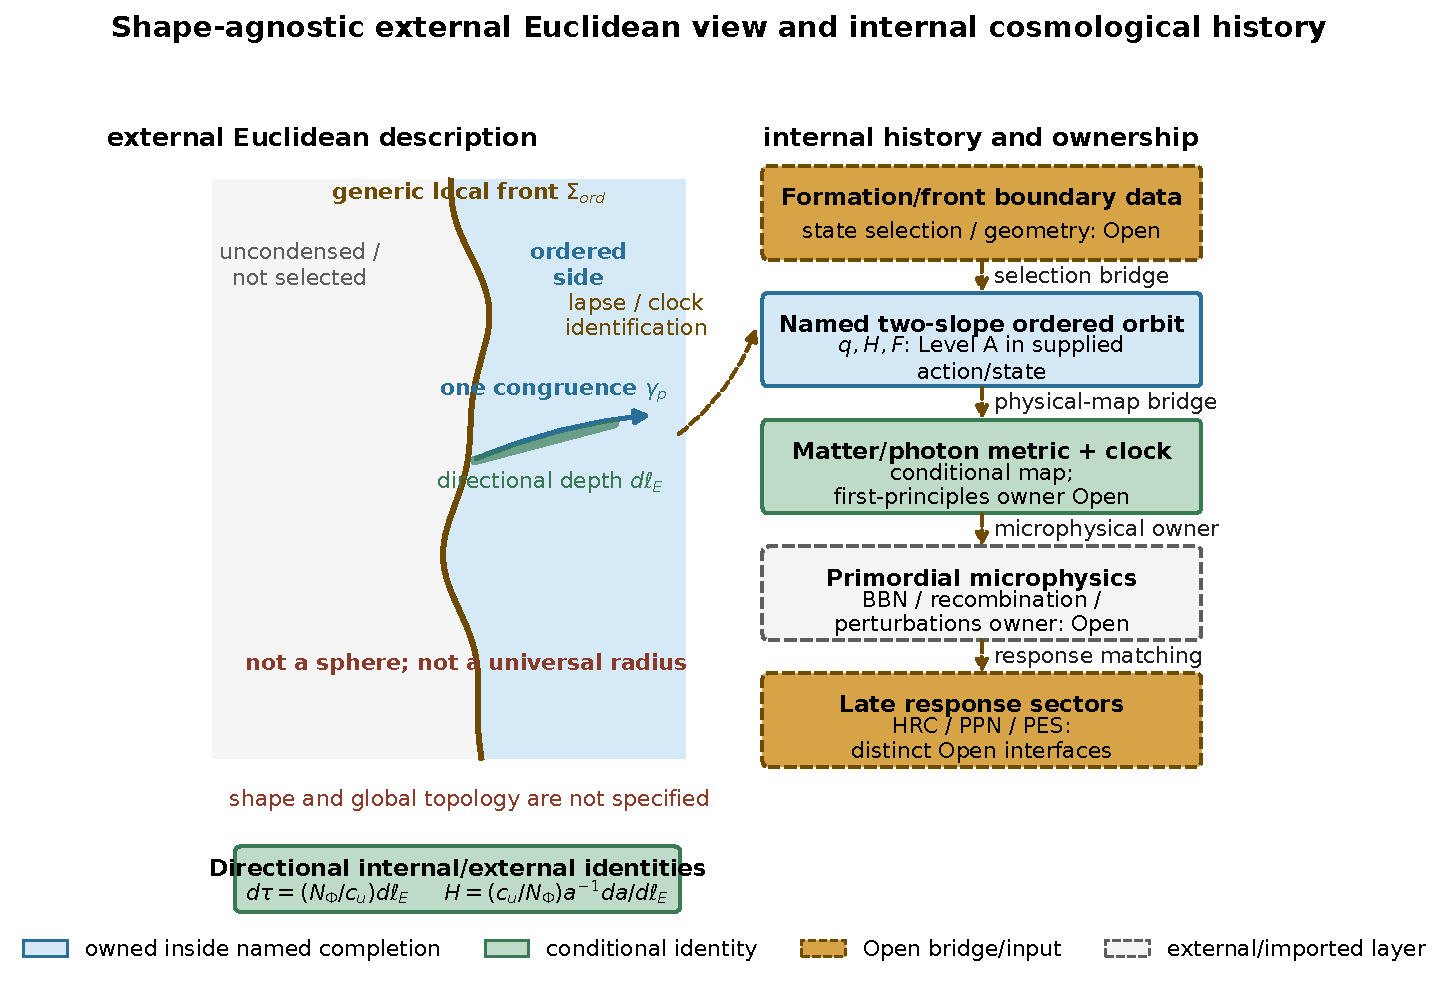
\includegraphics[width=\textwidth]{figures/r149/r149_external_internal_history_map_typography.pdf}
  \caption{\textbf{Shape-agnostic external/internal history map.}
  The external panel depicts a generic local formation front and one
  action-owned congruence, not a spherical boundary.  The internal panel
  separates an orbit that is Level~A only inside the named supplied action/state, a Level~B
  conditional metric/clock map, imported external microphysics, and Open
  interfaces.  Formation/front selection, the first-principles physical
  metric, primordial microphysics, Boltzmann perturbations, HRC/PPN matching
  and PES record kernels remain Open.  Colour follows the luminance-first
  publication status palette and is redundant with border style and literal status
  text.}
  \label{fig:r123_internal_external_history_map}
\end{figure}

\paragraph{Ordering stage.}
The ordering calculation must determine the physical branch, independent
degrees of freedom, defect content, initial entropy and the state inherited
by Lorentzian perturbations.  An equilibrium minimum alone does not determine
the non-equilibrium state or its spectrum.  The output is a boundary-data
functional for the cosmological initial-value problem, not a prescribed
redshift.

\paragraph{Radiation and nucleosynthesis stage.}
The continuation must reach a regime in which the physical photon
temperature, reaction rates, expansion rate and effective gravitational
coupling are calculable.  The BBN forward problem uses
\begin{equation}
 \{H(T_\gamma),m_e(T_\gamma),\alpha_{\rm fs}(T_\gamma),
   \eta_b,N_{\rm eff};\tau_n,\langle\sigma v\rangle_i,
   f_{\nu}(p,T_\gamma),\ldots\}
 \longrightarrow \{Y_p,{\rm D/H},{}^3{\rm He/H},{}^7{\rm Li/H}\}.
 \label{eq:ect_scenario_bbn_map}
\end{equation}
The coefficient $G_{\rm div}$ enters this map only through the action-owned
solved background/response, unless a separate scalar dependence of the
microphysical rates is derived; listing both $H(T_\gamma)$ and an independent
$G_{\rm eff}(T_\gamma)$ would otherwise double-count or leave the transfer
unspecified.
No late-time fit can compensate for failure of this early-state map.

\paragraph{Recombination and structure stage.}
For any proposed completion, the same orbit would have to supply the
expansion and physical couplings used by recombination, while a derived
gauge-reduced quadratic action and primordial state would have to supply the
transfer functions.  Neither owner-complete pipeline is supplied here.  A
claimed early-structure enhancement must be traced to a specific operator in
this chain and checked against CMB spectra, lensing, growth and local gravity.

\paragraph{Late-time stage.}
Acceleration, HRC phenomenology and finite-body screening are presently
distinct candidate descriptions assigned to the same putative medium; their
common action ownership has not been derived.  A viable completion must show
how their scales and couplings coexist without assigning one field coordinate
incompatible roles.  The cosmological Hubble rate is a homogeneous expansion
observable; the HRC argument is a quasistatic acceleration invariant; the
PPN parameters are finite-source metric coefficients.  Equality between any
two scales is a matching hypothesis until the common action derives it.

The supplied regular two-slope action/state supports a quantitative
post-ordering orbit.  This removes the need for the former hand-drawn scalar
history while leaving the transition through the formation front Open.  The
inverse-$F$ curve below is a background diagnostic coordinate and is not
identified with a locally measured Newton constant.

\begin{figure}[!htbp]
  \centering
  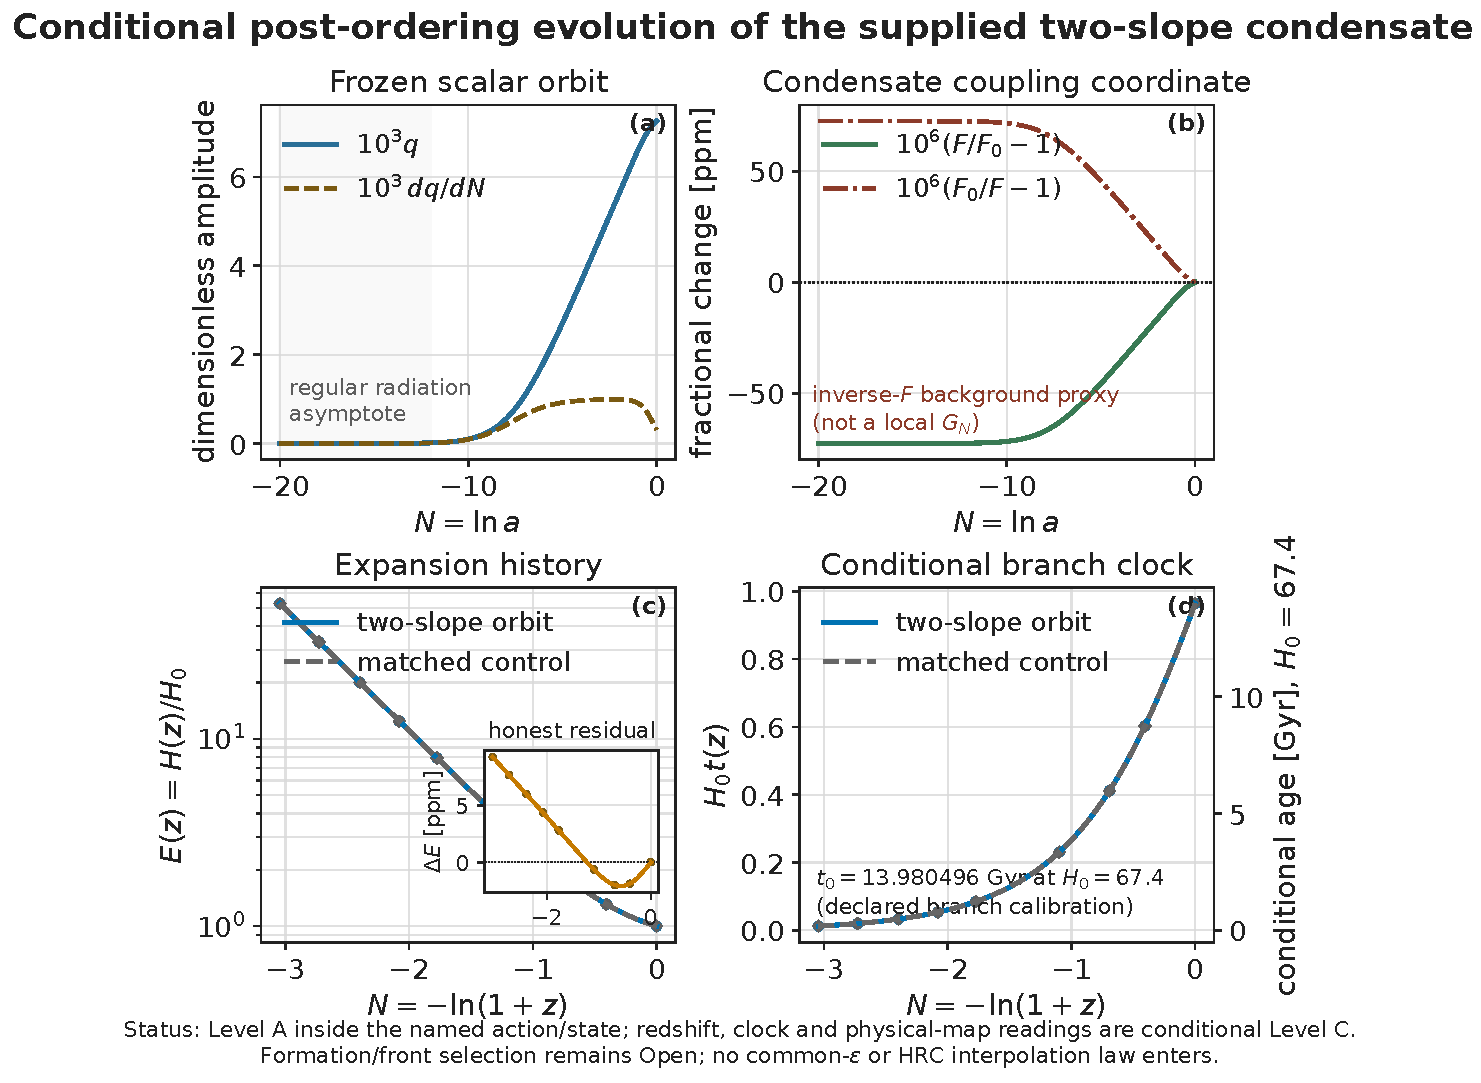
\includegraphics[width=\textwidth]{figures/r154/curve_semantics/nonrotation/conditional_post_ordering_dense_r154.pdf}
  \caption{\textbf{Conditional post-ordering orbit of the supplied
  two-slope scalar completion.}
  Panel (a) shows its scalar coordinate $\sigma$ and velocity
  $d\sigma/dN$ on the frozen regular orbit.  Panel (b) shows $F_s/F_{s0}$
  and the inverse-$F_s$ background proxy, which is not a local $G_N$.  Panel (c) compares the
  action-owned expansion with the same-present-fraction matched control and
  exposes the ppm residual rather than visually exaggerating it.  Panel (d)
  shows the branch clock using the externally supplied reference
  dimensional calibration $H_0=67.4\,
  \mathrm{km\,s^{-1}\,Mpc^{-1}}$.  This calibration is state/data
  input for the displayed history, not a universal P1--P6 prediction.  The dynamical
  curves are Level A only inside the named action/state; redshift, Gyr and
  physical-map readings are conditional Level C.  The integration begins on
  an already ordered regular radiation branch: no trajectory through the
  Open formation front is inferred.  Panels~(c), its inset and~(d) show nine
  evaluated redshift nodes as unconnected markers; no intermediate
  interpolation is implied.  No common-$\varepsilon$ or HRC
  interpolation law enters this figure.  \textit{Display semantics: \detokenize{Panels (a,b) are dense frozen solver histories without decorative markers; panels (c,d) use solver-owned dense background traces with the nine published diagnostic nodes shown separately.}}}
  \label{fig:r123_condensate_orbit}
\end{figure}

\subsection{Matter--antimatter asymmetry in the ECT framework}
\label{sec:baryogenesis}
\label{sec:mp_baryogenesis}
% ============================================================

\textit{Status: Level~C/Open conditional completion.  The discussion below
is an inventory of operators and state assumptions that could realise the
Sakharov conditions; P1--P6 do not yet derive baryon number, a
baryon-violating vertex, a physical CP-odd coefficient, the transition/thermal
state, or the transport and washout system.  Consequently neither
$\eta_B\neq0$ nor its magnitude is presently an ECT prediction.
Connection: Section~\ref{sec:qs_conservation}
(defect-mediated topology change),
Section~\ref{sec:fifth_force} ($\mathcal{L}_5$ coupling),
Section~\ref{sec:u1_emergence} (gauge structure).}

\medskip
In the named base-$\Lambda$CDM Planck likelihood,
$\Omega_bh^2=0.02237\pm0.00015$; the standard conversion
$\eta_{10}\simeq273.9\,\Omega_bh^2$ gives
$\eta_B\simeq(6.13\pm0.04)\times10^{-10}$
\cite{Planck2018}.  This is a model-dependent fit plus conversion, not a
direct count and not ECT evidence.  It corresponds approximately to one net
baryon per billion early particle--antiparticle pairs.
All visible matter---stars, planets, observers---consists of this
surviving excess.

Any baryogenesis mechanism must satisfy the three Sakharov
conditions~\cite{Sakharov1967}: (i)~baryon number violation,
(ii)~C and CP violation, and (iii)~departure from thermal equilibrium.

The development below records a conditional ordered-medium completion in
which supplied owners could implement the Sakharov ingredients.  It is not a
replacement for an explicit gauge, matter and transport calculation.

\subsubsection*{Candidate Sakharov ingredients and missing owners}

\textbf{(i) Baryon number violation: defect-mediated topology change.}

The supplied coherent branch carries integer winding
sectors~(Section~\ref{sec:qs_conservation}).  A defect can change that
collective-field winding when the amplitude vanishes at a core.  This is a
statement about the supplied order parameter, not about physical baryon
number.

Only after supplying a physical gauge/fermion bundle and a map from its
baryon current to this winding could a defect transition represent baryon
violation~(Sections~\ref{sec:u1_emergence}
and~\ref{sec:nonabelian_embedding}).  In an additional defect model one may
then estimate rates such as
\begin{itemize}
  \item in a separately specified thermal state with a derived
    finite barrier $E_{\rm def}$, an Arrhenius regime may give
    $\Gamma_{\rm def}\propto e^{-E_{\rm def}/(k_BT)}$;
  \item outside that regime a rate requires an explicit finite-action
    Euclidean saddle or real-time transition calculation, prefactor and
    state.  Topology alone fixes none of these and does not imply that a
    process becomes unsuppressed at any named ECT scale.
\end{itemize}
These rate forms are illustrative: the defect action, thermal state,
baryon-current map and transition vertex are not derived.  Condensate
topology alone is therefore not an ECT analogue of a physical sphaleron.

\textbf{(ii) CP violation: preferred-direction fermion coupling.}

If fermionic excitations are empirically admitted
(phenomenological input, analogous to $c_{\rm char}=c$),
then the unique leading renormalisable coupling of a spinorial
excitation to the ordered direction field $n_A$ is
\begin{equation}
  \label{eq:baryogenesis_L5}
  \mathcal{L}_5 = \mu_5\,\bar\Psi\gamma^A n_A\Psi
\end{equation}
(Level~A given empirical fermions: EFT uniqueness theorem;
Section~\ref{sec:fifth_force}).
This operator is a candidate ingredient only after a nonzero coefficient,
physical fermion map and branch-state dynamics are supplied.
As systematically classified in
Section~\ref{sec:discrete_symmetries}, $\mathcal{L}_5$ is a
branch-sensitive, CPT-odd and CP-odd phenomenological operator
(C-odd, P-even, T-even, CP-odd, CPT-odd).
Combined with complex phases of the fermionic mass matrix
(open parameter, OP-Yukawa,
Section~\ref{sec:yukawa}), it yields the required CP-asymmetric
dynamics.
Importantly, the conditional CPT route for reconstructible local
sectors identified in
Section~\ref{sec:discrete_symmetries} remains intact: $\mathcal{L}_5$
explicitly lies outside that reconstructible setup as a phenomenological
branch extension, so the exact symmetry backbone of the reconstructible
sectors is not compromised.
The branch-pair architecture of
Section~\ref{sec:discrete_symmetries} additionally admits a
speculative cosmological interpretation in which our observable
matter-dominated branch is paired with an antipodal antimatter-dominated
partner, the full Euclidean pair being CPT-symmetric; this is recorded
as OP-BRANCH1 rather than as an established result.
The complex flavour phases appear explicitly in the flavour-architecture
subsection~(\S\ref{sec:flavour_architecture}), providing the
flavour-sector part of the CP-violation bookkeeping.
The baryogenesis estimate in the present section remains tied to
the leptogenesis-style assumptions stated above and does not claim
that the CKM phase alone explains the observed asymmetry.
In particular, the present framework does not claim that the
observed baryon asymmetry can be generated by the CKM phase alone.

\textbf{(iii) Departure from thermal equilibrium: the ordering
transition.}

P4 supplies an ordered-gradient chart; it does not derive a real-time transition,
its clock map, duration, thermal state, or coupling to physical species.
If a future completion supplies a finite-rate ordering event, species whose
interaction rates are too slow to track it would be out of equilibrium.
If the transition completes on a timescale
$\tau_{\rm tr}\sim M_{\rm Pl}^{-1}$,
then species with $\Gamma\ll\tau_{\rm tr}^{-1}$ would be driven out of
equilibrium.  Both scales in this conditional statement are presently
inputs.

\subsubsection*{Candidate bias operator inventory}

Given the missing owners above, one may write a spontaneous-baryogenesis
candidate rather than derive a bias mechanism.

In a supplied non-equilibrium history, $n_A(X)$ and $\theta(X)$ may be time
dependent.  The following expression is then a candidate operator inventory,
not a derived chemical potential:
\begin{equation}
  \label{eq:mu_eff_baryogenesis}
  \mu_{\rm eff}
  \;\sim\;
  c_\theta\,\dot\theta
  \;+\;
  c_\Omega\,\Omega_t
  \;+\;
  c_5\,\mu_5\,n_0
  \;+\;\cdots
\end{equation}
where $\Omega_t$ is a time-dependent scalar built from the angular
velocity of the ordered frame, and the coefficients
$c_\theta$, $c_\Omega$, $c_5$ depend on the effective Lagrangian of
the coherent branch and on the fermion--condensate coupling structure.

For $\mu_{\rm eff}$ to act as a physical chemical potential, the completed
matter action must couple it to a derived baryon current with the indicated
normalisation.  Only then, and only while an independently derived
baryon-violating process is active, can it source an asymmetry.
In a hot plasma with small $\mu_{\rm eff}/T$, standard
equilibrium thermodynamics gives~\cite{CohenKaplan1988}:
\begin{equation}
  \label{eq:nB_bias}
  n_B - n_{\bar B}
  \;\propto\;
  \mu_{\rm eff}\,T^2.
\end{equation}
After freeze-out at temperature $T_D$, the asymmetry is frozen:
\begin{equation}
  \label{eq:etaB_freezeout}
  \eta_B
  \;\sim\;
  C\,\frac{\mu_{\rm eff}(T_D)}{T_D},
\end{equation}
where $C$ is a model-dependent dimensionless coefficient whose sign and
possible vanishing depend on the charge content, active degrees of freedom,
entropy normalisation, conversion factors, transport and washout details.  It
is not generically of order unity.

\subsubsection*{When matter--antimatter asymmetry arises and when
it does not}

The conditional equations show what a completed model would have to supply;
they do not make a nonzero asymmetry generic.

\paragraph{Necessary ingredients for a conditional $\eta_B\neq0$.}
A nonzero matter--antimatter asymmetry could arise only when the following
conditions are simultaneously realised by the missing action/state:
\begin{enumerate}[label=(\alph*)]
  \item At least one term in Eq.~\eqref{eq:mu_eff_baryogenesis} has an
  action-owned nonzero coefficient and history, producing
  $\mu_{\rm eff}\neq0$, and the completed matter action couples that bias to
  a derived baryon current with fixed normalisation.  Time dependence alone
  does not guarantee a nonzero charge bias.  In particular,
  $\mu_5\neq0$ is necessary only for the director term
  $c_5\mu_5n_0$, not for independent $c_\theta\dot\theta$ or
  $c_\Omega\Omega_t$ routes.
  \item The susceptibility/conversion factor represented by $C$ in
  Eq.~\eqref{eq:etaB_freezeout} is nonzero after charge content, entropy,
  transport and washout are specified.  Its value and sign are not selected.
  \item \emph{B-violating transitions are active} during the epoch
  when the bias is nonzero.
  No such ECT rate has yet been calculated.
  \item \emph{Freeze-out occurs before complete washout}:
  the B-violating rate drops below the expansion rate while
  $\eta_B\neq0$.
\end{enumerate}

\paragraph{Conditions under which $\eta_B=0$.}
The asymmetry vanishes if any of the following conditions
holds:
\begin{enumerate}[label=(\roman*)]
  \item \textbf{Exactly homogeneous transition:}
  the ordering history is sufficiently symmetric that no effective bias
  $\mu_{\rm eff}$ is generated.
  \item \textbf{Vanishing effective CP-bias source:}
  the relevant effective couplings are such that the ordered background
  induces no net CP-asymmetric bias.
  \item \textbf{Vanishing susceptibility or conversion:}
  the completed charge, entropy and transport map gives $C=0$ even when a
  formal $\mu_{\rm eff}$ is nonzero.
  \item \textbf{Exact dynamical cancellation:}
  the bias changes sign during the transition in such a way that the
  integrated asymmetry source cancels.
  \item \textbf{Complete washout:}
  baryon-number-violating processes remain active long enough after the
  bias epoch to erase the produced asymmetry.
\end{enumerate}
None of these is known to be exceptional in the present theory.  Their
relative likelihood cannot be ranked without a measure, transition state
and transport solution.

\subsubsection*{Comparison with the Standard Model}

In the Standard Model, electroweak baryogenesis fails at
observed parameters because the electroweak phase transition is
a crossover rather than a strongly first-order transition.
Additional beyond-minimal ingredients are therefore required for
successful electroweak baryogenesis at the observed parameters.

ECT supplies an ordered $O(4)\to O(3)$ branch, not yet the physical
transition process or its temperature.  The candidate completion above
would add all three Sakharov owners rather than derive them from ordering
alone.  Whether such a completion exists and reproduces the observed
asymmetry is Open.

\subsubsection*{No retained numerical baryogenesis benchmark}

External baryogenesis models span different masses, CP sources, washout
histories and transport systems.  Importing one numerical parameter tuple
would test only that external model and would not constrain the missing ECT
owners.  The present manuscript therefore retains no leptogenesis number as
an ECT consistency check.  The observed $\eta_B$ is only an external target
for a future owner-complete calculation.

\paragraph{Status summary.}
\begin{itemize}
  \item \textbf{Level~A conditional mathematics:}
  integer winding and its possible change through a supplied vanishing-core
  configuration concern the collective order parameter, not baryon number.
  \item \textbf{Conditional EFT candidates:}
  the allowed restricted-basis fermion--condensate
  operator~$\mathcal{L}_5$ can provide a CP-bias candidate only if a
  nonzero coefficient and physical matter map are supplied.  The displayed
  bias and freeze-out equations are standard conditional templates.
  \item \textbf{Open:}
  the physical baryon current and violating vertex, gauge/colour/fermion
  map, CP-odd coefficient, clock and thermal transition state, transport,
  freeze-out, washout, and any ECT value or sign of $\eta_B$.
\end{itemize}

% ============================================================

\subsection{Age of the Lorentzian ordered branch: exact definition and present identifiability}
\label{sec:universe_age}

ECT does not identify cosmic age with elapsed time since a fundamental
singularity.  The physical quantity is the duration of the Lorentzian ordered
branch, beginning at a relational ordering event.  On a monotonically
expanding post-order branch, after the physical photon/matter redshift map has
established $1+z=a_0/a$ and the conventional normalisation $a_0=1$ has been
chosen, the duration at redshift $z$ is the kinematic identity
\begin{equation}
 t_{\rm ECT}(z)=
 \int_{a_{\rm ord}}^{1/(1+z)}{da\over aH_{\rm ECT}(a)},
 \qquad
 t_{0,\rm ECT}=\int_{a_{\rm ord}}^1{da\over aH_{\rm ECT}(a)}.
 \label{eq:ect_age_ordered_branch}
\end{equation}
Equation~\eqref{eq:ect_age_ordered_branch} is Level~A kinematics after
$H_{\rm ECT}(a)$ and $a_{\rm ord}$ are supplied.  It is not by itself a
dynamical prediction of either quantity.

This internal Lorentzian duration $\Delta t_L$ must be distinguished from an
external-Euclidean formation or relaxation parameter.  The clock-zero
surface $\Sigma_{\rm ord}$ may be an internal ordering front, or the
ordered-side portion of an actual finite-condensate boundary if the latter
is what the completed dynamics selects.  The present action has not yet
identified which of these owns the realised branch start.  No assumption of
spherical topology or shape is made in either case.  Three objects must
not be identified without a derivation: the ordered-medium director
\(n^A=\partial^A\Phi/u\), the normal \(s^A\) to the branch-formation front
\(\Sigma_{\rm ord}\), and the physical matter-clock congruence \(U^\mu\).
They coincide in a planar homogeneous special case, but need not do so for a
front defined, for example, by a level set of \(u=|\partial\Phi|\).

For a present event \(p\), let \(\gamma_p\) be the action-owned matter/comoving
curve that intersects the ordered side of the formation front once.  The
outside description of branch age is then the congruence integral
\begin{equation}
 \boxed{\displaystyle
 \tau_{\rm age}(p)=
 \int_{\gamma_p:\,\Sigma_{\rm ord}^{+}\to p}
 {\mathcal N_\Phi[\Phi,\mathrm{matter}](X)\over c_{\rm u}}\,d\ell_E ,
 \qquad d\ell_E^2=\delta_{AB}dX^AdX^B .}
 \label{eq:ect_external_depth_lapse_map}
\end{equation}
The \(+\) indicates that a sharp transition is approached from the ordered
side, where the supplied director exists.  A physical metric, lapse and
matter-clock congruence remain inputs of the completion rather than properties
derived by P4.  Only for
an owned foliation and congruence does the same orbit also give the local
internal--outside differential bridge
\begin{equation}
 d\tau={\mathcal N_\Phi\over c_{\rm u}}\,d\ell_E,
 \qquad
 H_{\rm ECT}={1\over a}{da\over d\tau}
 ={c_{\rm u}\over\mathcal N_\Phi}{1\over a}{da\over d\ell_E}.
 \label{eq:ect_internal_external_hubble_bridge}
\end{equation}
Thus the present Hubble rate and the integrated branch age are two
observables of one state-dependent orbit and lapse map, not independent
adjustable inputs.  Equation~\eqref{eq:ect_internal_external_hubble_bridge}
is a directional congruence identity, not a statement about a radius or a
spherical boundary.  Only for
\(\gamma_p\parallel n^A\parallel s^A\), constant \(\mathcal N_\Phi\), and
planar homogeneous leaves does this reduce to a normal-depth formula
\(\tau_{\rm age}=\mathcal N_\Phi L_w/c_{\rm u}\).  No spherical Universe or
contemporaneous spatial edge is involved.

A local exact director does not by itself provide a global scalar clock.  If
\begin{equation}
 \vartheta={\mathcal N_\Phi\over c_{\rm u}u}\,d\Phi ,
\end{equation}
then a necessary local integrability condition for
\(\vartheta=d\tau\) is
\begin{equation}
 d\!\left({\mathcal N_\Phi\over u}\right)\wedge d\Phi=0.
 \label{eq:ect_global_clock_integrability}
\end{equation}
Without it, age remains well-defined along the specified congruence but may be
a spatial field rather than one global number.  ECT need not select an
absolute Euclidean origin or arbitrary front position; it must derive the
front, crossing rule, congruence and clock response that make
Eq.~\eqref{eq:ect_external_depth_lapse_map} agree with the internal FLRW
integral.  Those owners are presently Open.

\paragraph{Status of the numerical age.}
Universal laws need not select the integration constants and dimensional
calibration of our realised condensate.  Thus an observationally inferred
\(H_0\) may be declared as the single dimensional scale calibration of one
fixed dimensionless orbit after ECT has supplied the physical metric,
redshift map and forward likelihood.  This is a pure rescaling only while no
independently fixed Planck, particle, clock or potential scale has already
fixed the same dimensional normalisation.  What the frozen
postulates and current macroscopic actions do not yet supply is one selected
law-level history together with the physical congruence/depth-lapse map of
Eq.~\eqref{eq:ect_external_depth_lapse_map}.  Therefore
\begin{equation}
 \boxed{H_{\rm ECT}(a)\ \hbox{and}\ t_{0,\rm ECT}
 \ \hbox{are calculable for a named action/state, but are not uniquely
 selected by P1--P6}.}
 \label{eq:ect_age_not_identifiable}
\end{equation}
Conditional gigayear estimates for explicitly supplied completions are given
in Section~\ref{sec:two_slope_background_proof_class}.  What is not identified
at the present closure level is one unique law-level age; this is not a claim
that legitimate state data or one dimensional scale calibration are defective.

\paragraph{Exact reason: inverse reconstruction of the scalar closure.}
For the scalar-only background equations
\begin{align}
3FH^2&={\rho_m+\rho_r+U\over\bar M_{\rm Pl}^2}
       +\frac12\omega\dot\phi^2-3H\dot F,\nonumber\\
-2F\dot H&={\rho_m+\tfrac43\rho_r\over\bar M_{\rm Pl}^2}
       +\omega\dot\phi^2+\ddot F-H\dot F,
\label{eq:ect_age_background_pair}
\end{align}
let $H(t)$ and $F(t)>0$ be sufficiently smooth and let ordinary matter and
radiation be conserved.  Define
\begin{align}
 \mathcal K(t)&\equiv\omega\dot\phi^2
 =-2F\dot H-{\rho_m+\tfrac43\rho_r\over\bar M_{\rm Pl}^2}
 -\ddot F+H\dot F,
 \label{eq:ect_age_inverse_kinetic}\\
 {U(t)\over\bar M_{\rm Pl}^2}
 &=3FH^2+F\dot H+\frac12\ddot F+\frac52H\dot F
 -{\rho_m\over2\bar M_{\rm Pl}^2}
 -{\rho_r\over3\bar M_{\rm Pl}^2}.
 \label{eq:ect_age_inverse_potential}
\end{align}
Direct substitution makes both equations in
\eqref{eq:ect_age_background_pair} identities.  On every patch where
$F=e^{\beta_\phi\phi}$ is monotonic and $\dot\phi\ne0$, one has
$\phi=\beta_\phi^{-1}\ln F$ and obtains $\omega(\phi)$ and $U(\phi)$ by
composition with $t(\phi)$, provided
$\omega=\mathcal K/\dot\phi^2$ is finite and has the required physical sign.
The scalar equation follows only with the corresponding Bianchi identity and
conserved matter/radiation stress tensor; a zero of $\dot\phi$ requires a new
patch or a separate regular-variable construction.  Thus the currently
unowned closure
functions can support a continuum of expansion histories.  This is an exact
non-identifiability theorem inside the displayed scalar equations; it is not
a failure of a numerical integrator.

\paragraph{Constructive boundary of the theorem.}
Non-identifiability does not mean that every nearby scalar completion is
singular.  Section~\ref{sec:two_slope_background_proof_class} gives an
explicit two-slope action with exact radiation and dust limits, a stable
vacuum and globally regular two-solver trajectories.  Its near-GR member has
$\tau_{2s}\equiv H_{2s}(0)\Delta t=0.96368677864$ without a background splice.
Two disclosed single-scale calibrations of the same dimensionless orbit give
$13.98050$ or $12.90095$~Gyr.  These are conditional ages of a named
calibrated ECT-compatible candidate completion.
Universal laws need not fix one state-specific number; what remains binding
in Eq.~\eqref{eq:ect_age_not_identifiable} is the Open microscopic selection
and physical metric/clock/front map, not any demand for a universal age.

\paragraph{Additional independent missing owners.}
Even after choosing the scalar functions, the physical age still requires:
\begin{enumerate}[label=(\roman*)]
 \item a stationary ordered-phase action---the P4 gradient background is not
       stationary under the frozen bare P3 action;
 \item the covariant orientation action and its homogeneous stress tensor;
 \item a non-circular metric and Planck-scale matching from $(u,n_A)$;
 \item the physical state, matter/radiation abundances, branch and boundary
       data;
 \item the external-depth/lapse map that turns the ordering-front evolution
       into the start and duration of the Lorentzian matter clock;
 \item stability, Newtonian, PPN and perturbation gates for the same solution.
\end{enumerate}

\paragraph{What the external Euclidean view does and does not add.}
No spherical boundary is assumed.  On an arbitrary smooth interface the
full flat-boundary massive Euclidean Dirichlet-to-Neumann symbol is
$\sqrt{M^2+|\xi|_h^2}$.  In the ordinary classical high-frequency expansion
its homogeneous principal symbol is $|\xi|_h$; the mass enters at lower order,
while curvature-dependent subprincipal and lower terms depend on the second
fundamental form $K_{ij}$.  Boundary shape and state therefore cannot
be replaced by one global radius.  A uniform translation of a flat interface
is an ambient Euclidean isometry and has $\dot\Lambda=0$; it cannot simply be
renamed Hubble expansion.  Moreover, identifying
$K_{ij}=(H/c)h_{ij}$ with a spatially flat codimension-one FLRW slice in
flat $E^4$ violates the Gauss equation unless $H=0$.  A distinct response
fibre, curved ambient completion, higher codimension, or derived director
invariant is required.  The outside view therefore sharpens the missing
geometric owners but does not supply an age for free.

\paragraph{Age, lookback time, and early objects.}
Once a unique background exists, lookback and formation intervals follow
from the same solution,
\begin{align}
 t_{\rm lookback}(z)&=\int_{1/(1+z)}^1{da\over aH_{\rm ECT}(a)},\\
 t_{\rm gal}(z_{\rm obs};z_{\rm form})
 &=\int_{1/(1+z_{\rm form})}^{1/(1+z_{\rm obs})}
   {da\over aH_{\rm ECT}(a)}.
\end{align}
These formulae do not establish a JWST time budget until the same derived
$H_{\rm ECT}$ is coupled to a perturbation, halo-formation and baryonic
forward model.  An external high-redshift history may not be grafted onto the
solution, and the dimensional calibration may not be changed independently
between observables.  After the complete dimensionless ECT orbit has been
solved, a measured $H_0$ may be declared once as a single dimensional scale
calibration of that same dimensionless orbit,
with that status carried through every clock and distance output.

\paragraph{Falsifier and completion criterion.}
A conditional ECT age is calculable once one complete varied action, one
physical state, one ordering-front/depth-lapse map, dimensional unit data and
one self-consistent background integration are supplied.  It becomes an
independent prediction only to the extent that some of those state data are
fixed by other observables and the remaining age or Hubble quantity follows.
ECT need not make the realised age a universal constant: $H_0$ and age may be
legitimate observed descriptors of our condensate state.  What is mandatory
is that one orbit, one dimensional scale calibration and one lapse map impose
the dimensionless combination
$H_0^{\rm cal}t_0$ after the declared calibration and the full correlated
clock--distance history.  Different stable
closures or depth/lapse maps that pass their own assumptions but yield
materially different correlations demonstrate that the dynamical closure,
not the concept of state data, remains underdetermined.


\subsection{ECT cosmological background: owners, observables, and closure gates}
\label{sec:ect_cosmology_closure}

The cosmological sector is organised by physical owners.  The Hubble, JWST,
chronometer, growth, lensing and ISW questions are assigned to the dynamical
operators that actually control them rather than to one shared empirical
parameter.

\paragraph{The action-to-observable chain.}
A cosmological prediction requires the ordered sequence
\begin{equation}
 \boxed{
 S_{\rm ECT}^{\rm cov}
 \longrightarrow
 \{H(a),\phi(a),n_A(a),\rho_i(a)\}
 \longrightarrow
 \{\delta_i,\Phi_{\rm W},\mathcal R\}
 \longrightarrow
 \{D_A,r_s,f\sigma_8,C_\ell,\mathcal N_{\rm halo},\gamma_{\rm PPN},\beta_{\rm PPN}\}.}
 \label{eq:ect_cosmo_action_observable_chain}
\end{equation}
Every arrow must be owned by the same varied action and state.  A static HRC
response law does not replace the homogeneous background or its perturbation
completion: the comoving FLRW congruence has vanishing proper acceleration,
so the HRC acceleration invariant is zero on the exact homogeneous solution.

\paragraph{Currently controlled equations.}
Inside the supplied scalar-only Jordan-frame model, variation yields the
background equations collected in
Eqs.~\eqref{eq:bg_reduction_friedmann}--\eqref{eq:bg_reduction_scalar}.
Their algebra is exact inside that model.  Their ownership by ECT remains
Level~B/Open because $F$, $\omega$, $U$, the orientation action and the state
are not fixed by P1--P6.  The inverse-reconstruction theorem of
\S\ref{sec:universe_age} proves that these missing functions are sufficient
to support inequivalent $H(a)$ histories.

\begin{longtable}{@{}L{2.55cm}L{3.45cm}L{5.00cm}L{3.65cm}@{}}
\caption{Owner map for the active ECT cosmology programme.}
\label{tab:ect_cosmology_owner_map}\\
\toprule
Target & Required dynamical owner & Present disposition & Status\\
\midrule
\endfirsthead
\toprule
Target & Required dynamical owner & Present disposition & Status\\
\midrule
\endhead
Physical background $H(a)$ & Complete covariant ordered-phase action,
state and initial/boundary data & Exact inverse reconstruction proves that
P1--P6 do not select one history; a named two-slope completion supplies one
regular conditional $H(a)$ and a nine-point parameter scan & A inside named
action / B proof of class / C diagnostics / Open P1--P6 ownership\\
ECT age & Named action/state, physical matter congruence, external
depth/lapse map and one declared dimensional calibration & Exact quadrature;
$\tau_{2s}\equiv H_{2s}(0)\Delta t=0.96368678$ and disclosed Gyr conversions
for one two-slope state; the official 15-point BC03 covariance calibrates the
same orbit to $H_0=68.59\pm3.95$ and $t_0=13.74\pm0.79$~Gyr.  State data and
one dimensional calibration are legitimate inputs, while the physical map
and microscopic completion remain Open & A/C/Open\\
Hubble inference & Recombination, photon metric, $r_s$, $D_A$ and late
distance ladder in one likelihood & Conditional $H(z)$, $D_M$, imported-
recombination $r_s$ and a covariance-aware 15-point chronometer scale
calibration computed; no ECT-native joint early+late likelihood & C/Open\\
JWST abundances & Background age/volume, primordial spectrum, transfer,
non-linear halo and baryonic selection model & Conditional high-$z$ clock
budgets computed at nine prespecified parameter nodes; all nine give
$\Delta t(z{=}10)<0$ relative to the declared control, with the most negative
sampled shift $-10.491167\%$; no continuous-family, abundance, or morphology
conclusion & C/Open\\
Linear growth & Gauge-complete scalar/vector/tensor perturbation action,
matter coupling, slip and sound speeds & Restricted quasistatic
$\mu_{\rm QS}=F_0/F$ diagnostic computed; full kernel and likelihood Open & C/Open\\
ISW and lensing & Photon metric and Weyl-potential transfer & Restricted
same-metric, zero-slip, quasistatic Weyl-amplitude and derivative carriers
computed; projected spectra and horizon-scale ISW remain unowned & C/Open\\
Clusters and mergers & Non-local/retarded metric response plus collision and
baryonic forward model & A strictly increasing local map preserves the
set-valued argmax and cannot move an attained total-response maximizer away
from the supplied total-baryon maximizers; one common real
Debye pole plus ballistic transport is conditionally excluded; inherited
gas/BCG offsets and residual extrema lie outside the local theorem & Level A
theorem in supplied map / conditional Level A one-pole /
physical cluster map Open\\
Solar System / PPN & Covariant weak-field metric completion around a finite
source & Scalar cone or galactic response alone does not determine
$(\gamma_{\rm PPN},\beta_{\rm PPN})$ & Open\\
\bottomrule
\end{longtable}

\paragraph{Hubble tension.}
The observable is not a direct function of one late-time coupling.  It
requires the sound horizon
\begin{equation}
 r_s(z_*)=\int_{z_*}^{\infty}{c_s(z)\over H_{\rm ECT}(z)}\,dz
\end{equation}
together with the angular-diameter distance, recombination history, photon
metric and the late distance-ladder likelihood.  Until those are derived and
fitted in one pipeline, ECT neither resolves nor uniquely predicts the
magnitude or sign of the inferred $H_0$ shift.  For the supplied near-GR
two-slope state, Table~\ref{tab:two_slope_background_observables} gives
$H(z)$ and distance directly, while
Eq.~\eqref{eq:two_slope_conditional_sound_horizon} gives an
imported-recombination diagnostic: $\Delta r_s/r_s=-0.00316\%$.  This is a
conditional diagnostic of that supplied action/state plus imported
recombination, not an ECT prediction of $H_0$; the named state generates no
material shift within those assumptions.

\paragraph{JWST early massive objects.}
An early-object prediction needs the derived time and volume elements, the
primordial perturbation spectrum, transfer functions, scale-dependent growth,
collapse statistics, stellar mass-to-light modelling and survey selection.
Changing only a background coupling or age does not establish an abundance,
morphology or formation history.  The current ECT result is a programme with
explicit owners plus conditional clock budgets, not a claimed resolution.
At the nine prespecified nodes in
Table~\ref{tab:two_slope_calibrated_scan}, stronger sampled departures reduce
$t(z{=}10)$ by as much as $10.491167\%$ while increasing the homogeneous
Planck drift.  Hence none of those nine background nodes enlarges the sampled
$t(z=10)$ age budget.  This finite-grid result is neither a theorem
over the continuous two-parameter family nor a JWST abundance no-go; unsampled
background regions and distinct perturbative/nonlinear mechanisms remain Open
and must pass the same clock and local-gravity gates.

\paragraph{Growth, ISW and cosmological lensing.}
The relevant quantities are obtained from the quadratic action for physical
perturbations and the metric seen by matter and photons.  A future completion
must derive a Poisson kernel, gravitational slip, all physical sound speeds,
anisotropic stress and initial conditions.  Only then can it predict
$f\sigma_8$, the Weyl potential, ISW cross-correlations and weak-lensing
spectra.  Importing a multiplicative growth factor is not an ECT calculation.
Equation~\eqref{eq:two_slope_growth_diagnostic} is a named
quasistatic approximation: it gives sub-$2\times10^{-3}\%$ changes in the
near-GR state and is not a substitute for the gauge-reduced calculation.

\paragraph{HRC and cosmology.}
HRC supplies a candidate quasistatic response in the galactic
mass-discrepancy sector after a separate gravity bridge.  It does not supply
the stress tensor of the homogeneous condensate or the cosmological
perturbation action.  A relation such as $a_M\propto cH$ is an independently
testable matching hypothesis until a single action makes both sides outputs.
Critical interface response may reduce HRC owner classes, but it does not by
itself determine $H(a)$.

\subsubsection*{Conditional cosmology from a supplied action and state}

The calculation uses a family of complete scalar actions and states whose
equations are integrated from
radiation domination to the present.  For the calibrated slice
\begin{equation}
 c_s=a_s,\qquad b_s=3a_s,\qquad
 {V_-\over V_+}={b_s-2a_s\over2a_s-c_s}=1,
 \qquad \sigma(0)=0,\qquad H(0)=H_*,
 \label{eq:two_slope_calibrated_family}
\end{equation}
the last two conditions are shooting targets, not fitted observables.  The
scan uses $\Omega_{m0}=0.315$, $\Omega_{r0}=9.19\times10^{-5}$ and starts at
$N=-20$ with $\sigma'=0$.  Every point below was integrated independently
with DOP853 and Radau.  Their dimensionless ages agree within
$1.4\times10^{-15}$; $F_s$, $H^2$, the Friedmann denominator and the reduced
response determinant remain positive on the sampled trajectories.

\begingroup
\setlength{\LTleft}{0pt}
\setlength{\LTright}{0pt}
\begin{longtable}{@{\extracolsep{\fill}}c c r r r r r r@{}}
\caption{Conditional calibrated two-slope family.  The sound horizon uses
the explicitly imported standard photon/recombination layer
$\Omega_b=0.0493$, $\Omega_\gamma=5.45\times10^{-5}$ and
$z_{\rm drag}=1059.94$; the displayed $H_0^{(\theta_*)}$ is only the rough
fixed-acoustic-angle rescaling
$67.4\,r_s^{\rm ctl}/r_s^{2s}$, not an ECT likelihood result.  The displayed
early-to-present ratio is the divided coefficient
$G_{{\rm div},s}^{\rm early}/G_{{\rm div},s}^{0}
=F_s(0)/F_{s,\rm early}$; it is not by itself a BBN or locally measured
gravity response.}
\label{tab:two_slope_calibrated_scan_expanded}\\
\toprule
$a_s$&$\kappa_s$&
$\Delta t_0$ [\%]&$\Delta t_{10}$ [\%]&
$\Delta r_s$ [\%]&$G_{{\rm div},s}^{\rm early}/G_{{\rm div},s}^{0}$&
$|\gamma_{\rm PPN}-1|$&$H_0^{(\theta_*)}$\\
\midrule
\endfirsthead
\toprule
$a_s$&$\kappa_s$&
$\Delta t_0$ [\%]&$\Delta t_{10}$ [\%]&
$\Delta r_s$ [\%]&$G_{{\rm div},s}^{\rm early}/G_{{\rm div},s}^{0}$&
$|\gamma_{\rm PPN}-1|$&$H_0^{(\theta_*)}$\\
\midrule
\endhead
\bottomrule
\endfoot
0.01&0.05& 0.003321& -0.19304& -0.64208&1.01502&$1.9920\,10^{-3}$&67.836\\
0.03&0.05& 0.029258& -1.69939& -5.54599&1.14110&$1.7375\,10^{-2}$&71.357\\
0.08&0.05& 0.181262&-10.49117&-30.64606&2.32553&$1.0191\,10^{-1}$&97.183\\
0.01&1   & 0.000166& -0.00968& -0.03226&1.00075&$9.9980\,10^{-5}$&67.422\\
0.03&1   & 0.001497& -0.08700& -0.28977&1.00674&$8.9838\,10^{-4}$&67.596\\
0.08&1   & 0.010565& -0.61396& -2.03130&1.04864&$6.3191\,10^{-3}$&68.797\\
0.01&10  & 0.000017& -0.00097& -0.00323&1.00007&$9.9998\,10^{-6}$&67.402\\
0.03&10  & 0.000150& -0.00871& -0.02904&1.00067&$8.9984\,10^{-5}$&67.420\\
0.08&10  & 0.001065& -0.06189& -0.20620&1.00479&$6.3918\,10^{-4}$&67.539\\
\end{longtable}
\endgroup

\begin{figure}[p]
\centering
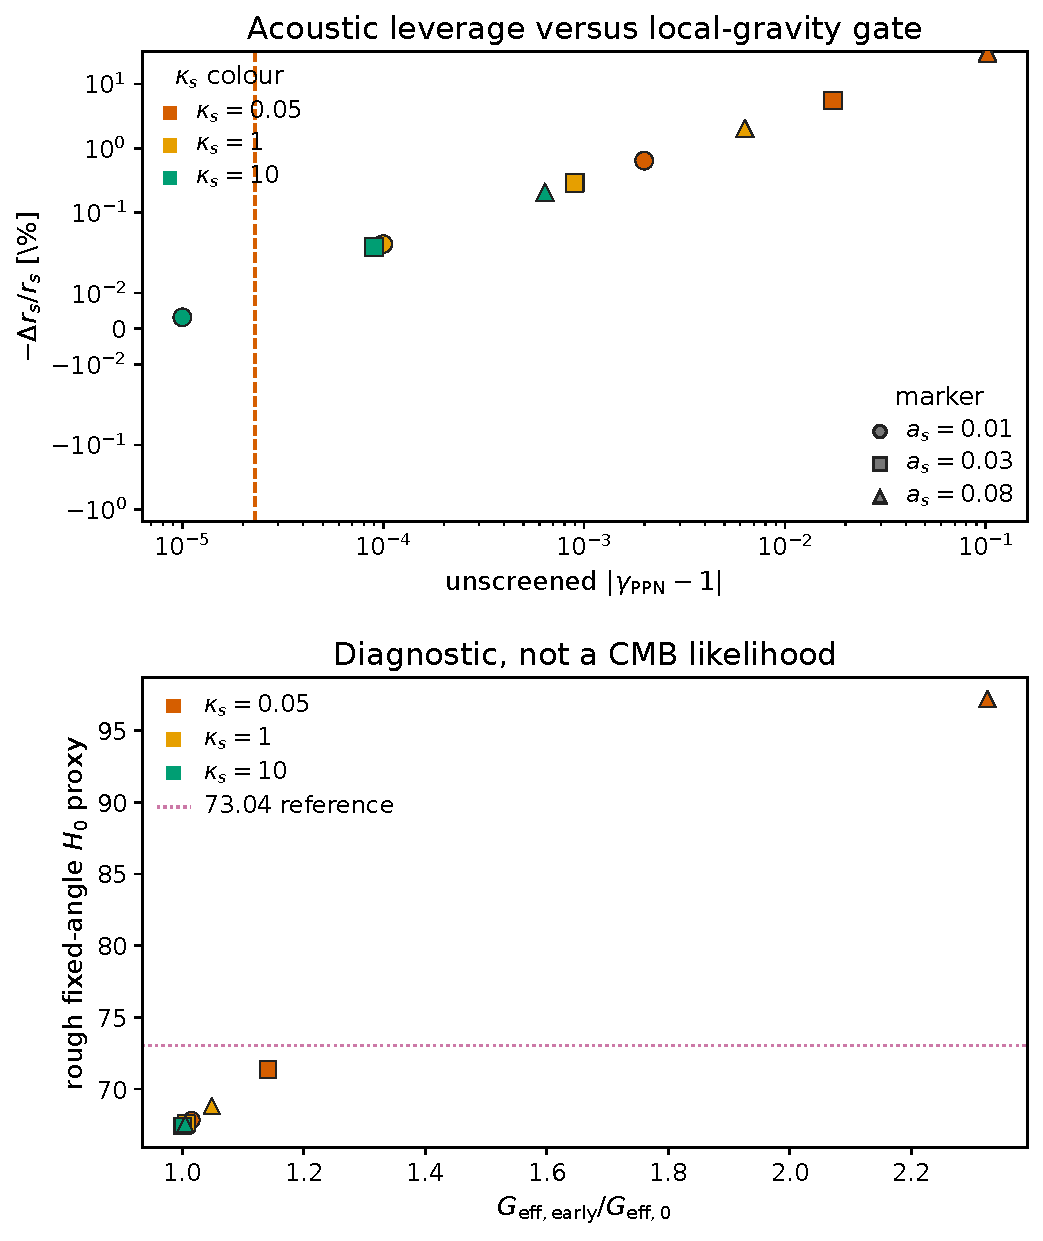
\includegraphics[width=\textwidth,height=0.76\textheight,keepaspectratio]{figures/r153/line_semantics/acoustic_ppn_nodes_r153.pdf}
\caption{Conditional nine-point two-slope acoustic--PPN scan.  This
page shows acoustic leverage against the exact unscreened massless-scalar PPN
gate of the same supplied action/state.  The rough fixed-acoustic-angle
diagnostic is a separate full-width atlas panel and is not a CMB or
distance-ladder likelihood.  The nine independently computed parameter nodes
are shown without connecting segments: no fit or continuously evaluated
parameter path is implied.  Okabe--Ito colours and the $a_s$ marker shapes
provide redundant encodings.}
\label{fig:r103_ect_acoustic_ppn_tradeoff}
\end{figure}
\par\smallskip\noindent The corresponding fixed-acoustic-angle proxy is retained in Appendix~\ref{app:r129_visual_acoustic_cluster_gates}.

\paragraph{What this scan establishes.}
It establishes, at Level~A inside each supplied action/state, that regular
background trajectories exist and that the age, high-redshift clocks, sound
horizon and long-range scalar response can be propagated from the same
orbit.  As a Level~C completion scan it also exposes a tradeoff: the points
with the largest reduction of $r_s$ and largest rough upward acoustic
rescaling of $H_0$ simultaneously have large early divided-coefficient shifts
and fail the unscreened massless-scalar PPN limit.  The column
$G_{{\rm div},s}^{\rm early}/G_{{\rm div},s}^{0}$ records Planck-coefficient
bookkeeping, not a BBN, Cavendish or finite-body response.  This is not a
universal no-go for ECT, but the same action's finite-body calculation below
finds no mass-screening regime for the named calibration.  The strongly
coupled rows therefore require a different derived response or metric
completion; they cannot borrow suppression from this scalar mechanism.

\paragraph{Exact local-gravity diagnostic for this family.}
For this explicitly specified unscreened constant-exponential benchmark
only---not as a universal ECT prediction---the Einstein-frame scalar coupling
is constant and
\begin{equation}
 \omega_{\rm BD}={\kappa_s\over a_s^2},\qquad
 \gamma_{\rm PPN}={\omega_{\rm BD}+1\over\omega_{\rm BD}+2}
 ={\,\kappa_s+a_s^2\,\over\,\kappa_s+2a_s^2\,},\qquad
 \beta_{\rm PPN}=1 .
 \label{eq:two_slope_unscreened_ppn_summary}
\end{equation}
For this same massless, universally coupled weak-body limit,
\begin{equation}
 \alpha_s^2={a_s^2\over2\kappa_s+3a_s^2},\qquad
 G_{{\rm div},s}={1\over8\pi F_s},\qquad
 G_{{\rm Cav},s}=G_{{\rm div},s}(1+\alpha_s^2)
 ={1\over8\pi F_s}{2\kappa_s+4a_s^2\over2\kappa_s+3a_s^2}
 \quad(c=\hbar=1).
 \label{eq:two_slope_Gcav_transfer}
\end{equation}
Because $\alpha_s$ is constant along each scan row, the early-to-present
$G_{{\rm Cav},s}$ ratio equals the corresponding $F_s^{-1}$ ratio only in
this explicitly unscreened massless weak-body limit.  A finite scalar range,
body charges or screening changes the transfer; the ratio is not thereby an
LLR or BBN observable.
Only $(a_s,\kappa_s)=(0.01,10)$ satisfies the manuscript's displayed absolute
proxy gate $|\gamma-1|<2.3\times10^{-5}$ in this unscreened massless limit.
The primary Cassini result is
$\gamma-1=(2.1\pm2.3)\times10^{-5}$~\cite{Bertotti2003}; the conditional
proxy value
$\gamma-1=-0.99998\times10^{-5}$ lies $1.3478\sigma$ from that central value,
outside the literal one-sigma interval but inside two sigma.  Thus the row
satisfies only the declared absolute-deviation proxy gate, not a full Cassini
likelihood or a complete ECT PPN fit.

\paragraph{Hubble-channel consequence.}
The fixed-$\theta_*$ values in
Table~\ref{tab:two_slope_calibrated_scan_expanded} are a transparent
one-number diagnostic, not a posterior.  They hold the reference acoustic
angle fixed while changing only the conditional sound horizon.  A valid
ECT inference must recompute recombination, $D_M(z_*)$, diffusion damping,
the perturbation spectra and the late distance ladder.  Nevertheless the
diagnostic is useful: the only scan point that passes the displayed absolute
$\gamma$ proxy gate moves the rough value by merely $0.002$
km\,s$^{-1}$\,Mpc$^{-1}$.
Among the nine computed nodes, those with
$H_0^{(\theta_*)}\simeq71.4$ or $97.2$ fail the displayed unscreened
$\gamma_{\rm PPN}$ proxy and have large homogeneous divided-coefficient
ratios,
$G_{{\rm div},s}^{\rm early}/G_{{\rm div},s}^{0}=1.14110$ and $2.32553$.
No separately defined ``early-Planck-scale gate'' was evaluated; these ratios
are not BBN observables, and BBN/recombination viability requires the forward
calculation specified above.

\paragraph{Early-object consequence.}
None of the nine evaluated background nodes enlarges the sampled
$t(z=10)$ age budget; the largest sampled departure makes that age
smaller by $10.491167\%$.  This is an exact result for the finite
protocol, not a theorem over the continuous two-parameter family and not a
JWST abundance no-go.  An ECT explanation of early massive objects would need
either an as-yet untested viable background region or a derived change in the
primordial spectrum, scale-dependent transfer/growth, collapse efficiency or
baryonic assembly, all propagated through the same local and recombination
gates.

\subsubsection*{Observable-by-observable calculation protocols}

\paragraph{Chronometers and ages.}
For each action/state point the publication object is the ordered tuple
\begin{equation}
 \mathcal O_{\rm age}=
 \{H(N_i),\,H_0^{\rm cal}t(N_i),\,H_0^{\rm cal}t_0,\,
 \mathcal N_w(w),\,\mathcal C_{\rm bg}(N_i)\}.
 \label{eq:ect_age_publication_object}
\end{equation}
Here \(\mathcal C_{\rm bg}\) is the full constraint residual and
\(\mathcal N_w\) is the external-depth/lapse map of
Eq.~\eqref{eq:ect_external_depth_lapse_map}.  Gyr values are secondary
products obtained only after one dimensional scale calibration of the fixed
state/orbit.  The same \(H(z)\)
array must be used for chronometers, distances and early-object clocks;
independent interpolants are not permitted.

\paragraph{Distance-ladder and BAO chain.}
Starting from the physical photon metric, the solver publishes
\(D_M,D_A,D_L,dV_c/(dz\,d\Omega)\) and \(r_{\rm drag}\) on one common
grid.  The dimensionless likelihood inputs are
\begin{equation}
 {D_M(z)\over r_{\rm drag}},\qquad
 H_\gamma(z)r_{\rm drag},\qquad
 m_B-M_B-5\log_{10}D_L(z),\qquad
 D_L^{\rm GW}(z),
 \label{eq:ect_late_distance_likelihood_inputs}
\end{equation}
with the calibration covariance and possible matter--photon--tensor metric
differences explicit.  A reference \(r_{\rm drag}\) may be used only as the
labelled diagnostic in Table~\ref{tab:two_slope_calibrated_scan_expanded};
it cannot enter an ECT likelihood.

\paragraph{Recombination and CMB chain.}
The background is coupled to a recombination solver through the physical
electron mass, fine-structure constant, Thomson opacity and photon
temperature.  The required residual vector is
\begin{equation}
 \mathbf R_{\rm CMB}=
 \{\theta_*,\theta_{\rm diff},z_*,z_{\rm drag},
 C_\ell^{TT},C_\ell^{TE},C_\ell^{EE},C_L^{\phi\phi}\}_{\rm ECT}
 -
 \{\mathcal D\}_{\rm obs}.
 \label{eq:ect_cmb_residual_vector}
\end{equation}
No single component can be minimised by changing a parameter that is kept
fixed in the other components.  The ECT action/state hash and the
external-depth/lapse map accompany every transfer file.

\paragraph{Optional low-multipole completion target.}
An ordering/coherence scale can motivate asking whether a future completed
primordial state modifies only the lowest wavenumbers; it does not determine
the sign, amplitude or shape of that modification.  A named Open ansatz may,
for example, declare
\begin{equation}
 \begin{aligned}
 \mathcal P_{\mathcal R}(k)
   &=\mathcal P_{\rm ref}(k)\bigl[1-A_LW(k/k_c)\bigr],\\
 k_c&>0,\qquad W:[0,\infty)\to[0,1],\\
 W(0)&=1,\qquad \lim_{x\to\infty}W(x)=0,
       \qquad 1-A_LW(k/k_c)\ge0.
 \end{aligned}
 \label{eq:optional_low_ell_window}
\end{equation}
where $A_L$, $k_c$ and the low-pass window $W$ are independently supplied.
Unless a window family is fixed, its shape and $k_c$ are not separately
identifiable from this parametrisation.  The usual
transfer relation
\begin{equation}
 C_\ell^{XY}=4\pi\!\int d\ln k\,
 \mathcal P_{\mathcal R}(k)\Delta_\ell^X(k)\Delta_\ell^Y(k)
 \label{eq:optional_low_ell_transfer}
\end{equation}
then becomes calculable only after a common gauge-invariant perturbation
action, state, recombination/Boltzmann transfer and likelihood are supplied.
$A_L>0$ would describe suppression inside this ansatz, but P1--P7 selects
neither $A_L>0$ nor any quadrupole value.  Thus the low-$\ell$ branch is a
C/Open completion target, not an ECT prediction, explanation or evidence.

\paragraph{Growth and redshift-space distortions.}
The conditional quasistatic result in
Eq.~\eqref{eq:two_slope_growth_diagnostic} is retained because it is a
reproducible limiting calculation, but it is not promoted into the physical
growth curve.  The full calculation begins from the reduced kinetic,
gradient and mass matrices, evolves all adiabatic and isocurvature modes,
and publishes
\begin{equation}
 \mathcal O_{\rm gr}=
 \{T_m(k,z),T_\theta(k,z),\mu_{\rm cos}(k,z),
 \eta_{\rm slip}(k,z),P_{\rm lin}(k,z),P_\ell^{s}(k,z)\}.
 \label{eq:ect_growth_publication_object}
\end{equation}
Only a covariance-weighted fit of these quantities can establish a growth
or \(S_8\) result.  Multiplying a reference growth curve by one background
number is not an ECT calculation.

\paragraph{Lensing and ISW.}
The metric bridge must determine the Weyl potential
\(\Phi_{\rm W}=(\Phi+\Psi)/2\) seen by photons.  The jointly owned targets
are
\begin{equation}
 C_\ell^{\kappa\kappa},\quad
 C_\ell^{g\kappa},\quad
 C_\ell^{Tg}\big|_{\rm ISW},\quad
 C_L^{\phi\phi},\quad
 D_L^{\rm GW}/D_L^\gamma .
 \label{eq:ect_weyl_target_set}
\end{equation}
A background scalar coupling does not determine any of these without the
slip and transfer system.  A local HRC relation is likewise insufficient.

\paragraph{JWST abundance and morphology.}
For a frozen survey selection \(\mathcal S\), a calculable ECT prediction is
\begin{equation}
 {dN\over dz\,dM_*\,d\Omega}
 = {dV_c\over dz\,d\Omega}
 \int dM_h\,{dn_h\over dM_h}
 P(M_*|M_h,z)\,\mathcal S(M_*,z),
 \label{eq:ect_jwst_forward_count}
\end{equation}
together with image-level size and morphology likelihoods.  The halo mass
function must be generated from the ECT linear spectrum and a validated
non-linear collapse calculation.  The conditional time budgets constrain
the integral's possible histories but do not replace it.

\paragraph{Clusters and collision lensing.}
The local-HRC theorem fixes a narrower baseline: a strictly increasing
pointwise transformation preserves the set-valued argmax and, whenever maxima
are attained, cannot displace a total-response maximizer relative to the
maximizers of the supplied total projected baryon proxy.  Any gas/BCG
separation in the synthetic maps is inherited from hand-set inputs, not
dynamically generated by HRC.  The theorem does not determine residual-map
extrema, a non-spherical HRC field solution or the photon metric.  The physical
calculation must
solve a retarded response problem,
\begin{equation}
 \mathcal Q(x,t)=\int_{-\infty}^{t}dt'\!\int d^3x'\,
 K_{\rm ret}(x,t;x',t')\,\mathcal S_{\rm bar}(x',t'),
 \label{eq:ect_cluster_retarded_response}
\end{equation}
derive the photon metric from \(\mathcal Q\) and forward-model shear, X-ray
gas, galaxies and collision geometry.  Positivity, causality, memory time
and energy balance of \(K_{\rm ret}\) are independent gates.

\paragraph{One-real-pole transport no-go.}
Define the matching-timescale reparameterisation
\begin{equation}
 \tau_{a_M}^{\rm match}\equiv{c\over a_M^{\rm match}}
 = {2\pi\over H_0}.
 \label{eq:ect_aM_matching_timescale}
\end{equation}
It is not a derived relaxation time.  It equals $87.7664$~Gyr for the
explicitly declared calibration $H_0=70$~km\,s$^{-1}$\,Mpc$^{-1}$ (and
$84.1$--$91.2$~Gyr across $H_0=73.04$--$67.4$).  Only if one additionally
sets a single constant real Debye pole
$\tau_{\rm pole}=\tau_{a_M}^{\rm match}$ do ballistic merger speeds
$v=2250$--$3000$~km\,s$^{-1}$ imply
\begin{equation}
 v\tau_{a_M}^{\rm match}=201.96\text{--}269.28~\mathrm{Mpc},
 \qquad
 \tau_{70\text{--}100\,\mathrm{kpc}}
 =22.82\text{--}43.46~\mathrm{Myr}.
 \label{eq:ect_one_pole_cluster_no_go}
\end{equation}
The scales differ by roughly three orders of magnitude.  Thus one constant
real pole with the ballistic law $\ell=v\tau$ cannot own both the static
$a_M$ matching and $70$--$100$~kpc Bullet-like offsets.  This conditional
no-go does not equate a KMS imaginary-time period with a retarded pole and
does not exclude a multipole, dispersive or separately owned merger-response
kernel.

\begin{figure}[!htbp]
\centering
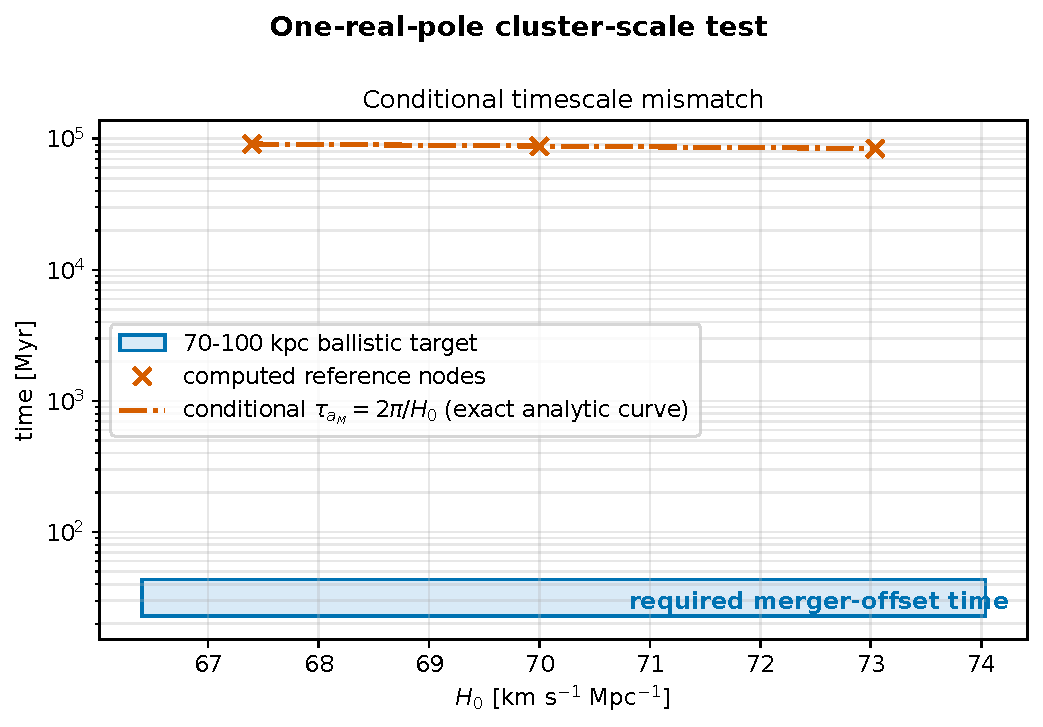
\includegraphics[width=\textwidth,height=0.64\textheight,keepaspectratio]{figures/r153/line_semantics/one_real_pole_exact_curve_r153.pdf}
\caption{Restricted transport-scale audit under the joint assumptions of one
constant real Debye pole, $\tau_{\rm pole}=\tau_{a_M}^{\rm match}=2\pi/H_0$,
and ballistic propagation $\ell=v\tau_{\rm pole}$.  The resulting
$201.96$--$269.28$~Mpc transport scale is compared with the declared
$70$--$100$~kpc merger-offset target, exposing a factor
$2.02\times10^3$--$3.85\times10^3$ mismatch.  This is a conditional
Level-A no-go inside those assumptions, not a constraint on multipole,
dispersive, non-ballistic, or separately owned causal response kernels.
The displayed line is the densely sampled exact analytic relation
$\tau_{\rm pole}=2\pi/H_0$; the three crosses are the frozen reference nodes.
Colour is redundant with line style, markers, luminance contrast and direct
labels.  The declared target interval is repeated by its luminance-separated
fill and both boundary lines, rather than by a decorative texture.  Complementary full-width panels are retained in Appendix~\ref{app:r129_visual_acoustic_cluster_gates}.}
\label{fig:r114_one_real_pole_cluster_scale_no_go}
\end{figure}

\paragraph{Solar-System closure.}
For every cosmologically interesting point, the same action must be solved
around an extended gravitating body with its cosmological boundary state.
The outputs are the scalar charge, metric coefficients, preferred-frame
terms and ephemeris observables.  The tested finite-body scalar mechanism has
\(\Xi_{\rm body}\ll1\) and supplies no mass screening for the named near-GR state.
Therefore strongly coupled scan points that fail the unscreened diagnostic in
Eq.~\eqref{eq:two_slope_unscreened_ppn_summary} need a different derived
response or metric completion; suppression may not be assumed.

\paragraph{Robustness axes.}
The minimum robustness programme varies, one axis at a time and jointly:
(i) ordering initial data; (ii) external-depth/lapse map; (iii) scalar
action coefficients; (iv) radiation and neutrino content; (v) matter and
photon metric assignments; (vi) recombination microphysics; (vii)
perturbation initial conditions; (viii) finite-body/environmental response;
and (ix) data calibration and covariance.  Each variation is rerun through
all downstream observables.  A point is not \emph{robust} when only its
background constraint remains small.

\paragraph{Completion and falsification protocol.}
For every observable the next accepted result must provide: (i) the varied
action and constrained physical fields; (ii) state and boundary data;
(iii) a stable background; (iv) the quadratic perturbation operators;
(v) the map to matter and photon observables; (vi) a frozen likelihood or
forward model; and (vii) counterexamples and limiting tests.  Failure of one
completion falsifies that completion, not unconnected ECT sectors.  Conversely,
agreement obtained by separately tuned operators is not evidence for one
unified ECT mechanism.

\subsection{Cosmological status map: conditional outputs, benchmarks, and Open targets}
\label{sec:mp_cosmo_predictions}
% ============================================================

The preceding subsections analysed a range of cosmological statements at
different derivation levels.
The purpose of the present subsection is to collect them in a single
summary table, analogous to the gravitational-sector summary in
\S\ref{sec:mp_grav_predictions}, and to distinguish explicitly
between strictly derived results, structural closure-level consequences,
and illustrative benchmark outcomes.

\begin{longtable}{@{}L{4.0cm}L{2.0cm}L{8.2cm}@{}}
\caption{Status map for the ordered-branch cosmology programme.}
\label{tab:cosmo_status_map}\\
\toprule
Claim & Status & Comment \\
\midrule
\endfirsthead
\multicolumn{3}{l}{\textit{Table~\ref{tab:cosmo_status_map} continued}}\\
\toprule
Claim & Status & Comment \\
\midrule
\endhead
\midrule
\multicolumn{3}{r}{\textit{Continued on next page}}\\
\endfoot
\bottomrule
\endlastfoot
Late-time acceleration in a supplied scalar completion
& Open / conditional
& A chosen positive potential can parametrise acceleration (proof-of-class);
  the ECT source, state and globally regular solution are Open \\
Bare scalar-ratio inequality $w_\phi^{\rm bare}\ge -1$
& A inside supplied stress / ECT Open
& Dimensionally normalised algebra only; $\dot F,\ddot F$ leave observable
  $w_{\rm eff}$ unconstrained \\
Conditional frozen-scalar Einstein--Friedmann consistency form
& A algebra inside supplied action / ECT Open
& Identification with calibrated $\Lambda$CDM is Level~C and requires
  $F_0,U_0,\rho_{m0},\rho_{r0}$, physical metric and state; reachability Open \\
ECT Hubble inference
& Open
& Sign and magnitude require one action-owned recombination-to-distance-ladder likelihood \\
JWST abundance and morphology
& Open
& Require one background, perturbation, halo, baryonic and survey-selection forward model \\
Cross-channel cosmological consistency
& Open
& Age, distance, growth and potential evolution become correlated only after one action and state derive them \\
Ordered-branch late-time-source route
& Open / conditional
& Scalar proof-of-class only; no derived ECT source or exclusion of an
  independent component \\
Background-to-galactic correlation hypothesis
& Open
& $a_{M,\rm bg}=c_{\rm char}H/(2\pi)$ is an auxiliary background proxy;
  no map to fitted $a_{M,\rm eff}$ is derived \\
Physical late-time-source history $w(a)$ from ECT
& Open
& Requires solved background, metric, state and joint likelihood \\
Primordial observables $(A_s,n_s,r)$ from ECT
& Open
& Not yet obtained from first principles in the present ECT cosmology
  programme \\
\end{longtable}

It is especially important to separate:
(i)~sign-level and closure-level structural consequences of the ordered
branch,
(ii)~benchmark numerical outcomes obtained within a specific
$\phi$-first truncation,
and (iii)~genuinely open cosmological targets that still require a
solved background history, perturbation closure, or full data fit.
This subsection should be read as a claim-by-claim status
inventory; the chapter-level synthesis of what is established, what is
closure-dependent, and what remains open is deferred to
Section~\ref{sec:mp_cosmo_status}.
Quantities not yet derived from ECT---such as an ECT-native formula
for $n_s$, a physical late-time-source history $w(a)$, or a
first-principles baryogenesis asymmetry---are not listed below as ECT
predictions.

\renewcommand{\arraystretch}{1.25}
{\small
\begin{longtable}{@{}L{0.20\textwidth}L{0.21\textwidth}L{0.15\textwidth}L{0.08\textwidth}L{0.25\textwidth}@{}}
\caption{Status-separated cosmological statements, conditional consequences,
and Open targets.}\label{tab:cosmo_predictions_summary}\\
\hline\hline
Statement / consequence & Formula / current disposition & Level & Section
  & Observational context \\
\hline
\endfirsthead
\hline\hline
Statement (cont.) & Current disposition & Level & Sec. & Obs.\ context \\
\hline
\endhead
\hline
\endfoot
\hline\hline
\endlastfoot

Spatial-flatness branch
  & $k=0$ only after the physical metric/embedding is supplied
  & B / Open
  & \S\ref{sec:flatness_ect}
  & topology is structural; cosmological metric ownership Open \\

Supplied-target monopole classification
  & $\pi_2(S^3)=0$ for the supplied orientation target
  & A-math conditional / physical Open
  & \S\ref{sec:relic_ect}
  & complete physical vacuum/configuration target and production history
    remain Open \\

Scalar-only perturbation inventory
  & one longitudinal scalar coordinate in the stated constrained map
  & A in map / physical Open
  & \S\ref{sec:mp_primordial}
  & complete perturbation action and metric map Open \\

No isocurvature in the scalar-only truncation
  & conditional on that one-mode inventory
  & B / physical Open
  & \S\ref{sec:mp_primordial}
  & orientation/matter entropy modes not yet classified \\

Physical tensor propagation
  & scalar characteristic cone does not determine it
  & Open
  & \S\ref{sec:mp_primordial}
  & tensor action, source, speed and damping missing \\

Macrocoherent branch minimum
  & $S_{\rm ord}=0$ iff $n_A=\mathrm{const}$ in a connected,
    constant-compatible admissible class
  & A-math in supplied model / ECT Open
  & \S\ref{sec:horizon_ect_main}
  & boundary/topological class and physical branch selection remain Open \\

Conditional physical-time completion
  & P4 supplies a direction; $\beta(\beta-\alpha)<0$ classifies a scalar operator;
    clock/lapse and chronology remain Open
  & A-math conditional / Open
  & \S\ref{sec:pre_lorentzian}
  & no physical-time theorem from ordering alone \\

Conditional bare scalar-ratio lemma
  & $w_\phi^{\rm bare}\ge -1$ if $\omega>0$ and
    $K_\phi^{\rm phys}+U>0$
  & A in supplied stress / ECT Open
  & \S\ref{sec:mp_flrw}
  & non-minimal terms leave physical $w_{\rm eff}(a)$ unconstrained \\

Ordered-branch age
  & $t_0=\int_{a_{\rm ord}}^1 da/(aH)$
  & A kinematics / owners Open
  & \S\ref{sec:universe_age}
  & supplied-completion estimate exists; physical map and microscopic completion Open \\

Correlated observables
  & $t_0$, $t_U$, $t_{\rm gal}$, $D_L$ from one $H(z)$
  & B struct.
  & \S\ref{sec:universe_age}
  & age / distance / JWST \\

ECT Hubble inference
  & sign and magnitude not identified without the full early+late pipeline
  & Open
  & \S\ref{sec:ect_cosmology_closure}
  & CMB, BAO, ladder and sirens \\

Cross-channel consistency
  & one future action and state must jointly generate $w(a)$, $H(a)$ and observables
  & Open
  & \S\ref{sec:ect_cosmology_closure}
  & joint background/perturbation fits \\

BBN consistency
  & accepted background must pass an ECT-native BBN/recombination pipeline
  & Open requirement
  & \S\ref{sec:ect_cosmology_closure}
  & no predicted saturation or drift history \\

Ordering-to-background stages
  & solver partition, not a predicted trajectory
  & Open scenario
  & \S\ref{sec:condensate_cosmo_evolution}
  & continuous exact-action evolution required \\

Candidate out-of-equilibrium ordering-transition route
  & missing-owner scenario; P4 supplies no real-time transition or state
  & C/Open
  & \S\ref{sec:mp_baryogenesis}
  & no jointly owned Sakharov completion, transport or washout \\

ECT background, age, Hubble and early-object closure
  & one supplied two-slope state gives conditional $H(z)$, distances, $\tau_{2s}$ and high-$z$ clocks; the physical map and microscopic completion remain Open
  & B/C/Open
  & \S\ref{sec:two_slope_background_proof_class}, \S\ref{sec:ect_cosmology_closure}
  & full perturbation, recombination, abundance and local-gravity pipeline required \\

Orientation determinant identity
  & $\det(\beta I-\alpha nn^{\mathsf T})=\beta^3(\beta-\alpha)$ at fixed
    amplitude and coefficients
  & A (algebra only)
  & \S\ref{sec:cc_problem}
  & does not derive a trace-free metric action or vacuum decoupling \\

Conditional trace-free shift covariance
  & $V\to V+C_0$, $C_I\to C_I-C_0$ leaves the explicitly supplied
    constrained scalar--tensor equations invariant
  & A inside named completion; ECT descent B/Open
  & \S\ref{subsec:unimodular_cc}
  & $C_I$ is an allowed global state/boundary datum \\

Two-slope late-background proof of class
  & a coercive ordinary scalar--tensor potential gives one stable de-Sitter
    root and a regular calibrated history, but is not shift invariant
  & A inside named action; benchmark C; ECT map Open
  & \S\ref{subsec:frw_cc}
  & no claim that the microscopic vacuum offset decouples \\

Conditional bare scalar-stress ratio
  & $w_\phi^{\rm bare}=(K_\phi^{\rm phys}-U)/
    (K_\phi^{\rm phys}+U)\ge-1$ under the stated sign conditions
  & A in supplied stress / ECT Open
  & \S\ref{sec:mp_flrw}
  & $F$-derivative terms determine the physical late-time expansion \\

Pseudo-Goldstone late-source route
  & Physical soft-mode operator, mass, state and abundance not identified
  & Open
  & \S\ref{subsec:goldstone_cc}
  & a C/Open Hubble-frequency orientation benchmark is retained; no
    late-source identification or numerical infrared-density scaling \\
\end{longtable}
}

\paragraph{What is explicitly not yet predicted.}
The present ECT cosmological programme does \emph{not} yet provide:
(i)~an ECT-native formula for the scalar spectral index $n_s$ or the
tensor-to-scalar ratio $r$;
(ii)~a physical late-time-source history $w(a)$;
(iii)~a first-principles derivation of the baryon asymmetry $\eta_B$.
These remain open tasks identified earlier in
\S\S\ref{sec:mp_primordial}, \ref{sec:mp_flrw}, and
\ref{sec:mp_baryogenesis}.

\paragraph{Status summary.}
The strongest current cosmological statements are conditional and structural,
not ECT-native numerical predictions:
a conditional planar spatial-flatness proof-of-class, the supplied-target
$\pi_2(S^3)=0$ classification, the constrained longitudinal scalar-coordinate
inventory, and the conditional positive-kinetic scalar-stress lemma.
The ordered-branch age definition is exact kinematics after its owners
are supplied.  One named two-slope action/state has active conditional
age, $H(z)$, distance, sound-horizon and high-redshift clock benchmarks.
Microscopic selection of the two-slope completion and the physical
metric/clock/front map remain Open, as do full Hubble inference and JWST
abundance or morphology.
A fully ECT-native perturbation spectrum and a first-principles
baryogenesis model remain central open problems.
A chapter-level synthesis of these statuses is given in
\S\ref{sec:mp_cosmo_status}.

% ============================================================
\subsection{Cosmological evolution: ECT vs.\ \texorpdfstring{$\Lambda$}{Lambda}CDM}
\label{sec:cosmo_evolution_comparison}
% ============================================================

\paragraph{Cosmological visualisations.}
A universal formation-to-present P1--P6 history remains Open.  The named
two-slope completion nevertheless supplies one reproducible post-ordering
conditional chronology, so it is displayed with its action/state,
dimensional-calibration and observable-map qualifications.  It must not be
read as a derived ordering transition, a universal age prediction, a Hubble
tension solution or a JWST abundance calculation.

\begin{figure}[!htbp]
  \centering
  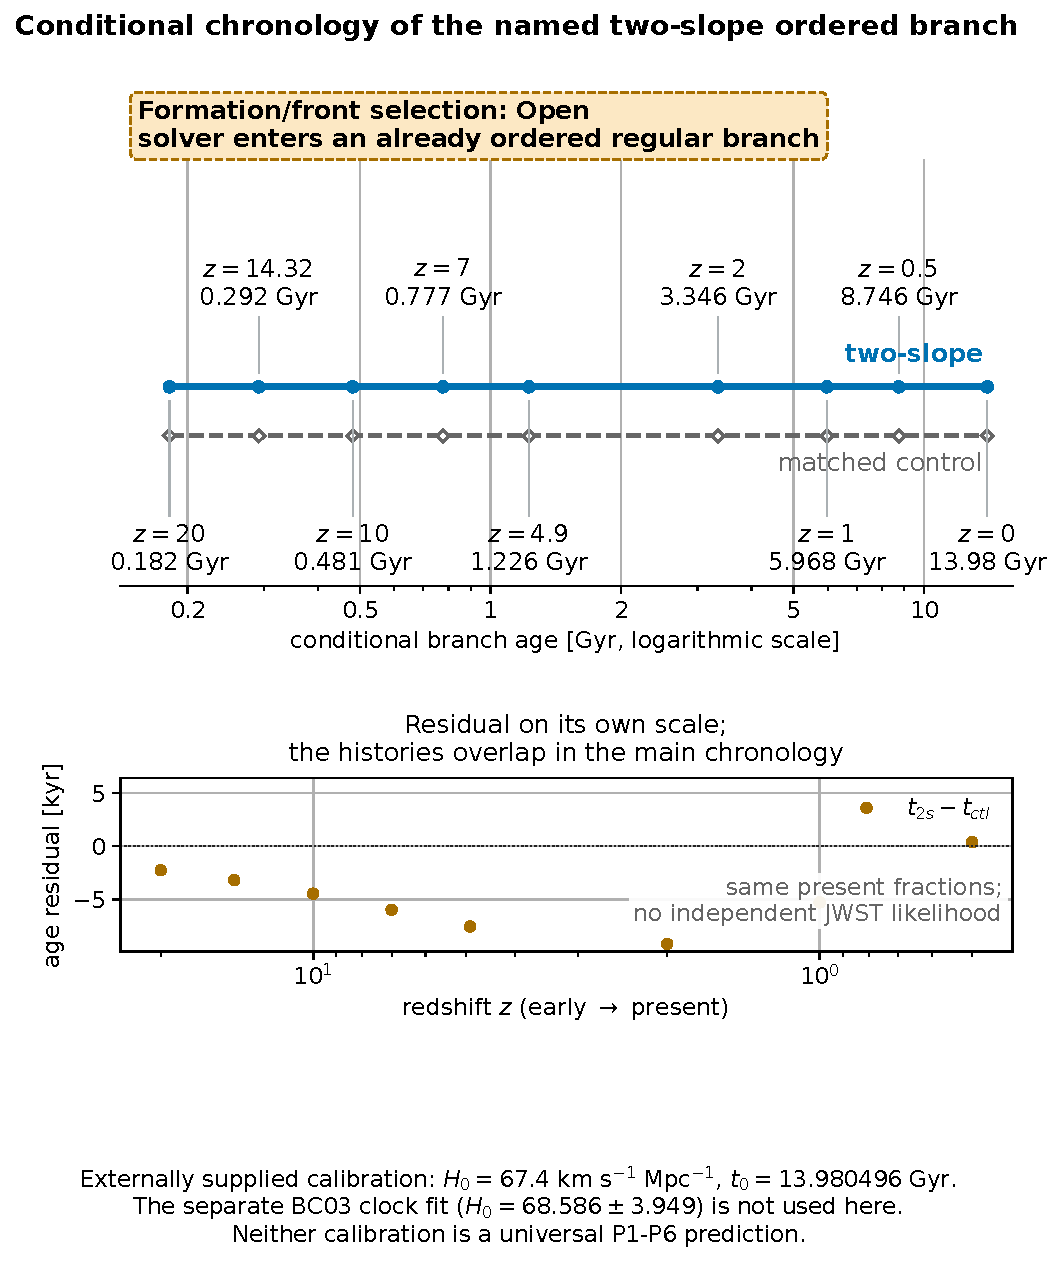
\includegraphics[width=\textwidth,height=0.66\textheight,keepaspectratio]{figures/r153/line_semantics/conditional_chronology_nodes_r153.pdf}
  \caption{\textbf{Conditional chronology of the named two-slope ordered
  branch.}
  The main track uses the externally supplied reference dimensional
  calibration $H_0=67.4\,\mathrm{km\,s^{-1}\,Mpc^{-1}}$, giving
  $t(z=10)=0.4814276482\,\mathrm{Gyr}$ and
  $t_0=13.9804960874\,\mathrm{Gyr}$.  The two-slope and matched-control
  histories nearly overlap; their difference is therefore shown separately
  in kyr.  The distinct BC03 clock fit
  $H_0=68.586\pm3.949\,\mathrm{km\,s^{-1}\,Mpc^{-1}}$ would give a different
  dimensional reading of the same orbit and is not mixed into this panel.
  Event ages share one externally supplied reference dimensional
  calibration and are not independent measurements or universal
  P1--P6 predictions.  Formation-front selection, BBN/recombination
  microphysics and the physical metric/clock map remain Open.  The figure is
  neither a universal P1--P6 age prediction, a Hubble-tension solution nor a
  JWST abundance calculation.  The residual panel shows nine evaluated event
  redshifts as unconnected markers; no intermediate residual interpolation is
  implied.}
  \label{fig:r123_conditional_universe_timeline}
\end{figure}

Table~\ref{tab:cosmo_vs_lcdm} summarises the key differences between
the standard $\Lambda$CDM picture and the ECT picture at each
cosmological epoch.
This comparison reflects the current status of the theory: exact
kinematic identities, conditional scalar equations and one globally regular
supplied two-slope $H(a)$ orbit are available, but P1--P6 do not select that
action/state and no owner-complete observable pipeline has yet been derived.
The early-Universe ordering layer likewise remains a structural scenario
rather than a completed first-principles nonequilibrium derivation.
The horizon problem can be reformulated in ECT as a branch-coherence
question.  A uniform map is the exact minimum of a separately supplied
positive sigma-model functional (Section~\ref{sec:horizon_ect_main}), but
P1--P6 do not yet derive that functional, the selected state, the required
coherence scale, or the primordial transfer.  This is therefore a
conditional route rather than a solution; an inflation-like ordering epoch,
if retained, is likewise only a conditional effective scenario.

\begin{longtable}{@{}L{0.20\textwidth}L{0.37\textwidth}L{0.37\textwidth}@{}}
\caption{Cosmological evolution: ECT vs.\ $\Lambda$CDM.} \\
\label{tab:cosmo_vs_lcdm} \\[-6pt]
\toprule
Epoch & $\Lambda$CDM & ECT \\
\midrule
\endfirsthead
\toprule
Epoch & $\Lambda$CDM & ECT \\
\midrule
\endhead
\midrule\multicolumn{3}{r}{\small\textit{(continued on next page)}}\\
\endfoot
\bottomrule
\endlastfoot
Pre-Planckian & Undefined; initial singularity at $t=0$ marks the
  boundary of the theory & Pre-Lorentzian Euclidean condensate regime
  (Level~B scenario); $O(4)$ symmetry unbroken,
  no Lorentzian metric is yet established,
  and no macroscopic time coordinate is available \\
Phase transition & Not present & P4 supplies a nonzero vector with $O(3)$
  stabiliser; physical $O(4)\to O(3)$ SSB remains Open.  The supplied scalar
  principal operator admits a Lorentzian characteristic representative on
  the declared coefficient component.  A physical clock/matter metric and
  nonequilibrium ordering history remain Open \\
Inflation & Separate inflaton field with ad-hoc potential &
  Possible inflation-like effective description of the ordering
  transition (Level~B structural scenario; no derived ECT
  horizon-resolution mechanism is presently available;
  see Section~\ref{sec:horizon_ect_main});
  ECT-native derivation of the primordial spectrum remains open
  (see \S\ref{sec:mp_primordial});
  not yet a full first-principles replacement for inflation \\
Flatness problem & Separate inflationary mechanism usually invoked to
  suppress $|\Omega_K|$ dynamically; in its absence, extreme fine-tuning
  of initial conditions is typically required &
  P1 supplies a flat Euclidean ambient metric.  A planar induced-metric
  completion has $k=0$ exactly, but the physical FLRW metric/embedding
  is not yet derived (Level~B/Open; see
  Section~\ref{sec:flatness_ect}) \\

Relic / monopole problem & Requires dynamical dilution mechanism
  (inflation) to dilute overproduced GUT monopoles and topological
  relics from the hot early Universe &
  The supplied $S^3$ orientation target has $\pi_2=0$, but physical-vacuum
  identification, transition and relic abundance are Open.  A hot GUT
  history is not postulated, but its absence is not derived; EW and
  later-sector relics require further development
  (see Section~\ref{sec:relic_ect}) \\
Primordial perturbations & Observed CMB spectrum:
  $n_s=0.9649\pm0.0042$~\cite{Planck2018},
  $r_{0.05}<0.036$ at 95\%~C.L.~\cite{BICEP2021};
  standard framework: inflaton slow-roll &
  One scalar coordinate in the strict map~(Level~A kinematics); one physical
  scalar mode is Level~B in the supplied reduced EFT; an ECT-native derivation
  of $n_s$, $r$ remains open~(OP3) \\
Reheating / radiation & Standard; inflaton decays into SM fields &
  A completed ordered branch must transfer energy from condensate excitations
  to the physical radiation bath; charged-spectrum population, efficiency and
  thermal completion remain Open~(OP3.3) \\
Matter domination & Cold dark matter particles & Cosmological matter
  content and matching Open; no ECT replacement for the cold component is
  derived.  Candidate condensate or particle sectors have uncomputed
  abundance and stability \\
Late-time acceleration & Cosmological constant $\Lambda=\text{const}$ &
  A regular two-slope scalar--tensor proof of class and a conditional scalar
  stress exist; the ECT action, state, metric and physical history are Open \\
Galactic scales & Dark matter halo in the standard interpretation &
  HRC-0/HRC-3 are augmented-model candidates with recomputed algebraic
  diagnostics; scalar-to-gravity matching, the field-level likelihood and any
  environment law remain Open \\
Origin of cosmic time & Lorentzian time fundamental from Big Bang
  onward & A relational Lorentzian-clock candidate is available only on the
  ordered branch; the physical clock/matter-metric bridge remains Open \\
Perturbation field content & Model-dependent; often single inflaton +
  tensor sector & One longitudinal scalar coordinate occurs in the stated
  constrained linear map; its physical projector and the tensor field,
  source, cone and
  tensor-to-scalar ratio remain Open~(\S\ref{sec:mp_primordial}) \\
Cosmic age interpretation & Time since Big-Bang singularity
  ($13.8$\,Gyr) & Duration of Lorentzian ordered branch;
  conceptually different quantity~(\S\ref{sec:universe_age}) \\
Hubble tension & Discrepancy between early- and late-inferred $H_0$ &
  No ECT sign or magnitude is identified; requires one recombination,
  distance and likelihood pipeline~(\S\ref{sec:ect_cosmology_closure}) \\
JWST early galaxies & Requires unusually rapid early assembly or revised
  forward modelling & ECT abundance and morphology are Open until the
  background, perturbation, halo, baryonic and selection owners are solved \\
Age--distance--Hubble--JWST relation & Often analysed as partly
  separate tensions & These channels must be generated by one future action
  and state; no common ECT mechanism is presently derived \\
Far future of the named models &
  Flat positive-$\Lambda$ $\Lambda$CDM tends to de~Sitter expansion &
  The supplied two-slope action tends to its stable root
  $\sigma\to\sigma_0$ and is future-regular (Level~A only inside that
  action/state; P1--P6 selection and the physical map remain Open) \\
Alternative future completion & A phantom completion can produce a Big Rip &
  Recollapse is an Open acceptance case for a different explicitly supplied
  action/state; it is not produced by the named two-slope orbit and no ECT
  timescale has been derived~(OP3) \\

\end{longtable}

\paragraph{Pre-Lorentzian regime.}
The pre-ordered / pre-Lorentzian regime, its structural status
(Level~A for configuration-space existence; Level~B for cosmological
realisation), and its conceptual consequences are developed in
\S\ref{sec:pre_lorentzian}; the branch-coherent reformulation of the
horizon problem is given in \S\ref{sec:horizon_ect_main}.

\paragraph{Condensate evolution and future branches.}
Ordering, a regular post-ordering background and any later evolution form a
solver and acceptance partition, not a universal three-stage trajectory.
The named two-slope action supplies only one regular post-ordering branch
ending at its stable de~Sitter root.  Formation/front dynamics and any
alternative recollapse branch require a different complete action/state and
remain Open.  Observable drift bounds and the physical expansion history are
acceptance tests of any completed branch.

\paragraph{Dimensionally separated scale inventory.}
The energy/matching pair $(\phi_0,v_2)$ and the conditional HRC matching length
$L_{\rm gal}$ have different dimensions and status.  No common hierarchy,
RG cascade, or background-to-galactic scale map is derived.

\paragraph{Distinctive structural features of the ECT cosmological
picture.}
Beyond the epoch-by-epoch comparison recorded in the table, several
broader distinctions separate ECT from $\Lambda$CDM.
The Euclidean construction supplies a pre-ordered configuration-space
regime and a scalar Lorentzian characteristic representative on the
ordered branch.  A physical cosmological clock/metric, globally regular
background, late-time source and the distance/Hubble/JWST observables are
not established consequences of that structure.  Their possible common
ownership by one condensate is the programme tested by the action and
observable gates of Appendix~\ref{app:ect_cosmology_observable_protocols},
not a present Level~B cosmological mechanism.

\paragraph{Internal versus comparative visualisations.}
\S\ref{sec:ect_cosmology_closure} and
Appendix~\ref{app:ect_cosmology_observable_protocols} are owner and
acceptance maps.  Figures~\ref{fig:r123_internal_external_history_map},
\ref{fig:r123_condensate_orbit} and
\ref{fig:r123_conditional_universe_timeline} now complement them with the
external/internal map, conditional post-ordering orbit and direct numerical
age comparison of the named supplied completion.  They do not replace the
missing formation, metric, perturbation and likelihood owners.

\paragraph{What is established and what remains open.}
The comparison above defines a common ECT calculation programme for
flatness/relic questions, the ordered-branch clock, Hubble inference and
early-object observables.  It does not establish a dynamical link among
those channels.  The strongest current statements concern the declared
configuration-space topology and the scalar characteristic operator;
their promotion to physical cosmology requires the missing metric, state
and perturbation owners.
P1--P6 selection of the late-time background, full Hubble inference and the
JWST forward model are Open.  The named two-slope action/state does supply a
conditional numerical age and background orbit, but not their microscopic
selection or an owner-complete observational likelihood.
What remains open is a fully ECT-native perturbation spectrum
(in particular $n_s$ and $r$), the quantitative nonequilibrium dynamics
of the ordering transition, and fully nonlinear structure formation.
The epoch-by-epoch comparison above should be read together with the
status synthesis of \S\ref{sec:mp_cosmo_status}.


% ============================================================
\subsection{Universe size, boundary, and force-law effective dimensionality}
\label{sec:universe_size}
\label{sec:mp_universe_size}
% ============================================================

\textit{Status: mixed.
The finite-domain / boundary discussion is a Level~B cosmological scenario
for a possible large-scale completion of the ordered branch.  The force-law
dimensionality below is instead point-source algebra inside the conditional HRC-0 point-source response after the identity bridge, distinct from the full HRC field problem
and not an action-derived ECT prediction.}
The first part of this subsection concerns the speculative cosmological
completion; the second records a conditional HRC-0 point-source diagnostic.  Its
formula follows only after the declared identity bridge and source profile are supplied.

\paragraph{Size of the ECT domain.}

In one possible ECT macroscopic completion~(Level~B), the observable
universe is a finite ordered Lorentzian domain in which the macroscopic
geometric branch is active. Beyond the causal boundary of this domain
the ordered-branch description itself ceases to remain reliable.
As the ordered amplitude weakens toward the edge of a finite domain,
the Lorentzian branch description is expected to break down and the
pre-ordered / pre-Lorentzian condensate regime to take over~(Level~B scenario;
explicit dynamics requires OP3).
This should be understood not as reaching a physical wall, but as
entering a regime in which the macroscopic geometric branch is no
longer a valid effective description.

No action-owned boundary solution or observable map fixes a finite-domain
size, and no inequality relating $R_{\rm domain}$ to $c/H_0$ follows from the
present framework.  The domain size remains Open.

This finite-domain scenario should not be read as fixing the late-time
background trajectory or the cosmological closure coefficients by
itself. It supplies a possible global support and boundary context for
the ordered branch. The observable FLRW quantities remain interior
relational variables of that branch and must ultimately be obtained
consistently with the same Euclidean ordered-domain realisation.

\paragraph{From domain scenario to measurable force-law response.}
The finite-domain discussion above concerns a speculative large-scale
completion of the ordered branch.
The force-law dimensionality below is exact Level-A algebra inside the
supplied HRC-0 point-source relation.  Its identity/source bridge is
Level-B/Open and its synthetic or data application is Level-C.  It is
independent of the finite-domain scenario and distinct from the full HRC field problem.

\paragraph{Topological versus force-law dimensionality.}
Two distinct notions of dimensionality appear in ECT.
The first is the topological dimensionality of the underlying arena,
which is postulated in~P1 (see \S\ref{sec:postulates} for why $d=4$ is
special).
The second is the effective force-law dimensionality extracted from the
radial scaling of the observed gravitational response.
These notions are different:
the arena remains topologically four-dimensional, while the diagnostic
computed inside the supplied HRC-0 point-source relation after a
separately declared B/Open gravity bridge moves
away from its near-Newtonian value in the imposed low-acceleration regime.
This conditional point-source response is not the full HRC field problem.
This does not mean that matter distributions become literally
two-dimensional; it refers only to the scaling of the effective
gravitational law.

\paragraph{Effective dimensionality at different scales.}

The conditional HRC-0 point-source relation supplies a scale-dependent
force-law diagnostic.  This does not imply a change of topological dimension,
a property of the full HRC field problem, or a closure-independent
condensate prediction.

\begin{figure}[!htbp]
\centering
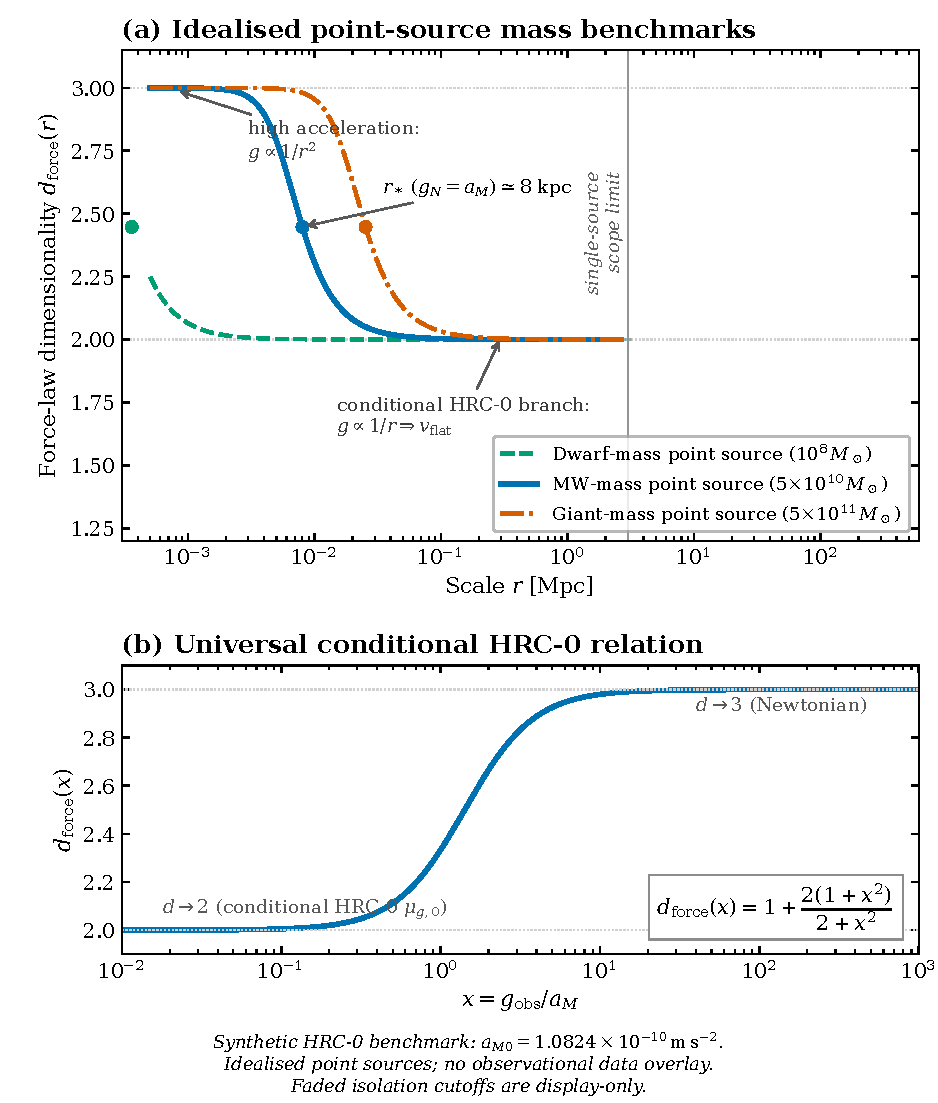
\includegraphics[width=0.95\textwidth]{figures/r149/fig_dimensionality_phi_typography_r149.pdf}
\caption{Point-source force-law diagnostic of the HRC-0 response
$\mu_{g,0}(x^2)=x/\sqrt{1+x^2}$.  The shape is Level-A algebra
inside the supplied augmented model; the identity/source bridge is
Level-B/Open and this synthetic figure is Level-C.  \textbf{(a)}~The three curves differ only by the
radial scale $r_*=\sqrt{G_NM/a_M}$ defined by $g_N=a_M$;
$r_*$ is not the $x=1$ radius, which is $2^{1/4}r_*$ here.  The imposed
point-source relation tends from $d_{\rm force}=3$ to $2$ and has
$d_{\rm force}(x=1)=7/3$.  \textbf{(b)}~The exact point-source collapse
$d_{\rm force}(x)=1+2(1+x^2)/(2+x^2)$.  Extended mass profiles instead
require their local $p_N(r)=-d\ln g_N/d\ln r$ in
Eq.~\eqref{eq:dforce_general}; no observed-galaxy markers are inferred.}
\label{fig:dimensionality}
\end{figure}

Figure~\ref{fig:dimensionality} separates the imposed point-source diagnostic
from the extended-profile generalisation developed below.

\paragraph{Force-law effective dimensionality.}

The conditional HRC-0 force-law diagnostic is defined by the local
acceleration exponent:
\begin{equation}
d_{\rm force}(r)
\;\equiv\; 1 - \frac{d\ln g_{\rm obs}}{d\ln r}\,.
\label{eq:dforce_def}
\end{equation}
In $d$ spatial dimensions the gravitational force scales as
$g \propto 1/r^{d-1}$; eq.~\eqref{eq:dforce_def} reads off
$d$ from the local force law.

\paragraph{Conditional one-variable collapse.}
After the supplied HRC-0 point-source relation and identity bridge are declared,
$d_{\rm force}$ is a function only of
$x=g_{\rm obs}/a_M$ for a point-mass source.  Its mass independence is
therefore algebra inside this one-variable closure.  It does not follow from
the ECT Universality Corollary and does not establish the gravity bridge, source map, or critical scale.

\paragraph{General formula.}
\textit{Status of the response function: the analysis uses the exact
HRC-0 shape $\mu_{g,0}(x^2)=x/\sqrt{1+x^2}$.  Its internal algebra
is Level~A in the augmented model; the identity/source bridge remains
Level~B/Open and the point-source application is Level~C.  The
calculation does not derive the bridge or $a_M$.  The limiting behaviour below is shared only by functions
for which the Newtonian and low-acceleration asymptotes are imposed.}

Starting from the conditional HRC-0 point-source relation
$\mu_{g,0}(x^2)g_{\rm obs}=g_N(r)$ with
$x\equiv g_{\rm obs}/a_M$, one obtains by logarithmic differentiation:
\begin{equation}
\boxed{
d_{\rm force}(r) = 1 + \frac{p_N(r)}
  {1 + \dfrac{d\ln\mu_{g,0}}{d\ln x}}\,,
}
\label{eq:dforce_general}
\end{equation}
where $p_N(r) \equiv -d\ln g_N/d\ln r$.
For a point mass $p_N = 2$.
The derivation is given in Appendix~\ref{app:deff_method}.

\paragraph{Closed-form result.}
For HRC-0, $\mu_{g,0}(x^2)=x/\sqrt{1+x^2}$, one finds
$d\ln\mu_{g,0}/d\ln x=1/(1+x^2)$, and therefore
\begin{equation}
\boxed{
d_{\rm force}(x)
=
1 + 2\,\frac{1+x^2}{2+x^2}
}
\label{eq:dforce_closed}
\end{equation}
for a point-mass Newtonian source $p_N=2$.
Thus:
\begin{itemize}
  \item in the high-acceleration Newtonian asymptote $x\gg1$:
    $d_{\rm force}\to 3$, corresponding to $g\propto 1/r^2$;
  \item in the imposed low-acceleration regime $x\ll1$:
    $d_{\rm force}\to 2$, corresponding to $g\propto 1/r$
    and asymptotically flat rotation curves;
  \item at the transition point $x=1$:
    $d_{\rm force}(1)=1+\tfrac{4}{3}=\tfrac{7}{3}\approx2.33$.
\end{itemize}

Thus the conditional HRC-0 point-source law yields a smooth diagnostic crossover from an effectively
three-dimensional Newtonian regime at large acceleration to an
effectively two-dimensional force-law regime at low acceleration.

\paragraph{Representative characteristic radii.}
Define
\[
r_*=\sqrt{\frac{G_N M}{a_M}}
\]
as the reference radius where $g_N=a_M$.  It is not the exact $x_g=1$
radius: $r_{x_g=1}=r_*/\sqrt{\mu_g(1)}$.  Thus HRC-0 gives
$r_{x_g=1}=2^{1/4}r_*$, while conditional HRC-3 gives
$r_{x_g=1}=\sqrt{3\sqrt2/2}\,r_*$.
The characteristic radius is set by the independently supplied $M$ and
$a_M$.  Because $a_M$ is fitted or
matched rather than derived, these radii are conditional coordinate outputs,
not ECT predictions or evidence for an observable transition.

\paragraph{Observational extraction and closure test.}
A data-level test would require independent profiles for
$g_{\rm obs}(r)$ and baryonic $g_N(r)$ together with the local
$p_N(r)$ in Eq.~\eqref{eq:dforce_general}.  The closed $p_N=2$ curve is a
synthetic point-source benchmark, not a universal extended-galaxy prediction.
No such observational extraction is performed here.

\paragraph{Status.}
The displayed point-source $d_{\rm force}(x)$ is Level-A algebra inside
the supplied HRC-0 response model.  The identity/source bridge is
Level-B/Open and the plotted application is Level-C.  It is not a theorem
about microscopic topology and does not derive a finite-domain boundary.

\paragraph{What is established and what remains open.}
The finite-domain interpretation is a Level-B cosmological scenario
whose large-scale completion remains Open (OP3).  Separately, the force-law formula is Level-A algebra inside the supplied HRC-0
response, Level-B/Open after the declared gravity/source bridge, and Level-C
when applied as a synthetic or data diagnostic.
What remains open is:
(i)~a first-principles derivation of any finite-domain boundary from
bare~P3;
(ii)~a full data-level extraction of $d_{\rm force}(x)$ from observed
rotation-curve samples;
(iii)~the extension of the force-law dimensionality concept beyond the
galactic branch to morphological or cosmic-web scales~(OP8).


% ============================================================
\subsection{What is established and what remains open}
\label{sec:mp_cosmo_status}
% ============================================================

\subsubsection*{Physical interpretation}

The present cosmological programme studies a possible large-scale history
built on the supplied ordered-gradient chart and its macroscopic background
variable~$\phi_b(z)$.  It explores the conditional interpretation that a
Lorentzian cosmological history begins only after a physical ordered state
has formed.  P4 itself does not establish such a state or transition.
A pre-ordered regime therefore motivates, but does not derive, a relational
start of the Lorentzian clock.  A stationary state and selection mechanism,
homogeneous FLRW solution, late-time source, numerical age, Hubble inference
and JWST forward model are separate owner-dependent targets until one
complete action and state derive them together.

This unified reading should not be overstated.
Some parts of the cosmological sector are already strict structural
results, while others remain closure-level consequences of the present
$\phi$-first macroscopic completion.
The purpose of the present subsection is therefore not to introduce new
cosmological claims, but to summarise which parts of the ECT
cosmological programme are already established, which are benchmarked,
and which remain open.
It should therefore be read as a status synthesis of the chapter rather
than as an additional derivational step.
A detailed claim-by-claim status table is given in
\S\ref{sec:mp_cosmo_predictions}.
The present synthesis instead groups the chapter by epistemic status
and by the role each result plays in the ordered-branch cosmological
programme.

\subsubsection*{Strictly established and status-separated}

\begin{enumerate}[label=(\roman*)]
  \item The programme compares a hypothetical pre-ordered Euclidean class with
    the ordered-gradient chart supplied by P4.  P4 itself neither owns the
    former class nor derives a transition between them.  Calling the former
    ``pre-Lorentzian'' is programme language; a realised physical Lorentzian
    branch, clock and chronology remain Open
    (\S\ref{sec:pre_lorentzian}).
  \item Spatial flatness $k=0$ is a property of the named baseline
    cosmological completion, not a consequence of P4 alone
    (\S\ref{sec:flatness_ect}).
  \item The supplied orientation target satisfies $\pi_2(S^3)=0$.
    Excluding a physical monopole class requires identifying it with the
    complete vacuum/configuration space; that step is Open
    (\S\ref{sec:relic_ect}).
  \item Scalar integrability leaves one longitudinal scalar coordinate in the
    strict map; one physical mode is conditional on the supplied linear EFT,
    domain and projector.  This does not exclude independent isocurvature
    modes in additional matter/completion sectors~(\S\ref{sec:mp_primordial}).
  \item For supplied $\beta(\beta-\alpha)<0$, the scalar principal tensor
    defines one scalar characteristic cone.  A physical tensor Hessian, metric, clock and
    $c_{\rm GW}$ remain Open completion gates~(\S\ref{sec:mp_primordial}).
  \item In a separately supplied positive sigma-model functional, a uniform
    orientation is its global minimum.  The ECT owner, state selection,
    coherence scale and cosmological transfer remain Open
    (\S\ref{sec:horizon_ect_main}).
\end{enumerate}

\subsubsection*{Structural closure-level results (Level~B)}

\begin{enumerate}[label=(\roman*)]
  \item The homogeneous FLRW branch of the $\phi$-first closure is
    well-defined and supplies the cosmological background
    equations~(\S\ref{sec:mp_flrw}).
  \item The supplied stress obeys the bare scalar-ratio identity
    $w_\phi^{\rm bare}\ge -1$ when $\omega(\phi)>0$ and
    $K_\phi^{\rm phys}+U>0$; this does not constrain the observable
    effective history~(\S\ref{sec:mp_flrw}).
  \item The age of the Universe is reinterpreted as the duration of the
    Lorentzian ordered branch rather than the elapsed time since a
    fundamental singularity~(\S\ref{sec:universe_age}).
  \item The quantities $t_0$, $t_U(z)$,
    $t_{\rm gal}(z_{\rm obs};\,z_{\rm form})$, and $D_L(z)$ are all
    controlled by the same ordered-branch background
    $H(z)$~(\S\ref{sec:universe_age}).
  \item One named ECT-compatible candidate completion now gives a derived conditional age and
    background distances after a declared state and dimensional calibration.
    Full Hubble inference and JWST abundance remain Open.  A completed
    cosmology must derive their physical maps and correlations from one
    action/state and one consistent calibration
    (\S\ref{sec:ect_cosmology_closure}).
  \item P4 supplies an ordered-gradient chart, but not the real-time transition
    history or nonequilibrium state required by Sakharov baryogenesis.
    The baryon current, violating vertex, CP coefficient, transport and
    washout owners remain Open~(\S\ref{sec:mp_baryogenesis}).
  \item The three named regimes---ordering, a regular post-ordering
    background and any later evolution---are a solver/acceptance partition,
    not a structural three-stage history.  The supplied two-slope action has
    one future-regular orbit; P1--P6 selection, the formation front and any
    alternative far-future branch remain Open
    (\S\ref{sec:condensate_cosmo_evolution}).
  \item The force-law dimensionality crossover
    $d_{\rm force}:3\to7/3\to2$ is conditional point-source algebra
    inside the conditional HRC-0 point-source diagnostic, not the full HRC field problem;
    data-level extraction remains Open~(\S\ref{sec:universe_size}).
\end{enumerate}

\subsubsection*{Current numerical status}

A named supplied two-slope action/state now has a globally regular
two-integrator orbit, the conditional value
$\tau_{2s}\equiv H_{2s}(0)\Delta t=0.96368678$, distances,
high-redshift clock budgets, an imported-recombination sound-horizon
diagnostic, restricted quasistatic growth, and restricted instantaneous
Weyl/derivative carriers.  None is a P1--P6-selected universal cosmology or a
full likelihood result.  The physical metric, ordering state, recombination,
gauge-complete perturbations and finite-body closure remain Open.  Every
further numerical result must use the exact solver protocol of
Appendix~\ref{app:late_cosmo_algorithm}.

\subsubsection*{What remains open}

\begin{enumerate}[label=(\roman*)]
  \item A fully ECT-native derivation of the primordial spectrum,
    in particular $n_s$, $A_s$, and
    $r$~(\S\ref{sec:mp_primordial}, OP3).
  \item The nonequilibrium microdynamics of the ordering transition
    from bare~P3.
  \item The microscopic origin of the effective closure functions,
    in particular $U(\phi)$ and the full background history
    $\phi_b(z)$~(OP3).
  \item A closure-independent late-time fit of the ECT background
    sector to the combined age / distance / Hubble / JWST data.
  \item A first-principles ECT derivation of the baryon asymmetry
    $\eta_B$; the present manuscript contains only an operator/state
    owner inventory, not an established Sakharov-compatible ECT
    environment or numerical benchmark~(\S\ref{sec:mp_baryogenesis}, OP7).
  \item A fully self-consistent high-redshift completion of the
    background ansatz compatible with BBN and with the late-time
    Hubble sector.
  \item Fully nonlinear structure-formation calculations
    (N-body / hydrodynamic level) for the JWST regime.
  \item A first-principles derivation of any finite ordered-domain
    boundary and of its relation to the pre-Lorentzian
    regime~(\S\ref{sec:universe_size}).
\end{enumerate}

\paragraph{Chapter-level synthesis.}
The strongest ECT cosmological results are structural rather than
numerical.
The architecture supplies a pre-ordered regime; P1 fixes ambient Euclidean
flatness, while $k=0$ requires the declared planar induced-metric completion.
The supplied $S^3$ orientation target has no $\pi_2$ class; the physical
vacuum/relic conclusion is Open.  The strict scalar map has one longitudinal
perturbation coordinate.  Ownership of
the physical FLRW metric and of a complete one-mode scalar perturbation sector
remains Level~B/Open.
The late-time cosmological sector is organised by explicit owners.  The
central gaps are a globally regular action-owned background, the ordering
clock, the gauge-reduced perturbation and photon/matter-metric sectors,
and the observable-specific forward models listed in
Appendix~\ref{app:ect_cosmology_observable_protocols}.


% ==============================================================
\section{Galactic and Astrophysical Phenomenology}
\label{sec:mp_galactic_phenom}
% ==============================================================

\paragraph{Scope and status of the galactic programme.}
This chapter keeps two constructions separate: S, the Level-B scalar
ansatz, and ERP-$\Phi$/HRC, the augmented-model response candidate with
its newly recomputed Level-C diagnostic pipeline.  The physical coordinate,
source/force/metric normalisation, body solution, screening and map from the
live action to HRC remain Open.

\paragraph{What is and is not claimed here.}
The HRC algebraic diagnostic addresses selected BTFR, RAR and
rotation-curve benchmarks without an explicit particle-halo term in that
fit model; it is not yet the nonspherical field-level calculation.  The exact local-response theorem proves that every strictly increasing
algebraic transform preserves the ordering and maxima of the supplied total
projected baryon proxy.  It therefore cannot itself displace the total-response
maximum, but may inherit gas/BCG separations already present in the input and
does not constrain residual-map extrema.  These are Level-C closure outputs, not first-principles
consequences of the corrected scalar equation.  Neither a signed environment
law nor Solar-System screening is inferred from the fits.

The scalar audit is documented in
Appendix~\ref{app:lof_full_derivation}; the conditional HRC gravity
functional and SPARC diagnostic registry in
Appendices~\ref{app:galactic_phi_closure} and
\ref{app:sparc_computation}; the cluster-merger owner protocol is in
Appendix~\ref{app:ect_cosmology_observable_protocols}.  Implementation algorithms are collected
in Appendix~\ref{app:algorithms}.

% ============================================================
\subsection{Scalar audit S and conditional HRC gravity functional G}
\label{sec:mp_galactic}
% ============================================================

\textit{Status: the amplitude coordinate and conditional scalar
identities belong to the Level-B scalar ansatz.  ERP-$\Phi$/HRC is a new
augmented-model constitutive candidate with the layered status stated in
Sec.~\ref{sec:hrc_erp_candidate}; its gravity ownership is Open.  The SPARC fit outputs and plotted curves below are HRC-only Level-C
algebraic diagnostics with a poor absolute held-out likelihood.  Their fitted $a_M$ values are not a derivation of the scale,
an environment law, or a field-level disk prediction.}

For the amplitude coordinate and conditional scalar-response identities,
see Appendix~\ref{app:lof_full_derivation} (Sections~AJ.1--AJ.4).  The conditional HRC gravity functional and its Open identity-bridge
ownership are documented below and in
Appendix~\ref{app:galactic_phi_closure}.

\subsubsection*{Amplitude coordinate of the separate scalar ansatz S}

The separate Level-B scalar ansatz S defines
\begin{equation}
  \phi\equiv\phi_u
  =\frac{1}{\beta_\phi}\ln\frac{u}{u_\infty},
  \qquad
  F(\phi)=\frac{u}{u_\infty}=e^{\beta_\phi\phi}.
  \label{eq:phi_amplitude_def}
\end{equation}
This is a definition of the $u$-based coordinate together with the Level~B
matching $f=\bar M_{\rm Pl}^2F$.  It is distinct from the exploratory
anisotropy coordinate $\psi_K=\ln(\Delta_K/\Delta_{K,{\rm vac}})$ used in
Appendix~\ref{app:lof_full_derivation}; no $u\leftrightarrow\Delta_K$ bridge has
been derived.  The particular functions $\omega(\phi)$ and $U(\phi)$ used in
phenomenological calculations are closure choices, not inherited
coefficients already fixed by bare~P3.

\paragraph{Scalar-only local response.}
For a coordinate-independent audit, write the scalar closure as
\[
S_q=\int\!d^4x\sqrt{-g}\left[
  \frac12f(q)R-\frac12K(q)(\partial q)^2-V(q)
\right]+S_m[g,\Psi],
\qquad a(q)\equiv\frac{d\ln f}{dq}.
\]
Eliminating the Ricci scalar between the scalar equation and the trace of
the metric equation gives, for non-relativistic matter
$T\simeq-\rho_{\rm m}$,
\begin{align}
  \mathcal A(q)\Box q
  +\mathcal C_X(q)(\partial q)^2
  -\mathcal E(q,\rho_{\rm m})&=0,
  \label{eq:phi_eom_local}\\
  \mathcal A(q)&=K(q)+\frac{3f_{,q}^2}{2f},\\
  \mathcal C_X(q)&=\frac12K_{,q}+\frac12aK
                  +\frac32a f_{,qq},\\
  \mathcal E(q,\rho_{\rm m})&=V_{,q}-2aV-\frac{a}{2}\rho_{\rm m}.
\end{align}
No universal $4\pi$ coefficient appears in this equation.  Factors of
$8\pi G_N$ enter only after a specified normalisation and division by
$f$; they cannot replace the non-minimal coupling derivative $f_{,q}$.

A homogeneous local root satisfies $\mathcal E(\bar q,\rho_{\rm m})=0$.
The derivative required by the implicit-function theorem is the partial
derivative at fixed Jordan-frame matter density,
\begin{align}
 \mathcal E_{,q}\big|_{\rho_{\rm m}}
 &=V_{,qq}-2a_{,q}V-2aV_{,q}
   -\frac{a_{,q}}{2}\rho_{\rm m},\\
 \mathcal E_{,q}\big|_{\mathcal E=0}
 &=V_{,qq}-\left(2V+\frac{\rho_{\rm m}}2\right)a_{,q}
   -a^2(4V+\rho_{\rm m}).
 \label{eq:local_response_Eq}
\end{align}
Let $f,K,V$ be sufficiently smooth, let $f>0$, take
$\rho_{\rm m}$ as an independently specified local Jordan-frame density, and
fix a regular scalar coordinate together with one boundary/state branch.
The implicit-function theorem requires
$\mathcal E(\bar q,\rho_{\rm m})=0$ and
$\mathcal E_{,q}(\bar q,\rho_{\rm m})\ne0$; it does not require a sign for
$\mathcal E_{,q}$.  It then gives
\begin{equation}
  \frac{d\bar q}{d\rho_{\rm m}}
  =\frac{a(\bar q)}{2\mathcal E_{,q}},
  \qquad
  \frac{d\ln \bar f}{d\rho_{\rm m}}
  =\frac{a(\bar q)^2}{2\mathcal E_{,q}}.
  \label{eq:local_response_monotonicity}
\end{equation}
On a stable-root branch with $\mathcal E_{,q}>0$ the second expression is
non-negative.  The separate condition $\mathcal A>0$ is a kinetic-stability
guard for the supplied local scalar equation, not a hypothesis used by the
implicit-function theorem.  The logarithmic response is invariant under a
smooth regular reparameterisation of $q$; the sign of
$d\bar q/d\rho_{\rm m}$ alone is coordinate dependent.

Two dimensionally explicit negative controls make the scope fail-closed.
Let $q$ be dimensionless, $f_\star>0$ carry mass dimension two,
$V_\star>0$ carry mass dimension four, and
$\widehat\rho\equiv\rho_{\rm m}/V_\star$.  First take
\[
 a(q)=q,\qquad f(q)=f_\star e^{q^2/2},\qquad
 V(q)=V_\star\!\left[\frac14+(q-1)+\frac54(q-1)^2\right].
\]
At $(q,\widehat\rho)=(1,1)$, $\mathcal E/V_\star=0$ and the full
fixed-density derivative is
$\mathcal E_{,q}/V_\star=-1/2$, whereas deleting the $a_{,q}$ terms gives
the opposite sign, $+1/2$.  Thus those terms can reverse the root-curvature verdict even when
the independently supplied kinetic guard is healthy.  Second, take
\[
 \mathcal E=V_\star\left(q-q^2-\frac{\widehat\rho}{2}\right).
\]
The point $(q,\widehat\rho)=(1/2,1/2)$ has
$\mathcal E=\mathcal E_{,q}=0$, while the lower branch
$q_-=[1-\sqrt{1-2\widehat\rho}]/2$ has divergent susceptibility as
$\widehat\rho\to(1/2)^-$.  Division by $\mathcal E_{,q}$ is therefore
forbidden at the fold; no continuation, screening law or finite-body charge
is inferred there.  For relativistic matter the full trace $T$ replaces
$-\rho_{\rm m}$; scalar-dependent matter masses or correlated matter--scalar
initial data also alter the differentiation.  This is Level~A conditional
local mathematics inside the supplied closure.  It establishes neither a
finite-body charge, density-growing response mass, screening law, PPN limit,
nor the earlier $4\pi$, $a_M$ or $\Xi$ formulae.

\paragraph{Derived origin versus benchmark closure.}
The amplitude coordinate is a variable of the supplied ordered-chart EFT;
existence of a physical ordered branch does not follow from that
parametrisation.  The identifications
$f/\bar M_{\rm Pl}^2=u/u_\infty$, the functions $K,V$, their connection to
the soft anisotropy sector, and the HRC response used in the algebraic SPARC diagnostic are separate
matching inputs.  The HRC response algebra is Level~A inside the supplied augmented
model.  Its identity/microscopic gravity bridge is Level~B/Open, whereas the
galaxy fits are Level~C; it is not a realisation of the separate scalar
ansatz until those bridges are derived.

\subsubsection*{What the bare condensate-amplitude test establishes}

For the supplied linear proxy equation, a compact source has an unsourced
exterior Yukawa tail of range $\sqrt{\beta}/m_\sigma$.  Therefore a proposed
range $L$ must satisfy the exact necessary condition
$m_\sigma/\sqrt{\beta}\lesssim L^{-1}$.  ECT presently supplies no owned map
from the P3 curvature to the physical proxy parameters, so this theorem does
not support a numerical galactic application.  It also does not forbid an
extended profile driven by an extended source; that response remains
unquantified until the source vertex is supplied.

If a light amplitude completion is proposed instead, Solar-System and
equivalence-principle tests constrain its canonically normalised matter
coupling and finite-body solution.  They do not imply an automatic
order-unity exclusion without those inputs.  The result therefore rejects
only the separately specified unscreened linear Brans--Dicke benchmark; the
radial-proxy branch supplies a symbolic range gate, not a numerical
exclusion.  It does not select
$\phi_u$ or derive the conditional HRC functional G; its algebra is A inside
the augmented model, its microscopic bridge is B/Open, and its data
applications are C.  Appendix~\ref{app:lof:branch1} records the recovered
exterior-tail theorem, while Fig.~\ref{fig:regime_diagram} displays the
remaining Open matching problem.

\begin{figure}[!htbp]
\centering
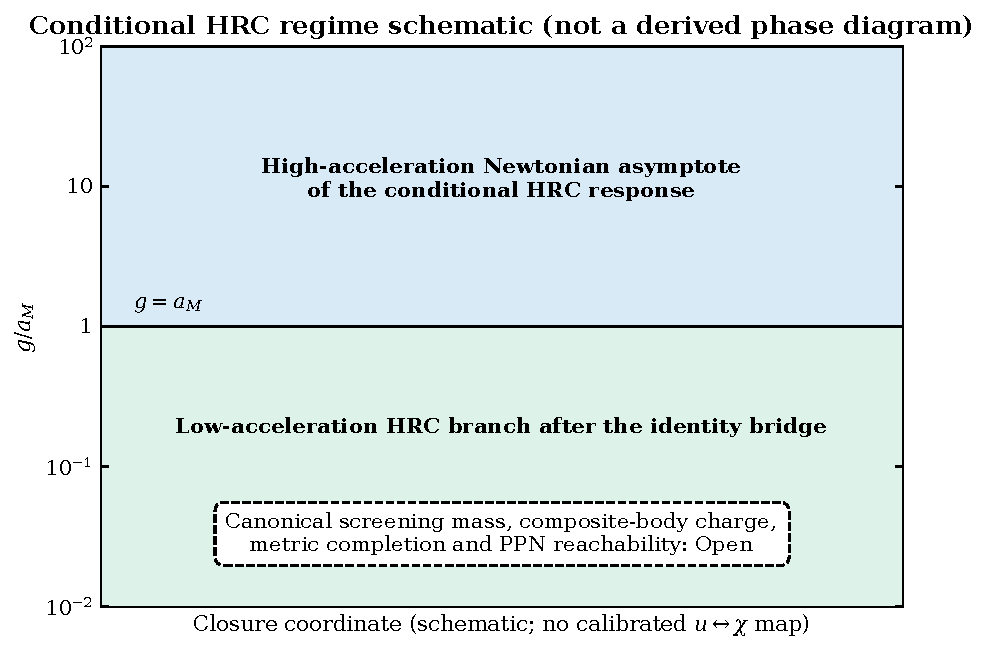
\includegraphics[width=0.82\textwidth]{figures/r149/fig_regime_diagram_typography_r149.pdf}
\caption{Status diagram for the galactic programme.  The vertical axis
shows only the two response regimes of the conditional HRC diagnostic.
The horizontal scalar-closure axis has no calibrated physical coordinate:
neither $u\leftrightarrow\Delta_K$ nor S$\to$G has been derived.  The Open gate
collects the required finite-body solution, scalar charge, screening trend,
PPN test, and galactic source/force normalisation.}
\label{fig:regime_diagram}
\end{figure}

%%% -----------------------------------------------------------
\subsubsection*{Local response mass and the open screening problem}
\label{subsec:lof_screening}

\textit{Status: the local linearisation below is derived inside the stated
scalar--tensor closure.  Density-enhanced screening, finite-body charges,
and compatibility with Solar-System bounds remain Open (OP-screen).}

Let $\bar q(\rho_{\rm m})$ be a stable homogeneous root of
$\mathcal E=0$.  Linearising
$q=\bar q+\delta q$ and neglecting background gradients gives
\begin{equation}
  \left(\nabla^2-m_{\rm loc}^2\right)\delta q
  =-\frac{a(\bar q)}{2\mathcal A(\bar q)}\,
    \delta\rho_{\rm m},
  \qquad
  m_{\rm loc}^2(\rho_{\rm m})
  =\frac{\mathcal E_{,q}(\bar q,\rho_{\rm m})}
         {\mathcal A(\bar q)}.
  \label{eq:mphi_main}
\end{equation}
For SI mass density $\rho$, $\rho_{\rm m}=c^2\rho$.  Positivity of
$\mathcal A$ and $\mathcal E_{,q}$ gives a locally stable Yukawa response.
Along a regular root, the exact total derivative is
\begin{equation}
 \frac{d m_{\rm loc}^2}{d\rho_{\rm m}}
 =\frac1{\mathcal A}
  \left[-\frac{a_{,q}}2
  +\frac{a\,\mathcal E_{,qq}}{2\mathcal E_{,q}}\right]
  -\frac{a\,\mathcal A_{,q}}{2\mathcal A^2},
 \label{eq:mphi_density_derivative}
\end{equation}
with all functions evaluated on that branch.  Its sign is unrestricted and
depends on the complete $f,K,V$ closure.  Therefore local stability does not
derive density-enhanced screening.

\paragraph{What a screening claim additionally requires.}
A viable screened branch must supply (i)~a specified closure for $f,K,V$;
(ii)~regular interior and exterior solutions for an extended source;
(iii)~the scalar charge and matching across the body; (iv)~the metric
potentials entering post-Newtonian observables; and (v)~a parameter region
satisfying laboratory, equivalence-principle, and Cassini constraints.
None of these follows from the positivity of $m_{\rm loc}^2$ alone.

\paragraph{Benchmark length scales.}
The local response length
$\lambda_{\rm loc}=m_{\rm loc}^{-1}$ is defined only where the assumptions
of Eq.~\eqref{eq:mphi_main} hold.  No calibrated sub-AU, kpc, or Mpc
hierarchy follows from the present $f,K,V$ system.  Numerical response
lengths require a specified closure and finite-body solution.
Appendix~\ref{app:screening_benchmarks} records the corresponding
response-length guards and finite-body owner checklist.

\paragraph{Relation to known screening paradigms.}
If a future solution yields a response mass increasing with ambient density,
its phenomenology would resemble chameleon screening
\cite{KhouryWeltman2004}.  At present this is an analogy, not a derived ECT
mechanism.  Symmetron and Vainshtein comparisons likewise require the
missing nonlinear action and body solutions
\cite{HinterbichlerKhoury2010,Vainshtein1972}.


%%% -----------------------------------------------------------
%%% -----------------------------------------------------------
\subsubsection*{Distinct length scales and their current status}
\label{subsec:lof_scales}

\textit{Status: the definitions are distinct; their numerical ordering in
the galactic closure is not presently derived.}

Four scales appear in different parts of the programme:
\begin{enumerate}[label=(\roman*)]
  \item \textbf{Microscopic condensate scale.}
  The homogeneous-P3 radial correlation length
  $\xi_{\rm P3}=m_{\Phi,\mathrm{rad}}^{-1}$ is microscopic under the declared
  Planck-scale calibration.  It is neither a P4 pole length nor the unresolved
  soft scalar coordinate used in galactic fits.

  \item \textbf{Local scalar response length.}
  Where Eq.~\eqref{eq:mphi_main} is applicable,
  $\lambda_{\rm loc}=m_{\rm loc}^{-1}$.  Its density dependence and its
  finite-body interpretation are Open.

  \item \textbf{Phenomenological transition radius.}
  The fitted acceleration $a_{M,\rm eff}$ defines
  $r_*=\sqrt{G_NM_{\rm bar}/a_{M,\rm eff}}$.  This is an algebraic
  scale of the HRC algebraic diagnostic, not yet a prediction of the scalar action.

  \item \textbf{Cosmological reference scale.}
  $H_0^{-1}$ is the cosmological length.  The numerical proximity of a
  fitted galactic acceleration to $cH_0/(2\pi)$ is a phenomenological
  matching observation; its ECT coefficient and dynamical origin remain
  open.
\end{enumerate}

The candidate ordering sometimes used for intuition is
\begin{equation}
  \label{eq:scale_hierarchy}
  \xi_{\rm P3}\ll\lambda_{\rm loc}\lesssim r_*\ll H_0^{-1}
  \qquad\text{(benchmark hypothesis, not a derived hierarchy).}
\end{equation}
It may be tested only after $m_{\rm loc}(\rho)$, the body charge, and the
map to $a_M$ are fixed.  Consequently this hierarchy cannot presently
be used to claim simultaneous derivation of Solar-System screening and
galactic critical dynamics.

\subsubsection*{Anisotropy-loop audit and the missing amplitude bridge}
\label{subsec:lof_oneloop}

\textit{Status: exact Gaussian-normalisation cancellation / derivative
coefficients parametric only / Open amplitude matching.  Appendix
\ref{app:lof:oneloop_calc} shows that constant
$\kappa_n=\mathcal C_nu_0^2$ cancels from the $\Delta_K$-dependent determinant
and that the $O(3)$ background permits distinct $Z_\perp$ and $Z_w$.  The old
$K_\perp\propto e^{-\psi_K/2}$ form survives only as a separately supplied
surrogate, not a loop result, and cannot be transferred to $\phi_u$ without a
derived $u\leftrightarrow\Delta_K$ map.}

A generic amplitude-sector derivative expansion may be written as
\begin{equation}
 \Gamma[\phi_u]=\int d^3x\left[
 \frac{K_u(\phi_u)}2(\nabla\phi_u)^2
 +\frac{L_u(\phi_u)}3|\nabla\phi_u|^3+\cdots\right].
 \label{eq:gamma_gradient_main}
\end{equation}
For explicit cross-reference, the corresponding amplitude coefficient obeys
\begin{equation}
  K_{\phi_u}\quad\text{is not determined by the $\psi_K$ loop},
  \label{eq:kphi_main}
\end{equation}
and hence
\begin{equation}
  |\nabla\phi_u|_{\rm trans}=K_u/L_u
  \quad\text{is not determined by that loop either}.
  \label{eq:transition_gradient_main}
\end{equation}
The present loop calculation fixes neither $K_u$, $L_u$, nor $L_u/K_u$.
Thus a field-dependent transition gradient and the required ordering of
Newtonian and nonlinear regimes are design conditions on a future infrared
completion, not consequences derived by the current one-loop branch.

\subsubsection*{Critical infrared regime}
\label{subsec:lof_critical}

\textit{Status: Level~C conditional scaling candidate / ECT fixed point
Open. If the infrared theory is local in three spatial dimensions, controlled
by a fixed point, depends only on $Y_q=(\nabla q)^2$, and has a dimensionless
field with negligible anomalous dimension, then scale counting gives
$\mathcal F\propto Y_q^{3/2}$. The existence of that fixed point, the
physical ECT coordinate, source normalisation, metric--force map, and
$a_M$ coefficient are not derived.}

For bookkeeping, the conditional fixed-point functional may be written
\begin{equation}
 F_{\rm IR}[q]=\int d^3x\left[
 \Lambda^4\,\mathcal F\!\left(\frac{Y_q}{Y_*}\right)
 +U_{\rm eff}(q;\rho)\right],
 \qquad \mathcal F\propto Y_q^{3/2}\ \text{only under the stated assumptions}.
 \label{eq:fir_main}
\end{equation}

Under those assumptions the exponent $3/2$ is exact and the BTFR exponent
follows algebraically after the source and force maps are additionally
assumed. These are properties of the conditional critical-AQUAL benchmark, not a result
of the quadratic one-loop exterior.

\paragraph{Source normalisation convention.}
In the AQUAL-like equations below, $\rho_b$ is the ordinary baryonic mass
density and $4\pi G_N\rho_b$ is the normalisation supplied in the conditional
three-dimensional HRC/AQUAL functional.  It is not inherited from the corrected
homogeneous scalar trace equation.  In that equation the matter term is
$(\kappa_F/2)\rho_{\rm m}$, with
$\rho_{\rm m}=\rho_b c^2$ and $\kappa_F=d\ln F/dq$; a fixed $4\pi$ coefficient
cannot replace this coupling derivative.  Matching the AQUAL source and
force variable to the scalar--tensor action is therefore Open.

\paragraph{Conditional HRC potential equation (not a scalar-$q$ equation).}
Only after the separately declared identity bridge does the galactic layer use
the HRC potential equation
\begin{equation}
\boxed{
\nabla\!\cdot\!\left[
  \mu_{g,k}\!\left(
    \frac{|\nabla\Phi_{\rm gal}|^2}{a_M^2}
  \right)\nabla\Phi_{\rm gal}
\right]=4\pi G_N\rho_b,
\qquad k\in\{0,3\}.
}
\label{eq:aqual_phi_main}
\end{equation}
The registered HRC branches obey
\begin{equation}
\mu_{g,k}(Y_g)\to1\quad(Y_g\gg1),\qquad
\mu_{g,k}(Y_g)\to\sqrt{Y_g}\quad(Y_g\ll1).
\label{eq:mu_limits_main}
\end{equation}
Here $\rho_b$ is baryonic mass density.  Neither
$\Phi_{\rm gal}=\phi_u$ nor $\Phi_{\rm gal}=\psi_K$ is assumed; both
identifications remain excluded until an explicit S$\to$G map is derived.

The numerical registry may fit an effective scale per galaxy as a Level-C
diagnostic.  A possible environment/history dependence is recorded only as
the test family
\begin{equation}
  a_{M,\rm eff}=a_{M0}\,\Xi(\rho_{\rm env},\bar q_{\rm env},\ldots),
  \qquad a_{M0}=\frac{cH_0}{2\pi},
  \label{eq:aM_environment_main}
\end{equation}
where $\Xi$ is Open.  Its variables, sign, amplitude and density-only
reduction are not derived; scatter in algebraic fits is not by itself evidence
for a physical environment law.
A prespecified regression protocol and interpretation guards for this Open
family are given in Appendix~\ref{app:aM_environment_test}.

\paragraph{Status summary.}
The corrected scalar response remains a Level-B ansatz.  HRC-0 is Level A in
the augmented ERP-$\Phi$/inverse-DtN model; HRC-3 is Level A in its supplied
three-channel model and a Level-B proof of class.  The identity gravity bridge,
the origin of $a_M$, the scalar/action map, finite-body screening and the
environment law remain Open.  The current galaxy-by-galaxy calculations are
Level-C algebraic diagnostics and do not replace the nonspherical field
solution.
The owner-by-owner status and falsifier ledger is given in
Appendix~\ref{app:rar_derivation_status}.

\FloatBarrier

\subsection{Local-HRC argmax theorem and missing physical cluster owner}
\label{sec:bullet_cluster}

\textit{Status: the strictly increasing-map order/argmax theorem is
Level~A inside the supplied local map.  The physical cluster source, metric,
retarded response, collision dynamics and observational map remain Open.
No synthetic cluster masses, offsets, widths, critical scales, reconstructed
maps or finite-box amplitudes are retained as ECT phenomenology.}

For any supplied positive projected baryonic field $\Sigma_b$, the inverse
enhancement paired with the conditional HRC-0 point-source response can be
written algebraically as
\begin{equation}
 \mu_{g,0}(x^2)={x\over\sqrt{1+x^2}}
 \quad\Longleftrightarrow\quad
 \nu_{\rm cl}(y)=\sqrt{\frac{1+\sqrt{1+4/y^2}}{2}},
 \qquad y={g_N\over a_{M,\rm cl}},
 \label{eq:cluster_hrc0_inverse}
\end{equation}
and the local proxy is
\begin{equation}
 \Sigma_{\rm cl}=\nu_{\rm cl}\!\left(
 {2\pi G_N\Sigma_b\over a_{M,\rm cl}}\right)\Sigma_b.
 \label{eq:Sigma_eff_cluster}
\end{equation}
This is not the nonspherical HRC field equation and has no covariant
photon/lensing owner.  It is used only to prove what a positive pointwise
map can and cannot do.

Let $D$ be the projected domain and define the set-valued
$\operatorname*{arg\,max}_{D}g:=
\{\mathbf x\in D:g(\mathbf x)=\sup_D g\}$, which may be empty.  Let a static
projected response be pointwise,
$\Sigma_{\rm resp}(\mathbf x)=f[\Sigma_b(\mathbf x)]$ on $D$, on a physical
branch where $f$ is strictly increasing on $\Sigma_b(D)$.  A convenient
sufficient smooth condition is $f'(u)>0$ for every $u$ in the interval hull
of $\Sigma_b(D)$, not merely at the sampled image values.  Then for any two
pixels
\begin{equation}
 \Sigma_b(\mathbf x_1)>\Sigma_b(\mathbf x_2)
 \quad\Longleftrightarrow\quad
 \Sigma_{\rm resp}(\mathbf x_1)>\Sigma_{\rm resp}(\mathbf x_2),
 \qquad
 \operatorname*{arg\,max}\Sigma_{\rm resp}
 =\operatorname*{arg\,max}\Sigma_b .
 \label{eq:cluster_local_argmax_nogo}
\end{equation}
The set identity remains valid when both argmax sets are empty.  When the
maximizer set is nonempty---as for a finite pixel map, or a continuous field
on a compact domain---a strictly increasing positive local map can rescale
contrast but cannot displace any attained total-response maximizer relative
to the supplied total-baryon maximizers.  It may inherit a gas/BCG separation
already present in that input.  The theorem is analytical and does not
require a proxy-map construction.
The expanded monotonicity proof and the missing physical merger/lensing owner
checklist are given in Appendix~\ref{app:cluster_lensing}.

For Eq.~\eqref{eq:Sigma_eff_cluster}, setting
$s=\Sigma_b>0$ and $k=2\pi G_N/a_{M,\rm cl}>0$ gives the stronger explicit
result
\begin{align}
 \Sigma_{\rm cl}^2(s)&={1\over2}\left[s^2+{s\over k}
 \sqrt{k^2s^2+4}\right],\nonumber\\
 {d\Sigma_{\rm cl}^2\over ds}
 &=s+{1\over2k}\left[\sqrt{k^2s^2+4}
 +{k^2s^2\over\sqrt{k^2s^2+4}}\right]>0.
 \label{eq:cluster_peak_monotonicity}
\end{align}
With $D=\sqrt{1+4/y^2}$,
\begin{equation}
 {d\ln\nu_{\rm cl}\over d\ln y}=-{D-1\over2D},
 \qquad
 {d\ln\Sigma_{\rm cl}\over d\ln\Sigma_b}={D+1\over2D}
 \in\left({1\over2},1\right).
 \label{eq:cluster_contrast_compression}
\end{equation}
Hence the local map preserves every positive-pixel ordering and compresses
contrast; it cannot preferentially select a compact collisionless component.

The result is a no-go for the local static route, not for every ECT
completion.  A Bullet-like calculation requires the retarded/non-local
medium state, collision dynamics, physical photon metric, hydrodynamics,
collisionless transport, and an observational shear/convergence likelihood
listed in Appendix~\ref{app:ect_cosmology_observable_protocols}.  Residual
cluster mass and morphology remain Open.

\subsection{Galactic dynamics: BTFR, rotation curves, and the effective critical scale}
\label{sec:galactic_dynamics}

\textit{Status overview.}
The present galactic programme separates four layers.  The amplitude
coordinate and corrected scalar variational identities remain Level-B closure
input.  Internal branch reconfigurability and ERP-$\Phi$ are a proposed
medium property and a new candidate constitutive principle; they contain no
gravity.  HRC-0 is Level~A in the stated augmented inverse-DtN/recruitment
model, while HRC-3 is Level~A in the supplied equal-three-channel matrix model
and a Level~B proof of class.  Their microscopic P1--P6 ownership and the
medium-to-gravity bridge remain Open.  The SPARC/RAR/BTFR/UDG numbers have been recomputed as HRC-only Level-C
diagnostics.  The active calculation uses only the stated HRC map and the
baseline $a_{M0}=cH_0/(2\pi)$ is matching only, and fitted scatter has no
identified physical environment component until held-out correlation and
microscopic matching are supplied.

\paragraph{Scope.}
This subsection starts from the effective gravitational potential $\Phi_{\rm gal}$ and
the separately supplied conditional HRC gravity functional G, then derives
its Level-A in-model AQUAL/RAR/BTFR algebra and reports SPARC benchmarks.  The scalar coordinate
$\phi_u$ is not used in G unless the still-Open S$\to$G physical-coordinate,
source, force, and normalisation map is supplied.  The tested scalar routes
are audited separately in Appendix~\ref{app:lof_full_derivation}.

\paragraph{Notation for the HRC scale.}
$a_M$ denotes the gravity-bridge scale.  With the declared
$H_0=70.0\,{\rm km\,s^{-1}\,Mpc^{-1}}$, the matching input is
\begin{equation}
 a_{M0}\equiv a_M^{\rm match}\equiv {cH_0\over2\pi}
 =1.0824013602391996\times10^{-10}\,{\rm m\,s^{-2}}.
 \label{eq:hrc_matching_scale_convention}
\end{equation}
It is not an ECT-derived coefficient or a second fitted scale.
$a_{M,\rm eff}$ denotes an independently fitted Level-C nuisance value.
The notation does not assert a physical environment dependence; that
requires a derived $\Xi$ operator.

% R95 proposal-only insertion.
% Frozen live owner: LaTex/ECT_preprint.tex
% Live SHA-256: df00b9df976ba5c947389ef9b3aa953a6f293272acd479d88148064122786567
% Status: PROPOSAL ONLY; NOT APPLIED TO THE LIVE MANUSCRIPT.

\subsubsection*{Local deformability, branch reconfigurability, and the HRC response programme}
\label{sec:hrc_erp_candidate}

\paragraph{Scope and separation of logical layers.}
This subsection introduces a candidate constitutive extension of the ordered
$\Phi$-medium.  The medium principle below contains no gravitational field,
Newton constant, acceleration scale, matter source, or metric.  Its output is
only a dimensionless quasistatic response.  A separate, explicitly labelled
bridge later identifies that response with the weak-field galactic functional.
This separation is mandatory: a property of the pre-geometric medium must not
silently assume the gravitational phenomenon it is intended to help explain.

\paragraph{Deformability versus reconfigurability: S11a and S11b.}
Two claims that were previously grouped together must be separated.  First,
if $\Phi$ is locally regular and $\delta\Phi\in C_c^\infty$ preserves the
declared boundary data, then
\begin{equation}
  \Phi_\epsilon=\Phi+\epsilon\,\delta\Phi
  \label{eq:hrc_s11a_deformation}
\end{equation}
remains regular and in the same topological sector for sufficiently small
$|\epsilon|$, provided the background stays a positive distance from excluded
defects in the chosen norm.  This infinitesimal local deformability, S11a, is
conditional Level~A configuration-space mathematics rather than a new
physical postulate.

Second, finite branch reconfigurability, S11b, is a candidate property: some
ordered branches may be joined by finite-action admissible transition
configurations, while a change of topological sector still requires the
defect or transition configurations already allowed by the topological
postulates.  In plain language, a regular medium configuration can always be
nudged locally, but only selected ordered states are proposed to be connected
by a physically admissible finite reorganisation.  Even when a path exists,
the dynamics need not climb a barrier or relax along it.  Neither statement
contains gravity, force, acceleration, metric, Hessian, a minimisation rule,
or a preferred global boundary shape.

For an ordered branch, S11b permits \emph{internal branch
reconfigurability}: the state need not remain on a locally inadmissible branch
when another admissible branch is accessible.  It does not guarantee that
every branch is connected to every other branch, and says nothing yet about a
Euclidean continuation direction, the number or equality of response
channels, their coupling, the sharpness of a threshold, or the response after
crossing.

S11a is registered as a conditional theorem with explicit guards.  S11b is
the proposed foundational property and is not claimed to be realised or
derived by the frozen minimal P1--P6 action.  It is analogous to internal
rearrangement in an ordered elastic or multistable medium, but the analogy is
not a derivation.
The particular ERP-$\Phi$ idealisation used here adds four restrictive clauses:
\begin{enumerate}[label=(\alph*)]
  \item equivalent normalised channels couple to one scalar control parameter
  with equal strength;
  \item quasistatic relaxation follows the minimum-energy Euclidean
  continuation;
  \item during one monotonic sweep, a channel crosses its threshold at most
  once; in the ideal no-hysteresis limit a reversed sweep returns it at the
  same threshold rather than making the release irreversible;
  \item the ideal limit is symmetric and non-hysteretic, so the response is a
  state function rather than a history-dependent plastic law.
\end{enumerate}
These clauses are scientifically stronger than S11b.  They
are exposed separately so that future microscopic calculations can confirm,
modify, or refute them without changing the meaning of the general property.

\paragraph{ERP-$\Phi$: ideal Euclidean relaxation and threshold release.}
There is a prerequisite before the response Hessian can be attributed to the
live theory.  The representative P4 background
$\Phi_{\rm bg}=u_0w+\Phi_*$ is not a stationary point of P3:
\begin{equation}
  \mathcal E_{P3}[\Phi_{\rm bg}]
  =V'(u_0w+\Phi_*)\ne0,
  \qquad
  \mathscr H_{P3}^{\rm formal}
  =-\Delta-\mu^2+3\lambda(u_0w+\Phi_*)^2 .
  \label{eq:hrc_p3_p4_stationarity_obstruction}
\end{equation}
The second operator is $w$-dependent and, because the first variation does
not vanish, is not a physical homogeneous small-oscillation Hessian about a
P3 equilibrium.  Consequently the ERP response Hessian below is supplied by
the augmented model; it cannot be identified with the frozen P3 Hessian about
P4.  Closing OP-grad by one explicit stationary ordered-phase action is the
first microscopic ownership gate.

Let $\mathscr H_{\Phi}$ be the constrained response Hessian of the ordered
$\Phi$-medium on the physical response bundle, after gauge and redundant
directions have been removed, and let $\mathscr K_R>0$ be a declared reference
stiffness on that bundle.  The dimensionless positive operator is
\begin{equation}
  \widehat\Lambda
  =\mathscr K_R^{-1/2}\mathscr H_{\Phi}(0)\mathscr K_R^{-1/2},
  \qquad \lambda\in\operatorname{spec}\widehat\Lambda .
  \label{eq:hrc_normalised_hessian}
\end{equation}
ERP-$\Phi$ is the following candidate constitutive principle:

\begin{quote}
An imposed scalar mismatch lowers equally the remaining stability margin of
equivalent normalised response channels.  The ordered $\Phi$-medium relaxes by
the minimum-energy continuation into the available Euclidean direction.  A
channel that reaches the boundary of stability changes from the bound to the
relaxed branch once on a monotonic sweep and contributes its normalised
quasistatic compliance; in the ideal no-hysteresis limit, reversal returns it
at the same threshold.
\end{quote}

The formal idealisation is
\begin{equation}
  \widehat\Lambda_s=\widehat\Lambda-sI,
  \qquad
  P_s=\Theta\!\left(sI-\widehat\Lambda\right),
  \label{eq:hrc_phi_hessian}
\end{equation}
where $s$ is an internal dimensionless control coordinate and $P_s$ projects
onto channels released by its current value.  The symbol $s$ is deliberately
not identified here with any gravitational invariant.  The
projector is a zero-temperature, infinitely slow and sharp-threshold limit;
finite temperature, finite rate, disorder or hysteresis would replace it by a
broadened occupation law and must be derived rather than inserted ad hoc.

The binary recruitment has an explicit bounded variational owner.  For the
positive semifinite trace density $\tau_V$, minimise over the bounded HRC
occupation operator $\mathcal{Q}$,
\begin{equation}
  \Omega_s[\mathcal{Q}]=\tau_V[(\widehat\Lambda-sI)\mathcal{Q}]
  \longrightarrow\min,
  \qquad 0\le \mathcal{Q}\le I .
  \label{eq:hrc_bounded_recruitment_candidate}
\end{equation}
Away from a threshold eigenspace, the minimiser is
\begin{equation}
  \mathcal{Q}_s=P_s=\Theta(sI-\widehat\Lambda).
  \label{eq:hrc_bounded_recruitment_solution_candidate}
\end{equation}
Equations~\eqref{eq:hrc_bounded_recruitment_candidate}--
\eqref{eq:hrc_bounded_recruitment_solution_candidate} select the occupied
branch before its compliance is read out.  This separation is an essential
protected-probe assumption of the exact idealisation.  Indeed, if recruitment
and readout enter one generic finite-coupling functional,
\begin{equation}
  \Omega_{s,\eta}[\mathcal{Q}]
  =\tau_V[(\widehat\Lambda-sI)\mathcal{Q}]
   +\eta\,\tau_V(C\mathcal{Q}),
  \qquad
  \mathcal{Q}_{s,\eta}=\Theta(sI-\widehat\Lambda-\eta C),
  \label{eq:hrc_finite_probe_backreaction_candidate}
\end{equation}
where the last expression uses
$[C,\widehat\Lambda]=0$, the crossing condition is
$\lambda-s+\eta C(\lambda)=0$, not $\lambda=s$.  Exact $P_s$ and exact HRC
therefore require the protected-probe order of limits $\eta\to0$ before the
compliance is evaluated, or a derived Ward identity, topological protection
or counterterm that cancels this threshold backreaction.  No such protection
has yet been obtained from P1--P6; finite-coupling ownership remains Open.

There is nevertheless a narrower finite-coupling closure route that does not
shift the threshold.  If the same positive compliance that reads the channel
also multiplies its full branch gap, take
\begin{equation}
  \widetilde\Omega_s[\mathcal{Q}]
  =\tau_V\!\left[
    C^{1/2}(\widehat\Lambda-sI)C^{1/2}\mathcal{Q}
  \right],
  \qquad C>0,\quad [C,\widehat\Lambda]=0,\quad 0\le \mathcal{Q}\le I .
  \label{eq:hrc_factorised_gap_candidate}
\end{equation}
Because every spectral coefficient is
$C(\lambda)(\lambda-s)$, its sign changes exactly at $s=\lambda$ and
\begin{align}
  \arg\min_{\mathcal{Q}}\widetilde\Omega_s[\mathcal{Q}]&=P_s,\nonumber\\
  -\frac{d\widetilde\Omega_*}{ds}&=\tau_V(CP_s),
  \label{eq:hrc_factorised_force_candidate}
\end{align}
away from isolated threshold points; the moving-boundary term vanishes there
because it is multiplied by $\lambda-s$.  This supplies Level~A algebra
inside the stated commuting factorised model and a Level~B finite-coupling
closure route.  It is not a P1--P6 derivation.  Any positive spectral weight
$h(\widehat\Lambda)$ would preserve the same crossing, so the live action
must independently derive why the inverse-DtN compliance
$C=(I+\widehat\Lambda)^{-1/2}$ multiplies the branch gap, why it commutes with
$\widehat\Lambda$, and why no non-factorising additive vertex remains.
Moreover $\tau_V(CP_s)$ is the generalised force
$-d\widetilde\Omega_*/ds$, not automatically the macroscopic gravity-action
density.  The trace-to-action bridge therefore remains Open.

This is not the generic response of every condensate.  For example, an
ordinary quartic Landau channel with energy
$\tfrac12(\lambda-s)n^2+\tfrac{u}{4}n^4$ gives the continuous ramp
$n^2=(s-\lambda)\Theta(s-\lambda)/u$, not a normalised binary projector.
Consequently the bounded two-branch channel is an explicit new microscopic
owner required by ERP-$\Phi$; its realisation by frozen P1--P6 remains Open.

For a positive massive Euclidean half-space response, minimum-energy
continuation gives the Dirichlet-to-Neumann operator and its normalised inverse
\begin{equation}
  D_E=Z_Rm_R\sqrt{I+\widehat\Lambda},
  \qquad
  C=Z_Rm_RD_E^{-1}=(I+\widehat\Lambda)^{-1/2}.
  \label{eq:hrc_phi_compliance}
\end{equation}
Thus the candidate medium response is the compliance of the released
subspace, not the number of released modes alone:
\begin{equation}
  W_\Phi(s)=\frac{1}{2\pi}\tau_V(CP_s),
  \qquad
  \widehat\mu_\Phi(s)=\frac{dW_\Phi}{ds}.
  \label{eq:hrc_phi_projector}
\end{equation}
Here $\tau_V$ is a declared semifinite trace density, not a finite matrix
trace.  In the homogeneous model one divides by response volume and by the
appropriate power of $m_R$ before taking the limit.  Equal coupling and this
trace-density normalisation are parts of the supplied ERP-$\Phi$ ideal model;
they have not yet been derived from the frozen P1--P6 action.  The statement
is therefore a new constitutive extension, not a retroactive theorem of the
original postulates.

\paragraph{Withdrawal of PHR-17a.}
An earlier proposed lemma claimed that the released-channel projector alone
forced a uniform channel load.  The positive diagonal counterexample below
refutes that claim: PHR-17a and its reduction of the owner count are
withdrawn.  The variational projector/recruitment result itself is not
affected.

\paragraph{PHR-19: conditional scale-equivariant load lemma and its limits.}
Projector/recruitment structure alone does not make the channel load uniform:
a diagonal positive counterexample such as
$L(\lambda)=1+0.4\lambda/(1+\lambda)$ leaves the threshold projector intact
but deforms the cumulative response.  Equal shift and homogeneous final load
are therefore distinct owner requirements.

A narrower statement is exact.  Suppose that, after all constraints and
coarse graining, the normalised load is one positive scalar multiplier
$L(\lambda)$ on the reduced channel bundle; it is diagonal in the same basis,
independent of the gate $s$, and exactly, continuously homogeneous on the
whole positive half-line,
\begin{equation}
 L(a\lambda)=a^wL(\lambda),
 \qquad a,\lambda>0.
 \label{eq:hrc_phr19_load_homogeneity}
\end{equation}
Keep the displayed density of states and compliance fixed rather than
absorbing $L$ into them.  Continuity then gives
$L(\lambda)=L(1)\lambda^w$.  Because the baseline HRC-0 response tends to one
as $s\to\infty$, imposing the pointwise Newtonian normalisation on the loaded
response forces
\begin{equation}
 w=0,
 \qquad L(1)=1,
 \qquad L(\lambda)=1.
 \label{eq:hrc_phr19_uniform_load_conclusion}
\end{equation}
This is Level~A algebra under its stated premises, not a derivation of those
premises or of S12.  Rotations and dilations are transitive on nonzero radial
shells but their representation is reducible, so criticality alone does not
give the required irreducible equivariant source.  The massive compliance
$C=(1+\lambda)^{-1/2}$ contains a scale and breaks exact dilation symmetry.
For a massless interface the principal DtN symbol is
$q=|\boldsymbol k|$, whereas the dimensionless variable used below is
$\lambda=|\boldsymbol k|^2/m_R^2$; they must not be identified.  Formally
combining a massless inverse-DtN factor with the three-dimensional radial
density gives a constant spectral response, not HRC-0, and the scale $m_R$
needed for the crossover is absent.  Finite form factors, anomalous
dimensions, mixtures of scaling weights, logarithmic or discrete-scale
corrections, and Schur coarse graining can all spoil exact homogeneity.
Hence uniform load remains an independent Open owner to be checked on the
final reduced bundle.

\paragraph{Exact HRC-0 response inside the augmented model.}
For the homogeneous three-dimensional spectral measure,
\begin{equation}
  \frac{1}{2\pi}\tau_V\!\left[f(\widehat\Lambda)P_s\right]
  =\int_0^s\sqrt{\lambda}\,f(\lambda)\,d\lambda,
  \qquad
  \frac{d}{ds}\frac{1}{2\pi}\tau_V\!\left[f(\widehat\Lambda)P_s\right]
  =\sqrt s\,f(s).
  \label{eq:hrc_trace_identity}
\end{equation}
This equation defines the measure convention used below.  For a homogeneous
isotropic three-dimensional response space,
$\lambda=|\boldsymbol k|^2/m_R^2$ and the trace density has spectral measure
$2\pi\sqrt\lambda\,d\lambda$ in the present normalisation.  The exponent
$1/2$ is therefore a three-dimensional density-of-states result, whereas the
coefficient is a declared normalisation to be matched by a microscopic
calculation.

The smooth measure also contains a non-commuting infrared order of limits.
For example, on a finite periodic cubic response interface of size $L$,
used only as a nonspherical counterexample,
\begin{equation}
  \lambda_{\boldsymbol n}
  =\frac{4\pi^2|\boldsymbol n|^2}{(m_RL)^2},
  \qquad \boldsymbol n\in\mathbb Z^3 .
  \label{eq:hrc_finite_interface_spectrum}
\end{equation}
The first nonzero mode enters $P_s$ only if
\begin{equation}
  m_RL\sqrt{s}\ge2\pi .
  \label{eq:hrc_finite_interface_first_mode}
\end{equation}
At fixed finite $m_RL$, taking $s\to0$ first therefore gives a staircase or
gap, not the smooth $\sqrt{s}$ law; an isolated zero mode gives a point
contribution rather than the continuum density.  The thermodynamic or local
continuum limit must control the spectrum before the deep-IR limit, unless a
separate noncompact or gapless internal response fibre is derived.

For the frozen 165-galaxy registry, the internal parameter was reconstructed
row by row from $\mu=g_N/g$ rather than by imposing one matched $a_M$ on
folds that used different fitted scales.  The smallest values are
\begin{equation}
  s_{\min}^{(0)}=0.0010949568,\qquad
  s_{\min}^{(3)}=0.0015006288,
  \label{eq:hrc_finite_interface_smin}
\end{equation}
so even the first periodic mode requires respectively
$m_RL>189.88$ and $m_RL>162.20$.  Continuum expected-count targets of 100
modes give the diagnostic, not theorem-level, requirements $m_RL\simeq546.75$
and $467.03$.  Thus $m_RL=\mathcal O(1)$ is incompatible with a smooth HRC
branch in this finite-cube realisation over the sampled range.  This does not
select a global shape for the Universe; it is a counterexample to universal
compact-boundary infrared smoothness.

With the compliance in Eq.~\eqref{eq:hrc_phi_compliance},
\begin{align}
  W_0(s)
  &=\int_0^s\sqrt{\frac{\lambda}{1+\lambda}}\,d\lambda
    =\sqrt{s(1+s)}-\operatorname{arsinh}\sqrt s,
    \label{eq:hrc0_W0_candidate}\\
  \boxed{\widehat\mu_0(s)=W_{0,s}}
  &=\boxed{\sqrt{\frac{s}{1+s}}}.
  \label{eq:hrc0_mu_candidate}
\end{align}
Writing $x=\sqrt s$ gives
\begin{equation}
  \mu_0(x)=\frac{x}{\sqrt{1+x^2}},\qquad
  \mu_0=x-\frac12x^3+\mathcal O(x^5),\qquad
  \mu_0=1-\frac{1}{2x^2}+\mathcal O(x^{-4}).
  \label{eq:hrc0_limits_candidate}
\end{equation}
Algebraically this is exactly the function conventionally called the
MOND-standard interpolation, $\mu_{\rm standard}(x)=x/\sqrt{1+x^2}$,
within the phenomenological programme initiated by
Milgrom~\cite{Milgrom1983}.
Therefore HRC-0 has no interpolation-shape novelty at the local algebraic
galaxy level.  Its distinct content is the proposed augmented-medium
response owner, together with the still-Open acceleration-scale and gravity
bridges; HRC-3 is a separate post-hoc conditional crossover channel.
The primitive and response are Level~A consequences of the stated augmented
spectral model.  Their ownership by the microscopic $\Phi$ action remains
Open because the physical constrained bundle, equal-shift Ward identity and
trace normalisation have not yet been obtained from P1--P6.

\paragraph{Conditional three-channel crossover HRC-3.}
An explicitly supplied three-channel matrix response can deform the base
compliance without changing either endpoint.  Put a rank-$r_{\rm ch}$ projector $P$
inside the capped trace and define
\begin{equation}
  V(\widehat\Lambda)
  =I-2\frac{\widehat\Lambda}{I+\widehat\Lambda}P,
  \qquad
  \left.\frac1{n_{\rm ch}}\operatorname{tr}(V^\dagger V)\right|_\lambda
  =1-\frac{4r_{\rm ch}}{n_{\rm ch}}\frac{\lambda}{(1+\lambda)^2}.
  \label{eq:hrc_matrix_vertex_candidate}
\end{equation}
This identity assumes $[P,\widehat\Lambda]=0$ and a projector of constant rank
$r_{\rm ch}$ over the spectral support.  The baseline trace weights of the three
channels are equal; the rank-one vertex selects one direction only after the
ordered branch is specified.  Thus HRC-3 is a less symmetric deformation of
the ideal ERP response.  The live scalar-only action does not yet own either
that selected direction or the commuting spectral vertex.
In the equal-three-channel, rank-one case, $n_{\rm ch}=3$, $r_{\rm ch}=1$, and
\begin{equation}
  \boxed{
  \widehat\mu_3(s)=\widehat\mu_0(s)
  \left[1-\frac43\frac{s}{(1+s)^2}\right].
  }
  \label{eq:hrc3_weight_candidate}
\end{equation}
The coefficient $4/3$ is fixed inside this matrix model, not fitted in the
formula.  HRC-3 is Level~A within that supplied response model and a Level~B
proof of class.  It is Open as a consequence of the live scalar-only P1--P6
theory, which does not yet provide the required three-channel physical
response bundle or its equal weights.

The selection is sharper than a free numerical choice.  For $n_{\rm ch}=3$ equal
channels the allowed projector ranks give
\begin{equation}
 r_{\rm ch}=0,1,2,3
 \quad\Longrightarrow\quad
 A=\frac{4r_{\rm ch}}{3}=0,\frac43,\frac83,4.
 \label{eq:hrc3_rank_spectrum_candidate}
\end{equation}
For the reciprocal family, positivity requires $A<4$, monotonic response
requires
\begin{equation}
 A\leq\frac{20}{9},
 \label{eq:hrc_monotonicity_bound_candidate}
\end{equation}
and the bound is transparent rather than numerical.  With
$z=s/(1+s)\in[0,1)$,
\begin{equation}
 \frac{d\widehat\mu_A}{ds}
 =\frac{(1-z)^2}{2\sqrt z}
   \left(1-3Az+5Az^2\right).
 \label{eq:hrc_monotonicity_derivative_candidate}
\end{equation}
For $A\geq0$ the bracket has its interior minimum at $z=3/10$, where it
equals $1-9A/20$, proving the stated monotonicity limit.  Ellipticity of the
radial AQUAL eigenvalue is controlled explicitly by
\begin{equation}
 \ell_A(s)\equiv\widehat\mu_A+2s\frac{d\widehat\mu_A}{ds}
 =\sqrt z\left(2-z-4Az+9Az^2-5Az^3\right)>0.
 \label{eq:hrc_radial_eigenvalue_candidate}
\end{equation}
The first-contact equations $\ell_A=0$ and
$\partial_z\ell_A=0$ reduce to
$10z^3-39z^2+36z-8=0$, whose relevant root is
$z_*=0.3305721538\ldots$.  They give
\begin{equation}
 A<A_{\rm ell}=3.2140953737\ldots .
 \label{eq:hrc_ellipticity_bound_candidate}
\end{equation}
Consequently $r_{\rm ch}=1$, hence $A=4/3$, is the unique nonzero monotonic member of
the stated equal-three-channel affine-reflection class.  This is a conditional
selection theorem for the supplied matrix model, not a derivation of the
three-channel bundle from P1--P6.

The response has a complete quasistatic primitive, and therefore a static
functional owner after the separate gravity bridge, inside the same supplied
model.  It is not a complete causal dynamical action for the response sector.
For
the reciprocal one-parameter family
\begin{equation}
  \widehat\mu_A(s)=\widehat\mu_0(s)
  \left[1-A\frac{s}{(1+s)^2}\right],
\end{equation}
put $m=\sqrt{s/(1+s)}$.  A primitive satisfying $W_A(0)=0$ is
\begin{equation}
  W_A(s)=W_0(s)-2A
  \left[\operatorname{artanh}m-m-\frac{m^3}{3}\right].
  \label{eq:hrc_WA_candidate}
\end{equation}
Hence HRC-3 uses
\begin{equation}
  W_3(s)=W_0(s)-\frac83
  \left[\operatorname{artanh}m-m-\frac{m^3}{3}\right],
  \qquad W_{3,s}=\widehat\mu_3(s).
  \label{eq:hrc_W3_candidate}
\end{equation}
This closes the primitive--response relation inside the matrix model; it does
not close the missing microscopic ownership of that matrix response.

\paragraph{Separate weak-field gravity bridge.}
Only at this second logical layer do we introduce the gravitational invariant
\begin{equation}
  Y_g\equiv
  \frac{|\boldsymbol\nabla\Phi_{\rm gal}|^2}{a_M^2},
  \qquad
  s=f(Y_g),
  \qquad
  W_g(Y_g)=A_g W_\Phi\!\left(f(Y_g)\right),
  \label{eq:hrc_gravity_bridge}
\end{equation}
where $f$ and $A_g$ belong to the medium-to-gravity bridge, not to
ERP-$\Phi$.  Its response is
\begin{equation}
  \mu_g(Y_g)=W_{g,Y_g}
  =A_g\widehat\mu_\Phi\!\left(f(Y_g)\right)f'(Y_g).
  \label{eq:hrc_general_gravity_response}
\end{equation}
The exact HRC-0 or HRC-3 gravitational law used below is obtained only under
the separately declared matching conditions
\begin{equation}
  f(Y_g)=Y_g,
  \qquad A_g=1.
  \label{eq:hrc_identity_bridge}
\end{equation}
These are bridge assumptions, not medium postulates.  With this bridge, the
supplied static functional
\begin{equation}
  S_{\rm HRC}^{\rm stat}
  =-\int dt\,d^3x\left[
    \frac{a_M^2}{8\pi G_N}W_g(Y_g)+\rho_b\Phi_{\rm gal}
  \right]
  \label{eq:hrc0_static_action_candidate}
\end{equation}
gives
\begin{equation}
  \boldsymbol\nabla\!\cdot
  \left[\mu_g(Y_g)\boldsymbol\nabla\Phi_{\rm gal}\right]
  =4\pi G_N\rho_b.
  \label{eq:hrc0_aqual_candidate}
\end{equation}
For an isolated spherical source, both HRC-0 and HRC-3 have
$\mu\sim g/a_M$ in the deep branch and therefore give, conditionally,
\begin{equation}
  g^2\simeq g_Na_M,
  \qquad
  v_{\rm flat}^4=G_NM_ba_M.
  \label{eq:hrc0_btfr_candidate}
\end{equation}
These are exact consequences of the supplied static gravity bridge.  They do
not derive that bridge, the matter vertex, photon coupling, both metric
potentials, or the acceleration scale from the microscopic medium.

\paragraph{Exterior Euclidean interpretation without a global shape
assumption.}
The inverse-DtN construction is local to a smooth response interface.  It
does not require the condensate domain, the Universe, or its boundary to be
spherical.  In local boundary coordinates the principal symbol is
$D_E\sim\sqrt{-\Delta_\Sigma+m_R^2}$; curvature and finite-depth terms enter
as subleading geometric corrections that must be calculated for the actual
interface.  A global sphere is therefore neither assumed nor used to obtain
Eqs.~\eqref{eq:hrc_trace_identity}--\eqref{eq:hrc0_mu_candidate}.  Conversely,
the local half-space result alone does not identify the physical interface,
its boundary condition, or its embedding in the live $\Phi$ action.  Those
are explicit exterior-side closure tests.

\paragraph{Acceleration scale.}
The present-epoch relation
\begin{equation}
  a_{M0}\equiv\frac{cH_0}{2\pi}
  \label{eq:hrc_aM_matching_candidate}
\end{equation}
is retained only as an explicit matching condition.  Neither ERP-$\Phi$ nor
the HRC trace currently derives the coefficient $1/(2\pi)$.  The stronger
hypothesis $a_M(z)\propto H(z)$ is a separate falsifiable proposal and is not
used as a derived result here.

\paragraph{HRC-only numerical diagnostic and its limitations.}
A controlled algebraic diagnostic on 165 SPARC galaxies, signed gas and five
repeated whole-galaxy splits gave the following absolute held-out statistics.
The fixed-$M/L$ mode uses 3343 points per seed; the common-$M/L$ transfer mode
uses a validity mask frozen at $\Upsilon_{\rm d}=0.3$ and 3342 points per seed:
\begin{center}
\small
\begin{tabular*}{\textwidth}{@{\extracolsep{\fill}}lrrrr@{}}
\toprule
Response & \shortstack{Fixed-$M/L$\\$\langle\chi^2\rangle$} &
\shortstack{Fixed-$M/L$\\SD} &
\shortstack{Common-$M/L$\\$\langle\chi^2\rangle$} &
\shortstack{Fixed-$M/L$ fitted\\$\langle a_M\rangle$} \\
\midrule
HRC-0 & $117598.72$ & $3645.86$ & $109439.95$ &
$1.75\times10^{-10}\,{\rm m\,s^{-2}}$ \\
Conditional HRC-3 & $99501.19$ & $2967.18$ & $103763.46$ &
$1.27\times10^{-10}\,{\rm m\,s^{-2}}$ \\
\bottomrule
\end{tabular*}
\end{center}
The corresponding fold-averaged training values of $a_M$ in the common-$M/L$
transfer mode are $1.2629\times10^{-10}\,{\rm m\,s^{-2}}$ for HRC-0 and
$1.1170\times10^{-10}\,{\rm m\,s^{-2}}$ for HRC-3; they belong to a different
stellar-$M/L$ protocol from the final column above.
Across the five frozen whole-galaxy fold seeds, the population standard
deviations of the common-$M/L$ held-out $\chi^2$ totals are $3194.14$ for
HRC-0 and $4537.24$ for HRC-3.
The absolute values correspond to $\chi^2/{\rm point}$ of order $30$ and do
not constitute an acceptable survey likelihood.  HRC-3 was constructed after
the crossover residuals were inspected and is not an independent
observational prediction.  HRC-0 has a demonstrated tension in the local
algebraic disk approximation; a full nonspherical AQUAL disk verdict remains
not identifiable from these inputs.
These numbers are Level~C diagnostics, not a survey likelihood.  A complete
calculation still requires the axisymmetric finite-thickness field equation,
the curl field, boundary conditions and external field, consistent distance,
inclination and stellar-population nuisance parameters, covariance and a
prespecified held-out protocol.

\paragraph{Operational HRC registry and provenance policy.}
The manuscript uses two named response modes: HRC-0 as the exact base response
of the augmented model and HRC-3 as the conditional principal numerical
candidate.  All active galactic formulae, figures and tables use this HRC-only
registry and its frozen inputs, hashes and status-qualified diagnostics.

\paragraph{Closure tests and falsifiers.}
The present extension remains conditional until the following finite tests
are passed:
\begin{enumerate}[label=(\roman*)]
  \item construct one stationary, stable ordered-phase action that actually
  supports P4, then derive the physical constrained response bundle and its
  dimension from its Schur Hessian;
  \item derive or refute the equal scalar Hessian shift and trace weights;
  \item derive the quasistatic zero-temperature occupation law and quantify
  threshold broadening or hysteresis; then derive the commuting factorised
  gap of Eq.~\eqref{eq:hrc_factorised_gap_candidate}, a protected Kubo limit,
  another exact cancellation, or the actual finite-coupling threshold shift;
  \item derive the physical interface/fibre and verify the low-spectrum
  continuum condition, including discrete finite-size corrections rather
  than extrapolating a high-frequency Weyl law to $s\to0$;
  \item obtain the trace-to-gravity action, matter and photon vertices and
  both weak-field metric potentials without double counting;
  \item derive or independently match $a_M$ and test any redshift evolution;
  \item solve the finite-disk HRC field equation and rerun the complete
  publication likelihood before promoting the present algebraic figures.
\end{enumerate}
A non-three-dimensional physical response density, unequal channel weights,
an unavoidable history dependence, a nonpositive constrained Hessian, a
failed Newtonian limit, or failure of the metric/PPN gates would refute the
corresponding HRC completion even if an algebraic galaxy fit remained good.

\paragraph{Status summary.}
Infinitesimal local deformability S11a is conditional configuration-space
mathematics; finite branch reconfigurability S11b is the proposed weak general
medium property.  ERP-$\Phi$ is a further sharp, symmetric, additive,
non-hysteretic quasistatic idealisation rather than a restatement of S11b.
HRC-0 is Level~A mathematics in the augmented inverse-DtN/recruitment model.
HRC-3 is Level~A in the stated equal-three-channel rank-one response model and
a Level~B proof of class.  The gravitational bridge and the ownership of
either response by frozen P1--P6 remain Open; the numerical comparisons are
Level~C.  Apart from the explicit P3--P4 stationarity guard required to define
the response operator, no quantum, PES, tensor, cluster, cosmological or PPN
claim is modified by this proposal.

\begin{center}
\small
\begin{tabular}{@{}L{0.24\linewidth}L{0.73\linewidth}@{}}
\toprule
Claim & Status in this candidate \\
\midrule
Infinitesimal local deformability S11a & Conditional Level~A
configuration-space result with boundary, regularity and topology guards; it
does not imply finite accessibility or relaxation \\
Finite branch reconfigurability S11b & Candidate gravity-free property; it
does not imply ERP's threshold, channel or no-hysteresis clauses \\
ERP-$\Phi$ & New constitutive principle / Level~B candidate conditional on
its stated ideal clauses; Open as a consequence of frozen P1--P6 \\
P4-supporting response Hessian & Open / MISSING ACTION; P3 does not own it \\
Factorised finite-coupling route & Level~A algebra in the supplied commuting
model; Level~B closure route; Open in P1--P6 and in the trace-to-action map \\
PHR-19 load lemma & Level~A only under exact scale-equivariant scalar-load and
Newtonian-normalisation premises; uniform load/S12 is an independent Open owner \\
Finite-interface IR gate & Compact-boundary counterexample Level~A; physical
interface/fibre and continuum-first limit Open \\
HRC-0 & Level~A in the augmented inverse-DtN/recruitment model; Level~B
candidate mechanism; Open in live ECT \\
HRC-3 & Level~A in the supplied three-channel matrix model; Level~B proof of
class; Level~C numerical comparison; Open in live ECT \\
Gravity bridge and $a_M$ & Open; $a_{M0}=cH_0/(2\pi)$ is matching only \\
HRC SPARC/RAR diagnostics & Level~C algebraic held-out diagnostics; full
finite-disk likelihood and independent prediction still Open \\
\bottomrule
\end{tabular}
\end{center}

\subsubsection*{Conditional algebra after the HRC gravity bridge}
\label{sec:galactic_rar}

The following chain is exact only after the separate bridge in
Eqs.~\eqref{eq:hrc_gravity_bridge}--\eqref{eq:hrc_identity_bridge}.  The
internal ERP coordinate $s$ and the gravitational invariant $Y_g$ must not be
identified by notation alone: the calculation below explicitly adopts
$s=f(Y_g)=Y_g$ and $A_g=1$.  Deriving or refuting that map from the live
$\Phi$ action remains an Open task.

\begin{enumerate}[label=(\Roman*)]
\item \textbf{Internal response and gravity bridge.}
  ERP-$\Phi$ supplies a model-conditional internal primitive $W_k(s)$ and
  response $\widehat\mu_k=W_{k,s}$, with $k=0$ or $3$.  The bridge defines
  \begin{equation}
    Y_g\equiv\frac{|\boldsymbol\nabla\Phi_{\rm gal}|^2}{a_M^2},
    \qquad
    W_{g,k}(Y_g)=W_k(Y_g),
    \qquad
    \mu_{g,k}(Y_g)=W_{g,k,Y_g}.
    \label{eq:gal_bridge_registry}
  \end{equation}
  These equalities are the declared identity bridge, not a postulate about
  gravity at the pre-geometric medium level.

\item \textbf{Conditional static functional.}
  The supplied quasistatic weak-field action is
  \begin{equation}
    \Gamma_{\rm gal}^{(k)}
    =-\int dt\,d^3x\left[
      \rho_b\Phi_{\rm gal}
      +\frac{a_M^2}{8\pi G_N}W_{g,k}(Y_g)
    \right].
    \label{eq:gal_effective_action}
  \end{equation}
  It is a complete variational owner of the static HRC field equation once
  supplied.  It is not yet a covariant metric completion and does not derive
  the matter or photon vertices from P1--P6.

\item \textbf{Deep-branch scaling.}
  Both registered responses satisfy
  \begin{equation}
    W_{g,k}(Y_g)=\frac23Y_g^{3/2}+\mathcal O(Y_g^{5/2}),
    \qquad
    \mu_{g,k}(Y_g)=\sqrt{Y_g}+\mathcal O(Y_g^{3/2}).
    \label{eq:F_deep}
  \end{equation}
  The exponent is exact inside either stated HRC model.  Its ownership by the
  live action and the origin of $a_M$ remain Open.

\item \textbf{Euler--Lagrange equation.}
  Varying Eq.~\eqref{eq:gal_effective_action} gives
  \begin{equation}
    \boldsymbol\nabla\!\cdot\!\left[
      \mu_{g,k}(Y_g)\boldsymbol\nabla\Phi_{\rm gal}
    \right]=4\pi G_N\rho_b.
    \label{eq:ect_aqual_main}
  \end{equation}
  For $x_g=|\boldsymbol\nabla\Phi_{\rm gal}|/a_M$,
  \begin{equation}
    \mu_{g,k}(x_g^2)\to x_g\quad(x_g\ll1),
    \qquad
    \mu_{g,k}(x_g^2)\to1\quad(x_g\gg1).
    \label{eq:mu_asymptotics_main}
  \end{equation}

\item \textbf{Spherical reduction and RAR asymptotes.}
  For an isolated spherical source, integration of the divergence equation
  gives
  \begin{equation}
    \mu_{g,k}(g^2/a_M^2)g=g_N,
    \qquad
    g_N=\frac{G_NM_b(<r)}{r^2}.
    \label{eq:rar_algebraic}
  \end{equation}
  Hence $g\simeq g_N$ in the Newtonian branch and
  $g^2\simeq g_Na_M$ in the deep branch.  This is the symmetry-reduced
  equation used in the BTFR derivation below.

\item \textbf{Nonspherical guard.}
  For a disk, the algebraic relation need not hold pointwise because
  \begin{equation}
    \mu_{g,k}\boldsymbol g
    =\boldsymbol g_N+\boldsymbol\nabla\times\boldsymbol H.
    \label{eq:gal_hrc_curl_guard_foundation}
  \end{equation}
  The full density, scale height, boundary data and external field are needed
  to determine $\boldsymbol H$.  The current radius-by-radius SPARC solver is
  therefore a Level-C response-shape diagnostic rather than the field-level
  disk solution.

\item \textbf{Scale and fit layers.}
  The present-epoch value $a_{M0}=cH_0/(2\pi)$ is an explicit matching
  condition.  A globally fitted $a_M$, any per-object effective value and any
  environment/history function are data-interface quantities until the
  medium-to-gravity map and scale owner are derived.  No redshift law follows
  merely from the present matching.
\end{enumerate}

\subsubsection*{Baryonic Tully--Fisher relation as a conditional HRC corollary}
\label{sec:btfr_ect_updated}

\textit{Layered status: the slope~4 is Level~A algebra inside the supplied
static HRC functional.  It is a Level~B conditional corollary of the declared
identity gravity bridge and the isolated spherical deep-branch reduction.
Ownership of that bridge and of $a_M$ by P1--P6 remains Open; comparison with
galaxy catalogues is Level~C.  No environment or redshift law is implied.}

For either HRC-0 or HRC-3,
$\mu_{g,k}(g^2/a_M^2)\sim g/a_M$ as $g/a_M\to0$.  In
spherical symmetry Eq.~\eqref{eq:hrc0_aqual_candidate} therefore gives
\begin{equation}
 g^2\simeq g_Na_M,
 \qquad
 \boxed{v_\infty^4=G_NM_ba_M}.
 \label{eq:BTFR}
\end{equation}
The exponent is not fitted.  The observed normalisation, intrinsic scatter,
and finite-disk corrections do not by themselves identify a microscopic
$\Phi$-medium owner for $a_M$.

The frozen HRC registry also evaluates an internal outer-tail proxy.  For the
outermost $25\%$ of usable points (at least three), it uses the
inverse-variance weighted mean observed velocity and separately defines
$R_{\rm tail}=\operatorname{median}R_i$ and
$g_{N,\rm tail}=\operatorname{median}g_{N,i}$.  The plotted proxy is
$M_{\rm bar,eff}=R_{\rm tail}^2g_{N,\rm tail}/G_N$.  It is constructed from
the SPARC decomposition entering the fit and is therefore not an independent
catalogue mass.  Figure~\ref{fig:btfr_new_main} shows the
conditional slope-four lines and the distribution of independently fitted
scales.  For 165 fixed-$M/L$ fits the median ratios to the matched scale are

\begin{equation}
 \frac{a_{M,\mathrm{med}}^{(0)}}{a_{M0}}=1.222,
 \qquad
 \frac{a_{M,\mathrm{med}}^{(3)}}{a_{M0}}=0.921,
 \label{eq:hrc_per_galaxy_scale_medians}
\end{equation}
with 16--84 percentile intervals $[0.592,2.460]$ and
$[0.408,2.112]$, respectively.  Their breadth is not a derived environment
effect: it also contains distance, inclination, stellar-population, bulge,
noncircular-motion and algebraic-disk systematics.

\begin{figure*}[!htbp]
\centering
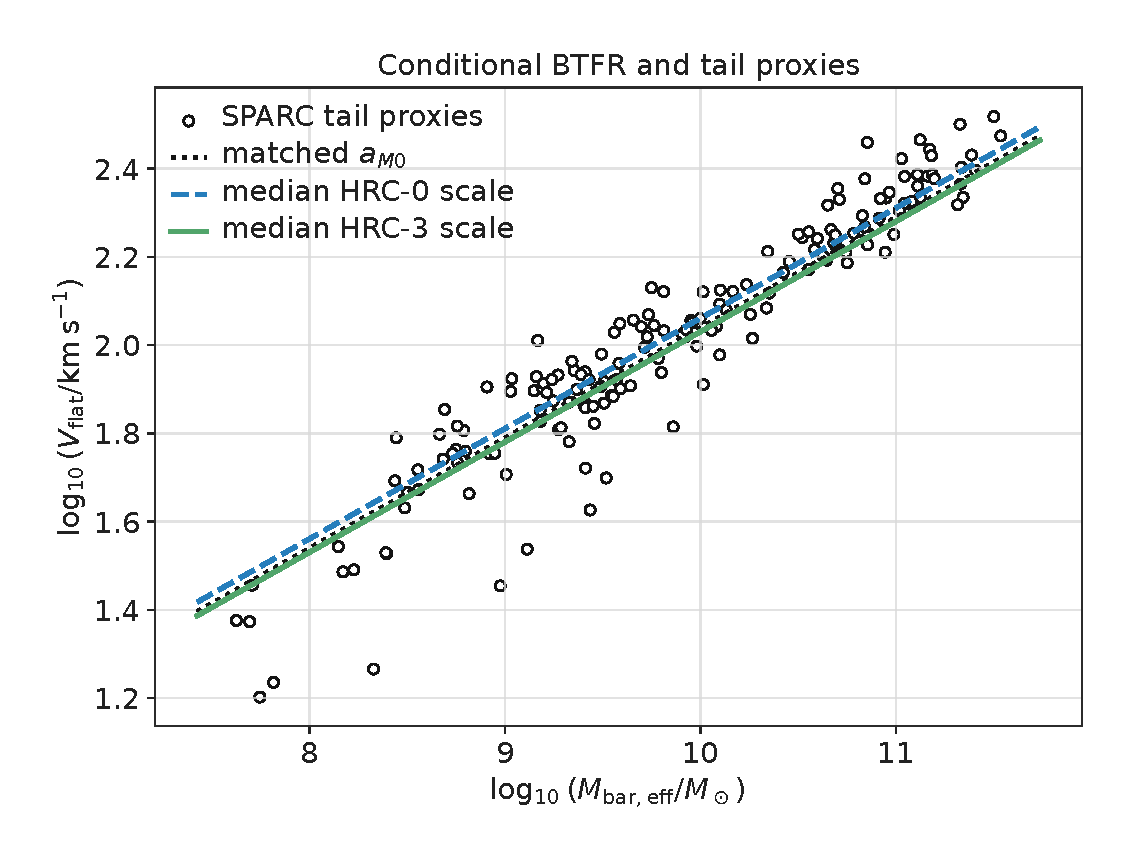
\includegraphics[width=\textwidth,height=0.76\textheight,keepaspectratio]{figures/r123/global/panels/fig15_a_btfr_tail_proxy_r123.pdf}
\caption{HRC-only BTFR diagnostic.  This page shows SPARC outer-tail
baryonic-mass proxies with the conditional slope-four relations evaluated at
the matched scale and the two fixed-$M/L$ median scales.  Because the mass
proxy comes from the same baryonic decomposition, this is an internal
pipeline check rather than an independent catalogue BTFR likelihood.  The
per-galaxy fitted-scale distributions follow as a separate full-width
continuation.  Colour is redundant with line style, marker shape, luminance
contrast and direct labels; no texture distinguishes the HRC models.}
\label{fig:btfr_new_main}
\end{figure*}

\begin{figure*}[!htbp]
\centering
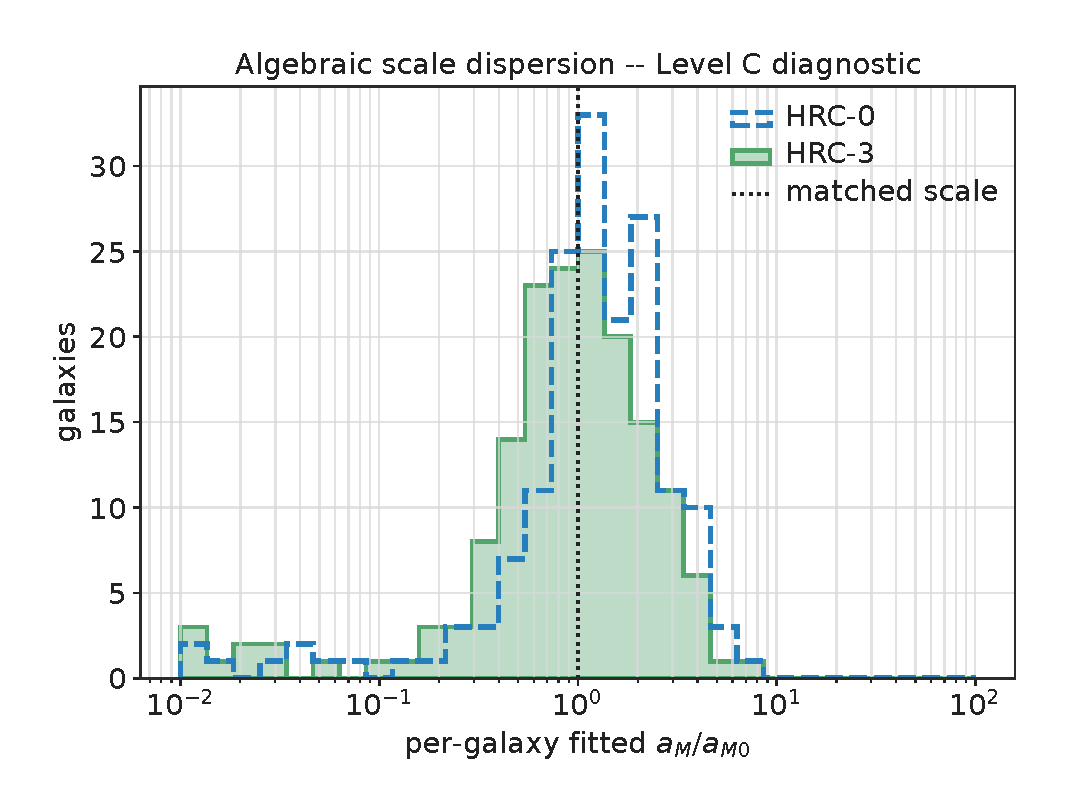
\includegraphics[width=\textwidth,height=0.76\textheight,keepaspectratio]{figures/r123/global/panels/fig15_b_scale_dispersion_r123.pdf}
\caption*{\textbf{Figure~\ref{fig:btfr_new_main}, continued.} Per-galaxy fitted-scale dispersion.  Its breadth also contains distance, inclination, stellar-population, bulge, non-circular-motion and algebraic-disk systematics.}
\end{figure*}

\paragraph{Orientation-sector separation.}
The live scalar-only reduction supplies no independent orientation triplet in
the galactic action.  A future covariant orientation term could modify the
response, but its source, sign and coefficient are not presently available.
No such term is included in the HRC diagnostics below.

\subsubsection*{HRC algebraic SPARC diagnostic}

For a symmetry-reduced field, the HRC relation used in the frozen diagnostic
is implicit:
\begin{equation}
 g_N(R)=\mu_{g,k}\!\left(\frac{g^2(R)}{a_M^2}\right)g(R),
 \qquad k\in\{0,3\},
 \label{eq:ect_rotation_closure_main}
\end{equation}
where $\mu_{g,0}$ and $\mu_{g,3}$ are obtained from
Eqs.~\eqref{eq:hrc0_mu_candidate} and~\eqref{eq:hrc3_weight_candidate}.
This numerical registry uses the explicit identity bridge
Eq.~\eqref{eq:hrc_identity_bridge}; a nontrivial $s=f(Y_g)$ would define a
different gravitational response even if the internal ERP response were
unchanged.
The baryonic input is
\begin{equation}
 g_N(R)=
 \frac{
 V_{\rm gas}|V_{\rm gas}|+
 \Upsilon_{\rm d}V_{\rm disk}^2+
 \Upsilon_{\rm b}V_{\rm bul}^2
 }{R}.
 \label{eq:gn_sparc_main}
\end{equation}
The signed gas term is essential.  The present calculation applies the local
relation~\eqref{eq:ect_rotation_closure_main} radius by radius.  For a generic
disk this is an approximation to the nonlinear three-dimensional equation:
\begin{equation}
 \mu\boldsymbol g
 =\boldsymbol g_N+\boldsymbol\nabla\times\boldsymbol H .
 \label{eq:hrc_disk_curl_guard}
\end{equation}
The available SPARC table contains mid-plane component velocities rather than
the full three-dimensional source, vertical scale-height priors and boundary
data.  It therefore cannot determine the curl field or supply a final disk
verdict.

\paragraph{Frozen protocol.}
The current Level-C diagnostic contains 165 SPARC galaxies, signed gas,
five whole-galaxy held-out folds repeated for five seeds, and two declared
stellar-$M/L$ modes.  The fixed-$M/L$ mode uses 3343 points per seed.  The
common-$M/L$ transfer mode fixes its validity mask at the lower bound
$\Upsilon_{\rm d}=0.3$ and therefore uses 3342 points per seed.  Only HRC-0 and HRC-3 are evaluated in the figures and table below.  The
results are:

\small
\begingroup
\setlength{\tabcolsep}{5.97pt}
\begin{longtable}{@{}L{0.15\linewidth}C{0.22\linewidth}C{0.10\linewidth}C{0.22\linewidth}C{0.205\linewidth}@{}}
\caption{HRC-only algebraic SPARC diagnostics.  These are absolute held-out
statistics of the local relation~\eqref{eq:ect_rotation_closure_main}, not a
full survey likelihood.}
\label{tab:sparc_summary_main}\\
\toprule
Response & Fixed-$M/L$ $\langle\chi^2\rangle$ & Fixed-$M/L$ SD &
Common-$M/L$ $\langle\chi^2\rangle$ & Fixed-$M/L$ fitted $\langle a_M\rangle$ / m\,s$^{-2}$ \\
\midrule
\endfirsthead
\toprule
Response & Fixed-$M/L$ $\langle\chi^2\rangle$ & Fixed-$M/L$ SD &
Common-$M/L$ $\langle\chi^2\rangle$ & Fixed-$M/L$ fitted $\langle a_M\rangle$ / m\,s$^{-2}$ \\
\midrule
\endhead
\bottomrule
\endfoot
HRC-0 & 117598.72 & 3645.86 & 109439.95 & $1.75\times10^{-10}$ \\
HRC-3 & 99501.19 & 2967.18 & 103763.46 & $1.27\times10^{-10}$ \\
\end{longtable}
\endgroup
\normalsize

The corresponding fold-averaged training values of $a_M$ in the
common-$M/L$ transfer mode are $1.2629\times10^{-10}\,{\rm m\,s^{-2}}$
for HRC-0 and $1.1170\times10^{-10}\,{\rm m\,s^{-2}}$ for HRC-3.  These
values are reported separately because they belong to a different
stellar-$M/L$ protocol from the final column of the table.
Across the five frozen whole-galaxy fold seeds, the population standard
deviations of the common-$M/L$ held-out $\chi^2$ totals are $3194.14$ for
HRC-0 and $4537.24$ for HRC-3.

The absolute scale $\chi^2/{\rm point}\sim30$ is a warning, not evidence of a
precision fit.  The current likelihood omits covariance, intrinsic scatter,
distance and inclination marginalisation, hierarchical stellar populations,
the external-field response and the full disk equation.  HRC-3 was formulated
after the crossover residual was inspected and is not an independent
prediction.

As a separate joint nuisance test, the baseline varies only
$10^{-2}\leq a_M/a_{M0}\leq10^2$ per galaxy at fixed
$\Upsilon_{\rm d}=0.5$ and $\Upsilon_{\rm b}=0.7$.  The comparison jointly
varies that same scale and an independent disk ratio
$0.1\leq\Upsilon_{\rm d}\leq2.5$ per galaxy while keeping
$\Upsilon_{\rm b}=0.7$.  It therefore probes the
$a_M$--disk-$M/L$ degeneracy rather than a free-$M/L$-only model.  The median
reduced $\chi^2$ changes from
$2.449$ to $1.293$ for HRC-0 and from $2.327$ to $1.273$ for HRC-3.  The
corresponding median scale ratios move from $1.222$ to $0.912$ and from
$0.921$ to $0.812$.  This improvement measures the expected
$a_M$--$M/L$ degeneracy, not additional support for a non-universal physical
scale.  A population prior and joint distance/inclination inference are still
required.  The fitted tails are boundary-censored: for HRC-0/HRC-3 the fixed
scale reaches its lower bound in 2/3 galaxies and the free-$M/L$ scale in 6/6;
$\Upsilon_{\rm d}$ reaches the lower bound in 21/19 and the upper bound in
14/9 galaxies.  These objects are retained as stress diagnostics, not used to
infer an uncensored physical scale distribution.

\begin{figure*}[!htbp]
\centering
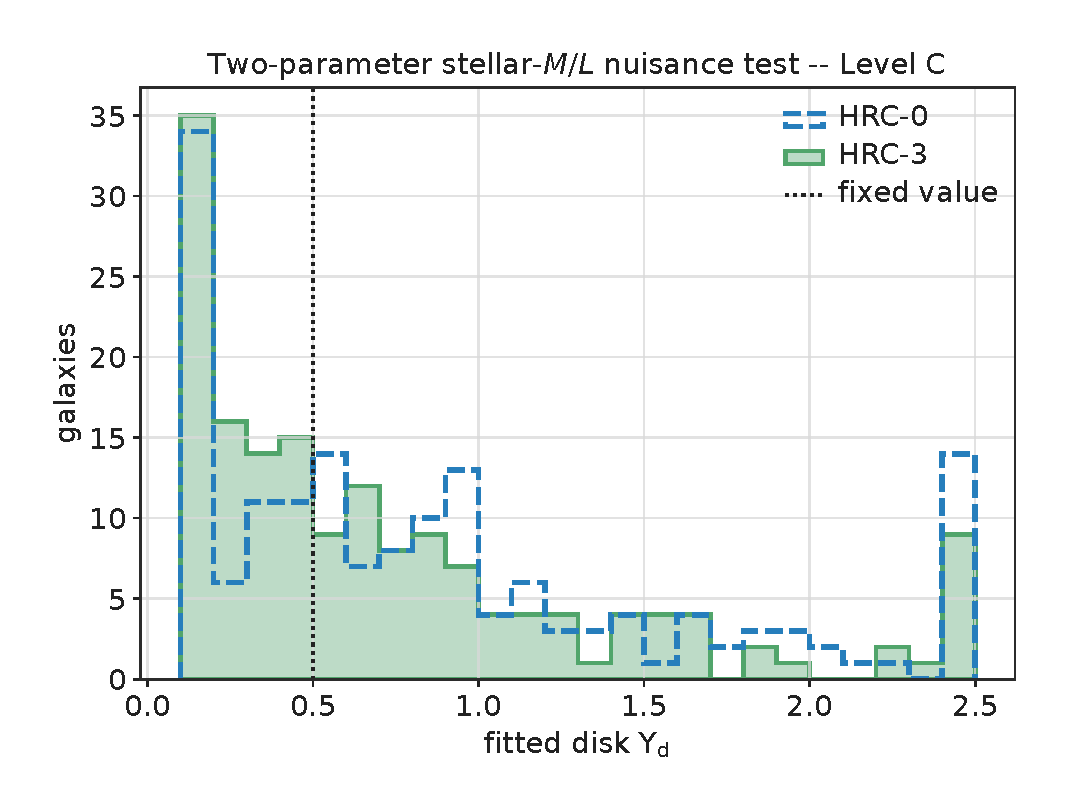
\includegraphics[width=\textwidth,height=0.68\textheight,keepaspectratio]{figures/r123/global/panels/fig16_c_two_parameter_nuisance_r123.pdf}
\caption{HRC-only stellar-$M/L$ sensitivity.  The first two panels compare
fixed- and free-$M/L$ fitted scales; the third gives the fitted disk
mass-to-light distributions.  The diagonal and fixed value are shown by
dotted black lines.  Boundary accumulation near $\Upsilon_{\rm d}=0.1$ or
$2.5$, and at the disclosed $a_M/a_{M0}=0.01$ lower bound, is a
nuisance-model warning; distribution tails are censored.  Complementary full-width panels are retained in Appendix~\ref{app:r129_visual_hrc_rotation}.}
\label{fig:hrc_scale_analysis_main}
\end{figure*}
\FloatBarrier

\paragraph{Reading the response-law panel.}
The preceding nuisance test concerns fitted stellar inputs and the declared
acceleration scale.  Figure~\ref{fig:chi2_comparison_main} now isolates the
response functions themselves, before the external rotation-curve examples
are introduced; no fit protocol or claim status changes at this transition.

\begin{figure*}[!htbp]
\centering
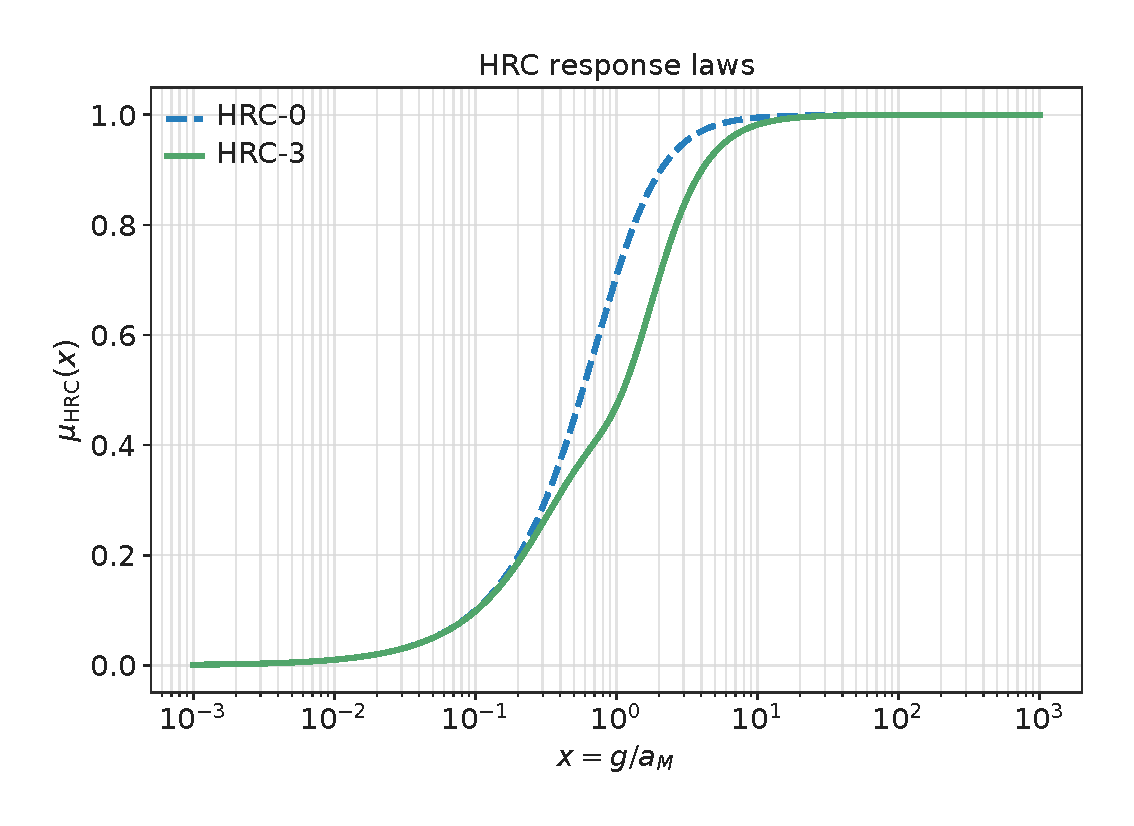
\includegraphics[width=\textwidth,height=0.68\textheight,keepaspectratio]{figures/r123/global/panels/fig17_a_response_laws_r123.pdf}
\caption{HRC-only response-law diagnostic.  This page compares the
exact HRC-0 response in the augmented inverse-DtN/recruitment model with the
conditional HRC-3 response.  The held-out deep/crossover/Newtonian
$\chi^2$-regime census is a separate full-width atlas panel.  Colour is
redundant with line style, marker shape, border contrast and direct labels,
so the figure remains legible in grayscale without decorative hatching.}
\label{fig:chi2_comparison_main}
\end{figure*}
\FloatBarrier

\paragraph{External model-comparison guard.}
Figures~\ref{fig:sparc_external_model_comparison_r123_a}--%
\ref{fig:sparc_external_model_comparison_r123_c} hold the baryonic
decomposition and stellar mass-to-light ratios fixed while separating a
fixed-input response comparison from a two-parameter Navarro--Frenk--
White (NFW) halo fit~\cite{NavarroFrenkWhite1997}.  HRC-0 is not
shape-distinct from the standard MOND interpolation used here: at equal
acceleration scale the two curves coincide identically.  Conversely, an NFW
fit is not a unique $\Lambda$CDM curve; it becomes a population-level
$\Lambda$CDM prediction only after halo-population, concentration--mass,
abundance, feedback and nuisance priors are supplied.  The six systems were
fixed before the rendering pass and do not establish survey-level model
selection.  Every panel uses $\Upsilon_{\rm d}=0.5$,
$\Upsilon_{\rm b}=0.7$, signed gas and a $2\,\mathrm{km\,s^{-1}}$ error
floor.  Colour is redundant with line style, markers and direct labels; no
hatch is used.  The comparison remains a local algebraic disk diagnostic,
not a finite-thickness field solution or hierarchical likelihood.  SPARC
measurements are shown only as unconnected error-bar markers.  Source model
ordinates are retained as faint, unconnected nodes.  Smooth traces are
residual-gated, shape-preserving display approximations through
curvature-regularised display nodes, with a maximum node-displacement
tolerance constrained to \(0.10\)--\(0.25\,\mathrm{km\,s^{-1}}\).  All fit
and diagnostic metrics use the original nodes; no continuous physical owner
is implied by a display trace.

\begin{figure*}[p]
\centering
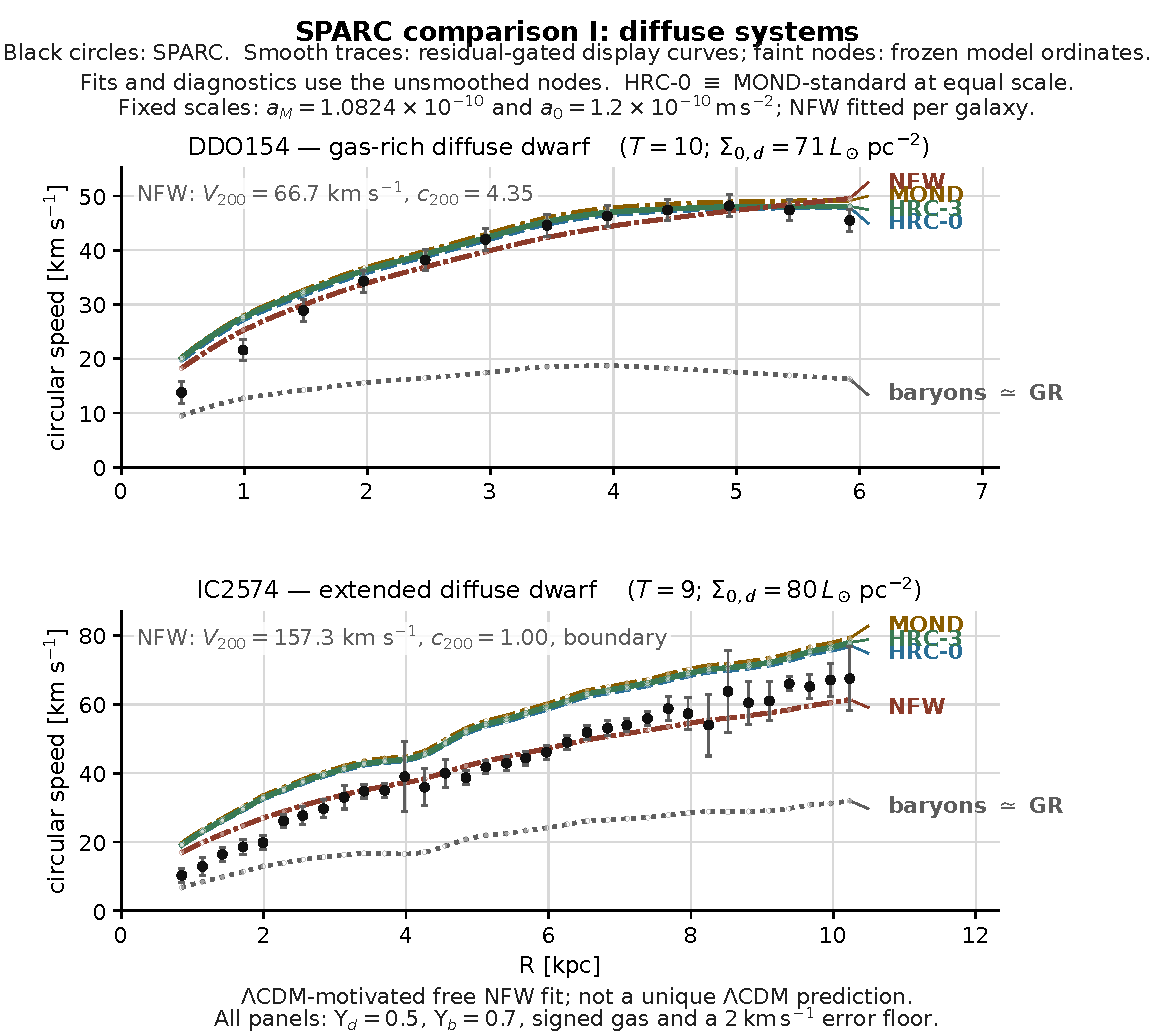
\includegraphics[width=\textwidth,height=0.70\textheight,keepaspectratio]{figures/r154/curve_semantics/main/R154_SPARC_SMOOTH_DISPLAY_A.pdf}
\caption{Representative SPARC external-model comparison, set~I.  DDO154 and
IC2574 sample diffuse and low-surface-brightness regimes.  Black
points are SPARC velocities; directly labelled curves show baryon-only
weak-field GR, fixed-scale MOND-standard, HRC-0, conditional HRC-3 and a
separately fitted two-parameter NFW halo.  HRC-0 and MOND-standard have the
same response shape and differ here only through their declared scales.  The
HRC matching input is $a_M=cH_0/(2\pi)$ at the externally declared
$H_0=70\,\mathrm{km\,s^{-1}\,Mpc^{-1}}$; its coefficient and ECT physical
owner remain Open.  LambdaCDM-motivated free NFW fit; fitted to the displayed rotation curve; not a unique LambdaCDM prediction.  Fixed baryonic inputs and boundary-hit flags are
printed in the figure.  This is a Level-C algebraic diagnostic, not a
population model-selection result.  The full comparison atlas in
Appendix~\ref{app:r129_visual_hrc_rotation} applies the same
externally guarded comparison to held-out, stratified-gallery and post-hoc
stress examples.}
\label{fig:sparc_external_model_comparison_r123_a}
\end{figure*}

\begin{figure*}[p]
\centering
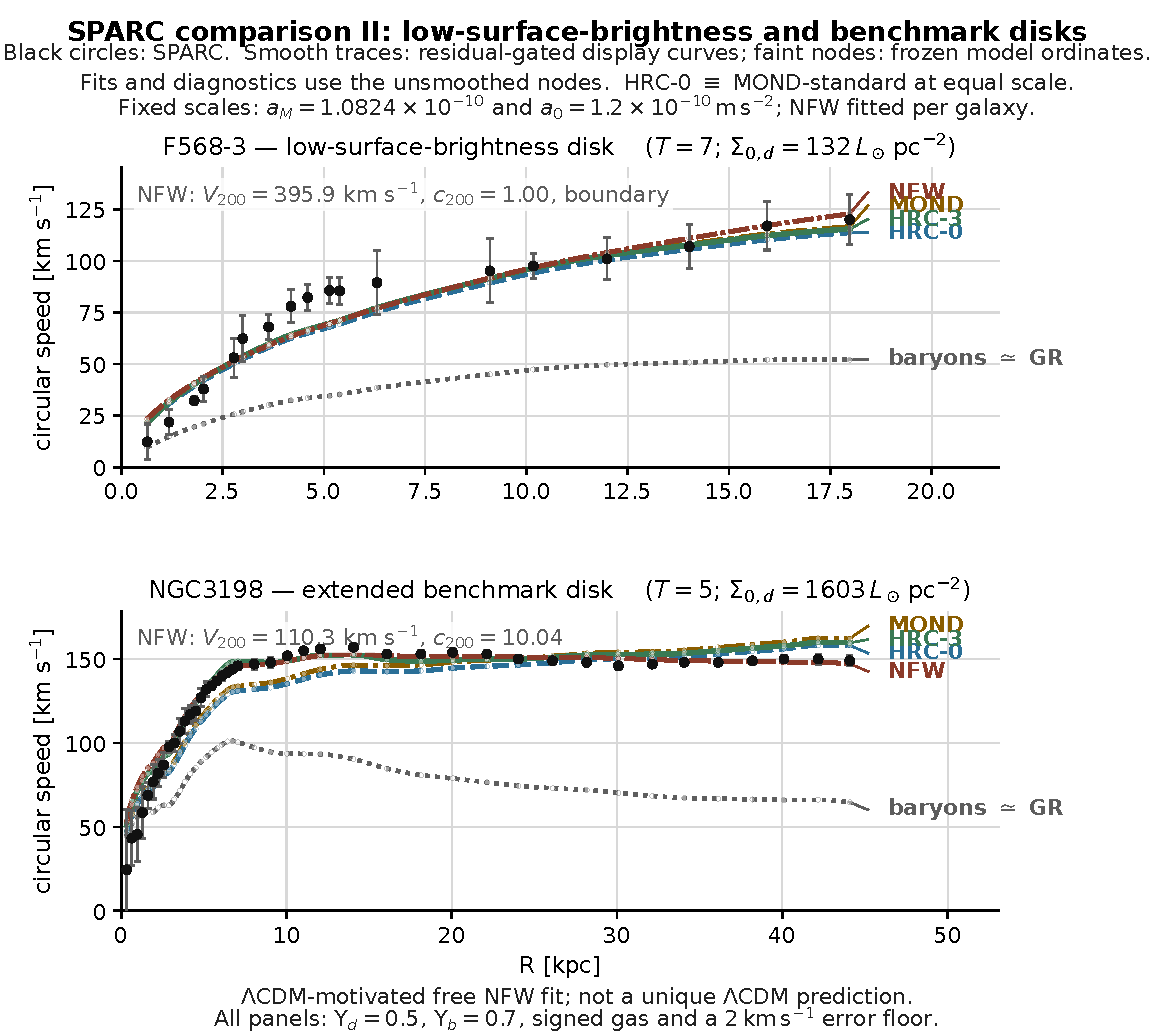
\includegraphics[width=\textwidth,height=0.70\textheight,keepaspectratio]{figures/r154/curve_semantics/main/R154_SPARC_SMOOTH_DISPLAY_B.pdf}
\caption{Representative SPARC external-model comparison, set~II.  F568-3
and NGC3198 provide low-surface-brightness and extended benchmark cases.
Black points and directly labelled curves use the
same fixed baryonic inputs as set~I: baryon-only weak-field GR,
MOND-standard, HRC-0, conditional HRC-3 and a separately fitted two-parameter
NFW halo.  The HRC matching input is $a_M=cH_0/(2\pi)$ at the externally
declared $H_0=70\,\mathrm{km\,s^{-1}\,Mpc^{-1}}$; its coefficient and ECT
physical owner remain Open.  Printed $V_{200}$ and $c_{200}$ are fitted separately.  LambdaCDM-motivated free NFW fit; fitted to the displayed rotation curve; not a unique LambdaCDM prediction.  The residual patterns expose where the fixed-scale
HRC/MOND curves or fitted halo are stressed.  This is a Level-C six-example
diagnostic, not survey-level model selection.}
\label{fig:sparc_external_model_comparison_r123_b}
\end{figure*}

\begin{figure*}[p]
\centering
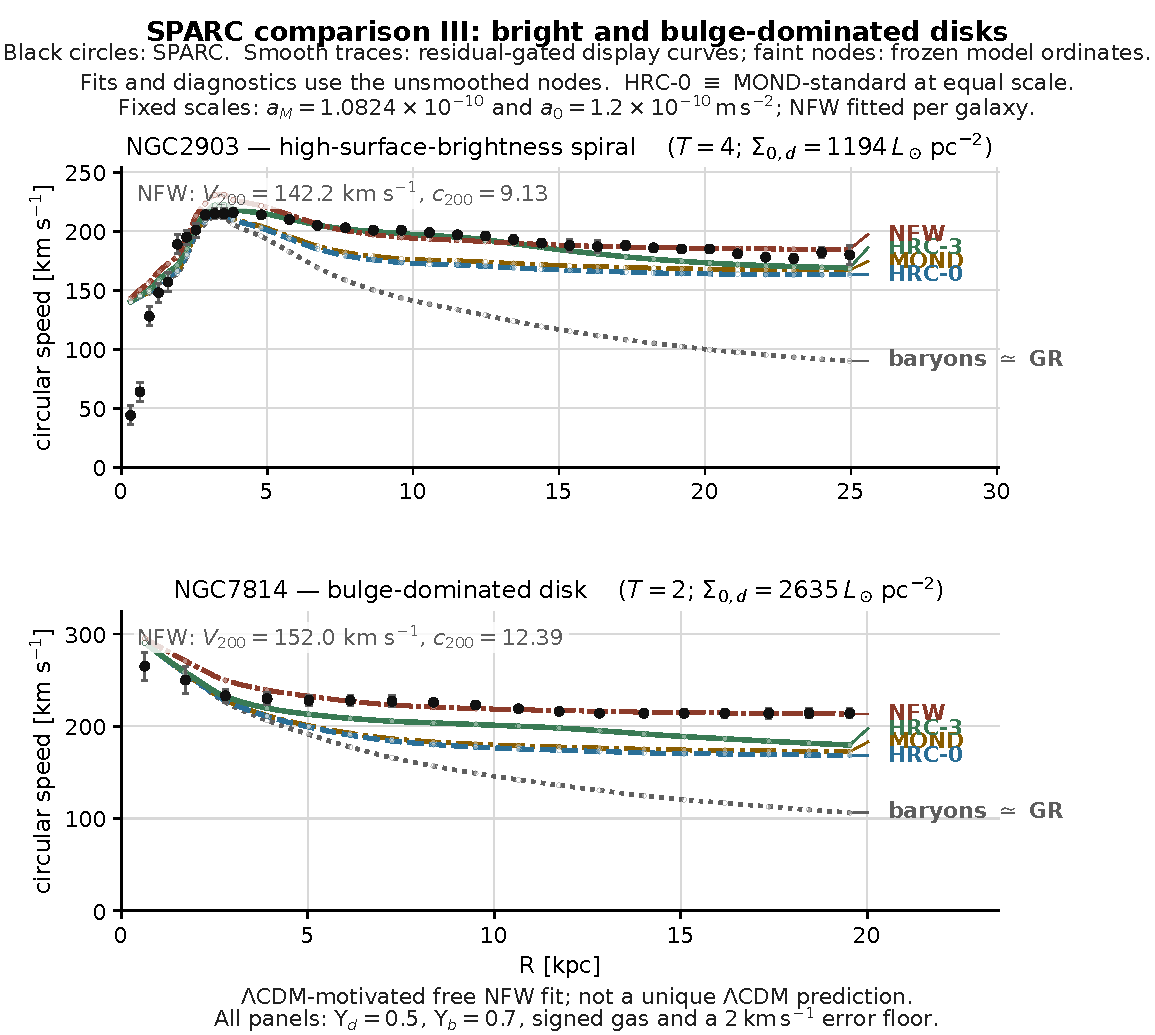
\includegraphics[width=\textwidth,height=0.70\textheight,keepaspectratio]{figures/r154/curve_semantics/main/R154_SPARC_SMOOTH_DISPLAY_C.pdf}
\caption{Representative SPARC external-model comparison, set~III.  NGC2903
and NGC7814 provide high-surface-brightness and bulge-dominated cases.
Black points and directly labelled curves use the same fixed baryonic inputs
as sets~I--II: baryon-only weak-field GR, MOND-standard, HRC-0, conditional
HRC-3 and a separately fitted two-parameter NFW halo.  The HRC matching input
is $a_M=cH_0/(2\pi)$ at the externally declared
$H_0=70\,\mathrm{km\,s^{-1}\,Mpc^{-1}}$; its coefficient and ECT physical
owner remain Open.  The printed $V_{200}$ and $c_{200}$ are fitted
separately.  The NFW curve is a $\Lambda$CDM-motivated free fit to the
displayed rotation curve, not a unique $\Lambda$CDM prediction.  This is a
Level-C six-example diagnostic, not survey-level model selection.}
\label{fig:sparc_external_model_comparison_r123_c}
\end{figure*}
\FloatBarrier

\par\noindent\textit{Reader guide.}  The three preceding pages form one
fixed-baryonic external-comparison suite, following the two locally placed
nuisance and response-law checks above.  They remain Level-C diagnostics,
not population-level model-selection results.  Appendix~\ref{app:r129_visual_hrc_rotation}
supplies a full-width comparison atlas with baryon-only weak-field GR,
MOND-standard, HRC-0, conditional HRC-3 and a separately fitted two-parameter
NFW benchmark for every displayed galaxy; the NFW curves are
$\Lambda$CDM-motivated fits, not unique $\Lambda$CDM predictions.




\paragraph{Scale status.}
The present matching value is
\begin{equation}
 a_{M0}=\frac{cH_0}{2\pi}
 \approx1.08\times10^{-10}\,{\rm m\,s^{-2}}
 \quad(H_0=70\,{\rm km\,s^{-1}\,Mpc^{-1}}),
 \label{eq:aM_baseline}
\end{equation}
but the coefficient is not derived.  A possible environment/history response
is only a test family,
\begin{equation}
 a_{M,{\rm eff}}=a_{M0}\,
 \Xi(\rho_{\rm env},\bar q_{\rm env},{\rm history},\ldots),
 \label{eq:aM_environment}
\end{equation}
with variables, sign and amplitude Open.  No Milky-Way-specific HRC result is
implied by this ansatz.

\subsubsection*{Milky Way sensitivity test}

The representative HRC sensitivity calculation uses 14
$4$--$25$~kpc velocity points representative of the Eilers et
al.\ reconstruction~\cite{Eilers2019} and a declared exponential disk
($M_{\rm d}=5.0\times10^{10}M_\odot$, $R_{\rm d}=2.5$~kpc).  It is a
sensitivity calculation, not a modern Milky-Way posterior: gas, bulge, halo
geometry, correlated systematics and baryonic-model uncertainty are absent.
The algebraic best fits are
\begin{equation}
 \begin{array}{c|cc}
 & a_M/a_{M0} & \chi^2_{\rm red} \\
 \hline
 \text{HRC-0} & 2.798 & 1.813 \\
 \text{HRC-3} & 1.703 & 2.287
 \end{array}
 \label{eq:hrc_milky_way_sensitivity}
\end{equation}
for this fixed disk.  The fitted displacement from $a_{M0}$ is therefore a
stress on the simplified baryonic model/universal-scale pair, not evidence
for a measured environment law.

\par\noindent The readable HRC-only Milky-Way sensitivity curve is retained as provenance in Appendix~\ref{app:r129_visual_hrc_rotation}; it is not a main-text external-model comparison.


\FloatBarrier
\subsection{Radial Acceleration Relation in the HRC diagnostic}
\label{sec:rar_subsection}

The observed and baryonic accelerations are
\begin{equation}
 g_{\rm obs}=\frac{V_{\rm obs}^2}{R},
 \qquad
 g_N=\frac{V_{\rm bar}^2}{R},
\end{equation}
and the symmetry-reduced conditional HRC response law is
\begin{equation}
 g_N=\mu_{g,k}(g_{\rm obs}^2/a_M^2)g_{\rm obs},
 \qquad k\in\{0,3\}.
 \label{eq:rar_ect_new}
\end{equation}

\begin{figure}[htb]
\centering
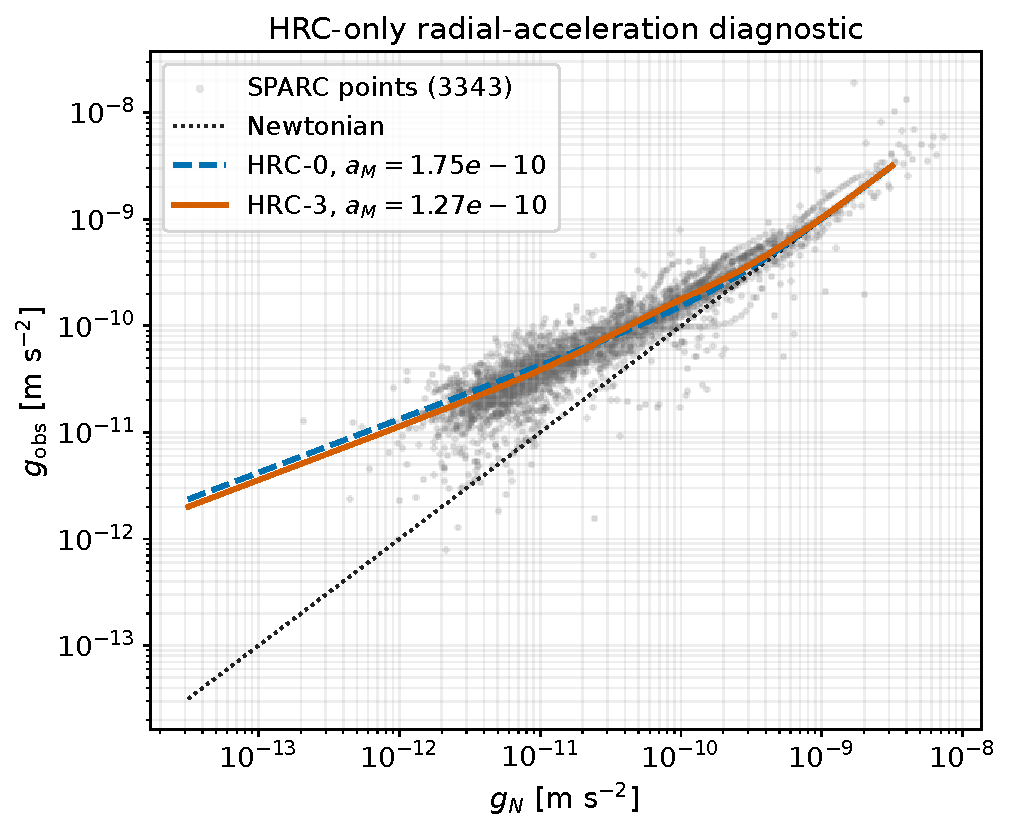
\includegraphics[width=\linewidth]{figures/r149/R97_HRC_RAR_DIAGNOSTIC_typography_r149.pdf}
\caption{HRC-only RAR diagnostic.  Grey points are the 3343 SPARC entries;
the HRC curves use the mean held-out fitted scales of the frozen algebraic
pipeline.  The plot is a Level-C diagnostic and does not include the disk curl
field, covariance or hierarchical nuisance model.  Colour is redundant with
line style.}
\label{fig:rar_new_main}
\end{figure}

As shown in Figure~\ref{fig:rar_new_main}, the deep and Newtonian
asymptotes are fixed by the declared HRC laws, whereas the crossover
distinguishes HRC-0 from HRC-3.  A claim of an ECT RAR prediction
requires both the missing medium-to-gravity bridge and a prespecified
full-field calculation.

\FloatBarrier
\subsection{Dark-matter-deficient ultra-diffuse galaxies as an HRC stress test}
\label{sec:udg_stress_test}

For a spherical central-value proxy, define
$\mathcal R_{\rm dyn}=g_{\rm obs}/g_N$.  The HRC equation admits a finite
positive-$a_M$ enhancement solution only when $\mathcal R_{\rm dyn}>1$;
equality is the Newtonian boundary $a_M=0$.  For HRC-0 the
required scale is obtained analytically:
\begin{equation}
 \frac{a_M^{(0)}}{g_{\rm obs}}
 =\sqrt{\mathcal R_{\rm dyn}^2-1}.
 \label{eq:main_udg_hrc0_inverse}
\end{equation}
For HRC-3, $x_3$ is the unique positive solution of
$\mu_{g,3}(x_3^2)=1/\mathcal R_{\rm dyn}$ and
$a_M^{(3)}=g_{\rm obs}/x_3$.

Using $R_{1/2}=4R_e/3$, enclosed stellar mass $M_\star/2$ and
$g_{\rm obs}=3\sigma^2/R_{1/2}$ gives the central proxy values below.
The pressure-supported inputs are drawn from the DF2/DF4, FCC~224,
NGC~5846-UDG1 and Dragonfly~44 literature
\cite{vanDokkum2018,Danieli2022DF4,Buzzo2025FCC224,Tang2025FCC224,
Trujillo2019DF2,Shen2021DF2TRGB,Forbes2021NGC5846UDG1,
vanDokkum2019DF44Kinematics}; heterogeneous
measurement procedures mean that the rows are not a common-confidence
sample.  AGC~114905 is a gas-rich rotator
\cite{ManceraPina2022AGC114905} and is excluded from the spherical proxy.

\small
\begin{longtable}{@{}L{2.9cm}L{2.0cm}L{2.2cm}L{2.2cm}L{4.2cm}@{}}
\caption{HRC-only central Wolf-proxy diagnostic.  Values are not a Jeans
posterior, and AGC~114905 requires a disk solver.}
\label{tab:udg_stress_test}\\
\toprule
Object & $\mathcal R_{\rm dyn}$ & $a_M^{(0)}/a_{M0}$ &
$a_M^{(3)}/a_{M0}$ & Domain/status \\
\midrule
\endfirsthead
\toprule
Object & $\mathcal R_{\rm dyn}$ & $a_M^{(0)}/a_{M0}$ &
$a_M^{(3)}/a_{M0}$ & Domain/status \\
\midrule
\endhead
\bottomrule
\endfoot
NGC~1052--DF4 & 0.787 & --- & --- & No positive HRC enhancement solution at central inputs \\
FCC~224 & 1.229 & 0.0155 & 0.00780 & Strong suppression of the matched scale required \\
NGC~1052--DF2 & 2.328--6.988 & 0.0476--0.470 & 0.0278--0.457 & Dispersion bracket remains ambiguous \\
NGC~5846-UDG1 & 10.262 & 0.947 & 0.935 & Close to the matched HRC scale \\
Dragonfly~44 & 31.734 & 4.951 & 4.944 & Scale substantially above the matched value \\
\end{longtable}
\normalsize

\begin{figure}[htb]
\centering
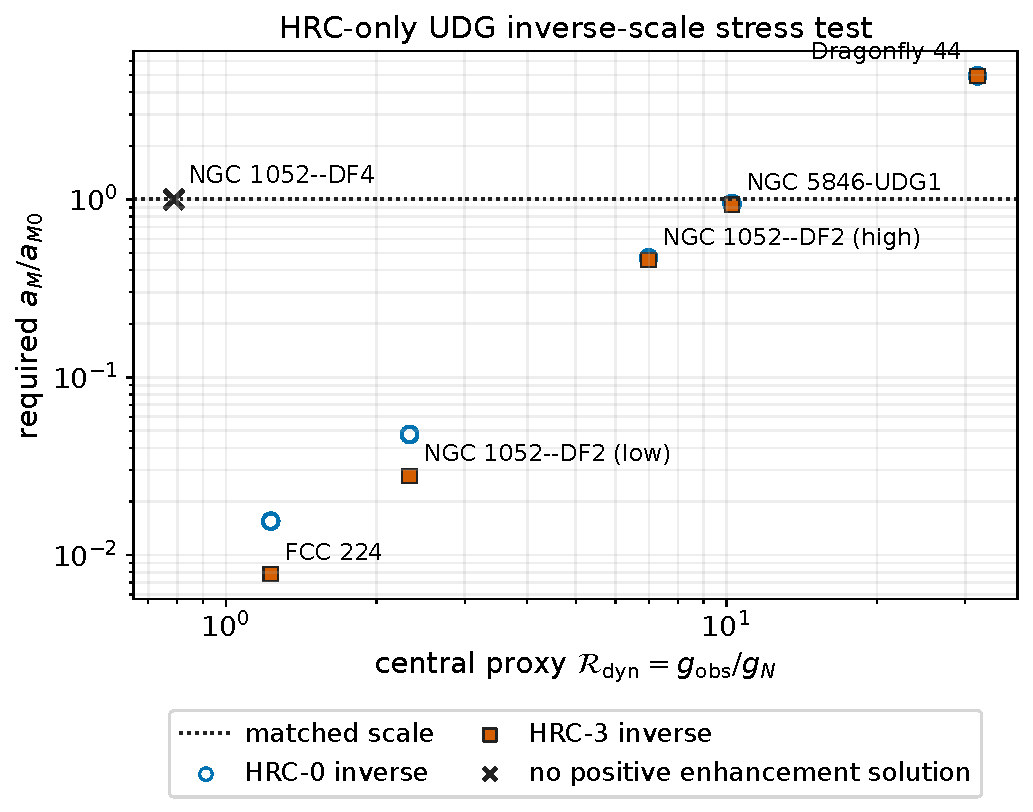
\includegraphics[width=\linewidth]{figures/r149/R97_HRC_UDG_STRESS_typography_r149.pdf}
\caption{HRC-only inverse-scale UDG stress test.  The two DF2 points are the
low- and high-dispersion endpoints; the cross marks a central proxy outside
the positive-enhancement domain.  The matched-scale line is not an
environment fit.  HRC-0 and HRC-3 nearly coincide for the largest
$\mathcal R_{\rm dyn}$, while they differ appreciably near the crossover.}
\label{fig:udg_regime_diagram}
\label{fig:udg_stress_test}
\end{figure}

Figure~\ref{fig:udg_regime_diagram} visualises the same central-proxy
stress test: similar diffuse systems require radically different effective
response scales, while DF4 is
outside the positive-enhancement domain at its central proxy inputs.  It does
not derive an environment law, explain the incidence rate, or supersede a
non-spherical Jeans analysis.  A successful completion must predict the
additional variable or history dependence rather than fitting a separate
$a_M$ to each object.

\paragraph{Finite completion tests.}
The galactic numerical sector is not complete until it supplies: (i) a
density-aware axisymmetric HRC solver; (ii) the external-field response in the
same operator; (iii) distance, inclination, covariance, intrinsic-scatter and
hierarchical-$M/L$ marginalisation; (iv) a prespecified independent galaxy
test; and (v) the covariant metric needed before any lensing, cluster, PPN or
cosmological use.

\subsection{Summary and status of galactic and cluster-scale phenomenology}
\label{sec:mp_galactic_summary}
% ==============================================================

This chapter records an HRC galactic diagnostic and a separate exact local-map
cluster theorem.  Its current result ledger is:
\begin{enumerate}
  \item The amplitude coordinate $\phi_u$ and the conditional homogeneous
    scalar response are available inside the Level-B scalar ansatz.  No
    AU--kpc--Mpc screening hierarchy is derived; canonical mass,
    body charge, and PPN reachability remain Open.
  \item The strictly increasing-map order/argmax theorem is Level~A
    inside the supplied local map: it preserves the complete ordering, the
    possibly empty set-valued argmax and every attained maximum of the supplied
    total projected baryon field.  No synthetic replay
    or amplitude result is retained.  The physical cluster map, collision
    dynamics and general causal merger kernel remain Open.
  \item The 165-galaxy SPARC statistics and associated figures have been
    recomputed with HRC-0 and HRC-3.  They are Level-C algebraic
    diagnostics and not a full field-level likelihood.
  \item HRC-0 and HRC-3 share the deep response $\mu\sim g/a_M$, so the
    BTFR slope~4 follows conditionally from the separate static gravity bridge.
    The normalisation $a_{M0}=cH_0/(2\pi)$ remains a matching condition.
  \item HRC-0 is exact in the augmented inverse-DtN/recruitment model and
    HRC-3 is conditional on the supplied three-channel matrix owner.  Their
    same-pipeline comparison is Level~C; full finite-disk fields and the
    publication cascade remain uncomputed.  The force-dimensionality curve
    uses the algebraically identical HRC-0 shape but is not retroactively
    promoted to a microscopic ECT derivation.  Residual scatter has no derived
    environment/history component, sign, or amplitude.
\end{enumerate}

\noindent
The HRC-only fit arithmetic is a Level~C algebraic diagnostic.
ERP-$\Phi$ is a new constitutive proposal; the HRC responses have
their model-conditional statuses stated in Sec.~\ref{sec:hrc_erp_candidate}.
The gravity bridge, environment law~$\Xi$, action/source matching and scalar
screening remain Open.  A known stress test of the HRC algebraic diagnostic is the class of
dark-matter-deficient ultra-diffuse galaxies (NGC~1052--DF4,
FCC~224); these are listed as entry ND-13 in
Table~\ref{tab:future_discriminants} and discussed diagnostically
in Appendix~\ref{app:udg_stress_test}, and the HRC-only central-proxy inversions are reported as stress
diagnostics, not as field-level explanations.
For the cosmological sector of the ordered-branch programme, see the
summary in Section~\ref{sec:mp_cosmo_status}.

% ==============================================================
\FloatBarrier
\section{Mass-discrepancy and late-time-acceleration phenomenology in ECT}
\label{sec:mp_dark}
% ==============================================================

\textit{Status: mixed.  The scalar--tensor ansatz and late-time
background closure are Level B at their declared scope.  The galactic HRC-only algebraic outputs are Level-C diagnostics.  ERP-$\Phi$/HRC is the active
candidate programme: exact or conditional in its stated augmented response
models, but its P1--P6 and gravity ownership remains Open.  Additional
condensate dark sectors and the cosmological fraction budget remain Open.}

This section separates galactic mass-discrepancy fits, possible additional
collective excitations, and late-time background acceleration.  The absence
of a particle halo is a property of the conditional HRC algebraic diagnostic, not an
ECT theorem about particle content.

\subsection{Scope and dark-sector logic}
\label{sec:dark_sector}

The present manuscript separates three model questions without claiming a
derived common ontology.  First, the separately supplied conditional HRC gravity
functional G contains no particle-halo term and is evaluated against selected benchmarks;
its scalar/ECT matching and fundamental particle content are Open.  Second,
the late-time scalar-background ansatz parametrises accelerated expansion;
its microscopic origin, uniqueness, and cosmological matter budget are Open.
Third, possible particle, collective, defect, or topological sectors are
research candidates with no derived abundance or assigned cosmological role.

P4, P6, and the branch architecture do not by themselves identify the
galactic fit with $\phi_u$, derive a dark-energy source, or exclude hidden
components.  The separation below is therefore an organisational status
ledger, not a postulate-grounded derivation of the dark sector.

\begin{longtable}{@{}L{2.80cm}L{4.40cm}L{3.30cm}L{4.10cm}@{}}
\caption{Three distinct dark-sector questions in the present ECT programme.}
\label{tab:dark_sector_channels}\\
\toprule
Question & Present statement & Status & Next discriminating gate \\
\midrule
\endfirsthead
\multicolumn{4}{l}{\textit{Table~\ref{tab:dark_sector_channels} continued}}\\
\toprule
Question & Present statement & Status & Next discriminating gate \\
\midrule
\endhead
\midrule
\multicolumn{4}{r}{\textit{Continued on next page}}\\
\endfoot
\bottomrule
\endlastfoot
Galactic mass-discrepancy response
& HRC-0/HRC-3 are active augmented-model candidates with current
algebraic no-halo diagnostics; the full field solve remains Open
& A/B/C by layer; live ECT Open
& HRC disk likelihood; derive the medium, source and metric map \\
Late-time acceleration
& The two-slope action supplies a regular proof of class; a trace-free
  completion supplies independent shift covariance through $C_I$
& A in supplied actions / C benchmark / ECT Open
& Derive the $\Phi$-medium action and state, physical metric, perturbations,
  and joint likelihood \\
Additional sectors
& Particle, collective, defect, and topological candidates have no derived
abundance or assigned dark-sector role
& Open
& Spectrum, stability, production, abundance, coupling, lensing, and growth \\
\end{longtable}

\subsection{HRC no-halo algebraic diagnostic and Open particle content}
\label{sec:dark_matter_interp}
% ==============================================================

\subsubsection*{HRC no-halo diagnostic and Open particle content}

The conditional HRC static functional contains no particle-halo term and is
evaluated on selected flat-curve, RAR, and BTFR benchmarks.  Its absolute
held-out likelihood is poor; this is a property of the specified diagnostic, not a derivation that ECT selects the functional and
not evidence that particle dark matter is absent.  The amplitude coordinate
is motivated by the Level-B scalar ansatz, whereas the AQUAL-type functional,
its source/force map, the origin of $a_M$, and the environment law $\Xi$
have not been derived from that ansatz.

\paragraph{Status and discriminator.}
The current result is therefore a Level-C no-halo fit benchmark with Open ECT
matching and Open fundamental particle content.  A particle species shown independently to explain the galactic
discrepancy would disfavor this minimal no-halo fit as a complete description,
not the ECT framework.  Conversely,
null direct-detection searches do not confirm the closure.

\paragraph{Numerical anchors from Section~\ref{sec:mp_galactic_phenom}.}
Inside the declared functional, the BTFR slope~4 follows by exact conditional
algebra.  The baseline
$a_{M0}=cH_0/(2\pi)\approx1.08\times10^{-10}$\,m\,s$^{-2}$ is a
matched benchmark, the observed RAR scatter is
$\sigma\approx0.13$\,dex~\cite{McGaugh2016,Lelli2017}, and the SPARC
pipeline fits one $a_{M,\rm eff}$ per galaxy for 165 galaxies.  These
fit facts do not supply the missing scalar-to-galactic derivation or a
cosmological particle-fraction prediction.

\subsubsection*{Collective excitations and topological sectors}
\label{sec:ds_topological}

\textit{Status: Level~B/C structural possibilities. Relic abundance,
stability, and production history not yet computed from bare~P3.}

The ordered branch supports a constrained soft orientation sector.  Its
strict scalar map has one longitudinal coordinate $\chi$ at linear order;
one physical mode is a Level-B reduced-EFT interpretation.  Its dark-sector
role, abundance, and stability are not
established.  The HRC algebraic diagnostic does not use this mode or a
particle-halo term, but that fit property neither requires nor excludes
particle or collective dark sectors.

The topological completeness of the $\Phi$-medium~(S10) together with
the coherent branch~(BR1) admits the possibility that part
of the dark sector is tied to the smooth coherent-branch
configurations: winding sectors,
vortex-like structures, or topological configurations
(see Section~\ref{sec:predicted_states} for the full classification).
Their definition and dynamics depend on winding numbers and defect
stability beyond the coherent approximation.
They are noted here as a conceptual bridge to the Quantum
Sector~(Section~\ref{sec:qs_dark_sector}); their detailed
treatment is deferred.

\paragraph{No physical large-scale mass prediction.}
For any supplied relativistic mass parameter one may define a Compton scale
$\xi_G=\hbar/(m_Gc)$, but ECT derives neither a physical soft-mode mass
operator nor a value of~$m_G$.  The separately named
$m_{\chi,E}=\zeta_HH_{0,E}$ point is retained only as a nonpredictive C/Open
orientation benchmark, with its quoted reduced-Compton proxy.  It supplies
no physical or predicted Hubble-scale mass, coincidence explanation,
relic-abundance estimate or dark-sector inference.

The homotopy group $\pi_3(S^3)=\mathbb{Z}$ is structurally fixed for the
supplied orientation target.  Its identification with the complete physical
configuration space, and whether corresponding admissible configurations
are dynamically stabilised as particle-like or long-lived dark-sector
objects, remain Open.

Ultra-light modes and topological condensate configurations remain
candidate additional excitations.  They are not terms in the conditional HRC
algebraic diagnostic, but that omission neither excludes nor constrains their possible
abundance.  Any cluster or cosmological role remains Open.

\subsubsection*{Direct-detection discriminator and cosmological-fraction status}

The Level-C HRC algebraic diagnostic contains no particle-halo term and is
evaluated on selected rotation-curve benchmarks with poor absolute held-out likelihood.  This neither derives that ECT
selects the closure nor excludes particle dark matter, and it predicts no
absence of a laboratory particle signal.  A robust particle detection shown independently to explain the
galactic discrepancy would disfavor the minimal no-halo fit as a complete
description, not ECT as a whole.  Conversely, a
null direct-detection result does not confirm this closure.

ECT does not yet derive $\Omega_b$, $\Omega_{\rm DM}$, or $\Omega_\Lambda$
from first principles.  The galactic no-halo fit, the late-time background
closure, and possible condensate or particle excitations must therefore keep
separate status labels.  Their abundances, stability, mutual matching, and
cosmological roles remain Open.

% ==============================================================

\subsection{Late-time scalar stress: conditional lemma and open acceleration owner}
\label{sec:dark_energy_phi}

The amplitude coordinate in this subsection is
$\phi=\phi_u=\beta_\phi^{-1}\ln(u/u_\infty)$ on an ordered patch
$u>0$, not the distinct anisotropy coordinate
$\psi_K=\ln(\Delta_K/\Delta_{K,{\rm vac}})$.  The map between those
coordinates is Open.  Inside a supplied scalar completion,
Eqs.~\eqref{eq:rho_phi}--\eqref{eq:w_phi} give the exact bare-ratio lemma
\begin{equation}
 \omega>0,\quad K_\phi^{\rm phys}+U>0
 \quad\Longrightarrow\quad
 w_\phi^{\rm bare}=
 {K_\phi^{\rm phys}-U\over K_\phi^{\rm phys}+U}\ge-1.
 \label{eq:w_ect}
\end{equation}
The lemma is dimensionally correct Level~A algebra for the bare scalar pieces.
It neither derives the potential/state nor bounds the action-owned effective
history, because Eq.~\eqref{eq:rho_phi_nonminimal_bookkeeping} also contains
$\dot F$ and $\ddot F$.

\paragraph{Proof-of-class, not an ECT acceleration result.}
A selected $U(\phi)>0$ and a state with
$K_\phi^{\rm phys}\ll U$ give a vacuum-like bare scalar ratio, but
acceleration follows only from the full condition below.  In a non-minimally coupled completion the actual
acceleration also contains derivatives of $F(\phi)$ and must be obtained from
the complete metric equations.  Thus the existence of an admissible scalar
parametrisation is Level~B proof-of-class; ECT ownership is Open.  The action
does not identify a physical $w(a)$, a coincidence history, or any
redshift-dependent late-time-source likelihood.

\paragraph{Exact acceleration condition in the supplied scalar model.}
Combining the two Jordan-frame background equations gives
\begin{equation}
 {\ddot a\over a}
 =-{1\over6F}\left[
 {\rho_m+2\rho_r\over\bar M_{\rm Pl}^2}
 +2\omega\dot\phi^2-{2U\over\bar M_{\rm Pl}^2}
 +3(\ddot F+H\dot F)\right].
 \label{eq:ect_scalar_acceleration_condition}
\end{equation}
Therefore \(w_\phi^{\rm bare}\simeq-1\) is neither necessary nor sufficient by itself
when \(F\) evolves.  A supplied trajectory accelerates precisely when the
bracket in Eq.~\eqref{eq:ect_scalar_acceleration_condition} is negative.
This equality is an internal Level~A test of the supplied action and state;
the identification of that action with ECT remains Level~B/Open.

\paragraph{Two-slope late-time proof-of-class.}
The potential
\begin{equation}
 V_s(\sigma)=V_-e^{c_s\sigma}+V_+e^{b_s\sigma},
 \qquad F_s=F_*e^{a_s\sigma},\qquad K_s=\kappa_sF_s,
 \label{eq:ect_dark_energy_two_slope}
\end{equation}
has a finite stationary point of \(V_s/F_s^2\) when
\((c_s-2a_s)V_-+(b_s-2a_s)V_+=0\).  With
\(c_s<2a_s<b_s\) and positive coefficients, the effective potential is
bounded on both sides and the stationary point is a minimum.  This removes
the zero-density degeneration of a single exponential and supplies a
globally regular scalar-background example.  The nine calibrated numerical nodes in
Table~\ref{tab:two_slope_calibrated_scan_expanded} then show how the sampled
potential parameters affect age, distances, \(r_s\), Planck-scale drift and local
gravity; they do not establish a continuous-family trend.  It does not make the potential or its coefficients consequences of
P1--P6.

\paragraph{Effective equation of state as a derived diagnostic.}
For any solved trajectory define
\begin{equation}
 w_{\rm eff}(N)=-1-{2\over3}{H'(N)\over H(N)},\qquad
 q_{\rm dec}(N)=-1-{H'(N)\over H(N)}.
 \label{eq:ect_dark_energy_effective_diagnostics}
\end{equation}
These quantities describe the total expansion history and are the correct
background diagnostics even when the scalar stress cannot be separately
conserved.  They must be reported together with the decomposition into
matter, radiation, scalar kinetic/potential and \(F\)-derivative terms.
Fitting \(w_0,w_a\) is a compression of a solved trajectory, not a substitute
for solving it.

\paragraph{Coincidence and stability requirements.}
A physical late-acceleration mechanism must explain why the accelerating
regime occurs near the present state without selecting that state by a
terminal shooting condition.  Along the complete orbit the reduced scalar
mass, kinetic eigenvalues and characteristic speeds must remain physical,
and the same asymptotic state must pass finite-body PPN and varying-\(G\)
constraints.  A potential that accelerates only on a locally excluded branch
does not close the late-time sector.  This is a dynamical selection question,
not a prejudice against a constant contribution by itself; the distinction is
usefully emphasised in Ref.~\cite{BianchiRovelli2010}.

\paragraph{Current DESI context and conditional falsifier.}
DESI DR2 BAO are well described by flat $\Lambda$CDM in isolation.  When
combined with CMB and, dataset-dependently, supernova compilations,
$w_0$--$w_a$ fits prefer evolving dark energy; the quoted significance
varies with the data combination~\cite{DESIDR2_2025}.  The extended DESI
analysis finds a common low-redshift trend and a preference for phantom
crossing, while non-crossing alternatives are disfavoured but not excluded
~\cite{Lodha2025}.  This is observational context, not an ECT prediction or
a discovery claim.  For the positive-kinetic two-slope Jordan scalar the
bare bookkeeping ratio
$w_q=(K\dot\sigma^2/2-V)/(K\dot\sigma^2/2+V)$ obeys $w_q\ge-1$ when
$K\ge0$ and $\rho_q>0$; nonminimal $F$ terms mean that this bare ratio is
not the fitted action-owned effective $w(z)$.  A robust ECT completion whose
observable effective history is constrained never to cross $-1$ would be
disfavoured, but the present completion has not been run through the full
DESI+CMB+SN likelihood and is therefore untested.

\paragraph{Required observational comparison.}
The background test set is
\begin{equation}
 \{H(z),D_M(z),D_L(z),r_{\rm drag},t(z)\},
 \label{eq:ect_dark_energy_background_targets}
\end{equation}
while the perturbative test set is
\begin{equation}
 \{f\sigma_8,C_\ell^{\kappa\kappa},C_\ell^{Tg},
 C_L^{\phi\phi},D_L^{\rm GW}/D_L^\gamma\}.
 \label{eq:ect_dark_energy_perturbation_targets}
\end{equation}
One joint likelihood is required because a non-minimal \(F(\phi)\) changes
background distances, growth, photon lensing and local calibration
simultaneously.  Agreement in the first set with failure in the second rejects
the supplied completion.

\paragraph{Relation to the vacuum-offset result.}
The fixed determinant is an exact orientation-sector identity, not a
decoupling theorem.  Vacuum-offset shift covariance follows only in the
separately supplied trace-free completion, where $V+C_I$ is invariant under
opposite shifts.  The ordinary two-slope action can generate a positive,
stable late source but is not additive-shift invariant.  Neither statement
alone selects the source, magnitude or evolution observed in our condensate;
the action descent and observable matching remain Open.

\paragraph{Completion and falsification gates.}
A late-time ECT result requires one varied ordered-medium action to determine
$F$, $\omega$, $U$, the orientation stress and the state; one globally
regular stable background; a physical matter/photon metric; and a joint
background-plus-perturbation likelihood.  Only then can $w(a)$ and the sign
and magnitude of accelerated expansion be compared with observations.  A
failure rejects that named completion.  The full owner chain is given in
\S\ref{sec:ect_cosmology_closure} and
Appendix~\ref{app:ect_cosmology_observable_protocols}.

\subsection{Dark-sector discriminants and falsifiers of the present closure}
\label{sec:dark_discriminants}
% ==============================================================

This subsection separates closure-specific tests, imported
benchmarks, and Open research programmes relevant to dark-sector
interpretation.  The status-tagged inventory in
Table~\ref{tab:ECT_predictions} must not be read as a list of uniformly
derived ECT predictions.

\paragraph{Exploratory environment/history test (F1).}
The fitted scale $a_{M,\rm eff}$ may be cross-correlated with declared
environment and history covariates as a test of the Open law~$\Xi$.  The
corrected scalar equation does not derive the earlier
$\gamma\,4\pi\bar\rho_{\rm m}/U_0''$ combination, nor does it predict a
positive sign or a ten-percent amplitude.  A null result constrains the
specified regression model; a detected correlation does not by itself
establish the scalar source/screening chain or ECT.

\paragraph{Minimal-fit particle-halo scope test.}
The Level-C HRC algebraic diagnostic is fitted to the selected rotation-curve
sample and returns model outputs without a particle-halo term; its absolute
held-out likelihood is poor.  This is not a derivation that the
mass discrepancy in ECT must arise from that closure and is not a prediction
that particle dark matter is absent.
The LZ 4.2-tonne-year analysis reports a minimum observed 90\% C.L.
spin-independent WIMP--nucleon limit
$\sigma_{\rm SI}<2.2\times10^{-48}\,$cm$^2$ at a WIMP mass of
$40\,$GeV/$c^2$, with no positive WIMP signal~\cite{LZ2025}.
This external exclusion curve does not by itself determine whether any
particle species accounts for the galactic mass discrepancy.
A robust detection of a particle species specifically shown to account
for the galactic mass discrepancy would disfavor the minimal no-halo fit as a
complete description of that channel; it would not by itself falsify ECT.
Detection of a subdominant species would not decide the status of the Level-C HRC data diagnostic or its still-Open
ECT matching.

\paragraph{Bare scalar-ratio guard and physical falsifier.}
Equation~\eqref{eq:w_ect} tests only the bare scalar decomposition.  Because
the non-minimal terms in Eq.~\eqref{eq:rho_phi_nonminimal_bookkeeping} enter
the solved expansion history, an observational preference for
$w_{\rm eff}<-1$ does not contradict that identity.  It would reject a named
completion only if the complete action-owned background, photon/perturbation
map and likelihood independently constrained its observable
$w_{\rm eff}(a)$ never to cross $-1$.  Agreement with either sign would not
establish ECT ownership.

\paragraph{Local cluster-response no-go (F10).}
For any positive baryonic projected field and any strictly increasing local
map $F$, the response $\Sigma_{\rm resp}(\mathbf x)=F(\Sigma_b(\mathbf x))$
preserves the complete pointwise ordering and the set-valued identity
$\operatorname*{argmax}\Sigma_{\rm resp}=
 \operatorname*{argmax}\Sigma_b$, with both sets possibly empty.  Whenever
the maxima are attained, it therefore cannot dynamically displace a
total-response maximizer away from the supplied total-baryon maximizers or
encode merger memory.  This does not constrain the residual
$\Sigma_{\rm resp}-\Sigma_b$, which is generally non-monotone, or a gas/BCG
offset already supplied in $\Sigma_b$.  Bullet-like systems are empirical
targets for the Open retarded two-potential collision problem, not outputs of
the local algebraic HRC response.

\paragraph{Disambiguation of M, S, and G.}
The microscopic preferred-direction operator M, the Level-B scalar ansatz S,
and the conditional HRC static functional G are three distinct objects.
M is not S by operator and variable content; G is a phenomenological kpc
fit, while the map S$\to$G remains Open.  None may be used as a derived
surrogate for another in dark-sector comparisons.

\medskip\noindent
Taken together, these items have different statuses.  The bare scalar-ratio
identity is conditional algebra inside its scalar closure and does not bound the
physical background history; the cluster script is only an exact
peak-preservation sanity audit; the rotation-curve fits are benchmarks; and the
environment/history law~$\Xi$ is Open.  They should not be presented as jointly
derived consequences of one scalar mechanism until the missing matching and
screening calculations are supplied.

% ==============================================================
\subsection{Section-level status summary}
\label{sec:dark_status}
% ==============================================================

The dark-sector interpretation of ECT, as developed from the
ordered-branch architecture in
Sections~\ref{sec:dark_sector}--\ref{sec:dark_discriminants},
should be read at the present stage in three layers.

\textbf{Mixed status:}
the Level-C HRC algebraic diagnostic is fitted to selected mass-discrepancy
data with poor absolute held-out likelihood and without a particle-halo
term, while its ECT action/source matching remains
Open.  The late-time scalar background is a separate Level-B closure, and its
bare scalar-ratio identity does not upgrade the galactic functional.

\textbf{Structurally possible but not yet developed quantitatively:}
collective condensate excitations and additional coherent-branch sectors
as dark components beyond the conditional HRC algebraic diagnostic.
Their detailed treatment requires the coherent
branch~(BR1) and is deferred to
Section~\ref{sec:qs_dark_sector} of the Quantum Sector.

\textbf{Open:}
the relic abundance, stability, and production history of such
dark-sector excitations; the first-principles derivation of the
effective cosmological fractions; and the observational test of a future
action-owned effective $w(z)$.  The bare scalar-ratio identity is
conditional algebra and does not bound that observable history.
The most important near-term discriminants are summarised in
Table~\ref{tab:ECT_predictions}, especially the prespecified environmental
modulation of $a_{M,\rm eff}$~(F1).  Entry~F5 is therefore a
completion-specific effective-history test, not a universal no-phantom guard
or an independent ECT prediction.
A genuine cluster-lensing test remains an Open specification rather than a
current discriminant.

The macroscopic dark-sector reading developed here should therefore be
seen as a controlled Part~II interpretation layer, not as a complete
microscopic ontology of the dark sector.
Unlike the standard $\Lambda$CDM reading, it does not begin by
postulating two independent hidden ingredients for the galactic mass
discrepancy and the late-time accelerated expansion.
The detailed ontology of coherent-branch and collective
dark-sector excitations belongs instead to the Quantum Sector.

% ==============================================================
\section{Observational Tests, Falsifiers, and Chapter Conclusions}
\label{sec:mp_conclusions}
% ==============================================================

% ============================================================
\subsection{Astrophysical diagnostics, external anchors, and completion tests}
\label{sec:mp_tests}
% ============================================================

\textit{Status: mixed conditional, Level~C, external, and Open material; each
item carries its own status and no common prediction status is implied.}

\paragraph{Postulate grounding and scope discipline.}
The present subsection does not introduce a new independent sector of the
theory.  It collects conditional calculations, fitted diagnostics, external
anchors, and Open targets of the
ordered-branch programme already developed in
Sections~\ref{sec:ect_cosmology_closure}--\ref{sec:mp_dark}.
Its structural basis is the ordered branch itself~(P4) together with the
admissibility of non-uniform or slowly evolving branch responses at the
macroscopic level~(P6).
For clarity, the discussion is organised into three owner layers: the
conditional covariant background action, its exact constraint/stability
audit, and the observable-specific forward models that remain to be
constructed.

\FloatBarrier
\subsubsection*{Early-object observations and the ECT calculation target}
\label{sec:jwst_observational_signatures}

JWST observations motivate a quantitative early-object forward model, but
they do not select an ECT background or an effective response by themselves.
The relevant data include luminosity functions, stellar-mass posteriors,
spectroscopic redshifts, compact-object/host scaling relations, morphologies
and survey selection.  An ECT prediction requires the common pipeline in
Eq.~\eqref{eq:ect_jwst_forward_model}; qualitative similarity to an early
maturity channel is not a derived abundance or morphology prediction.

\subsubsection{Integrated Sachs--Wolfe and lensing target}
\label{sec:isw_diagnostic}

The ISW source and weak-lensing kernel depend on the time-dependent Weyl
potential of the physical photon metric.  Under a deliberately restricted
same-metric, zero-slip, sub-horizon quasistatic closure, the named near-GR
two-slope state changes the instantaneous Weyl carrier by only
$0.00267$--$0.00292\%$ and its conformal-derivative carrier by
$0.00308$--$0.00813\%$ over $0\le z\le2$.  These Level~C limiting numbers are
not $C_\ell$, lensing, or ISW predictions: the quasistatic approximation
excludes horizon-scale ISW, and ECT must still derive the photon metric,
gauge-reduced perturbation action, initial conditions and tracer kernels from
the same completion.  The full owners and acceptance tests are listed in
Appendix~\ref{app:ect_cosmology_observable_protocols}.

\subsubsection*{Exploratory strong-curvature frontier: black holes and compact objects}

Black-hole and compact-object implications of the ordered condensate
branch are potentially important but remain exploratory~(Level~B/Open);
they are not part of the present controlled macroscopic derivation and
should be read as a forward research direction rather than as an
established observational output of Part~II.
For GW-related LIV effects Section~\ref{sec:mp_gw} supplies only a conditional operator benchmark.  ECT currently identifies neither $c_{\rm GW}$ nor a propagation-time shift.
The value of this block is therefore primarily organisational: it marks
the strong-curvature observational frontier that any future ECT
completion must eventually address.


\paragraph{Dark-sector synthesis.}
The present manuscript separates three closure programmes:
(i)~a Level-C HRC algebraic diagnostic evaluated on selected
mass-discrepancy benchmarks that returns outputs without a particle-halo term;
(ii)~a late-time ordered-background route at its declared closure status;
and (iii)~the Open possibility of additional collective, topological, or
particle sectors.  The first is currently a fit result rather than an ECT
derivation or an inference about fundamental particle content.
Table~\ref{tab:dark_sector_channels} summarises the three channels
and their discriminants.

\paragraph{Cosmological status.}
The active output combines the owner map of
\S\ref{sec:ect_cosmology_closure} with one conditional two-slope background:
its age, $H(z)$, distances, high-$z$ clocks, restricted growth/$r_s$, and
instantaneous Weyl/derivative diagnostics are computed.  P1--P6 do not select
that completion, while full Hubble inference, JWST abundance/morphology,
gauge-complete growth, projected ISW/lensing spectra, cluster transport and
finite-body PPN await their listed owners.

% ==============================================================
\subsection{Conclusions of Part~II: Macroscopic Physics}
\label{sec:partII_conclusions}
% ==============================================================

\textit{This subsection summarises the macroscopic construction of ECT
developed in Part~II
(Sections~\ref{sec:macroscopic}--\ref{sec:mp_dark}).
It collects the conditional macroscopic completion programmes and
Level-C diagnostics developed on the macroscopic branch: gravity and
cosmology completion programmes, galactic and cluster phenomenology, and
the associated dark-sector reinterpretation.
All items are classified by the Level~A/B/C/Open discipline
maintained throughout the paper.
The status and dependency logic of the macroscopic branch is shown schematically in
Figure~\ref{fig:partII_derivation_logic}.}

\paragraph{Selected status and dependency map.}
Figure~\ref{fig:partII_derivation_logic} displays a selected connected Part~II graph on
one connected A4 reader map.  It replaces the former navigation
thumbnail and three route fragments; no branch is removed merely to make an
A4 panel.  Internal scalar algebra remains separate from the Open clock/rod,
physical-metric, tensor, source, screening and finite-body owners.
HRC/RAR/BTFR entries remain conditional algebraic or Level-C diagnostics,
and the named background, JWST, cluster, growth and PPN routes keep their
explicit conditional/Open status.  The supplied amplitude function is not
derived from the logarithmic coordinate; the bare scalar ratio does not bound
observable $w_{\rm eff}$; the old implication is retained as a visibly blocked
edge.  The late source is split into a GR-reference conversion and an Open
generic scalar--tensor owner, while the JWST result is limited to the nine
evaluated nodes rather than the continuous family.

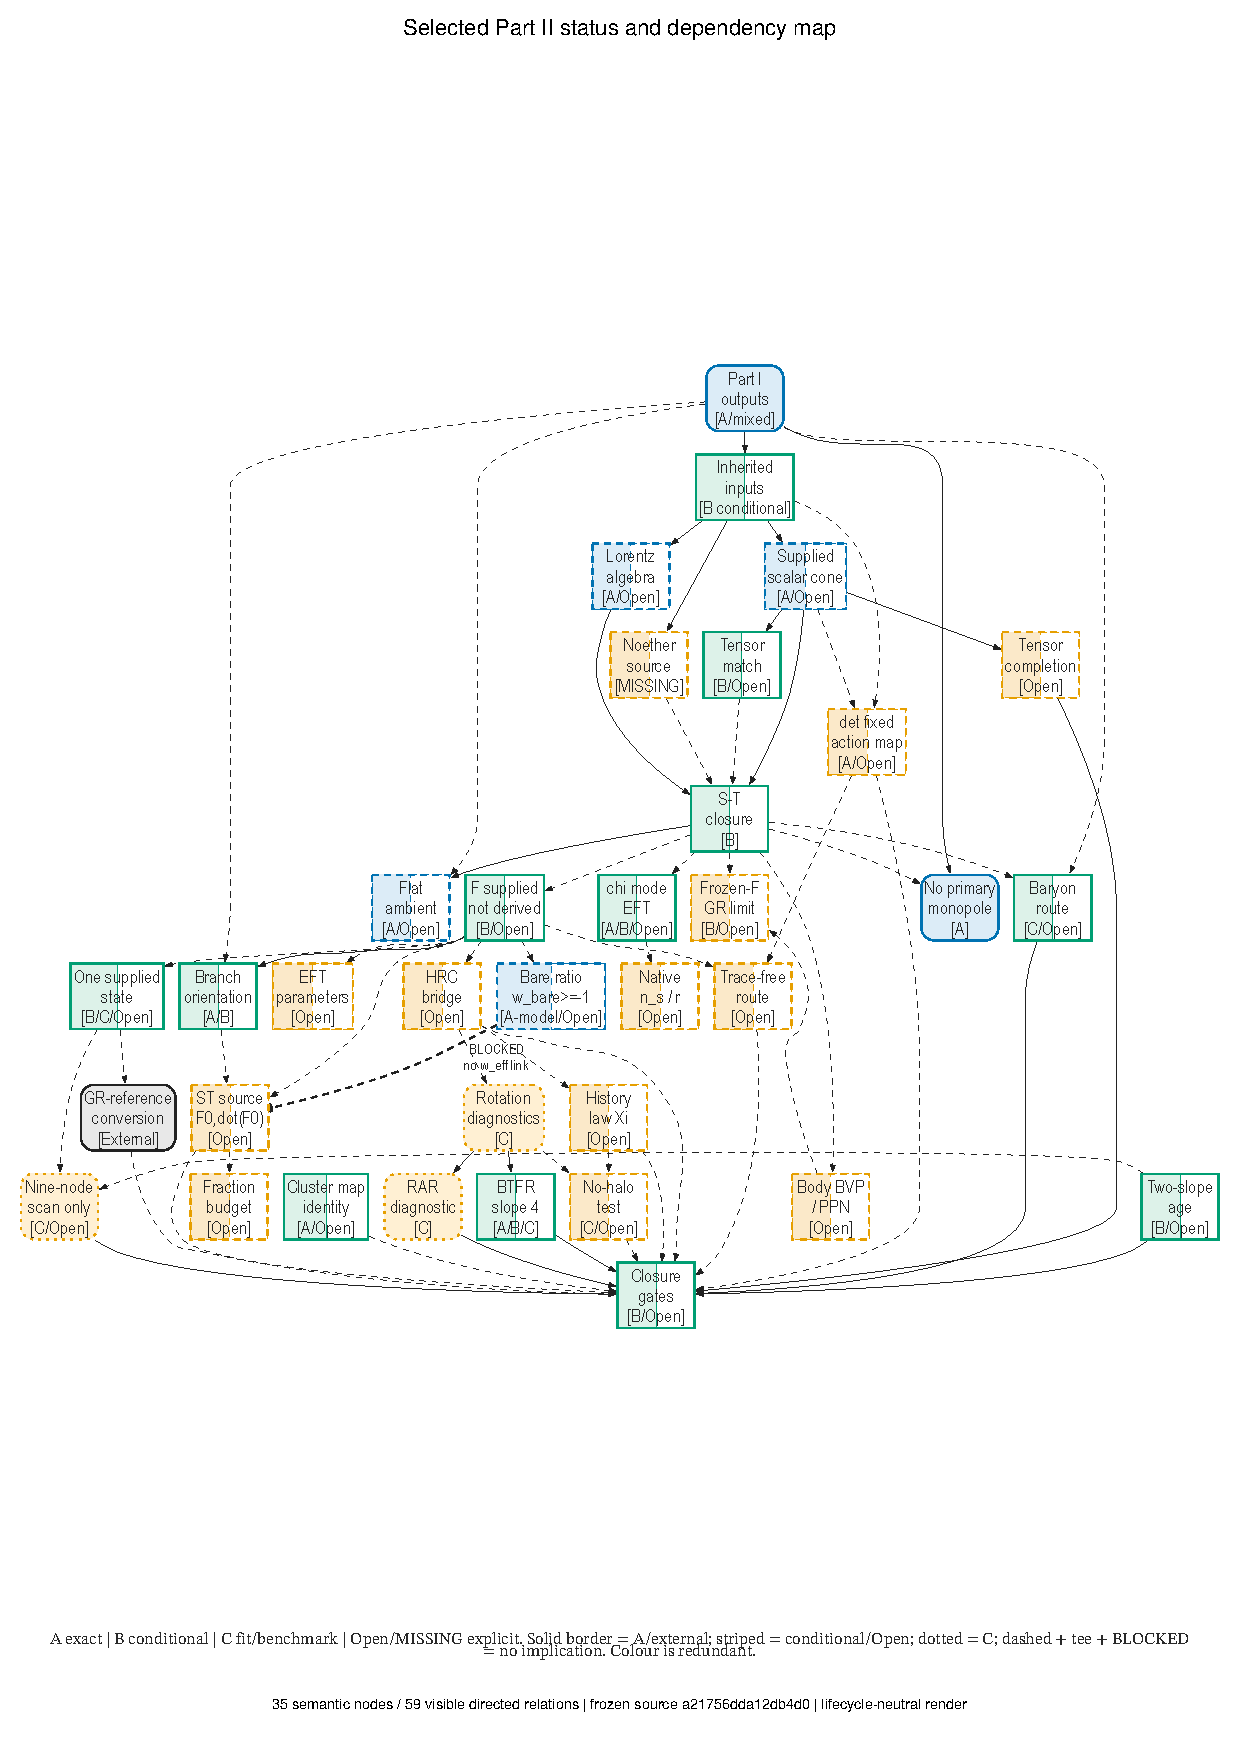
\includepdf[
  pages=1,
  pagecommand={\thispagestyle{empty}\phantomsection
    \refstepcounter{figure}
    \label{fig:partII_derivation_logic}
    \label{fig:partII_derivation_logic_A}
    \label{fig:partII_derivation_logic_B}
    \label{fig:partII_derivation_logic_C}
    \label{app:r141_complete_part_ii_logic}
    \label{app:r129_visual_part_ii_logic}
    \label{appfig:r123_topology_fig24}
    \addcontentsline{lof}{figure}{\protect\numberline{\thefigure}Selected status and dependency map of Part~II}}
]{figures/r185/logic_maps/partII_status_dependency.pdf}

\paragraph{Reading discipline.}
Solid arrows in Figure~\ref{fig:partII_derivation_logic} organise declared
dependencies; dashed arrows expose assumptions, matches and missing owners.
An arrow never upgrades a node's status.  The map's direct labels and
luminance-separated palette remain authoritative in colour and grayscale.
The repository source and machine topology retain the exact edge inventory,
which is not repeated as a reader-facing ledger.

\paragraph{Macroscopic outcome of Part~II.}
Part~II develops the macroscopic physics of ECT from the
ordered-branch inputs inherited from Part~I.
Its organising postulate-level basis is the existence of the ordered
branch itself~(P4), together with the admissibility of non-uniform and
slowly varying ordered configurations at macroscopic scales~(P6).
Within that inherited framework, Part~II develops conditional gravity
and classical-cosmology completion programmes, supplied-branch algebra,
Level-C galactic and cluster diagnostics, and a status-separated
dark-sector reinterpretation.

The strongest current outputs of the chapter are:
the distinction between ambient Euclidean flatness and the still-open
physical FLRW-curvature bridge, including a conditional planar $k=0$
proof-of-class,
the conditional $\pi_2(S^3)=0$ classification of the supplied target,
\emph{the Level~A orientation determinant identity and the distinct
conditional trace-free shift covariance}
(Section~\ref{sec:cc_problem}): fixed
$\det K^{AB}=\beta^3(\beta-\alpha)$ holds on the fixed-coefficient
orientation submanifold, but does not derive a physical constrained metric
action.  In the separately supplied trace-free completion,
$V\to V+C_0$ and $C_I\to C_I-C_0$ leave the classical equations invariant;
$C_I$ may be a measured boundary/state datum.  The ordinary two-slope
completion independently supplies a regular late-de-Sitter proof of class,
but is not shift invariant.  The physical ECT action, state, metric and
late-source map remain Open,
the dimensionally normalised bare scalar-ratio inequality inside the supplied
positive-kinetic stress (with no corresponding bound on observable $w(z)$),
the BTFR slope~$4$ as Level-A algebra inside the supplied HRC
functional and a Level-B/Open corollary after the declared gravity bridge, the Level-C matched input
$a_{M0}\approx cH_0/(2\pi)$ with microscopic origin Open, an Open
environment/history programme, and the cluster peak-preservation
identity as Level-A mathematics in the supplied monotone map, with the
physical cluster response and morphology remaining Open.
The chapter distinguishes exact equations inside declared actions,
conditional ECT ownership, exact negative constraint/stability tests,
and observable-specific Open forward models.  This status separation is
essential for interpreting every numerical claim.

\paragraph{Status-separated outputs of Part~II.}
Within the inherited ordered-branch framework, the macroscopic branch
records the following conditional statements, benchmarks, and Open
programmes:
\begin{enumerate}
  \item A controlled pure-metric gravitational branch and a
    Level-B scalar--tensor ansatz with corrected field equations.  The exact
    divided matter coefficient is $G_{\rm div}=G_*/F$; its Cavendish,
    finite-body and cosmological response maps remain Open.  The
    constant-background GR-form equation is conditional and is not by itself
    a physical GR-response limit. A covariant orientation action, any resulting
    $T^{(n)}_{\mu\nu}$, and the condensate matching of $F,K,V$ remain separate
    Open/closure inputs rather than derived functions of the displayed
    scalar-only action.

  \item A scalar signal-speed bound
    (\S\ref{subsec:sr_speed_bound}):
    the characteristic cone of the supplied scalar principal symbol
    confines disturbances of that scalar model to its closed causal cone.
    For $m\neq0$ and finite $k$, a narrow-band packet centre has
    sub-characteristic group velocity, while the front remains on the cone;
    in flat $3+1$ dimensions the massive retarded kernel has both a
    cone-boundary term and an interior tail.  In the massless flat-$3+1$
    case the retarded fundamental solution is supported on the cone.
    No physical photon, matter or tensor speed follows until its action and
    observable metric are supplied.
    The independently supplied EFT parameters $(\alpha,\beta)$ are fixed in
    the homogeneous benchmark; P4 does not derive them as vacuum-state
    parameters.  A macroscopic completion may vary candidate geometry, but
    its physical cone and matter/photon/tensor matching remain Open.

  \item P1 supplies a flat Euclidean ambient metric; a spatially flat
    physical branch is a conditional planar proof-of-class, not yet a
    derived FLRW metric.  The supplied target has $\pi_2(S^3)=0$, while a
    physical monopole/relic conclusion remains Open; one longitudinal scalar coordinate parametrises
    the stated constrained linear map; the physical one-mode reading is
    conditional.

  \item For the supplied translation-invariant strict-pullback kernel, the
    exact equal-$w$ power, sharp quartic coercivity, fixed-$k$ and full-domain
    positivity conditions, finite-deformation ratio and seed tilt, pointwise
    dominance bounds and finite-band tolerances are derived.  This is
    Level~A conditional mathematics of the displayed fixed-coefficient
    kernel.  Reflection positivity, a physical projector, coefficient
    ownership/running and the $\chi\to\zeta$ observable transfer remain Open;
    the result is not a CMB prediction.

  \item A scalar-only ordered-branch cosmological model whose equations
    are exact inside the supplied action, together with a proof that the
    unowned closure functions and state do not identify one $H(a)$.  The age
    quadrature is exact after $H(a)$ and $a_{\rm ord}$ are derived; Hubble,
    JWST, growth, ISW, lensing, clusters and PPN remain owner-specific Open
    calculations (\S\ref{sec:ect_cosmology_closure}).

  \item A conditional HRC static functional whose algebraic diagnostics
    address rotation-curve/RAR/BTFR phenomenology without a particle halo
    in that test.  Its identity bridge, action ownership, source map and
    field-level disk solution remain Open.

  \item A matched critical-scale reference
    $a_{M0}\approx cH_0/(2\pi)$ and fitted per-galaxy
    $a_{M,\rm eff}$ values; their microscopic relation and any
    environment/history law are Open.

  \item An exact theorem that any supplied strictly increasing local
    transform preserves the ordering and possibly empty set-valued argmax of
    its input baryonic field.
    No cluster-specific synthetic input or amplitude is retained; physical
    morphology, response and observational calibration are Open.

  \item A sector-by-sector inventory of external orientation proxies.
    No $\mathcal X^{\rm cand}_{\mu\nu}[n]$ contribution is derived from the scalar action;
    a covariant $S_n[g,n]$, projection, and coefficients remain Open.

  \item A dark-sector reinterpretation in which galactic mass
    discrepancy, possible coherent/topological dark sectors, and
    late-time dark energy are treated as distinct questions within the
    same condensate architecture.
\end{enumerate}

\paragraph{What Part~II inherits, what it establishes, and what
remains open.}
Part~II does not start from a blank slate.  It conditionally inherits the
P4 ordered branch and its scalar principal tensor from Part~I; the physical
metric/gravity and coherent-state sectors remain separate completion
programmes rather than inherited theorems.

Within that inherited framework, Part~II establishes the strongest
macroscopic structural outputs:
P1 provides a flat Euclidean ambient metric and a conditional planar
route to $k=0$; the physical FLRW metric remains Open.  The primary
supplied $S^3$ target has no $\pi_2$-protected map class; whether this excludes
any physical monopole channel remains Open.  The stated constrained
perturbative map contains one longitudinal scalar coordinate; a physical
one-mode sector requires the supplied reduced EFT and projector.

At the next level, the declared scalar/cosmological and galactic
closures yield conditional algebraic consequences and benchmark fits.  These
include the bare scalar-ratio inequality within the positive-kinetic ansatz
(not an observable $w_{\rm eff}$ bound), the
Hubble/JWST programme, the HRC-0/HRC-3 response construction with
its separate Open gravity bridge, the HRC-only BTFR/RAR diagnostic record,
and the cluster proxy's exact peak-preservation identity (which is not
morphology evidence).  The present scale is matching, and
environment/history dependence of the response scale is Open.

The displayed scalar action contains no independent $n_\mu$.  Accordingly,
the orientation footprint is an inventory of Level-C external proxies for a
possible future $S_n[g,n]$, not a derived beyond-benchmark layer.  This status
must remain explicit when interpreting the numerical sensitivities.

At a weaker benchmark level, specific late-time trajectories,
calibrated dark-energy reconstructions, semi-analytic maturity budgets,
and Level-C galaxy-by-galaxy fits depend on closure choices and
calibrated parameters.
Section~\ref{sec:mp_tests} organises the evidence by equation owner,
constraint/stability result and observable forward model; no attached
background is treated as a physical cosmological result.

What remains open is the primordial spectrum ($n_s$, $r$),
the cosmological fraction budget, the full nonlinear $\phi$
boundary-value problem, and the detailed ontology of coherent
dark-sector excitations.


\begin{longtable}{@{}L{3.20cm}L{3.70cm}L{4.40cm}L{3.20cm}@{}}
\caption{Numerical inputs, conditional outputs, external anchors, and fit
diagnostics of Part~II.
The entries are not all of the same logical type:
some are conditional algebra, some are closure-level benchmark estimates,
some are external constraints, and some are comparative fit diagnostics.
The final column records this status explicitly.}
\label{tab:partII_numerical}\\
\toprule
Item & Value / conditional output & Observation / comparison & Status \\
\midrule
\endfirsthead
\toprule
Item & Value / output & Obs./comp. & Status \\
\midrule
\endhead
\bottomrule
\endfoot
BTFR slope & $4$ for either HRC deep branch after the gravity bridge & $3.98\pm0.08$ & B / bridge Open \\
$a_{M0}$ (matched HRC gravity scale) & $cH_0/(2\pi)=1.08\times10^{-10}$\,m/s$^2$
  & $a_0\approx1.2\times10^{-10}$ (McGaugh) & Matching; ECT origin Open \\
MW representative disk sensitivity & HRC-0: $\chi^2_\nu=1.813$, $a_M/a_{M0}=2.798$
  & HRC-3: $\chi^2_\nu=2.287$, $a_M/a_{M0}=1.703$
  & Level~C; not a modern Milky-Way posterior \\
$n_s,A_s,r$ (primordial spectrum) & Supplied pure-quartic strict-pullback kernel gives local $n_\chi=1$ exactly when its combined $\kappa_\chi$--kernel normalisation is scale-independent (separate constants suffice); exact finite-band bounds depend on $\delta_a,\delta_m,\rho$; physical mass, measure/state/projector and complete transfer open & CMB scalar/tensor targets: $n_s\!\simeq\!0.965$, $A_s$ obs., $r$ bounded & A-math conditional / B/Open physical \\
$\eta_B$ (baryon asymmetry) & No ECT value
  & External target from a named Planck base-$\Lambda$CDM fit plus standard
    conversion~\cite{Planck2018} & Open; physical current, vertex, state and
    transport absent \\
GW--EM relative speed & Open: no ECT value & Joint interval $[-3,+0.7]\times10^{-15}$~\cite{LIGO_Fermi_GW170817_GRB2017} & External gate \\
Late-time expansion history & Named near-GR two-slope orbit; official
  15-point BC03 chronometer calibration gives
  $H_0=68.59\pm3.95$ km\,s$^{-1}$\,Mpc$^{-1}$
  & BAO, supernovae, chronometers and growth data
  & Level~C calibration; owner-complete joint likelihood Open \\
ECT cosmological background and age & Named two-slope scalar--tensor action/state:
  $H_{2s}(0)\Delta t=0.9636868$ and covariance-calibrated
  $t_0=13.74\pm0.79$~Gyr conditionally
  & Exact owner audit (\S\ref{sec:ect_cosmology_closure})
  & Level~A within the named completion; dimensional scale calibration Level~C;
    P1--P6 ownership Open \\
\end{longtable}

\paragraph{Bridge to Part~III.}
With the macroscopic branch in place, the next task is to return to the
coherent and quantum structure of the condensate.
Part~III develops the coherent branch across eleven thematic steps:
the action-scale and winding programme, wave kinematics and
conservation laws, the Hilbert-space bridge through reflection
positivity and unitarity, exchange-sector topology and Dirac structure,
the unified vacuum-response programme, decoherence and the arrow of
time, the quantum--classical boundary and Born-type probability,
entanglement, the wider topological/dark-sector ontology, black-hole
thermodynamics and the information-exclusion result, and the
analogue source-model comparison and bridge-building programme.

\paragraph{Conceptual output: scalar characteristic-metric notation.}
ECT takes the $\Phi$-medium, rather than a physical metric, as the primitive
model entity.  In the supplied scalar EFT it is convenient to denote the
inverse principal tensor by ``characteristic metric'' because it records the
propagation characteristics of that scalar operator.  This notation is not a
derivation of a universal observable metric.  A possible gravity completion
may be a long-wavelength condensate response, but the fixed director map has no
linear transverse--traceless/static-density vertex; physical rods, clocks,
photons, matter and nonlinear gravity require separate owners.
Two further foundational issues find natural homes in the macroscopic
branch: the primary condensate vacuum satisfies $V''(\phi_0)>0$ at
tree level, while the strict one-real-scalar one-loop running has
$\beta_\lambda>0$ and therefore excludes only the Standard-Model-like
negative-running route at that order
(\S\ref{par:vacuum_stability_oneloop}; Level~B conditional).  Full
effective-potential, branch-architecture and embedded-sector stability remain
Open~\cite{Degrassi2012,Buttazzo2013};
\S\ref{sec:radial_mode}); and the duration and relative density of any late-time source are not
identified until one globally regular background, physical metric and
state are derived.  The cosmological-coincidence question therefore
remains an Open dynamical problem;
this is logically separate from the conditional trace-free vacuum-offset completion and its still-Open $\Phi$-medium action descent (Section~\ref{sec:cc_problem}).




%%% -----------------------------------------------------------

% ==============================================================
\subsection{Global Level-4 self-consistency checklist}
\label{sec:global_level4_checklist}
% ==============================================================

\paragraph{Role of the checklist.}
The present table is not a second derivation map and not a duplicate of the
status-separated claim inventory.
Its purpose is different: it provides a compact Level-4 audit of the
framework as a whole, combining inherited consistency conditions from
Part~I, macroscopic results from Part~II, and deferred or open items that
extend into the Quantum Sector.
It should therefore be read as a global status board rather than as a
local summary of Section~\ref{sec:mp_conclusions} alone.

\paragraph{Postulate-level organisation.}
At the structural level, the checklist probes four layers of the ECT
architecture:
the microscopic consistency of the Euclidean $\Phi$-medium (P1--P3),
the ordered macroscopic branch and its admissible non-uniform
developments (P4--P6),
the coherent sector (BR1, S10),
and the still-open bridges required to close the full framework.
The \textsc{pass} / \textsc{part.} / \textsc{prob.} / \textsc{open}
labels should be interpreted in that same layered sense.
Unlike the derivation map, which records logical dependencies, and unlike
the falsifier table, which records observational tests, the present
checklist answers a different question: which framework-level consistency
targets are already passed, only partially controlled, structurally
motivated but not rigorous, or still open.

\paragraph{Architectural completions from the emergent matter-sector
trilogy.}
The discrete-symmetry architecture~(\S\ref{sec:discrete_symmetries}),
the anomaly architecture~(\S\ref{sec:anomaly_architecture}), and the
flavour architecture~(\S\ref{sec:flavour_architecture}) now provide an
explicit conditional consistency audit for a supplied chiral gauge completion.
Their Level-4 audit status is therefore recorded in the checklist
below alongside the original whole-framework consistency items.

\medskip\noindent
\textit{Scope legend:} I~= inherited from Part~I (foundations);
II~= macroscopic branch of Part~II;
III~= Quantum Sector / Part~III;
G~= global whole-framework closure problem.

\begingroup
\setlength{\tabcolsep}{6pt}
\renewcommand{\arraystretch}{1.25}
\small
\begin{longtable}{@{}L{1.4cm}L{1.4cm}L{3.5cm}L{6.6cm}L{1.4cm}@{}}
\caption{Level-4 self-consistency checklist.
\textsc{pass} = a named mathematical/source-model test reproduced under its
displayed assumptions, not automatic physical ECT closure;
\textsc{part.} = a partial conditional calculation with its missing owners declared;
\textsc{prob.} = structurally motivated, rigorous proof pending;
\textsc{open} = known open problem.}
\label{tab:level4_checklist}\\
\toprule
\textbf{Status} & \textbf{Scope} & \textbf{Check} & \textbf{Outcome} & \textbf{Ref.} \\
\midrule
\endfirsthead
\toprule
\textbf{Status} & \textbf{Scope} & \textbf{Check} & \textbf{Outcome} & \textbf{Ref.} \\
\midrule
\endhead
\bottomrule
\endfoot
\textsc{part.} & I & Condensate stability      & Tree-level local stability plus a positive-running check in the strict one-loop scalar truncation; full effective-potential and branch-architecture stability remain open                                   & \S\ref{par:vacuum_stability_oneloop}, \S\ref{sec:ssb} \\
\textsc{part.} & I & Quadratic stability of supplied scalar closure & Kinetic/gradient signs are healthy only after the supplied $\alpha>\beta>0$ component, $\varsigma_L=-1$ orientation and $A_{L,\varphi}>0$; full non-negativity is the declared spectral/domain test, whose stationary P4 owner remains Open & \S\ref{sec:ssb} \\
\textsc{open} & I & Physical tensor/ghost test & No linear TT/static-density seed at fixed $\alpha,\beta$ and tangent-director order; quadratic response is parametric and a constrained tensor Hessian/residues remain missing & \S\ref{sec:graviton} \\\
\textsc{open} & G & Full non-perturbative ghost-freedom and exact TT closure of a candidate physical graviton completion & Completion-level question tied to gauge/gravity closure (OP3) & \S\ref{sec:graviton}, \S\ref{sec:open_problems} \\
\textsc{open} & I & Tensor propagation gate & $c_{\rm GW}$ and tensor LIV operators are not identified; GW170817 is an external completion test for a future action & \S\ref{sec:mp_gw} \\\
\textsc{part.} & I & Discrete-symmetry architecture of emergent matter sector & Euclidean reflection identities are A-math; their physical P/T identification, OS/CPT reconstruction and completed matter action are conditional/Open; $\mathcal{L}_5$ is only a candidate preferred-background operator & \S\ref{sec:discrete_symmetries} \\
\textsc{open} & I & Anomaly audit for a supplied chiral gauge completion & Standard anomaly equations and arithmetic are A conditional on supplied representations; $\mathcal{L}_5$ is representation-data transparent; the physical local bundle, chirality and matter spectrum are Open (OP-GUT6 family) & \S\ref{sec:anomaly_architecture} \\
\textsc{open} & G & Flavour architecture (CKM/PMNS) & Basis-misalignment algebra is standard; overlap profiles, generations, representations, Yukawa matrices, CKM/PMNS entries and phases require supplied spectral/matter closures & \S\ref{sec:flavour_architecture} \\
\textsc{pass} & I & Scalar-operator causality test & Retarded propagation for the supplied hyperbolic scalar operator; positive pairwise noise quadratic only in a declared Gaussian source model, with physical matter/photon/tensor cones and the ECT record kernel Open & \S\ref{sec:arrow_of_time} \\
\textsc{open}& G & ECT entropy-production theorem  & Ohmicity/Markovianity and positive pairwise noise are insufficient; reduced channel, state, entropy functional, and unitality/detailed-balance/contractivity hypotheses required (OP-Q17) & \S\ref{sec:second_law_basics} \\
\textsc{open}& III & Born measure              & A complete applicable corrected OS-II package for a supplied Gaussian model reconstructs a positive quadratic norm.  Independently, ordinary projector Gleason represents a supplied normalised, noncontextual, countably additive projector measure only for a complex Hilbert space with $\dim\mathcal H\ge3$; a qubit requires the Busch effect/POVM theorem under separately declared C2q hypotheses.  State/preparation, event, probability origin, outcome and update remain Open & \S\ref{sec:born_rule} \\
\textsc{open}& II & Primordial perturbations $n_s$, $r$ & The strict map has one scalar coordinate (A kinematics); a supplied reduced EFT may promote it to one physical mode (B).  The curvature variable, state, transfer and CMB likelihood are Open.  A conditional Lifshitz window is not a prediction of $n_s$ or $r$ & \S\ref{sec:mp_cosmo} \\
\textsc{open}& II & Baryogenesis              & A supplied transition/matter completion may host Sakharov ingredients; no ECT value of $\eta_B$ is calculated (OP7)            & \S\ref{sec:baryogenesis} \\
\textsc{cond.} & III & Unruh temperature         & Standard Rindler/KMS result only after a Lorentzian QFT state, detector coupling, analyticity and $S_0=\hbar$ matching are supplied; ECT owner Open & \S\ref{sec:unruh} \\
\textsc{cond.} & III & Orientation-sector Casimir (ideal boundaries) & Idealised boundary-value calculation; whether matter imposes those boundaries and the force magnitude/sign are Open & \S\ref{sec:casimir} \\
\textsc{open} & III & Casimir: lab applicability & Material boundaries $\to$ soft orientation sector: not derived & \S\ref{sec:casimir} \\
\textsc{open} & II & Tensor ratio $r$ & ECT-native derivation pending; removed borrowed slow-roll formula & \S\ref{sec:mp_cosmo} \\
\textsc{open}& G & Renormalisability         & A scalar EFT on a fixed background does not establish UV safety of a physical tensor/gauge/matter completion; its action, constraints and counterterms are missing & \S\ref{sec:open_problems} \\
\textsc{open}& G & 3 fermion generations     & Three-state counts occur only in supplied spectral wells with parameter/boundary choices; physical generations, representations, masses and mixings are not derived & \S\ref{sec:yukawa}, \S\ref{sec:flavour_architecture} \\
\textsc{open}& G & $\alpha_{\rm fs}$; SU(3)  & The identity
$\alpha_{\rm fs}=q^2/(4\pi Z_A)$ is conditional on a supplied physical gauge
normalisation; ECT derives neither the electroweak owners nor the colour
sector (\S\ref{sec:alpha_fs}) & \S\ref{sec:alpha_fs} \\
\textsc{cond.}& II & Cosmological background and age & One supplied two-slope action/state gives conditional $H(z)$, distances and ages after one declared calibration; the official 15-point BC03 covariance gives $H_0=68.59\pm3.95$ and $t_0=13.74\pm0.79$~Gyr for that orbit.  The microscopic completion and physical clock/metric map, not the legitimacy of state data, remain Open & \S\ref{sec:two_slope_background_proof_class}, \S\ref{sec:ect_cosmology_closure} \\
\textsc{open}& II & JWST early-object forward model & Conditional clock and hybrid rare-peak sensitivities are computed; abundance and morphology still require perturbations, halo/baryonic modelling and survey selection & \S\ref{sec:mp_tests} \\
\textsc{part.}& II & Force-law dimensionality diagnostic & $d_{\rm force}(x)$ crossover $3\to 7/3\to 2$ algebraic for the HRC-0 shape; no retroactive action derivation & \S\ref{sec:universe_size} \\
\textsc{open}& II & Environment/history dependence of $a_{M,\rm eff}$ & An exploratory factor $\Xi$ is defined for cross-correlation tests; its microscopic map, sign, amplitude, and density-only closure are Open & \S\ref{sec:mp_galactic_phenom}, \S\ref{sec:dark_discriminants} \\
\textsc{cond.}& II & HRC constitutive response & HRC-0 exact in the augmented ERP-$\Phi$/inverse-DtN model; HRC-3 conditional in the supplied three-channel model; gravity bridge and P1--P6 ownership Open & \S\ref{sec:hrc_erp_candidate} \\
\textsc{cond.}& II & Galactic dark-sector benchmark & HRC is the active candidate; HRC-only algebraic fit outputs are Level-C diagnostics, not predictions; cosmological fraction budget Open & \S\ref{sec:dark_matter_interp} \\
\textsc{open}& II & Cluster projected-proxy sanity audit & Strictly local $\nu_{\rm cl}$ transform preserves every positive baryonic-pixel ordering exactly; no morphology evidence; action/source/lensing response and observational calibration Open & \S\ref{sec:bullet_cluster}, \S\ref{sec:dark_discriminants} \\
\textsc{open}& II & Varying-constants protection (OP-CONST) & Selective-coupling and frozen-background constructions are conditional routes only; the physical matter map and microscopic protection theorem remain Open & \S\ref{sec:ect_cosmology_closure} \\
\end{longtable}
\endgroup

% ==============================================================
\subsection{Global dependency, status, and completion-test maps}
\label{sec:global_maps}
% ==============================================================

\paragraph{Role of the global maps.}
The following tables provide three complementary global views of the
ECT programme.
Table~\ref{tab:ect_structure} records the logical status and dependency
architecture:
which sectors depend on which earlier inputs and closure assumptions.
Table~\ref{tab:ect-levels} records the epistemic status of those outputs
in the Level~A / Level~B / Open discipline adopted throughout the paper.
Table~\ref{tab:ECT_predictions} records conditional calculations, external
constraints and Open completion tests.  An Open row is not a present ECT
signature or falsifier.
These three maps should therefore not be read as redundant summaries,
but as answers to three different questions:
what follows from what,
how strongly it is established,
and how it can fail.

\paragraph{Postulate-level organisation.}
At the highest structural level, all three maps are organised by the
same postulate hierarchy:
the microscopic Euclidean $\Phi$-medium and its consistency conditions
(P1--P3),
the ordered macroscopic branch and its admissible non-uniform
developments (P4--P6),
and the coherent sector (BR1, S10) whose full ontology is
taken up later in the Quantum Sector.

The narrative conclusions of Part~II were summarised in
Section~\ref{sec:partII_conclusions}, while the audit-style checklist was
given in Section~\ref{sec:global_level4_checklist}.
The tables below complement those layers by presenting the same framework as
a status-and-dependency map, a status map, and a completion-test map.
Entries should be read against the same layered vocabulary used in the
final status board~(Section~\ref{sec:mp_status}): inherited structural
inputs, closure-level outputs within the present $\phi$-first
programme, benchmark/calibrated implementations, and open problems.
For the macroscopic branch developed in Part~II, the declared near-term
test is the prespecified environment/history regression~(F1).  The
bare scalar-ratio identity~(F5) is a conditional internal check rather than an
observable bound or ECT prediction.  A physical cluster-lensing test~(F10) remains
Open; the current local proxy is not a discriminant.

\begin{longtable}{@{}L{3.4cm}L{8.2cm}L{2.9cm}@{}}
\caption{Status and dependency map of ECT: physical objects and their
declared inputs or owners in the Level~A / Level~B / Open discipline.
Entries: ``derived'' denotes Level~A, exact in the declared model and
assumptions, with an explicit reproducible derivation; reproducible checks verify that derivation but do not replace it; it does not by itself
establish descent from P1--P6 or physical ECT ownership.  ``Structural /
effective (Level~A/B)'' means proven in the pure-metric limit and Level~B in
the $\phi$-first closure; ``matched (Level~B)'' denotes an EFT matching
relation; ``embedded'' means introduced consistently, not derived from the
bare scalar action; ``open'' denotes an active research direction.} \\
\label{tab:ect_structure} \\[-6pt]
\toprule
\textbf{Object} & \textbf{Origin in ECT} & \textbf{Status} \\
\midrule
\endfirsthead
\toprule
\textbf{Object} & \textbf{Origin in ECT} & \textbf{Status} \\
\midrule
\endhead
\midrule\multicolumn{2}{r}{\small\textit{(continued on next page)}}\\
\endfoot
\bottomrule
\endlastfoot
4D Euclidean space & Postulate P1 & postulate \\
$O(4)$ symmetry & Postulate P2 & postulate \\
Condensate field $\Phi$ & Postulate P3 & postulate \\
Ordered-gradient physical sector & Postulate P4 & postulate; stationary owner Open \\
Scalar characteristic-metric candidate & Supplied P4 branch and scalar principal tensor with $\beta(\beta-\alpha)<0$; healthy shorthand $\alpha>\beta>0$ only for $\beta>0$ & conditional A-math; universal physical metric Open \\
Physical/\allowbreak thermodynamic arrow of time & Retarded support in a supplied scalar problem and dephasing in a supplied reduced channel are insufficient & Open: state, map, entropy functional and contractivity/\allowbreak detailed-balance owner required \\
Scalar common-length slope $\hat c_*$ &
$\hat c_*=\sqrt{\beta/(\alpha-\beta)}$ from the supplied scalar principal
tensor & A-math conditional \\
Dimensionful scalar speed $c_{\rm char}$ &
$c_{\rm char}=c_{\rm u}\hat c_*/\mathcal N_\Phi$ after a supplied
clock, conversion speed and lapse & $c_{\rm char}=c$ adopted Level~B
calibration; photon/tensor cone equality Open \\
Gravitational coupling $G_N$ & Geometric EFT matching: $G_N^{\rm nat}=(8\pi M_G^2)^{-1}$ & matched (Level~B) \\
Ordered-branch amplitude variable $\phi$ & Macroscopic closure variable for slow amplitude variations of the ordered branch & effective (Level~B) \\
Pre-quantum action scales & The phase-only fixed-core model defines $\iota_0^{\rm EFT}$ after $L_{\rm core}$ is supplied; the optional tension-balanced model defines the distinct $\iota_{0,\rm bal}^{\rm eff}=\sqrt{2K_\theta^{1\mathrm D}\mathcal T_{\rm loop}}$.  CDE-$\Phi$ is only a post-order acceptance criterion; the actual owner must be one explicit 4D action, state, profile, subtraction and physical quotient & A mathematics for the supplied bounds/minimum / Level-B generic-EFT route / carrier, compact modulus and ECT ownership Open \\
Operational action unit and physical reduced Planck constant & Candidate owner maps $\Sigma_\theta\iota_0^{\rm EFT}$ or $\Sigma_\theta\iota_{0,\rm bal}^{\rm eff}\to S_0$, followed separately by the Level-B calibration $S_0=\hbar$ & Calibration adopted conditionally; physical owner, absolute derivation and universality remain Open and are not identified by the present action \\
Schr\"odinger-type equation & Supplied norm-preserving complex sector, Hamiltonian, domain, clock and NR limit & conditional algebra; ECT owner B/Open \\
Macroscopic scalar closure & Pure-metric conditional limit + Level-B $\phi_u$ ansatz; galactic functional separate & A/B; S$\to$G Open \\
Physical graviton & $h_{ij}^{\rm TT}=h_{ww}=0$ only at fixed $\alpha,\beta$ and tangent-director linear order about homogeneous $n=w$; quadratic/nonlinear routes remain parametric/Open; Fierz--Pauli supplied & A-math conditional negative result / Open physical spin-2 completion \\\
Photon & Compact phase gives global Noether algebra; a local bundle/connection, unbroken transverse photon, charge/matter map and metric require completion & conditional route / Open \\
$W^\pm,Z^0$ & Supplied electroweak doublet and chiral gauge completion & embedded model-building / Open descent \\
Higgs-like boson & Radial mode of the secondary electroweak condensate doublet & structural / phenomenological matching (Level~B+) \\
Fermions & Supplied spinor/CAR fields on the ordered background & conditional/Open physical origin \\
Neutrino sector & No physical chiral/mass operator derived; weak-sector,
  PMNS/MSW and seesaw closures may be supplied; the geometric-scale
  expression is an unselected historical ansatz only & C/Open \\
Late-time acceleration source & Regular two-slope proof of class plus a distinct conditional trace-free $C_I$ branch; physical ECT source, state and observable map Open & A in supplied actions / C benchmark / Open ECT \\
Dark-sector role & No particle halo in the Level-C HRC algebraic diagnostic; particle content and cosmological fractions Open & C/Open \\
Flat rotation curves and RAR/BTFR phenomenology & HRC-0/HRC-3 augmented-model response plus separate gravity bridge; HRC algebraic diagnostics recomputed & A/B/C by layer / live ECT Open \\
Macroscopic entropy theorem & Conditional reduced-channel result only after the map, state, entropy functional, and contractivity/detailed-balance hypotheses are declared & Open for ECT \\
Universal causal cone & One scalar characteristic cone only; gauge, fermion, matter and tensor cones require independent owners & Open beyond scalar subsector \\
LV suppression & Higher-dimensional-operator benchmark, with coefficients and sector maps unspecified & conditional EFT benchmark \\
Proton stability & Three selection-rule patterns conditional on gauge/flavour completion (\S\ref{sec:proton_stability}) & conditional (Level~C) \\
Vacuum-offset and late-source status & The orientation determinant is
fixed only on its stated submanifold and does not derive a metric action.  An
explicit trace-free completion is shift covariant through $V+C_I$; a separate
ordinary two-slope completion is regular but not shift invariant.  The ECT
action descent, physical metric and state-to-observable map are Open &
orientation algebra A; supplied completions A; ECT descent B/Open; calibrated
late history C \\
\hline

\end{longtable}


\begingroup
\setlength{\tabcolsep}{3pt}
\begin{longtable}{@{}L{0.055\textwidth}L{0.295\textwidth}L{0.135\textwidth}L{0.330\textwidth}L{0.100\textwidth}@{}}
\caption{Structured classification of ECT statements, benchmarks, and Open
targets.  Level~A = exact in the
declared model and assumptions, with an explicit reproducible derivation; reproducible checks verify that derivation but do not replace it; it
does not by itself establish descent from P1--P6 or physical ECT ownership.
Level~B = structural/conditional derivation or closure route with a
declared open matching, input, or identification step; Level C = phenomenological fit,
benchmark, or candidate mechanism; Open = missing/unidentified input or future
programme.}
\label{tab:ect-levels}\\
\toprule
\# & Statement & Level & Declared model / assumptions / owner & Section \\
\midrule
\endfirsthead
\toprule
\# & Statement & Level & Declared model / assumptions / owner & Section \\
\midrule
\endhead
D1 & Supplied scalar principal tensor is Lorentzian iff $\beta(\beta-\alpha)<0$; on the healthy $\beta>0$ branch this is $\alpha>\beta>0$; realised branch selection is Open & A-math conditional / Open & P4 does not determine the sign of $\beta-\alpha$ or the physical vacuum/clock/metric & \ref{sec:ssb} \\
D2 & KG form and mass map from the supplied scalar operator plus the declared clock/lapse map; Schr\"odinger limit only after an additional rest-energy/low-momentum reduction & \textbf{A-math conditional / B--Open} & The KG algebra uses no Osterwalder--Schrader continuation; the P4 action, mass/domain matching and physical-mode ownership remain Open & \ref{sec:ssb},\,\ref{sec:qs_wave} \\
D3 & $G_N$ from geometric EFT matching ($G_N^{\rm nat}=(8\pi M_G^2)^{-1}$) & B & Matching between ordered-branch tensor EFT and observed gravity; explicit $(u_0,\alpha,\beta)\to M_G$ derivation open~(OP2, OP3) & \ref{sec:mp_matching} \\
D4a & A supplied nonzero P4 vector has stabiliser $O(3)$ and abstract
orbit $O(4)/O(3)\simeq S^3$; physical SSB and vacuum-manifold
identification are Open & A-math conditional / Open
& Group orbit only; P4 is not a stationary vacuum owner
& \ref{sec:sector_map} \\
D4b & $Q_A=\partial_A\Phi$ implies integrability; $\pi_i=\partial_i\chi/u_0$ & A & Scalar-only basis & App.\ \ref{app:goldstone_integrability} \\
D4c & One physical longitudinal scalar mode $\chi$ in a supplied reduced EFT & B & Requires the kinematic reduction plus action, quotient/domain and projector & App.\ \ref{app:goldstone_integrability} \\
D4d & Minimal 3-component orientation EFT & B & Effective parametrisation & \ref{sec:goldstone_soft_eft} \\
D4e & Three independent physical Goldstone particles & Open / excluded in current scalar basis & Scalar integrability leaves one longitudinal coordinate in the strict map; a larger physical bundle is not derived & \ref{sec:goldstone_integrability_main} \\
D5a & Fixed director-map tensor test: $h_{ij}^{\rm TT}=h_{ww}=0$ & A negative result / physical graviton Open & Fixed $\alpha,\beta$ and tangent director perturbation & 8 \\
D5b & Fierz--Pauli form, TT projection, ghost-free counting at linearised level & B & TT gauge; explicit mode-counting from microscopic condensate variables open (OP3 partially resolved) & 8, App.\ \ref{app:GN_derivation} \\
D6 & Dirac form (structural reconstruction once spinorial fields admitted) & B/Open & $\mathrm{Spin}(3)$ representation after restricting to the connected $SO(3)$ stabiliser; its physical-rotation and fermion owners are Open; not from the bare bosonic action & \ref{sec:fermions}, \ref{sec:dirac_eq} \\
D7 & Derrick scaling in the separately supplied two-derivative
$S^3$ sigma-model target & A-math within supplied model / physical sector and mass Open &
Target-space and action assumption; ECT configuration owner,
stabilisation, profile and mass remain Open &
\ref{sec:predicted_states} \\
D8 & Thermodynamic entropy-production programme & Open & Retarded response and positive pairwise noise do not imply monotone von Neumann entropy; derive the reduced channel, entropy functional, and detailed-balance/contractivity hypotheses (OP-Q17) & \ref{sec:second_law_basics} \\
D9 & Physical identification of an action-scale candidate with $\hbar$ & Level~B matching / Open owner & The supplied fixed-core and tension-balanced models define distinct candidates, related by Eq.~\eqref{eq:S0_bal_fixed_relation} only in the elementary sector when $L_{\rm core}=L_{*,1}$.  CDE-$\Phi$ is an acceptance criterion, not an owner or carrier.  The calibration $S_0=\hbar$ is explicit; the profile, compact modulus, cross-sector normalisation and operational owner map remain Open~(OP-Q1/OP-Q2) & \ref{sec:hbar_status}, \ref{sec:qs_hbar}, \ref{sec:qs_ccr} \\
D10 & Linearised scalar/metric equation; orientation extension separate & B/Open & Scalar closure conditional; covariant $S_n$ and its stress missing & \ref{sec:macroscopic} \\
D11 & Primordial perturbation inventory: one scalar coordinate in the strict map & A kinematics / B physical EFT & Universality Corollary supplies the coordinate reduction; action, physical mode projector, state, $n_s$ and $r$ remain open (OP3) & \ref{sec:mp_primordial} \\
D12 & Baryogenesis completion inventory & Open & P4 supplies an ordered-gradient chart, not a derived real-time transition; baryon current/violation, CP coefficient, state, transport and washout are missing, and no ECT value of $\eta_B$ is calculated (OP7) & \ref{sec:mp_baryogenesis} \\
D13 & Physical tensor-sector quantisation and UV closure & Open & The orientation/effective-metric sector is a structural candidate, but physical constraints, canonical normalisation, interacting RP/OS reconstruction, and cross-sector action-scale comparison are missing; PES-R is not a quantisation mechanism & 8, \ref{sec:open_problems}, \ref{sec:pes} \\

Q-PES & PES-R response--persistence taxonomy & B/Open & Sector dynamics first; then finite-time retention and pairwise records; topology only where owned.  Same-channel Wightman/KMS tests and primordial record-kernel constraints remain Open until physical operators, states, common filters and transfer maps are derived & \ref{sec:pes}, \ref{sec:pes_open}, App.~\ref{app:AP6A-same-channel-fdt} \\

D14 & Corrected scalar--tensor IR closure; candidate anisotropic tensor proxy & B/Open & Scalar variation exact in the ansatz; the projected-Riemann identity is false and orientation action/projection remain Open & \ref{sec:macroscopic}, App.~\ref{app:curvature_coupling} \\
D15a & Retarded support $K(\tau\!<\!0)\!=\!0$ for the supplied scalar operator after an initial--boundary orientation & A-math conditional & Quadratic pole proof plus symmetric-hyperbolic reduction; physical time/arrow Open & \ref{sec:arrow_of_time}, \ref{app:retarded_kernel}, \ref{app:causal_hyperbolic} \\
D15b & Open-system identification of bath response kernel / pre-branch origin of causal selection & C & Retarded ordered-branch dynamics provides the structural basis; full identification from Euclidean microdynamics not yet complete & \ref{sec:second_law_basics}, \ref{sec:open_problems} \\
D16a & Compact phase and local $U(1)$ completion
  & A global / Open local & Winding is exact; bundle, reduced Hessian, photon and matter map are Open
  & \ref{sec:u1_emergence} \\
D16b & Weak algebra and physical chiral $SU(2)$ sector
  & A algebra / Open physical & $\mathfrak{so}(3)\simeq\mathfrak{su}(2)$ and $SU(2)_{\rm diag}$ stabiliser are exact; no chiral factor is selected
  & \ref{sec:nonabelian_embedding}, \ref{sec:chirality} \\
D16c & $SU(3)_c$ colour sector
  & P7 Level-B / A conditional / physical Open & Direct injective embedding is
    excluded by dimension; P7 is the adopted structural bundle and its
    $SU(3)$ frame reduction is exact conditional mathematics, while physical
    colour and alternative microscopic origins remain Open.  Anomaly
    cancellation does not select
    the colour rank ($N_c$ odd only,
    \S\ref{sec:anomaly_architecture})
  & \ref{sec:colour_completion} \\
D16d & Neutrino-sector completion
  & C/Open & Physical chirality, sterile content, mass operator and PMNS
    matrix are not derived; the historical geometric-scale expression is
    unselected, and no numerical $c_L$ coefficient is retained.  The
    $a_L/c_L$ propagation algebra is conditional
    on flavour Hermiticity, identity projection, perturbative coefficients, a
    self-adjoint spatial domain and norm-bounded positive-nonsingular time
    kinetic form in the declared broken-phase constant-coefficient vacuum/free
    domain; $C=-c_L^{\mu\nu}\widehat p_\mu\widehat
    p_\nu$ for the displayed minus-sign derivative operator, and
    antineutrinos use the declared CPT conjugations
  & \ref{sec:neutrino_particles} \\
D17 & ECT entropy-production theorem & Open & Retarded support and a positive pairwise noise kernel do not fix entropy sign; derive the reduced map, state, entropy functional, and contractivity/detailed-balance conditions (OP-Q17) & \ref{sec:second_law_basics}, \ref{sec:open_problems} \\
D18 & Physical ordered-domain size & Open & No inequality relative to the
Hubble radius follows without a formation history, boundary dynamics and
physical metric/clock map (OP3) & \ref{sec:universe_size} \\
D19 & Conditional reduced loop coefficients and physical action
normalisation in the $U(1)$-extended EFT & A/B/Open & The fixed-length
Cauchy--Schwarz bound and minimum of the supplied positive-tension 1D
functional are exact dimensionless mathematics.  The $d^3y$ coefficient has
the geometry of a codimension-three worldline reduction, not an ordinary
spatial vortex worldsheet.  CDE-$\Phi$ is an acceptance criterion; only an
explicit 4D action/\allowbreak state/\allowbreak profile/\allowbreak
subtraction/\allowbreak quotient can own the route.  A physical action
requires $\Sigma_\vartheta\mathcal I_n$; in the bending-free $n=1$ branch the
Level-B calibration is
$\Sigma_\vartheta\mathcal I_{1,\min}=2\pi\hbar=h_{\rm P}$.
Carrier, compact modulus, ensemble, profile, stability,
$\Sigma_\vartheta$, its possible equality to $\Sigma_\theta$, and
universality remain Open; the distinct dimensionless coefficients
$\iota_0^{\rm EFT}$, $\iota_{0,\rm bal}^{\rm eff}$ and
$\iota_{0,\rm bal}^{(\vartheta)}$ are not interchangeable &
\ref{sec:hbar_status}, \ref{app:Sloop_calc} \\
D20 & Supplied scalar slope and physical scalar-clock calibration
$\hat c_*=\sqrt{\beta/(\alpha-\beta)}$, $c_{\rm char}=c$ & A-math conditional /
Level-B calibration / cone universality Open & The slope is exact in the
supplied scalar principal EFT; $c_{\rm char}=c_{\rm u}\hat c_*/\mathcal N_\Phi$
uses the declared clock, conversion speed and lapse, and
$c_{\rm char}=c$ is the adopted scalar-clock calibration.  Photon and tensor
cone equality remains Open &
\ref{sec:ssb} \\
D21 & Supplied $N$-scalar Dirichlet Casimir boundary-value problem & A mathematics / Open ECT & The scalar formula is exact inside its supplied toy model; for separately supplied $N=3$ its ratio to the two-polarisation QED force is arithmetically $3/2$.  The physical ECT mode count, material boundary map, stress observable and force are not derived, so no ECT correction is predicted & \ref{sec:casimir} \\
D22 & Standard Euclidean--Rindler/KMS temperature target & A external / Open ECT & The standard formula follows after a physical metric/cone, state/KMS condition, detector coupling and $S_0=\hbar$ are supplied; P1--P6 do not derive an observable detector response & \ref{sec:qs_unruh} \\
D23a & Bogoliubov transformation for a supplied time-dependent quadratic mode problem & A external / Open ECT & ECT transition action/clock/history, in/out states, particle map and rates are not derived & \ref{sec:qs_particle_production} \\
D23b & Primordial spectral parameters ($n_s$, $A_s$, $r$): strict-pullback candidate & A-math conditional / B/Open physical & Ordinary critical projection is blue; the supplied pure-$K_4$ kernel gives local $n_\chi=1$ exactly when $\kappa_\chi\sqrt{\mathcal C_n}(\sqrt{Z_u}+\sqrt{\mathcal C_n})$ is scale-independent (separate constants suffice), while exact lower-order corrections and tolerances depend on $\delta_a,\delta_m,\rho$ (App.~\ref{app:primordial_details}).  The isotropic amplitude scales as $\kappa_\chi^{-1}\mathcal T_{\chi\to\zeta}^2/\kappa_4$, where $\mathcal T_{\chi\to\zeta}=T_{\chi\to\zeta}/u_0$.  Measure/coefficient ownership, mass protection, RP-compatible physical covariance, observed $n_s,A_s,r$, transfer, scale-map and continuation are Open & \ref{sec:mp_cosmo} \\
D24 & Gravitational stiffness matching: $G_N^{\rm nat}=(8\pi M_G^2)^{-1}$; direct microscopic relation to ordered-branch parameters remains open & B & Geometric EFT matching; explicit $(u_0,\alpha,\beta)\to M_G$ derivation open~(OP2, OP3) & \ref{sec:mp_matching} \\
D25 & Conditional Tolman crossover $\rho_*=\hbar c/(2\pi k_BT_*)$ & C/Open & $T_*$, the physical P4 transition, horizon metric and Tolman control owner are not derived; no universal Planck-scale thickness is predicted & \ref{sec:critical_shell} \\
D26 & Conditional final-state distinguishability under a supplied global isometry & A mathematics / Open ECT & Excludes only a fully state-erasing complete final channel; thermal marginals and Page curve not fixed & \ref{sec:no_exact_thermality} \\
D27 & Transfer amplitude and response kernel inside optional $H_{\rm sh}$ & C/Open & Supplied stationary passive-scattering completion; background, state, boundary data, flux normalisation and ECT shell identity Open & \ref{app:conditional_theorem}, \ref{app:chi_dynamics} \\
D27b & Conditional boundary-cell counting lemma (Theorem~\ref{thm:area_bound}) & A mathematics under supplied inputs / Open ECT & Requires explicit coarse-graining, finite local capacity, a physical split and an area-law state-class assumption; $m_\sigma^{-1}$ is not a UV cutoff & \ref{sec:area_law} \\
D27c & Integer representations of a supplied compact local $U(1)$ (Theorem~\ref{thm:charge_lattice}) & A conditional mathematics / Open ECT & BR1 supplies only a compact global phase; local bundle, photon, charge unit, matter representations and physical charge map are Open & \ref{sec:charge_quantization} \\
D27d & Post-transition scenario classification and conditional branch-orientation persistence criterion & B & Structural classification of expanding/contracting/accelerating branches; orientation criterion conditional (spatially flat retained closure, positivity, no-ghost, no-bounce); full transition dynamics (OP3.1) and exact background trajectory open & \ref{sec:post_transition} \\
D28 & Effective shell Hamiltonian structure (form, not coefficients) & C & GL criticality + Rindler geometry; coefficients open & \ref{app:chi_dynamics} \\
D29 & Optional $H_{\rm sh}$ vertex $\mathcal{L}_{\rm int}=-\tfrac{g}{2}\delta\chi_{\rm sh}(\partial\varphi)^2$ & C/Open & Explicit supplied operator; $g$ may vanish and is not selected by ECT; other vertices remain possible & \ref{app:chi_dynamics} \\
D30 & Bare scalar-ratio identity: $w_\phi^{\rm bare}\ge -1$ & A inside supplied stress / ECT Open & Uses $K_\phi^{\rm phys}=\bar M_{\rm Pl}^2\omega\dot\phi^2/2$; $\dot F,\ddot F$ leave observable $w_{\rm eff}$ unconstrained & \ref{sec:mp_flrw} \\
D31 & Ordered-branch age quadrature and supplied two-slope estimate & A/C/Open & Quadrature and named-action orbit are exact internally; $\tau_{2s}\equiv H_{2s}(0)\Delta t=0.96368678$ for the disclosed state. Only after the explicit calibration $H_{2s}(0)=H_0^{\rm cal}$ may this be written as $H_0^{\rm cal}t_0$. State data and one dimensional calibration are legitimate; microscopic completion and the physical clock/metric/front map remain Open & \ref{sec:universe_age} \\
D32 & Hubble inference & C/Open & Conditional $H(z)$, distances and an imported-recombination $r_s$ are computed for one action.  The official 15-point BC03 covariance calibrates its common scale to $H_0=68.59\pm3.95$ without distinguishing it from the matched control; a complete ECT recombination-to-distance-ladder likelihood is still missing & \ref{sec:ect_cosmology_closure} \\
D33 & JWST time budget, abundance and morphology & C/Open & Conditional high-$z$ ages are computed at nine prespecified nodes; all nine reduce $t(z=10)$ relative to the declared control, with the most negative sampled shift $-10.491167\%$.  This is not a continuous-family or JWST no-go; abundance/morphology require the end-to-end forward model & \ref{sec:ect_cosmology_closure} \\
D34 & Force-law dimensionality $d_{\rm force}(x)$: $3\to 7/3\to 2$ & C & Conditional algebra for the HRC-0 shape; old diagnostic is not a retroactive microscopic derivation & \ref{sec:universe_size} \\
D35 & Scalar-model retarded cone and domain-of-dependence bound & A in supplied scalar operator / Open physically & Symmetric hyperbolicity fixes support for the displayed scalar operator; common matter, photon, fermion and tensor cones require their independent actions and observable metric & \ref{subsec:sr_speed_bound}, \ref{app:causal_hyperbolic} \\
D36 & Conditional phase/gauge cone inheritance; physical tensor cone Open &
A/B/Open & The scalar cone is derived; phase/gauge maps are conditional and
the tensor principal symbol is missing & \ref{subsec:sr_speed_bound},
\ref{sec:cone_inheritance} \\
D37 & Proton stability: three selection-rule patterns (I/II/III) & C & Conditional on gauge/flavour completion, especially colour sector and baryon-number selection rules; OP-proton & \ref{sec:proton_stability} \\
\bottomrule
\end{longtable}
\endgroup

\paragraph{Reading the mixed-status tests table.}
The entries in Table~\ref{tab:ECT_predictions} do not have one common logical
status.  Structural theorems, conditional closure tests, external benchmarks
and Open observable programmes are labelled separately.  In the cosmological
sector one supplied two-slope action/state now has active conditional age,
$H(z)$, distance, high-redshift clock, imported-recombination $r_s$,
restricted growth, Weyl/ISW-carrier and peculiar-velocity diagnostics; the
local cluster result is the exact monotone-map no-go only.  None is a
unique P1--P6 cosmology, full Hubble likelihood, JWST abundance/morphology,
gauge-complete growth, projected ISW/lensing spectrum, merger model or
finite-body PPN prediction.  Each future completion is falsified by failure of its background,
perturbation, photon/matter-metric, structure or local-gravity gate.

{\small
\setlength{\tabcolsep}{3pt}
\begin{longtable}{@{}L{0.040\textwidth}L{0.205\textwidth}L{0.225\textwidth}L{0.155\textwidth}L{0.305\textwidth}@{}}
\caption{Status-sensitive tests and discriminants of the ECT framework.
F1 and F2 test Open closure programmes; F3 is an effective scalar--tensor
consistency check; F10 is an Open future cluster-lensing specification; F12
is a conditional $\mu_{g,0}$ source-model test not yet performed.}
\label{tab:ECT_predictions}\\

\toprule
\# & Candidate test / statement & Observable & Target experiment & Verdict if falsified \\
\midrule
\endfirsthead

\toprule
\# & Candidate test / statement & Observable & Target experiment & Verdict if falsified \\
\midrule
\endhead

F1 & Exploratory environment/history dependence of $a_{M,\rm eff}$
  (Section~\ref{sec:mp_galactic}) &
$a_{M,i}$ versus declared environment and history covariates;
  no sign or $10\%$ amplitude is presently predicted &
SPARC $\times$ 2MRS/SDSS &
a null result rejects or constrains the tested $\Xi$ ansatz; a correlation
does not by itself establish the scalar source/screening chain or ECT \\

F2 & Canonical scalar screening and composite-body charge (Open) &
PPN observables and fifth-force bounds from a solved extended-body profile &
Cassini, MICROSCOPE, LLR &
failure excludes the stated screening completion; the algebraic frozen-$F$
GR limit alone is not a dynamical screening result \\

F3 & Physical GW cone, polarisations and normalisation &
Joint speed interval~\cite{LIGO_Fermi_GW170817_GRB2017} &
GW/GRB event &
Open kill gate: at fixed $\alpha,\beta$ and tangent-director linear order
about homogeneous $n=w$, the fixed map has $h_{ij}^{\rm TT}=h_{ww}=0$;
quadratic/\allowbreak nonlinear routes remain parametric/\allowbreak Open, and no physical ECT tensor
principal symbol or $c_{\rm GW}$ is yet derived \\

F4 & Separately declared director--matter force or spin completion &
Composition-dependent acceleration from a supplied source/body-force map, or
spin response from an independent spin-dependent Hamiltonian &
MICROSCOPE \cite{MICROSCOPE2022}; spin-sensitive searches \cite{Safronova2018} &
Each dataset constrains only its named completion.  The homogeneous timelike
vector-density term alone supplies neither spin splitting nor a source-generated
E\"otv\"os force \\

F5 & One action-owned background and physical metric must reproduce
late-time distances, expansion and growth simultaneously &
Externally inferred background and perturbation likelihoods &
BAO, supernovae, chronometers, RSD and lensing &
Reject the tested completion if the joint likelihood fails \\

F6 & Stable primary texture requires a derived stabilising operator beyond
the two-derivative action &
Profile and spectrum computed from that completed action; no preset mass
target &
Theory-specific soliton and collider searches after owner closure &
Reject the tested stabilised completion, not the $\pi_3$ sector labels \\

F7 & Scalar unit-slope and sector-matching completion
(\emph{currently non-operational}) &
No LIV observable is presently owned by $\alpha=2\beta$: that relation fixes
only $\hat c_*=1$ in the supplied scalar common-length operator.  An operational
test requires a physical scalar excitation and action, clock/lapse,
source/detector map, and an independently derived relation to the measured
sector &
Future sector-specific propagation tests only after owner closure &
Failure would reject the named scalar/sector-matching completion.  Present
photon/GW bounds do not test $\alpha=2\beta$; gauge, fermion and tensor cones
remain independent Open owners \\

F8 & ECT boundary-response completion (Open; Section~\ref{sec:casimir}) &
Force and sign obtained from a derived reduced bundle, material
boundary operator and renormalised stress tensor; no $3/2$ ratio is
predicted &
Future experiment selected only after the boundary map is derived &
Rejects the tested completed boundary model, not the present P1--P6
framework \\

F9 & Redshift dependence of fitted $a_M$ (Open) &
Test whether one matched baseline remains adequate across redshift; no map
from the cosmological scalar background to the galactic fit scale is derived &
JWST, SKA high-$z$ &
Constrains the tested redshift-regression family, not the scalar background
or ECT as a whole \\

F10 & Action-matched cluster-lensing response &
Derive a physical, possibly nonlocal map from independently constrained
baryons to convergence; the current local proxy only preserves
$\arg\max\Sigma_b$ & Weak-/strong-lensing plus baryonic maps &
Constrains only the prespecified future response; current toy maps are not
morphology evidence \\

F11 & Graviton polarisation: two TT modes in the completed linear closure &
Polarisation decomposition of stochastic GW background &
LISA, PTA, 3G detectors &
Observation of robust extra scalar/vector GW polarisations would disfavour a supplied massless Fierz--Pauli completion, but not the current fixed-map negative result \\

F12 & Conditional HRC-0 point-source $d_{\rm force}(x)$ diagnostic: $3\to2$ &
Synthetic slope identity for $\mu_{g,0}$ with $p_N=2$; an extended-galaxy
test requires measured $p_N(r)$ and has not been performed &
SPARC, THINGS, next-generation kinematic surveys &
Constrains the supplied point-source diagnostic only; an extended-source
HRC field test remains future and is not an ECT-wide falsifier \\

F13 & ECT makes no graviton-mass prediction; $m_g=0$ belongs only to the conditional Fierz--Pauli completion &
Mass-dependent dispersion of GW signal &
LISA, LIGO O5+ &
Would disfavour only the supplied massless Fierz--Pauli completion; the live theory does not yet own a physical tensor mass operator \\

F14 & Particle-halo scope of the Level-C HRC no-halo diagnostic &
A confirmed particle species shown to account for the galactic mass
discrepancy on galaxy scales &
Direct detection, collider, indirect and halo-mapping evidence &
Disfavours the no-particle-halo interpretation of the Level-C HRC data diagnostic; it does
not by itself falsify ECT or exclude additional sectors \\

F15 & Trace-free shift covariance in the named constrained completion
& $V+C_I$ is invariant under $V\to V+C_0$, $C_I\to C_I-C_0$
& Direct variation, Bianchi reconstruction and constant-shift tests
& The named completion is rejected if its reduced equations are not shift
  covariant; ECT membership remains Open until the $\Phi$-medium action is
  derived \\

F16 & Regular two-slope background proof of class
& One stable de-Sitter root and a nonsingular connected benchmark history
& Independent symbolic residuals, two-solver integration, stability and
  physical-metric/PPN gates
& The named completion is rejected by a failed regularity/stability replay;
  its survival would still not prove ECT ownership or vacuum-offset
  decoupling \\

\bottomrule
\end{longtable}
}

\paragraph{Five consequential tests and completion gates (cross-reference).}
For orientation, the following five handles carry the most weight in
discriminating ECT from neighbouring frameworks. They are not new
content but pointers into the detailed candidate-test table above and
into the corresponding sections.
\begin{enumerate}[label=\textbf{T\arabic*.}]
  \item \textbf{Environment/history dependence of
    $a_{M,\rm eff}$} (Open; F1).
    The law $a_{M,\rm eff}=a_{M0}\Xi$ is an exploratory
    hypothesis; neither non-universality, systematic variation, sign, nor
    amplitude is derived.  A null held-out correlation constrains the tested
    $\Xi$ ansatz, whereas a detected correlation still requires a microscopic
    ECT matching calculation.
  \item \textbf{DM-deficient UDG stress test} (Level~C / Open).
    Under the declared proxy assumptions, DF4/FCC224 stress or disfavor the
    tested monotonic density-only $\Xi$ ansatz; the small, non-selection-neutral
    sample does not exclude the whole function class.  A completion must also
    accommodate the matched DM-rich control NGC~5846-UDG1 and the observed
    $\sim0.6$--$1\%$ incidence.  This is a closure stress test, not a solved
    prediction or ECT-wide exclusion.
  \item \textbf{Correlated slip / $S_8$ programme} (Open / external
    proxy).  A correlated pattern across
    $\mu(k,z),\eta(k,z),\Sigma(k,z)$, RSD, weak lensing, cluster lensing,
    and CMB lensing could test a future specified $S_n$ completion.  The
    present manuscript derives neither this channel nor its sign and
    amplitude; therefore a null pattern cannot falsify ECT.  It would
    constrain only the tested proxy or the specified future completion.
  \item \textbf{Sector-specific LIV completion programme}
    (Open; F7/ND10).  The supplied $K^{AB}$ restricts only the leading
    second-order scalar operator.  ECT currently derives no photon, neutrino,
    fermion or tensor LIV operator, coefficient, common suppression scale or
    observable map; no cross-sector sign or coefficient pattern is therefore
    predicted.  A future common-descent completion could be tested for
    correlations only after each sector's action and matching map are derived.
    Incompatible data would falsify that named completion, not P1--P6.
  \item \textbf{Vacuum-offset action and radiative completion}
    (Open ECT descent).  The fixed orientation determinant is exact algebra,
    but neither the classical physical trace-free action nor quantum
    non-renormalization follows from it.  The explicit constrained completion
    supplies a classical shift-covariance target.  The full reduced Hessian,
    measure, constraints and counterterms must be derived before any loop
    decoupling statement is made.
\end{enumerate}

\paragraph{The $S_8$ and weak-lensing sector.}
This sector is neither solved nor exempted by the current architecture.  It
requires the same gauge-complete perturbation and photon-metric owners as
growth and lensing.  Agreement or disagreement can be assessed only after
that completion is specified.

\paragraph{Baryon-number observables.}
A future owner-complete model could realise exact low-energy protection,
allow $\Delta B=2$ while forbidding $\Delta B=1$, or allow proton-decay
operators.  This conditional taxonomy is a Level~C/Open physical-completion
discriminant, not a prediction of P7 or of the present ECT framework.  The current
theory supplies no physical baryon current, violating vertex, matching scale
or branching map; an observation would constrain the corresponding named
completion (Section~\ref{sec:proton_stability}).

\paragraph{Candidate observational channels and completion gates.}
Several observational programmes expected to deliver data within the
next decade provide external data that could constrain future ECT
completions.
Table~\ref{tab:ECT_predictions} already separates conditional tests, external
gates, fitted diagnostics, and Open observable programmes.
Table~\ref{tab:future_discriminants} extends that status map with future
observational channels.  Rows marked Open or C are not present ECT
predictions, and no mission-ready forecast is claimed.
Five observational windows are useful completion targets:
full-sky CMB polarisation (LiteBIRD~\cite{LiteBIRD2024}),
precision ground-based CMB lensing and growth measurements
(Simons Observatory~\cite{SimonsObs2019}, Euclid, Rubin/LSST),
low-frequency space-based gravitational-wave detection
(LISA~\cite{LISA2017}),
mesoscopic quantum tests in levitated-nanoparticle optomechanics and
related near-term gravitational-decoherence / gravity-induced-
entanglement protocols
(Section~\ref{sec:ect_gie},
Section~\ref{sec:gie_regime_guidance}),
and asymptotic IR/soft channels including gravitational-wave memory
(Section~\ref{sec:ir_memory}).

\Needspace*{14\baselineskip}
{\small
\renewcommand{\arraystretch}{1.25}
\setlength{\tabcolsep}{3pt}
\begin{longtable}{@{}L{0.055\textwidth}L{0.150\textwidth}L{0.245\textwidth}L{0.065\textwidth}L{0.160\textwidth}L{0.245\textwidth}@{}}
\caption{Candidate observational channels and completion gates.
Rows marked Open or C are not ECT discriminants or mission-ready forecasts;
they become tests only after the named physical owners and forward maps are
derived.}
\label{tab:future_discriminants}\\
\toprule
\# & Observable & ECT statement & Level & Mission / programme & Verdict if data conflict \\
\midrule
\endfirsthead
\toprule
\# & Observable & ECT statement & Level & Mission & Verdict if conflict \\
\midrule
\endhead
\bottomrule
\endfoot

ND1 &
Primordial tensor signal (large-angle CMB B-mode polarisation) &
A future owner-complete early-Universe model must supply the ordering
background, scalar and tensor actions, state, freeze-out and transfer.
The current ECT formulation derives neither an inflationary phase nor a
quantitative primordial tensor spectrum &
Open &
LiteBIRD, Simons Observatory, BICEP Array &
A robust tensor spectrum would test a named condensate-based
early-Universe completion after that completion supplies its tensor action,
state and transfer map; no result can exclude every presently Open completion
without those owners \\

ND2 &
CMB lensing and growth consistency &
The scalar background can be confronted with growth data.  A future
orientation channel is an external Level-C proxy until a covariant $S_n$,
projection, and coefficients are derived &
B / C / Open &
Simons Observatory, Euclid, Rubin/LSST &
Growth--lensing data constrain a declared non-GR response
completion only after its covariant perturbation action, physical metric,
coefficients and likelihood map are supplied.  No ECT-specific precision
threshold is derived here; screened, decoupled or zero-coefficient limits
remain admissible until ECT selects one physical sector \\

ND3 &
GW propagation speed and possible dispersion &
A future ECT tensor completion must derive its own principal symbol,
physical GW cone and dispersion law before comparison with data.  The present
scalar cone is not a GW prediction, and no LISA-band magnitude or suppression
law is derived here &
Open &
LISA &
A clear leading-order mismatch constrains only a future tensor completion; the present scalar cone does not generate a GW prediction \\

ND4 &
GW polarisation content &
At fixed $\alpha,\beta$ and tangent-director linear order about
homogeneous $n=w$, the declared fixed map has no TT tensor content (Level~A
inside that map).  A separately supplied Fierz--Pauli completion would have
two TT modes only conditionally; quadratic, nonlinear, composite and
additional scalar/vector routes remain Open &
        A in fixed map / B conditional / Open completion &
LISA, PTA, 3G detectors &
A confirmed extra polarisation would reject only the tested completion; the current fixed-map linear route has no physical GW sector, while untested nonlinear routes remain Open \\

ND5 &
Standard-siren determination of $H_0$ &
A future ECT completion must predict the siren distance--redshift relation from its physical metric &
Open &
LISA standard sirens &
Any proposed completion is tested against the same siren likelihood; no shift is currently predicted \\

ND6 &
Director coupling: spin-sensitive completion &
For a homogeneous timelike spurion,
$\mu_5u_\mu\bar\Psi\gamma^\mu\Psi$ is a number-density term and produces no
spin splitting [Eq.~\eqref{eq:director_vector_no_spin_split}].  Precession
requires a separately specified spin-dependent operator---axial,
derivative/Pauli, or an inhomogeneous-vector completion whose nonrelativistic
reduction contains spin--orbit, curl or Pauli structure---and its detector
Hamiltonian.  No ECT coefficient or frequency window is derived &
B conditional operator classification / Open observable &
Spin-polarised torsion balance, co-magnetometer &
A null or positive result constrains only the declared spin-dependent
completion; it does not test the homogeneous vector-density term by itself \\

ND7 &
Director coupling: composition-dependent force completion &
The fixed preferred-direction spurion does not define a source-generated
fifth force.  A prediction requires a field equation or prescribed
inhomogeneous profile, source and test charges, propagator/range,
microscopic-to-body composition map and screening/environment dependence.
No ECT E\"otv\"os-parameter window is derived &
Open &
MICROSCOPE final result \cite{MICROSCOPE2022} &
Use the measured result as an external constraint on a declared force
completion.  The former $\eta\sim10^{-15}$ target is withdrawn as an output
of the fixed vector spurion \\

ND8 &
Di\'osi--Penrose benchmark and the open ECT gravitational record channel &
The imported symbolic functional is given by
Eqs.~\eqref{eq:E_G_DP}--\eqref{eq:tau_DP_bench}.  ECT has not yet supplied the physical source
projector, state-dependent noise kernel, or absolute normalisation needed to
derive this rate; the minimal free scalar vacuum is incompatible with a
universal D--P linear-time law &
External source-model formula / Open ECT rate &
Levitated-nanoparticle optomechanics; MAQRO-class space missions
  ~\cite{Rossi_Militaru_2024,Neumeier_Ciampini_2024,Kaltenbaek_MAQRO_2023} &
measurements constrain the imported D--P benchmark and, after a declared
spectral mapping, any future ECT kernel; they do not presently test an
ECT-derived D--P rate \\

ND9 &
Gravity-induced entanglement (BMV-class) &
The present action does not identify the physical gravity mediator or its
record channel: the tensor vertex is missing, the scalar route is parametric,
and the complete protocol map is \texttt{NOT IDENTIFIABLE}
(Section~\ref{sec:ect_gie}, Operational criterion
\S\ref{sec:gie_operational_criterion}); inversion of an external collapse
formula does not define an ECT entangling or decoherence threshold &
Open &
BMV-class near-term proposals
  ~\cite{Bose_Mazumdar_Morley_2017,Marletto_Vedral_2017_GIE,Bose_RMP_2025,Marletto_Vedral_RMP_2025} &
BMV data constrain a future declared mediator completion; with the current
missing owner, neither a positive nor null result is an ECT-specific
falsifier \\

ND10 &
LIV / superluminal sector &
No photon or tensor LIV operator, coefficient, common suppression scale or
time-of-flight map is owned by the present action &
Open &
FERMI-LAT, CTA, IceCube, LHAASO
  \cite{LHAASO_2024_Amelino_Camelia} &
Data constrain the corresponding supplied photon/tensor operators; there is
no current ECT operator unification to falsify \\

ND11 &
Gravitational-wave memory as persistent asymptotic condensate
shift &
One candidate interpretation of gravitational
memory~\cite{Christodoulou_1991_memory} is a persistent rearrangement of an
asymptotic ordered-branch orientation,
$n_A^{(0)}\to n_A^{(0)}+\Delta n_A$
(Section~\ref{sec:ir_memory}); the physical tensor/memory owner and amplitude
are \texttt{NOT IDENTIFIABLE} &
Open &
LISA, 3G ground-based detectors, PTA memory searches &
Memory data constrain only a future declared tensor/IR completion;
quantitative closure is required before this row is an ECT test \\

ND12 &
Black-hole information: Page-curve-compatible evaporation &
ECT's critical ordered-phase shell picture is structurally
aligned with the islands/QES language
(Section~\ref{sec:bh_islands_comparative},
Table~\ref{tab:bh_islands_mapping});
a Page-curve turnover is architecturally admissible, not
derived &
C (structural) &
BH echo/ringdown searches
  ~\cite{Cardoso_PaniRMP_2019}; analogue-lab horizon programmes &
Direct or indirect evidence for fundamental information loss in
BH evaporation (as opposed to reduced-state apparent mixedness)
would falsify a future globally unitary strong-field completion,
not P2 itself; a confirmed non-Page-curve evolution of observer-
accessible radiation would also falsify it \\

ND13 &
Dark-matter-deficient ultra-diffuse galaxies (DF4, FCC~224; DF2
ambiguous) &
DF4 and probably FCC~224 exhibit tracer kinematics consistent with
baryon-only dynamical mass in the probed region; the current
conditional HRC galactic diagnostic~(eq.~\ref{eq:ect_rotation_closure_main}) at the baseline
$a_{M,\rm eff}=a_{M0}$ tends toward the supplied HRC low-acceleration branch
for these systems and thereby over-predicts the observed
line-of-sight dispersion by a factor of order three.  The minimal
density-only Open
ansatz~(eq.~\ref{eq:aM_environment_main}) for $\Xi$ does not naturally
accommodate both the low-dispersion stress-test objects and matched
DM-rich controls such as NGC~5846-UDG1 within a single simple
environmental scalar law.  The presently known sample is small and
not selection-neutral.  A full diagnostic treatment is given in
Appendix~\ref{app:udg_stress_test}. &
C / Open &
Archival: DF4 \cite{Danieli2022DF4},
FCC~224 \cite{Buzzo2025FCC224,Tang2025FCC224},
DF2 \cite{Trujillo2019DF2,Shen2021DF2TRGB},
NGC~5846-UDG1 \cite{Forbes2021NGC5846UDG1};
future: isolated-field DM-deficient searches, IFU $\sigma(R)$
profiles, matched DM-rich controls &
Observation-side: if the sample expands and the proxy-level tension
persists or worsens under same-tracer same-aperture matched
analysis, the tested density-only Open $\Xi$ ansatz is disfavoured and an
action-owned finite-body scalar--metric response derived from $F(\phi)$, a
history-dependent $\Xi$, or an orientation-sector completion becomes
necessary.  Theory-side: a derivation that maps the scalar action, its source
and body charges, and the solved metric potentials onto the conditional HRC
gravity layer is required before any ECT rescue can be claimed \\
& & Possible theory-level directions
for a future completion (an action-owned finite-body scalar--metric response
built from eq.~\ref{eq:gen_EE}, history-dependent extensions of $\Xi$, and
orientation-sector coupling) belong to structures already present in
the broader framework, but none is presently derived for the galactic
closure; addressing them is linked to OP3.  $\Lambda$CDM with
bullet-dwarf formation
\cite{Ogiya2018DF2tidal,Moreno2022DMfree,vanDokkum2022bullet}
reproduces the observed dispersions through partial dark-halo
stripping and remains a viable comparator & & & \\

\bottomrule
\end{longtable}
}

\noindent
A stochastic gravitational-wave background is an Open target for a future tensor completion.  The ordering event alone does not derive a TT source, sign or spectrum $\Omega_{\rm GW}(f)$.
A future ECT derivation of the primordial scalar spectrum could
further connect this programme to constraints on $n_s$, running,
and non-Gaussianity.

\subsection{Status table and open problems of the
macroscopic branch}
\label{sec:mp_status}
% ============================================================

\paragraph{Role of the final status table.}
The present table is the final status board of the macroscopic branch.
Unlike the global checklist of Section~\ref{sec:global_level4_checklist},
which audits framework-wide consistency targets, and unlike the maps of
Section~\ref{sec:global_maps}, which record logical derivation structure
and falsifier logic, the table below gives the compact present judgement
on the main macroscopic outputs of Part~II.

\paragraph{Postulate-level reading.}
The table should be read against the same layered architecture used
throughout the paper:
P1--P3 control the microscopic Euclidean medium and its EFT consistency,
P4 adopts the physically relevant ordered branch and supplies its
macroscopic analysis chart, while its complete stationary/dynamical owner
remains Open; P6 permits the non-uniform macroscopic ordered
responses needed for the cosmological and galactic $\phi$-programmes.
The labels ``Level~A'', ``Level~B'', ``Matched'', and ``Open'' refer to
that organised framework rather than to isolated claims.

\renewcommand{\arraystretch}{1.35}
{\small

A separate numerical/regime-level inventory is now collected in
Section~\ref{sec:decoherence_results}.
That inventory should be read together with the present status table:
the environmental-decoherence entries are closure-level consistency
checks, the photonic entries are weak-locking consistency statements,
and the mesoscopic gravitational entries are imported Di\'osi--Penrose
benchmarks and targets for a future ECT record-channel calculation.  They are
not ECT-specific predictions until the physical ECT operator, vertex, state,
and noise/response kernels have been derived.

\begin{longtable}{@{}L{6.0cm}L{2.0cm}L{2.0cm}L{4.5cm}@{}}
\caption*{Status table and open problems of the macroscopic branch}\\
\hline\hline
Statement / claim & Status & Layer & Basis / OP \\
\hline
\endfirsthead
\hline\hline
Statement / claim (cont.) & Status & Layer & Basis / OP \\
\hline
\endhead
\hline
\endfoot
\hline\hline
\endlastfoot
\multicolumn{4}{@{}l}{\textit{Metric structure and tensor sector}} \\
Conditional coarse-graining regime~\eqref{eq:macro_regime}
  & Level~B/Open P4-pole owner
  & Definition after $m_{\rm P4,pole}$ is supplied; its existence and value are Open
  & EFT \\
Uniqueness of the supplied scalar principal-tensor form~\eqref{eq:geff_contra}
  & Level~A conditional mathematics / physical metric Open
  & Conditional EFT & Thm.~\ref{thm:tensor_uniqueness} \\
Lorentzian scalar principal tensor for supplied $\beta(\beta-\alpha)<0$ (or $\alpha>\beta>0$ on the healthy $\beta>0$ branch) & Level~A mathematics conditional on P4 / physical metric Open & Conditional EFT & P4 adopts the ordered branch, but not the coefficient sign, stationary owner, clock or cross-sector metric \\
$c_{\rm GW}$ & Open / external gate & Tensor action absent & GW170817 \\\
Massless tensor propagation & Open & Conditional FP target & Tensor completion \\\
Tensor dispersion and propagation delay
  & Open & Requires an explicit tensor operator, coefficient and scale & External timing gate \\\
Fierz--Pauli tensor sector (supplied completion target)
  & Open
  & Structural/\allowbreak closure
  & EFT coarse-graining; exact full-ECT tensor closure still open \\
Two TT polarisations & Open & Conditional FP target only & Physical tensor
completion and constraint analysis \\
\hline
\multicolumn{4}{@{}l}{\textit{Source structure and coupling}} \\
$\partial_A T^{AB}=0$ on P3 shell (Noether) & Level~A conditional & Inherited only from its owning P3 action & P1+P3 \\
Window-averaged P3 translation identity~\eqref{eq:Tab_coarse_cons}
  & Level~A mathematics conditional / physical P4 conservation Open
  & P3 Noether identity
  & Divergence vanishes only for a P3 on-shell ensemble with compatible
    translation-invariant window, boundary terms and averaging domain; no
    physical P4 or covariant gravitational-source conservation follows \\
Physical matter source vertex & Open & \texttt{MISSING VERTEX} only for the fixed-$\alpha,\beta$ tangent-director linear route; quadratic/\allowbreak nonlinear routes parametric/\allowbreak Open & bounded record-channel audit \\\
Matter universality A4 & Level~B & Closure & OP-matter \\
Orientation EMT $T^{(n)}_{AB}$ & Open & Missing covariant action & OP2, OP-c1 \\
\hline
\multicolumn{4}{@{}l}{\textit{Gravitational stiffness and Newton constant}} \\
$M_G$ in a supplied tensor EFT & Conditional & Standard target normalisation & Tensor completion \\\
$G_N^{\rm nat}=(8\pi M_G^2)^{-1}$: matching & Level~B & Closure & Comparison with GR \\
$M_G=\bar M_{\rm Pl}$: numerical matching & Matched & Calibration & Observational identification \\
$M_G^2\sim c_M\kappa_n$ & Open hypothesis & Dimensional candidate only & Derive tensor Hessian/residue \\\
$(u_0,\alpha,\beta)\to\kappa_n\to M_G^2\to G_N$ & Open & Open & OP-grad, OP2--OP3 \\
\hline
\multicolumn{4}{@{}l}{\textit{Nonlinear closure}} \\
Closure required (structural) & Level~A & Structural & Geometric branch \\
$\phi$-first scalar--tensor action~\eqref{eq:phi_first_action} & Level~B & Closure & Scalar ansatz; orientation action separate/Open \\
Corrected scalar metric and field equations & Level~A within Level-B ansatz & Algebra & One consistent placement of $F$; minimal Jordan matter conserved \\
Candidate anisotropic tensor $\mathcal X^{\rm cand}_{\mu\nu}[n]$; orientation stress & Open & Missing action-level input & Covariant $n^A$ action, variation, constraints, projection and on-shell identity required \\
Conditional constant-background GR-form equation~\eqref{eq:EE_standard} & Level~A within Level-B ansatz & Structural conditional & Does not prove the scalar root, dynamical reachability or a decoupled local response \\
$G_{\rm div}=G_*/F$ in the fully divided equation & Level~A within Level-B ansatz & Algebra & Exact equation coefficient, not a response observable; no orientation term is created by division \\
Main amplitude coordinate $\phi_u$ and $F=u/u_\infty$ & Level~B & Structural & $u\leftrightarrow\Delta_K$ bridge Open \\
Underlying EFT parameters ($Z_u$, $W$, $\beta_\phi$) & Open & Open & OP-grad \\
\hline
\multicolumn{4}{@{}l}{\textit{Weak-field and phenomenology}} \\
Frozen-$F$ weak-field $\to$ Newtonian & Level~A/B conditional & Structural & Assumed frozen background \\
Canonical screening mass and composite-body charge & Open & Not identifiable yet & Einstein-frame Hessian + body profile \\
Solar-System PPN passage of the proposed screening route & Open & Open test & Cassini/MICROSCOPE/LLR calculation \\
Modified Poisson closure~\eqref{eq:mod_Poisson} & A within Level~B scalar ansatz & Schematic conditional equation & Body/orientation/source closure Open \\
\hline
\multicolumn{4}{@{}l}{\textit{Cosmology and galactic}} \\
Pre-Lorentzian Euclidean cosmological scenario
  & Level~B & Structural & Structurally motivated by P1--P4 \\
Primordial $n_s$, $r$: ECT-native derivation & Open & Open & OP3 \\
Conditional bare scalar-ratio identity
$w_\phi^{\rm bare}\ge -1$ for $\omega>0$ and
$K_\phi^{\rm phys}+U>0$; physical expansion history unconstrained by this
identity & A in supplied stress / Open ECT & Conditional model & OP3 \\
BTFR slope~4 within the supplied HRC deep branch & A in-model / B after bridge / C data & Exact augmented-model algebra; bridge corollary conditional & Existence/source/force matching Open \\
Baseline $a_{M0}\sim cH_0/(2\pi)$ & Level~C / origin Open & Matched input & Coefficient not first-principles \\
Environment/history law $\Xi$ for $a_{M,\rm eff}$ & Open & Exploratory hypothesis & Sign and amplitude not derived \\
SPARC HRC algebraic scale diagnostic & Level~C /\newline benchmark & HRC-0 median $a_M/a_{M0}=1.222$; HRC-3 $0.921$ over 165 galaxies & Not ECT-specific evidence \\
Sakharov-compatible baryogenesis framework (ordered-medium route;
quantitative completion open)
  & Level~C/Open
  & Conditional completion inventory
  & Physical baryon current/vertex, CP coefficient, transition state and
    transport owners absent; no numerical ECT result is retained \\
Conditional late-source routes
  & A in named completions / ECT Open
  & The trace-free branch carries a free state datum $C_I$; the ordinary
    two-slope branch gives a stable late-de-Sitter proof of class
  & Neither the physical source nor $w(z)$ is selected by the frozen ECT
    action \\
Candidate cosmological / black-hole singularity as ordered-branch
    breakdown
  & Level~B/Open
  & Scenario and programme
  & No derived breakdown surface, replacement interior, or microscopic
    transition \\
\hline
\multicolumn{4}{@{}l}{\textit{Open problems (macroscopic branch)}} \\
OP2: microscopic derivation of $M_G$ from ordered-branch parameters & Open & Open & Full EFT \\
OP3.1: ordering mechanism and derivation of effective $\phi$-closure parameters from bare P3 & Open & Open & OP-grad (functional forms derived); OP3.2 partially clarified by the conditional persistence criterion \\
OP-gauge: explicit two-TT-polarisation proof in full ECT language & Open & Open & OP-gauge \\
OP-matter: first-principles matter universality & Open & Open & OP-matter \\
OP-c1: covariant orientation action, constraints, stress, projection and coefficients & Open & Missing action-level input & OP-c1 \\
OP-screen: screening mechanism from bare P3 & Open & Open & OP-screen \\
OP-CONST: protection of dimensionless constants ($\alpha$, $\mu$) on the cosmological branch & Open & Structural consistency & Conditional selective-coupling protection route: selective $\phi$-dressing; two-variable separation $u_{\rm cos}$ vs $u_0,\phi_0$ (OP-grad); charge-neutral drift mode + frozen matching (conditional); verified anchors \\
\end{longtable}
}
\clearpage
\part{Quantum Sector: Coherent Branch}
\label{part:quantum}

%
% ---- Part III Introduction ----
%

The manuscript organises two candidate observational programmes around the
ordered-medium hypothesis.
The first class---developed in Part~II (Macroscopic
Physics)---concerns observables that are insensitive to the global
phase of the effective order parameter: long-wavelength metric
fluctuations, gravitational stiffness, cosmological dynamics, and
galactic phenomenology.
In that conditional programme the phase is averaged away and the proposed
effective description is geometric; the physical metric, source and
observable maps remain separately status-labelled.

The second class---developed here---concerns observables that
\emph{remain sensitive} to the global phase structure, winding
topology, loop configurations, and coherent correlators of the
ordered condensate.
This defines the supplied coherent-branch programme studied in Part~III; it
does not by itself establish a physical coherent sector.

\paragraph{Origin in the branching structure.}
The two-branch architecture is organised in Part~I
(Section~\ref{sec:branching}).  P4 supplies the ordered-gradient chart used by
the geometric programme, whereas BR1 separately supplies the compact coherent
phase.  They are potentially compatible effective programmes within the same
ordered-medium hypothesis, but their common microscopic descent from one
physical action and state remains Open.
The geometric branch was developed first because it requires less
structural machinery---its observables are already accessible at the
level of the coarse-grained metric EFT.
The coherent branch, by contrast, requires the full
phase-sensitive effective description and the action-scale logic
prepared in Part~I (Sections~\ref{sec:coh_branch}
and~\ref{sec:hbar_status}).
Its development is therefore deferred to the present chapter.

\paragraph{What Part~I already prepared.}
The following structural ingredients are available at the entrance to
Part~III:
\begin{enumerate}[label=(\roman*)]
  \item the ordered phase admits a genuine phase-sensitive sector,
    distinct from the geometric branch inside the supplied
    broken-phase EFT;
  \item topologically quantised winding sectors exist in the coherent
    order parameter as Level~A topology inside the supplied compact-phase
    closure BR1;
  \item supplied fixed-core and positive-tension loop models define the
    distinct candidates $\iota_0^{\rm EFT}$ and $\iota_{0,\rm bal}^{\rm eff}$;
    winding alone derives neither coefficient, neither owner map to the
    operational $S_0$, nor $S_0=\hbar$
    (Appendix~\ref{app:Sloop_calc});
  \item the scalar branch admits a conditional Poincar\'e-form principal
    operator via $x^0=w$, while physical clocks, metric and quantum state remain
    Open; Noether identities hold for each declared action.
\end{enumerate}
Part~III takes these as its structural starting point and develops
them into wave dynamics, canonical structure, the Hilbert-space bridge,
exchange-sector topology, Dirac structure, vacuum response,
decoherence, the quantum--classical boundary, Born-type probability,
entanglement, topological/dark-sector ontology, black-hole
thermodynamics, and the analogue-laboratory programme.

\paragraph{What Part~III does not import.}
Part~III does not assume:
\begin{itemize}
  \item that $S_0 = \hbar$ has already been established
    (this is one of the central tasks of the present chapter);
  \item that canonical commutation relations or the Born rule hold
    (their physical operators, normalisation and probability measure remain
    independent reconstruction targets);
  \item that decoherence, measurement, or the arrow of time have
    been addressed (these belong to the open-system development
    of the coherent branch);
  \item any result from standard quantum mechanics or quantum field theory as
    an ECT prediction merely because its standard algebra is reproduced after
    the corresponding state/operator inputs are supplied.
\end{itemize}

\paragraph{Methodological standard.}
Throughout Part~III the same Level~A/B/Open classification is
maintained as in Parts~I and~II.
Level~A is exact in the declared model and assumptions, with an explicit reproducible derivation; reproducible checks verify
that derivation but do not replace it; it does not by itself establish descent from P1--P6 or
physical ECT ownership.  Results
conditional on supplied P4, BR1, a state, action or operator completion remain
labelled as such; BR1 is not called a derived consequence of P1--P6.
Level~B denotes results that additionally require stated closure
assumptions, effective approximations, or matching identifications.
Open problems are flagged explicitly and collected in the final
status map (Section~\ref{sec:qs_status_map}).

The correct reading of Part~III is therefore neither ``full
derivation of quantum mechanics from ECT postulates'' nor ``purely
conjectural sketch''.
It is a status-separated reconstruction programme: some mathematical
substructures are explicit, while the physical state/operator, probability,
outcome and detector owners remain conditional or Open.

\paragraph{Chapter outline.}
Part~III contains nineteen sections.  The eleven core themes are listed
below; eight dedicated bridge and test modules treat source-model anchors
(Section~\ref{sec:decoherence_results}), hybrid consistency
(Section~\ref{sec:ect_hybrid_consistency}), PES-R
(Section~\ref{sec:pes}), Bell correlations
(Section~\ref{sec:qs_entanglement}), gravity-induced entanglement
(Section~\ref{sec:ect_gie}), the terminal mediator taxonomy
(Section~\ref{sec:ect_mediator_taxonomy}), infrared completion targets
(Section~\ref{sec:ect_ir_soft}), and analogue tests
(Section~\ref{sec:analogue_lab}).
\begin{enumerate}[label=(\arabic*)]
  \item \textbf{Scope, inputs, and logical programme}
    (Section~\ref{sec:quantum}): entry into the coherent branch,
    structural imports from Parts~I--II, and the derivation roadmap.
  \item \textbf{Coherent phase dynamics and the pre-quantum action
    scale} (Section~\ref{sec:qs_phase_and_scale}): phase field,
    loop sectors, winding classification, and the distinguished
    scale $S_0$.
  \item \textbf{Euclidean-to-Lorentzian wave kinematics}
    (Section~\ref{sec:qs_wave_kinematics}): common-length hyperbolic
    parametrisation, wave
    dynamics, extremal action, and conservation laws.
  \item \textbf{Hilbert-space structure, reflection positivity,
    canonical algebra, and unitarity}
    (Section~\ref{sec:qs_hilbert_bridge}): the central bridge from
    the Euclidean coherent structure to the quantum-mechanical
    formalism.
  \item \textbf{Euclidean path-dependence, quantum nonclassicality,
    statistics, and Dirac structure}
    (Section~\ref{sec:qs_nonclassical}): structural origins of
    interference, tunnelling, exchange sectors, and the spinorial
    route.
  \item \textbf{Quantum vacuum structure and universal response}
    (Section~\ref{sec:qs_vacuum_response}): Casimir, Unruh,
    particle production, and the unified coherent-vacuum logic.
  \item \textbf{Open quantum systems, decoherence, and
    irreversibility} (Section~\ref{sec:qs_open_systems}): influence
    functional, arrow of time, entropy production.
  \item \textbf{Quantum--classical boundary, probability, and
    measurement} (Section~\ref{sec:qs_measurement}): reverse
    $O(3)\to O(4)$ transitions, Born-type interpretation, and the
    status of measurement theory.
  \item \textbf{Topological sectors, defects, and the dark sector}
    (Section~\ref{sec:qs_topo_dark}): the wider state space beyond
    the smooth coherent branch.
  \item \textbf{Black-hole thermodynamics and the information
    problem} (Section~\ref{sec:qs_bh}): horizon thermality as a
    coherent-vacuum phenomenon.
  \item \textbf{Status map and open problems}
    (Section~\ref{sec:qs_status_map}): final assessment of Part~III.
\end{enumerate}

% ==============================================================
\section{Scope, Inputs, and Logical Programme of the Quantum Sector}
\label{sec:quantum}
% ==============================================================

{\itshape
Part~III develops the coherent branch of the ordered
condensate---the branch in which the global phase structure, winding
sectors, and loop configurations of the effective order parameter
remain physically active.
Before proceeding to the specific constructions---phase dynamics,
wave kinematics, the Hilbert-space bridge, vacuum response,
decoherence, and measurement status---the present section identifies
the primary variables of the coherent branch, states the main
derivation targets of Part~III, and records what has and has not been
established at the point of entry.

Throughout Part~III the same Level~A/B/Open classification is
maintained as in Parts~I and~II:
Level~A is exact in the declared model and assumptions, with an explicit reproducible derivation; reproducible checks verify
that derivation but do not replace it; it does not by itself establish descent from P1--P6 or
physical ECT ownership.  Results
conditional on supplied P4, BR1, a state, action or operator completion remain
labelled as such; BR1 is not a derived consequence of P1--P6;
Level~B denotes results that additionally require stated closure
assumptions, effective approximations, or matching identifications.
}


\paragraph{How ECT changes the status of quantum reconstruction targets.}
ECT supplies structural routes to several kinematic ingredients, with distinct
closure levels:
\begin{itemize}
  \item supplied free Gaussian measures admit the standard OS Hilbert-space
  reconstruction only after their complete covariance, time-reflection, RP,
  symmetry/regularity, locality/clustering and observable-algebra package;
  the interacting ECT measure and physical identification remain Open;
  \item global unitarity follows only where the complete applicable corrected
  OS-II package and reconstruction are established; reflection positivity is
  necessary but not sufficient, and reduced channels can be effectively
  non-unitary;
  \item independently of OS-II or dephasing, ordinary projector Gleason
  represents a supplied normalised, noncontextual, countably additive
  projector measure on a complex Hilbert space only for
  $\dim\mathcal H\ge3$; a qubit requires the Busch effect/POVM theorem under separately declared C2q hypotheses, while state/preparation, event, probability origin,
  outcome and update remain Open;
  \item decoherence can suppress interference and stabilise records, but
  pointer selection, one realised outcome, and the update theorem remain Open.
\end{itemize}
No universal $\Gamma_{\rm loop}\sim1$ signature or collapse law is claimed.

\paragraph{Three distinct questions about quantumness in ECT.}
\label{par:three_questions}
The question ``why quantum mechanics?'' is not a single problem; it
decomposes into three logically independent sub-questions, each
addressed by a different part of the ECT programme:

\begin{enumerate}[label=(\roman*)]
  \item \textbf{Structural reconstruction.}
    \emph{Why does a quantum-theoretic structure exist at all?}
    ECT provides a structural reconstruction programme for quantum
    theory through its Euclidean functional measure together with the
    reflection-positivity / Osterwalder--Schrader reconstruction route
    (Section~\ref{sec:qs_reflection_positivity}).
    For a supplied reflection-positive Euclidean measure satisfying the OS
    hypotheses, the OS theorem constructs a Hilbert space, Hamiltonian and
    semigroup/unitary continuation.  The relevant positivity checks are
    Level~A mathematics for specified free quadratic kernels; identifying
    those kernels with physical ECT states and extending the construction to
    the interacting coherent sector remain Open.

  \item \textbf{Candidate loop scales and an operational action unit.}
    \emph{Why can a finite pre-quantum action coefficient appear?}
    In a supplied compact-phase effective closure
    (Section~\ref{sec:qs_phase_and_scale}), integer winding is exact and
    the fixed-length loop bound is calculable.  A fixed-core coefficient
    requires a supplied loop length and profile.  Alternatively, a supplied
    positive-tension 1D model selects a finite length and coefficient by
    minimisation.  Neither route is derived from P1--P6 or identified as the
    owner of the operational $S_0$.

  \item \textbf{Physical identification.}
    \emph{Why is that action scale the observed~$\hbar$?}
    The identification $S_0=\hbar$ is adopted as a Level~B empirical
    calibration (Section~\ref{sec:qs_hbar}); the required owner map,
    real-to-complex reduction, absolute derivation, cross-sector
    normalisation and physical quantum reconstruction remain Open.
\end{enumerate}
These three questions are complementary rather than competing.
The first concerns the \emph{existence} of quantum-theoretic
structure; the second concerns the \emph{origin} of the action scale
that organises that structure; the third concerns the \emph{empirical
matching} of the scale to observed data.
Conflating them obscures the actual logical status of each step.

\paragraph{What is established, what is structural, and what remains
open in the quantum-sector programme.}
\label{par:quantum_programme}
The ECT quantum-sector programme should be read in three layers.

First, supplied coherent-branch models provide a compact-phase sector,
two distinct loop-scale candidates and a separately supplied operational
action unit~$S_0$ (whose owner, nonzero value and universality remain Open;
\S\ref{par:action_scale_universality}), conditional scalar wave
kinematics after $x^0=w$, continuity identities and a stationary-phase limit
(\S\ref{par:extremal_backbone}).  Each result inherits the assumptions of its
own action/state and is summarised in Table~\ref{tab:qs_status}.

Second, on top of that infrastructure, ECT provides structural routes
towards the standard quantum architecture:
Schr\"odinger-type dynamics~(\S\ref{sec:qs_wave}),
Hilbert-space reconstruction via reflection
positivity~(\S\ref{sec:qs_reflection_positivity}),
canonical commutation structure~(\S\ref{sec:qs_ccr}),
Born-type weighting~(\S\ref{sec:qs_born}), and
spin/statistics constraints~(\S\ref{sec:qs_statistics}).
These routes are strong, but not all of them are yet fully closed at
the same logical level.

Third, what remains open is the unique first-principles completion of
the whole quantum package:
a fully closed measurement theory, a fully closed Born theorem without
extra closure input, and a completed fermionic/spinorial sector that
would settle Pauli exclusion and spin-statistics at the same level as
the bosonic coherent branch.

\paragraph{Connection to the structural universalities.}
The quantum programme tests four proposed cross-sector
universalities~(\S\ref{par:four_universalities}).  Its supplied models
reuse a scalar cone parameter~$c_{\rm char}$, an action parameter~$S_0$,
variational stationarity and conservation identities, but their
physical universality across geometric, gauge and coherent sectors is
not derived.
The P4 threshold programme~(\S\ref{par:uv_threshold}) asks whether
a stationary ordered-branch action has a healthy amplitude pole that limits
the coherent EFT.  No such pole or cross-Part threshold is presently derived;
the homogeneous P3 curvature cannot supply it by owner transfer.

\paragraph{Discriminant with respect to standard and alternative
quantum programmes.}
The ECT quantum programme differs from two familiar alternatives:
\begin{enumerate}[label=(\roman*)]
  \item \textbf{Axiomatic QM:}
  ECT asks whether Schr\"odinger dynamics, a probability current and Born
  weighting can ultimately share owners, but the present conditional routes
  do not yet trace all three to one action/state;
  \item \textbf{Ad hoc hidden-variable or collapse models:}
  ECT does not introduce extra collapse variables by decree at the
  outset.  It organises a supplied coherent branch, its candidate action
  coefficient, its continuity structure, and a conditional Hilbert-space
  route, and then states which measurement closures remain missing.
\end{enumerate}
This defines a potentially unifying research programme, not a demonstrated
replacement for the standard axiom list.

\paragraph{Falsifier for the quantum-sector unification programme.}
The present ECT quantum-sector programme would be seriously weakened if
different quantum substructures ultimately required mutually unrelated
normalisations or principles:
for example, if Schr\"odinger dynamics required one action scale, Born
weighting another, canonical commutators a third, and the fermionic
Pauli/spin-statistics sector a fourth independent closure principle.
It would also be weakened if a completed coherent-sector analysis
showed that no single ordered-branch architecture can jointly support
wave kinematics, probability current, Hilbert reconstruction, and
fermionic completion.
Conversely, an algebraic cross-link or reproduction of a supplied source
model does not support the one-medium ontology.  A positive common-owner
result would require one independently derived ECT action and state together
with compatible preparation, composition and observable maps across the
linked sectors.

\subsection{Quantum Sector as the development of the
coherent branch}
\label{sec:qs_intro}
% backward-compatibility alias:
\label{sec:emergent_principles}
% ============================================================

\textit{Connection to ECT Foundations:
Sections~\ref{sec:branching}, \ref{sec:coh_branch},
\ref{sec:hbar_status}.
Status: entry point to the coherent branch.
ECT Foundations supplied a phase-sensitive coherent-sector closure and
established integer winding and a fixed-length variational bound inside it.
Neither loop-scale candidate, their ownership of the operational
action-unit slot~$S_0$, nor a nonzero universal quantum of action was derived
from P1--P6.
What follows in Part~III is not assumed from the outset to be a
complete derivation of quantum mechanics; rather, it is a staged
programme in which some structures are obtained structurally,
some only conditionally, and some remain open.}

\medskip
This subsection does not repeat the general introduction to Part~III
given above.
Its more specific purpose is to identify the effective variables of
the coherent branch, to state the main derivation targets
of the Quantum Sector, and to clarify which additional ingredients are
required in order to approach the standard quantum-mechanical
formalism.

\paragraph{Primary variables of the coherent branch.}
In the coherent branch the ordered phase is described by variables
that retain global phase information.
The primary objects are:
\begin{itemize}
  \item the effective order parameter
    \begin{equation}
      \Phi_{\rm eff} = \rho\,e^{i\theta}
      \label{eq:qs_order_parameter}
    \end{equation}
  \item the phase variable $\theta$, which is not coarse-grained away;
  \item the winding quantisation condition,
    \begin{equation}
      \oint_\gamma \partial_A\theta\,dX^A = 2\pi n,
      \qquad n\in\mathbb{Z}
      \label{eq:qs_winding}
    \end{equation}
  \item the candidate coefficient $\iota_0^{\rm EFT}$ of a supplied fixed-core
    phase EFT, represented by
    \begin{equation}
      \iota_{\rm elem}^{\rm(fixed\ core)} = 2\pi \iota_0^{\rm EFT}
      \label{eq:qs_Sloop}
    \end{equation}
  \item the distinct optional tension-balanced candidate
    $\iota_{0,\rm bal}^{\rm eff}$ of Eq.~\eqref{eq:S0_bal_eff};
  \item an operational action-unit slot $S_0$ for later conditional wave,
    canonical and response closures.  Its owner is not fixed by either loop
    construction.
\end{itemize}
From these ingredients one later constructs coherent correlators,
loop amplitudes, and the effective dynamical objects of the Quantum
Sector.
These structures were prepared in ECT Foundations but not yet developed into
a full dynamical quantum programme.
Part~III begins that development.

\paragraph{Why the phase is not coarse-grained away here.}
In the geometric branch, local phase information was irrelevant because
the observables under study were governed by the coarse-grained metric
response and long-wavelength stiffness.
In the coherent branch the relevant observables are
different: global phase consistency, nontrivial loop sectors, and
winding-sensitive amplitudes carry physical content.
The phase field~$\theta$ is therefore retained not as an aesthetic
choice but because interference-sensitive, loop-sensitive, and
coherence-sensitive observables would be lost if it were averaged away.

\paragraph{Physical meaning of the Quantum Sector.}
The Quantum Sector should not be understood as importing ordinary
quantum mechanics into ECT from outside.
Its role is the opposite: to determine how far the ordered phase,
once its coherent and topological data are retained, can structurally
motivate, constrain, or in some cases partially reconstruct
structures that standard quantum theory usually takes as postulated.

A central issue is not merely the recovery of wave-like evolution, but
the status of the bridge from Euclidean coherent dynamics to a physical
Hilbert-space description with positive norm, positive spectrum, and
unitary Lorentzian evolution.
That bridge is examined in
Section~\ref{sec:qs_hilbert_bridge}.

\paragraph{Derivation targets of Part~III.}
ECT Foundations and Macroscopic Physics did not yet establish:
\begin{enumerate}[label=(\roman*)]
  \item a microscopic owner and cross-sector universality for the adopted
    Level-B calibration $S_0=\hbar$;
  \item a full Hilbert-space reconstruction of the interacting
    coherent branch with positive norm and global unitarity;
  \item a full derivation of the standard canonical commutation algebra,
    rather than only a structural route toward it;
  \item a complete derivation of Born weights;
  \item a complete theory of measurement;
  \item the full dynamics and observational status of defect sectors;
  \item a complete nonperturbative closure of the black-hole sector.
\end{enumerate}
These are the principal targets, conditional steps, and open problems
of Part~III.

\paragraph{Roadmap.}
The chapter proceeds from phase dynamics and the distinguished action
scale~(\S\ref{sec:qs_phase_and_scale}) to wave kinematics
(\S\ref{sec:qs_wave_kinematics}), then to the Hilbert-space /
unitarity bridge (\S\ref{sec:qs_hilbert_bridge}), nonclassicality and
statistics (\S\ref{sec:qs_nonclassical}), coherent-vacuum response
(\S\ref{sec:qs_vacuum_response}), open-system decoherence
(\S\ref{sec:qs_open_systems}), the quantum-classical boundary and
measurement status (\S\ref{sec:qs_measurement}), wider topological and
defect sectors (\S\ref{sec:qs_topo_dark}), and finally black-hole
thermodynamics and the information problem (\S\ref{sec:qs_bh}), before
the concluding status map in \S\ref{sec:qs_status_map}.
The response--persistence formulation PES-R
(\S\ref{sec:pes}) is introduced after the open-system machinery as a
status taxonomy: sector dynamics, finite-time retention, and pairwise records
remain non-equivalent owners.  It does not derive measurement outcomes,
discrete spectra, or a universal quantum--classical boundary.

\paragraph{Status at entry.}
At the entry to Part~III, ECT has established the coherent branch,
its phase-sensitive variables and winding classification.  The two supplied
loop closures define distinct candidate coefficients, while Part~III uses a
separately declared operational slot~$S_0$.  Topology alone derives neither
candidate, their owner map to that slot, nor universal physical ownership.
What remains is to determine how much of quantum kinematics,
probability, irreversibility, and information flow can be derived from
that ordered-phase framework without overclaiming closure where it has
not yet been achieved.

% ============================================================

% ==============================================================
\section{Coherent Phase Dynamics, Loop Sectors, and the Pre-Quantum Action Scale}
\label{sec:qs_phase_and_scale}
% ==============================================================

This section develops the first technical layer of the Quantum Sector.
Its purpose is to identify the effective variable that survives in the
smooth coherent branch, to show how nontrivial loop sectors arise in the
reduced compact-phase description, and to separate the exact winding and
fixed-length bound from the supplied coefficient used as a candidate action
unit.

The logic is staged.
Section~\ref{sec:qs_phase_dynamics} introduces the phase variable and
separates the supplied positive Euclidean loop functional
$\mathcal I_{\theta,E}$ from the indefinite ordered-branch characteristic
form $\mathcal Q_{\theta,K}$ and its conditional Lorentzian orientation,
while retaining the winding-sector organisation of the coherent branch.
Section~\ref{sec:qs_hbar} then distinguishes the two supplied loop-scale
candidates from the operational slot~$S_0$: none is derived from P1--P6,
neither loop candidate is automatically the owner of that slot, and
$S_0$ is not automatically the observed reduced Planck constant $\hbar$.
In this way, Section~\ref{sec:qs_phase_and_scale} provides the bridge
from coherent loop structure to the later wave, canonical, and
probability constructions of Part~III.

\subsection{Coherent phase dynamics and loop sectors}
\label{sec:qs_phase_dynamics}
% ============================================================

\textit{Status: Level~A for the existence of the phase variable,
winding sectors, and the compact-phase loop classification inside the
coherent branch; Level~B for the specific effective dynamical closure
used to connect these structures to wave dynamics.
Connection to ECT Foundations: BR1, Section~\ref{sec:hbar_status},
Appendix~\ref{app:Sloop_calc}.}

\medskip
We begin with the phase-sensitive effective description of the smooth
coherent branch.
This is not yet ordinary quantum mechanics.
Rather, it is the reduced compact-phase EFT in which nontrivial loop
sectors are retained and organised before the later wave-dynamical and
canonical constructions are attempted.

\paragraph{Phase as the natural variable of the coherent branch.}
Once the ordered condensate is written as
\begin{equation}
  \Phi_{\rm eff}(X) = \rho(X)\,e^{i\theta(X)},
  \label{eq:qs_polar}
\end{equation}
the phase field $\theta$ becomes physically meaningful whenever
configurations with nontrivial winding are retained.
In the geometric branch such information is averaged away.
In the coherent branch it is exactly this global phase structure that
distinguishes one sector from another.
The phase is not merely a convenient reparametrisation: it is the
variable that remembers the global consistency conditions of the
condensate---single-valuedness, winding, and compact-phase loop
structure.

\paragraph{Ordered-branch phase characteristic form.}
At wavelengths large compared to the microscopic core scale, and within
the smooth coherent sector defined by the supplied closure BR1, the radial mode $\rho$ is
approximately frozen and the effective dynamics is dominated by the
phase field.
The quadratic phase principal form in this regime takes the generic form
(see Section~\ref{sec:hbar_status} and Appendix~\ref{app:Sloop_calc}):
\begin{equation}
 \begin{aligned}
  \mathcal Q_{\theta,K}
  &=\frac{K_\theta^{\rm eff}}{2}
    \int d^4X\;\widehat K^{AB}(X)\,
      \partial_A\theta\,\partial_B\theta,\\
  \widehat K^{AB}&\equiv K^{AB}/\beta\qquad(\beta>0).
 \end{aligned}
 \label{eq:qs_phase_action}
\end{equation}
Here $K^{AB}(X)$ is the supplied ordered-branch principal tensor.  The
positive division by $\beta$ changes neither its cone nor its signature and
keeps $K_\theta^{\rm eff}$ as the independently supplied phase stiffness.
$K_\theta^{\rm eff}>0$ is assumed for this retained two-derivative closure;
zero is degenerate and a negative value reverses its leading Hamiltonian
sign.  Throughout the present wave, stationary-phase, Hessian and canonical
discussion, $\mathcal Q_{\theta,K}$ denotes only this displayed quadratic
truncation.  Higher-gradient and interaction operators require a separate
Lorentzian continuation, relative sign, pole/constraint analysis and
symplectic owner; they are not included by an ellipsis.
$\mathcal Q_{\theta,K}$ and the canonical formulae below are evaluated only
in a locally homogeneous, aligned frozen-coefficient patch.  For variable
$K^{AB}(X)$ the Euler--Lagrange operator is instead in divergence form,
$\partial_A[\widehat K^{AB}(X)\partial_B\theta]$, and derivatives of the
coefficients cannot be discarded; that variable-coefficient completion and
its boundary domain remain Open.
$\mathcal Q_{\theta,K}$ is an indefinite characteristic form, not the
positive Euclidean loop functional $\mathcal I_{\theta,E}$ and not yet the
physical Lorentzian action.  Its positive-energy Lorentzian orientation and
the clock/lapse map are supplied below in Section~\ref{sec:qs_wave}.

Here $K_\theta^{\rm eff}$ denotes the \emph{effective phase stiffness}
of the coherent branch.
At the level of the present closure it is an independent effective
coefficient.  Relating it to the supplied P4 datum $u_0$, a future
action-owned P4 radial pole, or the anisotropy $\alpha$ requires an explicit
stationary matching calculation; the P3 mass $m_\sigma$ cannot substitute
for that missing owner.
Dimensional analysis in the simplest quartic realisation suggests
$K_\theta^{\rm eff}\sim \phi_0^2$ up to EFT matching coefficients.
However, its explicit first-principles reduction to these primary
parameters is not assumed here: it requires a dedicated EFT matching
step in which every omitted physical mode and its coupling are first
derived and then integrated out consistently.
That matching remains an open part of the coherent-sector EFT
programme pending the full loop-sector calculation
(Appendix~\ref{app:Sloop_calc}).
Equation~\eqref{eq:qs_phase_action} should therefore be understood as a
Level~B effective closure, not yet as a full microscopic derivation
from bare~P3.

\paragraph{Why this characteristic form is a useful closure.}
Equation~\eqref{eq:qs_phase_action} is the phase-sector analogue of
the anisotropic EFT structures already used in ECT Foundations.
Its role is to capture the lowest-order principal dynamics of smooth
coherent configurations inside a declared reduced-model domain; no P4
heavy-mode integration is presently derived and the phase is retained as a
supplied dynamical degree of freedom.  Although
$\mathcal Q_{\theta,K}$ is written in the original Euclidean-coordinate
chart, it is indefinite and is not the positive Euclidean statistical
functional $\mathcal I_{\theta,E}$.  Its positive-energy Lorentzian
orientation is supplied separately in Section~\ref{sec:qs_wave}; a formal
Euclidean--Lorentzian amplitude continuation is a third, distinct operation.
The complex phase field, coefficients and descent from the real-scalar P3
remain Level~B/Open.

\paragraph{Winding sectors and topological classification.}
The coherent branch is partitioned into sectors classified by winding
number (cf.~\eqref{eq:qs_winding}):
\begin{equation}
  \label{eq:qs_winding_sector}
  n[\gamma] \;=\; \frac{1}{2\pi}
  \oint_\gamma \partial_A\theta\,dX^A \;\in\; \mathbb{Z}.
\end{equation}
This is a Level~A structural statement within the reduced
compact-phase description defined by the supplied BR1 coherent-sector
closure.
It should be stressed, however, that the supplied orientation target
$O(4)/O(3)\simeq S^3$ has $\pi_1(S^3)=0$, so the winding
classification does not follow from the topology of the coset space
itself.
Rather, it arises in the $U(1)$-extended compact-phase EFT of the
coherent branch, where $\Phi_{\rm eff}=\rho e^{i\theta}$ is treated
as the relevant low-energy order parameter
(see Section~\ref{sec:hbar_status}).
The trivial sector $n=0$ contains contractible smooth configurations;
nontrivial sectors $n\neq0$ correspond to configurations with
nontrivial phase winding that cannot be eliminated by a smooth
deformation within the reduced compact-phase coherent EFT.

\paragraph{Elementary loop action and the appearance of $S_0$.}
Integer winding fixes a topological sector.  A finite elementary-loop action
is obtained only after the characteristic closed-loop length and phase-EFT
normalisation are supplied.
At the supplied fixed core length, the $n=1$ representative is described by the dimensionless reduced coefficient
\begin{equation}
  \label{eq:qs_loop_min}
  \iota_{\rm elem}^{\rm(fixed\ core)} = 2\pi \iota_0^{\rm EFT},
\end{equation}
where the candidate coefficient $\iota_0^{\rm EFT}$ depends on the coherent-sector
EFT parameters~(Appendix~\ref{app:Sloop_calc}).
This is not a global variational minimum over arbitrary loop lengths.
At this stage $\iota_0^{\rm EFT}$ is a Level-B/Open parameter of the declared fixed-core
model; neither a nonzero global variational minimum nor its identification
with $\hbar$ is established.
Under the later Level~B matching hypothesis that the characteristic
elementary loop is core-sized, one expects this scale to be associated
with microscopic circumferences of order the core length.
Its possible relation to the observed value of $\hbar$ is analysed in
Section~\ref{sec:qs_hbar}; it is not assumed at the present stage.

An optional tension-balanced closure route supplies a second candidate:
if a positive line tension and the phase stiffness descend together into the
same 1D loop functional, its finite minimiser defines
$\iota_{0,\rm bal}^{\rm eff}=\sqrt{2K_\theta^{1\mathrm D}\mathcal T_{\rm loop}}$.
The added term makes a finite conditional minimum possible in the supplied
model, but it does not derive the tension, its 4D owner or
$\hbar$; nor is it the same coefficient as $\iota_0^{\rm EFT}$
(Eqs.~\eqref{eq:S0_bal_eff}--\eqref{eq:S0_bal_fixed_relation}).

\paragraph{Physical meaning of the loop sectors.}
A nontrivial loop sector represents more than a winding number.
Physically, it means that the condensate admits coherent histories that
cannot be continuously deformed into the trivial sector within the
reduced compact-phase description of the smooth coherent branch.
Loop sectors provide a candidate setting for amplitudes and interference,
but topology alone does not derive quantum dynamics, an action quantum or
probabilities.
This logic is structurally analogous to circulation quantisation in
superfluids and flux quantisation in superconductors
(see Table~\ref{tab:loops_analogy}).

\paragraph{Smooth coherent branch versus defect sectors.}
The present discussion is restricted to the smooth coherent sector defined by BR1.
Configurations with singular cores, vanishing $\rho$, or
discontinuous orientation data belong to the wider defect sector
and are treated in Section~\ref{sec:qs_defects}.
The role of BR1 is not to deny the existence of defects, but to define
the branch in which smooth phase dynamics can first be developed
cleanly.

\paragraph{From loop sectors to wave dynamics.}
Once the condensate admits coherent sectors weighted by their phase
action, the next question is how these sectors combine into an
effective wave description.
This step requires: (a) showing how the phase-sector path integral
leads to a Schr\"odinger-like amplitude language; (b) verifying that
the real parametrisation $x^0=w$ (established for the geometric branch;
Section~\ref{sec:lorentz_order_field}) carries the phase action into a
standard kinetic term; (c) identifying the physical owner of the
operational $S_0$ and testing its separate match to $\hbar$.
Those questions belong to Sections~\ref{sec:qs_hbar}
and~\ref{sec:qs_wave}.

\statussummary
\textit{Established inside the supplied compact-phase closure}~(Level~A
mathematics): integer winding and the fixed-length variational bound.
\textit{Not yet established}:
(i)~the descent of the complex phase field from P3;
(ii)~a physical closed-loop length and nonzero global minimum;
(iii)~the explicit common-action values of $K_\theta^{\rm eff}$,
$K_\theta^{1\mathrm D}$ and $\mathcal T_{\rm loop}$, and the physical owner
map from either loop candidate to the operational $S_0$
~(open, Appendix~\ref{app:Sloop_calc});
(iv)~the microscopic explanation and universality of the separately
adopted Level-B calibration $S_0=\hbar$
~(Section~\ref{sec:qs_hbar});
(v)~the full wave-dynamical superposition rule between sectors;
(vi)~the role of defect sectors~(Section~\ref{sec:qs_defects}).


% ============================================================
\subsection{Pre-quantum action scale and the status of
  \texorpdfstring{$\hbar$}{hbar}}
\label{sec:qs_hbar}
% ============================================================

\textit{Status: Level~A mathematics for winding, the fixed-length bound,
and the positive-tension minimum inside their respective supplied models;
Level~B/Open for both loop-scale candidates and either owner map to the
operational $S_0$; $S_0=\hbar$ is the separately adopted Level-B calibration,
whose microscopic explanation and cross-sector universality remain Open.
Connection to ECT Foundations: Section~\ref{sec:hbar_status} and
Appendix~\ref{app:Sloop_calc}.}

\medskip
The previous subsection established that the coherent branch of ECT
is organised by nontrivial loop sectors of the phase field and that,
within the reduced $U(1)$-extended phase-loop EFT, the fixed-length
loop action admits a sharp lower bound.
The present subsection clarifies the precise status of three distinct
objects.  $\iota_0^{\rm EFT}$ is the phase-only fixed-core candidate,
$\iota_{0,\rm bal}^{\rm eff}$ is the positive-tension balanced candidate, and
the unadorned $S_0$ is the operational action-unit slot used by later
conditional quantum and response formulae.  Neither candidate is derived from P1--P6 or identified as the owner of
$S_0$.  The final equality $S_0=\hbar$ is adopted as a Level-B calibration;
its microscopic derivation and universality are not established.

\paragraph{What topology fixes and what it does not.}
The conditional construction uses four declared ingredients,
organised into two alternative closure routes:
\begin{enumerate}[label=(\roman*)]
  \item the supplied $U(1)$-extended EFT contains a phase variable~$\theta$;
  \item inside the supplied compact-phase BR1 closure, smooth configurations
    are partitioned into integer winding sectors (Level~A topology under that
    premise);
  \item the fixed-core route supplies a characteristic loop length and
    phase normalisation to define $\iota_0^{\rm EFT}$;
  \item the balanced route separately supplies a positive line tension to
    define $\iota_{0,\rm bal}^{\rm eff}$.
\end{enumerate}
Only the winding, fixed-length bound and the explicit two-term minimisation
inside their declared models are theorems.  They do not
imply that the physical coherent branch possesses a unique finite
action scale associated with nontrivial compact-phase transport.
The winding structure and fixed-length bound are strict within that model
(Level~A mathematics).  The fixed-core finite coefficient additionally
requires the unowned length $L_{\rm core}$.  The balanced coefficient instead
requires a positive $\mathcal T_{\rm loop}$, a common reduction of
$\mathcal T_{\rm loop}$ with $K_\theta^{1\mathrm D}$ from one 4D owner, and
survival of the minimum in the full carrier/profile/ensemble variational
problem
(Level~B/Open).

The corresponding EFT action scale, recalled from
Section~\ref{sec:hbar_status}, is
\begin{equation}
  \iota_0^{\rm EFT}
  =
  \frac{c_\perp\,K_\theta^{\rm eff}}{2\,m_\varphi^{2}},
  \label{eq:qs_S0_recall}
\end{equation}
where $K_\theta^{\rm eff}$ is the effective phase stiffness of the
coherent branch, $m_\varphi$ is the inverse core-length scale
entering the elementary-loop closure.
Here $c_\perp=\mathcal O(1)$ is the profile-dependent coefficient of
the transverse three-volume reduction of the supplied codimension-three
carrier
(Section~\ref{sec:hbar_status}, Eq.~\eqref{eq:Ktheta_1D}).
As emphasised in ECT Foundations, this quantity refers to the
\emph{elementary loop evaluated at the characteristic core scale},
not to a global variational minimum over arbitrary loop lengths.

\paragraph{What the three action-scale symbols mean physically.}
$\iota_0^{\rm EFT}$ is the phase-gradient contribution evaluated at a supplied
fixed-core length.  $\iota_{0,\rm bal}^{\rm eff}$ is the total minimum of a
different supplied 1D model containing a positive line tension.  The
unadorned $S_0$ is an operational input to later wave, canonical and PES
formulae.  Compact phase fixes only winding and the fixed-length bound;
the finite loop coefficients depend on additional profiles and couplings,
and neither has been shown to own the universal operational unit observed
in quantum processes.

\paragraph{Why the adopted calibration $S_0=\hbar$ is not a derivation.}
Compact topology establishes integer winding and the supplied phase EFT gives
a fixed-length $n^2/L$ bound.  That phase-only bound has zero infimum when
$L$ varies freely.  The supplied positive-tension model has a finite minimum,
but this does not establish its descent from ECT, its stability under the
full carrier, profile and proper-time ensemble dynamics, or its ownership of
the operational action unit.
In particular, they do not prove that:
\begin{enumerate}[label=(\roman*)]
  \item all coherent amplitudes are weighted by the same unit $S_0$;
  \item canonical quantisation rules are governed by $S_0$;
  \item the wave-dynamical limit of the coherent branch reproduces the
    observed quantum kinematics with $S_0$ in the r\^ole of $\hbar$;
  \item the numerical value of $S_0$ and its universal role across the
    coherent-sector amplitude, wave, and canonical structures match the
    observed reduced Planck constant
    $\hbar=1.054\ldots\times10^{-34}\,\mathrm{J\,s}$.
\end{enumerate}
These are additional statements; none follows merely from
the structural existence of nontrivial loop sectors.

\paragraph{What is required to explain the calibration $S_0=\hbar$.}
ECT already adopts the equality as a Level-B physical calibration.  To turn
that input into a microscopic derivation and universality result, the
following multi-step programme is required:
\begin{enumerate}[label=(\roman*)]
  \item derive the reduced loop action explicitly within the coherent
    EFT, rather than only introducing its structural
    form~(Appendix~\ref{app:Sloop_calc});
  \item show that the resulting action scale controls the effective
    phase weight of coherent histories in the path-integral sense;
  \item demonstrate that the canonical and wave-dynamical limits of the
    coherent sector are governed by the same scale;
  \item perform the numerical matching to the observed $\hbar$.
\end{enumerate}
This is a multi-step closure problem of the Quantum Sector, not a
one-line identification.

\paragraph{Role of Appendix~\ref{app:Sloop_calc}.}
Appendix~\ref{app:Sloop_calc} derives both reduced-model formulae, their
factor-two relation in the elementary matched-length case, and the guards
needed before either can be assigned an ECT owner.  The remaining task is
not merely numerical evaluation: it is a common 4D reduction of profile,
stiffness, tension, embedding, unwinding and backreaction, followed by an
independent map to the operational $S_0$.

\paragraph{Why the two conditional routes are useful.}
The fixed-core construction shows how a supplied length, profile and phase
stiffness define one finite coefficient.  T1 adds a different result: in a
supplied positive-tension 1D functional, competition between tension and
winding stiffness selects a finite loop length and total minimum rather than
requiring the length to be chosen by hand.  This is useful conditional
mechanism-building, but neither construction derives its four-dimensional
owner or explains the universal physical quantum of action.

The same operational symbol~$S_0$ reappears across the conditional
coherent-branch constructions developed in Part~III: phase weights, wave
reconstruction, canonical commutators and decoherence architecture
(\S\ref{par:action_scale_universality}).  This is a consistency ansatz, not proof that either loop candidate owns
the slot or that one microscopic normalisation controls every sector.  The
identification $S_0=\hbar$ is the separately adopted Level-B matching input;
its microscopic explanation remains Open.

\paragraph{Structural bridges and the three matching relations.}
The action-scale bridge is a two-step, route-dependent programme rather than
a direct identification of the fixed-core candidate with $\hbar$.
The single-field reduction, physical analytic-continuation state and
cross-sector normalisation are Open.

In the simplest bare-potential realisation, the effective theory is
organised by three independent classes of matching relations:
\begin{align}
  c_{\rm char} &= c,
  \notag\\
  G_N^{\rm nat} &= \frac{1}{8\pi M_G^2},
  \label{eq:qs_three_matching}\\
  \iota_0^{\rm EFT}\ \text{or}\ \iota_{0,\rm bal}^{\rm eff}
  &\xrightarrow{\ \mathcal M_{\rm owner}\ } S_0
  \mathrel{\overset{\mathcal M_\hbar}{\longleftrightarrow}}\hbar.
  \notag
\end{align}
The first two connect the ordered branch to Lorentzian propagation and
to observed gravity; the third line would connect one selected coherent-loop
candidate to the operational action slot and then to the observed quantum of
action.  These are independent observational matchings, not a closed
three-parameter derivation.
For the full discussion of these bridges, see
Section~\ref{sec:hbar_status}.

\paragraph{Bridge to the rest of Part~III.}
Once a distinguished action scale exists, the natural next question is
how coherent sectors combine into an effective wave description and
how the ordered-branch real parametrisation $x^0=w$ yields the
standard kinetic term, while the separate formal continuation
$w_E\to \pm i\,t$ provides the amplitude/path-integral bridge for
the same coherent sector.
That question leads first to the wave-dynamical development of the
Quantum Sector in Section~\ref{sec:qs_wave_kinematics}.

Beyond wave kinematics, the same scale also enters the later quantum
programme:
the normalisation of canonical structures
(Section~\ref{sec:qs_ccr}),
the Hilbert-space / unitarity bridge
(Section~\ref{sec:qs_hilbert_bridge}),
the open-system decoherence architecture
(Section~\ref{sec:qs_decoherence}),
and the probability problem
(Section~\ref{sec:qs_born}).
In all of these later uses, however, the physical identification
$S_0=\hbar$ remains a Level~B matching step rather than an already
completed Level~A derivation.

\statussummary
\textit{Established inside supplied models:}
Level~A mathematics for winding and the fixed-length phase bound, and for
the one-coordinate minimum of the positive-tension functional at fixed
$n\ne0$.  The phase-only class by itself still has zero infimum as
$L\to\infty$.
\textit{Not established~(Open):}
a common four-dimensional owner of $K_\theta^{1\mathrm D}$ and
$\mathcal T_{\rm loop}$, absence of double counting, and stability of the
balanced stationary point against shape, transverse, splitting, unwinding
and backreaction directions.
\textit{Open owner maps / adopted calibration:}
the candidate-owner maps and cross-sector normalisation remain Open, while
the last equality below is the adopted Level-B physical calibration:
\begin{equation}
  \Sigma_\theta\,\iota_0^{\rm EFT}\xrightarrow{\mathcal M_{\rm fc}}S_0,
  \qquad
  \Sigma_\theta\,\iota_{0,\rm bal}^{\rm eff}\xrightarrow{\mathcal M_{\rm bal}}S_0,
  \qquad
  \boxed{S_0=\hbar}\quad\text{(Level-B calibration)}.
  \label{eq:qs_S0_identification}
\end{equation}
The first two arrows are alternative route-dependent owner tests, not
simultaneous identities.  The final equality is used as the third empirical
calibration, after $c_{\rm char}=c$ and~$G_N$ matching; its microscopic
derivation and universality remain Open.
The completion of the $\hbar$-programme in ECT---universal amplitude
weighting, canonical normalisation, and Born-type probability
weights---belongs to the later constructive development of the
Quantum Sector.

\paragraph{Connection to PES-R.}
PES-R supplies no independent normalisation of the coherent action scale.
It may compare a physical decay rate $\gamma_a$ with the action-unit width
$\Gamma_{E,a}=S_0\gamma_a$ and may use the dimensionless pairwise exponent
$\Phi_{ab}$, but neither relation determines $S_0$.  The fixed-core $n=1$
winding calculation remains owned by the compact-phase sector, while the
identification $S_0=\hbar$ remains a separate Level-B canonical matching.
PES-R therefore neither strengthens that identification nor establishes a
positive global lower bound on the elementary-loop action.

% ============================================================

% Topological loop quantisation analogies (relocated from former §19.23)
For orientation, it is useful to compare the ECT loop-sector logic
with other physical systems in which a reduced circle-valued phase
degree of freedom leads to quantised loop data.

\begin{longtable}{@{}L{3.8cm}L{3.2cm}L{4.5cm}L{3.0cm}@{}}
\caption{Topological or compact-phase loop quantisation in different physical systems. In each case the relevant reduced phase degree of freedom is circle-valued, so that the loop classification is governed by $\pi_1(S^1)=\mathbb{Z}$. For ECT this refers to the reduced $U(1)$-extended coherent-phase EFT, not directly to the full vacuum coset $O(4)/O(3)\simeq S^3$.}\label{tab:loops_analogy}\\
\toprule
System & Object & Topological origin & Quantum \\
\midrule
\endfirsthead
\toprule
System & Object & Topological origin & Quantum \\
\midrule
\endhead
\bottomrule
\endfoot
Superfluid $^4$He~\cite{Donnelly1991} & Quantised vortex & $\pi_1(S^1)=\mathbb{Z}$ & $\kappa=h/m$ \\
Type-II superconductor & Flux quantum & $\pi_1(S^1)=\mathbb{Z}$ & $\Phi_0=h/2e$ \\
Early QM (de Broglie) & Bohr--Sommerfeld orbit & $\pi_1(S^1)=\mathbb{Z}$ & $\oint p\,dq=n\hbar$ \\
ECT coherent phase EFT & Two supplied loop closures & compact $U(1)$ phase, $\pi_1(S^1)=\mathbb{Z}$ & $\iota_{\rm elem}^{(\rm fixed\ core)}=2\pi \iota_0^{\rm EFT}$; optional $\mathcal I_{1,\min}=2\pi \iota_{0,\rm bal}^{\rm eff}$; ECT owner Open \\
\bottomrule
\end{longtable}


% ==============================================================
\section{From Euclidean Coherent Dynamics to Lorentzian Wave Kinematics}
\label{sec:qs_wave_kinematics}
% ==============================================================

This section tests a conditional Lorentzian wave-kinematical
completion while keeping three objects distinct: the positive Euclidean loop
functional $\mathcal I_{\theta,E}$, the indefinite characteristic form
$\mathcal Q_{\theta,K}$, and the supplied positive-energy Lorentzian
functional $\mathcal I_{\theta,L}$.  A Hamilton--Jacobi/continuity
decomposition still requires a separately supplied norm-preserving complex
law, Hamiltonian and domain; the full Hilbert-space and measurement questions
are treated in subsequent subsections.

The logic remains status-separated.  Section~\ref{sec:qs_wave}
studies a supplied coherent wave-kinematical completion while distinguishing
$x^0=w$ from a formal Euclidean--Lorentzian amplitude bridge.
Section~\ref{sec:qs_extremal_action} treats stationary phase only for its
separately supplied Lorentzian integral.  Section~\ref{sec:qs_conservation}
compares currents of the bare real-scalar and supplied phase/complex actions;
it does not derive one current hierarchy across them.

Section~\ref{sec:qm_capstone} collects the Euclidean condensate equation,
ordered-branch equations, Klein--Gordon closure, and Schr\"odinger-type limit
as separately owned equations with their stated statuses.  Their ordered
presentation is not a derivation of a universal descent chain.

\subsection{Wave dynamics, ordered-branch hyperbolic parametrisation, and
  Schr\"odinger-type evolution}
\label{sec:qs_wave}
% ============================================================

\textit{Status: Level~A mathematics for the tensor/cone algebra of
the supplied characteristic form~\eqref{eq:qs_phase_action};
Level~B/Open for the compact phase sector, $K_\theta^{\rm eff}>0$, the
Lorentzian action owner, clock and continuation map.  The
Hamilton--Jacobi/continuity split is Level~A only conditional on a separately
supplied norm-preserving complex law, Hamiltonian and domain; the
Schr\"odinger-type law remains Level~B/Open; $S_0=\hbar$ is the
adopted Level-B calibration, while its microscopic owner and universality
remain Open.
Connection to ECT Foundations: Sections~\ref{sec:hbar_status},
\ref{sec:coh_branch}; Appendix~\ref{app:Sloop_calc}.}

\medskip
The previous two subsections established the phase field and winding
sectors inside the supplied compact-phase EFT, displayed two distinct
conditional loop-scale candidates, and reserved the unadorned $S_0$ for an
operational action-unit slot whose physical owner remains Open.  The question
now is whether a supplied value of that slot supports a wave-dynamical
description.
This is the first place in the Quantum Sector where the ECT structure
begins to resemble ordinary quantum theory.
The resemblance must be built, not assumed.

\subsubsection*{From phase action to coherent amplitudes}

The natural starting point is the ordered-branch characteristic
form~\eqref{eq:qs_phase_action}.  On the retained $\beta>0$ component its
positive-energy Lorentzian orientation in the supplied quadratic truncation
is $\mathcal I_{\theta,L}:=-\mathcal Q_{\theta,K}$.  Within a
supplied coherent closure with an operational action-unit input, a candidate
amplitude for a history~$\theta(\cdot)$ is assigned the phase weight
\begin{equation}
  \label{eq:qs_weight_S0}
  \mathcal{A}[\theta]
  \;\sim\;
  \exp\!\left(
    \frac{i\,\Sigma_\theta\mathcal I_{\theta,L}[\theta]}{S_0}\right).
\end{equation}
Here $S_{\theta,L}^{\rm phys}=\Sigma_\theta\mathcal I_{\theta,L}$, while
$S_0$ is the supplied operational action-unit slot.  The symbol `$\sim$'
marks a structural assignment rather than a normalised path-integral measure.
For finite positive, spacetime- and field-independent constant
$\Sigma_\theta$, stationarity is unchanged:
$\delta(\Sigma_\theta\mathcal I_{\theta,L})=0$ iff
$\delta\mathcal I_{\theta,L}=0$.  Reusing the Euclidean loop coefficient
$\Sigma_\theta$ here is a declared same-sector continuation/matching input;
it is not derived by winding, P4 or the cone.

At this stage Eq.~\eqref{eq:qs_weight_S0} is not the final quantum path
integral.  It records the proposed reuse of a supplied operational unit in a
phase-weight closure; it does not derive its loop-sector owner, an intrinsic
universal scale, or the physical quantum measure.  The phase-weight assignment is Level~B/Open because its state,
normalisation and cross-sector ownership remain to be established.  The
equality $S_0=\hbar$ used in it is the adopted Level-B calibration, not a
result of this construction.

\subsubsection*{Analytic continuation versus ordered-branch hyperbolic parametrisation}

Once the retained $\beta>0$ component satisfies $\alpha>\beta>0$, the
ordered-chart tensor
$K^{AB}=\beta\delta^{AB}-\alpha n^A n^B$ already has Lorentzian sign structure.
Accordingly, the common-length ordered coordinate and its scalar slope are
introduced by Eq.~\eqref{eq:ordered_time_length_convention},
$x^0=w$ and $\hat c_*^2=\beta/(\alpha-\beta)$.  The physical time
$\tau$ is introduced only through the separate clock map
Eq.~\eqref{eq:ordered_clock_speed_map}.  In particular, the physical clock
must not be obtained by dividing $w$ by a symbol that is simultaneously
being used for the dimensionless principal slope.  The canonical aligned special case
is $\tau=w/c$ after $c_{\rm u}=c$, $\mathcal N_\Phi=1$, and an aligned
planar branch are supplied.  The logically separate choice
$\hat c_*=1$ is required only if the scalar characteristic speed is also
matched to $c$ (with the physical photon owner still Open).

A distinct formal operation is the Euclidean--Lorentzian amplitude continuation
\begin{equation}
  \label{eq:qs_wick}
  w_E \to \pm i\,x^0_L,
\end{equation}
which is used only to relate Euclidean coherent weights to Lorentzian phase-amplitude language.
It should not be identified with the derivation of hyperbolicity itself.

\paragraph{Two distinct conditional operations.}
\begin{enumerate}[label=(\roman*)]
  \item \textbf{Common-length hyperbolic parametrisation:}
  $x^0=w$ may be used in a supplied hyperbolic scalar equation; physical
  clock readings require Eq.~\eqref{eq:ordered_clock_speed_map} and remain an
  independent matching problem.
  \item \textbf{Formal Euclidean--Lorentzian amplitude bridge:}
  the continuation~\eqref{eq:qs_wick} translates Euclidean coherent-sector
  weights into Lorentzian amplitude language only in sectors satisfying the
  required reconstruction hypotheses.
\end{enumerate}

\paragraph{Remark: continuation versus physical dynamics.}
Analytic continuation, a common-length hyperbolic parametrisation and a
physical real-time evolution law are three different claims.  The first is an
amplitude-language operation; the second belongs to the supplied scalar
principal operator; the third requires a clock/lapse, state and physical
action.  The present coherent closure supplies no general theorem identifying
all three (see also Section~\ref{sec:coh_branch}).

\subsubsection*{Conditional hyperbolic form of the coherent phase dynamics}

With the adapted broken-phase basis $n^A=\delta^A_w$, the
ordered-branch characteristic form entering
Eq.~\eqref{eq:qs_phase_action} obeys
\[
\widehat K^{AB}\partial_A\theta\,\partial_B\theta
=
\delta^{ij}\partial_i\theta\,\partial_j\theta
-\frac{1}{\hat c_*^2}(\partial_w\theta)^2.
\]
At this stage the ordered-branch hyperbolicity and the time-length
coordinate have already been fixed by $\alpha>\beta>0$ on the retained
$\beta>0$ component and $x^0=w$; the
physical proper-time map is still separate.

With $\partial_0\equiv\partial_w$, the reduced phase-sector action in
common-length coordinates is
\begin{equation}
  \label{eq:qs_phase_action_L}
  \mathcal I_{\theta,L}
  \;\equiv\;-\mathcal Q_{\theta,K}
  =\frac{K_\theta^{\rm eff}}{2}
  \int dx^0\,d^3x
  \left[
    \frac{1}{\hat c_*^2}(\partial_0\theta)^2
    - (\nabla\theta)^2
  \right]
\end{equation}
In a locally aligned constant-lapse patch,
Eq.~\eqref{eq:ordered_clock_speed_map} rewrites the same bracket as
$c_{\rm char}^{-2}(\partial_\tau\theta)^2-(\nabla\theta)^2$,
up to the corresponding constant measure normalisation.  Thus the
dimensionless slope and the dimensionful clock speed are not used
interchangeably.
The formal Euclidean--Lorentzian continuation~\eqref{eq:qs_wick} is kept
separate and is used only at the level of coherent amplitudes and correlator
language, not in the derivation of the ordered-branch kinetic form itself.

This is again a Level~B effective closure.
Its importance is that it provides the correct Lorentzian kinetic
structure for coherent phase evolution, with the spatial gradient and
time-derivative terms separated by the effective speed~$c_{\rm char}$.

\subsubsection*{Hamilton--Jacobi / continuity structure}

\paragraph{Conditional polar decomposition.}
Introduce the polar representation
\begin{equation}
  \label{eq:qs_wave_ansatz}
  \Psi(x,t)
  =
  \sqrt{\rho(x,t)}\;
  \exp\!\left(\frac{i\,\mathcal{S}(x,t)}{S_0}\right).
\end{equation}
This change of variables alone supplies no evolution equation.  If a
norm-preserving complex evolution law, Hamiltonian, operator domain, and
boundary conditions are independently supplied, its real and imaginary
parts may be written as
\begin{equation}
  \label{eq:qs_HJ_structure}
  \partial_t\mathcal{S}+H_{\rm coh}[\rho,\mathcal{S}]=0,
\end{equation}
and
\begin{equation}
  \label{eq:qs_continuity}
  \partial_t\rho+\nabla_iJ^i_{\rm coh}[\rho,\mathcal{S}]=0.
\end{equation}
For a specified Schr\"odinger Hamiltonian this is the exact Madelung
decomposition~\cite{Madelung1927}.  It is Level~A mathematics conditional on
that supplied law.  The phase action shown here does not derive
$H_{\rm coh}$, its norm-preserving complex dynamics, the current, or the
physical operator domain; their ECT ownership and the matching of the
supplied coefficient $S_0$ remain Level~B/Open.  Accordingly neither the
$S_0\to0$ classical limit nor a universal non-classical term is claimed
before an owning evolution law is fixed.

\subsubsection*{Schr\"odinger-type recombination~(Level~B)}

The two real equations above can be assembled into a single complex
equation:
\begin{equation}
  \label{eq:qs_schrodinger_type}
  i\,S_0\,\partial_t\Psi
  =
  \hat{H}_{\rm coh}\,\Psi
  + \cdots
\end{equation}
where $\hat{H}_{\rm coh}$ contains the spatial gradient and potential
terms, and the ellipsis denotes decoherence and higher-gradient
corrections.

\paragraph{What this recombination is and is not.}
The recombination into Eq.~\eqref{eq:qs_schrodinger_type} is a
structural route, not a derivation of the Schr\"odinger equation
from first principles.
To qualify as a Level~A derivation, one would additionally need:
\begin{enumerate}[label=(\roman*)]
  \item a theorem on linear complex amplitude composition for
    coherent histories;
  \item the explicit derivation of $\hat{H}_{\rm coh}$ for the
    relevant coherent sector~(OP-Q3);
  \item use of the adopted Level-B calibration
    $S_0=\hbar$~\eqref{eq:qs_S0_identification}; this supplies the numerical
    action unit but not the missing Hamiltonian or composition theorem.
\end{enumerate}
For these reasons Eq.~\eqref{eq:qs_schrodinger_type} is Level~B.

\paragraph{Summary of what is established.}
Given a supplied norm-preserving complex evolution law, Hamiltonian, domain,
and scalar principal/clock convention, its polar (Madelung) decomposition into
Hamilton--Jacobi-type and continuity equations is exact mathematics.  The
phase action alone does not derive that complex evolution law.  ECT ownership
of the Hamiltonian/current and physical clock, and the origin, finite value,
or cross-sector universality of $S_0$, remain Level~B/Open.  The displayed
Schr\"odinger-type recombination and the matching $S_0=\hbar$ are supplied
closure inputs, not Level~A consequences of P1--P6.

\paragraph{Relation to bound-state and spinorial
  descriptions~(Level~B).}
The Schr\"odinger-type equation~\eqref{eq:qs_schrodinger_type} should
be understood as a low-energy envelope description.
In bound systems---for example, a charged spinorial field in a
Coulomb-like background belonging to a separately supplied compact local
$U(1)$ completion~(Section~\ref{sec:u1_emergence})---the full structural
description is first gauge-coupled and, for fermionic matter,
spinorial~(Section~\ref{sec:dirac_eq}).
The Schr\"odinger orbital, with its familiar discrete eigenvalues and
probability densities, then appears as the non-relativistic limit of
that fuller spinorial structure: the regime in which velocities,
binding energies, and spin-dependent relativistic corrections are all
small compared with the rest scale.
At the structural level, the discrete spectrum may be interpreted as
arising from phase-consistency requirements on admissible bound
configurations, in harmony with the winding/single-valuedness
conditions of the coherent branch.
This structural hierarchy---spinorial bound mode, non-relativistic
envelope, Schr\"odinger orbital---does not add new quantitative content
beyond what is already established above, but it clarifies the logical
position of the Schr\"odinger equation within the broader ECT
architecture.

\subsubsection*{Why this is already structurally nontrivial}

The supplied compact-phase extension organises a conditional research
architecture beyond a generic real broken-phase scalar model:
\begin{itemize}
  \item compact-phase loop sectors with integer winding~(BR1);
  \item fixed-core and positive-tension loop functionals defining the
    distinct candidates $\iota_0^{\rm EFT}$ and $\iota_{0,\rm bal}^{\rm eff}$;
    their four-dimensional owners, map to operational $S_0$, and universal
    identification with $\hbar$ remain Open;
  \item a supplied scalar principal/clock convention rather than a derived
    physical time map;
  \item a conditional coherent wave reduction using the same coefficient.
\end{itemize}
This architecture sharpens a route toward explaining wave mechanics; it is
not yet such an explanation.

\subsubsection*{Bridge to canonical structure}

The conditional sequence tested in the Quantum Sector is:
\begin{equation}
  \begin{aligned}
    \text{supplied phase sector and }S_0
    &\;\xrightarrow{\text{supplied complex law}}\;
    \text{wave dynamics} \\
    &\;\xrightarrow{\text{Open operator owner}}\;
    \text{candidate canonical structure}.
  \end{aligned}
  \label{eq:qs_logic_chain}
\end{equation}
Only after a Schr\"odinger-type coherent law is supplied can one ask whether
its variables admit a physical canonical organisation and whether its
commutators share the same coefficient $S_0$.
That question belongs to Section~\ref{sec:qs_ccr}.

\paragraph{Structural cross-check: restricted causal-cone inheritance.}
The coherent wave-kinematical reconstruction and the scalar geometric
characteristic use the same ordered-phase tensor $K^{AB}$ under the stated
continuation, and therefore share $c_{\rm char}$.  This statement does not determine
the principal symbol or speed of an Open physical tensor completion.
In the scalar geometric branch this speed enters through the common-length
ordered-branch parametrisation
$x^0=w$ and the resulting effective Lorentzian metric.
In the coherent branch the formal continuation~\eqref{eq:qs_wick} is used only for the
Euclidean--Lorentzian amplitude correspondence.
The shared scalar/phase cone is a consequence of writing those two supplied
actions with the same tensor, not a theorem for every physical sector.
The joint GW170817/GRB~170817A interval
$-3\times10^{-15}\le(c_{\rm GW}-c_\gamma)/c_\gamma\le+7\times10^{-16}$
\cite{LIGO_Fermi_GW170817_GRB2017} shows, under the stated association and
emission-time assumptions, that the observed gravitational and electromagnetic
signals are consistent with a common causal cone.  For ECT this is an external kill gate on the
missing photon and tensor principal symbols, not a present prediction
(Section~\ref{sec:cone_inheritance}).

\paragraph{Observational orientation~(Level~B).}
After the matched identification $S_0=\hbar$, the coherent-wave
organisation developed above becomes structurally compatible with the
standard de~Broglie and dispersion relations used in ordinary quantum
mechanics.
These relations are already confirmed by electron and neutron
diffraction, atom and molecule interferometry, and Bose--Einstein
condensate matter waves.
ECT does not claim a completed first-principles derivation of all such
phenomena in this subsection alone.
Its claim here is conditional: a supplied phase EFT on the scalar
ordered-branch background can be matched to standard wave kinematics.
The real-scalar action does not derive the phase sector or its action scale.

\statussummary
\textit{Conditional Level~A mathematics / ECT owner Open:}
after a norm-preserving complex evolution law, Hamiltonian, domain and clock
convention are supplied, its polar decomposition yields
Hamilton--Jacobi-type and continuity equations.

\textit{Level~B/Open closure:}
the displayed Schr\"odinger-type law and wave-mechanical reading require
that supplied complex dynamics and the separate matching $S_0=\hbar$; they
do not follow from the real phase action alone.

\textit{Level~B/open:}
the fully explicit coherent Hamiltonian $\hat H_{\rm coh}$ in general
regimes, the completed normalised quantum interpretation, and the
full identification with ordinary quantum mechanics beyond the present
structural route.


\subsection{Principle of extremal action and saddle dominance}
\label{sec:qs_extremal_action}
% ============================================================

\textit{Status: Level~A mathematics for stationary-phase / saddle-point
asymptotics only after a Lorentzian oscillatory functional measure, contour,
state, action, and domain are supplied; Level~B/Open for an ECT physical owner
and for finite-$S_0$ applications.  Euclidean DP does not derive this
Lorentzian weighting or its saddles~(Section~\ref{sec:noether}).}

\medskip
The Quantum Sector uses a separately supplied Lorentzian oscillatory
functional integral.  Within that declared model, its leading asymptotic is
the standard stationary-phase expansion of the same supplied
$S_0$-weighted amplitude.  This is not a derivation of the Lorentzian action,
measure, contour, or state from Euclidean DP.

\subsubsection*{Coherent amplitude weighting}

The coherent branch is weighted by amplitudes of the
form~\eqref{eq:qs_weight_S0}:
\[
  \mathcal{A}[q] \sim \exp\!\bigl(i\,S[q]/S_0\bigr).
\]
A separately supplied Euclidean measure instead uses its own
dimensionless exponent:
\begin{equation}
  \label{eq:qs_extremal_weight_E}
  \mathcal W_E[q]\sim\exp[-\mathcal I_E^\mu[q]] .
\end{equation}
For the bare P3 source model,
$\mathcal I_E^\mu=\kappa_{\rm P3}\mathcal I_E^{\rm P3}
=S_E^{{\rm P3},{\rm phys}}/\Sigma_{\rm PI,P3}$.
This measure owner is not obtained by reusing the Lorentzian canonical
$S_0$.
The two asymptotics must not be conflated.  In Lorentzian signature,
$|\Delta S|/S_0\gg1$ produces oscillatory stationary-phase cancellation.
For a real positive Euclidean weight there is no phase cancellation:
Laplace/steepest-descent asymptotics selects minima or specified complex
thimbles according to the sign, contour, measure, and boundary data.
$|\Delta\mathcal I_E^\mu|$ together with the Hessian, contour,
measure and boundary data controls the Euclidean asymptotic;
$|\Delta S_E|/S_0$ is not an owner-correct Euclidean criterion.

\subsubsection*{Stationary-phase structure}

Starting from the coherent amplitude weighting
\eqref{eq:qs_weight_S0}, the saddle-point structure can be exhibited
explicitly.
The relevant criterion is not merely that an action be ``large'' in an
absolute sense, but that phase differences satisfy
$|\Delta S|/S_0\gg 1$, so that neighbouring histories contribute with
rapidly oscillating relative phases.
In that regime, the coherent functional integral is dominated by the
vicinity of stationary configurations $\theta_{\rm cl}$ satisfying
\begin{equation}
  \label{eq:qs_EL_coherent}
  \frac{\delta \mathcal I_{\theta,L}}{\delta \theta}
  \bigg|_{\theta_{\rm cl}} = 0.
\end{equation}

Expanding around such a configuration,
$\theta=\theta_{\rm cl}+\eta$, gives
\begin{equation}
  \label{eq:qs_saddle_expand}
  \mathcal I_{\theta,L}[\theta_{\rm cl}+\eta]
  =
  \mathcal I_{\theta,L}[\theta_{\rm cl}]
  +
  \frac12
  \int d^4x\,d^4y\;
  \eta(x)\,
  \mathcal{K}_{\rm cl}(x,y)\,
  \eta(y).
\end{equation}
For the explicitly retained quadratic functional this expansion terminates
exactly at second order.  A separately named interacting completion would
restore higher variations, with its own Lorentzian signs, couplings and
domain; none is inherited here by an ellipsis.  Here
\[
  \mathcal{K}_{\rm cl}(x,y)
  :=
  \left.
  \frac{\delta^2 \mathcal I_{\theta,L}}{\delta\theta(x)\,\delta\theta(y)}
  \right|_{\theta_{\rm cl}} .
\]
Within this quadratic truncation, the corresponding formal Gaussian
evaluation takes the form
\begin{equation}
  \label{eq:qs_one_loop}
  Z_{\rm coh}
  \approx
  \exp\!\left[
    i\frac{\Sigma_\theta\mathcal I_{\theta,L}[\theta_{\rm cl}]}{S_0}
  \right]
  \cdot
  \biggl[\det\!\left(
    \frac{\Sigma_\theta}{S_0}\mathcal{K}_{\rm cl}
  \right)\biggr]^{-1/2},
\end{equation}
up to the usual phase and regularisation subtleties of oscillatory
functional determinants~\cite{FeynmanHibbs1965}.
The first factor gives the leading coherent saddle weight.  Because
$\mathcal K_{\rm cl}$ is the Hessian of the dimensionless functional, its
Gaussian operator carries the same dimensionless ratio
$\Sigma_\theta/S_0$ as the exponent.  The determinant remains formal: zero
and negative modes, contour or thimble, measure normalisation, operator domain
and regularisation must be supplied in the reduced coherent-sector EFT.

\subsubsection*{Saddle-point conditions}

For a supplied Lorentzian oscillatory integral, stationary-phase histories
satisfy
\begin{equation}
  \label{eq:qs_saddle}
  \delta S[q]=0.
\end{equation}
For a real Euclidean Laplace problem, an interior extremum obeys
\begin{equation}
  \label{eq:qs_saddle_E}
  \delta S_E[q]=0,
\end{equation}
but dominance additionally requires the correct minimum/thimble, Hessian
signature, contour, measure, and boundary conditions.  The Euclidean and
Lorentzian conditions therefore do not follow from one common
large-phase argument.

\paragraph{Relation to the Euclidean dynamical principle.}
Equation~\eqref{eq:qs_saddle} is the standard saddle equation of the supplied
Lorentzian functional integral.  It resembles the stationarity equation of
Euclidean DP, but the two have different actions, measures, contours, states,
and boundary data.  They coincide only if an explicit continuation or
effective-action map is derived.  Large relative phases then justify an
integrated-amplitude asymptotic around the declared Lorentzian saddles; they do
not recover actual classical histories from DP or select one realised path.

\paragraph{Status-separated variational uses~(A-math conditional/B/Open).}
\label{par:extremal_backbone}
Variational notation occurs in several sectors, but that fact alone does not
make their actions descendants of one Euclidean stationary problem:
\begin{enumerate}[label=(\Roman*)]
  \item \textbf{Fundamental Euclidean owner~(DP):}
  stationarity of the declared condensate action $S_E[\Phi]$ supplies its
  field equation~(Section~\ref{sec:noether}); it is not a unique-history rule.
  \item \textbf{Reduced-sector actions:}
  the equations of a reduced action follow from variation of that owning
  action.  They inherit DP only if a variation-compatible restriction or
  controlled elimination from $S_E$ is explicitly derived, with boundary data
  and discarded modes tracked.  The scalar, phase/orientation, and Dirac-type
  EFTs displayed here are otherwise supplied conditional owners with
  sector-dependent status; shared variational form does not establish a common
  backbone.
  \item \textbf{Macroscopic completion programmes~(Part~II):}
  Einstein/scalar--tensor, cosmological, and HRC equations follow by
  variation only after their respective effective actions and observable
  maps are supplied.  The fixed director map has no linear TT or
  static-density vertex in its scoped theorem, so these physical actions do
  not presently descend from DP alone.
  \item \textbf{Conditional Lorentzian stationary phase~(Part~III):}
  after an oscillatory functional measure, contour, state and coefficient
  $S_0$ are supplied, $|\Delta S|/S_0\gg1$ gives the standard
  stationary-phase asymptotic near declared saddles.  This does not follow
  from the Euclidean DP alone and is not decoherence or unique-history
  selection.
\end{enumerate}
The four layers therefore share variational notation but not one completed
physical owner: bare Euclidean stationarity, variation of separately
supplied reduced actions, conditional macroscopic completions, and
Lorentzian stationary-phase asymptotics have different assumptions.

\paragraph{Falsifiable content of the proposed operational-unit closure.}
Sector-dependent operational action thresholds would reject the proposed
reuse of one $S_0$, not the mathematical existence of either loop candidate,
P1--P6 or ECT as a whole.

\subsubsection*{Conditional asymptotic content}

Inside the supplied Lorentzian oscillatory integral, large phase differences
can suppress non-stationary contributions in an integrated amplitude and
small phase differences can retain interference.  This is an asymptotic
statement about that integral, not a theorem that actual trajectories become
classical.  Decoherence, records and outcome selection require their own
coupling, state, kernel, trace and timescale.  Finite-$S_0$ terms quantify
departure from the saddle approximation only within the supplied integral.
At the formal level they are encoded by the fluctuation operator
$\mathcal{K}_{\rm cl}$ and higher-order terms in the expansion around
the stationary history.
Their detailed interpretation in specific reduced systems remains part
of the later constructive quantum programme.

\paragraph{Two distinct conditional ingredients associated with classical behaviour.}
The following asymptotic and open-system ingredients must not be conflated:
\begin{enumerate}[label=(\alph*)]
  \item \textbf{Conditional saddle asymptotics:}
  when a supplied Lorentzian oscillatory integral has
  $|\Delta S|/S_0\gg1$, its leading integrated amplitude is approximated by
  neighborhoods of declared stationary points.  This does not select an
  individual trajectory or establish physical classicality.
  \item \textbf{Decoherence candidate:}
  off-diagonal terms are suppressed only if an identified coupling, state,
  influence/noise kernel, trace and finite timescale produce that result;
  unresolved multiplicity alone is insufficient.
\end{enumerate}
The first mechanism is conditional on a supplied Lorentzian oscillatory
measure.  The second is a separate open-system calculation and is not yet an
ECT explanation of the absence of macroscopic superpositions.
The quantitative decoherence side of this transition is developed later
in Sections~\ref{sec:qs_decoherence}
and~\ref{sec:quantum_classical_boundary}.

\paragraph{Quantitative orientation~(Level~B).}
If one adopts the later Level~B identification $S_0=\hbar$, the
stationary-phase criterion acquires its familiar scale.
For a macroscopic mechanical system---for example, a kilogram-scale
oscillator with centimetre-scale motion---characteristic actions
exceed $\hbar$ by roughly $10^{30}$--$10^{32}$, so saddle dominance is
extremely sharp.
By contrast, in atomic-scale systems the relevant action differences
are of order $\hbar$, and no such sharp suppression of neighbouring
histories occurs.
These estimates are standard consequences of the stationary-phase
criterion; they serve only as scale orientation and do not replace the
later decoherence analysis.
The quoted orders of magnitude are illustrative rather than
system-specific and should be read as scale estimates, not as a
completed phenomenology of any particular experimental platform.

\paragraph{Observational orientation and ownership.}
Neutron, atom, and large-molecule interferometry illustrate the standard
coexistence of stationary-phase approximations and observable interference.
They test their owning quantum source models, not the ECT origin of the
Lorentzian functional measure or of decoherence.  ECT may use this separation
as a target: a future completed coherent-sector action must reproduce the
stationary-phase regime, while a separately derived physical environment
channel must account for any loss of interference.  No ECT-specific
discrimination follows until both owners and a held-out correction are
derived.

\paragraph{Conditional benchmarks for the extremal-action sector.}
Within a supplied Lorentzian oscillatory model the standard benchmarks are:
\begin{enumerate}[label=(\roman*)]
  \item stationary-phase accuracy and environmental dephasing are logically
  distinct and can occur at different scales;
  \item $|\Delta S|/S_0$ controls the saddle expansion of that integral, not
  the absolute system size alone;
  \item physical macroscopic classicality additionally requires a derived
  system--environment coupling, state, kernel, trace, and timescale;
  \item a future ECT completion may test whether one physical action scale
  consistently normalises independently owned sectors.  Born probabilities
  require their own measure and event owners.
\end{enumerate}
The first two are standard conditional mathematics, the third is a standard
open-system requirement, and the fourth is an Open ECT unification test.  None
is derived from P3 or Euclidean DP alone.

\statussummary
\textit{Established~(Level~A mathematics, conditional):}
stationary-phase / saddle asymptotics for a supplied Lorentzian oscillatory
integral with declared measure, contour, state, action, and domain.
\textit{Separately owned~(B/Open):}
reduced EFT equations and Part-II macroscopic equations follow from their own
supplied or explicitly derived actions; they are not established descendants
of Euclidean DP.
\textit{Open:}
a universal map linking DP, reduced EFTs, macroscopic completions, and the
Lorentzian coherent integral, together with the physical matching
$S_0=\hbar$ and quantitative applications.

% ============================================================
\subsection{Conservation laws in the coherent sector}
\label{sec:qs_conservation}
% ============================================================

\textit{Status: Level~A within the supplied real-scalar action for
its translational and rotational Noether currents; Level~A within the supplied
compact-phase EFT for its phase current $j^A=\rho^2\partial^A\theta$ and for
winding-number conservation.  These are different owners.  A continuity law
is Level~A mathematics only inside a separately supplied norm-preserving
complex dynamics, while its physical probability-current reading, the
Lorentzian energy--momentum interpretation, and globally defined observed
charges remain Level~B/Open.
Connection: Section~\ref{sec:noether},
Appendix~\ref{app:noether_full},
Section~\ref{sec:u1_emergence},
Section~\ref{sec:mp_noether},
and Section~\ref{sec:qs_wave}~(Eq.~\eqref{eq:qs_continuity}).}

\medskip
In standard physics, conservation of energy-momentum, conservation of
charge, conservation of probability, and loop/flux quantisation
phenomena are introduced through distinct structural inputs:
spacetime symmetry (Noether), gauge symmetry ($U(1)$), unitarity of
quantum evolution, and topological or grand-unification arguments
respectively.

ECT instead has owner-specific statements.  Translation/rotation invariance of
a declared action gives its Noether currents.  A supplied compact-phase EFT
gives a phase current and integer winding labels.  A probability-current
interpretation requires a physical complex state, inner product and operator
normalisation and is not derived from the bare real scalar.  These results may
be tested for common ownership in a future completion, but they do not yet
trace to one established conservation law.

\subsubsection*{Energy-momentum conservation}

For the owning P3 action, Noether's theorem gives
\begin{equation}
  \label{eq:qs_noether_T}
  \partial_A\tau_{\rm P3}^{AB}
  =-\frac{\delta\mathcal I_E^{\rm P3}}{\delta\Phi}\,\partial^B\Phi,
  \qquad
  T_{{\rm P3},{\rm phys}}^{AB}=A_{\rm P3}\tau_{\rm P3}^{AB},
  \qquad
  \partial_AT_{{\rm P3},{\rm phys}}^{AB}=0
  \quad\text{only on P3 shell}.
\end{equation}
This is the local identity.  Differentiable translation generators and
conserved integrated charges additionally require admissible boundary or
fall-off conditions.  The curved-space law
\begin{equation}
  \label{eq:qs_covariant_conservation}
  \nabla_\mu T^{\mu\nu}=0
\end{equation}
holds only inside a separately supplied diffeomorphism-invariant completion
after all owning matter and metric equations are imposed.  It is not a
reinterpretation obtained by setting $x^0=w$ and remains Open for P4.

\paragraph{When energy is not globally conserved.}
Equation~\eqref{eq:qs_covariant_conservation} is a \emph{local}
conservation law.
For a generally covariant completed geometry, a standard conserved global
energy additionally requires appropriate asymptotics or an exact
time-translation Killing vector.  Two important conditional cases are:
\begin{enumerate}[label=(\alph*)]
  \item \textbf{Cosmological expansion:} a completed expanding geometry may
  lack a timelike Killing vector and hence the corresponding standard global
  energy, as in generic GR cosmologies~\cite{Weinberg1972}.  A time-dependent
  field solution on a fixed time-translation-invariant background does not by
  itself imply this failure.  The physical ECT geometry and charge owner are
  Open (Section~\ref{sec:mp_noether}).
  \item \textbf{Open coherent subsystem:} in a supplied
  system--environment model, energy can flow from the resolved subsystem to
  unresolved modes while the complete owning dynamics may retain its stated
  conservation law.  This is standard reduced-system bookkeeping, not yet an
  ECT derivation of dissipation: the physical split, coupling, state, current,
  and trace remain Open~(Section~\ref{sec:qs_decoherence}).
\end{enumerate}

\subsubsection*{Angular momentum conservation}

For a declared $O(4)$-invariant Euclidean action, Noether's theorem
gives an off-shell rotational identity and
\begin{equation}
  \label{eq:qs_noether_J}
  \partial_C J^{C,AB}=0
  \qquad\text{only on the owning equations of motion}.
\end{equation}
This is the local on-shell statement.  Differentiable generators and
conserved integrated angular charges additionally require admissible
boundary or fall-off conditions.
For the supplied P4 vector datum, the generator algebra decomposes into
three stabiliser generators $J^{ij}$ and three mixed generators $J^{wi}$.
This is conditional algebra; a physical broken vacuum and conserved
orientation currents require their missing action/state owner.  The standard complex generator continuation can represent
$iJ^{wi}$ as Lorentzian boosts only after a physical metric/clock and
representation are supplied.  That conditional algebraic correspondence is
not an emergent physical Poincar\'e owner.

\subsubsection*{Phase-current conservation in the coherent branch}

The coherent branch carries an additional conserved current beyond the
translational and rotational structures.
The global $U(1)$ phase symmetry of the compact-phase EFT
(Section~\ref{sec:u1_emergence}) yields:
\begin{equation}
  \label{eq:qs_phase_current}
  j^A = \rho^2\,\partial^A\theta,
  \qquad
  \partial_A j^A = 0
  \qquad\text{(Level~A within the compact-phase EFT)},
\end{equation}
recalled from Eq.~\eqref{eq:U1_noether}.
The compact-phase Noether equation is Level~A mathematics within the
supplied phase EFT.  A probability-current reading is different: it requires
a supplied norm-preserving complex evolution law, state/inner product,
operator domain, physical clock and the matching $S_0=\hbar$.  Only after
those Level~B/Open inputs are fixed may $j^0$ be compared with $|\Psi|^2$ and
$j^i$ with a probability current.  Noether conservation alone does not
derive unitarity or a physical probability interpretation.

\subsubsection*{Winding-number conservation}

In addition to the differential Noether currents, the coherent branch
carries a topological conservation law: the winding number
\begin{equation}
  \label{eq:qs_winding_conserved}
  n[\gamma]
  = \frac{1}{2\pi}\oint_\gamma \partial_A\theta\,dX^A
  \;\in\;\mathbb{Z}
\end{equation}
is invariant under smooth deformations of the field configuration
within the supplied compact-phase BR1 closure (Level~A topology under that
premise).

Winding-number conservation is topological: it does not depend on the
specific dynamics, only on the single-valuedness of $\Phi_{\rm eff}$
and the smoothness of the configuration.
This is a global sector-classification law, distinct from local
Noether conservation.
It constrains global sector changes and remains stable under smooth
deformations within the compact-phase EFT.

\subsubsection*{Defect-mediated topology change}

The topological protection of winding number holds only within the
smooth coherent branch~(BR1), where $\rho>0$ everywhere.
If the condensate amplitude vanishes at a localised defect core
($\rho\to 0$), the compact-phase description breaks down and the
winding number can change discontinuously.
This is the ECT structural analogue of instanton and sphaleron
processes in gauge field theory.

\paragraph{Physical mechanism.}
In a superfluid, a quantised vortex can be created or annihilated
only through processes in which the superfluid density drops to zero at
the vortex core~\cite{Donnelly1991,Volovik2003}.
In ECT, analogously, a change of the topological charge requires
a configuration in which $\Phi_{\rm eff}$ passes through zero.
Such defect-mediated transitions are admissible configurations under~S4.
Their physical rate is not fixed by topology: it requires a defect action,
barrier, statistical state and real-time continuation.

\paragraph{Conditional thermal suppression template~(Level~C/Open).}
If a supplied defect completion assigns an activation energy
$E_{\rm defect}$ and an approximately thermal dilute state, the standard
Arrhenius template is
\begin{equation}
  \label{eq:qs_defect_rate}
  \Gamma_{\rm defect}
  \;\propto\;
  \exp\!\left(-\frac{E_{\rm defect}}{k_B T}\right),
\end{equation}
with a completion-dependent prefactor.  The illustrative assignment
$E_{\rm defect}=\bar M_{\rm Pl}$ is not retained: ECT has not derived an
activation energy, thermal state or prefactor.  The symbolic Arrhenius
template classifies what a supplied thermal defect model would require; it
does not predict defect accessibility at any temperature.

\paragraph{Connection to baryogenesis.}
These defect-mediated topology changes do not by themselves define physical
baryon number, a baryon-violating vertex, a nonzero CP coefficient or a
real-time nonequilibrium state.  They are therefore only entries in the
completion inventory of Section~\ref{sec:baryogenesis}, not an ECT-native
baryogenesis mechanism.

\subsubsection*{Observational orientation}

The compact-phase conservation structure developed here is the
structural counterpart of quantised circulation and flux in condensed
matter:
in superfluid ${}^4$He, circulation is quantised as
$\kappa=h/m_{\rm He}\approx 9.97\times10^{-8}\,\mathrm{m^2/s}$;
in type-II superconductors, the magnetic flux quantum is
$\Phi_0=h/2e\approx 2.07\times10^{-15}\,\mathrm{Wb}$.
In each case the quantisation follows from the single-valuedness of a
compact order-parameter phase
(cf.\ Table~\ref{tab:loops_analogy}).

Experimentally, electric-charge conservation has been tested to
extraordinary precision: the best limits on electron charge
non-conservation give lifetimes exceeding
$10^{26}\,$years~\cite{ParticleDataGroup2022}.
ECT does not yet map these defect sectors to physical electric charge or
derive a decay rate, so the observed bound is an external target rather than
evidence for the ordered-medium architecture.
The connection between defect-mediated transitions and
baryogenesis is developed in Section~\ref{sec:baryogenesis}.

\subsubsection*{ECT structural expectations and falsifiable
requirements}

The conservation-law architecture of the coherent sector suggests the
following structurally testable expectations:
\begin{enumerate}[label=(\roman*)]
  \item \textbf{Unified origin:}
  energy--momentum Noether currents, the BR1 phase current,
  loop-sector quantisation and the later probability-current reading are
  realised in different declared sectors.  A common reduced action/state
  owner has not been derived; their common origin is a falsifiable
  architectural hypothesis rather than a result.
  \item \textbf{Topological robustness:}
  winding-number conservation provides robustness of the loop-sector
  classification under smooth perturbations within the compact-phase
  EFT.
  It is stronger than a purely local differential conservation law in
  that it constrains global sector changes rather than only local
  current flow.
  \item \textbf{Defect-mediated topological sector change:}
  transitions between different winding/topological sectors are
  possible only through defect processes (vanishing $\rho$) inside the
  supplied compact-phase closure.  Their thermal rate, suppression scale and
  any lifting near a condensate scale require a supplied defect action,
  statistical state and real-time continuation; no Planck-temperature
  baryon-violation prediction follows from topology alone.
  \item \textbf{Cross-sector $S_0$ programme:}
  supplied coherent closures currently reuse $S_0$ in wave and canonical
  normalisations.  A universality theorem is Open, and Born weights do not
  follow from $S_0$ without an independently admitted probability measure.
\end{enumerate}

\paragraph{Conditional closure tests.}
Two observations would test the supplied completion rather than the bare
postulates:
\begin{enumerate}[label=(\alph*)]
  \item If the coherent wave, candidate probability-current, and
  gauge/charge closures required different action normalisations, that would
  falsify the proposed one-$S_0$ completion.  P3 alone neither supplies nor
  equates those sector normalisations.
  \item If a declared winding sector admitted a smooth transition between
  different integer sectors while the order parameter remained nonzero and
  single-valued on the contour, with no boundary flux, singularity or defect
  crossing, that would falsify the protection assumptions of that supplied
  sector.
\end{enumerate}
Observed universality of $\hbar$ is an external target for item~(a).
Charge conservation tests a different statement and does not validate a
common $S_0$ owner.

\statussummary
\textit{Established~(Level~A within the stated owner):}
translational and rotational Noether currents of the supplied real-scalar
action given P1--P3~+~DP; the phase current
$j^A=\rho^2\partial^A\theta$ of the separately supplied compact-phase EFT;
and winding-number conservation under smooth deformations within BR1.  Their
coexistence does not establish one common reduced action or probability-current
owner.
\textit{Level~B:}
the Lorentzian interpretation of Noether currents as energy, momentum,
and angular momentum;
a continuity equation only after a norm-preserving complex law is
supplied; the later probability-current reading additionally requires its
state, inner product, domain, clock and $S_0=\hbar$ matching and is not the
phase Noether law itself.
\textit{Level~C/Open:}
the conditional Arrhenius template for thermal suppression of
defect-mediated topology change, whose defect action and thermal history are
supplied rather than derived.
\textit{Open:}
fully explicit topological current algebra in the coherent branch;
the precise defect-sector dynamics and its connection to
non-perturbative baryogenesis;
conserved charges associated with the full defect sector.

\paragraph{Bridge to the Hilbert-space programme.}
The conservation structures established in the present section are the
last pre-Hilbert ingredients of the coherent branch.
What remains is to determine under what conditions the Euclidean
coherent architecture admits a positive-norm Hilbert-space reading,
unitary evolution, canonical algebra, and the uncertainty principle.
That bridge is the task of the next section.

% ============================================================

% ==============================================================
\section{Hilbert-Space Structure, Reflection Positivity, Canonical Algebra, and Unitarity}
\label{sec:qs_hilbert_bridge}
% ==============================================================

\textit{Inputs from previous sections:
the supplied phase characteristic form~\eqref{eq:qs_phase_action} and its
conditional Lorentzian orientation~\eqref{eq:qs_phase_action_L},
the supplied operational action-unit slot $S_0$ and its Open loop-owner map
(Section~\ref{sec:qs_hbar}),
compact-phase topology and winding sectors~(BR1),
real parametrisation $x^0=w$, and
Schr\"odinger-type reduction~\eqref{eq:qs_schrodinger_type}.
Aim: to identify the conditions under which the Euclidean coherent
structure of ECT gives rise to a physical Hilbert space,
unitary evolution, canonical commutation relations, and the
uncertainty principle.
Status: Level~A mathematics for reflection positivity and the standard free-
field OS reconstruction of the explicitly supplied quadratic scalar measures
(massive radial mode and free massless Goldstone-coordinate measures, with
their declared infrared/domain qualifications);
Level~A for the canonical organisation, for the topological
quantisation of the \emph{global} compact-phase generator, and for the
Robertson--Schr\"odinger uncertainty inequality;
Level~A for the conceptual distinction between global unitarity of the
full coherent description and effective reduced-sector non-unitarity;
Level~B/Open for the commutator normalisation candidate~$S_0$, whose
nonzero value and uniqueness are not fixed by winding;
Level~B/open for the full interacting Hilbert-space reconstruction,
global unitarity beyond the Gaussian regime, the completed local
operator algebra, and the final physical identification $S_0=\hbar$.
Connections: P1~(Euclidean arena), P2~($O(4)$-invariant action),
P5~(medium character),
the UV-threshold programme~(\S\ref{par:uv_threshold}),
and the downstream Born, entanglement, decoherence, and
black-hole-information programmes.}

\medskip
The previous sections supplied a compact complex branch with integer
winding sectors, two distinct loop-scale candidates, an operational $S_0$
with Open owner map, a conditional wave-dynamical reduction, and a scalar
Lorentzian kinetic structure.  They
did not derive a nonzero universal action scale or physical quantum
operator algebra.
The present section addresses the next logical question:
\emph{under what conditions does this Euclidean coherent structure
give rise to the full apparatus of quantum mechanics}---a physical
Hilbert space with positive norm, a self-adjoint Hamiltonian,
unitary time evolution, and canonical commutation relations?

This is the central bridge of the Quantum Sector.
Without it, the resemblance between the coherent-branch wave dynamics
and ordinary quantum mechanics would remain suggestive but formally
incomplete.
With it, the entire downstream quantum architecture---Born-type
probabilities~(\S\ref{sec:qs_born}),
entanglement~(\S\ref{sec:qs_entanglement}),
decoherence~(\S\ref{sec:qs_decoherence}), and the
black-hole-information
programme~(\S\ref{sec:qs_black_holes})---acquires its common
structural foundation.

\paragraph{Plan of this section.}
The section proceeds in four steps:
\begin{enumerate}[label=(\roman*)]
  \item reflection positivity and the Osterwalder--Schrader route to
    a physical Hilbert space
    (Section~\ref{sec:qs_reflection_positivity});
  \item the status of unitarity in the coherent branch
    (Section~\ref{sec:qs_unitarity_status});
  \item canonical structure and the status of commutation relations
    (Section~\ref{sec:qs_ccr});
  \item the uncertainty principle as a mathematical consequence
    (Section~\ref{sec:qs_uncertainty}).
\end{enumerate}

% ============================================================
\subsection{Reflection positivity and the route to a physical
Hilbert space}
\label{sec:qs_reflection_positivity}
% ============================================================

\textit{Status: Level~A mathematics for reflection positivity and standard
OS reconstruction of the explicitly supplied free quadratic scalar measures
(massive radial and free massless Goldstone-coordinate measures, with stated
infrared/domain qualifications); Level~B/open for the full interacting
coherent-sector measure, observable algebra, and physical ECT identification.
Connection: P1~(Euclidean arena), P2~(O(4)-invariant action),
P5~(medium character), the real parametrisation $x^0=w$,
the UV-threshold programme~(\S\ref{par:uv_threshold}),
and the downstream Hilbert-space, Born, entanglement, decoherence,
and black-hole-information programmes.}

\medskip
The standard route from a Euclidean field theory to a physical
Lorentzian quantum theory passes through the
\emph{Osterwalder--Schrader (OS) reconstruction theorem}, in the form
corrected in OS~II~\cite{OsterwalderSchrader1973,OsterwalderSchrader1975}.
The theorem states that if supplied Euclidean Schwinger functions or a
Euclidean measure satisfy the applicable OS package---temperedness together
with a valid OS-II reconstruction regularity/growth condition (for example
the E0$'$ linear-growth condition), Euclidean covariance,
reflection positivity with respect to a specified time reflection,
permutation/graded symmetry, an identified observable algebra, and the
required locality and clustering conditions in the chosen formulation---then it is possible to
reconstruct a Lorentzian quantum field theory with
a physical Hilbert space, a positive-definite norm, a self-adjoint
Hamiltonian bounded below, and unitary time evolution.
ECT is formulated on a Euclidean arena~(P1), which provides an arena in
which the OS hypotheses can be tested.  Euclidean kinematics alone implies
none of reflection positivity, OS-II growth/regularity, locality, clustering,
an observable algebra or a physical state.

\paragraph{Reflection positivity for a supplied Euclidean measure.}
Reflection positivity is a condition on a complete Euclidean measure (or its
Schwinger functions), not on a classical stationarity equation alone.  Let
$\Theta$ reverse the distinguished Euclidean coordinate,
$\Theta w=-w$, while leaving $x^i$ fixed.  Write the supplied dimensionless
measure exponent as $\mathcal I_E^{\mu}[\Phi]$:
\begin{equation}
  Z_\mu=\int\mathcal D\Phi\;e^{-\mathcal I_E^{\mu}[\Phi]} .
  \label{eq:qs_euclidean_measure}
\end{equation}
For the bare P3 source model specifically,
\begin{equation}
 \mathcal I_E^{\mu}
 =\kappa_{\rm P3}\mathcal I_E^{\rm P3}
 =\frac{S_E^{{\rm P3},{\rm phys}}}{\Sigma_{\rm PI,P3}},
 \qquad \kappa_{\rm P3}>0,
 \label{eq:qs_p3_measure_owner}
\end{equation}
where $A_{\rm P3}$ normalises the physical classical action and
$\Sigma_{\rm PI,P3}$ independently normalises the path-integral weight.
Other Gaussian, spinor or effective measures have their own exponent and
normalisation; no equality to the P3 ratio, $S_0$ or $\hbar$ is implied.

The measure is reflection positive if, for every functional $F[\Phi]$
supported in $w>0$,
\begin{equation}
  \bigl\langle(\Theta F)^*F\bigr\rangle_E
  :=\frac{1}{Z_\mu}\int\mathcal D\Phi\;
  (\Theta F[\Phi])^*F[\Phi]e^{-\mathcal I_E^{\mu}[\Phi]}
  \ge0 .
  \label{eq:qs_reflection_positivity}
\end{equation}
When this condition holds as part of the complete applicable OS package, the
reconstruction theorem supplies the corresponding Hilbert-space structure
and positive time-translation generator.  Reflection positivity alone does
not identify the physical ECT observables, the clock/metric map, a physical
energy unit or the canonical $S_0$.

\paragraph{Euclidean spinor conventions and the graded OS form.}
For the spinorial extension of the OS programme the following
conventions are fixed once and used throughout
(in particular in the spin--statistics analysis of
\S\ref{sec:fermion_statistics} and
Appendix~\ref{app:q11_os_test}).
\emph{(i) Gammas and Wick map.}
Euclidean gamma matrices are hermitian and satisfy
\begin{equation}
  \{\gamma_A^E,\gamma_B^E\}=2\delta_{AB},
  \qquad
  (\gamma_A^E)^{\dagger}=\gamma_A^E,
  \qquad A,B\in\{0,1,2,3\},
  \label{eq:q11_eucl_gamma}
\end{equation}
with $\gamma_0^E$ associated to the distinguished Euclidean coordinate
$w_E$.  Within this purely Euclidean OS subsection and its test appendix we
use the shorthand $\gamma_A\equiv\gamma_A^E$.
For the mostly-plus Lorentzian house convention
$\eta_{\mu\nu}=\mathrm{diag}(-1,+1,+1,+1)$, the compatible continuation is
\begin{equation}
  x_L^0=-iw_E,\qquad
  \gamma_L^0=\gamma_0^E,\qquad
  \gamma_L^i=i\gamma_i^E,
  \label{eq:q11_wick_map}
\end{equation}
which gives
$\{\gamma_L^\mu,\gamma_L^\nu\}=-2\eta^{\mu\nu}$ and maps
\[
  D_L=i\gamma_L^\mu\partial_\mu^L-m
  \longmapsto-(\gamma_A^E\partial_A^E+m)=-D_E .
\]
Thus the Euclidean free kernel below is retained.  This is a
convention-matching statement, not a derivation of a physical continuation
or spinor sector.
\emph{(ii) Kernel.}
The free minimal Euclidean Dirac operator and two-point kernel are
\begin{equation}
  D_E=\gamma_A\partial_A+m,\qquad m>0,
  \qquad
  S_E=D_E^{-1},
  \qquad
  \tilde S_E(p)=\frac{m-i\gamma_Ap_A}{p^2+m^2},
  \label{eq:q11_eucl_dirac_kernel}
\end{equation}
For the normalisation convention used below, the Berezin pairing is
$\langle\psi_\alpha(x)\bar\psi_\beta(y)\rangle
=S_{E,\alpha\beta}(x-y)$ for Grassmann fields $\psi,\bar\psi$.
More generally a separately supplied dimensionless Gaussian coefficient
$\kappa_F>0$ in
$\kappa_F\int\bar\psi D_E\psi$ gives covariance
$\kappa_F^{-1}S_E$.  This positive rescaling does not change the projector
sign test, and $\kappa_F$ is not identified with the P3 ratio,
$S_0$ or $\hbar$.
\emph{(iii) Reflection.}
The OS reflection is the same $\Theta:(w,\vec x)\mapsto(-w,\vec x)$
already used above; on spinor fields it acts antilinearly, reverses
operator order, and carries the spinorial reflection matrix
$\gamma_0$ for the Dirac variables used here
(if the spinor sector is later rewritten in Majorana or
charge-conjugated variables, the reflection matrix and adjoint must
be translated accordingly):
\begin{equation}
  \Theta\psi(x)=\bar\psi(\Theta x)\,\gamma_0,
  \qquad
  \Theta\bar\psi(x)=\gamma_0\,\psi(\Theta x),
  \qquad
  \Theta(AB)=\Theta(B)\,\Theta(A).
  \label{eq:q11_eucl_theta_spinor}
\end{equation}
The Euclidean adjoint of a smeared field polynomial is defined
through this $\Theta$-operation together with complex conjugation
of coefficients.
\emph{(iv) Graded OS form.}
For elements $F,G$ of the field algebra supported in the half-space
$w>0$, the OS sesquilinear form is
\begin{equation}
  (F,G)\;\equiv\;\bigl\langle F\cdot\Theta G\bigr\rangle_E ,
  \label{eq:q11_graded_os_form}
\end{equation}
with the operator order fixed as written.
Equation~\eqref{eq:q11_graded_os_form} is the order convention used
in the spinorial OS test; its positivity properties are not assumed
here, but are checked explicitly in the free-kernel calculation of
Appendix~\ref{app:q11_os_test}.
Equation~\eqref{eq:q11_graded_os_form} uses the same reflected-order
convention as the bosonic formula~\eqref{eq:qs_reflection_positivity}.
It is literally a restriction of one mixed measure only after that common
boson--fermion measure and its independent normalisations are supplied.
\emph{(v) Scope and status.}
These conventions lie in the standard Euclidean Fermi-field OS
family, with $\gamma_0$ here playing the role usually denoted
$\gamma_4$.
They are fixed at the level of the free minimal first-order kernel;
Majorana/charge-conjugated reformulations, higher-derivative
kernels, and the interacting sector would require separate
treatment.
The conventions themselves carry no derivational content
(definition-level; no Level assignment); all statements proved with
them inherit their own Levels.

\paragraph{Which OS inputs can and cannot be supplied by the ECT arena.}
The ECT postulate structure identifies a Euclidean setting for the OS
programme, but the reconstruction hypotheses remain separate inputs or
theorems:
\begin{enumerate}[label=(\roman*)]
  \item P1 gives the Euclidean 4-manifold $\mathcal{M}^4$;
  \item P2 gives the $O(4)$-invariant action $S_E[\Phi]$;
  \item P4 supplies a distinguished direction $n^A = \delta^A_w$ and BR1
    supplies a separate coherent closure; together they provide a coordinate
    adaptation for the later Lorentzian interpretation; the
    reflection-positivity condition itself is imposed at the Euclidean
    level, independently of SSB;
  \item P5 gives the ordered branch a genuine medium interpretation:
    the Euclidean functional measure is read as the statistical weight
    of a physical $\Phi$-medium configuration, not merely as a formal
    integration device.
    This interpretation does not prove reflection positivity or any other
    OS axiom;
  \item the formal continuation~\eqref{eq:qs_wick} provides the
    Euclidean--Lorentzian amplitude bridge used in the coherent-sector
    reading; in this sense it is compatible with the OS route, while
    remaining distinct from the real parametrisation $x^0=w$ used
    for the effective metric and hyperbolic dynamics.
\end{enumerate}
Thus the Euclidean start makes the OS tests relevant but does not satisfy
them.  Only a supplied measure or Schwinger-function family that passes the
complete named OS package supports the corresponding conditional
reconstruction.

\paragraph{Status in explicitly supplied free Gaussian subsectors.}
For a supplied positive massive scalar Gaussian, define the dimensionless
measure exponent
\begin{equation}
  \mathcal I_{E,G}^{(2)}[\varphi]
  :=\frac{\kappa_G}{2}\int d^4X\;
  \bigl[(\partial_A\varphi)^2+m^2\varphi^2\bigr],
  \qquad \kappa_G>0 .
  \label{eq:qs_quadratic_action}
\end{equation}
Its covariance is
\begin{equation}
 C_G(p)=\bigl[\kappa_G(p^2+m^2)\bigr]^{-1},
 \label{eq:qs_free_gaussian_covariance_owner}
\end{equation}
and the formal one-loop Gaussian factor is proportional to
$\det[\kappa_G(-\partial_E^2+m^2)]^{-1/2}$ after the measure,
regularisation and boundary domain are supplied.  Thus $\kappa_G$ controls
fluctuation amplitudes but not the pole location or correlation length.
For every $m^2>0$ and finite $\kappa_G>0$, the corresponding Gaussian measure
$e^{-\mathcal I_{E,G}^{(2)}}\mathcal D\varphi$ has the standard
reflection-positive free-field OS package~\cite{GlimmJaffe1987}.  The
normalisation convention $\kappa_G=1$ may be chosen for this source model;
it is not a derivation of equality between a physical action prefactor and a
path-integral denominator.

The supplied covariance is Euclidean covariant and symmetric, has the
standard regularity and local observable algebra, and clusters for $m>0$.
The P3 radial curvature satisfies $m_\sigma^2=2\mu^2>0$
(Eq.~\eqref{eq:sigma_mass}), so the standard free-field result applies to a
declared P3 Gaussian only after its Hessian, measure ratio and domain are
identified with this source model.  This is Level~A standard mathematics for
the declared free Gaussian.  Identifying it with the complete physical ECT
radial sector or extending it to an interacting ordered measure remains
Open.

\paragraph{Conditional same-channel OS--canonical normalisation gate.}
There is nevertheless a sharp consistency test once one and the same
positive free mode has been completed in both languages.  Let $m,\omega>0$,
use the infinite-Euclidean-time vacuum, and fix the same normalised observable
$q$, the same calibrated $m$ and pole residue, and no field/source
renormalisation between the OS and canonical descriptions.  If the supplied
reflection-positive Euclidean channel has
\begin{equation}
 S_{E,{\rm ch}}^{\rm phys}[q]
 =\int d\tau\,\frac m2\bigl[(\partial_\tau q)^2+\omega^2q^2\bigr],
 \qquad
 d\mu_{\rm ch}\propto
 \exp[-S_{E,{\rm ch}}^{\rm phys}/\Sigma_{\rm PI,ch}]\,\mathcal Dq,
 \label{eq:qs_same_channel_euclidean_owner}
\end{equation}
then its full normalised vacuum two-point function is
\begin{equation}
 C_E(\tau)=\langle q(\tau)q(0)\rangle_E
 =\frac{\Sigma_{\rm PI,ch}}{2m\omega}e^{-\omega|\tau|}.
 \label{eq:qs_same_channel_euclidean_correlator}
\end{equation}
For the canonical oscillator with the same $q,m,\omega$, Hamiltonian
$H=p^2/(2m)+m\omega^2q^2/2$ and
$[\hat q,\hat p]=iS_{0,{\rm ch}}$, the analytically continued ground-state
correlator is
\begin{equation}
 C_{\rm can}(\tau)
 =\frac{S_{0,{\rm ch}}}{2m\omega}e^{-\omega|\tau|}.
 \label{eq:qs_same_channel_canonical_correlator}
\end{equation}
Equality of the full normalised correlators for this same completed channel
therefore forces
\begin{equation}
 \Sigma_{\rm PI,ch}=S_{0,{\rm ch}}.
 \label{eq:qs_same_channel_action_scale_gate}
\end{equation}
This is Level~A free-mode mathematics under all printed owner-identification
premises and a B/Open closure gate for an ECT channel.  An isolated equal-time
variance without those premises is insufficient: a field map
$q_E=cq_{\rm can}$, a mass or residue renormalisation, finite temperature,
interactions, gauge/constraint reduction, or an open/non-vacuum state changes
the comparison.  If the Euclidean measure is obtained by Wick rotation from
the canonical oscillator, the equality is true by construction rather than a
new derivation.  The gate derives neither a P3 identification nor
$A_{\rm P3}=\Sigma_{\rm PI,P3}$, no cross-sector universality, and no
$S_0=\hbar$; the last remains an empirical calibration.  Applying the gate
to P3 first requires a named physical Gaussian mode, its observable/source
map, clock, state, residue and canonical completion.

\paragraph{Ordered-branch sign, state covariance and the reflection gate.}
The positive isotropic free Gaussian measure above must not be identified
silently with the separately supplied real-$w$ ordered-branch quadratic
operator.  For $n^A=\delta^A_w$ and $\alpha>\beta>0$, the latter contains
\begin{equation}
 S_{\rm ord}^{(2)}
 \supset\frac12\int d^4X\,
 (\beta-\alpha)(\partial_w\varphi)^2.
 \label{eq:r174_realw_ordered_sign_gate}
\end{equation}
As an ordinary real Euclidean Gaussian form this term is unbounded below at
sufficiently large $w$-momentum and is not the positive measure used in the
free OS proof.  This sign is nevertheless the declared hyperbolic-signature
feature of the effective real-$w$ description; by itself it is not evidence
that the fundamental Euclidean measure violates reflection positivity.
Relating a positive branch measure, contour or analytic continuation to the
physical hyperbolic operator remains Open.

There is a separate state-level gate.  P2 supplies an $O(4)$-covariant
action, whereas P4 supplies a nonzero-vector chart with $O(3)$ stabiliser.
The ordinary reflection
$w\mapsto-w$ exchanges the $+u_0$ and $-u_0$ gradient branches.  A paired-
branch measure, combined internal/reflection operation, superselection
reconstruction or reduced-symmetry replacement therefore requires a proof;
averaging all orientations can erase the order parameter and fail clustering.
The physical P4 measure and branch-compatible reflection remain Open.

\paragraph{Supplied free scalar and director-coordinate toy measures.}
The supplied nonzero-director orbit $O(4)/O(3)\simeq S^3$ has three local
coordinates, but this is target-space kinematics rather than a physical
Goldstone count.  In the scalar exact-gradient ECT map, integrability leaves
one longitudinal coordinate at linear order; no stationary P4 Hessian or
physical soft-particle spectrum is presently owned.

Independently, a supplied free massless scalar in four Euclidean dimensions
has the standard reflection-positive Gaussian measure, subject to its usual
infrared/zero-mode domain qualifications~\cite{GlimmJaffe1987}.  Therefore
each separately declared free scalar/director-coordinate Gaussian toy
measure is locally reflection-positive and admits the corresponding
sector-by-sector OS reconstruction once its domain is fixed.  This
mathematical statement does not promote three orbit coordinates to physical
ECT particles, does not derive a P4 quadratic measure, and does not establish
the OS axioms for the interacting ordered-sector completion.

\paragraph{Relation to the P3 correlation scale and Open P4 domain.}
The positive homogeneous P3 Gaussian has correlation length
$m_{\Phi,\mathrm{rad}}^{-1}$.  It does not furnish a cutoff for the
interacting ordered P4 branch or weaken the OS requirements there.  A
physical P4 measure, observable algebra, reflection, spectrum and validity
domain remain Open and cannot be inherited from the P3 Gaussian by owner
transfer.

\paragraph{Status beyond the quadratic sector~(Level~B/open).}
For the full interacting coherent-sector functional integral, the
verification of reflection positivity is a nontrivial constructive
task.
In standard constructive QFT, such verification has been completed
only for a small number of models (e.g.\ $\phi^4_2$, $\phi^4_3$).
For ECT the analogous programme is:
\begin{enumerate}[label=(\roman*)]
  \item construct the interacting Euclidean measure or Schwinger functions
    and the physical observable algebra beyond the Gaussian approximation;
  \item verify Euclidean covariance, the declared time-reflection map,
    reflection positivity, symmetry/regularity, and all applicable locality
    and clustering hypotheses for the reduced constrained sector;
  \item demonstrate that the resulting OS-reconstructed Hilbert space,
    time translations, and observables coincide with the physical
    coherent-branch clock/metric and wave-dynamical description.
\end{enumerate}
This programme is Level~B/open: it is structurally well-motivated
and uses only ingredients already present in ECT, but the full
nonperturbative completion has not yet been carried out.
It belongs to the long-term constructive programme of the theory
and is flagged as an open problem~(OP-Q16).

\paragraph{Connection to graviton quantisation.}
If the orientation (spin-2) sector of ECT supplied a complete applicable OS
package---not reflection positivity alone---then the same reconstruction
theorem would provide a candidate Hilbert space for that sector without a
separate canonical imposition of commutators on the metric variable.
This would be a different reconstruction route from canonical quantum
gravity and loop quantum gravity, which formulate geometric quantum
kinematics and dynamics through their own quantisation programmes.
The present work establishes this only as a programme target: the physical
spin-2 mode, constrained observable algebra, Euclidean correlators, full OS
hypotheses, and Lorentzian metric/clock identification remain open~(OP-OS1).

\paragraph{Connection to the UV-threshold programme.}
The later UV-threshold programme~(\S\ref{par:uv_threshold}) is
structurally relevant for the OS route.
A future derived P4 pole could delimit the domain of the corresponding
ordered-branch EFT, but no such threshold is presently owned.  It therefore
cannot solve or weaken the constructive reflection-positivity requirements
for the interacting theory.  The threshold and Hilbert-space programmes may
later be linked only after the stationary P4 action and pole are supplied.

\paragraph{What a complete applicable corrected OS-II package would establish.}
If the full coherent sector supplies its Euclidean measure/correlators,
observable algebra and time reflection, and verifies Euclidean covariance,
reflection positivity, symmetry/regularity, and the applicable locality and
clustering hypotheses, the OS theorem would deliver:
\begin{enumerate}[label=(\roman*)]
  \item a physical Hilbert space $\mathcal{H}_{\rm phys}$ with
    positive-definite inner product;
  \item a vacuum state $|\Omega\rangle$ with $\hat H|\Omega\rangle=0$;
  \item a self-adjoint Hamiltonian $\hat H\ge 0$;
  \item a unitary time-translation group in the reconstructed
    parameter; writing it physically as
    $U(t)=e^{-i\hat H_{\rm phys}t/S_0}$ additionally requires the clock,
    energy and canonical-action normalisation map;
  \item a spectral representation for all correlation functions.
\end{enumerate}
These are constructive consequences of the complete applicable corrected
OS-II hypothesis
set, not of reflection positivity alone.
The full canonical quantisation programme of the Quantum Sector would
then be grounded in this reconstruction rather than assumed
independently.

\paragraph{Why this bridge matters downstream.}
The Hilbert space reconstructed by the OS route is the common arena for
the rest of the Quantum Sector.
Specifically:
(i)~the canonical commutator programme requires a positive-norm
$\mathcal{H}_{\rm phys}$ as its domain~(Section~\ref{sec:qs_ccr});
(ii)~the Born-type probability reading requires positive inner-product
structure~(Section~\ref{sec:qs_born});
(iii)~the entanglement programme presupposes tensor-product structure
inside a physical Hilbert space~(Section~\ref{sec:qs_entanglement});
(iv)~decoherence and the arrow-of-time programme require reduced-state
descriptions built from an underlying globally unitary
theory~(Section~\ref{sec:qs_decoherence});
(v)~the black-hole information programme likewise relies on global
unitarity at the level of the full coherent
description~(Section~\ref{sec:qs_black_holes}).
In this sense, reflection positivity is an indispensable falsifiable member
of the OS bridge.  The downstream quantum architecture also depends on the
other reconstruction hypotheses, the physical observable/state map, and the
separate probability and measurement owners.

\paragraph{Relation to the formal continuation used in ECT.}
The continuation~\eqref{eq:qs_wick} appears as an amplitude-language bridge
and as the formal operation entering OS reconstruction.  The relabelling
$x^0=w$ obtains neither a metric nor physical time.  In Gaussian/free
subsectors satisfying all OS axioms, the standard theorem reconstructs a
positive Hilbert space and time-translation semigroup.  For the full
interacting coherent sector, the measure, reflection positivity, locality,
cluster properties, physical observables and clock/metric map remain Open.

\paragraph{Discriminant: Euclidean-first versus Lorentzian-first readings.}
ECT postulates a primary Euclidean arena~(P1) and treats OS reconstruction as
a candidate route to a Lorentzian quantum description in verified subsectors.
This ontological direction differs from an auxiliary Euclidean continuation,
but it does not strengthen the theorem: a physical Hilbert space, metric,
clock and interacting dynamics are outputs only where every OS and matching
hypothesis is established.

\paragraph{Falsifier for the Hilbert-space programme.}
If the full interacting coherent-sector functional integral fails to
satisfy reflection positivity, then the OS route cannot construct a
physical Hilbert space with positive norm and globally unitary
evolution.
In that case the downstream coherent-branch programmes for canonical
algebra, Born-type probabilities, entanglement, decoherence, and the
black-hole-information reading would lose their common structural
foundation.
Reflection positivity is therefore a genuine architectural falsifier for
the quantum reading of ECT, not a merely technical side condition.

\paragraph{Complementarity with the compact-phase action-scale
programme.}
The reflection-positivity / OS line and the compact-phase / loop line
developed in Section~\ref{sec:qs_phase_and_scale} address different
aspects of the quantum programme
(cf.\ the three-question decomposition in
\S\ref{par:three_questions}).
The former concerns the \emph{structural reconstruction} of a physical
quantum theory from Euclidean data: Hilbert space, positive-definite
norm, and unitary time evolution.
The latter organises compact winding sectors, introduces two conditional
loop-scale candidates, and leaves their map to the operational $S_0$ Open.  The OS route can reconstruct the physical
Hilbert-space and time-translation structure only after the complete
applicable corrected OS-II package holds; reflection positivity alone is
insufficient.  Compact phase owns the
integer winding but not the Euclidean measure exponent
$\mathcal I_E^\mu$, the P3 ratio $\kappa_{\rm P3}$, or a universal physical
action scale.  Conversely the Euclidean measure does not derive the
canonical $S_0$.  The two are complementary Open closure programmes, not
completed mechanisms.

\statussummary
\textit{Established~(Level~A mathematics in the stated free models):}
(i)~the explicitly supplied massive scalar Gaussian measure has the standard
free-field OS package and reconstruction;
(ii)~the supplied free massless scalar coordinate measures have the same
local result after their infrared/zero-mode domain is fixed;
(iii)~these mathematical reconstructions do not by themselves identify the
complete physical ECT particle content or interacting observable algebra.
\textit{Structural programme~(Level~B/open):}
the full interacting coherent-sector verification remains a
constructive-QFT problem, but in ECT it is structurally tied to the
same ordered-branch architecture that underlies the UV-threshold,
canonical, Born, entanglement, decoherence, and black-hole-information
programmes~(OP-Q16).

% ============================================================
\subsection{Status of unitarity in the coherent branch}
\label{sec:qs_unitarity_status}
% ============================================================

\textit{Status: Level~A mathematics for global unitarity in the reconstructed
free Gaussian models after their complete applicable corrected OS-II
hypothesis set is
satisfied;
Level~B/open for the full interacting coherent branch.
Level~A for the conceptual distinction between global unitarity of the
full coherent branch and effective reduced-sector non-unitarity after
tracing over unresolved modes.
Connection: reflection positivity
(Section~\ref{sec:qs_reflection_positivity}),
P2~($O(4)$-invariant Euclidean action),
P5~(medium character of the ordered branch),
and the downstream black-hole, decoherence, and entanglement
programmes.}

\medskip
In each supplied free model where the complete applicable corrected OS-II
hypotheses and
reconstruction are actually established, unitarity of the reconstructed
Lorentzian evolution is
a mathematical consequence rather than an additional postulate.  This is
proved here only for the stated free Gaussian models.  The interacting
measure/correlators, observable algebra, full OS hypotheses, physical map, and
unitarity remain Open, so no theory-wide consequence is asserted.

\paragraph{Global unitarity in explicitly positive Gaussian subsectors.}
For the supplied free Gaussian models satisfying the complete applicable
corrected OS-II package, the reconstructed Hamiltonian is self-adjoint and
bounded below, so
the time-evolution operator $U(t)=e^{-i\hat H t/S_0}$ is unitary.
This follows from the standard OS theorem applied to those declared Gaussian
measures and is a Level~A mathematical result in those models, not yet a
theory-wide physical ECT unitarity theorem.
Extension to the full interacting coherent branch remains conditional
on the completion of the OS programme~(OP-Q16).

\paragraph{Global unitarity beyond the Gaussian regime~(conditional/open).}
Beyond the Gaussian subsectors, global unitarity is a conditional
structural expectation: it is the natural consequence of the OS
programme applied to the full interacting action, but its
verification requires the completion of OP-Q16.
It should not be presented as an independently established result.

\paragraph{Two levels of unitarity in ECT.}
It is essential to distinguish two levels:
\begin{enumerate}[label=(\roman*)]
  \item \textbf{Global unitarity target:} the total coherent-sector
    evolution on $\mathcal{H}_{\rm phys}$ would be unitary after a positive
    interacting OS reconstruction.  It is established here only in supplied
    free Gaussian models with their complete applicable corrected OS-II
    package and remains Open for the full
    branch.  This is the target relevant for the black-hole information
    programme (Section~\ref{sec:qs_black_holes}).
  \item \textbf{Reduced-sector non-unitarity:} after tracing over
    unresolved condensate modes, the reduced density matrix of a
    subsystem evolves non-unitarily.
    This is the level relevant for decoherence and the arrow of time
    (Section~\ref{sec:qs_decoherence}).
\end{enumerate}
The two levels are mutually consistent whenever global unitarity has
been established, while
the appearance of non-unitary evolution in reduced descriptions is
a consequence of the system--environment split, not of fundamental
information loss.

\paragraph{Medium reading of the two-level distinction~(P5).}
Under the medium interpretation~(P5), the two-level unitarity
distinction acquires a physical rather than merely formal meaning.
Conditional on completion of the interacting OS programme, global
unitarity would mean that the total $\Phi$-medium state evolves without
fundamental information loss.
Reduced-sector non-unitarity means that an observer with access only to
a subsystem of the medium sees effective mixedness, not because the
medium itself has lost information, but because unresolved condensate
modes have been traced out.
This is the same standard subsystem logic that governs decoherence in
condensed-matter analogue systems: a total state can remain pure while a
local probe exhibits effectively thermal or mixed behaviour.  Its
application to the complete interacting $\Phi$ medium is conditional, not
an additional consequence of P5.

\paragraph{Why this matters.}
The distinction between global and reduced unitarity is an organising
target of the Quantum Sector.
It resolves the apparent tension between:
\begin{itemize}
  \item the need for unitary evolution to prevent information loss
    (black-hole information problem, Section~\ref{sec:qs_black_holes});
  \item the need for effective non-unitarity to produce decoherence,
    the arrow of time, and the quantum-to-classical transition
    (Section~\ref{sec:qs_decoherence}).
\end{itemize}
A completed positive theory would not need to choose between the two:
standard partial tracing would then produce reduced non-unitarity without
violating global unitarity.  The present interacting ECT action has not yet
completed the premise of that conditional statement.

\paragraph{Connection to the downstream quantum programmes.}
The two-level unitarity distinction is not an abstract point.
It feeds directly into three already developed programmes:
(i)~the black-hole information programme~(\S\ref{par:bh_programme}),
which requires the still-open global-unitarity completion in order to
exclude fundamental information destruction;
(ii)~the decoherence and arrow-of-time
programme~(\S\ref{par:decoherence_programme}), which requires
effective reduced-sector non-unitarity in order to produce
irreversibility and classicalisation;
and (iii)~the entanglement
programme~(\S\ref{sec:qs_entanglement}), which, once a nonfactorising
state/channel is supplied, must track how its correlations behave when
reduced subsystems become mixed.
In this sense, the unitarity programme is a prerequisite rather than an
already established common owner for all three downstream programmes.

\paragraph{Discriminant with respect to collapse and fundamental
non-unitary alternatives.}
Two familiar alternatives should be sharply distinguished from the ECT
reading.
In collapse-type models, microscopic evolution itself is modified by an
intrinsically non-unitary law that produces classical outcomes.
In fundamental-information-loss scenarios, the total state evolves from
pure to mixed at a basic level.
ECT investigates the globally unitary route, but P1--P6 do not yet
prove it for the interacting theory.
The checked statement is conditional: if the full coherent-branch
description admits a positive OS reconstruction and unitary evolution,
then apparent non-unitarity may arise in reduced subsystem descriptions
after tracing over unresolved degrees of freedom.  This is standard
reduced-state logic, not an ECT-specific proof that the completed medium
is globally unitary.

\paragraph{Falsifier for the unitarity programme.}
The ECT unitarity programme would fail if
(i)~the full interacting coherent sector failed reflection positivity or any
other necessary OS reconstruction hypothesis, so that the Hilbert-space
construction could not be completed;
(ii)~a completed analysis showed that reduced-sector non-unitarity is
incompatible with global unitarity at the level of the full coherent
theory, rather than arising as a standard subsystem effect;
or (iii)~the two-level distinction could only be maintained by
introducing an additional collapse mechanism not derivable from the
ordered-medium architecture.
Any of these would force a fundamental revision of the downstream
black-hole, decoherence, and entanglement programmes.

\paragraph{Relation to P2.}
Postulate~P2 requires that the Euclidean action $S_E[\Phi]$ is
$O(4)$-invariant.
This symmetry is a necessary but not sufficient ingredient for
Lorentzian unitarity.  In a complete OS reconstruction, Euclidean covariance
contributes to Poincar\'e covariance, while the result also requires supplied
correlators/measure, an observable algebra and time reflection, reflection
positivity, symmetry/regularity, and the applicable locality and clustering
conditions.  P2 supplies only the action-level symmetry input; it does not
establish the complete correlator axioms or physical ECT reconstruction.

\statussummary
\textit{Established~(Level~A mathematics in stated models):}
(i)~global unitarity in the standard reconstruction of the supplied free
Gaussian measures after the complete applicable corrected OS-II hypothesis set
is met;
(ii)~the distinction between global unitarity of the full coherent
description and effective reduced-sector non-unitarity of traced
subsystems is conceptually well-defined and structurally consistent.
\textit{Conditional programme~(depends on OP-Q16):}
global unitarity for the full interacting coherent branch; not yet
independently established.
\textit{Structural consequence:}
reduced-sector non-unitarity is compatible with global unitarity and
underlies the decoherence, arrow-of-time, entanglement, and
black-hole-information programmes without requiring a primitive
collapse or information-destruction law.

% ============================================================
\subsection{Canonical structure and the status of commutation relations}
\label{sec:qs_ccr}
% ============================================================

\textit{Status: Level~A mathematics for the canonical organisation
of the supplied reduced phase dynamics;
Level~B/Open for using the supplied operational parameter $S_0$ as a
candidate normalisation of the coherent-sector commutator bridge, with its
loop-sector owner unproved; uniqueness,
nonzero universality and the full operator algebra,
multi-particle completion, and the final physical identification
with the observed canonical quantum structure.
Connection to previous subsections:
Sections~\ref{sec:qs_phase_dynamics}, \ref{sec:qs_hbar},
\ref{sec:qs_wave}, \ref{sec:qs_reflection_positivity}.}

\medskip
Given a supplied operational action unit $S_0$, its Open owner map, and a
Schr\"odinger-type wave-dynamical reduction, the next question is
whether its variables admit a canonical organisation.
This question must be treated carefully.
ECT does not begin by postulating canonical commutators.
Rather, it asks whether the coherent branch naturally
develops the kinematic structure that ordinary quantum theory usually
assumes from the outset.

\paragraph{What is already fixed before operator quantisation.}
Before any operator algebra is postulated, the current closure supplies
three ingredients:
(i)~a reduced phase dynamics with canonical variables,
(ii)~one operational action-unit slot $S_0$ reused by the conditional
wave/canonical sector, whose loop owner, nonzero value and universality are
not fixed by winding,
and (iii)~a Hilbert-space route in the reflection-positivity
programme~(Section~\ref{sec:qs_reflection_positivity})---standard and
rigorous for the supplied free Gaussian packages under all named OS
hypotheses, and structurally prepared,
but not yet completed, for the full interacting coherent branch.
The canonical-commutator question in ECT is therefore not whether a
commutator can be freely imposed, but whether these already established
ingredients single out a unique normalisation candidate for the
operator bridge.

\subsubsection*{Canonical organisation of the reduced coherent sector}

The action-dimension factorisation must also be carried through the
canonical variables.  Let $\mathcal L_{\rm red}$ denote the Lagrangian density of the
dimensionless positive-energy Lorentzian functional
$\mathcal I_{\theta,L}$, and let
$\mathcal L_{\rm phys}=\Sigma_\theta\mathcal L_{\rm red}$ with the declared
finite positive, constant and $\theta$-independent $\Sigma_\theta>0$.  Define
\begin{equation}
  \label{eq:qs_pi_theta}
  \begin{aligned}
  \pi_\theta^{\rm red}(x,t)
    &:=\frac{\partial\mathcal L_{\rm red}}
            {\partial(\partial_t\theta)},\\
  \pi_\theta^{\rm phys}(x,t)
    &:=\frac{\partial\mathcal L_{\rm phys}}
            {\partial(\partial_t\theta)}
      =\Sigma_\theta\,\pi_\theta^{\rm red}(x,t).
  \end{aligned}
\end{equation}
The last equality is conditional on the exact regular same-coordinate
first-order relation
$\mathcal L_{\rm phys}=\Sigma_\theta\mathcal L_{\rm red}$ after all
constraints and gauge reductions, with constant $\Sigma_\theta$ and no
additional symplectic term.  More generally the symplectic potentials may
obey
$\Theta_{\rm phys}=\Sigma_\theta\Theta_{\rm red}+dF+\Theta_{\rm top}$.
An independently normalised compact total derivative
$a\dot\theta$ is locally exact, generically carries a nontrivial holonomy on
$S^1$, and gives
$\pi_\theta^{\rm phys}=\Sigma_\theta\pi_\theta^{\rm red}+a$; the integrated
generator shifts by the integrated coefficient and the flat holonomy/twist
shifts with it.  In the zero-mode convention printed below, removal leaves the
periodic domain unchanged only for trivial quantum holonomy
$\exp(i2\pi a/S_0)=1$, equivalently $a/S_0\in\mathbb Z$; otherwise it moves
the effect into the quasiperiodic parameter $\nu_{\rm tw}$.  This absorption
is allowed only after the action, convention and self-adjoint domain are
declared, and the term must not then be counted a second time as an independent
twist.  Under the printed
no-extra-term premises the scaling is Level~A variational mathematics inside
the supplied smooth reduced model.  It neither derives the physical quantum
operators nor fixes $\Sigma_\theta$ or $S_0$.

\subsubsection*{Poisson brackets versus quantum commutators}

The reduced and physical symplectic normalisations must not be mixed.  With
the bracket normalised to the reduced functional,
\begin{equation}
  \label{eq:qs_poisson}
  \bigl\{\theta(\mathbf x,t),\pi_\theta^{\rm red}(\mathbf y,t)
  \bigr\}_{\rm red}
  =\delta^{(3)}(\mathbf x-\mathbf y).
\end{equation}
Equivalently, the symplectic bracket defined by the physical action uses
$\{\theta,\pi_\theta^{\rm phys}\}_{\rm phys}=\delta^{(3)}$.  These are the
same classical organisation after the constant rescaling, not two
independent canonical pairs.

In a local angular chart the conditional quantum bridge may be written
formally on a declared common core for the physical momentum:
\begin{equation}
  \label{eq:qs_commutator_candidate}
  \bigl[\hat\theta(\mathbf x,t),
        \hat\pi_\theta^{\rm phys}(\mathbf y,t)\bigr]
  =iS_0\,\delta^{(3)}(\mathbf x-\mathbf y)
  \quad\Longleftrightarrow\quad
  \bigl[\hat\theta(\mathbf x,t),
        \hat\pi_\theta^{\rm red}(\mathbf y,t)\bigr]
  =i\frac{S_0}{\Sigma_\theta}\,
   \delta^{(3)}(\mathbf x-\mathbf y).
\end{equation}
Thus the unscaled $iS_0$ commutator cannot be attached to
$\pi_\theta^{\rm red}$.  Because the phase is compact, the displayed
coordinate CCR is not asserted as a global identity of self-adjoint angle and
momentum operators on one invariant domain; the global unitary/Weyl form is
given below.  Equation~\eqref{eq:qs_commutator_candidate} remains
Level~B/Open: it requires a Hilbert/Weyl representation, operator domains and
quantisation map, and it does not derive $S_0$, $\Sigma_\theta$, their owner
map or the calibration $S_0=\hbar$.

\paragraph{Status of the commutator-normalisation candidate.}
The physical phase-weight ansatz
$\exp(i\Sigma_\theta\mathcal I_{\theta,L}/S_0)$, the physical-momentum
commutator above and a Schr\"odinger-type reduction may reuse one supplied
operational action unit.  This is an economical consistency ansatz, not a
proof that either loop route owns $S_0$, that $\Sigma_\theta$ is universal,
or that the operator representation exists.

\paragraph{Compact shift orbit and global generator.}
Integer winding of an $S^1$-valued field configuration and the spectrum of a
canonical global-shift generator are different statements.  The rotor route
exists only if the constant-shift orbit
$[\theta]\mapsto[\theta+\alpha]$, $\alpha\in S^1$, survives the physical
gauge quotient and all Gauss constraints, and if its zero-mode symplectic form
is finite and nondegenerate (equivalently, the reduced rotor has finite
nonzero inertia).  A gauged or Stueckelberg completion can remove this orbit;
for example, a constrained zero mode of
$L=I(\dot\theta-A_0)^2/2$ may impose $Q=0$.  Compact field values alone do
not guarantee a physical rotor.
On a noncompact slice a normalised smearing or another finite zero-mode
construction is also required.

In the trivial spatial-winding sector on a finite three-torus, a chosen lift
allows the orbit coordinate $\alpha$ to be represented by the volume-average
angle $\theta_0$ modulo $2\pi$.  In a nonzero-winding sector no global real
lift and no cut-independent volume average generally exists.  One instead
chooses a reference map $\theta_\star$ and writes the constant-shift orbit as
$\theta_\alpha=\theta_\star+\alpha$; the global unitary is
$U_0=e^{i\alpha}$, not the exponential of a cut-dependent average.
When the physical quotient, finite symplectic and no-extra-topological-term
premises hold, define
\begin{equation}
  \label{eq:qs_Qtheta}
  Q_\theta^{\rm red}:=\int d^3x\,\pi_\theta^{\rm red},
  \qquad
  Q_\theta^{\rm phys}:=\int d^3x\,\pi_\theta^{\rm phys}
  =\Sigma_\theta Q_\theta^{\rm red}.
\end{equation}
In a local angular chart the formal CCR has the sign convention
$[\hat\alpha,\hat Q_\theta^{\rm phys}]=iS_0$ and hence
$[\hat Q_\theta^{\rm phys},\hat\alpha]=-iS_0$.  It is not a global identity
between self-adjoint operators on the circle: multiplication by
$\alpha$ does not preserve the quasiperiodic domain below.

The globally defined angular operator is
$U_0=e^{i\alpha}$.  On $L^2(S^1,d\alpha/2\pi)$, more precisely on sections
of the supplied flat line bundle that implements the chosen holonomy, the
representation $\hat Q_\theta^{\rm phys}=-iS_0\partial_\alpha$ requires a
self-adjoint domain.  For the quasiperiodic family
$\psi(\alpha+2\pi)=e^{i\nu_{\rm tw}}\psi(\alpha)$,
$0\le\nu_{\rm tw}<2\pi$, the domain-preserving Weyl relation and spectrum are
\begin{equation}
  \label{eq:qs_dirac_quantization}
  [\hat Q_\theta^{\rm phys},U_0]=S_0U_0,
  \qquad
  U_0^\dagger\hat Q_\theta^{\rm phys}U_0
  =\hat Q_\theta^{\rm phys}+S_0,
  \qquad
  \operatorname{spec}\hat Q_\theta^{\rm phys}
  =S_0\left(\mathbb Z+\frac{\nu_{\rm tw}}{2\pi}\right).
\end{equation}
$\hat Q_\theta^{\rm red}=\hat Q_\theta^{\rm phys}/\Sigma_\theta$ therefore
has the general spectrum
\[
 \operatorname{spec}\hat Q_\theta^{\rm red}
 =\frac{S_0}{\Sigma_\theta}
  \left(\mathbb Z+\frac{\nu_{\rm tw}}{2\pi}\right).
\]
The strictly periodic scalar-wavefunctional domain $\nu_{\rm tw}=0$ gives
the special lattices $S_0\mathbb Z$ and
$(S_0/\Sigma_\theta)\mathbb Z$.  The supplied physical shift orbit,
Weyl representation and self-adjoint domain yield this standard extension
family; compactness alone selects neither the orbit's physical survival,
$\nu_{\rm tw}=0$ nor the representation.  A nonzero twist may equivalently
encode a supplied flat holonomy.  Spectral spacings determine $S_0$ for the
physical generator, or $S_0/\Sigma_\theta$ for the reduced generator, only
after the corresponding operator has been physically identified; spacings
alone determine neither the twist offset nor $\Sigma_\theta$.  The
topological winding label
$n_{\rm wind}\in\mathbb Z$ remains exact in the declared compact smooth-field
domain and must not be identified automatically with a generator
eigenvalue.

\paragraph{Local versus global content.}
The local CCR, survival of the constant-shift orbit after the physical
quotient, its finite symplectic form, the physical/reduced momentum map, the
absence or declared single absorption of extra topological symplectic terms,
the zero-mode self-adjoint domain and the physical identification of the
generator are separate owners.  The displayed domain-dependent spectrum is
Level~A operator mathematics after those premises are supplied; the ECT
representation and normalisation remain B/Open.

\paragraph{Structural triangle: winding -- canonical -- action scale.}
Integer winding, a candidate canonical algebra, $\Sigma_\theta$ and $S_0$
have different owners.  Winding follows from the supplied compact topology.
The canonical bridge requires a physical symplectic form, quantisation map
and operator domain.  The periodic spectrum additionally requires
$\nu_{\rm tw}=0$.  Therefore there is no closed theorem deriving the
physical action quantum or its universality from winding.

\paragraph{Connection to the downstream quantum programmes.}
If completed, the physical canonical bridge supplies an input to the
uncertainty, probability-representation, entanglement and decoherence
programmes.  None of those programmes converts the conditional commutator or
the periodic-domain spectrum into a derived probability or outcome rule.

\subsubsection*{From phase variables to wavefunction kinematics}

In the wave-dynamical representation~\eqref{eq:qs_wave_ansatz}, the
phase functional $\mathcal{S}$ plays the role of the Hamilton
principal function of the coherent branch.
In this representation the natural wave-mechanical counterpart of the
canonical bracket structure is a momentum operator of the schematic form
\begin{equation}
  \label{eq:qs_p_operator}
  \hat p
  \;\sim\;
  -\,i\,S_0\,\nabla_{\mathbf{x}}
\end{equation}
(schematic 3D form; the 4D covariant version follows the same logic
with $g_{\rm eff}^{AB}\partial_B$ replacing $\nabla_{\mathbf{x}}$).
Again, ECT has not proved full operator quantisation.  Within the
supplied candidate closures, the same parameter $S_0$ is reused in:
\begin{itemize}
  \item loop-sector phase weights,
  \item Schr\"odinger-type evolution~\eqref{eq:qs_schrodinger_type},
  \item and candidate canonical-operator normalisation.
\end{itemize}
This is an internal consistency ansatz, not evidence that $S_0$ is the
physical universal action scale; its finite value, origin, and universal
ownership remain Open.
Once the operator bridge is admitted, the same single normalisation
extends further: it links loop-sector phase weights, the
Schr\"odinger-type wave reduction, the candidate canonical commutator,
and the uncertainty bound of
Section~\ref{sec:qs_uncertainty}.
If any one of these required a different action-scale normalisation,
the compact-phase coherent architecture would fragment.

\subsubsection*{What is still missing}

Despite this structural picture, the following steps are not yet
complete:
\begin{enumerate}[label=(\roman*)]
  \item a rigorous construction of the full operator algebra of the
    coherent sector;
  \item the derivation of canonical commutators beyond the phase
    variable itself (charge sectors, spin, multi-particle structure);
  \item the proof that the canonical structure survives the full
    decohering environment and defect sectors;
  \item the final empirical identification
    $S_0=\hbar$~\eqref{eq:qs_S0_identification}.
\end{enumerate}
For this reason the Quantum Sector does not claim that canonical
quantisation of ordinary quantum mechanics has been derived.  The supplied
closure identifies a possible operator-normalisation slot and one candidate
coefficient; it does not establish that this slot is physically realised or
that the coefficient is correct or unique.

\paragraph{Discriminant with respect to standard and hidden-variable
readings.}
Standard quantum mechanics takes the canonical commutator as a primitive
axiom.  The ECT programme instead asks whether a medium completion can derive
it.  The present canonical bridge is only a conditional kinematic
organisation of the supplied smooth coherent branch.  Whether canonical,
loop, and wave normalisations share one physical $S_0$ is an Open
matching/closure problem, not a consequence of P1--P6.

\paragraph{External matching target: universality of the quantum of action.}
Observed physics uses one and the same $\hbar$
across atomic spectroscopy, molecular binding, solid-state band
structure, matter-wave interferometry, and particle-physics cross
sections.
No sector of observed physics has ever required a different action
scale for its canonical commutation structure.
This universality is an external matching target and constraint, not evidence
for the ECT single-medium architecture.  The present coherent closures reuse
one operational parameter~$S_0$;
they do not derive it from either loop candidate or prove that all physical
sectors inherit a unique canonical normalisation.
Only after a common ECT owner is derived would a sector-dependent commutator
scale test that named completion; before then it constrains the external
target rather than falsifies an existing ECT prediction.

\paragraph{Falsifier for the canonical-bridge programme.}
If different parts of the coherent quantum programme required
incompatible action-scale normalisations for
(i)~loop weights,
(ii)~Schr\"odinger-type evolution,
(iii)~canonical commutators,
and (iv)~Born-type probability structure,
then the single-scale coherent-branch architecture would fail.
Likewise, if a completed operator derivation forced a canonical
normalisation unrelated to $S_0$, the ECT canonical-bridge programme
would be structurally falsified.
The canonical question is therefore a genuine cross-sector test of the
one-medium architecture, not a merely technical completion problem.

\subsubsection*{Why this is already a substantial result}

Most approaches that attempt to derive quantum mechanics from a deeper
substrate struggle to explain why a canonical algebra should emerge at
all, and why it should be normalised by a universal action scale.
ECT turns this into a concrete matching programme: the reduced closure
already contains a common parameter $S_0$ and a wave-dynamical structure.
The compact phase quantises winding, but does not topologically prepare a
nonzero universal action scale or derive the physical canonical algebra.

\subsubsection*{Bridge to uncertainty, probability, and decoherence}

Canonical structure alone is not yet enough to recover the full
operational content of quantum theory.
One must still explain:
(i)~why the commutator bridge yields the uncertainty
relation~(Section~\ref{sec:qs_uncertainty}),
(ii)~which physical probability measure is supplied and whether ordinary
projector Gleason represents that normalised, noncontextual, countably
additive projector measure on a complex Hilbert space with
$\dim\mathcal H\ge3$ (with the Busch effect/POVM theorem under separately declared C2q hypotheses required for a qubit)
(Section~\ref{sec:qs_born}),
and (iii)~why coherent amplitudes decohere in macroscopic
environments~(Section~\ref{sec:qs_decoherence}).
Those questions belong to the subsequent sections of Part~III.

\statussummary
\textit{Established~(Level~A mathematics under supplied premises):}
(i)~a supplied symplectic phase-space model has the standard Poisson algebra;
(ii)~a supplied compact phase has integer winding/representation labels.
Neither premise is a derivation of the physical quantum operator algebra.
\textit{Conditional candidate~(Level~B/Open):}
$S_0$ is the common parameter used for coherent phase weights, wave
reduction and the candidate commutator normalisation; uniqueness and the
physical match to $\hbar$ remain to be proved.
\textit{Open~(Level~B/open):}
the full local operator algebra, many-body canonical completion, and
final physical identification with the observed canonical quantum
structure remain to be derived in full detail.

\begin{figure}[h]
\centering
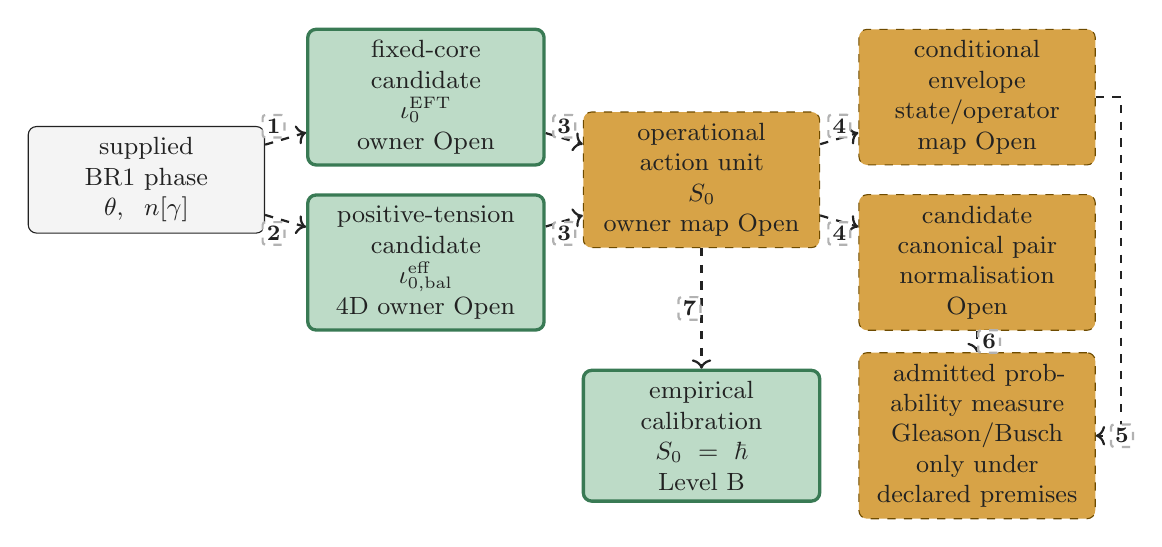
\begin{tikzpicture}[
  box/.style={draw, rounded corners=3pt, align=center, text width=2.72cm,
    minimum height=0.92cm, inner sep=4pt, font=\small},
  arrow/.style={->, thick, dashed, draw=ectInk},
  edgekey/.style={fill=white, draw=ectInk!35, rounded corners=1pt,
    inner sep=1.5pt, font=\footnotesize\bfseries, text=ectInk}
]
\node[box,ectExternal] (phase) at (0,0)
  {supplied BR1 phase\\$\theta,\;n[\gamma]$};
\node[box,ectConditional] (fixed) at (3.55,1.05)
  {fixed-core candidate\\$\iota_0^{\rm EFT}$\\owner Open};
\node[box,ectConditional] (balanced) at (3.55,-1.05)
  {positive-tension candidate\\$\iota_{0,\rm bal}^{\rm eff}$\\4D owner Open};
\node[box,ectOpen] (operational) at (7.05,0)
  {operational action unit\\$S_0$\\owner map Open};
\node[box,ectOpen] (wave) at (10.55,1.05)
  {conditional envelope\\state/operator map Open};
\node[box,ectOpen] (ccr) at (10.55,-1.05)
  {candidate canonical pair\\normalisation Open};
\node[box,ectOpen] (born) at (10.55,-3.25)
  {admitted probability measure\\Gleason/Busch only under\\declared premises};
\node[box,ectConditional] (hbar) at (7.05,-3.25)
  {empirical calibration\\$S_0=\hbar$\\Level B};
\draw[arrow] (phase) -- node[edgekey,above left]{1} (fixed);
\draw[arrow] (phase) -- node[edgekey,below left]{2} (balanced);
\draw[arrow] (fixed) -- node[edgekey,above]{3} (operational);
\draw[arrow] (balanced) -- node[edgekey,below]{3} (operational);
\draw[arrow] (operational) -- node[edgekey,above]{4} (wave);
\draw[arrow] (operational) -- node[edgekey,below]{4} (ccr);
\draw[arrow] (ccr) -- node[edgekey,right]{6} (born);
\draw[arrow] (wave.east) -- ++(0.32,0)
  |- node[edgekey,pos=0.72,right]{5} (born.east);
\draw[arrow] (operational) -- node[edgekey,left]{7} (hbar);
\end{tikzpicture}
\par\vspace{0.35em}
\begin{minipage}{0.97\textwidth}
\footnotesize
\textbf{Arrow key:}
\textbf{1} fixed length/profile;
\textbf{2} positive tension;
\textbf{3} still-Open owner map;
\textbf{4} supplied action unit;
\textbf{5} measure/state required;
\textbf{6} does not derive probability;
\textbf{7} separate physical match.
\end{minipage}
\caption{Status-separated dependency map for the coherent-sector
quantisation programme.  The phase-only fixed-core coefficient
$\iota_0^{\rm EFT}$ and the optional positive-tension coefficient
$\iota_{0,\rm bal}^{\rm eff}$ are distinct reduced-model candidates.  Neither is
silently identified with the operational action-unit slot $S_0$ used by the
conditional wave and canonical closures; each owner map is Open.  The later
$S_0=\hbar$ identification is a second, explicit Level~B empirical
calibration.  The
fixed-length bound and the minimisation of the supplied positive-tension 1D
functional are exact only inside their declared models.  No arrow derives a
probability measure, an outcome, a four-dimensional loop owner, or Planck's
constant.  Numbered arrow keys replace the former sloped micro-labels without
changing the graph topology.  Colour is redundant with literal status text
and dashed borders.}
\label{fig:qs_quantization_chain}
\end{figure}

For the present loop-based calculation status and the open
first-principles derivation of the action scale~$S_0$, see
Appendix~\ref{app:Sloop_calc}.

% ==============================================================
\subsection{Conditional charge lattice in a supplied compact local $U(1)$ completion}
\label{sec:charge_quantization}
% ==============================================================

\textit{Status: Level~A mathematics for integer representations of an
already supplied compact local $U(1)$ bundle.  P3--P5 do not derive that
bundle, its physical electromagnetic identification, matter
representations, the elementary unit $e_0$, an unbroken photon, or the
observed charge lattice; these remain Open.  The commutator route is
Level~B/Open because its operator algebra and $S_0$ normalisation are not
derived.  The electroweak $\mathbb Z_2$ quotient is conditional Level~B.}
Connection: compact phase
sector~(\S\ref{sec:qs_phase_dynamics}),
conditional local $U(1)$ completion~(\S\ref{sec:u1_emergence}),
Dirac quantisation
condition~\eqref{eq:qs_dirac_quantization},
electroweak
structure~(\S\ref{sec:common_origin}).

\subsubsection*{Problem statement: conservation versus quantisation
versus the observed charge spectrum}

Inside a supplied local $U(1)$ completion, Noether's theorem implies
conservation of the corresponding model charge.
This, however, is not yet the same as charge quantisation.
Conservation states that a charge, once assigned, is preserved.
Quantisation asks why the allowed charges belong to a discrete
lattice rather than a continuum.
Three levels must be kept sharply distinct:
\begin{enumerate}[label=(\roman*)]
  \item \emph{charge conservation},
    $\partial_\mu J^\mu = 0$, which is
    conditional on a supplied local symmetry and current
    (\S\ref{sec:u1_emergence});
  \item \emph{Abelian charge quantisation},
    $q \in \mathbb{Z}\cdot e_0$,
    i.e.\ why charges form a discrete lattice;
  \item \emph{the full observed Standard-Model charge pattern},
    $Q_{\rm em}/e=T_3+Y$ in the small-$Y$ convention, with values
    $0,\;\pm 1/3,\;\pm 2/3,\;\pm1$,
    which requires in addition electroweak embedding, the integer
    character $q_f=6Y_f$, the colour--weak centre interlock, and a
    derivation of the fermion representation content.
\end{enumerate}
The present subsection gives the conditional compact-group
representation theorem behind~(ii).  It does not establish that the ECT
compact phase is the physical electromagnetic bundle or that its
representation labels are observed electric charges; both~(ii) and~(iii)
remain Open as ECT identifications.

\subsubsection*{Conditional compact-phase route to an integer lattice}

For a supplied compact $U(1)$, fixed generator normalisation and
strongly continuous single-valued one-dimensional unitary characters, the
representation labels are integers.  The topology of a noncompact
$\mathbb R$ gauge group does not enforce such a lattice, although a
particular noncompact theory may still have a discrete matter spectrum from
separate dynamics or representation content.  Compactness fixes the
character labels under the stated premises; it fixes neither the elementary
unit $e_0$ nor the observed electric-charge map.  Which bundle and matter
content nature realises is an empirical input.

In ECT the supplied BR1 phase is compact,
$\theta\sim\theta+2\pi$~(\S\ref{sec:u1_emergence}).  This gives a
compact global variable.  It does not by itself derive a local gauge group,
its matter representations, or the physical electromagnetic charge
operator.  If those completion data identify the local fibre with compact
$U(1)$, the standard integer representation theorem below applies.

\begin{theorem}[Compact-$U(1)$ charge lattice]
\label{thm:charge_lattice}
Let the condensate phase sector be compact,
$\theta\sim\theta+2\pi$, and \emph{suppose} a supplied Abelian gauge
completion makes local rephasings the redundancy of this compact phase.
Then any matter excitation transforming in a strongly continuous,
single-valued one-dimensional unitary representation of this compact $U(1)$
has an integer character label and, after a separately supplied generator
normalisation $e_0$, carries charge
\begin{equation}
  \label{eq:charge_lattice_thm}
  q_n = n\,e_0, \qquad n\in\mathbb{Z},
\end{equation}
where $e_0$ is the elementary Abelian charge unit of the
condensate sector.
\end{theorem}

\paragraph{Proof.}
A charged excitation transforms as
$\psi\to e^{i\lambda\alpha(x)}\psi$
under a local gauge transformation with parameter~$\alpha$.
Because the gauge parameter is angular ($\alpha\sim\alpha+2\pi$),
the transformation with $\alpha=2\pi$ is the identity element of
compact $U(1)$.
Physical single-valuedness therefore requires
$e^{i2\pi\lambda}=1$, hence $\lambda\in\mathbb{Z}$.
Restoring the elementary charge unit~$e_0$, the covariant
derivative takes the form
$D_\mu = \partial_\mu - in\,e_0\,A_\mu$,
and the allowed charges are precisely
$q_n=n\,e_0$.
\hfill$\square$

\paragraph{Status.}
Theorem~\ref{thm:charge_lattice} is Level~A mathematics conditional on a
supplied compact local bundle, fixed generator normalisation and
strongly continuous single-valued one-dimensional unitary representation.
P5 does not derive those physical premises.  The mapping of the integer
label to electric charge, the elementary unit $e_0$, fractional Standard
Model charges, matter representations and anomaly constraints remain Open.
The theorem does \emph{not} require the canonical commutator
candidate~\eqref{eq:qs_commutator_candidate}.

\subsubsection*{Canonical generator spectrum (independent conditional route)}

A second route concerns the generator conjugate to the compact global-shift
orbit; it does not by itself reproduce the electric-charge lattice of
Theorem~\ref{thm:charge_lattice}.  This route first assumes that the
constant-shift orbit survives the physical gauge quotient/Gauss constraints
and has a finite nondegenerate symplectic form and finite nonzero inertia.
A constrained gauge zero mode such as
$L=I(\dot\theta-A_0)^2/2$ can instead impose $Q=0$ and remove the rotor.  In a
local chart with orbit coordinate $\alpha$ the formal signs are
$[\hat\alpha,\hat Q_\theta^{\rm phys}]=iS_0$ and
$[\hat Q_\theta^{\rm phys},\hat\alpha]=-iS_0$, while globally the unitary
$U_0=e^{i\alpha}$ obeys
$[\hat Q_\theta^{\rm phys},U_0]=S_0U_0$.
The reduced-generator relation
$\hat Q_\theta^{\rm red}=\hat Q_\theta^{\rm phys}/\Sigma_\theta$ additionally
assumes the exact constant action scaling and absence of an independently
normalised total-derivative/topological symplectic term.  A term
$a\dot\theta$ shifts the physical generator and flat holonomy; it may be
absorbed once into the twist below only after the action/domain convention is
fixed.  On sections of the supplied flat line bundle over
$L^2(S^1,d\alpha/2\pi)$, take the self-adjoint domain
$\psi(\alpha+2\pi)=e^{i\nu_{\rm tw}}\psi(\alpha)$,
Eq.~\eqref{eq:qs_dirac_quantization} gives
\[
 \operatorname{spec}\hat Q_\theta^{\rm phys}
 =S_0\left(\mathbb Z+\frac{\nu_{\rm tw}}{2\pi}\right).
\]
The reduced spectrum is
$(S_0/\Sigma_\theta)
(\mathbb Z+\nu_{\rm tw}/2\pi)$; only the separately supplied periodic domain
$\nu_{\rm tw}=0$ yields the unshifted lattices.  The surviving physical shift
orbit, Weyl representation and self-adjoint extension make the spectrum
discrete, but compactness alone selects neither the twist, $S_0$,
$\Sigma_\theta$ nor the physical charge map.  Level spacings identify
$S_0$ or $S_0/\Sigma_\theta$ only after the physical or reduced generator is
known; they do not determine the twist offset or $\Sigma_\theta$ by
themselves.

This route is Level~A operator mathematics under those premises and B/Open as
an ECT physical identification.  The compact-$U(1)$ representation theorem is
logically independent: its integer character lattice uses the group,
representation and elementary charge unit.  Identifying the canonical rotor
generator with observed electric charge requires an additional
representation/unit map and cannot be inferred from compactness alone.

\subsubsection*{Loop/holonomy viewpoint}

The same conclusion may be restated in the loop language natural
to ECT\@.
Transport of a charged excitation around a closed loop must return
the same physical state up to an allowed $U(1)$ phase.
Compatibility with the compact phase fibre forces the charge to lie
on the discrete lattice $q/e_0\in\mathbb{Z}$.

\subsubsection*{Electroweak conditional refinement}

If a completion explicitly supplies
$U(2)=[SU(2)\times U(1)_n]/\mathbb Z_2$, the $U(1)_n$ character must
be an integer.  With the full colour-compatible normalisation
$n=q_f=6Y_f$, a representation descends exactly when
$d_f+q_f\equiv0\pmod2$~\eqref{eq:charge_lattice}.  The quark doublet
$(d,q)=(1,1)$ therefore is a valid standalone $U(2)$ representation.
What standalone $U(2)$ lacks is the independent colour-$\mathbb Z_3$
triality interlock.  For colour singlets only one may alternatively use
$n_{\rm sing}=q_f/3=2Y_f$, which gives
$Q_{\rm em}/e=T_3+n_{\rm sing}/2=T_3+Y$; this weight is not integral
for quarks and must not be applied to them.

An even order-parameter potential establishes only
$V(\Phi)=V(-\Phi)$ for that potential.  It does not prove that the central
element acts trivially on every physical field, operator and line operator,
so it does not derive the physical $U(2)$ quotient.  The refinement is
Level~A conditional group mathematics and Open as an ECT identification.

\subsubsection*{Anomaly cancellation as a self-consistency
requirement}

For any supplied chiral gauge completion, anomaly cancellation is not an
external aesthetic criterion but a non-negotiable self-consistency
requirement: if
the chosen completion contains a chiral gauge sector, its supplied matter
content \emph{must} be anomaly-free; otherwise that completion is
inconsistent.  This does not derive the observed fermion representations or
show that they emerge from the condensate.  It constrains any acceptable
completion to satisfy the standard anomaly-cancellation conditions.
A systematic anomaly audit for a supplied chiral gauge completion,
including the standard electroweak consistency constraints, the
anomaly-transparency of the director coupling~$\mathcal{L}_5$, and
the open status of the colour-sector completion, is developed
in~\S\ref{sec:anomaly_architecture}.

\subsubsection*{Neutrino compatibility}

Within the full-weight standalone-$U(2)$ condition
$d_f+q_f\equiv0\pmod2$, a singlet with
$T=0$, $Y=0$ and hence $(d,q)=(0,0)$ has
$Q_{\rm em}=0$.  This is compatible with a sterile-neutrino-like state and
the supplied seesaw route, but it is not an independent derivation of that
state or its charge.

\subsubsection*{What remains open}

The compact-$U(1)$ result does not yet derive the full observed
Standard-Model electric-charge spectrum.
In particular:
\begin{enumerate}[label=(\roman*)]
  \item the appearance of quark charges $\pm e/3$ and $\pm 2e/3$
    requires the colour sector~(OP-GUT1) and the electroweak
    representation content~(OP-GUT3b);
  \item the precise equality $|Q_e|=|Q_p|$ requires
    anomaly-consistent representations~(OP-GUT6);
  \item the full observed charge pattern likely depends on the
    global structure of the complete low-energy gauge group,
    potentially of
    $(SU(3)\times SU(2)\times U(1)_Y)/\Gamma$ type with
    $\Gamma=\mathbb{Z}_6$, $\mathbb{Z}_3$, or
    $\mathbb{Z}_2$~\cite{AharonyEtAl2013};
  \item three fermion generations remain an open
    problem~(OP-GUT5).
\end{enumerate}

\subsubsection*{Comparison with other routes to charge quantisation}

\renewcommand{\arraystretch}{1.25}
\begin{longtable}{@{}L{2.7cm}L{4.0cm}L{4.0cm}L{4.0cm}@{}}
\caption{Comparison of routes to charge quantisation.}
\label{tab:charge_quant_comparison}\\
\toprule
Aspect & Standard QED & GUT embedding & ECT \\
\midrule
\endfirsthead
\toprule
Aspect & Standard QED & GUT embedding & ECT \\
\midrule
\endhead
\bottomrule
\endfoot
Why quantised
  & Not explained ($U(1)$ can be noncompact)
  & Group embedding forces it
  & Integer representations only after a compact local bundle is supplied \\
Status of derivation
  & Empirical input
  & GUT hypothesis required
  & Conditional mathematics A; ECT physical owner Open \\
Fractional charges
  & Empirical
  & Predicted by rep content
  & Requires EW$+$colour completion \\
Anomaly role
  & Empirical consistency check
  & Automatic within GUT
  & Mandatory consistency test of any supplied chiral completion \\
\bottomrule
\end{longtable}

\paragraph{Discriminant: ECT charge quantisation versus standard
approaches.}
The BR1 phase supplies a compact global variable, but a local compact
$U(1)$ bundle does not follow from that fact alone.  If a completion supplies
the bundle and its matter representations, integer representation labels
follow by standard group theory.  The local bundle, unbroken photon,
physical charge operator, elementary unit $e_0$, representation map and
observed spectrum remain part of the open gauge-matching programme
(OP-GUT4).

\paragraph{Falsifier for the charge-quantisation programme.}
The programme would be falsified if
(i)~the condensate phase sector were shown to be topologically
noncompact (contradicting the construction);
(ii)~a completed ECT gauge/matter sector produced anomaly-violating
representations;
or (iii)~the electroweak/colour completion failed to reproduce the
observed charge assignments.

\statussummary
\textit{Established~(Level~A mathematics, conditional premises):}
(i)~integer one-dimensional representations and
$q\in\mathbb Z\cdot e_0$ once a compact local $U(1)$ bundle, matter
representation and charge unit are supplied
(Theorem~\ref{thm:charge_lattice});


\textit{Architectural / consistency requirement:}
(i)~anomaly cancellation as a mandatory self-consistency
condition on any emergent chiral sector (consistency target,
not yet a derived representation theorem).

\textit{Conditional / Open:}
(i)~the conditional canonical-generator spectrum
of Eq.~\eqref{eq:qs_dirac_quantization}, after a physical Weyl
representation and self-adjoint domain are supplied; the periodic
$S_0\mathbb Z$ special case additionally requires $\nu_{\rm tw}=0$;
(ii)~standard $U(2)$ descent condition
$d_f+q_f\equiv0\pmod2$ after an integer character and quotient are supplied.
The physical quotient and charge map remain Open.

\textit{Open:}
(i)~the local compact bundle, unbroken photon, physical charge operator,
elementary unit and matter representation map;
(ii)~full observed electric-charge spectrum and hypercharge quantisation;
(iii)~full global gauge-group structure
$(SU(3)\times SU(2)\times U(1)_Y)/\Gamma$;
(iv)~observed fermion representation content.

\FloatBarrier
% ============================================================
\subsection{Uncertainty principle in the coherent branch}
\label{sec:qs_uncertainty}
% backward-compatibility alias:
\label{sec:uncertainty}
% ============================================================

\textit{Status: Level~A for the mathematical uncertainty inequality
once the canonical commutator structure of the smooth coherent branch
is admitted; Level~B for the physical normalisation of that inequality
by the observed $\hbar$, which depends on
Eq.~\eqref{eq:qs_S0_identification}.}

\medskip
The uncertainty relation discussed below inherits its status
directly from the canonical-bridge programme of
Section~\ref{sec:qs_ccr}: it is mathematically strict once the
commutator bridge is granted, but physically matched only after the
$S_0=\hbar$ identification.

The uncertainty principle is not introduced in ECT as an independent
axiom.
If the coherent branch already admits (i)~a wave-dynamical
representation, (ii)~a canonical organisation, and (iii)~a commutator
candidate normalised by the supplied coefficient $S_0$
(Section~\ref{sec:qs_ccr}), then the uncertainty relation follows as a
standard mathematical consequence.  This conditional theorem does not own
the coefficient or its physical matching.

\subsubsection*{Operator input}

The Robertson--Schr\"odinger theorem applies to supplied self-adjoint
operators on the common product domains required below.  For a noncompact
physical canonical pair $(q,p_{\rm phys})$, the conditional ECT bridge is
\begin{equation}
  \label{eq:qs_unc_comm}
  [\hat q,\hat p_{\rm phys}]=iS_0.
\end{equation}
After the separate empirical calibration
$S_0=\hbar$~\eqref{eq:qs_S0_identification}, this becomes
\begin{equation}
  \label{eq:qs_unc_comm_hbar}
  [\hat q,\hat p_{\rm phys}]=i\hbar .
\end{equation}
The representation, domains and physical owner are B/Open; the theorem
below is Level~A mathematics once they are supplied.

\subsubsection*{Robertson--Schr\"odinger inequality}

For self-adjoint $\hat A,\hat B$ and a normalised state in the domains of
$\hat A\hat B$ and $\hat B\hat A$, define
$\delta\hat A=\hat A-\langle\hat A\rangle$ and
$\delta\hat B=\hat B-\langle\hat B\rangle$.  Cauchy--Schwarz gives
\begin{equation}
  \label{eq:qs_robertson_schrodinger}
  (\Delta A)^2(\Delta B)^2
  \ge
  \frac14\bigl|\langle[\hat A,\hat B]\rangle\bigr|^2
  +\frac14\bigl|\langle\{\delta\hat A,\delta\hat B\}\rangle\bigr|^2 .
\end{equation}
Dropping the nonnegative covariance term gives
\begin{equation}
  \label{eq:qs_robertson}
  \Delta A\,\Delta B
  \ge \tfrac12\bigl|\langle[\hat A,\hat B]\rangle\bigr|.
\end{equation}
For the supplied physical pair,
\begin{equation}
  \label{eq:qs_uncertainty_S0}
  \Delta q\,\Delta p_{\rm phys}\ge\frac{S_0}{2},
\end{equation}
and, after $S_0=\hbar$,
\begin{equation}
  \label{eq:qs_uncertainty_hbar}
  \Delta q\,\Delta p_{\rm phys}\ge\frac{\hbar}{2}.
\end{equation}
If the reduced phase momentum is used on the corresponding local common
core, $\pi_\theta^{\rm phys}=\Sigma_\theta\pi_\theta^{\rm red}$ instead gives
$\Delta\theta\,\Delta\pi_\theta^{\rm red}
\ge S_0/(2\Sigma_\theta)$.  This local-chart statement does not create a
global self-adjoint angle operator.

\paragraph{Compact phase: use the unitary relation, not a naive angle bound.}
Multiplication by a sawtooth representative of the global orbit coordinate
$\alpha$ does not preserve the quasiperiodic self-adjoint domain of
$Q_\theta^{\rm phys}=-iS_0\partial_\alpha$.  Therefore
$\Delta\alpha\,\Delta Q_\theta^{\rm phys}\ge S_0/2$ is not a theorem:
indeed a rotor eigenstate has $\Delta Q_\theta^{\rm phys}=0$ while the
sawtooth angle has finite variance.  The missing hypothesis is precisely a
common invariant product domain.

The globally defined unitary $U_0=e^{i\alpha}$ obeys
$[Q_\theta^{\rm phys},U_0]=S_0U_0$.  Under the corresponding domain
assumptions, Cauchy--Schwarz yields the valid circular relation
\begin{equation}
  \label{eq:qs_compact_unitary_uncertainty}
  \Delta Q_\theta^{\rm phys}
  \sqrt{1-|\langle U_0\rangle|^2}
  \ge \frac{S_0}{2}|\langle U_0\rangle|.
\end{equation}
For a generator eigenstate $\langle U_0\rangle=0$, so the bound is
consistent with $\Delta Q_\theta^{\rm phys}=0$.  The twist
$\nu_{\rm tw}$, periodic special case and spectrum are those of
Eq.~\eqref{eq:qs_dirac_quantization}.  Integer field winding remains a
separate topological statement and derives neither the self-adjoint domain
nor a common physical $S_0$.

\subsubsection*{Interpretation}

The Robertson--Schr\"odinger inequality is a standard theorem once a Hilbert
space, physical operators, domains and their commutator are supplied.  ECT
reproduces that mathematics conditionally; it has not yet derived the physical
operators, commutator normalisation or universal $S_0$ from P1--P6.

\paragraph{Numerical anchor.}
After the identification $S_0=\hbar$, the uncertainty bound takes its
standard value
$\hbar/2 \approx 5.27\times10^{-35}\,\mathrm{J\,s}$.
For an electron confined to a hydrogen-like atomic scale
$\Delta x\sim a_0\approx0.529\,$\AA, one obtains
\begin{equation}
  \Delta p_{\min}\sim \frac{\hbar}{2a_0}
  \approx 1.0\times10^{-24}\,\mathrm{kg\,m/s},
\end{equation}
which is of the standard atomic order of magnitude.
ECT adds no correction to this result at the current level of the
coherent-branch closure: once $S_0=\hbar$ is matched, the usual
Heisenberg scale is reproduced exactly.

\paragraph{Discriminant: conditional theorem versus physical ownership.}
In standard axiomatic quantum mechanics, the uncertainty principle is a
theorem of the already assumed Hilbert-space and operator framework.
In ECT the same theorem holds in every supplied representation satisfying its
hypotheses.  The proposed compact-phase/canonical route is a programme for the
missing representation and normalisation, not a derivation that traces
uncertainty to winding or to a loop-generated action scale.

\paragraph{Falsifier for the uncertainty programme.}
The uncertainty programme would fail if a completed physical
canonical pair required a normalisation incompatible with its wave-sector
$S_0$, or if no self-adjoint/Weyl representation with the declared domains
could realise the compact generator relation
\eqref{eq:qs_dirac_quantization}.  Integer winding alone is not such a
compatibility condition.
At the observational level, any reproducible violation of the bound
$\Delta q\,\Delta p \ge \hbar/2$ in the regime where the standard
canonical description is known to apply would directly challenge the
canonical reading of the coherent branch.
No such violation has ever been observed.

\statussummary
\textit{Conditional Level~A mathematics:}
given a Hilbert space, the required common product domains and the
supplied physical-pair commutator~\eqref{eq:qs_unc_comm},
Eq.~\eqref{eq:qs_robertson_schrodinger} is the Robertson--Schr\"odinger
theorem and Eq.~\eqref{eq:qs_uncertainty_S0} its noncompact physical-pair
corollary.  The compact angle instead uses the unitary relation
\eqref{eq:qs_compact_unitary_uncertainty}.
Compact phase independently supplies an integer winding representation; it
does not prove that its global generator uses the same $S_0$ normalisation.
\textit{Level~B/Open:}
the physical commutator and Heisenberg form
$\Delta q\,\Delta p\ge\hbar/2$ require those owners and the separate matching
$S_0=\hbar$~\eqref{eq:qs_S0_identification}.
No experimental violation of this bound has been observed.

\paragraph{Bridge to the next chapter.}
With the Hilbert-space bridge, unitarity status, canonical
organisation, and uncertainty structure in place, the coherent branch
is ready for the next layer of analysis:
Euclidean path-dependence, exchange sectors, and the route to Dirac
structure.
Those questions are the subject of the next chapter.

% ============================================================

% ==============================================================
\section{Euclidean Path-Dependence, Quantum Nonclassicality, Statistics, and Dirac Structure}
\label{sec:qs_nonclassical}
% ==============================================================

\textit{Inputs: coherent-branch wave kinematics
(Section~\ref{sec:qs_wave_kinematics}), the Hilbert-space bridge
(Section~\ref{sec:qs_hilbert_bridge}), canonical structure
(Section~\ref{sec:qs_ccr}), and compact-phase topology~(BR1).
Aim: to separate three conditional structures of the coherent-sector
programme: Euclidean path-dependence in a supplied boundary-value problem;
exchange topology in a separately supplied defect-free point-configuration
space; and a possible Dirac sector after a physical Lorentzian metric,
spinor bundle and irreducible Clifford-factorisation action are supplied.
These are parallel inputs and results, not the implication chain
$O(4)\to O(3)\Rightarrow\mathbb Z_2\Rightarrow\mathrm{Spin}(3)
\Rightarrow\mathfrak{so}(1,3)\Rightarrow\mathrm{Clifford}\Rightarrow
\mathrm{Dirac}$.
Status: Level~A conditional mathematics for the elliptic two-sided
propagator in its declared BVP; Level~A topology for
$\pi_1(\mathcal M_2)=\mathbb Z_2$ in the declared defect-free
$\mathbb R^3$ point model, without representation selection; and Level~A
standard representation theory only after the physical metric/tetrad,
real form, spin structure and Clifford module have been supplied.
Interference, tunnelling and Dirac dynamics are Level~B conditional on their
additional actions, states and observable maps.  The physical spinorial
spectrum, CAR/OS completion, indefinite-causal-order reconstruction and the
interacting spin--statistics theorem remain Open.}

\subsection{Euclidean path-dependence: intermediate
results from both past and future}
\label{sec:path_dependence}

A fundamental feature of the ECT framework is that the Euclidean
equation of motion
\begin{equation}
  \left(-\nabla^2_E + m^2\right)\Phi(X) = 0,
  \qquad \nabla^2_E = \delta^{AB}\partial_A\partial_B,
\end{equation}
is an \emph{elliptic} partial differential equation.  Consequently,
the value of $\Phi$ at an interior point $X_m$ depends simultaneously
on boundary conditions at \emph{both} $w < w_m$ (the ``past'') and
$w > w_m$ (the ``future'').  The Euclidean Green's function
$G_E(X,X')$ is fully symmetric under $w\leftrightarrow -w$, encoding
this two-sided dependence.

\textbf{Exact boundary-value fact and Open quantum bridge.}
Two-sided Euclidean boundary dependence is also present in classical
elliptic systems, including electrostatics, and therefore supplies no
nonclassical consequence by itself.  The following items separate that exact
PDE fact from the additional quantum owners.

\begin{enumerate}

\item \textit{Quantum interference.}
  The four-dimensional Euclidean resolvent does \emph{not} obey the
  transition-kernel composition law printed here previously.  For
  $G_m=(-\nabla_E^2+m^2)^{-1}$ its exact spacetime convolution is
  \begin{equation}
    \int d^4X_m\,G_m(X_f,X_m)G_m(X_m,X_i)
    =-\frac{\partial}{\partial m^2}G_m(X_f,X_i),
    \label{eq:euclidean_resolvent_convolution}
  \end{equation}
  as follows immediately in momentum space.  A genuine composition law
  instead belongs to a time-sliced heat/transition kernel,
  $K_{T_1+T_2}(x_f,x_i)=\int d^3x_m\,
  K_{T_2}(x_f,x_m)K_{T_1}(x_m,x_i)$, after a slicing, state space and
  measure have been supplied.  Formal Euclidean--Lorentzian continuation
  can then connect the quadratic kernel to standard amplitude language;
  ellipticity alone does not derive the quantum measure or superposition
  rule.

\item \textit{Quantum tunnelling.}
  A supplied Euclidean quantum source model assigns a dimensionless weight
  $e^{-\mathcal I_E^\mu}$ to its integration configurations.  A tunnelling
  rate follows only after a named saddle or thimble, boundary conditions,
  determinant/prefactor and Euclidean--Lorentzian observable map are supplied.
  The bare P3 measure would use
  $\mathcal I_E^\mu=\kappa_{\rm P3}\mathcal I_E^{\rm P3}$; merely integrating
  over configurations does not derive an ECT tunnelling amplitude or identify
  its denominator with $S_0$.

\item \textit{Directionality and irreversibility.}
  The two-sided $w$-dependence of the Euclidean propagator does
  \emph{not} by itself produce an arrow of time: the Euclidean
  Green's function is symmetric under $w\leftrightarrow -w$ and
  treats past and future equally.  Coarse-graining may yield dissipative reduced dynamics, but it
  does not by itself define a forward/reverse probability ratio.  Such a
  ratio requires declared protocols, path measures, a time-reversal map, and
  local detailed balance.  Deriving those ECT objects remains OP-Q17.

\end{enumerate}

\paragraph{Structural significance.}
Two-sided Euclidean dependence is an exact property of the supplied elliptic
boundary-value problem.  It is neither sufficient nor discriminating for
interference, tunnelling, complex amplitudes, Born probabilities or
superposition as a quantum-state principle.  A physical bridge would
additionally require an admitted measure, complex/coherent structure, OS
reconstruction, composition law, preparation/state and observable map.  The
present text therefore retains ellipticity as Level-A mathematics in the
supplied model and the quantum interpretation as Open, not as an
architectural explanation.

\paragraph{What this does \emph{not} mean.}
The two-sided dependence along the Euclidean coordinate $w$ must not be
misread as controllable signalling from the future in Lorentzian time.
At the fundamental Euclidean level, $w$ is not yet the observed time
coordinate.
Only after a supplied scalar operator with $\beta(\beta-\alpha)<0$
(or $\alpha>\beta>0$ on the retained $\beta>0$ component), orientation and
initial-boundary prescription is there a conditional scalar notion of
retarded propagation.  A physical clock, cross-sector cone and operational
no-signalling theorem remain completion gates.  Thus ECT does not claim that
laboratory agents can influence the past; Euclidean two-sided boundary data
alone have no operational signalling interpretation.
This clarification also applies to indefinite-causal-order protocols:
ECT reads them as coherent manifestations of a pre-Lorentzian
two-sided amplitude structure, not as operational permission to signal
to the past.


\paragraph{Boundary-value compatibility only.}
Two-sided dependence in an elliptic Euclidean boundary-value problem does
not derive physical reverse $O(3)\!\to\!O(4)$ segments, their action weight,
or a laboratory quantum--classical threshold.  Establishing such segments
would require a saddle and backreaction calculation with declared boundary
conditions.  No causal-order, signalling, threshold-suppression, or
metric-signature consequence follows from ordinary two-sided boundary
dependence.  The retained claim is only that the Euclidean-first
boundary-value architecture is compatible with coherent amplitudes whose
Lorentzian reconstruction can depend on data specified on more than one
Euclidean boundary component.

\paragraph{Open comparison: Euclidean-first and Lorentzian formulations.}
The primary ECT arena is Euclidean and its supplied scalar equation is
elliptic, so two-sided boundary dependence precedes any proposed Lorentzian
reconstruction.  This ordering is an interpretive choice, not a derivation
of nonclassical amplitude structure: classical elliptic countermodels have
the same boundary dependence without quantum states or probabilities.  No
ECT-specific discriminator exists until the missing quantum bridge is
derived.

\paragraph{Falsifier for the path-dependence programme.}
The path-dependence programme would fail if the Euclidean two-sided
propagation structure, in the ordered Lorentzian
branch, proved structurally incompatible with the observed
interference, tunnelling, or superposition phenomena.
It would also be weakened if the elliptic Euclidean boundary-value
character could not be made consistent with the retarded causal
structure established elsewhere for the ordered branch.  A quantitative
test additionally requires a frozen Euclidean exponent
$\mathcal I_E^\mu$, measure, analytic-continuation prescription and
observable map; failure would reject that supplied bridge, not an undefined
universal weight.  No such physical ECT bridge is presently complete, so no
data comparison is claimed here.

% ============================================================

\subsubsection*{Indefinite causal order: compatibility, not an ECT prediction}
\label{sec:indefinite_causal_order}

\textit{Status: Open as an ECT-specific result.  Quantum-switch and
process-matrix predictions belong to standard quantum-information theory; the
present Euclidean-first architecture is compatible with them but has not
derived their process operators, causal witnesses, or platform dependence
\cite{Chiribella2012,Oreshkov2012}.}

The Procopio--Walther experiment~\cite{Procopio2015} reports high
interferometric visibility for a photonic quantum switch.  In a separately
declared pure-dephasing proxy one may define
\begin{equation}
  \Phi_{\rm vis}:=-\ln V,
  \label{eq:indef_causal_criterion}
\end{equation}
which gives $\Phi_{\rm vis}=0.0060\pm0.0020$ from
$V=0.994\pm0.002$.  This is a transformation of a reported visibility, not a
microscopic condensate calculation and not evidence for reverse Euclidean
segments.  A universal order-resource threshold at $\Phi=1$ is not derived.


\subsubsection*{The Procopio--Walther quantum switch}

Procopio et al.~\cite{Procopio2015} realised coherent control of
the order of two operations.  ECT is compatible with that process but has not
derived its process operator, causal witness, or apparatus kernel; the result
is not evidence for physical reverse trajectories.

\subsubsection*{Programme-level expectations for indefinite-order
experiments}

Platform-level expectations require an ECT record operator and
noise kernel.  Without those owners, temperature, coupling, and visibility
trends are ordinary open-system hypotheses rather than ECT predictions.

\paragraph{Expectation 1 (coherence-threshold degradation).}

Loss of a switch advantage must be computed from the platform's
process matrix and declared record channel; no universal crossover follows
from one scalar proxy.

\paragraph{Expectation 2 (environmental scaling).}

Increasing a specified environmental coupling can reduce a
coherent-control witness, but the scaling depends on the coupled operator,
spectrum, state, and protocol.  An unresolved ``bath size'' alone is not a
predictive variable.

\paragraph{Expectation 3 (temperature sensitivity).}

Temperature sensitivity is conditional on a thermal state and
the platform spectral density.  No universal ECT temperature law is asserted
without a KMS state and the relevant coupling.
ECT becomes testable in this sector only after it supplies a platform record
operator and kernel that predicts a correction to the standard switch
statistics.  Until then the result is interpretive compatibility and provides
no ECT-specific discriminator.



\paragraph{Quantitative dephasing estimate.}

The reported visibility $V=0.994\pm0.002$ gives the source-model
proxy $\Phi_{\rm vis}:=-\ln V=0.0060\pm0.0020$.  This arithmetic is retained,
but it is neither a microscopic condensate calculation nor an ECT-specific
fit~\cite{Procopio2015}.
\subsubsection*{Delayed choice, quantum erasure, and entanglement swapping}


\subsubsection*{Interpretive conclusion}

Indefinite-order experiments are compatible with a pre-Lorentzian
two-sided amplitude architecture, while process-matrix theory already
describes them operationally~\cite{Oreshkov2012}.  ECT becomes discriminating
only after predicting a held-out correction.
Delayed-choice and quantum-eraser experiments are described consistently by
ordinary quantum amplitudes, conditioning, and later classical comparison;
they do not enable signalling to the past.  Delayed-choice entanglement
swapping likewise reorganises conditioned correlations without changing an
earlier locally available record
\cite{Wheeler1978,Wheeler1984,Jacques2007,ScullyDruhl1982,Kim2000,Ma2012}.
ECT presently reproduces no
platform-specific statistic beyond that standard description.

The Euclidean boundary-value picture may be used as an interpretation, but it
does not establish literal reverse $O(3)\to O(4)$ transitions, a universal
coherence threshold, or a new retrocausal mechanism.  Any ECT claim in this
family requires derived apparatus couplings and a held-out quantitative
deviation.  The current status is Open as an ECT discriminator.


\paragraph{Wheeler's delayed-choice experiment.}

Wheeler/Jacques delayed choice changes the late measurement basis
and hence conditioned statistics without signalling to the past
\cite{Wheeler1978,Wheeler1984,Jacques2007}.  ECT currently offers a
boundary-value interpretation, not an experiment-specific correction.

\paragraph{Comparison with standard quantum theory.}

Standard superposition and the Born rule quantitatively own the
delayed-choice outcome.  ECT's present addition is only the statement that
global Euclidean boundary data need not be organised by a primitive
one-sided time before Lorentzian reconstruction.

\paragraph{Quantum eraser.}

In a quantum eraser, which-path marking removes interference in
the unconditioned ensemble and coincidence conditioning restores it only in
selected subensembles~\cite{ScullyDruhl1982,Kim2000}.  No completed
macroscopic collapse is reversed.

\paragraph{Comparison with standard quantum theory.}

The density-matrix and conditional-probability account is the
quantitative owner of quantum erasure.  A medium interpretation may identify
the physical record degrees of freedom only after their coupling and trace
are explicitly derived.

\paragraph{Delayed-choice entanglement swapping.}

Delayed-choice entanglement swapping changes the correlation class
identified after Bell-state analysis and later classical comparison; no
earlier local record is changed~\cite{Ma2012}.

\paragraph{Comparison with standard quantum theory.}

Entangled projection and classical record comparison already
account for the observations.  The common-medium picture is at present an
interpretation and supplies no new numerical prediction.

\paragraph{Summary of delayed-choice experiments.}

All three families preserve operational no-signalling.  Global
Euclidean boundary-value dependence must not be described as controllable
retrocausation in any supplied Lorentzian observable completion.
\begin{longtable}{@{}L{4.0cm}L{6.0cm}L{4.4cm}@{}}
\toprule
Experiment family & Standard operational statement & ECT status \\
\midrule
\endfirsthead
\toprule
Experiment family & Standard operational statement & ECT status \\
\midrule
\endhead
\bottomrule
\endfoot
Wheeler/Jacques delayed choice & Late basis choice changes conditioned statistics without past signalling & Compatible; no ECT correction derived \\
Quantum eraser & Interference reappears only in conditioned subensembles after record erasure & Standard channel result; ECT Open \\
Delayed-choice entanglement swapping & Correlations are identified after Bell analysis and classical comparison & Standard result; ECT Open \\
Procopio quantum switch & High-visibility coherent control of operation order & $\Phi_{\rm vis}=-\ln V$ is a source proxy only \\
\end{longtable}


\paragraph{Requirements for a future programme-level discriminator.}

A genuine ECT discriminator would be a platform-specific,
pre-registered correction computed from the condensate coupling and record
kernel.  Generic visibility loss under added noise is not such a
discriminator.
\subsubsection*{Wigner's friend paradox}

\textit{Status: interpretive / Level~B.  ECT does not modify the
operational predictions but provides a structural reframing of the
problem.}

In the Wigner's friend scenario, an observer (the ``friend'')
performs a measurement inside a sealed laboratory, while a
superobserver (Wigner) treats the entire laboratory as a quantum
system.
In the standard presentation, the paradox is that the friend
assigns a definite outcome while Wigner assigns a superposition.

In the ECT reading, the tension is reformulated structurally rather
than eliminated by a new measurement postulate.
The friend's measurement device may form a robust reduced-state
record in a specified channel.  This does not derive one realised outcome;
the update rule remains OP-Q19.
Wigner, if treated as external to that record-generating process,
may still assign a more weakly reduced description to the laboratory as
a whole, but only insofar as the relevant lab--environment coarse
graining has not yet been specified at his level of description.
ECT therefore shifts the question from ``who is observing'' to
``which degrees of freedom have already been locked by
environmentally amplified record formation''.

\paragraph{Comparison with standard quantum theory.}
Standard quantum theory can accommodate both the
friend-collapsed and Wigner-superposed descriptions within the
relative-state formalism, but does not by itself privilege one physical
criterion for when a definite record should count as established.
ECT proposes such a criterion only at closure level:
large effective environmental locking of the record-generating degrees
of freedom.
This is a structural closure-level reading of the paradox, not yet a
completed model-independent theorem of measurement.


\subsection{Two-sided Euclidean paths and protocol-defined reverse weights}
\label{sec:pes_reverse_path}

The Euclidean functional integral can contain both orientations of a path,
but this kinematic fact does not define thermodynamic forward and reverse
experiments.  For a declared protocol and measurable time-reversal
involution $\Theta$, transport the normalised reverse measure to the
forward path space as $Q=P_R^\Theta$, with $Q(A)=P_R(\Theta A)$.  Assuming
$P_F\ll Q$, define
\begin{equation}
  \Sigma[\gamma]
  :=\ln\!\left(\frac{dP_F}{dQ}(\gamma)\right),
  \qquad
  \frac{dQ}{dP_F}(\gamma)=e^{-\Sigma[\gamma]}
  \quad\hbox{when }P_F\sim Q .
  \label{eq:P_back_fwd}
\end{equation}
Thus one-way absolute continuity is enough to define $\Sigma$ $P_F$-almost
surely, whereas the reciprocal and the standard unit integral-fluctuation
identity require mutual absolute continuity.  Singular reverse weight
belongs to the separate absolute-irreversibility case.  This is a protocol
definition, not a universal identification of a reverse/forward path ratio
with the exponential of a dephasing scalar.  A pairwise dephasing exponent
measures loss of interference between alternatives; it is not a
path-probability ratio.  An ECT fluctuation relation remains Open pending
derived forward/reverse measures, initial ensembles and local detailed
balance.

\subsection{Tunnelling from a supplied Euclidean saddle}
\label{sec:pes_tunnelling}

\textit{Status: Level~A external mathematics for the standard leading WKB
exponent under its stated one-particle assumptions; Level~B for using a
specified Euclidean saddle in a supplied ECT functional with declared
physical-action and measure owners; Open for a
literal excursion through the fourth Euclidean coordinate or an ECT-specific
correction to a measured tunnelling rate.}

\subsubsection*{WKB exponent and Euclidean rederivation}

Let a one-dimensional Hamiltonian $H=p^2/(2m)+V(x)$ have simple turning
points $x_-<x_+$ at energy $E$, with $V(x)>E$ between them.  At leading WKB order the positive physical under-barrier action of
this supplied external one-particle source model is
\begin{equation}
  \label{eq:instanton_action}
  S_{\rm WKB}(E)
  :=\int_{x_-}^{x_+}dx\,\sqrt{2m\,[V(x)-E]},
  \qquad
  T_{\rm WKB}(E)\asymp e^{-2S_{\rm WKB}(E)/\hbar},
\end{equation}
up to the standard connection prefactor and higher semiclassical orders.
This formula follows without assigning ontological reality to an extra
coordinate.

The same exponent has a controlled Euclidean-saddle derivation.  For the energy-shifted physical Euclidean action of that external
source model
\[
 S_E[x]-E\Delta\tau_E
 =\int d\tau_E\,[\tfrac12m\dot x^2+V(x)-E],
\]
the zero-energy first integral of the shifted Euclidean problem is
$m\dot x^2/2=V-E$.  Evaluating the shifted action on one monotone crossing
therefore gives
\[
 S_E[x_{\rm sad}]-E\Delta\tau_E
 =\int_{x_-}^{x_+}dx\,\sqrt{2m[V(x)-E]}
 =S_{\rm WKB}(E).
\]
For false-vacuum or metastable decay, by contrast, the standard quantum
rate has the form $\Gamma\simeq A e^{-B/\hbar}$ with a vacuum-subtracted
\emph{bounce} action $B$ and a fluctuation/zero-mode prefactor $A$; that
bounce problem must not be identified with the one-crossing transmission
exponent without its own boundary conditions.  The $\hbar$ in these displayed
formulae belongs to the externally calibrated quantum problem.  A prospective ECT Euclidean channel must instead supply a
vacuum-subtracted physical bounce action $B_{\rm ch}^{\rm phys}$ and its own
finite positive path-integral denominator $\Sigma_{\rm PI,ch}$, giving
$\exp[-B_{\rm ch}^{\rm phys}/\Sigma_{\rm PI,ch}]$.  The undeformed P3
quartic has degenerate minima, $\epsilon=\Delta V=0$, and owns no finite
false-vacuum bounce by itself: its thin-wall $R$ and $B$ diverge.  Only an
explicitly biased/deformed P3 potential, finite boundary/protocol or another
named channel could supply a positive finite
$\Delta\mathcal I_E^{\rm P3}$ and the conditional factor
$\exp[-\kappa_{\rm P3}\Delta\mathcal I_E^{\rm P3}]$.  Complex thimbles
require their own contour interpretation.  No map from a channel denominator
to the canonical $S_0$ or external $\hbar$ is presently derived.

\subsubsection*{What a fourth-spatial bypass would require}

P1 states that the microscopic manifold is four-dimensional and Euclidean;
it does not specify the particle/worldline reduction or a barrier
$V(\mathbf x,w)$.  In particular, writing only $V(\mathbf x)$ normally means
that the potential is independent of $w$ and hence extends uniformly along
that coordinate.  It does \emph{not} imply an opening around the barrier.
Conversely, a barrier localised in $w$ would be a new operator and boundary
assumption.

If one properly normalised ECT action and boundary-value problem actually
supply a stationary four-coordinate
saddle $X^A_{\rm sad}(\sigma)$, its coordinate excursion may be defined by
\begin{equation}
  \label{eq:detour_length}
  \Delta w_{\rm sad}
  :=\max_\sigma w_{\rm sad}(\sigma)-\min_\sigma w_{\rm sad}(\sigma).
\end{equation}
This definition predicts neither $\Delta w_{\rm sad}\ne0$ nor
$\Delta w_{\rm sad}\sim x_+-x_-$.  The former estimate
$\mathcal I/p_w$ was only a dimensionally admissible ratio and cannot prove a
geometric path, because no $p_w$, $V(\mathbf x,w)$, variational saddle or
projection map owned it.

The preserved ECT route is therefore conditional: derive from one action
(i) the physical tunnelling coordinate and its canonical kinetic term,
(ii) the full $w$-dependent barrier/operator and boundary state,
(iii) the constrained Euclidean saddle and determinant, and
(iv) the analytic-continuation and detector map.  Only then may one compare
the saddle action with $S_{\rm WKB}(E)$ and ask whether a nonzero
$\Delta w_{\rm sad}$ changes the transmission exponent or prefactor.  The
gate is a preregistered barrier- and platform-specific deviation after the
ordinary multidimensional instanton calculation; generic agreement with WKB
is not an ECT discriminator.

\subsubsection*{Connection to PES-R and protocol reversal}

The tunnelling exponent is owned by the supplied saddle and boundary-value
problem.  PES-R can subsequently classify a metastable state's physical pole
width, finite-time survival and record formation for a declared channel; it
does not derive the saddle.  A coordinate derivative $\partial_w\Psi$, the
translation susceptibility $\Gamma_{\rm tr}$, a pairwise dephasing exponent
and a decay rate are distinct objects.

Echo/control protocols may refocus phases or erase a specified record, but
they neither implement a literal return to the bare $O(4)$ phase nor furnish
a universal reverse-path law.  Euclidean boundary correlations likewise do
not become controllable Lorentzian retrocausation.  Thus the standard
semiclassical exponent survives, while the literal fourth-spatial bypass and
any new numerical law remain Open behind the stated action/saddle/detector
gate.

\statussummary
\textit{Established~(Level~A):}
the Euclidean coherent-field equation is elliptic, so interior values
depend on boundary data from both sides of the Euclidean ordering
coordinate.
\textit{Level~B route / Open physical ECT:}
after an admitted quantum measure and coherent structure, or a named Euclidean
saddle, state, continuation and observable map are supplied, standard Euclidean
methods can organise interference or tunnelling.  Two-sided elliptic
dependence alone derives neither phenomenon, and no ECT-specific amplitude or
rate is presently obtained.  The quantitative reconstruction of operational
indefinite-causal-order protocols, switch correlators, and platform-dependent
degradation laws from condensate dynamics likewise remains incomplete.

% ============================================================
\subsection{Quantum statistics: exchange sectors and spinorial compatibility}
\label{sec:qs_statistics}
% ============================================================

\textit{Status: Level~A topology inside the declared defect-free
$\mathbb R^3$ point-excitation configuration space:
$\pi_1(\mathcal M_2)=\mathbb Z_2$, giving two homotopy classes.  Its
application to physical ECT is conditional on a separately supplied physical
three-dimensional slice and excitation map; P1 and P4 do not derive either.
The characters $\pm1$ follow only after restricting to one-dimensional
unitary representations.  Level~B is a route from those admitted characters
and separately supplied tensor/spinor sectors to the familiar exchange
assignments.  Open~(OP-Q11) are the physical slice and excitation map,
representation selection, the treatment of higher-dimensional $S_N$ sectors,
the spin--statistics theorem, CAR and the many-excitation reconstruction.
Connection: P4, P5, \S\ref{sec:fermion_statistics},
\S\ref{sec:qs_dirac}, and \S\ref{sec:qs_entanglement}.}

\medskip
Belonging to the same emergent mode sector is not by itself a proof that
physical excitations have no unresolved core, orientation, internal or
environmental labels.  If two physical ECT excitations are independently
shown to be identical unlabeled point excitations in defect-free
$\mathbb R^3$, their supplied coordinate configuration space is the quotient
by exchange used below.  ECT has not yet derived that excitation/identity map
or excluded additional discrete fibres and sectors.  The quotient-space
topology is therefore a conditional theorem for the declared point-excitation
model, not a derivation of physical indistinguishability.

If the quantum sector of ECT is to reproduce many-particle physics, it
must derive the physical spatial slice, relevant configuration space, state
representation and observed exchange assignment.  At present the declared
defect-free $\mathbb R^3$ point model supplies only a conditional
three-dimensional homotopy input.  ECT has not derived the physical
three-dimensional slice, point-excitation configuration space,
representation or physical assignment; these are separate completion steps.

\subsubsection*{Exchange topology}

For two identical excitations in the declared defect-free $\mathbb R^3$
point model, the reduced configuration space is
\begin{equation}
  \label{eq:qs_exchange_space}
  \mathcal{M}_2
  =
  \bigl(\mathbb{R}^3\times\mathbb{R}^3\setminus\Delta\bigr)/S_2,
\end{equation}
whose fundamental group is
\begin{equation}
  \label{eq:qs_exchange_pi1}
  \pi_1(\mathcal{M}_2) = \mathbb{Z}_2.
\end{equation}
This yields exactly two homotopy classes of loops~(Level~A topology for
the supplied configuration space).  Calling them symmetric and
antisymmetric already adds a representation: the one-dimensional unitary
characters of $\mathbb Z_2$ are $+1$ and $-1$.  The topology does not choose
one for a species or supply a quantum amplitude.

\paragraph{What the declared defect-free configuration-space model establishes.}
For identical point excitations in defect-free $\mathbb R^d$ with $d\ge3$
and the collision diagonal removed, exchange loops reduce to the
permutation-group topology; for two excitations this is $\mathbb Z_2$.
This statement is not extended to arbitrary multiply connected ambient
spaces, whose independent cycles can contribute additional loop classes.  In $d=2$, the braid
group is richer and supports continuous Abelian anyonic phases
\cite{Wilczek1982,Nayak2008}.  Conditional on P1 and on the point-excitation
configuration-space model, P4 therefore blocks importing such a generic
two-dimensional braid phase into the primary branch.  It does not derive
bosons, fermions, representation selection or physical statistics.

\paragraph{External QED reference.}
Observed particle physics in $3+1$ dimensions exhibits exactly the
bosonic/fermionic dichotomy for fundamental excitations: photons and
gauge bosons are bosonic, while electrons, neutrinos, and quarks are
fermionic.
By contrast, anyonic exchange has been observed only in effectively
two-dimensional condensed-matter systems, where braid topology differs
from the $3+1$-dimensional particle-exchange problem.
This empirical split is compatible with a future physical completion whose
spatial slices are three-dimensional, while anyonic
statistics remains an emergent lower-dimensional quasiparticle
phenomenon rather than a fundamental exchange law of the coherent
branch.

\subsubsection*{Representation-theoretic compatibility}

Given the $O(3)$ stabiliser of the supplied P4 vector, a separately supplied
excitation sector may be organised in its representations.  If a
one-dimensional exchange character is also selected, integer-spin/$+1$ and
half-integer-spin/$-1$ are compatible with the standard assignment.  This is
an admissible pairing, not a theorem derived from the two group facts.

\paragraph{Medium reading of exchange~(P5).}
P5 motivates treating same-species excitations as modes of one medium, but it
does not determine their configuration space, state representation or
exchange character.  Those owners must be derived in the completed
many-excitation sector; the full spin--statistics link remains Open.

\paragraph{Conditional canonical-normalisation no-go in a supplied
fermionic EFT.}
\label{par:smooth_pauli_exactness}
A natural question is whether a \emph{supplied} local fermionic/CAR
completion allows small violations of the Pauli principle in the
presence of a spatially varying ordered condensate, such as inside
strong gravitational fields or in dense astrophysical regimes. The answer
obtained in this conditional EFT is essentially the opposite of
what a naive gradient estimate might suggest: smooth local
inhomogeneity of the ordered condensate does not by itself
furnish a mechanism for violating fermionic exclusion on the
coherent ordered branch.

For a local first-order fermionic EFT with a smooth and strictly
positive temporal kinetic coefficient $\mathcal{K}(x)>0$ multiplying
$i\,\psi^\dagger\partial_t\psi$, a general condensate-dependent
temporal kinetic term of the form
$i\,\mathcal{K}(x)\,\psi^\dagger\partial_t\psi+\cdots$
can be brought to canonical form by the local field redefinition
\begin{equation}
  \chi_\alpha(x)\;\equiv\;\mathcal{K}(x)^{1/2}\,
    \psi_\alpha(x),
  \label{eq:psi_to_chi_normalisation}
\end{equation}
after which the equal-time anticommutator takes the standard
canonical form
\begin{equation}
  \{\chi_\alpha(t,\mathbf{x}),\chi_\beta^\dagger(t,\mathbf{y})\}
  = \delta_{\alpha\beta}\,\delta^{(3)}(\mathbf{x}-\mathbf{y}),
  \label{eq:chi_CAR}
\end{equation}
and local interaction terms (including condensate-dependent mass
$M(\phi,n)\bar\psi\psi$, the candidate preferred-direction operator
$\mu_5(\phi,n)\bar\psi\gamma^A n_A\psi$, and local
four-fermion operators $C_k(\phi,n)\mathcal{O}_k^{(4f)}$) modify
the dynamics of fermionic modes without altering the underlying
exclusion algebra. A full technical exposition of the canonical
normalisation procedure and its explicitly conditional scope is given in
Appendix~\ref{app:pauli_exactness}.

\textit{Restricted conditional statement.}
If the eventual fermionic reconstruction closes to a local first-order
Grassmann theory with a smooth positive scalar kinetic factor and standard
CAR before the rescaling, the rescaling above preserves the CAR.  This
excludes only a statistics violation generated solely by that scalar
normalisation.  Any departure would require failure of at least one supplied
premise.  Non-exhaustive possibilities include:
\begin{enumerate}[label=(\roman*)]
  \item a noncanonical kinetic or symplectic structure, a singular or
    sign-changing kinetic operator, or a failure of the assumed local CAR;
  \item \emph{nonlocal branch mixing} --- sector couplings that
    cannot be cast in the form of a local first-order fermionic
    EFT on the coherent branch.
  \item \emph{topological or defect sectors of the ordered
    condensate} beyond the ordinary coherent branch (e.g.\ 
    condensate-defect backgrounds with nontrivial $\pi_k$
    content; cf.\ the topological-sector catalogue in
    Section~\ref{sec:particle_structure}).
  \item \emph{branch-transition / coherence-loss regions}, where
    the ordered-branch description itself fails and the
    fermionic reconstruction programme ceases to close.
\end{enumerate}
This list is not a classification theorem.  Physical fermion
reconstruction, spin--statistics assumptions, the operator domain and any
nonstandard completion remain Open under OP-Q11 and OP-Q21.

\textit{Scope: no astrophysical inference.}
The equivalence principle removes a connection at a point but does not fix
the order or Wilson coefficients of curvature-dependent local operators.
The present local canonical-normalisation argument therefore implies no
packet-mismatch scaling, compact-object estimate or astrophysical exclusion
window.  White-dwarf and neutron-star matter cannot be classified here
without a physical ECT fermion action, CAR owner, curvature operators, state
and observable map.

\textit{Conditional on the fermionic reconstruction programme.}
At the present stage, the no-go statement is therefore conditional
not on the canonical-normalisation argument itself, which is
technically complete within the local first-order EFT closure
described above, but on the completion of the fermionic
reconstruction from the exchange-topological and
representation-theoretic sector
(\S\ref{sec:qs_statistics},~\S\ref{sec:qs_dirac}) to the full
operator-level canonical anticommutation
structure~(OP-Q11,~OP-Q21).

\subsubsection*{What is and is not claimed}

The exact topological input is the supplied configuration-space result
$\pi_1(\mathcal M_2)=\mathbb Z_2$ in the declared defect-free $\mathbb R^3$
point model.  It gives two
homotopy classes and, after an additional one-dimensional-unitary-sector
assumption, the characters $\pm1$.  It does not select either character,
construct CAR/Fock space, or identify spin with exchange.  For $N\ge3$, the
group $S_N$ also admits higher-dimensional representations, so excluding
parastatistical descriptions requires the standard additional locality and
relativistic quantum assumptions.

\paragraph{Connection to downstream programmes.}
This corrected input remains useful conditionally.  It supplies the
exchange-loop topology for the fermion, Dirac and entanglement programmes
inside the declared defect-free $\mathbb R^3$ point model and rules out a
generic two-dimensional braid phase only after a physical three-dimensional
slice and point-excitation map are supplied.  Each downstream programme must
still specify its physical slice, state space, representation, observable
algebra and local dynamics.

\paragraph{Discriminant and recovery route.}
In two spatial dimensions the braid group permits continuous Abelian anyonic
phases.  In three spatial dimensions the point-particle exchange group
collapses to the permutation group; for two particles it is $\mathbb Z_2$.
That dimensional contrast is Level-A topology for the separately supplied
defect-free $\mathbb R^3$ point-configuration model.  Its application to
physical ECT is conditional on the physical spatial slice and excitation
map, neither of which follows from P1/P4.  It is not an ECT-specific
prediction of bosons, fermions or the absence of every parastatistical
description.  A physical discriminant would require a completed excitation
sector and an exchange-interferometry observable specified before data.

\statussummary
\textit{Established~(Level~A, conditional on the separately supplied
defect-free $\mathbb R^3$ point-excitation configuration space):}
$\pi_1(\mathcal M_2)=\mathbb Z_2$, and continuous Abelian braid phases of the
two-dimensional anyon type are unavailable in that model.  P1 and P4 do not
by themselves derive the physical $\mathbb R^3$ slice, particle identity or
excitation map.

\textit{Level~B route:} after selecting a one-dimensional unitary
representation, the characters $+1$ and $-1$ are compatible with bosonic and
fermionic exchange sectors.

\textit{Open~(OP-Q11):} the physical excitation space, representation
selection, treatment or reduction of higher-dimensional $S_N$ sectors, the
spin--statistics theorem, CAR and the many-excitation reconstruction.

% ============================================================

\renewcommand{\arraystretch}{1.3}
\begin{longtable}{@{}L{3.2cm}L{5.0cm}L{6.3cm}@{}}
\caption{Quantum statistics in ECT vs standard frameworks.}\label{tab:statistics_comparison}\\
\toprule
Aspect & Standard QM/QFT & ECT \\
\midrule
\endfirsthead
\toprule
Aspect & Standard QM/QFT & ECT \\
\midrule
\endhead
\bottomrule
\endfoot
Route to bosonic/fermionic split
& Full spin-statistics theorem within an already assumed operator framework
& Topological exchange dichotomy in $d=3$ plus structural compatibility with ordered-branch representation content (Level~B; not yet full PLZ; free-kernel Euclidean OS test Level~A, Q11.1a) \\
Operator-algebra basis
& Bosonic/fermionic operator algebra fixed within the standard quantised-field framework
& Topological and representation-theoretic skeleton established; full operator-algebraic completion remains open \\
Pauli exclusion
& Follows for fermions once the fermionic operator algebra / spin-statistics structure is imposed
& Structural Level~B consequence once the spinorial sector and spin-statistics route are combined; not yet a full operator-level theorem \\
Full PLZ theorem
& Yes
& Open \\
Beyond present closure
& Standard many-body framework available
& Full many-body fermionic construction remains open \\
\bottomrule
\end{longtable}

\subsection{Representation-theoretic route to Dirac structure}
\label{sec:qs_dirac}
% ============================================================

\textit{Status: the supplied $O(4)\to O(3)$ director branch, the
exchange quotient of identical points in defect-free $\mathbb R^3$, the
double cover of a supplied connected rotation/Lorentz group, and the
irreducible Clifford factorisation are distinct conditional constructions.
Each standard mathematical statement is Level~A under its own hypotheses;
no one of them derives the next.  Dirac-type dynamics is Level~B conditional
only after a physical Lorentzian metric/tetrad, spin structure, realised
four-component irreducible Clifford module and action are supplied.
The physical spinorial spectrum, masses, gauge couplings, CAR/Fock/OS
completion and interacting spin--statistics theorem remain Open.
Connection: exchange topology (\S\ref{sec:qs_statistics}), the scoped
Clifford theorem (Eq.~\eqref{eq:scoped_clifford_factorisation}), fermionic
programme (\S\ref{sec:fermion_statistics}), Open electroweak/chirality
programme (\S\ref{sec:ew_embedding}), fifth-force coupling
(\S\ref{sec:fifth_coupling}), and entanglement
(\S\ref{sec:qs_entanglement}).}

\medskip
The exchange-sector analysis of Section~\ref{sec:qs_statistics}
establishes two loop classes and two one-dimensional character choices in
the declared configuration-space model.  It does not select a species
assignment and does not establish that the ECT broken phase physically
contains either bosonic or fermionic particles.
The present subsection shows that the symmetry structure of the broken
condensate provides a natural representation-theoretic route to
the Dirac structure.

\paragraph{Full structural chain from the ordered branch to Dirac
form.}
The representation-theoretic route to Dirac structure should be read as
the final part of a longer ordered-branch chain:
\begin{enumerate}[label=(\roman*)]
  \item P4 supplies a nonzero vector with $O(3)$ stabiliser; a physical
  transition, branch and three-space interpretation remain Open;
  \item after a physical three-dimensional spatial slice is separately
  supplied, the exchange topology of
  identical excitations is $\pi_1(\mathcal{M}_2)=\mathbb{Z}_2$
  (Section~\ref{sec:qs_statistics});
  \item the residual rotational sector admits the spinorial double cover
  $\mathrm{Spin}(3)\to SO(3)$;
  \item after a physical metric/clock and the standard complex generator
  continuation are supplied, the usual Lorentz algebra
  $\mathfrak{so}(1,3)$ is available conditionally;
  \item a supplied spinor representation of that algebra carries the standard
  Clifford structure~\eqref{eq:qs_clifford};
  \item within a supplied minimal local linear first-order Lorentz-covariant
  fermion closure, the corresponding free dynamics is Dirac-type.
\end{enumerate}
The exchange topology and Euclidean group facts are structural results.  The
physical Lorentz metric, fermion representation, Clifford action and Dirac
dynamics are conditional completion data, not consequences of P4 alone.

\subsubsection*{Conditional continuation from $O(4)$ generators to the
Lorentz algebra}

The Lie algebra $\mathfrak{so}(4)$ has 6 generators $J_{AB}$.
Under $O(4)\to O(3)$ with the condensate direction $n^A=\delta^A_4$:
\begin{itemize}
  \item \textbf{Unbroken} ($O(3)$ subgroup): $J_{ij}$,
    $i,j\in\{1,2,3\}$ --- spatial rotation generators.
  \item \textbf{Broken} (coset $O(4)/O(3)$): $J_{i4}$,
    $i\in\{1,2,3\}$.
\end{itemize}
At the algebraic level, one may perform the standard generator
continuation that identifies the broken Euclidean generators with the
Lorentzian boosts:
\[
K_i \equiv -\,i\,J_{i4}.
\]
This representation-theoretic step is distinct from the real
ordered-branch parametrisation $x^0=w$ used in the hyperbolic field
equations.
A direct calculation then confirms that $J_{ij}$ and $K_i$ satisfy
the Lorentz algebra $\mathfrak{so}(1,3)$,
with $[K_i,K_j]=-i\,J_{ij}$.
Thus the continued generators realise the Lorentz algebra exactly.  This is
Level-A representation theory after the complex continuation is supplied;
P4 alone neither selects that continuation nor provides a physical metric,
tetrad or Osterwalder--Schrader reconstruction.

\subsubsection*{Conditional representation-theoretic route to Clifford structure}

The Dirac field representation is
$(\tfrac{1}{2},0)\oplus(0,\tfrac{1}{2})$.  To avoid conflating the abstract
continued generators above with their spinor matrices, define
\[
  \Sigma_L^{\mu\nu}=\frac{i}{4}
  [\gamma_L^\mu,\gamma_L^\nu],\qquad
  J_i^{\rm spin}=\tfrac12\epsilon_{ijk}\Sigma_L^{jk},\qquad
  K_i^{\rm spin}=-\Sigma_L^{0i}.
\]
Together with the supplied mostly-plus Clifford representation
\begin{equation}
  \label{eq:qs_clifford}
  \bigl\{\gamma_L^\mu,\gamma_L^\nu\bigr\}
  =-2\,g^{\mu\nu}\,\mathbf{1}_4,
\end{equation}
these matrices realise the standard Lorentz commutators.  This is Level~A
conditional representation theory after the metric, continuation and
representation map are supplied.  The Lorentz algebra alone does not force
this physical ECT owner, and the scalar characteristic tensor supplies no
spinor bundle or tetrad.

\subsubsection*{Conditional structural theorem: irreducible Clifford-factorisation class}

This subsection uses exactly the scoped theorem of
Eq.~\eqref{eq:scoped_clifford_factorisation}.  Supply a physical Lorentzian
metric/tetrad and spin structure, and one four-complex-component irreducible
Clifford module carrying
$(\tfrac12,0)\oplus(0,\tfrac12)$.  Require local, linear,
constant-coefficient Lorentz-covariant dynamics and the exact factorisation
of the Klein--Gordon polynomial displayed there.  Inside that class the
irreducible complex Clifford module is unique up to similarity and convention
choices, and the free equation can be written
\begin{equation}
  \label{eq:qs_dirac_conditional}
  \bigl(i\,S_0\,\gamma_L^\mu\partial_\mu
        -m_\psi c_{\rm char}\bigr)\psi=0 .
\end{equation}
This is not uniqueness in the full class of first-order systems.  Reducible
direct sums (including Dirac modules with different masses),
Duffin--Kemmer--Petiau or Maxwell systems, constrained/gauge systems,
additional background tensors and non-Clifford first-order systems lie
outside the hypotheses.  The theorem is standard conditional mathematics;
it neither supplies the physical ECT spinor sector nor derives its action.

\paragraph{Relation to the Part~I Dirac equation.}
Part~I uses the same metric, Clifford, adjoint and Hamiltonian package with
the observed $\hbar$.  Equation~\eqref{eq:qs_dirac_conditional} instead uses
the pre-identification action scale $S_0$.  The forms agree only after their
metric, spinor, domain, action and normalisation inputs are admitted; this
subsection does not derive $S_0=\hbar$.

\paragraph{What this theorem does and does not establish.}
\textit{It does establish:} scoped standard uniqueness inside the complete
declared operator class.
\textit{It does not establish:} a physical ECT metric or spinor spectrum,
CAR/Fock structure, mass generation, gauge couplings, the operator-class
premises, or complete quantisation from bare~P3.

\paragraph{Medium reading~(P5).}
Postulate~P5 does not by itself derive the Dirac operator.
Its role here is interpretive.
It says that, if spinorial excitations are realised, they are not
abstract fields on a pre-given background but physical excitations of
one common ordered medium.
Accordingly, the Clifford and Dirac structures are read in ECT not as
fundamental ingredients of spacetime, but as representation-theoretic
organisations of coherent medium excitations on the ordered branch.

\paragraph{Discriminant: proposed medium descent versus supplied Dirac structure.}
Standard relativistic field theory starts from a Lorentzian metric, spinor
bundle and Dirac action.  ECT supplies an earlier Euclidean ordered-medium
architecture, exact conditional orientation-group facts, and exact topology
inside a separately declared defect-free $\mathbb R^3$ point-configuration
model.  It does not derive the physical spatial slice or rotation-group
identification; the physical metric, generator continuation, spinor sector
and restricted first-order operator class are still completion inputs.  Once those inputs
are supplied, standard conditional mathematics fixes the Dirac-type operator
inside that class.  The distinctive ECT programme is therefore a proposed
descent of those missing owners from the medium, not a completed derivation of
the Clifford or fermion sector.

\paragraph{Connection to downstream programmes.}
The Dirac route is not an endpoint.
Once admitted, it provides the fermionic backbone for several later
programmes:
(i)~the Open chiral-bundle and matter-projector problem in the electroweak
completion~(\S\ref{sec:ew_embedding});
(ii)~the neutrino-sector discussion in
Part~I~(\S\ref{sec:fermion_statistics}), where the Dirac/Majorana
question is posed within the same spinorial framework;
(iii)~the ECT-specific fifth-force coupling
$\Delta\mathcal{L}_5=\mu_5\bar\Psi\gamma^A n_A\Psi$
(\S\ref{sec:fifth_coupling});
and (iv)~the spin-statistics and entanglement programmes
(\S\ref{sec:qs_statistics}, \S\ref{sec:qs_entanglement}),
which use the same spinorial structure as part of their closure.

\paragraph{External target and reference case.}
Observed charged leptons and quarks are described by Dirac-type
relativistic spinor dynamics to very high precision.
Neutrinos also belong to the same relativistic spinorial framework,
even though the detailed Dirac-versus-Majorana completion remains open.
ECT does not yet derive the fermion mass spectrum from condensate
microdynamics, but it does provide the structural statement that if the
ordered branch supports spinorial excitations, then the minimal local
linear first-order Lorentz-covariant free equation available to them
is of Dirac type.
The observed fermionic sector is therefore an external target for a future
ECT spinor completion.  Its agreement with standard Dirac theory does not
support an ECT spinor owner; the physical bundle, state, vertex,
representations, masses and mixings remain Open.

\paragraph{Falsifier for the Dirac-structure programme.}
The conditional Dirac-structure programme would fail if
(i)~no supplied physical metric/clock completion admitted a consistent Lorentz
spinor representation;
(ii)~the corresponding Clifford structure were inconsistent with that supplied
metric;
(iii)~within the same explicitly declared local, linear,
constant-coefficient, nondegenerate, Hermitian, parity-even minimal
first-order class and modulo invertible constant field redefinitions, a
non-Dirac free dynamics were equally admissible;
or (iv)~the physical fermionic sector ultimately required a structure
incompatible with the ordered-branch spinorial route.
Any of these would force a substantial revision of the present
representation-theoretic construction.

\paragraph{Pauli exclusion.}
Exchange topology alone supplies neither a fermionic character nor CAR.  If
a physical spinor kernel, local quantum reconstruction and antisymmetric CAR
sector are independently supplied, the standard free-kernel
reflection-positivity check selects the fermionic quantisation within its
declared class and CAR then implies Pauli exclusion.  This is Level~A
conditional mathematics for that supplied kernel/algebra; deriving the
physical ECT spinor sector, CAR and the interacting spin--statistics theorem
remains Open~(OP-Q2, OP-Q11).

\statussummary
\textit{Established and conditional components:}
(i)~Euclidean generator conservation, exchange topology and the relevant
covering-group identities are Level~A mathematics in their stated models;
(ii)~after a physical metric/clock and the standard complex continuation are
supplied, the Lorentz algebra and its Clifford representation are standard
conditional mathematics;
(iii)~the $\Phi$-medium descent of the physical metric, spinor bundle and
fermion action remains Open.

\textit{Level~B~(conditional physical route):}
If physical spinorial excitations are realised, then within the
minimal local linear first-order closure their free massive dynamics is
Dirac-type.

\textit{Level~A conditional algebra / Open physical owner:}
With a supplied physical spinor kernel, quantum reconstruction and
antisymmetric CAR, Pauli exclusion follows algebraically.  This does not
require $S_0=\hbar$, a separate Level~B calibration whose microscopic owner
and universality remain Open.

\textit{Open~(OP-Q3, OP-Q11):}
the physical spinorial spectrum, mass generation, gauge couplings,
full second-quantised operator algebra, and the completed fermionic
many-body construction.

\paragraph{Bridge to the vacuum-response programme.}
With Euclidean path-dependence, exchange sectors, and the structural
route to Dirac dynamics in place, the coherent branch has acquired its
basic nonclassical, statistical, and spinorial architecture.
The next chapter turns from these kinematical and representation-level
questions to conditional response calculations in supplied coherent-vacuum
models under boundaries, acceleration, time dependence, and strong-field
interfaces.  Their common physical ECT owner remains Open.

% ============================================================

% ==============================================================
\section{Conditional quantum-vacuum models and the universal-response programme}
\label{sec:qs_vacuum_response}
% ==============================================================

\textit{Inputs: supplied ordered P4 chart and coherent BR1 closure;
wave dynamics and action scale $S_0$ from
Sections~\ref{sec:qs_phase_and_scale}--\ref{sec:qs_wave_kinematics};
formal continuation~\eqref{eq:qs_wick};
medium character~(P5).
Aim: to test whether a future physical ordered-vacuum completion can
relate boundary, acceleration, time-dependent and strong-field
responses.  The displayed Casimir, Unruh, particle-production and
Hawking calculations currently have different supplied owners.
Status: the standard scalar boundary-value, Rindler/KMS, and
Bogoliubov calculations quoted below are Level~A only inside their
explicitly supplied QFT toy models.  Their ownership by ECT is Open:
the physical reduced soft bundle, its state, boundary and detector
couplings, stress tensor, physical Lorentzian cone, and strong-field
metric completion have not been obtained from the present
$\Phi$-medium action.  In particular, neither a three-scalar Casimir
coefficient nor an ECT Unruh/Hawking prediction is established.
Connections: vacuum ontology~(\S\ref{sec:qs_vacuum_intro}),
unified-response logic~(\S\ref{sec:qs_vacuum_unified}),
action-scale universality~(\S\ref{par:action_scale_universality}),
UV-threshold programme~(\S\ref{par:uv_threshold}),
analogue-laboratory programme~(\S\ref{sec:analogue_lab}),
and the downstream decoherence/Born/black-hole programmes.}

\paragraph{Connection to PES-R.}
The vacuum or ground sector is fixed by the owning Hamiltonian/effective
action, its domain, state, and boundary conditions.  PES-R does not identify
it by minimising a universal non-stationarity/decoherence scalar.  After the
physical vacuum modes are known, their poles, finite-time retention, and
record distinguishability may be classified separately.  Casimir response, Unruh
response, and particle production remain owned by their correlation
functions and backgrounds.

\paragraph{What is established, what is conditional, and what remains
open in the vacuum-response programme.}
\label{par:vacuum_programme}
The ECT vacuum-response programme should be read in three layers.
First, the supplied ordered-phase variables define candidate coherent
correlators and a genuine-medium interpretation under P5.  This does
not yet establish their response to physical boundaries, detectors, or
strong-field interfaces.
Second, on top of that structural basis, ECT defines Open routes
to four families of phenomena:
Casimir-type boundary response~(\S\ref{sec:qs_casimir}),
Unruh-type accelerated-vacuum
response~(\S\ref{sec:qs_unruh}),
particle production in nonstationary ordered
backgrounds~(\S\ref{sec:qs_particle_production}),
and horizon thermality in the strong-field
sector~(\S\ref{sec:qs_black_holes}).
The standard QFT calculations used as targets are Level~A within their
own supplied assumptions; their ECT ownership remains Open.
Third, what remains open is the completed reduced coherent EFT needed
for definitive force coefficients, detector-response kernels, and
production rates in realistic geometries and backgrounds.
Thus the proposed one-medium unification is a research hypothesis, not
a completed structural or quantitative result.
The following subsection~(\S\ref{sec:qs_vacuum_intro}) provides the
ontological and stiffness-level basis for that unified response logic.

\medskip
\subsection{Quantum vacuum structure of the ordered condensate}
\label{sec:qs_vacuum_intro}
% backward-compatibility alias:
\label{sec:quantum_vacuum}
% backward-compatibility alias:
\label{sec:unified_correlator}
% ============================================================

\textit{Status: Level~A only for algebraic correlators and stiffnesses
inside each explicitly supplied reduced model.  Open for the physical
quantum state and for the hypothesis that Casimir response,
accelerated-detector response, particle production, and horizon
thermality are probes of one ECT vacuum operator.  The common bundle,
state, continuation, couplings, and microscopic parameter map are not
derived.
Connection: $O(4)\to O(3)$ ordering~(P4), medium character~(P5), the
two-branch architecture~(\S\ref{sec:branching}), the action-scale
universality~(\S\ref{par:action_scale_universality}), the UV-threshold
programme~(\S\ref{par:uv_threshold}), and the downstream vacuum-response
programme~(\S\ref{par:vacuum_programme}).}

\medskip
The Quantum Sector explores the completion hypothesis that particles are
excitations of a structured ordered medium rather than entities placed on an
otherwise empty background.  BR1 supplies a phase-sensitive calculational
closure; it does not identify a physical vacuum state or prove that the
closure is the complete vacuum theory.

\subsubsection*{Vacuum as an ordered medium}

Inside the supplied ordered/coherent closure, the background is represented
with the following structures:
\begin{enumerate}[label=(\roman*)]
  \item a nontrivial order parameter~$\Phi_{\rm eff}=\rho e^{i\theta}$;
  \item a phase-sensitive coherent sector with winding structure;
  \item stiffness scales controlling deformations of the ordered state;
  \item topological sectors, two conditional loop-scale candidates, and
    loop/history weights by an operational $S_0$ only after an explicit
    owner map is supplied;
  \item nontrivial vacuum correlators of coherent observables.
\end{enumerate}
Promoting this inventory to a physical ECT vacuum requires a stationary
action, state, admissible configuration space, continuation and observable
response map; those owners remain Open.

\paragraph{Medium character of the vacuum~(P5).}
Postulate~P5 motivates the ontological programme in which a future physical
vacuum is an ordered medium rather than an abstract lowest-energy state on a
pre-existing Lorentzian background.  P5 does not derive that state, physical
correlators, stiffness, topology, response functions or particle spectrum.
The statement that particles are coherent excitations \emph{of} this medium is
therefore a completion target, not a result of P5 or BR1 alone.

\subsubsection*{Unified vacuum viewpoint}

This is a common-origin research programme of ECT, not an established
unification theorem.  The displayed scalar, phase, gauge, tensor and
response sectors require distinct normalisations and physical owner
maps; one bare order parameter does not by itself make their observed
constants or response operators identical.

This unified reading is consistent with the broader one-medium
architecture established earlier in the article:
one physical-cone programme, one candidate coherent action scale,
sector-specific variational backbones, and compatible conservation laws
(\S\ref{par:four_universalities}).
The present subsection specialises that architecture to supplied vacuum-EFT
models.  It investigates whether the same physical medium could underlie
excitations, geometry and vacuum response; that common ownership is not
derived.

\subsubsection*{Vacuum stiffness and Planck-scale interpretation}

Within the declared models, an ordered-medium response is represented by
stiffness coefficients.  In the geometric branch this appears as a candidate gravitational stiffness
(Section~\ref{sec:mp_matching}).
In the coherent branch it appears as phase stiffness~$K_\theta^{\rm eff}$,
loop action cost $S_0$, and the energetic structure of the supplied
coherent-vacuum EFT.
A full first-principles derivation relating all these stiffness notions
to one common microscopic set of condensate parameters remains Open.
Their placement in one two-branch diagram is organisational and does not
establish a common physical owner.

\paragraph{Two microscopic scales and a separate fit length.}
The ordered-medium programme motivates comparisons among gravitational,
coherent, and conditional electroweak stiffnesses, but a common microscopic
derivation remains Open.  The conditional HRC matching length $L_{\rm gal}$ is not a
third stiffness or VEV: it is a Level-C phenomenological fit quantity pending
the scalar/AQUAL bridge.  The vacuum-response programme below is formulated
most explicitly for the primary coherent-vacuum sector.

\paragraph{Connection to the vacuum-response programme.}
The manuscript proposes an Open common-response programme for four families
of downstream phenomena:
(i)~boundary sensitivity and Casimir-type response
(\S\ref{sec:qs_casimir}),
(ii)~accelerated-detector and Unruh-type response
(\S\ref{sec:qs_unruh}),
(iii)~particle production in time-dependent ordered backgrounds
(\S\ref{sec:qs_particle_production}),
and (iv)~horizon thermality in the strong-field sector
(\S\ref{sec:qs_black_holes}).
The conditional dependency logic is developed later in
\S\ref{sec:qs_vacuum_unified}.  The present subsection supplies no physical
vacuum state, common correlator or response vertex, so it does not yet
provide a common foundation.

\paragraph{External QED/QFT reference cases.}
Casimir forces between
boundaries~\cite{Lamoreaux1997,Bressi2002},
vacuum-sensitive atomic effects such as the Lamb shift, and spontaneous
emission are established external QED/QFT phenomena.  They neither require
nor select an ECT ordered-medium ontology.  ECT does not yet derive their
magnitudes, boundary maps or detector observables from condensate
microdynamics; they are targets for a future vacuum-response completion, not
empirical support for one.

\paragraph{Open interpretive hypothesis: ordered-medium and ground-state
vacuum descriptions.}
In standard quantum field theory, the vacuum is introduced as the
lowest-energy state of quantised fields on a Lorentzian spacetime that
is already assumed.
ECT asks whether that ground-state description can emerge as an effective
reading of a deeper ordered substrate.  This is an ontology hypothesis, not a
consequence of the presently supplied order parameter: the physical ECT
vacuum state, its correlators, excitation algebra, boundary conditions and
observable maps remain Open.  Standard QED/QFT is an explicit successful
description of the cited phenomena without selecting this hypothesis.

\paragraph{Completion test for the common-vacuum programme.}
After one ECT vacuum state, correlator, response vertex and joint observable
map are derived, their failure to reproduce the named channels without
sector-by-sector retuning would reject that common-kernel completion.  It
would not falsify the supplied scalar identities or establish that every
possible ECT completion fails.

\statussummary
\textit{Established~(Level~A in supplied models):}
the displayed order parameters, correlators and stiffness identities.

\textit{Open:}
the physical vacuum state and one derived response operator that owns
the Casimir, Unruh-type, particle-production, and horizon-thermality
channels and fixes their amplitudes.

% ============================================================
\subsection{Candidate common-response programme and analogue-model comparison}
\label{sec:qs_vacuum_unified}
% ============================================================

\textit{Status: Open research hypothesis: boundary response,
accelerated-detector response, particle production, and horizon
thermality may become probes of one ordered coherent vacuum only after
one physical response bundle and state are derived.  Analogue-gravity
examples are external source models and do not supply an ECT owner or
evidence for a common response.
Connection: the vacuum ontology of
Section~\ref{sec:qs_vacuum_intro}, the action-scale universality
(\S\ref{par:action_scale_universality}), the UV-threshold programme
(\S\ref{par:uv_threshold}), the decoherence programme
(\S\ref{par:decoherence_programme}), and the analogue-laboratory
programme~(\S\ref{sec:analogue_lab}).}

\medskip

\subsubsection*{Conditional unified-response logic}

The supplied vacuum-model effects below define a comparison programme.  The
claim that Casimir response, particle production, Unruh detector
response and Hawking thermality are manifestations of one physical ECT
operator remains Open; their displayed calculations currently use
different supplied boundaries, states, continuations and geometries.

The logic can be organised as follows:
\begin{enumerate}[label=(\roman*)]
  \item \textbf{Boundary sensitivity:}
    boundaries reshape the coherent vacuum mode spectrum, producing
    Casimir-type effects~(Section~\ref{sec:qs_casimir}).
  \item \textbf{Time-dependent background sensitivity:}
    nonadiabatic variation of the ordered background leads to
    Bogoliubov-type mode mixing and particle-production
    effects~(Section~\ref{sec:qs_particle_production}).
  \item \textbf{Observer sensitivity:}
    accelerated detectors probe the coherent vacuum differently
    from inertial ones, giving rise to Unruh-type
    response~(Section~\ref{sec:qs_unruh}).
  \item \textbf{Horizon/interface sensitivity:}
    strong-field causal interfaces generate reduced-state
    thermality in black-hole
    settings~(Section~\ref{sec:qs_black_holes}).
\end{enumerate}
In all four supplied models the vacuum state has nontrivial correlators whose
response depends on the declared probe.  Identifying these models with one
physical ordered ECT medium is an Open matching problem.

\paragraph{What is proposed and what remains open.}
The programme asks whether the same physical ordered coherent state can own four
distinct physical channels:
boundaries, time dependence, accelerated observers, and causal
interfaces.
What is proposed here is that these channels should be read as one
unified response family rather than as unrelated effects.
What remains open is the completed microscopic derivation in which one
and the same physical correlator infrastructure quantitatively
reproduces all four sectors at once.

\paragraph{Why this matters.}
This unified viewpoint prevents the Quantum Sector from fragmenting
into separate phenomenological anecdotes.
It is the vacuum-response analogue of the common-origin programmes stated
earlier; physical ownership remains Open in each channel.
Here the same philosophy is applied specifically to vacuum response:
one candidate common owner, several observational channels.

\paragraph{Connection to the vacuum ontology of
Section~\ref{sec:qs_vacuum_intro}.}
Section~\ref{sec:qs_vacuum_intro} supplies a coherent-vacuum effective model.
The present subsection goes one step further:
it organises the principal observable consequences of that statement.
Whether one physical correlator, metric and state own all four channels is
Open.  The current boundary, acceleration, time-dependent and horizon blocks
use different supplied operators and assumptions.

\paragraph{Connection to decoherence and influence-function kernels.}
The unified-response logic is structurally parallel to the
decoherence programme.
In both cases, the central object is not a formal particle ontology but
the correlator structure of the ordered medium.
A future common kernel would have to reproduce the boundary,
detector, particle-production and reduced-state channels after their
physical bundles and states are specified
(\S\ref{par:decoherence_programme}).  No such equality is presently
derived; vacuum response and decoherence remain separate Open
programmes connected by a testable common-owner hypothesis.

\paragraph{Discriminant: unified ordered-vacuum response versus separate
mechanisms.}
In standard presentations, Casimir forces, Unruh response, cosmological
particle production, and Hawking thermality are often developed as
conceptually separate effects tied to different calculational setups.
ECT instead proposes that they are four observational windows into one
common ordered-vacuum response structure.
The one-medium diagram does not make that common origin physically natural
or probable; it merely states the hypothesis to be tested after a common
kernel, state and observable map are derived.

\subsubsection*{Analogue-gravity continuity of the QS vacuum picture}

ECT does not introduce this vacuum-response logic in isolation.
Analogue-gravity source models show that
effective horizons, mode conversion, and thermal detector response can
arise in emergent media without requiring spacetime geometry itself to
be fundamental.
This establishes a logical possibility in those source models.  It neither
supports ECT nor supplies its action, state or response kernel.

This does not mean ECT is merely an analogue model.
The point is only that horizon thermality and vacuum response need not by
themselves prove a fundamental microscopic-spacetime ontology.  Whether the
ECT coherent branch provides a physical instance remains Open.

\paragraph{No inference from analogue continuity.}
The analogue cases motivate asking whether Hawking-, Unruh-, Casimir-, and
particle-production phenomena can be limits of one ECT response family.
They do not strengthen that reading or make it more probable: no common ECT
kernel has been derived.

\paragraph{External source-model and observational references.}
The four response channels have different external statuses:
Casimir response in precision boundary-force experiments,
Unruh-type logic in accelerated-detector analyses and analogue
platforms, particle-production mechanisms in time-dependent quantum
backgrounds, and Hawking-type horizon thermality in black-hole and
analogue-horizon settings.
These references constrain or motivate future calculations but are neither
evidence for ECT nor tests of a common ECT kernel.

\paragraph{Completion test for the unified-response programme.}
Once a named common ECT kernel is derived, incompatible kernels or failed
held-out channel predictions would reject that named unification.  At
present there is no physical one-kernel closure to test, and the absence of
a known contradiction supplies no positive evidence.

\statussummary
\textit{Open programme:}
derive one physical response bundle, state and set of couplings and
then test whether boundary effects, accelerated-detector response,
time-dependent particle production, and horizon thermality are its
different limits.  Analogue-gravity continuity is motivation, not an
ECT derivation.

\textit{Open:}
the completed one-kernel microscopic derivation that quantitatively
reproduces all four response families from one common coherent-vacuum
EFT.

\begin{figure}[h]
\centering
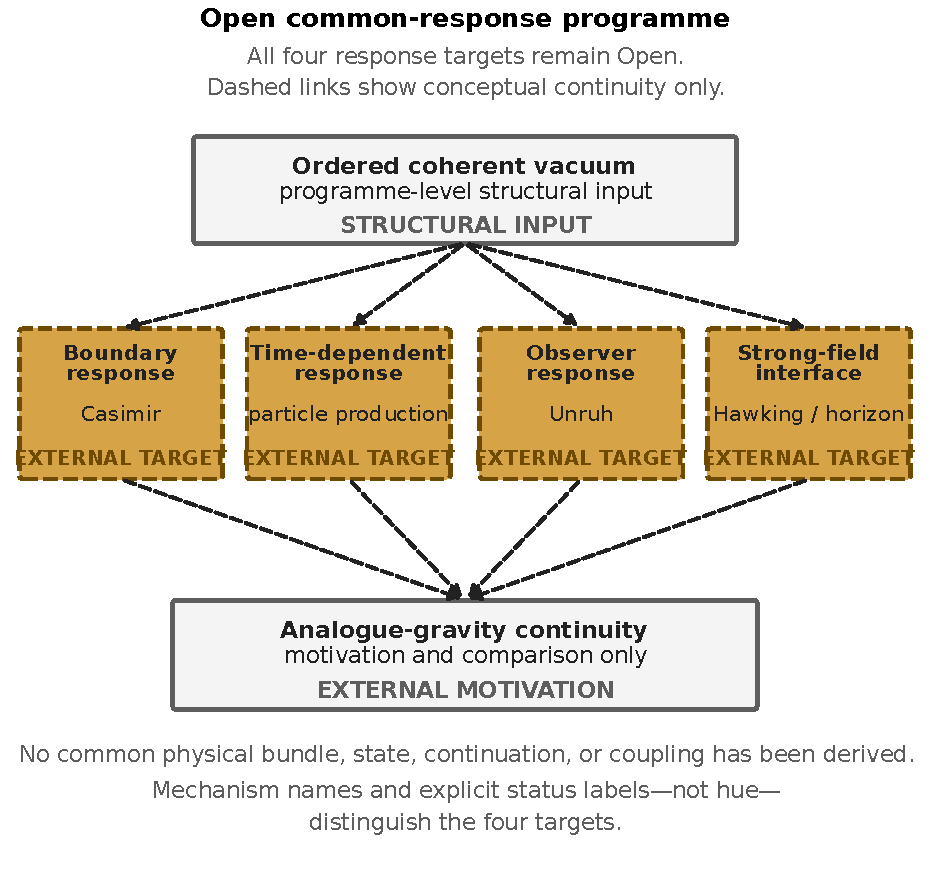
\includegraphics[width=\textwidth]{figures/r123/fig_qs_vacuum_unified_r123.pdf}
\caption{Open common-response programme for the quantum sector.  Boundary,
time-dependent, observer and strong-field responses remain four external
targets.  The shared gold fill marks the Open-status class.  All links are
dashed because no common physical ECT bundle, state, continuation and
coupling owning all four responses has been derived; analogue-gravity
continuity is motivation only.}
\label{fig:qs_vacuum_unified}
\end{figure}

\FloatBarrier
For a more extended structural discussion of the unified
vacuum-response logic and its analogue-gravity continuity, see
Appendix~\ref{app:qs_vacuum_response}.

% ============================================================
\subsection{Boundary sensitivity in a supplied vacuum model and the Casimir calculation}
\label{sec:qs_casimir}
% backward-compatibility alias:
\label{sec:casimir}
% ============================================================

\textit{Status: Level~A for the elementary Dirichlet boundary-value
calculation \emph{inside a supplied set of independent massless scalar
fields}.  Open~(OP-Q12, OP-Q18) for an ECT Casimir effect: the current
strict scalar map has one longitudinal coordinate rather than three
independent coordinates, while the physical mode count and boundary
coupling, mode multiplicity, renormalised stress tensor, force sign,
and laboratory implementation are not derived.
Connection: vacuum ontology
(\S\ref{sec:qs_vacuum_intro}), unified-response logic
(\S\ref{sec:qs_vacuum_unified}), medium character~(P5),
Goldstone counting from $O(4)\to O(3)$, analogue-laboratory
programme~(\S\ref{sec:analogue_lab}), and
Appendix~\ref{app:goldstone_integrability}.}

\medskip
An ordered medium can in principle respond to boundaries, but this
general possibility is not yet an ECT prediction of a measurable
Casimir force.  Such a prediction requires a physical boundary
operator that changes the spectrum of the reduced propagating bundle
and a derived stress observable.

\subsubsection*{Why a Casimir-type effect is expected}

If a supplied coherent-vacuum model supports fluctuation modes, then
imposing boundary conditions changes the allowed mode spectrum.
Schematically,
\begin{equation}
  \label{eq:qs_casimir_modes}
  E_{\rm vac}^{\rm(boundary)}
  \neq
  E_{\rm vac}^{\rm(free)}.
\end{equation}
In the supplied scalar toy problem the resulting energy difference
induces a force.  Whether a material boundary constrains the physical
$\Phi$-medium modes in this way is an additional, presently Open,
question.

\subsubsection*{ECT interpretation}

In ordinary QFT the Casimir force is often phrased as a consequence of
zero-point mode subtraction.
If a physical ECT boundary operator is derived, P5 would motivate
interpreting the corresponding energy difference as response of an
ordered medium rather than merely as formal mode subtraction.  The
present manuscript does not yet derive that operator.

\paragraph{Medium reading of boundary sensitivity~(P5).}
Under the medium interpretation~(P5), a future physical boundary map
could be read as deformation of a genuine ordered medium.  Only after
that map is known may one infer that the condensate between boundaries
has a modified physical spectrum or measurable stress.
This medium-level reading is conceptually continuous with superfluid
and analogue-vacuum Casimir phenomena, though it does not by itself
prove the quantitative ECT coefficient in any given laboratory setup.

\subsubsection*{Status and future derivation}

The present ECT action does not yet support a theorem asserting the
existence or coefficient of a physical condensate-sector Casimir
force.  It only motivates the boundary-response programme and supplies
a setting in which a future reduced action and boundary map can be
tested~(OP-Q12).

\statussummary
\textit{Established~(Level~A, supplied toy model only):}
the standard Dirichlet calculation for $N$ independent massless scalar
fields gives the algebraic expression~\eqref{eq:casimir_ect} below.

\textit{Open~(OP-Q12, OP-Q18):}
the value of $N$ in the physical reduced ECT bundle, the boundary
coupling, the completed coherent-vacuum stress calculation in realistic
geometries, and the identification of systems that realise the required
boundary conditions.

% ============================================================
\subsubsection{Supplied scalar Dirichlet boundary-value problem}


% -------------------------------------------------------------------------

\textbf{Scope and applicability (read before the formula).}
The calculation below is a supplied boundary-value toy model.  No
ordinary material, superfluid interface, BEC wall, or cosmological
phase boundary has been shown to impose its Dirichlet condition on the
physical ECT soft bundle.  In particular, neither transparency of
metals nor a purely gravitational coupling of that bundle follows from
the present action.

\subsubsection{Derivation inside the supplied scalar toy model}

\textbf{Boundary condition assumption.}
Dirichlet conditions and $N$ mutually independent massless scalar
fields are supplied as inputs.  They are not consequences of the
current ECT action.

For reference, the standard QED result for two photon polarisations
between parallel plates separated by $a$ is
\begin{equation}
  \frac{F}{A}\bigg|_{\rm QED}
  \;=\;
  -\frac{\pi^2}{240}\,\frac{\hbar c}{a^4}\,.
  \label{eq:casimir_qed}
\end{equation}
For $N$ supplied, independent, massless scalar fields with propagation
speed $c_{\rm toy}$ and ideal Dirichlet plates, the fields contribute
independently:
\begin{equation}
  \boxed{%
  \frac{F}{A}\bigg|_{N\,{\rm scalars}}
  \;=\;
  -\frac{N\pi^2}{480}\,\frac{\hbar c_{\rm toy}}{a^4}\,,
  }
  \label{eq:casimir_ect}
\end{equation}
which follows from zeta-function regularisation~\cite{BirrellDavies1982}:
\begin{equation}
  E_0^{\rm ren}(a) \;=\; -N\frac{\pi^2}{1440}\,\frac{\hbar c_{\rm toy}\,A}{a^3}
  \;\implies\;
  \frac{F}{A} = -\frac{\partial E_0^{\rm ren}}{\partial a}\bigg/A\,.
\end{equation}
Equation~\eqref{eq:casimir_ect} is standard toy-model algebra, not an
ECT force law.  The once-used substitution $N=3$ is not licensed by the
current integrable soft sector and is therefore not retained as a
prediction.  If three independent Dirichlet scalar channels are
\emph{supplied by hand} and $c_{\rm toy}=c$, the standard formula gives
$(F/A)_{N=3}/(F/A)_{\rm QED}=3/2$.  This arithmetic identity is retained
as a check of the toy BVP; it is not an ECT polarisation count or
laboratory prediction.

\paragraph{Soft-mode counting caveat.}
The supplied orientation target $O(4)/O(3)\simeq S^3$ carries three
coordinate directions in the unconstrained sigma-model parametrisation.
However, in the scalar-only integrable basis these do not
automatically correspond to three independent propagating soft
particles: the strict linear scalar map is parametrised by one longitudinal
coordinate~$\chi$ (Level~A kinematics;
Section~\ref{sec:goldstone_integrability_main},
Appendix~\ref{app:goldstone_integrability}).
The physical soft-mode count requires a supplied reduced action, quotient or
domain, and projector; $N_G^{\rm phys}=1$ is only a Level~B possibility inside
such a reduced EFT, not a consequence of integrability.
Therefore the earlier substitution of a three-component coordinate
count into a physical Casimir coefficient is invalid.  Even the
conditional physical mode represented by this coordinate cannot be inserted into
\eqref{eq:casimir_ect} until its material boundary coupling and stress
operator are derived.
This caveat applies equally to any use of the three-component count
in the dark-sector~(\S\ref{sec:dark_sector}) and particle-spectrum
sections.

\textbf{Summary statement and status caveat.}
Equation~\eqref{eq:casimir_ect} records only the supplied scalar
Dirichlet algebra.  ECT presently predicts neither a correction to the
electromagnetic metallic-plate force nor a distinct condensate-sector
coefficient for any laboratory setup.

\paragraph{Discriminant: laboratory QED Casimir versus ECT condensate
Casimir.}
Three cases must be kept sharply distinct.
\begin{enumerate}[label=(\roman*)]
  \item \textbf{Standard metallic-plate Casimir experiments:}
  these test the electromagnetic QED vacuum and do not by themselves
  test an ECT condensate sector, because no derived map shows that they
  impose boundary conditions on the
  soft ordered-branch sector.
  \item \textbf{Condensate-reflecting boundaries:}
  the supplied scalar calculation applies only after the number of
  independent fields and their Dirichlet coupling have been posited.
  No such physical ECT boundary model has yet been identified.
  \item \textbf{Intermediate analogue systems:}
  superfluid, BEC, domain-wall, or phase-boundary systems may probe the
  same boundary-sensitivity logic without reproducing the exact
  idealised Dirichlet setup assumed in the toy estimate.
  They motivate future boundary-response models but do not yet test a
  quantitative ECT prediction.
\end{enumerate}
The next theoretical gate is to derive a physical reduced boundary
operator and stress tensor before proposing a discriminating experiment.

\paragraph{Empirical anchor.}
The standard electromagnetic Casimir force has been measured with high
precision in metallic and related laboratory
setups~\cite{Lamoreaux1997,Bressi2002}.
These experiments do \emph{not} directly test an ECT condensate-sector
law, because no such law or material boundary map has yet been derived.
They establish boundary-sensitive QED vacuum response in their owning
theory.  For ECT they are only an external matching target; they neither
select ordered-medium ontology nor support an ECT boundary law.

\paragraph{Gate for the boundary-sensitivity programme.}
The programme advances only if a completed reduced ECT action yields a
boundary-coupled propagating bundle and a renormalised stress response.
Only then can a physical coefficient and falsifier be defined.
Standard metallic-plate Casimir experiments currently test QED, not a
derived ECT boundary law.

\paragraph{Connection to the analogue-laboratory and unified-response
programmes.}
Boundary sensitivity is the most direct and experimentally accessible
entry point into the unified vacuum-response logic developed in
Section~\ref{sec:qs_vacuum_unified}.
It is also the vacuum-response sector that lies closest to the
analogue-laboratory programme of Section~\ref{sec:analogue_lab}, where
phonon, superfluid, and BEC systems provide the most natural candidate
platforms for testing ordered-medium boundary response beyond the
purely electromagnetic Casimir effect.

\textbf{Programme-level connection.}
A future calculation may relate the boundary, detector, and
influence-functional correlators after their physical bundles, states,
and couplings are specified.  Their reduction to one universal ECT
correlator is a proposed programme, not a present result.

% -------------------------------------------------------------------------

% ============================================================
\subsection{Accelerated observers and the Unruh-type response}
\label{sec:qs_unruh}
% backward-compatibility alias:
\label{sec:unruh}
% ============================================================

\textit{Status: Level~A for the standard Rindler/KMS reconstruction
inside a supplied Lorentzian QFT state with a massless correlator and
an Unruh--DeWitt detector.  Open~(OP-Q12) as an ECT result: the physical
Lorentzian state, reflection positivity/analytic continuation,
detector coupling, physical cone, and the matching $S_0=\hbar$ have not
all been derived from the current $\Phi$-medium action.
Connection: vacuum ontology~(\S\ref{sec:qs_vacuum_intro}),
unified-response logic~(\S\ref{sec:qs_vacuum_unified}),
medium character~(P5), Euclidean $O(4)$ symmetry~(P2),
Casimir boundary sensitivity~(\S\ref{sec:qs_casimir}),
strong-field horizon response~(\S\ref{sec:qs_black_holes}),
and the analogue-laboratory programme~(\S\ref{sec:analogue_lab}).}

\medskip
The standard Unruh calculation demonstrates what a completed ECT
vacuum sector would have to reproduce.  It does not establish that the
current ordered-medium variables already define the required
Lorentzian QFT state and detector observable.

\subsubsection*{Kinematic expectation}

For uniform acceleration $a$, the standard QFT result gives
\begin{equation}
  \label{eq:qs_unruh_temp}
  T_U
  =
  \frac{\hbar\,a}{2\pi\,c\,k_B}.
\end{equation}
This formula uses the observed $\hbar$ and $c$.  In ECT the
identifications $S_0=\hbar$ and of a physical characteristic cone with
$c$ are matching conditions, not consequences of P1--P6.

\paragraph{Medium reading of the Unruh response~(P5).}
Under P5, a future completed ECT construction would interpret an Unruh
response as detector sampling of a genuine medium state.  The present
action has not yet shown that its Euclidean correlator reconstructs the
required physical Lorentzian state or that an accelerated detector
couples to it in the standard way.

\subsubsection*{ECT status}

An Unruh-type effect remains a target of the ordered-vacuum programme.
What is not yet in place is its detector-response derivation from a
completed ECT coherent EFT~(OP-Q12).

\statussummary
\textit{Established~(Level~A, supplied QFT assumptions only):}
the standard massless Wightman function restricted to a Rindler
trajectory satisfies the KMS condition and gives
\eqref{eq:unruh_ect}.

\textit{Open~(OP-Q12) for ECT:}
the physical state, continuation, cone and detector-response derivation
from the completed coherent EFT.  Direct experimental detection of the
Unruh effect also remains unsettled.

\paragraph{Observational status and empirical anchor.}
At present there is no universally accepted direct laboratory detection
of the Unruh effect itself.
Accordingly, ECT should not claim observational confirmation here.
Indirect discussions exist in the literature, for example in connection
with electron depolarisation in storage rings~\cite{Bell1983}, but such
arguments are not generally regarded as a clean standalone detection of
the Unruh effect.
The calculation below is therefore a conditional target and an
internal consistency test, not an ECT-specific empirical success.

% ============================================================
\subsubsection{Conditional correlator-based reconstruction of the Unruh response}

% -------------------------------------------------------------------------

\subsubsection{Derivation}

The derivation below is a conditional reconstruction using the standard
Euclidean correlator of a massless scalar/Goldstone-coordinate mode in a
supplied free Gaussian model, taken as a proxy for the completed soft coherent
sector.  It does not identify a physical ECT particle or derive
$m_\chi=0$.
It shows structural compatibility and continuity with the standard result,
not yet a full first-principles ECT derivation from the completed
coherent EFT.

The Unruh effect \cite{Unruh1976,Fulling1973,Davies1975} states that a
uniformly accelerated observer detects the Minkowski vacuum as a thermal
bath at $T_U = \hbar a/(2\pi k_B c)$.  In ECT this structural
reconstruction proceeds from the Euclidean correlator via analytic
continuation.

The Euclidean two-point function of that supplied massless scalar proxy is
\cite{BirrellDavies1982}:
\begin{equation}
  G_E(X,X')
  \;=\;
  \frac{1}{4\pi^2\,|X-X'|^2}\,,
  \qquad
  |X-X'|^2 \;=\; (\boldsymbol{x}-\boldsymbol{x}')^2 + (w-w')^2\,.
  \label{eq:green_euclidean}
\end{equation}

If the supplied Euclidean correlator satisfies the hypotheses needed
for reconstruction of a physical Lorentzian state, its continuation is
\begin{equation}
  G^+_M(x,x')
  \;=\;
  -\frac{1}{4\pi^2 c^2}
  \cdot
  \frac{1}{(t-t'-i\varepsilon)^2 - |\boldsymbol{x}-\boldsymbol{x}'|^2/c^2}\,,
  \label{eq:wightman}
\end{equation}
the standard Wightman function.  Invoking the
Osterwalder--Schrader theorem~\cite{OsterwalderSchrader1973} here is an
assumption about the supplied correlator and state; it is not yet a
proof that the present ECT Euclidean action satisfies all reconstruction
axioms.

Along the Rindler trajectory with proper acceleration $a$,
$G^+_M$ becomes periodic in imaginary proper time with period
$\beta_U = 2\pi c/a$ --- a thermal distribution.
The Unruh--DeWitt detector response gives a Planck spectrum with:
\begin{equation}
  \boxed{%
    T_U \;=\; \frac{\hbar\,a}{2\pi c\,k_B}\,,
  }
  \label{eq:unruh_ect}
\end{equation}
which is the standard result.  Replacing $c$ by a model characteristic
speed is not licensed until that speed is shown to be the physical
Lorentzian detector cone.  No accelerator number is quoted as an ECT
prediction because an accelerated proton is not an Unruh--DeWitt
thermometer and its response map has not been derived.

\subsubsection{Physical interpretation}

In a possible ECT completion, the Unruh effect would not be an
additional postulate about accelerated observers.  It would have to
follow from the physical continuation and detector sampling of the
ordered-medium state.  That completion is Open.
The Euclidean two-point function~\eqref{eq:green_euclidean} is
manifestly $O(4)$-invariant.
Under the supplied formal Euclidean--Lorentzian continuation, that
object is accessed through different Lorentzian decompositions:
inertial observers use the
standard Minkowski mode split, whereas uniformly accelerated observers
probe the same vacuum along Rindler trajectories.
The thermal character of the response is therefore not a new dynamical
heating of the vacuum, but a consequence of how the \emph{supplied}
Lorentzian state is sampled by the detector.  Ownership of that state
and detector by ECT remains Open.

This supplied-QFT calculation is mathematically analogous to the
Casimir boundary problem and the near-horizon Rindler target.  It does
not prove that one ECT correlator owns all three responses.
It is also consistent with the decoherence programme
(\S\ref{par:decoherence_programme}), though the present Unruh effect is
not itself a decoherence calculation and should not be reduced to
environmental tracing alone.

\paragraph{Connection to the unified vacuum-response programme.}
The Unruh response is one target of the unified vacuum-response
programme in Section~\ref{sec:qs_vacuum_unified}.  Establishing that it
shares a physical ECT operator and state with the boundary,
particle-production and black-hole sectors is an Open test of that
programme.

\paragraph{Discriminant: emergent versus assumed Unruh response.}
In standard Lorentzian quantum field theory, the Unruh effect is
derived after one has already assumed the quantum vacuum and its
Lorentzian analyticity properties.
ECT seeks to reverse that logical direction by deriving the physical
state and continuation from an ordered Euclidean medium.  The displayed
calculation shows the required endpoint but does not yet perform that
derivation.

\paragraph{Gate for the Unruh-response programme.}
Before an ECT-specific falsifier can be stated, the theory must derive a
reflection-positive Euclidean state, its physical Lorentzian
continuation and cone, and a detector coupling.  The completed model
must then reproduce the KMS temperature~\eqref{eq:unruh_ect}; failure
would reject that completion.

% ============================================================
\subsection{Cosmological particle production and time-dependent ordered backgrounds}
\label{sec:qs_particle_production}
% ============================================================

\textit{Status: A external/QFT mathematics for Bogoliubov mixing after
a time-dependent quadratic action, in/out states and particle basis are
supplied.  Open ECT for the physical time-dependent action, transition
history and clock, in/out vacua, particle observable, production rates
$|\beta_k|^2$, and primordial fluctuation spectrum.
Connection: vacuum ontology~(\S\ref{sec:qs_vacuum_intro}),
unified-response logic~(\S\ref{sec:qs_vacuum_unified}),
medium character~(P5), MP cosmology~(\S\ref{sec:mp_cosmo}),
the ordering-transition programme~(\S\ref{sec:qs_particle_production},
\S\ref{sec:ordering_gw}), and the analogue-laboratory
programme~(\S\ref{sec:analogue_lab}).}

\medskip
If the ordered condensate background changes in time, the notion of
``particle'' defined relative to one coherent vacuum slicing need not
coincide with that defined relative to another.
This is a standard candidate setting for cosmological particle production,
complementary to the macroscopic transition programme
of Section~\ref{sec:mp_cosmo}.

\paragraph{Physical picture: particle creation as vacuum
reconfiguration.}
If a completed ECT transition supplies the required time-dependent
quantum action and states, particle creation can be read as a change of
excitation content rather than ``appearance from nothing''.
This is entirely analogous to the physics of known media: rapidly
cooling a superfluid produces phonons and rotons not because they
``materialise from the void'', but because the background against
which ``silence'' is defined has changed.
Whether the resulting excitations are physical ECT particles, and their
number and spectrum, depends on the missing action, state, detector and
transition-history maps.

\subsubsection*{Time-dependent ordered branch}

In a nonstationary background, the effective coherent vacuum is itself
time-dependent.
Mode decomposition at early and late times therefore differs.
Schematically, the early-time and late-time mode operators are related
by a Bogoliubov transformation,
\begin{equation}
  \label{eq:qs_bogoliubov}
  a_k^{\rm(out)}
  =
  \alpha_k\,a_k^{\rm(in)}
  +
  \beta_k\,a_{-k}^{\rm(in)\dagger},
\end{equation}
with $|\beta_k|^2$ measuring the produced excitation density.
This is A mathematics for a supplied quadratic QFT problem.  It is not
yet an ECT result: the actual $\alpha_k$, $\beta_k$ and their particle
interpretation require the completed time-dependent action and in/out
state construction.

\subsubsection*{ECT interpretation}

Conditional on those owners, particle production would be a
reorganisation of excitation content relative to a changing ordered
background.  This is an interpretation target, not a derived event in
the present ECT history.

\paragraph{Medium reading of particle production~(P5).}
Under the medium interpretation~(P5), a future particle-production
completion would be read as reorganisation of excitation content within
an ordered medium whose physical background configuration changes in
time.
What standard curved-spacetime QFT describes as particle creation in a
time-dependent geometry, the ECT programme would read as mode redistribution
in one candidate ordered medium whose effective parameters evolve during a
separately supplied physical history.  No ordering transition is derived.

\paragraph{Empirical anchor.}
Time-dependent particle production is not a speculative mechanism.
Bogoliubov-type mode mixing is standard in nonstationary quantum-field
settings, and closely related laboratory logic has been observed in the
dynamical Casimir effect~\cite{Wilson2011}.
ECT does not yet claim a completed first-principles derivation of
cosmological production rates from condensate dynamics.
The present text records compatibility with that external formalism and
the precise missing owners; it does not claim a produced ECT population.

\subsubsection*{Relation to MP cosmology}

Macroscopic Physics describes the large-scale evolution of the ordered
branch (Section~\ref{sec:mp_cosmo}).
The present QS subsection gives the coherent-vacuum interpretation of
how such time dependence can populate excitation sectors.
The two descriptions are complementary: MP governs the background
history; QS governs excitation production against that history.

The most important application is the
$O(4)\to O(3)$ ordering transition itself
(\S\ref{sec:qs_particle_production}).
If that transition is non-adiabatic in a derived physical quadratic
mode action, it can generate Bogoliubov mixing.
The resulting coefficients are relevant in principle for
(i)~the primordial fluctuation spectrum,
(ii)~the initial excitation content of the ordered branch,
and (iii)~the ordering-transition gravitational-wave programme
(\S\ref{sec:ordering_gw}).
The external Bogoliubov framework is stated here as the target; both
its ECT ownership and the quantitative completion belong to the Open
cosmological programme of Part~II.

\statussummary
\textit{Established externally~(A mathematics):}
given a time-dependent quadratic action and two specified positive-
frequency splittings, Eq.~\eqref{eq:qs_bogoliubov} is the standard
canonical transformation.

\textit{Open~ECT (OP-Q12, OP3):}
the time-dependent physical action, transition history and clock,
in/out states, particle map, production rates $|\beta_k|^2$, and the
primordial fluctuation spectrum.

\paragraph{Discriminant: time-dependent ordered-medium production versus
postulated vacuum particle creation.}
In standard curved-spacetime QFT, cosmological particle production is
derived once one has already assumed a quantum vacuum on a given
time-dependent background.
In ECT the ordered medium is primary, and the changing background is a
change of the condensate state itself.
The mathematics of Bogoliubov mixing is continuous with the standard
treatment, but the ontological reading is reversed:
the ``vacuum'' is not a passive background on which particles appear,
but the physical medium whose nonstationary evolution reorganises its
own excitation content.

\paragraph{Falsifier for the particle-production programme.}
The programme passes only if a completed ECT transition produces a
positive, stable time-dependent mode action, well-defined in/out states
and particle observables, and an excitation history compatible with the
background and primordial data.  Failure rejects that completion; the
generic external Bogoliubov identity is not itself an ECT prediction.

\subsubsection{Vacuum-response target table}
\label{sec:vacuum_summary_tables}

{\small
\begingroup
\setlength{\tabcolsep}{5.69pt}
\begin{longtable}{@{}L{3.3cm}L{3.0cm}L{2.8cm}L{2.8cm}L{2.5cm}@{}}
\caption{Supplied QFT response calculations used as targets for a future ECT vacuum completion.  ``A mathematics'' refers only to the stated external/toy assumptions; all physical ECT owners listed here remain Open.}\label{tab:vacuum_predictions}\\
\toprule
Effect & Supplied/external formula & ECT disposition & Standard result & Status \\
\midrule
\endfirsthead
\toprule
Effect & Supplied/external formula & ECT disposition & Standard result & Status \\
\midrule
\endhead
\bottomrule
\endfoot
Supplied $N$-scalar Dirichlet BVP &
$-\dfrac{N\pi^2\hbar c_{\rm toy}}{480 a^4}$ &
No ECT force coefficient &
Standard scalar BVP & A mathematics / Open ECT \\
Standard Unruh target &
$\dfrac{\hbar a}{2\pi c k_B}$ &
No ECT detector prediction &
$\dfrac{\hbar a}{2\pi c k_B}$ & A external / Open ECT \\[8pt]
Particle production in time-dependent background &
$a_k^{\rm(out)}=\alpha_k a_k^{\rm(in)}+\beta_k a_{-k}^{\rm(in)\dagger}$ &
No ECT particle rate or state map &
Bogoliubov mixing & A external / Open ECT \\
Standard Hawking target &
$T_{\rm H}=\dfrac{\hbar \kappa}{2\pi c k_B}$ &
Physical ECT tensor geometry, state and strong-field response Open &
Standard semiclassical-QFT form & A external / Open ECT \\
\bottomrule
\end{longtable}
\endgroup
}

\paragraph{Status note on the horizon-thermality row.}
The Hawking row is a standard target, not an ECT derivation.  A physical
tensor metric, horizon state, continuation and strong-field response
operator are all missing from the current completion.


% -------------------------------------------------------------------------

Parker \cite{Parker1969} showed how time-varying supplied backgrounds can
produce particle pairs.  The ECT $O(4)\to O(3)$ transition history,
physical clock and duration are not derived; in particular no
Planck-time transition estimate is retained.

For a separately supplied scalar quadratic mode $v_k$, the standard
oscillator target is~\cite{Parker1969,BirrellDavies1982}:
\begin{equation}
  \ddot{v}_k + \Omega_k^2(t)\,v_k \;=\; 0\,,
  \qquad
  \Omega_k^2(t) \;=\; c_{\rm char}^2(t)\,k^2 + m_{\rm eff}^2(t)\,,
  \label{eq:mode_equation}
\end{equation}
where $c_{\rm mode}(t)$ and $m_{\rm mode}^2(t)$ are supplied functions
of the chosen background.  Using the established equation label, we
write them as $c_{\rm char}(t)$ and $m_{\rm eff}(t)$ in
Eq.~\eqref{eq:mode_equation}; neither function is derived for a physical
ECT transition.  Scalar integrability leaves one longitudinal coordinate in
the strict map, not three independent $\pi^i$ coordinates; the physical mode
count remains conditional on the supplied action and projector.

\paragraph{Candidate time-dependent mode speed.}
Equation~\eqref{eq:mode_equation} allows a supplied mode speed
$c_{\rm char}(t)$ to enter as a time-dependent parameter.
In standard particle-production treatments on a fixed Lorentzian
background, the speed of light is constant and non-adiabaticity enters
through the background geometry or effective masses alone.
In a future ECT completion, the ordered medium may carry additional
time dependence during the transition through parameters that set
$c_{\rm char}(t)$.
This is a possible source of mode mixing, not a currently derived
ECT-specific effect.  Its existence and quantitative importance belong
to the completed transition-history calculation.

The expected particle number per mode is
$\mathcal{N}_k = |\beta_k|^2$,
where $\beta_k$ are Bogoliubov coefficients \cite{BirrellDavies1982}.
An ECT-native computation of $n_s$ and $r$ from the condensate
fluctuation spectrum during the ordering transition remains
open~(OP3, \S\ref{sec:mp_primordial}).

% -------------------------------------------------------------------------

\paragraph{Discriminant with respect to standard vacuum programmes.}
ECT differs from the standard presentation of vacuum phenomena in one
central respect:
Casimir response, Unruh response, particle production, decoherence, and
horizon thermality are compared as candidate probes of one ordered
medium.  This is an Open hypothesis, not a derived equivalence.  The
theory seeks a single condensate correlator
infrastructure behind boundary response, detector response,
nonstationary production, and open-system decoherence.
If this unified correlator logic fails, the vacuum-response
programme fails as a whole rather than piecemeal.

\paragraph{Falsifier for the coherent-vacuum response programme.}
The present vacuum-response programme would be seriously weakened if the
different sectors ultimately required mutually unrelated vacuum
structures:
for example, if Casimir-type boundary response required one underlying
vacuum, Unruh response another, particle production a third, and
decoherence kernels a fourth.
It would also be weakened if a completed coherent EFT showed that no
single ordered-vacuum correlator can jointly support boundary
sensitivity, accelerated-detector response, nonstationary mode mixing,
and the horizon thermality route.
Conversely, a successful cross-link would show only that one specified
source-model kernel can reproduce the named effects.  It would support ECT
only after an independently derived ECT correlator and observable bridge are
identified.

\paragraph{External mechanisms, not ECT evidence.}
The following empirical or standard-theory facts belong to their own source
models:
the success of standard QED Casimir measurements for electromagnetic
boundaries, the observed dynamical Casimir effect in driven effective
boundary systems~\cite{Wilson2011}, the standard consistency of Bogoliubov-type particle
production in nonstationary backgrounds, and the broad analogue-gravity
continuity between detector response, horizon thermality, and
effective-vacuum physics.
They establish neither a common correlator nor an ECT bridge and therefore
are not confirmations, support, or consistency evidence for the
ordered-vacuum interpretation.

\subsection{Summary and status of coherent-vacuum response}
\label{sec:qs_vacuum_summary}
% ============================================================

\textit{Status: summary subsection for the coherent-vacuum programme
of Chapter~\ref{sec:qs_vacuum_response}.
Collects the Level~A structural claims, the Level~B conditional or
closure-dependent results, and the open quantitative programmes.
The chapter-level discriminant, falsifier, and empirical anchors are
developed in Section~\ref{sec:qs_particle_production}.}

\begin{longtable}{@{}L{6.7cm}L{2.7cm}L{5.1cm}@{}}
\caption{Coherent-vacuum response map of ECT.
Level~A = exact in the declared model and assumptions, with an explicit reproducible derivation; reproducible checks verify
that derivation but do not replace it; it does not by itself establish descent from P1--P6 or
physical ECT ownership.
Level~B = structural/conditional derivation or closure route with a
declared open matching, input, or identification step.
Open = not yet derived; OP-Q reference given.} \\
\label{tab:qs_vacuum} \\[-6pt]
\toprule
Vacuum-sector statement & Status & Basis / comment \\
\midrule
\endfirsthead
\toprule
Vacuum-sector statement & Status & Basis / comment \\
\midrule
\endhead
\midrule\multicolumn{2}{r}{\small\textit{(continued on next page)}}\\
\endfoot
\bottomrule
\endlastfoot
Supplied coherent-vacuum model has nontrivial correlators
  & Level~A within the declared model / Open ECT owner
  & Model-internal state and correlator statement;
    Section~\ref{sec:qs_vacuum_intro} \\
Phase-sensitive vacuum response in the supplied coherent sector
  & Level~A within the declared model / Open ECT owner
  & Requires BR1 and the separately supplied state and action;
    Section~\ref{sec:qs_vacuum_intro} \\
Physical medium ownership of the vacuum-response programme~(P5)
  & Level~B/Open
  & P5 motivates relational medium response but does not derive a common
    physical vacuum, state or correlator owner;
    Section~\ref{sec:qs_vacuum_intro} \\
Supplied soft-sector boundary-value response
  & Level~A mathematics / B--Open physics
  & Each declared operator and boundary condition has a calculable mode
    response; the physical condensate boundary and its coupling to ordinary
    matter are not derived; Section~\ref{sec:qs_casimir} \\
Supplied scalar Dirichlet coefficient
  & Level~A mathematics / Open ECT
  & Eq.~\eqref{eq:casimir_ect}; physical ECT mode count, boundary
    coupling and stress response are missing \\
Time-dependent ordered backgrounds: background-dependent particle notion
  & A external / Open ECT
  & Standard statement after a time-dependent action and in/out states are supplied;
    Section~\ref{sec:qs_particle_production} \\
Bogoliubov-type mode mixing in the coherent vacuum
  & A external / Open ECT
  & Eq.~\eqref{eq:qs_bogoliubov}; ECT action, states, particle map and rates remain open;
    Section~\ref{sec:qs_particle_production} \\
Candidate time-dependent mode speed $c_{\rm char}(t)$
  & Open
  & Supplied function in the displayed oscillator target; its physical
    ECT owner and quantitative importance are not derived;
    Section~\ref{sec:qs_particle_production} \\
Quantitative production rates $|\beta_k|^2$
  & Open (OP-Q12)
  & Requires completed time-dependent coherent-vacuum calculation \\
Euclidean--Rindler/KMS route
  & Level~B/Open
  & The standard response follows only after supplying the physical metric,
    state/KMS condition, detector coupling and clock/action matchings;
    Section~\ref{sec:qs_unruh} \\
Unruh temperature formula in the supplied route
  & Level~A external / Open ECT
  & Eq.~\eqref{eq:unruh_ect}; requires $S_0=\hbar$, a physical cone,
    and the missing detector/state owners;
    Section~\ref{sec:qs_unruh} \\
Common vacuum-response programme (Casimir/production/Unruh/horizon)
  & Open
  & Section~\ref{sec:qs_vacuum_unified}; a proposed common architecture,
    not a single physical response operator derived for all four regimes \\
Analogue-gravity continuity of the ECT vacuum interpretation
  & Motivation / Open ECT
  & Section~\ref{sec:qs_vacuum_unified} \\
Unified coherent-vacuum response map
  & Open programme map
  & Fig.~\ref{fig:qs_vacuum_unified};
    Section~\ref{sec:qs_vacuum_unified} \\
Horizon thermality as a coherent-vacuum response channel
  & A external / Open ECT
  & Standard near-horizon target; physical ECT tensor geometry, state
    and strong-field response are missing;
    Section~\ref{sec:qs_black_holes} \\
Phase--action--quantization structural chain
  & Level~B
  & Sections~\ref{sec:qs_phase_dynamics}--\ref{sec:qs_born};
    Fig.~\ref{fig:qs_quantization_chain} \\
Unified vacuum/coherent/geometry interpretation
  & Level~B
  & Shared MP--QS condensate foundation \\

\end{longtable}

\paragraph{Summary.}
The coherent-vacuum programme of Chapter~\ref{sec:qs_vacuum_response}
now has a clear three-layer structure.

First, supplied reduced models define calculable correlators and
stiffnesses.  Physical boundary sensitivity, detector response and
strong-field ownership remain Open.

Second, treating Casimir, Unruh, particle-production and horizon
thermality as regimes of one common ECT operator is an Open organising
hypothesis.

Third, the chapter has identified which parts of this architecture are
already structural, which are conditional on specific closures, and
which remain open quantitative programmes.

In this sense, Section~\ref{sec:quantum_vacuum} presents an Open map
linking four supplied calculations.  Section~\ref{sec:qs_open_systems}
separately studies declared environmental reductions; equality of its
kernel with the boundary, detector or horizon kernels is not assumed.

% ============================================================

% ==============================================================
\section{Open Quantum Systems, Decoherence, and Irreversibility}
\label{sec:qs_open_systems}
% ==============================================================


\textit{Inputs: coherent amplitude structure, a supplied causal retarded
response, and the ordered-vacuum sector.  Status: Level~A conditional
mathematics for retarded support and for a nonnegative spectral/noise
quadratic only after the corresponding positive Hilbert/state/observable,
residue or oscillator representation is supplied; Level~B for generic
influence-functional bookkeeping in a specified Gaussian model; Open for the
ECT system--environment split, physical record operators, state-dependent
spectral/noise owner, entropy-production theorem, and unique outcome rule.}

\paragraph{Physical picture: reduced-state records.}
\label{par:decoherence_programme}
Tracing unresolved degrees of freedom can suppress interference and stabilise
pointer records.  This is a statement about a reduced density operator, not
selection of one ontologically realised branch.  The unresolved sector may
ultimately be part of the same condensate, but its coupling, state, and
coarse-graining must be derived rather than inferred from that ontology.


\paragraph{What is established, what is closure-dependent, and what
remains open in the decoherence programme.}

Established results are restricted to the declared source model:
causal retarded support and a positive pairwise noise quadratic.  The ECT
split, vertices, state, entropy theorem, and outcome update remain Open.
\paragraph{Recoherence.}
Finite or engineered environments can erase or refocus records and partially
restore off-diagonal terms.  The amount of recovery is computed from the
specified influence functional or channel.  No universal reverse/forward
probability follows from the pairwise decoherence exponent.

\paragraph{Connection to PES-R.}
The causal retarded kernel determines admissible modes and their pole
structure; the positive noise kernel determines pairwise record
distinguishability.  PES-R keeps these roles separate.  A one-history
translation susceptibility can be a declared robustness diagnostic, but it
is not the generic Feynman--Vernon mean equation.  Figure~\ref{fig:qs_decoherence_regimes}
summarises this channel-specific regime split without assigning an outcome.

\begin{figure}[htbp]
\centering
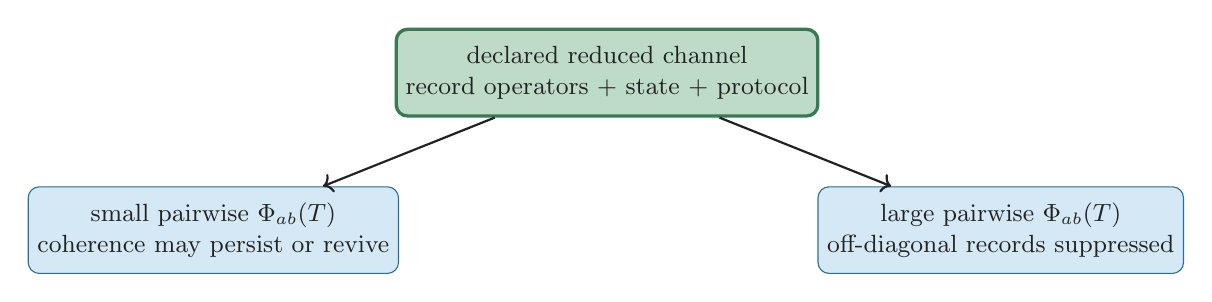
\begin{tikzpicture}[
  box/.style={draw,rounded corners,align=center,minimum width=4.0cm,
    minimum height=1.1cm,font=\small},
  arrow/.style={->,thick,draw=ectInk}]
\node[box,ectConditional] (channel) at (0,0)
  {declared reduced channel\\record operators + state + protocol};
\node[box,ectDerived] (weak) at (-5.0,-2.0)
  {small pairwise $\Phi_{ab}(T)$\\coherence may persist or revive};
\node[box,ectDerived] (strong) at (5.0,-2.0)
  {large pairwise $\Phi_{ab}(T)$\\off-diagonal records suppressed};
\draw[arrow] (channel) -- (weak);
\draw[arrow] (channel) -- (strong);
\end{tikzpicture}
\caption{Conditional reduced-state regime split.  The result is controlled by
the physical record differences and noise kernel, not by the total number of
environmental degrees of freedom alone.  Neither branch changes metric
signature or selects one realised outcome.  Green marks the declared
conditional channel and blue marks consequences inside it; labels and borders
carry the same information in grayscale.}
\label{fig:qs_decoherence_regimes}
\end{figure}

\medskip


\subsection{Influence functional, decoherence, and the arrow of time}
\label{sec:qs_decoherence}\label{sec:influence_functional}\label{sec:second_law}

\textit{Status: Level~A conditional mathematics within a declared
quadratic source model for causal retarded support and for spectral/noise
positivity when a positive state/observable/residue or oscillator
decomposition is supplied; Level~B as generic influence-functional
bookkeeping after a specified split; Open for the ECT split, vertices,
state/spectral/noise owner, entropy theorem, and outcome update.}


\paragraph{Position within the full argument.}

This programme follows the amplitude and causal-sector analysis
but does not retroactively derive it.  It classifies reduced records only
after the physical modes and couplings are known.

\paragraph{Relation to ECT Foundations.}

The foundational ontology suggests that resolved and unresolved
degrees of freedom may belong to one condensate.  That statement does not
identify the trace, state, record operator, or kernel required for a reduced
dynamics.

\subsubsection*{Why decoherence belongs to the coherent branch}

Decoherence is discussed in the coherent branch because it acts
on interference between coherent alternatives.  It suppresses selected
off-diagonal records; it neither creates the branch nor chooses one actual
outcome.

\paragraph{Discriminant with respect to standard decoherence and
arrow-of-time programmes.}

The discriminating task is not to reproduce generic decoherence
but to derive the ECT-specific record channel and a held-out deviation.  An
unspecified large environment is not an ECT prediction.

\paragraph{Medium reading of decoherence~(P5).}

P5 motivates a medium interpretation of the unresolved sector.
The quantitative content still comes from a declared interaction vertex,
state, and reduced map.

\paragraph{Connection to the global/reduced unitarity distinction.}

Fine-grained unitary or reflection-positive reconstruction and
reduced non-unitary evolution are compatible descriptions at different
levels.  Their compatibility does not furnish a unique-outcome rule.

\paragraph{Connection to the unified vacuum-response infrastructure.}

Vacuum-response calculations and reduced-state records may share
physical modes, but this creates a double-counting obligation rather than an
automatic identification of kernels.

\subsubsection*{Influence-functional form of the effective description}

For a declared Gaussian split one must also specify the joint initial
preparation and closed-time-path contour.  After centring the unresolved
one-point function, a compatible factorised preparation is sufficient for
the usual bulk decomposition.  Initial system--environment correlations
instead require an explicit initial-boundary term $S_{\rm ic}$, an equivalent
extended-contour construction, or a proof that the extra contribution
vanishes or has been absorbed consistently.  The bulk influence functional
then separates retarded response from a Hermitian noise quadratic.  Their
normalisations are fixed by
Eqs.~\eqref{eq:pes_fourier_dictionary}--\eqref{eq:pes_Phi_dictionary};
they are not interchangeable.

\paragraph{Status.}

The bulk quadratic influence-functional algebra is Level~A in the stated
source model and Level~B as generic bookkeeping, conditional on the declared
initial preparation and contour.  The correlated initial-boundary term and
ownership of the complete functional by the bare ECT action remain Open.

\subsubsection*{Causal retarded kernel: the Level~A result}

The retarded kernel satisfies $D^R(\tau<0)=0$ in the owning
hyperbolic construction.  This is a causality statement, not an entropy sign
or outcome-selection theorem.

\paragraph{Physical meaning.}

Retarded response fixes how a perturbation propagates, whereas the
noise kernel fixes pairwise record loss.  Even in equilibrium their relation
requires the state and fluctuation--dissipation assumptions.

\paragraph{Beyond the quadratic sector.}

Beyond a Gaussian truncation, higher cumulants and non-linear
vertices must be retained.  Positivity of the quadratic term alone does not
control the full non-Gaussian influence functional.

\subsubsection*{Low-entropy coherent initial sector}

A coherent initial sector is not automatically a low-entropy
sector.  The initial density operator and coarse-graining must be supplied;
P4 supplies the orientation datum, not a thermodynamic boundary condition.

\paragraph{Structure of the initial sector.}

The initial-sector structure must be stated through its state,
constraints, and physical modes.  Neither one realised orientation nor high
coherence determines its statistical entropy.

\subsubsection*{Path-integral weighting and the initial coherent sector}

A supplied Euclidean weight $e^{-\mathcal I_E^\mu}$ defines a
measure only after its domain, boundary data and normalisation are supplied;
for P3 the exponent is
$\kappa_{\rm P3}\mathcal I_E^{\rm P3}$.  It is neither fixed by $S_0$ nor a
Boltzmann probability distribution for macroscopic entropy.

\paragraph{Status.}

The path-integral expression is retained as amplitude
bookkeeping.  Its conversion into a physical initial ensemble remains an
Open reconstruction/state problem.

\subsubsection*{Conditional spectral positivity and dissipative kernel}

A nonnegative spectral measure supports a positive pairwise noise quadratic
only after its physical Hilbert space or oscillator decomposition, state,
observable, normalisation and residues have been supplied.  Causal dispersion
relations additionally require the retarded analyticity, Fourier and
subtraction conventions.  A classical positive scalar Hamiltonian and
retarded support do not derive those spectral owners.  The conditional
spectral algebra is Level~A under the stated premises; its ECT identification
is Open, and it implies neither Markovianity nor entropy monotonicity.

\subsubsection*{Effective ohmic regime and Markov approximation}

An ohmic spectrum and short memory are model assumptions useful
for a Markov approximation.  The corresponding coefficients must be derived
for each physical channel; they are not universal condensate constants.

\subsubsection*{Qualitative monotonicity of entropy}

Finite environments can exhibit recoherence, and even Markovian channels need not
increase von Neumann entropy unless the required channel property is stated.

\paragraph{Why this is enough.}

Causal support plus positive noise is enough for a consistent
quadratic record model, not for a thermodynamic theorem.  The stronger claim
requires the missing reduced-map hypotheses.

\paragraph{Status.}

Accordingly, the entropy-growth programme remains Open for ECT.
Only conditional channel theorems may be used before the physical reduction
is derived.

\subsubsection*{Working explicit entropy formula}

The applicable explicit relation is the contractive relative-entropy inequality for a named
channel and stationary reference state; no universal scalar rate is retained.

\paragraph{Role of the explicit formula.}

The conditional formula is a diagnostic of an already specified
channel, not a derivation of that channel from the condensate or a numerical
ECT prediction.

\subsubsection*{Macroscopic irreversibility versus quantum exception}

Macroscopic irreversibility and quantum recoherence can coexist
because different environments and timescales define different reduced
channels.  No sharp universal boundary follows from an order-unity scalar.

\paragraph{Numerical illustration.}

Any numerical illustration of a Markov source model is labelled
model-internal.  It cannot be promoted to an ECT lifetime or entropy rate
without the ECT vertex and state.

\paragraph{Interpretive consequence.}

The interpretation is therefore conditional: large pairwise
record exponents suppress selected coherences, while actual outcomes and
thermodynamic irreversibility remain separate questions.

\paragraph{Status.}

The quantitative example is retained only as a source-model
illustration.  It is not an experimental verification of an ECT kernel.

\subsubsection*{Bridge to probability and Born-type interpretation}

Decoherence can make a reduced density matrix approximately
diagonal but does not derive Born weights or select one realised outcome.
Ordinary projector Gleason represents only an independently supplied
normalised, noncontextual, countably additive projector measure on a complex
Hilbert space with $\dim\mathcal H\ge3$; a qubit requires the Busch effect/POVM theorem under separately declared C2q hypotheses.  It does not derive the physical state,
preparation, event, probability origin, outcome or update.

\paragraph{Falsifier for the decoherence and thermodynamic-arrow
programme.}

Falsification requires a derived ECT record operator and kernel:
if their predicted channel conflicts with held-out interference or
recoherence data, that channel fails.  Generic agreement with standard
decoherence is not discriminating.

\paragraph{External source-model anchors only.}

C$_{60}$, cavity, qubit, and photonic experiments are empirical
anchors for their source models.  Reproducing those models checks arithmetic
and conventions, not ECT-specific ownership.

\paragraph{Conditional cross-protocol consistency test for a future ECT
record channel.}

The conditional consistency requirement is this: once ECT fixes a vertex and
state, the same kernel must account for multiple protocols without
channel-by-channel retuning.  Until then the statement is a test plan, not a
prediction.

\paragraph{Connection to the structural universalities.}

Causal response, compact phase, and reduced records are distinct
structural ingredients.  Their coexistence does not license a universal
selection functional.

\paragraph{Summary.}

The decoherence architecture is thus a reproducible framework for
named channels, with ECT-specific vertices and states still Open.  Outcome,
Born, and entropy claims are not included in its established core.

\paragraph{Medium reading~(P5).}

P5 can motivate that apparatus and environment are excitations of
one medium, but it does not eliminate the need for a physical tensor product
or algebraic subsystem split.

\paragraph{Relation to the general decoherence programme.}

The general programme retains finite-time recoherence, null spaces,
and state dependence.  A universal monotone scalar is neither required nor
derived.
For two alternatives $a,b$, a declared Gaussian environment, and a named
joint initial preparation, a nonzero normalised scalar influence functional,
when it exists and includes all initial-boundary terms, has the branch-free
exact polar decomposition
\begin{equation}
  \mathcal F[a,b]
  =U_{ab}^{\rm full}\exp\!\left\{-\Xi_{ab}^{\rm full}\right\},
  \qquad
  U_{ab}^{\rm full}:=\frac{\mathcal F[a,b]}{|\mathcal F[a,b]|}\in U(1),
  \qquad
  \Xi_{ab}^{\rm full}:=-\ln|\mathcal F[a,b]| .
  \label{eq:qs_influence}
\end{equation}
On a domain where $U_{ab}^{\rm full}$ admits a chosen continuous real phase
lift one may write
$U_{ab}^{\rm full}=\exp(i\Theta_{\rm IF}^{\rm full})$, with the dimensionless
$\Theta_{\rm IF}^{\rm full}$ defined modulo $2\pi$; no global lift is implied.
If a separate reduction derives an action-valued real influence functional,
one may then define
$S_{\rm IF}^{R}:=S_0\Theta_{\rm IF}^{\rm full}$ modulo $2\pi S_0$.
That additional action owner and the cross-sector normalisation of $S_0$ are
not assumed by the polar decomposition.
This full quantity is a nonnegative suppression exponent only when the
declared reduced construction also establishes $|\mathcal F|\leq1$; only
then do we set $\Phi_{ab}:=\Xi_{ab}^{\rm full}\geq0$.  For a
compatible factorised preparation the displayed exponent can reduce to the
nonnegative bulk Gaussian noise quadratic of Result~A5.  For a correlated
preparation it may also contain initial-boundary contributions and cannot be
reconstructed, assigned a sign, or promoted to $\Phi_{ab}$ from the bulk
kernel $N$ alone.
The causal response kernel satisfies
\begin{equation}
  D^{R}(\tau<0)=0,
  \label{eq:qs_retarded_zero}
\end{equation}
under the owning hyperbolic/retarded construction.  Positivity of the
quadratic spectral measure,
\begin{equation}
  \rho(\mu^2)\ge0,
  \label{eq:qs_rho_positive}
\end{equation}
supports a positive noise quadratic; it does not imply entropy monotonicity.

The Euclidean weight
\begin{equation}
  Z_E=\int\mathcal D\Phi\,e^{-\mathcal I_E^\mu[\Phi]},
  \qquad
  \mathcal I_E^\mu=\kappa_{\rm P3}\mathcal I_E^{\rm P3}
  \quad\text{only for the supplied bare P3 measure},
  \label{eq:qs_partition_function}
\end{equation}
does not by itself prove that the realised ordered branch is a low-entropy
initial ensemble.  That requires a measure, coarse graining, and state
selection and remains Open.

For a declared three-dimensional derivative-coupling toy, the bare
mode-density weight and the Weiss spectral density are related by
\begin{equation}
  J_{\rm bare}(\omega)
  \propto N_{\rm eff}\omega^2|g(\omega/c_{\rm char})|^2
  \sim N_{\rm eff}\omega^4,
  \qquad
  J_W(\omega)\equiv\frac{J_{\rm bare}(\omega)}{2\omega}
  \sim N_{\rm eff}\omega^3,
  \label{eq:qs_super_ohmic}
\end{equation}
whereas the effective ansatz
\begin{equation}
  J_W(\omega)\simeq N_{\rm eff}\gamma\omega
  \label{eq:qs_ohmic}
\end{equation}
and the short-memory condition
\begin{equation}
  \tau_{\rm env}\ll\tau_{\rm dyn}
  \label{eq:qs_markov}
\end{equation}
are model inputs, not consequences of the minimal ECT bath.  Even together
they do not fix the sign of von Neumann entropy.  For a declared contractive
channel with stationary state $\rho_*$,
\begin{equation}
  \frac{d}{dw}D(\rho_w\Vert\rho_*)\le0,
  \label{eq:qs_entropy_monotone}
\end{equation}
while for a general derived generator $\mathcal L_w$ one only has
\begin{equation}
  \frac{dS_{\rm vN}}{dw}
  =-\operatorname{Tr}[\mathcal L_w(\rho_w)\ln\rho_w],
  \label{eq:qs_entropy_explicit}
\end{equation}
whose sign must be proved from the channel and state.

In a specified open-system model, macroscopic irreversibility can emerge
when uncontrolled records make recoherence operationally inaccessible, while
echo/control protocols show that the statement is finite-time and
channel-dependent.  A declared dephasing channel may establish reduced-state
record formation inside that model; it does not give a unique outcome, Born
weights, a metric-signature transition, or a Crooks relation.  The physical
ECT record operators, state, kernels, trace, entropy functional, and update
rule remain OP-Q5/OP-Q17/OP-Q19 inputs.

\subsection{Decoherence timescale in supplied external source models}
\label{sec:tau_ECT_systems}


\textit{Status: standard source-model definition for declared reduced
channels; Open for an ECT-specific rate.  A decoherence time is computable
only after the physical alternatives, record operator, environmental state,
noise kernel, protocol, and full-channel contractivity have fixed a
nonnegative $\Phi_{ab}(T)$.  The ECT
resolved/unresolved split and those kernels have not been derived from the
condensate action.  Consequently there is no general ECT
$N_{\rm eff}\gamma$ timescale formula, and the numerical applications below
must retain the status of their owning external source models.}

\subsubsection*{General record-channel definition}

For two declared alternatives $a,b$, a decoherence time can be defined only
after their nonnegative pairwise record exponent has been calculated from a
physical record operator and environmental state and the required
full-channel contractivity has been established:
\begin{equation}
  \tau_{ab}:=\inf\{T>0:\Phi_{ab}(T)\ge1\}.
  \label{eq:tau_ECT_general}
\end{equation}
The threshold is a convention for order-unity visibility loss, not a universal
quantum--classical boundary.  There is no general ECT identity
$\tau=(N_{\rm eff}\gamma)^{-1}(\ell/\Delta q)^2$.

For dilute-gas collisional decoherence, the source-model collision rate has
the dimensionally consistent form
\begin{equation}
  \gamma_{\rm coll}
  =n_{\rm gas}\left\langle v_{\rm rel}
    \sigma_{\rm eff}(v_{\rm rel})\right\rangle,
  \label{eq:gamma_thermal_ECT}
\end{equation}
with the actual decoherence function additionally depending on momentum
transfer, path separation, molecular form factors, and the observation
protocol.  This is standard environmental-decoherence input, not an ECT
kernel derived from the condensate action.

\subsubsection*{C$_{60}$ matter-wave interferometry: source-model status}

The Arndt and Hornberger results~\cite{Arndt1999,Hornberger2003} establish
matter-wave interference and its collisional degradation.  The expression
$k_BT\sigma/(S_0v)$ has dimensions of length, not inverse time, and therefore
cannot define an ECT decoherence rate.  Reproducing the
source model requires the pressure-dependent gas distribution, differential
cross section, momentum-transfer kernel, path geometry, and flight-time
protocol.  No distinct ECT prediction is currently available for C$_{60}$.

\begin{longtable}{@{}L{3.0cm}L{4.2cm}L{7.5cm}@{}}
\caption{Current C$_{60}$ external source anchor.  A quantitative prediction
requires the complete apparatus inputs listed in the text.}
\label{tab:c60_decoherence}\\
\toprule
Experimental system & Observation & ECT status \\
\midrule
\endfirsthead
\toprule
Experimental system & Observation & ECT status \\
\midrule
\endhead
\bottomrule
\endfoot
C$_{60}$ interferometer~\cite{Arndt1999} & Interference visible & External observation; exact pressure owner not identified; no ECT discriminator \\
\end{longtable}

\subsubsection*{Extension to massive-particle interferometry}

\textit{Fein et al.\ 2019 and Pedalino et al.\ 2026
\cite{Fein2019,PedalinoEtAl2026NanoparticleInterference}.}

Fein et al.~\cite{Fein2019} established the historical macromolecular
interference anchor above $25\,000$\,Da.  Pedalino et al. demonstrated a
clear quantum/classical separation around $172\,$kDa for sodium nanoparticles
with more than $7\,000$ atoms
\cite{PedalinoEtAl2026NanoparticleInterference}; their centre of mass was
delocalised by more than an order of magnitude beyond the particle diameter.
Higher-mass fringe records in the same apparatus, extending into the reported
roughly $0.4$--$1$\,MDa tail, do not by themselves carry the same
discriminating inference and are not promoted here to that status.  The
platform is described by standard quantum mechanics and constrains
parameterised macrorealistic modifications; it does not by itself identify an
ECT record or decoherence channel.

The observed coherence in both platforms must be compared with standard
collisional and thermal source models in which gas distribution, scattering,
transit time, material response and apparatus geometry matter.  No
ECT-specific rate is evaluated here.  Inserting apparatus parameters into an
external collapse functional would be a separate source-model calculation,
not an ECT gravitational regime, because the corresponding ECT vertex and
noise kernel are absent.  The larger interferometric frontier supplies a
future chassis for a derived mass-, separation- and time-dependent ECT
residual, not a presently predicted condensate rate
\cite{Aspelmeyer2014,RomeroIsart2012}.

\paragraph{Comparison with standard quantum theory.}
At the Fein and Pedalino scales, standard quantum and environmental-
decoherence models provide the operational comparison.  The present
manuscript retains these experiments as external source anchors; it neither
reproduces their full apparatus likelihoods nor derives a distinct
environmental or gravitational ECT rate.  The Pedalino platform would become
an ECT discriminator only after one action-owned residual kernel predicts,
before the decisive data, a joint dependence on mass, delocalisation,
duration, material and environment together with an independent
noise/heating observable.

\paragraph{Origin of the mass-scale estimate.}
Any maximum-mass estimate for visible interference in this regime follows
from the environmental condition
$\tau_{\rm dec}\gtrsim\tau_{\rm pass}$ and is not a uniquely ECT-derived
law.  The Fein molecules remain a historical $25$\,kDa benchmark, while the
Pedalino sodium nanoparticles establish clear quantum/classical separation
around $172$\,kDa; the higher-mass fringe tail is not assigned the same
inferential status.  Any comparison with a mesoscopic gravity-related channel
must use an explicitly declared imported benchmark or a future derived ECT
spectrum, state and normalisation.

\subsubsection*{Case~2: Gravity-induced decoherence}

\textit{Di\'osi 1987~\cite{Diosi1987}; Penrose 1996~\cite{Penrose1996}.}

Di\'osi and Penrose propose that quantum superpositions of massive
objects collapse with a timescale $\tau_{\rm DP}=\hbar/E_G$, where
$E_G$ is the self-gravitational energy of the difference between the
two mass distributions $\rho_1,\rho_2$ of the superposed branches:
\begin{equation}
  \label{eq:E_G_DP}
  E_G
  = \frac{G_N}{2}\!\iint
    \frac{[\rho_1(\mathbf{r})-\rho_2(\mathbf{r})]\,
           [\rho_1(\mathbf{r}')-\rho_2(\mathbf{r}')]}
         {|\mathbf{r}-\mathbf{r}'|}\,d^3r\,d^3r'.
\end{equation}
The corresponding external source-model timescale is
\begin{equation}
  \label{eq:tau_DP_bench}
  \tau_{\rm DP}^{\rm ext}=\frac{\hbar}{E_G}.
\end{equation}
Evaluating it requires a separately specified mass-density profile,
regularisation and geometry.  One narrow external orientation point can be
evaluated without identifying an ECT channel.  For two identical sharp,
homogeneous continuum spheres of radius $R$ and mass $m$, with $d$ the
centre-to-centre branch separation, $x=d/R$, the factor-$1/2$ convention in
Eq.~\eqref{eq:E_G_DP} and the explicitly adopted map
$\tau_{\rm DP}^{\rm ext}=\hbar/E_G$ give
\begin{equation}
 C_{\rm DP}(x):=\frac{E_G}{G_Nm^2/R}
 =\frac{x^2}{2}-\frac{3x^3}{16}+\frac{x^5}{160},
 \qquad 0\le x\le2.
 \label{eq:dp_hard_sphere_orientation}
\end{equation}
At the explicitly supplied nominal point
$x=1$, $R=1\,\mu\mathrm m$, and
$\rho=2000\,\mathrm{kg\,m^{-3}}$, so that
$m=4\pi\rho R^3/3=8.3776\times10^{-15}\,\mathrm{kg}$,
\begin{equation}
 C_{\rm DP}(1)=\frac{51}{160},\qquad
 E_G=1.4931\times10^{-33}\,\mathrm J,\qquad
 \tau_{\rm DP}^{\rm ext}=70.6\,\mathrm{ms}.
 \label{eq:dp_hard_sphere_numeric_orientation}
\end{equation}
This is Level-A geometry/arithmetic inside the imported source model and a
Level-C external benchmark, not a data test, ECT collapse time, prediction or
uncertainty statement.  For $0<x\le2$, at fixed $x$ it scales as
$\tau\propto G_N^{-1}\rho^{-2}R^{-5}C_{\rm DP}(x)^{-1}$; at $x=0$ the
spheres coincide, $E_G=0$, and $\tau$ has only the $+\infty$ limiting
interpretation.  Profiles,
microscopic smearing, separation, regularisation and normalisation conventions
change it.  The previous erroneous time payload and old numerical tables
remain withdrawn.  This new scoped point does not replace the separately supplied
unit-coefficient guide and collisional-comparison laws below: inserting
$C_{\rm DP}(1)$ into those laws would change their coefficients and would define a
different comparator.

More importantly, no ECT-specific source projector, vertex,
Hadamard/noise kernel, state, finite-body charge or absolute normalisation has
been shown to reproduce this functional.  A positive or null result constrains
only the fully declared external model unless that missing ECT owner chain is
first supplied.

\paragraph{Status and closure test.}
The common influence-functional notation is a useful organisational language,
but it does not show that environmental and gravitational channels are bath
sectors of one identified ECT medium.  Closing the ECT claim requires a
physical source projector, canonical residue, state-dependent noise kernel,
resolved/unresolved split, subtraction rule, and finite-window protocol.

\statussummary
\textit{Source model:} standard environmental-decoherence anchors;
the cited apparatus rates were not independently reproduced here.
\textit{External comparison:} the symbolic Di\'osi--Penrose functional above.
\textit{Open:} distinct environmental and gravitational ECT record channels,
their rates, corrections, and discriminants.

% ============================================================

% ------------------------------------------------------------------
\subsection{Di\'osi--Penrose benchmark and ECT gravitational record-channel status}
\label{sec:pes_diosi}

\textit{Status: the Di\'osi--Penrose mass-density functional and
$\tau_{\rm DP}^{\rm ext}=\hbar/E_G$ are an external symbolic comparison.
The present ECT gravitational record channel is
Open: its response vertex is at most parametric, while its state-dependent
noise kernel and absolute rate are not identifiable from the displayed
action.}

\subsubsection*{Response is not a noise derivation}

For a canonically normalised scalar $\varphi$, the most that follows from the
current scalar--tensor ansatz is the parametric retarded response
\begin{equation}
  \label{eq:delta_phi_superpos}
  \Delta\varphi_{\rm resp}(x)
  = g_{\varphi T}\!\int d^4x'\,D_R(x,x')\,\Delta T(x'),
  \qquad
  g_{\varphi T}
  =-\frac{\beta_\phi}{2\bar M_{\rm Pl}
  \sqrt{\omega_0+3\beta_\phi^2/2}}.
\end{equation}
This is a trace response (\texttt{PARAMETRIC ONLY}), not a derivation of a Hadamard
kernel or of branch distinguishability.  It vanishes at tree level for a
classically trace-free source in the minimal model, and the charge of a
screened extended body is not yet identifiable.

For comparison only, the external Di\'osi--Penrose functional is
Eqs.~\eqref{eq:E_G_DP}--\eqref{eq:tau_DP_bench};
Eqs.~\eqref{eq:dp_hard_sphere_orientation}--
\eqref{eq:dp_hard_sphere_numeric_orientation} add one declared
geometry-resolved orientation point.  No equality between either external
object and an ECT decoherence rate is claimed.  The separately retained
unit-coefficient guide/crossover relations remain distinct approximations.
The minimal free-vacuum scalar completion instead gives a translated equal-mass spectrum
$J_\phi\propto\omega^3$ and a saturating finite-time exponent, so it is
incompatible with a universal D--P linear-time law.  Reusing the same scalar
exchange both in the fitted gravitational response and as an unsubtracted
bath contribution would be double counting.

% The authoritative bounded ledger is printed once at its owning section.
\paragraph{Current bounded record-channel ledger.}
The authoritative ten-row terminal disposition for the presently named and
owned candidate corpus is collected in
Section~\ref{sec:mediator_channels},
Table~\ref{tab:mediator_channels_terminal_47C}.

\paragraph{Bounded closure of the enumerated search.}
That authoritative table is terminal for the presently named and owned candidate
universe: every listed route has a negative, parametric or
non-identifiability disposition, and none supplies a derived physical record
channel.  This is a bounded classification result, not a no-go theorem for
all future ECT completions.  A new stationary action, nonlinear/tensor field
content or explicit matter/record vertex re-enters the owner gates as a new
candidate with a new scope.  OP-grad is therefore neither a universal
canonical ``Gate~0'' nor identical to a record-channel certificate: some
negative terminal results require no positive OP-grad owner, whereas every
positive rate calculation still requires its own action--projector--vertex--
state/noise--subtraction chain.  PES-R remains a Level-B organising taxonomy;
physical/global PES remains Open.

\paragraph{Response--noise firewall.}
A static susceptibility, HRC compliance or fitted mean gravitational response
does not determine the retarded bath kernel, the Hadamard/noise kernel or the
environmental state.  The same mode may not be counted simultaneously in the
mean action and the unresolved bath without an explicit split, subtraction and
counterterm ledger.

\paragraph{D--P-filter guard.}
Existing non-interferometric bounds on gravity-related collapse
\cite{Donadi2021,Helou2017,VinanteUlbricht2021} constrain specific stochastic,
Markovian, white-noise Lindblad implementations.  They are not automatic
passes or failures of a future ECT channel.  Any proposed ECT
$J_{\rm grav}(\omega,k)$ must declare its spectrum, constituent-scale density
resolution, state, passivity/energy balance, and finite-window protocol before
radiation, force-noise, heating, or visibility bounds are compared.


\subsection{Protocol-defined entropy production: open ECT construction}
\label{sec:crooks_ect}

\paragraph{Medium reading~(P5).}

The medium reading is maintained only after canonical
normalisation and constraint reduction.  Gauge or null directions must not be
counted as physical environmental records.

\paragraph{Effective entropy production in the Gaussian--Markov
reduction.}

A Gaussian--Markov reduction may possess an entropy-production
functional after local detailed balance is imposed.  That functional is not
the pairwise dephasing exponent and is not presently derived for ECT.

\paragraph{Why $w$ is traversed in one direction macroscopically.}

The macroscopic direction assigned to $w$ follows from the
ordered causal branch.  Why a cosmological state has a thermodynamic arrow is
a separate initial-state and coarse-graining problem.
\label{par:arrow_of_time}

\textit{Status: Open for ECT.  A causal response and positive pairwise noise
kernel are structural ingredients, but neither a Crooks theorem nor monotone
von Neumann entropy follows from a decoherence exponent.}

For a declared coarse graining, the reduced state is defined by a dynamical
map
\begin{equation}
  \rho_{\rm red}(w)=\Lambda_{w,0}[\rho_{\rm red}(0)],
  \label{eq:S_ent_def}
\end{equation}
and its von Neumann entropy is
\begin{equation}
  S_{\rm ent}(w)=-\operatorname{Tr}[\rho_{\rm red}(w)
  \ln\rho_{\rm red}(w)].
  \label{eq:S_ent_Gamma}
\end{equation}
No identity $S_{\rm ent}=\mathrm{const}+\Gamma$ is assumed.  Under a
declared contractive channel with stationary state $\rho_*$ one may instead
use
\begin{equation}
  \frac{d}{dw}D(\rho_{\rm red}(w)\Vert\rho_*)\le0,
  \label{eq:2nd_law_ECT}
\end{equation}
with the hypotheses stated explicitly.

For a forward protocol $F$, reversed protocol $R$, measurable time-reversal
involution $\Theta$, and normalised path measures, first transport the
reverse measure to the common forward path space:
$Q=P_R^\Theta$, $Q(A)=P_R(\Theta A)$.  If $P_F\ll Q$, stochastic entropy
production is defined $P_F$-almost surely by
\begin{equation}
  \Sigma[\gamma]
  :=\ln\!\left(\frac{dP_F}{dQ}(\gamma)\right).
  \label{eq:crooks_ECT}
\end{equation}
The reciprocal relation $dQ/dP_F=e^{-\Sigma}$ and the standard identity
$\langle e^{-\Sigma}\rangle_F=1$ require the additional condition
$Q\ll P_F$, hence $P_F\sim Q$.  If a singular reverse component is present,
the applicable statement contains the corresponding
absolute-irreversibility correction.  A Crooks-type distributional relation
requires, in addition, microscopic reversibility or local detailed balance
and the appropriate initial ensembles~\cite{Crooks1999}; none of these
physical inputs follows from the Radon--Nikodym definition.  The pairwise
record exponent $\Phi_{ab}$ is not $\Sigma$.  Constructing these objects from
the ordered-condensate coarse graining remains OP-Q17.


\paragraph{Discriminant: ECT Crooks-type relation versus standard
fluctuation theorems.}

A Crooks relation is stronger than the definition
$\Sigma=\ln[dP_F/dP_R^\Theta]$: it requires named protocols, reversed
dynamics, initial ensembles, and microscopic reversibility or local detailed
balance.

\paragraph{Falsifier for the Crooks programme.}

The Crooks programme is falsifiable only after those measures are
derived.  A protocol-free reverse/forward ratio is excluded from the theory.

\paragraph{Bridge to the probability and measurement programme.}

Probability and measurement are not closed by a fluctuation
relation.  Born weights, record formation, and outcome update retain separate
owners and statuses.
\section{Source-model anchors, operational proxies, and external benchmarks for a future ECT record channel}
\label{sec:decoherence_results}
% ============================================================

\textit{This section collects quantitative source-model estimates,
order-of-magnitude consistency checks, operational proxies, and external
benchmarks relevant to the PES-R programme
(Appendix~\ref{app:decoherence_apparatus}).  They are not outputs of an
action-owned ECT record channel: the ECT operator, vertex, environment split,
state, and response/noise kernels remain Open.}


\paragraph{Visibility-based dephasing proxies.}
In a specified pure-dephasing model, interferometric visibility can be
written $V=e^{-\Phi}$, so the reported visibility defines the operational
proxy $\Phi^{(\rm exp)}=-\ln V$.  This does not determine an ECT noise kernel
and does not define a reverse/forward path-probability ratio.

{\small
\renewcommand{\arraystretch}{1.3}
\begingroup
\setlength{\tabcolsep}{5.69pt}
\begin{longtable}{@{}L{6.2cm}L{4.6cm}L{2.0cm}L{2.0cm}@{}}
\toprule
Anchor / marker & Observable or model & $\Phi$ proxy & Status \\
\midrule
\endfirsthead
\toprule
Anchor / marker & Observable or model & $\Phi$ proxy & Status \\
\midrule
\endhead
\bottomrule
\endfoot
Procopio quantum switch (2015) & $V=0.994\pm0.002$
  & $0.006\pm0.002$ & Visibility-derived \\
Jacques delayed choice (closed configuration) & measured
  $V\approx0.94$~\cite{Jacques2007}
  & $-\ln V\approx0.0619$ & Manuscript transform; ECT kernel Open \\
Werner-visibility CHSH toy & $2\sqrt2e^{-\Phi}=2$
  & $\ln\sqrt2$ & Model threshold \\
Qubit information--dephasing toy & one-bit marker
  & model-dependent & Illustrative \\
\end{longtable}
\endgroup}

These values are source-model or visibility proxies.  They are not
first-principles ECT calculations and do not provide an ECT-specific
discriminator.

\paragraph{How to read the coherence--dephasing crossover.}
For a declared pair of alternatives \(a,b\) in the pure-dephasing closure,
the operational coherence-retention ratio is
\(V_{ab}/V_0=\exp[-\Phi_{ab}]\).  Figure~\ref{fig:gamma_crossover}
therefore distinguishes the asymptotic regimes
\(\Phi_{ab}\ll1\), \(\Phi_{ab}\sim1\), and \(\Phi_{ab}\gg1\) and makes the
continuous transition between them visible.  This is a protocol-dependent
statement about one declared pairwise record exponent.  It is not a
universal quantum--classical boundary, a collapse or outcome-selection
criterion, or an ECT-specific prediction until the physical record channel,
environmental state, and noise/kernel owners are supplied.

\begin{figure}[!htbp]
\centering
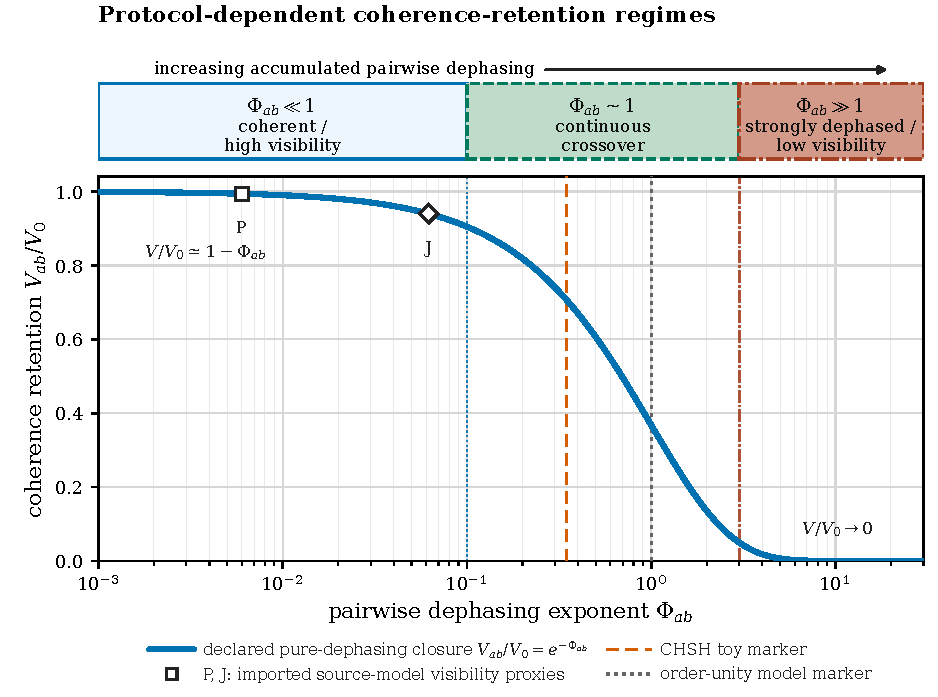
\includegraphics[width=\textwidth]{figures/r153/fig_coherence_regimes_r153.pdf}
\caption{Protocol-dependent coherence retention in the declared
pure-dephasing closure.  The solid blue curve is
\(V_{ab}/V_0=\exp(-\Phi_{ab})\).  The three directly labelled bands show the
asymptotic readings \(\Phi_{ab}\ll1\) (coherent/high visibility),
\(\Phi_{ab}\sim1\) (continuous crossover), and \(\Phi_{ab}\gg1\)
(strongly dephased/low visibility).  The guide edges at \(10^{-1}\) and
\(3\) organise the picture only; they are not physical thresholds.  The
open black markers retain the imported source-model visibility proxies and
the vertical lines retain the declared toy/model markers.  Nothing in this
figure defines a universal quantum--classical boundary, collapse or outcome
selection, or an ECT-specific transition scale without the missing
channel/state/kernel owners.}
\label{fig:gamma_crossover}
\end{figure}

\subsection{Environmental decoherence: C$_{60}$ and macromolecules}
\label{sec:results_environmental}

\textit{Status: standard collisional-decoherence source-model anchor; Open
for a distinct ECT rate.  The condensate action has not supplied the physical
record operator, environmental state, differential cross section, or noise
kernel needed for an ECT prediction.}

For dilute residual gas, the source-model collision rate is
\begin{equation}
  \gamma_{\rm coll}
  =n_{\rm gas}\left\langle v_{\rm rel}
    \sigma_{\rm eff}(v_{\rm rel})\right\rangle,
\end{equation}
with visibility additionally controlled by the momentum-transfer
distribution, path separation, molecular form factor, flight time, and
apparatus protocol~\cite{Arndt1999,Hornberger2003}.  A white-noise amplitude
$D_{\rm eff}$ may parameterise a declared Markov source model, but its use
does not turn that model into a rate derived from ECT.

\paragraph{Comparison with observations.}

\begin{longtable}{@{}L{3.0cm}L{2.6cm}L{3.0cm}L{3.1cm}L{2.3cm}@{}}
\caption{C$_{60}$ and macromolecular environmental-decoherence status.}
\label{tab:env_decoherence_comparison}\\
\toprule
Experiment & Observable & Owning result & ECT status & Assessment \\
\midrule
\endfirsthead
\toprule
Experiment & Observable & Owning result & ECT status & Assessment \\
\midrule
\endhead
\bottomrule
\endfoot
C$_{60}$ interferometer~\cite{Arndt1999}
  & Interference visible
  & Observed/source-model regime
  & No distinct ECT rate
  & Source anchor \\
Fein 2019 (25\,000\,amu)
  & Interference visible
  & Environmental source-model regime
  & No distinct ECT rate
  & Source anchor \\
Pedalino 2026 ($\sim172\,$kDa)
  & Quantum--classical test
  & Standard-QM source model
  & No distinct ECT rate
  & Separation scale; tail qualified \\
\end{longtable}

The observed C$_{60}$ interference is an external experimental
anchor~\cite{Arndt1999}.  Its environmental conditions must be quoted only
from an identified primary owner; the previously repeated $10^{-6}$\,Pa
sub-number is therefore not retained.  Agreement with standard collisional
decoherence is not an ECT-specific discriminator.

\subsection{Di\'osi--Penrose benchmark; ECT record channel Open}
\label{sec:results_gravitational}

\textit{Status: external functional plus one declared hard-sphere
orientation point.  The geometry algebra is exact inside the supplied source
model and the number is Level~C externally; ECT has not derived the required
physical vertex, state-dependent noise kernel, or absolute normalisation.}

The primitive external D--P input is
$\tau_{\rm DP}^{\rm ext}=\hbar/E_G$, with $E_G$ defined by the
mass-density functional in Eq.~\eqref{eq:E_G_DP}.  The idealised point
$C_{\rm DP}(1)=51/160$, $\tau_{\rm DP}^{\rm ext}=70.6\,\mathrm{ms}$ is fixed
by Eqs.~\eqref{eq:dp_hard_sphere_orientation}--
\eqref{eq:dp_hard_sphere_numeric_orientation}; it is neither an uncertainty
statement nor a prediction that ECT decoherence persists in vacuum.  A future
ECT-specific test requires a derived kernel and a held-out feature not shared
by the external functional.

\subsection{External collisional--Di\'osi--Penrose equality scale}
\label{sec:results_crossover}

\textit{Status: exact algebra inside the explicitly supplied hard-sphere and
unit-coefficient external comparison; Level~C as a source-model benchmark;
Open as an ECT result.}

Two different mass constructions must not be conflated.  Inverting an
external D--P time at fixed radius defines the guide mass
$m_{\rm guide}^{\rm DP}$ in Section~\ref{sec:gie_regime_guidance}; it is not a
collisional crossover.  By contrast, take a homogeneous sphere
$m=4\pi\rho R^3/3$, the declared hard-sphere collision rate
$\lambda_{\rm coll}^{\rm hs}=n_{\rm gas}v_{\rm th}\pi R^2$, and the separately
supplied unit-coefficient external comparison
$\lambda_{\rm DP}^{\rm ext}=G_Nm^2/(\hbar R)$.  Equality of those two imported
rates gives
\begin{equation}
 R_{\rm cross}^{\rm coll-DP}
 \sim\left(
 \frac{9\hbar n_{\rm gas}v_{\rm th}}
      {16\pi G_N\rho^2}
 \right)^{1/3},
 \qquad
 m_{\rm cross}^{\rm coll-DP}
 \sim \frac{3\hbar n_{\rm gas}v_{\rm th}}{4G_N\rho}.
 \label{eq:m_cross_results_bench}
\end{equation}
This follows algebraically and dimensionally from the displayed approximate
rate laws.  It is not universal: a different mass-density geometry, branch
separation or D--P regularisation can change the gravitational coefficient
and, outside the displayed unit-coefficient regime, the functional
dependence; a differential cross section, molecular form factor or
momentum-transfer kernel can likewise change the collisional rate law.  No
numerical value is published because the apparatus inputs are not fixed.  Even
after they are fixed, Eq.~\eqref{eq:m_cross_results_bench} compares two external source
models; it is not an ECT crossover or a claim that an ECT channel dominates
or persists in vacuum without the missing vertex, state and noise
normalisation.

% ------------------------------------------------------------------

\subsection{Photonic visibility bounds}
\label{sec:results_photonic}

\textit{Status: source-model/visibility consistency only.}
For a specified pure-dephasing description, a measured visibility defines
$\Phi^{(\rm exp)}=-\ln V$.  The Procopio value is therefore a small
visibility-loss proxy, not a microscopic ECT noise calculation.  Delayed
choice, eraser, swapping, and quantum-switch experiments retain their standard
operational predictions.  No inference that free photons inhabit a different
metric-signature regime, or that detection is a literal signature transition,
follows from these visibilities.

\subsection{Cavity-cat decoherence: next quantitative target}
\label{sec:results_cavity_cat}

\textit{Status: standard cavity-QED source-model target / ECT Open.
The calculation below uses a declared Gaussian--Markov environmental model
with parameters matched to the apparatus.  No distinct environmental or
gravitational ECT rate is derived; the physical vertices, state, noise
kernel, and absolute normalisation remain Open.}

The Haroche--Raimond cavity-QED experiments~\cite{Haroche1993} directly
measure decoherence of mesoscopic microwave-field cat states.  With
$D_{\rm eff}$ matched to the measured cavity lifetime, the declared Markov
closure reproduces the standard cavity-QED scaling.  This is a source-model
consistency check, not evidence that a condensate-gravitational term is
negligible.  A distinct ECT contribution cannot be calculated until its
vertex/state/noise chain is supplied.

% ------------------------------------------------------------------
\subsection{Summary of anchors, proxies, benchmarks, and Open targets}
\label{sec:results_summary}

Table~\ref{tab:decoherence_results_summary} collects the
quantitative estimates, source-model transforms, imported benchmarks, and
Open targets relevant to a future ECT record channel.

\begin{longtable}{@{}L{3.3cm}L{3.6cm}L{3.1cm}L{4.5cm}@{}}
\caption{Summary of source-model estimates, operational proxies, imported
benchmarks, and Open targets relevant to a future ECT record channel.  No row
is an ECT-specific held-out prediction.}
\label{tab:decoherence_results_summary}\\
\toprule
System & Estimate / benchmark & Observation & Status \\
\midrule
\endfirsthead
\toprule
System & Estimate / benchmark & Obs. & Status \\
\midrule
\endhead
\bottomrule
\endfoot
C$_{60}$~\cite{Arndt1999} & Observed interference & Interference \checkmark & External source anchor; pressure sub-number unowned; ECT rate Open \\
Fein 25\,000\,amu & Standard environmental regime & Interference \checkmark & External source anchor; ECT rate Open \\
Pedalino $\sim172$\,kDa & Standard-QM/source-model regime & Quantum/classical separation & Demonstrated separation scale; higher-mass fringe tail not assigned the same status; ECT rate Open \\
Procopio switch & $V=0.994\pm0.002 \Rightarrow \Phi_{\rm vis}=0.006\pm0.002$ & ICO visible & Source visibility transform; ECT kernel Open \\
Di\'osi--Penrose functional & $\tau_{\rm DP}^{\rm ext}=\hbar/E_G$;
$C_{\rm DP}(1)=51/160$, $70.6\,\mathrm{ms}$ at the declared sharp-sphere point &
External formula plus scoped Level-C orientation point & ECT source
projector, vertex, state, noise kernel and normalisation Open; not a data test
or ECT rate \\
Environmental--D--P comparison & Eq.~\eqref{eq:m_cross_results_bench} under
the stated hard-sphere/unit-coefficient assumptions & External conditional
algebra; no numerical value & Not an ECT crossover; ECT channel Open \\
Cavity cat & Open target within present closure
  & Measured decoherence times (Brune 1996)
  & Programme-level target \\
\end{longtable}


% ==============================================================
\section{ECT reduced-state programme for the hybrid-consistency problem}
\label{sec:ect_hybrid_consistency}
% ==============================================================

\textit{Status: structural framing for the gravitational,
measurement, and black-hole sectors of Part~III. No new derivations;
this section fixes the two-level ontology invoked in
Sections~\ref{sec:pes_diosi}, \ref{sec:crooks_ect},
\ref{sec:pes_measurement}, \ref{sec:qs_black_holes}, and the
conditional named-completion tests of
Section~\ref{sec:qs_falsifiers}. The comparison with
theories of Lorentzian emergence (Einstein--aether, Ho\v{r}ava--Lifshitz,
CDT, Hartle--Hawking) given in Section~\ref{sec:comparison_theories}
compares ECT along the signature-emergence axis; the present section
instead compares architectures for the gravity--matter interface. The
two comparison axes are logically distinct.}

\subsection{The hybrid-consistency problem}
\label{sec:hybrid_consistency_problem}

Reconciling a quantum description of matter with a classical or
emergent description of the gravitational sector produces a
characteristic set of structural obstructions known collectively as
the hybrid-consistency problem. Any non-metric-fundamental approach
to the gravity--matter interface must confront at least five
demands:
positivity of reduced states; operational no-signalling;
controlled energy--momentum bookkeeping; relativistic compatibility;
and gauge or diffeomorphism consistency of the emergent mediator.
Historical semi-classical proposals of M{\o}ller and
Rosenfeld~\cite{Moller1962,Rosenfeld1963} already exhibited the
relevant tensions. These were later sharpened by the Page--Geilker
experiment~\cite{PageGeilker_1981} and by a broader literature of
thought experiments and consistency critiques, including the
influential but debated analysis of Eppley and
Hannah~\cite{EppleyHannah_1977}. Low-energy effective-field-theory
treatments~\cite{Donoghue_1994,Burgess_2004} remain internally
consistent in their domain, but do not by themselves resolve the
ultraviolet side or the hybrid measurement problem. The post-quantum classical gravity
programme of
Oppenheim~\cite{Oppenheim_2023_PRX,Oppenheim_etal_2023_NatComm,Grudka_Morris_Oppenheim_2024,Oppenheim_WellerDavies_2023_covariant}
addresses the problem by postulating fundamentally stochastic
dynamics for both metric and matter, at the cost of irreducible
irreversibility and fundamental information loss.

The architectural claim of ECT is not that the five consistency
demands disappear, but that they are displaced from the fundamental
law to the reduction map between the full condensate theory and its
effective descriptions.

\subsection{Central thesis}
\label{sec:central_thesis}

\begin{quote}
\textbf{Conditional programme.} ECT asks whether irreversibility,
decoherence, effective thermality and apparent stochasticity can be realised
as reduced descriptions of a future globally unitary
Euclidean-condensate completion.  This is a research programme, not a
resolution: global unitarity, the physical reduction map, the gravitational
mediator/channel and their joint consistency remain Open.
\end{quote}

The conditional thesis has three components. First, global unitarity
must be established at the level of the full theory. Second, every apparent
cost of hybrid consistency enters only through the reduction to
effective descriptions. Third, the reduction is not a collapse
postulate and not an added stochastic law; it is the choice of which
condensate degrees of freedom are tracked explicitly and which are
integrated out.

Two qualifications are important at the outset. \emph{First}, ECT
does not identify ``non-fundamental metric'' with ``non-quantum
gravity''; what is denied is the need to quantise an independent
metric field as the fundamental starting point. \emph{Second}, in
ECT classicality is not a separate ontological sector but a regime
of reduced description.


\subsection{Full and reduced descriptions: status guard}
\label{sec:two_level_ontology}

The full condensate description and a chosen reduced description must be kept
distinct.  Standard global unitary dynamics is established only in supplied
subsectors for which the complete applicable corrected OS-II package and
reconstruction are in place; reflection positivity alone is insufficient, and
this is not yet a theorem of the full interacting ECT functional.  A reduced
channel may preserve coherence or form
records depending on its physical vertices, state, and protocol.  A small or
large dephasing proxy does not define an ontological phase, quantise gravity,
or decide whether a mediator can entangle.  The useful content of the
Level~IIa/IIb language is therefore operational and conditional, not a
universal $\Gamma_{\rm loop}$ partition.


\paragraph{Level~I --- full condensate description.}

Level~I is the full constrained condensate description before a
resolved/unresolved split.  Its physical observable algebra and state are the
inputs from which any reduction must be derived.

\paragraph{Level~IIa --- reduced coherent-effective description.}

Level~IIa is a coherent effective description after controlled
mode reduction.  Interference remains in the retained sector and no classical
outcome is assumed.

\paragraph{Level~IIb --- reduced macroscopic classical-looking description.}

Level~IIb is a reduced macroscopic description with robust records
for a declared channel.  Approximate diagonality is not ontological outcome
selection.

\paragraph{Bridge between levels.}

A bridge between levels requires an explicit trace/coarse
graining, record operator, state, and error estimate.  The levels must not be
identified by prose alone.  Figure~\ref{fig:two_level_ontology} displays the
resulting status-separated map.
\begin{figure}[htbp]
\centering
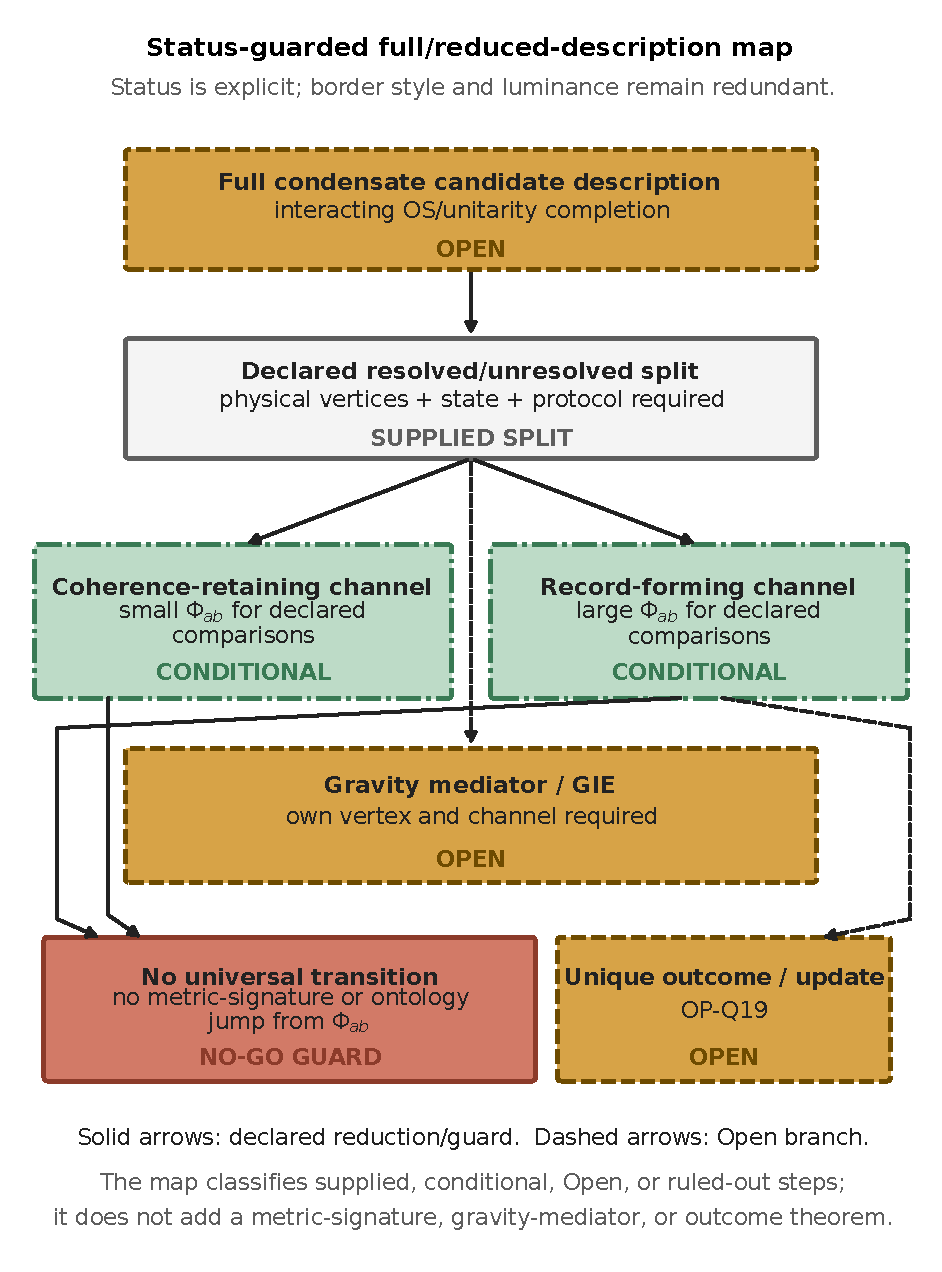
\includegraphics[width=\textwidth]{figures/r155/fig_two_level_ontology_r155.pdf}
\caption{Status-guarded full/reduced-description map.  The declared split can
produce conditional coherence-retaining or record-forming reduced channels;
the gravity-mediator and unique-outcome branches remain Open.  The red node is
the explicit no-go guard that a pairwise record exponent alone causes no
universal metric-signature or ontology transition.  Solid/dashed edges and
literal status words carry the logic independently of colour.}
\label{fig:two_level_ontology}
\end{figure}

\subsection{Costs of consistency across frameworks}
\label{sec:costs_of_consistency}

Each candidate architecture for the gravity--matter interface pays a
characteristic price for consistency. Table~\ref{tab:hybrid_costs}
summarises the main frameworks along four axes: the fundamental
mediator picture, whether fundamental stochasticity or
irreversibility is postulated, whether global unitarity is
maintained at the full-theory level, and the principal consistency
cost.

\renewcommand{\arraystretch}{1.3}
\begingroup
\setlength{\tabcolsep}{5.69pt}
\begin{longtable}{@{}L{3.4cm}L{3.2cm}L{2.5cm}L{2.0cm}L{3.3cm}@{}}
\caption{Costs of consistency for gravity--matter architectures.
The entries are qualitative structural summaries; detailed
references are given in the surrounding text.}
\label{tab:hybrid_costs}\\
\toprule
Framework & Fundamental mediator picture & Fundamental stochasticity / irreversibility & Global unitarity & Main consistency cost \\
\midrule
\endfirsthead
\toprule
Framework & Fundamental mediator picture & Fundamental stochasticity / irreversibility & Global unitarity & Main consistency cost \\
\midrule
\endhead
\bottomrule
\endfoot
Linearised quantum gravity / graviton EFT
 & Quantised gravitational mediator
 & No / No
 & Yes
 & Quantised metric sector; UV non-renormalisability \\
Semi-classical M{\o}ller--Rosenfeld
 & Classical expectation-value geometry
 & No / No
 & Problematic in superposition regimes
 & Hybrid inconsistency tensions (Eppley--Hannah, Page--Geilker) \\
Newton--Schr\"{o}dinger class
 & Classical self-potential in non-linear QM
 & No / No
 & Modified
 & Non-linearity of QM; in the standard additive two-body form, no mediator-based entanglement generation \\
PCCG / Oppenheim
 & Classical metric with fundamental stochastic law
 & Yes / Yes
 & No
 & Fundamental stochasticity and information loss \\
Measurement-feedback hybrids
 & Monitored classical channel
 & Yes / Yes
 & No
 & Explicit monitoring/feedback architecture \\
Phenomenological Di\'{o}si--Penrose collapse
 & Correlated classical noise / collapse law
 & Yes / Yes
 & No
 & Free collapse scale $R_0$; experimental constraints \\
ECT (this work)
 & Candidate reduced mediator programme; no physical mediator has yet been
   derived from the condensate
 & Open; neither fundamental stochasticity nor fundamental irreversibility
   is established or excluded by the present completion
 & Open
 & A future full theory must derive the mediator, reduced channel and
   consistency properties without assuming them \\
\end{longtable}
\endgroup

Read column-by-column, every candidate pays somewhere.  The present ECT
programme places a corresponding burden on a proposed ordered-medium
architecture: a successful completion would have to derive, rather than
presuppose, the physical mediator, the system/environment split, the reduced
channel and any resulting irreversibility, decoherence, effective thermality
or classical-looking gravity.  None of those global properties follows from
the current Level~I${\to}$Level~II bookkeeping alone.  Whether this
architectural choice succeeds
depends on the open items in the status map.  The discriminants in
Section~\ref{sec:qs_falsifiers} become exclusion tests only for a future
named completion that has first fixed the corresponding assumptions.

\subsection{Bridges to the rest of Part~III}
\label{sec:hybrid_bridges}

\paragraph{To the Di\'osi--Penrose benchmark.}
The Di\'osi--Penrose timescale~\cite{Diosi1987,Penrose1996} is used here as an
external phenomenological benchmark, not as a structurally determined
reduced-state limit of condensate distinguishability.  The current ECT action
does not fix it through $\xi_{\rm cond}$ and does not provide the required
state/noise kernel.  Any future comparison with X-ray or levitated-
optomechanics bounds must begin from a declared ECT spectrum and density-
resolution convention.

\paragraph{To the black-hole sector.}
One candidate architecture would extend the reduced-state programme to the
strong-field sector.  Whether reduced thermality or Page-curve-type behaviour
arises from Level~I${\to}$Level~II reduction, from a different completion, or
not at all is Open~(Section~\ref{sec:qs_black_holes}).

\paragraph{To conditional completion tests.}
Section~\ref{sec:qs_falsifiers} records how future observations could exclude
named completions after they have committed to exclusively reduced-state
stochasticity, exact global unitarity or a specific mediator protocol.  These
tests do not turn those presently Open commitments into properties of P1--P6.

\subsection{Scope and non-claims}
\label{sec:hybrid_non_claims}

The present section does not claim:
(i) a closed-form completion of the full non-linear Level~I
dynamics;
(ii) a microscopic derivation of the Level~I${\to}$Level~II
reduction for arbitrary coarse-grainings;
(iii) a strong Level-A prediction of BMV-type gravity-induced
entanglement;
(iv) a complete solution of the single-outcome measurement problem
or an explicit Page-curve derivation from first principles.
Its claim is narrower: ECT provides a single ontological
architecture within which these programmes are jointly well-posed
and can be assessed by common structural criteria.

\paragraph{Forward connection.}
The next section introduces the Principle of Euclidean Stationarity
as one concrete organising principle through which the
Level~I${\to}$Level~II transition becomes physically legible in the
quantum, decoherence, and persistence sectors.

% ==============================================================
\section{Principle of Euclidean Stationarity}
\label{sec:pes}
% ==============================================================


\textit{Status: Level~B as a response--persistence organising framework.
For a declared ECT sector, admissible configurations are supplied by its
causal retarded dynamics, Hamiltonian, Liouvillian, or Floquet problem and are
then classified by physical widths, finite-time retention, and pairwise
record exponents for a declared protocol.  Compact phase and winding
constraints apply only where the sector has that topology.  The ECT-specific
record operators, environment split, retarded/noise kernels, and any unique
outcome rule remain Open (OP-PES-1/OP-Q19; physical record-channel owner).
PES-R does not derive all
quantisation, spectra, least action, or Born weights.}


\medskip
The preceding chapters supply several logically distinct inputs: sector
dynamics and boundary data, the structural action scale in the sectors where
it has been established, and reduced-state influence-functional tools for
declared open systems.  PES-R does not derive or merge those inputs into one
variational law.  It provides a status-separated classification of modes that
have already passed their owning dynamical problem: dynamical admissibility,
finite-time retention, and pairwise record distinguishability are tested separately
(Fig.~\ref{fig:pes_diagram}).  Compact phase and winding are additional
constraints only in sectors that possess that topology.

\begin{figure}[tbp]
\centering
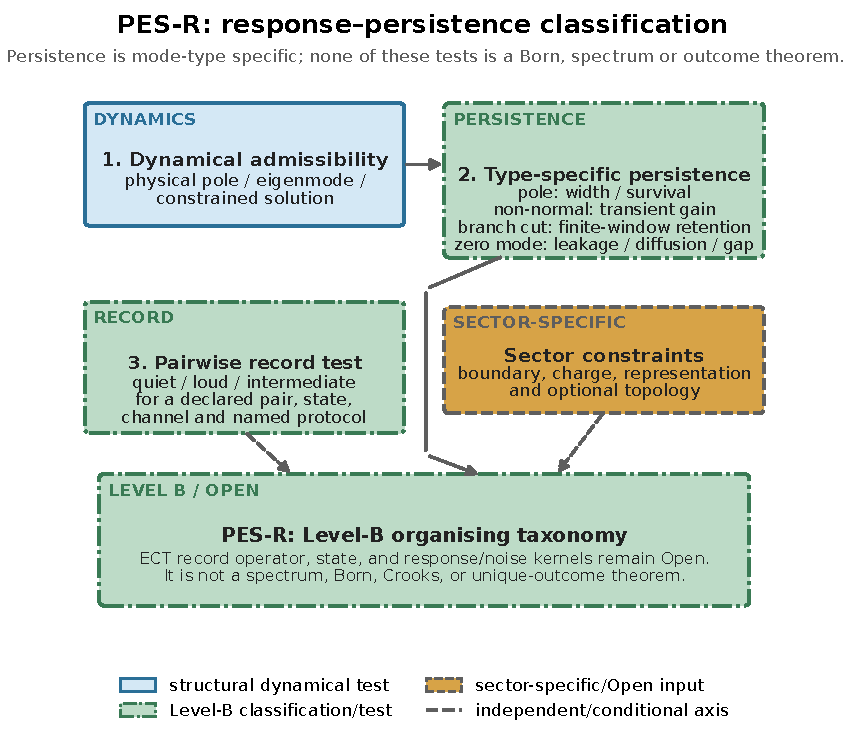
\includegraphics[width=\textwidth]{figures/r155/fig_pes_diagram_r155.pdf}

\caption{Response--persistence formulation of PES-R.  A candidate must be
dynamically admissible and receive a pairwise record classification for a
named state, channel and protocol.  Persistence is tested by a criterion
appropriate to the spectral object: width/survival for an isolated pole,
transient gain or finite-time singular values for non-normal dynamics,
finite-window retention for a branch cut, and leakage, diffusion or a gap
for a zero mode.  Boundary, charge, representation and optional topology
remain sector-specific constraints.  PES-R is a Level-B organising
taxonomy, not a spectrum, Born, Crooks or unique-outcome theorem; its ECT
record operator, state and response/noise kernels remain Open.}

\label{fig:pes_diagram}
\end{figure}

% ------------------------------------------------------------------
\subsection{Statement of the principle}
\label{sec:pes_statement}


\paragraph{Short formulation.}
\begin{quote}
\textbf{Principle of Euclidean Stationarity, response--persistence form
(PES-R).}
\emph{Within a declared ECT sector, first solve the physical causal or
constrained dynamical problem.  Then classify the resulting modes by their
finite-time retention and pairwise record distinguishability, subject to the
sector's boundary, charge, representation, and---where present---topological
constraints.  PES-R classifies finite-window persistence using preregistered
diagnostics appropriate to the spectral type; it supplies no universal scalar
or cross-type ranking.  It does not generate every spectrum, derive Born
weights, or select a unique outcome.}
\end{quote}


\paragraph{Why this is not a new postulate.}

PES-R is not a new fundamental postulate and is not a universal
variational law.  It is a status taxonomy assembled from separately owned
dynamics, retention, and record calculations.

\paragraph{Derivational status.}
PES-R assembles three distinct structures already used in the manuscript:
(i) the sector's causal or constrained dynamics; (ii) its spectral and
boundary data; and (iii) a pairwise influence-functional record exponent for
a declared resolved/unresolved split.  The tolerances and observation window
are protocol data.  The ECT-specific split, record operators, kernels, and a
universal one-history path measure have not been derived and remain
OP-PES-1 physical-channel inputs.

\medskip\noindent\textbf{PES-R/static-response firewall.}
PES-R does not derive S11, ERP binary recruitment, the minimum-energy
continuation, HRC-0/HRC-3, or the gravity bridge.  Conversely, the HRC static
primitive does not supply the retarded/noise kernels or record operators
needed by PES-R.  Any common scalar/orientation modes require one
resolved/unresolved split, canonical normalisation, and an explicit
subtraction ledger.  A finite readout coupling may shift a constitutive
threshold; the protected-probe limit, a Ward identity, a counterterm, or the
shifted law must therefore be stated rather than assumed.  This paragraph is
a no-conflict/double-counting guard, not a derivation of either framework.

\medskip\noindent\textbf{Notation firewall: occupation versus noise.}
The HRC recruitment/occupation variable is reserved as $\mathcal Q$.
The symbols $N(t-t')$ and $N^{(S)}(\omega)$ are reserved exclusively for the
PES-R time-domain and spectral noise kernels, with
$S_H(\omega)=S_0N^{(S)}(\omega)$.  No $N$ appearing in the PES-R sector is an
HRC occupation number, and no $\mathcal Q$ appearing in the HRC sector is a
noise kernel.

\subsection{Formal realisation}
\label{sec:pes_formal}


\paragraph{Two-history influence functional and causal response.}
Let $q_c=(q_++q_-)/2$ and $q_\Delta=q_+-q_-$:
\begin{equation}
  q_c=\frac{q_++q_-}{2},\qquad q_\Delta=q_+-q_- .
  \label{eq:pes_keldysh_variables}
\end{equation}
Fix a joint initial preparation at $t_0$ and a closed-time-path contour, and
centre the unresolved-sector one-point functions or absorb their contribution
into $S_{\rm sys}$.  For a Gaussian unresolved sector coupled through
physical record operators $\mathcal O_a[q]$, the bulk coarse-grained
effective action has the schematic Feynman--Vernon/Schwinger--Keldysh form
\cite{FeynmanVernon1963,CaldeiraLeggett1983}:
\begin{align}
 S_{\rm bulk}={}&S_{\rm sys}[q_+]-S_{\rm sys}[q_-]
 +\int dX\,dX'\,\Delta\mathcal O_a(X)D^R_{ab}(X,X')
 (\mathcal O_b)_c(X') \\
 &+\frac{i}{2}\int dX\,dX'\,\Delta\mathcal O_a(X)N_{ab}(X,X')
 \Delta\mathcal O_b(X'),
 \label{eq:pes_cgea}
\end{align}
where $D^R$ is causal and $N=N^\dagger\succeq0$.  A compatible factorised
preparation is sufficient for this bulk form without an additional
initial-correlation influence term.  For a correlated preparation the full
effective action is instead
\begin{equation}
 S_{\rm CGEA}^{\rm corr}[q_+,q_-]
 =S_{\rm bulk}[q_+,q_-]+S_{\rm ic}[q_+,q_-;t_0],
 \label{eq:pes_cgea_initial_correlations}
\end{equation}
or is represented equivalently on an extended contour.  The term
$S_{\rm ic}$ may be omitted only after it has been shown to vanish or to have
been absorbed consistently.  The non-negative bulk pairwise record exponent
is
\begin{equation}
  \Phi_{\rm dec}^{\rm bulk}[q_+,q_-]
  =\frac{1}{2S_0}\int dX\,dX'\,
  \Delta\mathcal O_a(X)N_{ab}(X,X')\Delta\mathcal O_b(X')\ge0 .
  \label{eq:Phi_dec_general}
\end{equation}
The full log-modulus diagnostic $\Xi_{ab}^{\rm full}=-\ln|\mathcal F|$ may
additionally contain preparation-dependent initial-boundary terms and need
not be nonnegative without a contractivity premise.

\paragraph{Distinction: stationarity, disturbance, action.}

Stationarity of the system action, small physical decay width, and
small pairwise record exponent are inequivalent.  Each has its own units,
kernel, and experimental owner.

\medskip\noindent\textbf{Normalisation dictionary: $N$, $S_H$, and the finite record.}
The full log-modulus diagnostic is defined operationally before any kernel
convention,
\begin{equation}
  \Xi_{ab}^{\rm full}(T):=-\ln|\mathcal F[a,b;T]|,
  \qquad
  \Phi_{ab}(T):=\Xi_{ab}^{\rm full}(T)\geq0
  \quad\text{only when }|\mathcal F[a,b;T]|\leq1
  \text{ has been established}.
  \label{eq:pes_Phi_operational}
\end{equation}
After the spatial/projector integrations have produced a finite vector of
record differences $\Delta\mathcal O_{ab}(t)$, assume only for this spectral
rewrite that the bulk state and noise kernel are stationary on the observation
window, so that $N(t,t')=N(t-t')$, and that initial-boundary/preparation
transients are absent, negligible on that window, or explicitly separated.
Without these premises the two-time kernel $N(t,t')$ must be retained and no
single-frequency kernel $N^{(S)}(\omega)$ is defined generically.  Under the
stated premises we use the unnormalised finite-window and Fourier conventions
\begin{align}
 d_{ab,T}(\omega)&:=\int_0^Tdt\,e^{i\omega t}
                   \Delta\mathcal O_{ab}(t),\\
 N^{(S)}(\omega):=\widetilde N(\omega)&:=\int_{-\infty}^{\infty}d\tau\,
                   e^{i\omega\tau}N(\tau),
 \qquad
 N(\tau)=\int_{-\infty}^{\infty}\frac{d\omega}{2\pi}
                   e^{-i\omega\tau}N^{(S)}(\omega).
 \label{eq:pes_fourier_dictionary}
\end{align}
The action-scaled spectral record kernel used in the PES-R robustness
statements is, by definition,
\begin{equation}
  S_H(\omega):=S_0\,N^{(S)}(\omega),
  \qquad S_H(\omega)=S_H^\dagger(\omega)\succeq0 .
  \label{eq:pes_SH_dictionary}
\end{equation}
The time-domain and spectral expressions are then the same bulk contribution:
\begin{equation}
\boxed{
  \Phi_{ab}^{\rm bulk}(T)
  =\frac{1}{2S_0}\int_0^Tdt\int_0^Tdt'\,
       \Delta\mathcal O_{ab}^\dagger(t)N(t-t')
       \Delta\mathcal O_{ab}(t')
  =\frac{1}{2S_0^2}\int_{-\infty}^{\infty}\frac{d\omega}{2\pi}\,
       d_{ab,T}^\dagger(\omega)S_H(\omega)d_{ab,T}(\omega) .}
  \label{eq:pes_Phi_dictionary}
\end{equation}
If $S_{\rm ic}$ is absent or has no modulus contribution on the declared
protocol, then
$\Xi_{ab}^{\rm full}=\Phi_{ab}=\Phi_{ab}^{\rm bulk}\geq0$.  Otherwise
$\Xi_{ab}^{\rm full}$ also contains the explicitly retained preparation term
and cannot be reconstructed from $N(t-t')$ alone; a nonnegative full
$\Phi_{ab}$ is \textsc{not identifiable} until full contractivity is proved.
Thus the time quadratic has units $[S_0]$, the spectral integral has units
$[S_0]^2$, and both displayed ratios are dimensionless.  No factor of $T$ is
hidden in $d_{ab,T}$; a periodogram convention divided by $T$ would require
the compensating factor in its spectral kernel.  $S_H$ is an action-scaled
record spectrum for the declared operator normalisation, not an independently
identified raw detector covariance.  $D^R$ remains a distinct causal response
kernel: stationarity, positivity, or an equilibrium fluctuation--dissipation
relation does not identify response and noise without the required state and
KMS assumptions.
The mean equation follows by varying the complete coarse-grained action and
taking the physical diagonal,
\begin{equation}
 \left.
 \frac{\delta\!\left(S_{\rm bulk}+S_{\rm ic}\right)}
      {\delta q_\Delta(X)}
 \right|_{q_\Delta=0}=0,
 \qquad S_{\rm ic}=0\ \text{when no such term is present},
 \label{eq:pes_retarded_mean}
\end{equation}
with the retarded force and nonlinear vertices understood.  The first
derivative of the bulk noise quadratic is proportional to $Nq_\Delta$ and
vanishes on the diagonal.  Noise therefore controls bulk fluctuations and
branch records rather than supplying a generic additional mean potential.
A correlated-preparation term $S_{\rm ic}$ can nevertheless contribute to
the mean equation and must be varied rather than silently discarded.

\paragraph{Translation susceptibility: optional diagnostic.}
For a declared deformation
$q_\varepsilon=q+\varepsilon\eta+O(\varepsilon^2)$, keep the state, kernel,
record protocol and interval fixed.  A finite bulk susceptibility follows
only if the record map is differentiable in the quadratic-form topology of
$N$:
\begin{equation}
 \Delta\mathcal O[q,q_\varepsilon]
 =-\varepsilon\,D\mathcal O_q[\eta]+r_\varepsilon,
 \qquad
 D\mathcal O_q[\eta]\in\operatorname{Dom}(N^{1/2}),
 \qquad
 \|N^{1/2}r_\varepsilon\|=o(|\varepsilon|).
 \label{eq:Gamma_tr_form_domain}
\end{equation}
Under these premises,
\begin{equation}
 \Gamma_{\rm tr}^{\rm bulk}[q;\eta]
 :=\lim_{\varepsilon\to0}
   \frac{\Phi_{\rm dec}^{\rm bulk}[q,q_\varepsilon]}{\varepsilon^2}
 =\frac{1}{2S_0}
   \bigl\|N^{1/2}D\mathcal O_q[\eta]\bigr\|^2
 \ge0 .
 \label{eq:Gamma_tr_def}
\end{equation}
If form-domain differentiability or finiteness has not been established, the
only generally defined diagnostics are the extended quantities
\begin{equation}
 \underline{\Gamma}_{\rm tr}^{\rm bulk}
 :=\liminf_{\varepsilon\to0}
   \frac{\Phi_{\rm dec}^{\rm bulk}[q,q_\varepsilon]}{\varepsilon^2},
 \qquad
 \overline{\Gamma}_{\rm tr}^{\rm bulk}
 :=\limsup_{\varepsilon\to0}
   \frac{\Phi_{\rm dec}^{\rm bulk}[q,q_\varepsilon]}{\varepsilon^2},
 \qquad
 \underline{\Gamma}_{\rm tr}^{\rm bulk},
 \overline{\Gamma}_{\rm tr}^{\rm bulk}\in[0,\infty].
 \label{eq:Gamma_tr_extended}
\end{equation}
A finite $\Gamma_{\rm tr}$ exists only when these two quantities coincide
and are finite; otherwise the finite susceptibility is reported as
\textsc{not identifiable}, rather than assumed.  With a correlated initial
preparation, $S_{\rm ic}$ may also contribute to the full
$-\ln|\mathcal F|$ and hence to a full translation susceptibility; the bulk
formula above is not by itself that full result.

Its value depends on the direction normalisation, state, record operators,
interval, and boundary prescription.  Within one fixed choice of all those
data it may order already admissible modes; it supplies no cross-protocol or
cross-type ranking, but varying it together with the system action would
introduce a force not derived from the influence functional.  A one-history
Onsager--Machlup route requires a separately derived path measure, drift,
diffusion, Jacobian, stochastic convention, and boundary data; that route is
Open.


\paragraph{Relation to extremal action.}
Closed-sector constrained extrema remain the starting point.  In an open
sector the retarded kernel shifts poles and widths, while the noise kernel
governs pairwise records.  PES-R therefore does not replace the closed-sector
variational equation by an additive one-history noise-gradient equation.

\paragraph{Retention set and separate pairwise record classification.}
For a declared sector $\mathcal C_n$, observation window $T$, and tolerances,
define the protocol-level retention set
\begin{equation}
  \mathfrak P^{\rm ret}_{\boldsymbol\varepsilon}(T)
  =\bigcup_n\left\{a\in\mathcal C_n:\begin{array}{l}
  a\text{ solves the declared physical response/spectral problem},\\
  \text{the retention diagnostics applicable to its spectral type}\\
  \text{meet the preregistered finite-window tolerances},\\
  \text{sector boundary, charge, representation, and optional topology hold}
  \end{array}\right\}.
  \label{eq:persistent_sector}
\end{equation}
The relevant diagnostic set is type-dependent rather than one universal
conjunction: an isolated pole uses its physical width and survival/residue; a
non-normal or Jordan sector uses the singular-value gain in a declared norm
together with full finite-window retention; a cut-dominated object uses the
finite-window survival functional directly; and a zero mode uses leakage,
diffusion, or gap diagnostics rather than a quality factor.  At an exceptional
point the defective Jordan block, not ill-defined coalescing residue labels,
is the object to classify.  All objects are defined after gauge/constraint
reduction.

For a channel in which a nonnegative full $\Phi_{ab}$ has been established,
the pairwise record exponent is an independent axis, not a property of one
mode and not a necessary retention condition.  With preregistered thresholds
$\varepsilon_{\rm quiet}<\varepsilon_{\rm loud}$, define
\begin{align}
 \mathcal Q_\Phi(T)&:=\{(a,b):\Phi_{ab}(T)\le
 \varepsilon_{\rm quiet}\},\\
 \mathcal L_\Phi(T)&:=\{(a,b):\Phi_{ab}(T)\ge
 \varepsilon_{\rm loud}\}.
 \label{eq:pes_record_quiet_loud}
\end{align}
Pairs between the thresholds are intermediate.  Small $\Phi_{ab}$ means that
the owning channel is record-quiet and the compared coherence can persist or
revive; large $\Phi_{ab}$ means strong pairwise dephasing and suppression of
the corresponding off-diagonal element in the named reduced channel.  Calling
that suppression an accessible physical record additionally requires an
identified environmental or readout observable.  Objective pointer redundancy
is a still stronger, fragment-resolved condition and is not inferred from one
scalar $\Phi_{ab}$.

To combine the two axes without confusing an object with a pair, define
\begin{equation}
 R_{ab}(T):=\mathbf 1\!\left[
 a,b\in\mathfrak P^{\rm ret}_{\boldsymbol\varepsilon}(T)\right].
 \label{eq:pes_pair_retention_flag}
\end{equation}
The joint taxonomy then contains six cells,
$R_{ab}\in\{0,1\}$ times
$\{\text{quiet},\text{intermediate},\text{loud}\}$.  The four
quiet/loud endpoint cells are only the extreme subtable obtained after the
intermediate band has been excluded; retaining zero, one, or two members of
the pair would instead give a finer nine-cell diagnostic.  This is a Level-B
protocol taxonomy, not a necessary-and-sufficient persistence, pointer, or
outcome theorem.

\paragraph{Non-normal, higher-order-pole, and cut guard.}
Let $U_{\rm phys}(t,0)$ be the amplitude propagator after the declared
constraint/gauge reduction, let $P_a=P_a^\ddagger=P_a^2$ be the orthogonal
physical projector onto the block being classified, and let
$\|\cdot\|_{\rm phys}$ be a preregistered positive physical norm.  The block
gain is
\begin{equation}
 \mathcal G_a(T):=
 \sup_{0\le t\le T}\|P_aU_{\rm phys}(t,0)P_a\|_{{\rm phys},\,\rm op} .
 \label{eq:pes_finite_window_gain}
\end{equation}
For density-operator or Liouvillian evolution, let $\mathcal E_t$ be the
declared physical reduced map and let $0\preceq E_a\preceq I$ be a positive
effect representing survival in the declared sector.  For a normalized
initial density operator $\rho_a$ prepared wholly in that sector,
$\operatorname{Tr}_{\rm phys}(E_a\rho_a)=1$, the survival probability is
\begin{equation}
 \mathcal S_a(t;\rho_a):=
 \operatorname{Tr}_{\rm phys}\!\left[E_a\mathcal E_t(\rho_a)\right],
 \qquad 0\le t\le T ,
 \label{eq:pes_finite_window_survival}
\end{equation}
where $\ddagger$ denotes the adjoint in the declared physical inner product.
A non-normal Riesz projector is not silently substituted for the positive
effect in this probability.  If the initial preparation is not wholly in the
sector, the ratio to its initial occupation is merely a normalized retention
ratio and can exceed unity through inflow; it is not called a probability.
The initial state or admissible state class,
projector/effect, norm, observation window, and tolerance functional on the
full curve must be listed by each application; neither equation is a universal
scalar selection rule.  For
non-normal physical evolution the finite-time singular values of the reduced
propagator, not the eigenvalue real parts alone, control transient gain.  A
Jordan block or higher-order pole generates polynomial prefactors multiplying
its exponential contribution, while a branch cut can generate an algebraic
long-time tail.  Therefore $\mathcal G_a(T)$ and the full curve
$\mathcal S_a(t;\rho_a)$ must include pole, Jordan and cut contributions over
the declared finite window; a small modal width by itself is insufficient.

\subsection{Immediate consequences}
\label{sec:pes_consequences}


\subsubsection*{Spectral discreteness and persistence}

A discrete spectrum is supplied by the sector operator, its domain, boundary
conditions, and potential---for example by a self-adjoint operator with
compact resolvent.  Such spectra exist on topologically trivial configuration
spaces.  PES-R asks which supplied modes remain persistent; it does not
create the spectrum from compact phase.  Compact phase remains important in
sectors where it adds winding, flux, circulation, holonomy, or charge labels.


\subsubsection*{Extremal action and persistence}

Extremal action and open-system persistence answer different questions.
Constrained extrema determine closed-sector solutions; a retarded environment
shifts poles and widths; the noise kernel controls record distinguishability.
No general bound relating $|\delta S_E|$ to a decoherence exponent has been
derived.  A survival derivation of least action remains OP-PES-2.


\subsubsection*{Stationary, oscillatory, and decoherence-free modes}

Stationarity is spectral rather than the universal coordinate condition
$\partial_w\Psi=0$.  An energy eigenprojector may be stationary while its
state vector acquires phase; resonances have finite width; Liouvillian and
Floquet modes may persist at nonzero frequency.  Environmental silence for a
pair requires the physical record difference to lie in the null space of the
noise kernel.  Widths must be calculated from vertices, retarded
self-energies, form factors, channels, occupation factors, and phase space.


\subsubsection*{Connection to $S_0=\hbar$: no PES-R derivation}

The fixed-core and positive-tension loop constructions assign distinct
sector-specific coefficients $\iota_0^{\rm EFT}$ and
$\iota_{0,\rm bal}^{\rm eff}$, but PES-R selects neither owner map to the
operational $S_0$ and proves no cross-sector universality.  Identifying
$S_0$ with $\hbar$ requires a separate canonical/experimental matching and
remains Level~B/Open.  Persistence provides no
independent upgrade of that status and no universal lower-action theorem.

\subsubsection*{Gravitational sector: conditional programme}

ECT proposes that gravitational and matter excitations belong to one
condensate architecture.  It has not derived that they share one canonical
action quantum, nor has PES-R quantised the physical tensor sector.  Closing
this claim requires the tensor modes, constraints, canonical normalisation,
propagator, interacting RP/OS reconstruction, and comparison of the resulting
action scale with the electromagnetic one.  Cross-sector universality and
``no separate quantisation step'' therefore remain Open hypotheses
(OP-PES-3), not predictions.

\subsection{Relation to known selection mechanisms}
\label{sec:pes_landscape}

PES did not appear in a vacuum: several of its special cases are
classic results, and its quantum-information face has a developed
formalism.  Placing PES in this landscape both anchors it and makes
precise what is new.


\paragraph{Physical analogies, not validations.}
The Landau critical-velocity condition, environment-stabilised molecular
chirality, and measured resonance widths illustrate three different
mechanisms---kinematic channel closure, record-induced dephasing, and retarded
pole decay~\cite{Landau1941,HarrisStodolsky1978}.  PES-R offers a common vocabulary for comparing their retention,
but it does not derive these results or identify them with one scalar
``quietness'' mechanism.  Lifetimes and widths remain owned by their physical
vertices, self-energies, states, and phase space.


\paragraph{Quantum-information anchors.}
Environment-induced superselection, predictability sieves,
decoherence-free subspaces, noiseless subsystems, and quantum Darwinism are
established open-system structures
\cite{Zurek1981,Zurek1982,Zurek2003,ZurekHabibPaz1993,ZanardiRasetti1997,LidarChuangWhaley1998,Zurek2009,WickWightmanWigner1952}.
In matrix notation exact quietness of a
declared record difference $d(\omega)$ requires
$S_H^{1/2}(\omega)d(\omega)=0$ almost everywhere.  Infrared superselection is a pairwise divergence of $\Phi_{ab}$, not a
one-history zero-noise or ``quietness'' condition.

If $S_H(\omega)\sim\omega^a$ and
$|d(\omega)|\sim\omega^{-\sigma}$, the infrared integral scales as
\begin{equation}
  \Phi_{\rm IR}\sim\int_0^\Omega d\omega\,
  \omega^{a-2\sigma-\zeta},\qquad
  \zeta=0\ (T=0),\quad \zeta=1\ (\text{thermal IR tail}),
  \label{eq:pes_ir_superselection}
\end{equation}
and diverges when $a-2\sigma-\zeta\le-1$.

\paragraph{ECT-specific status.}
ECT hypothesises that the unresolved sector belongs to the same condensate,
but the split, record operators, and kernels have not been derived from the
bare action.  PES-R organises possible ECT applications of einselection; it
does not yet derive or extend einselection from first principles.


\subsection{Stability, lifetimes, and decay widths}
\label{sec:pes_lifetimes}

Long-lived excitations are real poles or poles/Liouvillian modes with small
damping.  Their widths are determined by the retarded self-energy,
interaction vertices, form factors, available channels, occupation factors,
and phase space.  A translation susceptibility may be tested as a correlate
of selected form factors, but it is not a universal lifetime law.  The former
ansatz is retained only as an explicitly Open target,
\begin{equation}
  \gamma_a\stackrel{?}{\propto}\Gamma_{\rm tr}[q_a;\eta_a],
  \label{eq:pes_lifetime}
\end{equation}
after OP-PES-4 supplies physical kernels and normalisation.  No observed
particle-lifetime hierarchy is claimed as an ECT prediction at present.


\paragraph{Instability from a residual broadening or decay channel.}

A residual coupling can destabilise a mode only through its self-energy,
phase space, and state.  Pairwise record loudness is a separate property and
is not a universal scalar source of instability.

\paragraph{Qualitative hierarchy.}

Any qualitative lifetime hierarchy remains conditional on the
physical vertices and densities of states.  PES-R can compare computed
widths; it cannot generate them from topology alone.
For audit continuity, representative external lifetime landmarks are retained
as inputs only~\cite{ParticleDataGroup2022,SuperK2020}:
\begin{longtable}{@{}L{3.2cm}L{3.2cm}L{8.2cm}@{}}
\caption{Representative particle-lifetime data.  These values constrain a
future width calculation; they do not validate PES-R or determine
$\Gamma_{\rm tr}$.}
\label{tab:pes_lifetimes}\\
\toprule
Particle & Lifetime / bound & ECT status \\
\midrule
\endfirsthead
\toprule
Particle & Lifetime / bound & ECT status \\
\midrule
\endhead
\bottomrule
\endfoot
Proton & $>10^{34}$\,yr & External lower bound; microscopic ECT stability derivation Open \\
Electron & Stable within observations & External fact; owning symmetry/decay-channel argument required \\
Neutron (free) & $\simeq879$\,s & External input \\
Muon & $\simeq2.2\,\mu$s & External input \\
Charged pion & $\simeq26$\,ns & External input \\
$W$ boson & $\sim3\times10^{-25}$\,s & Width-derived external scale \\
\end{longtable}


\paragraph{Rydberg states: external target only.}

Long Rydberg lifetimes do not test ECT while its electromagnetic and
environmental channels are missing.  They are external data for a future
owner-complete calculation, not a qualitative consistency check.

\subsection{Quality factors, persistent bands, and finite spectra}
\label{sec:pes_quietness}

Distinguish the dimensionless pairwise exponent $\Phi_{ab}(T)$, decay rate
$\gamma_a$, and energy width $\Gamma_{E,a}=S_0\gamma_a$.  For angular
frequency $\Omega_a$ and $E_a=S_0\Omega_a$,
\begin{equation}
  Q_{\omega,a}=\frac{\Omega_a}{\gamma_a}
  =\frac{E_a}{\Gamma_{E,a}},\qquad
  N_{{\rm coh},a}=\frac{Q_{\omega,a}}{2\pi}.
  \label{eq:pes_quietness}
\end{equation}
For the isolated-pole subclass with a declared exponential survival law
$P_a(T)=e^{-\gamma_aT}$, the condition
$P_a(T_{\rm obs})\ge P_{\min}$ gives
$Q_{\omega,a}\ge\Omega_aT_{\rm obs}/[-\ln P_{\min}]$.
Within that subclass a declared high-quality-factor count is
\begin{equation}
  N_{\rm persistent}=\#\{a:Q_{\omega,a}>Q_{\rm sel}\},
  \label{eq:pes_persistent_count}
\end{equation}
with the line-shape and protocol convention declared.  This is a
coherent-cycle/high-$Q$ count, not the general retention set of
Eq.~\eqref{eq:persistent_sector}; when $\Omega_a$ varies, a common
$Q_{\rm sel}$ is not a common finite-window survival threshold.  A common
survival threshold instead uses the mode-dependent bound above, equivalently
$\gamma_a\le-\ln P_{\min}/T_{\rm obs}$.  Branch-cut, non-normal,
exceptional-point and zero-mode objects require their type-specific retention
diagnostics.

In the following positive two-channel toy, the persistent sector can be a
finite \emph{band} rather than a prefix of low-lying modes.  If, for
asymptotic energies $E_n\sim A\,n^{s}$, the
environmental width contains both an infrared-enhanced and an
ultraviolet-enhanced broadening channel on top of the barrier one,
\begin{equation}
  \label{eq:pes_band_width}
  \Gamma_n
  =
  \Gamma_n^{\rm tunnel}
  +\gamma_-\,n^{-r}
  +\gamma_+\,n^{p},
  \qquad r>0,
  \qquad p>s,
\end{equation}
then, in the high-barrier limit,
\begin{equation}
  \label{eq:pes_band_Q}
  Q_n
  \simeq
  \frac{A\,n^{s}}{\gamma_-\,n^{-r}+\gamma_+\,n^{p}},
\end{equation}
the exact high-barrier persistent set is
\begin{equation}
  \label{eq:pes_band_exact_set}
  \mathcal I_Q=\left\{n\in\mathbb N:
  \gamma_-n^{-(s+r)}+\gamma_+n^{p-s}<\frac{A}{Q_{\rm sel}}\right\}.
\end{equation}
For $s+r>0$ and $p>s$, convexity in $\ln n$ makes this set a single
integer interval when it is nonempty.  Its exact real endpoints are roots of
the combined equality, not of the two terms separately.  The separate-term
bounds give only the necessary outer enclosure
\begin{equation}
  \label{eq:pes_band_window}
  \left(\frac{\gamma_-\,Q_{\rm sel}}{A}\right)^{1/(s+r)}
  < n <
  \left(\frac{A}{\gamma_+\,Q_{\rm sel}}\right)^{1/(p-s)}.
\end{equation}
A simple sufficient inner enclosure is obtained by requiring each positive
term to be smaller than $A/(2Q_{\rm sel})$:
\begin{equation}
  \label{eq:pes_band_inner_window}
  \left(\frac{2\gamma_-\,Q_{\rm sel}}{A}\right)^{1/(s+r)}
  < n <
  \left(\frac{A}{2\gamma_+\,Q_{\rm sel}}\right)^{1/(p-s)}.
\end{equation}
The exact count is $N_{\rm persistent}=\#\mathcal I_Q$, with maximal quality
factor at
$n_*^{\,p+r}=(s+r)\,\gamma_-/[(p-s)\,\gamma_+]$.
Thus the positive two-channel toy can produce a finite window --- neither the
softest nor the hardest modes need survive --- but either enclosure may contain
no integer and the exact set may be empty.
This toy parameterisation is not an ECT mass calculation; it only
illustrates the mechanism by which condensate spectral data can
produce a finite persistent sector.
More generally, for $E_n\sim A\,n^{s}$ and multi-channel widths
$\Gamma_n=\sum_i\gamma_i\,n^{b_i}$ the narrow-width condition reads
$\sum_i\gamma_i\,n^{\,b_i-s}<A/Q_{\rm sel}$; a channel with $b_i>s$ enforces
an ultraviolet cap, a sufficiently strong channel with $b_i<s$ removes
the lowest modes, and, since $\sum_i\gamma_i\,e^{(b_i-s)\ln n}$ is
convex in $\ln n$, its sublevel set is one contiguous interval, possibly
empty or unbounded, within this positive monomial asymptotic family.  This
conclusion is not generic for resonant or nonmonotone form factors, which can
produce disjoint windows.  When the ultraviolet channel arises from resonant sampling of a
spectral density $J(\omega)\sim\omega^{a}$ with squared form-factor
scaling $n^{u}$, its exponent is fixed by the dictionary $p=as+u$.
Within this isolated-pole toy family,
Eq.~\eqref{eq:pes_persistent_count} converts the declared high-$Q$ count into
a spectral problem: determine $(E_n,\Gamma_n)$ from
the condensate defect spectrum --- schematically
$\Gamma_n\sim\int_0^\infty d\omega\,J(\omega,\mathbf{x})\,|F_n(\omega)|^{2}$
with $F_n$ the mode form factor --- then count.  It does not determine the
number of generations, create the supplied spectrum, or classify general
non-pole stability.
\emph{Status: Level~B as a mathematical mechanism; the ECT
microphysical input --- the spectral data $(E_n,\Gamma_n)$,
equivalently the condensate spectral density
$J(\omega,\mathbf{x})$ and the mode form factors $F_n$ --- is Open
and constitutes the common target
of OP-PES-1, OP-PES-2, and OP-PES-4.}


\subsection{Sector-specific quantisation and PES-R status}
\label{sec:pes_quant_table}

PES-R does not identify one universal origin of quantisation.  The owning
sector supplies each spectrum or representation; PES-R can only classify
finite-time persistence afterwards.
\begin{longtable}{@{}L{3.2cm}L{3.0cm}L{5.8cm}L{2.5cm}@{}}
\caption{Sector-specific quantisation mechanisms and honest status.}
\label{tab:pes_quantisation}\\
\toprule
Quantity & Owning mechanism & PES-R role & Status \\
\midrule
\endfirsthead
\toprule
Quantity & Owning mechanism & PES-R role & Status \\
\midrule
\endhead
\bottomrule
\endfoot
$S_0=\hbar$ & Empirical calibration of the operational ECT action-unit slot & Calibration explicit; physical owner and absolute derivation Open & B calibration / Open owner \\
Bound-state levels & Hamiltonian/\allowbreak operator, domain, potential, boundaries & Retention after spectrum is solved & A/B \\
Angular momentum / spin & Rotation-group representations and topology & Sector constraints only & A/B \\
Electric charge / flux & Owning compact gauge sector & Sector constraints only & A/B/Open \\
Gravitational quanta & Physical tensor-mode reconstruction & Persistence test after kernel closure & Open \\
Area scale & Strong-field/entropy programme & No derivation from PES-R & Open \\
\end{longtable}


\subsection{Measurement, information, and decoherence: summary}
\label{sec:pes_measurement_summary}

Specified reduced channels can suppress interference and form stable records.
The qubit information--dephasing calculation is a model-specific trade-off,
not a protocol-independent measurement bound.  PES-R supplies no outcome
update rule and no identity between photon proper time, coherence, and
collapse.

% ------------------------------------------------------------------
\subsection{Protocol reversal and tunnelling geometry: summary}
\label{sec:pes_revtun_summary}

Tunnelling retains its stated WKB/instanton and geometric status.  A
reverse/forward fluctuation relation requires explicit path measures and local
detailed balance; no ratio is inferred from the pairwise decoherence exponent.

% ------------------------------------------------------------------
\subsection{Geometric locking conjecture: Open}
\label{sec:pes_alpha_beta}


\paragraph{What happens at $\alpha\to\beta$.}

At $\alpha\to\beta$ the kinetic tensor becomes singular in the
owning signature analysis.  No universal decoherence transition or
quantum--classical boundary follows from that singularity.

\paragraph{Conjectural bridge to decoherence.}

No signature-boundary record channel is defined without an explicit vertex,
state, and constraint-reduced kernel.  A connection between the signature
boundary and reduced-state decoherence is therefore only an Open programme.

\paragraph{What this does not yet establish.}

The boundary analysis does not establish a measurement event,
outcome rule, entropy law, or common action scale for all sectors.  Those
items remain separate Open tasks.
No map between a subsystem dephasing exponent and the background coefficient
$\alpha-\beta$ has been derived.  Decoherence of a reduced state does not by
itself change the signature of the effective metric.  Any such connection
requires a backreaction calculation from the ECT action and remains OP-PES-5.

\paragraph{Owner-separated benchmark scales near the ordering programme.}
The following quantities come from different owners and must not be read as
scales set by one derived $O(4)\to O(3)$ transition:
\renewcommand{\arraystretch}{1.2}
\begin{longtable}{@{}L{3.0cm}L{4.5cm}L{2.5cm}L{4.5cm}@{}}
\toprule
Scale & Value / matching choice & Status & Physical meaning \\
\midrule
\endfirsthead
\toprule
Scale & Value / matching choice & Status & Physical meaning \\
\midrule
\endhead
\bottomrule
\endfoot
Condensate VEV $\phi_0$
  & $\bar M_{\rm Pl}=2.435\times10^{18}\,$GeV
  & Level~C/Open matching
  & Homogeneous-P3 minimum coordinate matched to the reduced Planck scale;
    not a P4 amplitude \\
Critical temperature $T_c$
  & $2\phi_0$
  & Level~A inside a separately supplied one-real-scalar thermal toy
  & One-real-scalar $Z_2$ restoration; not the P4 gradient-ordering transition \\
\bottomrule
\end{longtable}
This table is a summary device, not a new derivation.
Its purpose is to collect in one place the characteristic scales that
are otherwise derived or motivated across different parts of the
article.
For one real scalar with
$V=-\mu^2\Phi^2/2+\lambda\Phi^4/4$, the leading high-temperature term
is $\Delta V_T=\lambda T^2\Phi^2/8$, so
$m_T^2=-\mu^2+\lambda T^2/4$ and $T_c=2\mu/\sqrt\lambda=2\phi_0$.
This standard one-loop toy calculation~\cite{DolanJackiw1974} describes
$Z_2$ restoration of the bare scalar.  It does not derive the P4
$O(4)\to O(3)$ gradient-ordering transition or a physical ECT thermal state.
The two entries remain owner-separated: a P3 calibration and a standard
finite-temperature toy for a different, explicitly supplied scalar model.
Neither derives a stationary P4 action, pole, transition scale or thermal
history.  No Planck-length correlation scale or Planck-epoch transition
energy is assigned.

\subsection{Gravitational record channel: current status}
\label{sec:pes_diosi_summary}

The external Di\'osi--Penrose comparison consists of the symbolic
functional $\tau_{\rm DP}^{\rm ext}=\hbar/E_G$ and one fully declared
hard-sphere orientation point, $C_{\rm DP}(1)=51/160$ and
$\tau_{\rm DP}^{\rm ext}=70.6\,\mathrm{ms}$.  The latter is deterministic
arithmetic inside the imported model, not physical precision and not an ECT
rate.  The scalar trace response is parametric, while the ECT source
projector, vertex, state-dependent noise kernel, screened-body charge, and
absolute rate remain Open/Not Identifiable.  See
Section~\ref{sec:pes_diosi} for the gate ledger and owner firewall.

% ------------------------------------------------------------------


\subsection{What PES-R changes in the quantum programme}
\label{sec:pes_changes}

PES-R changes bookkeeping rather than the microscopic equations.  It prevents
four conflations: spectrum versus persistence, retarded response versus noise,
pairwise records versus one-history sensitivity, and decoherence versus unique
outcome selection.

\begin{longtable}{@{}L{4.2cm}L{5.2cm}L{5.1cm}@{}}
\caption{Status-corrected role of PES-R.}
\label{tab:pes_before_after}\\
\toprule
Topic & Owning calculation & PES-R role \\
\midrule
\endfirsthead
\toprule
Topic & Owning calculation & PES-R role \\
\midrule
\endhead
\bottomrule
\endfoot
Spectrum & Sector operator, domain, boundary conditions & Classify retention after solving; no spectrum derivation \\
Mean dynamics & Retarded physical kernel & Dynamical admissibility; noise is not an extra mean force \\
Records & Pairwise noise kernel and protocol & Test distinguishability; no unique-outcome theorem \\
Stability & Pole/Liouvillian/Floquet analysis plus finite-time guards & Compare physical widths and retention \\
Topology & Owning compact/gauge sector & Add winding/charge constraints only where present \\
Admitted-measure representation / physical weights & Independently supplied
normalised, noncontextual, countably
additive projector measure and ordinary Gleason representation in complex
dimension $\ge3$; Busch effect/POVM theorem under separately declared C2q hypotheses for a
qubit & No derivation edge from PES-R; state, preparation, event, probability
origin, outcome and update remain Open \\
\end{longtable}


\subsection{What PES-R does not prove}
\label{sec:pes_open}


\paragraph{Discipline statement.}

The frozen P6 calculations retain their own assumptions,
normalisations, and numerical owners.  PES-R status edits must not alter their
verified arithmetic.
PES-R does not derive a universal one-history functional, Born weights,
least action, spectra, particle lifetimes, a signature transition, or one
realised measurement outcome.  Its ECT-specific closure requires:
\begin{enumerate}[label=(\roman*)]
  \item the physical resolved/unresolved split and record operators;
  \item canonical physical modes, retarded and noise kernels, state, and
  counterterms for at least one ECT sector;
  \item a finite-time protocol with gauge/constraint reduction;
  \item for any one-history large-deviation route, a derived stochastic
  process, path measure, diffusion, convention, Jacobian, and boundary data;
  \item for measurement, an update/unique-outcome rule beyond decoherence.
\end{enumerate}

\paragraph{What PES does and does not identify.}

PES-R identifies neither a universal origin of spectra nor an
outcome.  It can organise already-derived poles, lifetimes, finite-time
records, and topology while preserving their distinct owners.
The active gravitational record-channel programme may terminate as
\texttt{DERIVED}, \texttt{PARAMETRIC ONLY}, \texttt{NOT IDENTIFIABLE},
\texttt{INCOMPATIBLE}, \texttt{DOUBLE-COUNTED}, or
\texttt{MISSING VERTEX}; analogy to a Di\'osi--Penrose kernel is not closure.

\paragraph{Frozen spectral-record development (P6 appendices).}
The P6 record sector remains a Level~B generic spectral-record framework with
operational falsifiers.  Its valid basis is matrix-positive noise, causal
retarded response, physical record differences and form factors,
line-plus-continuum spectra, Kramers--Kronig relations, and declared
held-out protocols.  It contains no universal additive action--noise
stationarity equation.  ECT-specific vertices, record
operators, state, kernels, and counterterms remain Open.  Existing numerical
P6 results are unchanged; only their derivational status is corrected.

\section{Quantum--Classical Boundary, Probability, Born Rule, and Measurement Status}
\label{sec:qs_measurement}
% ==============================================================


\textit{Inputs: the complete applicable corrected OS-II Hilbert route,
coherent amplitudes, and declared reduced channels.  Status: Level~A
mathematics for the kinematic distinctions proved in their owning models and,
independently, for ordinary projector Gleason's representation of a supplied
normalised, noncontextual, countably additive projector measure on a complex
Hilbert space with $\dim\mathcal H\ge3$; a qubit requires the Busch effect/POVM theorem under separately declared C2q hypotheses.  State/preparation, event, probability
origin, ECT detector channel, pointer basis, unique outcome, and update remain
Open.
Decoherence is not a premise of Gleason's theorem, is not a metric-signature
field, and does not by itself define a universal quantum--classical boundary.}

\medskip

\subsection{Quantum--classical boundary: reduced-state status}
\label{sec:quantum_classical_boundary}

The ordered ECT branch supplies Lorentzian causal dynamics, while a specified
reduced channel can suppress interference and stabilise records.  A pairwise
decoherence exponent is not a signature-changing field and does not prove a
literal $O(3)\to O(4)$ laboratory transition.  Echo and dynamical-decoupling
protocols demonstrate finite-time recoherence inside reduced models, not a
return to the microscopic symmetric phase.  The universal geometric mapping
$\Gamma_{\rm loop}\leftrightarrow\alpha-\beta$ and any ECT-specific
quantum--classical threshold remain Open.



\subsubsection*{Structural content of reverse transitions}

A reverse transition is a physical process only after a saddle,
boundary conditions, and transition amplitude are supplied.  Two-sided
Euclidean dependence alone does not create such a transition.

\subsubsection*{What reverse coherence does and does not mean}

Reverse coherence means that a finite reduced record can be erased
or refocused in a specified protocol.  It is not a negative entropy event or
an ontological return to an unrealised branch.

\subsubsection*{Relation to known recoherence protocols}

Spin echo, dynamical decoupling, and quantum erasure are standard
recoherence protocols.  They constrain a proposed ECT channel only after its
couplings predict the protocol dependence.

\subsubsection*{Status of the experimental programme}

The experimental programme is Open as an ECT discriminator.
Visibility and lifetime source data remain valid anchors but do not identify
the condensate kernel.
\subsection{Measurement records and environmental locking}
\label{sec:pes_measurement}

\textit{Status: Level~B for reduced-state dephasing and pointer-record
stabilisation in declared models; Open for ECT record operators, a branch
update rule, pointer-basis completion, and unique outcome selection.}


\subsubsection*{Interaction as a Lorentzian concept}

Interaction becomes a Lorentzian causal concept after ordered-
branch reconstruction.  Euclidean correlations are not automatically event
vertices.
A measurement couples a microscopic degree of freedom to an apparatus and
unresolved modes.  Pairwise exponents $\Phi_{ab}(T)$ suppress off-diagonal
reduced-state terms and may stabilise a pointer algebra.  The number of
effective environmental modes is the number that actually couples through
the protocol, not the total atom count.

A threshold $\Phi_{ab}=O(1)$ marks a model- and protocol-dependent
reduced-state crossover.  It neither generates Lorentzian signature nor
selects one realised outcome.  Persistent modes may be oscillatory poles,
Liouvillian/Floquet modes, or decoherence-free record directions.  Photon
propagation and absorption require their physical vertices and channels; no
identity between null proper time, a universal decoherence scalar, and
collapse is asserted.  Unique outcome selection remains OP-Q19.

\begin{figure}[htbp]
\centering
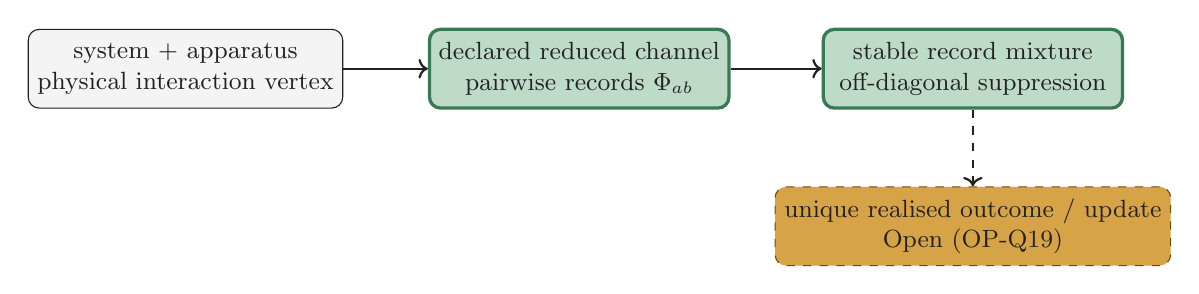
\begin{tikzpicture}[
  box/.style={draw,rounded corners,align=center,minimum width=3.8cm,
    minimum height=1.0cm,font=\small},
  arrow/.style={->,thick,draw=ectInk}]
\node[box,ectExternal] (couple) at (-5.0,0) {system + apparatus\\physical interaction vertex};
\node[box,ectConditional] (channel) at (0,0) {declared reduced channel\\pairwise records $\Phi_{ab}$};
\node[box,ectConditional] (mixture) at (5.0,0) {stable record mixture\\off-diagonal suppression};
\node[box,ectOpen] (open) at (5.0,-2.0) {unique realised outcome / update\\Open (OP-Q19)};
\draw[arrow] (couple) -- (channel);
\draw[arrow] (channel) -- (mixture);
\draw[arrow,dashed] (mixture) -- (open);
\end{tikzpicture}
\caption{Status-separated measurement chain.  A specified interaction and
reduced channel can form stable records; decoherence alone does not supply the
dashed unique-outcome update and does not create Lorentzian signature.  Gray,
green and orange-dashed roles denote supplied, conditional and Open nodes;
literal labels and borders remain decisive in grayscale.}
\label{fig:measurement_EL}
\end{figure}


\subsubsection*{Measurement as environmental locking}

Figure~\ref{fig:measurement_EL} makes the distinction explicit: measurement
is not defined as environmental locking.  A declared channel may form a stable
reduced record, while outcome and update remain Open.


\subsubsection*{The persistent quantum sector as the sector of
minimal environmental coupling}

The persistent quantum sector is not universally the sector of
minimal environmental coupling.  Persistence can arise from symmetry,
kinematic closure, topology, or a small computed width.

\subsubsection*{The photon as a Euclidean traveller}

A photon is a physical gauge-sector excitation after constraint
reduction; the Euclidean-first ontology does not by itself imply zero
decoherence or a special traveller status.
\subsection{Qubit dephasing: a model-specific correlation trade-off}
\label{sec:pes_info_bound}

\textit{Status: Level~A for the algebra of the declared pure-dilation qubit
model; Open for an ECT detector channel and for any protocol-independent
information--disturbance bound.}


\subsubsection*{Derivation for a two-level system}

For a pure-dephasing qubit, the exact reduced-state eigenvalues and
information measures are retained in the owning derivation.  The calculation
tests that source model and does not select an outcome.
Take the initial qubit state
$|\psi\rangle=(|0\rangle+|1\rangle)/\sqrt{2}$ and a pure
system--environment dilation whose reduced channel multiplies the off-diagonal
element by $e^{-\Phi}$, with $\Phi\ge0$.  Then
\begin{equation}
  \rho_S'
  =\frac12
  \begin{pmatrix}
    1 & e^{-\Phi} \\
    e^{-\Phi} & 1
  \end{pmatrix},
  \label{eq:rho_dephased}
\end{equation}
and its eigenvalues are $\lambda_\pm=(1\pm e^{-\Phi})/2$.  The reduced
entropy is therefore
\begin{equation}
  S(\rho_S')
  =h_2\!\left(\frac{1+e^{-\Phi}}{2}\right),
  \qquad h_2(p)=-p\ln p-(1-p)\ln(1-p),
  \label{eq:S_reduced}
\end{equation}
and, because the joint state is pure in this particular dilation,
\begin{equation}
  I(S{:}E)=2S(\rho_S')
  =2h_2\!\left(\frac{1+e^{-\Phi}}{2}\right).
  \label{eq:info_decoherence}
\end{equation}
For $\Phi\ll1$,
\begin{equation}
  I(S{:}E)=\Phi\ln\frac{2e}{\Phi}
  +O\!\left(\Phi^2|\ln\Phi|\right),
  \label{eq:info_small_gamma}
\end{equation}
whereas $I(S{:}E)\to2\ln2$ as $\Phi\to\infty$.

Equation~\eqref{eq:info_decoherence} is a monotonic relation between total
system--environment mutual information and residual qubit coherence
$V=e^{-\Phi}$ under the assumptions just stated.  It is not, by itself, a
bound on accessible classical information, detector readout capacity,
single-copy tomography, collapse, or selection of one outcome.  A mixed
environment, a different dilation, feedback, sequential weak measurements,
or a specified detector POVM changes the operational information question.
No value such as $\Phi=1$, the one-bit point, or the CHSH visibility marker is
a universal quantum--classical boundary.
Numerical evaluations of this same declared toy channel, including the
one-bit and Werner-visibility markers with their scope guards, are tabulated
in Appendix~\ref{app:qubit_numerics}.

\subsubsection*{Sequential weak interactions}
If independent pure-dephasing steps multiply the same off-diagonal element,
their exponents add,
\begin{equation}
  V_N=\prod_{i=1}^{N}e^{-\Phi_i}
  =e^{-\sum_i\Phi_i}.
\end{equation}
The final-state mutual information then follows from
Eq.~\eqref{eq:info_decoherence} with
$\Phi=\sum_i\Phi_i$, provided the total dilation remains pure.  Correlated
environments, feedback, adaptive measurements, and detector readout change
this relation.  Thus the additive statement is a conditional channel result,
not a protocol-independent weak-measurement bound or a tomography theorem.

An ECT application must derive the physical record operator, environmental
state, channel, and readout protocol.  Until those inputs are supplied, this
calculation is a source/model example and provides neither an ECT prediction
nor an ECT-specific measurement theorem (OP-PES-6/OP-Q19).


\subsubsection*{Weak measurements}

Weak measurements are described by the declared pre-selection,
interaction, and post-selection.  Their anomalous weak values do not provide
a protocol-independent probe of an ECT selection scalar.

\paragraph{Can one observe without collapse?}

Observation without a projective update is possible through weak
or nondemolition protocols, but the information--disturbance tradeoff remains
owned by the channel.  Reduced dephasing is not synonymous with collapse.
Figure~\ref{fig:qubit_info_decoherence} displays the exact toy-channel relation
and its explicitly non-universal markers.
\begin{figure}[H]
\centering
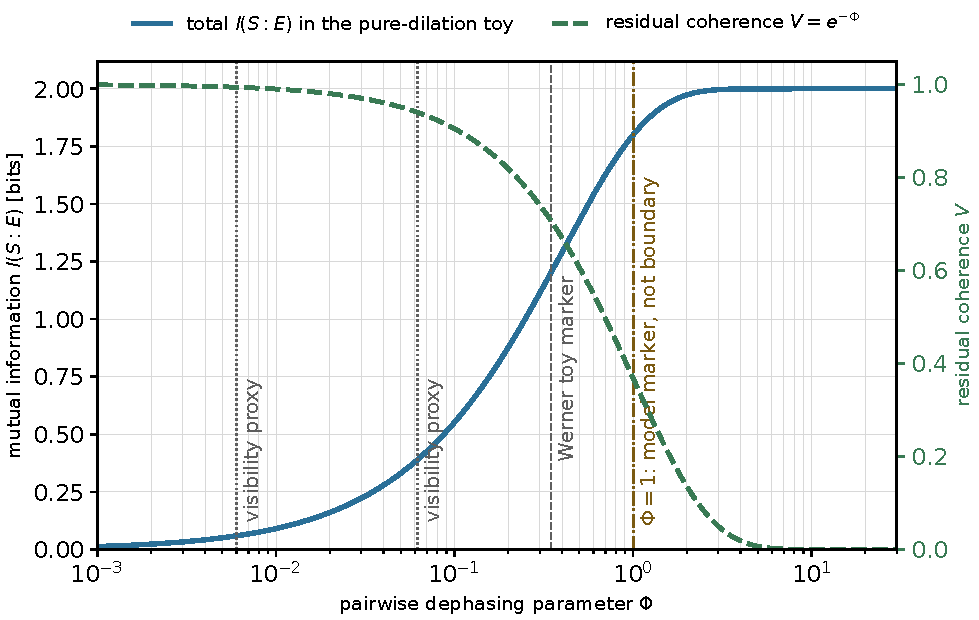
\includegraphics[width=0.90\textwidth]{figures/r155/fig_qubit_info_decoherence_r155.pdf}
\caption{Pure-dilation qubit toy.  The blue solid curve is the
unchanged total mutual information and the green dashed curve is the
unchanged residual coherence.  Vertical lines are explicitly labelled proxy
or toy markers, not collapse, outcome or metric-signature boundaries.  \textit{Display semantics: \detokenize{Both continuous traces are analytic relations of the declared pure-dilation toy; no sampled-data markers are implied.}}}
\label{fig:qubit_info_decoherence}
\end{figure}


\paragraph{Scope and open status.}

The scope is limited to source-model record formation and
finite-time retention.  A universal measurement law, Born rule, and unique
outcome remain Open.

\paragraph{Euclidean meaning of the reverse segments.}

Euclidean reverse segments are not inferred from recoherence.
Where reverse-oriented saddles exist, their weights belong to the system
boundary-value problem, not to a dephasing exponent.

\paragraph{Medium reading~(P5).}

P5 supplies an ontological motivation for common-medium
correlations, while all operational measurement statements still require
normalised physical modes and apparatus couplings.

\paragraph{Connection to decoherence and the arrow-of-time programme.}

Record formation can contribute to an operational arrow for a
specified apparatus but does not prove a cosmological thermodynamic arrow.
The two questions remain separated.

\paragraph{Discriminant: ECT boundary versus standard decoherence
crossover.}

A quantum--classical crossover is channel- and protocol-dependent.
ECT differs from a standard source model only after a condensate calculation
predicts a held-out correction.

\paragraph{Falsifier for the quantum--classical boundary programme.}

The programme fails if a derived ECT channel contradicts
interference, recoherence, or no-signalling data.  It is not falsified by the
failure of an unowned universal threshold, which is no longer claimed.

\paragraph{Empirical anchor.}

C$_{60}$ visibility, photonic coherence, and qubit/cavity data are
retained as empirical source-model anchors.  Their agreement is not evidence
for ECT until the ECT channel is derived.

\paragraph{Bridge to the probability and measurement analysis.}

The bridge to probability requires a separately justified measure
on alternatives.  Pairwise dephasing changes accessibility of interference,
not the origin of Born weights.
\subsection{Probability, Born-type interpretation, and measurement status}
\label{sec:qs_born}\label{sec:born_rule}
% ============================================================
% NOTE: GPT draft used label sec:qs_probability; changed to sec:qs_born
% for consistency with the roadmap in Section~\ref{sec:qs_intro}.

\textit{Status: Level~A mathematics for distinguishing amplitudes,
reduced-state dephasing, diagonal weights, and a separately admitted
probability measure in supplied models.  A physical ECT decoherence channel is
Level~B/Open until its coupling, state, kernel, trace, and timescale are
derived.  The projector version of Gleason gives a conditional representation
theorem only for a supplied complex Hilbert space of dimension at least three
and a normalised, noncontextual, countably additive measure on orthogonal
projector decompositions; dimension two instead requires the separately
declared C2q effect-measure hypotheses stated below.
The physical preparation/state, Born measure, event map, outcome/update rule,
and measurement channel remain Open.  Connections: Sections~\ref{sec:qs_wave},
\ref{sec:qs_ccr}, \ref{sec:qs_reflection_positivity},
\ref{sec:qs_unitarity_status}, \ref{sec:qs_decoherence}, and
\ref{sec:quantum_classical_boundary}.}

\medskip
The previous subsections introduced supplied wave-dynamical and
canonical templates and analysed dephasing inside declared reduced-state
models.  They did not derive a physical ECT macroscopic decoherence channel.
Such a channel still needs an owned coupling, state, influence/noise kernel,
trace, and finite timescale.  Even when those inputs suppress specified
coherences, dephasing neither creates a probability measure nor selects an
outcome.  The separate question below is what standard conditional mathematics
says after Hilbert/projector and probability inputs are admitted.

\paragraph{Physical picture: the probability gap.}
In standard quantum mechanics the Born rule
$P=|\langle\psi|\phi\rangle|^2$ is postulated.  In the present ECT
construction a declared environment can suppress interference between
specified reduced alternatives, but that dephasing neither creates a
probability measure nor chooses one outcome.  A complete applicable corrected
OS-II package can reconstruct a positive quadratic Hilbert norm in a supplied
subsector; reflection positivity alone is insufficient, and neither result
identifies diagonal matrix elements with physical frequencies.  The physical
state/preparation, event map, probability origin, outcome and update therefore
remain Open reconstruction targets.

\paragraph{Inputs to the conditional measure representation.}
For clarity, the discussion separates ordinary C1/C2 projector hypotheses,
the alternative C2q effect-measure hypotheses in dimension two, and the C3
physical-application input; OS-II reconstruction and
dephasing are not Gleason premises:
\begin{enumerate}[leftmargin=*,label={}]
  \item[\textbf{(C1)}] a complex Hilbert space and projector event algebra are
    supplied, with \(\dim\mathcal H\ge3\) for the ordinary projector theorem;
  \item[\textbf{(C2)}] a normalised, noncontextual, countably additive
    probability measure is supplied on every orthogonal projector
    decomposition in the ordinary theorem's domain;
  \item[\textbf{(C2q)}] for \(\dim\mathcal H=2\), a separately supplied
    generalised measure \(v\) is defined on the full effect set
    \(\mathcal E(\mathcal H)=\{E:0\le E\le I\}\), obeys
    \(0\le v(E)\le1\), \(v(I)=1\), and is sigma-additive for every countable
    sequence of effects whose operator sum is at most \(I\).  Normalised POVM
    decompositions with sum \(I\) are the corresponding special case.  These
    are the separately declared C2q hypotheses used by Busch's effect version
    of Gleason's theorem~\cite{Busch2003Gleason};
  \item[\textbf{(C3)}] the physical preparation/state is supplied, together
    with the identification of mathematical projectors (ordinary C2 route),
    or effects/POVM outcomes (C2q route), with laboratory events.  The applicable theorem
    produces a representing density operator for the admitted measure, but
    does not derive which physical preparation it represents.
\end{enumerate}
A different dimension-two representation theorem would require its own
separately declared premises and is not used here.
An independently specified record or dephasing channel may help identify an
approximately orthogonal event algebra in an application, but it is not a
premise of either representation theorem.  ECT does not yet derive (C1),
(C2), (C2q), or (C3) from the bare postulates.  Under (C1)--(C2), ordinary
projector Gleason fixes the representation in complex dimension at least
three.  Under the separately declared (C1)+(C2q) hypotheses, the Busch effect
route supplies the dimension-two representation.  The supplied preparation
plus projector/effect event map (C3) is still required for a physical
application.  None of these steps is a dynamical ECT derivation of
probabilities.

\paragraph{Kochen--Specker boundary.}
The Kochen--Specker theorem separately obstructs a global noncontextual $0/1$
assignment to projectors that assigns exactly one value~1 in every orthonormal
resolution of the identity, in Hilbert-space dimension at least
three~\cite{KochenSpecker1967}.  It is not a premise of the Bell--CHSH or MDL
bounds and neither supplies Born probabilities nor excludes contextual,
nonlocal or measurement-dependent completions.  Applying this gate to ECT
would first require a physical observable algebra, compatible measurement
contexts and an event/value map; those owners remain Open.

\paragraph{Medium reading~(P5).}
P5 motivates seeking amplitudes, environment channels and detector records in
one medium.  It does not establish an amplitude-to-probability transition.
Tracing unresolved modes can dephase a supplied reduced state, but the
probability measure, event algebra and outcome rule remain separate owners.

\paragraph{Connection to the global/reduced unitarity distinction.}
The probability question is logically independent of the global/reduced
unitarity distinction~(\S\ref{sec:qs_unitarity_status}); decoherence can make a
supplied density operator approximately diagonal without creating the measure
used to read its entries.
Standard global unitary dynamics is established only in supplied subsectors
for which the complete applicable corrected OS-II package and reconstruction
are in place; reflection positivity alone is insufficient, and the interacting
full-theory statement remains Open.
The conditional measure-representation discussion begins only after a
normalised, noncontextual, countably additive projector measure has been
independently admitted.  Approximate diagonality identifies a
possible record basis in a specified channel, not the probability or outcome
law.

\subsubsection*{Amplitude versus probability}

Within the supplied coherent closure used in this section, the
bookkeeping objects are amplitudes with weights of the
form~\eqref{eq:qs_weight_S0},
\[
  \mathcal{A}[\theta]
  \sim
  \exp\!\left(\frac{i\,\Sigma_\theta\mathcal I_{\theta,L}[\theta]}{S_0}\right),
\]
and their declared superposition over admissible histories.  This is an EFT
input, not a derivation of the amplitude space, measure, or state from DP.  In
regimes where those supplied sectors interfere, their description remains
amplitude-based; no probability or outcome interpretation follows.

One specified record protocol may proceed from a supplied amplitude/state to a
reduced description in which selected coherences are suppressed.  This gives
diagonal weights, not probabilities.  For that supplied protocol the
bookkeeping is
\begin{equation}
  \begin{aligned}
    \text{supplied amplitudes and state}
    &\;\longrightarrow\;
    \text{specified reduced-state dephasing} \\
    &\;\longrightarrow\;
    \text{diagonal weights}.
  \end{aligned}
  \label{eq:qs_prob_logic}
\end{equation}
This is not a universal temporal or logical order.  An additive probability
measure is an independent premise and may be formulated without decoherence;
the physical ECT channel, event interpretation, and outcome/update remain
Open.

\subsubsection*{Why specified dephasing is not the Born rule}

A declared system--environment channel can make selected off-diagonal reduced
terms small under its stated assumptions.  That calculation does not explain
why diagonal weights are probabilities or why their law is quadratic.  An
approximately diagonal supplied density matrix is therefore neither a
derivation of Born's rule nor an ECT-owned probability mechanism.

This distinction must remain explicit.
Many discussions conflate four conceptually separate steps:
\begin{enumerate}[label=(\roman*)]
  \item suppression of interference;
  \item emergence of classical alternatives;
  \item assignment of probabilities;
  \item the specific quadratic weighting rule.
\end{enumerate}
In ECT these four steps are kept conceptually distinct.

\subsubsection*{Ordinary projector-Gleason representation of an independently supplied measure}

A Born-type probability law is not derived from first principles in ECT.
The present comparison keeps four separately owned layers distinct:
\begin{enumerate}[label=(\roman*)]
  \item a supplied coherent amplitude and action scale;
  \item a supplied norm-preserving complex dynamics;
  \item the ordinary projector hypotheses (C1)--(C2), or the dimension-two
    effect hypotheses (C1)+(C2q), plus the supplied preparation and
    projector/effect event map (C3);
  \item an optional specified reduced-state dephasing channel used only at the
    application/record layer, whose physical ECT owner remains Open.
\end{enumerate}
The applicable representation theorem under (C1)--(C2), or under the
separately declared (C1)+(C2q) hypotheses, is conditionally unique; the physical preparation, event map, probability premise, record
channel, and outcome are not generated by the theorem.  In the projector
theorem's domain there is a unique positive trace-one operator \(\rho_\mu\)
representing the admitted measure.  If (C3) supplies a normalised pure
preparation \(\rho_\mu=|\Psi\rangle\langle\Psi|\) and a rank-one event
\(P_\alpha=|\phi_\alpha\rangle\langle\phi_\alpha|\), then
\begin{equation}
  \label{eq:qs_born_candidate}
  \mu(P_\alpha)
  = \mathrm{Tr}(\rho_\mu P_\alpha)
  = |\langle\phi_\alpha|\Psi\rangle|^2.
\end{equation}
This is the standard representation of the admitted measure.  It is not
produced by dephasing and does not identify a physical branch or realised
outcome without the missing event and update owners.

\paragraph{Status of Eq.~\eqref{eq:qs_born_candidate}:
conditional Gleason representation.}
For a complex Hilbert space of dimension at least three, assumptions
(C1)--(C2) place the admitted measure in the domain of Gleason's
theorem~\cite{Gleason1957}.  The measure then has the unique representation
\(\mu(P)=\mathrm{Tr}(\rho_\mu P)\) by a positive trace-one operator.
The ordinary projector theorem does not cover a two-dimensional Hilbert
space; a qubit statement requires the separately stronger Busch effect/POVM extension under separately declared C2q hypotheses.  Under the complete chosen hypotheses there is no extra
functional-form freedom in the representation.

\textit{What this establishes:}
Gleason gives a conditional representation theorem.  Once the relevant
Hilbert/projector structure, dimension, normalised noncontextual countable
additivity, and theorem domain are supplied, the representing form is fixed.
This is Level~A mathematics inside the stated theorem, not the physical origin
of the measure, state, events, or outcomes.

\textit{What this does not establish:}
ECT has not yet derived the full Hilbert/projector event structure,
probability measure, or physical preparation map from bare P1--P6.
The Gleason representation applies \emph{conditional} on (C1)--(C2), and its
physical reading additionally depends on (C3).
The physical ECT Born rule therefore remains Open~(OP-Q7).  Only the
conditional Gleason form, after its probability assumptions are supplied,
is Level~A mathematics inside that stated model.

\subsubsection*{OS-II Hilbert-norm layer and its separation from probability}

The decision-theoretic routes of Deutsch~\cite{Deutsch1999} and
Wallace~\cite{Wallace2012} obtain quadratic weights from rationality axioms
in a branching quantum world.  Zurek's distinct envariance
route~\cite{Zurek2005} argues from entangled-state symmetries and its own
probability assumptions.
In ECT a quadratic \emph{norm} can be reconstructed conditionally from a
supplied Euclidean model only when its complete applicable corrected OS-II
package holds.  Reflection positivity is one necessary hypothesis, not the
full reconstruction package or a Gleason premise.  Calling the norm a
probability still requires the independent probability assumptions listed
above.

A supplied Euclidean condensate functional
measure~\eqref{eq:qs_euclidean_measure} is one input from which the quadratic
Hilbert structure can be reconstructed under the complete applicable
corrected OS-II package.
For functionals $F$,~$G$ supported in the half-space $w>0$,
the OS route~(\S\ref{sec:qs_reflection_positivity}) defines a
physical inner product:
\begin{equation}
  \label{eq:qs_rp_inner_product}
  \langle F | G \rangle_{\rm OS}
  = \frac{1}{Z_\mu}\int \mathcal{D}\Phi\;
  (\Theta F[\Phi])^*\,G[\Phi]\;
  e^{-\mathcal I_E^\mu[\Phi]} .
\end{equation}
This is the OS form of the supplied measure.  Calling its completion physical
requires the remaining OS-II and observable/clock maps; the measure exponent
does not contain the canonical $S_0$ unless a separate owner map is proved.
This inner product is quadratic in the amplitudes by
construction: it is a defining property of the Euclidean measure
and the reflection operation, not an auxiliary assumption about
probability.
RP guarantees a positive semi-definite OS form.  Quotienting its null states
and completing gives a mathematical Hilbert space for that form; identifying
it as the reconstructed physical Hilbert space $\mathcal{H}_{\rm phys}$ with
time-translation dynamics requires the complete applicable corrected OS-II
package and the physical observable/clock map.

Once the OS-reconstructed Hilbert space is in place, the diagonal
elements of a reduced density matrix are automatically of the form
\begin{equation}
  \label{eq:qs_rp_diagonal}
  \rho_{\alpha\alpha}
  = \langle \alpha | \hat\rho | \alpha \rangle
  = |\langle \alpha | \Psi \rangle|^2
  \qquad \text{(pure state)}.
\end{equation}
This is an algebraic pure-state diagonal identity in the RP-defined inner
product, not a probabilistic theorem.  The diagonal matrix elements inherit
the quadratic structure of~$\langle\cdot|\cdot\rangle_{\rm phys}$, while
their interpretation as normalised physical probabilities remains an
additional step.

The conditional comparison chain is therefore:
\begin{equation}
  \label{eq:qs_born_chain}
  \begin{aligned}
  \underbrace{\mathcal I_E^\mu,\;d\mu,\;\Theta,\;
      \mathcal A_{\rm obs}}_{\text{supplied Euclidean/OS inputs}}
  &\;\xrightarrow{\substack{\text{complete applicable}\\
      \text{corrected OS-II package}}}\;
  \underbrace{\mathcal{H}_{\rm phys},\;
    \langle\cdot|\cdot\rangle}_{\text{quadratic}},\\
  \underbrace{\mathcal{H}_{\rm phys},\;
    \langle\cdot|\cdot\rangle}_{\text{quadratic}}
  &\;\xrightarrow{\text{independent input}}\;
  \underbrace{\substack{\text{projector events}\; +\\
    \text{normalised noncontextual measure}}}_{\text{(C1)--(C2)}},\\
  \underbrace{\substack{\text{projector events}\; +\\
    \text{normalised noncontextual measure}}}_{\text{(C1)--(C2)}}
  &\;\xrightarrow{\text{Gleason representation}}\;
  \mu(P) = \mathrm{Tr}(\rho_\mu P),\\
  \underbrace{\rho_\mu,\;P_\alpha}_{\text{representation}}
  &\;\xrightarrow{\substack{\text{supplied preparation and}\\
      \text{projector/effect event map (C3)}}}\;
  \mu(P_\alpha),\\[-0.2ex]
  \mu(P_\alpha)
  &=|\langle\phi_\alpha|\Psi\rangle|^2
  \qquad\text{for a supplied pure state.}
  \end{aligned}
\end{equation}
For a two-dimensional sector, the projector-measure step is replaced by
the full effect algebra and separately declared C2q hypotheses, giving
\(v(E)=\mathrm{Tr}(\rho_v E)\); C3 then maps effects/POVM outcomes to
laboratory events.  This is a separate theorem domain, not a consequence
of the projector chain.
Dephasing remains a separate reduced-state record step, not a theorem
premise.  The quadratic Hilbert norm is inherited from a complete OS
reconstruction only in the verified subsector; the physical state/event map,
probability premise, and one realised outcome are not inherited from it.

\paragraph{Comparison with decision-theoretic routes.}
The Deutsch--Wallace programme starts from an assumed Hilbert space
and derives the Born rule from rationality constraints on agents.
In supplied Gaussian subsectors, ECT starts from a Euclidean functional
measure and reconstructs a Hilbert norm only under the complete applicable
corrected OS-II package.  A Born probability does not follow without the
separate probability-measure assumptions.  The
Deutsch--Wallace programme is therefore an external comparison, not a step
derived by the present ECT construction.

\paragraph{Residual gap and honest status.}
The RP/OS route narrows the open gap, but it does not close it:
\begin{itemize}[nosep]
  \item \textbf{(C1)}~is available only in explicitly supplied Gaussian
    OS-reconstructed subsectors; the interacting Hilbert/event algebra is a
    constructive target~(OP-Q16);
  \item \textbf{(C2)}~is an independent projector-measure premise in the
    ordinary dimension-at-least-three theorem domain.  Its normalisation,
    noncontextuality, and countable additivity are not derived by RP, OS
    reconstruction, or decoherence;
  \item \textbf{(C2q)}~is the separately supplied full-effect generalised
    measure premise in dimension two, with the positivity, normalisation and
    sigma-additivity hypotheses stated above; it too is not derived by RP,
    OS reconstruction, or decoherence;
  \item \textbf{(C3)}~remains a physical owner problem: neither the prepared
    state nor the laboratory projector or effect/POVM-event identification is selected by
    the representation theorem;
  \item the \textbf{record/dephasing layer} remains independently Open as an
    ECT channel and is not a hypothesis of Gleason's theorem.
\end{itemize}

\paragraph{Level summary for the separate OS-II and Gleason layers.}
\textit{Level~A mathematics under stated hypotheses:}
the complete supplied free-Gaussian corrected OS-II packages and,
independently, ordinary projector Gleason's representation of the admitted
measure under (C1)--(C2), with a qubit handled only by the Busch effect/POVM theorem under separately declared C2q hypotheses.
\textit{Level~B:}
conditional reduced-state dephasing and approximate record sectors for a
declared system--environment split; diagonal identities remain kinematical.
\textit{Open:}
ECT ownership of (C1), (C2) or (C2q), and (C3), the interacting OS completion, the physical
state/preparation and projector/effect event map, the record channel, probability origin, and
the outcome/update rule.

An independently supplied projector measure therefore has only the
conditional Gleason trace representation after the exact theorem hypotheses
are supplied.  This is not a completed ECT Born derivation from P1--P6; the
physical state/preparation, event map, probability origin, outcome and update
remain Open.

\subsubsection*{Reduced density matrix viewpoint}

In a supplied reduced description one may write the schematic matrix
\begin{equation}
  \label{eq:qs_rho_red}
  \rho_{\rm red}(q,q')
  =
  \sum_{\alpha,\beta}
  \Psi_\alpha(q)\,\Psi_\beta^*(q')\,
  \mathcal{D}_{\alpha\beta},
\end{equation}
where $\mathcal{D}_{\alpha\beta}$ is the channel-dependent dephasing factor of
that model.  If its declared coupling, state, kernel, trace, and timescale give
\begin{equation}
  \label{eq:qs_diag_limit}
  \mathcal{D}_{\alpha\beta} \approx 0
  \qquad (\alpha\neq\beta),
\end{equation}
the matrix is approximately diagonal.  Its diagonal entries remain weights,
not probabilities, until an event algebra and probability measure are supplied.

\paragraph{What this does and does not show.}
The calculation shows only dephasing in the specified source model.  It neither
derives a physical ECT channel nor makes a probability interpretation natural
or necessary.  Gleason fixes a trace representation only after (C1)--(C2) are
admitted in their precise theorem domain; its physical Born reading also
requires (C3).  Deriving these inputs, the physical channel, and the
outcome/update rule remains Open.

\subsubsection*{Measurement status}

ECT does not yet contain a completed first-principles measurement
theory.  The manuscript can organise the following supplied bookkeeping
ingredients without claiming their physical derivation: coherent amplitudes,
a specified reduced-state dephasing map, diagonal record weights, and a
conditional Gleason representation after a probability measure is admitted.
The physical coupling, state, kernel, trace, timescale, stable-record map,
probability measure, and outcome/update rule all remain Open; no universal
branching or Born mechanism follows from the displayed chain.

\paragraph{What remains open.}
A full measurement theory would require:
\begin{enumerate}[label=(\roman*)]
  \item a precise branch-selection and state-update rule;
  \item a physical derivation of the state/preparation, event map and
    probability origin from the condensate dynamics;
  \item a treatment of pointer sectors and stable macroscopic records;
  \item control of the r\^ole of defect and topological sectors during
    measurement-like processes~(Section~\ref{sec:qs_defects}).
\end{enumerate}

\subsubsection*{Why the current result is still meaningful}

The present construction usefully separates Hilbert kinematics,
reduced-state dephasing, probability assignment, and outcome selection.
It does not yet explain why physical probabilities exist or why one outcome
is realised.  Its positive result is a scoped conditional comparison route,
not a solution of the Born or measurement problem.

\subsubsection*{Bridge to entanglement and Bell-type correlations}

The probability and measurement discussion has so far used supplied
reduced-state dephasing models and conditional record alternatives.  The next
step analyses the case of supplied coherent correlations that are
non-factorisable and are therefore not exhausted by that conditional
bookkeeping.  Neither the
dephasing model nor an effectively classical alternative is thereby promoted
to an ECT-derived physical channel.
That is the subject of the next section on entanglement and
Bell-type correlations.

\paragraph{Discriminant: ECT conditional measure-representation programme
versus standard probability postulates.}
Standard formulations of quantum theory usually take the Born rule as
an axiom or attempt to justify it through auxiliary principles such as
decision theory.
ECT treats the origin of the physical probability measure as Open.  The
present text organises supplied coherent amplitudes and derives or reproduces
reduced-state dephasing only inside specified source models; the corresponding
physical ECT channel remains Open, and neither step creates a measure.
Ordinary projector Gleason asks what trace form an independently supplied
normalised, noncontextual, countably additive projector measure must take on a
complex Hilbert space with $\dim\mathcal H\ge3$; a qubit requires the Busch effect/POVM theorem under separately declared C2q hypotheses.  The ECT-specific programme is
to derive the missing state/preparation, event, probability-origin, outcome
and update structures from the medium.  At present only the conditional trace
representation is available after those inputs are supplied.

\paragraph{Falsifier for the Born-weight programme.}
The present programme would be weakened if a completed ECT derivation
showed that the physical alternatives do not admit the Hilbert/projector
structure assumed in~(C1), or that the measure premise~(C2) is inconsistent
with the coherent-branch
architecture.
It would be more strongly challenged if a completed derivation forced a
non-quadratic probability rule while retaining the same Hilbert-space
structure.
At present, no such incompatibility is known; the open point is not
inconsistency, but incompleteness.

\paragraph{Empirical status.}
The quadratic Born weighting is extraordinarily well confirmed across
atomic, molecular, optical, and solid-state quantum experiments.
ECT does not claim a distinct experimental prediction at this stage.
Its present contribution is architectural: it identifies precisely which
inputs are needed before the conditional quadratic representation applies.

\statussummary
\textit{Established~(Level~A mathematics in stated models):}
the logical distinction among amplitudes, reduced-state dephasing, diagonal
weights, and an admitted probability measure; complete applicable corrected
OS-II packages for supplied Gaussian subsectors reconstruct a positive
quadratic Hilbert norm but not physical probabilities.

\textit{Conditional theorem:}
under (C1)--(C2), including a complex Hilbert space with
$\dim\mathcal H\ge3$ and normalised noncontextual countable additivity,
ordinary projector Gleason's theorem~\cite{Gleason1957} fixes the trace
representation of the independently admitted measure; a qubit requires the
Busch effect/POVM theorem under separately declared C2q hypotheses.  The physical
application still needs (C3).  OS-II reconstruction is a separate layer and
is not a Gleason premise.

\textit{Open:}
(i)~full interacting RP verification~(OP-Q16);
(ii)~the probability origin/premise~(C2) and physical state,
preparation plus projector/effect event map~(C3);
(iii)~the system--environment coupling, state, kernel, trace, timescale, and
projector/record channel at the independent application layer;
(iv)~the outcome/update rule.

\paragraph{Summary.}
ECT does not postulate probability at the foundation.  A specified supplied
dephasing model can suppress declared coherences, but no physical ECT channel
has yet been derived and dephasing does not create a probability measure or
select an outcome.  Once (C1)--(C2) are independently admitted in the exact
theorem domain, Gleason conditionally fixes the trace representation; a
physical Born application still needs (C3).  The channel, origin of the
measure, physical preparation plus projector/effect event map, actual outcomes, and update rule
remain Open.
The next step is to analyse the case of a supplied coherent correlation
structure that is non-factorisable before branch-based probability language
is invoked.

% ============================================================

\begin{longtable}{@{}L{2.8cm}L{3.5cm}L{3.5cm}L{4.6cm}@{}}
\caption{Comparison of Born-rule justification routes and the ECT conditional
measure-representation programme.} \\
\label{tab:born_comparison} \\[-6pt]
\toprule
Aspect & Deutsch (1999)~\cite{Deutsch1999} &
  Wallace (2012)~\cite{Wallace2012} &
  ECT (this work) \\
\midrule
\endfirsthead
\toprule
Aspect & Deutsch (1999)~\cite{Deutsch1999} &
  Wallace (2012)~\cite{Wallace2012} &
  ECT (this work) \\
\midrule
\endhead
\midrule\multicolumn{3}{r}{\small\textit{(continued on next page)}}\\
\endfoot
\bottomrule
\endlastfoot
Framework
  & MWI + decision theory
  & MWI + decoherence
  & Supplied coherent/dephasing templates + Hilbert norm from a complete
    applicable corrected Gaussian OS-II package + independent ordinary
    projector-Gleason representation of an admitted measure; physical ECT
    owners Open \\
Source of weights
  & Rationality axioms
  & Rationality + branch structure
  & Under (C1)--(C2), or under separately declared (C1)+(C2q)
    hypotheses in dimension two, the admitted measure has a unique trace
    representation; physical use additionally requires the preparation plus
    projector/effect event map~(C3) \\
Origin of quadratic structure
  & Decision-theoretic axiom
  & Rationality + separability
  & Hilbert norm from a specified complete applicable corrected OS-II package
    plus an applicable independently supplied projector measure~(C2), or
    full-effect generalised measure~(C2q) in dimension two; OS-II is not a
    Gleason premise \\
Dephasing / decoherence
  & Not used
  & Postulated
  & Derived or reproduced only inside specified source models with declared
    state, split, coupling, kernel, trace and timescale; physical ECT owner Open
    and not a probability owner \\
Extra assumptions
  & Rationality
  & Rationality + separability
  & (C1)--(C2) for the ordinary projector theorem, or separately declared
    (C1)+(C2q) full-effect hypotheses in dimension two; (C3) supplies the
    preparation plus projector/effect event map \\
Known limitations
  & Circularity~\cite{Barker2000}
  & Albert (2010) objection
  & Conditional representation only; first-principles derivation of
    (C1), (C2) or (C2q), and (C3), the probability owner, and unique outcome selection still
    open (OP-Q19) \\
\hline

\end{longtable}


% ==============================================================
\section{Quantum Entanglement and Bell-Type Correlations}
\label{sec:qs_entanglement}
% ==============================================================

\textit{Status: Level~A standard mathematics for a supplied tensor-product
state/channel and its reduced density operators; ECT ownership Open.  A common
medium alone does not force nonfactorisation.  The physical subsystem/state,
local measurement map, Bell correlators, Tsirelson-type bounds and
no-signalling completion remain Open.
Connection: the Hilbert-space bridge
(\S\ref{sec:qs_reflection_positivity}), the global/reduced unitarity
distinction~(\S\ref{sec:qs_unitarity_status}), the exchange-sector
topology~(\S\ref{sec:qs_statistics}), the decoherence programme
(\S\ref{sec:qs_decoherence}), the vacuum-response infrastructure
(\S\ref{par:vacuum_programme}), the Born-weight route
(\S\ref{sec:qs_born}), medium character~(P5), and the
quantum--classical boundary~(\S\ref{sec:quantum_classical_boundary}).}

\paragraph{Physical picture: entanglement as a trace of a common
configuration.}
In the standard formulation, entanglement is introduced as
mathematical non-factorisability in a tensor product of Hilbert spaces.
ECT may host such a state in a common medium, but common support alone neither
creates a tensor-product Hilbert space nor forces the joint state to be
nonfactorising.  The physical subsystem map, nonfactorising state/channel,
local measurement operators and no-signalling/Bell correlators must be supplied
or derived independently.  A common-medium picture is therefore an
interpretation of an already specified entangled state, not its Level~B
derivation.


\paragraph{Connection to PES-R.}
Shared-medium language is an interpretation of a previously specified joint
state; it does not by itself derive entanglement, Bell correlators, or a
no-signalling theorem.  PES-R may classify the retention and record distinguishability
of modes after the joint Hilbert-space dynamics and subsystem map have been
established.  Neither $\Phi_{ab}\ll1$ nor $\Phi_{ab}\gg1$ defines a metric
signature, an interaction law, or a measurement update.  The ECT derivation
of Bell-inequality-violating correlators and the physical subsystem/record
operators therefore remains Open (OP-Q20/OP-PES-1).

\paragraph{What is established, what is structurally suggested, and what
remains open.}
\label{par:entanglement_programme}
The tensor-product and reduced-state language used below presupposes the
physical Hilbert-space bridge discussed in
Section~\ref{sec:qs_reflection_positivity}.

The existing infrastructure provides only conditional ingredients: specified
Gaussian correlators, influence functionals after a system--environment split,
and standard reduced-state algebra.  These tools can propagate or degrade a
nonfactorising state once it is supplied.  They do not prove that the physical
ECT state is nonfactorising, derive a Born measure, or select local measurement
operators.  The full ECT state/channel and Bell map remain Open.

\paragraph{Medium reading~(P5).}
P5 motivates looking for a common-medium owner, but factorising and
nonfactorising states are both compatible with a common substrate.  No generic
nonfactorisation theorem follows without an interaction, boundary condition or
state-selection rule that fixes the cross-correlators.

\paragraph{No-signalling and operational locality.}
The common-medium reading of entanglement does not imply operational
superluminal signalling.
For a supplied quantum channel, no-signalling and Bell inequalities can be
checked by the standard operational rules.  The present ECT action has not yet
derived that channel, so it claims neither a signalling mechanism nor a
medium-based derivation of Bell violation.

\paragraph{Connection to exchange sectors.}
For systems of indistinguishable excitations, the entanglement
programme is constrained by the exchange-sector topology established in
Section~\ref{sec:qs_statistics}.
The two exchange homotopy classes of a supplied identical-point
configuration space constrain possible representations, but do not select the
physical bosonic/fermionic representation or particle sector.
This does not mean that all entanglement reduces to exchange
structure.
Rather, exchange topology provides part of the kinematical backbone for
entanglement in the indistinguishable-sector case, while the broader
non-factorisable correlation logic applies to distinguishable reduced
subsystems as well.

\paragraph{Minimal structural statement.}
Given a supplied total state,
$\hat\rho_{AB}=\mathrm{Tr}_{\rm env}\hat\rho_{\rm tot}$ may factorise or not;
the trace operation alone decides neither case.  A nonzero connected
cross-correlator or an explicit nonseparable preparation/channel is the required
owner.  Thus ECT currently supplies a place where an entanglement mechanism
could live, but not a theorem that the medium forces nonseparability or Bell
violation.  There is likewise no amplitude $\to$ decoherence $\to$ probability
derivation.

\paragraph{Discriminant with respect to axiomatic QM and local
hidden-variable pictures.}
Three correlation pictures should be kept distinct.
In axiomatic quantum mechanics, entanglement is treated as a primitive
property of the tensor-product state space.
In local hidden-variable models, Bell-violating correlations are
forbidden once factorisability and measurement independence are imposed.
ECT has not yet been placed in either class operationally because its physical
joint state and local measurement map are missing.  A viable completion must
reproduce Bell-type correlations and no-signalling without reducing to an
excluded Bell-local hidden-variable model.

\paragraph{CHSH premise ledger: the common-measure step.}
The standard CHSH conclusion is a theorem about a specified probability
class, not about deterministic language by itself
\cite{Bell1964EPR,CHSH1969,ClauserHorne1974}.  Let
$x,y\in\{0,1\}$ denote settings and $a,b\in\{-1,+1\}$ denote outcomes.
A Bell-factorisable model with measurement independence has
\begin{equation}
  P(a,b\mid x,y)
  =\int_{\Lambda} d\rho(\lambda)\,
    p_A(a\mid x,\lambda)\,p_B(b\mid y,\lambda),
  \qquad
  d\rho(\lambda\mid x,y)=d\rho(\lambda),
  \label{eq:r169_bell_factorisable_common_measure}
\end{equation}
where $d\rho$ is one positive normalised measure for all four setting
pairs.  Define the bounded conditional response means
\begin{equation}
  A_x(\lambda)=\sum_{a=\pm1}a\,p_A(a\mid x,\lambda),
  \qquad
  B_y(\lambda)=\sum_{b=\pm1}b\,p_B(b\mid y,\lambda),
  \qquad |A_x|,|B_y|\leq1 .
  \label{eq:r169_local_response_means}
\end{equation}
Factorisability gives
$E_{xy}=\int d\rho\,A_xB_y$.  With the convention
\begin{equation}
  S=E_{00}+E_{01}+E_{10}-E_{11},
  \label{eq:r169_chsh_convention}
\end{equation}
all four terms may be combined under the same measure:
\begin{align}
  S
  &=\int_{\Lambda}d\rho(\lambda)\,C(\lambda),
  \\
  C(\lambda)
  &=A_0(B_0+B_1)+A_1(B_0-B_1).
  \label{eq:r169_chsh_common_integrand}
\end{align}
For each $\lambda$,
\begin{equation}
  |C(\lambda)|
  \leq |B_0+B_1|+|B_0-B_1|
  =2\max\{|B_0|,|B_1|\}\leq2,
\end{equation}
and therefore
\begin{equation}
  |S|\leq2.
  \label{eq:r169_standard_chsh_bound}
\end{equation}
For deterministic responses $A_x,B_y\in\{-1,+1\}$ the integrand is
exactly $+2$ or $-2$.  Thus the proof uses, separately,
(i)~dichotomic bounded outcomes, (ii)~Bell factorisability of the
conditional responses, and (iii)~one setting-independent probability
measure.  Dropping any one premise removes this particular inference; it
does not by itself select a replacement theory or a value of~$S$.

\paragraph{What a CHSH violation excludes.}
A statistically validated value $|S|>2$ does not rule out hidden variables as
such.  It excludes the Bell-local common-measure class in which one fixed
preparation is represented on a common latent space by one positive
normalised setting-independent measure, bounded outcomes, and Bell-
factorisable response functions used consistently in all four setting
contexts.  Nonlocal, contextual, measurement-dependent, retrocausal,
atemporal global-constraint and selection-dependent hidden-variable
completions are not excluded by this inequality alone.  Conversely, dropping
one premise neither derives the observed quantum correlation set nor proves
operational no-signalling or the Tsirelson ceiling.

The present ECT source has not derived a physical preparation-level latent
variable or quantum state, setting generators, event measure, detector
instruments or complete conditional response law.  It is therefore not
presently classified as Bell-local, nonlocal, measurement-dependent,
retrocausal or superdeterministic.  Bell violation is neither a current
confirmation nor a current falsification of ECT; it is a mandatory external
gate for any completed operational model.

\paragraph{What changes for a setting-dependent measure.}
Suppose the local response maps are retained but the conditional hidden-state
measure is allowed to depend on the joint setting:
\begin{equation}
  P(a,b\mid x,y)
  =\int_{\Lambda}d\rho_{xy}(\lambda)\,
    p_A(a\mid x,\lambda)p_B(b\mid y,\lambda).
  \label{eq:r169_setting_dependent_model}
\end{equation}
The four correlators are then integrals with four measures.  They may be
represented relative to a common dominating measure, but in general with four
different Radon--Nikodym weights; the single common-weight pointwise CHSH
integrand~\eqref{eq:r169_chsh_common_integrand} is therefore unavailable.  Hence
$d\rho_{xy}\neq d\rho$ invalidates the common-measure proof of
Eq.~\eqref{eq:r169_standard_chsh_bound}.  This statement is only logical:
setting dependence permits but does not guarantee a violation, and a
statistical dependence $P(\lambda\mid x,y)\neq P(\lambda)$ does not identify
whether its physical explanation, if any, is a common cause, retrocausal
influence, global constraint, contextual preparation, or selection effect.

\paragraph{Explicit 16-state construction: a Tsirelson-value target.}
The following is a generic finite probability construction, not a model
derived from ECT.  Related measurement-dependent locally factorisable
deterministic models are known independently of ECT
\cite{Hall2010MeasurementIndependence}.  Take
\begin{equation}
  \Lambda=\{-1,+1\}^4,
  \qquad
  \lambda=(\alpha_0,\alpha_1,\beta_0,\beta_1),
  \qquad
  A_x(\lambda)=\alpha_x,
  \quad B_y(\lambda)=\beta_y .
  \label{eq:r169_sixteen_state_space}
\end{equation}
The response at each wing is deterministic and depends only on the local
setting once $\lambda$ is fixed.  Let
$\eta_{00}=\eta_{01}=\eta_{10}=+1$, $\eta_{11}=-1$, and
$c=1/\sqrt2$.  For each setting pair define
\begin{equation}
  \rho^{(T)}_{xy}(\lambda)
  =\frac{1+c\,\eta_{xy}\alpha_x\beta_y}{16}.
  \label{eq:r169_tsirelson_target_measure}
\end{equation}
Because $|c|\leq1$, every weight is non-negative.  Summation over the 16
states gives
\begin{equation}
  \sum_{\lambda}\rho^{(T)}_{xy}=1,
  \qquad
  \langle A_x\rangle_{xy}=\langle B_y\rangle_{xy}=0,
  \qquad
  E_{xy}=c\eta_{xy}.
  \label{eq:r169_tsirelson_target_checks}
\end{equation}
Consequently
\begin{equation}
  S=4c=2\sqrt2,
  \qquad
  P(A=a\mid x,y)=P(B=b\mid x,y)=\frac12.
  \label{eq:r169_tsirelson_target_result}
\end{equation}
The last identities verify operational no-signalling for these four finite
distributions, but do not supply a causal explanation of them.

For the total-variation convention
\begin{equation}
  M_{\rm TV}
  =\max_{s,t}\operatorname{TV}(\rho_s,\rho_t),
  \qquad
  \operatorname{TV}(p,q)
  =\frac12\sum_{\lambda}|p(\lambda)-q(\lambda)|,
  \label{eq:r169_tv_definition}
\end{equation}
the signed products
$\eta_{xy}\alpha_x\beta_y$ associated with two distinct setting pairs
differ on eight of the 16 states.  Therefore
\begin{equation}
  M_{\rm TV}=\frac{c}{2}=\frac{1}{2\sqrt2}.
  \label{eq:r169_tsirelson_target_tv}
\end{equation}
This value characterises this construction under the declared TV convention;
it is not claimed to be a minimal measurement-dependence cost.

\paragraph{Counterexample: setting dependence without Bell violation.}
On the same state space and with the same local deterministic responses, set
\begin{equation}
  \widetilde\rho_{xy}(\lambda)
  =\frac{1+\tfrac12\alpha_{1-x}\beta_{1-y}}{16}.
  \label{eq:r169_subcritical_measure}
\end{equation}
These four measures are setting dependent, non-negative and normalised, but
they correlate only the response bits not sampled at the chosen pair.
Direct summation gives
\begin{equation}
  E_{00}=E_{01}=E_{10}=E_{11}=0,
  \qquad S=0,
  \qquad M_{\rm TV}=\frac14,
  \label{eq:r169_subcritical_result}
\end{equation}
with uniform one-party marginals.  Thus violation is not a consequence of
setting dependence alone.

\paragraph{A TV-controlled sufficient bound.}
The failure of the common-measure proof can be quantified without assigning a
physical mechanism.  Choose $\rho_{00}$ as a reference and add and subtract
it in the other three terms:
\begin{align}
  S={}&\int d\rho_{00}\,
  \bigl[A_0B_0+A_0B_1+A_1B_0-A_1B_1\bigr]
  \\
  &+\int(d\rho_{01}-d\rho_{00})A_0B_1
   +\int(d\rho_{10}-d\rho_{00})A_1B_0
   -\int(d\rho_{11}-d\rho_{00})A_1B_1 .
  \label{eq:r169_tv_bound_decomposition}
\end{align}
For $|f|\leq1$,
$|\int f\,d(p-q)|\leq2\operatorname{TV}(p,q)$.  The first line of
Eq.~\eqref{eq:r169_tv_bound_decomposition} has magnitude at most two, so
\begin{equation}
  |S|
  \leq 2+2\!\left[
    \operatorname{TV}(\rho_{01},\rho_{00})
   +\operatorname{TV}(\rho_{10},\rho_{00})
   +\operatorname{TV}(\rho_{11},\rho_{00})\right]
  \leq2+6M_{\rm TV}.
\end{equation}
Combining this with the algebraic ceiling gives the sufficient general bound
\begin{equation}
  |S|\leq\min\{4,\,2+6M_{\rm TV}\}.
  \label{eq:r169_tv_chsh_bound}
\end{equation}
No tightness claim is made.  The bound also holds for stochastic
factorisable responses because the conditional response means remain in
$[-1,1]$.

\paragraph{Measurement-dependence metrics and the corrected Hall
comparison.}
Hall's joint $L^1$ diameter $M_{\rm H}$ and the total-variation diameter used
here obey $M_{\rm H}=2M_{\rm TV}$.  In Hall's deterministic no-signalling
model class the relaxed CHSH relation is~\cite{Hall2011RelaxedBell}
\begin{equation}
 |S|\leq\min\{2+3M_{\rm H},4\}
       =\min\{2+6M_{\rm TV},4\}.
 \label{eq:r174_hall_exact_bound}
\end{equation}
Consequently, within that declared class,
\begin{equation}
 M_{\rm TV}\geq
 \max\!\left\{0,\frac{|S|-2}{6}\right\}.
 \label{eq:r174_tv_resource_floor}
\end{equation}
The four-setting targets are
\begin{equation}
 \begin{array}{c|c|c}
  \text{target} & M_{\rm H} & M_{\rm TV} \\
  \hline
  |S|=2\sqrt2 & 2(\sqrt2-1)/3 & (\sqrt2-1)/3\simeq0.138071,\\
  |S|=4       & 2/3             & 1/3.
 \end{array}
 \label{eq:r174_hall_two_targets}
\end{equation}
The $1/3$ value is therefore the cost of the algebraic maximum in this
metric, not of the quantum maximum.

The published erratum to Hall's explicit model for the full continuum of
projective singlet correlations~\cite{Hall2016Erratum} corrected its global diameter to
$M_{\rm H,singlet}\simeq0.276434$, or
\begin{equation}
 M_{\rm TV,singlet}\simeq0.138217,\qquad
 F_{\rm singlet}=1-M_{\rm TV,singlet}\simeq0.861783
 \label{eq:r174_hall_erratum_values}
\end{equation}
Thus the often quoted
approximately $14\%$ statement means $1-F=M_{\rm TV}\simeq0.1382$ in Hall's
convention.  It is not a setting-predictability probability, mutual
information or a universal fraction of free choice.  The corrected full-
singlet construction is close to, but does not exactly saturate, the four-
setting floor above.  The finite construction in
Eq.~\eqref{eq:r169_tsirelson_target_measure}, with
$M_{\rm TV}=1/(2\sqrt2)$, is nonminimal and is not ECT physics.

Mutual-information measures quantify a different resource.  Barrett and Gisin
constructed Bell-local correlated-setting models reproducing all projective
singlet correlations while Bob's setting remains independent of the latent
variable and with at most one bit of mutual information between Alice's
setting and the latent variable~\cite{BarrettGisin2011MeasurementIndependence}.
This is a model-class existence upper bound, not a proved minimum, a conversion
to $M_{\rm TV}$ or $(\ell,h)$, or an ECT parameter.

\paragraph{Measurement-dependent-local inequalities as a future test.}
A bounded measurement-dependent-local (MDL) class may instead be defined by
\begin{equation}
 \ell\leq P(x,y\mid\lambda)\leq h
 \label{eq:r174_mdl_setting_bounds}
\end{equation}
for every allowed setting pair and latent state.  The resulting behaviours
form a convex polytope with Bell-like inequalities adapted to the declared
bounds.  For every strictly positive lower bound $\ell>0$, suitable quantum
correlations escape that MDL polytope~\cite{PutzEtAl2014MDL}; this result does
not cover unrestricted dependence with $\ell=0$.

Two experiments illustrate that this bounded class is empirically testable.
Using the additional observed-setting condition $P(x,y)=1/4$, Aktas
\emph{et al.}\ violated the corresponding MDL inequality with a partially
entangled photon pair.  Their data gave violations for
$\ell_{\rm raw}>0.090(4)$ and, after accidental-count subtraction,
$\ell_{\rm net}>0.074(6)$~\cite{AktasEtAl2015MDLExperiment}.  The detection
and locality loopholes remained open, and settings were changed only between
successive run series.  Liu \emph{et al.}\ later used human-generated
real-time settings and spacelike-separated measurement sites, reporting an
MDL violation incompatible with the declared local models for
$\ell>0.10\pm0.05$ under their protocol assumptions
\cite{LiuEtAl2019MDLExperiment}.  These are external exclusions within
specified bounded MDL classes: they do not measure a physical $\ell$, cover
unrestricted dependence with $\ell=0$, or supply an ECT mechanism.

For ECT, Eq.~\eqref{eq:r174_mdl_setting_bounds} is a future falsification
framework, not a present mechanism.  The theory would first have to derive
the preparation-level $\lambda$, setting generators, stable values or bounds
for $\ell,h$, the complete $P(a,b,x,y\mid\mathsf p)$, detector/selection map
and likelihood.  There is no model-independent conversion between
$M_{\rm TV}$ and $(\ell,h)$ without additional assumptions.

\paragraph{No-signalling does not supply the Tsirelson bound.}
Replacing $c=1/\sqrt2$ by $c=1$ in
Eq.~\eqref{eq:r169_tsirelson_target_measure} preserves positivity,
normalisation and exactly uniform one-party marginals, but yields
$S=4$.  Thus a setting-dependent local-response construction may be
operationally no-signalling and still exceed $2\sqrt2$.  The value
$2\sqrt2$ in Eq.~\eqref{eq:r169_tsirelson_target_result} was selected as a
target; it was not derived.  In standard quantum mathematics the Tsirelson
bound instead follows when one positive normalised state owns all four
correlators and the Bell observables are bounded self-adjoint projective
dichotomic observables (Hermitian unitaries),
\[
  \widehat A_x^\dagger=\widehat A_x,\qquad
  \widehat B_y^\dagger=\widehat B_y,\qquad
  \widehat A_x^2=\widehat B_y^2=\mathbb I,
  \qquad
  [\widehat A_x,\widehat B_y]=0
  \quad\hbox{for all }x,y .
\]
For
\begin{equation}
  \widehat{\mathcal S}
  =\widehat A_0(\widehat B_0+\widehat B_1)
   +\widehat A_1(\widehat B_0-\widehat B_1),
\end{equation}
$\widehat{\mathcal S}$ is self-adjoint and the standard identity
\[
  \widehat{\mathcal S}^{\,2}
  =4\mathbb I-[\widehat A_0,\widehat A_1]
                 [\widehat B_0,\widehat B_1]
\]
holds.  Hermitian unitarity gives
$\|[\widehat A_0,\widehat A_1]\|\leq2$ and
$\|[\widehat B_0,\widehat B_1]\|\leq2$, hence
\[
  \|\widehat{\mathcal S}\|^2
  =\|\widehat{\mathcal S}^{\,2}\|
  \leq8,
  \qquad
  \|\widehat{\mathcal S}\|\leq2\sqrt2 .
\]
Therefore every one common positive normalised state $\omega$ obeys
$|\omega(\widehat{\mathcal S})|\leq2\sqrt2$
\cite{Cirelson1980,PopescuRohrlich1994}.  The involution identities
$\widehat A_x^2=\widehat B_y^2=\mathbb I$ without self-adjointness are not
sufficient for this norm proof.  ECT would have to derive the physical state,
operator algebra and locality map entering the stated hypotheses, or derive
another comparably restrictive principle; the finite construction does
neither.

\paragraph{Three CHSH ceilings and one common quantum state.}
The local Bell bound, the quantum Tsirelson bound and the algebraic bound,
\begin{equation}
 |S|\leq2,\qquad |S|\leq2\sqrt2,\qquad |S|\leq4,
 \label{eq:r174_three_chsh_ceilings}
\end{equation}
answer different questions.  The first follows from the Bell-local
common-measure assumptions above.  The second follows when one positive
normalised state owns all four Bell-operator words and the bounded
self-adjoint dichotomic and cross-party commutation hypotheses in the
preceding paragraph hold.  Four
positive setting-conditioned states need not combine into that single
functional.  The third is the algebraic maximum and is compatible with
no-signalling tables outside the standard quantum set.

The Osterwalder--Schrader programme is a conditional route to a positive
Hilbert-space representation, not by itself a Bell completion.  It requires
the complete applicable reconstruction package and one physical
preparation, local observable algebras, detector effects, event map and
setting protocol.  Reflection positivity of separate context-conditioned
measures does not manufacture the common Bell state.  Conversely, an
OS/Hilbert representation and a contextual or setting-dependent hidden-state
representation are not logical negations: the same operational table may
admit more than one representation.  A future ECT completion must derive why
its full correlation family lies inside the quantum ceiling rather than
merely selecting one value of $S$.

\paragraph{Conditional global-configuration template for ECT.}
The Euclidean boundary-value character of the bare model motivates a precise
question but does not answer it.  Let $\mathsf p$ denote a physical
preparation, let $[\Gamma]\in\mathfrak C_{\rm phys}$ denote a complete global
configuration after all applicable constraints and gauge identifications,
and let $x,y$ denote physical apparatus settings.  If a positive normalised
conditional measure and gauge-invariant record maps were supplied, one could
write
\begin{equation}
  E^{\rm glob}_{xy}
  =\int_{\mathfrak C_{\rm phys}}
    d\mu_{\mathsf p,xy}([\Gamma])\,
    \mathcal A_x([\Gamma])\mathcal B_y([\Gamma]),
  \qquad
  |\mathcal A_x|,|\mathcal B_y|\leq1.
  \label{eq:r169_ect_global_measure_template}
\end{equation}
For deterministic records the two maps take values $\pm1$.  A possible
mathematical construction would be a push-forward
\begin{equation}
  \mu_{\mathsf p,xy}
  =(F_{\mathsf p,xy})_{\#}\nu_{\mathsf p},
  \label{eq:r169_ect_pushforward_template}
\end{equation}
where $F_{\mathsf p,xy}$ is a well-posed solution map from unresolved
admissible boundary data to a global physical configuration and
$\nu_{\mathsf p}$ is a declared probability law on those data.  Neither
$F_{\mathsf p,xy}$ nor $\nu_{\mathsf p}$ is presently a physical ECT owner.
In particular, a Euclidean action weight, an influence functional, a reduced
state, practical ignorance, or PES-R bookkeeping does not by itself provide
the positive experimental probability measure in
Eq.~\eqref{eq:r169_ect_global_measure_template}.

The dependence of a global solution map on apparatus boundary data makes
$\mu_{\mathsf p,xy}$ a mathematically available conditional template.  It
does not establish that nature violates measurement independence, and it
does not classify ECT as retrocausal or superdeterministic.  Those labels
refer to different causal explanations of the same possible statistical
dependence and cannot be inferred before the physical setting generators,
Lorentzian causal map and conditional independences are derived
\cite{HossenfelderPalmer2020,WhartonArgaman2020}.

\paragraph{Conditioning, interventions and the Bell latent variable.}
The setting-indexed measure $d\mu_{\mathsf p,xy}$ above is only a
context-indexed family.  Without an operational construction it must not be
identified either with the regular conditional measure
$d\mu_{\mathsf p}([\Gamma]\mid X=x,Y=y)$ or with an interventional ensemble
$d\mu_{\mathsf p}^{\mathcal I_{xy}}([\Gamma])$; these objects need not
coincide.  Standard Bell measurement independence is the statistical
condition
\begin{equation}
 d\rho_{\mathsf p}(\lambda\mid X=x,Y=y)
 =d\rho_{\mathsf p}(\lambda)
 \label{eq:r174_statistical_measurement_independence}
\end{equation}
for a declared preparation-level latent variable in the realised setting
protocol.  The interventional condition
\begin{equation}
 d\rho_{\mathsf p}\!\left(
 \lambda\mid\operatorname{do}(X=x),\operatorname{do}(Y=y)\right)
 =d\rho_{\mathsf p}(\lambda)
 \label{eq:r174_interventional_invariance}
\end{equation}
instead states invariance in a supplied causal model.  These statistical and
interventional conditions need not coincide.  Causal-network analyses make
the chosen relaxation and its observable implications explicit
\cite{ChavesEtAl2015CausalBell}; no equivalence between them is assumed here.

A complete post-setting history generally changes with the settings because
it contains the apparatus settings and their descendants.  That tautological
dependence is not Bell measurement dependence.  ECT first needs a physical
projection
\begin{equation}
 L_{\rm pre}:\mathfrak C_{\rm phys}\longrightarrow\Lambda_{\rm pre}
 \label{eq:r174_preparation_latent_projection}
\end{equation}
and a preparation-preserving family of setting operations.  The relevant
question is whether the source-level push-forwards
$(L_{\rm pre})_\#\mu_{\mathsf p}^{\mathcal I_{xy}}$ are common to all four
settings.  Varying admissible Euclidean boundary data is presently only a
comparison of solution maps.  Whether a local boundary/source modification
realises a Pearl intervention rather than conditioning or a change of
physical preparation remains Open until Lorentzian localisation, setting
generators and a structural causal map are derived.

Failure of observational or interventional independence does not by itself
select superdeterminism, retrocausality, a common cause, contextual
preparation, selection or an atemporal global constraint.  The current ECT
causal class is therefore \texttt{NOT IDENTIFIABLE}.

\paragraph{Owner and closure map.}
Table~\ref{tab:r169_bell_owner_map} lists the additional owners required by
the conditional global-configuration representation above.  It does not make
that representation mandatory for every possible ECT Bell completion.
\begin{small}
\renewcommand{\arraystretch}{1.25}
\begin{longtable}{@{}L{2.7cm}L{3.9cm}L{4.8cm}L{2.9cm}@{}}
\caption{Owners required before the conditional global-configuration template
can become an ECT Bell model.  ``Open'' refers to ECT ownership, not to the
standard mathematics used to formulate each gate.}
\label{tab:r169_bell_owner_map}\\
\toprule
Object or gate & Required mathematical/physical input & Present evidence & Status \\
\midrule
\endfirsthead
\toprule
Object or gate & Required mathematical/physical input & Present evidence & Status \\
\midrule
\endhead
\midrule
\endfoot
\bottomrule
\endlastfoot
Physical configuration space
  & Full field--apparatus configuration space with constraints imposed and
    gauge-equivalent descriptions quotiented
  & A bare real scalar and conditional reduced sectors exist; the physical
    matter, apparatus and interacting observable algebra are incomplete
  & Open \\
Preparation and settings
  & Operational maps from laboratory procedures to $\mathsf p,x,y$ boundary
    data or source insertions
  & The global-BVP language supplies an analogy, not these maps
  & Open \\
Probability measure
  & Positive, normalised $\mu_{\mathsf p,xy}$ with regulator/continuum and
    preparation meaning fixed
  & No action-owned probability law; tracing and decoherence presuppose a state
  & Open: missing probability owner \\
Outcome/record maps
  & Gauge-invariant, detector-level $\mathcal A_x,\mathcal B_y$ and a rule for
    registered outcomes
  & The physical detector channel and record operators are not derived
  & Open: missing vertex/map \\
Causal classification
  & Physical Lorentzian localisation, setting generators and a causal graph
    fixing the relevant conditional independences
  & The Euclidean BVP does not determine a common-cause, retrocausal or
    superdeterministic arrow
  & \texttt{NOT IDENTIFIABLE} \\
No-signalling
  & Setting-independent local marginals for every admissible preparation and
    spacelike protocol
  & It holds in the engineered 16-state target only by its explicit symmetry
  & Open ECT theorem/test \\
Tsirelson ceiling
  & A derived positive normalised state and bounded self-adjoint projective
    dichotomic observables with commuting cross-party algebras, or an
    alternative principle excluding $2\sqrt2<|S|\leq4$
  & The generic setting-dependent template permits the algebraic value four
  & Open (OP-Q20) \\
Full correlation law
  & Complete $P(a,b\mid x,y,\mathsf p)$ across settings, preparations and
    detector contexts, not only one four-correlator target
  & No ECT Bell correlator has been calculated
  & Open \\
Robustness/fine tuning
  & No-signalling and the quantum boundary must follow from identities,
    symmetries or dynamically stable constraints under admissible perturbations
  & No microscopic parameter family or stability theorem has been supplied
  & Open \\
\end{longtable}
\end{small}

\paragraph{Operational gates for a future ECT completion.}
First, no-signalling must be proved rather than read from conditional locality
at fixed $[\Gamma]$.  With probabilities computed from
Eq.~\eqref{eq:r169_ect_global_measure_template}, the required identities are
\begin{align}
  P_A(a\mid x,y,\mathsf p)&=P_A(a\mid x,y',\mathsf p),
  \\
  P_B(b\mid x,y,\mathsf p)&=P_B(b\mid x',y,\mathsf p)
  \label{eq:r169_no_signalling_gate}
\end{align}
for all admissible arguments.  Local response functions alone do not imply
these identities when the measure depends on both settings.  In standard
classical directed causal models, Bell-violating yet no-signalling
independences generally require a failure of faithfulness/no-fine-tuning;
that result is framework-dependent and is not a theorem against every
all-at-once global-constraint model~\cite{WoodSpekkens2015}.

Second, a Tsirelson gate must exclude the no-signalling algebraic example
$S=4$ while retaining the derived quantum correlation family.  Matching one
engineered value $2\sqrt2$ is insufficient.  Third, the equalities in
Eq.~\eqref{eq:r169_no_signalling_gate} must be structurally stable.  If
$\theta$ denotes admissible microscopic couplings, boundary data and detector
parameters, the no-signalling residuals must vanish by a proved identity or on
the physically allowed family, rather than only at an isolated tuned
$\theta_0$.  Finally, the full construction must survive constraint and gauge
reduction: a setting dependence that appears only through a coordinate choice,
gauge representative or double-counted mode is not a physical Bell mechanism.

\paragraph{Experimental scope and the quantum ceiling.}
Modern event-ready and photonic tests reject their declared Bell-local null
hypotheses while addressing the principal locality and detection loopholes
under experiment-specific timing, setting-generation, detector and
statistical assumptions
\cite{Hensen2015,GiustinaEtAl2015,ShalmEtAl2015}.  Direct standard-CHSH
values include $S=2.42\pm0.20$ in the event-ready solid-state experiment of
Hensen \emph{et al.}; cosmic-setting experiments reported $S=2.425$ and
$2.502$ with Milky-Way stars and $S=2.65$ and $2.63$ with high-redshift
quasars~\cite{HandsteinerEtAl2017,RauchEtAl2018}.

The high-precision photon-pair result
\begin{equation}
 S=2.82759\pm0.00051,\qquad
 2\sqrt2-S=0.00084\pm0.00051
 \label{eq:r174_poh_tsirelson_gap}
\end{equation}
is statistically compatible with the quantum ceiling, but it is not a
loophole-free result because its inference uses the declared sampling and
coincidence assumptions~\cite{PohEtAl2015Tsirelson}.  Among the explicitly
cited flagship loophole-free experiments audited here, none reports a
statistically significant standard unpostselected bipartite CHSH value above
$2\sqrt2$; this bounded statement is not an exhaustive literature theorem.
Claims
called beyond Tsirelson that use postselection or a different operational
scenario do not violate the hypotheses of the single-state standard-CHSH
theorem merely by exceeding that numerical value.

Cosmic-setting tests move admissible ordinary common causes far into the past
under their propagation and sampling assumptions.  They do not exclude
unrestricted initial-condition, retrocausal or atemporal global-constraint
models, and they do not bound an ECT condensate parameter because ECT has no
setting--source vertex or Bell likelihood.

\paragraph{Setting-generator provenance as a future ECT test.}
If a completed ECT model predicts a generator-class dependence or stable MDL
bounds $(\ell,h)$, the same Bell source should be tested with independently
characterised quantum, physical, astronomical and algorithmic setting
generators while all detector and selection models are held fixed.  A
preregistered absence of the predicted dependence would reject that
completion; a reproducible dependence would still require exclusion of
ordinary drift, memory, leakage and selection effects.  Current ECT has no
setting-source vertex or Bell forward law and therefore makes no definite
prediction of generator-class dependence.  This is a requirement for a
future completed model, not present evidence.


\statussummary
\textit{Established~(Level~A standard/generic mathematics):}
the common setting-independent measure is an explicit premise of the standard
factorisable CHSH proof; the 16-state generic construction reproduces
$S=2\sqrt2$ with uniform marginals; a distinct nontrivially
setting-dependent construction gives $S=0$; and
Eq.~\eqref{eq:r169_tv_chsh_bound} is a sufficient TV bound under the stated
convention.  These statements are not ECT derivations.

\textit{Level~B conditional organisation only:}
Eq.~\eqref{eq:r169_ect_global_measure_template} states how a future
gauge-reduced global-configuration model could be tested once its physical
owners are supplied.  It is not evidence that such an ECT measure exists.

\textit{Open:}
the physical ECT preparation and setting maps, positive probability measure,
record operators, causal classification, no-signalling theorem, full Bell
correlators, Tsirelson principle, robustness theorem and discriminating
experimental prediction.

\paragraph{Connection to the coherent-sector infrastructure.}
The entanglement, vacuum-response, decoherence, probability and black-hole
programmes use different mathematical owners: respectively a nonfactorising
state/channel, boundary/KMS data, environment kernels, an additive measure, and
a metric/state/surface completion.  They may ultimately share microscopic
medium inputs, but no common correlator or action has yet been derived.  Their
cross-consistency is a future matching test, not an established inheritance.

\paragraph{Connection to the probability and measurement route.}
Entanglement is not exhausted by the branch-based probability
discussion of Section~\ref{sec:qs_born}.
There the main issue was the form of an independently supplied probability
measure on projectors; decoherence does not confer those weights.
Here the issue is earlier and different:
how non-factorisable coherent correlations arise before or independently
of any effective branch selection.
The two programmes are therefore complementary rather than redundant.

\paragraph{Why entanglement is not equivalent to decoherence.}
Entanglement and decoherence are related but distinct phenomena in
the coherent-branch framework.
Decoherence describes the suppression of off-diagonal terms in a
reduced description when unresolved environment modes are traced out.
Entanglement describes the non-factorisability of the reduced bipartite
state \emph{before} environmental decoherence has acted.
ECT must account for both: the persistence of non-classical
correlations in isolated subsystems (entanglement) and their eventual
suppression under environmental coupling (decoherence).
An influence functional can describe degradation of a supplied entangled
state for a specified coupling, but it does not generate every entangling
channel and there is no universal common kernel.
Entanglement concerns the non-factorisability of multipartite reduced
states, whereas decoherence concerns the suppression of interference in
a chosen reduced description under environmental tracing.
In practice, increasing $\Gamma_{\rm irr}$ provides one natural route by
which coherent entanglement signatures become fragile, but the two
notions are not identical.

\paragraph{Scope of the remaining entanglement programme.}
The shared-medium picture supplies a research question, not a Bell mechanism:
does one completed action and state generate the required nonfactorising
channel, its open-system degradation and the apparatus records without
double-counting degrees of freedom?  The stronger expectation that Bell,
decoherence and vacuum response must share one kernel is therefore a
hypothesis to be tested after their separate operators and states are derived,
not a present Level~B result or prediction.  Analogue ordered media may test
specified correlation and degradation models, but agreement there would not
by itself establish the physical ECT Bell channel.

\paragraph{Closure criterion and falsifier.}
A named ECT Bell completion must derive the full probability law
$P(a,b\mid x,y,\mathsf p)$, reproduce the observed quantum correlation
family, prove operational no-signalling and the quantum boundary, and pass
held-out changes of preparation, setting generator and detector context.
After those objects are fixed, failure of any of these tests falsifies that
completion.  Before closure, a mismatch of a generic hidden-variable
construction, a Werner visibility toy or an analogue platform does not
falsify ECT as a whole, and success of such a proxy does not verify it.

\paragraph{Bridge to topological and defect sectors.}
The entanglement discussion, like the rest of the preceding quantum
analysis, has been confined to the smooth coherent branch selected by
BR1.
The full coherent ontology of ECT is wider:
it also includes nontrivial defect and topological configurations that
may contribute to dark-sector ontology and to non-perturbative
coherent processes.
Those wider sectors are the subject of the next section.

% ==============================================================



\paragraph{Bell-inequality violation and the decoherence crossover.}

Werner-state algebra and the CHSH visibility marker are retained
as standard quantum-information results.  A Bell crossover does not define a
universal ECT decoherence threshold or a hidden-variable mechanism.
\paragraph{Entanglement, tunnelling, and a visibility toy.}
Entanglement and tunnelling are distinct results of their owning quantum
dynamics.  Calling both ``Euclidean connectivity'' is an interpretation, not
a derivation of either from the other.  Environmental coupling can alter
tunnelling and entanglement witnesses in channel-dependent ways; no universal
scalar suppression law follows.

For a Werner-state visibility toy only,
${\rm CHSH}_{\rm eff}=2\sqrt2\,e^{-\Phi_{\rm vis}}$ crosses the local bound
at
\begin{equation}
  \Phi_{\rm vis}^{\rm Bell}=\ln\sqrt2\approx0.347.
  \label{eq:Gamma_Bell_crossover}
\end{equation}
This is model algebra, not an ECT derivation of Bell correlators, the
Tsirelson bound, or a universal decoherence threshold.


\paragraph{Channel-specific Bell degradation.}
The Werner marker above is not universal.  For a two-qubit state with
correlation matrix $T$, the Horodecki criterion gives
\begin{equation}
 S_{\max}=2\sqrt{u_1+u_2},
 \label{eq:r174_horodecki_gate}
\end{equation}
where $u_1,u_2$ are the two largest eigenvalues of $T^{\mathsf T}T$
\cite{HorodeckiEtAl1995CHSH}.  A Werner/depolarising family with
$T=-e^{-\Phi}I_3$ gives $S_{\max}=2\sqrt2e^{-\Phi}$ and the marker
$\Phi=\ln\sqrt2$.  A phase-damped Bell state with
$T=\operatorname{diag}(e^{-\Phi},-e^{-\Phi},1)$ instead gives
\begin{equation}
 S_{\max}=2\sqrt{1+e^{-2\Phi}}>2
 \label{eq:r174_phase_damped_chsh}
\end{equation}
for every finite $\Phi\geq0$.  A scalar dephasing exponent therefore does not
define a universal Bell threshold.

For a separate conditional sensitivity benchmark, suppose that a single
setting-independent isotropic residual multiplies the complete pair
correlator as
\begin{equation}
 S_{\rm obs}=e^{-\Phi_{\rm res}}S_{\rm pre},\qquad
 0<S_{\rm pre}\leq2\sqrt2,\quad \Phi_{\rm res}\geq0.
 \label{eq:r174_conditional_visibility_model}
\end{equation}
Assuming $S_{\rm obs}>0$, the pre-channel ceiling implies the central upper
envelope
\begin{equation}
 \begin{aligned}
 \Phi_{\rm res}&\leq\Phi_{\rm env}(S_{\rm obs})
 \equiv\ln\!\frac{2\sqrt2}{S_{\rm obs}},\qquad
 \Phi_{\rm env}(2.82759)=2.96012\times10^{-4},\\
 \Phi_{\rm res}&<5.93\times10^{-4}
 \quad\hbox{(nominal one-sided Gaussian $95\%$)}.
 \end{aligned}
 \label{eq:r174_poh_conditional_limit}
\end{equation}
Equality in the central transform additionally assumes a saturating source,
$S_{\rm pre}=2\sqrt2$; the quoted $95\%$ number propagates the published symmetric
uncertainty into the same upper envelope.  This is arithmetic on an imported
aggregate $S$, not a channel-resolved likelihood or ECT bound.  ECT has not
derived the photon--condensate vertex, state/channel/noise owner, detector map
or pre-channel ceiling required by
Eq.~\eqref{eq:r174_conditional_visibility_model}.

% R103:T4 BMV/GIE comparison with ECT application kept Open
\section{Gravity-induced entanglement: external criterion and ECT closure test}
\label{sec:ect_gie}

\textit{Status.  The BMV/no-go/loophole statements below are external
operational physics.  The current ECT gravitational mediator, projected
two-body vertex and state are \texttt{NOT IDENTIFIABLE}; the linear director
candidate terminates at \texttt{MISSING VERTEX}.}

\subsection{Why this is a sharp completion test}
\label{sec:gie_sharpness}
BMV-class protocols~\cite{Bose_Mazumdar_Morley_2017,Marletto_Vedral_2017_GIE,Carney_Stamp_Taylor_2019}
ask whether the interaction between two quantum masses implements a
nonfactorising channel.  This is sharper than generic medium coherence: it
requires a physical mediator operator, two nonzero projected source vertices,
a positive reduced state and a protocol-level phase/noise prediction.

\subsection{External map of the debate}
\label{sec:gie_debate_summary}
For strictly local factorising classical mediation the standard no-go logic
applies.  Locally mediated quantum gravity can remain causal, and explicit
correlated-noise/common-medium models show that some broader nonfactorising
classes evade the slogan-level inference
\cite{Christodoulou_2023_locally_mediated,Trillo_Navascues_2025,TibauVidal_2025_BMV_loophole}.
These existence results do not assign ECT to a loophole class.  The
Aziz--Howl controversy and its critiques
\cite{Aziz_Howl_2025,Marletto_Oppenheim_Vedral_Wilson_2025,Diosi_2025_response,ChannelComment_2025}
are retained as a warning that the reduced map, not its verbal label, must be
computed.

\subsection{Three status statements}
\label{sec:gie_three_claims}
\paragraph{(A) External implication.}
An observed entangling phase excludes a strictly factorising classical
mediator under the protocol assumptions; it need not by itself select ECT.
\paragraph{(B) Current ECT result.}
No ECT reduced gravitational channel has yet been shown to be
nonfactorising.  A shared microscopic medium is not a proof of an entangling
reduced map.
\paragraph{(C) Closure requirement.}
ECT must derive the mediator operator, two-body vertex, state, physical
projector and protocol-level phase/noise pair before it can predict a BMV
outcome.
\paragraph{Loophole availability is not loophole realisation.}
An external counterexample to a no-go theorem is not evidence that ECT
realises the counterexample.

\subsection{Operational criterion}
\label{sec:gie_operational_criterion}
The applicable BMV class is determined only after constructing the physical
reduced channel.  If it factorises, the classical no-go applies; if it is
nonfactorising, an entangling phase is possible subject to decoherence.  The
present ECT channel is \texttt{NOT IDENTIFIABLE}, so neither branch may be
asserted.

\subsection{Imported D--P guide mass is not a crossover}
\label{sec:gie_regime_guidance}
For orientation only, choose the unit-coefficient external scaling
$\tau_{\rm DP}^{\rm ext}\sim\hbar R/(G_Nm^2)$ at a supplied radius and invert
it at a declared experimental time:
\begin{equation}
  \label{eq:m_guide}
  m_{\rm guide}^{\rm DP}
  \sim\sqrt{\frac{\hbar R}{G_N\tau_{\rm exp}}}.
\end{equation}
This is exact algebra inside that external scaling, not an ECT decoherence
time, entangling threshold or environmental crossover.  In particular,
$m_{\rm guide}^{\rm DP}$ must not be renamed
$m_{\rm cross}^{\rm coll-DP}$: the latter is obtained by equating a declared
collisional rate to the external D--P rate and depends on
$n_{\rm gas},v_{\rm th}$ and $\rho$ as in
Eq.~\eqref{eq:m_cross_results_bench}.  Geometry, branch separation and
regularisation can alter either source-model coefficient.  No numerical guide
or crossover is assigned here, and neither formula becomes ECT-specific
without an action-owned vertex, state and noise kernel.

\subsection{Falsifiers and null results}
\label{sec:gie_falsifiers_link}
A completed ECT mediator is falsified by a protocol whose measured phase and
noise cannot be produced by its declared reduced channel.  Before completion,
positive or null BMV results constrain external channel classes but do not
constitute an ECT-specific pass or failure.

\subsection{Scope and non-claims}
\label{sec:gie_non_claims}
No ECT entanglement rate, loophole-class membership or orientation-mediated
phase is claimed here.  The section defines the measurement and derivation
gates that a future ECT gravity completion must pass.

\subsection{Detailed external BMV map and ECT closure protocol}

\paragraph{Standard BMV logic.}
In a BMV-class experiment two masses are placed in path superpositions.  A
branch-dependent interaction phase can entangle the path labels.  Under the
usual assumptions of local mediation, initially uncorrelated systems and a
mediator carrying only classical commuting variables, observation of the
appropriate entanglement witness excludes that restricted classical-mediator
class.  This is an external conditional theorem about the reduced channel;
it does not identify which ECT field, if any, realises the mediator.

\paragraph{No-go assumptions and loopholes.}
Published no-go statements differ in locality, compositionality, mediator
state space and admissible direct interactions.  Constructive loopholes show
that entanglement can arise in enlarged or nonstandard classical--quantum
architectures when at least one assumption is relaxed.  The existence of a
logical loophole is not evidence that ECT occupies it.  To make that claim one
must derive the ECT reduced dynamics and demonstrate exactly which assumption
fails while retaining positivity, no signalling and the observed weak-field
limit.

\paragraph{Fixed director candidate.}
The previously proposed orientation mediator does not pass the first ECT
gate.  For a static nonrelativistic source the fixed map gives
$T^{AB}h_{AB}=\rho h_{ww}=0$.  Hence the linear director channel has
\texttt{MISSING VERTEX}; it cannot accumulate the required branch-dependent
two-body phase.  The spatial index on $\delta n_i$ and its gapless wave
equation do not repair this zero projection.

\paragraph{Scalar trace candidate.}
A supplied scalar--tensor ansatz can contain a trace coupling.  Its canonical
coefficient is parametric, and relativistic or classically trace-free sources
may decouple at leading order.  For finite composite bodies one must derive
the scalar charge, form factor and possible screening.  Without those inputs
and without a state/noise kernel, the vertex is \texttt{PARAMETRIC ONLY} and
the full GIE channel remains \texttt{NOT IDENTIFIABLE}.

\paragraph{Independent tensor candidate.}
If a healthy physical tensor with a universal $HT/2$ vertex is supplied, the
standard quantum-mediator analysis may be applied.  ECT must still specify the
tensor state, constraints, branch-dependent propagator and detector protocol.
The FP action by itself is a conditional target and does not establish the
required reduced channel.

\paragraph{Operational phase calculation.}
For a specified two-body kernel $V_{ab}(t)$, the branch phase is
\[
\Delta\varphi_{ab}=\frac{1}{S_0}\int_0^Tdt\,V_{ab}(t),
\]
with the experimentally relevant entangling combination formed from the four
path branches.  This equation becomes an ECT prediction only after the
physical mediator, vertex, finite-body density profile and the match
$S_0\leftrightarrow\hbar$ are declared.  Substituting a Newtonian potential
without those derivations reproduces the external BMV source model, not an
ECT-specific result.

\paragraph{No imported mediator threshold.}
Inverting an external Di\'osi--Penrose or Newtonian source model does not
derive a mediator threshold and cannot decide between scalar, director and
tensor candidates.  No numerical mass guide is retained.

\paragraph{Null results.}
A null witness can arise from insufficient phase, ordinary environmental
decoherence, imperfect visibility, an effectively factorising mediator, or a
failure of the assumed source model.  It does not falsify ECT as a whole until
ECT predicts a nonzero witness for the exact protocol.  Conversely, a
positive witness excludes the tested classical-mediator assumptions but does
not uniquely identify ECT.

\paragraph{Required ECT deliverables.}
An ECT-specific claim requires all of the following:
\begin{enumerate}[label=(\roman*)]
\item a physical reduced mediator operator and constrained state space;
\item a nonzero projected vertex for both bodies and their finite-size form
factors;
\item a positive, trace-preserving reduced channel or unitary joint dynamics;
\item the branch phase and accompanying noise/decoherence kernel;
\item a protocol-level witness including ordinary environmental channels;
\item a comparison against classical, semiclassical and quantum-mediator
alternatives using the same nuisance parameters.
\end{enumerate}
Until this list is closed, BMV remains a sharp external completion test and
the ECT mediator remains Open.


% R103:T3/T4 terminal gravitational-record channel taxonomy
\section{Reduced gravitational mediator: bounded terminal taxonomy}
\label{sec:ect_mediator_taxonomy}

\textit{Status.  Bounded terminal taxonomy for the currently enumerated
candidate universe.  No listed candidate supplies the complete ECT chain
variable $\to$ constrained dynamics $\to$ physical vertex $\to$ state/noise.
This is not a no-go theorem for a future named action/vertex completion and is
not a derivation of physical PES.}

\subsection{Why a channel taxonomy is needed}
\label{sec:mediator_motivation}
Retarded response, symmetrised noise and a pairwise record operator are
different objects.  A static force law or compliance cannot be re-labelled as
a noise kernel.  The resolved/unresolved split and all counterterm subtractions
must be fixed before the same mode is used in gravity and PES.

\subsection{Scalar trace channel}
\label{sec:phi_channel}
The supplied scalar--tensor ansatz gives a parametric canonical trace vertex.
Finite-body charge, the absolute Hadamard kernel and the ECT state are absent:
vertex \texttt{PARAMETRIC ONLY}, full channel \texttt{NOT IDENTIFIABLE}.
The minimal free vacuum has $J_\varphi(\omega)\propto\omega^3$ and a saturating
finite-time exponent, not a universal D--P law.

\subsection{Linear director channel}
\label{sec:delta_n_channel}

\paragraph{Director source-normalisation guard.}
For
\begin{equation}
 G^{AB}=\beta\delta^{AB}-\alpha n^An^B,
 \qquad
 n^A=(q^i,\sqrt{1-q^2}),
 \label{eq:ect_director_source_metric_guard}
\end{equation}
the unit constraint makes the determinant independent of the tilt and gives
the exact inverse-metric component
\begin{equation}
 \delta g_{ww}=\frac{\alpha}{\beta(\alpha-\beta)}q^2.
 \label{eq:ect_director_exact_gww_guard}
\end{equation}
On the untilted background a normalised fixed worldline has
$(u^w)^2=\alpha-\beta$ and $(u_w)^2=(\alpha-\beta)^{-1}$.  With that
convention its exact matter-action change is
\begin{equation}
 \frac{\Delta L_m}{d\tau_0}
 =m\left[1-\sqrt{1-\frac{\alpha}{\beta}q^2}\right]
 =m\left[\frac{\alpha}{2\beta}q^2
 +\frac{\alpha^2}{8\beta^2}q^4+\cdots\right].
 \label{eq:ect_director_fixed_worldline_action_guard}
\end{equation}
For the supplied $\alpha>\beta>0$ branch this fixed-coordinate line is
timelike only for $0\le q^2<\beta/\alpha$, becomes null at
$q^2=\beta/\alpha$, and has no physical-worldline interpretation beyond
that point.  The displayed Taylor series has the same convergence boundary.
By contrast, a source comoving with the local director,
$u^A=\sqrt{\alpha-\beta}\,n^A$, satisfies
$g_{AB}u^Au^B=-1$ identically and has no tilt-action change.  Hence the
metric algebra is Level~A, but the physical quadratic density vertex is
\texttt{PARAMETRIC ONLY} until the current/worldline/source convention is
derived.  The substitution $q_i=\partial_i\chi/u_0$ produces a
density-dependent gradient stiffness; it is not by itself a linear source,
mass, thin shell or screening theorem.
Theorem~\ref{thm:fixed_map_no_linear_graviton} gives
$h_{ij}^{\rm TT}=h_{ww}=0$.  Hence the current linear static-density route is
\texttt{MISSING VERTEX}; $\delta n_A$ is not an identified graviton or BMV
mediator.

\paragraph{Qualification.}
A new nonlinear or independent tensor completion is not excluded, but it must
be derived and re-enter Gates~0--3 as a new candidate rather than inherit the
failed linear ownership.

\subsection{Composite and mixed channels}
\label{sec:mixed_channel}
For $O\sim\delta n_i\delta n_i=(\nabla\chi)^2/u_0^2$, the strict massless
Gaussian $\chi$ benchmark with linear dispersion has
\begin{equation}
 G_O^>(\omega,\mathbf k)=
 \frac{\omega^4}{4\pi Z_\chi^2u_0^4c_\chi^7}
 B(c_\chi k/\omega)\,\Theta(\omega-c_\chi k).
 \label{eq:pes_composite_local_spectrum}
\end{equation}
Thus the $\omega^4$ statement means $k=0$ or homogeneous scaling at fixed
$c_\chi k/\omega$; it is not a fixed-nonzero-$k$, $\omega\to0$ limit.  Only
after the $d^3k$ convolution with a smooth translated equal-mass source
difference, $|\Delta\rho(\mathbf k)|^2=O(k^2)$, does the protocol-integrated
record spectrum scale as $J_O(\omega)\propto\omega^9$.  In the second-cumulant
weak-coupling treatment, with a smooth ultraviolet regulator and the required
contact-term subtraction, the resulting oscillatory approach to saturation
has envelope $\Phi_\infty-\Phi(T)=O(T^{-8})$; a hard cutoff, threshold cusp, or
massive mode can add different boundary tails.

For the additional free massless KMS continuum, the scattering contribution
in the ordered regime $\omega\ll c_\chi k\ll T_b$ is
\begin{equation}
 N_{O,{\rm sc}}(\omega,k)\simeq
 \frac{2\pi^3}{15}\,
 \frac{T_b^5}{Z_\chi^2u_0^4c_\chi^8k}
 \Theta(c_\chi k-|\omega|),
 \label{eq:pes_composite_thermal_kernel}
\end{equation}
not a universal $1/k^2$ kernel.  The $k=0$ order of limits contains a
delta-line, and finite volume produces discrete recurrences.  The composite
operator is non-Gaussian even when the underlying $\chi$ state is Gaussian.
These minimal benchmark channels are \texttt{INCOMPATIBLE} with a universal
D--P owner.  General composites, mixed scalar--orientation operators, and a
physical ECT record channel remain \texttt{NOT IDENTIFIABLE}.

\subsection{Candidate-channel ledger}
\label{sec:mediator_channels}
Figure~\ref{fig:mediator_channels_terminal_47C} gives the reader-facing
seven-family necessary-screen summary; passing a screen is not sufficient,
and the complete ten-row dispositions remain in
Table~\ref{tab:mediator_channels_terminal_47C}.
\begin{figure}[htbp]
\centering
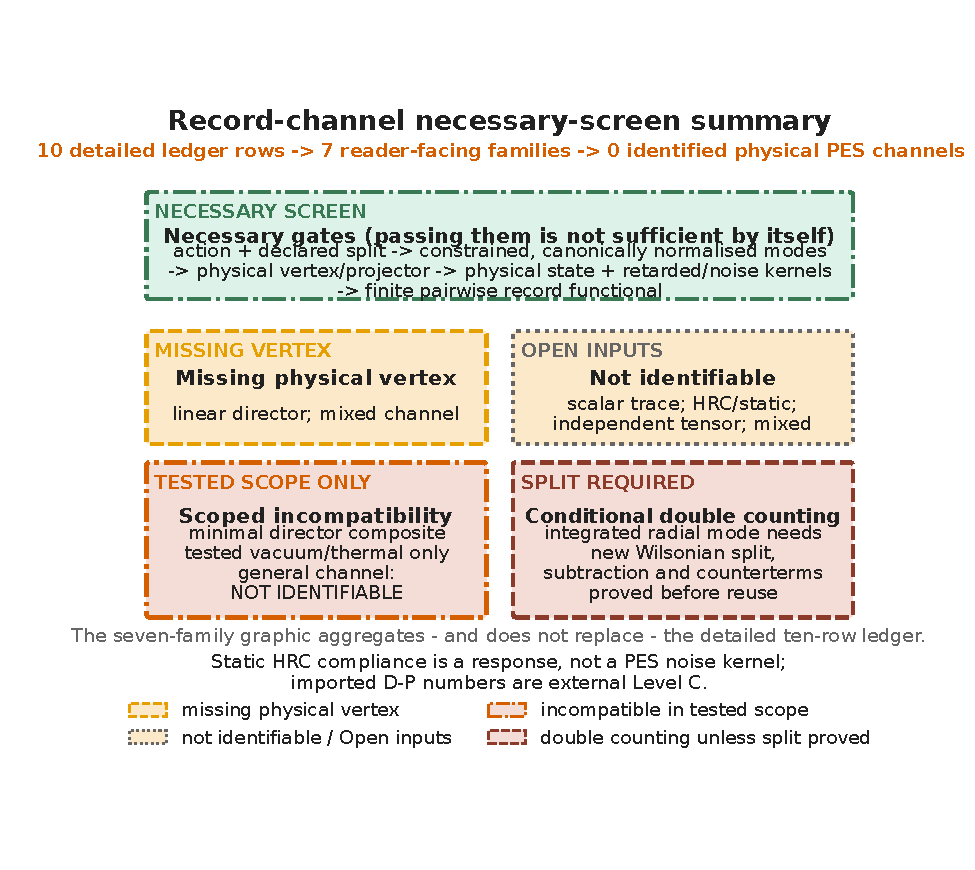
\includegraphics[width=\textwidth]{figures/r149/r149_mediator_channels_summary_47C.pdf}
\caption{Reader-facing necessary-screen summary of the bounded record-channel
audit.  Seven reader-facing families aggregate the detailed ten-row ledger;
the graphic does not replace that ledger.  None of the tested rows supplies
all necessary ingredients: an action and declared resolved/unresolved split,
constrained and canonically normalised physical modes, a physical
vertex/projector, a state with retarded and noise kernels, and a finite
pairwise record functional.  Passing this screen would be necessary, not by
itself sufficient, for a physical PES channel.  The minimal director
composite is incompatible with a universal Di\'osi--Penrose owner only in
the tested vacuum/thermal channels; the general case remains
\texttt{NOT IDENTIFIABLE}.  Reusing an integrated radial mode is
\texttt{DOUBLE-COUNTED} only unless a new Wilsonian split, subtraction and
counterterm ledger are proved.  Static HRC compliance is a response rather
than a PES noise kernel; the imported Di\'osi--Penrose functional remains
external.  Status colour is redundant with
luminance-separated fill, border/arrow style and explicit terminal text; no
hatch pattern encodes status.  The following native table is the authoritative
ten-row candidate/subcase ledger.}
\label{fig:mediator_channels_terminal_47C}
\end{figure}
\begin{longtable}{@{}L{3.5cm}L{3.2cm}L{3.4cm}L{4.3cm}@{}}
\caption{Authoritative ten-row candidate/subcase ledger for the bounded
mediator-channel audit.}
\label{tab:mediator_channels_terminal_47C}\\
\toprule
Candidate & Vertex/projector & State/noise & Terminal status \\
\midrule
\endfirsthead
\toprule
Candidate & Vertex/projector & State/noise & Terminal status \\
\midrule
\endhead
\bottomrule
\endfoot
Fixed-map linear director & $T^{ww}h_{ww}=0$ & absent & \texttt{MISSING VERTEX} \\
Scalar trace & parametric trace coupling & absent & vertex \texttt{PARAMETRIC ONLY}; channel \texttt{NOT IDENTIFIABLE} \\
Classically trace-free source & absent in minimal scalar model & absent & \texttt{MISSING VERTEX} \\
Finite composite body & charge not closed & absent & \texttt{NOT IDENTIFIABLE} \\
Minimal free scalar vacuum & trace vertex only & vacuum benchmark & \texttt{INCOMPATIBLE} with universal D--P \\
Quadratic director composite & coefficient/projector unclosed & tested minimal vacuum/thermal states & \texttt{INCOMPATIBLE} in tested channels; general case \texttt{NOT IDENTIFIABLE} \\
HRC/static response & static augmented-model response & no bath state & \texttt{NOT IDENTIFIABLE} as PES channel \\
Independent tensor completion & conditional $H_{\mu\nu}T^{\mu\nu}/2$ & ECT state absent & \texttt{NOT IDENTIFIABLE} \\
Integrated radial mode reused as bath & possible trace term & split/\allowbreak subtraction/\allowbreak counterterms absent & \texttt{DOUBLE-}\allowbreak\texttt{COUNTED} only unless a new Wilsonian split, subtraction and counterterm ledger are proved \\
Mixed scalar--orientation & absent & absent & \texttt{MISSING VERTEX / NOT IDENTIFIABLE} \\
\end{longtable}

\subsection{Implications for BMV}
\label{sec:mediator_implications}
No imported collapse-model inversion chooses among these channels.  Closure
requires a nonzero projected two-body vertex, positive state, response and
noise kernels, finite protocol and proof that the reduced map is
nonfactorising where entanglement is claimed.

\paragraph{Open mediator tasks.}
Derive a physical constrained mode bundle and canonical residues; identify the
matter and record operators; specify the state; compute $D^R$ and $N_H$;
declare subtractions; then predict phase, retention and noise for a held-out
protocol.

\paragraph{Static bridge and Wightman diagnostics.}
\label{par:47C-M5-M6-diagnostics}
For this local static diagnostic define
\[
 g=|\nabla\Phi_{\rm gal}|,\qquad x=g/a_M\geq0,\qquad
 Y=x^2,\qquad s=f(Y)=x^2B(x),
\]
where $B$ is the dimensionless local bridge factor.  The variables
$x,Y,s,B$ and
\[
 J_B=\frac{B'_+(0)}{B(0)^{3/2}}
\]
are dimensionless; $g$ and $a_M$ have the same acceleration dimension.
The diagnostic requires $B(0)>0$ and a finite right derivative $B'_+(0)$.
It is undefined if either condition fails or if the limiting derivative is
direction-dependent.  Its stated invariance is restricted to a positive
horizontal acceleration-scale rescaling; it is not a general coordinate,
gauge or environment invariance.  A value such as $J_B=-2$ fixes one local
coefficient, not a unique bridge function, gravitational gauge invariant or
ECT response owner.  In the live static-action pullback a
Jacobian is present, and a two-point static $D^R(0,\mathbf k)$ cannot determine
the first nonlinear bridge coefficient: that requires nonlinear response or
a cubic vertex together with the physical source-to-metric map.  M5 is thus a
convention-declared local research diagnostic, not a record-channel closure
milestone.

Likewise, the admissible M6 consistency test is the pair of physical
Wightman inequalities in Eq.~\eqref{eq:AP6A-Wightman-LMIs}, after the same
projector, operator and filter have been applied to response and noise.  The
arbitrary-matrix absolute-value inequality is false, and complete positivity
alone does not supply a frequency-local kernel theorem.  The current ECT
outcome for either diagnostic remains
\texttt{MISSING VERTEX / MISSING STATE / NOT IDENTIFIABLE}; no positive ECT
claim or numerical rate follows.

\paragraph{P28: primordial record-kernel programme (Open).}
\label{par:P28-primordial-record-programme}
CMB acoustic phase information can constrain a \emph{fully specified}
gauge-invariant primordial reduced channel if that channel predicts a
phase-diffusion law, growing/decaying-mode mixing or isocurvature component
that is propagated through recombination and the Boltzmann transfer map.
Acoustic peaks do not directly measure the pairwise record exponent
$\Phi_{ab}$, the off-diagonal density matrix, state purity or a unique pointer
basis.  Strong dephasing in an amplitude basis can leave the diagonal
two-point power unchanged, while a coherent Gaussian growing-mode seed can
produce acoustic peaks without environment-induced dephasing.

For current ECT the gauge-reduced primordial alternatives, physical record
operator and vertex are missing; the state and generally two-time
nonequilibrium response/noise kernels at the ordering front are missing; and
the curvature-variable, metric, recombination/transfer and likelihood maps
are not identified.  The terminal status is therefore
\texttt{MISSING VERTEX + MISSING STATE/KERNEL + NOT IDENTIFIABLE}.  P28 is a
high-value Open PES--cosmology programme, not a claim that the CMB measures a
$\Phi$-field, a PES pointer or an ECT classicalisation event.

\subsection{Scope and non-claims}
\label{sec:mediator_non_claims}
The taxonomy records terminal outcomes.  It does not promote an untested
candidate to an ECT mediator.

\subsection{Detailed candidate-channel separation}

\paragraph{Why the channels cannot be merged.}
The scalar trace, linear director, quadratic director composite, independent
tensor and mixed candidates have different operators, residues and source
selection rules.  A common long-distance mean force would not make their
noise kernels or quantum channels identical.  Each row of the terminal ledger
must therefore be carried through independently.

\paragraph{Scalar branch.}
The scalar candidate couples parametrically to a trace.  Its finite-body
charge can depend on composition, binding energy and nonlinear screening.
These data must be computed before a two-body phase, lensing response or PES
kernel is assigned.  A scalar channel that merely distinguishes the two path
branches may still be factorising and need not entangle them.

\paragraph{Linear director branch.}
The fixed-map contraction with static density is zero, so this branch stops at
\texttt{MISSING VERTEX}.  A new dynamic-coefficient or nonlocal map would be a
new owner and must be audited from Gate~0 rather than treated as a correction
to the old channel.

\paragraph{Quadratic composite branch.}
The first nonzero director-density candidate may be quadratic in the soft
field.  Such a channel has a two-propagator spectrum and generally non-Gaussian
statistics.  In the verified strict massless Gaussian benchmark the local
spectrum scales homogeneously as
$\omega^4B(c_\chi k/\omega)\Theta(\omega-c_\chi k)$; after spatial convolution
with a smooth translated equal-mass
$|\Delta\rho(\mathbf k)|^2=O(k^2)$ filter, the protocol-integrated record
spectrum scales as $\omega^9$.  With weak second-cumulant coupling, a smooth
UV regulator, and contact subtraction, its oscillatory saturation envelope is
$T^{-8}$.  Together with the thermal $1/k$ regime
$\omega\ll c_\chi k\ll T_b$, this is incompatible with a universal DP kernel
in the tested states.  Other operators, filters, regulators, and states remain
Open, not confirmed.

\paragraph{Independent tensor and mixed branches.}
An independent tensor can provide a standard universal vertex only after its
action and state are derived.  A mixed scalar--orientation branch requires an
explicit operator and constrained Hessian; no such owner is present.  Reusing
a radial or HRC mode already included in the mean action as an unresolved bath
without a Wilsonian split is \texttt{DOUBLE-COUNTED}.

\paragraph{Protocol handoff.}
For any surviving branch, the application file must list the operator, source
projector, state, retarded kernel, Hadamard/noise kernel, finite-time window,
detector coupling and counterterm ledger.  Only then may one compute BMV
phases, decoherence visibility, heating, radiation or force noise.

\section{Topological Sectors, Defect Configurations, and the Dark Sector}
\label{sec:qs_topo_dark}
\label{sec:qs_defects}
\label{sec:qs_dark_sector}
% ==============================================================

\textit{Status: Level~A only for winding and homotopy statements inside
explicitly supplied smooth-phase or target models.  Level~B for a conditional
inventory of nonsmooth or defect-like configurations once a wider
configuration space, action, boundary class and admissibility rules are
supplied.  Open for their existence as physical ECT sectors, their dynamics,
production, stability, interaction cross-sections, abundance and dark-sector
role.
Connection: the smooth coherent branch~BR1, defect-sector material
deferred from ECT Foundations~(\S\ref{sec:defect_sectors}), the
winding/conservation architecture~(\S\ref{sec:qs_conservation}),
the macroscopic dark-sector bridge~(\S\ref{sec:dark_sector}),
vacuum-structure questions~(\S\ref{sec:qs_vacuum_intro}),
exchange-sector topology~(\S\ref{sec:qs_statistics}),
entanglement/common-medium correlations~(\S\ref{sec:qs_entanglement}),
and medium character~(P5).}

\medskip
So far the Quantum Sector has been developed inside the smooth coherent
sector defined by the supplied closure BR1.
This restriction was deliberate: it allowed the phase-sensitive sector
to be constructed cleanly in terms of $\Phi_{\rm eff}=\rho e^{i\theta}$,
winding sectors, loop actions, wave dynamics, canonical structure,
and decoherence.
The present architecture does not establish that the physical ECT
configuration space is wider than this smooth branch.  The subsection instead
records a conditional completion programme for such a wider sector.

\subsection{Defect sectors and their relation to the smooth branch}

\subsubsection*{Why defect sectors are not excluded by BR1}

The smooth coherent-sector rule~BR1 does not state that only smooth
coherent configurations exist. Rather, it identifies the current
constructive branch of the theory as the smooth coherent sector with
well-defined phase and integer winding numbers.
This leaves open whether an owner-complete theory admits a broader space of
configurations outside the smooth branch, including singular cores,
discontinuous ordering data, and nontrivial Euclidean topological transitions.
Such a candidate state space was already flagged in the deferred
defect-sector material~(Section~\ref{sec:defect_sectors}).

The r\^ole of the present subsection is therefore not to abandon BR1,
but to state clearly:
\begin{enumerate}[label=(\roman*)]
  \item which configurations could be admitted outside the smooth coherent
    branch after their action and admissibility rules are supplied;
  \item what would be required for physical relevance;
  \item how a future owner-complete sector could be tested as a dark-sector
    candidate.
\end{enumerate}

\paragraph{Medium reading~(P5).}
Under the medium interpretation~(P5), defect and topological sectors
are not external objects appended to the theory.
They are candidate configurations of a proposed wider ordered-medium
completion; their common physical condensate owner is not derived:
regions where the modulus can vanish, the phase becomes ill-defined,
the ordering data changes discontinuously, or the Euclidean
configuration tunnels between distinct sectors.
The dark-sector question is therefore not ``what extra fundamental
fields must be added?'' but rather ``what wider configurations does the
same ordered medium admit beyond the smooth branch~BR1?''

\paragraph{Connection to winding and conservation architecture.}
The conditional defect inventory developed here is a possible extension of the
winding and conservation structure established in
Section~\ref{sec:qs_conservation}.
In the smooth coherent branch, winding numbers are protected under smooth
deformations on the declared domain.  Thermal suppression of sector changes
does not follow from topology; it additionally needs an action, state and
barrier/rate calculation.  If the wider configuration space is supplied,
defect sectors can contain configurations through which topological protection
fails: vortex cores, discontinuities, and instanton-like transitions are
candidate places where topology can change.
In this sense, Section~\ref{sec:qs_conservation} describes the
protected regime, while the present section describes the wider regime
in which protection can break down.

\subsection{Conditional types of defect and topological configurations}

If an owner-complete wider configuration space is supplied, the main
structurally motivated candidate classes outside the smooth coherent sector
are:

\paragraph{Vortex-core configurations.}
Configurations in which the condensate modulus vanishes on a line or
axis, making the phase $\theta$ ill-defined there.
They are the natural continuation of winding sectors to the regime
where core singularities are allowed or regularised by $\rho\to 0$.

\paragraph{Domain-wall-like configurations.}
Sharp transitions or discontinuities in the ordering data, for example
in orientation variables or in the local branch structure of the
ordered phase.

\paragraph{Instanton-like Euclidean configurations.}
Topologically nontrivial Euclidean saddle configurations that
interpolate between distinct vacuum sectors or coherent sectors.
They lie outside the smooth ordered-sector configurations.  If a
Lorentzian/hyperbolic completion of that sector is supplied, they are not
described by its perturbative coherent branch and are instead natural
candidates for nonperturbative inter-sector transitions.

\paragraph{Composite defect configurations.}
Mixed objects in which phase winding, orientation mismatch, and local
suppression of the order parameter coexist.
At the present stage these should be regarded as plausible
configurations of the wider ordered state space, not yet fully
classified solutions.

\subsubsection*{Status of the defect ontology}

The defect inventory is conditional (Level~B/Open): if an owner-complete
ordered-medium theory admits a phase field together with configurations where
the modulus vanishes or the branch data cease to be smooth, defect-like
sectors can be classified.  P1--P6 and BR1 do not by themselves establish that
physical configuration space or its dynamics.  Core structure, stability,
production channels, interaction cross-sections and relic abundance remain
Open.

\subsection{Dark-sector questions opened by the coherent sector}

\textit{Status: Open programme.  The Level-C HRC algebraic diagnostic, the
late-time background closure, and possible particle, collective, defect, or
topological sectors are separate objects.  No common ECT dark-sector
ontology or dynamical bridge among them has been derived.}

The coherent sector permits candidate smooth excitations and, beyond the
smooth EFT, candidate defect or topological configurations.  Calling either
class ``dark-sector candidates'' is presently a research classification, not
a result that they are stable, produced in the required abundance, weakly
coupled to visible matter, or gravitationally clustered.

The macroscopic galactic calculation supplies a Level-C HRC data diagnostic
with no particle-halo or soft-mode term.  It neither derives that fit from
the condensate nor excludes additional particle or collective components.
Likewise, the late-time background closure does not establish that a
coherent or defect sector is the physical source of dark energy.

For a specified candidate to acquire a quantitative dark-sector status one
must derive its action and spectrum, stability and production history,
couplings to visible matter and gravity, relic abundance, structure-growth
response, and discriminating observables.  Failure of one such completion
would constrain that named completion, not the whole ECT programme.

\subsection{Measurement and observability status}

Three observational levels can be distinguished:
\begin{enumerate}[label=(\roman*)]
  \item \textbf{Macroscopic phenomenology~(MP):}
    modified galactic and cosmological response, already developed in
    detail in Macroscopic Physics;
  \item \textbf{Indirect coherent signatures:}
    conditional relic populations, nonstandard clustering, or
    vacuum-transition effects after an action and production history are
    supplied~(Level~B/Open programme);
  \item \textbf{Direct microscopic detection:}
    currently open and likely model-dependent.
\end{enumerate}
Only the first level is currently developed in substantial detail.

\statussummary
\textit{Established~(Level~A conditional mathematics):}
(i)~integer winding inside the explicitly supplied smooth BR1 closure;
(ii)~the stated homotopy groups of explicitly supplied target spaces and the
corresponding absence or presence of protected map classes inside those
targets.

\textit{Level~B:}
(i)~a conditional inventory of defect sectors after a wider configuration
space, action, boundary class and admissibility rules are supplied;
(ii)~smooth collective excitations as the nearest dark-sector
candidates within separately supplied coherent EFTs;
(iii)~the architectural split of the dark sector into a macroscopic
effective layer and a coherent / topological layer.

\textit{Open:}
(i)~the physical existence and full dynamical classification of defect
sectors in ECT;
(ii)~their production, stability, and interaction mechanisms;
(iii)~a unique first-principles identification of the dominant
dark-sector component;
(iv)~the quantitative r\^ole of defect ensembles in late-time cosmology.

\paragraph{Summary.}
BR1 supplies a smooth coherent-sector closure; it does not prove that this is
the whole physical Quantum Sector or that a wider one exists.  Defect and
nonperturbative sectors beyond the smooth branch form a conditional completion
inventory.  They are conceptually useful candidate components of a
coherent/topological dark-sector programme, not an established ECT ontology.
This preserves the correct division of labour across the article:
macroscopic dark phenomenology is developed in MP, whereas genuinely
topological or defect-based dark ontology belongs to QS.

\subsubsection*{Bridge to black-hole thermodynamics}

The conditional topological and defect inventory developed here records one
possible extension of the Quantum Sector beyond the smooth coherent branch;
it does not complete or establish its physical ontology.
The next section turns to the asymptotic infrared regime of the
same ordered medium. Rather than defect and topological sectors
beyond the smooth branch, it examines the long-wavelength
ordered-branch structure relevant to asymptotic symmetries,
gravitational memory, and soft graviton modes, before the
subsequent transition to the strong-field black-hole sector.

% ============================================================

% ==============================================================
% ==============================================================

% R103:T4 BMS/memory/soft physics retained as external completion targets
\section{Infrared and asymptotic completion targets}
\label{sec:ect_ir_soft}

\textit{Status.  BMS symmetries, gravitational memory and soft-graviton
theorems are established results of asymptotically flat gravity.  Their ECT
ownership is Open because a physical tensor action, asymptotic charges, source,
state and boundary conditions have not been derived.}

\subsection{Restriction to asymptotically flat backgrounds}
\label{sec:ir_restriction}
\paragraph{Restriction.}
Null-infinity statements below apply only to an asymptotically flat completed
metric theory and are not transferred automatically to an FRW background.

\subsection{Why the infrared sector matters}
\label{sec:ir_motivation}
BMS symmetry~\cite{Bondi_vanderBurg_Metzner_1962,Sachs_1962}, memory
\cite{Christodoulou_1991_memory} and soft theorems
\cite{Weinberg_1965_soft,He_Lysov_Mitra_Strominger_2015,Strominger_2018_lectures} are mandatory comparison
targets for any proposed ECT tensor completion.

\subsection{BMS completion gate}
\label{sec:ir_bms}
One must derive the asymptotic phase space, constraints, charges and boundary
conditions of the completed physical metric.  The ordered data
$(\phi_0,n_A^{(0)})$ alone do not imply the BMS group.

\subsection{Memory completion gate}
\label{sec:ir_memory}
Gravitational memory is the standard permanent metric displacement sourced by
radiation.  Calling a persistent $\Delta n_A$ ``memory'' requires a derived map
from $\Delta n_A$ to the physical radiative metric and its source.  That map is
currently \texttt{NOT IDENTIFIABLE}; no ECT memory amplitude is predicted.

\subsection{Soft-graviton completion gate}
\label{sec:ir_soft_gravitons}
Long-wavelength director modes may be soft orientation excitations, but the
fixed-map theorem does not make them helicity-2 soft gravitons.  The latter
require the tensor action, physical projector, asymptotic charges and quantum
state.

\paragraph{Caveat.}
Soft orientation data do not by themselves solve an information problem.

\subsection{Soft-hair comparison}
\label{sec:ir_soft_hair_bridge}
The soft-hair proposal~\cite{Strominger_2018_soft_hair} is retained as an
external comparison.  No ECT soft-hair storage or recovery mechanism follows
before the tensor/asymptotic gates above are closed.

\subsection{Scope and non-claims}
\label{sec:ir_non_claims}
This section defines external IR tests; it derives neither BMS charges, memory,
soft-graviton theorems nor black-hole soft hair from P1--P6.

\subsection{Detailed asymptotic-completion protocol}

\paragraph{Asymptotic data required for BMS.}
The BMS group is defined for a physical asymptotically flat Lorentzian metric
with specified fall-off and gauge conditions at null infinity.  The scalar
characteristic tensor supplies a cone in its own equations but not the
nonlinear metric phase space, Bondi coordinates, symplectic form or surface
charges.  Therefore an ECT BMS statement requires a completed physical metric
and boundary-value problem; residual $O(3)$ symmetry alone is insufficient.

\paragraph{Memory observable.}
Gravitational memory is a persistent change in a gauge-invariant detector
observable produced by the integrated radiative flux.  In a tensor completion
it can be written as a change of asymptotic shear related to hard and soft
charges.  A persistent change $\Delta n_A$ of the condensate orientation is a
different variable.  Establishing a map requires the tensor action, source,
boundary conditions and detector metric.  Without that map no memory
amplitude or sign is predicted.

\paragraph{Soft theorem.}
The leading soft-graviton theorem factorises amplitudes when a physical
massless helicity-2 quantum with universal coupling is added at vanishing
energy.  A long-wavelength gapless director disturbance is not automatically
that particle: under integrability it is longitudinal and its fixed-map TT
projection vanishes.  The soft theorem remains an external target for a
future tensor completion.

\paragraph{Relation among soft theorem, memory and asymptotic symmetry.}
In standard gravity these three descriptions are linked by a common physical
metric phase space and its Ward identities.  ECT may reproduce the triangle
only after it derives the same common owner.  It is inconsistent to import one
corner---for example a long-wavelength mode---and infer the other two without
the charges and radiative symplectic structure.

\paragraph{Soft hair and black holes.}
Soft-hair proposals concern asymptotic charges of a completed gravitational
theory and do not by themselves solve the black-hole information problem.
ECT defect or shell variables may provide additional boundary data, but their
map to BMS charges, their conservation law and their coupling to Hawking
radiation remain Open.  No state-counting or information-recovery conclusion
follows from the orientation analogy alone.

\paragraph{Finite-energy and detector gates.}
An observable prediction must specify a finite-frequency waveform, the
source multipoles, propagation on the completed background, detector response
and the limit connecting it to the asymptotic theorem.  Boundary conditions
must also distinguish a truly asymptotically flat solution from cosmological
or finite-condensate geometries.  These requirements are retained as the
developed IR programme.

\paragraph{Status summary.}
BMS algebra, gravitational memory and soft-graviton factorisation are
standard external Level-A results under their own assumptions.  Their ECT
realisation is Open.  The fixed-map negative theorem rules out the former
linear $\delta n_A$ identification but leaves independent tensor, composite
or nonlocal completions available for future testing.

\section{Black-Hole Thermodynamics, Information Problem, and Holographic-Style Entropy Bounds}
\label{sec:qs_bh}
% backward-compatibility aliases:
\label{sec:qs_black_holes}\label{sec:no_exact_thermality}
\label{sec:critical_shell}
\label{sec:bh_information}
% ==============================================================

\textit{Inputs: coherent-vacuum response
(\S\ref{sec:qs_vacuum_response}), the Unruh-type response
(\S\ref{sec:qs_unruh}), the global/reduced unitarity distinction
(\S\ref{sec:qs_unitarity_status}), the decoherence programme
(\S\ref{sec:qs_decoherence}), the Born-weight route
(\S\ref{sec:qs_born}), the entanglement programme
(\S\ref{sec:qs_entanglement}), and the UV-threshold / singularity
architecture (\S\ref{par:uv_threshold},
\S\ref{par:singularity_programme}).
Aim: to reformulate black-hole thermodynamics within the
ordered-condensate language, explain how apparent thermal mixedness can
arise without fundamental information loss under supplied global
unitarity, and assess a critical ordered-phase shell as a C/Open
strong-field candidate rather than an ECT result.
Status: Level~A only for the generic reduced-state fact that a thermal
marginal can coexist with a pure global state.  Exclusion of fundamental
information destruction in ECT is conditional on a completed globally
unitary interacting strong-field theory and remains Level~B/Open.
Level~C/Open for the critical ordered-phase shell ansatz and for all
constructive horizon-thermodynamic results built on it.
Open for the explicit nonlinear strong-field profile of the shell, the
constructive Page-curve mechanism, and the first-principles derivation
of horizon thermodynamic coefficients from bare~P3~(OP-Q13).
Connection: medium character~(P5), the coherent-vacuum response
programme, the Unruh/horizon continuity, the global/reduced unitarity
distinction, and the branch-breakdown logic of the ordered medium.}

\paragraph{Candidate picture: the horizon as an emergent condensate
interface.}
ECT investigates, but does not derive, a completion in which the
black-hole horizon is represented by an emergent interface in the
condensate medium.
This provides a microscopic language for why semiclassical Hawking
thermality may survive while allowing controlled corrections in
dispersion, late-time correlations, and strong-curvature response.
The present section organises the mechanism and its observable
channels; it does not yet provide a complete first-principles
microtheory of black holes.
The shell model and Page-curve-like behaviour are organisational
candidates.  Absence of fundamental information loss additionally
requires a supplied globally unitary strong-field completion.

\paragraph{What is established, what is closure-dependent, and what
remains open in the black-hole programme.}
\label{par:bh_programme}
The black-hole and information programme in ECT should be read in
three layers.
First, the generic reduced-state identity fixes only that a mixed marginal
can coexist with a pure global state.  ECT has not yet derived the global
strong-field Hilbert space, interacting unitary evolution, physical
subsystem split, or the breakdown trajectory of the ordered branch.
Second, the present article studies a C/Open strong-field candidate:
the near-horizon critical shell.
Within that closure, approximate horizon thermality, enlarged-state
bookkeeping and reduced-state mixedness can be organised consistently.
Preservation of the global information requires the additional hypothesis
of a unitary interacting completion; it is not supplied by the shell ansatz.
Third, what remains open is the completed nonlinear evaporation
problem: the exact shell dynamics, the precise Page-curve mechanism,
and the fully explicit bridge between the reduced thermal appearance
and the globally unitary condensate evolution.

\medskip
A consistent Quantum Sector cannot stop at wave dynamics, commutators,
decoherence, and Born-type probabilities.
It must also address the strongest known tension between quantum
unitarity and horizon thermodynamics: the black-hole information
problem.
The corresponding accelerated-observer version of the same
vacuum-response logic is developed earlier in
Section~\ref{sec:qs_unruh}.
The purpose of the present subsection is twofold:
\begin{enumerate}[label=(\roman*)]
  \item to reformulate black-hole thermodynamics within the
    ordered-condensate language of ECT;
  \item to show that apparent thermal mixedness is compatible with global
    purity, while keeping global ECT unitarity as an explicit Open owner.
\end{enumerate}

\paragraph{Medium reading~(P5).}
Under P5, a future strong-field completion may represent the
black-hole horizon as an interface of an ordered condensate rather than
as a primitive boundary.  The present action has not derived that
interface or its weak-to-strong-field metric map.
The information problem is therefore reformulated in medium language:
not ``does spacetime destroy information?'', but ``how does one
ordered condensate reorganise accessible and inaccessible coherent
sectors in the strong-field regime?''
Apparent thermality, reduced-state mixedness, and limited observer
access are all properties of one physical medium rather than of a
separate ontological stage.

\paragraph{Connection to the Unruh/horizon continuity.}
The black-hole programme asks whether a future strong-field completion
can connect to the standard Unruh/Rindler target of
Section~\ref{sec:qs_unruh}.  Neither a common ECT response operator nor
a physical shell is presently derived.  A Tolman temperature may be
used as an input in the shell toy model, but it does not dynamically
create or select that shell from P1--P6.

\paragraph{Discriminant with respect to standard black-hole
resolutions.}
ECT investigates a completion in which global information is preserved,
but this is a conditional programme rather than a consequence of P1--P6.
It also does not solve the problem by simply postulating a bounce,
a remnant, or a new microscopic interior law unrelated to the rest of
the theory.
Instead, it uses the same ordered medium, the same reduced-state
logic, and the same branch structure already employed in decoherence,
vacuum response, and singularity breakdown.
The proposed closure reads apparent thermality as a reduced-state
phenomenon and tests whether a condensate branch reorganisation can carry
the missing correlations.  Both the branch reorganisation and global
unitarity remain to be constructed.

\subsection{Effective horizon thermodynamics}
\label{sec:bh_eff_thermo}

\subsubsection*{Black-hole thermodynamics as the effective horizon response}

At the effective macroscopic level, a black hole is characterised by
its horizon area $A_H$ and surface gravity $\kappa_H$.
In standard semiclassical language (using the conventional $\hbar$
before the $S_0=\hbar$ identification):
\pagebreak[3]
\begin{equation}
  \label{eq:qs_Hawking_temp}
  T_H
  =
  \frac{\hbar\,\kappa_H}{2\pi c\,k_B},
\end{equation}
\begin{equation}
  \label{eq:qs_BH_entropy}
  S_{BH}
  =
  \frac{k_B\,A_H c^3}{4G_N\hbar}.
\end{equation}
Within ECT these formulas are the effective thermodynamic target that
the coherent branch must reproduce or reinterpret; they are
not claimed as first-principles derivations from bare~P3.

Once the identification~\eqref{eq:qs_S0_identification} is completed,
they can be written in the equivalent ECT form
\begin{equation}
  \label{eq:qs_Hawking_temp_S0}
  T_H
  =
  \frac{S_0\,\kappa_H}{2\pi c\,k_B},
  \qquad
  S_{BH}
  =
  \frac{k_B\,A_H c^3}{4G_N S_0}
\end{equation}
This rewriting is Level~B since it depends on the final
$S_0=\hbar$ identification~\eqref{eq:qs_S0_identification}.

\subsubsection*{First law and generalized entropy bookkeeping}

At the effective thermodynamic level, the horizon sector should also
satisfy the first-law structure
\begin{equation}
  \label{eq:qs_BH_first_law}
  dM = T_H\,dS_{BH} + \Omega_H\,dJ + \Phi_H\,dQ,
\end{equation}
where the angular-momentum and charge terms are included for generality.
Within ECT this equation is an external effective consistency target,
not a first-principles derivation from bare~P3.
Equation~\eqref{eq:qs_BH_first_law} should therefore be read as a
Open effective thermodynamic target for the completed strong-field
closure, not yet as a first-principles derivation from bare~P3.

The important conceptual point is the entropy bookkeeping.
The relevant entropy for the information problem is not the horizon
entropy alone, but the \emph{generalized} coarse-grained entropy of the
external description:
\begin{equation}
  \label{eq:qs_generalized_entropy}
  S_{\rm gen}
  = S_{BH} + S_{\rm ext}^{\rm coarse},
\end{equation}
where $S_{\rm ext}^{\rm coarse}$ is the coarse-grained entropy of the
outside radiation sector.
This is standard generalized-entropy bookkeeping after a subsystem
split is supplied.  ECT has not yet derived the required Hilbert-space
factorisation or observer algebra.

Thus the correct thermodynamic question is not whether $S_{BH}$ alone
changes, but whether the external coarse-grained description evolves
consistently once horizon, shell, and radiation sectors are treated
together.

\paragraph{Status.}
Equation~\eqref{eq:qs_BH_first_law} is an external effective target.
Equation~\eqref{eq:qs_generalized_entropy} is supplied semiclassical
bookkeeping, with its physical ECT owner Open.
Its exact dynamical evolution in the completed evaporation problem
remains open~(OP-Q13).

\subsection{The information paradox in ECT}
\label{sec:bh_info_paradox}

\subsubsection*{The paradox in brief}

The information paradox arises from three apparently simultaneous
ingredients:
\begin{enumerate}[label=(\roman*)]
  \item pure-state gravitational collapse,
  \item thermal Hawking emission,
  \item complete evaporation of the hole.
\end{enumerate}
If the outgoing radiation is exactly thermal and the hole disappears
completely, the final state appears mixed even when the initial state
was pure.
Schematically,
\begin{equation}
  \label{eq:qs_info_loss_naive}
  |\Psi_{\rm in}\rangle\langle\Psi_{\rm in}|
  \;\longrightarrow\;
  \rho_{\rm rad}^{\rm thermal},
\end{equation}
which would violate unitarity if taken as the \emph{fundamental}
evolution law of the full system.

\subsubsection*{ECT reformulation of the paradox}

ECT changes the conceptual framing.
The relevant question is not: \emph{does spacetime itself destroy
information at the horizon?}
The correct question inside ECT is: \emph{how does the ordered
condensate reorganise the distinction between accessible and
inaccessible coherent sectors near a strong-field horizon?}

In a supplied globally pure coherent completion, mixedness may arise after
coarse-graining or a partial trace.  This is one consistent reading of
Hawking thermality, not a proof that fundamental state destruction is
excluded by the present ECT action.

\subsubsection*{Ontological status of the paradox in ECT}

Before specifying the critical-shell mechanism, it is useful to state
what the information-paradox question becomes once the primitive
ontology of ECT is used consistently. In its sharpest semiclassical
form the paradox relies on three assumptions that are usually left
implicit:
\begin{enumerate}[label=(\roman*)]
  \item Lorentzian spacetime is the fundamental arena;
  \item the horizon is a fundamental geometric locus rather than an
        emergent effective boundary;
  \item the inside/outside split defines an observer-independent
        decomposition of the fundamental degrees of freedom.
\end{enumerate}

ECT does not treat these assumptions as primitive. The primitive
object is the four-dimensional Euclidean condensate field $\Phi$.
Lorentzian spacetime, causal cones, horizons, and the inside/outside
distinction belong to the ordered-branch effective description. This
does not make them unreal or arbitrary: within the Lorentzian branch
they are physically meaningful and operationally measurable. But
their status is emergent and reduced, not fundamental.

This changes the bookkeeping but not the unitarity question.  The fact that
a horizon is emergent does not logically exclude non-unitary microscopic
dynamics.  It motivates treating the horizon as a boundary in a reduced
ordered-branch description. The candidate split is
therefore not between ``fundamental inside'' and ``fundamental
outside'', but between the full coherent/reconstructed condensate
description and the exterior reduced state,
\[
  \rho_{\rm ext}
  =
  \mathrm{Tr}_{\rm shell,int}\,
  |\Psi\rangle\langle\Psi|,
\]
or its appropriate reconstructed/coarse-grained analogue.

Three consequences follow.

\paragraph{First.} Hawking thermality is naturally interpreted as
reduced-state thermality. A thermal exterior density matrix does not
by itself imply fundamental non-unitary evolution, just as a
thermalised subsystem in ordinary quantum theory does not imply loss
of the global state.

\paragraph{Second.} The question ``is information destroyed?'' splits
into two distinct questions: whether a globally unitary ECT completion
exists, and whether observer-accessible asymptotic radiation recovers its
correlations.  Both depend on the completed strong-field dynamics; the
second is the constructive Page-curve problem~(OP-Q13).

\paragraph{Third.} The critical-shell model is one possible C/Open
completion to test.  The present theory does not show that the ordered
branch fails at a shell, that a pre-Lorentzian interior takes over, or
that such a shell mediates between them.

\paragraph{Status.} The generic conditional statement is that a
globally unitary completed strong-field theory preserves global
information by assumption.  That premise is not supplied by P2 and
remains Open.  The constructive recovery of correlations in the
exterior radiation, including a quantitative Page curve, remains Open.
The critical ordered-phase shell is only one optional C/Open
completion, not the owner of that problem.

\subsubsection*{The critical ordered-phase shell}

One C/Open candidate is a strong-field transition region near the
horizon, where the ordered Lorentzian branch becomes critically
strained.  In the supplied ansatz this is described as a
\emph{critical ordered-phase shell}: a finite region surrounding the
effective horizon in which:
\begin{enumerate}[label=(\roman*)]
  \item the macroscopic Lorentzian ordering becomes marginal,
  \item coherent and topological degrees of freedom become strongly
    coupled,
  \item the outside observer's effective Hilbert-space description
    ceases to coincide with the full condensate state space.
\end{enumerate}
This shell is a Level~C/Open strong-field ansatz, not a result of
bare~P3.  Its existence, location, stability, state space and coupling
to radiation are all missing owners.

\subsubsection*{Enlarged Hilbert space and apparent mixedness}

The key structural point is that the external observer does not have
access to the full condensate state space.
For a supplied shell toy model one may posit the decomposition
\begin{equation}
  \label{eq:qs_H_total}
  \mathcal{H}_{\rm total}
  =
  \mathcal{H}_{\rm ext}
  \otimes
  \mathcal{H}_{\rm shell}
  \otimes
  \mathcal{H}_{\rm int},
\end{equation}
where $\mathcal{H}_{\rm ext}$ is the asymptotically accessible exterior
sector, $\mathcal{H}_{\rm shell}$ is the critical ordered-phase shell
sector, and $\mathcal{H}_{\rm int}$ is the interior or otherwise
inaccessible strong-field sector.
The decomposition~\eqref{eq:qs_H_total} is Level~C/Open: no physical
ECT Hilbert space, tensor product, subsystem algebra or shell factor is
derived from bare~P3.

\begin{figure}[tbp]
\centering
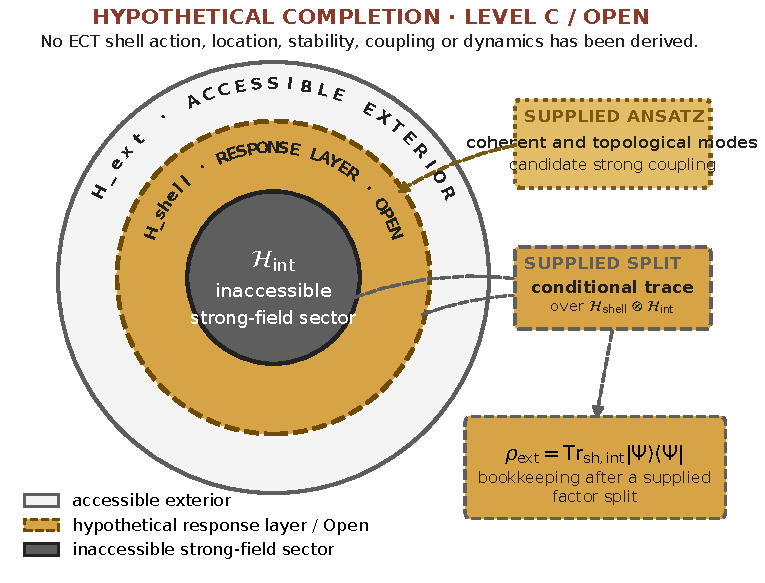
\includegraphics[width=0.92\textwidth]{figures/r155/fig_bh_shell_r155.pdf}
\caption{Level-C/Open schematic of a hypothetical near-horizon response
layer.  Curved labels follow the concentric regions: an accessible exterior,
a hypothetical response layer, and an inaccessible strong-field sector.  The
amber callout marks the supplied ansatz that coherent and topological modes
become strongly coupled in the shell.  Two gray leader lines identify the
shell and interior sectors as supplied factors of a conditional trace; they
are not dynamical arrows.  The sole gray arrow runs from that trace operation
to the reduced exterior state $\rho_{\rm ext}$.  This bookkeeping requires a
separately supplied Hilbert-factor split.  No ECT shell action, location, stability,
coupling, subsystem factorisation or dynamics is derived by this picture, and
it is not a completed global solution of the evaporating black-hole problem.}
\label{fig:qs_bh_shell}
\end{figure}

Figure~\ref{fig:qs_bh_shell} is schematic: it visualises the current
Level~C/Open ansatz and should not be read as a solved global
metric profile.
For the present strong-field bookkeeping, generalized-entropy structure,
and the open shell-dynamics problem, see
Appendices~\ref{app:bh_info}, \ref{app:conditional_theorem},
and~\ref{app:chi_dynamics}.

The physically observed radiation state is not the total state but
a reduced state:
\begin{equation}
  \label{eq:qs_rho_ext}
  \rho_{\rm ext}
  =
  \mathrm{Tr}_{{\rm shell,int}}
  \bigl(|\Psi_{\rm total}\rangle\langle\Psi_{\rm total}|\bigr).
\end{equation}
A reduced state of this form can be approximately thermal when the
tensor-product split, pure total state and unitary evolution are all
supplied.  None of those black-hole owners follows from the shell
ansatz itself.
\FloatBarrier

\subsubsection*{Page-curve logic in ECT language}

A useful way to formulate the information problem operationally is through
the Page-curve question: does the entropy of the outgoing radiation
continue to rise until the end of evaporation, or does it eventually turn
over under a supplied complete-evaporation, no-remnant unitary channel with
a physical time-dependent factorisation and final-radiation subsystem?

In ECT the sharpest current statement is structural.
If the total ordered-condensate evolution remains unitary on
$\mathcal{H}_{\rm total}$~\eqref{eq:qs_H_total}, then the radiation
entropy seen by the external observer is the entanglement entropy of a
reduced sector, not a fundamental entropy of the full state.
Therefore a Page-like turnover is not forbidden in principle, but it is not
selected by unitarity or subsystem bookkeeping alone
(see~\eqref{eq:qs_generalized_entropy}).

What is still missing is the explicit strong-field evolution law needed to
compute a concrete Page curve from the ECT shell dynamics:
\begin{itemize}
  \item a Page-compatible evolution is mathematically possible under a
    supplied globally unitary completion;
  \item the \emph{explicit Page curve} is still open~(OP-Q13).
\end{itemize}

\paragraph{Summary.}
The reduced-state formulation changes the logic of the Page problem: the
radiation entropy is that of an observer sector, so apparent thermality does
not by itself prove destruction of full-state information.  It also does not
prove that a globally pure interacting ECT completion exists.

\subsubsection*{Conditional reduced-state compatibility}

The quantum-sector bookkeeping records the generic facts
(Sections~\ref{sec:qs_decoherence} and~\ref{sec:qs_born}) that:
\begin{enumerate}[label=(\roman*)]
  \item coherent amplitudes are primary;
  \item mixedness emerges from reduction or decoherence;
  \item reduced observers need not track the full coherent
    state space.
\end{enumerate}
These facts do not weaken or solve the black-hole paradox on their own.
The same reduced-state logic can be applied to a horizon only after a
physical Hilbert-space factorisation and global dynamics are supplied.
Observer-dependent mixedness is then a possible interpretation, not a
default forced by P1--P6.

\subsubsection*{Conditional theorem: thermality without fundamental information loss}

The strongest honest statement currently available is the following
conditional result.

\begin{quote}
\textbf{Conditional reduced-state identity.}
If a tensor-product split, globally pure state and global unitary
evolution are supplied, then an approximately thermal reduced state
$\rho_{\rm ext}$~\eqref{eq:qs_rho_ext} is compatible with preservation
of the global state.  This statement is generic quantum mechanics and
does not derive a critical shell, Hawking spectrum, evaporation channel
or Page curve.
\end{quote}

Status:
\begin{itemize}
  \item \textbf{Level~A}: the general logic that thermal reduced states
    do not imply fundamental nonunitary evolution is a structural
    consequence of the global/reduced unitarity distinction together
    with the reduced-state formalism established in
    Sections~\ref{sec:qs_unitarity_status},
    \ref{sec:qs_decoherence}, and~\ref{sec:qs_born}.
  \item \textbf{Level~C/Open}: the critical ordered-phase shell ansatz;
    its physical state, vertex and dynamics are not derived.
\end{itemize}

\subsubsection*{Conditional reduced-state reframing}

The black-hole information problem depends on a specific set of premises,
including semiclassical exterior dynamics in its stated regime, a physical
subsystem/algebra split, the evaporation channel, and a global information
law.  Declaring the Lorentzian metric emergent does not by itself remove or
weaken the conflict.  A completed ECT model would have to derive which
premise is modified and then demonstrate a globally consistent evolution
and the observable radiation channel.  The present coherent/critical-shell
picture supplies neither result and is therefore an Open strong-field
programme, not a resolution.

\subsection{Comparative mapping: a candidate shell and the islands/QES language}
\label{sec:bh_islands_comparative}

\textit{Status: Level~C/Open analogy. The islands formula
and the QES formalism are standard tools of the modern
semiclassical/holographic black-hole programme. The present
subsection translates the candidate ECT critical-shell picture of
Section~\ref{sec:bh_info_paradox} into that language, without
claiming a derivation of either framework from the other.
Connection: the Hilbert-space decomposition~\eqref{eq:qs_H_total};
the reduced-state reading of Hawking thermality; the global/reduced
unitarity distinction~(\S\ref{sec:qs_unitarity_status}); the
IR/soft-hair bridge of
Section~\ref{sec:ir_soft_hair_bridge}.}

\subsubsection*{Why a mapping is useful}

Section~\ref{sec:bh_info_paradox} formulated the ECT reading of
Hawking thermality through a critical ordered-phase shell and the
Hilbert-space decomposition
$\mathcal{H}_{\rm total}=\mathcal{H}_{\rm ext}\otimes\mathcal{H}_{\rm shell}\otimes\mathcal{H}_{\rm int}$
in~\eqref{eq:qs_H_total}. The modern holographic programme arrives
at Page-curve-compatible radiation dynamics through a different
language: that of quantum extremal surfaces and islands. The
present subsection maps the two languages onto each other as far as
current structure allows. \emph{The point of the present mapping is
compatibility of structural logic, not an ECT derivation of the
Page curve.} Both pictures distinguish between globally unitary
bookkeeping and the reduced thermal entropy seen by an exterior
observer; that common logic is what makes the mapping possible.

\subsubsection*{Brief recap of the QES/islands programme}

The modern holographic programme computes the entropy of Hawking
radiation via the generalised
entropy~\cite{Ryu_Takayanagi_2006,Faulkner_Lewkowycz_Maldacena_2013}
\begin{equation}
\label{eq:Sgen_recap}
S_{\rm gen}(\Sigma) = \frac{\mathrm{Area}(\partial\Sigma)}{4\,G_N} + S_{\rm bulk}(\Sigma),
\end{equation}
extremised over bulk regions $\Sigma$~\cite{Engelhardt_Wall_2015}.
The inclusion of disconnected ``island'' regions
inside the black hole proves decisive for radiation
entropy~\cite{Penington2020,Almheiri_Engelhardt_Marolf_Maxfield_2020}:
before the Page time the minimal QES is empty; after the Page time
a non-trivial island dominates, yielding the Page-curve turnover.

\subsubsection*{Core structural mapping}

Table~\ref{tab:bh_islands_mapping} sets out the structural
correspondence between the two languages.

\renewcommand{\arraystretch}{1.3}
\begin{longtable}{@{}L{5.0cm}L{4.4cm}L{5.7cm}@{}}
\caption{Structural mapping between the ECT critical-shell picture
and the QES/islands language. Entries in the right column are
structural analogies, not derived equivalences.}
\label{tab:bh_islands_mapping}\\
\toprule
ECT side & Islands/QES side & Structural relation \\
\midrule
\endfirsthead
\toprule
ECT side & Islands/QES side & Structural relation \\
\midrule
\endhead
\bottomrule
\endfoot
$\mathcal{H}_{\rm int}$ (interior / inaccessible sector)
 & island region
 & structurally analogous role: degrees of freedom outside the exterior reduced description but counted in the globally unitary picture \\
boundary of critical ordered-phase shell
 & quantum extremal surface boundary $\partial\Sigma$
 & structurally analogous interface between accessible and inaccessible sectors \\
$\rho_{\rm ext}=\mathrm{Tr}_{\rm shell,int}|\Psi_{\rm total}\rangle\langle\Psi_{\rm total}|$
 & reduced radiation state whose entropy is given by $S_{\rm gen}$ at the dominant QES
 & both are reduced-state objects only after global unitarity and subsystem algebras are supplied \\
Page-curve possibility under supplied global isometry and factorisation
 & Page-curve turnover via island transition
 & qualitative Page-curve compatibility, not a derivation \\
long-wavelength $\delta n_A$ modes near the critical shell
 & soft hair on or near the horizon
 & candidate long-wavelength bookkeeping sector, independently formulated \\
\end{longtable}

\subsubsection*{Where the mapping is formal and where it is structural only}

\paragraph{Formal identity and proposed analogy.}
The generic identity that a mixed reduced state may arise from a pure global
state is common mathematical bookkeeping.  No further equivalence has been
derived.  The proposed correspondence between an island/interior algebra and
the supplied ECT $\mathcal{H}_{\rm int}$ label, or between a shell boundary
and $\partial\Sigma$, is an Open analogy until the ECT subsystem algebras,
entropy functional and extremisation rule are constructed.

\paragraph{Structural only.}
ECT does not derive the generalised entropy
formula~\eqref{eq:Sgen_recap} from first principles. The
critical-shell / Hilbert-space decomposition is compatible with
such a formula but does not imply it. ECT also does not provide a
replica-wormhole-type computation; replica wormholes are a
Euclidean gravitational path-integral device, and an analogous
computation on the underlying Euclidean condensate path integral is
an open item. The detailed time dependence of the ECT Page curve
requires the explicit shell dynamics flagged as OP-Q13 in
Section~\ref{sec:bh_info_paradox}.

\paragraph{Shell is not a derived QES.}
In particular, the critical-shell boundary is not here identified
with a derived quantum extremal surface. At present it is only a
structurally analogous interface separating reduced exterior
thermality from the globally unitary description.

\subsubsection*{Scope and non-claims}

The present subsection does not claim
(i) a first-principles derivation of the QES or islands formula
from ECT;
(ii) a replica-wormhole-type calculation in ECT;
(iii) an explicit Page curve for a specific ECT evaporation
scenario;
(iv) that the critical-shell picture and the islands picture are
formally equivalent.
Its claim is narrower: the generic reduced-state identity is compatible
with either bookkeeping scheme under separately supplied assumptions.
No structural alignment, Page curve or common physical mechanism is inferred.

% ==============================================================
\subsection{Black-hole entropy and observational signatures}
\label{sec:bh_entropy_obs}

\subsubsection*{Black-hole entropy in the ECT reading}

In a supplied semiclassical black-hole model, $S_{BH}$ is the standard
Bekenstein--Hawking entropy.  A future ECT completion might seek to represent
it through a coarse-grained external description, but the required
subsystem algebra, state, area coefficient and strong-field action have not
been derived.  The generic fact that reduced descriptions can be mixed does
not identify $S_{BH}$ with condensate entropy.

\subsubsection*{Relation to Hawking radiation and vacuum effects}

ECT does not deny Hawking-like emission.
Sections~\ref{sec:qs_particle_production} and~\ref{sec:qs_unruh}
record standard conditional targets; they do not derive
horizon-induced excitation production from ECT.  A reduced-state
interpretation is compatible with a supplied globally pure completion,
not forced by the present action.

\subsubsection*{Thermality versus exact thermality}

The black-hole information problem becomes most severe if the outgoing
radiation is assumed to be \emph{exactly} thermal at all stages.
ECT does not require such exact thermality.
The shell ansatz does not itself derive approximate thermality of the
reduced external state~\eqref{eq:qs_rho_ext}; that property must come
from a supplied or derived evaporation channel.

This distinction matters.
Approximate thermality is perfectly compatible with hidden correlations,
late-time purification effects, and a Page-curve turnover.
Exact thermality would be much harder to reconcile with global unitarity.

The correct conditional statement is: a thermal marginal can coexist
with a pure global state when the physical factorisation and global
isometry are supplied.
This shows how a future unitary ECT completion could avoid the strongest
form of the paradox, but neither that completion nor the quantitative
evaporation problem has been derived~(OP-Q13).

\subsubsection*{Missing strong-field forward model}

No ECT strong-field observable follows from the shell label alone.  A
completion must first supply a physical action and state, a regular
strong-field solution, matter/photon/tensor perturbation operators with
boundary conditions, a source/detector vertex, a causal radiation channel,
and an observable likelihood.  Standard Hawking and exterior-metric results
are external targets until that owner chain is complete.

\paragraph{No retained phenomenological response ansatz.}
No near-horizon dispersion law or energy-dependent gravitational response
is derived from P1--P7.  Arbitrary functions for those effects would
parameterise generic deviations rather than ECT and are not retained.

\paragraph{Observable status.}
ECT currently predicts no nonzero ringdown shift, echo, reflectivity,
primordial-black-hole correction or other shell signature.  Future data can
test only a completed model that derives one of these observables together
with its nuisance and likelihood structure.

\paragraph{What ECT does not yet provide.}
ECT does not yet provide a full Level~A dynamical solution of the
black-hole information problem.
The positive mechanism---how approximate horizon thermality,
shell/interface dynamics, and global purity are jointly
realised---remains to be constructed.

\paragraph{What is established and what remains conditional.}
The exact statement is the generic reduced-state identity: thermal
marginals do not imply destruction of information if the global state
evolves unitarily.  ECT has verified this logic in reconstructed
positive Gaussian subsectors.  Applying it to an evaporating black hole
requires a completed interacting Hilbert space, global unitary dynamics,
strong-field metric/vertices and a physical subsystem factorisation;
these are not consequences of P2 and remain B/Open.  The relevant
status distinction is developed in
Sections~\ref{sec:qs_unitarity_status},
\ref{sec:qs_decoherence}, and~\ref{sec:qs_born}:
reduced-state thermality does not imply fundamental loss of
information \emph{when} the total evolution remains globally unitary.

\statussummary
\textit{Established~(Level~A, conditional-domain mathematics):}
(i)~a thermal reduced state can be compatible with global purity;
(ii)~positive Gaussian subsectors admit the standard reconstructed
unitary description under the named OS hypotheses.

\textit{Level~C/Open shell ansatz:}
the critical shell, enlarged Hilbert-space bookkeeping, approximate
Hawking channel, Page-like toy and branch-boundary interior picture.
Global interacting unitarity and all physical subsystem/state owners
remain Open.

\textit{Open~(OP-Q13):}
(i)~the explicit nonlinear strong-field profile of the critical shell;
(ii)~the constructive Page-curve mechanism;
(iii)~the first-principles derivation of horizon thermodynamic
coefficients from bare~P3;
(iv)~the completed strong-field evaporation dynamics.

In particular, the present shell analysis does not yet derive the full
interior profile, first-principles horizon thermodynamic coefficients,
or a constructive Page curve; the numerical coefficient in the
area-law entropy $S_{\rm shell}\sim A/\ell_*^2$ remains an open
matching condition.

% ==============================================================
\subsection{Conditional boundary-cell counting and the open
area-law programme}
\label{sec:area_law}
% ==============================================================

\textit{Status: Level~A mathematics only for the conditional
finite-cell counting lemma below, after a subsystem split,
coarse-graining, finite local entropy capacity, and an area-law
state class have all been supplied.  ECT ownership of those inputs,
the ultraviolet completion, the black-hole coefficient, and the
physical entropy bound is Open.
Connection: shell entropy~(\S\ref{app:shell_entropy}),
conditional theorem~(\S\ref{app:conditional_theorem}),
decoherence programme~(\S\ref{sec:qs_decoherence}),
entanglement~(\S\ref{sec:qs_entanglement}),
EFT breakdown scale~(\S\ref{par:uv_threshold}),
medium character~(P5).}

\subsubsection*{Problem statement: area law, holographic bound, and
full holography}

In black-hole physics, entropy scales with area rather than volume.
In the broader quantum-gravity literature this motivates several
related but conceptually distinct ideas:
\begin{enumerate}[label=(\roman*)]
  \item the Bekenstein--Hawking area law for black-hole
    entropy~\cite{Bekenstein1973};
  \item more general holographic-style entropy
    bounds~\cite{Bekenstein1981,tHooft1993,Susskind1995};
  \item the stronger holographic principle in the sense of bulk
    encoding or reconstruction by boundary
    data~\cite{Bousso2002}.
\end{enumerate}
These statements should not be conflated.
An area law does not by itself imply full holography, and a
shell-counting argument near horizons does not by itself establish
a covariant entropy bound for arbitrary dynamical geometries.

The ECT question is narrower than an assertion of holography:

\emph{Which additional microscopic and state assumptions would make
an area-type entropy count compatible with the local ordered-medium
picture, and which of those assumptions are actually derived?}

The answer presently available is conditional.  Locality and a mass
gap motivate an interfacial description of low-energy correlations,
but they do not by themselves regulate continuum entanglement or
prove an area law for an arbitrary state.

\subsubsection*{Necessary distinctions}

Three scales and statements must be kept separate.
\begin{enumerate}[label=(\roman*)]
  \item The homogeneous P3 mass
    $m_{\Phi,\mathrm{rad}}$ defines a P3 Gaussian infrared correlation
    length $\xi_{\rm P3}=m_{\Phi,\mathrm{rad}}^{-1}$.  It does not define a
    P4 or gravitational EFT breakdown scale.
    A massive continuum field nevertheless contains modes of
    arbitrarily large wave number within the formal continuum theory.
    Therefore $m_\sigma^{-1}$ is not, without a microscopic
    completion, a lattice spacing, a hard ultraviolet regulator, or a
    finite-dimensional local Hilbert-space cell.
  \item Exponential decay of selected two-point functions does not
    imply that all bipartite entropy is confined to a boundary layer.
    Arbitrary states of a local system may have volume-law or
    data-hiding entanglement despite short-ranged two-point
    correlations.
  \item A finite area count follows only after a physical split and a
    state class with an area-law property are specified together with
    a finite coarse-grained local capacity.  Those inputs are not
    consequences of P1--P6 at present.
\end{enumerate}

\subsubsection*{Conditional setup}

Let $\Sigma$ be a smooth closed two-surface separating exterior
and interior subsystems.
The reduced state of the exterior observer is
\begin{equation}
  \label{eq:rho_ext_area}
  \rho_{\rm ext}
  = \mathrm{Tr}_{\rm int}\,|\Psi\rangle\langle\Psi|,
  \qquad
  S_{\rm red}(\Sigma)
  = -\mathrm{Tr}(\rho_{\rm ext}\ln\rho_{\rm ext}).
\end{equation}
Equation~\eqref{eq:rho_ext_area} itself requires a supplied
factorisation (or an appropriate algebraic split).  Gauge and
constrained sectors may require edge modes and need not admit the
naive tensor-product factorisation.

\paragraph{Supporting lemma (exponential clustering).}
For the supplied homogeneous P3 Gaussian sector, with
$m_\sigma\equiv m_{\Phi,\mathrm{rad}}>0$, the connected two-point
correlator satisfies
$|\langle\Phi(x)\Phi(y)\rangle_c|
\le C\,e^{-m_{\Phi,\mathrm{rad}}|x-y|}$
(standard result for massive Euclidean
fields~\cite{GlimmJaffe1987}).
Its cross-boundary \emph{two-point} correlations are therefore
exponentially suppressed over
$\xi_{\rm P3}=O(m_{\Phi,\mathrm{rad}}^{-1})$.  This is useful
long-distance information inside that supplied sector, but it is neither a
P4 pole nor a UV regulator or entropy-area theorem.

\paragraph{Supplied coarse-grained inputs.}
Let $\ell_{\rm cg}$ be an explicitly chosen physical lattice spacing,
UV cutoff, or coarse-graining resolution; let $s_{\rm cg}<\infty$ be
the maximum entropy assigned to one retained cell under a declared
finite-dimensional truncation or energy restriction.  Neither
$\ell_{\rm cg}$ nor $s_{\rm cg}$ is currently derived from
$m_\sigma$ or from P1--P6.

In addition, assume a state class for which the cross-interface
entropy is supported, up to a declared remainder $\Delta S$, in a
layer of thickness $\xi_{\rm ent}$.  Examples of sufficient inputs
would be a finite-depth local preparation from a product state, an
appropriate quantum-Markov/conditional-mutual-information bound, or
an independently proved area law for the selected gapped state.
Finite correlation length alone is not substituted for this
assumption.

\subsubsection*{General theorem}

\begin{theorem}[Conditional boundary-cell counting lemma]
\label{thm:area_bound}
Let $\Sigma$ be a smooth closed two-surface of area $A(\Sigma)$
separating supplied interior and exterior subsystem algebras.  Suppose
that:
\begin{enumerate}[label=\textup{(\roman*)}]
  \item a lattice, UV completion, or coarse-graining of resolution
    $\ell_{\rm cg}$ is supplied;
  \item each retained cell has entropy capacity at most
    $s_{\rm cg}<\infty$ under the stated truncation or energy bound;
  \item the selected state class obeys a boundary-localisation
    hypothesis: all but a remainder $\Delta S$ of the entropy across
    the split is carried by cells within distance $\xi_{\rm ent}$ of
    $\Sigma$;
  \item the geometry is regular on those scales, so the number of
    cells in that layer is bounded by
    $C_\Sigma A(\Sigma)\xi_{\rm ent}/\ell_{\rm cg}^{3}$.
\end{enumerate}
Then the coarse-grained reduced entropy satisfies
\begin{equation}
  \label{eq:area_bound}
  S_{\rm red}(\Sigma)
  \;\le\;
  C_\Sigma s_{\rm cg}
  \frac{A(\Sigma)\,\xi_{\rm ent}}{\ell_{\rm cg}^{3}}
  +\Delta S.
\end{equation}
If, as an additional matching assumption,
$\xi_{\rm ent}=O(\ell_{\rm cg})$ and $\Delta S$ is sub-area, this is
an area-type bound
$S_{\rm red}\lesssim c_0 A(\Sigma)/\ell_{\rm cg}^{2}$.
\end{theorem}

\subsubsection*{Proof}

\textit{Step~1: count the supplied boundary cells.}
The boundary-layer volume scales as
$V_{\rm layer}\le C_\Sigma A(\Sigma)\xi_{\rm ent}$.
At resolution $\ell_{\rm cg}$, the number of retained cells is
therefore bounded by
\begin{equation}
  \label{eq:N_sigma}
  \mathcal{N}_\Sigma
  \le C_\Sigma
  \frac{A(\Sigma)\,\xi_{\rm ent}}{\ell_{\rm cg}^{3}}.
\end{equation}

\textit{Step~2: apply the supplied entropy-capacity and state-class
bounds.}
Subadditivity and the finite capacity give at most
$s_{\rm cg}\mathcal{N}_\Sigma$ for the retained layer, while the
boundary-localisation hypothesis contributes the declared remainder
$\Delta S$.  Substitution of~\eqref{eq:N_sigma} proves
Eq.~\eqref{eq:area_bound}.
\hfill$\square$

\subsubsection*{Interpretation}

The lemma is correct but conditional: the supplied state-class and
finite-cell assumptions do the essential work.  It is not an ECT
area-law theorem and does not show that an arbitrary ECT state obeys
an area law.  It is retained because it identifies, without hiding
them, the precise inputs that a microscopic completion would need to
own.

\paragraph{Medium reading~(P5).}
The medium interpretation~(P5) makes an interfacial state class a
natural programme target, but P5 does not supply a UV lattice, a
finite entropy capacity, a subsystem factorisation, or the required
state theorem.  No gravity-specific statement is inserted into P5.

\subsubsection*{Relation to the black-hole shell result}

The shell count introduced earlier~(\S\ref{app:shell_entropy}),
\begin{equation}
  S_{\rm shell}^{\rm toy}
  \sim \frac{A\ln q}{\ell_{\rm cg}^{2}},
\end{equation}
is an instance of the conditional cell count only if a physical
shell, a factorisation, the cell scale, the local dimension $q$, and
an appropriate state are separately supplied.  It is not a concrete
ECT black-hole realisation at present.

The exact Bekenstein--Hawking coefficient corresponds to the
matching condition
\begin{equation}
  \label{eq:area_matching}
  \frac{\ln q}{\ell_{\rm cg}^2}
  = \frac{1}{4\ell_{\rm Pl}^2}.
\end{equation}
This is a target matching condition inside the supplied toy, not a
derivation of either $\ell_{\rm cg}$ or $q$.  In particular one may
not set $\ell_{\rm cg}=m_\sigma^{-1}$ without an independent
microscopic argument.

\subsubsection*{Entanglement-entropy bridge}

The above result also clarifies the relation between ECT and the
standard area law of entanglement entropy in continuum QFT.

In continuum QFT, entanglement entropy across a surface is known
to scale as area, but with a UV-divergent
coefficient~\cite{BombelliKoulLeeSorkin1986,Srednicki1993}:
\begin{equation}
  S_{\rm ent}^{\rm QFT}\sim\frac{A}{\epsilon^2},
\end{equation}
where $\epsilon$ is a UV regulator.
The current ECT continuum action does not remove this divergence.
Its radial mass gap controls long-distance correlations, not the
short-distance mode count.  A physical UV completion or declared
coarse-graining is therefore still required before a finite entropy
can be assigned.  Replacing $\epsilon$ by $m_\sigma^{-1}$ is not an
allowed derivation.

\subsubsection*{Role of the Euclidean elliptic structure}

The Euclidean branch provides an additional architectural reason
why boundary control is natural in ECT.
Because the Euclidean condensate equation is elliptic, classical
field configurations are naturally organised by boundary data.

This makes boundary-value problems conceptually native to ECT, but
classical ellipticity neither specifies a quantum subsystem split nor
implies an entropy bound.  It is architectural motivation only.

\subsubsection*{Soft sectors and subleading corrections}

Soft or constrained sectors can invalidate the naive factorisation
or add edge contributions:
Goldstone sectors,
gauge-edge modes,
long-range constrained sectors,
and other nearly gapless collective excitations.

Their treatment has not been worked out within ECT.  No assumption
that their corrections are subleading is used as a result.

\subsubsection*{Relation to the Page-curve and
information-capacity programmes}

The lemma does not strengthen the physical Page programme, because a
finite shell capacity is one of its supplied assumptions rather than
an ECT output.  A physical split, shell Hilbert space, global channel,
information-return dynamics, and state evolution all remain Open.

\subsubsection*{Relation to the decoherence programme}

The same interfacial logic clarifies the relation between
entropy bounds and decoherence.
The supplied influence-functional source models of
Section~\ref{sec:qs_decoherence} show how tracing declared inaccessible
degrees of freedom can produce reduced-state evolution and dephasing.  They
are not yet an ECT-owned physical channel.  Both questions may involve an
interface after a reduced model is supplied, but the cell-counting lemma gives
neither a coupling, state, decoherence kernel, trace, timescale, nor an
entropy-production theorem.  No quantitative PES or physical ECT decoherence
result follows from it.

\subsubsection*{From area law to holography: what is and is not
derived}

It is essential to distinguish:
\begin{enumerate}[label=(\roman*)]
  \item a \emph{conditional finite-cell area count}, which is the
    only result established here;
  \item a physical \emph{ECT area-law entropy bound}, which is Open;
  \item \emph{full holography} in the strong reconstruction
    sense, which remains open.
\end{enumerate}

The correct summary is:

\emph{ECT provides an interface-motivated programme and a
conditional counting lemma.  It does not yet derive a physical area
law, a covariant entropy bound, or a bulk--boundary duality.}

Unlike AdS/CFT, ECT currently has no analogue of a
Ryu--Takayanagi extremal-surface prescription; the present result is
only a conditional finite-cell count, not a geometrised entanglement
functional.
Modern quantum error correction reformulations of holography
likewise remain outside the current scope.

\subsubsection*{Comparison with other approaches}

\renewcommand{\arraystretch}{1.25}
\begin{longtable}{@{}L{2.7cm}L{4.0cm}L{4.0cm}L{4.0cm}@{}}
\caption{Comparison of area-law routes.}
\label{tab:area_law_comparison}\\
\toprule
Aspect & AdS/CFT & LQG & ECT \\
\midrule
\endfirsthead
\toprule
Aspect & AdS/CFT & LQG & ECT \\
\midrule
\endhead
\bottomrule
\endfoot
Why area scaling
  & Duality; extremal surfaces; boundary CFT
  & Quantum-geometric state counting
  & Conditional boundary-cell count after supplied
    coarse-graining and state assumptions \\
UV scale
  & String / AdS completion
  & Planck discreteness
  & Open microscopic completion;
    $m_\sigma^{-1}$ is not a UV cutoff \\
Exact coefficient
  & Model-specific, often controlled
  & Counting-dependent; Immirzi parameter
  & Not derived; toy matching
    condition~\eqref{eq:area_matching} \\
Full bulk reconstruction
  & Central feature
  & Not standard
  & Open \\
Physical picture
  & Gravity/gauge duality
  & Quantum geometry
  & Interface-motivated conditional programme \\
\bottomrule
\end{longtable}

\paragraph{Discriminant: ECT area bound versus standard
approaches.}
The candidate route is architecturally distinct, but it is not yet a
physical alternative to the established approaches.  Its decisive
test is whether an ECT microscopic completion supplies the split,
finite local capacity and state-class bound without assuming the
desired area law.

\paragraph{Falsifier for the area-law programme.}
The programme fails as a derivation if the completed physical ECT
state has volume-law entropy, if no finite subsystem split/capacity
exists, or if the proposed coarse-graining cannot be connected to an
observable black-hole channel.  A value of $m_\sigma$ alone cannot
pass or fail the UV test because it is not the regulator.

\statussummary
\textit{Established~(Level~A mathematics under supplied inputs):}
the finite-cell counting implication in
Theorem~\ref{thm:area_bound}.

\textit{Open in ECT:}
(i)~the microscopic UV scale $\ell_{\rm cg}$ and finite local
capacity $s_{\rm cg}$;
(ii)~a physical subsystem split and the relevant area-law/Markov or
finite-depth state theorem;
(iii)~all soft, gauge-edge and constrained-sector contributions;
(iv)~the black-hole shell, coefficient, capacity and Page dynamics;
(v)~a covariant entropy bound and full bulk--boundary reconstruction.

\subsection{Singularity, interior, and structural programme}
\label{sec:bh_singularity_programme}

\paragraph{Black-hole singularity as breakdown of the coarse-grained
branch.}
The same branch-boundary logic developed for the cosmological sector
(\S\ref{par:singularity_programme}) applies to the black-hole
interior.
ECT does not yet provide a unique microscopic interior solution that
replaces the classical GR singular core by a completely solved regular
geometry.
The present action does not decide whether the classical singularity is
physically fundamental.  It motivates an Open programme in which the
ordered-branch description may cease to apply before the formal GR
singularity, but neither a breakdown surface nor a replacement interior
is derived.  The shell construction below is one C/Open toy realisation
of that possibility, not evidence that the singular core is an artefact.

\paragraph{Three-regime structure of the near-horizon condensate.}
The candidate ECT picture of the near-horizon region
(Figure~\ref{fig:bh_information}a)
is parameterised by three proposed regimes:
\begin{enumerate}[label=(\roman*)]
  \item \emph{Exterior ordered Lorentzian regime}
    ($\rho \gg \rho_c$, $T_{\rm loc} \ll T_c$):
    standard effective geometry is assumed valid outside the toy layer;
  \item \emph{Critical shell / interface regime}
    ($\rho \sim \rho_c$, $T_{\rm loc} \sim T_c$):
    described at the closure level by the Ginzburg--Landau /
    Tolman near-horizon construction
    (Appendix~\ref{app:chi_dynamics});
    the toy ordered-branch amplitude is assumed to transition;
  \item \emph{Pre-Lorentzian core regime}
    ($\rho \ll \rho_c$, $T_{\rm loc} \gg T_c$):
    a non-geometric condensate completion is required but not derived;
    $\mathcal{H}_{\rm core}$ in~\eqref{eq:Hilbert_full} is supplied
    bookkeeping, not an identified physical sector.
\end{enumerate}
The Ginzburg--Landau mean-field description of
Appendix~\ref{app:chi_dynamics} applies only in the near-critical
interface region~(ii), not as a description of the full interior.
A completed theory of the deep interior~(iii) requires the
pre-Lorentzian condensate dynamics, which is not yet available.


\begin{figure}[!htbp]
\centering
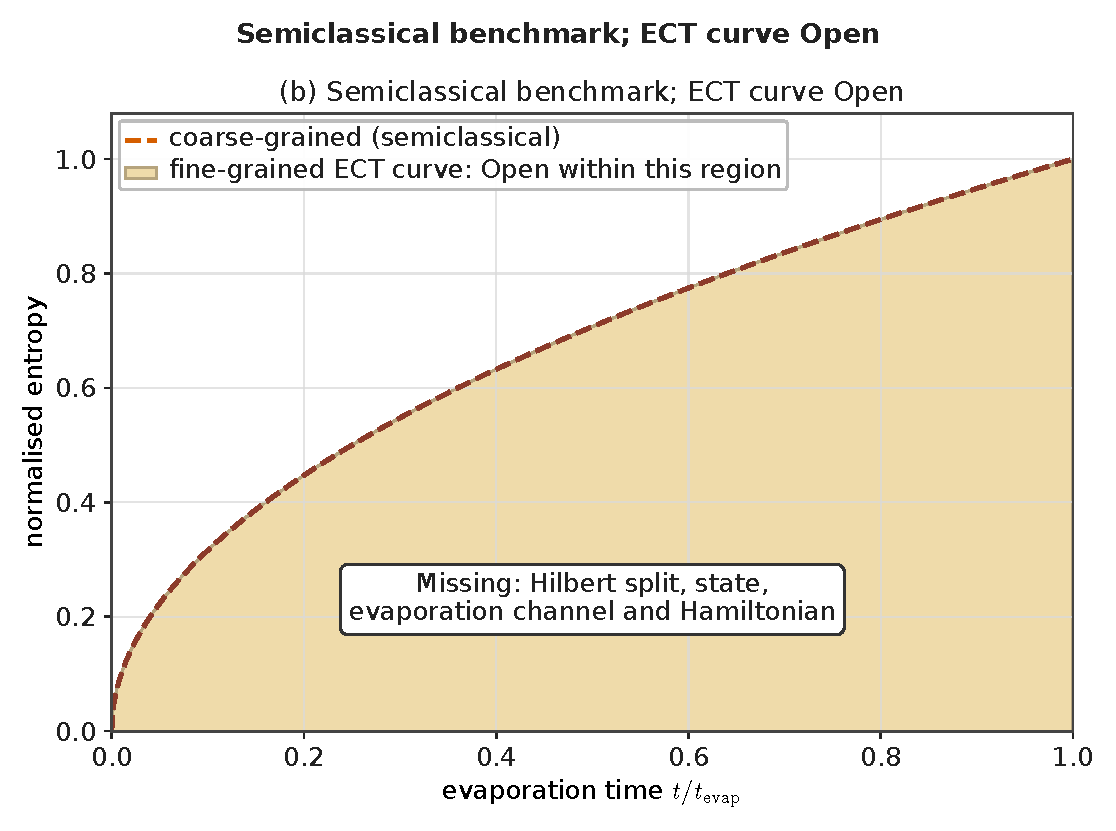
\includegraphics[width=\textwidth,height=0.58\textheight,keepaspectratio]{figures/r123/global/panels/fig35_b_page_curve_benchmark_r123.pdf}
\caption{Imported semiclassical coarse-grained entropy benchmark and
ECT status guard.  This page shows only the Page-curve benchmark.  The Open
region is not a predicted curve: the physical Hilbert-space split,
evaporation channel, state and Hamiltonian required for an ECT fine-grained
entropy history remain Open.  The Tolman near-horizon and Hawking-temperature
benchmarks are retained as separate full-width atlas panels; ECT presently
identifies no shell depth, critical surface or information-return law.}
\label{fig:bh_information}
\end{figure}

\FloatBarrier
Appendix~\ref{app:r129_visual_strong_field} preserves the separate Tolman and Hawking benchmark panels with the same Open-owner guard.
Figure~\ref{fig:bh_information} displays only external Tolman/Hawking
kinematics and the missing-owner inventory.  It is not a derived
near-horizon ECT structure.

\paragraph{Topological consistency of the shell picture.}
The supplied orientation target $O(4)/O(3)\simeq S^3$ has
$\pi_2(S^3) = 0$
(Section~\ref{sec:predicted_states}).
If a candidate shell is a closed two-surface $S^2$, the vanishing of
$\pi_2$ shows only that the restricted $n^A$ field carries no
$\pi_2$ charge.  It does not prove shell formation, stability,
dynamics, or coupling.  This is at most a consistency check:
if $\pi_2$ were nontrivial, the shell could trap topological charge,
potentially obstructing shell formation/dissolution and complicating
any evaporation scenario based on a finite-lifetime shell interface.
The nontrivial homotopy sector $\pi_3(S^3) = \mathbb{Z}$
(Section~\ref{sec:predicted_states}) admits topological configurations
of the exterior ordered-branch field;
however, the present work does not derive a stabilising
Skyrme-type higher-derivative term or a finite-energy gravitating
topological black-hole solution.

\paragraph{Connection to the UV-threshold and breakdown programmes.}
The strong-field toy is compared with the entanglement and
UV-threshold programmes, but equality of their states, kernels and
physical subsystem maps is not derived.
Whether a future action-owned P4 validity scale controls a physical
near-horizon breakdown is Open; the P3 curvature does not supply that
scale.
Using one branch-breakdown mechanism in cosmology and black holes is an
Open economy hypothesis, not a consequence of the common bare field.

\paragraph{Cross-sector consistency.}
The cosmological and black-hole singularity programmes explore a common
branch-breakdown hypothesis.  Neither replacement mechanism is yet
derived in the strong-field regime.
The completed theory may select a common mechanism or distinct
state-dependent mechanisms; neither outcome is imposed here.
Both illustrative programmes reuse the one-real-scalar toy temperature
$T_c = 2\phi_0$ and the same bare order parameter; this does not identify
the P4 gradient-ordering transition:
using the same $Z_2$ toy in both settings does not show that a
cosmological branch emerges thermally or that a black-hole branch
dissolves.  That proposed common mechanism is Open.

\paragraph{Discriminant with respect to alternative singularity
programmes.}
The ECT singularity programme differs from two common alternatives:
\begin{enumerate}[label=(\roman*)]
  \item \textbf{Classical-GR singularity realism:}
  the candidate programme tests whether the divergence marks branch
  failure; it does not establish that interpretation;
  \item \textbf{Bounce-by-postulate models:}
  ECT does not simply replace the singularity by a bounce imposed from
  outside; it asks whether loss of validity of the ordered geometric
  branch can be derived and leaves the microscopic completion as an
  open condensate-dynamics problem.
\end{enumerate}
This is an Open alternative to both fully specified bounce models and
unmodified extrapolation of classical GR to infinite curvature; its
relative viability cannot be ranked before a strong-field completion is
derived.

\paragraph{Falsifier for the singularity-breakdown programme.}
The present ECT singularity programme would be seriously weakened if a
completed condensate analysis showed that the ordered Lorentzian branch
remains fully valid all the way to the formal GR singularity with no
critical-shell, no pre-ordered transition, and no condensate breakdown
regime.
It would also be weakened if the only consistent completion of the
theory forced one back to a physically fundamental divergent
singularity rather than to a branch-boundary interpretation.
Conversely, an independently established critical regime before a classical
singularity would motivate this class of completion, but would not identify
the ECT action, state, or response mechanism.

\subsection{Observational anchors and the Open black-hole programme}
\label{sec:bh_obs_anchors}

\paragraph{External observations and constraints.}
The following observations constrain future strong-field completions but
currently provide neither compatibility evidence nor support for the ECT
black-hole programme.
The published Event Horizon Telescope comparison of the 2017 and
2018 M87* observations finds a persistent same-scale ring/shadow
structure~\cite{EHT2024M87}.  This owns the empirical persistence statement;
it does not identify an ECT horizon response, interior, or surface
mechanism.
Gravitational-wave ringdown tests remain broadly consistent with
Kerr-like exterior behaviour.  The present ECT candidate supplies no owned
strong-field action/state, exterior metric solution, interior/subsystem map,
radiation response or likelihood, and therefore makes no derived statement
about these data.  They are external targets for a future
exterior/interior completion, not consistency anchors for it.

\paragraph{Conditional geometric thinness of a supplied layer.}
For a non-extremal black hole and a supplied transition temperature
$T_*$, the Tolman toy defines
$\rho_*=\hbar c/(2\pi k_B T_*)$.
Relative to the Schwarzschild radius
$r_s=2G_N M/c^2$,
this gives
\begin{equation}
  \frac{\rho_*}{r_s}
  =
  \frac{\hbar c}{2\pi k_B T_* r_s},
  \label{eq:rho_c_over_rs}
\end{equation}
so thinness is conditional on the still-unidentified physical $T_*$.
No exterior-deviation bound follows from the present toy alone.
Timing observables, late-time correlations and horizon reflectivity
require a derived metric/transfer map.  No exhaustive experimental
channel can be selected before that map exists.

The present shell construction is developed for the non-rotating
(Schwarzschild) case.
For Kerr black holes the Tolman relation is modified by
rotation and the critical-shell radius may depend on latitude;
the analysis of this extension is left to future work.

\paragraph{Connection to the analogue-laboratory programme.}
The ordered-medium reading of horizon thermality finds its closest
controlled analogue in superfluid and BEC experiments where sonic
horizons generate phononic analogues of Hawking-like radiation
(\S\ref{sec:analogue_lab}).
These systems test their own ordered-medium horizon models.  An
analogue-to-ECT map is missing, so they currently provide motivation
rather than a test of the optional ECT shell completion.

\paragraph{Acceptance criteria for the optional shell completion.}
The shell ansatz becomes physical only if a completed action derives
its interface/control observable, subsystem algebra, state, radiation
vertex and observable metric, while reproducing the semiclassical
Hawking target where applicable.  A Page curve then requires the full
evaporation channel and state; the displayed tensor-product split does
not select it.

Failure of any of these gates rejects this shell completion only.
P1--P6 may admit a different strong-field completion, and no common
mechanism with cosmological branch breakdown is imposed in advance.

\paragraph{Summary in one sentence.}
The paradox is not solved: reduced-state thermality is compatible with
purity, while global ECT unitarity, the shell channel and information return
remain Open.

For a more explicit derivational sketch of the reduced-thermality logic,
the Hilbert-space factorisation, and the Page-curve discussion,
see Appendix~\ref{app:bh_reduced_thermality}.

\paragraph{Summary.}
Black-hole thermodynamics in ECT belongs to the Quantum Sector because
it probes the coherent-vacuum and reduced-state structure of the ordered
condensate.
The information paradox is decomposed into a generic reduced-state question
and an ECT-specific global-dynamics question.  Only the former is exact
mathematics under its stated Hilbert-space assumptions.  The globally
unitary completion, concrete shell implementation, subsystem map and
Page-curve-compatible evaporation route remain Open.
The full nonlinear strong-field completion remains open~(OP-Q13).

\subsection{Diagnostic discriminants across the gravity--matter interface}
\label{sec:qg_diagnostic_discriminants}

\textit{Status: compact cross-programme diagnostic summary. No new
physics is introduced; the table consolidates the status of three
focal frameworks along axes that discriminate them structurally and
observationally. Connection: the costs-of-consistency table of
Section~\ref{sec:costs_of_consistency} compared frameworks by
architectural cost; the present table instead compares them by
diagnostic signatures and structural commitments.}

Table~\ref{tab:qg_discriminants} summarises three focal frameworks
--- linearised-graviton effective field theory, the post-quantum
classical-gravity (PCCG) hybrid, and the ECT candidate
common-medium programme --- along six diagnostic axes relevant to the
gravity--matter interface.

\renewcommand{\arraystretch}{1.3}
\begin{longtable}{@{}L{3.5cm}L{3.8cm}L{3.7cm}L{3.7cm}@{}}
\caption{Cross-programme diagnostic discriminants among three
frameworks for the gravity--matter interface. Entries summarise
current structural and experimental commitments; detailed
references are in the surrounding text and in the cited
sections.}
\label{tab:qg_discriminants}\\
\toprule
Axis & Linearised-graviton EFT & PCCG / Oppenheim hybrid & ECT candidate programme \\
\midrule
\endfirsthead
\toprule
Axis & Linearised-graviton EFT & PCCG / Oppenheim hybrid & ECT candidate programme \\
\midrule
\endhead
\bottomrule
\endfoot
Independent metric quantisation
 & Yes (fundamental)
 & No (classical metric)
 & Open/not identified: the present scalar characteristic map is not a
   physical metric or tensor completion \\
Fundamental stochasticity
 & No
 & Yes (fundamental stochastic law)
 & Open: neither fundamental stochasticity nor an exclusively reduced-state
   origin has been established \\
Global unitarity
 & Yes
 & No (intrinsic information loss)
 & Open; not implied by P2 or by the present reduced-state constructions \\
GIE status in mesoscopic protocols
 & Expected in standard protocols via nonclassical mediator exchange
 & Framework-dependent; the standard stochastic reading is not built around unitary mediator-induced entanglement, while loophole constructions exist in neighbouring hybrid classes
 & No protocol-level ECT prediction: the physical mediator, state, channel
   and apparatus coupling remain Open~(\S\ref{sec:ect_gie}) \\
Evaporation / information stance
 & Outside the scope of linearised EFT; the answer depends on a separate
   strong-field/ultraviolet completion
 & Intrinsic information loss in the named stochastic model
 & A thermal marginal is compatible with a supplied global isometry;
   ECT factorisation, thermality and evaporation dynamics Open~(\S\ref{sec:bh_info_paradox}) \\
Relation to islands/QES language
 & Outside linearised-EFT scope; islands belong to separate holographic
   strong-field constructions
 & No generic entry follows from the framework label alone
 & Analogy only: the ECT factorisation, generalized entropy and extremization
   rule are all Open~(\S\ref{sec:bh_islands_comparative}) \\
\end{longtable}

\paragraph{Reading the table.}
The rows are not logically independent: a framework's stance on
metric quantisation strongly constrains its stance on
stochasticity and on global unitarity. No single row uniquely
falsifies any framework; the table summarises the joint pattern of
commitments or open completion requirements recorded here.  In particular,
an Open ECT entry is not a prediction of the present action.

\paragraph{Scope and non-claims.}
The table does not claim
(i) that the three frameworks exhaust the space of gravity--matter
architectures (Newton--Schr\"{o}dinger-class, measurement-feedback
hybrids, and others remain);
(ii) that any individual cell is beyond revision with further work
in the respective framework;
(iii) that current experiments have decided between the
frameworks.
It is a structural cross-programme summary, not a verdict.

% ==============================================================

\paragraph{Bridge to the analogue-laboratory programme.}
The black-hole programme, including its comparative mapping to the
islands/QES language~(\S\ref{sec:bh_islands_comparative}) and the
cross-programme diagnostic summary~(\S\ref{sec:qg_diagnostic_discriminants}),
concerns the same ordered medium as the vacuum-response, decoherence,
and entanglement sections, but in a different regime.
The next section turns from the astrophysical strong-field regime to
controlled laboratory analogues, where horizons, mode conversion, and
effective thermal response can be studied in experimentally accessible
ordered media.

% ============================================================

% ==============================================================
\section{Analogue Laboratory Programme: Named Source-Model Tests}
\label{sec:analogue_lab}
% ==============================================================

\textit{Status: Level~A only for mathematics and measurements inside each
named laboratory source model; Level~B for a fully specified conditional
map between such a model and a declared ECT sector; Open for an ECT-specific
discriminator.  Existing analogue results are neither evidence for ECT nor
an ECT falsifier.  Connection: compact-phase winding
(\S\ref{sec:qs_conservation}), supplied vacuum-response models
(\S\ref{par:vacuum_programme}), open-system kernels
(\S\ref{par:decoherence_programme}), the quantum--classical boundary
(\S\ref{sec:quantum_classical_boundary}), horizon interfaces
(\S\ref{sec:qs_bh}), and medium character~(P5).}

\paragraph{Purpose and inference boundary.}
\label{par:analogue_programme}
Laboratory media can realise mechanisms that also appear in ECT candidate
constructions: compact phases, winding sectors, mode conversion, response
kernels and environment-sensitive coherence.  An experiment first tests the
action, state, operators and observables of its own source model.  Similarity
of mechanism is a comparison, not evidence that the ECT vacuum has the same
owner.  Conversely, failure of an analogue implementation rejects that
implementation, not ECT as a whole.

\paragraph{Minimum bridge contract.}
An analogue result becomes an ECT test only after one prespecified bridge
supplies all of the following:
\begin{enumerate}[label=(\roman*)]
  \item the laboratory source action and the candidate ECT action sector;
  \item the preparation/state and boundary or driving protocol on both sides;
  \item an operator or vertex map, including normalisation and domain;
  \item an observable map, calibration and finite-time measurement rule;
  \item uncertainty, nuisance and detector-response models; and
  \item a quantitative discriminator against the ordinary laboratory source
        model and other non-ECT explanations.
\end{enumerate}
Without these six owners there is no likelihood ratio or falsification
statement about ECT.  Shared words such as ``medium'', ``horizon'' or
``correlator'' do not supply the bridge.

\paragraph{Four retained mechanism classes.}
The earlier analogue inventory survives after this correction, but with
source-model ownership made explicit.
\begin{enumerate}[label=(\roman*)]
  \item \textbf{Compact phase and winding.}  Superfluid helium, atomic BEC
  and Josephson systems can have quantised circulation or flux and
  defect-mediated phase slips.  The topological statement is exact when the
  named order parameter remains nonzero on the contour.  BR1 has the same
  conditional topology only after its own complex field, domain and defect
  boundary are supplied.
  \item \textbf{Boundary, drive and horizon response.}  Superconducting
  circuits exhibit dynamical-Casimir mode production~\cite{Wilson2011}, and
  acoustic BEC experiments realise source-model horizon/mode-mixing
  observables~\cite{Steinhauer2016}.  Each follows from its platform action,
  state and detector.  Neither supplies an ECT Casimir, Unruh or Hawking
  owner.
  \item \textbf{Controlled decoherence.}  Matter-wave and circuit platforms
  can vary bath occupation, spectrum, correlation time and coupling.  This
  tests the declared influence-functional kernel.  It does not identify an
  ECT record vertex, environment split or universal collapse boundary.
  \item \textbf{Background sensitivity.}  Density, stiffness, condensate
  fraction and proximity to a transition can be controlled within one
  platform.  Correlated changes of response and coherence test that platform's
  action.  They do not establish the Open ECT dark-sector or galactic
  source/force map.
\end{enumerate}

\paragraph{Conditional statements retained inside named source models.}
Several useful tests remain sharp.  If a compact order parameter is nonzero
on a contour, its winding cannot change smoothly; a change requires a defect
or a crossing of the zero-amplitude set.  If one specified action, state and
operator generate several response channels, the corresponding kernels must
obey that source model's common spectral and response identities.  If a
declared bath owns decoherence, controlled changes of its spectrum and
occupation must change the measured coherence according to the same kernel.
If a common background parameter enters several operators, their responses
must follow the jointly propagated covariance.  These are falsifiable
source-model statements.  They become ECT statements only after the bridge
contract above is derived and frozen.

\paragraph{What existing experiments establish.}
Quantised circulation, phase slips, dynamical-Casimir radiation, acoustic
mode mixing and tunable environmental decoherence establish that the
corresponding mechanisms occur in their respective systems.  They demonstrate
physical possibility and provide test-bed technology.  They neither confirm
one universal condensate mechanism nor distinguish ECT from conventional
descriptions of those platforms.

\paragraph{Falsification hierarchy.}
A discrepancy is classified in order: instrument/resolution, preparation or
state, boundary/drive model, operator/vertex, kernel/counterterm convention,
observable map, and finally the named source-model claim.  An ECT claim is
reached only if the frozen analogue--ECT bridge and its discriminator have
survived every preceding check.  This preserves the operational M3 hierarchy
of Appendix~\ref{app:AP6G-shared-interpretation}: success is reported for the
declared protocol and channel, while failure names the first failed guard.

For the source-model dictionary, see
Appendix~\ref{app:analogue_dictionary}.

\statussummary
\textit{Established externally:}
the listed laboratory mechanisms inside their named source models and
protocols.  \textit{Conditional Level~B route:} a future six-owner bridge
can turn one of them into an ECT-sector test.  \textit{Open:} a current
ECT-owned bridge, quantitative discriminator and corresponding likelihood.

\paragraph{Summary.}
The analogue programme is retained as an experimental design programme, not
as empirical support already accumulated for ECT.  Its positive contribution
is concrete: it identifies controllable source models, guard variables and
observables with which a future ECT operator-level completion could be tested.

\paragraph{Operational M3 protocols.}
The ordered-branch record programme now carries three operational
falsification protocols, specified in
Appendix~\ref{app:AP6G-M3-operational-protocols}: the
intrinsic/external threshold contrast (M3-1), the zero-mode detector
(M3-2), and the Airy-width/fingerprint protocol (M3-3).
Their observable inputs are fixed by the width-sector interface of
Appendix~\ref{app:AP6E-width-observable-interface} and the threshold
package of Appendix~\ref{app:AP6D-threshold-protection}, with platform
mapping through the analogue-observable dictionary of
Appendix~\ref{app:analogue_dictionary}.
A failed protocol is interpreted through the failure hierarchy stated
there; it is not automatically a falsification of the wider framework.

\paragraph{Bridge to the status map.}
The analogue-laboratory programme completes the structural development
of the Quantum Sector.
The next section collects the results of the preceding Part~III sections into a single
status map, identifies the remaining open problems, and states the
completion status of Part~III as a whole.

% ==============================================================
\section{Status Map, Open Problems, and Completion Status of Part~III}
\label{sec:qs_status_map}
% ==============================================================

This section collects the results of the preceding Part~III sections into a single
status map, identifies the irreducible structural core that ECT has
already established, separates it from the closure-level and open
fronts, and states the completion status of the Quantum Sector as a
whole.
Section~\ref{sec:qs_status} presents the detailed row-by-row status
table and the open-problem list.
Section~\ref{sec:qs_minimal_core} organises the minimal quantum core
into a strict structural tier, a structurally singled-out backbone,
and the nearest closure-level or open fronts.
Section~\ref{sec:qs_bridge_forward} states the overall completion
status and provides the bridge from Part~III to the summary,
comparison, and outlook sections that follow.

\subsection{Status table and open problems of the Quantum Sector}
\label{sec:qs_status}
% backward-compatibility alias:
\label{sec:derivation_map}
% backward-compatibility alias:
\label{sec:open_problems}
% ============================================================

\textit{Purpose: to summarise what the Quantum Sector of ECT already
establishes structurally, what is presently available only at closure
level, and what remains open.
This subsection plays for the Quantum Sector the same r\^ole that the
final status table plays for Macroscopic Physics.
The assignments below reflect the architectural strengthening of
the preceding Part~III sections, including medium character~(P5), the
global/reduced unitarity distinction, the unified vacuum-response
programme, the decoherence/arrow-of-time architecture, the
quantum--classical boundary, and the ordinary projector-Gleason representation
of an independently supplied normalised, noncontextual, countably additive
projector measure on a complex Hilbert space with $\dim\mathcal H\ge3$;
physical application input~(C3) and the Busch effect/POVM theorem under separately declared C2q hypotheses for a qubit remain separate, followed by the entanglement
programme, the wider topological/dark-sector ontology, the conditional
black-hole information-preservation programme, and the analogue-laboratory
instantiability programme.}

\medskip
\paragraph{Methodological note on status levels.}
The strengthened postulate and branch structure improves the Quantum
Sector in an important but limited way.
In several places it still does not promote familiar quantum laws to
unconditional Level~A theorems.
Its real gain is subtler and more architectural:
it turns earlier heuristic claims into conditional structural
statements, removes overclaims, narrows the admissible logical
possibilities, sharpens the distinction between global and reduced
descriptions, while leaving the global information question explicitly Open.
The table below reflects these deliberately honest levels.

\medskip
The status map condenses the nineteen Part~III sections into the following
twelve reader-facing thematic steps (including the scope/inputs layer as the
first step).  Dedicated bridge modules are retained in their owning rows and
dependency links rather than counted as additional themes:
\begin{enumerate}[noitemsep,label=(\roman*)]
  \item scope, inputs, and logical programme of the Quantum Sector;
  \item coherent phase dynamics, loop sectors, and the pre-quantum
    action scale $S_0$;
  \item wave kinematics, common-length hyperbolic parametrisation,
    extremal-action structure,
    and conservation laws;
  \item Hilbert-space bridge: the complete applicable corrected OS-II package,
    including reflection positivity, followed by unitarity, canonical
    structure, and the uncertainty principle;
  \item Euclidean path-dependence, exchange sectors, and Dirac
    structure;
  \item quantum vacuum structure and the unified response programme
    (Casimir, Unruh, particle production, horizon thermality);
  \item open quantum systems, decoherence, and the arrow of time;
  \item quantum--classical boundary, probability, Born-type
    interpretation, and measurement status;
  \item quantum entanglement and Bell-type correlations;
  \item topological / defect sectors and the dark sector;
  \item black-hole thermodynamics, Hawking-type radiation, and the
    information problem;
  \item analogue laboratory programme.
\end{enumerate}
The resulting picture is already substantial, but deliberately not
overclaimed.
Figure~\ref{fig:qs_consistency} and
Table~\ref{tab:qs_status} distinguish sharply between what is
structurally established, what is plausible within the current
coherent-sector closure, and what remains open.
The status table below should be read together with the open-problem
list and the dependency map: the table records local status row by row,
the map records logical dependence, and the open-problem list records
what is still needed for programme closure.

{
\small
\renewcommand{\arraystretch}{1.35}
\begin{longtable}{@{}L{6.7cm}L{2.7cm}L{5.1cm}@{}}
\caption{Status map of the Quantum Sector of ECT.
Level~A = exact in the declared model and assumptions, with an explicit reproducible derivation; reproducible checks verify
that derivation but do not replace it; it does not by itself establish descent from P1--P6 or
physical ECT ownership.
Level~A/B = an explicit Level~A algebraic or obstruction result paired
with a Level~B structural/conditional route whose physical
identification or full closure remains open.
Level~B = structural/conditional derivation or closure route with a
declared open matching, input, or identification step.
Open = not yet derived; where available, an explicit open-problem
reference is given.}
\label{tab:qs_status}\\
\hline\hline
Statement / claim & Status & Basis / comment \\
\hline
\endfirsthead
\hline\hline
Statement / claim (cont.) & Status & Basis / comment \\
\hline
\endhead
\hline
\endfoot
\hline\hline
\endlastfoot
Statement / claim & Status & Basis / comment \\
\hline
% --- Ch.19--20: Scope, phase dynamics, S_0 ---
Supplied coherent $U(1)$ phase-sensitive sector
  & Level~B / supplied closure
  & Not implied by the real P3 scalar; Section~\ref{sec:qs_intro} \\
Phase variable $\theta$ inside that supplied compact sector
  & Level~B / supplied closure
  & Section~\ref{sec:qs_phase_dynamics} \\
Integer winding sectors exist
  & Level~A mathematics conditional on the supplied compact phase
  & Single-valuedness of $\Phi_{\rm eff}$;
    Eq.~\eqref{eq:qs_winding} \\
Phase-only fixed-core reduced-coefficient candidate
$\iota_{\rm elem}^{(\rm fixed\ core)}=2\pi \iota_0^{\rm EFT}$
  & A fixed-$L$ mathematics / B-Open closure
  & Defined by evaluating the fixed-length phase-gradient functional at a
    supplied core scale; not a global minimum and not fixed by topology \\
Tension-balanced finite-loop minimum
$\mathcal I_{1,\min}=2\pi \iota_{0,\rm bal}^{\rm eff}$
  & A mathematics / B-Open ECT route
  & Exact for the supplied positive-tension 1D functional; the tension,
    common 4D reduction and unwinding/backreaction completion are Open \\
First-principles physical action scale
  & Open (OP-Q1)
  & Derive or refute $K_\theta^{1\mathrm D}$ and
    $\mathcal T_{\rm loop}$ from one 4D owner, then test universality;
    Appendix~\ref{app:Sloop_calc} \\
Operational $S_0$ and the identification $S_0=\hbar$
  & Level~B calibration / Open owner
  & Either loop candidate requires its own owner map to the operational
    slot; the calibration is explicit, while its absolute derivation and
    cross-sector universality are independent Open tests;
    Eq.~\eqref{eq:qs_S0_identification} \\
% --- Ch.21: Wave kinematics, extremal action, conservation ---
Hamilton--Jacobi / continuity decomposition
  & A mathematics given a supplied complex evolution law; ECT owner B/Open
  & Polar split alone supplies no Hamiltonian, current, domain, or dynamics;
    Section~\ref{sec:qs_wave} \\
Probability-current reading of a supplied complex continuity law
  & B/Open
  & Requires the complex law, state, inner product, domain, clock and physical
    matching; it is not the compact-phase Noether current \\
Schr\"odinger-type complex recombination
  & Level~B
  & Structural route; $S_0=\hbar$ and $\hat H_{\rm coh}$ still needed;
    Eq.~\eqref{eq:qs_schrodinger_type} \\
Lorentzian stationary-phase asymptotic
  & A-math conditional / B/Open ECT owner
  & Requires a supplied oscillatory integral; the Euclidean extremum has
    distinct dominance conditions \\
Declared conservation laws in their owning actions
  & A within each supplied action
  & Real-scalar Noether currents and compact-phase EFT current are distinct;
    no common probability-current owner follows \\
% --- Ch.22: Hilbert-space bridge ---
Reflection positivity in massive Gaussian broken-phase subsectors
  & Level~A mathematics in supplied free model
  & Section~\ref{sec:qs_reflection_positivity};
    RP plus the standard free-scalar covariance, symmetry, regularity,
    locality and clustering package \\
Reflection positivity in free massless Goldstone-coordinate Gaussian subsectors
  & Level~A mathematics in supplied free model
  & Section~\ref{sec:qs_reflection_positivity};
    standard local massless-scalar OS package after the infrared/zero-mode
    domain is fixed; physical mode count remains Open \\
Reflection positivity for full interacting coherent sector
  & Open (OP-Q16)
  & Section~\ref{sec:qs_reflection_positivity};
    constructive QFT programme \\
Global unitarity in reconstructed positive Gaussian subsectors
  & Level~A mathematics in supplied free models
  & Follows only after the complete applicable corrected Gaussian OS-II
    hypothesis set,
    not from reflection positivity alone;
    Section~\ref{sec:qs_unitarity_status} \\
Global unitarity beyond Gaussian regime
  & Level~B/open
  & Depends on OP-Q16; not yet independently established;
    Section~\ref{sec:qs_unitarity_status} \\
Global vs.\ reduced unitarity distinction
  & Level~A
  & Well-defined structural distinction between full coherent unitarity
    and reduced-sector effective non-unitarity;
    Section~\ref{sec:qs_unitarity_status} \\
Canonical organisation of smooth coherent branch
  & Level~A mathematics in supplied reduced model
  & Section~\ref{sec:qs_ccr};
    $\pi_\theta^{\rm phys}=\Sigma_\theta\pi_\theta^{\rm red}$ for a finite
    positive constant $\Sigma_\theta$ \\
Poisson brackets of coherent canonical variables
  & Level~A mathematics in supplied reduced/physical symplectic normalisations
  & Eq.~\eqref{eq:qs_poisson}; the reduced and physical brackets must not be
    mixed \\
Local-chart physical-momentum commutator candidate normalised by $S_0$
  & Level~B/Open
  & Eq.~\eqref{eq:qs_commutator_candidate};
    $[\theta,\pi_\theta^{\rm phys}]=iS_0\delta$, equivalently
    $[\theta,\pi_\theta^{\rm red}]=i(S_0/\Sigma_\theta)\delta$ on a declared
    common core; no global self-adjoint angle CCR is claimed \\
Integer winding of the compact phase field
  & Level~A topology in supplied smooth compact-field domain
  & Eq.~\eqref{eq:qs_winding}; independent of a canonical-generator spectrum \\
Canonical compact-shift-orbit generator spectrum
  & Level~A operator mathematics under supplied Weyl representation and
    self-adjoint domain / B/Open physical ECT owner
  & Eqs.~\eqref{eq:qs_Qtheta}--\eqref{eq:qs_dirac_quantization};
    $[\hat Q_\theta^{\rm phys},U_0]=S_0U_0$ and spectrum
    $S_0(\mathbb Z+\nu_{\rm tw}/2\pi)$, reducing to $S_0\mathbb Z$ only for
    the supplied periodic domain $\nu_{\rm tw}=0$ \\
Momentum-operator-type wave kinematics
  & Level~B
  & Eq.~\eqref{eq:qs_p_operator}; depends on the physical $S_0$
    normalisation and representation \\
Full operator algebra and many-body canonical completion
  & Open (OP-Q4)
  & Section~\ref{sec:qs_ccr};
    operator-level derivation beyond the reduced coherent sector \\
Uncertainty inequality $\Delta q\,\Delta p_{\rm phys}\ge S_0/2$
  & Level~A operator mathematics conditional / B--Open physical owner
  & Eqs.~\eqref{eq:qs_robertson}, \eqref{eq:qs_uncertainty_S0};
    applies to a supplied self-adjoint noncompact canonical pair with common
    product domains, not automatically to the compact angle and rotor \\
Heisenberg form $\Delta q\,\Delta p_{\rm phys}\ge\hbar/2$
  & Level~B calibration / Open owner
  & Requires the separate match $S_0=\hbar$~\eqref{eq:qs_S0_identification} \\
% --- Ch.23: Path-dependence, statistics, Dirac ---
Two-sided Euclidean boundary dependence
  & Level~A
  & Elliptic Euclidean field equation;
    Section~\ref{sec:path_dependence} \\
Interference/tunnelling route from Euclidean methods
  & Level~B route / Open physical ECT
  & Two-sided elliptic dependence is Level-A BVP mathematics but is neither
    sufficient nor discriminating.  Interference additionally needs an
    admitted quantum measure/coherent structure, composable kernel,
    state/preparation and observable map; tunnelling needs a named
    action/saddle, state, boundary/continuation prescription,
    determinant/prefactor and detector map.  No ECT-specific amplitude or rate
    is derived; Sections~\ref{sec:path_dependence}
    and~\ref{sec:pes_tunnelling} \\
Indefinite-causal-order compatibility route
  & Level~B
  & Structural reading only; quantitative switch reconstruction open;
    Section~\ref{sec:indefinite_causal_order} \\
Visibility proxy for the quantum-switch source model
  & Source-model / ECT Open
  & $\Phi_{\rm vis}=-\ln V$ is an observational transform, not a universal
    degradation law; Eq.~\eqref{eq:indef_causal_criterion} \\
Topological exchange-sector dichotomy ($\mathbb{Z}_2$)
  & Level~A conditional topology / physical ECT map Open
  & $\pi_1(\mathcal M_2)=\mathbb Z_2$ for two supplied identical unlabeled
    points in defect-free $\mathbb R^3$; the physical spatial/excitation map
    and representation selection remain Open;
    Section~\ref{sec:qs_statistics} \\
Spatial dimensionality $d_{\rm spatial}=3$ fixes the exchange topology
  & Level~A conditional / physical slice Open
  & Given a separately supplied three-dimensional spatial slice,
    $\pi_1(\mathcal{M}_2)=\mathbb{Z}_2$; P4 alone does not derive that slice;
    Section~\ref{sec:qs_statistics} \\
Bosonic/fermionic structural compatibility
  & Level~B
  & Exchange topology plus ordered-branch representation content;
    Section~\ref{sec:qs_statistics} \\
Abstract $\mathfrak{so}(4)\to\mathfrak{so}(1,3)$ generator continuation
  & Level~A conditional mathematics
  & Standard complex continuation after its map is supplied; not a physical
    metric derivation; Section~\ref{sec:qs_dirac} \\
Clifford representation
  $\{\gamma_L^\mu,\gamma_L^\nu\}=-2g^{\mu\nu}$
  & Level~A conditional mathematics / Open ECT owner
  & Requires supplied metric, tetrad and spinor representation \\
Dirac-type free dynamics for realised spinorial excitations
  & Level~B~(conditional)
  & Only inside the supplied four-complex-component irreducible
    Clifford-factorisation class: physical Lorentzian metric/tetrad and spin
    structure, $(\tfrac12,0)\oplus(0,\tfrac12)$ module, local linear
    constant-coefficient Lorentz covariance and exact KG factorisation;
    reducible, constrained/gauge and non-Clifford systems lie outside;
    Eq.~\eqref{eq:qs_dirac_conditional};
    Section~\ref{sec:qs_dirac} \\
Physical spinorial sector of ECT
  & Open~(OP-Q11)
  & Requires metric/spinor descent, spectrum, CAR/Fock construction and state \\
Pauli exclusion
  & Level~B~(conditional)
  & From Dirac structure + spin-statistics argument;
    conditional on $S_0=\hbar$~(OP-Q2) \\
Full spin-statistics theorem
  & Open (OP-Q11)
  & Requires operator completion beyond current closure; the
    free-kernel Euclidean OS test is now Level~A (Q11.1a,
    Section~\ref{sec:fermion_statistics}) \\
Spin discreteness / Stern--Gerlach selection
  & A-math conditional / B / Open
  & Discreteness is standard compact-$SU(2)$ representation mathematics
    after a physical rotation/spinor sector is supplied; its ECT owner,
    apparatus channel, outcome and update remain Open;
    Section~\ref{sec:qs_dirac} \\
% --- Ch.24: Vacuum response ---
Supplied ordered/coherent models have nontrivial correlator and stiffness
structure
  & Level~A inside the supplied reduced models / physical ECT vacuum Open
  & A physical common ECT vacuum still requires its state, operator/bundle,
    continuation, couplings and response ownership;
    Section~\ref{sec:qs_vacuum_intro} \\
Supplied soft-sector boundary-value response
  & Level~A mathematics / B--Open physics
  & Each declared operator and boundary condition has a calculable mode
    response; the physical condensate boundary and ordinary-matter coupling
    are not derived; Section~\ref{sec:qs_casimir} \\
Supplied scalar Dirichlet coefficient
  & Level~A mathematics / Open ECT
  & Eq.~\eqref{eq:casimir_ect}; physical mode count, material boundary
    map and stress response are missing \\
Euclidean--Rindler/KMS route
  & Level~A external / Open ECT
  & The standard response follows only after supplying the physical metric,
    state/KMS condition, detector coupling and clock/action matchings;
    Section~\ref{sec:qs_unruh} \\
Unruh temperature formula in the supplied route
  & Level~A external / Open ECT
  & Eq.~\eqref{eq:unruh_ect}; requires $S_0=\hbar$, a physical cone,
    and the missing detector/state owners;
    Section~\ref{sec:qs_unruh} \\
Time-dependent ordered backgrounds: background-dependent particle notion
  & Level~A external / Open ECT
  & Standard after a time-dependent action and in/out states are supplied;
    ECT ownership Open; Section~\ref{sec:qs_particle_production} \\
Bogoliubov-type mode mixing in ECT coherent vacuum
  & Level~A external / Open ECT
  & Eq.~\eqref{eq:qs_bogoliubov}; ECT action, states, particle map and
    quantitative rates open (OP-Q12);
    Section~\ref{sec:qs_particle_production} \\
Quantitative production rates $|\beta_k|^2$
  & Open (OP-Q12)
  & Requires completed time-dependent coherent-vacuum calculation \\
Horizon-thermality comparison
  & Level~A external / Open ECT
  & Standard Hawking target; requires an independently completed physical metric, quantum state and
    strong-field sector; Sections~\ref{sec:qs_vacuum_unified},
    \ref{sec:qs_bh} \\
Common vacuum-response programme (Casimir/production/Unruh/horizon)
  & Open
  & Section~\ref{sec:qs_vacuum_unified}; a proposed common architecture,
    not one response operator derived for all four regimes \\
Analogue-gravity source-model comparison for coherent-vacuum mechanisms
  & External source-model results / ECT Open
  & Section~\ref{sec:qs_vacuum_unified}; mechanism comparison is not
    evidence for ECT and no analogue result is a generic ECT falsifier \\
% --- Ch.25: Decoherence, arrow of time ---
Reduced influence-functional organisation
  & Level~B
  & Open-system EFT of coherent branch;
    Eq.~\eqref{eq:qs_influence} \\
Retarded propagation of ordered-branch scalar~$\Phi$
  & Level~A (quadratic)
  & Appendix~\ref{app:retarded_kernel} \\
Nonnegative spectral measure $\rho(\mu^2)\ge0$
  & Level~A conditional / ECT owner Open
  & Follows only for a supplied positive Hilbert/state/observable and residue
    representation or explicit positive oscillator decomposition; it is not
    derived by the classical broken-phase Hamiltonian alone \\
Three-dimensional derivative-coupling bath toy gives
$J_{\rm bare}\!\propto\!\omega^4$ and $J_W\!\propto\!\omega^3$
  & Level~A conditional mathematics within a supplied quadratic bath
  & Not a derived ECT record channel; vertex- and state-dependent;
    Eq.~\eqref{eq:qs_super_ohmic} \\
Effective ohmic regime
  & Model ansatz
  & Not derived from the minimal bath; Eq.~\eqref{eq:qs_ohmic} \\
Markov approximation
  & Model condition
  & Insufficient for monotone entropy; Eq.~\eqref{eq:qs_markov} \\
Low-entropy initial-branch interpretation
  & Open
  & Requires a measure, coarse graining, and state-selection rule;
    Section~\ref{sec:qs_decoherence} \\
Entropy monotonicity theorem for an ECT reduced channel
  & Open
  & Requires the normalised channel/state, entropy functional, and
    unitality/detailed-balance/contractivity hypotheses; OP-Q17 \\
Protocol-defined Crooks fluctuation relation
  & Open
  & Requires forward/reverse path measures, time reversal, initial ensembles,
    and local detailed balance; Eq.~\eqref{eq:crooks_ECT} is a definition only \\

C$_{60}$ collisional-decoherence source-model anchor
  & External observation / source model / ECT Open
  & Interference is retained from Arndt et al.~\cite{Arndt1999}; the exact
    pressure sub-number lacks an identified primary owner and is not quoted;
    no distinct ECT rate is published;
    Section~\ref{sec:tau_ECT_systems} \\

Di\'osi--Penrose external comparison
  & External formula and Level-C hard-sphere point / ECT Open
  & $C_{\rm DP}(1)=51/160$ and $70.6\,\mathrm{ms}$ only for the declared
    continuum geometry; ECT projector, vertex, state, noise and absolute
    normalisation not identified; Section~\ref{sec:pes_diosi} \\
Common influence-functional notation
  & Level~B organisational / physical identification Open
  & Does not establish one bath or one kernel for environmental and
    gravitational channels \\
% --- Ch.26: QC boundary, Born, measurement ---
Physical reverse $O(3)\!\to\!O(4)$ segment mechanism
  & Open
  & Ordinary Euclidean boundary dependence does not establish physical
    reverse segments, their weight, or a laboratory threshold;
    Section~\ref{sec:path_dependence} \\

Reduced-state dephasing / record crossover
  & Level~B/Open
  & Channel- and protocol-specific; does not change metric signature or select
    a unique outcome; Section~\ref{sec:quantum_classical_boundary} \\

Pure-dilation qubit mutual-information toy
  & Level~A model algebra / ECT Open
  & Total system--environment mutual information in the declared toy, not
    accessible detector information or a protocol-independent bound;
    Section~\ref{sec:pes_info_bound} \\

Wigner's-friend reduced-state record reading
  & Interpretive / Open
  & A specified coarse graining can form records; pointer basis, unique
    outcome, and update remain Open;
    Section~\ref{sec:quantum_classical_boundary} \\

Echo/control recoherence
  & Standard channel result / ECT Open
  & No Lorentzian-to-Euclidean signature reopening or physical
    $O(3)\!\to\!O(4)$ backreaction map is derived;
    Section~\ref{sec:path_dependence} \\

Amplitude / decoherence / probability distinction
  & Level~A logic under supplied state/channel
  & Decoherence can suppress coherences but does not create a measure or
    outcome; Section~\ref{sec:qs_born}; Eq.~\eqref{eq:qs_prob_logic} \\
Admitted projector measure: conditional ordinary Gleason representation
  & Level~A mathematics under theorem hypotheses / ECT Open
  & Unique trace representation only for an independently supplied normalised,
    noncontextual, countably additive projector measure on a complex Hilbert
    space with $\dim\mathcal H\ge3$; a qubit requires the Busch effect/POVM theorem under separately declared C2q hypotheses.  State/preparation, event, probability
    origin, outcome and update remain Open~(OP-Q7) \\
Independent inputs (C1), (C2) or (C2q), and (C3) for the conditional Gleason representation
  & Conditional / Open ECT ownership
  & (C1) supplied Hilbert/event algebra; (C2) supplied projector measure
    in complex dimension at least three, or separately declared C2q
    full-effect measure hypotheses in dimension two; (C3) supplied
    preparation plus projector/effect event map.  A
    dephasing channel is a separate application layer;
    Section~\ref{sec:qs_born} \\
Unique outcome selection beyond an admitted physical probability-weight map
  & Open (OP-Q19)
  & Relation between branch weights, decohered alternatives, and
    actually realised records remains incomplete;
    Section~\ref{sec:qs_born} \\
Full Born rule as first-principles theorem
  & Open (OP-Q7)
  & Requires physical derivation of the state/preparation, event map,
    probability origin, outcome and update from coherent-sector dynamics \\
Completed measurement-update theory
  & Open (OP-Q8)
  & Pointer sectors, branch update, records not complete \\
% --- Ch.27: Entanglement ---
Non-factorisable coherent correlations (entanglement route)
  & Standard conditional mathematics / ECT Open
  & Requires a supplied nonfactorising state/channel; a single medium does not
    force nonfactorisation;
    Section~\ref{sec:qs_entanglement} \\
No-signalling compatibility of common-medium entanglement
  & Conditional / ECT Open
  & Must be verified for the supplied state and local measurement channel;
    Section~\ref{sec:qs_entanglement} \\
Bell-correlator completion
  & Open (OP-Q20)
  & Must derive the physical preparation, state-or-configuration owner,
    settings, measurements and full joint outcome law, together with
    no-signalling and the Tsirelson restriction.  If a hidden/configuration
    representation is claimed, it must additionally supply a positive
    measure, response maps and causal/intervention semantics and determine
    rather than assume measurement independence and Bell factorisability;
    Section~\ref{sec:qs_entanglement} \\
Werner-state CHSH visibility marker
  & Source-model toy / ECT Open
  & $\Phi_{\rm vis}^{\rm Bell}=\ln\sqrt2$ follows from the declared Werner
    proxy; it is not an ECT Bell-correlator derivation;
    Section~\ref{sec:qs_entanglement} \\
Entanglement--tunnelling relationship
  & Interpretive / ECT derivation Open
  & The phenomena retain separate dynamical owners; no common suppression
    scalar or derivation of one from the other is claimed;
    Section~\ref{sec:qs_entanglement} \\
% --- Ch.28: Topological / defect / dark ---
Wider defect sector beyond smooth coherent branch
  & Level~A
  & Section~\ref{sec:qs_defects} + \ref{sec:defect_sectors} \\
Defect sectors: structural existence
  & Level~A
  & Section~\ref{sec:qs_defects} \\
Defect sectors: full dynamics and classification
  & Open (OP-Q9)
  & Core structure, stability, production; not yet complete \\
Smooth collective dark-sector candidates
  & Level~B
  & Bridge MP to QS; Section~\ref{sec:dark_sector} \\
Topological/defect dark-sector candidates
  & Level~B
  & Section~\ref{sec:qs_defects}; detailed dynamics open \\
Quantitative dominant dark-matter identification
  & Open (OP-Q10)
  & No unique first-principles candidate established yet \\
% --- Ch.29: Black holes ---
Black-hole thermodynamics as an external effective target
  & A external / Open ECT
  & Eqs.~\eqref{eq:qs_Hawking_temp}--\eqref{eq:qs_Hawking_temp_S0};
    rewriting requires $S_0=\hbar$ \\
Reduced-state thermality $\neq$ fundamental information loss
  & Level~A
  & General QS reduced-state logic;
    Eq.~\eqref{eq:qs_rho_ext} \\
Global information preservation in an interacting ECT completion
  & Open / conditional
  & Reduced-state thermality is compatible with purity (A mathematics),
    but P2 does not construct a Hilbert space or prove global interacting
    unitarity; Section~\ref{sec:qs_black_holes} \\
Candidate ordered-phase shell near the horizon
  & Level~C/Open
  & Section~\ref{sec:qs_black_holes}; supplied strong-field ansatz \\
Generalized entropy $S_{\rm gen}=S_{BH}+S_{\rm ext}^{\rm coarse}$
  & A external bookkeeping / Open ECT
  & Eq.~\eqref{eq:qs_generalized_entropy};
    natural reduced-observer bookkeeping \\
Page-curve-compatible unitary evaporation logic
  & A mathematics under supplied isometry / Open ECT
  & Does not select a Page curve; Section~\ref{sec:qs_black_holes} \\
Explicit Page-curve computation
  & Open (OP-Q13)
  & Requires global nonlinear shell dynamics \\
Full strong-field evaporation completion~(Page curve)
  & Open (OP-Q13)
  & Global nonlinear horizon solution not yet complete \\
Strong-field observable response
  & Open
  & No ECT dispersion, energy-response, ringdown, echo or
    primordial-black-hole correction is derived \\
% --- Ch.30: Analogue lab ---
Named analogue source-model mechanisms
  & External Level~A only inside each supplied platform model
  & Compact phase, winding, response and decoherence mechanisms are
    experimentally accessible; not evidence for ECT and not an ECT falsifier \\
Analogue--ECT operator-level bridge
  & Open
  & Requires action, state, operator, observable, uncertainty and
    discriminator maps; Section~\ref{sec:analogue_lab} \\
% --- Ch.26: Decoherence results and regime estimates ---
Visibility-derived dephasing proxies
  & Source-model / ECT Open
  & Procopio and Jacques values are $\Phi_{\rm vis}=-\ln V$ transforms;
    no ECT record kernel is inferred; Section~\ref{sec:decoherence_results} \\
Werner-state CHSH marker $\Phi_{\rm vis}=\ln\sqrt2$
  & Source-model toy / ECT Open
  & Eq.~\eqref{eq:Gamma_Bell_crossover}; no universal boundary or ECT
    discriminator; Section~\ref{sec:decoherence_results} \\
% --- Ch.27: PES ---
PES-R response--persistence taxonomy
  & Level~B / ECT inputs Open
  & Dynamical admissibility, finite-time retention, and pairwise records are
    distinct; no universal intersection or quantisation/Born/outcome theorem;
    Section~\ref{sec:pes} \\

% --- P6 spectral-record appendices (frozen) ---
Frozen P6 spectral-record framework (record kernels, dephasing
classes, line/ribbon records, threshold protection, width interface,
P26 over-closure)
  & Level~B
  & Frozen with non-proliferation guard;
    Appendices~\ref{app:AP6A-conventions-kernels}--\ref{app:AP6H-honesty-correction-index} \\
M3 operational falsification protocols (M3-1/2/3)
  & Level~B
  & Appendix~\ref{app:AP6G-M3-operational-protocols}; reporting packet
    and failure hierarchy specified \\
Analogue-platform execution of the M3 protocols
  & Open
  & Platform selection open (frozen-ledger item O4);
    Appendix~\ref{app:AP6G-M3-operational-protocols} \\
% --- QG/decoherence upgrade layer (Sections 31--36) ---
Problem of time in ECT: owner hierarchy
  & Level~B/Open
  & P1 supplies no external time; P4 supplies a direction; scalar
    hyperbolicity, physical clock/lapse, record dynamics and thermodynamic
    arrow retain separate owners;
    Section~\ref{sec:phys_picture_ssb} \\
Conditional discriminants for named quantum-gravity/decoherence completions
  & Open premises / conditional tests
  & Exclusions apply only after a completion owns and preregisters the
    mediator, state, channel and global-dynamics commitments;
    Section~\ref{sec:qs_falsifiers} \\
Reduced-state resolution of the hybrid-consistency problem
  & Level~B (architectural)
  & Candidate reduced-state architecture, not a finished theory;
    Section~\ref{sec:ect_hybrid_consistency},
    Table~\ref{tab:hybrid_costs} \\
Two-level ontology (Level~I / IIa / IIb)
  & Level~B/Open architecture
  & Conditional bookkeeping; the interacting observable algebra, state,
    universal partition and concrete reduction maps remain Open;
    Section~\ref{sec:two_level_ontology} \\
Gravity-induced-entanglement channel
  & Open / \texttt{NOT IDENTIFIABLE}
  & External BMV classes are known; ECT mediator/vertex/state are absent;
    Section~\ref{sec:ect_gie} \\
Operational criterion for BMV no-go vs loophole regimes
  & External conditional result
  & Applicable only after a physical reduced mediator is derived;
    Section~\ref{sec:gie_operational_criterion} \\
Mediator taxonomy: scalar trace, fixed director, composite and tensor candidates
  & Terminal bounded ledger
  & Scalar vertex parametric; director missing vertex; full ECT channel not identifiable;
    Section~\ref{sec:ect_mediator_taxonomy} \\
Physical gravitational entangling mediator
  & Open
  & Requires nonzero two-body vertex, positive state and a proved nonfactorising reduced channel;
    Section~\ref{sec:delta_n_channel} \\
BMS, memory and soft-graviton sector
  & External completion tests
  & No ECT tensor charges, memory map or soft-graviton owner is identified;
    Section~\ref{sec:ect_ir_soft} \\
Islands/QES structural mapping onto critical-shell picture
  & Level~B/C
  & Structural alignment, not a derivation of $S_{\rm gen}$ or of
    replica wormholes from ECT;
    Section~\ref{sec:bh_islands_comparative},
    Table~\ref{tab:bh_islands_mapping} \\
Cross-programme diagnostic discriminants
  & Summary-level
  & Six axes comparing ECT common-medium with linearised-graviton
    EFT and PCCG-hybrid;
    Section~\ref{sec:qg_diagnostic_discriminants},
    Table~\ref{tab:qg_discriminants} \\

\end{longtable}
}

\paragraph{Selected status and dependency map.}
Figure~\ref{fig:qs_consistency} is a selected connected Part~III dependency
graph.  It keeps coherent-phase dynamics, the two distinct action-scale
candidates, the candidate T1 owner calculation, OS-II reconstruction,
canonical organisation, response/decoherence, PES-R, admitted measures,
Born-rule status, particle/statistics routes and quantum-gravity targets in
one connected view.  In particular, it contains no direct decoherence,
quantum--classical-boundary or unitarity derivation edge into the Born node.
The OS-II/Hilbert route supplies event structure only under its full stated
hypotheses; an independently admitted measure and the physical
state/preparation, probability, outcome and update owners remain Open.

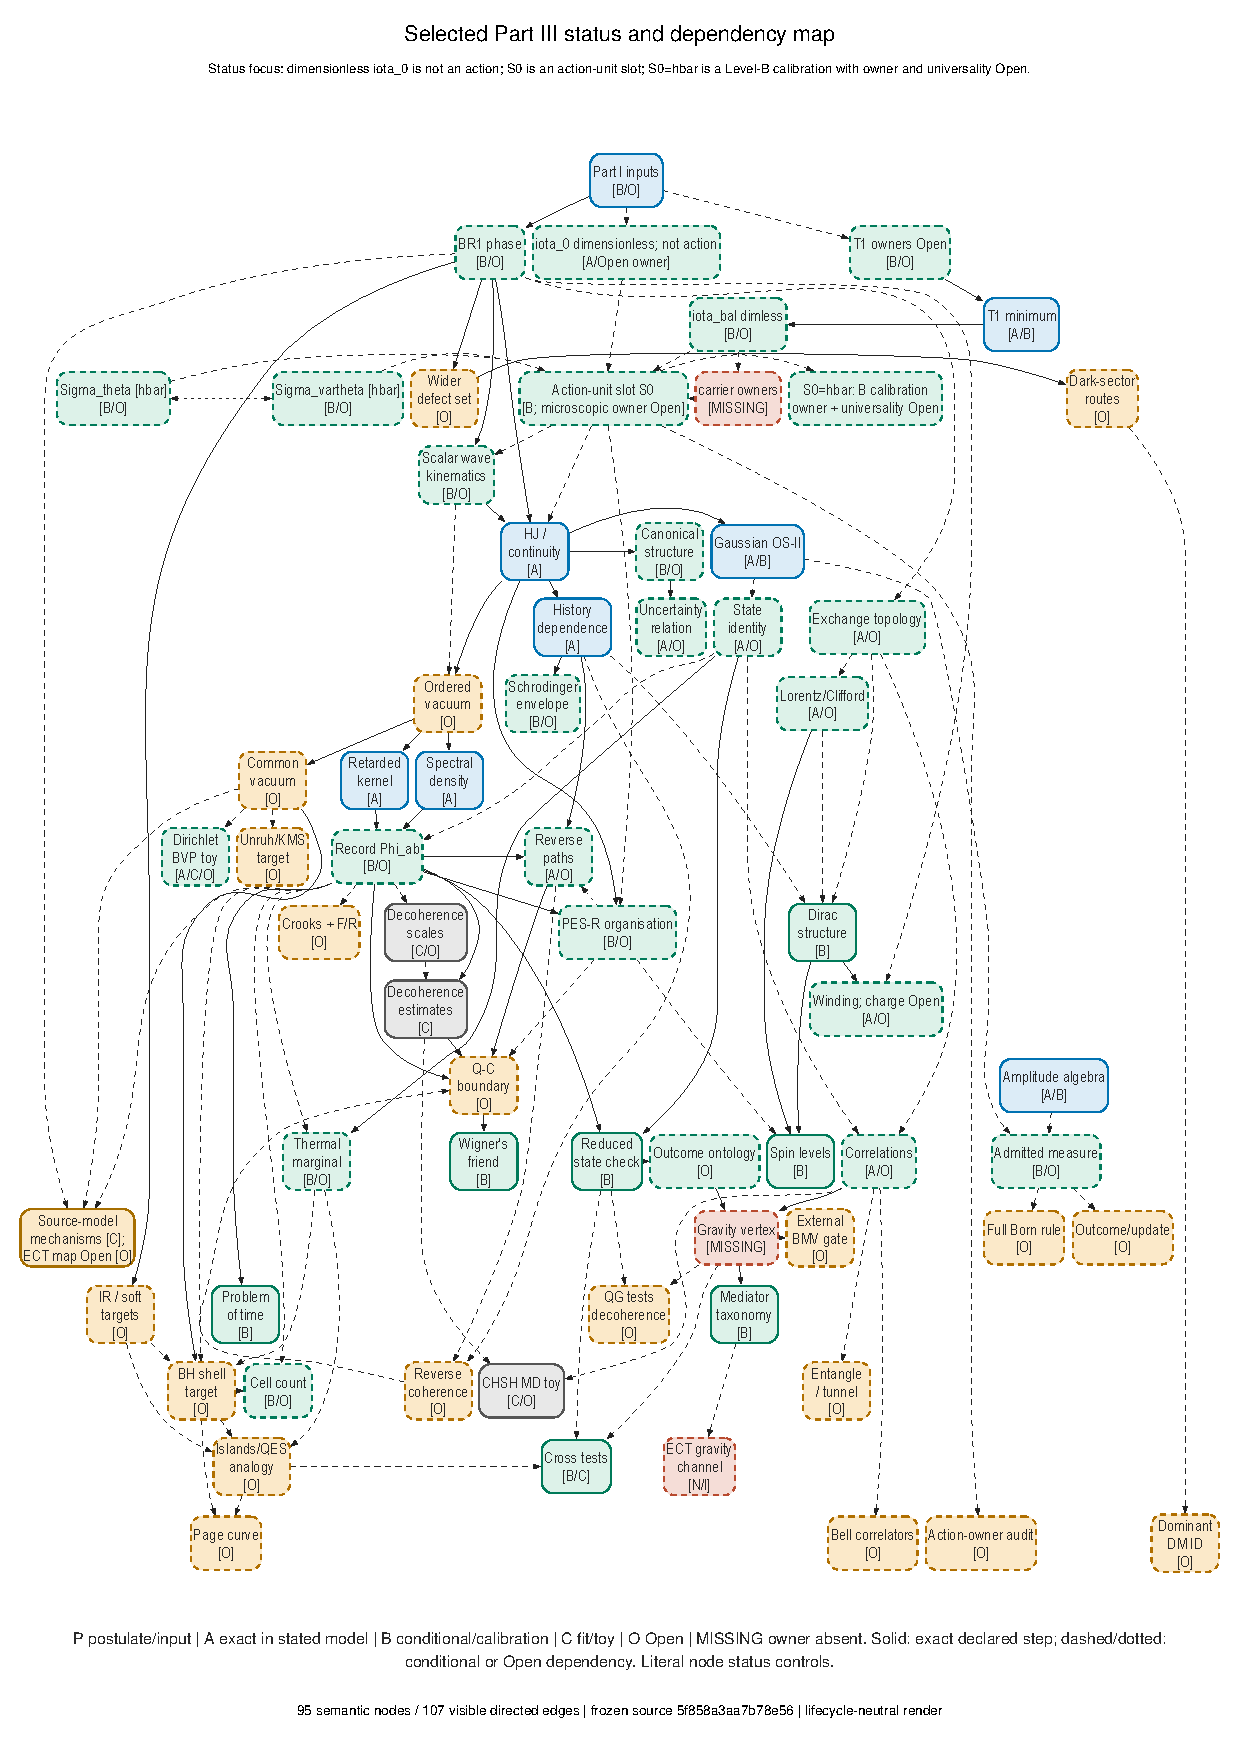
\includepdf[
  pages=1,
  pagecommand={\thispagestyle{empty}\phantomsection
    \refstepcounter{figure}
    \label{fig:qs_consistency}
    \label{app:r141_complete_part_iii_logic}
    \label{app:r129_visual_part_iii_logic}
    \label{appfig:r123_atlas_fig36}
    \label{appfig:r123_topology_fig36}
    \addcontentsline{lof}{figure}{\protect\numberline{\thefigure}Selected status and dependency map of Part~III}}
]{figures/r185/logic_maps/partIII_status_dependency.pdf}

\paragraph{Reading discipline.}
The poster uses the same status semantics as the other part maps: solid
arrows organise declared dependencies, dashed arrows show conditional/Open
links, and literal node text controls status.  T1 supplies neither
$S_0=\hbar$ nor a PES-selected occupation law.  The connected A4 map preserves
the full topology in a zoomable vector rendering; exact source, label and edge
records remain in its deterministic companion key.


\paragraph{Principle of Euclidean Stationarity as organising output.}
PES-R is a Level-B/Open taxonomy with three non-equivalent layers:
sector-specific dynamical admissibility, finite-time retention, and pairwise
record distinguishability.  It does not replace the sector equations, derive a
universal scalar bath, or supply Born weights and measurement outcomes.  The
physical ECT kernels and record operators remain OP-PES-1 record-channel inputs.

\paragraph{Open problems of the Quantum Sector.}
\begin{description}[leftmargin=2.2em]
  \item[OP-Q1] Derive or refute, from one 4D coherent-sector
    action and profile, the reduced stiffness $K_\theta^{1\mathrm D}$,
    positive line tension $\mathcal T_{\rm loop}$, unwinding barrier and
    backreaction entering the conditional balanced-loop route; then test
    whether its action scale is universal (Appendix~\ref{app:Sloop_calc}).
  \item[OP-Q2] Final identification of the pre-quantum action scale
    with the observed $\hbar$~\eqref{eq:qs_S0_identification}.
  \item[OP-Q3] Full derivation of the effective coherent Hamiltonian
    $\hat H_{\rm coh}$ for the relevant physical sectors.
  \item[OP-Q4] Rigorous derivation of quantum commutators from the
    coherent branch beyond canonical plausibility
    arguments~\eqref{eq:qs_commutator_candidate}.
  \item[OP-Q5] Derive the physical resolved/unresolved split,
    record operators, state, retarded kernel, and noise kernel entering
    Eq.~\eqref{eq:qs_influence}.
  \item[OP-Q6] Derivation of the effective ohmic regime and of the
    Markov limit from the condensate bath without auxiliary closure
    assumptions~\eqref{eq:qs_ohmic}.
  \item[OP-Q7] Full first-principles emergence of the Hilbert-space projector
    and probability-measure structure from bare P1--P6.  Complete applicable
    corrected OS-II packages close the standard Hilbert reconstruction only
    for supplied Gaussian broken-phase models~(Level~A mathematics); what
    remains includes the full interacting OS-II package~(OP-Q16), a physical
    state/preparation and event algebra, probability origin, record/dephasing
    channel, outcome and update.  Ordinary projector Gleason only represents
    an independently admitted measure in complex dimension at least three; a
    qubit requires the Busch effect/POVM theorem under separately declared C2q hypotheses.
  \item[OP-Q8] Completed measurement theory: branch update, pointer
    stability, and record formation.
  \item[OP-Q9] Dynamical classification, production, and stability of
    topological defect sectors outside the smooth coherent branch
    (Section~\ref{sec:qs_defects}).
  \item[OP-Q10] Quantitative link between coherent dark
    candidates and observed dark-sector phenomenology.
  \item[OP-Q11] Physical realisation of spinorial excitations in ECT
    and an explicit emergent many-excitation sector decomposition
    (Fock-like reconstruction) with variable excitation number from
    condensate dynamics.
    ECT does not require Fock space as a fundamental postulate, but
    the effective reconstruction---especially for the fermionic
    many-body sectors---remains to be constructed.
    Note: the abstract generator continuation and Clifford matrix
    algebra are Level~A conditional mathematics only after their metric and
    representation inputs are supplied; the restricted Dirac theorem is
    Level~B~(Section~\ref{sec:qs_dirac}).  The physical metric/spinor descent,
    excitation spectrum and CAR/Fock sector remain Open.
  \item[OP-Q12] Quantitative derivation of coherent-vacuum response
    effects (Casimir force, particle production rates, Unruh detector
    response) from the completed reduced coherent
    EFT~(Sections~\ref{sec:qs_casimir}--\ref{sec:qs_unruh}).
  \item[OP-Q12c] Thermal completion of the hot Big-Bang branch:
    entropy production, thermalisation, and radiation-bath
    formation after geometric branch onset; CMB acoustic-peak structure with cosmological matter content and
    matching left Open.
  \item[OP-Q12b] Derive or falsify a physical ECT owner for the
    conditional boundary-cell count, then test a covariant
    Bousso-type formulation for dynamical horizons and null
    hypersurfaces; full bulk--boundary reconstruction in the
    strong holographic sense remains Open.
  \Needspace*{6\baselineskip}
  \item[OP-Q13] Global nonlinear completion of the black-hole
    evaporation problem in the presence of a critical ordered-phase shell, including
    (i) explicit shell dynamics and profile,
    (ii) generalized-entropy evolution~\eqref{eq:qs_generalized_entropy},
    and (iii) a Page-curve-type computation for the reduced radiation
    sector~(Section~\ref{sec:qs_black_holes}).
  \item[OP-Q14] Construct an owner-complete strong-field action, state,
    solution, perturbation operators, radiation channel and likelihood;
    only then determine whether any nonzero compact-object or near-horizon
    observable differs from the external reference theory.
  \item[OP-Q15] Derive the physical ECT resolved/unresolved split,
    record operators, state, and spectral kernels, then determine whether any
    weak/strong monitoring interpolation exists.  Total mode count and an
    ohmic/Markov ansatz do not define a universal regime boundary.
  \item[OP-Q16] Construct the interacting coherent-sector Euclidean measure
    or Schwinger functions, physical observable algebra, and time reflection;
    verify temperedness together with the applicable OS-II regularity/growth
    condition (for example E0$'$ linear growth), Euclidean covariance, reflection positivity,
    permutation/graded symmetry, and all applicable locality and clustering
    requirements; then complete the Osterwalder--Schrader reconstruction and
    identify its time generator, clock/metric map, and supplied $S_0$ with the
    physical coherent branch.  Reflection positivity alone does not establish
    global unitarity beyond the quadratic regime.
  \item[OP-Q17] Construct an ECT reduced channel, state, entropy
    functional, and conditional entropy theorem; separately define
    forward/reverse protocols, path measures, time reversal, initial
    ensembles, and local detailed balance before testing a Crooks relation
    (Section~\ref{sec:crooks_ect}).
  \item[OP-Q18] Full quantitative Casimir derivation for the
    condensate-reflecting sector and identification of laboratory
    systems implementing the required ordered-medium boundary
    conditions~(Section~\ref{sec:qs_casimir}).
  \item[OP-Q19] Unique-outcome selection beyond conditional Born-rule
    weights, including the relation between branch weights,
    decohered alternatives, and actually realised measurement
    records~(Section~\ref{sec:qs_born}).
  \item[OP-Q20] Construct the physical Bell experiment from condensate
    dynamics: derive the preparation, physical state-or-configuration owner,
    setting generators, measurement maps and full joint outcome law.  If a
    hidden/configuration representation is proposed, also define its
    constrained space, positive measure, response/record maps and
    causal/intervention semantics, and determine rather than assume whether
    measurement independence or Bell factorisability fails.  In every route,
    derive the angular correlation law, operational no-signalling and the
    Tsirelson restriction, and test robustness across detector,
    random-generator and cosmic-setting protocols
    (Section~\ref{sec:qs_entanglement}).
  \item[OP-Q21] Smooth-branch exactness of the Pauli exclusion
    principle and its admissible departures. Determine whether the
    completed fermionic reconstruction of ECT enforces exact
    canonical anticommutation relations throughout the smooth
    coherent ordered branch, as provisionally indicated by the
    canonical-normalisation no-go argument of
    Section~\ref{sec:qs_statistics} and
    Appendix~\ref{app:pauli_exactness}. If genuine departures from
    standard fermionic statistics exist in ECT, identify the
    precise nonlocal, topological-defect, or branch-transition
    mechanism responsible, rather than attributing them to smooth
    local condensate gradients.

  \medskip
  \textbf{PES-R-specific open targets}
  (\S\ref{sec:pes_open}):
  \item[OP-PES-1] Derive the physical resolved/unresolved split, record
    operators, and ECT retarded/noise kernels from the action.
  \item[OP-PES-2] Derive, or rule out, a one-history large-deviation/path
    measure with its drift, diffusion, Jacobian, convention, and boundaries.
  \item[OP-PES-3] Complete the physical graviton sector and UV closure;
    PES-R itself is not a quantisation prescription.
  \item[OP-PES-4] Derive physical decay widths from vertices, self-energies,
    form factors, states, and phase space.
  \item[OP-PES-5] Test whether any backreaction map connects a reduced-state
    record exponent to $\alpha-\beta$; no such map is currently known.
  \item[OP-PES-6] Generalise the toy information--dephasing relation to a
    specified detector channel; no protocol-independent bound is claimed.
  \item[OP-PES-7] Construct one action-owned, constraint-reduced physical
    channel in which retarded response and ordered noise are measured with the
    same operator, source vertex, projector, form factor, state and detector
    transfer.  Apply the Wightman inequalities first and then test a
    preregistered single-temperature KMS model on held-out frequency bins.
  \item[OP-PES-8] Derive a gauge-invariant primordial record operator, state
    and generally two-time ordering-front kernel; propagate its declared
    phase-diffusion or mode-mixing template through the Boltzmann/recombination
    map before using acoustic phase data.  The CMB does not directly identify
    $\Phi_{ab}$ or a pointer basis.

\medskip
\noindent\textbf{Frozen P6 record-sector open targets}
(Appendices~\ref{app:AP6A-conventions-kernels}--\ref{app:AP6H-honesty-correction-index}).
\item[OP-P6-1] Per-protocol selection of the effective record-temperature
  source $T_{\rm eff}$ for the M3 implementations (frozen-ledger
  register O2).
\item[OP-P6-2] Unresolved record/line-ensemble entropy matching in the P6
  sector.  The frozen ledger uses the shorthand $s_{\rm unres}/\mu$
  for the open problem of defining whether unresolved record
  degeneracy should be represented by a coarse-grained entropy density
  $s_{\rm unres}$, by a line/path multiplicity $\mu$, or by a
  protocol-specific entropy factor.  Any such term must be defined at
  a declared core scale and compared with the pair pressure
  $\sigma_{\rm dec}$; it is not an adjustable stabilising entropy.
\end{description}

The common technical object unifying OP-PES-1, OP-PES-2, OP-PES-4,
and the quantitative side of OP-PES-6 is the condensate spectral
density $J(\omega,\mathbf{x})$: one kernel fixes decoherence,
dissipation, decay widths, lifetimes, and the quietness index.

\subsection{Status-separated minimal quantum reconstruction core}
\label{sec:qs_minimal_core}

The following results organise the minimal quantum core of ECT into
three layers: a strict structural core, a structurally singled-out
backbone, and the nearest closure-level or open fronts.
They should be read together with the detailed status map in
Section~\ref{sec:qs_status}: the purpose of the present subsection is
not to replace the full table, but to identify the irreducible
backbone that already exists inside the theory and to separate it
clearly from what still depends on closure or remains open.

\paragraph{Status-separated mathematical core.}
\begin{enumerate}[label=(\roman*)]
  \item Integer winding classification is Level~A topology only within the
    supplied compact-$U(1)$ phase EFT.
  \item Conditional Madelung decomposition after a norm-preserving complex
    evolution law, Hamiltonian, domain and clock convention are supplied;
    ECT ownership of those inputs is Open.
  \item Poisson-bracket organisation is classical conditional mathematics;
    a physical canonical quantum representation remains Open.
  \item Discreteness of the integrated compact-phase generator follows only
    after its representation is supplied; the physical generator and its
    $S_0$ normalisation are Open.
  \item The Robertson--Schr\"odinger inequality is Level~A mathematics only
    after a Hilbert space, self-adjoint domains and commutator are supplied;
    the physical commutator and coefficient $S_0$ remain Level~B/Open.
  \item Reflection positivity and standard OS reconstruction in the supplied
    free Gaussian scalar models under their complete declared hypotheses
    (massive radial and free massless Goldstone-coordinate measures); physical
    ECT mode identification remains Open.
  \item The structural distinction between global and reduced
    unitarity.
  \item Two-sided Euclidean boundary dependence from the elliptic
    field equation.
  \item Exchange-sector topology
    $\pi_1(\mathcal{M}_2)=\mathbb{Z}_2$ in the separately supplied
    defect-free $\mathbb R^3$ point-configuration model; its physical slice
    and excitation map remain Open.
  \item Standard Lorentz-generator and Clifford matrix algebra after
    the complex continuation, metric and spinor representation are supplied;
    their physical ECT owners remain Open.
  \item Retarded propagation of the supplied quadratic ordered-branch scalar,
    together with the exact conditional hyperbolicity gate for a declared
    $P(X)$ branch and nonnegative spectral density in the quadratic sector.
  \item Structural admissibility of reverse
    $O(3)\!\to\!O(4)$ Euclidean segments in the path integral.
  \item The amplitude / decoherence / probability distinction.
  \item A future globally unitary interacting completion would exclude
    fundamental information destruction; P1--P6 do not yet prove that
    completion.
  \item The ordered-condensate state space is not exhausted by the smooth
    coherent branch~BR1.
\end{enumerate}

\paragraph{Structurally singled-out backbone (Level~A/B).}
\begin{enumerate}[label=(\roman*)]
  \item The presence of two supplied loop-scale candidates,
    $\iota_0^{\rm EFT}$ and $\iota_{0,\rm bal}^{\rm eff}$, together with an Open
    programme for deriving their common four-dimensional owner, selecting a
    viable route and mapping the corresponding action-valued product
    $\Sigma_\theta\iota_0$ to operational $S_0$, and testing universality.
  \item The unified vacuum-response logic relating Casimir, Unruh,
    particle production, and horizon thermality as four probing
    regimes of one coherent vacuum.
  \item Named laboratory source models realise compact phase, winding,
    response and decoherence mechanisms.  These external results motivate
    controlled bridge-building, but are not evidence for ECT; an ECT test
    remains Open until the six-owner bridge and discriminator are supplied.
\end{enumerate}


\paragraph{Closure-level results and open fronts (Level~B / Open).}
\begin{enumerate}[label=(\roman*)]
  \item Generic influence-functional and reduced-state mathematics is
  available, but the ECT environment split, record operators, kernels, state,
  and entropy-production theorem remain Open.
  \item C$_{60}$, Fein and Pedalino observations are external
  environmental-decoherence anchors; the apparatus rates are not reproduced
  here.  The Di\'osi--Penrose functional and declared hard-sphere
  orientation point are external comparisons, not an ECT rate.
  \item Visibility losses define dephasing proxies in declared simple models;
    they are neither ECT kernel determinations nor reverse-path probabilities.
  \item A common ordered medium supplies a candidate arena for correlated
    subsystems, but no nonfactorisation theorem, Bell measure or physical
    correlation law follows from common support; those owners remain Open.
  \item The qubit information--dephasing and CHSH calculations are toy-model
  thresholds, not universal quantum--classical or measurement theorems.
  \item Born-type weights have a conditional trace representation only after
  (C1)--(C2), with (C3) needed for a physical application and an explicit
  extension needed in dimension two; the physical measure and unique outcome
  remain Open.
  \item PES-R organises modes already supplied by the sector dynamics; its
  one-history, signature-changing, lifetime, and universal-selection readings
  are not derived and remain Open.
  \item Full interacting OS closure, spin--statistics, Bell correlators,
  condensate-reflecting Casimir response, nonperturbative evaporation, defect
  dominance, and the microscopic value of $S_0$ remain their named Open tasks.
\end{enumerate}

This distinction is essential.
ECT does not yet claim to have derived all of standard quantum
mechanics from its postulates.
What has been identified is a dependency map: supplied scalar/coherent models
host several exact mathematical substructures, while physical quantum states,
operators, probability, outcomes, entanglement channels and strong-field
owners remain explicitly separated Open tasks.


\paragraph{Mesoscopic gravity owner firewall.}
The external Di\'osi--Penrose functional supplies no ECT-specific rate or
correction.  An application requires its own density profile and
regularisation, while an ECT claim additionally requires the record vertex,
state, noise kernel, and finite-body charge.

\paragraph{Logical relocation of quantum mechanics.}
Part~III reconstructs several kinematic ingredients and states explicit Open
targets.  A complete applicable corrected OS-II package governs the separate
Hilbert reconstruction.  Independently, ordinary projector Gleason represents
only an already supplied normalised, noncontextual, countably additive
projector measure in complex dimension at least three, with the Busch effect/POVM theorem under separately declared C2q hypotheses required for a qubit.
State/preparation, event, probability origin, outcome and update remain Open;
decoherence explains reduced-state interference suppression but does not
create those owners, and PES-R is an organising taxonomy rather than their
derivation.

\subsection{ECT as a foundational framework for quantum mechanics:
structural comparison with the standard formalism}
\label{sec:qm_capstone}
% ==============================================================

\textit{Status: comparative and pedagogical synthesis of results
established in the preceding sections of Part~III.  No new physical
results are introduced here.  The role of this subsection is to
organise the structural comparison between ECT and the standard
quantum formalism along three explicit axes: ontology of the
primary object, type of mathematical problem, and origin of the
statistical description.  The formal status ledger of the same
material, organised by derivational level and keyed to the
open-problem labels, is given separately in
Section~\ref{sec:qs_minimal_core}; current limitations of the
formulation are collected in Section~\ref{sec:limitations}.}

Standard quantum mechanics is an extraordinarily successful predictive
formalism.  Part~III asks whether selected pieces of that formalism can be
reconstructed conditionally from a Euclidean condensate model.  The answer is
status-separated: the bare Euclidean equation and some linear/Gaussian
identities are Level~A inside their stated models; the scalar Lorentzian and
Schr\"odinger-type reductions are conditional; and the physical Hilbert-space
map, operator algebra, universal action scale, probability measure, outcomes,
particle statistics, and detector channels remain Open.  The comparison below
therefore organises a reconstruction programme.  It does not claim that ECT
already explains why the full quantum formalism is realised in nature.

% ------------------------------------------------------------------
\subsubsection*{Two different questions answered by two theories}
\label{sec:qm_capstone_two_questions}
% ------------------------------------------------------------------

Standard quantum mechanics supplies the tested operational rules.  ECT treats
some of those rules as possible reconstruction targets.  Table~\ref{tab:qm_capstone_two_questions}
distinguishes what is part of the present ECT input, what has been obtained
conditionally, and what still lacks an owner.

{\small
\renewcommand{\arraystretch}{1.25}
\begin{longtable}{@{}L{3.6cm}L{5.8cm}L{5.7cm}@{}}
\caption{Two questions, two frameworks.  Each row records the
fundamental ingredient on which the two theories differ at the
architectural level; detailed cross-references to Part~III are
given in the concept-mapping
Table~\ref{tab:qm_capstone_concept_mapping} below.}
\label{tab:qm_capstone_two_questions}\\
\toprule
Aspect & Standard quantum mechanics & Euclidean Condensate Theory \\
\midrule
\endfirsthead
\toprule
Aspect & Standard quantum mechanics & Euclidean Condensate Theory \\
\midrule
\endhead
\midrule
\endfoot
\bottomrule
\endlastfoot
Primary question & How to compute observed outcomes efficiently
  & Can specified quantum structures be reconstructed from a supplied
    Euclidean-medium model? \\
Status of axioms & Foundational postulates (Hilbert space, Born
  rule, canonical commutators)
  & Reconstruction targets; most physical owners remain Open \\
Primary physical object & Complex amplitude $\psi(x,t)$
  & Real scalar field $\Phi(X)$ in the bare model; its physical state map is
    an additional matching problem \\
Arena & $3{+}1$ Lorentzian spacetime, assumed as background
  & $4$D Euclidean manifold; a scalar Poincar\'e-form principal operator is
    conditional on supplied P4 background/EFT data \\
Role of time & Fundamental external parameter
  & A candidate real parameter $x^0=w$ exists on the supplied ordered branch;
    physical clocks and time observables remain Open \\
Role of causal speed & Speed of light postulated
  & The dimensionless scalar ratio
    $\hat c_*^2=\beta/(\alpha-\beta)$ follows conditionally;
    $c_{\rm char}=c$ is the adopted Level-B scalar-clock calibration after the
    unit/lapse map, while photon, matter and tensor cone equality remains Open \\
Role of $\hbar$ & Fundamental universal constant
  & Two supplied loop closures carry distinct candidates; neither owns
    the operational $S_0$, and compactness alone fixes neither a nonzero
    universal microscopic owner; $S_0=\hbar$ is instead the adopted
    Level-B calibration
    (see \S\ref{sec:qs_hbar}) \\
Role of probability & Primitive (Born rule)
  & Probability measure and outcome law remain Open; tracing and decoherence
    do not create either \\
Causal structure & Built in from the start
  & Scalar characteristic cone conditional on P4/EFT inputs; physical causal
    structure remains a completion target \\
Type of mathematical problem & Forward-time Cauchy problem for
  amplitude
  & Elliptic boundary-value problem for the bare scalar; the quantum state,
    preparation and detector map remain Open \\
\end{longtable}
}

The table is a dependency map, not evidence that the reconstruction has been
completed.  Standard quantum mechanics remains the empirical calculational
theory against which every proposed ECT owner must be tested.

% ------------------------------------------------------------------
\subsubsection*{Hierarchy of effective equations}
\label{sec:qm_capstone_hierarchy}
% ------------------------------------------------------------------

Figure~\ref{fig:equation_hierarchy} and
Table~\ref{tab:qm_capstone_hierarchy} show a \emph{candidate reduction
chain}.  Its arrows do not all have the same status: Level~0 is the bare model,
P4 supplies rather than derives the ordered branch used at Level~1, the scalar
Klein--Gordon form is a conditional principal-operator result, and the
Schr\"odinger endpoint additionally requires a state space, operator
normalisation and a supplied $S_0$.

\paragraph{Level~0: Euclidean condensate equation.}
At the most fundamental level one has the Euclidean field equation
\begin{equation}
  \label{eq:ect_euclidean_fundamental}
  \delta^{AB}\partial_A\partial_B \Phi - V'(\Phi)=0,
\end{equation}
which is the Euler--Lagrange equation of the bare Euclidean
micro-action~\eqref{eq:ECT_action}; it is written here only to
display the logical hierarchy, not as a new independent postulate.
It is a four-dimensional elliptic equation for the condensate field
$\Phi$.  At this level there is no distinguished time coordinate, no
$\hbar$, and no built-in probabilistic interpretation.  All four
coordinates are spatial from the Euclidean point of view.  Boundary data
specify the problem on the full four-dimensional domain, but determine a
unique solution only after existence, uniqueness and stability/well-posedness
are proved for the stated nonlinear equation, domain and boundary class;
these global properties remain Open.

\paragraph{Level~1: adopted P4 branch plus a separately supplied scalar EFT.}
P4 postulates the physically relevant nonzero-gradient branch and supplies
its directional chart; its $O(3)$ stabiliser is exact conditional mathematics.  If a scalar kinetic EFT, the coefficients $\alpha,\beta$
and the effective mass input are additionally supplied, the relevant
fluctuation equation takes the form
\begin{equation}
  \label{eq:ect_ordered_branch_wave}
  K^{AB}\partial_A\partial_B\chi + m_{\rm eff}^2\chi = 0.
\end{equation}
Within the restricted parity-even, two-derivative scalar principal-symbol
basis built only from $\delta^{AB}$ and the supplied director $n^A$, the
general symmetric tensor has the form
\begin{equation}
  K^{AB}=\beta\,\delta^{AB}-\alpha\,n^A n^B.
\end{equation}
This basis-level classification is conditional on that operator inventory;
P4 neither derives the scalar EFT nor fixes $\alpha$, $\beta$ or
$m_{\rm eff}$ (see Eq.~\eqref{eq:ordered_branch_euclidean_eft} and the
subsequent scoped uniqueness discussion).  For a homogeneous background with
$n^A=\delta^A_w$, this gives
$K^{AB}=\mathrm{diag}(\beta,\beta,\beta,\beta-\alpha)$,
so that the Lorentzian regime is controlled by the sign of
$\beta-\alpha$, equivalently by
\begin{equation}
  \hat c_*^2=\frac{\beta}{\alpha-\beta}.
\end{equation}
Thus, on the declared $\beta>0$ branch, $\alpha>\beta>0$ gives a
Poincar\'e-form scalar principal operator, $\alpha<\beta$ gives an elliptic
operator, and $\alpha=\beta$ is singular.  Without $\beta>0$, the full product
criterion must be used.  This is a conditional statement about the
scalar characteristic operator, not a derivation of physical clocks, photons,
rods, tensor gravity or quantum kinematics.

\paragraph{Level~2: relativistic Lorentzian wave equation.}
For the supplied ordered branch with $\alpha>\beta>0$ on the retained
$\beta>0$ component, after the real
parametrisation $x^0=w$, the fluctuation equation takes the
relativistic Klein--Gordon form~\eqref{eq:KG}
(see Section~\ref{sec:qs_wave_kinematics} for the derivation).
A separate formal continuation $w_E \to \pm i\,t$ may still be
used when relating Euclidean coherent amplitudes to Lorentzian
phase evolution; the first step is a scalar-coordinate
reparametrisation in the ordered branch, while the second is only a
translation of Euclidean coherent amplitudes into Lorentzian phase
language.

\paragraph{Level~3: conditional nonrelativistic Schr\"odinger-type limit.}
Given a compatible complex state representation, a supplied action scale and
the usual positive-frequency/nonrelativistic assumptions, extraction of the
rest-energy phase $\psi = e^{-im c_{\rm char}^2 t/S_0}\chi$ and neglect of
terms of order $v^2/c_{\rm char}^2$ give the Schr\"odinger-type
coherent equation~\eqref{eq:qs_schrodinger_type}.  Its identification with
the standard Schr\"odinger equation of textbook quantum mechanics remains a
Level-B/Open reconstruction step
(see~\S\ref{sec:qs_wave}).  The displayed equation is therefore a
conditional endpoint, not an already-derived physical quantum sector.

\begin{figure}[tbp]
\centering
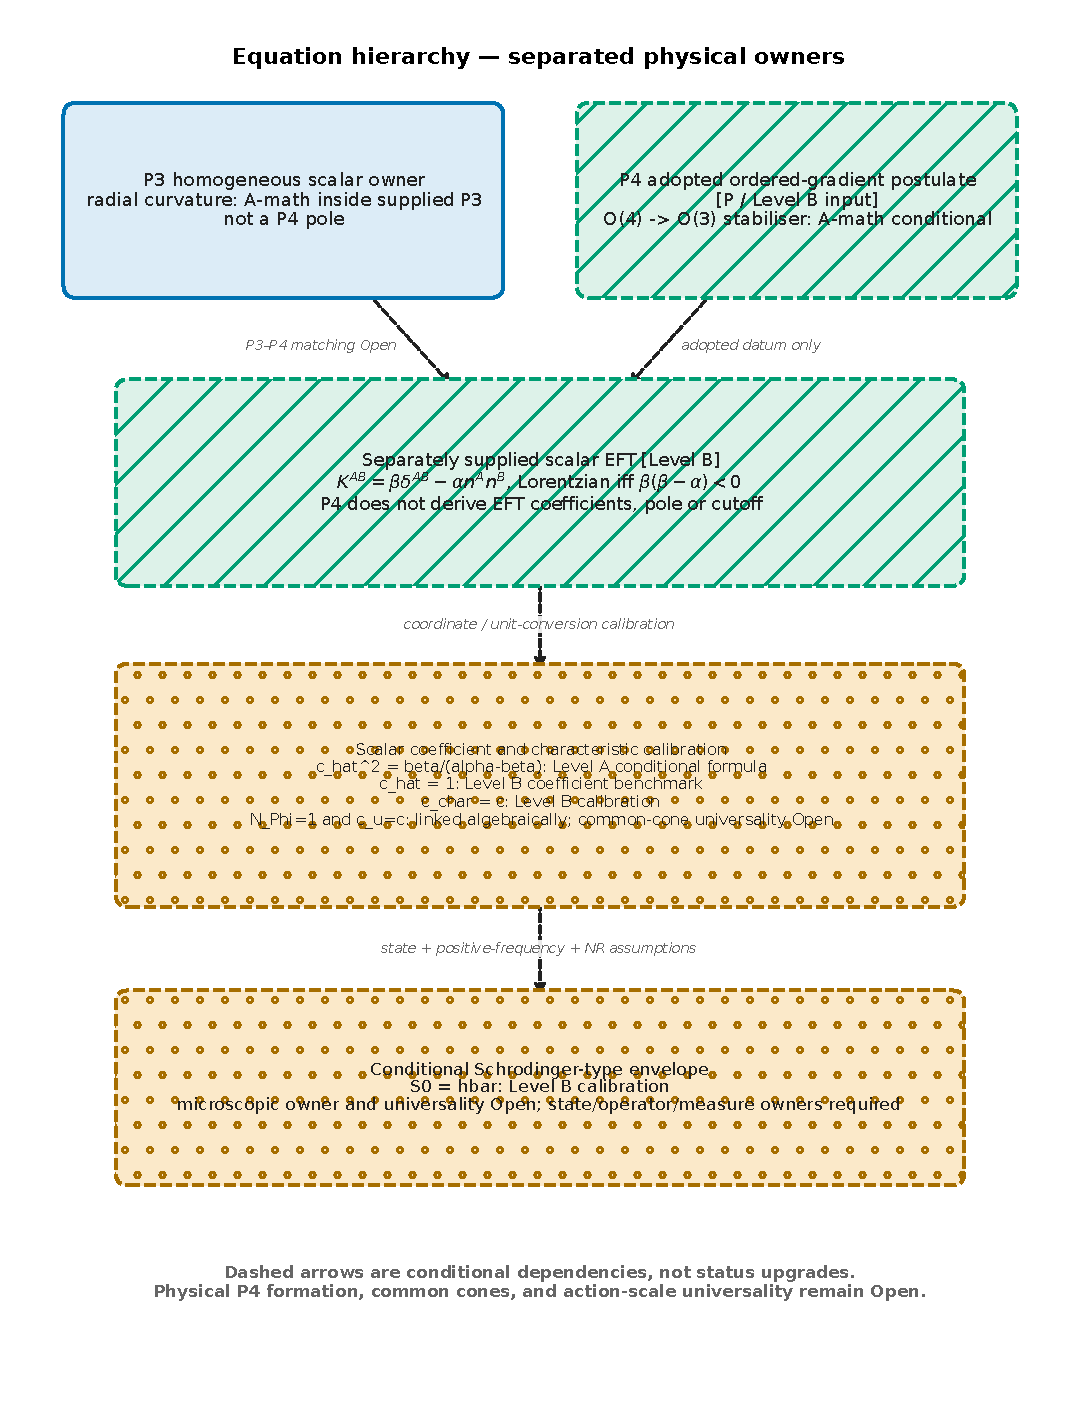
\includegraphics[width=0.95\textwidth]{figures/r177/global/fig_equation_hierarchy_r177.pdf}
\caption{Status-separated candidate hierarchy.  Level~0 is the supplied bare
Euclidean scalar model; P4 supplies the ordered background/EFT used at
Level~1; Level~2 is a conditional scalar Klein--Gordon-form reduction; and
Level~3 additionally assumes the state/operator/$S_0$ data required for a
Schr\"odinger-type equation.  Layout arrows are organisational, not status
upgrades.  No arrow by itself derives a physical clock, Hilbert space, Born
measure or detector channel.}
\label{fig:equation_hierarchy}
\end{figure}

{\small
\renewcommand{\arraystretch}{1.25}
\begin{longtable}{@{}C{0.05\linewidth}L{0.21\linewidth}L{0.15\linewidth}L{0.15\linewidth}L{0.15\linewidth}L{0.158\linewidth}@{}}
\caption{Hierarchy of effective equations in ECT, together with
the type of problem they define, the data needed to solve them, and
their standard-QM counterpart.}
\label{tab:qm_capstone_hierarchy}\\
\toprule
Lv. & Equation & Regime & Mathematical type & Data &
  Standard-QM analogue \\
\midrule
\endfirsthead
\toprule
Lv. & Equation & Regime & Mathematical type & Data &
  Standard-QM analogue \\
\midrule
\endhead
\midrule
\endfoot
\bottomrule
\endlastfoot
0 & $\delta^{AB}\partial_A\partial_B\Phi=V'(\Phi)$
  & P3 Euclidean regime before the supplied P4 datum
  & Elliptic
  & Global BVP on $\partial\mathcal{M}$
  & none \\
1 & $K^{AB}\partial_A\partial_B\chi+m_{\rm eff}^2\chi=0$,
    $K^{AB}=\beta\delta^{AB}-\alpha n^A n^B$
  & P4 directional datum plus a separately supplied scalar EFT and
    coefficient branch
  & On the declared $\beta>0$ branch: elliptic for
    $\alpha<\beta$, hyperbolic for $\alpha>\beta>0$; in general the
    Lorentzian criterion is $\beta(\beta-\alpha)<0$
  & BVP or IVP depending on the supplied coefficient branch
  & none \\
2 & $(\Box-m^2)\chi=0$, $x^0=w$
  & Conditional scalar Poincar\'e-form branch
    ($\alpha>\beta>0$ on the retained $\beta>0$ component)
  & Hyperbolic
  & Cauchy data on $t=\mathrm{const}$
  & Klein--Gordon \\
3 & $iS_0\,\partial_t\psi=H\psi$
  & Conditional state/operator/$S_0$ completion and nonrelativistic limit
  & Parabolic/\allowbreak effective
  & Cauchy data at $t=0$
  & Schr\"odinger-type sector \\
\end{longtable}
}

% ------------------------------------------------------------------
\subsubsection*{What the ordered-branch equation contains beyond
Schr\"odinger}
\label{sec:qm_capstone_beyond_schr}
% ------------------------------------------------------------------

The supplied ordered-branch equation~\eqref{eq:ect_ordered_branch_wave}
contains more scalar-EFT structure than the conditional Schr\"odinger-type
endpoint~\eqref{eq:qs_schrodinger_type}.  The comparison below separates
algebraic facts from missing physical ownership.

\begin{enumerate}[label=(\roman*)]
\item \emph{Both signatures in one equation.}  On the declared $\beta>0$
component, for $\alpha<\beta$,
the effective equation remains elliptic and describes the Euclidean
coherent sector, where there is no causal ordering and solutions
depend on boundary data from the full domain.  For $\alpha>\beta>0$,
the equation becomes hyperbolic and supports causal propagation.
The Schr\"odinger-type endpoint addresses only the selected hyperbolic scalar
branch and only after additional nonrelativistic/state assumptions.
\item \emph{Relativistic parent.}  Level~2 is manifestly a
Klein--Gordon-type relativistic sector, not a nonrelativistic
residue.  The nonrelativistic limit appears only at Level~3.
\item \emph{Scalar slope and physical calibration.}  The principal
operator fixes the dimensionless
$\hat c_*^2=\beta/(\alpha-\beta)$ inside the supplied scalar EFT.  It cannot be
equated to a speed.  The separate equality $c_{\rm char}=c$ is the adopted
Level-B scalar-clock calibration after the unit/lapse map; photon, matter and
tensor cone equality remains Open.
\item \emph{Candidate loop scales and operational slot.}  The supplied
fixed-core phase-gradient functional defines $\iota_0^{\rm EFT}$ by evaluation at
$L_{\rm core}$, while the supplied positive-tension model defines
$\iota_{0,\rm bal}^{\rm eff}$ by minimisation (Section~\ref{sec:qs_hbar}).
Winding supplies the integer label only.  A relation such as
$\oint dw\,p_w=2\pi nS_0$ additionally requires an independently derived
canonical pair or action--angle map; it does not follow from compactness.
Neither route maps itself to operational $S_0$, the operator algebra, or
$S_0=\hbar$.
\item \emph{Separate gravity completion.}  The scalar ordered background is a
possible common input to coherent and geometric completion programmes, but the
current scalar action does not derive an independent helicity-2 mode, Newton's
constant, a physical metric, or their backreaction on the quantum state.
\item \emph{Status-separated structural programme.}  The
ordered-branch equation is compatible with two-sided Euclidean boundary
dependence and with constructing declared reduced-state record channels.
It does not derive a metric-signature transition, physical reverse
$O(3)\!\to\!O(4)$ segments, one unique outcome, or a common dynamical
mechanism for entanglement and tunnelling.  The gravitational record
projector, state, noise kernel, and rate remain Open.
\end{enumerate}

The upshot is limited but useful: the supplied scalar EFT admits a conditional
KG-to-Schr\"odinger reduction chain.  Establishing that this chain is the
physical quantum sector, and coupling it consistently to a completed metric
sector, remain Open.

% ------------------------------------------------------------------
\subsubsection*{Ontological comparison: $\Phi$ versus $\psi$}
\label{sec:qm_capstone_ontology}
% ------------------------------------------------------------------

Standard quantum mechanics formulates predictions with states and amplitudes.
The ECT bare model instead begins with a real scalar $\Phi(X)$ on a Euclidean
domain.  Calling that scalar the physical medium is a defining ontology of the
framework, whereas deriving the quantum state, probability and detector maps
from it is an Open dynamical problem.  Table~\ref{tab:qm_capstone_ontology}
keeps those two statements separate.

{\small
\renewcommand{\arraystretch}{1.25}
\begin{longtable}{@{}L{3.9cm}L{5.6cm}L{5.6cm}@{}}
\caption{Ontological status of the primary object in the two
frameworks.}
\label{tab:qm_capstone_ontology}\\
\toprule
Aspect & $\psi$ in standard QM & $\Phi$ in ECT \\
\midrule
\endfirsthead
\toprule
Aspect & $\psi$ in standard QM & $\Phi$ in ECT \\
\midrule
\endhead
\midrule
\endfoot
\bottomrule
\endlastfoot
Type of object & Complex-valued amplitude
  & Real scalar condensate field \\
Physical interpretation & Not a physical field on spacetime;
  a mathematical object used to compute probabilities
  & Candidate physical medium variable by ECT definition; quantum-state and
    observable ownership Open \\
Arena & $3{+}1$ Lorentzian spacetime, taken as a background
  & $4$D Euclidean manifold; scalar hyperbolic principal form is conditional,
    while a physical spacetime metric remains Open \\
Role of time & Explicit parameter in the evolution equation
  & Absent at Level~0; $x^0=w$ is a conditional scalar coordinate and physical
    clocks remain Open \\
How it is fixed & Initial data at $t=0$, evolved forward
  & Boundary data on $\partial\mathcal{M}$ in the full 4D domain \\
Role in measurement & Supports the standard measurement/update formalism
  & Reduced-state dephasing is available for supplied channels; pointer basis,
    outcome and update rule remain Open \\
Access by observer & Direct calculational object
  & Full condensate configuration is rarely accessible;
    subsystem access only \\
\end{longtable}
}

Formally, the key statement is:

\begin{quote}
\emph{Standard quantum mechanics uses a state/amplitude as its primary formal
object.  ECT posits a real Euclidean scalar medium as its primary model object.
A derivation of the physical quantum state, probability measure and detector
map from that scalar has not yet been completed.}
\end{quote}

The remaining question is therefore not whether one can rename standard
quantum concepts in medium language, but whether explicit state, operator,
probability and detector maps can be derived and tested.

% ------------------------------------------------------------------
\subsubsection*{Epistemological comparison: boundary-value versus
Cauchy problem}
\label{sec:qm_capstone_epistemology}
% ------------------------------------------------------------------

The bare Euclidean scalar equation is naturally posed as a boundary-value
problem, whereas standard Lorentzian quantum equations are normally posed with
state/initial data.  This mathematical contrast is exact at the level of the
specified equations, but it does not prove uniqueness of the nonlinear
Euclidean boundary-value problem or identify its boundary data with laboratory
state preparation and readout.  Table~\ref{tab:qm_capstone_bvp_vs_cauchy}
summarises the conditional comparison.

{\small
\renewcommand{\arraystretch}{1.25}
\begin{longtable}{@{}L{3.6cm}L{5.8cm}L{5.7cm}@{}}
\caption{Boundary-value versus Cauchy description of quantum
dynamics in ECT and standard quantum mechanics.}
\label{tab:qm_capstone_bvp_vs_cauchy}\\
\toprule
Aspect & Standard quantum mechanics & Euclidean Condensate Theory \\
\midrule
\endfirsthead
\toprule
Aspect & Standard quantum mechanics & Euclidean Condensate Theory \\
\midrule
\endhead
\midrule
\endfoot
\bottomrule
\endlastfoot
Mathematical type & Parabolic Schr\"odinger equation; hyperbolic
  Klein--Gordon equation
  & Elliptic Euclidean condensate equation
    (Level~0); signature switches within Level~1 \\
Problem type & Cauchy initial-value problem
  & Global boundary-value problem \\
Data & Initial amplitude $\psi(x,0)$
  & Boundary data on $\partial\mathcal{M}$ \\
Domain & $3{+}1$ spacetime, evolved forward in $t$
  & Full $4$D Euclidean manifold, solved globally \\
Notion of determinism & Unitary forward evolution of a supplied state
  & A solution is fixed only when a well-posed/unique Euclidean BVP is supplied;
    uniqueness is not automatic \\
What counts as prediction & Probabilities from the standard state and Born rule
  & Requires an as-yet Open map from $\Phi$ and boundary data to physical
    preparations, observables and probabilities \\
Why probabilities appear & Postulated (Born rule) as an axiom
  & Not yet derived; coarse graining yields reduced states/dephasing but not an
    additive probability measure or outcome law \\
Role of future boundary data & None (initial-value problem)
  & Boundary data on all of $\partial\mathcal M$ enter a declared elliptic BVP;
    their physical preparation meaning is Open \\
\end{longtable}
}

Several consequences follow from this difference.

\paragraph{Probability remains a separate owner problem.}
For a declared system--environment split, integrating out untracked modes
produces an influence functional and can suppress reduced-state coherences
(Section~\ref{sec:influence_functional}).  This operation presupposes a state
and trace; it does not create an additive probability measure, the Born rule or
one realised outcome.  Those objects remain Open independently of the number
of untracked modes.

\paragraph{What reduced dynamics establishes.}
The detector belongs to the full system.  After a declared split and
coarse graining, a specified reduced channel can suppress off-diagonal terms
and form robust records.  This does not fix one realised outcome, derive a
pointer basis or update rule, or produce a Euclidean-to-Lorentzian
metric-signature transition.  Those detector-level objects remain Open
(OP-Q19).

\paragraph{Conditional global boundary sensitivity; no causal classification.}
In a supplied well-posed elliptic BVP, a change of admissible boundary data
can alter the global solution.  In a Lorentzian slicing this may resemble
two-sided conditioning, but it does not classify ECT as retrocausal or derive
delayed-choice statistics.  A physical conclusion would require the missing
well-posed solution map, preparation and setting generators, state, detector
map and Lorentzian causal structure.  Until those owners are supplied, the
causal class is \texttt{NOT IDENTIFIABLE} and no retrocausal signalling claim
is made.

\paragraph{BVP determination is not a Born derivation.}
Even a unique deterministic solution of a fully specified Euclidean BVP would
not by itself determine how an observer prepares a quantum state, assigns
probabilities or records one outcome.  Practical inaccessibility and
coarse-graining may motivate statistical modelling, but epistemic ignorance is
not a theorem establishing the Born measure.  The BVP, reduced-state and
probability questions must therefore remain distinct.

\paragraph{Candidate configuration-ensemble reading (Open).}
One possible but presently unclosed ECT interpretation is that a prepared
subsystem state could encode coarse-grained information about an ensemble of
admissible global condensate configurations.  This is not an identification
of the complex amplitude $\psi$ with a positive density on configurations:
the two objects have different mathematical types.  To expose the missing
phase data, suppose a Hilbert representation with orthonormal kets
$|\Phi_1\rangle,|\Phi_2\rangle$ is independently supplied.  A classical
mixture retaining only equal positive weights on these two labels gives
\begin{equation}
 \rho_{\rm mix}
 =\frac12\bigl(|\Phi_1\rangle\!\langle\Phi_1|
                 +|\Phi_2\rangle\!\langle\Phi_2|\bigr),
\end{equation}
whereas the coherent states
\begin{equation}
 |\Psi_+\rangle
 =\frac{|\Phi_1\rangle+|\Phi_2\rangle}{\sqrt2},
 \qquad
 |\Psi_-\rangle
 =\frac{|\Phi_1\rangle-|\Phi_2\rangle}{\sqrt2},
 \label{eq:r169_ensemble_phase_counterexample}
\end{equation}
have density operators $\rho_\pm=|\Psi_\pm\rangle\langle\Psi_\pm|$ with
opposite off-diagonal terms and therefore different interference in another
basis.  Thus a positive measure on only the two coarse labels does not encode
their relative phase.  A richer hidden/configuration space could carry
additional phase-like variables; whether ECT supplies such variables and a
valid reconstruction map is Open.
A viable construction must separately define the admissible physical
configuration space $\mathcal C_{\rm adm}$, a positive normalised measure
$\mu$, a complex reconstruction/coarse-graining map $\mathcal R$, physical
preparation and event maps $\mathcal M$, and an outcome/update rule
$\mathcal U$.  P6 supplies only configurational multiplicity and possible
inhomogeneity; PES-R supplies neither these weights nor a selection theorem.
Classical statistical mechanics also uses ensembles, so the contrast cannot
be phrased as ``classical physics describes one configuration whereas quantum
physics describes an ensemble''.  This candidate reading remains Open and is
not a derivation of the wavefunction, Born weights, Bell correlators or one
realised outcome.

\paragraph{Interpretational comparison without reclassification.}
The listed families allocate states, probabilities and outcomes to different
owners; most are interpretations of the standard operational predictions,
whereas GRW-type theories modify the dynamics and can differ experimentally.  The families listed below are internally diverse; the
table records only the distinctions relevant to the Bell and measurement
discussion.  It is not a ranking and does not identify ECT with any row.

\begin{small}
\renewcommand{\arraystretch}{1.25}
\begin{longtable}{@{}L{2.6cm}L{4.1cm}L{4.3cm}L{3.1cm}@{}}
\caption{Interpretational owner map for states, outcomes and Bell--CHSH
correlations.  Empirical agreement with standard quantum mechanics is not an
ECT-specific success.}
\label{tab:r169_interpretations}\\
\toprule
Framework & Ontology, dynamics and outcomes & Bell correlations and settings
  & Relation to current ECT \\
\midrule
\endfirsthead
\toprule
Framework & Ontology, dynamics and outcomes & Bell correlations and settings
  & Relation to current ECT \\
\midrule
\endhead
\midrule
\endfoot
\bottomrule
\endlastfoot
Bohr/Copenhagen family~\cite{Bohr1935EPR}
  & Operational quantum state and a measurement context described with a
    classical apparatus vocabulary; the Born rule and registered outcomes are
    part of the standard formalism, with ontological readings varying across
    the family
  & Entangled states violate CHSH without a joint setting-independent
    assignment of pre-existing local values; operational no-signalling is
    retained
  & ECT has not derived the quantum state, Born measure, classical-apparatus
    cut or detector update, so shared operational language is not an
    identification \\
de Broglie--Bohm~\cite{Bohm1952HiddenVariablesI,Bohm1952HiddenVariablesII}
  & Universal wave function plus actual configuration guided
    deterministically and nonlocally; outcomes are definite configurations;
    $|\psi|^2$ quantum equilibrium supplies the usual statistics
  & Bell violation is carried by explicit nonlocal guidance while ordinary
    setting independence is normally retained; equilibrium prevents
    operational signalling
  & ECT has no derived pilot wave, guidance law or quantum-equilibrium measure;
    a deterministic Euclidean BVP is not Bohmian mechanics \\
Everett/many worlds~\cite{Everett1957}
  & Universal quantum state with unitary dynamics and decohering branches; no
    fundamental single-outcome collapse; branch weights require a separate
    Born-weight justification
  & Bell correlations belong to the nonseparable global state; operational
    no-signalling and standard free-setting practice are retained
  & ECT has not derived a universal quantum state, branch ontology or branch
    measure; reduced-state decoherence alone does not make ECT Everettian \\
GRW-type objective collapse~\cite{GhirardiRiminiWeber1986}
  & Stochastic nonlinear modification of state dynamics, with flash,
    mass-density or related ontologies; macroscopic definiteness is dynamical
    and collapse parameters are in principle testable
  & Bell correlations require nonlocal stochastic coordination, arranged so
    that the operational theory does not permit controllable superluminal
    signalling
  & ECT presently contains no GRW stochastic law, collapse parameters or
    collapse ontology; PES-R and dephasing are not objective collapse \\
QBism~\cite{FuchsMerminSchack2014}
  & The quantum state encodes an agent's personal probabilities and the Born
    rule is a normative consistency relation; an outcome is an agent's
    experience, not the revelation of a pre-existing universal value
  & Bell data constrain an agent's probability assignments rather than
    demanding an ontic hidden-variable mechanism; measurement independence is
    not introduced as a hidden-state resource
  & ECT posits an objective Euclidean field, so its ontology is different; it
    also lacks the probability and outcome rules needed for a substantive
    comparison \\
Retrocausal and global-constraint families~\cite{WhartonArgaman2020}
  & Complete histories or boundary data may be constrained by both temporal
    directions or globally; models differ on whether causal influence or an
    atemporal constraint is fundamental
  & $P(\lambda\mid x,y)$ may depend on settings while propagation remains
    locally formulated; Born weights, no-signalling and the Tsirelson ceiling
    remain model-specific obligations
  & ECT's elliptic BVP supplies only a mathematical family resemblance.  No
    physical future-boundary, causal or Bell map has been derived \\
Superdeterministic families~\cite{HossenfelderPalmer2020}
  & Hidden variables and setting generators share prior dynamical causes, so
    measurement independence fails without a backward causal arrow; concrete
    models must specify preparation and setting statistics
  & Local deterministic responses can evade the standard CHSH premise, but
    quantum probabilities, no-signalling and robustness under changes of
    setting generators are not automatic
  & Current ECT has no derived common-cause setting mechanism or conditional
    probability measure and therefore is not classified as superdeterministic \\
Current ECT
  & Bare ontology: a real scalar on a Euclidean domain with a global BVP;
    conditional reduced sectors exist, while the physical quantum state,
    probability owner, outcome and update remain Open
  & The physical subsystem map, local observables, Bell correlators,
    no-signalling theorem, Tsirelson principle and causal status of settings
    remain Open (OP-Q20)
  & Operationally unclassified.  Global-conditioning language is a candidate
    question, not evidence for Bohmian, Everettian, collapse, retrocausal or
    superdeterministic completion \\
\end{longtable}
\end{small}

The comparison sharpens the present ECT boundary.  A global Euclidean
description may motivate a conditional-measure calculation, but the
calculation becomes interpretationally and physically meaningful only after
the probability, preparation, setting, record, constraint and causal owners
are derived.  Reproducing four target correlators by the generic construction
above would establish neither those owners nor an ECT-specific prediction.

\paragraph{Present interpretive status of ECT.}
ECT is intended as an ontic medium and reconstruction programme rather than
an agent-centred or purely operational reading, and it does not take a
fundamental measurement cut or collapse postulate as a derived result.
Nevertheless, until the state, probability, event, Bell and update owners are
constructed, this ontological intention is not an empirically completed
alternative to the interpretation families above and supplies no ranking
among them.


\paragraph{Operational equivalence and the boundary of interpretation
tests.}
An ontological reformulation is not by itself an experimental discriminator.
Let $P_T(o\mid\mathcal P)$ denote the complete normalised outcome law assigned
by a theory $T$ to a specified protocol $\mathcal P$.  If
\begin{equation}
 P_{\rm ECT}(o\mid\mathcal P)=P_{\rm QM}(o\mid\mathcal P)
 \quad\hbox{for every accessible }o,\mathcal P,
 \label{eq:r174_operational_equivalence}
\end{equation}
then the likelihood ratio is unity for every data set and no experiment can
distinguish the two descriptions.  Experimental discrimination requires a
preregistered protocol for which ECT derives a normalised probability law
outside the standard-QM predictive set after environmental, detector and
selection nuisance parameters are included.  Current ECT has not supplied
that law.  Agreement with experiments already predicted by standard quantum
mechanics is compatibility, not ECT-specific confirmation.  The Copenhagen
family is also internally diverse rather than a unique competing dynamical
law.

\paragraph{Experimental discriminator programme.}
The experiments below become tests of ECT only after the named forward owner
is derived:
\begin{small}
\renewcommand{\arraystretch}{1.23}
\begin{longtable}{@{}L{2.8cm}L{5.0cm}L{3.9cm}L{2.7cm}@{}}
\caption{Potential ECT discriminators.  Every row is a future protocol, not a
current ECT prediction or confirmation.}
\label{tab:r174_ect_qm_discriminators}\\
\toprule
Protocol & Required precomputed ECT signature & What the experiment would
decide & Present status \\
\midrule
\endfirsthead
\toprule
Protocol & Required precomputed ECT signature & What the experiment would
decide & Present status \\
\midrule
\endhead
\midrule
\endfoot
\bottomrule
\endlastfoot
Massive-particle interference plus independent noise/heating
  & One action-owned correction with common mass, separation, time, material
    and environment scaling in visibility and in a second noise/heating
    observable
  & Detect that joint residual or exclude the parameterised completion;
    ordinary decoherence must be fitted simultaneously
  & \texttt{MISSING VERTEX/KERNEL}; Pedalino is an external frontier
    \cite{PedalinoEtAl2026NanoparticleInterference} \\
Bell settings with generator provenance / MDL
  & A stable generator-class dependence or derived $(\ell,h)$ and complete
    $P(a,b,x,y)$
  & Exclude that bounded causal completion or detect a reproducible
    generator-linked residual
  & Probability and causal owners Open \\
Controlled record/decoherence protocol
  & A physical subsystem/environment split, record operator, vertex,
    environment state and response/noise kernels
  & Test the PES-R channel across controlled couplings and independently read
    records; failure rejects the channel, not all ECT
  & PES-R Level~B organisation; physical PES Open \\
Noninterferometric radiation/heating
  & An ECT master equation with stochastic energy injection and a
    detector-level emission/noise spectrum
  & Recast or reanalyse existing null data using the derived ECT spectrum and
    detector response
  & No ECT stochastic law; current limits are model-indexed
    \cite{XENON2026SpontaneousCollapse} \\
Higher-order multipath interference
  & A derived non-Born probability composition law and a complete source and
    detector model
  & Test a preregistered higher-order interference residual after controlling
    source, propagation and detector nonlinearities
  & No ECT non-Born prediction \\
\end{longtable}
\end{small}

No row presently confirms ECT and refutes Copenhagen.  A statistically
robust anomaly that survives systematic checks and independent replication
would first establish failure of the tested standard-QM-plus-nuisance model,
and would support ECT only if the ECT magnitude and cross-protocol scaling
had been fixed before the decisive data.  A null result could exclude a
specified parameter region of a completed ECT model only when the experiment
has demonstrated adequate sensitivity to its preregistered prediction.

% ------------------------------------------------------------------
\subsubsection*{Origin of the statistical description}
\label{sec:qm_capstone_statistics_origin}
% ------------------------------------------------------------------

The present theory has three logically separate statistical layers.  First, a
supplied state and system--environment split define reduced density operators
and influence functionals; this conditional algebra can yield dephasing and
record stability.  Second, a normalised, noncontextual, countably additive
projector measure must be independently supplied before ordinary Gleason's
theorem can represent it in complex dimension at least three; a qubit requires
the Busch effect/POVM theorem under separately declared C2q hypotheses.  Third, a detector channel and
update/selection law are needed to describe one registered outcome.  None of
the latter two layers follows from tracing out modes, coarse-graining or lack
of access.

Accordingly, the information--decoherence bound, PES-R record taxonomy,
conditional Gleason result and entanglement programme are related entries in a
dependency graph, not different proofs of one universal reduction mechanism.
This separation prevents three invalid inferences: decoherence $\nRightarrow$
Born weights, reduced state $\nRightarrow$ unique outcome, and common medium
$\nRightarrow$ nonfactorising quantum state.  Deriving the missing state,
measure and detector owners from the ECT action remains an explicit Open
programme.

% ------------------------------------------------------------------
\subsubsection*{Interpretive mapping of standard-QM concepts onto
ECT}
\label{sec:qm_capstone_concept_map}
% ------------------------------------------------------------------

The content of the preceding parts of Part~III can be organised as
a mapping between the main conceptual primitives of standard
quantum mechanics and their ECT counterparts.
Table~\ref{tab:qm_capstone_concept_mapping} records this mapping
together with the present status of each item.  It is intended as a
reading guide, not as an independent source of results; the status
column is consistent with the more formal ledger in
Section~\ref{sec:qs_minimal_core}.

{\small
\renewcommand{\arraystretch}{1.3}
\begin{longtable}{@{}L{2.9cm}L{3.7cm}L{4.8cm}L{3.3cm}@{}}
\caption{Concept mapping between standard quantum mechanics and
ECT.  The \emph{Status} column uses the same Level-A / Level-B /
Open language as Section~\ref{sec:qs_minimal_core}.}
\label{tab:qm_capstone_concept_mapping}\\
\toprule
Concept & Status in standard QM & ECT origin/route &
  Status in ECT \\
\midrule
\endfirsthead
\toprule
Concept & Status in standard QM & ECT origin/route &
  Status in ECT \\
\midrule
\endhead
\midrule
\endfoot
\bottomrule
\endlastfoot
Superposition & Primitive axiom
  & Linear coherent state space in the subsectors where the Hilbert-space
    reconstruction and sector dynamics are established
  & Level~A mathematics from explicit derivations in the declared
linear/Gaussian subsectors, with reproducible checks; physical
    state map and interacting completion Open
    (\S\ref{sec:qs_reflection_positivity}) \\
Born rule & Primitive axiom
  & Ordinary projector Gleason represents an independently admitted
    normalised, noncontextual, countably additive projector measure for a
    complex Hilbert space with $\dim\mathcal H\ge3$; a qubit requires the Busch effect/POVM theorem under separately declared C2q hypotheses, while OS-II and
    tracing/dephasing are not theorem premises
  & Level~A mathematics under full theorem hypotheses; physical state,
    preparation plus projector/effect event map, probability origin,
    outcome, update and ECT
    ownership Open
    (\S\ref{sec:qs_born}) \\
State reduction & Primitive/interpretational
  & Reduced-state dephasing and record stabilisation in specified channels;
    no signature change or unique-outcome update is derived
  & Open beyond the reduced-state channel
    (\S\ref{sec:pes_measurement}, OP-Q19) \\
Uncertainty principle & Theorem from commutators
  & Robertson--Schr\"odinger inequality for supplied operators and
    commutator normalisation
  & Level~A mathematics; physical operators and $S_0$ owner Open
    (\S\ref{sec:uncertainty}) \\
Canonical commutators & Primitive
  & Candidate descent from a supplied symplectic/Poisson structure;
    compactness alone does not fix the operator algebra or normalisation
  & Level~B/Open
    (\S\ref{sec:qs_ccr}) \\
Entanglement & Non-separable two-party states
  & Requires a supplied nonfactorising state and channel; a common medium
    alone is insufficient
  & Standard conditional mathematics; ECT state/channel and Bell map Open
    (\S\ref{sec:qs_entanglement}, OP-Q20) \\
Tunnelling & Barrier penetration via WKB
  & Conditional Euclidean saddle/WKB interpretation after the state,
    barrier, continuation and detector map are supplied
  & Level~B/Open interpretation
    (\S\ref{sec:pes_tunnelling}) \\
Identical particles & Symmetrisation postulate
  & Exchange-space result
    $\pi_1(\mathcal{M}_2)=\mathbb{Z}_2$ for supplied identical-point
    configuration space
  & Level~A conditional topology; physical particle/statistics map Open
    (\S\ref{sec:qs_statistics}) \\
Spin-statistics & Spin-statistics theorem in QFT
  & Residual-symmetry and exchange-topology route in the ordered
    branch; Euclidean OS free-kernel test Level~A (Q11.1a)
  & Open
    (\S\ref{sec:qs_statistics}, OP-Q11) \\
Action scale $\hbar$ & Fundamental constant
  & Two supplied loop closures define distinct candidates; winding gives
    integer labels, while their map to operational $S_0$ remains Open
  & Level~B calibration / Open microscopic owner
    (\S\ref{sec:qs_hbar}) \\
Charge quantisation & Topological/empirical
  & Integer representations after a compact local bundle, charge unit and
    matter representations are supplied
  & Level~A conditional mathematics; physical ECT charge lattice Open
    (\S\ref{sec:charge_quantization}) \\
Decoherence & Added phenomenology
  & Influence-functional coupling of the coherent sector to
    untracked condensate modes
  & Level~B conditional open-system algebra; ECT kernels, state and record
    operators Open
    (\S\ref{sec:qs_decoherence}) \\
\end{longtable}
}

The table is intentionally shorter than the full status ledger: its
purpose is to show that the main conceptual primitives of standard
quantum mechanics acquire explicit structural counterparts in ECT,
together with their derivational level.

% ------------------------------------------------------------------
\subsubsection*{Illustrative examples}
\label{sec:qm_capstone_examples}
% ------------------------------------------------------------------

The structural comparison above is best seen on several concrete
examples.  The examples below are not new derivations.  They are
interpretive reformulations of standard quantum phenomena in ECT
language, with the present status of each reformulation stated
explicitly.  Each entry uses the same template so that the contrast
can be read off directly.

\paragraph{Double-slit interference.}
\begin{description}[leftmargin=2.8cm, style=nextline]
\item[Standard QM.] One specifies the incoming wave packet and
evolves the amplitude through the two-slit apparatus as a Cauchy
problem; the observed pattern is computed from
$|\psi_1+\psi_2|^2$, where $\psi_1$ and $\psi_2$ are the amplitudes
associated with the two slits.
\item[ECT.] One solves a global boundary-value problem for the
condensate configuration only after a source, slit, screen, state and detector
map have been supplied.  Two-sided Euclidean path dependence provides a
possible geometric representation of the apparatus.
\item[What is computed.] No new fringe law is derived here.  Reproducing
$|\psi_1+\psi_2|^2$ requires the missing complex-state and Born/detector maps.
\item[What is learned.] The elliptic BVP can encode dependence on both slits,
but that fact alone does not explain quantum interference.
\item[Status.] Mathematical analogy / Open ECT ownership; not a
first-principles laboratory calculation.
\end{description}

\paragraph{Quantum tunnelling.}
\begin{description}[leftmargin=2.8cm, style=nextline]
\item[Standard QM.] One computes a transmission coefficient,
typically by WKB matching across a classically forbidden region;
the exponential suppression $T\sim\exp(-2\int |p|\,dx/\hbar)$
follows.
\item[ECT.] The classically forbidden Lorentzian region is
represented conditionally by an admitted Euclidean saddle after a physical
state, barrier, continuation prescription and detector map are supplied.
\item[What is computed.] Standard saddle/WKB algebra can reproduce a supplied
semiclassical exponent; the present ECT action does not yet derive the full
system-specific tunnelling rate.
\item[What is learned.] Euclidean connectivity is a candidate geometrical
language for an underbarrier saddle, not an explanation of tunnelling by
itself.
\item[Status.] Level~B/Open interpretation
(\S\ref{sec:pes_tunnelling}); no common tunnelling--entanglement dynamics has
been derived.
\end{description}


\paragraph{Measurement and outcome status.}
\begin{description}[leftmargin=2.8cm, style=nextline]
\item[Standard reduced-state result.] A specified system--apparatus--environment
interaction can suppress interference and stabilise pointer records.
\item[ECT status.] The physical ECT record operators and detector channel are
not yet derived.  Decoherence yields an effective mixture, not one
ontologically selected branch and not exact Born weights.
\item[Open.] Pointer-basis completion, unique outcome, and the update theorem
remain OP-Q8/OP-Q19.
\end{description}

\paragraph{EPR-type correlations and entanglement.}
\begin{description}[leftmargin=2.8cm, style=nextline]
\item[Standard QM.] Entangled states are non-separable and can
violate Bell-type inequalities up to the Tsirelson bound
$2\sqrt{2}$, excluding Bell-factorisable, measurement-independent models for
the tested correlations while retaining operational no-signalling.
\item[ECT.] Correlated subsystems are understood as inheriting
their reduced structure from a supplied nonfactorising state/channel.  A
common condensate may host such a channel but does not force it.
\item[What is computed.] A separately declared Werner-state
visibility toy gives $\Phi_{\rm vis}=\ln\sqrt2$ at the CHSH local bound.
This is standard model algebra, not a result derived from the ECT action
(\S\ref{sec:qs_minimal_core}).
\item[What is learned.] Common-medium language is compatible with
no-signalling once an appropriate quantum channel is supplied, but compatibility
is not a derivation of Bell-nonclassical correlations.  The detailed premise
audit in Section~\ref{sec:qs_entanglement} provides a conditional template
for testing a possible setting-dependent global-configuration measure, while
proving
that neither globality nor setting dependence alone supplies the observed
correlators.
\item[Status.] Standard conditional state algebra / Open ECT state and channel
owner (OP-Q20).  The CHSH crossover is a toy proxy, not a derivation of the
CHSH algebra or Tsirelson bound.
\end{description}

\paragraph{Identical particles and exchange statistics.}
\begin{description}[leftmargin=2.8cm, style=nextline]
\item[Standard QM.] Particle statistics is imposed through
symmetrisation (bosons) or antisymmetrisation (fermions) of many-body
wave functions, with the boson/fermion dichotomy accepted as a
primitive.
\item[ECT.] For a supplied configuration space of two identical points in
three dimensions, $\pi_1(\mathcal{M}_2)=\mathbb{Z}_2$ classifies two exchange
homotopy classes (\S\ref{sec:qs_statistics}).
\item[What is computed.] The topology alone does not select a physical
representation, define the particle sector, or prove symmetric versus
antisymmetric many-body amplitudes.
\item[What is learned.] The two-class topology is a necessary input to the
usual 3D exchange construction, not an ECT derivation of physical statistics.
\item[Status.] Level~A conditional topology; particle ownership,
representation selection and the spin--statistics theorem remain Open
(OP-Q11).
\end{description}


\paragraph{Hydrogen atom and spectral discreteness.}
Hydrogenic levels follow from the Coulomb Hamiltonian, its domain, boundary
conditions, and the quantum kinematic structure.  Compact phase supplies
relevant representation/charge information but is not the universal origin
of the bound-state spectrum.  PES-R may classify level widths and retention
after the spectral problem is solved; it predicts no new hydrogen spectrum at
present.

\subsubsection*{Determinism at the fundamental level}
\label{sec:qm_capstone_determinism}
% ------------------------------------------------------------------

The Level-0 Euclidean equation~\eqref{eq:ect_euclidean_fundamental} is
deterministic as a differential equation once a well-posed branch and complete
boundary data are specified.  Nonlinear BVP uniqueness is not automatic, and
this mathematical determinism is not yet a physical hidden-variable completion
of quantum mechanics.  A supplied state and trace can yield an influence
functional and reduced density matrix, but neither incomplete access nor
coarse-graining derives exact Born weights or one outcome.

The classical-statistical-mechanics analogy is therefore only motivational.
To make it a theorem ECT must supply a physical state-or-configuration space,
preparation map, operator/measurement structure, joint probability law,
detector/record channel and update rule.  Its Bell completion must derive the
operational probability model.  If a hidden/configuration representation of
Eq.~\eqref{eq:r169_ect_global_measure_template} is claimed, it must determine
whether Bell factorisability or measurement independence fails; a
state/channel route must instead show why no factorisable common-measure
representation applies.  In every route ECT must derive the correlations,
operational no-signalling and the quantum boundary rather than fitting them.
Until those owners are derived, the manuscript makes no claim that quantum
probability is merely epistemic or emergent from determinism.

% ------------------------------------------------------------------
\subsubsection*{What ECT already reproduces, and what remains open}
\label{sec:qm_capstone_what_reproduces}
% ------------------------------------------------------------------

It is useful to close with a reader-oriented inventory.  Every item below is
conditional on its stated inputs; it must not be read as a derivation of the
full physical quantum formalism.

Part~III currently establishes or formulates:
\begin{enumerate}[label=(\roman*)]
\item a conditional Schr\"odinger-type reduction after the P4 scalar EFT,
state/operator representation, positive-frequency choice and $S_0$ are
supplied;
\item a conditional scalar Klein--Gordon-form principal operator under the
supplied P4 branch/EFT, without yet identifying physical clocks or matter;
\item uncertainty relations for supplied operator domains together
with a conditional compact-rotor route: a physical constant-shift
orbit must survive the gauge/Gauss quotient with finite nonzero
symplectic form, and a Weyl representation plus self-adjoint
quasiperiodic domain must be supplied. Compactness alone derives
neither that rotor, its twist nor the operational $S_0$; the
    identification $S_0=\hbar$ is the adopted empirical Level-B
    calibration; its owner remains Open;
\item reduced-state dephasing and record formation in specified
channels; the ECT split, record operators, state, and kernels remain Open;
\item reduced-state record formation without a metric-signature
transition or unique-outcome theorem; pointer selection and update remain
Open (OP-Q19);
\item a structural route linking spin-sector discreteness to the
$O(3)$ stabiliser and topology supplied with the P4 chart, rather than a
physical $O(4)\to O(3)$ transition or a fully closed derivation of the
complete spin sector;
\item the PES-R status taxonomy, which separates dynamical
admissibility, finite-time retention, and pairwise records without a
universal selection theorem;
\item an explicit programme for deriving a gravitational record
channel from the condensate; the Di\'osi--Penrose rate is retained only as an
external benchmark, not as a result of the present action;
\item separate tunnelling and entanglement owners; Euclidean
connectivity supplies at most a geometric analogy, while a common dynamical
mechanism remains Open;
\item an operational-unit closure that reuses $S_0$ across several
displayed effective sectors, with its loop owner, cross-sector universality
and physical ownership left to the matching programme in Part~III.
\end{enumerate}

On the other hand, ECT does not yet fully derive:
\begin{enumerate}[label=(\roman*)]
\item the full Born rule from first principles beyond the present
closures;
\item a completed pointer basis, detector channel, unique-outcome
update rule, and ECT record kernel;
\item the physical Bell preparation, state-or-configuration, setting,
measurement and joint-law owners, together with Bell correlators,
no-signalling and the Tsirelson restriction directly from the condensate
theory beyond generic countermodels and toy visibility proxies; a positive
hidden measure and response maps are additionally required only if that
representation is claimed;
\item the detailed origin of three generations;
\item the exact value of $\alpha_{\rm fs}$;
\item the full Yukawa hierarchy.
\end{enumerate}
These should be presented as open derivational targets, not as
failures of the framework.

The list above is intended as a reader-oriented comparison between
ECT and the standard quantum formalism.  A stricter status map of
the quantum sector, organised by derivational level
(Level~A / Level~A-B / Level~B / Open) and linked to the
corresponding open-problem labels, is given separately in
Section~\ref{sec:qs_minimal_core}.  The present limitations of the
formulation are collected in Section~\ref{sec:limitations}.  The
two summaries serve different purposes: the present one is
comparative and pedagogical, whereas Section~\ref{sec:qs_minimal_core}
is the more formal status ledger of what is already structurally
established and what remains open.

Having set out the structural comparison between ECT and the
standard quantum formalism, it is natural to state explicitly what
classes of future results could exclude particular, separately specified
completion routes.


% ==============================================================
\subsection{Conditional discriminants for named quantum-gravity and decoherence completions}
\label{sec:qs_falsifiers}
% ==============================================================

\textit{Status: conditional future-test programme.  Each exclusion applies
only after a named completion has preregistered the corresponding mediator,
state, channel and global-dynamics assumptions; it is not a falsifier of the
present P1--P6 core.}

The present formulation has not selected between fundamental and
reduced-state stochasticity, has not established global unitarity, and has
not derived a physical gravity-mediated entanglement protocol.  Consequently,
the following observations discriminate only among future ECT completion
hypotheses whose commitments have first been made explicit.

First, compelling evidence for a genuinely fundamental stochastic
metric law, with a noise spectrum that could not be reinterpreted as
emergent from reduced matter--environment or condensate-sector
dynamics, would exclude a named ECT completion that had assumed an
exclusively emergent reduced-state origin.  It would not contradict the
present core, for which that choice is Open.

Second, robust evidence for fundamental black-hole information loss
would exclude a named completion that had imposed exact global unitarity.
The present work has not derived that global property.

Third, if a general no-go result established that gravity-induced
entanglement in the relevant mesoscopic regime is possible only with
a genuinely quantized mediator, even after allowing for
correlated-noise, common-medium, or reduced-state routes of the
Trillo--Navasc\'{u}es type, then one of the main structural loopholes
considered by a named common-medium completion would be removed, provided the
theorem's assumptions cover that completion's exact mediator, state and
apparatus channel~\cite{Trillo_Navascues_2025,Marletto_Oppenheim_Vedral_Wilson_2025}.
No such mediator completion is owned here.

Fourth, if a future named ECT mediator completion predicted decoherence that
eliminated all mediator coherence throughout a specified mesoscopic protocol,
that completion would fail to reproduce entanglement in that protocol.  The
claim requires the completed dynamics and cannot be applied to the current
Open mediator programme.

Thus these are conditional completion tests, not present whole-theory
falsifiers.  They leave the already-derived structural mathematics unchanged
and become ECT-specific only when the tested completion owns the full
action-to-observable chain.


\subsection{Completion status and bridge forward}
\label{sec:qs_bridge_forward}

The corrected quantum sector retains a strict structural core: declared
wave-equation limits, canonical inequalities, exchange topology, and
reflection-positive Gaussian subsectors, each under its stated assumptions.
It also retains standard source-model open-system calculations and imported
phenomenological benchmarks when labelled as such.

The following ECT-specific steps remain Open: interacting OS/Hilbert-space
completion; the identification and cross-sector universality of
$S_0=\hbar$; physical record operators and state-dependent noise kernels;
Born weights without importing the probability assumptions; pointer-basis
completion and a unique-outcome update; Bell correlators; a Crooks/entropy
production theorem; the gravitational record channel; and physical tensor
quantisation.  PES-R organises response, retention, and pairwise records but
closes none of those owners by itself.

Consequently, visibility transforms, the Werner-state CHSH marker, C$_{60}$
collisional decoherence, and Di\'osi--Penrose applications are respectively
source-model proxies or external comparisons, not ECT confirmations.  This
status separation is the bridge to the remaining derivations and falsifiers.


\paragraph{Bridge to the rest of the paper.}

The bridge forward preserves the separation between derived
quantum amplitudes, conditional open-system records, and Open measurement
questions.  Later applications may not strengthen these statuses.

\paragraph{What ECT does and does not establish in the Quantum Sector.}

ECT establishes a Euclidean-first amplitude architecture and
several conditional/source-model calculations.  It does not yet derive the
full quantum formalism, universal quantisation, Born weights, or outcomes.

\paragraph{Summary.}

The Quantum Sector is therefore complete as a status-audited
research programme, not as a closed derivation.  Every quantitative result
retains its own assumptions, reproducibility owner, and falsifier.
\part{Reverse Analysis, the P7 $SU(3)$ Structural Postulate, and Physical-Colour Constraints}
\label{part:reverse_su3}

\section{Methodology of reverse analysis}
\label{sec:reverse_methodology}
% ============================================================

\textit{Status: Methodological.  This section does not
present new physics; it articulates the methodology of reverse analysis
used throughout Part~IV and its relation to the forward programme of
Parts~I--III.}

\paragraph{Scope.}
Reverse analysis as used in Part~IV is a closure/consistency layer on
top of the forward derivations of Parts~I--III.  It is not a
substitute for forward derivation, and must be used under explicit
rules.  As an ECT-native closure inference it reaches at most Level~B (usually
Level~C); self-contained algebraic identities or obstruction theorems
may still be Level~A inside their declared assumptions.

\paragraph{Distinction from forward derivation.}
Forward derivation in ECT starts from P1--P6 and deduces consequences;
this is how Parts~I--III are structured, and it is the only route to
Level~A ECT-native descent claims.  Reverse analysis starts from the partial success of
the forward programme together with empirical constraints from
observed physics, and identifies what minimal additional structure,
beyond P1--P6, the medium must carry for consistency.

\paragraph{Legitimacy and scope of the inference.}
Reverse analysis may expose a scoped obstruction and then register candidate
completion data, but it cannot turn the candidate into a derived physical
sector.  Here the dimension count proves only
$\mathfrak{su}(3)\not\hookrightarrow\mathfrak{so}(4)$, while the VEV theorem
says that a nonzero fundamental $SU(3)$ vector has stabiliser $SU(2)$.  Neither
statement excludes a reducible representation with a singlet VEV, an
emergent/nonlinear construction, or a condensate-defect kernel whose Berry
connection supplies an internal bundle.  P7 adopts one separate
$SU(3)$-structured rank-three bundle as a Level-B structural postulate; it is
not forced by those two facts.

\paragraph{Relation to the forward programme.}
Part~IV is not a second derivation of gauge and fermion architecture.  It
compares the physical-completion implications of P7 with the conditional
routes already developed in
Sections~\ref{sec:chirality}, \ref{sec:anomaly_architecture},
\ref{sec:yukawa}, and \ref{sec:flavour_architecture}.  The physical colour,
chirality, generation and matter owners remain Open after this comparison.

\paragraph{Rules of engagement.}
Five rules govern reverse analysis as applied in Part~IV:
(i)~every reverse-engineered constraint must point back to a forward
obstruction;
(ii)~new postulates must be geometric or structural, never numerical
or phenomenological;
(iii)~outcomes are restricted to admissible classes---never derive
desired results such as specific masses or couplings via reverse
reasoning;
(iv)~any residual freedom in the completion must be catalogued as
Open;
(v)~reverse-engineered postulates must be flagged as such (e.g.\ P7)
and not confused with the primary postulates~P1--P6.

\paragraph{What Part~IV does within these rules.}
Section~\ref{sec:colour_completion} defines and audits the supplied P7 bundle
candidate while retaining alternative routes.  Sections~\ref{sec:min_colour_eft}--
\ref{sec:anomaly_constraints} display a leading truncation and restate
standard matter-consistency conditions after further inputs are supplied.
Section~\ref{sec:su3_closure_table} is an Open-owner inventory, not a closure
certificate.  Section~\ref{sec:proton_stability} keeps three conditional
selection-rule patterns without deriving $U(1)_B$; Section~\ref{sec:topological_strong_cp}
keeps the quark-mass phase in $\bar\theta$; and Section~\ref{sec:part4_status}
separates the scoped Level-A mathematics from B/C/Open physical matching.

% ============================================================
\section{Physical-colour requirement and candidate non-Abelian completions}
\label{sec:colour_completion}

\subsubsection*{Observed requirement and current Open owner}

Observed QCD is organised by an unbroken local $SU(3)_c$ gauge symmetry.  A
phenomenologically viable ECT completion must reproduce that physical sector,
but P1--P6 and the present action do not derive it.  Part~IV therefore studies
candidate completion data; it does not establish exact physical colour.

\subsubsection*{Scoped stabiliser and direct-embedding results}

\paragraph{Invariant-VEV theorem and fundamental-triplet corollary.}
A VEV preserves precisely its stabiliser,
$G_{\langle v\rangle}=\{g\in G\mid g\langle v\rangle=\langle v\rangle\}$.
For a nonzero vector in the fundamental $\mathbf3$ of $SU(3)$ this stabiliser
is $SU(2)$, so such a fundamental-triplet VEV would break
$SU(3)\to SU(2)$.  This is Level-A group theory inside the stated
representation.  It is not a universal statement about all condensate-
internal realisations: a reducible representation can contain an invariant
singlet, and a VEV in that summand preserves $SU(3)$.

\paragraph{Direct-embedding obstruction.}
Because $\dim\mathfrak{su}(3)=8>6=\dim\mathfrak{so}(4)$, there is no
injective Lie-algebra embedding
$\mathfrak{su}(3)\hookrightarrow\mathfrak{so}(4)$.  This excludes only a
direct-subalgebra origin inside the displayed $O(4)$ spacetime/order-parameter
algebra.  It does not exclude an emergent or nonlinear realisation, a
reducible internal representation, an independently supplied bundle, or the
defect-kernel/Berry route retained below.

\subsubsection*{P7 as an adopted rank-three structural completion}

The following reverse-engineered postulate chooses one structural completion.
Its singlet assignment for $(\phi,n^\mu)$ is an assumption of P7, not a theorem
about every possible ECT completion.

\begin{quote}
\textbf{Postulate~P7 (adopted $SU(3)$-structured bundle).}\quad
In addition to P1--P6, supply a global complex rank-three vector bundle
$\mathcal C\to\mathcal M^4$ with transition cocycle, a positive-definite
Hermitian form $h$, and a nowhere-vanishing complex volume form
$\Omega\in\Gamma(\Lambda^3\mathcal C^*)$ normalised by
$|\Omega|_h=1$.  The ordered-branch fields $\phi$ and $n^\mu$ are singlets.
The fibrewise stabiliser of $(h,\Omega)$, equivalently the reduced structure
group, is $SU(3)$.  The global automorphisms preserving these data form the
corresponding gauge group of sections and are not the finite-dimensional
group $SU(3)$ itself.
\label{postulate:P7}
\end{quote}

\paragraph{Status of P7.}
P7 is an adopted reverse-engineered structural postulate (Level-B input), not
a P1--P6 descent theorem.  The reduction of the frame group to $SU(3)$ is
Level-A mathematics conditional on $(\mathcal C,h,\Omega)$.  On a suitable
paracompact base a compatible mathematical connection exists, but P7 does not
select its dynamics or identify it with physical colour.  A physical colour
connection, Yang--Mills action, matter representations, coupling
normalisation, spectrum and QCD map remain Open.  Reducible-singlet,
emergent/nonlinear and kernel-bundle derivation routes remain available; a
completed zero-mode programme could explain rather than merely postulate the
P7 data.

\paragraph{Definition (the colour zero-mode problem).}
A first-principles derivation of P7 from condensate dynamics would
require a zero-mode construction of the colour-completion datum.
The problem data are: a local, condensate-equivariant elliptic
operator $\mathcal{D}_{\rm defect}$ built from the minimal
condensate fields on stable defects or internal condensate sectors,
for which the target statement is
\begin{equation}
  \mathcal{C}_x \simeq \ker\mathcal{D}_{\rm defect}(x),
  \qquad
  \dim_{\mathbb{C}}\,\ker\mathcal{D}_{\rm defect}=3,
  \label{eq:p7_zero_mode_target}
\end{equation}
for a condensate-internal operator $\mathcal{D}_{\rm defect}$ on
stable defects or internal condensate sectors, with the Hermitian
form $h$ and the complex volume form $\Omega$ induced by the
condensate inner product and orientation data rather than postulated.
For a generic smooth rank-three Hermitian
kernel bundle, an orthonormal zero-mode frame yields a unitary
Berry--Wilczek--Zee connection whose holonomy is contained in $U(3)$.  Rank three and the
positive-definite Hermitian form alone do not reduce this connection to $SU(3)$.  Such a
reduction additionally requires a globally compatible determinant/volume
owner and a volume-preserving connection,
\begin{equation}
 \nabla h=0,\qquad \nabla\Omega=0,
 \label{eq:p7_su3_connection_condition}
\end{equation}
equivalently a vanishing trace-$U(1)$ connection in an
$\Omega$-compatible unitary frame, subject to the determinant-line and global
trivialisation conditions stated below.  No zero-mode-induced operator, smooth spectral projector,
determinant-compatible selected connection or physical gauge/action map is
constructed here.  This does not negate the abstract existence of compatible
connections on the P7 $SU(3)$-reduced bundle; P7 does not select one as the
physical dynamical connection.

\paragraph{Open problem (OP-GUT1, sharpened).}
Exhibit a condensate-owned operator and prove the smooth rank-three kernel
statement~\eqref{eq:p7_zero_mode_target}, the induced $(h,\Omega)$, and the
compatibility condition~\eqref{eq:p7_su3_connection_condition}.  The current
outcomes are \texttt{MISSING DEFECT OPERATOR}, \texttt{MISSING SMOOTH KERNEL
PROJECTOR}, and \texttt{MISSING DETERMINANT/TRACE-CONNECTION OWNER}.  Until
these owners and the physical bundle/action map are supplied, the
zero-mode derivation route remains Open; P7 itself remains the adopted
structural postulate.  Anomaly cancellation
alone cannot substitute for rank or connection ownership.

\paragraph{Candidate zero-mode routes (all Open).}
Two structural routes are recorded, without commitment and without
any existence claim.
\emph{(i)~Index/charge route.}
On $\theta$-winding vortex-core backgrounds --- which are not
primary $O(4)\to O(3)$ strings: they rely on the compact phase
fibre and require separate stability analysis --- suitable
Jackiw--Rossi/Callias-type settings can count zero modes in terms
of winding/charge data, schematically $\dim\ker\sim|n|$; whether
any ECT-native operator realises such a setting is open.
This route would reduce the rank-three question to the
stability/selection of charge-three cores; it would transform the
rank-selection problem, not solve it.
\emph{(ii)~Interface route.}
Localised modes on ordered--Euclidean or inter-branch interfaces;
counting data unclear; least developed.
A tempting residual-$O(3)$ degeneracy argument is not used here:
any $d_{\rm spatial}=3$ route must first pass an internalisation
test, showing that the threefold degeneracy is an internal
gaugeable fibre rather than an ordinary spatial vector multiplet.

\paragraph{The determinant-line problem for $\Omega$.}
For a smooth complex rank-three kernel bundle
$E=\ker\mathcal{D}_{\rm defect}$, an $SU(3)$-structure requires a
positive-definite Hermitian metric and a nowhere-vanishing complex volume form
$\Omega\in\Gamma(\det E^{*})$, equivalently a trivialisation of
the determinant line.
The first Chern class $c_1(\det E)$ is the basic topological
obstruction to such a trivialisation; its vanishing is necessary,
and in the relevant geometric category may be part of the
sufficient data, but it does not by itself choose a canonical
$\Omega$.
A canonical $\Omega$ would require additional preferred
trivialisation data, plausibly tied to condensate orientation
data.
The fibrewise $L^2$ inner product on the kernel supplies the
positive-definite Hermitian metric $h$ once the kernel bundle is smooth.

\paragraph{Connection and kinetics firewall.}
A Berry--Wilczek--Zee connection on a smooth kernel bundle gives a
candidate gauge connection; it does not by itself derive the
Yang--Mills action, the coupling $g_s$, or confinement.
Possible failure modes include generic absence of zero modes, real
rather than complex kernels, unjustified charge-three selection,
level crossing, nontrivial determinant-line obstruction, and
failure to derive Yang--Mills kinetics.

\paragraph{Supplied bundle interpretation
(Level~B postulate; Level~A conditional fibre algebra; C/Open physical status).}
P7 supplies an independent global complex rank-three bundle with transition
cocycle, Hermitian form $h$ and unit-norm complex volume form $\Omega$; it
does not derive these data from the condensate.  Pointwise $h$-preserving
frame changes form $U(3)$, while the fibrewise stabiliser of both
$(h,\Omega)$ is $SU(3)$.  That structure-group reduction is exact mathematics
for the supplied bundle data.  Global structure-preserving automorphisms form
an infinite-dimensional gauge group of sections.

P7 therefore does supply the abstract bundle, transition functions and
$SU(3)$ reduction.  It does not by itself identify them with physical colour,
select a dynamical compatible connection satisfying
$\nabla h=\nabla\Omega=0$, supply triplet matter sections, a gauge action,
gauge-volume reduction or observables.  If triplet fields were independently supplied, the invariant
$\varepsilon_{abc}$ would permit an algebraic three-triplet singlet; this is
only conditional representation theory and neither identifies quarks nor
defines $U(1)_B$ or a baryonic state.  The similarity to observed QCD is a
Level~C structural analogy.  Physical colour and the strong sector remain
Open.

The determinant/trace $U(1)$ removed when $(h,\Omega)$ reduces a unitary frame
from $U(3)$ to $SU(3)$ is a determinant-line frame phase; it is not the
physical electromagnetic $U(1)_{\rm em}$.  Conversely, the separately
supplied compact phase does not derive an electromagnetic local bundle,
connection, photon action or matter-charge map.  Both identifications remain
Open and must not be inferred from the fibre reduction.

\paragraph{Structural compatibility checks.}
A limited but nontrivial compatibility check concerns gauge-sector
counting.
If the colour completion proposed here is combined with the
electroweak-like sector already discussed elsewhere in ECT, then the
expected adjoint dimensions become structurally available: $8$~for
the colour sector, $3$~for the weak sector, and $1$~for the Abelian
phase sector.
This reproduces the Standard Model gauge-boson count at the level of
symmetry dimensions only.
It should not be confused with a derivation of the full electroweak
and strong gauge dynamics, mass generation, or mixing structure.

A second compatibility check concerns
colour neutrality outside the strong sector.  In a separately supplied
product-bundle completion, non-strong gauge fields, gravitational fields and
declared condensate excitations can consistently be assigned singlet
representations of the candidate $SU(3)$ factor.  This is a conditional
representation assignment, not a consequence of structural independence and
not a derivation from P7.  The physical representation map for every sector
remains Open.

If the proposed colour module is combined with the weak-sector
doublet structure discussed elsewhere in ECT, then quark-like and
lepton-like sectors can be accommodated in a structurally compatible
way.
In particular, one may consistently describe excitations that
transform nontrivially under both the colour and weak sectors, as
well as excitations that remain colour singlets while still
transforming under the weak sector.
This should not be confused with a full derivation of the Standard
Model matter content: chirality, hypercharge assignments,
right-handed singlets, and generation structure remain open.

With supplied colour excitations in the fundamental representation
$\mathbf3$, representation theory gives
$\mathbf3\otimes\bar{\mathbf3}\supset\mathbf1$ and the invariant
$\varepsilon_{abc}q^a q^b q^c$, so meson-like and baryon-like singlet
operators are permitted.  This is Level-A conditional $SU(3)$ algebra.  It
does not define a baryon-number group $U(1)_B$, assign baryon charges, produce
a conserved current, or select baryon-violating vertices.  Those require the
full matter representation and action and remain Open, as do the bound-state
dynamics.

\paragraph{What is not obtained.}
This completion does not yet derive full QCD\@.
The matter content details, chirality pattern, coupling
strength~$g_s$, confinement mechanism, $\theta_{\rm QCD}$~sector,
$\Lambda_{\rm QCD}$, and the full Standard Model representation
structure (including hypercharge assignments and right-handed
singlets) remain open.

\subsubsection*{Updated status under the P7 structural postulate}

\begin{longtable}{@{}L{3.4cm}L{3.8cm}L{4.7cm}L{2.8cm}@{}}
\caption{Conditional consequences and Open physical owners under the adopted P7 structural postulate.}
\label{tab:colour_status}\\
\toprule
Item & Before P7 & What the adopted structural postulate supplies & Still Open \\
\midrule
\endfirsthead
\toprule
Item & Before P7 & What the adopted structural postulate supplies & Still Open \\
\midrule
\endhead
\bottomrule
\endfoot
Physical colour symmetry
  & Missing & An $SU(3)$ frame-redundancy candidate & Bundle, action and observable identification \\
Strong-sector gauge structure
  & Missing & A place where a supplied connection could act & Connection, kinetics and measure \\
Gauge-sector counting
  & Partial & Adjoint dimension eight after $SU(3)$ is supplied & Physical gauge-boson identification \\
Colour neutrality of non-strong sectors
  & Untested & Can consistently be assigned singlets in a separately supplied product-bundle completion & Physical representation map Open \\
Compatibility with EW sector
  & Partial & Product representations are algebraically allowed & Chiral matter embedding \\
Meson/baryon-like channels
  & No named colour owner & $SU(3)$ singlet operators are permitted & Bound-state dynamics and $U(1)_B$ owner \\
Strong-sector constants
  & Undefined without a supplied action & Become matching variables of a supplied action & ECT derivation \\
$\alpha_s(M_Z)$, $\Lambda_{\rm QCD}$
  & Undefined & Standard source-model quantities after action/matter input & ECT matching and RG \\
Proton/neutron mass
  & Not identified & A future gauge-invariant spectral target & Physical operator/dynamics map \\
Confinement and asymptotic freedom
  & No action owner & Standard questions can be posed after an action is supplied & ECT trajectory and proof \\
$\alpha_{\rm fs}$ normalisation
  & Quark contribution undefined & P7 supplies no charged-matter data; observed charges are external benchmarks & Full electroweak/colour matter owner \\
Baryogenesis
  & Baryon current absent & A baryon-like colour singlet is permitted & $U(1)_B$, violating vertex, state and transport \\
Proton stability
  & Selection rules absent & Three conditional patterns can be catalogued & Pattern and operator ownership \\
Primary texture mass owner
  & Two-derivative $E_2(R)\propto R$ collapses & No change from P7 alone & Stabilising action and spectrum \\
Colour-sensitive laws/formulas
  & Blocked & Conditional source models can be written & Physical ECT derivation \\
\end{longtable}

\subsubsection*{Updated open questions under the primary completion}

The primary completion improves consistency but does not end the
programme.
Its open questions are now sharper: why the internal module has rank
three; why a distinguished antisymmetric trilinear form exists on the
module; whether the non-Abelian connection acquires full Yang--Mills
kinetics from ECT-native mechanisms; how quark representations and
chirality arise; how hypercharge assignments and right-handed singlet
structure emerge; whether confinement can be derived internally
rather than imported from standard QCD intuition; whether
strong-sector constants such as~$g_s$ and~$\Lambda_{\rm QCD}$ can be
constrained or derived; and what baryon-number selection rules are
realised in the completed low-energy theory, which controls proton
stability~(\S\ref{sec:proton_stability}).
A deeper completion might eventually relate the number of colours to
matter-representation content, but no such relation is derived here;
conversely, the $N_c$-dependent anomaly classification of
\S\ref{sec:anomaly_architecture} shows that anomaly cancellation
alone cannot supply this rank selection (it imposes only $N_c$ odd),
so the rank-3 input must come from the zero-mode programme below or
from inherited charge data.

\subsubsection*{Alternative deeper geometric candidate: internal
$G_2$~structure}

\paragraph{Physical interpretation.}
A deeper geometric candidate would be an additional internal
seven-dimensional real fibre~$\mathcal{I}_x$, beyond the ordered
branch, endowed with a metric and an antisymmetric
composition law of octonionic type.
Physically, this means that the medium possesses not merely internal
degrees of local structure, but a specific non-associative geometry
of how those internal channels combine locally.
The group preserving this internal composition structure is~$G_2$.

\paragraph{Conditional mathematical kernel: $G_2$ stabiliser
$SU(3)$.}
If such an internal $G_2$~structure exists, choosing a unit internal
direction $u\in\mathcal{I}_x$ reduces the automorphism group to its
stabilizer \cite{Baez2002,SalamonWalpuski2017}:
\begin{equation}
  \mathrm{Stab}_{G_2}(u)=SU(3).
  \label{eq:G2_stab}
\end{equation}
On the orthogonal six-dimensional subspace~$u^\perp$, the internal
cross-product defines an almost-complex structure
\cite{SalamonWalpuski2017}:
\begin{equation}
  J_u(v) = u\times v,\qquad J_u^2=-1,
  \label{eq:G2_J}
\end{equation}
so that $u^\perp\simeq\mathbb{C}^3$.
The colour triplet then appears not as a postulated rank-3 module but
as the complex three-space orthogonal to a distinguished internal
calibration direction.
These are standard mathematical facts about $G_2$-structures; ECT
does not derive the existence of such an internal octonionic fibre.

\paragraph{Relationship to the primary completion.}
The $G_2$~route is not merely an alternative to the primary
completion.
It can be viewed as a possible deeper origin of it: the
$SU(3)$-structure required by the primary completion arises naturally
on~$u^\perp$.
The $G_2$-compatible cross-product defines the complex
structure~$J_u$, while the induced positive-definite Hermitian form and complex volume
form provide the $SU(3)$-structure whose components appear
as~$\varepsilon_{abc}$ in an adapted complex basis.
In this sense, the $G_2$~completion implies the primary completion,
but not conversely.
The two candidates are nested, not parallel.

\paragraph{Why the $G_2$~route is not adopted as the primary
completion.}
This route requires an exceptional internal geometry---a
seven-dimensional real fibre with octonionic composition law---that
is not otherwise forced by the current ECT postulates.
It is physically less transparent and more speculative than the
rank-3 module completion.
The $SU(3)$-structured rank-3 module completion is therefore adopted
as the primary working hypothesis, while the $G_2$~route is recorded
as a deeper candidate origin that may become preferable if future
work uncovers independent evidence for an internal octonionic
structure of the medium.


% ============================================================
\section{A leading colour-EFT truncation conditional on supplied P7 data}
\label{sec:min_colour_eft}
% ============================================================

\textit{Status: Level~B/Open leading truncation after a P7 bundle, a
connection, a field content and locality/power counting are separately
supplied.  It is not a minimal or complete basis.  The free health algebra is
Level~A only inside the stated constant-background branch.}

\paragraph{Conventions and declared truncation.}
Use $\operatorname{tr}(T^aT^b)=\delta^{ab}/2$ and
\begin{equation}
D_\mu=\partial_\mu-i g_s A_\mu^aT^a,\qquad
F^a_{\mu\nu}=\partial_\mu A^a_\nu-\partial_\nu A^a_\mu
 +g_s f^{abc}A^b_\mu A^c_\nu,qquad
\widetilde F^{a\mu\nu}=\tfrac12\epsilon^{\mu\nu\rho\sigma}F^a_{\rho\sigma}.
\label{eq:colour_conventions}
\end{equation}
With this convention $F$ already contains $g_s$, so the correctly normalised
gauge-theta density contains $g_s^2$.  One declared two-derivative truncation
is
\begin{equation}
\mathcal L_{\rm col}^{\rm lead}
=-\frac14 Z(\phi)F^a_{\mu\nu}F^{a\mu\nu}
-\frac14 Y(\phi)(n^\mu F^a_{\mu\rho})(n^\nu F_\nu^{\,a\rho})
+\frac{g_s^2\theta_{\rm gauge}(\phi)}{32\pi^2}
 F^a_{\mu\nu}\widetilde F^{a\mu\nu}
+\mathcal L_{\rm matter}^{(3)}+\cdots .
\label{eq:min_colour_eft}
\end{equation}
Here $\phi=\phi_u$ is the dimensionless macroscopic coordinate.  On a
constant background define $Z_0=Z(\bar\phi)$, $Y_0=Y(\bar\phi)$ and
$\theta_{\rm gauge,0}=\theta_{\rm gauge}(\bar\phi)$.  The ellipsis is
essential: a complete basis requires the field content, derivative counting,
redundancies, director derivatives and constraint reduction.

\paragraph{Free constant-background health.}
For a constant aligned timelike director $n^\mu=(1,0,0,0)$ in the declared
mostly-plus convention, the transverse quadratic terms are
\[
 \mathcal L_{\rm col,quad}
 =\frac{Z_0-Y_0/2}{2}\mathbf E^a\!\cdot\!\mathbf E^a
  -\frac{Z_0}{2}\mathbf B^a\!\cdot\!\mathbf B^a .
\]
Thus this free branch requires
\begin{equation}
 Z_0>0,\qquad Z_0-\frac{Y_0}{2}>0,\qquad
 c_T^2=\frac{Z_0}{Z_0-Y_0/2}.
\label{eq:min_colour_positivity}
\end{equation}
No statement about a generic background or interacting constraint surface
follows from this quadratic test.

\paragraph{Three scoped non-identification results.}
(i) In a supplied exact gauge theory, a Proca term
$m_g^2A_\mu^aA^{a\mu}$ is not gauge invariant.  This excludes that operator
inside the declared truncation, not every mechanism for a gauge-invariant
spectral scale.  (ii) P7 assigns $(\phi,n^\mu)$ to singlets and supplies no
colour-charged scalar, so the displayed field content has no condensate-Higgs
route.  This does not exclude an added charged multiplet, a reducible singlet
VEV, an emergent/nonlinear route or a kernel-bundle completion.  (iii) A
linearly spaced oscillator tower $m_n=n\omega$ is not automatically a
physical colour spectrum.  Identifying any tower requires a map to a
gauge-invariant operator class, the gauge/constraint quotient, the physical
action and state/measure, and the transfer-matrix or spectral dynamics.  No
universal no-go against a linear pattern follows.

\paragraph{Independent anisotropic coefficient.}
The $Y(\phi)(n\!\cdot\!F)^2$ operator is allowed in this truncation, but P7
neither requires $Y$ to be nonzero nor makes it negligible.  Sharing the
spurion $n_\mu n_\nu$ with another sector transfers no Wilson coefficient or
experimental bound.  A relation would require one microscopic action and an
explicit matching calculation; both are Open.

\paragraph{Separately declared one-coupling source-model branch.}
The ordinary pure-$SU(3)$ formula is used only after imposing all of
\begin{equation}
 \mathcal B_{\rm src}:\qquad
 \partial\bar\phi=0,\quad Z_0>0,\quad Y_0=0,\quad
 \theta_{\rm gauge,0}=0,\quad \mathcal L_{\rm matter}=0,
 \quad\text{higher operators neglected}.
\label{eq:colour_source_branch}
\end{equation}
After canonical normalisation, $g_{\rm src}^2=g_s^2/Z_0$.  Standard
matter-free Yang--Mills then has $b_0=11$ and the model-internal scale
\begin{equation}
 \Lambda_{\rm col}^{\rm src}
 =M_\ast\exp\!\left[-\frac{8\pi^2}{b_0g_{\rm src}^2(M_\ast)}\right]
 =M_\ast\exp\!\left[-\frac{8\pi^2Z_0}{b_0g_s^2(M_\ast)}\right].
\label{eq:Lambda_col_ECT}
\end{equation}
This is Level~A algebra inside the supplied standard source model, not an ECT
prediction or a transfer from the shared director.  $M_\ast$, $g_s$ and
$Z_0$ remain matching inputs.

\paragraph{General anisotropic EFT.}
Away from $\mathcal B_{\rm src}$, the running is a multi-coefficient Open RG
problem for $(Z,Y,\theta_{\rm gauge},g_s,c_i,\ldots)$ with operator mixing,
matter thresholds and director-dependent counterterms.  The coefficient
$b_0=11$ and the one-dimensional flow for $g_{\rm src}$ cannot be copied to
that system.  In particular, no correction called ``subleading in $Y_0/Z_0$''
is justified before the coupled beta functions and physical matching are
derived.

\paragraph{What is and is not established.}
Established conditionally are the displayed convention, the leading
truncation, the free aligned-background health cone and the source-model
reproduction.  The physical colour connection/action, the value or sign of
$Y$, the multi-coefficient RG, matter content, $\bar\theta$, confinement and
the spectrum remain Open.
The one-loop integration and illustrative source-model sensitivity arithmetic
on $\mathcal B_{\rm src}$ are collected in
Appendix~\ref{app:ym_rg_polymer}; they do not extend to the general
anisotropic EFT.

% ============================================================
\section{Anomaly constraints and matter-sector consistency}
\label{sec:anomaly_constraints}
% ============================================================

\textit{Status: standard anomaly constraints, conditionally restated after
a physical gauge and matter content are supplied.  P7 alone does not establish
that physical content; ECT representation ownership remains Open.}

\paragraph{Setup.}
If the structural bundle postulated in P7 is endowed with a physical
$SU(3)$ connection/action and chiral matter, the usual anomaly constraints
must hold.  The algebra below is established external gauge theory.  It tests a
supplied spectrum; it neither derives the spectrum nor upgrades P7 to
physical colour.

\paragraph{$SU(3)^3$ anomaly.}
For coloured fermions in representations $R_i$, the cubic anomaly
condition is
\[
  \sum_i \mathcal{A}(R_i) = 0,
  \qquad
  \mathcal{A}(\mathbf{3})=+1,\quad
  \mathcal{A}(\bar{\mathbf{3}})=-1.
\]
In the minimal realisation with matter restricted to fundamental and
antifundamental colour representations, anomaly cancellation forces
$N_{\mathbf{3}}=N_{\bar{\mathbf{3}}}$, i.e.\ vector-like colour
content.  More general chiral spectra require their full cubic-anomaly sum.
For example $\mathcal A(\mathbf8)=0$ whereas
$\mathcal A(\mathbf6)=7$ in the declared convention, so an adjoint plus one
rank-two symmetric representation is not anomaly-free.  No exotic
anomaly-free ECT spectrum is supplied here.

\paragraph{Mixed anomalies with additional gauge factors.}
Introducing additional gauge factors to accommodate chirality, the
following mixed anomalies must cancel:
\begin{equation*}
  \begin{array}{ll}
    SU(3)^2\cdot U(1): & \sum_i q_i\,T(R_i)=0, \\[2pt]
    SU(2)^2\cdot U(1): & \sum_{\rm doublets} q_L = 0, \\[2pt]
    U(1)^3:            & \sum_i q_i^3 = 0, \\[2pt]
    U(1)\cdot\text{grav}^2: & \sum_i q_i = 0.
  \end{array}
\end{equation*}
For the one-generation Standard-Model content
$\{Q_L,u_R,d_R,L_L,e_R\}$, these constraints fix hypercharges up to
normalisation, modulo the $u_R\!\leftrightarrow\! d_R$ relabelling
and a degenerate lepton-neutral branch excluded by the inherited
charged-lepton assignment (solution structure:
\S\ref{sec:anomaly_architecture}).
With sterile-neutrino freedom a hypercharge-neutral singlet
($Y_\nu=0$) can be added without disturbing anomaly balance; if
instead the singlet hypercharge is left free, a $B{-}L$ flat
direction opens and the anomaly system alone no longer fixes the
assignment (ibid.); this is relevant for the neutrino
discussion of~\S\ref{sec:neutrino_particles} and for the proton
stability discussion of~\S\ref{sec:proton_stability}.

\paragraph{Witten global anomaly.}
Any ECT completion with an $SU(2)$ weak factor must satisfy the Witten
global anomaly constraint: the total number of left-handed $SU(2)$
doublets must be even.  With four doublets per generation and three
generations the count is twelve, and the anomaly is absent.

\paragraph{'t~Hooft anomaly matching.}
If the ECT completion admits distinct UV (medium microphysics) and IR
(emergent SM-like EFT) descriptions, global anomalies must match
between the two.  This is a nontrivial structural constraint on the
microphysical completion and is flagged as Open
(\S\ref{sec:part4_status}).

\paragraph{Baryon-like singlets do not define $U(1)_B$.}
The invariant $\varepsilon_{abc}$ permits a three-fundamental colour singlet,
but colour representation theory alone supplies neither a baryon-number
generator nor a conserved current.  A $U(1)_B$ assignment requires the full
matter representations, their charges, the action, anomalous/divergence
equations and the allowed violating vertices.  The three proton-stability
patterns in Section~\ref{sec:proton_stability} are therefore conditional
completion hypotheses.  If a future completion supplies a low-energy baryon
selection rule, quantum-gravity no-global-symmetry arguments constrain how it
can be realised; they do not derive it from P7.  The unrelated determinant-
line phase associated with $\Omega$ also has Open gauged/broken/protected
status.

\paragraph{Local structure does not determine the global quotient.}
The local gauge structure discussed here does not determine the global
quotient $\bigl(SU(3)\times SU(2)\times U(1)\bigr)/\Gamma$, which
remains an additional completion-level question tied to charge
quantisation and global bundle structure.  It is flagged as Open.

\paragraph{What this section claims and does not claim.}
Claimed: every supplied chiral gauge spectrum must pass the standard local and
global anomaly tests; the displayed representation-theory arithmetic is
conditional on the stated spectrum.  Not claimed are a physical colour
realisation, uniqueness of the Standard Model group or matter content,
hypercharge normalisation, three generations, the global quotient, sterile-
neutrino status, or a $U(1)_B$ current/selection rule.  All are Open ECT
matching inputs.

% ============================================================
\section{Inventory of $SU(3)$-dependent questions from earlier parts}
\label{sec:su3_closure_table}
% ============================================================

\textit{Status: Level-B structural input plus C/Open physical
bookkeeping.  The table records what becomes well-posed after the adopted P7
data are supplied and what remains physically Open; it is not a physical
closure table.}

\paragraph{Status convention.}
``Structural input'' means adopted through P7 rather than derived from P1--P6.  ``Conditional''
means exact only inside a declared action/representation/source model.
``Sharpened'' means that a missing owner is more precisely identified.
``Open'' means no physical ECT derivation or matching owner is available.

\needspace{4\baselineskip}
\renewcommand{\arraystretch}{1.2}
\begin{longtable}{@{}L{3.4cm}L{3.4cm}L{5.2cm}L{2.7cm}@{}}
\caption{Coverage of $SU(3)$-dependent questions after the adopted P7 structural postulate.}
\label{tab:su3_coverage}\\
\toprule
Issue & Before Part~IV & What Part~IV actually supplies & Current status \\
\midrule
\endfirsthead
\toprule
Issue & Before Part~IV & What Part~IV actually supplies & Current status \\
\midrule
\endhead
\bottomrule
\endfoot
Physical colour realisation (OP-GUT1)
 & Missing & Rank-three $(h,\Omega)$ frame candidate; direct-embedding and
 fundamental-stabiliser facts; alternative routes preserved
 & Supplied candidate / physical colour Open \\
Leading colour-EFT truncation
 & Not formulated & One convention-fixed truncation after connection/action
 input; not a complete basis
 & Level~B/Open \\
Anomaly audit
 & Conditional EW audit & Standard $SU(3)^3$ and mixed conditions restated
 for a supplied spectrum
 & Conditional external algebra \\
Weak chirality and $SU(2)_L$
 & Open & P7 supplies no chiral projector
 & Open \\
Three fermion generations
 & Open & A supplied spectral toy can be tuned to three states, but no
 colour-rank, operator, index or selection map identifies them with physical
 families
 & Open \\
Matter representations
 & Open & Counterexamples show anomalies do not select a unique spectrum
 & Sharpened / Open \\
Charges and hypercharges
 & Conditional arithmetic & Supplied one-generation branches and global-
 quotient constraints remain model inputs
 & Conditional / Open \\
Strong-sector constants
 & Open & The $b_0=11$ formula is reproduced only on $\mathcal B_{\rm src}$
 & Source-model reproduction / Open ECT matching \\
Confinement and glueball spectrum
 & Open & An oscillator tower is not identified without a gauge-invariant
 operator/dynamics map; no universal spectral no-go is proved
 & Open \\
Strong CP
 & Not owned & Correct coefficient $g_s^2\theta_{\rm gauge}F\widetilde F/(32\pi^2)$
 and invariant $\bar\theta\equiv\theta_{\rm gauge}+\arg\det M_q\pmod{2\pi}$
 & Open; MISSING MASS-PHASE OWNER \\
Proton stability and baryon number
 & Conditional patterns & $SU(3)$ permits baryon-like singlets but does not
 define $U(1)_B$
 & Level~C/Open \\
Neutrino/sterile status
 & Level~B/Open & A neutral singlet can pass anomaly tests
 & Sharpened / Open \\
Global quotient
 & Implicit & Local Lie algebra does not determine
 $(SU(3)\times SU(2)\times U(1))/\Gamma$
 & Open \\
Yang--Mills existence and mass gap
 & Not owned & A corrected conditional transfer theorem and a finite-cutoff
 programme are stated
 & External conditional theorem / physical ECT Open \\
\bottomrule
\end{longtable}

\paragraph{Phenomenological boundary.}
No bound on $Y_0/Z_0$ follows from a gravity-sector coefficient or from P7;
the realised value could be zero or nonzero and requires its own observables.
The neutron-EDM analysis constrains $\bar\theta$ through a hadronic map.  It
does not directly constrain $\theta_{\rm gauge}(\bar\phi)$ without an owner
for $\arg\det M_q$.  Thus the strong-CP row has outcome
\texttt{MISSING MASS-PHASE OWNER}.  $M_\ast$, $Z_0$ and $g_s$ are likewise
matching inputs; the displayed source-model scale has no ECT predictive
leverage.

\paragraph{Coverage verdict.}
Part~IV states the adopted P7 $SU(3)$ structural postulate and proves
its exact scoped algebra.  It does not close physical colour, a physical EFT
basis, the coupled RG, baryon number,
strong CP, confinement or the mass gap.  Every topic from the prior coverage
table is retained with a status no stronger than its owner supports.

% ============================================================
\section{Proton stability and baryon number as a UV discriminant}
\label{sec:proton_stability}
% ============================================================

\textit{Status: standard conditional EFT algebra / Open ECT\@.  This
subsection is conditional on the unresolved gauge/flavour completion.}

\medskip
Proton stability is not part of the already established strict core
of ECT\@; it is a discriminant of how the presently open
gauge/flavour completion closes.
The proton lifetime answers a structural question: what low-energy
baryon-number selection rules are realised in the completed theory.
The detailed selection rules depend on the completed gauge/flavour
structure, an essential unresolved part of which is the colour
sector~(\S\ref{sec:colour_completion}).
Proton stability is therefore an Open ECT completion question; only the
generic selection-rule taxonomy and supplied-EFT algebra are retained.

\subsubsection*{Three selection-rule patterns}

The completed theory may realise several distinct baryon-number
selection-rule patterns.

\paragraph{Pattern~I: full low-energy protection.}
The completed gauge/flavour sector enforces a selection rule
forbidding low-energy baryon-violating operators relevant for proton
decay and for the leading $\Delta B=2$ processes.
In this case no low-energy proton-decay channel is generated within
the completed effective theory.
In a gravitationally complete setting such protection is more
naturally realised through a gauged or discrete remnant than through
an exact continuous global~$U(1)_B$, in line with general
quantum-gravity arguments suggesting the absence of exact continuous
global symmetries~\cite{BanksSeiberg2011,HarlowOoguri2021}.

\paragraph{Pattern~II: partial protection.}
$\Delta B=1$ operators are forbidden, but $\Delta B=2$ transitions
remain allowed.
Proton decay is absent---not because baryon number is exactly
conserved, but because the completed low-energy selection rules
forbid precisely the $\Delta B=1$ channel.
More generally, the completed theory may preserve or violate
different combinations such as $B$, $L$, and $B-L$, which determine
the allowed operator classes.
In this pattern the relevant observational tests are
$n$--$\bar n$ oscillations and dinucleon decay rather than proton
decay.

\paragraph{Pattern~III: conditional dimension-six
benchmark.}
Assume all of the following additional inputs: a physical baryon current and
charge assignment; a Standard-Model-like spectrum below a supplied matching
scale $\Lambda_B$; no lighter baryon-violating mediator; and a leading local
$\Delta B=1$ operator of the usual dimension-six form.  Only in that source
EFT may one write
\begin{equation}
  \label{eq:proton_dim6}
  \mathcal{O}_B
  \;\sim\;
  \frac{C_B}{\Lambda_B^2}\,qqql .
\end{equation}
Dimensional analysis then gives, up to the channel-dependent hadronic matrix
element, phase space, running and numerical normalisation,
\begin{equation}
  \label{eq:proton_tau}
  \tau_p
  \;\sim\;
  \frac{\Lambda_B^4}{{|C_B|^2\,m_p^5}},
  \qquad \Lambda_B>0,\quad C_B\ne0 .
\end{equation}
This scaling is Level~A algebra inside the declared external EFT, not an
ECT amplitude.  The branch $C_B=0$ has no decay through this operator and is
not evaluated by the quotient.  A named C/Open NDA reference branch may
additionally set $\Lambda_B=c_B\phi_0$ with $c_B>0$ and retain $C_B$ as a
supplied coefficient; the special
choice $c_B=|C_B|=1$ is only a unit-coefficient benchmark.  On the
further supplied point $\zeta_\phi=1$, the bare natural-unit scaling, after
restoring $\hbar$ and converting to Julian years, gives
\begin{equation}
 \tau_{p,\rm NDA}^{\rm unit}\sim
 \frac{\bar M_{\rm Pl}^{4}}{m_p^5}
 \simeq1.01\times10^{42}\,\mathrm{yr}.
 \label{eq:proton_unit_nda_benchmark}
\end{equation}
This is only a crude NDA reference scale: its displayed digits are not a
physical precision, and channel-dependent hadronic, RG, flavour, phase-space
and normalisation factors are omitted.  ECT derives neither input nor those
owners, so no proton-lifetime number is predicted.  A protecting symmetry may
instead give $C_B=0$.

The three patterns are a generic conditional selection-rule taxonomy, not a
structural ECT result.  P7 supplies none of its physical owners.  The current
outcomes are \texttt{MISSING BARYON-CURRENT OWNER}, \texttt{MISSING VIOLATING
VERTEX}, \texttt{MISSING MATCHING-SCALE OWNER}, and \texttt{MISSING HADRONIC
MAP}.

\subsubsection*{Connection to baryogenesis}

The present theory does not yet derive physical baryon number, a topological
baryogenesis bias, or an electroweak sphaleron operator: the relevant compact
bundle, chiral matter representations, violating vertex and state are missing.
Such operators may occur in a supplied completion, but their existence cannot
presently be used either to infer baryogenesis or to remove proton stability.
The completed low-energy baryon-number selection rules relevant for proton
decay remain Open.

Whether the same topological or sphaleron sector induces a local
$\Delta B=1$ nucleon-decay operator at zero temperature remains
open.
If it does, the present-day decay rate is controlled by a
zero-temperature Euclidean action (instanton/bounce-type suppression)
or by the induced effective operator, \emph{not} by thermal
Boltzmann suppression.

\subsubsection*{Experimental context and comparison}

The 2020 Super-Kamiokande result in the $p\to e^+\pi^0$ channel is
$\tau_p/B>2.4\times10^{34}\,$yr at 90\% C.L.~\cite{SuperK2020}.
The Hyper-Kamiokande design report projects sensitivity of order
$10^{35}\,$yr~\cite{HyperK2018}; this is a projected sensitivity, not an
observed limit.

The present ECT framework, including the P7 structural postulate, does
not determine the spectrum between the electroweak and ultraviolet scales, forbid an intermediate matching scale, or
predict that proton decay lies outside experimental reach.  A confirmed
$\Delta B=1$ proton-decay signal would exclude any named completion whose
defining exact selection rule forbids $\Delta B=1$ (Patterns~I and~II), but it
would not by itself exclude ECT.  A null result instead constrains only a
violating completion whose baryon current, operator basis, mediator spectrum,
matching scale, coefficients, running, hadronic matrix elements and branching
fractions are specified; it cannot exclude the abstract Pattern~III class.

\paragraph{Status summary.}
The dimensional scaling is Level~A only inside the declared external
dimension-six EFT.  The displayed unit-coefficient NDA reference is
conditional arithmetic, not a physical lifetime.  The ECT baryon-number
current, realised pattern, vertices, matching scale, decay amplitudes and
every physical ECT lifetime prediction are Open.

\medskip\noindent
\textbf{Open problem (OP-proton).}
Derivation of baryon-number selection rules from the completed
gauge/flavour sector;
identification of which pattern (I/II/III) is realised;
if Pattern~III, identification of decay channels and coefficient
structure.


% ============================================================
\section{Topological sector and strong CP}
\label{sec:topological_strong_cp}
% ============================================================

\textit{Status: standard-QCD convention and external constraint, with ECT
matching Open.  No strong-CP resolution is derived.}

\paragraph{Normalisation.}
With $D_\mu=\partial_\mu-i g_sA_\mu^aT^a$ and $F$ containing $g_s$ as in
Eq.~\eqref{eq:colour_conventions}, the topological term is
\begin{equation}
 \mathcal L_\theta
 =\frac{g_s^2\theta_{\rm gauge}(\phi)}{32\pi^2}
  F^a_{\mu\nu}\widetilde F^{a\mu\nu}.
\label{eq:colour_theta_normalisation}
\end{equation}
Gauge invariance permits this operator but does not require a nonzero angle or
derive its $\phi$ dependence.

\paragraph{What experiment constrains.}
In the declared sign convention the invariant is
\begin{equation}
 \bar\theta\equiv\theta_{\rm gauge}(\bar\phi)+\arg\det M_q
 \pmod{2\pi},\qquad \det M_q\ne0 .
\label{eq:bar_theta_owner}
\end{equation}
For $\det M_q\ne0$, the determinant phase is defined only modulo
$2\pi$.  A massless-quark limit is a distinct case in which that phase is
ill-defined/removable and cannot be analysed by the same shorthand.
Combining the 90\%-CL neutron-EDM limit~\cite{Abel2020NeutronEDM}
with the classic chiral-QCD estimate of Crewther et al., including its
erratum~\cite{Crewther1979StrongCP}, gives only the familiar
order-of-magnitude inference $|\bar\theta|\lesssim10^{-10}$.  It is not
a direct experimental inequality on $\theta_{\rm gauge}$, nor a precision
hadronic determination.  Until the quark mass matrix and its phase
are owned, the correct ECT outcome is \texttt{MISSING MASS-PHASE OWNER}; no
direct bound on $\theta_{\rm gauge}(\bar\phi)$ follows.

\paragraph{Possible resolution routes, all Open.}
\emph{R1 --- CP-symmetric branch.}  A CP condition on
$\theta_{\rm gauge}$ is insufficient unless the same completion controls
$\arg\det M_q$ and selects $\bar\theta=0$ rather than $\pi$.
\emph{R2 --- axion-like relaxation.}  A physical pseudoscalar, anomaly vertex,
potential and state would have to relax the invariant $\bar\theta$; none is
derived from the present ordered-branch coordinates.
\emph{R3 --- determinant-form geometry.}  The supplied $\Omega$ might enter a
future mass-phase/CP construction, but no theorem connects it to either term
in Eq.~\eqref{eq:bar_theta_owner}.

\paragraph{Witten--Veneziano consistency target.}
In the convention
$\langle0|J_{5\mu}^a|\pi^b(p)\rangle=iF_\pi p_\mu\delta^{ab}$ with
$F_\pi\simeq92$~MeV and $N_f=3$, the leading large-$N_c$/chiral relation is
\begin{equation}
 m_{\eta'}^2+m_\eta^2-2m_K^2
 \simeq \frac{2N_f}{F_\pi^2}\chi_{\rm YM}.
\end{equation}
This is an external QCD relation~\cite{Witten1979UA1,Veneziano1979UA1},
subject to its usual corrections and decay-constant convention.  P7 supplies
no correction or matching coefficient.

\paragraph{Final status.}
The gauge-theta operator is allowed with the convention-fixed $g_s^2$ factor;
the observed small quantity is $\bar\theta$; and the missing quark-mass-phase
owner prevents a direct ECT bound or resolution.  R1--R3 remain Open.

% ============================================================
\section{ECT and the Yang--Mills mass-gap problem}
\label{sec:ect_yang_mills_gap}
% ============================================================

\textit{Status: the standard pure-$SU(3)$ one-loop and local
heat-kernel identities below are conditional mathematics.  P7 supplies an
adopted Level-B internal $SU(3)$-structured bundle, not a physical colour
connection, normalised action, reflection-positive measure, stable blocking
trajectory or physical scale map.  The conditional endpoint theorem therefore has no
established ECT antecedent.  HKLoc is retained as an incomplete attempted
bookkeeping criterion; the physical/global ECT colour gap and the Clay
problem remain Open.}

This section addresses the Yang--Mills problem directly. Its purpose
is neither to claim a solution of the Clay Millennium problem nor to
dismiss it, but to separate the physical question from the
mathematical one, to establish which of the two ECT engages, and to
state precisely how far the engagement can presently be carried.

\subsection{Separation of the physical and mathematical questions}
\label{ymp:split}

The Clay formulation combines two logically independent statements,
and ECT must keep them apart; conflating them produces the spurious
dilemma of whether ECT ``solves'' the problem.

\emph{\textbf{(K1) The physical question.}} Why does the observed
strong sector exhibit confinement and a mass gap---no free,
arbitrarily soft coloured excitations, and quarks permanently bound
into colour-singlet states? This is a question about the real world.

\emph{\textbf{(K2) The mathematical question.}} Does a constructively
well-defined quantum \emph{pure} Yang--Mills theory exist on
$\mathbb{R}^4$ for a compact simple gauge group, with fundamental
Poincaré invariance and satisfying the Wightman or
Osterwalder--Schrader axioms, whose spectrum has a strictly positive
gap $\Delta>0$~\cite{JaffeWitten2000}? For $SU(3)$ this means glueball
states cannot be arbitrarily light. This is a question about a
specific mathematical object: the continuum measure of pure
Yang--Mills on flat $\mathbb{R}^4$.

The Clay prize is awarded for~(K2), the construction; it is
\emph{motivated} by~(K1), the physics. ECT relates differently to
each, and we treat them separately.

\subsection{Relation of the P7 structural postulate to the Clay object}
\label{ymp:K2}

The continuum Yang--Mills object in~(K2) is a well-posed standard
mathematical target.  P7 neither proves that this object is non-fundamental in
nature nor derives a physical finite-cutoff replacement.

\paragraph{Framework hypothesis $H_{\rm Clay}$.}
ECT adopts as a separate Level-B/Open framework hypothesis that a future P7
physical colour completion may be emergent and finite-cutoff rather than the
primitive continuum object appearing in~(K2).  This hypothesis is not a
consequence of P7.  It requires a colour action, measure, regulator and scale
map, supplies no evidence against the continuum theory, and is neither a
solution nor a dismissal of the Clay problem.  Conditional on those owners,
one may pose a distinct finite-cutoff spectral question for that model.

\subsection{Domain comparison without an ontology upgrade}
\label{ymp:domain}

The Clay construction assumes the continuum and symmetry premises stated in
its formulation.  The current ECT manuscript has not established a physical
colour sector with different premises.  The optional anisotropic operator in
Eq.~\eqref{eq:min_colour_eft} may have zero or nonzero coefficient; P7 does
not decide.  Therefore neither exclusion from nor identification with the
Clay domain follows from the present action.  The only justified statement is
conditional: a supplied finite-cutoff anisotropic model would pose a different
problem, while its $Y_0=0$ continuum source branch reproduces standard
Yang--Mills premises.

\subsection{Candidate finite-cutoff colour question and missing owners}
\label{ymp:native}

After, and only after, a compact colour bundle, action, admitted measure,
physical operator algebra, regulator and scale map are supplied, one may ask
whether connected adjointed correlators of a transfer-cyclic/dense
gauge-invariant class decay uniformly and hence whether the reconstructed
Hamiltonian has a gap.  A finite flux-tube or Wilson-loop question is a
separate confinement diagnostic.  None of these physical inputs is provided
by P7 itself.

This finite-cutoff question is not a replacement for the Clay continuum
construction.  It lacks the $a\to0$ requirement and therefore proves less
even if solved.  Conversely, a finite cutoff does not guarantee a gap; a
massless phase remains possible.  Pure gauge, gauge theory with matter,
CP-even and CP-odd branches, and zero- versus finite-temperature sectors must
be treated separately.  The source-model calculations below use only the
constant-background $Y_0=0$, $\theta_{\rm gauge,0}=0$, matter-free branch.

Centre symmetry and a Polyakov-loop expectation value are pure-gauge
finite-temperature confinement diagnostics, not proofs of a zero-temperature
global spectral gap.  Dynamical fundamental matter explicitly breaks the
centre symmetry, so the diagnostic cannot be transferred unchanged to a
matter-coupled physical sector.  The confinement and gap owners must therefore
remain separate.

\subsection{Source-model RG algebra and the Open anisotropic flow}
\label{ymp:rg}

The one-coupling calculation is restricted to the separately declared branch
$\mathcal B_{\rm src}$ of Eq.~\eqref{eq:colour_source_branch}.  On that
constant-background, $Y_0=0$, CP-even, matter-free pure-$SU(3)$ source model,
the standard beta function is
\begin{equation}
 \mu\frac{d g_{\rm src}}{d\mu}
 =-\frac{b_0g_{\rm src}^3}{16\pi^2},\qquad b_0=11,
\label{eq:ym_beta}
\end{equation}
For a separately supplied isotropic source model containing $n_f$ Dirac
flavours in the fundamental representation, the standard external one-loop
coefficient is instead
\begin{equation}
 b_0=11-\frac{2}{3}n_f.
 \label{eq:ym_beta_with_fundamental_flavours}
\end{equation}
This is a source-model formula, not an ECT matter derivation, and it is not
used on the matter-free branch $\mathcal B_{\rm src}$.
and hence
\begin{equation}
 \frac1{g_{\rm src}^2(\mu)}
 =\frac1{g_{\rm src}^2(M_\ast)}
  +\frac{b_0}{8\pi^2}\ln\frac{\mu}{M_\ast},\qquad
 g_{\rm src}^2(\mu)=\frac{8\pi^2}{b_0\ln(\mu/\Lambda_{\rm col}^{\rm src})}.
\label{eq:ym_running}
\end{equation}
Writing $x_{\rm src}=g_{\rm src}^2=g_s^2/Z_0$, the formal pole and a chosen
strong-coupling threshold obey
\begin{equation}
 \Lambda_{\rm col}^{\rm src}
 =M_\ast\exp\!\left[-\frac{8\pi^2Z_0}{b_0g_s^2(M_\ast)}\right],\qquad
 \mu_c=\Lambda_{\rm col}^{\rm src}
 \exp\!\left[\frac{8\pi^2}{b_0x_c}\right].
\label{eq:ym_entry}
\end{equation}
The inverse relation is
\begin{equation}
 \frac{g_s^2(M_\ast)}{Z_0}
 =\frac{8\pi^2}{b_0\ln(M_\ast/\Lambda_{\rm col}^{\rm src})}.
\label{eq:ym_matching}
\end{equation}
These are standard source-model identities.  They show infrared growth only
on $\mathcal B_{\rm src}$ and neither identify the physical ECT trajectory nor
prove entry into a constructive domain.

At $M_\ast$ this source branch is in the weak-UV regime, so a strong-coupling
or polymer expansion cannot be applied there.  Such an endpoint theorem may
be invoked only at a separately identified blocked scale after an action-owned
RG/blocking trajectory, preservation of its locality/positivity class, and a
quantitative polymer-entry bound have been proved.  The one-loop running and
formal pole do not establish any of those steps.

For $Y\ne0$, running backgrounds, matter, CP-odd terms or generated higher
operators, the action has a multi-coefficient Open RG problem.  Its beta
functions and operator mixing are not obtained by adding a ``small $Y$''
correction to $b_0=11$.  No shared-director coefficient transfer, nonzero-$Y$
assumption, negligibility assumption or phenomenological $Y_0/Z_0$ bound is
made.  An oscillator tower likewise supplies no spectral conclusion without
the physical gauge-invariant operator/dynamics map.

\subsection{Conditional transfer-cyclic mass-gap endpoint and missing ECT owners}
\label{ymp:theorem}

\begin{theorem}[Conditional transfer-spectrum implication; not an ECT theorem]
\label{thm:ect_colour_gap}
Let a fully specified reflection-positive lattice colour theory reconstruct a
Hilbert space $\mathcal H$, positive transfer operator
$T=e^{-a_{\rm col}H}$, self-adjoint $H\ge0$, and unique vacuum $\Omega$.
Let $\mathfrak A_0$ be a physical gauge-invariant operator class for which
\begin{equation}
 \mathcal D_0:=\operatorname{span}\{(\mathcal O-\langle\mathcal O\rangle)\Omega:
 \mathcal O\in\mathfrak A_0\}
 \quad\text{is dense in }\Omega^\perp .
\label{eq:ym_transfer_cyclic}
\end{equation}
Thus the class is transfer-cyclic/dense, not merely separating.  Suppose there
is one $m_{\rm lat}>0$ such that every $\mathcal O\in\mathfrak A_0$ has the
positive adjointed reflected transfer correlator
\begin{equation}
 C_{\mathcal O}(n)
 :=\langle\Theta\mathcal O_0\,T^n\mathcal O_0\rangle
 =\langle\psi_{\mathcal O},T^n\psi_{\mathcal O}\rangle\ge0,
 \qquad
 C_{\mathcal O}(n)\le c_{\mathcal O}e^{-m_{\rm lat}n}
 \quad(n\ge0),
\label{eq:ym_clustering}
\end{equation}
with a common exponent and the stated domain/uniformity.  A stronger
sufficient formulation is the uniform positive quadratic-form bound
$\langle\psi,(T-P_0)^n\psi\rangle\le
e^{-m_{\rm lat}n}\|\psi\|^2$ on a dense physical form domain, where
$P_0=|\Omega\rangle\langle\Omega|$.  Then
\begin{equation}
 \operatorname{spec}(H)\cap(0,m_{\rm lat}/a_{\rm col})=\varnothing,
 \qquad \Delta_{\rm gap}\ge m_{\rm lat}/a_{\rm col}>0.
\label{eq:ym_gap}
\end{equation}
If, in addition, a separately derived positive two-sided physical scale map
obeys
\begin{equation}
 0<c_-\Lambda_{\rm phys}\le a_{\rm col}^{-1}
 \le c_+\Lambda_{\rm phys}<\infty,
\label{eq:ym_two_sided_scale_map}
\end{equation}
then $\Delta_{\rm gap}\ge m_{\rm lat}c_-\Lambda_{\rm phys}>0$ in physical
units.
\end{theorem}

\paragraph{Why ``separating'' alone fails.}
Take $\mathcal H=\mathcal H_1\otimes\mathcal H_2$ and
$\mathfrak M=B(\mathcal H_1)\otimes I$.  Choose $\Omega$ with full Schmidt
rank on $\mathcal H_1$ but with Schmidt support a proper subspace of
$\mathcal H_2$.  Then $\Omega$ is separating for $\mathfrak M$, while
$\overline{\mathfrak M\Omega}$ is not all of $\mathcal H$.  A Hamiltonian can
give unit gap on $\overline{\mathfrak M\Omega}\ominus\mathbb C\Omega$ and a
gapless positive continuum on its orthogonal complement, with $\Omega$ the
unique vacuum.  All tested $\mathfrak M$ correlators decay with unit rate but
the global gap is zero.  Transfer-cyclicity/density is therefore essential.

P7 and HKLoc supply none of the action, admitted measure, positive adjointed
reflection form, unique vacuum, dense physical class, uniform decay theorem or
two-sided scale map.  The physical/global ECT gap remains Open.

A positive transverse quadratic kernel, coercivity estimate or inserted mass
parameter in a gauge-fixed/free truncation is not a surrogate for this
nonperturbative gauge-invariant gap.  Assuming a positive mass while using it
to prove the gap is circular, while a Proca-like mass insertion is excluded
by the exact gauge symmetry of the declared source theory.

\subsection{Precise localisation of the residual: the A/B/C split and the polymer-entry criterion}
\label{ymp:residual}

The hypotheses of Theorem~\ref{thm:ect_colour_gap} dissect, in the ECT
setting, into a known external theorem plus two ECT-specific bridges.

\paragraph{Part~A --- endpoint mathematics (external and conditional).}
For compact four-dimensional lattice $SU(3)$ in a stated strong-coupling/
polymer-convergence domain, constructive results establish clustering and
confinement diagnostics~\cite{OsterwalderSeiler1978,Seiler1982}.  A global
spectral-gap inference additionally requires the positivity, unique-vacuum,
transfer-cyclic/dense-class and uniformity hypotheses of
Theorem~\ref{thm:ect_colour_gap}.  These results are cited, not re-derived,
and apply only after one fully specified action has entered their domain.

\paragraph{A finite cutoff is not a gap premise.}
A supplied finite cutoff removes the continuum-limit task from a candidate
model, but it neither places the action in a strong-coupling domain nor
excludes a massless phase.  The present manuscript has not derived a physical
cutoff or scale map for P7.  Polymer entry, class preservation and the global
transfer-spectrum hypotheses remain independent Open owners.

\paragraph{Part~B --- source-model RG and Open trajectory.}
On $\mathcal B_{\rm src}$, the standard $b_0=11$ calculation reproduces
infrared growth and the formal scale $\Lambda_{\rm col}^{\rm src}$.  This is
source-model algebra, not ECT-specific RG closure.  Whether a physical P7
action exists, whether its generally anisotropic multi-coefficient flow enters
the constructive domain, and whether it avoids an intervening phase are Open.
No coefficient relation or small-$Y$ expansion is supplied.

\paragraph{Part~C --- class preservation (Open).}
Even granting that the strong-coupling domain is reached, one must show
that the blocked action at $a_{\rm col}$ remains in the local
(or exponentially local), compact, transfer-matrix-positive class to
which the endpoint theorem applies. Blocking from $M_\ast$ to
$a_{\rm col}$ may generate rectangular and chair loops, multi-plaquette
interactions, long-range tails, anisotropic $n\!\cdot\!F$ terms,
$\theta$-dependent phases, matter-induced centre breaking, or loss of
transfer positivity, any of which would take the system outside the
theorem's class. This is not automatic.

\paragraph{The residual as a checkable criterion.}
Rather than an abstract ``the sector enters the confining basin,'' the
conjunction B2$\,\wedge\,$C is made concrete.  Write
$\mathcal I_{\rm eff}$ and $\mathcal I_{\rm poly}^{\rm nonplaq}$ for the
real dimensionless exponents of the supplied lattice source model.  If a
future physical colour action produces them, it must supply a finite positive
action unit $\Sigma_{\rm col}^{\rm act}>0$, for example
$\mathcal I_{\rm eff}=S_{\rm eff}^{\rm phys}/\Sigma_{\rm col}^{\rm act}$.
No map from $\Sigma_{\rm col}^{\rm act}$ to either bare-P3 action owner
$A_{\rm P3}$ or $\Sigma_{\rm PI,P3}$, their ratio $\kappa_{\rm P3}$, the
phase normalisations, $S_0$ or $\hbar$ is presently derived.  Expand the blocked
dimensionless exponent in $SU(3)$ characters,
\begin{equation}
e^{-\mathcal I_{\rm eff}(U)}
= \prod_p\Bigl[\,1+\sum_{R\neq 0} c_R(a_{\rm col})\,\chi_R(U_p)\Bigr]
\times e^{-\mathcal I_{\rm poly}^{\rm nonplaq}(U)},
\label{eq:ym_character}
\end{equation}
where $R$ runs over nontrivial irreducible representations, $\chi_R$
are the characters, and $c_R$ the activities.  The displayed real logarithm
is admitted only on a branch where the full supplied weight $W(U)$ on the
right-hand side is pointwise positive, so that
$\mathcal I_{\rm eff}=-\ln W$ exists as a finite real exponent.  At $W=0$
the exponent diverges, while $W<0$ requires a complex-log branch and lies
outside this real source model.  Conjugate pairing
$c_{\bar R}=c_R^*$ together with real
$\mathcal I_{\rm poly}^{\rm nonplaq}$ is necessary for reality but is not
sufficient for $W>0$.  Even pointwise positivity is weaker than reflection
or transfer-matrix positivity, which remain separate gates.  For a Wilson-type seed
$\mathcal I_W=-(\beta_{\rm eff}/3)\sum_p\mathrm{Re}\,\mathrm{Tr}\,U_p$ at
small $\beta_{\rm eff}$ the leading activities are
$c_{\mathbf 3}=c_{\bar{\mathbf 3}}=\beta_{\rm eff}/6+O(\beta_{\rm eff}^2)$,
with higher representations of order $O(\beta_{\rm eff}^2)$. The polymer
expansion converges if
\begin{equation}
Q(a_{\rm col}) :=
\sum_{R\neq 0} d_R\,|c_R(a_{\rm col})|\,e^{\alpha\,C_2(R)}
+ \bigl\|\mathcal I_{\rm poly}^{\rm nonplaq}(a_{\rm col})\bigr\|_\alpha
\;<\; Q_c\bigl(d{=}4,\,SU(3)\bigr),
\label{eq:ym_Q}
\end{equation}
with $d_R$ the dimension of $R$, $C_2(R)$ its quadratic Casimir,
$\alpha$ a norm parameter, and $Q_c$ the convergence-domain constant.
For a fully specified action, a proved bound
$Q(a_{\rm col})<Q_c$ may yield exponential clustering in controlled
channels.  A global gap then requires the transfer-cyclic/dense physical
class, unique vacuum, positive adjointed reflection form, common uniform
decay exponent and positive two-sided scale map of
Theorem~\ref{thm:ect_colour_gap}.  The present manuscript has not derived
those premises for an ECT action.

The residual splits into two sharply scoped open problems.

\begin{description}
\item[\textnormal{\textbf{(OP-YM-polymer-entry-I --- class/positivity).}}]
Show that ECT Wilsonian blocking from $M_\ast$ to $a_{\rm col}$
preserves compact $SU(3)$ link variables, locality (or exponential
locality), and transfer-matrix positivity in the pure CP-even sector.
\item[\textnormal{\textbf{(OP-YM-polymer-entry-II --- activity bound).}}]
Show that the blocked character/polymer activities satisfy
$Q(a_{\rm col})<Q_c$, eq.~(\ref{eq:ym_Q})---equivalently, bound the
blocked action in a polymer norm relative to the compact-$SU(3)$ Wilson
strong-coupling action,
$\|\mathcal I_{\rm eff}(a_{\rm col})-\mathcal I_{\rm Wilson}^{\rm strong}\|_{\rm polymer}
<\varepsilon_c$.
\end{description}

If OP-YM-polymer-entry-I and II were proved for
one fully specified colour action, they would establish entry into the cited
endpoint domain only.  A global gap would still require the
transfer-cyclic/dense-class, unique-vacuum, positive-adjointed-form,
uniform-decay and two-sided-scale-map premises of
Theorem~\ref{thm:ect_colour_gap}.  The RG input used here is only the standard
$b_0=11$ algebra on $\mathcal B_{\rm src}$; the physical anisotropic
trajectory and class preservation remain Open.

\paragraph{Continuum bridge.}
If a fully specified physical colour theory admitted a continuum limit that
met the Clay axioms and retained a positive gap, that separate construction
would address~(K2).  The P7 structural postulate supplies none of these dynamical or
continuum premises.  The continuum question is therefore neither required nor
excluded by ECT; it remains a standard external mathematical target.

\paragraph{The remaining bottlenecks.}
The numerical matching data $(M_\ast,g_s,Z_0)$ are not ECT-derived, but they
are not the only obstruction.  Even a zero-mode origin for P7 would not by
itself provide a normalised colour action, admitted measure, higher-cumulant
bounds, reflection/transfer positivity, a stable RG trajectory or the
physical scale map.  Each is a separate completion owner.  The exponential
sensitivity of the standard transmutation formula reinforces the need for
matching data but does not prove the existence of a gap.

\paragraph{Summary of the engagement.}
ECT neither solves nor dismisses the Clay problem.  It proposes a distinct
finite-cutoff colour-sector programme after a compact $SU(3)$ action and
physical regulator are supplied.  The standard $b_0=11$ running generates a
formal transmutation scale only inside the supplied isotropic CP-even pure-YM
source model; it does not prove that the actual blocked ECT action enters a
constructive domain.  The conditional theorem above yields a channel/global
gap only after its full premises are established.  The HKLoc calculation
below preserves exact local convolution, Peter--Weyl damping and finite
combinatorial arithmetic, but it leaves reflection positivity, repeated-leg
cumulants, nonlinear stability, the actual RG trajectory and the physical
scale map Open.

\paragraph{A heat-kernel/HKLoc bookkeeping attempt (incomplete).}
\textit{Status: exact local heat-kernel identities and conditional arithmetic
inside a fixed blocking skeleton; not a proof of reflection positivity,
polymer entry, a colour gap or the Clay construction.}
Standard heat-kernel conventions follow
Refs.~\cite{DeWitt1965,Gilkey1995,Vassilevich2003}; those references do not
supply the ECT action or the missing global premises.  Canonical $b=2$ planar
fusion gives the exact same-plane kernel $K_{4s}$.  A two-leg fundamental
non-singlet component has the formal Peter--Weyl envelope $e^{-8s}$, and the
declared skeleton yields the arithmetic factor $16\times6=96$.  These facts
are retained below.  They do not bound the initial cumulant amplitudes,
higher repeated-leg singlets, nonlinear remainder transport or the complete
shared-link four-dimensional measure.  The anisotropy budgets are therefore
conditional rehearsals, not the single remaining ECT input.

\paragraph{Derivation of the heat-kernel bookkeeping reduction.}
We record the finite calculation behind the preceding criterion, since it
is part of the ECT-native polymer-entry problem rather than an external
Clay--continuum construction. Throughout, $s>0$ denotes the heat-kernel
smoothing time of one blocking step, and
\begin{equation}
K_s(U)=\sum_R d_R\,e^{-sC_2(R)}\chi_R(U)
\label{eq:hk_central_kernel}
\end{equation}
is the central heat kernel on $SU(3)$, with $d_R$ the dimension,
$\chi_R$ the character, and $C_2(R)$ the quadratic Casimir of the
irreducible representation $R$; the fundamental value is
$C_F\equiv C_2(\mathbf{3})=4/3$ and the adjoint value
$C_2(\mathbf{8})=3$.

\emph{(i) Canonical planar fusion.} The kernels~\eqref{eq:hk_central_kernel}
form a convolution semigroup,
\begin{equation}
\int dV\,K_s(UV^{-1})\,K_t(VW^{-1})=K_{s+t}(UW^{-1}),
\label{eq:hk_convolution}
\end{equation}
which follows termwise from the orthogonality relation
$\int dV\,\chi_R(UV^{-1})\chi_{R'}(VW^{-1})
=\delta_{RR'}\,\chi_R(UW^{-1})/d_R$. Iterating
eq.~\eqref{eq:hk_convolution}, a $2\times2$ same-plane heat-kernel block
fuses exactly to the coarse-plaquette kernel,
\begin{equation}
K_s^{*4}=K_{4s}.
\label{eq:hk_fourfold}
\end{equation}
Hence same-plane strips $K_{2s}$ are intermediate objects in a canonical
planar fusion tree; they are not independent polymer remainders. Distinct
row/column fusion trees yield the same $K_{4s}$ by associativity and
commutativity of~\eqref{eq:hk_convolution}, so the choice of a canonical
tree is a bookkeeping convention that avoids double-counting, not a
physical anisotropy. With this convention the same-plane staple remainder
vanishes identically, $R_{\rm staple}=0$. Each $K_s$ is a strictly positive central class function and the
local convolution is positivity preserving.  This does not prove reflection
positivity of the full shared-link blocked measure.  Positive entries are not
positive semidefiniteness: the symmetric kernel matrix
$\left(\begin{smallmatrix}1&2\\2&1\end{smallmatrix}\right)$ has positive
entries but eigenvalues $-1$ and $3$.  The action-owned reflection form and
its behaviour under the complete blocking map remain to be established.

\emph{(ii) Cross-plane spectral contraction.} The genuine non-core source
at this order is the cross-plane attachment sector. In a $b=2$, $d=4$
block the $2\times2$ coarse plaquette has four interior links, and at each
such link there are four genuine cross-plane attachment pairs, so the
combinatorial multiplicity is
\begin{equation}
N_{\rm cross}=4\cdot4=16
\label{eq:hk_ceff}
\end{equation}
(four interior links $\times$ four cross-plane attachment pairs per
link, the latter being two directions transverse to the fixed
coarse-plaquette plane times two orientations). The
heat-kernel smoothing acts as the Peter--Weyl operator, diagonal on
representation blocks,
\begin{equation}
T_t\,f_R=e^{-tC_2(R)}\,f_R .
\label{eq:hk_peterweyl}
\end{equation}
Since the planar block advances $s\mapsto4s$, the additional smoothing
carried by each non-trivial leg is $\Delta s=3s$. A leading cross
cumulant has two fundamental non-singlet legs; after singlet (and
normalisation) subtraction its spectral envelope is therefore
\begin{equation}
\exp\!\bigl[-2\,(3s)\,C_F\bigr]
=\exp\!\bigl[-2\,(3s)\,\tfrac{4}{3}\bigr]
=e^{-8s},
\label{eq:hk_eight}
\end{equation}
which is the origin of the $e^{-8s}$ contraction. A one-leg remainder, if
present, would contract only as $e^{-4s}$; this is precisely why the
anisotropic $Y$-sector must be budgeted separately. That no non-trivial
leg can integrate to a constant (which would escape the
contraction~\eqref{eq:hk_eight}) follows from Haar orthogonality: a single
fundamental leg has vanishing Haar average, so a local connected cumulant
cannot shed a leg into the singlet without an explicit subtraction.

\emph{(iii) Local cumulant norm and the constant $96$.}
For definiteness, let $V(X)$ be the lattice-site vertex set incident on the
connected link support $X$, with coordinates measured in lattice units, and
define the support metric used in this subcalculation by
\begin{equation}
 \operatorname{diam}_{\infty}(X)
 :=\max_{x,y\in V(X)}\|x-y\|_{\infty}.
 \label{eq:hkloc_diam_infinity_definition}
\end{equation}
Control the remainders in the corresponding local connected-cumulant norm
\begin{equation}
\|R\|_{{\rm HKLoc},\infty}
=\sup_{X\,{\rm connected}}e^{L\operatorname{diam}_{\infty}(X)}
\sum_\lambda |r_X(\lambda)|
\Bigl(\textstyle\prod_{\ell} d_{\lambda_\ell}^{\,p}\Bigr)
\exp\!\Bigl[\alpha\textstyle\sum_\ell C_2(\lambda_\ell)\Bigr],
\label{eq:hkloc_norm}
\end{equation}
with the soft choice $p=1$ and moderate $\alpha,L\in[\tfrac14,\tfrac12]$.
Here $\lambda$ are the representation labels on the legs and
$r_X(\lambda)$ are the cumulant coefficients.

For the site projection used here, define
$\pi(x)_j=\lfloor x_j/2\rfloor$ and
$V(\pi X)=\{\pi(x):x\in V(X)\}$.  Then, coordinate by coordinate,
$|\lfloor x_j/2\rfloor-\lfloor y_j/2\rfloor|
\le\lceil|x_j-y_j|/2\rceil$.  Taking the maximum over coordinates and
vertices gives the rigorous contraction
\begin{equation}
 \operatorname{diam}_{\infty}(\pi X)
 \le\left\lceil\frac{\operatorname{diam}_{\infty}(X)}{2}\right\rceil
 \le\frac12\operatorname{diam}_{\infty}(X)+\frac12.
 \label{eq:hk_diam}
\end{equation}
This statement is only for $\ell^\infty$ diameter on site-projected supports;
it is not asserted for graph distance or $\ell^1$ diameter.  If an actual
link/plaquette reconstruction thickens the projected vertex set by
$r_\infty$ in $\ell^\infty$, the only immediate bound is instead
$\operatorname{diam}_{\infty}(X_{\rm rec})
\le\lceil\operatorname{diam}_{\infty}(X)/2\rceil+2r_\infty$.
That reconstruction radius, preservation of the admitted connected-support
class and the induced amplitude map are missing microscopic inputs.

For the declared site projection, the diameter-weight ratio is bounded by
$e^{L/2}$.  Let $C_{\rm loc}^{(\infty)}(\alpha,L)$ denote the remaining
dimensionless action-, amplitude-, representation- and
$\ell^\infty$-norm margin, including this factor.  This constant must not be
reused for a graph/$\ell^1$ norm or a thickened support rule without a new
proof.  With the separately supplied projection multiplicity
$\mu_{\rm proj}=1$, coarse-plaquette valence
$\mu_{\rm loc}\le2(d-1)=6$ and the leading count
$N_{\rm cross}=16$, a future action-owned norm estimate would obey
\begin{equation}
 K_{\rm cross}
 \le N_{\rm cross}\mu_{\rm loc}C_{\rm loc}^{(\infty)}(\alpha,L)
 \le96C_{\rm loc}^{(\infty)}(\alpha,L).
 \label{eq:hk_96}
\end{equation}
If it also bounded the normalised two-leg cross-sector map by
$96C_{\rm loc}^{(\infty)}e^{-8s}$, the conditional threshold would be
\begin{equation}
 96C_{\rm loc}^{(\infty)}e^{-8s}<1,
 \qquad
 s>\frac{\ln\!\bigl(96C_{\rm loc}^{(\infty)}\bigr)}{8}.
 \label{eq:hk_threshold}
\end{equation}
The printed values at $C_{\rm loc}^{(\infty)}=1.95$ or $4$ are reproducible
arithmetic, not uniform bounds for the actual blocked action.  Neither the
initial two-leg amplitude nor nonlinear transport of this metric-specific
norm is supplied.

\emph{(iv) Higher cumulants remain uncontrolled.}
For a component with $m$ independently surviving fundamental non-singlet
legs, isolated Peter--Weyl smoothing gives the formal factor $e^{-4ms}$.
This does not bound the full $m$-leg cumulant, because $SU(3)$ admits singlet
contractions already at three legs:
\begin{equation}
 \mathbf3\otimes\mathbf3\otimes\mathbf3\supset\mathbf1,
 \qquad
 \int_{SU(3)}dU\,
 U_{i_1j_1}U_{i_2j_2}U_{i_3j_3}
 =\frac16\epsilon_{i_1i_2i_3}\epsilon_{j_1j_2j_3}.
\end{equation}
The count of transverse spatial directions therefore cannot reduce every
three-leg source to the controlled two-leg sector.  Three- and higher-leg
connected cumulants require independent amplitude, support and HKLoc bounds.

\emph{(v) Conditional plane-diagonal $Y$ bookkeeping.}
Colour-singlet coefficients and a director with no colour index do not by
themselves make a generic discretised anisotropic action a one-plaquette
central class function.  For this subcalculation impose the additional
assumptions that $n$ is constant and aligned with one lattice axis, and that
the discretisation is plane-diagonal at the one-plaquette core.  Only under
those assumptions does each plane contribution reduce to a $c$-number weight
times a central one-plaquette function.  Here $\zeta_Y$ is only a
dimensionless plane-resolved lattice matching parameter; its map to
$\kappa_n^{\rm col}=Y_0/Z_0$ is action-, discretisation- and scheme-dependent
and remains Open.  The core weights may then be represented by
$s_t=s/(1+\zeta_Y)$ on planes containing the selected axis and
$s_\sigma=s$ on transverse planes.  For a nonconstant/non-axis-aligned
director or a discretisation with mixed plane contractions, cross-plane terms
need not be central and belong to an uncontrolled remainder.

Within the stated plane-diagonal skeleton, canonical fusion acts plane by
plane and pointwise positivity holds for $s_t,s_\sigma>0$; this still does not
establish reflection positivity of the shared-link measure.  The skeleton
parity check rules out a single integrated-link plaquette remainder only in
this declared discretisation.  A frozen exhaustive enumeration on the
periodic $4^4$ patch gives the skeleton-link distribution
$\{0{:}1152,\ 1{:}0,\ 2{:}384\}$.  This is deterministic synthetic
verification of the stated finite skeleton only, not an action-owned
four-dimensional blocking theorem.  It does not remove general cross-plane
or higher-support operators.

The two-leg envelope is bounded by $e^{-8s_{\min}}$ with
$s_{\min}=s/[1+\max(0,\zeta_Y)]$.  Because the contraction premise is strict,
$96C_{\rm loc}^{(\infty)}e^{-8s_{\min}}<1$, assume
$96C_{\rm loc}^{(\infty)}>1$ and define
$s_{{\rm entry},\infty}=\ln(96C_{\rm loc}^{(\infty)})/8>0$.
The matching budget is then also strict:
\begin{equation}
 \max\bigl(0,\zeta_Y(a_{\rm col})\bigr)\;<\;
 \frac{s}{s_{{\rm entry},\infty}}-1,\qquad
 s>s_{{\rm entry},\infty},\qquad 1+\zeta_Y(a_{\rm col})>0,
\label{eq:hk_ybudget}
\end{equation}
Rounded values such as
$+0.53$ and $+0.34$ at $s=1$ are strict upper boundaries, not admitted
endpoints and not physical bounds on $Y_0/Z_0$.

If a compatible blocking sequence and a nonlinear stability theorem are
separately assumed, the same strict algebra at depth $n$ reads
\begin{equation}
 \exists n\ge0:\qquad
 \max\bigl(0,\zeta_Y^{(n)}\bigr)\;<\;
 \frac{4^ns}{s_{{\rm entry},\infty}}-1,\qquad
 4^ns>s_{{\rm entry},\infty},\qquad 1+\zeta_Y^{(n)}>0.
\label{eq:hk_ybudget_blocks}
\end{equation}
The transported norm, cross-plane remainder,
$C_{\rm loc}^{(\infty)}$ uniformity and actual RG trajectory remain
uncontrolled.  No conclusion is transferred to another support metric.

\emph{Consequence and status.}
What survives is the exact local convolution algebra, isolated Peter--Weyl
damping, the stated $16\times6=96$ combinatorial arithmetic and the
single-plaquette parity check inside the declared skeleton.  Pointwise
positive kernels do not establish reflection positivity of the full blocked
measure; initial activity smallness, all higher cumulants, nonlinear
stability, the actual ECT RG trajectory and the physical scale map remain
uncontrolled.  Accordingly HKLoc is retained only as an incomplete attempted
bookkeeping criterion.  The physical/global ECT colour gap remains Open, and
no Clay upgrade follows.

\section{What Part IV establishes and what remains open}
\label{sec:part4_status}
% ============================================================

\textit{Status: P7 is an adopted Level-B structural input; its frame
reduction and scoped group/source-model algebra are Level-A conditional.  The
leading physical truncation is Level-B/Open and physical colour remains Open.}

\needspace{6\baselineskip}
\renewcommand{\arraystretch}{1.2}
\begin{longtable}{@{}L{0.28\textwidth}L{0.46\textwidth}L{0.18\textwidth}@{}}
\caption{Scoped Part-IV results and their missing physical owners.}
\label{tab:part4_closures}\\
\toprule
Item & What is actually demonstrated & Level / missing owner \\
\midrule
\endfirsthead
\toprule
Item & What is actually demonstrated & Level / missing owner \\
\midrule
\endhead
\bottomrule
\endfoot
Fundamental-vector stabiliser
 & A nonzero $\mathbf3$ vector has stabiliser $SU(2)$; reducible singlet VEVs
 are not excluded
 & Level~A group theory / ECT representation Open \\
Direct embedding
 & $\mathfrak{su}(3)\not\hookrightarrow\mathfrak{so}(4)$ by dimension; only
 this route is excluded
 & Level~A / emergent, reducible and kernel routes preserved \\
P7 structural postulate
 & Adopted $(\mathcal C,h,\Omega)$ has $SU(3)$ frame group
 & Level~B input / Level~A conditional; physical colour, connection dynamics
   and action Open \\
Leading EFT truncation
 & Eq.~\eqref{eq:min_colour_eft} is convention-fixed but not complete
 & Level~B/Open \\
Free aligned-background health
 & $Z_0>0$, $Z_0-Y_0/2>0$ and
 $c_T^2=Z_0/(Z_0-Y_0/2)$ in the stated free branch
 & Level~A conditional algebra \\
Gauge-invariant mass operator
 & A Proca term is forbidden in the supplied exact gauge theory; P7 fields
 contain no charged Higgs
 & Scoped conditional result / other fields and dynamics Open \\
Oscillator tower
 & No physical spectrum is identified without a gauge-invariant
 operator/constraint/dynamics map
 & Non-identification only; no universal no-go \\
Coefficient ownership
 & A shared $n_\mu n_\nu$ spurion transfers no relation or bound to $Y_0$
 & Open matching \\
One-coupling transmutation
 & $b_0=11$ and $\Lambda_{\rm col}^{\rm src}$ follow only on
 $\mathcal B_{\rm src}$
 & Level~A source-model algebra / no ECT prediction \\
General anisotropic RG
 & Requires coupled beta functions and operator mixing
 & Open \\
Anomaly arithmetic
 & Standard conditions test a supplied chiral spectrum
 & External conditional algebra / ECT spectrum Open \\
Baryon-like singlet
 & $\varepsilon_{abc}q^aq^bq^c$ is an $SU(3)$ singlet
 & Level~A conditional / does not define $U(1)_B$ \\
Strong CP
 & $\mathcal L_\theta=g_s^2\theta_{\rm gauge}F\widetilde F/(32\pi^2)$ and
 $\bar\theta\equiv\theta_{\rm gauge}+\arg\det M_q\pmod{2\pi}$
 & External convention / MISSING MASS-PHASE OWNER \\
Mass-gap endpoint
 & Theorem~\ref{thm:ect_colour_gap} needs a unique vacuum, positive adjointed
 form, transfer-cyclic/dense class, uniform decay and two-sided scale map
 & External conditional theorem / physical ECT Open \\
HKLoc
 & Local convolution, Peter--Weyl factors and $16\times6=96$ arithmetic survive
 & Conditional bookkeeping / cross-plane and global owners Open \\
\end{longtable}

\paragraph{Non-replacement statement.}
Part~IV does not close physical colour, weak chirality, generations, matter,
baryon number, strong CP, confinement or a global gap.  It supplies one
candidate organisation and preserves alternative completion routes.

\paragraph{Remains Open.}
The items explicitly not closed by Part~IV are collected in
Table~\ref{tab:part4_open}.  For each we record the nature of the
residual obstruction and the section that discusses it.

\needspace{6\baselineskip}
\renewcommand{\arraystretch}{1.2}
\begin{longtable}{@{}L{0.04\textwidth}L{0.38\textwidth}L{0.36\textwidth}L{0.14\textwidth}@{}}
\caption{Problems remaining open after Part~IV.}
\label{tab:part4_open}\\
\toprule
ID & Item & Why still open & Locus \\
\midrule
\endfirsthead
\toprule
ID & Item & Why still open & Locus \\
\midrule
\endhead
\bottomrule
\endfoot
O1 & Identification of the matching scale $M_\ast$
   & Multiple candidate scales can be supplied; no ECT-specific
     selector established
   & \S\ref{sec:min_colour_eft} \\
O2 & Derivation of $g_s(M_\ast)$
   & Colour coupling is matching data; microphysical origin not
     supplied by P7
   & \S\ref{sec:min_colour_eft} \\
O3 & Confinement (Wilson-loop area law)
   & Nonperturbative dynamics inaccessible from reverse analysis;
     inherited from standard YM
   & \S\ref{sec:min_colour_eft} \\
O4 & Full glueball spectrum
   & Bound-state dynamics; requires nonperturbative strong-sector
     computation not supplied by the admissible EFT class
   & \S\ref{sec:min_colour_eft} \\
O5 & Numerical value of $\Lambda_{\rm col}^{\rm src}$
   & $M_\ast$, $g_s$ and $Z_0$ are source-model matching data; the general
     anisotropic RG is Open
   & \S\ref{sec:min_colour_eft} \\
O6 & Strong CP resolution (R1/R2/R3)
   & Experiment constrains $\bar\theta$; the mass matrix, its determinant
     phase and any ECT relaxation mechanism are absent
   & \S\ref{sec:topological_strong_cp} \\
O7 & Complete matter-content derivation
   & Anomaly cancellation narrows but does not uniquely fix the
     matter representations
   & \S\ref{sec:anomaly_constraints} \\
O8 & Sterile-neutrino status in ECT
   & A singlet is admissible without disturbing anomaly balance,
     but no ECT postulate selects required/forbidden/permitted
   & \S\ref{sec:anomaly_constraints} \\
O9 & Yukawa hierarchy as derivation
   & Structural routes in Part~I remain Level~B/C; not addressed
     by the completion layer
   & \S\ref{sec:yukawa} \\
O10 & Three generations as a theorem
    & Spectral route of~\S\ref{par:three_generations} remains
      the forward proposal; P7 does not convert it into a theorem
    & \S\ref{sec:flavour_architecture};
      App.~\ref{app:open_microphysics} \\
O11 & CKM/PMNS mixing matrices
    & Flavour-closure problem; not addressed by the completion
      layer
    & \S\ref{sec:flavour_architecture} \\
O12 & Global quotient $\bigl(SU(3)\times SU(2)\times U(1)\bigr)/\Gamma$
    & Local gauge structure does not determine the global quotient;
      identification of $\Gamma$ requires bundle-level structure
    & \S\ref{sec:anomaly_constraints} \\
O13 & Stiefel--Whitney and related topological obstructions on the
      colour bundle
    & Requires bundle-level topological analysis not performed here
    & \S\ref{sec:anomaly_constraints} \\
O14 & 't~Hooft anomaly matching UV$\leftrightarrow$IR
    & UV medium microphysics not supplied; matching cannot be
      verified
    & \S\ref{sec:anomaly_constraints} \\
O15 & Status of the global $U(1)$ carried by $\Omega$
    & Whether gauged, broken, or quantum-mechanically protected is
      not fixed by P7
    & \S\ref{sec:anomaly_constraints} \\
O16 & Yang--Mills existence, confinement and mass gap
    & HKLoc does not supply the full shared-link measure, repeated-leg bounds,
      reflection/transfer positivity, unique vacuum, transfer-cyclic/dense
      physical class, uniform decay, stable trajectory or two-sided scale map
    & \S\ref{sec:ect_yang_mills_gap} \\
O17 & Relation of P7 to chirality/flavour programmes
    & Whether the adopted P7 structural bundle coexists with or constrains the
      Open physical matter routes is not derived
    & \S\ref{sec:chirality}--\S\ref{sec:flavour_architecture} \\
\end{longtable}

\paragraph{Directional remarks (future work; not claimed here).}
The following remarks are conjectural pointers, collected in
Table~\ref{tab:part4_directional}.  None is a theorem; none is
pursued quantitatively in this preprint.

\needspace{4\baselineskip}
\renewcommand{\arraystretch}{1.2}
\begin{longtable}{@{}L{0.05\textwidth}L{0.32\textwidth}L{0.55\textwidth}@{}}
\caption{Directional remarks from Part~IV.}
\label{tab:part4_directional}\\
\toprule
ID & Direction & Content and status \\
\midrule
\endfirsthead
\toprule
ID & Direction & Content and status \\
\midrule
\endhead
\bottomrule
\endfoot
D1 & Weak-chirality closure test
   & The vector stabiliser and vector director operator select no chirality.
     Any P7-assisted route must exhibit an independent local weak bundle and
     a derived $P_L$ matter vertex; without them no V--A claim is available. \\
D2 & Colour rank and fermion-generation count
   & These are independent namespaces.  Equality of the two observed
     integers has no operator, index or selection owner; no inference is
     drawn and the physical family count remains Open. \\
D3 & Candidate Standard-Model compatibility class
   & Standard-Model representation data may be supplied as one completion,
     but P7 derives neither those data nor a prior or dynamical selection
     among alternatives.  Physical selection remains Open. \\
D4 & Swampland compatibility
   & Whether a completed ECT+P7 model satisfies any precise
     No-Global-Symmetries, Weak-Gravity, or Completeness conjecture is Open.
     Their premises and ECT operator/charge/spectrum maps have not been
     supplied, so no positive compatibility conclusion is drawn. \\
\end{longtable}

\paragraph{Three distinct questions in the strong sector.}
First, the ordinary $b_0=11$ running and formal transmutation scale are
standard algebra only on $\mathcal B_{\rm src}$.  The general anisotropic
multi-coefficient RG remains Open.  Second, a physical global mass gap needs
the full transfer-cyclic theorem premises and a two-sided scale map; HKLoc
does not supply them.  Third, confinement and the glueball/hadron spectrum
need their own gauge-invariant operator and dynamics maps.  The Clay
continuum construction remains a distinct external problem.

\paragraph{Final note on claim levels.}
The stabiliser and direct-embedding statements are Level~A mathematics inside
their declared group assumptions.  The one-coupling formula is Level~A only
inside the supplied source model.  P7 is adopted Level-B structural data, while the physical-colour map is C/Open, and any claim
that it describes physical colour or the fundamental ontology of nature is
Open.  No coverage row upgrades these distinctions.

% ============================================================
\section{Synthesis of Part~IV}
\label{sec:part4_synthesis}
% ============================================================

\textit{Status: Overview.  No new claims are made in this section; it
collects and depicts the structure of Part~IV schematically.}

\paragraph{Overall picture.}
Part~IV is a reverse-analysis programme above Parts~I--III.  It formalises
the supplied P7 rank-three internal module, proves scoped stabiliser and
direct-embedding facts, displays one leading colour-EFT truncation with its
free quadratic health cone, and restates standard anomaly constraints.  It
does not derive the P7 bundle, connection, action, Wilson coefficients,
matter spectrum or nonperturbative vacuum.  The coverage and status tables
therefore organise conditional requirements and Open owners rather than
declare a physical colour completion.  Proton-stability patterns and the
strong-CP routes remain conditional; HKLoc preserves local mathematics but
does not establish a mass gap.

\paragraph{Status and dependency logic of Part~IV.}
The logical structure of Part~IV is shown in
Figure~\ref{fig:partIV_derivation_logic}.

\paragraph{Selected status and dependency map.}
Figure~\ref{fig:partIV_derivation_logic} displays a selected Part~IV topology
on one connected A4 reader map.  It retains the forward inputs from
Parts~I--III, reverse-analysis obstructions and P7, the conditional colour
completion, anomaly and proton-stability layers, and all still-Open strong
sector targets without splitting them into locally readable but globally
disconnected fragments.

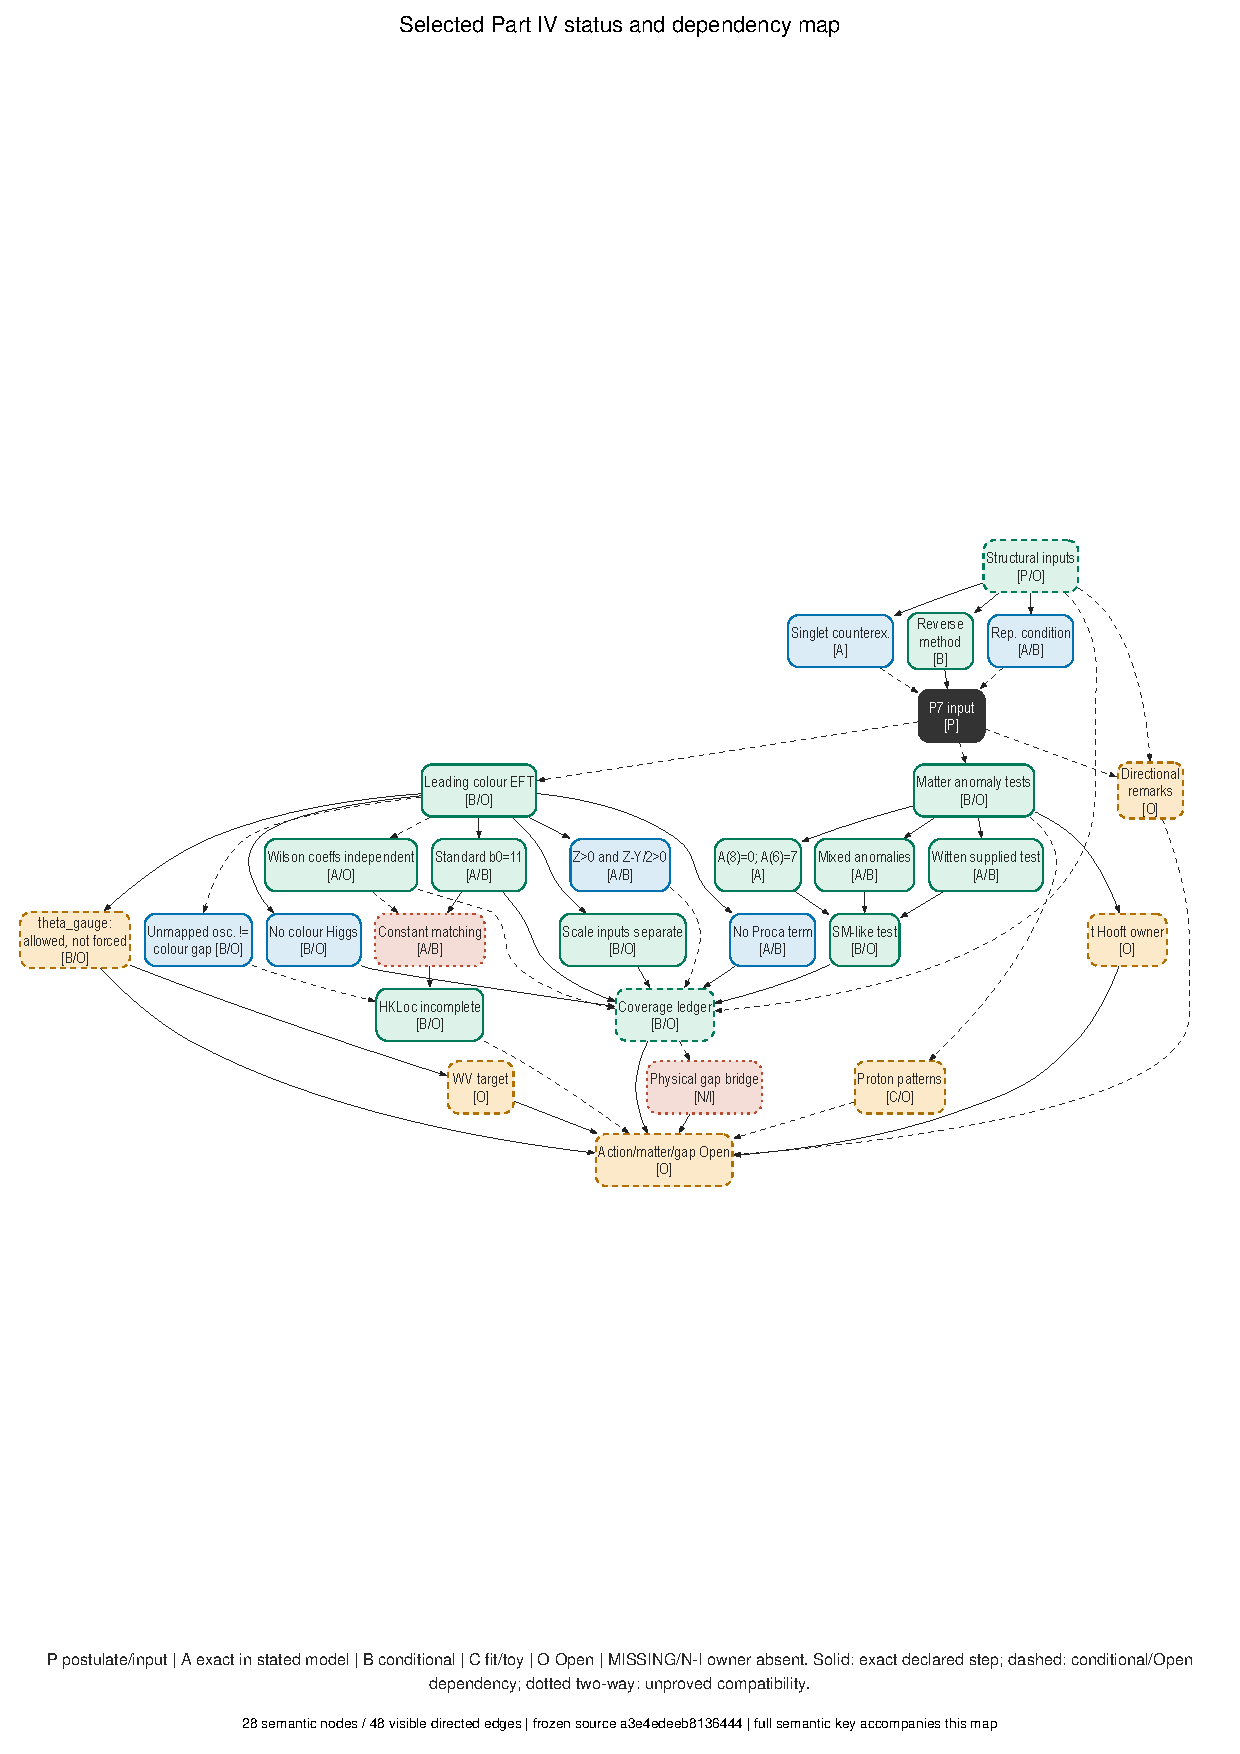
\includepdf[
  pages=1,
  pagecommand={\thispagestyle{empty}\phantomsection
    \refstepcounter{figure}
    \label{fig:partIV_derivation_logic}
    \label{app:r141_complete_part_iv_logic}
    \label{app:r129_visual_part_iv_logic}
    \label{appfig:r123_atlas_fig38}
    \label{appfig:r123_topology_fig38}
    \addcontentsline{lof}{figure}{\protect\numberline{\thefigure}Part~IV logic (P7 structural postulate and physical-colour constraints)}}
]{figures/r185/logic_maps/partIV_status_dependency.pdf}

\paragraph{Reading discipline.}
Solid arrows in Figure~\ref{fig:partIV_derivation_logic} denote declared
logical dependence or organisation and never upgrade node status.  Dashed
arrows expose conditional or Open connections to the forward programme.  The
same colour/luminance and direct-label policy as in the other maps preserves
the hierarchy under grayscale conversion.

\paragraph{Final statement for Part~IV.}
Part~IV preserves the adopted P7 $SU(3)$ structural postulate and a
separate physical-colour completion programme; it does not claim that the
postulate already supplies physical QCD.  The scoped stabiliser and direct-embedding
facts, the convention-fixed leading truncation, source-model RG algebra,
standard anomaly identities and local heat-kernel calculations survive.  The
reducible, emergent/nonlinear and defect-kernel routes also survive.  Physical
colour, coefficient matching, the multi-coefficient RG, $U(1)_B$, the
quark-mass phase, confinement, the global gap and the hadron spectrum remain
Open.

\clearpage
\part{Summary, Comparisons, and Outlook}
\label{part:summary}
%==============================================================

\section{Discussion}
\label{sec:discussion}

This section provides a consolidated discussion of the ECT framework:
its conceptual logic, status-and-dependency architecture, current
status-separated outputs,
comparison with neighbouring programmes, observational reach,
limitations, and future directions.

%--------------------------------------------------------------
\subsection{Conceptual interpretation and scope of the framework}
\label{subsec:conceptual_interp}

ECT investigates whether Lorentzian spacetime, quantum dynamics, and
gravitational interactions can all be obtained from one scalar medium in
four-dimensional Euclidean space.  P4 adopts the physically relevant
nonzero-gradient branch and supplies its chart; a stationary action, physical
formation/selection history and the cross-sector common owner remain Open.
This is an organising hypothesis investigated through statements of varying
status, as classified in Table~\ref{tab:ect-levels}; the conditional and Open
items do not provide evidence that a common physical owner exists.

This perspective inverts the conventional logic of quantum gravity.
Rather than attempting to quantise an existing spacetime geometry, ECT
starts from a fundamentally Euclidean arena where no distinction
between space and time exists, and recovers the Lorentzian structure
as a candidate effective property of the supplied ordered-gradient chart.  The
displayed scalar action gives a Lorentzian principal tensor; a physical
metric, clocks/rods and universal sector cone do not follow directly.
The thermodynamic arrow of time is addressed at the level of the
ordered-branch open-system description with clearly stated closure
assumptions~(Section~\ref{sec:second_law_basics}).
The same-medium hypothesis provides a common research framework for
$G_N$, the EFT action scale later matched to $\hbar$, and the scalar
speed map.  Their microscopic ownership and mutual relations are not
derived.

This framework should not be interpreted as claiming that time is
``unreal''.  It proposes that the distinction between temporal and spatial
directions may be a collective property of a future physical ordered state.  The present
result establishes only the conditional scalar principal-symbol
classification; a physical clock and universal metric remain to be derived.

The comparison with closely related Euclidean-to-Lorentzian
constructions~\cite{GirelliLiberatiSindoni2009,MukohyamaUzan2013}
is useful in a second respect as well. It shows that the
basic idea of obtaining Lorentzian characteristic operators from Euclidean
field theory is not unique to ECT, but it also makes clearer which parts of
ECT remain distinctive claims rather than generic consequences of that
shared idea: the Open programme for an action-owned spontaneous origin of the
preferred direction, the proposed gravitational completion, and the extension
to quantum and phenomenological sectors.

%--------------------------------------------------------------
\subsection{Status-and-dependency architecture: from the $\Phi$-medium to
Open observable completions}
\label{sec:derivation_architecture}

The status architecture of ECT can be summarised as a directed graph
from the foundational $\Phi$-medium to derived supplied-model results,
conditional reconstructions and Open completion targets
(Figure~\ref{fig:ect_derivation_map}).  The graph is status-separated; it is
not a claim that every major physical sector has emerged from P1--P6.

\paragraph{Step~1: the $\Phi$-medium and the foundational postulates.}
The starting point is a scalar condensate field~$\Phi$ living on a
four-dimensional Euclidean manifold $(M^4,\delta_{AB})$ with an
$O(4)$-invariant action $S_E[\Phi]$.
No external time coordinate is postulated.  P5 separately adopts a limited
operational relational-response principle based on invariant comparisons with
material and boundary probes; a complete relational quotient, physical
observable algebra, clock/rod construction and relational dynamics have not
been derived.

\paragraph{Step~2: adopted ordered-gradient branch and chart.}
Postulate P4 declares the physically relevant sector to have
$\langle\partial_A\Phi\rangle\neq0$ and supplies the representative
$n_A=\delta_{Aw}$.  The nonzero vector has $O(3)$ stabiliser inside $O(4)$.
The complete stationary state/action, stability, spontaneous formation and
dynamical selection from P1--P3, together with the descent of physical
macroscopic/quantum sectors, remain Open.

\paragraph{Step~3: conditional scalar Lorentzian classification.}
Perturbations around the ordered background experience the effective
ordered-branch kinetic tensor
$K^{AB}=\beta\,\delta^{AB}-\alpha\,n^A n^B$.
For a homogeneous ordered background $n^A=\delta^A_w$, the scalar
principal tensor is Lorentzian exactly when $\beta(\beta-\alpha)<0$.
On the separately declared healthy $\beta>0$ branch this is
$\alpha>\beta>0$, with
$K^{AB}=\mathrm{diag}(\beta,\beta,\beta,\beta-\alpha)$ and
$\hat c_*^2=\beta/(\alpha-\beta)$.
This yields a scalar common-length tensor proportional to
$\mathrm{diag}(-1,1,1,1)$ at $\hat c_*=1$; it is not yet a physical
light cone.

\paragraph{Step~4: macroscopic tensor branch (Part~II).}
The macroscopic sector develops as follows:
\begin{itemize}[noitemsep,topsep=2pt]
\item \emph{General relativity.} A separately supplied healthy
  Fierz--Pauli seed could self-couple to an Einstein--Hilbert closure
  under the standard assumptions.  At fixed $\alpha,\beta$ and tangent-director linear order about homogeneous
  $n=w$, the displayed map has no linear TT seed or static-density vertex,
  so the supplied tensor action is a completion target rather than a result
  of the scalar action; quadratic/nonlinear/composite routes remain Open.
  The scalar--tensor ansatz yields the corrected scalar metric and
  field equations.  A preferred-direction curvature operator resembling an
  Einstein--aether term is a proposed separate extension
  \cite{Jacobson2004}; it is not derived from the displayed scalar-only action
  and remains Open pending a covariant $n^A$ sector and projection audit.
\item \emph{Fundamental constants.}
  $G_N^{\rm nat}=(8\pi M_G^2)^{-1}$ is a conditional physical-tensor
  matching, while $c_{\rm char}=c_{\rm u}\hat c_*/\mathcal N_\Phi$ requires a
  clock map and $c_{\rm char}=c$ is the adopted scalar-clock calibration.
  None is derived from the condensate amplitude alone.  Independently,
  $\phi_0=\zeta_\phi\bar M_{\rm Pl}$ with $\zeta_\phi>0,\ \zeta_\phi=O(1)$ is the adopted
  Level-B scale ansatz; its microscopic explanation remains Open.
\item \emph{Scale inventory.}
  The energy/matching scales $\phi_0\sim\bar M_{\rm Pl}$ and
  $v_2\approx246$~GeV have distinct declared status.  The kpc quantity
  $L_{\rm gal}$ is a matching length used in Level-C HRC diagnostics, not a third
  field scale; its ECT origin is Open (Section~\ref{sec:three_scales}).
\item \emph{Cosmology.} The ordered branch supplies conditional
  background and perturbation constructions, not a completed numerical
  cosmology.  The fixed orientation determinant does not derive
  vacuum-offset decoupling.  A separately supplied trace-free completion is
  classically shift covariant through $V+C_I$, while a distinct ordinary
  two-slope completion gives a regular late-de-Sitter proof of class but is
  not additive-shift invariant.  Their descent from the $\Phi$ medium, the
  physical matter/photon metric, global state and likelihood remain Open.
  The primordial spectrum~$(n_s,A_s,r)$ is likewise an open target.
\item \emph{Galactic dynamics.} HRC-0 and HRC-3 are the active
  augmented-model response candidates; the slope~4 is conditional algebra
  after a separate static gravity bridge.  Existing SPARC/RAR/BTFR outputs are
  HRC-only algebraic diagnostics.  P1--P6 ownership, source/metric map, and the
  matched $a_{M0}=cH_0/(2\pi)$ coefficient remain Open as stated.
\item \emph{Strong-field sector.} A critical-shell ansatz supplies only
  the conditional Tolman crossover $\rho_*=\hbar c/(2\pi k_BT_*)$ and a
  candidate route to black-hole thermodynamics~(Level~C/Open).  No
  physical $T_*$ or universal shell thickness is derived.  Only the generic
  reduced-state identity is Level~A mathematics; global interacting
  unitarity, purification and the Page curve remain Open.
\item \emph{Preferred-direction programme.}  No coefficient or species law is
  derived, and the allowed vector operator does not generate a spin or
  body-force observable by itself.
  The homogeneous timelike vector term has no spin splitting, and the fixed
  spurion supplies no source-generated E\"otv\"os force.  The former numerical
  windows are withdrawn as outputs of this operator; external spin and WEP
  sensitivities constrain only a separately declared completion.
\end{itemize}

\paragraph{Step~5: quantum coherent branch (Part~III).}
In parallel, the coherent sector develops:
\begin{itemize}[noitemsep,topsep=2pt]
\item \emph{Action-scale candidates and operational unit.}  The supplied
  fixed-core and balanced loop closures define distinct coefficients; later
  conditional quantum formulae use an operational $S_0$ whose owner remains
  Open.  Winding gives integer labels.
  The phase-only model has no nonzero global minimum.  A supplied positive
  two-term 1D model has the exact conditional minimum
  $\mathcal I_{n,\min}=2\pi|n|\iota_{0,\rm bal}^{\rm eff}$, but its common 4D owner,
  carrier/ensemble stability, cross-sector universality and any matching to
  $\hbar$ remain Open~(Level~B/Open for ECT ownership).
\item \emph{Schr\"odinger equation.} A supplied linear coherent sector
  admits a conditional envelope reduction and the usual uncertainty theorem
  for supplied operators.  The physical operator/state map, CCR
  normalisation and universal $S_0$ are Open~(Level~B/Open).
\item \emph{Vacuum response.} Supplied scalar/QFT calculations compare
  a Dirichlet Casimir BVP, the standard Unruh/KMS target and
  time-dependent mode mixing.  A common physical ECT response bundle,
  state and coupling are Open; no condensate-sector Casimir ratio is
  predicted.
\item \emph{Decoherence and arrow of time.} The influence-functional
architecture yields environmental open-system closures and provides notation
for candidate record channels.  The Di\'osi--Penrose functional and its one
declared hard-sphere orientation point are external comparisons; an ECT
gravitational kernel remains Open.  An entropy-growth theorem and a Crooks relation remain Open ECT
constructions: the former requires a named channel/state/entropy functional
and contractivity conditions, while the latter requires forward/reverse
protocols and local detailed balance.
\item \emph{Born rule.} A complete applicable corrected OS-II package may
  reconstruct an inner product in a declared free model.  Independently,
  ordinary projector Gleason represents an admitted normalised, noncontextual,
  countably additive projector measure only for a complex Hilbert space with
  $\dim\mathcal H\ge3$; a qubit requires the Busch effect/POVM theorem under separately declared C2q hypotheses.  Neither result creates probabilities, selects an
  outcome, or derives the physical state/preparation, event, probability
  origin or update from P1--P6~(Level~A mathematics under the stated theorem
  hypotheses; ECT ownership Open).
\item \emph{Exchange topology and spinors.} The
  $\pi_1(\mathcal{M}_2)=\mathbb{Z}_2$ result from
  $d_{\rm spatial}=3$ is Level~A conditional topology for a supplied
  identical-point configuration space.  The physical particle map,
  spin-statistics hypotheses and Dirac matter action remain Open.
\item \emph{Entanglement.} Non-factorisable correlations follow only
  after a nonfactorising state and channel are supplied; a common ordered
  medium is insufficient~(conditional mathematics / Open ECT).
\item \emph{Area-law entropy programme.} A conditional finite-cell
  counting lemma is exact after a coarse-graining, finite local
  capacity, physical split and area-law state class are supplied.
  ECT ownership of those inputs, a physical black-hole bound and
  holographic reconstruction remain Open
  (Theorem~\ref{thm:area_bound}).
\item \emph{Charge quantisation.} Standard representation theory gives
  $q\in\mathbb{Z}\cdot e_0$ after a compact local $U(1)$ bundle, charge
  unit and matter representation are supplied (Level~A conditional
  mathematics).  ECT ownership of those premises, the unbroken photon and
  the observed Standard-Model charge spectrum remains Open.
\item \emph{Post-transition cosmological branch classification.}
  ECT does not yet derive the full nonequilibrium transition or
  the selection of the expanding branch from first principles,
  and a named supplied completion exhibits a regular expanding,
  early-decelerating, late-accelerating history.  P1--P6 do not select
  that completion or history; thermal, recombination, perturbation and
  CMB closures remain Open~(\S\ref{sec:post_transition}).
\item \emph{PES-R operational programme.} PES-R is a bounded
  Level-B organising taxonomy for dynamical admissibility, finite-time
  retention, and pairwise records.  Visibility and qubit/CHSH numbers are
  declared source-model or toy proxies; they do not derive Born weights,
  measurement outcomes, spectra, or a universal quantum--classical boundary.
  ECT-specific kernels and record operators remain Open.
\end{itemize}

\paragraph{Step~6: gauge and matter sectors.}
BR1 supplies a compact global phase.  A local $U(1)$ bundle, unbroken
photon, charge map and matter representations do not follow from that fact;
the non-Abelian $SU(2)$ completion, $W^\pm/Z$ identification and radial-mode
Higgs map are likewise conditional model-building routes (Level~B/Open).
The colour group $SU(3)$ and the fermion-generation structure remain Open.
The adopted P7 $SU(3)$-structured bundle is analysed in
\S\ref{sec:colour_completion}; its identification with physical colour and any
baryon-number selection rule remain Open.

\paragraph{Particle spectrum.}
The condensate architecture organises the particle sector into
different status layers.
At the structural or partially established level this includes:
a physical graviton only as an Open tensor-completion target (the fixed $\delta n_A$ map has no linear TT/static-density seed only at fixed $\alpha,\beta$ and tangent-director order about homogeneous $n=w$; quadratic/nonlinear alternatives remain parametric/Open);
the photon, $W^\pm/Z$, Higgs and fermions only as targets of supplied
gauge/matter completions; their physical bundle, representation, mass and
observable maps remain Open.
The strict integrability-reduced orientation map instead retains one
longitudinal scalar coordinate $\chi$.  A one-mode physical EFT is conditional;
its existence, mass, abundance and possible cosmological or dark-sector role
remain Open.  For the primary
$\pi_3(S^3)$ sector, topology supplies integer labels only and the
two-derivative energy $E_2(R)\propto R$ collapses.  Any finite particle and
mass spectrum requires a separately derived stabilising action; a possible
secondary-sector owner remains Open.

\paragraph{Step~7: results, benchmarks, tests, and Open gates.}
The map separates strict results from matched benchmarks and explicitly
declared closures.  In particular, $a_M$ and the gravity bridge remain matched/Open;
the deep-HRC slope~4 is Level~A only inside the supplied functional,
conditional after that bridge, and its data comparison is Level~C.  The
no-halo statement is only a property of the stated diagnostic fit,
and environment/orientation signals remain Open programmes.  None predicts
the absence of particle dark matter or of a laboratory signal.
These are summarised in
Figure~\ref{fig:ect_derivation_map} and Tables~\ref{tab:ect_structure}
and~\ref{tab:ect-levels}.

\paragraph{Complete programme map.}
Figure~\ref{fig:ect_derivation_map} is a selected ECT programme
graph.  It places postulate/structural inputs, conditional closures, Level-C
benchmarks and Open owner maps on one topology-preserving A4 reader map.
The map includes the corrected coherent-branch, T1, OS-II, admitted-measure
and PES-R routes.  It does not contain a direct Schr\"odinger-to-Born edge or
an automatic T1-to-$\hbar$ edge.

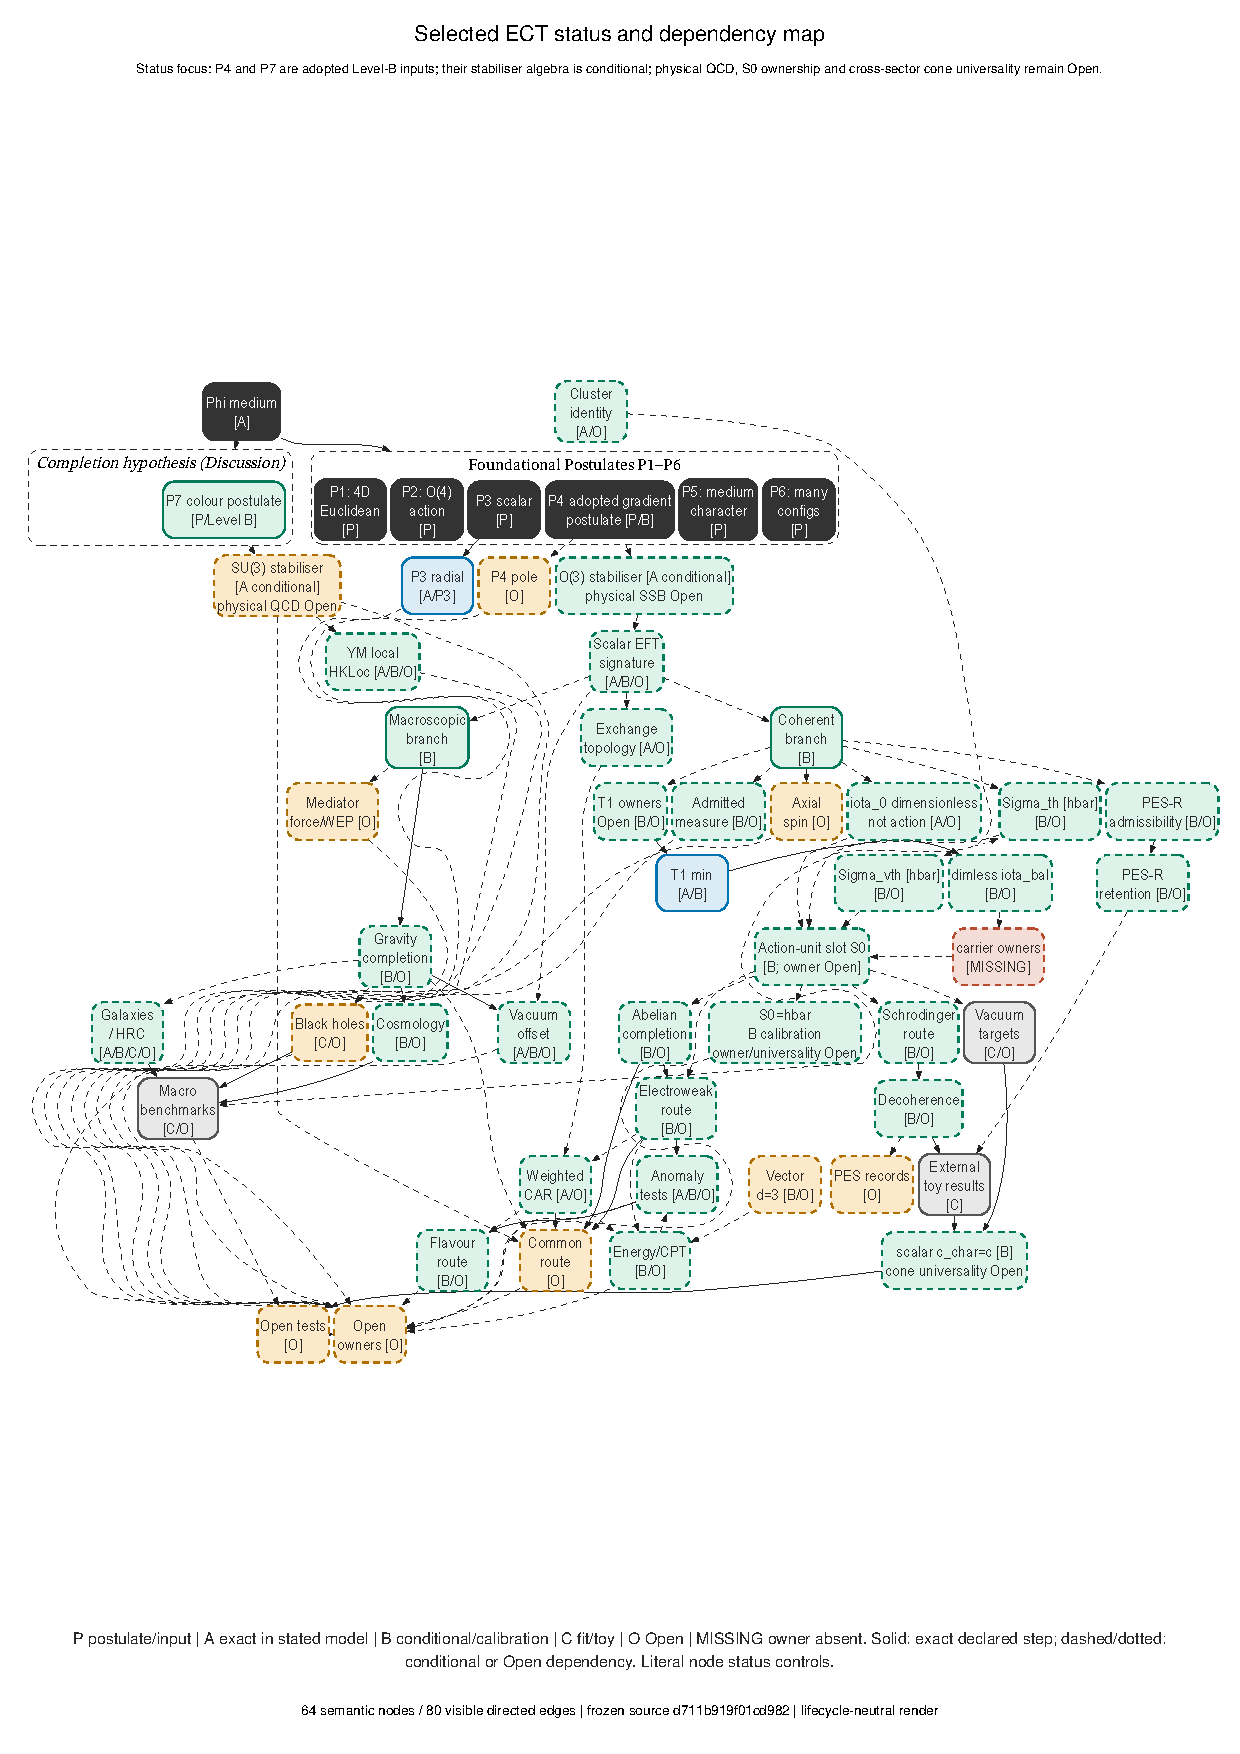
\includepdf[
  pages=1,
  pagecommand={\thispagestyle{empty}\phantomsection
    \refstepcounter{figure}
    \label{fig:ect_derivation_map}
    \label{app:r141_complete_full_derivation_map}
    \label{app:r129_visual_full_derivation_map}
    \label{appfig:r123_atlas_fig39}
    \label{appfig:r123_topology_fig39}
    \addcontentsline{lof}{figure}{\protect\numberline{\thefigure}Selected ECT status and dependency map}}
]{figures/r185/logic_maps/whole_status_dependency.pdf}

\paragraph{Reading discipline.}
Solid arrows in Figure~\ref{fig:ect_derivation_map} organise declared
dependencies; dashed arrows identify assumptions, matching steps or
incomplete routes.  Galactic nodes marked ``matched'' or ``conditional'' are
not particle-ontology conclusions.  Likewise, the generic fifth-force node
refers only to a separately supplied dynamical mediator/profile, source and
body charges, propagator, range and screening; the fixed homogeneous vector
spurion is not such a force.  The coherent-quantum gate still requires the
applicable OS-II/Hilbert structure and an independently admitted measure;
physical preparation, probability, outcome and update remain Open.  The
A4 reader map, its frozen source, deterministic exact key and the machine topology are jointly
authoritative; the former fragmented reader pages and printed edge ledgers
are not part of the current reader layer.

%--------------------------------------------------------------
\subsection{What ECT already establishes: emergence chains and
current status}
\label{subsec:emergence_chains}

The programme claim of ECT is that several major physical frameworks
can be organised within one ordered-condensate architecture as exact
mathematical sectors under stated assumptions, conditional limits, or Open
completion routes.  These categories are kept distinct throughout; no
single statement here claims their completed physical recovery.

\paragraph{General relativity.}
The supplied ordered scalar EFT conditionally yields a Lorentzian scalar
principal/propagation sector.  At fixed $\alpha,\beta$ and to linear order in
a tangent director perturbation, the fixed director image generates neither
a linear TT seed nor a linear static-density vertex.  This scoped component
theorem does not exclude nonlinear, composite, additional-field, or
dynamical-parameter vertices; the general physical tensor/source/metric map
remains Open.  A Fierz--Pauli structure and Einstein closure are supplied
completion targets.  In a separately declared pure-metric completion the
Einstein--Hilbert form is the unique two-derivative closure in four dimensions
under its standard assumptions.
\emph{Status: Level~A mathematics inside the supplied scalar and pure-metric
assumptions; the negative fixed-map result is Level~A only in the scoped
linear fixed-parameter limit; physical metric/tensor/source completion Open.}


\paragraph{Quantum coherent dynamics.}
The corrected quantum programme has a strict separation of owners.  Sector
operators, domains, representations, and boundary conditions supply spectra
and coherent dynamics; a complete applicable corrected OS-II package supplies
the Hilbert-space reconstruction only in the declared subsectors where every
hypothesis has been checked, with reflection positivity only one member of
that package.  Specified influence functionals supply reduced-state response
and pairwise records.  Independently, ordinary projector Gleason represents a
supplied probability measure only after its dimension, projector-algebra,
normalisation, noncontextuality and countable-additivity hypotheses are
admitted.  PES-R then classifies already admissible modes by finite-time
retention and declared record comparisons.  It derives neither $S_0=\hbar$,
Born weights, unique outcomes, universal compact-phase quantisation, nor a
Crooks relation.  The interacting Hilbert-space completion, ECT record
operators and state, detector update rule, physical tensor quantisation, and
forward/reverse path measures remain Open.  This is a smaller but logically
stronger programme than the former one-functional selection picture.


\paragraph{Decoherence and the macroscopic arrow of time.}
ECT contains a causal response backbone and can host specified reduced-state
channels.  Environmental estimates reproduce declared source models, while
the gravitational values are external Di\'osi--Penrose benchmarks.  A Crooks
or entropy-production theorem requires explicit reduced dynamics,
forward/reverse protocols, local detailed balance, and initial ensembles;
these ECT-specific ingredients remain Open.

\paragraph{PES-R and quantum reconstruction.}
PES-R separates sector dynamics, finite-time retention, and pairwise record
robustness.  Spectra, least action, Born weights, and measurement outcomes
remain owned by their separate derivations/Open programmes.  Thus PES-R is a
Level-B/Open organising taxonomy, not a universal selection mechanism.

\paragraph{Galactic weak-field phenomenology.}
HRC-0/HRC-3 are the active augmented-model response candidates.  The
BTFR/RAR and rotation-curve benchmarks have been recomputed as HRC-only
Level-C algebraic diagnostics, not full field predictions.  The live-action gravity map,
environment law and particle content remain Open.
\emph{Status: augmented-model A/B; frozen fits C; live ECT Open.}

\paragraph{Gauge and matter sectors.}
ECT provides a condensate framework in which conditional gauge and
matter completions can be formulated.  Physical local bundles, unbroken
gauge fields, representations, anomaly-complete chiral matter, and the
coupling hierarchy are not derived from P1--P6.
\emph{Status: conditional structural programme with these physical owners
Open.}

\paragraph{Interpretive conclusion.}
The correct claim is therefore not that every established theory has
already been rederived as a completed Level~A theorem.
Rather, ECT organises general relativity, coherent quantum dynamics,
the Hilbert-space bridge, decoherence, vacuum-response effects,
entanglement, black-hole thermodynamics, the dark-sector ontology,
and the analogue-laboratory programme inside one common
ordered-medium picture while making explicit which parts are
structural, which are structurally singled out but not fully closed,
and which remain open.


%--------------------------------------------------------------
\subsection{Architectural comparison with neighbouring programmes}
\label{sec:comparison}

The purpose of this subsection is not to argue that ECT is ``better''
than all neighbouring frameworks.
It is to locate ECT within the broader landscape of approaches to
emergent spacetime and quantum gravity, highlighting where its
architectural choices overlap with, differ from, and remain weaker or
stronger than those of its neighbours.

\paragraph{Scope and methodology.}
The comparison is organised along eight structural axes:
origin of time/Lorentzian structure,
origin of gauge structure,
origin/status of quantum axioms,
gravity closure,
dark-sector treatment,
singularity logic,
information/decoherence architecture,
and falsifier structure.
Table~\ref{tab:comparison_main} summarises the comparison; an expanded
version with additional axes is given in
Appendix~\ref{app:comparison_expanded}.

\paragraph{Comparison by test structure.}
A completed common-origin ECT model could have correlated cross-sector tests
if one owner chain fixed several observables.  No such global chain is
derived here.  At present, failure of one supplied cone, action-scale or
ultraviolet completion rejects that completion, not P1--P6 as a whole.
Standard particle, gravitational and cosmological theories likewise have
tests at the level of their stated models and parameter sectors; no
literature-wide superiority or uniqueness claim is made.

\paragraph{Comparison by number of independent primitives.}
Reducing the number of independent foundational primitives is an ECT design
aim, not an established comparison metric.  General relativity supplies a
metric/diffeomorphism framework and the Standard Model supplies quantum gauge
and matter sectors; neither theory by itself specifies a cosmological dark
sector.  Standard $\Lambda$CDM applications add cold dark matter and
$\Lambda$ as separately parameterised components.  ECT asks whether some of
these structures can descend from one ordered medium, but it has not derived
the physical metric/tensor sector, quantum axioms, Standard-Model gauge and
matter content, or a dark-sector completion.  A quantitative like-for-like
parameter census remains Open~(Section~\ref{sec:parameter_compression}).

{
\small
\renewcommand{\arraystretch}{1.2}
\begin{longtable}{@{}L{2.3cm}L{2.3cm}L{2.3cm}L{2.3cm}L{2.3cm}L{2.3cm}@{}}
\caption{Architectural comparison of ECT with neighbouring programmes.
Entries are necessarily compressed; for expanded discussion see
Appendix~\ref{app:comparison_expanded}.}
\label{tab:comparison_main}\\
\toprule
Axis & GR + SM & Einstein-aether & Ho\v{r}ava--Lifshitz
  & Volovik analogue & ECT \\
\midrule
\endfirsthead
\toprule
Axis & GR + SM & Einstein-aether & Ho\v{r}ava--Lifshitz
  & Volovik analogue & ECT \\
\midrule
\endhead
\midrule
\endfoot
\bottomrule
\endlastfoot
Time / Lorentz
  & Fundamental
  & Fundamental; preferred frame added
  & Fundamental but anisotropic
  & Emergent from condensate
  & Conditional scalar Lorentzian principal tensor after supplied P4 and
    $\beta(\beta-\alpha)<0$ (or $\alpha>\beta>0$ on the retained
    $\beta>0$ component); physical time, clock, and universal sector cones
    Open \\
Gauge structure
  & Postulated
  & Postulated
  & Postulated
  & Analogy only
  & Ordered-branch structural route to $U(1)$ and $SU(2)$;
    physical SM identification incomplete; $SU(3)$ open \\
Quantum axioms
  & Primitive
  & Primitive
  & Primitive
  & Primitive
  & Structural route via coherent branch; completion open \\
Gravity closure
  & Einstein eqs.\ exact
  & Einstein + aether
  & Modified dispersion
  & Acoustic metric only
  & Scalar characteristic geometry; physical metric/tensor/source Open \\\
Dark sector
  & Extra particles + $\Lambda$
  & Extra particles + $\Lambda$
  & Extra particles + $\Lambda$
  & Not addressed
  & No-halo Level-C HRC data diagnostic; ECT particle content and matching Open \\
Singularities
  & Physical or censored
  & Physical or censored
  & Possibly resolved by UV
  & Not addressed
  & Candidate branch-boundary or condensate-breakdown interpretation;
    microscopic completion and replacement dynamics Open \\
BH information
  & Paradox open
  & Paradox open
  & Modified; details model-dependent
  & Not addressed
  & Reduced-state information reading; fundamental loss not required
    within the present programme, but completed evaporation closure
    remains open \\
Falsifier style
  & Sectorwise
  & Extra-mode / LIV
  & LIV / dispersion
  & Not systematic
  & Named-completion sectorwise; cross-sector only after a common owner \\
\end{longtable}
}

\paragraph{What ECT still does not derive.}
The comparison above should not be read as implying that ECT has already
completed all structural derivations that are postulated in the standard
framework.
The main unresolved fronts are summarised more systematically in
Section~\ref{sec:limitations}.

\paragraph{Interpretive note.}
The comparison above is architectural, not polemical.
Each listed programme has independent strengths that ECT does not
replicate.
The point is not that ECT solves all problems, but that it pursues a
distinctive architectural strategy---single ordered medium, emergent
spacetime and quantum structure, cross-sector falsifiers---that is
worth comparing on its own terms.

The remarks below complement the architectural comparison of this
section and the extended discussion in
Appendix~\ref{app:comparison_expanded} by relating ECT to several
further emergent-gravity programmes that emphasise different
aspects of the same underlying question.

\paragraph{Sakharov's induced gravity.}
Sakharov's induced-gravity programme~\cite{Sakharov1968} treats the
Einstein--Hilbert action as effectively induced by quantum fluctuations
of matter fields propagating on a pre-existing Lorentzian metric.
ECT shares the structural conclusion that the gravitational action
need not be fundamental, but addresses a complementary level in the
theoretical structure: in a supplied branch ECT constructs a scalar
characteristic-tensor candidate from the condensate order parameter $n_A$
on a Euclidean background; whether it is the physical metric remains Open.
Sakharov's mechanism addresses why $\int\sqrt{-g}R$ appears given a
metric, whereas ECT poses a programme for deriving a physical metric from
the medium.

\paragraph{Verlinde's entropic gravity.}
Verlinde's programme~\cite{Verlinde2011} interprets gravity as a
thermodynamic, entropic effect arising from information associated
with holographic screens. ECT shares the broad motivation that
gravity need not be a fundamental interaction, but addresses a
different aspect of the emergence problem: it provides a concrete
medium-action candidate route through variation of a microscopic
condensate action rather than an information-theoretic re-derivation; the
physical metric/source/gravity map remains Open.  An entropic reading, if
valid, would be consistent with a thermodynamic shadow of the same
candidate condensate dynamics.

\paragraph{Kleinert's world-crystal picture.}
Kleinert~\cite{Kleinert2008} models curvature in terms of defect
densities (disclinations and dislocations) in an effective elastic
medium, with the gravitational field arising from elasticity theory
on a world-crystal. ECT shares the philosophical position that
gravity admits an underlying medium, but the medium in ECT is a
continuous condensate field $\Phi$ on a Euclidean manifold rather
than a crystalline lattice. ECT therefore does not invoke an
explicit discretisation; the role of geometric response is encoded
in the gradients of the orientation field $\nabla_\mu n_\nu$,
with no defect-density interpretation required at the level of the
ordered-branch EFT.

% ------------------------------------------------------------------
\subsection{Comparison with alternative quantum interpretations}
\label{sec:comparison_interpretations}

\paragraph{Cramer's transactional interpretation (TI).}
Cramer~(1986)~\cite{Cramer1986} models every quantum interaction as
an exchange of ``offer'' (retarded) and ``confirmation'' (advanced)
waves between emitter and absorber.
ECT shares with TI the structural idea that the relevant coherent-sector
description is not exhausted by a purely one-sided Lorentzian-causal
picture.
In TI this appears as the advanced--retarded offer/confirmation
language.
In ECT it appears through the two-sided boundary sensitivity of the
Euclidean coherent branch.
The similarity is therefore real but not an identity:
TI is an interpretation of the standard quantum formalism, whereas ECT
locates the two-sided structure in a specific Euclidean condensate
ontology.
The present comparison is conceptual and structural; it is not the
claim that TI is fully derived as a special case of ECT.
ECT therefore does not adopt the literal offer/confirmation-wave
ontology of TI.
The overlap lies only in the structural rejection of a primitively
one-sided temporal description.

\paragraph{Page--Wootters mechanism.}
Page \& Wootters~(1983)~\cite{PageWootters1983} proposed that effective
time can arise from entanglement between a ``clock'' subsystem and the
rest of the universe within a globally stationary state.
ECT shares the motivation of avoiding a fundamental external clock.
Page--Wootters reconstructs relational time inside a supplied quantum state.
P4, by contrast, adopts the physically relevant ordered-gradient
sector and its preferred Euclidean direction.  A temporal parametrisation of
a supplied hyperbolic scalar operator is conditional, while a physical
clock/lapse, quantum state and universal metric remain Open.  The
comparison therefore identifies two possible reconstruction programmes; ECT
does not yet provide a deeper physical derivation of a time-bearing branch.


% ==============================================================
\subsection{ECT as a foundational framework for quantum mechanics}
\label{sec:ect_vs_qm}
% ==============================================================

The detailed structural comparison between ECT and the standard
quantum formalism---covering the hierarchy of effective equations,
the boundary-value versus Cauchy problem, the ontological distinction
between $\Phi$ and $\psi$, the origin of the statistical description,
the concept mapping onto the standard quantum primitives, and the
illustrative examples of interference, tunnelling, measurement,
entanglement, and identical particles---is developed as the capstone
of Part~III in Section~\ref{sec:qm_capstone}.  The role of the
present subsection is not to duplicate that material, but to close
two pan-structural threads of the comparison that naturally belong
to the summary chapter: the common origin of the coherent and
geometric branches of ECT, and a compact overall summary of the
ECT-versus-QM relation that also serves as a bridge to the broader
architectural comparison with neighbouring programmes.

% ------------------------------------------------------------------
\subsubsection*{Unified origin of the coherent and geometric branches}

ECT proposes that gravity and quantum coherence may be two sectors of
one ordered condensate completion.  The present scalar action does not
yet derive either a physical TT gravity sector or the full interacting
quantum theory, so this is an architectural hypothesis rather than a
closed result.

Candidate scalar kinematics in the two programmes may reuse the supplied
principal-tensor template $K^{AB}$, but no common physical action has been
derived.  In the strict P4 scalar map, $\chi$ is the longitudinal coordinate
defined by $\delta Q_A=\partial_A\chi$ and has the same field units as $\Phi$;
in BR1, $\theta$ is a dimensionless compact phase with its own independently
supplied stiffness $K_\theta^{\rm eff}$.  Their variables, coefficients,
action magnitudes and states are not identified.  The long-wavelength
geometric and shorter-wavelength coherent readings therefore remain candidate
programmes of one ordered-medium architecture.  ECT asks whether a completed
ordered-condensate action can generate both; the displayed ordered functional
does not yet establish that descent, and the common microscopic owner and
back-reaction vertex remain Open.

The scalar mode decomposition is exact inside the supplied ansatz, but
its identification with physical gravity and quantum mechanics is not.
In this sense ECT proposes, rather than has yet demonstrated, a common
substrate.

The supplied scalar Einstein sector contains the exact divided coefficients
$G_{\rm div}(X)$ and $\Lambda_{\rm div}(X)$, and admits separately proposed
tensor structures involving the ordered direction $n_\mu$.  Neither divided
coefficient is by itself a physical response map.
Conversely, in a completion that identifies the relevant amplitude variables
and supplies a common action-owned vertex, coherent fluctuations could affect
the effective amplitude sector and thereby back-react on the geometric side.
No common action-owned backreaction vertex between the coherent and physical
geometric/tensor sectors has yet been derived.  Their possible common medium
is an architectural hypothesis; a completed quantitative backreaction action,
state and observable map remain Open.

Closing this common-origin map is one of the most important Open
programmes of ECT.

% ------------------------------------------------------------------
\subsubsection*{Summary of the comparison}

Standard quantum mechanics is an effective statistical theory of
subsystems, formulated in terms of a probabilistic amplitude $\psi$
and a forward-time Cauchy problem.
ECT proposes a deeper level in which the fundamental object is the
physical condensate field $\Phi(X)$, governed by a global
four-dimensional boundary-value problem.
Selected quantum mathematical structures can be reproduced conditionally
after a coherent sector, state, continuation, operator normalisation and
reduction map are supplied.  Quantum mechanics as a complete physical theory
is not yet recovered; the owner-by-owner status is given in
Section~\ref{sec:qm_capstone}.

ECT therefore sets a programme to reproduce and ultimately explain the
effective quantum formalism (Fig.~\ref{fig:ect_vs_qm}).  Probability,
outcomes/collapse, interacting superposition, universal $\hbar$, physical
gravity and their common microscopic owner are explicit Open targets, not
current explanations.

\begin{figure}[H]
\centering
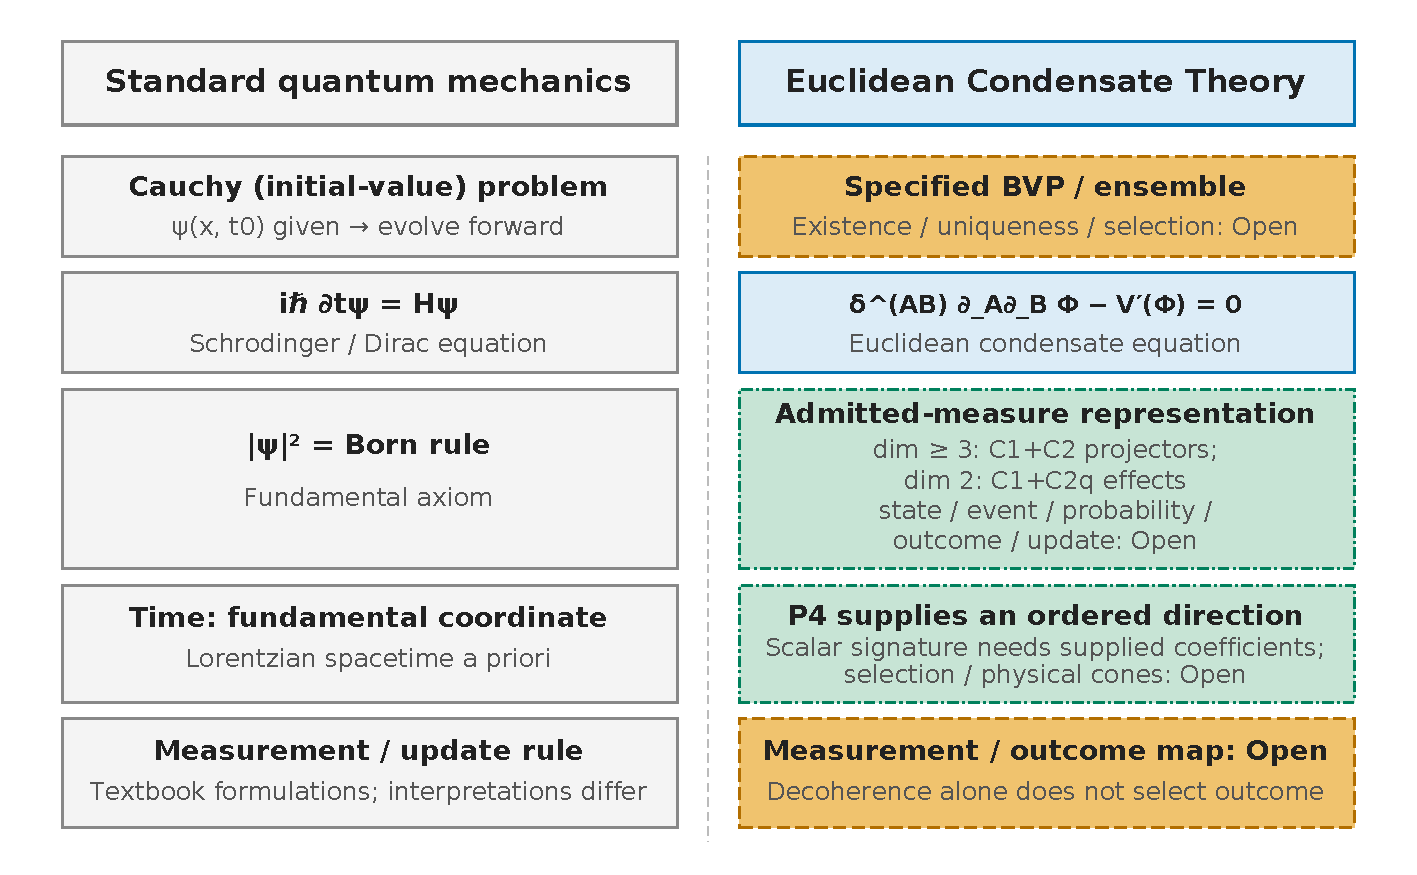
\includegraphics[width=\textwidth]{figures/r153/fig_ect_vs_qm_status_palette_r153.pdf}
\caption{Status-sensitive comparison of textbook quantum mechanics and the
current ECT programme.  The standard-QM column is an external comparison.
Within ECT, the supplied Euclidean scalar equation is model-internal, the
ordered-direction statement is conditional, and the BVP selection, Born
weights/reconstruction and outcome map remain Open.  Literal status wording
is authoritative.  Neutral, blue, green and amber luminance-ordered fills
provide redundant external, model-internal, conditional and Open cues;
solid, dash-dotted and dashed borders preserve the same distinctions without
colour.}
\label{fig:ect_vs_qm}
\end{figure}


In this sense, ECT does not replace standard quantum mechanics as a
laboratory calculation tool; it proposes a deeper level from which
standard quantum mechanics emerges as an effective, statistically
formulated subsystem theory.





%--------------------------------------------------------------
\subsection{Phenomenological reach and observational diagnostics}
\label{sec:obs_diagnostics}

This subsection collects the main observational implications and
detection strategies of ECT in one place, covering both dark-sector
diagnostics and the most informative empirical tests.

\paragraph{Tests of the HRC no-halo algebraic diagnostic.}

The Level-C HRC data diagnostic is tested with held-out kinematics and
prespecified transition/environment regressions.  Lensing becomes a test
only after a covariant two-potential metric completion; the current cluster
proxy does not supply it.  The diagnostic
contains no particle-halo term, but this does not identify a condensate
mechanism, exclude a particle flux, or predict a laboratory null result.
The exact local-response theorem preserves input ordering and the
set-valued argmax of the supplied total projected baryon proxy, even when the
argmax sets are empty.  Whenever maxima are attained, it forbids local
displacement of a total-response maximizer relative to that input; it does
not forbid an inherited gas/BCG offset or residual-map extrema and is not
morphology evidence or a derived condensate redistribution.

Possible particle, soft, or topological excitations have Open spectra,
couplings, abundance, and observables.  Their absence from the minimal fit is
not evidence that they are ultra-light, feebly interacting, or unnecessary.

\paragraph{Tests of the late-time scalar-background closure.}

The background ansatz may be compared with BAO, supernova, weak-lensing,
redshift-space-distortion, and growth data through its declared $H(z)$ and
$w(z)$.  Such comparisons test that closure.  They do not establish that the
microscopic condensate is the dark-energy source or that an independent
component is absent.  If the closure parameters are effectively frozen, its
background becomes observationally close to $\Lambda$CDM and discrimination
requires prespecified perturbation/growth observables.

\paragraph{Cluster-merger status.}
Equation~\eqref{eq:cluster_local_argmax_nogo} is the exact analytic result:
a strictly increasing local response preserves all ordering and the
set-valued argmax of the supplied total projected baryon proxy.  Whenever
maxima are attained, it cannot dynamically displace a total-response
maximizer, but it may inherit an input gas/BCG separation and
does not constrain the residual map.  Separately, identifying
$\tau_{\rm pole}=\tau_{a_M}^{\rm match}$ with one constant real Debye pole
and ballistic transport is excluded by the three-order scale mismatch; this
does not exclude general retarded kernels.  A physical explanation requires
the causal state evolution, matter and photon metrics, two lensing potentials,
hydrodynamic/collisionless initial data and a mock-observation likelihood
listed in Appendix~\ref{app:ect_cosmology_observable_protocols}.

\paragraph{The Great Attractor and large-scale peculiar flows.}
An ECT prediction of the Great Attractor or any large-scale peculiar-flow
field requires a calibrated inhomogeneous cosmological solution, a derived
matter-source and photon-metric map, survey selection and a velocity
likelihood.  These owners have not yet been supplied (OP21).  In the
restricted near-GR same-metric/quasistatic closure, the linear $aHfD$ carrier
differs from its matched control by only $0.00282$--$0.00293\%$ over
$0\le z\le2$ [Eq.~\eqref{eq:ect_restricted_peculiar_velocity}].  This gives
no material large-flow enhancement and is not a survey bulk-flow prediction.

\paragraph{Tests of the HRC galactic programme.}
Void dwarfs, diffuse groups, and outer disks are useful prespecified
low-acceleration stress-test populations for HRC-0/HRC-3.  The active
registry defines the current algebraic diagnostics.  Their placement on a
canonical scalar-screening diagram has not been derived.  Environment-tagged
samples may test prespecified $\Xi$ models and transition-shape correlations;
neither an external-field effect nor a signed trend is presently an ECT
prediction.

\paragraph{SPARC rotation-curve transition.}
The 165-galaxy statistics in Table~\ref{tab:sparc_summary_main}, now report HRC-only held-out diagnostics with signed gas.  They are
Level~C and do not replace the required finite-disk, nuisance-consistent
publication likelihood; the representative Milky-Way sensitivity is reported in the same HRC
registry but is not a modern joint posterior.  The scale $a_{M0}=cH_0/(2\pi)$ remains matching, and no
environment/history or external-field law is derived.

\paragraph{Lorentz-invariance violation gate.}
A viable ECT completion must make the physical gravitational,
electromagnetic and any additional massless modes pass stringent
relative-cone tests.  The present scalar action does not predict their
equality.
The joint GW170817/GRB~170817A analysis constrains
$-3\times10^{-15}\le(c_{\rm GW}-c_\gamma)/c_\gamma\le+7\times10^{-16}$
under its source-association and emission-time assumptions
\cite{LIGO_Fermi_GW170817_GRB2017}; this is an external kill gate for the
missing tensor/photon completion, not a check satisfied by construction.

\paragraph{Late-time-source acceptance test.}
A physical ECT late-time result must be produced by the same varied action,
state and matter/photon metric that determine $H(a)$, distances and the
gauge-reduced perturbations.  BAO, supernova, chronometer, growth and lensing
data then test that completion jointly.  At the present closure level no
numerical equation-of-state trajectory or likelihood is identified.

\paragraph{Summary of observational strategy.}
Held-out kinematic and lensing data can test the conditional HRC galactic diagnostic and separate cluster benchmark, while prespecified regressions can test named Open
environment extensions.  Candidate soft or topological sectors acquire
observable signatures only after their action, spectrum, abundance,
couplings, and source projection are derived.  These are closure-specific
tests and Open programmes, not current universal ECT predictions.

\paragraph{Systematic role of the orientation proxy.}
The manuscript inventories how a candidate $\mathcal X^{\rm cand}_{\mu\nu}[n]$ extension
would enter background, galactic, growth, and cluster calculations
(Table~\ref{tab:nlee_footprint}).  This is a sensitivity study, not a
derivation from the scalar action.  Sub-horizon growth and cluster lensing
appear most responsive in the proxy, but the orientation action, physical
projection, sign, and coefficient must be established before any of the
quoted corrections becomes an ECT prediction.

%--------------------------------------------------------------
%--------------------------------------------------------------
\subsection{Parameter compression and comparison}
\label{sec:parameter_compression}
%--------------------------------------------------------------

ECT motivates a possible parameter-compression programme, but no complete
owner/parameter census yet exists.
At the benchmark level used in the present synthesis, the condensate-side
description contains two kinds of ingredients:
(i) a kinematic branch choice, encoded in the kinetic coefficients
$\alpha,\beta$, and
(ii) non-kinematic condensate data, encoded in the gradient scale $u_0$,
the amplitude scale $\phi_0$, and the quartic coupling $\lambda$.
Adopting the Level-B unit-slope coefficient benchmark $\hat c_*=1$
gives $\alpha=2\beta$; a common field rescaling cannot select this ratio.
The numerical convention $\alpha=2,\beta=1$ fixes the remaining overall EFT
normalisation but does not derive the photon or tensor speed map.  The
separate physical equality $c_{\rm char}=c$ is the adopted clock calibration.
The triplet $(u_0,\phi_0,\lambda)$ is only the displayed condensate-side
subset.  Additional branch coefficients, actions, states, response
functionals, matching scales, operators and observable maps enter the
macroscopic, gauge/matter and quantum completions.

These inputs do not by themselves derive the advertised low-energy sectors.
The dimensionless scalar slope, characteristic cone and Klein--Gordon form
are Level~A inside the supplied scalar EFT.  The physical clock/photon map,
$S_0=\hbar$ is the explicit Level~B calibration and the physical owner and
$G_N$ completion remain Open; the Schr\"odinger envelope is a
conditional coherent-sector reduction; a physical tensor completion and
Einstein dynamics are Open.  Horizon/flatness/relic statements and late-time
backgrounds belong to named supplied completions, decoherence is conditional
open-system algebra with ECT kernels/state Open, and black-hole entropy and
information remain Open programmes.
The galactic rotation-curve and BTFR results reported in this version have
a different, explicitly layered status: they are conditional HRC
algebraic diagnostics after a supplied identity gravity bridge.  The HRC
response algebra is Level~A only inside the augmented response model;
ownership of its source/force map by the live condensate action remains
Open, and comparison with observations is Level~C.
At the more exploratory level, ECT also provides structural routes
toward $\alpha_{\rm fs}$, generation number, and Yukawa hierarchy.

A numerical comparison with the Standard Model plus cosmology would not yet
be like-for-like: ECT has not derived many parameters that those theories fit,
and its own completion data have not been counted.  Quantitative compression
is therefore an Open falsifiable target: it may be claimed only after one
owner-complete action/state/observable system reproduces the same data with a
fully disclosed independent-parameter count.

%--------------------------------------------------------------
\subsection{Completion data and residual bifurcation points}
\label{sec:completion_data}
%--------------------------------------------------------------

The remaining non-closed sectors of ECT fall into three
conceptually distinct classes, following the classification of
incompleteness introduced in this section.

\paragraph{Type~1: Initial-condition-sensitive sectors.}
The arrow of time, thermodynamic irreversibility, and the second law
depend not on a different ``branch of laws'' but on the realized
initial state.
This is not a special weakness of ECT: every fundamental theory
(GR, QFT, string theory) requires initial conditions for the
temporal asymmetry.
ECT offers a candidate route: a future physical $O(4)\to O(3)$ transition
could generate a non-equilibrium, coherent, low-entropy starting state.
The present theory does not derive that transition or show that this outcome
is generic; accordingly,
ECT does not yet derive a strict second law from first principles.

\paragraph{Type~2: Open microphysics.}
This class includes: the CP-violating mechanism for baryogenesis
(currently at the level of Sakharov-condition compatibility),
the fine-structure constant (structural route via
$\alpha_{\rm fs}=q^2/(4\pi Z_A)$, \S\ref{sec:alpha_fs}),
three fermion generations (spectral route,
\S\ref{par:three_generations}),
the Yukawa hierarchy (overlap/tunnelling route,
\S\ref{par:yukawa_hierarchy}),
the primordial perturbation spectrum (Lifshitz-window / transfer route,
\S\ref{sec:primordial_estimates}),
and the origin of $SU(3)_{\rm colour}$.
For each, the structural mechanism is identified but the explicit
computation remains an open calculational programme.

\paragraph{Type~3: Current condensate-side input data.}
The displayed non-kinematic inventory is current closure data, not a proved
irreducible parameter set.  In P3, $(\phi_0,\lambda)$ reparametrise the two
potential couplings $(\mu^2,\lambda)$ through
$\mu^2=\lambda\phi_0^2$.  P4 separately supplies $u_0$, which has mass
dimension two and whose relation to the P3 parameters remains Open.  After the
adopted $\alpha,\beta$ benchmark and normalisation convention, only $\phi_0$
currently carries an explicit Level-B Planck-scale ansatz;
$\lambda$ and $u_0$ have no closed numerical observable map.  Whether any of
these inputs remain irreducible in a completed stationary ECT action is Open.

\paragraph{Epistemic vs.\ ontic distinction.}
It is important to note that if a parameter currently appears as
closure data for a Level~B result, this does not necessarily mean
that the result is fundamentally underivable without it.
It may mean only that the current version of the derivation
does not close without this input.
Future developments of ECT may reduce the number of independent
closure data by deriving some of them from more fundamental
condensate structures.
The programme of strict classification of truly irreducible
inputs versus current derivational gaps is itself an important
open task.

\subsection{Current limitations}
\label{sec:limitations}

Several important limitations should be noted.

(i)~A supplied compact phase has exact global Noether algebra.  Bundle
covariance fixes the standard connection only after a local $U(1)$ bundle is
independently supplied; physical $U(1)_{\rm em}$, an unbroken photon, charges
and matter vertices remain Open.  The residual vector stabiliser is
$SU(2)_{\rm diag}$ and does not select a chiral weak factor.
The inequality $\dim\mathfrak{su}(3)>\dim\mathfrak{so}(4)$
excludes a direct injective Lie-subalgebra/residual-factor colour
embedding in the displayed minimal $O(4)\to O(3)$ algebra
(conditional Level~A; see also \S\ref{sec:colour_completion}).
It does not exclude emergent/nonlinear, reducible/singlet, independently
supplied bundle or defect-kernel routes. P7 is an adopted Level-B structural postulate whose physical-colour map remains C/Open;
physical colour remains Open.
The full Standard-Model matching---observed matter
representations, charge assignments, anomaly cancellation, and the
Weinberg angle---remains open
(Section~\ref{sec:common_origin}, Table~\ref{tab:op_gut}).

(ii)~The galactic weak-field sector is implemented through a declared
phenomenological functional, not a boundary-value solution of the corrected
scalar equation.  Its deep-IR $Y^{3/2}$ form is motivated by scale invariance;
the transition function and inner morphology remain closure choices.

(iii)~The pipeline fits $a_{M,\rm eff}$ per galaxy.  The scatter is a
data-interface output to be decomposed, not a predicted consequence of an
ambient scalar background.  A map
$a_M=\mathcal G(q,\rho_{\rm env},\ldots)$ remains Open.

(iv)~Three fermion generations, the Yukawa coupling hierarchy, and
the fine structure constant $\alpha_{\rm fs} = 1/137$ are not yet
derived from first principles, but structural routes have been
identified for all three: $\alpha_{\rm fs}=q^2/(4\pi Z_A)$ inside a
supplied gauge-normalisation completion~(\S\ref{sec:alpha_fs}), family
multiplicity through spectral counting of fermionic
modes~(\S\ref{par:three_generations}), and Yukawa hierarchy through
overlap/tunnelling suppression~(\S\ref{par:yukawa_hierarchy}).
These are Level~B/C routes, not completed derivations
(Appendix~\ref{app:open_microphysics}).

(v)~The homogeneous P3 Gaussian model has a correlation scale and may
be studied with ordinary scalar power counting; the P4/gravitational
validity threshold is Open.  This does not solve quantum-gravity
renormalisability: the physical tensor action, gauge constraints, interacting
matter completion and their counterterms have not been derived.  A remote
Landau pole of the scalar subsector is not evidence for UV safety of a future
gravitational completion.  No quantum-gravity UV advantage is claimed.
Open tasks: explicit loop power counting~(OP-UV1),
two-loop RG of the condensate--graviton system~(OP-UV3), and OS
proof for the spin-2 sector~(OP-OS1).

(vi)~The fixed-coefficient orientation tensor has the exact
direction-independent determinant
$\det K^{AB}=\beta^3(\beta-\alpha)$.  This is Level~A algebra but not an
unconditional decoupling theorem.  A separately supplied
trace-free/fixed-measure scalar--tensor completion reconstructs the metric
equations with a global density $C_I$ and is exactly covariant under
$V\to V+C_0$, $C_I\to C_I-C_0$.  The particular $C_I$ may be boundary/state
data of our condensate; the missing ECT result is the action-level descent and
its matter/photon observable map.  An ordinary two-slope completion supplies
a stable, regular late-de-Sitter proof of class but is not invariant under an
added constant.  The observed late source, $H_0$, and age therefore remain
conditional on one selected action, state and metric map.  The relation
$\rho_{\rm late,0}^{(\rm GR\,ref)}
=3\Omega_{\rm late,0}^{(\rm GR\,ref)}
\bar M_{\rm Pl}^2H_0^2$ is a reference convention after physical-metric and
Planck calibration, not the generic scalar--tensor Friedmann equation or a
determination of the source.  A model-native present constraint also contains
$F_0$, $-3H_0\dot F_0$ and any separately supplied orientation stress.

(vii)~Retarded support $K(\tau<0)=0$ is established at Level~A for
the supplied quadratic ordered-Lorentzian scalar operator
(Appendices~\ref{app:retarded_kernel},~\ref{app:causal_hyperbolic}).
For a supplied $P(X)$ branch the appendix instead gives an exact sign test
and conditional local domain-of-dependence theorem; a full nonlinear ECT
response kernel is not established.
The full open-system identification of the response kernel used in the
influence-functional thermodynamic closure, and the associated
ohmic/Markov/macroscopic bath assumptions, are not yet derived directly
from Euclidean microdynamics.
Gaussianity and Markovianity alone do not establish a second law.
A conditional theorem requires a declared unital, detailed-balance, or
contractive reduced channel together with its state and entropy functional;
the ECT construction remains Open~(OP-Q17).

(viii)~The exact Bell-correlator reconstruction is still at the
programme level, the full nonlinear gravitational closure is only
partly theorem-level, and the black-hole evaporation/information
programme is not yet quantitatively closed.

(ix)~The electroweak scale $v_2$ is not yet
derived from condensate dynamics; the physical identification
$S_0=\hbar$ is the explicit Level~B calibration, while its absolute
derivation and universal owner remain Open.
The Yukawa hierarchy now has an identified structural route
(overlap/tunnelling suppression,
\S\ref{par:yukawa_hierarchy})
but the explicit computation remains open.


%--------------------------------------------------------------
\subsection{Status-separated closure targets}
\label{sec:closure_targets}

Several central physical questions remain Open even where the manuscript
provides exact conditional mathematics or an explicit list of missing
owners.  This subsection records those closure targets without treating a
change of variables or a model-building option as progress toward a physical
derivation.

\paragraph{Colour sector.}
The reduction supplies $SU(3)$ as the fibrewise stabiliser/structure
group of a rank-three complex fibre with positive-definite Hermitian form $h$
and unit-norm complex volume form $\Omega$
(\S\ref{sec:colour_completion}, P7).  Its identification with physical
$SU(3)_c$ remains Open; the global automorphism group is the associated gauge
group, not a single copy of $SU(3)$.
The closure task is the zero-mode programme: construct a
condensate-internal operator $\mathcal{D}_{\rm defect}$ whose
stable-defect or internal-sector kernel has
$\dim_{\mathbb{C}}\ker\mathcal{D}_{\rm defect}=3$, derive $(h,\Omega)$
from the condensate inner product and orientation data, and identify
the colour gauge field as the Berry--Wilczek--Zee connection on the
zero-mode bundle.
Completion of this programme would promote the colour-completion
datum from an algebraic extension to a condensate-derived result.

\paragraph{Quantum of action.}
The identification $S_0=\hbar$ is adopted as a Level-B empirical
calibration; its absolute derivation, physical owner and universality remain
Open.  The supplied
fixed-core route defines
$\iota_{\rm elem}^{(\rm fixed\ core)}=2\pi \iota_0^{\rm EFT}$, while the optional
positive-tension route defines
$\mathcal I_{1,\min}=2\pi \iota_{0,\rm bal}^{\rm eff}$.  The compact phase condition
\[
  \oint \partial_A\theta\,dX^A=2\pi n
\]
owns the integer winding, mathematically analogous to compact-phase winding
in superfluid circulation~\cite{Donnelly1991} and superconducting
flux~\cite{Abrikosov1957}.  It does not own the nonzero coefficient $S_0$,
the selected core representative, a positive tension, or a global action
lower bound.

The phase-only unbounded-length class has infimum zero.  T1 supplies one
explicit sufficient stabilisation model, but its coefficients are not yet
owned by ECT.  The next Open tasks are therefore: (i)~derive
$K_\theta^{1\mathrm D}$ and $\mathcal T_{\rm loop}$ from one vacuum-subtracted
four-dimensional profile, or derive a different stabiliser; (ii)~exclude
double counting and verify stability against shape, transverse, splitting,
unwinding and backreaction variations; (iii)~select and derive a route-to-$S_0$
owner map and test cross-sector normalisation; and (iv)~derive the canonical
commutators, Hilbert/projector structure and Born weights from an identified
physical state and measure.  Only that combined programme could promote a
loop coefficient to a physical action-quantum candidate (OP-Q1, OP-Q2,
OP-Q7).

\paragraph{Electroweak hierarchy.}
The electroweak scale is currently fixed by matching to the Fermi
constant,
\[
  v_2=(\sqrt{2}\,G_F)^{-1/2}\simeq 246~{\rm GeV},
\]
and is used as the secondary ordering scale of the electroweak
sector.
ECT does not derive this scale from the minimal condensate dynamics.  The
identity
\[
  \mathcal{I}_{\rm EW}=\ln(\phi_0/v_2)\simeq 36.8.
\]
is only a matched logarithmic reparameterisation and has no explanatory
content by itself.  Closure requires a physical secondary operator and
state, scale-generating dynamics, threshold matching and radiative
stability.  No alignment beta function or critical coupling is presently
derived.
A complete derivation would also have to connect this ordering scale
to the chiral fermion/Yukawa sector, electroweak boson masses,
neutrino-sector matching, and director-coupling suppression.
Until that calculation is performed, the electroweak hierarchy remains
Open; defining $\mathcal{I}_{\rm EW}$ does not reduce it.

\paragraph{Fine-structure constant.}
The fine-structure constant is not derived in the present formulation.
The identity in \S\ref{sec:alpha_fs} and
Appendix~\ref{app:alpha_fs_details} applies only after a local gauge
completion, representations and charge normalisation have been supplied.
Before electroweak breaking, one must compute the condensate-induced
kinetic coefficients $Z_B,Z_W$ and the corresponding charge
normalisations $q_Y,q_2$, with
\[
  \alpha_Y^{-1}(\mu)=\frac{4\pi Z_B(\mu)}{q_Y^2},
  \qquad
  \alpha_2^{-1}(\mu)=\frac{4\pi Z_W(\mu)}{q_2^2}.
\]
At the electroweak matching scale,
\[
  e^{-2}(\mu_{\rm EW})
  =g_Y^{-2}(\mu_{\rm EW})+g_2^{-2}(\mu_{\rm EW}),
  \qquad
  \alpha_{\rm fs}^{-1}(\mu_{\rm EW})=4\pi\,e^{-2}(\mu_{\rm EW}),
\]
after which the QED coupling is run through the appropriate
thresholds down to the electron scale.
An ECT-specific result would have to derive the physical gauge bundle and
matter representations, $Z_B,Z_W$, the charge-lattice normalisations
$(q_Y,q_2)$, the Weinberg angle $\theta_W$, and the threshold-corrected RG
flow.  No relation among these quantities is presently supplied by P1--P7.
No simple geometric value such as $1/(4\pi^2)$ is claimed for
$\alpha_{\rm fs}$ in any limit; the relevant UV data are the pair
$(Z_B^{(0)},Z_W^{(0)})$ and $\theta_W$, not a single geometric
coefficient.

\paragraph{Ghost-freedom and unitarity.}
Within the retained scalar/coherent ordered-branch closures, the
quadratic Hamiltonian positivity checks rule out the corresponding
scalar ghost at that level.
This does not yet constitute a complete unitarity theorem for the
full metric/orientation sector.
The spin-2 closure task comprises:
(i)~the complete quadratic expansion of an owner-complete condensate action
around a derived stationary ordered state for all scalar, vector, and tensor perturbation
modes;
(ii)~verification of the constraint algebra and projection onto
exactly two transverse-traceless polarisations in the massless
spin-2 sector;
(iii)~exclusion of Boulware--Deser-type scalar
ghosts~\cite{BoulwareDeser1972}, or any analogous extra
constraint-violating scalar mode, beyond the linearised
approximation;
  (iv)~a complete applicable Osterwalder--Schrader package
  \cite{OsterwalderSchrader1973,OsterwalderSchrader1975}: supplied Euclidean
  measure/correlators, temperedness together with the applicable OS-II
  regularity/growth condition (for example E0$'$ linear growth),
  covariance, a specified time reflection, reflection positivity,
  permutation/graded symmetry, the physical observable algebra, and the
  required locality/clustering properties, followed by the physical
  clock/metric and $S_0$ identification.  Reflection positivity alone is not
  sufficient for reconstruction of the physical Lorentzian theory.
Items~(iii)--(iv) remain necessary before any nonperturbative
unitarity claim can be made (OP-OS1, OP-UV3).

\paragraph{Born rule and measurement.}
Supplied influence-functional models can suppress selected coherences after a
system--environment split, coupling, state, kernel, trace, and timescale are
declared.  The corresponding physical ECT channel is Open, and dephasing alone
neither selects an outcome nor creates a probability measure or Born rule.
The current mathematical representation is conditional
(\S\ref{sec:qs_status}): for a supplied complex Hilbert/projector structure
with $\dim\mathcal H\ge3$ and an independently admitted normalised,
noncontextual, countably additive projector measure, ordinary projector
Gleason fixes its trace representation; a qubit requires the Busch effect/POVM theorem under separately declared C2q hypotheses.  OS-II reconstruction and dephasing are
not Gleason premises.  The closure task is to derive the physical channel,
state/preparation, event algebra, probability origin, pointer records, and
outcome/update rule from condensate
dynamics rather than to assume them.
A complete account must also remain compatible with Bell
correlations, no-signalling, and the Tsirelson bound
(OP-Q7, OP-Q20).

\paragraph{Additional high-priority closure tasks.}
The broader list of uncovered structural problems is summarised in
\S\ref{sec:limitations} and tracked in the central
registry~\S\ref{sec:open_problems}.
For completeness, the most important cross-cutting targets that are
not yet developed in the preceding paragraphs include:
charge quantisation and the full Standard-Model hypercharge pattern
(with the global discrete quotient);
gauge and gravitational anomaly cancellation;
flavour and mixing (three generations, CKM, PMNS, the CP phase, and
the neutrino mass ordering);
Bell--Tsirelson saturation and no-signalling closure;
locality, cluster decomposition, analyticity, and microcausality of
the reconstructed Lorentzian theory;
black-hole entropy and Page-curve reconstruction from the condensate
description of horizon regions;
cosmological perturbations $(P(k), n_s, r,$ non-Gaussianity$)$ from
the Euclidean ordering transition;
the modified-gravity functions $\mu(k,z)$, $\eta(k,z)$, $\Sigma(k,z)$
for linear perturbations, separated from the local galactic-scale
closure;
and full UV closure including power counting, counterterm
classification, loop closure, and reflection positivity.


%--------------------------------------------------------------
\subsection{Future directions and programme closure}
\label{sec:future_directions}

The most important open problems for future work include:

(i)~Deriving the missing S$\to$G coordinate, source, force, and
action map.  Only after that bridge is fixed can a finite-body solver with
environmental boundary conditions, realistic baryonic components (including
SPARC gas profiles), and axisymmetric disk geometry test whether G follows
from the scalar sector.

(ii)~\emph{Origin of the electroweak scale and locking structure (OP-EW).}
The current formulation uses $v_2\approx246$\,GeV as the secondary
electroweak scale required by low-energy matching. A first-principles
derivation remains open at several logically distinct levels: the
compact $\mathrm{U}(1)_\theta$ participant of the alignment sector
(OP-EW-locking.0), the Hopf-fibered diagonal locking dynamics
(OP-EW-locking.1), the non-polynomial scale-generation mechanism
$v_2=\phi_0\,e^{-\mathcal{I}_{\rm EW}}$ with
$\mathcal{I}_{\rm EW}\approx36.8$ (OP-EW-scale), the local chiral
$\mathrm{SU}(2)_L\times\mathrm{U}(1)_Y$ gauge completion including
$g$, $g'$ and the Weinberg angle (OP-EW-gauge), the protection of the
secondary radial mode from additive $\mathcal{O}(\phi_0^2)$
corrections (OP-EW-naturalness), and the chiral fermion/Yukawa sector
(OP-EW-matter). The reduced $O(3)\to O(2)$ analogue is described in
Appendix~\ref{app:second_transition}; the candidate Hopf-fibered
phase--orientation geometry is described in
Appendix~\ref{app:hopf_locking}. Any complete derivation would feed
simultaneously into the electroweak boson mass scale, fermion mass
matching, the still-Open neutrino mass operators, and fifth-force suppression
factors, all of which currently use $v_2$ as an input.

(iii)~Numerical simulations of condensate evolution during cosmological
phase transitions, including predictions for the primordial power
spectrum beyond the slow-roll approximation.

(iv)~Prespecified external validation of the HRC algebraic diagnostic on enlarged
SPARC-like samples, including prespecified tests of the Open $\Xi$
environment/history ansatz after observational systematics are controlled.

(v)~Completion of the gauge-sector programme: explicit internal
weak-gauge derivation beyond the present structural $SU(2)$ selection,
derivation of the observed fermion representations and charge
assignments, and a construction of the colour sector from extended
internal condensate structure
(see Section~\ref{sec:common_origin} and Table~\ref{tab:op_gut}).

(vi)~Derivation of baryon-number selection rules in the completed
gauge/flavour sector, including whether low-energy $\Delta B=1$
operators are absent, instanton-suppressed, or Planck-suppressed,
what decay channels they induce, and whether $\Delta B=2$
observables such as $n$--$\bar n$ oscillations and dinucleon decay
provide an independent test~(\S\ref{sec:proton_stability}).

(vii)~Completion of the structural routes to open microphysical
targets: explicit computation of $Z_A$ for the fine-structure
constant (\S\ref{sec:alpha_fs}), spectral analysis of the
condensate background for the generation
number~(\S\ref{par:three_generations}), and overlap-integral
computation for the Yukawa matrix~(\S\ref{par:yukawa_hierarchy}).

\paragraph{Highest-priority uncovered structural problems.}
Beyond the sector-specific items listed above, the following
cross-cutting problems represent the largest remaining gaps
between ECT and a complete physical theory, ordered by a
combination of importance and proximity to existing ECT tools:
\begin{enumerate}[nosep,label=(\arabic*)]
  \item Full first-principles Born-rule closure
    (derive the owners of (C1), (C2) or (C2q), and (C3), including the physical probability and
    event map, from bare P1--P6; \S\ref{sec:qs_born}).
  \item Charge quantisation: establish the local compact bundle, unbroken
    photon, charge unit and matter representations.  Only the integer
    representation theorem for supplied premises is established; the
    physical ECT lattice, full SM pattern, hypercharge and global quotient
    remain Open (\S\ref{sec:charge_quantization}).
  \item Gauge anomaly cancellation from admissible condensate
    excitations.
  \item Full flavour closure: generations, textures, CKM, PMNS,
    CP phases, and mass ordering. The flavour architecture is
    now systematised in \S\ref{sec:flavour_architecture}, but
    quantitative derivation remains open.
  \item Strong CP problem ($\theta_{\rm QCD}$).
  \item Why the fundamental arena is 4D Euclidean and why the
    emergent branch is specifically $3+1$.
  \item Vacuum-offset and late-source completion
    (Section~\ref{sec:cc_problem}): derive the physical constrained
    $\Phi$-medium action and Bianchi identity; decide whether its global
    density $C_I$ is a boundary/state datum; derive the matter/photon metric;
    compute the full reduced Hessian and radiative counterterms; and fit one
    regular background and perturbation system.  The orientation determinant
    identity, conditional trace-free shift covariance, and two-slope proof of
    class are distinct inputs to this programme (reformulated
    OP-$\Lambda$3).
  \item Holography, area law, and Bekenstein bound as general
    medium properties; only a conditional finite-cell counting lemma is
    established after coarse-graining, finite capacity, physical split and
    an area-law state class are supplied (\S\ref{sec:area_law}); physical
    ECT ownership, covariant and reconstruction extensions remain Open.
  \item Quantitative black-hole information closure and Page
    curve beyond the current shell model.
  \item Full low-energy QFT architecture: locality, cluster
    decomposition, analyticity, crossing, S-matrix structure.
\end{enumerate}

(viii)~Full derivation of the primordial perturbation spectrum
$(n_s, A_s, r)$ from the $O(4)\to O(3)$ ordering transition:
derive a stationary regulated owner for $a_w,Z_u,\mathcal C_n,m_\chi^2$,
test the exact anisotropic $\delta_a,\delta_m,\rho$ finite-band bounds,
construct the physical projector and RP-compatible state or explicitly
classical statistical interpretation, and establish the curvature transfer
$T_{\chi\to\zeta}$ and freeze-out / curvature-mode
conversion~(\S\ref{sec:primordial_estimates}).

(ix)~Construction of a covariant orientation action
$S_n[g,n]$ and its on-shell stress tensor (OP-c1).
The scalar action does not contain an independent $n_\mu$, so the external
Einstein--aether-like proxies used in the growth and cluster appendices do not
reduce this problem to determining one coefficient $c_1$.  The vertex,
constraints, admissible operator basis, coefficients, signs, and physical
projection all remain Open.  Only after those steps could gravitational-wave,
lensing, growth, or cluster observables be computed as ECT predictions.

(x)~A complete first-principles derivation of cosmological linear
perturbations on the Friedmann background, including the response
functions $\mu(k,z)$, $\eta(k,z)$, and $\Sigma(k,z)$, remains an
open technical step.
A future covariant orientation sector might admit a mapping to a
constrained Einstein--aether-like effective action.  Whether such a mapping
exists, which operators survive projection, and whether its coefficients are
fixed by microscopic ECT parameters are Open questions.  Existing
Einstein--aether perturbation results may therefore be used only as external
proxies, not applied directly as ECT predictions.

\paragraph{The ordered-branch amplitude variable as an organising
coordinate.}
The coordinate
$\phi_u=\beta_\phi^{-1}\ln(u/u_\infty)$ provides a common notation for
several closure programmes.  It does not make their dynamics identical.
The corrected scalar ansatz, the cosmological background model, and the
conditional HRC gravity response still require separate matching.  In particular,
density screening and the environment law~$\Xi$ do not follow from the
coordinate definition.  A future one-coordinate derivation may connect these
layers, but at present the common symbol organises Open tasks rather than
proving a unified mechanism.

\paragraph{Gauge-completion programmes and the vacuum-order hierarchy.}
The macroscopic amplitude variable does not derive electromagnetic, weak or
strong interactions.  The compact phase, orientation algebra and P7 module
provide inputs to separate conditional completion programmes, while their
physical local bundles, kinetic actions, states and matter maps remain Open.
A future action may test whether the vacuum-order coordinate controls a
transition in one of those completed sectors; no such cross-sector map is
presently established.

\paragraph{Possible strengthening postulates.}
An important future question is whether some of the current Level~B
results can be promoted to Level~A\@.
In some cases this may require only further derivation from the present
postulates; in other cases it may require one or more additional
microscopic assumptions that constrain the condensate more tightly.
Natural candidates for such strengthening assumptions could include:
\begin{enumerate}[label=(\roman*),noitemsep]
\item a \emph{spectral-normalisation postulate} fixing the absolute
normalisation and stabilised finite representative of a coherent action
cycle, thereby potentially producing a nonzero $S_0$ rather than assuming
one;
\item a \emph{coherent-Hamiltonian closure postulate} selecting a unique
real-time generator of the ordered branch compatible with the same
action scale $S_0$;
\item a \emph{spinorial-sector postulate} specifying which condensate
representation sector realises physical fermionic excitations;
\item a \emph{projector/probability completeness postulate} sharpening
the route from decohered alternatives to a probability assignment;
\item a \emph{strong-field shell regularity postulate} sufficient to
derive near-horizon purification dynamics and Page-curve behaviour
constructively.
\end{enumerate}
Whether such additions would be elegant consequences of the ordered
medium picture or merely ad hoc repairs must be judged carefully.
But the important point is that the present framework now makes this
question precise:
it identifies not only which results remain below Level~A, but also
what kind of additional input would be needed to push them upward.

\paragraph{Candidate signatures.}
The architecture of ECT motivates several classes of empirical
signatures, each of which becomes a quantitative prediction only after
the corresponding response functional, coupling map, or closure task
has been derived. These classes include:
(i)~modifications to gravitational-wave amplitude, friction, or
lensing from the orientation sector, with any local propagation-speed
deviation required to satisfy existing multimessenger
bounds;
(ii)~matter-sector signals from separately completed director
couplings: composition-dependent forces require a source/body map, whereas
spin or chirality signals require an independent spin-dependent Hamiltonian;
the homogeneous vector-density term supplies neither, and MICROSCOPE,
E\"ot--Wash, clock-comparison and spin-precession data constrain only the
corresponding declared completion;
(iii)~potential ultra-suppressed environmental corrections in the
neutrino sector, conditional on first deriving an ECT neutrino mass operator,
its coefficients and any dependence on condensate background variables.
None of these is offered as a derived numerical prediction in the
present formulation. The current state of discriminants and
falsifiers, including those already developed at the quantitative
level, is summarised in
Table~\ref{tab:future_discriminants}~(ND1--ND13).


% ============================================================
\subsection{Fundamental constants and present closure levels}
\label{sec:constants_map}

ECT does not treat all entries traditionally listed among the
``constants of Nature'' as belonging to the same conceptual class.
The following three tables separate native ECT structural outputs
(Table~\ref{tab:constants_A}), open gauge-matter closure parameters
(Table~\ref{tab:constants_B}), and derived combinations, conventions,
and observables (Table~\ref{tab:constants_C}).

\begin{longtable}{@{}L{3.9cm}L{3.9cm}L{6.7cm}@{}}
\caption{Native ECT structural outputs.}
\label{tab:constants_A}\\
\toprule
Quantity & ECT status & Comment \\
\midrule
\endfirsthead
\toprule
Quantity & ECT status & Comment \\
\midrule
\endhead
\bottomrule
\endfoot
$D=3$ (transverse coordinates of the supplied branch) & A-math conditional / physical map Open & P1 plus P4 leave three directions transverse to the selected $w$; identifying them with all physical spatial dimensions requires the clock/metric/matter map \\
$c$ (vacuum signal speed) & Level~B scalar-clock calibration / photon and tensor cones Open & $\hat c_*=\sqrt{\beta/(\alpha-\beta)}$ is dimensionless; $c_{\rm char}=c$ is the adopted clock calibration, while a physical photon/tensor owner and cone-universality theorem are still required \\
$\hbar$ (action scale) & Level~B calibration / Open owner & Compact winding is integer-valued only after BR1 is supplied; fixed-core and balanced loop closures define distinct candidates, neither of which owns the operational $S_0$.  The calibration $S_0=\hbar$ is explicit, but no route derives its absolute value, physical owner or cross-sector universality \\
$G_N$ (gravitational coupling) & Matched / Open owner & Standard relation in a supplied tensor EFT; $\kappa_n\to M_G^2$ not derived \\\
Massless photon & Open & Requires a local unbroken $U(1)$ bundle, gauge-volume quotient and physical transverse action \\
Physical tensor sector & A-math conditional negative result / Open physical spin-2 completion & No linear TT/static-density seed at fixed $\alpha,\beta$ and tangent-director order; quadratic source response is convention-dependent/parametric; Fierz--Pauli is supplied \\\
\end{longtable}

\begin{longtable}{@{}L{3.9cm}L{2.8cm}L{7.8cm}@{}}
\caption{Open gauge-matter closure parameters.}
\label{tab:constants_B}\\
\toprule
Parameter & ECT status & Structural route \\
\midrule
\endfirsthead
\toprule
Parameter & ECT status & Structural route \\
\midrule
\endhead
\bottomrule
\endfoot
$g_1,g_2,g_3$ (at $M_Z$) & Open & Induced gauge kinetics \\
$\alpha_{\rm fs}=1/137$ & Open & Conditional low-energy identity
$\alpha_{\rm fs}=q^2/(4\pi Z_A)$ only; no ECT relation among
$Z_B,Z_W,\theta_W$ or the physical charge normalisations
(\S\ref{sec:alpha_fs}) \\
$\sin^2\theta_W$ & Open & Ratio of gauge normalisations \\
$v_{\rm EW}=246$\,GeV & Open & RG flow $\lambda(\mu)$ from Planck scale \\
$\lambda_H$ & Open & Second condensate transition \\
$y_f$ (Yukawa couplings) & Open (OP-Yukawa) & Fermion-condensate overlap integrals \\
CKM matrix (4 params) & Open & Multi-generation Yukawa \\
PMNS matrix (4--6 params) & Open & Supplied flavour/seesaw ansatz only;
    no physical matrix derived \\
$\theta_{\rm gauge},\bar\theta$ & Open;
    \texttt{MISSING MASS-PHASE OWNER}
  & Convention fixed by
    $\bar\theta\equiv\theta_{\rm gauge}+\arg\det M_q\pmod{2\pi}$; neutron-EDM matching
    constrains the invariant, not the gauge angle alone \\
$N_{\rm gen}=3$ & Open (OP-generations) & Neither primary-vacuum homotopy nor anomaly cancellation selects three generations; bound-state and overlap constructions remain supplied model-building routes \\
$N_{\rm colour}=3$ & Minimal closure hypothesis (C) & Minimal rank of the primary colour module compatible with an $SU(3)$-structured completion; anomaly cancellation alone does not select the rank ($N_c$ odd only; \S\ref{sec:anomaly_architecture}) \\
$\Lambda_{\rm div}$ & Level~A coefficient inside Level-B ansatz / response Open & $U(\bar\phi)/[\bar M_{\rm Pl}^2F(\bar\phi)]$ in the completely divided scalar equation; the scalar root, vacuum offset, selected branch, physical expansion response and observed value are not derived \\
\end{longtable}

\begin{longtable}{@{}L{3.9cm}L{3.3cm}L{7.2cm}@{}}
\caption{Combinations, conventions, observables, and Open targets.}
\label{tab:constants_C}\\
\toprule
Quantity & Status & Comment \\
\midrule
\endfirsthead
\toprule
Quantity & Status & Comment \\
\midrule
\endhead
\bottomrule
\endfoot
$e$ (elementary charge) & Follows from $\alpha+\hbar+c$ & Not independent target \\
$\mu_0,\varepsilon_0$ & SI conventions & Fixed by $c$; not physics targets \\
$\alpha_G$ & Follows from $G,\hbar,c,m$ & Derived combination \\
$m_f$ (fermion masses) & Follow from $y_f\cdot v_{\rm EW}$ & Requires Table~\ref{tab:constants_B} inputs \\
$m_W,m_Z,m_H$ & Follow from $g_i,v_{\rm EW},\lambda_H$ & Embedding (B/C) \\
$H_0$ & Solution-dependent & Full cosmological model \\
$n_s$ (spectral index) & Conditional strict-pullback route & A supplied pure-quartic kernel gives local $n_\chi=1$ exactly when its combined $\kappa_\chi$--kernel normalisation is scale-independent (separate constants suffice); positive constant lower-order terms give blue penalties fixed by $\delta_a,\delta_m,\rho$; physical covariance, observed red tilt and amplitude require owned measure/coefficients/state/complete transfer/running/scale-map \\
$\eta_B$ (baryon asymmetry) & No ECT value & External target from a
named Planck base-$\Lambda$CDM fit and standard conversion~\cite{Planck2018};
physical current, vertex, state and transport owners are missing \\
$g-2$ & Precision observable & Requires full QED from ECT \\
$\Omega_{\rm DM}$ & Open cosmological fraction & Not supplied by the Level-C HRC data diagnostic \\
\end{longtable}

Several entries in Table~\ref{tab:constants_B} remain blocked not
by technical incompleteness alone, but by the absence of an exact
colour sector in the current formulation.
This motivates the following consistency analysis.


% ============================================================
\subsection{Candidate common-origin programme for the interaction sectors}
\label{sec:common_origin}
% ============================================================

\textit{Status: status-separated inventory from
Sections~\ref{sec:gauge_and_fifth}--\ref{sec:colour_completion}.
The hypothesis that all physical interactions share one condensate owner is
not derived.  The subsection separates exact algebra, supplied completion
data and Open physical maps.}

\subsubsection*{Definition of ``unification'' in ECT}

In this paper, ``unification'' does not mean embedding into a single
simple Lie group (as in conventional GUT programmes based on $SU(5)$,
$SO(10)$, or~$E_6$).
Here it denotes the \emph{hypothesis} that distinct physical sectors could
descend from one pre-geometric condensate substrate.
Three levels are distinguished:
\begin{description}[leftmargin=2.5em,style=unboxed,noitemsep]
  \item[Common-origin hypothesis:]
    all interaction sectors are to emerge from one condensate.
  \item[Structural derivation:]
    gauge groups are inevitable consequences of the condensate structure.
  \item[Quantitative unification:]
    coupling constants, charges, and representations follow from
    condensate parameters.
\end{description}
The present work formulates candidate embedding routes; common origin,
structural derivation and quantitative unification remain open at
different levels.

\subsubsection*{Interaction-sector synthesis}

Collecting the results of
Sections~\ref{sec:gauge_and_fifth}--\ref{sec:colour_completion},
the proposed ECT architecture places five candidate interaction sectors
on one ordered $\Phi$-medium; their physical common origin is not yet
derived:

\renewcommand{\arraystretch}{1.25}
\begin{longtable}{@{}L{2.0cm}L{4.5cm}L{1.5cm}L{3.0cm}L{3.2cm}@{}}
\caption{Status-separated interaction-sector inventory for a candidate
common-origin programme.}
\label{tab:interaction_synthesis}\\
\toprule
Sector & Mechanism in ECT & Level & What is derived & What remains open \\
\midrule
\endfirsthead
\toprule
Sector & Mechanism in ECT & Level & What is derived & What remains open \\
\midrule
\endhead
\bottomrule
\endfoot
Gravity
  & Scalar characteristic tensor in a supplied ordered-branch EFT;
    separate scalar--tensor and HRC completion programmes
  & A-math conditional / B/Open
  & Scalar principal-symbol algebra in the declared model
  & Physical universal metric, source vertex, TT tensor action and nonlinear completion \\
EM ($U(1)$)
  & Supplied compact phase; a separately supplied local bundle admits a
    connection and the generic ordered-background basis
    $Z_1I_1+Z_2I_2$ (Section~\ref{sec:u1_emergence})
  & A-math conditional / Open physical
  & Global Noether algebra and conditional two-invariant bundle mathematics
  & Local redundancy, gauge quotient, unbroken photon, charge/matter map and
    the additional Maxwell selection $Z_2=0$ \\
Weak ($SU(2)$)
  & Residual carrier-orientation stabiliser $O(3)$ of $O(4)\to O(3)$ and the
    identity $\mathfrak{so}(3)\cong\mathfrak{su}(2)$; a distinct internal
    chiral bundle would have to be supplied
    (Section~\ref{sec:nonabelian_embedding})
  & A algebra / B--Open completion
  & Lie-algebra identity only; no chiral factor is selected
  & Internal weak bundle, one-factor vertex;
    $\sin^2\!\theta_W$; matter representations \\
Strong ($SU(3)_c$)
  & Adopted P7 rank-three $(h,\Omega)$ structural bundle, separate from the
    displayed condensate/order-parameter algebra
    (Section~\ref{sec:colour_completion})
  & Level~B postulate / Level~A conditional frame reduction / C--Open physical
  & $SU(3)$ frame group is exact conditional mathematics; a physical EFT
    remains conditional on further owners
  & Physical bundle, determinant-compatible connection, action, matter map
    and ECT-native rank selection \\
Director coupling
  & Lowest-dimension symmetry-allowed
    fermion--condensate operator
    $\mu_5\bar\Psi\gamma^A n_A\Psi$
    (Section~\ref{sec:fifth_coupling})
  & A-math conditional / physical Open
  & Operator-basis classification in the restricted EFT
  & Nonzero coefficient, species dependence, body response and observables \\
\bottomrule
\end{longtable}

\subsubsection*{Scoped obstruction to direct colour embedding in the
displayed $O(4)$ algebra}

The Lie algebra $\mathfrak{su}(3)$ has dimension~$8$, while
$\mathfrak{so}(4)$ has dimension~$6$.
Since $\dim\mathfrak{su}(3)>\dim\mathfrak{so}(4)$, the colour
algebra cannot be a subalgebra of~$\mathfrak{so}(4)$.
Therefore $SU(3)_c$ cannot arise as a direct subgroup or residual
gauge factor of the minimal $O(4)\to O(3)$ breaking pattern.
This supplements the dynamical obstruction of
Section~\ref{sec:colour_completion} (colour-carrying condensate
breaks $SU(3)\to SU(2)$) with an algebraic one: even setting
dynamics aside, the algebra simply does not fit.

The dimension count excludes only a direct colour subalgebra or
residual-factor construction inside the displayed ambient Euclidean $O(4)$ algebra.
It does not derive an electroweak gauge group and does not exclude
emergent/nonlinear, reducible/singlet, independently supplied bundle or
defect-kernel colour routes.  The compact phase and orientation algebra are
only candidate inputs to distinct local bundle completions; the physical
electroweak and colour sectors both remain Open ECT matching programmes.

\subsubsection*{Two-storey electroweak architecture}

The candidate electroweak completion has two logically separate layers:
\begin{description}[leftmargin=2.5em,style=unboxed,noitemsep]
  \item[Geometric storey (Sections~\ref{sec:nonabelian_embedding},
    \ref{sec:chirality}):]
    The supplied $O(4)\to O(3)$ orientation chart provides an
    $\mathfrak{so}(3)$ algebra, and a supplied compact phase provides global
    $U(1)$ algebra.  Identifying the former with the physical spatial-rotation
    algebra requires the Open branch, clock/metric and matter maps.  P5 motivates,
    but does not derive, their localisation as internal gauge redundancies;
    the vector stabiliser does not select chirality.
  \item[Phenomenological storey
    (Section~\ref{sec:ew_embedding}):]
    A separately supplied secondary condensate matched at
    $v_2=246$\,GeV can reproduce the standard symmetry-breaking mass
    relations.  Its action, gauge representations and matching are not
    derived from P1--P6.
\end{description}
Neither layer currently explains why the physical
$SU(2)_L\times U(1)_Y$ theory exists; together they define a conditional
completion route and its missing owners.

\subsubsection*{Director coupling: naming and status}

The ECT-specific fermion--condensate coupling
$\mu_5\bar\Psi\gamma^A n_A\Psi$
(Section~\ref{sec:fifth_coupling}) is henceforth referred to as the
\emph{director coupling}, by analogy with the director field of
nematic liquid crystals and the anchoring energy in those systems.
The order parameter $n_A$ plays the role of the director; the
coupling describes how fermionic excitations interact with the
orientation of the ordered medium.

Within the explicitly restricted parity-even, zeroth-derivative operator
basis, the director term is an allowed dimension-four fermion bilinear.
Operator allowance does not require a nonzero Wilson coefficient: field
redefinitions, microscopic symmetries or matching cancellations may remove
or alter it.  Its coefficient and even its status as an observable
single-species interaction therefore remain Open.

The homogeneous timelike vector term has no spin splitting
[Eq.~\eqref{eq:director_vector_no_spin_split}] and therefore no associated
$\omega_{\rm dir}$ window.  A precession signal requires an independently
specified spin-dependent operator and detector Hamiltonian.  Likewise, the
fixed spurion contains no source equation, propagator, body-charge map or
screening law, so it does not predict an E\"otv\"os window.  The MICROSCOPE
result and spin-sensitive searches remain external constraints on future
declared completions, not target values generated by the present operator.

\subsubsection*{Coleman--Mandula compatibility}

The Coleman--Mandula theorem~\cite{ColemanMandula1967} constrains the
possible exact symmetries of a nontrivial Poincar\'e-invariant, unitary
Lorentzian $S$-matrix under the usual analyticity and mass-gap
assumptions, with the graded extension provided by the
Haag--{\L}opuszanski--Sohnius theorem~\cite{HLS1975}.

ECT does not claim a Coleman--Mandula-forbidden mixing of
Poincar\'e generators with internal gauge generators within the
low-energy Lorentzian $S$-matrix.
If a physical Lorentzian metric and an asymptotic scattering sector are
supplied or derived in a completion of the Ordered Branch, the resulting
low-energy theory is required to retain the standard
Coleman--Mandula-compatible product structure between spacetime symmetry
and internal gauge redundancy, up to the usual gauge identifications.

The common origin proposed in ECT lies instead at the
pre-Lorentzian Euclidean condensate level.
At that level there is no fundamental causal Lorentzian manifold, no
fundamental Poincar\'e group, and no asymptotic Lorentzian $S$-matrix.
The Coleman--Mandula restrictions therefore apply downstream, to the
reconstructed Lorentzian scattering theory, not to the pre-geometric
condensate data themselves.
This is not a claim that ECT violates or algebraically circumvents the
theorem; it is a statement that the completed low-energy EFT must
remain compatible with it.

\subsubsection*{Global electroweak structure and charge-lattice
constraint}

If the global electroweak structure is supplied as
\begin{equation}
  U(2)=\frac{SU(2)\times U(1)_n}{\mathbb{Z}_2},
  \label{eq:U2_global}
\end{equation}
the Abelian character $n$ must be integer.  With the full
colour-compatible weight $n=q_f=6Y_f$, let
$d_f=2T_f\pmod2$.  A representation descends exactly when
\begin{equation}
  d_f+q_f\equiv0\pmod2 .
  \label{eq:charge_lattice}
\end{equation}
The quark doublet $(d,q)=(1,1)$ satisfies this standalone-$U(2)$ condition.
Standalone $U(2)$ does not encode the colour-$\mathbb Z_3$ triality
interlock; the full supplied $\mathbb Z_6$ condition is
$2t_f+3d_f+q_f\equiv0\pmod6$.  In the small-hypercharge convention the
electric operator is $Q_{\rm em}/e=T_3+Y$.

For colour singlets one may instead choose the singlet-adapted integer
character $n_{\rm sing}=q_f/3=2Y_f$, but it is fractional for quarks and
cannot be their $U(1)$ weight.  Finally, $V(\Phi)=V(-\Phi)$ is only a
symmetry of the displayed potential.  A physical gauge quotient requires
the central element to act trivially on the complete field, operator and
line-operator content.  Therefore both the standalone $U(2)$ identification
and the colour-completed global quotient remain Open ECT owners; the
congruences are Level~A conditional group arithmetic.

\subsubsection*{Hierarchical bosonic sectors}

The bosonic content of ECT is best organised hierarchically, by
structural level.
The table below records the bosonic sectors retained in the current
formulation at successive levels of condensate structure; it does not
claim a final unique census of all possible emergent excitations.
The Level-0 scalar content should be read as the retained low-energy
condensate sector of the present closure, not as a theorem-level
final census of all possible Goldstone-sector excitations.

\renewcommand{\arraystretch}{1.2}
\begin{longtable}{@{}L{0.06\linewidth}L{0.16\linewidth}L{0.20\linewidth}L{0.32\linewidth}L{0.15\linewidth}@{}}
\caption{Hierarchical bosonic sectors in ECT\@.}
\label{tab:boson_hierarchy}\\
\toprule
Level & Field/sector & Spin & Origin & Status \\
\midrule
\endfirsthead
\toprule
Level & Field/sector & Spin & Origin & Status \\
\midrule
\endhead
\bottomrule
\endfoot
\multicolumn{5}{l}{\textit{Level~0: supplied P4 orientation chart
  (nonzero vector with $O(3)$ stabiliser; physical SSB Open)}} \\
0 & Physical graviton & 2 only in a supplied massless FP completion & Metric/tensor owner Open & Open \\
0 & $\chi$ coordinate / conditional soft-mode sector & 0 & Scalar
coordinate fixed by integrability; one-mode physical interpretation only in
a supplied reduced EFT & A kinematics / B physical EFT; physical particle
and mass Open \\
0 & $\sigma$ (radial) & 0 & Radial condensate oscillation & A/B \\[4pt]
\multicolumn{5}{l}{\textit{Level~1: compact phase fibre
  ($U(1)$ bundle)}} \\
1 & Photon & 1 & Supplied unbroken local $U(1)_{\rm em}$ completion & Open ECT / A conditional \\[4pt]
\multicolumn{5}{l}{\textit{Level~2: electroweak condensate
  ($v_2=246$\,GeV)}} \\
2 & $W^\pm$ & 1 & Supplied $SU(2)$ doublet EFT & B/C/Open \\
2 & $Z^0$ & 1 & Supplied $SU(2)\times U(1)$ mixing & B/C/Open \\
2 & Higgs ($H$) & 0 & Candidate radial interpretation of supplied doublet & B/C/Open \\[4pt]
\multicolumn{5}{l}{\textit{Level~3: colour extension
  (scenario~$\beta$)}} \\
3 & 8 gluons & 1 & Supplied $SU(3)_c$ completion target & Open \\
\bottomrule
\end{longtable}

The present formulation does not derive the physical particle identity,
mass, coupling, production history, lifetime, or detector response of either
the $\chi$ coordinate or the radial variable~$\sigma$, and therefore selects
no search channel.  A conditional decision tree can nevertheless be stated.
If a physical $\chi$ pole is derived with an ultralight mass, a cosmologically
populated state, a non-negligible energy fraction, a perturbation/response map
and nonzero gravitational or matter coupling, background-evolution and
large-scale-structure observables become candidate channels.  A
composition-dependent weak-equivalence-principle/E\"otv\"os channel for
ordinary test bodies additionally requires a non-universal or
composition-dependent coupling with a relevant range; universal gravity alone
does not select that channel.  Strong-EP/Nordtvedt and PPN channels have
separate self-gravity and metric owners.  If a physical radial pole is heavy, collider, high-scale
or early-Universe channels depend separately on its portal, production rate,
lifetime and detector response.  Mass alone selects neither branch; every
future search statement still requires an action-owned spectrum and
observable map.

\subsubsection*{Comparison with other unification programmes}

\renewcommand{\arraystretch}{1.2}
\begin{longtable}{@{}L{0.15\linewidth}L{0.15\linewidth}L{0.22\linewidth}L{0.15\linewidth}L{0.20\linewidth}@{}}
\caption{Comparison of interaction-sector scope.}
\label{tab:unification_comparison}\\
\toprule
Framework & Gauge sector & Gravity & Parity violation & Programme features
  or conditional outputs \\
\midrule
\endfirsthead
\toprule
Framework & Gauge sector & Gravity & Parity violation & Programme features
  or conditional outputs \\
\midrule
\endhead
\bottomrule
\endfoot
Standard Model
  & Postulated
  & Absent
  & Postulated
  & --- \\
GUT (SU(5), SO(10))
  & Simple group
  & Absent
  & From representations
  & Proton decay \\
String theory
  & Model- and compactification-dependent
  & Dynamical gravity in string constructions
  & Model-dependent
  & Spectra and moduli model-dependent \\
Loop quantum gravity
  & Matter/gauge sectors may be coupled; unification is not automatic
  & Quantum-geometric programme
  & Not a generic output
  & Kinematical area spectra under the supplied framework \\
Einstein--aether
  & External matter/gauge sector
  & Lorentzian metric plus dynamical aether
  & Model-dependent
  & Preferred-frame effects constrained observationally \\
ECT
  & Conditional bundle-completion programmes
  & Scalar characteristic tensor only; physical metric/tensor Open
  & Physical weak chirality Open
  & Candidate director operator and condensate-mode coordinates; their
    physical interactions and observables remain Open \\
\bottomrule
\end{longtable}

ECT organises gravity, gauge, matter and director-completion questions in one
pre-geometric research programme.  This wider scope is not evidence that the
minimal action has unified or derived those interactions.

\subsubsection*{The common-origin claim}

ECT proposes one-medium completion programmes for gravity, Abelian and
non-Abelian gauge structure, matter and a director coupling.  The present
minimal action has not derived any of the four physical interactions from a
common microscopic owner: the tensor/source vertex, local gauge bundles,
chiral matter representations, colour completion and nonzero director Wilson
coefficient remain Open.

The present results inventory algebraic ingredients and consistency tests
for possible gauge completions.  They do not derive a physical gauge
architecture, observed matter representations, charge assignments, anomaly
cancellation, or the Weinberg angle.
These belong to the open programme below.

\subsubsection*{Open problems toward quantitative unification}

\renewcommand{\arraystretch}{1.2}
\begin{longtable}{@{}
  >{\raggedright\arraybackslash}p{2.8cm}
  >{\raggedright\arraybackslash}p{8.7cm}
  >{\raggedright\arraybackslash}p{3.65cm}
@{}}
\caption{Open problems toward quantitative unification.}
\label{tab:op_gut}\\
\toprule
ID & Problem & Status \\
\midrule
\endfirsthead
\toprule
ID & Problem & Status \\
\midrule
\endhead
\bottomrule
\endfoot
OP-GUT1
  & Intrinsic derivation of physical $SU(3)_c$ from condensate structure.
    The dimension inequality
    $\dim\mathfrak{su}(3)>\dim\mathfrak{so}(4)$ excludes only an injective
    direct Lie-subalgebra route inside the displayed $O(4)$
    spacetime/order-parameter algebra.  It does not exclude a reducible
    singlet-VEV representation, an emergent/nonlinear realisation, an
    independently supplied bundle, or a defect-kernel/Berry route.
    P7 supplies the adopted rank-three $(h,\Omega)$ structural bundle;
    its $SU(3)$ frame reduction is exact conditional mathematics, while the
    physical-colour identification, selected dynamical connection, action and
    matter map remain Open.  Anomalies do not select the colour rank.
  & Direct route excluded / physical completion Open \\
OP-GUT2
  & Derive fermion representations from condensate.
    Bounded first-pass audit recorded in the P7-restricted test
    class (\S\ref{sec:anomaly_architecture}); anomalies alone
    shown not to select the matter pattern (explicit chiral
    quartet family); minimal-core selection remains
    convention-level.
  & Open \\
OP-GUT3a
  & Global EW structure $\to$ charge lattice;
    standard integer-representation theorem established only conditional on
    a supplied compact local $U(1)$ bundle; physical ECT charge lattice Open
    (Theorem~\ref{thm:charge_lattice});
    EW $\mathbb{Z}_2$ refinement conditional~(B);
    colour-interlock congruence recorded
    (\S\ref{sec:anomaly_architecture})
  & Open physically / conditional mathematics \\
OP-GUT3b
  & Derive observed charge assignments of quarks and leptons;
    sharpened to selection within an explicitly characterised
    discrete residual family
    (\S\ref{sec:anomaly_architecture})
  & Open \\
OP-GUT4
  & Relate $\alpha_s$, $\alpha_{\rm em}$, $G_N$ to condensate parameters
  & Open \\
OP-GUT5
  & Three fermion generations; Yukawa hierarchy and flavour
    closure (CKM mixing, PMNS mixing, CP phases, absolute
    neutrino spectrum); systematised architecturally
    in~\S\ref{sec:flavour_architecture} under OP-Yukawa /
    OP-generations local labels
  & Open \\
OP-GUT6a
  & Local triangle anomaly cancellation
  & Open (consistency test; explicit verification recorded for
    the inherited content, \S\ref{sec:anomaly_architecture}) \\
OP-GUT6b
  & Witten $SU(2)$ global $\mathbb{Z}_2$-anomaly
  & Open (consistency test; doublet count verified for SM-like
    generation structure, \S\ref{sec:anomaly_architecture}) \\
OP-GUT6c
  & ECT-native interpretation of the mixed
    $U(1)_Y$-gravitational consistency condition in the
    emergent-graviton setting
    (\S\ref{sec:anomaly_architecture}, Layer~C)
  & Open (structural) \\
OP-GUT7
  & Weinberg angle $\sin^2\!\theta_W$ from condensate parameters
  & Open \\
OP-GUT8
  & Director coupling coefficient from microphysics
  & Open \\
OP-GRAV-WEAK
  & Independent spin-1 connection modes beyond metric sector
  & Open \\
OP-TORSION
  & Propagating torsion in a possible first-order reformulation
  & Open (speculative) \\
OP-$\Lambda$3-O1
  & Derive or refute a physical trace-free/fixed-measure action, its
    constraints and Bianchi identity from the $\Phi$ medium
  & Open \\
OP-$\Lambda$3-O2
  & Derive the universal matter/photon metric and the observable map for a
    global integration/state density $C_I$ or dynamical late source
  & Open \\
OP-$\Lambda$3-O3
  & Compute the full reduced Hessian, measure and counterterms before making
    a quantum vacuum non-renormalization claim
  & Open \\
OP-$\Lambda$3-O4
  & Derive or reject the two-slope action and its parameters from the ordered
    $\Phi$ phase; preserve its regular background only as a conditional proof
    of class until then
  & Open \\
OP-$\Lambda$3-O5
  & Solve and fit one action-owned background and perturbation system, with
    $C_I$ allowed as measured state/boundary data rather than required to be a
    universal law-predicted number
  & Open \\
\bottomrule
\end{longtable}

\noindent
In addition to the usual local triangle anomalies (OP-GUT6a),
any chiral $SU(2)$ sector must also be checked for the global
Witten $\mathbb{Z}_2$ anomaly~\cite{Witten1982}, which excludes
an odd number of left-handed $SU(2)$ doublets.
This is logically distinct from the local triangle-anomaly
constraints and therefore deserves a separate consistency check once
the emergent fermion spectrum is fixed~(OP-GUT6b).

\subsubsection*{Speculative routes (beyond present scope)}

Two further routes merit recording as possible future directions,
although they lie beyond the present metric--condensate formulation:
\begin{enumerate}[noitemsep]
  \item \emph{Connection degrees of freedom beyond the metric.}
    A key technical question is whether the oriented connection
    sector contains independent spin-1 modes beyond those fixed by
    the metric.
    If so, these modes could underlie the weak interaction, providing
    a geometric---rather than internal---derivation of the $SU(2)_L$
    gauge sector~(OP-GRAV-WEAK).
  \item \emph{Torsion-based reformulation.}
    A first-order (Palatini-type) reformulation of ECT with
    independent connection variables may render torsion components
    propagating.
    The self-dual torsion sector is a natural candidate for a
    geometric origin of weak bosons.
    However, the current metric--condensate formulation does not
    include independent torsion variables, and this route lies
    beyond the present scope~(OP-TORSION).
\end{enumerate}


%%%%%%%%%%%%%%%%%%%%%%%%%%%%%%%%%%%%%%%%%%%%%%%%%%%%%%%%%%
\section{Conclusion}
\label{sec:conclusion}

\subsection{Status-separated outputs and unresolved owners}

\paragraph{Status-separated numerical and conditional inventory across Parts~I--III.}
Table~\ref{tab:ect_full_numerical} collects the principal
conditional outputs, matching inputs, external benchmarks, fit diagnostics,
and Open quantities across Parts~I--III.  Its entries are not uniformly
ECT predictions and must be read with the Assessment column.

\begin{longtable}{@{}L{3.05cm}L{3.10cm}L{3.40cm}L{3.65cm}L{1.05cm}@{}}
\caption{Conditional outputs, matching inputs, fit diagnostics,
regime-level consistency checks, and external experimental anchors.}
\label{tab:ect_full_numerical}\\
\toprule
Item / statement & Value / conditional output & Observation & Assessment & Part \\
\midrule
\endfirsthead
\toprule
Item / statement & Value / output & Obs. & Assessment & Part \\
\midrule
\endhead
\bottomrule
\endfoot
\multicolumn{5}{l}{\textit{Macroscopic sector (Part~II)}} \\
\midrule
HRC deep-branch BTFR slope & $4$ after declared bridge & $3.98\pm0.08$ & A model / B bridge / Open owner / C data & II \\
$a_{M0}$ matching & $1.0824\!\times\!10^{-10}\,\mathrm{m\,s^{-2}}$ & $1.2\!\times\!10^{-10}\,\mathrm{m\,s^{-2}}$ phenomenological scale & Matched input & II \\
MW representative HRC sensitivity & HRC-0: $\chi^2_\nu=1.813$; HRC-3: $2.287$ & Frozen Eilers-like points; no modern joint posterior & Level~C & II \\
$n_s,A_s,r$ & Conditional Lifshitz route; open & CMB scalar/tensor targets & open & II \\
Strict-pullback equal-slice scalar kernel & Exact covariance, positivity
domain, deformation ratio, seed tilt and finite-band tolerances & Physical
projector, RP/OS reconstruction, $\chi\to\zeta$ transfer and CMB likelihood
required & A-math conditional; ECT owner Open & II \\
Photon--tensor speed ratio & Not predicted: no physical ECT photon/tensor principal symbols or common metric & Joint GW170817/GRB interval is an external constraint & Open completion gate; no ECT checkmark & II \\
Late-time expansion and source history & Not identified
& Joint background, distance, growth and lensing likelihood required
& Open & II \\
$\eta_B$ & No ECT numerical result
& External target from a named Planck base-$\Lambda$CDM fit plus standard
conversion~\cite{Planck2018}; current physical owner chain is incomplete
& Open & II \\
Orientation determinant / vacuum-offset action &
$\det K$ is direction independent, but the physical trace-free action is not
derived & Explicit constrained action, Bianchi relation and matter/photon
map required & Algebra A; ECT descent Open & II \\
Conditional trace-free completion & $V+C_I$ is exactly shift covariant;
$C_I$ is a global state/boundary datum & Standard conditional completion &
A inside named action / B--Open ECT & II \\
Two-slope late background & Stable de-Sitter root and regular calibrated
history; ordinary action not shift invariant & Conditional proof of class,
not observed-source determination & A in action / C benchmark / Open ECT & II \\
\midrule
\multicolumn{5}{l}{\textit{Neutrino sector (Part~I)}} \\
\midrule
Seesaw normalisation
  & $M_\nu^{\rm light}=-m_DM_R^{-1}m_D^T+\cdots$
  & Standard imported algebra
  & Heavy spectrum, Yukawa matrix and ECT owner Open
  & I \\
Dimension-four neutrino operator class
  & $E\,C_{\rm osc}(\widehat p)$
  & Traceless Hermitian contribution after identity projection
  & CPT-even SME operator inventory; coefficient, direction/flavour map and
    ECT vertex Open; no numerical benchmark retained
  & I \\
\midrule
\multicolumn{5}{l}{\textit{Quantum sector: environmental decoherence
(Part~III)}} \\
\midrule
Bounded gravitational record-channel audit & Enumerated routes terminal as negative,
parametric or non-identifiable & No complete action--projector--vertex--state/
noise--subtraction chain & Bounded taxonomy closed; PES-R B, physical PES Open & III \\
C$_{60}$~\cite{Arndt1999} & Interference & Interference & External source anchor; exact pressure unowned; ECT rate Open & III \\
Fein 25\,kamu & Standard environmental regime & Interference & External source anchor; ECT rate Open & III \\
Pedalino $\sim172$\,kDa & Standard-QM/source-model regime & Quantum/classical separation & Demonstrated separation scale; higher-mass fringe tail not assigned the same status; ECT rate Open & III \\
Procopio switch & $V\!=\!0.994\!\pm\!0.002 \Rightarrow \Phi_{\rm vis}\!=\!0.006\!\pm\!0.002$ & ICO visible & Source visibility transform; ECT Open & III \\
Jacques delayed-choice & measured $V\!\approx\!0.94$~\cite{Jacques2007}; manuscript $-\ln V\!\approx\!0.0619$ & Visibility retained & External measurement plus internal transform; ECT Open & III \\
Werner CHSH toy & $\Phi_{\rm vis}=\ln\sqrt2\approx0.347$ & Model marker & Source-model toy; no ECT discriminator & III \\
Pure-dilation qubit toy & $I_{\rm bits}=1$ near $\Phi\approx0.25$ & Model evaluation & Total mutual information, not detector capacity & III \\
\midrule
\multicolumn{5}{l}{\textit{Quantum sector: external symbolic comparison and
Open ECT owner chain (Part~III)}} \\
\midrule
Di\'osi--Penrose functional and sphere point
  & $\tau_{\rm DP}^{\rm ext}=\hbar/E_G$;
    $C_{\rm DP}(1)=51/160$, $70.6\,\mathrm{ms}$ at the declared nominal point
  & \textit{External formula / Level-C orientation point}
  & Not a data test or ECT rate; source/vertex/state/noise chain Open & III \\
D--P guide / collisional comparison &
  $m_{\rm guide}^{\rm DP}$ and $m_{\rm cross}^{\rm coll-DP}$ kept distinct
  & \textit{External conditional algebra} & No numerical value; apparatus
    inputs and ECT record channel missing & III \\
Casimir boundary-response programme & Supplied $N$-scalar Dirichlet algebra only; no ECT force coefficient or $3/2$ ratio & \textit{Open}
  & Physical reduced bundle, material boundary map and stress response missing & II/III \\
\end{longtable}

\paragraph{Conditional benchmark registry with a public arithmetic owner.}
Table~\ref{tab:r184_conditional_benchmark_registry} is a scoped registry, not
an exhaustive inventory of every number in the manuscript.  Its six rows are
reproduced by the standalone public verifier
\path{scripts/verification/verify_conditional_benchmark_registry.py}; the
machine-readable result is
\path{data/verification/R190_CONDITIONAL_BENCHMARK_RESULTS_v1.json}.
The verifier fixes all inputs, units, conventions and printed rounding, and
fails closed if the scientific-status firewall is changed.  Every row is
\emph{not a data test} and retains an Open or Not-Identifiable ECT owner.  The
sensitivity and matching columns prevent arithmetic reproducibility from
being mistaken for physical closure.

\begin{longtable}{@{}L{2.10cm}L{2.25cm}L{2.05cm}L{1.45cm}L{2.75cm}L{2.75cm}@{}}
\caption{Scoped conditional benchmark registry with a public arithmetic owner.}
\label{tab:r184_conditional_benchmark_registry}\\
\toprule
Benchmark & Declared inputs & Printed output & Status & What changes the value & Physical closure / matching still required \\
\midrule
\endfirsthead
\toprule
Benchmark & Inputs & Output & Status & Sensitivity & Missing closure / matching \\
\midrule
\endhead
\bottomrule
\endfoot
Hubble soft-scalar orientation
 & $H_0=70\,\mathrm{km\,s^{-1}\,Mpc^{-1}}$, $\zeta_H=\zeta_\phi=1$, $\phi_0=\bar M_{\rm Pl}$
 & $1.493\!\times\!10^{-33}$ eV; $1.322\!\times\!10^{26}$ m; $6.131\!\times\!10^{-61}$
 & C; Open
 & $H_0$, $\zeta_H$, scale and reduced-Compton convention
 & physical pole, state, abundance and observable owner; no target match \\
Geometric seesaw norm and inverse fits
 & $c_R=\zeta_\phi=1$; supplied $0.050$ and $0.009$ eV targets
 & $M_H=2.4487\!\times\!10^{10}$ GeV;\newline
   fitted $s_y=6.355\!\times\!10^{-3}$ and $2.696\!\times\!10^{-3}$
 & C; Open
 & $c_R$, $\zeta_\phi$, scale identification, $Y_\nu$, flavour and target; inverse problem
 & full Takagi matrix, RG and threshold owner; values are fits, not forward predictions \\
Weinberg unit point
 & $C_5=c_\Lambda=\zeta_\phi=1$ in the displayed normalisation
 & $1.2447\!\times\!10^{-5}$ eV
 & External-EFT A;\newline C; ECT Open
 & $C_{5,\rm eff}/(c_\Lambda\zeta_\phi)$, normalisation, RG
 & $0.050$ eV orientation needs $\simeq4.02\!\times\!10^3$ in the relevant Takagi direction;
   relation to type-I is \textsc{not identifiable} without a common UV owner \\
Heavy-radial negative control
 & $\phi_\infty=\bar M_{\rm Pl}$, $\lambda=10^{-2}$, $\beta=1$, unsourced compact exterior
 & $m_\sigma=3.444\!\times\!10^{17}$ GeV; $\xi=5.730\!\times\!10^{-34}$ m; $52.731$ decades
 & C arithmetic;\newline ECT Open
 & $\lambda$, $\beta$, boundary data, source and distinct P4 owner
 & excludes only the named unsourced exterior proxy, not driven or galactic response \\
Dimension-six proton NDA
 & $\Lambda_B=\bar M_{\rm Pl}$, $|C_B|=1$, supplied external EFT
 & $\sim10^{42}$ Julian yr
 & External-NDA A;\newline C; ECT Open
 & $C_B$, scale convention, hadronic, RG, flavour and phase-space factors
 & operator and channel owner; $C_B=0$ removes this decay branch \\
D--P hard sphere
 & factor-$1/2$ functional, $\tau=\hbar/E_G$, sharp spheres, centre separation $d=R=1\,\mu$m, $\rho=2000\,\mathrm{kg\,m^{-3}}$
 & $C_{\rm DP}=51/160$; $70.6$ ms
 & External-model A;\newline C; ECT Open
 & profile, smearing, $d/R$, $\rho$, $R$, regularisation and normalisation
 & no ECT projector, vertex, state, noise kernel or absolute rate; not the unit-coefficient crossover \\
\end{longtable}

Here an ``External A'' entry means exact algebra or geometry only inside the
declared external/source model; it is not an ECT Level-A physical closure.
Level~C denotes the benchmark/application layer, while the ECT-specific owner
remains Open or Not Identifiable in every row.

The table mixes four explicitly separated categories:
(i)~external observations, (ii)~standard source-model or visibility
transforms not independently reproduced here, (iii)~imported phenomenological
benchmarks, and (iv)~ECT-specific conditional or untested targets.  It is a
status ledger, not a statistical scorecard, and the first three categories do
not constitute evidence for ECT.

Two closure statements in the table must not be conflated.  First, the
fixed-coefficient mathematics of the displayed strict-pullback scalar kernel
is closed after the exact coercivity, equal-slice, deformation and tolerance
analysis; its physical ECT owner and observable transfer are Open.  Second,
the presently enumerated record-channel search is terminal only within
its declared owner taxonomy; no listed route supplies a physical channel,
and a genuinely new action, field content or vertex re-enters the gates as a
new candidate.  Neither result closes physical/global PES.


In this work we have developed Euclidean Condensate Theory (ECT) as a
one-medium research architecture based on a scalar condensate field~$\Phi$
in four-dimensional Euclidean space.  P4 supplies a nonzero-vector chart whose
stabiliser is $O(3)$; a stationary physical state and spontaneous
$O(4)\to O(3)$ selection remain Open.  The Lorentzian scalar characteristic and several
conditional effective reconstructions follow within stated assumptions;
physical gravity, gauge and matter completions, quantum outcome rules and
the two dark-sector phenomena are not all derived from the minimal medium.
The complete theoretical identity of the framework is captured by
the foundational postulates, branch-selection rules, and signature
relations summarised in Section~\ref{sec:part1_conclusions};
the status and dependency chain is mapped in
Figure~\ref{fig:ect_derivation_map} and
Table~\ref{tab:ect_structure}.

The central conceptual result is a unified research architecture---from one
medium and six postulates---for testing whether structures that standard
physics treats as independent inputs can share a common owner:
the conditional scalar distinction between one timelike and three spacelike
characteristic directions after P4 and independently supplied
$\beta(\beta-\alpha)<0$ (or $\alpha>\beta>0$ on the retained $\beta>0$
component), with physical clock and universal metric Open,
conditional geometric and coherent reconstruction programmes (not yet a
derivation of physical GR or of all quantum postulates),
candidate gauge and matter-sector completion routes, whose local bundles,
physical fields, charges, couplings and chiral representations remain
conditional/Open,
and an allowed preferred-direction fermion operator whose Wilson coefficient
and observable map remain Open,
a Level-C HRC no-halo algebraic diagnostic and a projected cluster
benchmark, with condensate matching and particle content Open,
a conditional late-de-Sitter proof of class in the two-slope scalar completion, with the physical ECT source and state still Open,
the retarded scalar problem after a supplied hyperbolic operator and
orientation, with an ECT thermodynamic entropy theorem still Open,
and PES-R as a Level-B taxonomy separating dynamical admissibility,
finite-time retention, and pairwise record distinguishability.
ECT thereby provides structural or closure-level routes into several
long-standing foundational problems, including the quantum-gravity
interface, the origin of time, the cosmological-constant problem,
dark-matter phenomenology, the black-hole information problem, and the
measurement problem.
A dedicated upgrade layer of Part~III further develops, on the
gravity--matter interface, a reduced-state architecture in which
hybrid-consistency demands are displaced from fundamental law to the
reduction map between the full condensate theory and its effective
descriptions (Section~\ref{sec:ect_hybrid_consistency}); an
architectural operational criterion for gravity-induced-entanglement
tests (Section~\ref{sec:ect_gie}); a channel taxonomy of the
effective gravitational mediator separating scalar distinguishability
from an Open gravitational-mediator completion
(Section~\ref{sec:ect_mediator_taxonomy}); an infrared framing
compatible with BMS-type asymptotic symmetries, gravitational memory,
and soft-graviton bookkeeping (Section~\ref{sec:ect_ir_soft}); and a
structural mapping of the critical-shell black-hole picture onto the
modern islands and quantum-extremal-surface language
(Section~\ref{sec:bh_islands_comparative}), complemented by a
compact cross-programme diagnostic summary
(Section~\ref{sec:qg_diagnostic_discriminants}).
The Level-C HRC algebraic diagnostic contains no particle-halo term,
and the late-time background is represented by a separate ordered-branch
closure.  Neither choice is presently derived as the unique ECT reduction.
In particular, the galactic fit does not exclude particle dark matter and
predicts no absence of a laboratory particle signal; a confirmed particle
explanation of the galactic discrepancy would disfavor this minimal fit
interpretation, not ECT.  Likewise, the background closure does not by itself
establish the absence of every independent dark-energy sector.  The relevant
tests must be stated against each specified closure rather than against
unresolved ECT particle content.

Several results are already genuinely nontrivial.

More precisely, the exact result is limited to reduced-state logic:
a thermal marginal can coexist with global purity.  Excluding
fundamental information destruction in ECT additionally requires a
completed globally unitary interacting strong-field theory, which is
not yet derived.  The shell mechanism, subsystem split, Page curve and
horizon thermodynamics remain C/Open.

Among the strongest structural results are:
the Lorentzian principal classification of the supplied P4 branch,
with $\hat c_*$ fixed by the scalar coefficients while
$G_N$ and the EFT action scale remain conditional matching programmes with
Open microscopic ownership;
the pure-metric Fierz--Pauli to Einstein--Hilbert completion under
the stated assumptions, together with a corrected Level-B scalar--tensor
ansatz; candidate anisotropic tensors remain proxies; an orientation stress is Open because its
covariant action and physical projection are missing;
integer winding topology inside supplied BR1, two distinct supplied
loop-scale candidates, and conditional canonical/Schr\"odinger/uncertainty
routes using an operational $S_0$ whose owner, physical operators,
normalisation and universality remain Open;
reflection positivity in Gaussian subsectors and the structural
global/reduced unitarity distinction;
the conditional topology of the separately supplied defect-free
$\mathbb R^3$ point-excitation model,
$\pi_1(\mathcal{M}_2)=\mathbb{Z}_2$, which blocks continuous
two-dimensional braid phases inside that model but does not derive the
physical slice or excitation map, select a statistics representation, or
derive fermions;
the environmental influence-functional bookkeeping, positive pairwise
record quadratic in declared Gaussian models, and the still-Open ECT entropy
and Crooks programmes; candidate gravitational record channels remain Open and the
Di\'osi--Penrose functional is an external comparison; same-channel KMS/FDT and
primordial acoustic-phase routes are conditional/Open diagnostics until their
physical operators, states, common filters and transfer maps are derived;
the Open unified vacuum-response programme (supplied Casimir,
Unruh/KMS and particle-production targets, without a common physical
ECT owner);
the conditional Gleason trace representation under its complete theorem
hypotheses, with the physical Born owner still Open;
the entanglement programme, which requires a supplied nonfactorising
state/channel and has no common-medium derivation at present;
the exact reduced-state identities, while global Hilbert-space
unitarity and a strong-field evaporation channel remain Open;
the Level~A orientation determinant identity, which does not by
itself derive vacuum decoupling; the exact classical shift covariance of the
separately supplied trace-free completion through $V+C_I$; and the regular
late-de-Sitter proof of class supplied by the distinct ordinary two-slope
completion.  The trace-free action descent, global state datum, physical
metric and radiative completion remain Open, and
$\rho_{\rm late,0}^{(\rm GR\,ref)}
=3\Omega_{\rm late,0}^{(\rm GR\,ref)}
\bar M_{\rm Pl}^2H_0^2$ is only a reference convention, not a generic
scalar--tensor identity or microscopic determination;
and an analogue source-model comparison programme whose existing
mechanisms are not evidence for ECT and whose failure is not an ECT falsifier
until a quantitative six-owner bridge is supplied.

\paragraph{Structural organisation and Open conceptual programmes.}
The present framework makes several organising choices and poses several
reconstruction programmes.  They are not asserted here as experimentally
established novelties or physical predictions:
the scalar characteristic tensor is conditional rather than fundamental; the
physical metric and tensor gravity remain Open;
three logically distinct classes of excitations replace the uniform
field-postulate structure of QFT;
the axioms of standard QM are relocated from postulates to
reconstruction targets;
the possibility that event-like interaction and quantum correlation have
medium owners is an Open reconstruction programme; common support alone does
not derive interactions or nonfactorising states;
the ordered geometry supplies orientation data, but no physical weak
chirality or parity-violating matter map;
and Fock space is a reconstruction target, not a foundational axiom.


\paragraph{Mesoscopic owner firewall.}
The external Di\'osi--Penrose functional supplies one numerical
source-model orientation point but no numerical ECT benchmark.  ECT has not
derived its record-channel projector, vertex, state, noise kernel, finite-body
charge, absolute rate, or a distinctive correction.  No universal
reverse/forward path law is presently predicted from decoherence.

\paragraph{Neutrino sector.}
ECT does not yet close the flavour or neutrino programme.  No physical
chirality selection, sterile state, mass operator or PMNS matrix follows
from P1--P6.  Standard Weinberg and seesaw formulae may be supplied, but
their coefficients and mass scales are not selected.  No ECT-selected or
predictive numerical mass, Yukawa, mixing or leptogenesis claim follows;
the declared orientation points and inverse-fit arithmetic are nonpredictive
Level-C benchmarks.
PMNS/MSW phenomenology and neutrinoless double-beta decay belong to the
chosen Dirac/Majorana completion and do not yet discriminate ECT.
Full flavour closure---generations, textures, PMNS angles, phases,
mass ordering---remains open.

\paragraph{Foundational questions organised within ECT.}
Beyond its technical statements, ECT organises several long-standing
foundational questions into conditional routes and Open owner problems; this
does not by itself solve those questions:
(i)~\emph{Why $3+1$ dimensions?}---given the P1 postulate of a
four-dimensional Euclidean arena, a supplied nonzero vector has an $O(3)$
stabiliser and distinguishes one direction from three (Level~A conditional
group theory).  Its physical interpretation as a temporal seed, stationary
state and spontaneously selected branch remains Open; the deeper origin of
four-dimensionality itself remains OP0.
(ii)~\emph{What does the supplied $S^3$ target say about monopoles?}---
$\pi_2(S^3)=0$, so maps into that target carry no $\pi_2$ charge (Level~A
conditional mathematics).  Identification with the full physical
vacuum/configuration space, its action, transitions and relic history remains
Open; no physical monopole exclusion follows yet.
(iii)~\emph{Vacuum stability}---the homogeneous P3 minima satisfy
$V''(\phi_0)>0$ in the printed tree-level potential; this is not a stability
theorem for the P4 gradient datum.  In the strict
one-real-scalar one-loop leading-log truncation, $\beta_\lambda>0$ excludes
the Standard-Model-like negative-running route at that order
(\S\ref{par:vacuum_stability_oneloop}; Level~B conditional).  It does not
exclude additional extrema of the completed effective potential.  The
tree-level symmetric point $\Phi=0$ is a hilltop rather than a Coleman false
vacuum; full primary-branch and electroweak-secondary stability remain Open.
(iv)~\emph{Quantum gravity without primitive metric quantisation}---
gravity is treated as a condensate response rather than as a fundamental
geometric field; the graviton is a candidate condensate excitation on a
fixed Euclidean background. This reframes the usual perturbative
non-renormalisability problem of quantised GR, but does not yet prove
UV finiteness or perturbative renormalisability of the full ECT quantum
sector~(architecture; UV completion open).
(v)~\emph{Cosmological coincidence}---the current action and state do
not identify a physical late-time source or its density history.  A genuine
dynamical solution requires one globally regular background and its
matter/photon observable map~(Open).
(vi)~\emph{Tensor sector}---at fixed $\alpha,\beta$ and tangent-director linear order about homogeneous $n=w$, the displayed fixed-map perturbation has no linear TT/static-density seed.  Quadratic, nonlinear, composite and additional-field routes remain separate parametric/Open candidates.  A massless Fierz--Pauli action remains an Open completion target; the LIGO graviton-mass bound is an external gate for that future action.

\noindent
Table~\ref{tab:ect_distinctive} collects these structural positions,
conditional statements, and foundational questions in one place.

\begin{longtable}{@{}L{3.50cm}L{4.80cm}L{2.90cm}L{3.30cm}@{}}
\caption{Structural positions, conditional statements, and foundational
questions organised within ECT.}
\label{tab:ect_distinctive}\\
\toprule
Question / structural position & ECT route & Level & Scope / disposition \\
\midrule
\endfirsthead
\toprule
Question / structural position & ECT route & Level & Scope / disposition \\
\midrule
\endhead
\bottomrule
\endfoot
\multicolumn{4}{l}{\textit{Structural organisation and research programmes}} \\
\midrule
Conditional scalar characteristic tensor, not a physical metric &
  A supplied scalar operator has a secondary characteristic geometry; the physical gravitational
  metric completion is Open &
  A/B/Open & Supplied-model statement \\
Three logical classes of particles &
  Required / embedded / topological tiers, unlike QFT &
  A/B & Classification proposal \\
QM axioms $\to$ reconstruction targets &
  Conditional Hilbert/RP structures; Born weights, unique outcomes and
  update rule remain Open &
  A/B/Open & Reconstruction programme \\
Interaction/correlation ownership &
  Common-medium support is compatible with interactions and correlations but
  does not derive their vertices or nonfactorising states &
  Open & Programme \\
Weak-chirality programme &
  $O(4)\!\to\!O(3)$ supplies orientation algebra but does not select a
  local chiral weak bundle or physical representations &
  Open & Programme \\
Discrete-symmetry architecture &
  $P, T, C$, conditional CPT route via OS
  reconstruction; branch-pair layer on $S^3$; $\mathcal{L}_5$
  re-classified as CPT-odd phenomenological operator &
  A/B & Conditional architecture \\
Anomaly architecture &
  EW anomaly constraints inherited; $\mathcal{L}_5$
  anomaly-transparent; full SM completion open &
  A/B/Open & Consistency bridge to OP-GUT6 \\
Flavour architecture &
  Standard basis-misalignment and phase bookkeeping; supplied overlap and
  seesaw matrices are Open model-building routes; near-rank-one structure
  alone does not imply alignment or FCNC suppression; anomaly coefficients
  omit flavour values once representations are supplied &
  A standard algebra / Open ECT & OP-Yukawa and OP-generations \\
Fock space as reconstruction target &
  Variable $N$ = condensate reconfiguration &
  Open & Interpretive programme \\
\midrule
\multicolumn{4}{l}{\textit{Foundational questions organised}} \\
\midrule
Why a $1\!+\!3$ directional split on the supplied chart? &
  $O(4)\!\to\!O(3)$ leaves three transverse Euclidean directions plus one
  ordered direction.  A scalar Lorentzian interpretation additionally requires
  $\beta(\beta-\alpha)<0$; identifying those directions with physical space
  and time, and deriving a common matter/photon/tensor metric, remain Open.
  The deeper origin of four-dimensionality is OP0 &
  A-math conditional / Open physical &
  Conditional group/principal-symbol statement \\
Why no $\pi_2$ class in the supplied orientation target? &
  $\pi_2(S^3)=0$ exactly; physical vacuum identification, later gauged
  cosets and production histories remain Open &
  A-math conditional / Open ECT & Conditional target-space statement \\
Vacuum stability (primary sector only) &
  Tree-level local minimum plus positive quartic running in the strict
  one-loop scalar truncation; no Coleman false vacuum in the minimal
  tree-level potential; full effective-potential, branch and EW-inheritance
  analyses Open &
  B conditional / Open & No \\
Quantum gravity &
  Scalar characteristic geometry derived; physical graviton/metric Open &
  Open & Programme only \\\
Physical tensor sector &
  $h_{ij}^{\rm TT}=h_{ww}=0$ only at fixed $\alpha,\beta$ and tangent-director linear order about homogeneous $n=w$; quadratic/nonlinear routes remain parametric/Open; Fierz--Pauli not derived &
  A-math conditional negative result / Open physical spin-2 completion & Completion gate \\\
Late-time source and coincidence &
  A two-slope scalar action supplies a regular late-de-Sitter proof of class;
  the observed source and coincidence history require the selected ECT action
  and state &
  A conditional / C benchmark / Open ECT & Reframing only \\
Vacuum-offset problem &
  Fixed orientation determinant is algebra only; a separate trace-free action
  is shift covariant through $V+C_I$ &
  A inside supplied completion; ECT action map Open & Conditional mechanism \\
Observed late source in GR-reference units &
  $\rho_{\rm late,0}^{(\rm GR\,ref)}
  =3\Omega_{\rm late,0}^{(\rm GR\,ref)}\bar M_{\rm Pl}^2H_0^2$ by
  definition after metric/Planck calibration; model-native scalar--tensor
  bookkeeping also contains $F_0,\dot F_0$; the pseudo-Goldstone operator,
  mass, state and abundance remain Open and no scaling is selected &
  State/matching datum; Open ECT owner & Not an independent prediction \\
\midrule
\multicolumn{4}{l}{\textit{Benchmarks, conditional outputs, external gates, and Open audits}} \\
\midrule
Di\'osi--Penrose functional &
  External functional plus the scoped $51/160$, $70.6\,\mathrm{ms}$
  sharp-sphere orientation point; ECT source/state/noise chain Open &
  External A/C; ECT Open & No ECT coefficient or rate; the point is not a data test \\
Protocol-defined fluctuation relation &
  Requires forward/reverse path measures and local detailed balance; no universal decoherence-exponent identity &
  Open & No ECT-specific law yet \\
No particle halo term in the HRC algebraic diagnostic &
  Property of the supplied conditional static test; identity-bridge
  ownership and cosmological particle content Open &
  C/Open & Diagnostic scope, not an ECT particle prediction \\
Late-time cosmological source &
  Requires an action-owned globally regular background, physical metric and
  joint distance--growth likelihood &
  Open & Test each named completion with BAO, supernova, chronometer, RSD and lensing data \\
Director-force completion &
  The fixed vector spurion supplies no source-generated force or E\"otv\"os
  window; field/profile, body-charge, range and screening owners are Open &
  Open & MICROSCOPE constrains only a declared completion \\
External collisional--D--P equality scale &
  External hard-sphere/unit-coefficient formula retained conditionally; no
  numerical value or ECT identification &
  C/Open & Complete apparatus inputs plus ECT vertex/state/noise required \\
\bottomrule
\end{longtable}

On the macroscopic side, HRC-0/HRC-3 are the active augmented-model
response candidates; after the separate static gravity bridge they yield the
BTFR slope~4 conditionally.  Existing rotation-curve/RAR outputs are current HRC-only algebraic
diagnostics governed by $\mu_{g,k}(g^2/a_M^2)g=g_N$.
The matching $a_{M0}=cH_0/(2\pi)$, live P1--P6 ownership and particle content
remain Open.  The cosmological and strong-field programmes retain
their separately declared status, while the cluster result is an exact restricted no-go: a strictly
increasing local response cannot move an attained total maximizer away from
the supplied total-baryon maximizers; collision morphology and residual-map
extrema remain
outside that theorem.
None of these statements excludes collisionless or particle dark matter.
Baryogenesis and late-time expansion remain separate owner-complete
calculation programmes; neither currently supplies an ECT numerical
likelihood or prediction.
The preferred-direction operator is retained without a derived or predictive
numerical coefficient, suppression scale or cross-species law.  The optional
$H_{5m}$ free-$\zeta_{5f}$ diagonal ansatz is C/Open and non-identifiable.
The formerly quoted spin-precession and E\"otv\"os scales are withdrawn
as outputs of the homogeneous vector term: it has no spin splitting and no
source-generated force.  External spin/WEP sensitivities become relevant only
after a separate spin-dependent or body-force completion is declared.
The multimessenger interval
$-3\times10^{-15}\le(c_{\rm GW}-c_\gamma)/c_\gamma\le+7\times10^{-16}$
from GW170817/GRB~170817A~\cite{LIGO_Fermi_GW170817_GRB2017} is an
external kill gate, not satisfied by
construction: the present fixed director map supplies no physical TT
principal symbol, photon metric or predicted speed ratio.
The SPARC and representative Milky-Way statistics are HRC-only algebraic
diagnostics; the complete field-level publication likelihood remains pending.
The scale inventory separates the energy/matching quantities
$\phi_0\sim\bar M_{\rm Pl}$ and $v_2\approx246$~GeV from the conditional HRC matching length $L_{\rm gal}$; the latter is not a scale of one field and its
ECT derivation remains Open.
At the exploratory level it also suggests a structured particle sector
including a longitudinal soft scalar coordinate $\chi$.  A derivative-only
supplied truncation is massless, but the physical ECT mass operator is not
identified and no physical or predicted pseudo-Goldstone mass is derived.
The retained Hubble-frequency number is only a C/Open orientation benchmark.
The primary texture sector has
integer homotopy labels but no derived finite particle or mass; a stabilising
primary or secondary action remains Open.
Named analogue source models (superfluid helium, BEC and nematic
liquid crystals) realise selected ordered-medium mechanisms.  They provide
platforms on which a future action/state/operator/observable bridge could be
tested, but presently neither support nor falsify the ECT
SSB$\to$scalar-hyperbolicity$\to$coherent-branch programme.
Table~\ref{tab:nlee_footprint} records external sensitivity proxies for
a possible orientation extension.  Cluster lensing and JWST growth do not
currently probe an ECT orientation-stress coefficient because the action,
projection, sign, and coefficient are Open (OP-c1).

\paragraph{Candidate organisation of interaction-sector programmes.}
The manuscript organises the interaction-sector programmes
(Section~\ref{sec:common_origin}):
conditional Abelian bundle completion from a supplied compact phase;
an Open chiral $SU(2)$ completion not selected by the vector stabiliser;
and a colour sector with a restricted direct-injective embedding no-go
inside the displayed minimal $O(4)$ algebra
($\dim\mathfrak{su}(3)>\dim\mathfrak{so}(4)$). This no-go does not
exclude emergent/nonlinear, reducible/singlet, independent-bundle or
defect-kernel routes; P7 is the adopted Level-B structural bundle rather
than a theorem that this is the necessary or unique microscopic origin of
physical colour.  Its physical-colour completion remains C/Open.
Together with the Open tensor/source and director-vertex programmes, these
form a common architectural hypothesis rather than a derived pre-geometric
origin of the known interactions.
The full Standard-Model matching---matter representations, charge
assignments, anomaly cancellation, Weinberg angle---remains an open
programme~(Table~\ref{tab:op_gut}).

The only exclusions are the explicitly scoped mathematical no-go statements,
such as the absence of a direct injective
$\mathfrak{su}(3)\hookrightarrow\mathfrak{so}(4)$ map in the displayed
minimal algebra.  No broader class of physical completion is excluded.

\subsection{What remains open}

The following central outputs remain Level~B or Open:
the physical identification $S_0=\hbar$~(OP-Q2);
the completed observational Schr\"odinger equation;
the full physical Dirac sector beyond the structural spinor
route~(OP-Q11);
the full spin--statistics/Pauli theorem~(OP-Q11);
the Born rule as an unconditional bare-postulate theorem~(OP-Q7);
the full Bell-correlator derivation~(OP-Q20);
the protocol-independent information--decoherence bound beyond the
present qubit closure~(OP-PES-6);
a channel-specific echo/recoherence programme; no
metric-signature reopening or physical $O(3)\!\to\!O(4)$ backreaction map has
been derived;
the full operational Bell programme beyond the present
toy visibility threshold;
the constructive strong-field shell/interface mechanism needed for
an explicit Page-curve computation~(OP-Q13);
the colour group $SU(3)$ and the electroweak scale $v_2$
(the adopted P7 $SU(3)$-structured bundle is analysed in
\S\ref{sec:colour_completion}, while physical colour remains Open);
the Yukawa hierarchy, three fermion generations, and
$\alpha_{\rm fs}=1/137$
(structural routes identified---overlap/tunnelling suppression,
spectral bound-state counting, and a conditional gauge-normalisation completion
respectively---but explicit computations remain open;
see \S\ref{par:yukawa_hierarchy}, \S\ref{par:three_generations},
\S\ref{sec:alpha_fs}, and Appendix~\ref{app:alpha_fs_details});
the primordial perturbation spectrum $(n_s, A_s, r)$ without requiring a
separate inflationary mechanism
(the supplied pure-quartic strict-pullback kernel has an exact flat
equal-slice limit when its combined $\kappa_\chi$--kernel normalisation is
scale-independent (separate constants suffice), and the full fixed-coefficient
anisotropic tolerances are known; their stationary action/measure owner,
physical covariance, complete transfer and observable
$n_s$, $A_s$, $r$ remain Open; \S\ref{sec:primordial_estimates});
and the full nonlinear gravitational closure at the theorem level.

These directions should be interpreted as identified calculational
programmes with concrete numerical targets, not as completed
derivations.
These limitations are real, mark the current frontier, and are
catalogued in Section~\ref{sec:limitations}.
At the present foundational benchmark level, one may organise a
restricted scalar toy slice around $\phi_0$ and $\lambda$ after imposing
the unit-slope coefficient benchmark $\hat c_*=1$, i.e.\
$\alpha=2\beta$ at
$\beta=1$.  This count excludes the still-open clock/lapse, photon,
tensor and gravity-bridge owners and must not be read as a count of all
physical ECT inputs.
This statement refers only to the foundational benchmark architecture:
several higher-level closures and sector-specific implementations remain
Level~B or programme-level.
No quantitative compression claim is made until an owner-complete,
like-for-like parameter census exists (see \S\ref{sec:parameter_compression}).


\paragraph{Proton stability as a conditional completion
test.}
After a completion supplies a baryon current and operator selection rules,
one may classify it by exact low-energy protection, protection only of
$\Delta B=1$, or allowed $\Delta B=1$ violation.  This is a generic logical
taxonomy, not an ECT derivation.  Under the additional Standard-Model-like,
no-lighter-mediator and dimension-six assumptions, and on the branch
$\Lambda_B>0$, $C_B\ne0$, the symbolic scaling
$\tau_p\propto\Lambda_B^4/(|C_B|^2m_p^5)$ follows inside that external EFT.
The $C_B=0$ branch has no decay through this operator;
ECT derives neither input nor the hadronic amplitude, so it supplies no
predicted physical lifetime.  The retained unit-coefficient NDA reference is
only nonpredictive conditional arithmetic.  The 2020 Super-Kamiokande bound
$\tau_p/B>2.4\times10^{34}\,$yr at 90\% C.L.~\cite{SuperK2020} constrains
specified violating completions.  A confirmed $\Delta B=1$ signal would
exclude any named exact-protection completion in Patterns~I or~II, but not ECT;
a null result tests only an owner-complete Pattern-III spectrum/operator/
matching choice and not that abstract class.  Physical baryon number, the
realised pattern, matching and branching fractions remain Open.

\subsection{Final status}

ECT is not a finished physical theory.  The manuscript contains exact
mathematics inside stated models, conditional reconstruction routes and a
large set of Open physical owner chains; these categories must not be
combined into a claim of achieved unification.

The status-controlled programme asks
whether Euclidean microscopic data can be connected to an ordered branch,
Lorentzian structure, gravitational dynamics, coherent phase kinematics,
physical open-system channels, vacuum response, dark-sector logic, and horizon
thermality.  These are not yet one derived continuous chain: several links are
independently supplied actions, states, or observable maps.  The missing links
are now localised, named, and technically testable.

\subsection{Comprehensive status map: standard structures, conditional reconstructions, and open ECT programmes}
\label{sec:postulates_reinterpreted}

One defining feature of the ECT programme is the breadth of the questions
posed within one medium architecture.  Only a limited subset of the listed
structures is presently derived; many others are conditional reconstruction
routes, supplied closure models, phenomenological diagnostics, or named Open
programmes.  The scalar condensate $\Phi$, the postulates P1--P6 and the
supplied $O(4)\to O(3)$ ordered branch therefore organise the comparison;
they do not by themselves turn the entries below into consequences.

Table~\ref{tab:postulates_reinterpreted} collects the central cases
of this derivational scope. It is organised into seven thematic
groups: foundations and spacetime, quantum mechanics postulates,
fields and particle statistics, the gauge sector, vacuum response
and thermodynamics, macroscopic physics and cosmology, and
long-standing mysteries and programme-level targets. Entries that
are not reinterpretations of standard postulates or open problems
while candidate-completion tests, benchmarks and observational handles are collected separately
in Table~\ref{tab:ect_specific_predictions}. For each item the table
records its conventional status in standard physics, the ECT
origin, and the current Level~A/B/C classification maintained
throughout the paper. Cross-references point to the sections or
appendices where the corresponding derivation, source-model calculation,
benchmark audit, or missing-owner analysis appears.

Three reading guidelines apply throughout:
\emph{(i)}~The table is deliberately not a list of ECT's
``solutions'': many entries are still at Level~B or Level~C, and
this is preserved honestly rather than glossed. The value of the
table lies in exposing the dependencies and missing owners of a
single research programme, not in uniform strength of the individual
entries.
\emph{(ii)}~A Level~A entry is exact in the declared model and assumptions,
with an explicit reproducible derivation; reproducible checks verify that derivation but do not replace it; it does not by itself establish
descent from P1--P6 or physical ECT ownership.  A Level~B
entry means a derivation that requires an additional matching
step, closure assumption, or effective-field-theory truncation
that is explicitly identified. Level~B/C and Level~C entries are
conditional on still-open completions of the gauge, flavour, or
CAR programmes, and their inclusion reflects the existence of a
structural route, not its full completion.
\emph{(iii)}~The separate table mixes conditional results, external
constraints, observational handles and Open ansatz tests.  In
particular, environment/history modulation of the galactic critical scale is
an Open $\Xi$ regression family, not an ECT-specific prediction.  Each row
must be interpreted at its stated level.

{
\small
\renewcommand{\arraystretch}{1.3}
\begin{longtable}{@{}L{2.50cm}L{3.60cm}L{3.40cm}L{2.80cm}L{1.95cm}@{}}
\caption{Comprehensive status map of standard structures, conditional
reconstructions and Open ECT programmes.  This mixed-status table is not a
claim of uniform strength, consequence or derivation.  It is grouped by
thematic sector. Status column records the conventional
treatment in standard physics; ECT origin gives the structural
mechanism in the present framework; Level records the current
Level~A/B/C classification; \S~gives the main reference within this
paper. Entries at Level~B/C and Level~C are conditional on still-open
completions explicitly identified in the text. The table is not a
claim of uniform strength; its value is the range of items organised within a
single status-and-dependency research programme. Candidate-completion tests, benchmarks and Open observational handles
are collected separately in Table~\ref{tab:ect_specific_predictions};
their inclusion does not make them uniformly ECT-specific predictions.}
\label{tab:postulates_reinterpreted}\\
\toprule
Standard physics & Status there & ECT origin & Level & \S \\
\midrule
\endfirsthead
\toprule
Standard (cont.) & Status & ECT origin & Level & \S \\
\midrule
\endhead
\bottomrule
\endfoot
% ============================================================
\multicolumn{5}{@{}l}{\textbf{Group 1 --- Foundations and spacetime}}\\
\midrule
Lorentzian signature $(-,\!+,\!+,\!+)$ & Fundamental input & Hyperbolic classification of the supplied scalar principal tensor iff $\beta(\beta-\alpha)<0$; healthy shorthand $\alpha>\beta>0$ only for $\beta>0$ & A-math conditional on P4; physical metric Open & \ref{sec:ssb} \\
Time as a distinguished direction & Fundamental & P4 adopts an ordered coordinate $w$; a physical clock and dynamical orientation-selection owner remain Open & postulate / physical map Open & \ref{sec:ssb} \\
Arrow of time & Open / separate completion & Conditional scalar retarded support and $\Gamma_{\rm irr}\!\ge\!0$ in a declared influence-functional model do not select one physical or thermodynamic arrow & Open & \ref{sec:arrow_of_time} \\
Second law / entropy production & Open / empirical & Conditional only for a named reduced channel and entropy functional under unitality/detailed balance/contractivity; ECT channel Open & Open & \ref{sec:second_law_basics} \\
Unique kinetic tensor $K^{AB}$ of the broken phase & Postulated form & Uniqueness theorem under the residual $O(3)$ symmetry: $K^{AB}\!=\!\beta\delta^{AB}-\alpha n^An^B$ & A & \ref{sec:ssb} \\
Speed of light $c$ & Fundamental constant & $\hat c_*^2\!=\!\beta/(\alpha\!-\!\beta)$ is the dimensionless scalar slope; $c_{\rm char}=c_{\rm u}\hat c_*/\mathcal N_\Phi$ and $c_{\rm char}=c$ is the adopted scalar-clock calibration; physical photon/tensor cone equality remains Open & A-math / Level-B calibration / Open universality & \ref{sec:ssb},\,\ref{sec:three_scales} \\
Gravitational constant $G_N$ & Fundamental constant & Standard tensor-EFT
normalisation $G_N^{\rm nat}\!=\!(8\pi M_G^2)^{-1}$; identifying
$M_G=\bar M_{\rm Pl}$ is external calibration, while
$\kappa_n\to M_G^2$ is Open & A algebra / physical matching Open & \ref{sec:mp_matching} \\
Reduced Planck constant $\hbar$ & Fundamental constant & Two supplied loop closures define distinct candidates; neither is the operational $S_0$ without an owner map, while $S_0\!=\!\hbar$ is the adopted Level-B calibration & B calibration / Open microscopic owner and universality & \ref{sec:hbar_status},\,\ref{sec:qs_hbar} \\
Universal causal cone & Postulate & One scalar characteristic cone is derived in its supplied model; matter, photon, fermion and tensor cones require independent actions and a common observable metric & Open beyond scalar subsector & \ref{subsec:sr_speed_bound} \\
Propagation corrections & Not guaranteed & No physical ECT photon or tensor
operator, coefficient, suppression scale or common clock map is derived; no
time-delay estimate follows & Open & \ref{sec:effective_metric},\,\ref{sec:mp_gw} \\
\midrule
% ============================================================
\multicolumn{5}{@{}l}{\textbf{Group 2 --- Quantum mechanics postulates}}\\
\midrule
Superposition principle & Axiom & Linearity inside a supplied linear scalar/coherent sector; physical state and measurement map Open & A mathematics / Open ECT & \ref{sec:qs_wave} \\
Complex Hilbert space structure & Axiom & Standard OS reconstruction for explicitly supplied free Gaussian measures after covariance, time reflection, RP, symmetry/regularity, locality/clustering and observable-algebra hypotheses; interacting ECT closure Open & A mathematics in stated free models / Open ECT & \ref{sec:qs_reflection_positivity} \\
Imaginary unit $i$ in Schr\"odinger eq. & Axiom & Formal complex-envelope recombination after the clock, branch and phase closures are supplied & B/Open & \ref{sec:qs_wave} \\
Schr\"odinger equation & Axiom / field-theoretic postulate & Nonrelativistic recombination of a supplied scalar KG sector plus state, clock and $S_0$ matching & B/Open & \ref{sec:qs_wave} \\
Planck--Einstein relation $E\!=\!\hbar\omega$ & Quantum postulate / empirical energy--frequency identification & In the Schr\"odinger-type coherent-branch reconstruction (Eq.~\eqref{eq:qs_schrodinger_type}), coherent stationary eigenmodes with $\Psi\!\sim\!e^{-i\omega t}$ and $\hat H_{\rm coh}\Psi\!=\!E\Psi$ give $E\!=\!S_0\omega$ up to the controlled corrections denoted by $\cdots$; the Level-B matching $S_0\!=\!\hbar$ then yields $E\!=\!\hbar\omega$ & B & \ref{sec:hbar_status},\,\ref{sec:qs_hbar},\,\ref{sec:qs_wave} \\
Stationary action $\delta S\!=\!0$ & Variational axiom & Closed-sector constrained extremum; open-sector mean dynamics from the retarded kernel; PES-R does not derive least action & A/B / Open & \ref{sec:pes} \\
Canonical commutator $[\hat q,\hat p]\!=\!i\hbar$ & Postulate & A compact global generator is discrete only after a physical shift orbit survives the gauge/Gauss quotient with finite nonzero symplectic form and a Weyl representation/self-adjoint quasiperiodic domain is supplied; compactness alone derives neither that rotor, its twist nor the $S_0$ normalisation & A operator mathematics under premises / B/Open ECT owner & \ref{sec:qs_ccr} \\
Uncertainty principle $\Delta q\,\Delta p\!\ge\!\hbar/2$ & From CCR axioms & Robertson inequality is standard A mathematics after operators are supplied; the ECT operator/$S_0$ owner is Open & A mathematics / Open ECT & \ref{sec:qs_uncertainty} \\
Reflection positivity / OS reconstruction & Imposed on field theory & RP is verified for supplied free scalar Gaussian measures; the standard reconstruction applies only with their complete applicable corrected OS-II hypothesis package, while physical interacting ECT identification remains Open & A mathematics in stated free models / Open ECT & \ref{sec:qs_reflection_positivity} \\
Global unitarity (Gaussian regime) & Postulate & Standard consequence only for those supplied free Gaussian measures satisfying the complete applicable corrected OS-II package; not a consequence of RP alone and not theory-wide ECT unitarity & A mathematics in stated free models / Open ECT & \ref{sec:qs_unitarity_status} \\
Wavefunction collapse & Postulate & Reduced-state dephasing and record stabilisation in specified channels; pointer basis, unique outcome, and update rule remain Open & Open & \ref{sec:quantum_classical_boundary} \\
Born rule $P\!=\!|\psi|^2$ & Postulate & A complete applicable corrected OS-II package for a supplied Gaussian model reconstructs a positive quadratic norm.  Independently, ordinary projector Gleason gives a unique trace representation only for a supplied normalised, noncontextual, countably additive projector measure on a complex Hilbert space with $\dim\mathcal H\ge3$; a qubit requires the Busch effect/POVM theorem under separately declared C2q hypotheses, and (C3) is required for physical application.  OS-II and dephasing are not Gleason premises & Level~A mathematics under full theorem hypotheses; Open for ECT state/preparation, event owner, probability origin, outcome and update & \ref{sec:qs_born} \\
Quantum tunnelling / interference & Wave-mechanical postulate &
Two-sided dependence is exact for a supplied elliptic BVP but is neither
sufficient nor discriminating.  Interference additionally requires an admitted
quantum measure/coherent structure, composable kernel, state/preparation and
observable map; tunnelling requires a named action/saddle, state,
continuation, prefactor and detector map.  No ECT-specific amplitude or rate
is derived & A BVP mathematics / A external WKB / B route / Open physical ECT
& \ref{sec:path_dependence},\,\ref{sec:pes_tunnelling} \\
Quantum entanglement & Interpretational puzzle & Non-factorisable correlations follow only after a non-factorisable state/channel is supplied; a common medium alone is insufficient & A conditional mathematics / Open ECT & \ref{sec:qs_entanglement} \\
Discrete energy levels & Boundary-condition consequence & Standard spectrum of a supplied sector operator/domain; ECT operator and physical map Open, and PES-R only classifies retention & A conditional mathematics / Open & \ref{sec:pes} \\
\midrule
% ============================================================
\multicolumn{5}{@{}l}{\textbf{Group 3 --- Fields, particles, and statistics}}\\
\midrule
Klein--Gordon equation & Supplied field-theoretic EFT & Standard KG form of the supplied scalar operator after the declared real common-length parametrisation and clock/lapse map; the ordered-phase action, mass/domain and physical mode owner are not derived from P1--P6 & A-math conditional / Open ECT owner & \ref{sec:ssb},\,\ref{sec:qs_wave} \\
Clifford algebra
$\{\gamma_L^\mu,\gamma_L^\nu\}\!=\!-2g^{\mu\nu}$ & Supplied for fermions &
Standard matrix representation after a physical metric/tetrad and spinor
bundle are supplied & A-math conditional / Open ECT & \ref{sec:qs_dirac} \\
Spinor representation & Supplied for fermionic fields & The double-cover
algebra admits spinors; physical ECT realisation remains Open &
A algebra / Open physical & \ref{sec:fermions},\,\ref{sec:qs_dirac} \\
Dirac equation & Supplied fermionic dynamics & Unique only in the
declared four-component irreducible Clifford-factorisation class; reducible,
gauge/constrained, DKP/Maxwell and non-Clifford first-order systems are outside
the theorem & A-math conditional / Open physical owner &
\ref{sec:dirac_eq},\,\ref{sec:qs_dirac} \\
Exchange topology $\pi_1(\mathcal{M}_2)\!=\!\mathbb{Z}_2$ in supplied
defect-free $\mathbb R^3$ & Configuration-space theorem &
For two supplied identical unlabeled point excitations the theorem gives loop
classes, not a physical P4 spatial slice or statistics selection &
A topology conditional / Open physical ECT &
\ref{sec:qs_statistics} \\
Pauli exclusion principle & Postulate & Conditional canonical-normalisation no-go only after spinor fields and the CAR algebra are supplied; ECT origin of physical fermions/CAR/Pauli remains Open & Open for ECT / A-math conditional & \ref{sec:qs_statistics},\,\ref{app:pauli_exactness} \\
Fermi--Dirac / Bose--Einstein statistics split & Spin--statistics theorem with assumptions & Exchange topology and a supplied free spinor/CAR/OS kernel give a conditional consistency check; physical interacting spin--statistics theorem remains Open & Open / conditional & \ref{sec:qs_statistics},\,\ref{sec:fermion_statistics} \\
Spin discreteness / Stern--Gerlach records & From $SU(2)$ representation theory & Compact $SU(2)$ representation content after a physical spatial-rotation group and spinor sector are supplied; their ECT ownership remains Open; apparatus dephasing and record formation require a declared channel, while unique-outcome selection remains Open & A-math conditional / B / Open & \ref{sec:fermions},\,\ref{sec:qs_dirac} \\
Physical graviton & Fundamental/quantised in GR treatments & Open ECT tensor completion; no linear TT/static-density vertex at fixed $\alpha,\beta$ and tangent-director order; quadratic/nonlinear routes remain parametric/Open & A-math conditional negative result / Open physical spin-2 completion & \ref{sec:graviton} \\\
Absence of continuous Abelian braid phases in the supplied
$d_{\rm spatial}=3$ point model & Not formulated &
$\pi_1(\mathcal M_2)=\mathbb Z_2$ for two supplied identical unlabeled points;
the physical spatial/excitation map, representation selection, CAR and
higher-dimensional $S_N$ sectors remain Open &
A topology conditional / Open physical statistics &
\ref{sec:qs_statistics} \\
\midrule
% ============================================================
\multicolumn{5}{@{}l}{\textbf{Group 4 --- Gauge sector}}\\
\midrule
Photon as $U(1)$ gauge boson & Postulated gauge principle & Compact phase gives global Noether algebra; a local bundle, positive reduced Hessian, unbroken transverse photon, charge/matter map and metric remain Open & conditional/Open & \ref{sec:u1_emergence} \\
Local $U(1)$ gauge invariance & Postulate & Global phase/winding algebra is exact after BR1; local bundle, gauge quotient, connection, photon and charge map remain Open & Open beyond global algebra & \ref{sec:u1_emergence} \\
$SU(2)_L$ electroweak gauge sector & Postulated & $\mathfrak{so}(3)\!\cong\!\mathfrak{su}(2)$ is algebra only; local weak bundle and chirality Open & A algebra / Open physical & \ref{sec:ew_embedding} \\
$W^\pm$, $Z^0$ gauge bosons & Postulated as EW gauge fields & Supplied electroweak completion; no P1--P6 descent & C/Open & \ref{sec:ew_embedding} \\
Higgs boson & Postulated scalar & Radial mode of the $SU(2)$ condensate in the electroweak embedding & C & \ref{sec:ew_embedding} \\
Yukawa couplings & Phenomenological inputs & Structural route via fermion--condensate couplings; hierarchy open & B--C & \ref{sec:fermions} \\
\midrule
% ============================================================
\multicolumn{5}{@{}l}{\textbf{Group 5 --- Vacuum response and thermodynamics}}\\
\midrule
Scalar Dirichlet Casimir BVP & Standard scalar QFT calculation & Exact only inside the supplied $N$-scalar toy model; ECT bundle, boundary map and force Open & A mathematics / Open ECT & \ref{sec:qs_casimir} \\
ECT Casimir coefficient & Not present & No coefficient or $3/2$ ratio is predicted & Open & \ref{sec:qs_casimir} \\
Unruh temperature $T_U\!=\!\hbar a/(2\pi c k_B)$ & Standard Lorentzian QFT & Standard Rindler/KMS target; physical ECT state, cone and detector map Open & A external / Open ECT & \ref{sec:qs_unruh} \\
Hawking radiation & Semi-classical GR + QFT & Standard target; physical ECT tensor geometry, state and strong-field response Open & A external / Open ECT & \ref{sec:qs_bh} \\
Bogoliubov mode mixing on curved backgrounds & Standard technique & Standard transformation after a time-dependent quadratic action and in/out states are supplied; ECT transition history, state, particle map and rates Open & A external / Open ECT & \ref{sec:qs_particle_production} \\
Information preservation in black holes & Open problem & Reduced-state thermality is compatible with global purity; a globally unitary interacting strong-field completion and Page curve are not derived & A mathematics / Open ECT & \ref{sec:qs_black_holes} \\
Crooks fluctuation theorem & Classical stat-mech result & Open ECT construction requiring forward/reverse path measures and local detailed balance; not a decoherence-exponent identity & Open & \ref{sec:crooks_ect} \\
Decoherence as environment-induced effect & Effective description & Standard reduced-state result for a supplied split, vertex, state and kernel; ECT owners remain Open & B mathematics / Open ECT & \ref{sec:qs_decoherence} \\
\midrule
% ============================================================
\multicolumn{5}{@{}l}{\textbf{Group 6 --- Macroscopic physics and cosmology}}\\
\midrule
Einstein equations $G_{\mu\nu}\!=\!8\pi G T_{\mu\nu}$ & Fundamental dynamics in GR & Conditional scalar--tensor/Einstein completion; physical ECT tensor and universal source Open & B/Open & \ref{sec:macroscopic} \\\
Candidate anisotropic curvature extension $\mathcal X^{\rm cand}_{\mu\nu}[n]$ & Absent in GR & Requires a separate covariant orientation action and physical projection & Open / proxy & \ref{app:curvature_coupling} \\
Spatial-flatness branch $k\!=\!0$ & Observational input & The physical cosmological metric/embedding remains Open & B / Open & \ref{sec:mp_cosmo} \\
Primordial monopole question & Requires inflationary dilution in standard histories & $\pi_2(S^3)=0$ only for the supplied target; physical vacuum/relic conclusion Open & A-math conditional / Open ECT & \ref{sec:predicted_states} \\
Primordial wall/string question & Requires absence of suitable physical $\pi_0$, $\pi_1$ & Supplied $S^3$ target has $\pi_0=\pi_1=0$; physical configuration owner Open & A-math conditional / Open ECT & \ref{sec:predicted_states} \\
Bare scalar-ratio bound & Not an observable bound & $w_\phi^{\rm bare}\!\ge\!-1$ for the supplied positive-kinetic bare pieces; non-minimal terms leave physical $w_{\rm eff}(a)$ unconstrained & A in model / Open ECT & \ref{sec:mp_flrw} \\
Late-time accelerated expansion & Cosmological constant $\Lambda$ postulated & A chosen scalar potential supplies a proof-of-class only; ECT source, state and solution Open & Open / conditional & \ref{sec:mp_flrw} \\
Dark matter as a separate particle substance (galactic scale) & Postulated halo with particle content & HRC candidates contain no particle-halo term; particle content and gravity ownership Open & B/C/Open & \ref{sec:mp_galactic_phenom},\,\ref{sec:dark_matter_interp} \\
Galactic rotation curves & Require particle dark matter halo & HRC-0/HRC-3 active candidates with recomputed algebraic diagnostics; full disk solve pending & B/C/Open & \ref{sec:mp_galactic_phenom} \\
BTFR slope = $4$ & Empirical fit & Exact conditional algebra for either HRC deep branch after the separate gravity bridge & B / bridge Open & \ref{sec:mp_galactic} \\
RAR and baseline acceleration $a_{M0}\!\approx\!cH_0/(2\pi)$ & Empirical regularity & HRC augmented-model response plus matched present scale; live ownership and environment law Open & C/Open & \ref{sec:mp_galactic} \\
Baryon asymmetry $\eta_B$ & Sakharov conditions + specific model &
Conditional owner inventory only; no ECT baryon vertex, transition state,
transport solution or numerical result & Open & \ref{sec:mp_baryogenesis} \\
Local cluster-response no-go & Requires physical collision/lensing modelling & A strictly increasing local transform preserves the set-valued argmax and, when attained, cannot move a total-response maximizer relative to the supplied total-baryon maximizers; inherited gas/BCG offsets and residual extrema remain outside this theorem & A algebra / physical Open & \ref{sec:bullet_cluster} \\
Lensing--growth sector ($S_8$, cosmic shear, CMB lensing) & Probe-dependent discrepancy / modified-gravity test sector & Gauge-reduced perturbation and photon-metric owners required; the current quasistatic two-slope diagnostic is conditional only & C/Open & \ref{par:s8_lensing_growth}, Appendix~\ref{app:ect_cosmology_observable_protocols}, OP-$c_1$ \\
\midrule
% ============================================================
\multicolumn{5}{@{}l}{\textbf{Group 7 --- Long-standing mysteries and programme-level targets}}\\
\midrule
Proton stability & Symmetry-protected empirical fact
 & Generic selection-rule taxonomy only; the dimension-six
 $\tau_p\!\propto\!\Lambda_B^4/(|C_B|^2m_p^5)$ scaling is conditional; no
 ECT matching scale, coefficient, hadronic amplitude or lifetime is derived
 & Open & \ref{sec:proton_stability} \\
Three fermion generations & Empirical input & A supplied spectral well can be tuned to three states; the fermion operator, background, boundary data and physical family map are Open & C/Open & \ref{sec:fermions} \\
Fine-structure constant $\alpha_{\rm fs}\!=\!1/137$ & Fundamental constant &
Conditional identity $\alpha_{\rm fs}\!=\!q^2/(4\pi Z_A)$ for a supplied
normalised photon sector; ECT derives neither that sector nor an
electroweak/colour matching relation & Open & \ref{sec:alpha_fs} \\
Neutrino mass operators and scales & Empirical completion target & Standard Weinberg/seesaw algebra may be supplied; coefficients, heavy scale and ECT owner are Open.  Combinations of $(\phi_0,v_2)$ remain unselected ans\"atze; fully declared unit-coefficient orientation points and inverse fits are Level-C benchmarks, not inferred masses & C/Open & \ref{sec:neutrino_particles} \\
Quantum gravity (UV completion) & Open problem & Candidate condensate orientation/tensor route; physical mode reduction, canonical normalisation, RP/OS reconstruction, and equality of action scales remain Open; PES-R supplies no quantisation & Open & \ref{sec:graviton},\newline\ref{sec:pes} \\
Measurement problem & Open problem & Reduced-state dephasing is separate from the ordinary Gleason representation of an independently supplied projector measure; state/preparation, event, probability origin, pointer basis, unique outcome and update remain Open & Open & \ref{sec:quantum_classical_boundary},\newline\ref{sec:pes},\newline\ref{sec:qs_born} \\
Particle stability (generic) & Empirical / symmetry-protected & Owned by sector symmetries, vertices, self-energies, phase space, and physical widths; PES-R only classifies retention after those inputs exist & Open programme & \ref{sec:pes} \\
Cosmological-constant problem ($10^{120}$ UV--IR mismatch) &
Catastrophic fine-tuning in the standard framework & The orientation tensor
has an exact fixed determinant but does not derive vacuum decoupling.  An
explicit trace-free completion is classically shift covariant through
$V+C_I$, where $C_I$ may be a measured global state/boundary datum; its ECT
descent and radiative completion are Open.  A separate two-slope action gives
a regular late background but is not additive-shift invariant & Orientation
algebra: A; supplied completions: A; ECT action/metric map: Open &
\ref{sec:cc_problem} \\
Constancy of dimensionless constants ($\alpha$, $\mu$) over cosmic time & Empirical requirement & Requires the complete matter/gauge coupling, cosmological state and protected observable map; no such protection is presently derived & Open & \ref{sec:ect_cosmology_closure} \\
\end{longtable}
}

\paragraph{Summary and reading of the table.}
From a Euclidean scalar architecture plus supplied ordered-branch and
completion inputs, ECT derives several scoped algebraic and conditional
results.  It does not yet derive a physical clock, universal Lorentzian
metric, Einstein tensor sector, gauge/matter sector or probability law.  The
candidate geometric programme includes a possible
preferred-direction extension whose covariant action and stress remain Open, the Klein--Gordon and Schr\"odinger limits of the
supplied scalar closure, a candidate canonical-commutator programme,
standard uncertainty and linear-superposition mathematics after their
operators are supplied, a Gaussian OS reconstruction route, and a
conditional probability-measure representation via
Gleason's theorem, the conditional point-excitation topology
$\pi_1(\mathcal{M}_2)\!=\!\mathbb{Z}_2$ and its two loop classes inside the
declared defect-free $\mathbb R^3$ point model, without a derived physical
slice, excitation map or statistics representation, and a conditional canonical-normalisation
no-go after a CAR algebra is supplied, not a derivation of Pauli exclusion, the
representation-theoretic route to the Dirac structure, the
Open Casimir/Unruh/particle-production/horizon common-response
programme, the conditional global-isometry identity with physical
black-hole unitarity still Open, the $\phi$-first late-time closure with its
dimensionally normalised bare scalar-ratio identity but no generic bound on
observable $w_{\rm eff}$, a Level-C HRC no-halo algebraic diagnostic for selected
rotation-curve/BTFR/RAR benchmarks with ECT matching and particle content
Open, and an exact peak-preservation identity inside the supplied monotone
map, with the physical cluster response and morphology Open. It also provides
structural routes into long-standing
open problems (proton stability, three fermion generations, the
fine-structure constant, neutrino mass ownership, quantum
gravity, and the measurement problem) without claiming that any
of those routes is fully closed at the present stage. The
inclusion of quantum gravity in this map should be read in the
same disciplined sense as the other B/C entries: ECT supplies a
unified structural route and a common condensate architecture,
not a completed ultraviolet closure.

The value of Table~\ref{tab:postulates_reinterpreted} is not in
uniform strength of the entries---several are explicitly listed
as Level~B or Level~C, and this is preserved
honestly---but in the explicit map of claims that the one-medium organising
hypothesis asks a future physical completion to connect.  The present
manuscript does not establish one common action/state/observable owner for
those structures.

\subsection*{Candidate-completion tests, benchmarks, and observational handles}
\label{sec:ect_specific_predictions}

Table~\ref{tab:postulates_reinterpreted} collects the cases in
which ECT reinterprets structures already present in standard
physics. A complementary question is: what candidate-completion tests, benchmarks and observational handles
remain once the mixed-status structures of
Table~\ref{tab:postulates_reinterpreted} are set aside?  They are collected in
Table~\ref{tab:ect_specific_predictions}. They have mixed status and are not uniformly ECT predictions.  A row
becomes an ECT falsifiability channel only after its named completion owns the
action, state, observable and uncertainty model. Some rows would directly exclude
the corresponding ECT structural closure if observationally refuted;
others constrain a closure parameter, an EFT matching coefficient,
or an ansatz-level completion. The status of each entry should
therefore be read together with the Level column and the explanatory
paragraph below the table.

A more detailed observational test map, with target
experiments and verdict-on-falsification entries, was already
given in Table~\ref{tab:ECT_predictions} of Part~II. The present
table provides a compact, status-tagged summary organised by physical sector
rather than by observational channel; inclusion does not establish that an
entry is ECT-specific.

{
\small
\renewcommand{\arraystretch}{1.3}
\begin{longtable}{@{}L{3.4cm}L{6.2cm}L{3.5cm}L{1.3cm}@{}}
\caption{Status-tagged statements, benchmarks, candidate routes, and
observational handles beyond the reinterpretive map of
Table~\ref{tab:postulates_reinterpreted}.  The rows do not have uniform
predictive status. The logical status of each entry is indicated by the
Level column and should be read together with the explanatory
paragraph below the table. Detailed observational targets and
falsifier verdicts are recorded in Table~\ref{tab:ECT_predictions}.}
\label{tab:ect_specific_predictions}\\
\toprule
Statement / benchmark / handle & Content & Observable channel & Level \\
\midrule
\endfirsthead
\toprule
Statement / benchmark / handle (cont.) & Content & Channel & Level \\
\midrule
\endhead
\bottomrule
\endfoot
Preferred-direction vector operator & Allowed restricted-basis vector-current operator; its coefficient may vanish, and the homogeneous timelike term has neither spin splitting nor a source-generated body force.  Axial/spin and inhomogeneous force completions are independent and Open & Relative multi-species or gradient observables only after owner closure; not a MICROSCOPE or spin prediction by itself & A-math conditional / Open observable \\
Environment/history dependence of $a_{M,\rm eff}$ & Exploratory law $a_{M,\rm eff}=a_{M0}\Xi(\rho_{\rm env},\bar q_{\rm env},\ldots)$; no sign or amplitude derived & SPARC $\times$ 2MRS/SDSS cross-correlation & Open \\
Primary texture stability and mass
& $\pi_3(S^3)$ supplies integer labels, while $E_2(R)\propto R$ collapses;
finite objects require a derived stabilising action
& Soliton/collider searches only after an action-owned spectrum exists
& A negative result / mass Open \\
Graviton polarisation: two TT modes in the completed linear closure & If the induced effective-metric sector closes exactly to the Fierz--Pauli form, only the two transverse-traceless tensor polarisations propagate; exact TT projection and ghost-freedom remain open verification tasks & Polarisation decomposition of stochastic GW background & B/Open \\
Photon/tensor propagation corrections & No ECT photon or tensor LIV
operator, coefficient, suppression scale or common clock map is derived; no
time-delay estimate is retained & Multi-messenger photon/GW/neutrino timing
as an external completion gate & Open \\
Complete-final-state distinguishability under a supplied isometry & Only a state-erasing complete final channel is excluded; thermal one-body marginals and Page-curve shape are not fixed & Full final radiation channel (conceptual) & A mathematics / Open ECT \\
ECT Hubble inference & Requires one background, recombination, photon metric, sound horizon and late-distance likelihood; no shift currently derived & CMB, standard sirens and distance ladder & Open \\
\midrule
\multicolumn{4}{@{}l}{\textit{Additional structural and observational handles}} \\
\midrule
External collisional--D--P equality scale &
Conditional $R_{\rm cross}^{\rm coll-DP}$ and
$m_{\rm cross}^{\rm coll-DP}$ formulae retained for the explicitly supplied
external source models; no numerical application &
Complete apparatus inputs and an ECT record channel required & External
algebra / ECT Open \\
Divided matter coefficient $G_{\rm div}(\phi)$ & $G_{\rm div}=G_*e^{-\beta_\phi\phi}$ is exact after complete division inside the supplied ansatz; a measured local or cosmological gravitational response requires additional transfer data & Cavendish/PPN/LLR, growth and distance observables after the response map is supplied & A algebra in B ansatz / response Open \\
Force-law dimensionality diagnostic $d_{\rm force}:\;3\!\to\!7/3\!\to\!2$ & Point-source algebra only inside the conditional HRC-0 point-source response $\mu_{g,0}$ & Extended-galaxy extraction requires measured $p_N(r)$ and is not performed & C / Open test \\
Redshift dependence of fitted $a_M(z)$ & Exploratory test of whether one matched baseline remains adequate; no microscopic $\phi\!\to\!a_M$ transfer law derived & JWST, SKA high-$z$ kinematic surveys & Open \\
Conditional constant-background GR-form equation / scalar-screening test & The metric background is algebraically GR-form if the scalar is constant; physical GR additionally requires a scalar root and a decoupled, short-range or screened finite-body response & Cassini, MICROSCOPE, LLR & Open \\
Recoherence under control protocols & Echo and record-erasure protocols can restore reduced-state coherence in specified channels; no physical $O(3)\!\to\!O(4)$ backreaction map has been derived & Echo and recoherence protocols in quantum optics & Standard channel result / ECT Open \\
Indefinite causal order compatibility & Quantum-switch/process-matrix protocols can be represented within coherent quantum dynamics; no ECT-specific derivation or universal $\Phi$ degradation law is supplied & Quantum-switch experiments (Procopio--Walther) & Open as an ECT discriminator \\
JWST abundance and morphology & Require one action-owned background, perturbation, halo, baryonic and survey-selection forward model; no active ECT abundance or morphology prediction & JWST spectroscopic and imaging surveys at $z\!>\!6$ & Open \\
Candidate orientation-sector Poisson proxy & A separately specified $n^A$ action may generate slip and modified-growth functions; the displayed scalar action does not fix this term & Euclid, Rubin, DESI, and CMB lensing after action/projection closure & Open / proxy \\
\end{longtable}
}

\paragraph{Reading the mixed candidate-test table.}
The entries in Table~\ref{tab:ect_specific_predictions} are not
of uniform maturity. Some entries are structural routes rather than
coefficient-level predictions. In particular, photon-sector LIV remains
Open: Fermi--LAT constrains declared external dispersion and source-lag
models, and becomes an ECT gate only after an ECT photon operator,
coefficient, suppression scale, clock and likelihood map are derived.  The
absence of extra graviton polarisations is tied to completion of the
linear Fierz--Pauli closure. Other entries, such as the
preferred-direction fermion operator are Open coefficient/observable
classes that can be constrained only after the relevant physical channels
are derived. The environment/history dependence of $a_{M,\rm eff}$ is an Open test
of the exploratory law~$\Xi$.  The combination
$\gamma4\pi\rho/U_0''$ does not follow from the scalar equation.  A null
result constrains the tested $\Xi$ ansatz, while a detected
correlation does not by itself establish the scalar source/screening chain or
ECT.  No numerical topological mass ansatz remains active: the physical
texture spectrum is Open until a stabilising action, state, mode analysis and
observable map are supplied.
The table is therefore a status-separated exposure map.  A row becomes an
ECT test only after its named action, state, observable and uncertainty
owners are closed.

\paragraph{Closing remark on the two tables.}
Taken together, Tables~\ref{tab:postulates_reinterpreted}
and~\ref{tab:ect_specific_predictions} summarise the two
complementary aspects of the ECT programme: the derivational
scope that relocates a broad range of standard postulates and
open problems into a single condensate-based framework, and a
mixed set of candidate tests, benchmarks and Open observational
handles through which completed sectors could become empirically answerable. Neither is a claim of a finished theory:
several entries in both tables are still explicitly at
Level~B, Level~B/C, or Level~C, and the corresponding open
problems are tracked in Section~\ref{sec:open_problems} and in
the Part-specific status tables.  What the two tables record is how this
manuscript uses one underlying object---the scalar condensate $\Phi$ on a
four-dimensional Euclidean manifold, together with its supplied
nonzero-gradient chart---to organise a wide conditional status-and-dependency
map and
a status-separated experimental-exposure programme.  This organisation is
not evidence that the Open physical owners exist.

\clearpage
\appendix
\renewcommand{\thesection}{\AlphAlph{\value{section}}}
\renewcommand{\thesubsection}{\AlphAlph{\value{section}}.\arabic{subsection}}
\part*{Appendices}
\addcontentsline{toc}{part}{Appendices}

\section{Scalar-closure constraints and conditional response programmes}
\label{app:lof_full_derivation}

\textit{Status: current constraint audit.  The generic scalar variation
identities are exact inside the displayed ansatz.  Heavy-amplitude no-go
conditions, the provisional $\Delta_K$ benchmark, the physical coordinate, the
critical fixed point, the AQUAL source/force map and the normalisation have
separate statuses stated below.  No route is selected by another route's
failure.}

%%%%%%%%%%%%%%%%%%%%%%%%%%%%%%%%%%%%%%%%%%%%%%%%%%%%%%%%%%

\subsection{Purpose and scope of this appendix}

This appendix separates four current logical objects: a heavy-amplitude
profile constraint, the anisotropy coordinate $\psi_K$, a
coordinate-neutral scalar audit $q$, and a separately supplied conditional
HRC/AQUAL candidate.  In particular,
$\phi_u=\beta_\phi^{-1}\ln(u/u_\infty)$ and
$\psi_K=\ln(\Delta_K/\Delta_{K,{\rm vac}})$ are not interchangeable; no
$u\leftrightarrow\Delta_K$ map is known.

At each stage exact ansatz algebra, provisional benchmarks, Level-C
phenomenology and Open ECT matching are kept distinct.


%%% ===========================================================
\subsection{Basic physical premises}
\label{app:lof:premises}

The ECT framework begins from two physical ideas that together
set it apart from other approaches to emergent gravity.

\paragraph{Premise~1: conditional scalar Lorentzianness.}
P4 supplies an ordered direction, while the scalar principal tensor is
Lorentzian/hyperbolic only for independently supplied coefficients
$\beta(\beta-\alpha)<0$; on the retained $\beta>0$ component this is
$\alpha>\beta>0$.  Defining $\Delta_K=\alpha-\beta$ is coefficient bookkeeping; it
does not show that symmetry breaking selects $\Delta_K>0$, that $\Delta_K=0$ is the
physical symmetric phase, or that the scalar tensor is the observable
spacetime metric.  Those branch, clock and metric maps remain Open.

\paragraph{Open matter-to-ordering map.}
The scalar calculation proves only a conditional monotonic response of the
coupling function $f(q)$ at a stable homogeneous root.  It neither identifies
$q$ with $\Delta_K$ nor fixes the sign of a physical $\Delta_K$ response.  The
matter-to-Lorentzian-order map is therefore Open, not an additional result of
the present action.  Any proposed completion must derive this map before it
can be used for galactic dynamics.


%%% ===========================================================
\subsection{Heavy scalar-amplitude exterior-tail constraint}
\label{app:lof:branch1}

\textit{This subsection tests a mass-dimension radial proxy denoted
$u_{\rm prox}(r)$.  The displayed linear equation fixes the transfer function and,
for a compact source, the exterior Yukawa range.  It does not forbid a smooth
profile driven by a spatially extended source and does not select $\phi_u$,
$\psi_K$, or the supplied HRC/AQUAL functional.}

Throughout this Branch~1 discussion $u_{\rm prox}(r)$ denotes a generic
ordered-chart scalar-amplitude proxy with dimension of mass, used only in the
conditional no-go calculation below.  The notation is deliberately distinct
from the global gradient datum
$u_0=|\langle\partial_A\Phi\rangle|$, which has dimension
$\mathrm{GeV}^2$, and from the homogeneous-P3 scalar coordinate $\phi_0$.

In this appendix it is important to distinguish the asymptotic
proxy amplitude $u_{{\rm prox},\infty}$ from the bare-potential vacuum
value $\phi_\infty\equiv\mu/\sqrt{\lambda}$.
The tested route varies $u_{\rm prox}(r)$; the
quartic-potential scale $\phi_\infty$ enters only as the microscopic
mass-setting scale in the simplest realisation.

\subsubsection{No-go setup and scope}

The local $u_{\rm prox}$ is a supplied radial proxy with dimensions different from the
main gradient amplitude.  Its compact-source exterior range can be stated
symbolically, but ECT supplies no owned matching from the homogeneous-P3
curvature to a physical galactic mediator.  The calculation also cannot
establish that
$\chi$ represents a physical soft ECT mode, identify it with $\phi_u$, or
derive the S$\to$G/HRC gravity
bridge.  The decisive Yukawa-range calculation and supporting consistency
checks are stated directly below.

\subsubsection{Argument 1 (conditional): compact-source exterior-range theorem}

For this named test, $u_{\rm prox}(r)$ is a supplied mass-dimension amplitude proxy; it
is not thereby the P4 radial mode or a derived condensate particle.  The
theorem leaves its mass symbolic; one separately declared unit benchmark is
quoted below only as an exterior-range negative control.  In the simplest
quartic parametrisation, the
underlying bare scalar
potential $V(\Phi) = -\mu^2\Phi^2/2 + \lambda\Phi^4/4$
has homogeneous minimum coordinate
\begin{equation}
  \phi_\infty \equiv \frac{\mu}{\sqrt{\lambda}}\,.
\end{equation}
To test the amplitude-route hypothesis, write the ordered-branch
amplitude as
\pagebreak[2]
\begin{equation}
  u_{\rm prox}(r) = u_{{\rm prox},\infty} + \delta u_{\rm prox}(r)\,,
\end{equation}
where $u_{{\rm prox},\infty}$ denotes the asymptotic value of the proxy.
Supply a static three-dimensional physical-space reduction with
constant $\beta>0$.  Linearisation about the reference state then gives
\begin{equation}
-\beta\,\nabla^2(\delta u_{\rm prox})
  + m_\sigma^2\,\delta u_{\rm prox} = J(r)\,,
\qquad
m_\sigma^2 = 2\lambda\,\phi_\infty^2\,,
\label{eq:app_yukawa_u0}
\end{equation}
where $J(r)$ is the still-unowned matter-to-amplitude source.  This static
three-dimensional Green function must not be confused with the separate
four-dimensional Euclidean free correlator of Appendix~\ref{app:corr_length}.

Assume $\beta>0$ and define
\[
  \kappa_\sigma\equiv\frac{m_\sigma}{\sqrt\beta},
  \qquad \xi_\sigma\equiv\kappa_\sigma^{-1}
  =\frac{\sqrt\beta}{m_\sigma}.
\]
Fourier transformation gives the exact linear transfer function
\begin{equation}
  \delta u_{\rm prox}(\mathbf k)
  =\frac{J(\mathbf k)}{m_\sigma^2+\beta\mathbf k^2}.
  \label{eq:app_heavy_transfer}
\end{equation}
Equivalently, the static three-dimensional solution with decaying boundary
condition is
\[
 \delta u_{\rm prox}(\mathbf x)=
 \int d^3x'\,
 \frac{e^{-\kappa_\sigma|\mathbf x-\mathbf x'|}}
      {4\pi\beta|\mathbf x-\mathbf x'|}\,
 J(\mathbf x').
\]
Consequently an extended source can drive an extended smooth profile.  In
the long-wavelength regime $|\mathbf k|\ll\kappa_\sigma$ the response is
local and suppressed,
\[
  \delta u_{\rm prox}(\mathbf k)
  =\frac{J(\mathbf k)}{m_\sigma^2}
   \left[1-\frac{\beta\mathbf k^2}{m_\sigma^2}+\cdots\right],
\]
rather than being absent.

An exact negative control makes the source dependence explicit: for any
smooth profile $h(\mathbf x)$ with the chosen boundary behaviour, selecting
$J=(-\beta\nabla^2+m_\sigma^2)h$ gives the exact solution
$\delta u_{\rm prox}=h$.
The field equation alone therefore cannot prohibit the spatial scale of an
arbitrary source-driven profile.

A universal Yukawa statement follows only outside the support of a compact
source.  There $J=0$, and the spherically symmetric exterior mode is
\begin{equation}
  \delta u_{{\rm prox},\rm ext}(r)=A\,\frac{e^{-\kappa_\sigma r}}{r},
  \label{eq:app_heavy_exterior_tail}
\end{equation}
with amplitude $A$ fixed by the source and boundary data.  Higher multipoles
have the same exponential scale.  Thus $\xi_\sigma=\sqrt\beta/m_\sigma$ is
the range of the unsourced exterior tail, not a theorem about the spatial
support of an arbitrary driven solution.

An exterior range of at least $L$ therefore requires
\[
  \frac{m_\sigma}{\sqrt\beta}\lesssim L^{-1}.
\]
This is a necessary symbolic gate, not a numerical ECT verdict.  A useful
negative-control point can nevertheless be declared by supplying
\begin{equation}
 \phi_\infty^{\rm bench}=\bar M_{\rm Pl}
   =2.4353\times10^{18}\,\mathrm{GeV},
 \qquad \lambda^{\rm bench}=10^{-2},
 \qquad \beta^{\rm bench}=1.
 \label{eq:app_heavy_unit_negative_control_inputs}
\end{equation}
Then
\begin{equation}
 \begin{gathered}
 m_\sigma^{\rm bench}=\sqrt{2\lambda^{\rm bench}}\,
   \phi_\infty^{\rm bench}=3.444\times10^{17}\,\mathrm{GeV},\\
 \xi_\sigma^{\rm bench}
   =\frac{\sqrt{\beta^{\rm bench}}\,\hbar c}{m_\sigma^{\rm bench}}
   =5.730\times10^{-34}\,\mathrm m,\\
 E_{\rm kpc}:=\frac{\hbar c}{1\,\mathrm{kpc}}
   =6.3949\times10^{-36}\,\mathrm{GeV},
 \qquad
 \frac{m_\sigma^{\rm bench}/\sqrt{\beta^{\rm bench}}}{E_{\rm kpc}}
   =5.386\times10^{52}.
 \end{gathered}
 \label{eq:app_heavy_unit_negative_control}
\end{equation}
The last ratio spans $52.731$ decades.  This Level~C arithmetic excludes only
the displayed P3-quartic/unit-gradient proxy point as an \emph{unsourced
exterior} kpc-range mediator.  It is not a P4-pole identification, a galactic
fit or an ECT prediction.  It does not exclude an extended response driven by
$J(r)$, another value of $\lambda$ or $\beta$, or a distinct action-owned P4
mode.  Applying the gate physically still requires an owned identification of
$m_\sigma$, $\beta$, the length, source vertex and metric map.

\subsubsection{Argument 2: a profile is not yet a gravity law}

If one separately identifies this amplitude with the scalar--tensor
coordinate and supplies $F=u/u_\infty$, division of the complete metric
equation gives
\[
  G_{\rm div}=\frac{G_*}{F}=G_*\frac{u_\infty}{u},
  \qquad
  \frac{\delta G_{\rm div}}{G_{\rm div}}
  =-\frac{\delta u}{u_\infty}+O(\delta u^2).
\]
The older $u^{-2}$ scaling is not the current closure.  The corrected linear
relation is only divided-equation bookkeeping and does not determine a
Cavendish, finite-body or galactic law: Eq.~\eqref{eq:app_heavy_transfer}
still needs an action-owned $J$, boundary data, canonical normalisation and
the solved physical metric potentials.  A hand-selected profile cannot
replace those inputs, but the field equation also does not rule out every
extended sourced profile.

\subsubsection{Argument 3: conditional fifth-force gate}

If the exterior pole is made light and the same field is also identified with
a scalar--tensor mediator, its force strength is controlled by the canonical
matter coupling, not by its mass alone.  For the generic closure of Branch~3,
\[
  g_{\varphi T}
  =-\frac{a(q)}{2\sqrt{f_0}\sqrt{K_E(q)}},
  \qquad
  K_E=\frac{K}{f}+\frac32a^2.
\]
Thus an order-unity fifth force is not automatic: it depends on $a$, the
kinetic normalisation, the matter coupling, the scalar mass and any nonlinear
finite-body screening.  Cassini constrains an unscreened sufficiently
long-range universal conformal coupling, while MICROSCOPE constrains relevant
composition-dependent couplings~\cite{Bertotti2003,MICROSCOPE2022}.  Neither
experiment supplies a bound on an unowned ECT vertex.

The recovered result is therefore a pair of conditional gates.  A proposed
proxy completion must first satisfy the exterior-range condition
$m_\sigma/\sqrt\beta\lesssim L^{-1}$ and must then pass a canonical
finite-body coupling/PPN/equivalence-principle calculation.  No current ECT
parameter matching evaluates the first gate, and a proposed light completion
cannot be evaluated without the second.  This test derives
neither a P4 pole nor a P4 ultraviolet threshold.

\subsubsection{Auxiliary sub-routes and their actual status}

Five nearby ideas can be retained as explicit tests, but the old numerical
rejections did not follow from displayed owners:

\emph{(a) Soft orientation sector.}
In the scalar-only basis $Q_A=\partial_A\Phi$, integrability reduces the
linear soft parametrisation to one longitudinal coordinate $\chi$.  A
separately supplied massless local scalar with a point-source vertex gives a
$1/r$ potential and a $1/r^2$ force, the same radial power as Newtonian
gravity; it does not by itself yield the $1/r$ acceleration needed for flat
rotation curves.  Neither the physical ECT mode nor its source vertex follows
from integrability.

\emph{(b) Brans--Dicke limit.}
The response is governed by the canonically normalised coupling and boundary
solution, not by a universal estimate $\delta G/G\sim r_S/r$.  The supplied
minimal benchmark is tested separately in Branch~2, and the generic coupling
is displayed in Branch~3.

\emph{(c) RG running of $\lambda(\mu)$.}
No numerical change in $\lambda$ can be inferred without the complete field
content, beta function, thresholds and matching conditions.  Whether running
can alter the pole is Open.

\emph{(d) Running of $\beta(\mu)$.}
The coefficient and its renormalisation owner are likewise unspecified; the
former quantitative estimate is withdrawn rather than used as evidence.

\emph{(e) Nonlinear response.}
A nonlinear completion can screen, amplify or reshape a sourced profile.  Its
effect requires the full nonlinear boundary-value problem and cannot be
excluded from the linear amplitude estimate alone.

\subsubsection{Conclusion of the supplied heavy-proxy test}

\begin{center}
\framebox[\textwidth]{%
\parbox{0.92\textwidth}{
For the supplied linear equation, the exact proxy response is
$\delta u_{\rm prox}(\mathbf k)=J(\mathbf k)/(m_\sigma^2+\beta\mathbf k^2)$ and a
compact source has an exterior range $\xi_\sigma=\sqrt\beta/m_\sigma$.
This is a symbolic necessary range gate, not a numerical ECT exclusion or a
derived P4 radial-particle or UV-threshold result.  An extended source can
nevertheless drive an extended, locally
suppressed profile; its magnitude and gravitational observability remain
Open until the source, normalisation and metric map are owned.  No amplitude
coordinate, $\Delta_K$ branch or HRC functional is selected by this test.
The interior-response status is therefore
\texttt{MISSING VERTEX / PARAMETRIC ONLY}.
}}
\end{center}

\subsubsection{No response completion is selected by this constraint}

The supplied heavy-proxy test, the amplitude coordinate
$\phi_u=\beta_\phi^{-1}\ln(u/u_\infty)$, and the anisotropy coordinate
$\psi_K=\ln(\Delta_K/\Delta_{K,{\rm vac}})$ are distinct objects.  Freezing the
heavy radial proxy would not identify $\Delta_K$ with $u$, identify either
with the strict soft coordinate $\chi$, or select either coordinate as the
galactic field.  No $u\leftrightarrow\Delta_K$ bridge or kinetic Jacobian has
been derived.

%%% ===========================================================
\subsection{Branch~2: provisional linear scalar--tensor benchmark for $\Delta_K$}
\label{app:lof:branch2}

For a benchmark only, promote the anisotropy variable $\Delta_K$ in
\begin{equation}
S = \int d^4x\sqrt{-g}\left[
  \frac{M_*^2\Delta_K}{2}R
  -\frac{Z_K(\Delta_K)}{2}(\partial\Delta_K)^2-U_K(\Delta_K)
\right]+S_m[g_{\mu\nu}].
\end{equation}
Then
\begin{equation}
\omega_{\rm BD}=\frac{Z_{K,\infty}\Delta_{K,\infty}}{M_*^2}.
\end{equation}
If one additionally assumes
$Z_{K,\infty}\sim M_*^2/\Delta_{K,\infty}$, the benchmark
gives $\omega_{\rm BD}\sim1$ and
$\alpha_{\rm PPN}^2=1/(2\omega_{\rm BD}+3)\sim1/5$, in conflict with the
Cassini bound~\cite{Bertotti2003}.  Thus the minimal unscreened linear
benchmark with that input is excluded.  The normalisation $Z_{K,\infty}$, the
identification of a physical $\Delta_K$ mode, and any nonlinear body solution are
not fixed by ECT; the result does not exclude all $\Delta_K$ completions or force
the AQUAL branch.

%%% ===========================================================
\subsection{Branch~3: scalar--tensor response audit}
\label{app:lof:branch3}

The preceding branches motivate testing a nonlinear scalar response, but do
not select a unique ECT degree of freedom.  In particular,
$u$ and $\Delta_K=\alpha-\beta$ are distinct variables and no map between them
has been derived.  This subsection therefore uses a generic scalar--tensor
coordinate $q$ and states explicitly which results are coordinate invariant.

\subsubsection{Canonical matter vertex}

For
\[
S=\int\!d^4x\sqrt{-g}\left[
  \frac12f(q)R-\frac12K(q)(\partial q)^2-V(q)
\right]+S_m[g,\Psi],
\qquad f(q)>0,
\]
define $a(q)=d\ln f/dq$ and transform locally to the Einstein frame.  With
\begin{equation}
  K_E(q)=\frac{K(q)}{f(q)}+\frac32a(q)^2,
  \qquad
  \frac{d\varphi}{dq}=\sqrt{f_0K_E(q)},
\end{equation}
the canonical scalar couples parametrically to the trace of the matter
stress tensor as
\begin{equation}
  \mathcal L_{\varphi T}
  =g_{\varphi T}(q)\,\varphi T+\cdots,
  \qquad
  g_{\varphi T}(q)
  =-\frac{a(q)}{2\sqrt{f_0}\sqrt{K_E(q)}}.
  \label{eq:app_force_phi}
\end{equation}
For the exponential closure at a reference point with $F=1$ this becomes
$g_{\varphi T}=-\beta_\phi/
[2\bar M_{\rm Pl}\sqrt{\omega_0+3\beta_\phi^2/2}]$.
This is a parametric trace vertex, not a coupling to $T^{00}$ alone and not
by itself a derived non-relativistic force law.  The Jordan-frame force must
be obtained from the solved metric potentials.

\subsubsection{Exact scalar equation and trace elimination}
\label{app:lof:medium_coupling}

Variation with respect to $q$ gives
\begin{equation}
  K\Box q+\frac12K_{,q}(\partial q)^2
  +\frac12f_{,q}R-V_{,q}=0.
  \label{eq:app_phi_eom}
\end{equation}
The scalar-only metric equation has trace
\begin{equation}
  fR=-T+K(\partial q)^2+4V+3\Box f.
  \label{eq:app_full_trace}
\end{equation}
The sign of the potential is positive in this solved trace equation.  The
normalisation is internally uniform: if $f$ carries the Planck coefficient,
the matter term is $-T$ rather than a second, independent factor of
$8\pi/c^4$.

Using $\Box f=f_{,q}\Box q+f_{,qq}(\partial q)^2$ gives the exact combined
scalar-only equation
\begin{equation}
  \mathcal A(q)\Box q+\mathcal C_X(q)(\partial q)^2
  -\mathcal E(q,\rho_{\rm m})=0,
  \qquad T\simeq-\rho_{\rm m},
  \label{eq:app_trace_quasistatic}
\end{equation}
where
\begin{align}
  \mathcal A(q)&=K+\frac{3f_{,q}^2}{2f},\\
  \mathcal C_X(q)&=\frac12K_{,q}+\frac{f_{,q}K}{2f}
                   +\frac{3f_{,q}f_{,qq}}{2f},\\
  \mathcal E(q,\rho_{\rm m})
  &=V_{,q}-2aV-\frac{a}{2}\rho_{\rm m}.
\end{align}
This equation contains the complete terms of the displayed scalar variation
and has no fixed $4\pi$ source.  It is exact within that closure before the
additional quasistatic/weak-gradient approximation.

\subsubsection{Homogeneous equilibrium and invariant response}

A homogeneous equilibrium satisfies
\begin{equation}
  V_{,q}(\bar q)-2a(\bar q)V(\bar q)
  =\frac{a(\bar q)}{2}\rho_{\rm m}.
  \label{eq:app_balance_exact}
\end{equation}
Equivalently,
\begin{equation}
  \mathcal E(\bar q,\rho_{\rm m})=0.
  \label{eq:app_equilibrium}
\end{equation}
An integrating factor gives a useful local potential for arbitrary $a(q)$:
\begin{equation}
  U_{\rm loc}(q;\rho_{\rm m})
  \equiv\frac{V(q)+\rho_{\rm m}/4}{f(q)^2},
  \qquad
  \frac{\partial U_{\rm loc}}{\partial q}
  =\frac{\mathcal E(q,\rho_{\rm m})}{f(q)^2}.
  \label{eq:app_Ueff}
\end{equation}
Thus a root of $\mathcal E=0$ is a stationary point of $U_{\rm loc}$.
The factor $f^{-2}$ is essential; the former expression
$V-4\pi\rho_{\rm m}q$ is not obtained from the displayed action.

Here and below
\begin{equation}
 \mathcal E_{,q}\big|_{\rho_{\rm m}}
 =V_{,qq}-2a_{,q}V-2aV_{,q}
  -\frac{a_{,q}}2\rho_{\rm m};
 \label{eq:app_Eq_full}
\end{equation}
the derivative is partial at fixed Jordan-frame matter density.  On a fixed
branch with smooth $f,K,V$, $f>0$ and
$\mathcal E_{,q}(\bar q,\rho_{\rm m})\ne0$, the implicit-function theorem
gives
\begin{equation}
  \frac{d\bar q}{d\rho_{\rm m}}
  =\frac{a(\bar q)}{2\mathcal E_{,q}},
  \qquad
  \frac{d\ln \bar f}{d\rho_{\rm m}}
  =\frac{a(\bar q)^2}{2\mathcal E_{,q}}.
  \label{eq:app_sign}
\end{equation}
The separate stable-root condition $\mathcal E_{,q}>0$ makes the logarithmic
response non-negative.  The condition $\mathcal A>0$ is instead a kinetic
stability guard for the local scalar equation and is not an assumption of the
implicit-function theorem.  The logarithmic statement is invariant under a
regular scalar reparameterisation; $d\bar q/d\rho_{\rm m}$ is not.  Terms
proportional to $a_{,q}$ must not be dropped.  At $\mathcal E_{,q}=0$ the
implicit-function theorem fails and the response is left Open rather than
continued across a possible fold.
Relativistic-trace, scalar-dependent-mass and correlated-state completions
require a new matter derivative.  The theorem concerns $f$ only; it does not
identify $u$, $\Delta_K$ or $\chi$, and derives no finite-body screening.

\subsubsection{Local response mass; screening still open}
\label{app:lof:screening_derivation}

Linearising about a homogeneous root gives
\begin{equation}
  \left(\nabla^2-m_{\rm loc}^2\right)\delta q
  =-\frac{a(\bar q)}{2\mathcal A(\bar q)}\delta\rho_{\rm m},
  \qquad
  m_{\rm loc}^2
  =\frac{\mathcal E_{,q}(\bar q,\rho_{\rm m})}
         {\mathcal A(\bar q)}.
  \label{eq:app_mphi}
\end{equation}
This establishes a locally stable Yukawa benchmark when
$\mathcal A>0$ and $\mathcal E_{,q}>0$.  It does not imply
$dm_{\rm loc}/d\rho_{\rm m}>0$, nor does it determine a finite body's
scalar charge or post-Newtonian metric.  Density screening and the previous
AU-scale statement therefore remain Open.


%%% ===========================================================
\paragraph{Scope of this appendix block.}
The calculations collected in the present appendix explore candidate
nonlinear weak-field branches and their EFT consequences.
They should be read as analytical branch diagnostics and consistency
tests, not as part of the strict structural core already established in
the main text.

\subsection{Branch~4: what does one loop actually provide?}
\label{app:lof:oneloop_calc}

\textit{Status: the cancellation of a constant Gaussian normalisation is
exact.  The derivative expansion on the $O(3)$ background contains distinct
transverse and ordered-direction coefficients; their renormalised values are
\texttt{PARAMETRIC ONLY} until the external-momentum expansion, operator
ordering, regulator and counterterms are supplied.  In particular, this block
does not presently derive $K_K(\psi_K)\propto e^{-\psi_K/2}$ or a result for
$\phi_u$.}

\subsubsection{Setup}

The three orientation coordinates $\delta n_i$ ($i = 1,2,3$) of the
separately supplied minimal EFT enter on the anisotropic chart with inverse
propagator
\begin{equation}
G^{-1}(k)
= \kappa_n D(k;\Delta_K),
\qquad
D(k;\Delta_K)=\beta\,k_\perp^2 + \Delta_K\,k_w^2,
\qquad \kappa_n=\mathcal C_nu_0^2,
\end{equation}
where $k_\perp^2=k_x^2+k_y^2+k_z^2$ and $\kappa_n$ is held constant on the
background used for this calculation.  If $\kappa_n$ or $u_0$ varies, their
vertices must be included as additional fields; that is a different problem.
For slowly varying $\Delta_K(X)$ the Gaussian determinant is
\begin{equation}
 \Gamma_1[\Delta_K]
 =\frac{N_G}{2}\operatorname{Tr}\ln[\kappa_nD(\Delta_K)]
 =\frac{N_G}{2}\operatorname{Tr}\ln D(\Delta_K)
  +\frac{N_G}{2}(\operatorname{Tr}1)\ln\kappa_n .
\end{equation}
The last term is independent of $\Delta_K$.  Hence every derivative
coefficient of $\Delta_K$ is exactly independent of the constant
$\kappa_n$: rescaling $u_0$ cannot multiply such a coefficient by $u_0^4$.
$N_G=3$ is only the naive coordinate multiplicity of this supplied Gaussian
model, not a count of physical asymptotic modes.

\subsubsection{Allowed derivative expansion and the missing coefficient owner}

The background preserves $O(3)$ rather than $O(4)$.  Therefore the most
general quadratic two-derivative term has two coefficients,
\begin{equation}
 \Gamma_{\rm der}
 =\frac12\int d^4X\left[
 Z_\perp(\Delta_K)(\partial_i\Delta_K)^2
 +Z_w(\Delta_K)(\partial_w\Delta_K)^2\right]+\cdots .
\end{equation}
Equality $Z_\perp=Z_w$ does not follow from the residual symmetry.  With a
cutoff regulator, power counting permits the owner-separated form
\begin{equation}
 \boxed{
 Z_a^{\rm ren}(\Delta_K)
 =Z_{a}^{\rm ct}(\Delta_K)
 +C_{a,{\rm reg}}\Lambda^2 f_a(\beta,\Delta_K),
 \qquad a\in\{\perp,w\},
 \qquad [Z_a]={\rm mass}^2 ,
 }
 \label{eq:app_Z_chi}
\end{equation}
where the functions $f_a$, constants $C_{a,{\rm reg}}$ and counterterms are
not fixed by the displayed zero-external-momentum integral.  They require an
explicit expansion in the direction of the external momentum and a declared
subtraction prescription.

The integral used in the former single-coefficient estimate remains a useful
diagnostic, but not a completed kinetic calculation.  For
$k_w=\sqrt{\beta/\Delta_K}\,p_w$, a spherical hard cutoff
$p^2\leq\Lambda^2$, and $\beta,\Delta_K>0$, it is
\begin{equation}
 I_3(\beta,\Delta_K)
 :=\int\frac{d^4k}{(2\pi)^4}
 \frac{k_w^4}{[\beta k_\perp^2+\Delta_Kk_w^2]^3}
 =\frac{\Lambda^2}
 {128\pi^2\,\beta^{1/2}\Delta_K^{5/2}}.
\end{equation}
Here $\langle p_w^4/p^4\rangle_{S^3}=1/8$ and
$\int d^4p/(2\pi)^4p^{-2}=\Lambda^2/(16\pi^2)$.  This diagnostic integral has the required mass dimension and
contains no $u_0^4$.  However, a true two-point external-momentum expansion
also expands the vertices and both propagators, distinguishes transverse from
$w$ momentum, and admits local counterterms.  Thus $I_3$ alone proves neither
$Z_\perp\propto\Delta_K^{-5/2}$ nor $Z_\perp=Z_w$.  The quadratic divergence
and its coefficient are regulator/subtraction dependent, and the gradient
expansion also fails near a critical point (Branch~5).

\subsubsection{Transformation to the anisotropy coordinate $\psi_K$}

Define $\Delta_K=\alpha-\beta$ and
$\psi_K=\ln(\Delta_K/\Delta_{K,{\rm vac}})$, so that
$\partial_a\Delta_K=\Delta_K\,\partial_a\psi_K$.  Direction by direction,
\begin{equation}
 K_a(\psi_K)=Z_a(\Delta_K)\Delta_K^2,
 \qquad a\in\{\perp,w\}.
\end{equation}
If a future completed transverse calculation were to yield
$Z_\perp\propto\Delta_K^{-5/2}$, then and only then
\begin{equation}
  Z_\perp\propto\Delta_K^{-5/2}
  \quad\Longrightarrow\quad
  K_\perp(\psi_K)\propto\Delta_K^{-1/2}
  =\Delta_{K,{\rm vac}}^{-1/2}e^{-\psi_K/2}.
  \label{eq:app_K_phi}
\end{equation}
This is a conditional implication, not the result of the present determinant.
No corresponding $K_w$ scaling has been derived.  Neither coefficient can be
assigned to $\phi_u$ without the missing $u\leftrightarrow\Delta_K$ map.

\subsubsection{Conditional static exterior of the former single-coefficient surrogate}

To retain the associated negative control, separately supply the old
physical-space surrogate $K_\perp\propto e^{-\psi_K/2}$ and omit sources.  Its
source-free spherical equation is
\begin{equation}
  \frac1{r^2}\frac{d}{dr}\left[
    r^2e^{-\psi_K/2}\psi_K'\right]=0,
\end{equation}
the first integral is
$r^2e^{-\psi_K/2}\psi_K'=C$.  It can be integrated exactly:
\begin{equation}
  e^{-\psi_K/2}=C_0+\frac{C_1}{r},
  \qquad
  \psi_K(r)=-2\ln\!\left(C_0+\frac{C_1}{r}\right).
\end{equation}
For $C_0\ne0$ the asymptotic perturbation and its gradient behave as
$\delta\psi_K\propto r^{-1}$ and
$\delta\psi_K'\propto r^{-2}$.  No $r^{2/3}$ solution exists for the
displayed equation.  Moreover, a force law cannot be read off from this profile
without the missing metric and matter-coupling match.

\subsubsection{Conclusion of the Gaussian determinant audit}

\begin{center}
\framebox[\textwidth]{%
\parbox{0.92\textwidth}{\centering
The constant normalisation $\kappa_n=\mathcal C_nu_0^2$ cancels from the
$\Delta_K$-dependent Gaussian determinant.  The two allowed derivative
coefficients $Z_\perp$ and $Z_w$ remain regulator-, subtraction-,
external-momentum- and mode-counting-dependent.  If the former
$K_\perp\propto e^{-\psi_K/2}$ surrogate is separately supplied, its exact
source-free exterior has the usual $1/r$ asymptotic perturbation; neither
$\psi\propto r^{2/3}$ nor $v^2=c^2/3$ follows.
}}
\end{center}

The recovered result is narrower but exact where stated: constant Gaussian
normalisation cannot generate an $u_0^4$ kinetic coefficient, and a
field-dependent quadratic kinetic surrogate without a derived source,
renormalised coefficients, metric map and nonlinear infrared completion is
insufficient to obtain the observed galactic scaling laws.


%%% ===========================================================
\subsection{Branch~5: candidate nonlinear infrared completion}
\label{app:lof:branch5}

\textit{Status: Level~C candidate / Open ECT derivation.  The following
power counting states sufficient conditions for a nonlinear regime; it does
not derive those conditions from the ECT action.}

\subsubsection{A possible breakdown of the gradient expansion}

Consider the static derivative expansion
\begin{equation}
\Gamma[q]=\int d^3x\left[
  \frac{K(q)}2(\nabla q)^2
  +\frac{L(q)}3|\nabla q|^3
  +\frac{M(q)}4(\nabla q)^4+\cdots
\right].
\end{equation}
The ratio of the cubic and quadratic terms is
\begin{equation}
  \frac{L|\nabla q|^3}{K|\nabla q|^2}
  =\frac{L}{K}|\nabla q|.
\end{equation}
If a derived infrared flow were to satisfy $L/K\to\infty$ in a specified
critical limit, then the crossover gradient
$|\nabla q|_{\rm trans}=K/L$ would approach zero and weak gradients could
enter a nonlinear regime.  This is a sufficient conditional statement.

The present one-loop calculation fixes neither $L(q)$ nor the ratio $L/K$.
The often-used ansatz
\[
K\propto e^{-a q},\qquad L\propto e^{-b q},\qquad b>a>0,
\]
therefore remains a hypothesis.  In addition, the loop result was obtained
for $q=\psi_K$, whereas the separate scalar ansatz S uses
$q=\phi_u$.  The HRC internal control coordinate and its map to either
scalar variable remain Open; none of the three can be identified without the
missing coordinate map.

\subsubsection{Regime ordering as a target}
\label{app:lof:regime_ordering}

A viable completion must reproduce Newtonian behaviour in dense/large-
acceleration systems and a nonlinear branch in dilute galactic outskirts.
A field-dependent threshold could realise this ordering if a solved ECT
flow showed both
\begin{align*}
|\nabla q|_{\rm trans}&\ \text{large in the high-acceleration
Newtonian regime},\\
|\nabla q|_{\rm trans}&\to0\ \text{toward the infrared critical regime}.
\end{align*}
Neither inequality is established by the current action.  Consequently the
observed regime ordering is a design constraint and potential falsifier of
the future closure, not a guaranteed consequence of ``approach to
criticality.''  Screening and MOND-like dynamics may ultimately share a
mechanism, but that identification is presently Open.


%%% ===========================================================
\subsection{Candidate critical scaling: the conditional $Y_q^{3/2}$ form}
\label{app:lof:Y32}

Let $Y_q=(\nabla q)^2$.  If the deep-infrared static theory is
(i)~local in three spatial dimensions, (ii)~controlled by a fixed point,
(iii)~a function only of $Y_q$, and (iv)~has a dimensionless field
$[q]=0$ with negligible anomalous dimension, scale counting gives
\begin{equation}
  [Y_q]=L^{-2},\qquad [\mathcal F]=L^{-3},\qquad
  \mathcal F\propto Y_q^p
  \quad\Longrightarrow\quad p=\frac32.
\end{equation}
This implication is exact under the four assumptions; the assumptions are
not derived by the present one-loop calculation.  With anomalous dimension
$\Delta_q$, the same counting gives
$p=3/[2(1+\Delta_q)]$.  Nonlocal terms, logarithms, and additional
derivative invariants can also change the fixed-point action.

The $Y_q^{3/2}$ operator is therefore a useful critical/AQUAL candidate.
It produces a $1/r$ gradient and BTFR-like mass exponent once an appropriate
matter source and metric-force map are separately assumed.  It does not by
itself establish an ECT fixed point, its normalisation, or its connection to
the $u$-based amplitude closure.


%%% ===========================================================
\subsection{Conditional BTFR algebra of an AQUAL benchmark}
\label{app:lof:btfr_calc}

\textit{Status: Level~C benchmark.  The algebra below follows from the
displayed nonlinear equation; ECT has not yet derived its source
normalisation, force map, or fixed-point origin.}

Let $q$ be a dimensionless scalar coordinate and consider
\begin{equation}
  \nabla\!\cdot\!\left[
    \mu_q\!\left(\frac{|\nabla q|}{q_*}\right)\nabla q
  \right]
  =\mathcal S_q\rho,
  \qquad
  \mu_q(x)\to1\ (x\gg1),\quad
  \mu_q(x)\to x\ (x\ll1).
  \label{eq:app_aqual}
\end{equation}
Here $\rho$ is baryonic mass density, while $\mathcal S_q$, $q_*$, and the
map from $q$ to the physical metric are matching inputs.  They are not fixed
by the scalar trace equation in Branch~3.

For $\mu_q(x)=x$, spherical integration around mass $M$ gives
\begin{equation}
  |q'|^2=\frac{\mathcal S_q M q_*}{4\pi r^2},
  \qquad
  |q'|=\sqrt{\frac{\mathcal S_q M q_*}{4\pi}}\frac1r.
  \label{eq:app_phiprime}
\end{equation}
If the solved weak-field metric additionally yields
$|a_q|=\mathcal C_qc^2|q'|$, then
\begin{equation}
  v^4=G_NM a_M,
  \qquad
  a_M
  \equiv\frac{\mathcal C_q^2c^4\mathcal S_q q_*}{4\pi G_N}.
  \label{eq:app_aM_environment}
\end{equation}
Thus the BTFR exponent is an exact consequence of the assumed deep-AQUAL
equation and force map.  Its coefficient is not an ECT prediction until
$\mathcal S_q$, $\mathcal C_q$, and $q_*$ are derived.  The former special
choice $\mathcal S_q=4\pi G_N/c^2$, $\mathcal C_q=1/2$ gives
$a_M=c^2q_*/4$, but that normalisation is one benchmark rather than a
consequence of Eq.~\eqref{eq:phi_first_action}.

\subsubsection{Comparison with the quadratic branch}

\begin{longtable}{@{}L{4.8cm}L{4.8cm}L{4.8cm}@{}}
\toprule
& \textbf{Conditional quadratic surrogate} & \textbf{Critical/AQUAL candidate} \\
\midrule
\endfirsthead
\toprule
& \textbf{Conditional quadratic surrogate} & \textbf{Critical/AQUAL candidate} \\
\midrule
\endhead
\bottomrule
\endfoot
Kinetic form & Separately supplied $K_\perp(\psi_K)(\nabla\psi_K)^2$ & $Y_q^{3/2}$ \\
Exact exterior & $\delta\psi_K\propto1/r$ & $|q'|\propto\sqrt M/r$ if sourced as in Eq.~\eqref{eq:app_aqual} \\
Flat curves / BTFR & Not derived & Algebraically yes, conditional on force/source matching \\
ECT status & Conditional negative-control surrogate; the Gaussian loop
coefficients are parametric only & Level~C benchmark; fixed-point and matching Open \\
\bottomrule
\end{longtable}

\subsection{Environmental dependence as an operational hypothesis}
\label{app:lof:env}

No function $a_M=a_M(q)$ has yet been derived.  If a future
matching supplies $a_M=\mathcal G(q,\ldots)$, define
$\gamma_q\equiv\partial\ln\mathcal G/\partial q$.  Combining that hypothesis
with a fixed regular Branch~3 root gives the following response only where
$\mathcal E_{,q}\ne0$.  A stable-root sign additionally requires
$\mathcal E_{,q}>0$, while at a fold the linear response fails closed:
\begin{equation}
  \delta\ln a_M
  =\gamma_q\,\delta\bar q+\delta_{\rm other},
  \qquad
  \delta\bar q
  =\frac{a(\bar q)}{2\mathcal E_{,q}}\,
    \delta\rho_{{\rm m},\,\rm env}.
\end{equation}
where $\delta_{\rm other}$ denotes dependence on boundary conditions,
galaxy structure, and any additional closure parameters.  A fixed $4\pi$
coefficient and a numerical $10\%$ modulation do not follow from this scalar
equation.

\paragraph{Proposed observational test.}
Environment-split RAR fits remain useful as an empirical test of a specified
closure.  A correlation would motivate fitting $\mathcal G$ and the response
combination $\gamma_q a/(2\mathcal E_{,q})$; a null result would constrain
that mapping.  Until the mapping is derived, either outcome tests the
phenomenological environment ansatz rather than the full ECT framework.

\subsection{Status of all results}
\label{app:lof:status_table}

\begin{longtable}{@{}L{5.9cm}L{2.7cm}L{5.9cm}@{}}
\caption{Status of results in the ordered-branch scalar-response programme.} \\
\label{tab:lof_status} \\[-6pt]
\toprule
\textbf{Statement} & \textbf{Status} & \textbf{Depends on} \\
\midrule
\endfirsthead
\toprule
\textbf{Statement} & \textbf{Status} & \textbf{Depends on} \\
\midrule
\endhead
\midrule\multicolumn{2}{r}{\small\textit{(continued on next page)}}\\
\endfoot
\bottomrule
\endlastfoot
$\phi_u=\beta_\phi^{-1}\ln(u/u_\infty)$ & Definition & Ordered-branch amplitude coordinate \\
$\psi_K=\ln(\Delta_K/\Delta_{K,{\rm vac}})$ & Definition & Anisotropy coordinate \\
$u\leftrightarrow\Delta_K$ & Open & Missing EFT matching \\
Scalar equation and trace, Eqs.~\eqref{eq:app_phi_eom}--\eqref{eq:app_full_trace} & Derived in model & Scalar-only IR action \\
Regular-root susceptibility $d\ln\bar f/d\rho_{\rm m}=a^2/(2\mathcal E_{,q})$ & Conditional model result & Fixed smooth branch, $f>0$, $\mathcal E_{,q}\ne0$; non-negative only for $\mathcal E_{,q}>0$ \\
Local $m_{\rm loc}^2=\mathcal E_{,q}/\mathcal A$ & Conditional model result & Weak-gradient local linearisation; positive Yukawa mass requires the separate guards $\mathcal A>0$ and $\mathcal E_{,q}>0$ \\
Density-growing mass and finite-body screening & Open & Complete $f,K,V$, body charge and boundary solution \\
$K_\perp\propto e^{-\psi_K/2}$ & Separately supplied conditional surrogate &
Not derived by the Gaussian determinant; $Z_\perp,Z_w$, regulator,
subtraction, external momentum and mode ownership remain open \\
$L/K\to\infty$ and critical flow & Open & Non-perturbative RG \\
$\mathcal F\propto Y_q^{3/2}$ & Conditional scaling candidate & 3D local fixed point, $[q]=0$ \\
BTFR exponent from Eq.~\eqref{eq:app_aqual} & Conditional algebra & Assumed AQUAL source and force map \\
ECT normalisation of $a_M$ & Open & $\mathcal S_q$, $\mathcal C_q$, $q_*$ matching \\
Environmental modulation of $a_M$ & Open test hypothesis & Missing $a_M=\mathcal G(q,\ldots)$ \\
\bottomrule
\end{longtable}

\subsection{Methodological summary: the audited branch tree}
\label{app:lof:tree}

\begin{longtable}{@{}L{2.2cm}L{3.3cm}L{9.1cm}@{}}
\caption{Audited status of candidate galactic routes.}\label{tab:lof_branches}\\
\toprule
\textbf{\#} & \textbf{Route} & \textbf{Current verdict} \\
\midrule
\endfirsthead
\toprule
\textbf{\#} & \textbf{Route} & \textbf{Current verdict} \\
\midrule
\endhead
\bottomrule
\endfoot
1 & Supplied radial amplitude proxy & Compact-source exterior range is
$\sqrt\beta/m_\sigma$ and requires
$m_\sigma/\sqrt\beta\lesssim L^{-1}$ for a target range $L$; physical
parameter matching and extended sourced response remain Open \\
2 & Unscreened linear $\Delta_K$ scalar & Benchmark with $\omega_{\rm BD}\sim1$ conflicts with Cassini; the value is model-input dependent \\
3 & Generic non-minimal scalar & Trace response derived inside the closure; coordinate identity and screening remain Open \\
4 & Quadratic one-loop $K_K$ & Exact exterior is $1/r$; it supplies neither an $r^{2/3}$ profile nor flat curves \\
5 & Critical $Y_q^{3/2}$/AQUAL & BTFR algebra conditional; ECT fixed point, source, force map and normalisation Open \\
\bottomrule
\end{longtable}

This audit is not a proof that the fifth route is the unique endpoint.  It is
a record of which candidate calculations survive and which missing bridges
must be supplied before a galactic claim can be upgraded.

\subsection{Final perspective}

The present galactic sector is a structured research programme, not yet a
first-principles ECT derivation.  What is established is the existence of an
ordered branch, the exact scalar--tensor variational identities inside the
chosen IR action, and the conditional regular-root response
$d\ln\bar f/d\rho_{\rm m}=a^2/(2\mathcal E_{,q})$, which is non-negative
only on a branch with $\mathcal E_{,q}>0$; $\mathcal A>0$ is the separate
kinetic guard.  The following remain Open: identification
of the scalar with the soft ECT degree of freedom; the $u$--$\Delta_K$ bridge;
density-enhanced finite-body screening; the non-perturbative critical fixed
point; and the ECT source/metric normalisation of the AQUAL benchmark.

The AQUAL candidate reproduces flat-curve and BTFR scaling algebraically,
but those are properties of the assumed closure, not yet ECT-specific
predictions.  Environmental modulation is an operational hypothesis whose
interpretation requires a derived $a_M=\mathcal G(q,\ldots)$ map.
The next decisive calculations are therefore (i)~a covariant ECT-to-scalar
matching, (ii)~finite-body solutions and post-Newtonian observables, and
(iii)~a non-perturbative derivation or falsification of the proposed
infrared fixed point (OP-new-1).


% ==============================================================
\section{Background Configuration and Fluctuation Expansion}
\label{app:background_split}

\textit{Reference from main text: Eq.~\eqref{eq:background}
and Section~\ref{sec:eft_quadratic}.}

\subsection*{Background solution}

Condition P4 requires $\langle\partial_A\Phi\rangle = u_0\delta_{Aw}$.
The simplest solution is:
\begin{equation}
  \Phi_{\rm bg}(X) = u_0\,w + \Phi_*,\qquad \Phi_*=\text{const}.
  \label{eq:Phi_bg}
\end{equation}
Check: $\partial_A\Phi_{\rm bg} = u_0\,\delta_{Aw}$ for all $X^A$. $\checkmark$

\noindent\textbf{Important note.}
This background is linear in~$w$ and therefore is not a minimum of
the potential $V(\Phi_{\rm bg})$ which grows without bound for $|w|\to\infty$.
It does not claim to be a stationary point of the bare micro-action~P3;
it serves only as the supplied local ordered-sector analysis profile of~P4,
not as an established physical vacuum.
Physically this is analogous to a gradient condensate in superfluid
systems~\cite{Donnelly1991}.

\subsection*{Conditional quadratic form of the broken-phase EFT}

The effective broken-phase functional expanded around the background has the
schematic form
\begin{equation}
  S_{\rm eff}^{\rm broken}[\Phi_{\rm bg}+\varphi]
  =S_{\rm eff}^{\rm broken}[\Phi_{\rm bg}]
  +\underbrace{\int d^4X\,
    \frac{\delta S_{\rm eff}^{\rm broken}}{\delta\Phi}
    \bigg|_{\rm bg}\varphi}_{=\,0\text{ only for a stationary completion}}
  +O(\varphi^2).
\end{equation}
P4 by itself does not make the linear term vanish: it specifies an ordered
branch but not an action for which that branch is a saddle.  Conditional on
a completed stationary ordered-phase action, the supplied quadratic object
is therefore parametrised by the same anisotropic characteristic form as in
Eq.~\eqref{eq:quadratic_action},
\begin{equation}
  \mathcal Q_{2,\varphi}=\int d^4X\left[
    \frac12K^{AB}\partial_A\varphi\partial_B\varphi
    +\frac{m_{\rm eff}^2}{2}\varphi^2\right],
  \qquad K^{AB}=\beta\delta^{AB}-\alpha n^An^B.
\end{equation}
It is neither the P3 Hessian about P4 nor a positive Euclidean statistical
weight.  On the retained $\beta>0$, $\alpha>\beta>0$ component, the
positive-energy reduced Lorentzian functional and physical action are
\[
 \mathcal I_{L,\varphi}^{(2)}=-\mathcal Q_{2,\varphi},
 \qquad
 S_{L,\varphi}^{{(2)},\rm phys}
 =A_{L,\varphi}\mathcal I_{L,\varphi}^{(2)},
 \qquad A_{L,\varphi}>0 .
\]
The coefficients, mass, spatial domain, action magnitude and their P4
matching remain Open.

% ------------------------------------------------------------
\section{Uniqueness of the Kinetic Tensor $K^{AB}$}
\label{app:tensor_uniqueness}

\textit{Reference from main text: Theorem~\ref{thm:tensor_uniqueness}
in Section~\ref{sec:tensor_uniqueness}.}

\subsection*{Setup}

We seek the most general symmetric rank-2 tensor $K^{AB}$ satisfying:
\begin{enumerate}[label=(\roman*)]
  \item $K^{AB}=K^{BA}$;
  \item invariance under $O(3)$ rotations in the hyperplane $\{1,2,3\}$;
  \item built locally and algebraically from tensors
    $\{\delta^{AB}, n^A\}$, without additional derivatives,
    where $n^A=\delta^A{}_w$ is the fixed unit vector along the preferred direction.
\end{enumerate}

\subsection*{Basis decomposition}

The space of symmetric rank-2 tensors in $\mathbb{R}^4$ has dimension 10.
Under $O(3)$ the available background objects generate two $O(3)$-invariant
symmetric rank-2 structures: $\delta^{AB}$ and $n^A n^B$.
Without additional derivatives or pseudo-tensors (Levi-Civita is
antisymmetric and excluded), these two span the space of admissible tensors.
Hence the most general tensor is:
\[
  K^{AB} = a\,\delta^{AB} + b\,n^A n^B,\qquad a,b\in\mathbb{R}.
\]
Setting $a=\beta$, $b=-\alpha$ gives~\eqref{eq:K_general}.

\subsection*{Connection to the quadratic form and physical action}

The tensor fixes the kinetic part of the characteristic form:
\begin{align}
  \tfrac{1}{2}K^{AB}\partial_A\varphi\,\partial_B\varphi
  &= \tfrac{\beta}{2}(\partial_A\varphi)^2
     - \tfrac{\alpha}{2}(n^A\partial_A\varphi)^2.
\end{align}
Equation~\eqref{eq:quadratic_action} then introduces the separate overall
Lorentzian orientation and positive action-valued magnitude.  On the retained
$\beta>0$, $\alpha>\beta>0$ component, positive energy fixes
$\mathcal I_{L,\varphi}^{(2)}=-\mathcal Q_{2,\varphi}$ and
$S_{L,\varphi}^{{(2)},\rm phys}
=A_{L,\varphi}\mathcal I_{L,\varphi}^{(2)}$ with $A_{L,\varphi}>0$; the
tensor theorem fixes neither that relative sign, the magnitude, nor a
positive Euclidean measure.
$\blacksquare$

See also~\cite[Ch.~2]{Weinberg1996} and~\cite{Landau1986Elasticity}.

% ------------------------------------------------------------
\section{Derivation of the Lorentzian Window}
\label{app:lorentz_window}

\textit{Reference from main text: Section~\ref{sec:lorentz_window}.}

\subsection*{Full signature classification and the healthy lower condition}

From the quadratic action~\eqref{eq:quadratic_action}, choose an orthonormal
frame whose last basis vector is the supplied ordered direction $n^A$.  The
principal tensor then has eigenvalues
\[
  \underbrace{\beta,\beta,\beta}_{n^\perp},
  \qquad \beta-\alpha\quad(n).
\]
Consequently,
\[
\begin{array}{rcl}
\beta(\beta-\alpha)>0&:&\text{nondegenerate elliptic},\\
\beta(\beta-\alpha)<0&:&\text{Lorentzian/hyperbolic},\\
\beta=0\ \text{or}\ \alpha=\beta&:&\text{degenerate}.
\end{array}
\]
The Lorentzian set has the two mathematical components
\[
  \{\beta>0,\ \alpha>\beta\}
  \quad\text{and}\quad
  \{\beta<0,\ \alpha<\beta\}.
\]
In the first, the three transverse eigenvalues are positive and the ordered
one is negative.  In the second all signs are reversed.  The manuscript separately retains $\beta>0$ and fixes the physical
Lorentzian orientation $\varsigma_L=-1$ by the positive-energy Legendre test
in Eq.~\eqref{eq:scalar_orientation_legendre}; on that component the exact
lower condition is $\alpha>\beta>0$.  For $\beta>0$ and $\alpha<\beta$ the tensor is positive
definite; for $\beta<0$ and $\alpha>\beta$ it is negative definite.  The mass
term does not affect this principal-symbol classification.

\subsection*{Arithmetic isotropic-average benchmark:
$\alpha<4\beta$}

Supply an averaging ensemble or cell of declared scale $\ell_{\rm iso}$ whose
orientation distribution has the $O(4)$-isotropic second moment
$\langle n^A n^B\rangle_{\rm arith}=\delta^{AB}/4$.  The pointwise arithmetic
coefficient average is then
\[
  \langle K^{AB}\rangle_{\rm arith}
  =\left(\beta-\frac{\alpha}{4}\right)\delta^{AB}.
\]
Positive-definiteness of this arithmetic averaged form requires
$\beta-\alpha/4>0$, i.e.\ $\alpha<4\beta$.  In $d$ dimensions the analogous
conditional inequality is $\alpha<d\beta$.  Combining this extra assumption
with the healthy hyperbolic component gives
\[
  \boxed{0<\beta<\alpha<4\beta}\qquad(d=4).
\]

\noindent\textbf{Status.}
The product-sign classification is Level~A mathematics inside the supplied
scalar EFT.  The reduction to $\alpha>\beta>0$ additionally uses the supplied
healthy transverse-kinetic branch.  The upper bound $\alpha<4\beta$ is only
the positivity condition for the declared arithmetic isotropic average.  It
requires an ensemble/cell and scale $\ell_{\rm iso}$ that P1--P4 do not
supply.  Moreover, the arithmetic coefficient average need not equal the
homogenised principal operator, which generally requires a cell problem and
can depend on correlations and boundary data.  Thus the upper bound is neither
a necessary physical stability condition nor a derived ECT ultraviolet
window.  None of these statements selects the realised coefficients, a
physical clock/metric, or common matter/photon/tensor cones.

% ------------------------------------------------------------
\section{Photon LIV ownership and external constraint gate}
\label{app:liv_numerics}

The present ECT action supplies no physical photon kinetic operator,
higher-dimension LIV term, suppression scale, coefficient, source-lag model or
detector observable.  Equation~\eqref{eq:photon_liv_named_branch} records only
the schematic dispersion of a future named operator completion.  A
unit-coefficient time-delay table would therefore be a hand-set
phenomenological insertion and is not retained.

Published high-energy timing analyses, including the Fermi-LAT GRB~090510
study~\cite{Vasileiou2013FermiLIV}, constrain their own declared dispersion
and source models.  They become an ECT test only after a future ECT photon
completion derives the corresponding operator and forward map.

\section{Retarded Green function for the supplied scalar operator:
support and causal boundary}
\label{app:retarded_kernel}

\textit{Reference from main text: Section~\ref{sec:arrow_of_time},
Result~A3.
Status: Level~A operator mathematics for retarded support under the
declared clock and initial--boundary problem; the displayed real-frequency
pole proof additionally requires the nonnegative retained spectrum, while
physical response normalisation remains Open.}

\subsection*{Setup}

After passing to the effective Lorentzian description
(Section~\ref{sec:effective_metric}), small fluctuations satisfy the equation
below.  Here $J$ is equation-normalised.  The inverse operator, pole
positions and causal support depend on the differential operator and retarded
initial--boundary prescription, not on a finite nonzero constant overall
action multiplier.  They do not, however, fix a physical response residue.
For the convention
$S_{L,\varphi}^{\rm phys}=A_{L,\varphi}\mathcal I_{L,\varphi}^{(2)}
+\int d^4x\,j_{\rm phys}\varphi$, variation gives
$J=j_{\rm phys}/A_{L,\varphi}$ and hence
$\delta\varphi/\delta j_{\rm phys}=G_{\rm ret}/A_{L,\varphi}$.
The positive Hamiltonian separately uses $\varsigma_L=-1$ and the finite
constant $A_{L,\varphi}>0$ in
Eq.~\eqref{eq:scalar_orientation_legendre}; another source-sign convention
changes the corresponding overall sign, not this normalisation firewall.
\begin{equation}
  (\partial_t^2-c_{\rm char}^2\nabla^2+M^2)\,\varphi(t,\mathbf{x})=J(t,\mathbf{x}).
\end{equation}
The retarded Green's function:
\begin{equation}
  (\partial_t^2-c_{\rm char}^2\nabla^2+M^2)\,G_{\rm ret}(t,\mathbf{x})
  =\delta(t)\,\delta^{(3)}(\mathbf{x}).
\end{equation}

\subsection*{Fourier representation and pole structure}

For the real-frequency pole representation below assume
\begin{equation}
 \Omega^2(\mathbf k)\equiv c_{\rm char}^2|\mathbf k|^2+M^2\geq0
 \quad\text{for every retained spatial mode}.
 \label{eq:retarded_real_frequency_domain}
\end{equation}
On $\mathbb R^3$ this is ensured by $M^2\geq0$.  If a negative spectral
mode is admitted, the hyperbolic initial-value problem still has a retarded
solution, proportional to $\theta(t)\sinh(|\Omega|t)/|\Omega|$ for that mode,
but it grows and requires a Laplace/Bromwich contour; the following
real-axis pole proof does not apply.
\begin{equation}
  \label{eq:Gret_Fourier}
  G_{\rm ret}(\omega,\mathbf{k})
  =\frac{1}{\omega_k^2-(\omega+i0^+)^2},
  \qquad
  \omega_k=\sqrt{\Omega^2(\mathbf k)}\in\mathbb R_{\geq0}.
\end{equation}
For $\omega_k>0$ both poles
$\omega=\pm\omega_k-i0^+$ lie in the lower half-plane.  The zero-mode
formula is the continuous limit
$\theta(t)\sin(\omega_kt)/\omega_k\to\theta(t)t$.  Thus a
semidefinite Hamiltonian may still admit linearly growing zero-mode data;
strict bounded oscillatory stability requires a strictly positive spectral
bottom or a separately constrained/removed zero mode.

\subsection*{Proof that $G_{\rm ret}(t,\mathbf{x})=0$ for $t<0$}

For $t<0$ the integrand $e^{-i\omega t}$ decays for $\text{Im}\,\omega\to+\infty$,
so the $\omega$-contour closes in the upper half-plane.
Since both poles lie in the lower half-plane, the Cauchy theorem gives:
\begin{equation}
  \label{eq:K_causal}
  \boxed{G_{\rm ret}(t,\mathbf{x})=0\qquad(t<0).}
\end{equation}

\subsection*{Explicit form for $t>0$}

\begin{equation}
  \label{eq:Gret_explicit}
  G_{\rm ret}(t,\mathbf{x})=\theta(t)\int\frac{d^3k}{(2\pi)^3}\,
  \frac{\sin(\omega_k t)}{\omega_k}\,e^{i\mathbf{k}\cdot\mathbf{x}}.
\end{equation}
The factor $\theta(t)$ explicitly confirms~\eqref{eq:K_causal}.
For $M>0$, let
$\sigma=t^2-r^2/c_{\rm char}^2$ with $r=|\mathbf{x}|$.
In flat $3+1$ dimensions, evaluating~\eqref{eq:Gret_explicit}
distributionally gives
\begin{equation}
  G_{\rm ret}(t,\mathbf{x})
  =
  \theta(t)\left[
    \frac{\delta(\sigma)}{2\pi c_{\rm char}^3}
    -
    \theta(\sigma)
    \frac{M J_1(M\sqrt{\sigma})}
         {4\pi c_{\rm char}^3\sqrt{\sigma}}
  \right].
  \label{eq:Gret_flat_3p1_support}
\end{equation}
The first term of Eq.~\eqref{eq:Gret_flat_3p1_support} is supported on
$r=c_{\rm char}t$ and is present for arbitrarily small positive $M$; the
second is the massive interior tail.  Thus the massive kernel is supported
on the closed cone, not strictly in its interior.  In the continuous
$M\to0$ limit the tail vanishes and the flat-$3+1$ massless kernel is
supported on the cone.

\subsection*{What follows and what does not}

\textbf{Follows (Level~A under the displayed spectral and boundary
hypotheses):} the temporal support property
$G_{\rm ret}(t,\mathbf{x})=0$ for $t<0$.  Together with the
symmetric-hyperbolic reduction below this gives finite domain of dependence
for the supplied scalar operator in the owned clock patch.  It is not by
itself a universal physical-causality, arrow-of-time or all-sector
statement.

\textbf{Relation to the nonlinear-owner gate:}
Appendix~\ref{app:causal_hyperbolic} separates this exact quadratic
retarded-kernel result from the conditional hyperbolicity test for a supplied
quasilinear $P(X)$ operator.  It does not promote the fixed-coefficient
calculation to the full nonlinear medium.

\textbf{Does not follow from this appendix alone:}
retardedness in defect-core regions or signature-changing domains~(OP5);
Markovianity, ohmicity, Born rule, Pauli principle, OS reconstruction.


%%%%%%%%%%%%%%%%%%%%%%%%%%%%%%%%%%%%%%%%%%%%%%%%%%%%%%%%%%

% ------------------------------------------------------------------
\section{Conditional hyperbolicity of supplied scalar operators and the
nonlinear-owner gate}
\label{app:causal_hyperbolic}

\textit{Status.  The constant-coefficient scalar equation obtained
from Eq.~\eqref{eq:quadratic_action} admits the explicit
symmetric-hyperbolic first-order reduction displayed below and therefore has
retarded support for the declared initial--boundary problem (Level~A
operator mathematics inside that supplied clock patch).  This support
statement is invariant under a finite nonzero constant action multiplier;
positive energy and physical response magnitude additionally require the
separate orientation, action scale and source vertex.  For a separately
supplied smooth $P(X)$ functional, the nonlinear principal tensor and its
Lorentzian sign test are exact, but local well-posedness is conditional on
uniform hyperbolicity, a timelike foliation and regular initial--boundary
data.  Neither result derives the operative nonlinear ordered-phase action
from P1--P6, a universal matter/photon cone, or a nonlinear Green function.}

\subsection*{Three different claims that must not be conflated}

The ordered scalar coordinate is one constrained degree of freedom; this
removes a spurious independent $(\sigma,\chi)$ two-field count, but it does
not determine its nonlinear equation.  Three statements remain distinct:
\begin{enumerate}
  \item the fixed-coefficient quadratic EFT supplied in
        Eq.~\eqref{eq:quadratic_action};
  \item the quasilinear equation of a separately supplied $P(X)$ completion;
  \item a physical causal theorem for the complete medium, including its
        clock, matter/photon metric, defects, boundaries and other sectors.
\end{enumerate}
Only the first is closed without further dynamical input.

\subsection*{Exact principal tensor of a supplied $P(X)$ completion}

For the dimensionless reduced functional and physical action
\begin{equation}
 \mathcal I_P=\int d^4X\,[P(X)+V(\Phi)],
 \qquad
 S_P^{\rm phys}=A_P\varsigma_P\mathcal I_P,
 \quad 0<A_P<\infty,
 \label{eq:PX_physical_action_owner}
\end{equation}
with \(X=\partial_A\Phi\,\partial_A\Phi\) and constant field-independent
$A_P,\varsigma_P$, the scalar equation has principal part
\begin{equation}
 G_P^{AB}(\partial\Phi)\,\partial_A\partial_B\Phi
 +\text{lower-order terms}=0,
 \qquad
 G_P^{AB}=P_X\delta^{AB}+2P_{XX}\partial^A\Phi\partial^B\Phi .
 \label{eq:EOM_quasilinear}
\end{equation}
The finite nonzero overall multiplier affects neither this equation nor its
principal cone.  In a local frame with
\(\partial_A\Phi=\sqrt X\,n_A\), the three transverse eigenvalues are
\(P_X\), while the longitudinal eigenvalue is
\begin{equation}
 Q'(X)=P_X+2XP_{XX},
 \qquad Q(X)=2XP_X-P.
\end{equation}
Consequently the exact nondegenerate Lorentzian condition is
\begin{equation}
 \boxed{P_XQ'<0},
 \label{eq:PX_uniform_hyperbolic_sign}
\end{equation}
with two components,
\begin{equation}
 (P_X>0,Q'<0)\quad\text{or}\quad(P_X<0,Q'>0).
 \label{eq:PX_lorentzian_components}
\end{equation}
Both eigenvalues must additionally be bounded away from zero on the Cauchy
domain.  The first component is retained for direct matching to
$\beta=P_X>0$ and $\beta-\alpha=Q'<0$; it implies the sharper condition
$P_{XX}<-P_X/(2X)$ for $X>0$.  On either component local positive quadratic
kinetic and gradient energy fixes
$\varsigma_P=-\operatorname{sgn}P_X=\operatorname{sgn}Q'$.  This sign
choice does not establish a globally bounded nonlinear Hamiltonian, the mass
sign, or an ECT owner for $A_P$.

The second component is not empty.  For any fixed $M_X>0$, take
$P(X)=-X+X^2/M_X^4$ at $X=M_X^4/3$.  Then $P_X=-1/3$,
$P_{XX}=2/M_X^4$, $Q'=1$ and $P_XQ'=-1/3<0$.  This counterexample
excludes the old identification of the first component with the full
Lorentzian domain.  The recorded stationary-density point
\(P_X=0,\ P_{XX}>0\) remains degenerate and does \emph{not} satisfy
Eq.~\eqref{eq:PX_uniform_hyperbolic_sign}.  Thus P4 and the bare $P_X=0$
motivation alone do not own a nonlinear Lorentzian equation.

For smooth coefficients, a foliation whose normal covector is uniformly
timelike with respect to \(G_P^{AB}\), compatible regular initial--boundary
data and controlled lower-order terms, the standard quasilinear
symmetric-hyperbolic reduction gives local existence, uniqueness and a
finite domain of dependence~\cite{Leray1952,ChoquetBruhat1952}.  These are
explicit hypotheses, not consequences of the residual \(O(3)\) tensor
classification.

\subsection*{Explicit fixed-coefficient reduction that is actually closed}

For the supplied quadratic EFT, choose a locally aligned constant-lapse
clock patch.  Including the lower-order field itself gives the closed state
\begin{equation}
 U :=
 \begin{pmatrix} \varphi \\
                 c_{\rm char}^{-1}\partial_\tau\varphi \\
                 \partial_1\varphi \\
                 \partial_2\varphi \\
                 \partial_3\varphi \end{pmatrix}.
 \label{eq:SH_variables_explicit}
\end{equation}
Here \(c_{\rm char}\) is supplied by
Eq.~\eqref{eq:ordered_clock_speed_map}.  For
\((\partial_\tau^2-c_{\rm char}^2\nabla^2+M^2)\varphi=J\), the complete
first-order system is
\begin{align}
 \partial_\tau U^0&=c_{\rm char}U^1,
 \label{eq:SH_rowphi}\\
 \partial_\tau U^1
 &=c_{\rm char}\sum_{i=1}^{3}\partial_iU^{i+1}
   -\frac{M^2}{c_{\rm char}}U^0+\frac{J}{c_{\rm char}},
 \label{eq:SH_row0}\\
 \partial_\tau U^{i+1}&=c_{\rm char}\partial_iU^1,
 \qquad i=1,2,3 .
 \label{eq:SH_rowi}
\end{align}
Writing \(\partial_\tau U+\sum_k A^k\partial_kU=F(U,J)\),
\begin{equation}
 A^k_{ab}=-c_{\rm char}
 (\delta_{a1}\delta_{b,k+1}+\delta_{b1}\delta_{a,k+1}),
 \qquad (A^k)^{\mathsf T}=A^k,
 \label{eq:SH_Amatrices}
\end{equation}
for \(a,b=0,\ldots,4\), with
\begin{equation}
 F=\begin{pmatrix}
 c_{\rm char}U^1\\
 -M^2U^0/c_{\rm char}+J/c_{\rm char}\\0\\0\\0
 \end{pmatrix}.
 \label{eq:SH_source_explicit}
\end{equation}
The time matrix is \(A^0=I_5>0\); the principal determinant contains the
propagating roots
\(\omega^2=c_{\rm char}^2|\boldsymbol\xi|^2\).  The compatibility constraints
\begin{equation}
 C_i=U^{i+1}-\partial_iU^0=0,
 \qquad
 C_{ij}=\partial_iU^{j+1}-\partial_jU^{i+1}=0
 \label{eq:SH_compatibility}
\end{equation}
propagate because \(\partial_\tau C_i=0\) and
\(\partial_\tau C_{ij}=0\).  Thus the augmented system is equivalent to the
supplied Klein--Gordon equation on compatible initial data; the mass and source
are lower-order terms and do not change its characteristic cone.  Hence the fixed scalar
operator has a well-posed local Cauchy problem and retarded fundamental
solution.  Equivalently,
\begin{equation}
 \boxed{K_{\bar\Phi}^{\rm ret}(\tau<0)=0
 \quad\text{for the linearised supplied scalar operator in an owned
 Lorentzian clock patch}.}
 \label{eq:K_full_levelA}
\end{equation}
This is Level~A operator mathematics under the displayed assumptions.  It is
not a universal physical-cone claim.

\subsection*{Why there is no ``nonlinear Green function'' theorem here}

A Green function is the inverse of a \emph{linear} operator.  Around any
declared nonlinear background solution \(\bar\Phi\), one may form the
Fr\'echet derivative \(L_{\bar\Phi}\) and, if the hypotheses above hold,
its retarded inverse \(G_{\bar\Phi}^{\rm ret}\).  Different backgrounds
generally give different linearised kernels.  The notation
``retarded Green function of the full nonlinear ECT dynamics'' is therefore
not well defined and is not used.

\subsection*{Terminal scope}

\textbf{Established:} the supplied fixed quadratic scalar EFT admits
the displayed symmetric-hyperbolic first-order reduction;
Eq.~\eqref{eq:EOM_quasilinear} and the full sign test
\eqref{eq:PX_uniform_hyperbolic_sign} are exact for a supplied $P(X)$
functional.  The retained $P_X>0,Q'<0$ component is a matching choice, not
the full Lorentzian domain.

\textbf{Conditional:} local nonlinear well-posedness and domain of dependence
for a declared solution on a uniformly hyperbolic branch with an owned
foliation and regular initial--boundary data.

\textbf{Open:} derivation of that operative branch from P1--P6; crossing or
evolution through \(P_X=0\), \(Q'=0\), defect cores or signature change;
the physical matter/photon clock and metric; global-in-time existence;
gauge, tensor and P7 sectors; and the open-system response/noise kernels.

Appendix~\ref{app:retarded_kernel} is therefore not a special case of a
proved full-nonlinear ECT theorem.  It is the explicit retarded solution of
the same supplied quadratic scalar operator.  A completed nonlinear action
must pass the additional branch, foliation, boundary and stability gates
listed above.


\section{Directed Gaussian dephasing: proof that
  $\Phi_{\rm irr}^{\rm bulk}[q_+,q_-]\geq 0$}
\label{app:directed_decoherence}

\textit{Reference from main text: Section~\ref{sec:arrow_of_time},
Result~A5.
Status: Level~A conditional mathematics for the bulk noise term of the
supplied Gaussian oscillator bath, with a named closed-time-path contour,
centred bath one-point function, and a compatible factorised initial
preparation, or with every correlated initial-boundary term treated
explicitly.  The positivity proof does not require ohmicity or a Markov
approximation.  Causal support of the response kernel is a separate property;
neither the physical subsystem/environment split nor the bath operator,
initial preparation, state, spectral density or response/noise kernels are
derived from the live ECT action.}

\subsection*{Setup}

For two closed-time-path histories $q_+(t)$ and $q_-(t)$, define
\begin{equation}
  q_\Delta(t)=q_+(t)-q_-(t),
  \qquad
  q_c(t)=\frac{q_+(t)+q_-(t)}{2}.
\end{equation}
Fix an initial time $t_0$, a closed-time-path contour and a centred bath
one-point function.  If a coherent subsystem coordinate is coupled linearly
to a supplied Gaussian environment with a compatible factorised preparation,
the bulk reduced description takes the Feynman--Vernon form
\cite{FeynmanVernon1963,CaldeiraLeggett1983}
\begin{equation}
  \mathcal{F}_{\rm bulk}[q_+,q_-]
  = \exp\!\left\{
    \frac{i}{S_0}\int_0^T\!\!dt\int_0^T\!\!dt'\;
    q_\Delta(t)\,D_{\rm self}^{R}(t-t')\,q_c(t')
    - \frac{1}{2S_0^2}\int_0^T\!\!dt\int_0^T\!\!dt'\;
    q_\Delta(t)\,C_H(t-t')\,q_\Delta(t')
  \right\},
  \label{eq:FV_form}
\end{equation}
where $D_{\rm self}^{R}$ is the \emph{signed} retarded self-kernel in the
bulk coarse-grained effective action, $C_H$ is the physical symmetrised force
correlator, and $S_0$ is the pre-quantum action scale.  The sign relating
$D_{\rm self}^{R}$ to a separately defined positive damping kernel depends
on the interaction and equation-of-motion convention; no sign is inferred
from retarded support alone.  The dimensionless bulk pairwise dephasing
exponent is
\begin{equation}
  \Phi_{\rm irr}^{\rm bulk}[q_+,q_-]
  = \frac{1}{2S_0^2}
    \int_0^T\!\!dt\int_0^T\!\!dt'\;
    q_\Delta(t)\,C_H(t-t')\,q_\Delta(t').
  \label{eq:Phi_irr_def}
\end{equation}
For a correlated joint preparation the complete action additionally contains
$S_{\rm ic}$, or its extended-contour equivalent.  The full mean equation and
the full $-\ln|\mathcal F|$ may then receive initial-boundary contributions;
the displayed bulk formula is not complete until those terms are included or
proved absent.  If preparation transients are not absent or explicitly
separated, one must retain $C_H(t,t')$ rather than $C_H(t-t')$, and the
single-frequency representation below does not apply.

\subsection*{Spectral representation of the symmetrised force kernel}

Let $B=\sum_k c_k x_k$ be the supplied bath force operator.  In the declared
stationary thermal/KMS oscillator state, after the preceding
initial-transient separation,
\begin{equation}
  C_H(t)
  \equiv \frac{1}{2}\langle\{B(t),B(0)\}\rangle
  = \frac{S_0}{\pi}\int_0^\infty\!d\omega\;
  J_W(\omega)\,
  \coth\!\left(\frac{S_0\omega}{2T_{\rm eff}}\right)
  \cos(\omega t),
  \label{eq:CH_spectral}
\end{equation}
and the action-normalised kernel used in the canonical PES dictionary is
\begin{equation}
  N(t)\equiv\frac{C_H(t)}{S_0}
  = \frac{1}{\pi}\int_0^\infty\!d\omega\;
  J_W(\omega)\,
  \coth\!\left(\frac{S_0\omega}{2T_{\rm eff}}\right)
  \cos(\omega t).
  \label{eq:N_from_CH}
\end{equation}
Here $T_{\rm eff}$ is the temperature parameter of the supplied environment,
not a temperature derived for the ECT condensate.  The density is the
Weiss/Feynman--Vernon density $J_W$, not the bare mode-density weight.  In
the zero-temperature limit, $\coth\to1$ and
\par\Needspace*{5\baselineskip}
\begin{equation}
  C_H(t) = \frac{S_0}{\pi}\int_0^\infty\!d\omega\;
  J_W(\omega)\cos(\omega t).
  \label{eq:CH_vacuum}
\end{equation}

For a stationary non-thermal Gaussian state, the coth factor must instead be
replaced by its symmetrised occupation spectrum.

\subsection*{Positivity of $J_W(\omega)$}

For oscillator masses $m_k$, the Weiss density is defined by the mode
decomposition
\begin{equation}
  J_W(\omega)
  = \pi\sum_k \frac{c_k^2}{2m_k\omega_k}\,
    \delta(\omega-\omega_k),
  \label{eq:JW_mode_def}
\end{equation}
which reduces to the unit-mass normal-mode convention after absorbing
$m_k^{-1/2}$ into the coupling.  Each term is nonnegative, so
\begin{equation}
  J_W(\omega) \geq 0 \qquad\forall\,\omega\geq 0.
  \label{eq:JW_positive}
\end{equation}
Inside the supplied bath model this requires a non-tachyonic spectrum
($\omega_k^2>0$ for all retained environment modes) and a well-defined
coupling decomposition.  Those physical bath modes and couplings are not
identified by the live ECT action.
The result holds for \emph{any} spectral shape---ohmic, super-ohmic,
or otherwise.

Positivity in this appendix follows from the positive oscillator-mode
decomposition~\eqref{eq:JW_mode_def}.  Retarded support and the
Kramers--Kronig relation alone do not fix the dissipative sign.  A passive
same-channel relation between $J_W$ and an imaginary retarded response
requires a named physical operator, state and an explicit normalisation; the
canonical matrix-valued version is stated separately in
Appendix~\ref{app:AP6A-same-channel-fdt}.

\subsection*{Positive-definiteness of $C_H$}

In the full-line Fourier convention, Eq.~\eqref{eq:CH_spectral} gives
\begin{equation}
  \widetilde C_H(\omega)
  = S_0J_W(|\omega|)
    \coth\!\left(\frac{S_0|\omega|}{2T_{\rm eff}}\right)
  \geq0.
\end{equation}
By Bochner's theorem, a function whose Fourier transform is
nonnegative is a positive-definite kernel:
\begin{equation}
  \int\!dt\int\!dt'\;f(t)\,C_H(t-t')\,f(t') \geq 0
  \qquad\text{for all real }f.
  \label{eq:CH_posdef}
\end{equation}

\subsection*{Main result}

Choosing $f=q_\Delta$ in~\eqref{eq:CH_posdef}
gives
\begin{equation}
  \boxed{
  \Phi_{\rm irr}^{\rm bulk}[q_+,q_-]
  = \frac{1}{2S_0^2}\int\!dt\int\!dt'\;
    q_\Delta(t)C_H(t-t')q_\Delta(t')
  \geq0.}
  \label{eq:Phi_irr_proved}
\end{equation}
Equality means that the physical record difference lies in the
null space of the positive noise kernel.  This need not imply $q=q'$ when the
channel has decoherence-free or unmonitored directions.

Consequently:
\begin{equation}
  |\mathcal{F}_{\rm bulk}[q_+,q_-]|
  = e^{-\Phi_{\rm irr}^{\rm bulk}}
  \leq 1,
  \qquad
  |\mathcal{F}_{\rm bulk}[q_+,q_-]|=1
  \;\Longleftrightarrow\;
  C_H^{1/2}q_\Delta=0\quad\text{almost everywhere}.
\end{equation}
For a correlated preparation this is a theorem about the bulk factor.  The
full influence functional satisfies the same displayed identification only
after every $S_{\rm ic}$ modulus contribution has been included or proved
absent.

\subsection*{What follows and what does not}

\textbf{Follows (quadratic sector):}
\begin{itemize}
  \item $\Phi_{\rm irr}^{\rm bulk}[q_+,q_-]\geq0$ for the supplied Gaussian bath
    whenever $J_W(\omega)\geq0$.
  \item $|\mathcal{F}_{\rm bulk}|\leq 1$: record differences are not
    amplified by the modulus, and are suppressed only outside the
    noise-kernel null space.
\end{itemize}

\textbf{Does not follow from this theorem alone:}
\begin{itemize}
  \item Monotonicity of $S_{\rm ent}(w)$ in time: Markovianity is
    insufficient; the reduced channel, state, entropy functional, and
    unitality/detailed-balance/contractivity hypotheses must be declared.
  \item Impossibility of partial recoherence in non-Markovian
    environments.
  \item The former scalar entropy-rate formula: it is not derived
    from ohmicity plus Markovianity and requires a normalised reduced dynamics,
    state, and explicit entropy calculation.
  \item Full H-theorem for the complete nonlinear branch~(OP1, OP5,
    OP-Q17).
  \item Extension beyond the quadratic sector of the ordered branch.
  \item A first-principles identification of the effective
    open-system bath-response kernel from ECT microdynamics,
    beyond the already established retarded support of the supplied
    quadratic scalar operator~(OP1, OP5).
\end{itemize}

\subsection*{Relation to other appendices}

Appendix~\ref{app:retarded_kernel} establishes retarded propagation in
the quadratic ordered-branch sector, i.e.\ the vanishing of the
retarded Green function for negative time separation.
Appendix~\ref{app:causal_hyperbolic} rewrites the same fixed operator as a
symmetric-hyperbolic system and separately records the exact sign and
regularity gates for a supplied quasilinear $P(X)$ equation.  It does not
define or derive a Green function for the full nonlinear medium.
In the open-system reduction used in the present appendix, this
retarded structure is encoded by a causal response kernel
$K(\tau<0)=0$.
What remains open is the full first-principles identification
of this effective bath-response kernel directly from Euclidean
microdynamics, especially beyond the scalar smooth ordered
branch and without auxiliary closure assumptions~(OP1, OP5).
Appendix~\ref{app:ohmic_markov} provides the scaling analysis of the
spectral density; it explains why the declared derivative-coupling benchmark
is super-ohmic and what other supplied vertices or coarse-graining mechanisms
can give ohmic behaviour.


% ------------------------------------------------------------


\section{Scaling Analysis of the Bath Spectral Density}
\label{app:ohmic_markov}

\textit{Reference from main text: Sections~\ref{sec:arrow_of_time}
and~\ref{sec:second_law_basics}.
Status: scaling analysis; strict derivation deferred to Section~\ref{sec:influence_functional}.}

\subsection*{Spectral density in 3D with linear dispersion}

For a declared benchmark bath of linearly dispersing soft modes with
$\omega_k=c_{\rm char}k$:
\begin{equation}
  J_{\rm bare}(\omega)\propto
  N_{\rm eff}\,\omega^2\,|g(\omega/c_{\rm char})|^2
  \quad\text{(up to powers of }c_{\rm char}\text{)}.
\end{equation}
The scalings are listed in both conventions.  The Weiss-normalised spectral
density entering the noise kernel of
Appendix~\ref{app:decoherence_apparatus} carries one power of $\omega$ less,
$J_W(\omega)=J_{\rm bare}(\omega)/(2\omega)$.
The boundary scaling $J_W\propto\omega^0$ corresponds to $s=0$, not to a
member of the regular $s>0$ family used below: its damping and
finite-temperature noise integrals require a gap, finite-volume cutoff or
another explicit infrared regulator.
Scaling regimes:
\renewcommand{\arraystretch}{1.3}
\begin{longtable}{@{}L{3.2cm}L{3.4cm}L{3.4cm}L{3.3cm}@{}}
\toprule
Coupling & Bare mode-density scaling & Weiss scaling & Standard CL regime \\
\midrule
\endfirsthead
\toprule
Coupling & Bare mode-density scaling & Weiss scaling & Standard CL regime \\
\midrule
\endhead
\bottomrule
\endfoot
$|g|^2=\text{const}$ & $J_{\rm bare}\propto\omega^2$
  & $J_W\propto\omega$ & ohmic \\
$|g|^2\propto k^2$ & $J_{\rm bare}\propto\omega^4$
  & $J_W\propto\omega^3$ & super-ohmic \\
$|g|^2\propto k^{-1}$ & $J_{\rm bare}\propto\omega$
  & $J_W\propto\omega^0$ & marginal IR endpoint; regulator required \\
\bottomrule
\end{longtable}
Standard 3D derivative coupling gives the super-ohmic Weiss contribution
$J_W(\omega)\propto\omega^3$ (equivalently
$J_{\rm bare}\propto\omega^4$), not an ohmic one.  Within this supplied
normalisation a constant mode-space coupling gives $J_W\propto\omega$;
whether ECT owns such a physical vertex remains Open.  Starting from a
derivative vertex, an effective ohmic law would require additional
coarse-graining, reduced dimensionality or another declared mechanism.

\subsection*{Markovian approximation: heuristics}

A declared source model may assign a memory scale
$\tau_{\rm env}$ and admit a white-noise approximation only when that scale is
short compared with every resolved protocol/dynamical timescale.  Neither
$\tau_{\rm env}\sim m_\sigma^{-1}$ nor a universal
$\tau_{\rm dec}=1/(N_{\rm eff}\gamma)$ follows from the present ECT action.

Ohmic behaviour and Markovianity are phenomenological model inputs.  Deriving
the physical split, state, vertices, memory kernel, and applicable timescale
hierarchy from ECT remains Open (OP-Q5/OP-Q15).

% ------------------------------------------------------------

\section{Goldstone sector in scalar-only ECT: integrability,
inverse-Higgs reduction, and EFT status}
\label{app:goldstone_integrability}

\textit{Status: mixed.
Scalar-only microscopic statements are Level~A.
Reduced soft-orientation EFT statements are Level~B.
No claim is made that the present minimal P1--P6 scalar basis proves three independent
physical Goldstone particles.}

\subsection*{A.\ Microscopic starting point}

In the present minimal P1--P6 scalar basis the fundamental field is a single real scalar
$\Phi(X)$ on $\mathcal{M}^4$.
The ordered quantity is therefore not an independent vector multiplet
but the exact one-form
\begin{equation}
  Q_A \equiv \partial_A\Phi.
  \label{eq:app_QA_def}
\end{equation}
In the ordered branch one writes $Q_A=u\,n_A$ with $u=|Q|$,
$n_A n^A=1$.
However, $u$ and $n_A$ are \emph{not independent microscopic variables}
because $Q_A$ is an exact gradient.

\subsection*{B.\ Integrability constraint}

Exactness of $Q_A=\partial_A\Phi$ gives identically
\begin{equation}
  \partial_A Q_B - \partial_B Q_A = 0.
  \label{eq:app_exactness}
\end{equation}
Substituting the decomposition:
\begin{equation}
  \partial_A(u n_B)-\partial_B(u n_A)=0.
  \label{eq:app_un_integrability}
\end{equation}
This is the integrability condition constraining the orientation sector.
The ordered branch in scalar-only ECT is \emph{not} equivalent to a
generic unconstrained $O(4)/O(3)$ sigma model.

\subsection*{C.\ Linearised broken phase}

Take uniform ordered background $Q_A^{(0)}=u_0\,\delta_{Aw}$ and write
$\Phi(X)=u_0\,w+\chi(X)$, so $\delta Q_A=\partial_A\chi$.
In the $u\,n_A$ language with $u=u_0+\sigma$,
$n_A=(\pi_i,1)+\mathcal{O}(\pi^2)$:
\begin{equation}
  \delta Q_i=u_0\,\pi_i, \qquad \delta Q_w=\sigma.
  \label{eq:app_deltaQ_components}
\end{equation}
Comparing with $\delta Q_A=\partial_A\chi$ gives the exact linear relations
\begin{equation}
  u_0\,\pi_i = \partial_i\chi, \qquad \sigma = \partial_w\chi.
  \label{eq:app_pi_sigma_chi}
\end{equation}
Hence the apparent orientation triplet is determined by a single scalar $\chi$.

\subsection*{D.\ Immediate consequences}

Equation~\eqref{eq:app_pi_sigma_chi} implies
\begin{equation}
  \pi_i = \frac{1}{u_0}\,\partial_i\chi,
  \label{eq:app_pi_gradchi}
\end{equation}
so the linearised orientation fluctuation is purely longitudinal:
\begin{equation}
  \epsilon_{ijk}\,\partial_j\pi_k = 0.
  \label{eq:app_no_vorticity}
\end{equation}
At linear order, one longitudinal scalar coordinate $\chi$ parametrises the
strict scalar-only map.  Whether it is one independent physical soft mode is
a Level-B statement requiring the supplied reduced action, domain and
projector.

\subsection*{E.\ Relation to inverse-Higgs reduction}

This reduction is the inverse-Higgs
phenomenon~\cite{Ivanov1975,McArthur2010} for spacetime symmetry
breaking.
The broken object $Q_A=\partial_A\Phi$ is a geometric gradient field,
not an internal multiplet.
The broken-generator counting for $O(4)\to O(3)$ gives three, but the
integrability condition~\eqref{eq:app_un_integrability} removes two as
independent coordinates of the strict scalar map.  It does not by itself
perform the constrained physical mode count.

\subsection*{F.\ Minimal soft-orientation EFT}

One may still organise the broken branch through a minimal orientation
EFT on $O(4)/O(3)\simeq S^3$.
In that effective description the effective stiffness is
\begin{equation}
  \kappa_n = \mathcal{C}_n\,u_0^2 \quad\text{(Level~B, EFT identity)},
  \label{eq:app_kappan}
\end{equation}
where $\mathcal{C}_n$ is an effective coefficient with dimension
$\text{mass}^{-2}$, not yet derived from P1--P6
(Theorem~\ref{thm:PX_no_orientation}; OP-Planck).
After the reduction $\pi_i=\partial_i\chi/u_0$, a supplied
derivative-only reduced EFT gives the conditional dispersion
\begin{equation}
  \omega^2=c_\chi^2\,k^2, \qquad
  c_\chi^2=\frac{K_s}{K_w}\,c_{\rm char}^2
  \quad\text{(A-math conditional; Level~B as an ECT mode)}.
  \label{eq:app_chi_dispersion}
\end{equation}
The statement $c_\chi=c_{\rm char}$ remains open.  The derivative-only
equation does not establish $m_\chi=0$ in the physical constrained Hessian;
integrability supplies no owned shift/Ward protection, and the mass operator
remains Open.

\subsection*{G.\ Status summary}

\renewcommand{\arraystretch}{1.2}
\begin{longtable}{@{}L{0.50\textwidth} L{0.14\textwidth} L{0.307\textwidth}@{}}
\toprule
Statement & Status & Comment \\
\midrule
\endfirsthead
\toprule
Statement & Status & Comment \\
\midrule
\endhead
\bottomrule
\endfoot
Supplied P4 vector has $O(3)$ stabiliser and $S^3$ orbit & A-math conditional / physical SSB Open & Group geometry \\
$Q_A=\partial_A\Phi$ implies integrability & A & Exact scalar-only \\
$\pi_i=\partial_i\chi/u_0$ at linear order & A & Longitudinal reduction \\
One scalar coordinate $\chi$ parametrises the strict linear map & A & Kinematic reduction \\
One-mode physical interpretation of $\chi$ within a supplied reduced EFT & B & Requires action, quotient/domain and projector \\
Minimal 3-component orientation EFT & B & Effective parametrisation \\
$\kappa_n=\mathcal{C}_n\,u_0^2$; $[\mathcal{C}_n]=\text{mass}^{-2}$ & B & NLO/induced EFT identity \\
$\mathcal{C}_n$ from bare P1--P6 & Open & OP-Planck \\
$\omega^2=c_\chi^2k^2$ & A-math conditional / B & Supplied derivative-only reduced EFT \\
$m_\chi^2$ and a protecting Ward identity & Open & Stationary owner, projector and radiative closure missing \\
$c_\chi=c_{\rm char}$ & Open & Matching not proved \\
Three physical Goldstone particles & Not established & Not represented by
the strict scalar map; a larger physical bundle is not derived \\
Dark-matter role of soft sector & Open & HRC diagnostic omits it; abundance and physical role not derived \\
\bottomrule
\end{longtable}

% ------------------------------------------------------------
\section{Conditional principal-cone result for the supplied second-order
scalar operator and comparison with competing frameworks}
\label{app:universality_proof}

\textit{Reference from main text:
Universality Corollary
(\S\ref{sec:goldstone_integrability_main}), cone inheritance
(\S\ref{sec:cone_inheritance}), and comparison with other theories
(\S\ref{sec:comparison_theories}).
Status: Level~A mathematics for the explicitly supplied reduced scalar
quadratic operator; Level~B as an ECT physical mode; separate gauge, matter,
photon and tensor sectors remain Open.}

% ---- Theorem ----
\subsection{Theorem: one principal cone of the supplied linear scalar
operator}

\textbf{Theorem.}
\textit{Let $\Phi$ be the single scalar field and suppose that the supplied
ordered-branch reduced quadratic EFT has no additional independent physical
fields or principal operators and uses
$K^{AB}=\beta\,\delta^{AB}-\alpha\,n^A n^B$ as its scalar principal tensor
(Theorem~\ref{thm:tensor_uniqueness}).  Then the characteristic surface
$K^{AB}\xi_A\xi_B=0$ defines the one principal cone of that scalar operator.
The derivative coordinates $\sigma$ and $\pi_i$ inherit it inside this
truncation; no all-sector or P1--P4-only cone theorem follows.}

\emph{Proof.}

\emph{Step~1.} From the uniqueness theorem
(Theorem~\ref{thm:tensor_uniqueness},
\S\ref{sec:tensor_uniqueness}), the allowed two-tensor form of the
explicitly supplied $K^{AB}$ is fixed up to two parameters
$(\alpha,\beta)$ by the $O(4)\to O(3)$ symmetry data.  This algebraic form
does not by itself supply the physical action or its coefficients.

\emph{Step~2.} From integrability
(Appendix~\ref{app:goldstone_integrability}),
$Q_A=\partial_A\Phi$ is an exact one-form.
At the linear level, $\delta Q_A=\partial_A\chi$, so that
$\sigma=\partial_w\chi$ and $\pi_i=\partial_i\chi/u_0$.

\emph{Step~3.} By the stated reduced-EFT assumption, the quadratic
characteristic form is
\begin{equation}
  \label{eq:Schi_universal}
  \mathcal Q_{2,\chi}=\frac{1}{2}\int d^4X\;K^{AB}\,
  \partial_A\chi\,\partial_B\chi
  =\frac{1}{2}\int d^4X\;\left[\beta\,(\partial_i\chi)^2
  -(\alpha-\beta)(\partial_w\chi)^2\right].
\end{equation}
It yields one equation for one field.  The positive-energy reduced
Lorentzian functional on the retained branch is
$\mathcal I_{L,\chi}^{(2)}=-\mathcal Q_{2,\chi}$; its overall sign leaves the
characteristic proof unchanged.  A physical action also needs an independent
$A_{L,\chi}>0$, whose relation to other sector normalisations is Open.

\emph{Step~4.} The equation of motion
$\beta\,\nabla^2\chi-(\alpha-\beta)\,\partial_w^2\chi=0$
has the characteristic polynomial
$\beta\,\mathbf{k}^2-(\alpha-\beta)\,k_w^2=0$,
defining a single cone with speed
\begin{equation}
  \hat c_*^2=\frac{\beta}{\alpha-\beta}\,.
\end{equation}
Since $\sigma$ and $\pi_i$ are derivatives of $\chi$, no second principal
symbol exists within this supplied scalar operator.  Additional fields,
constraints, nonlocalities or higher-derivative operators are outside the
theorem.
\hfill$\square$

% ---- Einstein-aether comparison ----
\subsection{Comparison with Einstein--aether theory}

In Einstein--aether theory~\cite{Jacobson2004,JacobsonMattingly2001}
the preferred direction is carried by a unit timelike vector
$u^\mu$ with its own kinetic action:
\begin{equation}
  S_{\text{\ae}}=-\frac{M^2}{2}\int d^4x\,\sqrt{-g}\,
  \bigl[c_1(\nabla_\mu u_\nu)(\nabla^\mu u^\nu)
  +c_2(\nabla_\mu u^\mu)^2
  +c_3(\nabla_\mu u_\nu)(\nabla^\nu u^\mu)
  +c_4 u^\mu u^\nu(\nabla_\mu u_\alpha)(\nabla_\nu u^\alpha)\bigr].
\end{equation}
The four free coefficients $c_1\ldots c_4$ give rise to three
distinct propagation speeds for spin-0, spin-1, and spin-2
perturbations. Their equality $c_0=c_1=c_2$ requires two
fine-tuning relations among the $c_i$~\cite{JacobsonMattingly2001}.

In ECT, $n_A=\partial_A\Phi/|\partial\Phi|$ is a derived object, not
an independent dynamical field. There are no free
$c_1\ldots c_4$ in the scalar-only principal tensor: the unique
$K^{AB}$ has two parameters $(\alpha,\beta)$ and yields one scalar slope
$\hat c_*$.  This does not establish universal-cone equality for photon,
matter, fermion or tensor sectors; those require their own actions and
matching.

% ---- SME comparison ----
\subsection{Comparison with the Standard Model Extension}

The Standard Model Extension~(SME)~\cite{ColladayKostelecky1998,%
Kostelecky2004} parametrises all possible Lorentz-violating operators
for each sector independently. For the photon sector alone the
CPT-even term involves the rank-4 coefficient tensor
$(k_F)^{\kappa\lambda\mu\nu}$ with 19 independent components.
The electron sector carries a separate tensor $(c_e)^{\mu\nu}$ with
9 components. These coefficients are phenomenologically independent:
the SME does not relate them.

In the supplied linear scalar ordered branch, the only principal tensor is
$K^{AB}$ with parameters $(\alpha,\beta)$.  This removes independent
Lorentz-violation coefficients only inside that scalar sector.  Photon,
fermion, matter and tensor actions can contain independent allowed operators;
their coefficients and cones must be derived or bounded sector by sector.

Nagel et al.~\cite{Nagel2015Lorentz} report the rotating-cavity result
\[
  \Delta\nu/\nu=(9.2\pm10.7)\times10^{-19}.
\]
This representative $10^{-18}$-level electrodynamics test constrains
convention-dependent combinations of photon-sector coefficients together with
matter and electron coefficients; it is not a standalone bound on
$\delta c_\gamma/c$.  Gravitational--electromagnetic nonuniversality is bounded by
$-3\times10^{-15}\le(c_{\rm GW}-c_\gamma)/c_\gamma\le+7\times10^{-16}$
(GW170817/GRB~170817A~\cite{LIGO_Fermi_GW170817_GRB2017}).
These bounds are external kill gates.  The present ECT action neither derives
the relevant physical-sector coefficients nor proves Planck suppression.

% ---- Scope ----
\subsection{Scope and limitations}

The theorem covers only the explicitly supplied reduced linear scalar
operator; it neither follows from P1--P4 alone nor proves that this coordinate
is the complete physical scalar spectrum.  Gauge and fermion routes are
conditional programmes (\S\ref{sec:cone_inheritance},
\S\ref{sec:fermions}); a physical tensor principal symbol is absent.  No
all-sector universality follows until those actions and their radiative
stability are established.

% ------------------------------------------------------------
% ------------------------------------------------------------
\section{EFT Motivation via Integrating Out the Radial Mode}
\label{app:eft_derivation}

\textit{Reference from main text: Section~\ref{sec:eft_quadratic}.}

\noindent\textbf{Status.}
This appendix gives a schematic EFT template about the supplied P4
ordered-branch chart, not a derivation of a vacuum sector or of the
broken-phase action from P3.  The affine background $\Phi_{\rm bg}$ is not a
solution of the P3 equations, and no stationary P4 action or state is
presently supplied.

\subsection*{Phase action and heavy-mode integration}

Assume a separately supplied P4 completion has a positive isolated
heavy pole $M_{\rm P4}$ and a controlled low-energy expansion.  Only then may
that pole be integrated out to define an effective action for a retained
soft fluctuation~$\varphi$.
The isotropic kinetic term in the broken phase may acquire the
$O(3)$-invariant deformation parametrised by~$(\alpha,\beta)$:
\[
 \mathcal Q_{2,\varphi}^{(2)}
 =\int d^4X\left[
   \frac12K^{AB}\partial_A\varphi\partial_B\varphi
   +\frac{m_{\rm eff}^2}{2}\varphi^2\right],
 \qquad K^{AB}=\beta\delta^{AB}-\alpha n^An^B.
\]
On the retained positive-energy hyperbolic branch the reduced quadratic
Lorentzian functional is
$\mathcal I_{L,\varphi}^{(2)}=-\mathcal Q_{2,\varphi}^{(2)}$ and the physical
action is
$S_{L,\varphi}^{{(2)},\rm phys}
=A_{L,\varphi}\mathcal I_{L,\varphi}^{(2)}$ with $A_{L,\varphi}>0$.
Higher-derivative operators require their own continuation, pole/constraint
analysis and relative coefficients; the two-derivative sign test does not
orient them by an ellipsis.  Neither $(\alpha,\beta)$, $A_{L,\varphi}$ nor
these relative Lorentzian data are derived by the schematic heavy-mode
template; all require the missing stationary P4 matching~(OP-grad).

% ------------------------------------------------------------

% ============================================================
\section{Structural candidate mechanism for the second condensate
transition $O(3)\to O(2)$}
\label{app:second_transition}

\textit{Status: structural Level~B/C.
This appendix describes a structural candidate mechanism, not a
derived result.
It does not prove that the second transition occurs, does not
derive $v_2$ from first principles, and does not establish
the electroweak gauge sector from ECT postulates P1--P6.}

\subsection*{A.\ Conditional inputs and exact group algebra}

After P4 supplies a nonzero vector and BR1 separately supplies a coherent
complex-field closure, the architecture contains two declared analysis
sectors:
\begin{itemize}
  \item a coherent phase sector with compact U(1)-like structure in the
    effective loop/phase description (the winding variable $\theta$;
    its role as an electroweak-locking participant is not derived from
    P1--P6);
  \item an orientation sector with $O(3)$ stabiliser for the supplied P4
    vector.
\end{itemize}
The Lie algebras satisfy the exact isomorphism
\begin{equation}
  \mathfrak{so}(3) \cong \mathfrak{su}(2).
  \label{eq:app_so3_su2}
\end{equation}
Furthermore, the connected rotation subgroup admits an
$SO(2)\cong U(1)$ subgroup as the stabiliser of a chosen axis.
Equivalently, a further supplied axis within the $O(3)$ stabiliser has an
$O(2)$ (or connected $SO(2)$) stabiliser.  These are Level-A group facts
conditional on the supplied data; physical transitions and selections are
not derived.

\subsection*{B.\ Structural mechanism candidate~(Level~B/C)}

The following scenario is structurally admissible within ECT
but requires two additional assumptions not yet derived from P1--P6.

\begin{description}
  \item[Assumption A1.]
    At some intermediate scale $v_2\ll \phi_0$, a coupling
    between the coherent phase sector and the residual
    orientation sector becomes operative.
  \item[Assumption A2.]
    The minimum of the condensate functional at scale $v_2$
    aligns the U(1) axis of the phase sector with a preferred
    direction in $O(3)$.
\end{description}

Under A1 and A2, the residual $O(3)$ is broken to its $O(2)$
stabiliser:
\begin{equation}
  O(3) \xrightarrow{\;\text{phase--orientation alignment}\;}
  O(2).
  \label{eq:app_O3_O2}
\end{equation}
This breaking pattern is \emph{formally analogous} to a reduced
weak-like symmetry-breaking pattern.
It should not be identified directly with the full Standard Model
electroweak transition.
The analogy is structural; it does not constitute a derivation
of the electroweak sector.

\subsection*{C.\ Formal analogy with a weak-like sector}

Under the breaking~\eqref{eq:app_O3_O2}, the candidate second
transition provides
\begin{itemize}
  \item two broken directions;
  \item one unbroken residual $O(2)\cong U(1)_{\rm res}$ direction;
  \item and, in an EFT embedding with a second condensate potential,
    one radial excitation at the intermediate scale.
\end{itemize}

This does \emph{not} reproduce the full Standard Model electroweak
generator counting, since
$SU(2)\times U(1)\to U(1)_{\rm em}$
contains three broken generators, whereas
$O(3)\to O(2)$ contains only two.
Accordingly, the present construction should be read as a
\emph{reduced structural analogue} or candidate weak-like sector,
not as a completed derivation of the physical electroweak spectrum.

Only if a more complete local gauge structure were shown to emerge,
together with the missing generator content, could one begin to relate
this sector to the physical $W^\pm$, $Z^0$, Higgs, and photon
degrees of freedom.
At the present stage the analogy is intentionally weaker.

\subsection*{D.\ Scale $v_2$: matching constraint, not derivation}

If A1 and A2 hold, the scale of the second transition is fixed
by low-energy matching to the observed Fermi interaction:
\begin{equation}
  v_2 = \left(\sqrt{2}\,G_F\right)^{-1/2}
  \approx 246.22\,\text{GeV},
  \label{eq:app_v2_matching}
\end{equation}
where the current PDG-2026 web review gives
$G_F=1.1663785(6)\times10^{-5}$\,GeV$^{-2}$
\cite{PDG2026EWWeb}.  This value is a standard electroweak
\emph{matching constraint}, not a first-principles ECT prediction.

As an order-of-magnitude estimate, dimensional transmutation
gives
\begin{equation}
  v_2 \sim \phi_0\,e^{-\mathcal{C}},
  \qquad
  \mathcal{C} \approx \ln\!\frac{\phi_0}{v_2} \approx 37.
  \label{eq:app_transmut}
\end{equation}
For a schematic one-loop alignment running with coefficient $b_a$ and
dimensionless locking coupling $g_a$, this would correspond to
$b_a g_a^2(\phi_0)\approx8\pi^2/37\approx2.1$ in the strong-critical
limit. This is numerically plausible but does not constitute a derivation.

\subsection*{E.\ What remains open}

\begin{enumerate}
  \item Does assumption A1 hold in ECT?
    Is there a phase--orientation coupling in the condensate action?
  \item Is the $O(3)$ orientation symmetry local or global
    at scale $v_2$? Locality is required for the massive vector
    boson interpretation.
  \item What is the explicit dynamical mechanism generating
    the scale $v_2$ (RG running, topological instanton, or other)?
  \item How do SM fermion charges and Yukawa couplings arise?
\end{enumerate}

Until these are answered, the second transition $O(3)\to O(2)$
remains a \emph{structural candidate mechanism} of ECT at
Level~B/C, not an established result.


\subsection*{Generator counting}
\label{app:generator_counting_ew}

For $O(3)\to O(2)$, the dimension of the broken-generator space is
\begin{equation}
  \dim O(3)-\dim O(2)=3-1=2.
\end{equation}
Thus the candidate second transition yields two broken and one
unbroken generator.
This is the exact group-theoretic content of the analogy used in
Section~\ref{sec:ew_embedding}.
No stronger physical identification follows from this counting alone.

\subsection*{What this appendix establishes and what it does not}
\label{app:second_transition_status}

This appendix does not derive the physical electroweak sector from the
minimal ECT postulates.
What it establishes is only the following structural chain:
\begin{enumerate}[label=(\roman*)]
  \item if a second effective ordering step $O(3)\to O(2)$ is
    admitted, then it provides a reduced orientation-sector weak-like
    analogue with two broken directions, but not the full electroweak
    generator counting; the Hopf-fibered phase--orientation extension
    of Appendix~\ref{app:hopf_locking} is required for the candidate
    three-broken-direction geometry;
  \item if a condensate doublet EFT is admitted, then a Higgs-like
    radial mode and the standard electroweak matching relations can be
    written in the usual low-energy form;
  \item this provides a structural embedding of the electroweak sector
    into the condensate architecture of ECT.
\end{enumerate}

What remains open is:
\begin{enumerate}[label=(\alph*)]
  \item the dynamical origin of the second transition,
  \item the derivation of the doublet structure,
  \item the derivation of the gauge couplings and Yukawa sector,
  \item the derivation of the hierarchy $v_2/\phi_0$.
\end{enumerate}

% ------------------------------------------------------------
\section{Hopf-fibered phase--orientation locking as a candidate electroweak geometry}
\label{app:hopf_locking}

This appendix presents a structural geometric proposal addressing the
generator-counting limitation of the reduced O(3)$\to$O(2) analogue
of Appendix~\ref{app:second_transition}. The proposal identifies the
\emph{pre-gauge} vacuum manifold of a phase--orientation diagonal
locking with the fixed-radius Higgs-doublet vacuum manifold of the
Standard Model. It does not derive the dynamics of locking, the
chiral electroweak gauge sector, the gauge couplings, or the scale
of the transition.

\subsection{Generator-counting limitation of O(3)$\to$O(2)}
\label{app:hopf_motivation}

Appendix~\ref{app:second_transition} analyses the ordering pattern
O(3)$\to$O(2) as a reduced analogue of electroweak symmetry breaking.
The number of broken generators is
\begin{equation}
  \dim\mathrm{O}(3)-\dim\mathrm{O}(2)=3-1=2.
\end{equation}
This is insufficient for $\mathrm{SU}(2)_L\times\mathrm{U}(1)_Y\to
\mathrm{U}(1)_{\rm em}$, which requires three broken directions to
provide longitudinal modes for $W^\pm$ and $Z$ via the Higgs
mechanism. The reduced analogue therefore captures only the
orientation sector and cannot, by simple identification, be the
full electroweak transition; a complete description requires the
full phase-plus-orientation structure.

\subsection{Pre-locking symmetry: $\mathrm{SU}(2)_{\rm orient}\times\mathrm{U}(1)_\theta$}
\label{app:hopf_pre_locking}

Two structures are present in the effective ECT alignment sector.

\paragraph{Orientation lift to $\mathrm{SU}(2)_{\rm orient}$.}
Since the connected orientation group has Lie algebra
$\mathfrak{so}(3)\cong\mathfrak{su}(2)$, its spinorial lift is
naturally described by $\mathrm{SU}(2)_{\rm orient}$. This is the
natural double-cover language for fermionic couplings (cf.\ the
orientation operator entering the 5th-force coupling
$L_5=\beta\,\bar\Psi\gamma^A n_A\Psi$ in
Section~\ref{sec:fifth_force}), but it does not by itself identify
the group with the chiral weak group $\mathrm{SU}(2)_L$.

\paragraph{Coherent phase $\mathrm{U}(1)_\theta$.}
The phase variable $\theta$ enters the supplied coherent phase-sector EFT.
Its compactness gives the winding condition
$\oint\partial_A\theta\,dX^A=2\pi n$ and supports a
$\mathrm{U}(1)_\theta$ structure.  It does not select a minimal loop, either
reduced-loop coefficient, the operational $S_0$, or the matching to $\hbar$.
The fixed-core and tension-balanced coefficients are separate conditional
candidates with Open owner maps.

\paragraph{Caveat (OP-EW-locking.0).}
The fundamental ECT field $\Phi$ is a real scalar (P4); the
appearance of a compact coherent phase variable $\theta$ in the
alignment sector is a modelling assumption of the effective theory,
not a derived consequence of P1--P6. Whether $\mathrm{U}(1)_\theta$
admits a derivation from purely real-$\Phi$ dynamics, and whether it
plays the role of a participant in an electroweak-like locking
sector distinct from any post-breaking phase, is itself open.

\subsection{Diagonal locking: pre-gauge geometry}
\label{app:hopf_locking_geometry}

Suppose the alignment dynamics is energetically minimised by
diagonal locking of phase and orientation:
\begin{equation}
  \mathrm{SU}(2)_{\rm orient}\times \mathrm{U}(1)_\theta
  \;\longrightarrow\;
  \mathrm{U}(1)_{\rm diag}.
  \label{eq:diagonal_locking}
\end{equation}
The number of broken directions is
\begin{equation}
  \dim[\mathrm{SU}(2)\times\mathrm{U}(1)]-\dim\mathrm{U}(1)_{\rm diag}
  =(3+1)-1=3,
\end{equation}
matching the number required by
$\mathrm{SU}(2)_L\times\mathrm{U}(1)_Y\to\mathrm{U}(1)_{\rm em}$.

The vacuum manifold is the coset
\begin{equation}
  \mathcal{M}_{\rm locked}
  =\frac{\mathrm{SU}(2)_{\rm orient}\times\mathrm{U}(1)_\theta}
        {\mathrm{U}(1)_{\rm diag}}
  \;\simeq\;\mathrm{SU}(2)\;\simeq\;S^3,
\end{equation}
where the diagonal $\mathrm{U}(1)$ acts freely. This is the same
topology as the fixed-radius Higgs-doublet vacuum manifold
$|H|^2=v^2/2$.

\paragraph{Hopf fibration realisation.}
The coset $S^3$ admits the Hopf fibration
$S^1\hookrightarrow S^3\to S^2$, with $S^2$ the orientation base
and $S^1$ the locked phase fibre. This is structurally distinct from
a trivial product $S^2\times S^1$: the phase circle is non-trivially
fibered over the orientation sphere. When field configurations are
mapped into the $S^2$ base, their topological sectors can be classified
by the Hopf invariant.

\paragraph{Pre-gauge versus post-gauge caveat.}
The coset identification $\mathcal{M}_{\rm locked}\simeq S^3$ holds
at the pre-gauge / global-symmetry level. In gauged electroweak
theory, points of $S^3$ related by gauge transformations are
physically identified, so the physical vacuum after modding out
gauge redundancy is not the same object. Hopf-locking therefore
reproduces the pre-gauge Higgs-doublet vacuum geometry and
generator counting; it does \emph{not} by itself establish that
this geometry is gauged identically to the Standard Model.

\subsection{Hopf-locking operator and Berry connection}
\label{app:hopf_operator}

The natural alignment operator compatible with locking dynamics is
schematically of the form
\begin{equation}
  \mathcal{L}_{\rm lock,L}^{\rm schem}
  =-\tfrac{1}{2}\,K_\theta\,g_{\rm eff}^{AB}
   \bigl(\partial_A\theta+\mathcal{A}_A[n]\bigr)
   \bigl(\partial_B\theta+\mathcal{A}_B[n]\bigr)
  -\tfrac{1}{2}\,\kappa_n\,g_{\rm eff}^{AB}
   \partial_A n\!\cdot\!\partial_B n
  +\cdots,
  \label{eq:hopf_operator_schem}
\end{equation}
where $\mathcal{A}_A[n]$ is the connection one-form induced by the
orientation field. In a local coordinate patch on the $S^2$ base,
\begin{equation}
  \mathcal{A}_A[n]
  = \tfrac{1}{2}\bigl(1-\cos\beta\bigr)\,\partial_A\alpha,
  \label{eq:berry_local_patch}
\end{equation}
with $(\alpha,\beta)$ the standard angles on $S^2$. Geometrically,
$\mathcal{A}_A[n]$ is the Berry / Dirac-monopole connection on
orientation states; as a monopole connection it is not globally
defined in a single patch.

\paragraph{Schematic, not derived.}
Equation~\eqref{eq:hopf_operator_schem} is a candidate effective
density written as a locking term, not a derived ECT action. Its
coefficients $K_\theta$ and $\kappa_n$ are not specified by P1--P6;
$\kappa_n$ specifically depends on closure of OP-Planck/OP-C$_n$
through the NLO/induced route discussed in
Section~\ref{sec:goldstone_soft_eft} and
paragraph~\ref{par:planck_scale}.

\paragraph{Composite versus independent connection (OP-EW-gauge-field).}
A connection $\mathcal{A}_A[n]$ determined entirely by $n$ is a
\emph{composite} connection and does not carry independent
propagating degrees of freedom. In the Standard Model, by contrast,
electroweak gauge bosons $W^\pm$, $Z$, $\gamma$ are independent
local fields with their own kinetic terms. Two distinct routes are
available:
\begin{enumerate}[label=(\alph*)]
  \item \emph{Composite gauge route.} Standard Model gauge bosons
    are interpreted as collective excitations of the
    orientation/phase sector, with $\mathcal{A}_A[n]$ reproducing
    their leading behaviour. Closing this route requires deriving
    Yang--Mills-type kinetic terms $F^2_{AB}$ from ECT dynamics and
    showing that the propagating modes have the correct spin and
    mass content.
  \item \emph{Independent connection route.} A separately supplied local
    bundle structure, motivated but not generated by P5, is gauge-fixed by introducing an
    independent compensating connection; $\mathcal{A}_A[n]$ is then
    a background/Berry connection separate from the dynamical gauge
    field. This is closer to standard electroweak gauge theory but
    loses the structural unity of the composite picture.
\end{enumerate}
Neither route is established here. The choice is itself open
(OP-EW-gauge-field).

\subsection{Hopfion structure: mathematical template, not closure}
\label{app:hopf_hopfion}

The closest developed mathematical template for the topological
locking scenario is the Faddeev--Niemi
model~\cite{Faddeev1975,VakulenkoKapitanski1979,Niemi1997,BattyeSutcliffe1998}.
In that setting, static three-dimensional Hopfion configurations obey a
Vakulenko--Kapitanski-type lower bound on their finite static energy,
\begin{equation}
  E_{\rm Hopfion}[Q_H]\;\geq\;c\,|Q_H|^{3/4},
\end{equation}
where $Q_H\in\pi_3(S^2)=\mathbb{Z}$ is the Hopf invariant and $c$ is
a model-dependent constant set by the stiffness and Skyrme-type
coefficients of the effective model.

\paragraph{Critical caveat.}
Faddeev--Niemi solitons are static configurations in three spatial
dimensions, with finite static energy.  A four-dimensional Euclidean
semiclassical suppression factor instead requires a localised bounce with a
finite vacuum-subtracted physical action $B_H$.  Only after supplying a
finite positive action unit $\Sigma_H^{\rm act}>0$ is the exponent
dimensionless:
$\mathcal I_H:=B_H/\Sigma_H^{\rm act}$ and the weight is
$e^{-\mathcal I_H}$.  It is a genuine suppression factor only when
$\operatorname{Re}\mathcal I_H>0$ (for a real Euclidean bounce,
$B_H>0$); $\operatorname{Re}\mathcal I_H=0$, a negative real bounce
difference, and a complex thimble require separate interpretations.  Neither
$\Sigma_H^{\rm act}$ nor a map to the bare-P3 owners $A_{\rm P3}$ and
$\Sigma_{\rm PI,P3}$, their ratio $\kappa_{\rm P3}$,
$\Sigma_\theta$, $\Sigma_\vartheta$, $S_0$ or $\hbar$ is derived.
A decay interpretation additionally needs the bounce state and boundary
data, a contour, the fluctuation determinant with its appropriate negative
and zero modes, and a normalised prefactor.  A static three-dimensional
soliton extended trivially in Euclidean time has action
$E_{\rm static}T_E$, which diverges for infinite $T_E$.  Translation from a
Hopfion energy bound to an ECT scale formula therefore requires either
\begin{itemize}
  \item a genuine 4D Euclidean Hopf-locking instanton (finite-action
    localised configuration), not yet constructed within ECT; or
  \item an alternative interpretation in which Hopfion energy sets a
    threshold mass scale rather than a tunnelling exponent.
\end{itemize}
We record the Faddeev--Niemi structure as a promising mathematical
template, not as a closure of the topological scale-generation
route of equation~\eqref{eq:I_EW_definition}.

\subsection{What this appendix establishes and what it does not}
\label{app:hopf_status}

\paragraph{What this construction achieves.}
\begin{enumerate}[label=(\arabic*)]
  \item Hopf-fibered diagonal locking provides the correct number of
    broken generators (three) for an electroweak-like pattern,
    structurally improving on the reduced O(3)$\to$O(2) analogue.
  \item The resulting pre-gauge vacuum manifold is topologically
    $S^3$, matching the fixed-radius global Higgs-doublet manifold
    of the Standard Model.
  \item The minimal alignment operator takes covariant Hopf form,
    and the connection $\mathcal{A}_A[n]$ is identified
    geometrically as a Berry / Dirac-monopole connection on the
    $S^2$ base.
\end{enumerate}

\paragraph{What this construction does not achieve.}
\begin{enumerate}[label=(\alph*)]
  \item \emph{Pre-gauge vs post-gauge.} The match $S^3$ holds at the
    global-symmetry level only. Identification with the gauged
    electroweak vacuum requires a derivation of local gauge
    redundancy in the locking sector (OP-EW-gauge-field).
  \item \emph{Chirality.} Left-handed Standard-Model fermions occur
    in $\mathrm{SU}(2)_L$ doublets~\cite{PDG2026EWWeb}; this is an external
    representation fact.  Any action of $\mathrm{SU}(2)_{\rm orient}$ on
    aligned matter through a double-cover lift is a distinct ECT-specific
    hypothesis and is not a~priori chiral. The reduction
    $\mathrm{SU}(2)_{\rm orient}\to\mathrm{SU}(2)_L$ is a separate
    open problem (OP-EW-chiral).
  \item \emph{Hypercharge.} $\mathrm{U}(1)_\theta$ is a compact phase;
    $\mathrm{U}(1)_Y$ is the hypercharge group with specific anomaly
    structure and matter-charge assignments. The identification
    $\mathrm{U}(1)_\theta\to\mathrm{U}(1)_Y$ is non-trivial and not
    established here (OP-EW-hypercharge).
  \item \emph{Couplings.} The geometric construction does not derive
    $g$, $g'$, or the Weinberg angle. A derivation of these from
    $\kappa_n$ and Hopf geometry is an open possibility, not a
    result (OP-EW-couplings).
  \item \emph{Scale.} Locking geometry alone does not generate
    $v_2$. Combination with a non-polynomial scale-generation
    mechanism (Section~\ref{sec:three_scales},
    equation~\eqref{eq:I_EW_definition}) is required (OP-EW-scale).
  \item \emph{Naturalness.} Protection of the secondary radial mode
    $\sigma_2$ from additive $\mathcal{O}(\phi_0^2)$ corrections is
    not addressed by the locking geometry: the supplied sigma-model symmetry
    can protect tangent orientation coordinates inside that model, not the
    radial mode or a separately owned physical spectrum
    (OP-EW-naturalness).
  \item \emph{Matter.} Chiral fermion representations and Yukawa
    hierarchy are not derived (OP-EW-matter).
\end{enumerate}

\subsection{Conditional layered closure theorem}
\label{app:hopf_layered_theorem}

We collect the chain of dependencies as a layered conditional
statement.

\begin{quote}
\textbf{Conditional OP-EW Reduction Theorem (layered).}
Assume:
\begin{itemize}
  \item \emph{Layer 0.} NLO/induced ECT dynamics generate the
    orientation stiffness $\kappa_n=\mathcal{C}_n u_0^2$
    (OP-Planck / OP-C$_n$ subproblem).
  \item \emph{Layer 1.} A compact $\mathrm{U}(1)_\theta$ is
    established as a genuine symmetry of the effective alignment
    sector, distinct from any post-breaking phase
    (OP-EW-locking.0).
  \item \emph{Layer 2.} Diagonal locking
    $\mathrm{SU}(2)_{\rm orient}\times\mathrm{U}(1)_\theta\to
    \mathrm{U}(1)_{\rm diag}$ is the energetically preferred
    minimum, giving Hopf-fibered $S^3$ pre-gauge vacuum manifold
    (OP-EW-locking.1).
  \item \emph{Layer 3.} A physical scale-generating mechanism, threshold
    match and radiative closure derive $v_2$ rather than merely rewrite
    $v_2/\phi_0$ logarithmically (OP-EW-scale).
  \item \emph{Layer 4.} The pre-gauge structure is promoted to a
    local chiral $\mathrm{SU}(2)_L\times\mathrm{U}(1)_Y$ gauge
    symmetry, with couplings $g$, $g'$ either derived from the ECT
    alignment/gauge sector or introduced as low-energy matching data
    (OP-EW-chiral, OP-EW-hypercharge, OP-EW-couplings,
    OP-EW-gauge-field).
  \item \emph{Layer 5.} The radial excitation $\sigma_2$ is a
    collective critical mode protected from additive
    $\mathcal{O}(\phi_0^2)$ corrections (OP-EW-naturalness); chiral
    fermions and Yukawa hierarchy follow from the locking structure
    (OP-EW-matter).
\end{itemize}
\emph{If} Layers 0--5 close, the resulting theory must calculate $v_2$ and
the electroweak structure from the derived action and state and then compare
them with the external Standard-Model values.  The matched number
$\mathcal I_{\rm EW}\approx36.8$ is not an order-one microscopic input.

\emph{Currently:} Layer~0 partially established (NLO/induced route
identified, $\kappa_n$ derivation incomplete); Layer~2 structurally
identified by Hopf-locking but dynamics not derived; Layers~1,~3,
~4,~5 fully open.
\end{quote}

This is a closure programme, not a solution. It converts the
diffuse statement ``the energy hierarchy and separate galactic
matching are not derived'' into a sharply defined sequence of intermediate
problems with explicit dependencies.

% ------------------------------------------------------------

% R103:T2 orientation stiffness preserved; gravity ownership removed
\section{Orientation-stiffness dimension audit and open tensor matching}
\label{app:dim_audit}

\subsection{Primary condensate quantities}
\label{app:dim_primary}
The dimensions of $u_0$, $m_\sigma$, $\phi_0$ and the scalar coefficients
remain those derived in the owning amplitude/scalar sectors.

\subsection{Orientation-stiffness sector}
\label{app:dim_stiffness}
The NLO operator
\[
\frac{\mathcal C_n}{2}u^2(\partial_Bn_A)(\partial^Bn^A),
\qquad \kappa_n=\mathcal C_nu_0^2,
\]
has $[\mathcal C_n]=M^{-2}$ and $[\kappa_n]=M^2$.  This is a valid
orientation-EFT statement, not a tensor-gravity normalisation.

\subsection{Candidate tensor-scale matching}
\label{app:dim_MG}
Equal dimensions permit only the Open hypothesis
\[
M_G^2\stackrel{?}{=}c_M\kappa_n,
\]
where $M_G$ is defined in a separately supplied physical tensor action.
Weak-field calibration of that action does not determine $c_M$ or create the
missing fixed-$\alpha,\beta$ tangent-director linear TT/static-density
vertex; quadratic/nonlinear alternatives remain parametric/Open.

\subsection{Parametric orientation-stiffness matching template}
\label{app:induced_stiffness_kernel}

The exact-gradient decomposition obeys the integrability identity
\begin{equation}
\label{eq:omega_fixed}
\partial_A(un_B)-\partial_B(un_A)=0 .
\end{equation}
It does not supply an independent radial pole or a vertex coupling that pole
to $(\partial n)^2$.  A future stationary completion might contain a canonically normalised
orientation-sector heavy field $H_n$ with operator
\begin{equation}
\label{eq:Osigma}
\mathcal O_{H_n}=-\partial^2+M_{n,\mathrm{heavy}}^2+\cdots
\end{equation}
and an explicit $H_n(\partial n)^2$ interaction.  Only under those supplied
assumptions, with a declared measure, domain, regulator, subtraction and
complete operator basis, could a determinant generate the power-counting
template
\begin{align}
\mathcal C_n&=\frac{\hat a_n}{16\pi^2M_{n,\mathrm{heavy}}^2},
\label{eq:kernel_cond}\\
\hat a_n&=\gamma_{\rm geom}\mathcal N_{\rm match}.
\label{eq:Cn_kernel}
\end{align}
At present this is
\texttt{PARAMETRIC ONLY / MISSING VERTEX}.  The homogeneous P3 curvature
$m_{\Phi,\mathrm{rad}}$ is not an owner of $M_{n,\mathrm{heavy}}$, and no
equality to another sector's heavy scale is implied.

For a supplied $\mathcal C_n$, the definition
$\kappa_n=\mathcal C_nu_0^2$ is dimensionally consistent.  It still does not
create a helicity--2 field or determine a gravitational residue:
\begin{equation}
\label{eq:MG_kernel}
M_G^2\stackrel{?}{=}c_M\kappa_n,
\qquad c_M,\ \text{tensor action, projector, pole, residue and source Open}.
\end{equation}

\begin{lemma}[Scoped heavy-field matching template]
\label{lem:induced_stiffness_kernel}
If one supplied stationary completion contains the positive heavy operator,
the required heavy--orientation vertex and a valid local expansion, then its
renormalised determinant may contribute an orientation Wilson coefficient
with the dimensional form of Eq.~\eqref{eq:kernel_cond}.  Neither its sign
nor finite value follows without the full matching calculation, and no
physical tensor or gravity coefficient follows from it.
\end{lemma}

\begin{figure}[H]
\centering
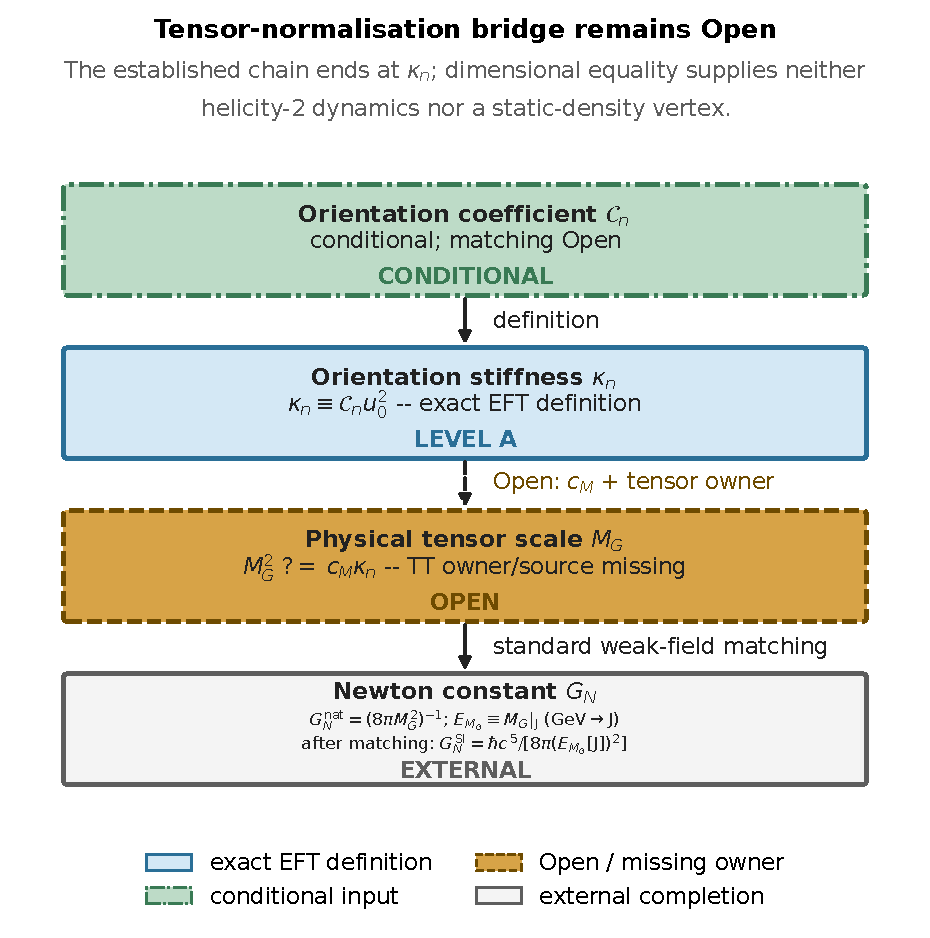
\includegraphics[width=0.94\textwidth,height=0.68\textheight,keepaspectratio]{figures/r177/global/panels/fig41_b_tensor_normalisation_terminal_units_r177.pdf}
\caption{Corrected ownership chain from the ordered variables through the
conditional NLO orientation coefficient and the exact EFT definition
$\kappa_n\equiv\mathcal C_nu_0^2$.  The dashed step
$M_G^2\stackrel{?}{=}c_M\kappa_n$ is Open: the physical helicity--2 action,
source normalisation, residue and the coefficient $c_M$ are not supplied.
The natural-unit tensor normalisation
$G_N^{\rm nat}=(8\pi M_G^2)^{-1}$ is standard only inside a supplied tensor
completion.  An SI Newton constant is defined only after physical tensor,
source, clock, light and scalar-response matching, as
$G_N^{\rm SI}=\hbar c^5/[8\pi(E_{M_G}[\mathrm J])^2]$, where
$E_{M_G}\equiv M_G|_{\rm joule}$ denotes the manuscript energy scale converted
from GeV to joules.  Colour is redundant with
fill luminance, border style, arrow style and literal status text.  The diagram
therefore does not derive gravity from $\kappa_n$.  Complementary full-width
panels are retained in Appendix~\ref{app:r129_visual_orientation_tensor}.}
\label{fig:r103_Cn_scalechain_corrected}
\end{figure}

\subsection{Phase sector and action scale}
\label{app:dim_phase}
The action scale $S_0$ and its matching to $\hbar$ are independent of the Open
tensor-normalisation bridge.

\paragraph{Three distinct response levels.}
\label{par:two_level_consistency}
The scalar principal tensor, an orientation stiffness and a physical tensor
coefficient are different operator owners.  A dimensionless derivative
expansion diagnostic, after normalising the leading operator, is for example
\begin{equation}
\label{eq:NLO_suppression}
\epsilon_n(k)=|\mathcal C_n|\,k^2\ll1 .
\end{equation}
The former quantity
$c_M\mathcal C_nu_0^2/c_{\rm char}^2$ had mass dimension two and was not a
suppression factor; it is withdrawn.

\subsection{Owner chain}
\label{app:dim_summary}
The established chain ends at the orientation operator:
\[
\partial_A\Phi=un_A
\longrightarrow \mathcal C_n
\longrightarrow \kappa_n=\mathcal C_nu_0^2.
\]
The continuation $\kappa_n\to M_G^2\to G_N$ is Open at its first arrow; the
second is standard weak-field matching inside a supplied tensor/Einstein EFT.

\subsection*{Detailed derivation and matching inventory}

\paragraph{Canonical dimensions.}
In four Euclidean dimensions a canonically normalised scalar has mass
dimension one, its gradient has dimension two, and the ordered-gradient
amplitude $u$ therefore has dimension two.  The unit director $n_A$ is
dimensionless.  The operator $u^2(\partial n)^2$ has dimension six, so its
Wilson coefficient $\mathcal C_n$ has dimension minus two and
$\kappa_n=\mathcal C_nu_0^2$ has dimension two.  This audit establishes the
orientation stiffness and nothing about its particle representation.

\paragraph{Why leading $P(X)$ is insufficient.}
For a one-scalar pullback $Q_A=\partial_A\Phi=un_A$, the exact integrability
condition $\partial_{[A}Q_{B]}=0$ relates director gradients to amplitude
gradients.  A pure local $P(X)$ action depends algebraically on $Q_AQ^A$ and
does not generate an independent two-derivative director elasticity at tree
level.  Such an operator must arise from higher derivatives, additional
fields, loops, boundaries or a declared nonlocal reduction.  This identifies
the derivative order but not a tensor-gravity owner.

\paragraph{Conditional heavy-amplitude determinant.}
Expanding $u=u_0+\sigma$ around the ordered background gives a massive radial
operator of Laplace type only after the background, measure and constraint
reduction are fixed.  Formally integrating the radial field produces
$\Gamma_\sigma=\tfrac12\operatorname{Tr}\ln\mathcal O_\sigma$.  A proper-time
or heat-kernel expansion then organises local operators in powers of
$1/m_\sigma$.  The coefficient multiplying a two-derivative orientation
invariant is scheme- and basis-dependent; power divergences, logarithms and
finite counterterms must be declared.  P4 supplies neither this operator nor
its mass; identifying $m_\sigma$ with the homogeneous-P3 curvature or a
Planck-scale pole is a separate matching ansatz.

\paragraph{Foliation geometry.}
When the director defines codimension-one leaves, its projected symmetric
derivative can be organised as an extrinsic-curvature tensor only after the
normal, projector and integrability assumptions are supplied.  The exact
pointwise relation is Eq.~\eqref{eq:gauss_embedding_scoped}: the leaf Ricci
scalar equals the projected ambient Riemann contraction plus
$\epsilon(K^2-K_{ab}K^{ab})$.  In the Euclidean convention
$\epsilon=+1$, and flat ambient geometry removes only the projected ambient
term.  Boundary divergences enter a scalar-curvature action decomposition,
not this identity.  Neither $K^2-K_{ab}K^{ab}$ nor the Ricci scalar is
identically $(\partial n)^2$; the general local basis contains independent
trace, traceless, acceleration and boundary operators.  Reduction to one
coefficient $\mathcal C_n$ therefore requires a trace constraint,
integration-by-parts identity, boundary condition or matching prescription.
This ambiguity is physical and cannot be hidden in a notation change.

\paragraph{Conditional leaf-conformal kernel.}
If one deliberately chooses a scalar Laplace-type operator on
three-dimensional leaves with conformal coefficient
$\xi_{\rm leaf}=1/8$, the standard curvature coefficient contains
$1/6-\xi_{\rm leaf}=1/24$.  That arithmetic is exact under the declared
closure.  It fixes only a geometric factor in one curvature channel.  It does
not fix the finite Wilson coefficient, the reduction to $(\partial n)^2$, or
the normalisation of a physical tensor pole.  The factor $1/24$ must therefore
remain conditional rather than being presented as a Planck-scale prediction.

\paragraph{Renormalised coefficient.}
The parametrisation
\[
\mathcal C_n=\frac{\hat a_{\rm eff}}{16\pi^2m_\sigma^2},
\qquad
\hat a_{\rm eff}=\gamma_{\rm fol}\mathcal N_{\rm match},
\]
separates the loop scale from a finite matched normalisation.  The symbol
$\mathcal N_{\rm match}$ includes regulator-dependent pieces, operator-basis
reduction and finite counterterms.  It must not include a hidden spin-2
identification: the latter is a separate map from the orientation Hessian to
a physical constrained tensor residue.

\paragraph{What the one-loop route actually establishes.}
Under its assumptions, the radial determinant makes an NLO orientation
operator plausible and supplies a reproducible power-counting form.  It does
not establish the sign or numerical size of the complete renormalised
coefficient without a UV prescription.  More importantly, it changes a
coefficient of the orientation EFT; it does not change the fixed-$\alpha,\beta$
tangent-director linear theorem $h_{ij}^{\rm TT}=h_{ww}=0$ or create a
linear static-density vertex.  Quadratic/nonlinear response remains a
separate parametric/Open question.

\paragraph{Open tensor map.}
To relate $\kappa_n$ to a tensor normalisation, one must enlarge or alter the
field map, derive the constrained quadratic operator, isolate a symmetric
physical pole and compute its residue.  Only then is a coefficient $c_M$ in
$M_G^2=c_M\kappa_n$ meaningful.  Setting $c_M=1$ by convention before that
calculation is not weak-field matching; it is an unsupported identification.

\paragraph{Weak-field calibration.}
Given a supplied Einstein/FP tensor action, the observed $G_N$ calibrates its
coefficient $M_G$.  This calibration may be used to infer what value of a
microscopic combination would be required, but the inference is not a
prediction of that combination.  A large value of
$\mathcal N_{\rm match}$ or $c_M$ is a naturalness diagnostic, not evidence
that the missing tensor map has been derived.

\paragraph{Phase action scale remains separate.}
The phase stiffness, fixed-core coefficient $\iota_0^{\rm EFT}$ and
positive-tension coefficient $\iota_{0,\rm bal}^{\rm eff}$ belong to supplied
compact-phase loop models.  Their dimensional reduction, either map to the
operational $S_0$, and the separate matching $S_0\leftrightarrow\hbar$ do
not determine $M_G$.  Conversely, calibrating
$M_G$ with $G_N$ does not derive $S_0$.  Common origin in one condensate does
not collapse independent Wilson coefficients into one parameter.

\paragraph{Three response levels.}
The manuscript therefore distinguishes: (i) the leading scalar principal
tensor and its cone; (ii) an NLO orientation stiffness; and (iii) a possible
physical tensor coefficient.  These are different operator owners.  The
diagnostic ratio in Eq.~\eqref{eq:NLO_suppression} is dimensionally valid, but
it becomes gravitational only after the Open coefficient and tensor map are
derived.

\paragraph{Reproducibility requirements.}
A future closure of this appendix must provide the expanded radial operator,
constraint Jacobian, boundary conditions, regularisation and subtraction
scheme, complete foliation-invariant operator basis, finite Wilson
coefficients, constrained pole decomposition, tensor projector and matter
vertex.  The calculation should be reproducible both in the Euclidean parent
description and in the reduced Lorentzian EFT.  Until then the complete
established chain ends at $\kappa_n$.

\section{Correlation Length from the Radial-Mode Propagator}
\label{app:corr_length}

\textit{Reference from main text: Section~\ref{sec:sigma_scales}.
Status: standard EFT estimate from the massive Euclidean propagator.}

\subsection*{Euclidean propagator}

Quadratic action of the radial mode:
$S_\sigma^{(2)}=\frac{1}{2}\int d^4X[(\partial_A\sigma)^2+m_\sigma^2\sigma^2]$.
Fourier propagator: $G_\sigma(k)=1/(k^2+m_\sigma^2)$.

\subsection*{Coordinate representation at large distances}

In $d=4$ Euclidean space the exact free propagator and its
large-distance asymptotic are
\begin{equation}
  \label{eq:G_coord}
  G_\sigma(r)=\frac{m_\sigma}{4\pi^2r}K_1(m_\sigma r)
  \;\xrightarrow{m_\sigma r\to\infty}\;
  \frac{\sqrt{m_\sigma}}{4\sqrt{2}\,\pi^{3/2}}\,
  \frac{e^{-m_\sigma r}}{r^{3/2}}.
\end{equation}
The exponential factor $e^{-m_\sigma r}$ defines the P3 homogeneous
radial decay length
\begin{equation}
  \boxed{\xi_{\rm P3}=m_{\Phi,\mathrm{rad}}^{-1}.}
\end{equation}
This is standard P3 free-field mathematics.  It is not a P4 correlation
length or ordered-branch threshold; both that owner map and any Planck-length
matching remain Open.

% ------------------------------------------------------------
\section{Phase Periodicity, Winding Sectors, and the Fixed-Core Coefficient $\iota_0^{\rm EFT}$}
\label{app:action_scale_S0}

\textit{Reference from main text: Section~\ref{sec:hbar_status}.
Status: Level~A mathematics for the supplied dimensionless fixed-core
evaluation; Level~B route / Open physical owner and matching.
The compact phase and its periodicity belong to the $U(1)$-extended phase EFT
(modelling step beyond bare~P3).  The independent positive action factor
$\Sigma_\theta$, its owner, and any map
$\Sigma_\theta\iota_0^{\rm EFT}\to S_0\leftrightarrow\hbar$ are not derived.}

This appendix makes explicit the chain behind the candidate map
$\Sigma_\theta\iota_0^{\rm EFT}\to\hbar$.  Its purpose is not to derive the
full quantum formalism: the supplied $U(1)$/fixed-core extension produces a
dimensionless reduced coefficient, while an independent finite positive
$\Sigma_\theta$ is required before an action-valued product exists.
It should be noted that the real scalar field $\Phi$ of P3 does not
by itself carry a compact $U(1)$ phase variable; the
extension to $\Phi_{\rm eff}=\rho\,e^{i\theta}$ is an additional
modelling step for the coherent sector, not a direct topological
consequence of the supplied orientation orbit $O(4)/O(3)\simeq S^3$
(which has $\pi_1(S^3)=0$).

\subsection*{A.\ Phase variable on the coherent branch}

Let the coherent collective state be described by a phase-like
variable $\theta$.
Because physically equivalent coherent states are identified after
a full winding, the phase lives on a circle:
\begin{equation}
  \theta \in S^1, \qquad \theta \sim \theta + 2\pi.
  \label{eq:app_theta_circle}
\end{equation}
This is the minimal topological statement behind the coherent winding
sector~(BR1).

\subsection*{B.\ Optional action--angle parametrisation}

A phase is dimensionless.  If one separately supplies a multivalued
action--angle coordinate $\mathscr S$ with an action scale $S_{\rm ph}$, one
may write the Level~B/Open map
\begin{equation}
  \theta = \frac{\mathscr S}{S_{\rm ph}},
  \label{eq:app_theta_S_ratio}
\end{equation}
and hence
\begin{equation}
  e^{i\theta} = \exp\!\left(i\frac{\mathscr S}{S_{\rm ph}}\right).
  \label{eq:app_phase_factor}
\end{equation}
This is not an identity between the angular coordinate and the single-valued
Euclidean phase-gradient functional $\mathcal I_{\rm loop}[\theta]$.  The canonical
pair, monodromy and owner of $S_{\rm ph}$ must be derived or supplied.

\subsection*{C.\ Winding and the fixed-core evaluation}

For a supplied closed one-dimensional carrier, single-valuedness requires
\begin{equation}
  \oint d\theta = 2\pi n, \qquad n\in\mathbb{Z}.
  \label{eq:app_winding_number}
\end{equation}
Only under the separate action--angle assumption~\eqref{eq:app_theta_S_ratio}
does this imply the monodromy
\begin{equation}
  \oint d\mathscr S = 2\pi n\,S_{\rm ph}.
  \label{eq:app_action_loop_quantisation}
\end{equation}
It does not identify the value of the phase-gradient functional: for a
uniform winding, $\mathcal I_{\rm loop}$ is constant after a circuit even though
$\oint d\theta=2\pi n$.  The supplied fixed-core representative is instead
defined by evaluating the fixed-$L$ functional of
Eq.~\eqref{eq:loop_bound} at $n=1$ and $L=L_{\rm core}$:
\begin{equation}
  \iota_{\rm elem}^{\rm(fixed\ core)}
  :=\mathcal I_{\rm loop}[\theta_{\rm unif};L_{\rm core}]
  =\frac{2\pi^2K_\theta^{1\mathrm D}}{L_{\rm core}}
  =2\pi \iota_0^{\rm EFT}.
  \label{eq:app_min_action_loop}
\end{equation}
The last equality is the fixed-core coefficient definition, not a topological
quantisation of the full action.

\subsection*{D.\ Status of the identification with $\hbar$}

The correspondence $\hbar \leftrightarrow \Sigma_\theta\,\iota_0^{\rm EFT}$ should be understood
as follows.
What is established is only that a supplied compact-phase/fixed-core EFT may
contain the dimensionless reduced coefficient $\iota_0^{\rm EFT}$ obtained
from its phase-gradient functional, while winding organises integer sectors.
The candidate physical coefficient is the independent product
$\Sigma_\theta\iota_0^{\rm EFT}$.  A separate
action--angle map may use an action scale, but topology does not fix that
scale, a nonzero physical value, or its universality.  The candidate-to-operational map
$\Sigma_\theta\,\iota_0^{\rm EFT}\to S_0$ remains Open because the physical
operator/state map and cross-sector normalisation are not derived.  The final
equality $S_0=\hbar$ is separately adopted as a Level-B physical calibration;
its microscopic explanation and universality remain Open.

\subsection*{E.\ Summary}

The coherent branch provides:
\begin{enumerate}
  \item a periodic phase variable~\eqref{eq:app_theta_circle};
  \item integer winding sectors~\eqref{eq:app_winding_number};
  \item a fixed-core representative obtained by evaluating the supplied
    phase-gradient functional after the core length and EFT coefficient are
    supplied, not from winding alone;
  \item an optional action--angle analogy whose canonical owner is Open;
  \item an Open owner programme for
    $\Sigma_\theta\,\iota_0^{\rm EFT}\to S_0$, followed by the separately
    adopted Level-B calibration $S_0=\hbar$; neither step is a derivation of
    the calibration's microscopic origin.
\end{enumerate}

% ------------------------------------------------------------
\section{Noether Currents: Translational and Rotational Sectors}
\label{app:noether_full}

\textit{Reference from main text: Section~\ref{sec:noether}.
Status: classical field theory; no quantisation required.}

\subsection*{A. Translational invariance and $T^{AB}$}

\noindent\textbf{Scalar bare sector~(P3):}
\begin{equation}
  \tau_{\rm P3}^{AB}
  =\partial^A\Phi\,\partial^B\Phi
   -\delta^{AB}\!\left[\tfrac12(\partial_C\Phi)^2+V(\Phi)\right],
  \qquad
  \partial_A\tau_{\rm P3}^{AB}
  =-\frac{\delta\mathcal I_E^{\rm P3}}{\delta\Phi}\partial^B\Phi,
  \qquad
  T_{{\rm P3},{\rm phys}}^{AB}=A_{\rm P3}\tau_{\rm P3}^{AB}.
\end{equation}
The reduced and physical currents have the same on-shell conservation law
for constant $A_{\rm P3}>0$.  The path-integral denominator
$\Sigma_{\rm PI,P3}$ and ratio $\kappa_{\rm P3}$ control the supplied
Euclidean measure, not this physical-current prefactor.

\noindent\textbf{Orientation sigma-model~\eqref{eq:sigma_model}:}
\begin{equation}
\begin{aligned}
  T^{AB}_{(n)}
  &=\kappa_n\,\partial^A n_C\,\partial^B n^C
    -\delta^{AB}\tfrac{\kappa_n}{2}(\partial_D n_E)^2,\\
  \partial_AT^{AB}_{(n)}
  &=-\frac{\delta S_n}{\delta n_C}\,\partial^B n_C,\\
  \partial_AT^{AB}_{(n)}
  &=0\qquad\text{on the sigma-model shell}.
\end{aligned}
\end{equation}
These local on-shell identities follow from translation invariance of their
respective owning actions, not from homogeneity or $O(4)$ rotations.
Boundary assumptions enter differentiable generators and conserved
integrated charges.

\subsection*{B. $O(4)$-invariance and angular currents}

For the P3 $O(4)$-invariant scalar action, Noether's
theorem~\cite{Noether1918} for
$\delta X^A=\omega^A{}_BX^B$ gives
\begin{equation}
  j_{\rm P3}^{C,AB}
  =X^A\tau_{\rm P3}^{CB}-X^B\tau_{\rm P3}^{CA},\qquad
  J_{{\rm P3},{\rm phys}}^{C,AB}=A_{\rm P3}j_{\rm P3}^{C,AB},
  \qquad
  \partial_Cj_{\rm P3}^{C,AB}
  =\partial_CJ_{{\rm P3},{\rm phys}}^{C,AB}=0
\end{equation}
only on the P3 equations of motion.  Off shell its divergence is the
corresponding Euler--Lagrange combination.  Admissible boundaries are
additionally required for a differentiable generator and conserved
integrated angular charge.
For the orientation field $n_A$ (a vector under $O(4)$),
a spin contribution is added:
\begin{equation}
  J^{C,AB}_{(n)}=X^A T^{CB}_{(n)}-X^B T^{CA}_{(n)}
  +\kappa_n(n^A\partial^C n^B-n^B\partial^C n^A).
\end{equation}

\subsection*{C. Currents under a declared branch restriction}

The translational and rotational currents above belong to the bare real-scalar
P3 action.  A branch-restricted action inherits them only when the restriction,
boundary data, and allowed variations preserve the corresponding symmetry.
Separately supplied branch EFTs own their own currents; their existence does
not follow from the bare-current formulas alone.

% ------------------------------------------------------------
\section{Variational Stationarity and Reduced Extremal Dynamics}
\label{app:variational_reduction}

\textit{Reference from main text:
Section~\ref{sec:noether}.
Status: schematic reduction programme at Level~B/Open.  Variation inside an
explicitly supplied reduced action is exact for that owner, while descent from
DP remains Open until a variation-compatible restriction or controlled
elimination is derived.}

This appendix records the conditions under which medium-level
stationarity may descend to a branch effective action.  It does not assume a
universal chain: an explicit variation-compatible restriction or controlled
elimination is required in each case.

\paragraph{Step 1. Medium extremality.}
By DP, every physically realised configuration must satisfy the necessary
stationarity condition
\begin{equation}
  \delta S_E[\Phi] = 0.
  \label{eq:app_medium_ext}
\end{equation}

\paragraph{Step 2. Branch decomposition.}
In the ordered branch, decompose the full field into background and
fluctuations:
\begin{equation}
  \Phi = \Phi_{\rm branch} + \delta\Phi,
\end{equation}
where $\Phi_{\rm branch}$ specifies the ordered background~(P4) and
$\delta\Phi$ denotes fluctuations over it.

\paragraph{Step 3. Conditional construction of a reduced functional.}
A branch decomposition does not by itself define an effective action.  One
must either impose a consistent restriction of $S_E$ or integrate out declared
modes with the measure, boundary data, constraints, and induced terms tracked.
Only for such a variation-compatible map $R$ may one prove
\begin{equation}
  \delta S_E[\Phi]\big|_{R}=0
  \quad\Longrightarrow\quad
  \delta S_{\rm eff}[\psi_i]=0
  \qquad\text{for the variations preserved by $R$}.
  \label{eq:app_branch_ext}
\end{equation}
An EFT action introduced independently is instead its own conditional owner;
matching its coefficients does not prove the implication above.

\paragraph{Step 4. Interpretation and status.}
Equation~\eqref{eq:app_branch_ext} is therefore a Level~A conditional
variational statement once a particular compatible map $R$ is derived.  The
existence of such maps for all phase, gauge, fermion, gravity, cosmology, HRC,
and open-system actions displayed in this manuscript is Open.  Lorentzian
stationary-phase dominance additionally requires its own oscillatory measure,
contour, state, Hessian and boundary data, and does not follow from
Eq.~\eqref{eq:app_branch_ext}.  No universal DP-to-EFT-to-macroscopic descent
chain is asserted.

% ------------------------------------------------------------
\section{Noether current and local $U(1)$ completion in the compact phase EFT}
\label{app:u1_noether_completion}
% ============================================================

This appendix collects the explicit derivations underlying the
$U(1)$ gauge construction of Section~\ref{sec:u1_emergence}.

\subsection*{A.\ Global phase symmetry and Noether current}

Let
$\Phi_{\rm eff}(X)=\rho(X)e^{i\theta(X)}$,
with effective Lagrangian
\begin{equation}
  \mathcal{L} = \partial_A\Phi_{\rm eff}^*\partial^A\Phi_{\rm eff}
  - V(|\Phi_{\rm eff}|).
\end{equation}
Under the infinitesimal global transformation
$\delta\Phi_{\rm eff}=i\alpha\Phi_{\rm eff}$,
$\delta\Phi_{\rm eff}^*=-i\alpha\Phi_{\rm eff}^*$,
Noether's theorem gives
\begin{equation}
  j^A=
  \frac{\partial\mathcal{L}}{\partial(\partial_A\Phi_{\rm eff})}
  \,\delta\Phi_{\rm eff}
  +
  \frac{\partial\mathcal{L}}{\partial(\partial_A\Phi_{\rm eff}^*)}
  \,\delta\Phi_{\rm eff}^*.
\end{equation}
Since
$\partial\mathcal{L}/\partial(\partial_A\Phi_{\rm eff})
=\partial^A\Phi_{\rm eff}^*$
and
$\partial\mathcal{L}/\partial(\partial_A\Phi_{\rm eff}^*)
=\partial^A\Phi_{\rm eff}$,
one obtains
\begin{equation}
  j^A=
  i\alpha\left(
  \partial^A\Phi_{\rm eff}^*\,\Phi_{\rm eff}
  -\partial^A\Phi_{\rm eff}\,\Phi_{\rm eff}^*
  \right).
\end{equation}
Removing the overall infinitesimal parameter and adopting the standard
normalisation yields
\begin{equation}
  j^A=
  \frac{-i}{2}\left(
  \Phi_{\rm eff}^*\partial^A\Phi_{\rm eff}
  -\Phi_{\rm eff}\partial^A\Phi_{\rm eff}^*
  \right).
\end{equation}
Substituting $\Phi_{\rm eff}=\rho e^{i\theta}$:
\begin{equation}
  j^A=\rho^2\partial^A\theta.
\end{equation}

\subsection*{B.\ Necessity of the compensating connection under local phase redefinition}

Under
$\Phi_{\rm eff}(X)\to e^{i\alpha(X)}\Phi_{\rm eff}(X)$,
the derivative transforms as
\begin{equation}
  \partial_A\Phi_{\rm eff}\to
  e^{i\alpha(X)}\!\left(\partial_A\Phi_{\rm eff}
  +i(\partial_A\alpha)\Phi_{\rm eff}\right).
\end{equation}
The inhomogeneous term $i(\partial_A\alpha)\Phi_{\rm eff}$
prevents covariance.
Introduce a field $A_A$ with transformation
$A_A\to A_A+\frac{1}{e}\partial_A\alpha$.
Then
\begin{equation}
  D_A\Phi_{\rm eff}\equiv(\partial_A-ieA_A)\Phi_{\rm eff}
\end{equation}
transforms covariantly:
$D_A\Phi_{\rm eff}\to e^{i\alpha(X)}D_A\Phi_{\rm eff}$.

\subsection*{C.\ Leading kinetic term}

The antisymmetric combination
$F_{AB}=\partial_AA_B-\partial_BA_A$
is gauge invariant.
On a supplied ordered background the leading local parity-even quadratic
basis contains two invariants,
$I_1=F_{AB}F^{AB}$ and
$I_2=(n^AF_{AB})(n_CF^{CB})$, up to normalisation and total derivatives.
Thus the general leading action is
\begin{equation}
  S_{\rm gauge}=-\frac14\int d^4X\,[Z_1I_1+2Z_2I_2].
\end{equation}
The Maxwell form is the special isotropic choice $Z_2=0$; P5 alone does
not impose it.  Coefficients, signs, reduced Hessian and physical photon
matching remain Open.

\subsection*{D.\ Compact phase, local gauge completion, and holonomy}

For compact $\theta\sim\theta+2\pi$, the gauge-invariant phase
gradient is
$\mathcal{D}_A\theta=\partial_A\theta-eA_A$.
Single-valuedness around a closed loop $\gamma$ implies only
\begin{equation}
  \oint_\gamma \partial_A\theta\,dX^A=2\pi n,
  \qquad n\in\mathbb{Z}.
\end{equation}
Consequently the covariant circulation is
\begin{equation}
  \oint_\gamma \mathcal D_A\theta\,dX^A
  =2\pi n-e\oint_\gamma A_A\,dX^A.
\end{equation}
Flux quantisation follows only after the additional equilibrium or
zero-covariant-circulation condition
$\oint_\gamma\mathcal D_A\theta\,dX^A=0$ is imposed.  It is therefore a
conditional property of the supplied local completion, not a consequence of
single-valuedness alone.


% ============================================================
\section{Non-Abelian local completion and the
\texorpdfstring{$\mathfrak{so}(3)\cong\mathfrak{su}(2)$}{so(3)=su(2)} bridge}
\label{app:nonabelian_completion}
% ============================================================

This appendix records the explicit structural steps behind
Section~\ref{sec:nonabelian_embedding}.

\subsection*{A.\ Local multiplet completion}

Let $\Phi$ be an $N$-component effective condensate multiplet.
Suppose the effective action is invariant under global
$SU(N)$ transformations
\begin{equation}
  \Phi\to U\Phi,
  \qquad U\in SU(N).
\end{equation}
If one promotes $U$ to a local transformation $U(X)$, covariance
of derivatives requires the introduction of a Lie-algebra-valued
connection
\begin{equation}
  A_A = A_A^a T^a,
\end{equation}
with covariant derivative
\begin{equation}
  D_A=\partial_A-igA_A.
\end{equation}
This is the standard local completion of a global multiplet symmetry.

\subsection*{B.\ Field strength from commutator closure}

Demanding that the covariant derivatives close under commutation gives
\begin{equation}
  [D_A,D_B]\Phi = -ig\,F_{AB}\Phi,
\end{equation}
with
\begin{equation}
  F_{AB}=\partial_AA_B-\partial_BA_A-ig[A_A,A_B].
\end{equation}
In component form this yields
\begin{equation}
  F_{AB}^a=\partial_AA_B^a-\partial_BA_A^a+g f^{abc}A_A^bA_B^c.
\end{equation}
Thus the commutator term is forced by local non-Abelian covariance.

\subsection*{C.\ Leading ordered-background kinetic basis}

At leading derivative order, a supplied ordered director allows two local
parity-even quadratic invariants,
\begin{equation}
  I^{\rm NA}_1=F_{AB}^aF^{a\,AB},\qquad
  I^{\rm NA}_2=(n^AF_{AB}^a)(n_CF^{a\,CB}),
\end{equation}
up to normalisation and total derivatives.  The general residual-$O(3)$
action therefore has independent coefficients multiplying both invariants.
The canonical isotropic Yang--Mills action is recovered only if a stronger
symmetry or matching condition sets the second coefficient to zero; neither
P5 nor local gauge covariance alone does so.

\subsection*{D.\ The $\mathfrak{so}(3)\cong\mathfrak{su}(2)$ bridge}

The Lie algebra $\mathfrak{so}(3)$ has generators $J_i$ obeying
\begin{equation}
  [J_i,J_j]=\epsilon_{ijk}J_k.
\end{equation}
The Lie algebra $\mathfrak{su}(2)$ has generators $T_i$ obeying
\begin{equation}
  [T_i,T_j]=\epsilon_{ijk}T_k
\end{equation}
up to conventional normalisation.
Hence
\begin{equation}
  \mathfrak{so}(3)\cong\mathfrak{su}(2).
\end{equation}
This is an isomorphism of Lie algebras only.
It does not imply that the global groups $SO(3)$ and $SU(2)$ are
identical, nor does it by itself determine the physical matter
representation content.

\subsection*{E.\ Limit of the argument}

This appendix derives the standard connection, curvature and
two-invariant kinetic-basis algebra only after a local multiplet redundancy,
bundle and action have been supplied.  It also records the exact Lie-algebra
isomorphism $\mathfrak{so}(3)\simeq\mathfrak{su}(2)$.  It does not derive a
physical gauge bundle from P1--P6, select canonical Yang--Mills/Maxwell
($Z_2=0$), or derive Standard-Model representations, couplings, confinement
or electroweak breaking.


% ============================================================
\section{Conditional operator classification and missing matching owner for the
fermion--director coupling}
\label{app:fifth_operator_classification}
% ============================================================

This appendix records the explicit EFT logic behind
Section~\ref{sec:fifth_coupling}.

\subsection*{A.\ Bilinear basis}

The standard local fermion bilinears are
\[
\bar\Psi\Psi,\qquad
\bar\Psi i\gamma^5\Psi,\qquad
\bar\Psi\gamma^A\Psi,\qquad
\bar\Psi\gamma^A\gamma^5\Psi,\qquad
\bar\Psi\sigma^{AB}\Psi.
\]
To form a scalar interaction linear in the preferred direction $n_A$,
the natural zeroth-derivative candidates are
\[
n_A\bar\Psi\gamma^A\Psi,
\qquad
n_A\bar\Psi\gamma^A\gamma^5\Psi.
\]
If one restricts attention to the parity-even EFT sector, the axial
candidate is excluded and the vector operator remains as the leading
allowed term.

\subsection*{B.\ Why the vector operator is leading}

Derivative couplings such as
\[
n_A\bar\Psi\sigma^{AB}\partial_B\Psi,
\qquad
(\partial_A n_B)\bar\Psi\sigma^{AB}\Psi
\]
are higher-order in the derivative expansion and are therefore
subleading in the low-energy EFT.
Accordingly, within the parity-even, zeroth-derivative basis, the
leading ECT-specific operator is
\[
n_A\bar\Psi\gamma^A\Psi.
\]

\subsection*{C.\ Dimensional analysis}

In four spacetime dimensions the fermion field has mass dimension
\[
[\Psi]=\frac32,
\]
so the bilinear
\[
\bar\Psi\gamma^A n_A\Psi
\]
has dimension three.
Therefore the coefficient multiplying it in the Lagrangian density must
have mass dimension one:
\[
[\mu_5]=1.
\]
This is why the coefficient should not be treated as purely
dimensionless at the Lagrangian level.

\subsection*{D.\ Dimensionless parameterisation and missing scale}

A possible parameterisation is
\[
\mu_5=\beta_5 m_f,
\]
where $\beta_5$ is dimensionless.
Dimensions alone do not select $\beta_5$, a nonzero coefficient, its sign,
mass dependence, suppression scale or species dependence.  No numerical
benchmark is retained.

\subsection*{E.\ Lorentzian reduction and observability caveat}

In the Lorentzian ordered branch, the preferred Euclidean direction
induces a timelike vector $u_\mu$, and the operator becomes
\[
\mu_5\,u_\mu\bar\Psi\gamma^\mu\Psi.
\]
For a constant background and a single fermion species, such a term can
be partly removed by field redefinitions.
Hence the physical content of the coupling is tied to relative effects,
species dependence, gradients, or environmental variation of the ordered
branch.
This explains why the structural admissibility of the operator is
stronger than the current proof of its directly observable low-energy
effects.

The distinction among this microscopic operator, the Level-B scalar
ansatz, and the supplied conditional HRC gravity functional is recorded in
Appendix~\ref{app:fifth_micro_macro}.

% ============================================================
\section{Microscopic operator, scalar ansatz, and galactic functional}
\label{app:fifth_micro_macro}

This appendix records three objects rather than two versions of one
mechanism.

\subsection*{M --- microscopic preferred-direction operator}
\[
M:\qquad \Delta\mathcal L_5=\mu_5\bar\Psi\gamma^A n_A\Psi,
\qquad [\mu_5]=1.
\]
Its operator classification is A/B conditional; its coefficient and
observable multi-species reduction are Open.

\subsection*{S --- scalar response ansatz}
\[
S:\qquad \phi_u=\beta_\phi^{-1}\ln(u/u_\infty),
\qquad F(\phi_u)=u/u_\infty.
\]
This Level-B ansatz yields conditional local scalar identities.  It does not
yet yield a body charge, screening profile, or galactic force law.

\subsection*{G --- conditional HRC gravity functional}
\[
G:\qquad \mu_{g,k}(g^2/a_M^2)g=g_N.
\]
Its response algebra is Level~A inside the supplied augmented model; the
identity/microscopic bridge is Level~B/Open and the fits are Level~C.  The fit arithmetic does not identify
its physical scalar coordinate or derive its source/force normalisation.

The strict result is M$\neq$S by variable/operator content.  The relation
S$\to$G is an Open matching problem and must be represented by a dashed edge.
No statement here derives all three from a common branch-level response.

% ============================================================
\section{Dimensional scaling and open condensate-scale assignments
for the preferred-direction coefficient}
\label{app:fifth_coefficient_scales}
% ============================================================

This appendix records the scale argument behind
Section~\ref{sec:fifth_coefficient_constraints}.

\paragraph{A.\ Operator dimension.}
The operator
\[
\bar\Psi\gamma^A n_A\Psi
\]
has mass dimension three in four dimensions.
Its coefficient must therefore have mass dimension one.

\paragraph{B.\ Available scales.}
In the present ECT architecture, the preferred direction $n_A$ is a
normalised-gradient variable on the adopted P4 chart.  P4 postulates the
physically relevant ordered branch; its stationary action, transition and
dynamical formation/selection mechanism remain Open.  Several scales are nevertheless
present: the gradient order parameter $u_0$, the radial/Planck-scale
parameter $\phi_0$ associated with the symmetry-breaking amplitude of the
bare potential, and the later electroweak-like scale $v_2$.

\paragraph{C.\ Consequence.}
Dimensional analysis establishes only $[\mu_5]=1$.  The available scales do
not select a nonzero coefficient or a monomial dependence on $m_f$,
$\phi_0$, $u_0$ or $v_2$.  The choices $\mu_5=0$ and arbitrary
dimension-one matching functions are direct counterexamples to any unique
species-scaling inference.

\paragraph{D.\ Open owner.}
A value or species law for $\mu_5$ requires a physical fermion action,
representations, matching calculation and radiative closure.  None is
derived, so no preferred suppression scale is assigned.

\section{$\phi$-first nonlinear gravity: complete derivation inside the supplied IR closure}
\label{app:phi_first_EFE}
% ============================================================

This appendix gives the complete derivation internal to the supplied
$\phi$-first scalar--tensor IR closure, states its conditional theorems
precisely, and compares its equations with analogous equations in related
theories.  It does not derive that closure from P1--P6 or establish a physical
ECT metric completion.

% -----------------------------------------------------------
\subsection*{A.1 Theorem A: Allowed quadratic scalar tensor and its
conditional principal cone}
% -----------------------------------------------------------

\textbf{Statement.}
On the ordered branch, the most general leading quadratic $O(3)$-invariant
symmetric rank-2 scalar kinetic tensor has the two-parameter form
\begin{equation}
  K^{AB} = \beta\,\delta^{AB} - \alpha\,n^A n^B.
  \label{eq:K_unique}
\end{equation}
Once this second-order scalar operator is supplied, it has one scalar
principal polynomial and, in the hyperbolic window, one conditional scalar
principal cone.  The symmetry classification does not by itself supply a
physical action, exclude higher-order principal factors, or derive universal
metric coupling.  The latter is assumption~A4 (IR closure assumption; not
proved beyond linear order).

\textbf{Proof.}
Any $O(3)$-invariant symmetric rank-2 tensor built from
$\{\delta^{AB}, n^A\}$ has the form $T^{AB}=a\,\delta^{AB}+b\,n^An^B$
with two scalars $a,b$.  Matching the displayed operator gives
$a=\beta$, $b=-\alpha$; hence
$K^{ij}=\beta\delta^{ij}$ and
$K^{ww}=\beta-\alpha=-\Delta_K$ on $n^A=\delta^A_w$.
No other independent structure exists. $\square$

% -----------------------------------------------------------
\subsection*{A.2 Lemma B: conditional logarithmic parameterisation}

For any scalar--tensor closure with positive non-minimal factor $f(q)$,
\begin{equation}
  \psi_f(q)\equiv\ln\frac{f(q)}{f_0},
  \qquad f(q)=f_0e^{\psi_f(q)},
\end{equation}
is an exact algebraic reparameterisation.  In the amplitude-dominated
closure one further assumes
$f/\bar M_{\rm Pl}^2=u/u_\infty=e^{\beta_\phi\phi_u}$, so that
$\psi_f=\beta_\phi\phi_u$.  This latter identification is Level~B matching,
not an algebraic theorem from bare P3.

The anisotropy variable $\Delta_K=\alpha-\beta$ is distinct.  Defining
$\psi_K=\ln(\Delta_K/\Delta_{K,{\rm vac}})$ is separately algebraic, but no
$u\leftrightarrow\Delta_K$ map has been derived.  The two logarithmic variables
must not be identified without that missing bridge.

\subsection*{A.3 Proposition C: scalar-only IR action (effective ansatz)}

$S_{\rm IR}$ in Eq.~\eqref{eq:phi_first_action} is a local two-derivative
scalar--tensor ansatz consistent with A1--A4 after the amplitude-dominated
matching is assumed.  It is not derived from $S_E$ without additional
matching.  Its functions $\omega(\phi)$ and $U(\phi)$ remain closure inputs.
The displayed action contains no independent $n_\mu$ sector.

\subsection*{A.4 Proposition D: field equations and conditional extension}

Variation of the displayed action gives the scalar-only metric equation
\eqref{eq:gen_EE} and the scalar equation recorded in
Appendix~\ref{app:lof:medium_coupling}.  The non-minimal terms
$(g_{\mu\nu}\Box-\nabla_\mu\nabla_\nu)F$ are mandatory.  The natural-unit matter coefficient is $8\pi G_*$ before the full
equation is divided by $F$, where
$G_*\equiv(8\pi\bar M_{\rm Pl}^2)^{-1}$.  Its separate SI conversion and
match to observed $G_N$ require the local scalar response and are not fixed
by division.

An orientation contribution is not obtained by varying
Eq.~\eqref{eq:phi_first_action}.  It requires a separately specified
diffeomorphism-invariant $S_n[g,n]$, including its constraint and equation
of motion, and enters through
\[
T^{(n)}_{\mu\nu}
=-\frac{2}{\sqrt{-g}}\frac{\delta S_n}{\delta g^{\mu\nu}}.
\]
The covariant completion and its matching to scalar-only ECT remain
Level~B/Open.

\subsection*{A.5 Corollary E: constant-scalar limit}

For $\phi=\bar\phi={\rm const}$, the scalar-only metric equation reduces to
\begin{equation}
  G_{\mu\nu}+\Lambda_{\rm div}(\bar\phi)g_{\mu\nu}
  =8\pi G_{\rm div}(\bar\phi)\,T^{\rm mat}_{\mu\nu},
  \label{eq:Einstein_limit}
\end{equation}
where
\begin{equation}
  G_{\rm div}(\bar\phi)=\frac{G_*}{F(\bar\phi)}
  =G_*e^{-\beta_\phi\bar\phi},\qquad
  \Lambda_{\rm div}(\bar\phi)
  =\frac{U(\bar\phi)}{\bar M_{\rm Pl}^2F(\bar\phi)}.
\end{equation}
On the declared reference branch $\bar\phi=0$ and $F=1$, so the divided
coefficient equals the action normalisation $G_*$, not automatically the
observed $G_N$.  This algebraic GR-form background limit is exact inside the
scalar closure.  It does not prove that the constant branch solves the scalar
equation, is stable and dynamically accessible, or has a decoupled
finite-body scalar response.  In vacuum a constant branch must in particular
satisfy $d[U/F^2]/d\phi=0$; with matter its action-owned root equation must be
used.  Even at constant background $F$, a light scalar perturbation can give
$G_{\rm Cav}\ne G_{\rm div}$ and $\gamma_{\rm PPN}\ne1$.  An orientation
vacuum contribution may be added only after an $S_n$ is specified and its
on-shell stress is evaluated.

\textit{Note.} This subsection does not derive the galactic/AQUAL branch,
which requires the additional open matching and nonlinear assumptions listed
in Section~\ref{sec:mp_galactic}.

% -----------------------------------------------------------
\subsection*{A.6 Theorem F: Lovelock uniqueness of the pure-metric IR limit}
% -----------------------------------------------------------

\textbf{Additional assumption A5.}
$\phi$ and $n^A$ are frozen or integrated out; the remaining
pure-metric IR theory is local, diffeomorphism-invariant, and
two-derivative at leading order in 4D.

\textbf{Lovelock theorem (1971)~\cite{Lovelock1971}.}
Under A5, the leading pure-metric two-derivative IR field equations
are uniquely of Einstein form:
\begin{equation}
  G_{\mu\nu} + \Lambda\,g_{\mu\nu} = 8\pi G\,T_{\mu\nu}.
  \label{eq:Lovelock_EFE}
\end{equation}
\textit{Limitations.} After integrating out $\phi$ and $n^A$,
corrections $\sim R^2,\,R_{\mu\nu}R^{\mu\nu}$ are generated
but suppressed as $(E/m_\varphi)^2$ in the IR.
Theorem~F is a statement about leading IR uniqueness,
not a completed microscopic derivation from $S_E$. $\square$

% -----------------------------------------------------------
\subsection*{A.7 Comparison with related theories}
% -----------------------------------------------------------

Table~\ref{tab:phi_first_comparison} places the ECT $\phi$-first
closure in context with Einstein-aether theory, scalar-tensor gravity,
and standard GR.

{\small
\begin{longtable}{@{}L{3.0cm}L{2.8cm}L{2.8cm}L{2.8cm}L{2.8cm}@{}}
\caption{ECT $\phi$-first IR closure compared to related theories.
$\phi$ = logarithmic macroscopic amplitude variable (local stiffness variable of the ordered branch);
$n^A$ = orientation director;
$G_{\rm div}=G_*/F$ = divided matter coefficient, distinct from the measured
gravitational response.
Entries in \textbf{bold} indicate ECT-specific features.} \\
\label{tab:phi_first_comparison} \\[-6pt]
\toprule
Feature & GR & Brans-Dicke / ST & Einstein-aether & ECT ($\phi$-first) \\
\midrule
\endfirsthead
\toprule
Feature & GR & Brans-Dicke / ST & Einstein-aether & ECT ($\phi$-first) \\
\midrule
\endhead
\midrule\multicolumn{3}{r}{\small\textit{(continued on next page)}}\\
\endfoot
\bottomrule
\endlastfoot
Primary object & $g_{\mu\nu}$ (postulated) & $g_{\mu\nu},\,\varphi$ & $g_{\mu\nu},\,u^\mu$ &
  \textbf{$\phi$ (order field); $g^{\rm eff}$ emergent} \\
Divided matter coefficient & constant & $G\propto 1/\varphi$ & constant &
  \textbf{$G_{\rm div}=G_*e^{-\beta_\phi\phi(X)}$ in the supplied matching;
  measured response Open} \\
Divided potential coefficient & constant & scalar-potential dependent & constant &
  \textbf{$\Lambda_{\rm div}(\phi)$; cosmological response Open} \\
Metric equation & $G_{\mu\nu}+\Lambda g_{\mu\nu}=8\pi G T_{\mu\nu}$ &
  $G_{\mu\nu}=\ldots+\nabla\nabla\varphi$ &
  $G_{\mu\nu}+\Theta_{\mu\nu}=8\pi G T_{\mu\nu}$ &
  \textbf{eq.~\eqref{eq:gen_EE} with $\nabla\nabla M^2_{\rm eff}$} \\
Einstein response limit & exact & constant scalar plus vanishing scalar response & $u^\mu=\delta^\mu_0$ with a decoupled aether response &
  \textbf{constant-background eq.~\eqref{eq:Einstein_limit} plus a decoupled,
  short-range or screened scalar response} \\
MOND-like sector & absent & absent & absent &
  \textbf{conditional HRC static functional; scalar map Open} \\
Preferred direction & no & no & yes ($u^\mu$) &
  \textbf{yes ($n^A$, supplied by P4)} \\
Origin of direction & postulated & postulated & postulated &
  \textbf{P4 adopted ordered-gradient postulate; stationary action and
  dynamical formation/selection Open} \\
Lovelock uniqueness & yes & yes (BD) & yes (aether) &
  \textbf{yes, in pure-metric limit (Thm.~F)} \\
Full derivation from condensate & N/A & N/A & N/A &
  \textbf{open (OP2/OP3)} \\

\end{longtable}
}

\textbf{Component glossary for eq.~\eqref{eq:gen_EE}.}
\begin{description}[noitemsep,leftmargin=2.5em]
  \item[$F(\phi)G_{\mu\nu}$] Einstein tensor weighted by the
    dimensionless non-minimal factor.  After the complete equation is divided
    by $F$, its matter coefficient is $G_{\rm div}=G_*/F$.  This is a complete
    local response only when the scalar perturbation and finite-body charge
    are absent or sufficiently suppressed.
  \item[$T^{\rm mat}_{\mu\nu}$] Stress tensor of matter minimally coupled
    to the Jordan-frame metric (universality is closure assumption~A4);
    it obeys $\nabla^\mu T^{\rm mat}_{\mu\nu}=0$ on the matter equations.
  \item[$(g_{\mu\nu}\Box-\nabla_\mu\nabla_\nu)F$]
    Non-minimal derivative terms required by variation of $F(\phi)R$.
  \item[$-\omega(\partial_\mu\phi\partial_\nu\phi
    -\tfrac12g_{\mu\nu}(\partial\phi)^2)$]
    Scalar kinetic contribution written on the left-hand side.
  \item[$(U/\bar M_{\rm Pl}^2)g_{\mu\nu}$]
    Scalar potential contribution.  Its divided coefficient is
    $\Lambda_{\rm div}=U/(\bar M_{\rm Pl}^2F)$; the observed cosmological
    response requires the full solved background, branch, vacuum offset and
    physical metric/clock matching.
  \item[$T^{(n)}_{\mu\nu}$] Not part of Eq.~\eqref{eq:gen_EE} or of the
    displayed action.  It may be added only from a separately specified
    covariant $S_n[g,n]$; its ECT matching is Open.
\end{description}


% R103:T2 conditional Newton matching appendix
\label{app:GN_derivation}

This appendix records a conditional tensor-EFT normalisation, not a
microscopic ECT derivation of Newton's constant.

\subsection{Supplied quadratic tensor target}
If a healthy physical tensor $H_{\mu\nu}$ with coefficient $M_G^2$ is supplied,
its Fierz--Pauli action is Eq.~\eqref{eq:FP_action_completion}.  The current fixed
director map does not provide this field or action.

\subsection{Weak-field matching}
Comparison of that supplied action with linearised Einstein gravity gives
\begin{equation}
G_N^{\rm nat}=\frac{1}{8\pi M_G^2}.
\label{eq:GN_derived}
\end{equation}
The observed $G_N$ then calibrates $M_G$ in the supplied completion.

\subsection{Open microscopic bridge}
The chain
\[
(u_0,\alpha,\beta,\ldots)\to\kappa_n
\;\not\Rightarrow\;M_G\to G_N
\]
is interrupted at the tensor owner: the displayed director response has no
linear TT/static-density vertex.  Closure requires a new physical tensor or
reduction map, its constrained Hessian, residue and universal source.

\subsection{Interpretive limit}
Medium ``stiffness'' is only an analogy until the coefficient of the physical
gravity operator and its source are derived.  No numerical ECT prediction of
$G_N$ is claimed.

\section{Numerical algorithms}
\label{app:algorithms}

This appendix summarises the computational procedures used to generate
the figures in this paper.  Versioned source and validation materials for
released revisions are provided at
\url{https://github.com/chufelo/ECT-preprint-code}.  The exact owner of a
released PDF is its tagged commit and frozen release manifest; the moving
default branch is not an exact revision identifier.

\subsection{Galaxy rotation curves}

The current manuscript algorithm registry contains only HRC-0 and HRC-3.
For each radius and trial $a_M$, it forms the signed baryonic acceleration in
Eq.~\eqref{eq:app_gn_sparc} and solves
\begin{equation}
  \mu_{g,k}(g^2/a_M^2)g-g_N=0,
  \qquad k\in\{0,3\},
\end{equation}
by deterministic monotone bracketing.  HRC-0 also has the explicit solution
in Eq.~\eqref{eq:app_final_g_law}.  Whole galaxies, not radial points, define
the held-out folds.  Signed gas, split seeds, fit modes, omitted nuisance
parameters and the disk-curl limitation are recorded in
Appendix~\ref{app:sparc_computation}.

All current galactic calculations, tables and figures are generated by the
HRC-only registry described above.

\subsection{RG running of $\lambda(\mu)$}

The one-loop $\beta$-function (Section~\ref{sec:three_scales})
is integrated numerically from $\mu = M_{\rm Pl}$ downward using a
standard adaptive Runge--Kutta method, with boundary condition
$\lambda(M_{\rm Pl}) \approx 10^{-3}$.
This yields the dimensionless scalar diagnostic
$g_{\rm sc}(M_{\rm Pl})=\lambda(M_{\rm Pl})/(8\pi)\approx4\times10^{-5}$
(Eq.~\eqref{eq:g_dimensionless}).
Since $\beta_\lambda>0$, $\lambda(\mu)$ decreases monotonically toward the
        infrared and $g_{\rm sc}(\mu)$ remains small across the displayed
sub-Planckian scalar-EFT range.  This is not a running Newton coupling.
The formal Landau pole of the strict one-loop scalar closure lies at
$\mu_{\rm LP}\approx M_{\rm Pl}\,e^{8.77\times10^3}$
(Eq.~\eqref{eq:landau_pole}).  This extrapolation is far above the chosen
Planck reference scale and cannot define the physical ultraviolet validity
of ECT.  The P3 mass $m_\sigma$ is neither a P4 EFT threshold nor a
microscopic regulator; both the P4 threshold and ultraviolet completion
remain Open.

\subsection{Figure production}

All figures use publication-quality settings: serif font (Times New
Roman), 9\,pt labels, inward tick marks, 220\,dpi output, with
$\texttt{bbox\_inches='tight'}$.

\paragraph{Regime diagram (Fig.~\ref{fig:regime_diagram}).}
The figure is a two-band phenomenological schematic organised by
$g/a_M$.  It contains no calibrated $u\leftrightarrow\Delta_K$ coordinate,
density-screening boundary, or fixed placement of Solar-System, galactic, and
void environments.  The high-acceleration Newtonian asymptote and the low-acceleration HRC
branch are properties of the supplied response model after the identity
bridge; canonical screening mass, composite-body charge, metric completion
and PPN reachability are marked Open.  The script
\texttt{scripts/fig\_regime\_diagram.py} produces the
schematic.

\section{Structural routes to open microphysical targets}
\label{app:open_microphysics}
% ============================================================

This appendix separates standard external calculations, supplied model
examples and the physical ECT owners that remain missing for the
fine-structure constant, generation number, Yukawa hierarchy and primordial
perturbation spectrum.  Numerical examples below do not establish
naturalness, selection or an ECT derivation.

% ------------------------------------------------------------
\subsection*{A.\ Fine-structure constant: electroweak gauge
normalisation}
\label{app:alpha_fs_details}
% ------------------------------------------------------------

% --- A.1 Low-energy structural relation ---

From~\eqref{eq:alpha_fs_ZA}, $\alpha_{\rm fs}=q^2/(4\pi Z_A)$.
The observational target is $Z_A^{\rm IR}\approx 10.9$ in the stated
normalisation.  This algebra does not derive a gauge field, charge
normalisation or ECT ultraviolet boundary condition.

% --- A.2 Why the UV problem is electroweak, not purely photonic ---

\subsubsection*{A.1\quad Why the ultraviolet problem is electroweak}

Below the electroweak scale~$M_W$, the photon~$A_\mu$ is a mass
eigenstate and $\alpha_{\rm fs}^{-1}=4\pi Z_A/q^2$ is a
well-defined running quantity.  Above~$M_W$, however, the photon
is not a propagating eigenstate.  The relevant ultraviolet gauge
basis is $U(1)_Y\times SU(2)_L$, with independent gauge
couplings~$g'$ and~$g$ (or equivalently $\alpha_Y$ and~$\alpha_2$)
and independent gauge-kinetic normalisations~$Z_B$
and~$Z_W$.  The electromagnetic coupling emerges only after
electroweak symmetry breaking through
\[
  \alpha_{\rm fs}^{-1}
  =\alpha_Y^{-1}+\alpha_2^{-1}.
\]
Inside an already supplied Standard-Model electroweak completion the
ultraviolet bookkeeping uses $(Z_B,Z_W)$ and $\theta_W$.  ECT does not
derive that completion or identify these quantities with condensate data.

% --- A.3 External electroweak benchmark ---

\subsubsection*{A.2\quad External one-loop electroweak benchmark}

Using the observed Standard-Model electroweak data only as an
external benchmark (not as an ECT derivation), one proceeds as
follows.  Using the conventional LEP line-shape input
$M_Z=91.1876\pm0.0021$\,GeV~\cite{PDG2026EWWeb}, the rounded-scale
external inputs are $\alpha_{\rm em}^{-1}(M_Z)\approx127.95$ and
$\sin^2\theta_W(M_Z)\approx 0.2312$.  The standard electroweak
decomposition gives
\[
  \alpha_Y^{-1}(M_Z)
  =\alpha_{\rm em}^{-1}(M_Z)\cos^2\theta_W
  \approx 98.4,
  \qquad
  \alpha_2^{-1}(M_Z)
  =\alpha_{\rm em}^{-1}(M_Z)\sin^2\theta_W
  \approx 29.6.
\]
Employing the standard hypercharge normalisation (not the
GUT-normalised convention), the one-loop SM beta coefficients are
$b_Y=41/6$ and $b_2=-19/6$.  The renormalisation group equations
\[
  \alpha_i^{-1}(\phi_0)
  =\alpha_i^{-1}(M_Z)
  -\frac{b_i}{2\pi}\,\ln\frac{\phi_0}{M_Z}
\]
with $\ln(\phi_0/M_Z)\approx 37.8$ yield
\[
  \alpha_Y^{-1}(\phi_0)\approx 57,
  \qquad
  \alpha_2^{-1}(\phi_0)\approx 49.
\]
These should be read as benchmark ultraviolet kinetic targets
inferred from the external one-loop electroweak running, not yet
as microscopic coefficients derived from the ECT action.  The
corresponding benchmark coefficients are
\[
  Z_B^{\rm bench}\approx 4.6,
  \qquad
  Z_W^{\rm bench}\approx 3.9.
\]

For the observed three-generation
Standard-Model matter benchmark, externally hand-setting the measured colour
multiplicities and electric charges gives
\[
 C_{\rm eff}=\sum_f N_{c,f}Q_f^2
 =3\times1^2+3\times3\times(2/3)^2
  +3\times3\times(1/3)^2=8.
\]
This is exact arithmetic conditional on those external inputs and a Level~C
benchmark, independent of P7.  The P7 rank-three module supplies no quark or
lepton sections, generations, colour multiplicities, hypercharges or electric
charges, so $C_{\rm eff}=8$ is not obtained from the candidate colour
structure and is not an ECT prediction.

% --- A.4 ECT structural interpretation ---

\subsubsection*{A.3\quad Conditional matching interpretation}

The coefficients $Z_B^{(0)}$ and $Z_W^{(0)}$ are matching inputs of a
supplied electroweak completion.  The compact global phase and the
orientation algebra do not derive a local $U(1)_Y\times SU(2)_L$ bundle,
its gauge-reduced Hessian or its kinetic normalisations.  A future
microphysical completion could test whether those coefficients are related
to phase and orientation response kernels, but the identifications
$Z_B^{(0)}\leftrightarrow K_\theta^{\rm eff}$ and
$Z_W^{(0)}\leftrightarrow\kappa_n$ are not established by P1--P6.  No
relation between the fine-structure constant, the gravitational coupling or
$S_0$ follows from the current action.

At the benchmark level, the ultraviolet mixing angle can be
expressed directly in terms of the two electroweak inverse
couplings, or equivalently in terms of the corresponding benchmark
kinetic targets:
\[
  \sin^2\theta_W(\phi_0)
  =\frac{\alpha_2^{-1}(\phi_0)}
        {\alpha_Y^{-1}(\phi_0)+\alpha_2^{-1}(\phi_0)}
  =\frac{Z_W^{\rm bench}}{Z_B^{\rm bench}+Z_W^{\rm bench}}.
\]
The external benchmark value $\sin^2\theta_W(\phi_0)\approx0.46$ is a
target for such a completion.  Without a derived map from the condensate
response kernels to $(Z_B^{(0)},Z_W^{(0)})$, neither proximity to $1/2$ nor
the deviation from it is an ECT prediction.

% --- A.5 Limitations and honest status ---

\subsubsection*{A.4\quad Limitations and honest status}

The external benchmark used above is subject to several
limitations:
(i)~two-loop and higher-order corrections to the beta coefficients
have been ignored;
(ii)~threshold corrections at intermediate scales ($m_t$, $M_W$,
$M_Z$, $M_H$) have been treated as step functions rather than
properly matched;
(iii)~below~$M_Z$, hadronic vacuum-polarisation contributions
cannot be honestly reduced to free quark thresholds; the low-energy
running between the Thomson limit and~$M_Z$ involves
nonperturbative QCD effects;
(iv)~the observed SM three-generation matter content, hypercharge
assignments, and right-handed singlet structure have been used as
external inputs, not as quantities derived within ECT\@;
(v)~the colour completion itself is a candidate route
(Level~Open/C), not a proven theorem.

The robust conclusion at the present
stage is narrower: the external one-loop Standard-Model extrapolation defines
benchmark electroweak kinetic targets.  It does not determine whether a
future microscopic model generates them through induced terms, bare matching
terms, or a mixture.  That classification remains Open until the UV charged
spectrum and multiplicities, its couplings, regulator and renormalisation
scheme, threshold matching and an explicit induced-$Z$ calculation are
supplied.  The $C_{\rm eff}=8$ arithmetic and
$\sin^2\theta_W^{\rm bench}(\phi_0)\approx0.46$ are external benchmarks,
independent of P7; neither is evidence for an ECT condensate-response map.
The first-principles derivation of $(Z_B^{(0)},Z_W^{(0)})$ therefore remains
Open (OP-$\alpha_{\rm fs}$), with outcome \texttt{PARAMETRIC ONLY} and
\texttt{MISSING ELECTROWEAK ACTION/RESPONSE OWNER}.

% ------------------------------------------------------------
\subsection*{B.\ Three fermion generations: spectral counting}
\label{app:generations_details}
% ------------------------------------------------------------

In the conventional attractive P\"oschl--Teller toy operator
$H_\nu=-\partial_x^2-\nu(\nu+1)\operatorname{sech}^2x$ on
$L^2(\mathbb R,dx)$, with dimensionless $x$ and self-adjoint domain
$H^2(\mathbb R)$ (the Friedrichs realisation of its
$C_c^\infty(\mathbb R)$ restriction), the negative normalisable levels have
integer labels $n\ge0$ with $n<\nu$.  Their exact count is
$N_-=\lceil\nu\rceil$ for $\nu>0$ (the integer-$\nu$ threshold state is not
negative).  Here the declared toy-profile map is
$\nu=\kappa_{\rm PT}|y|/\sqrt{2\lambda_{\rm eff}}$
(Eq.~\eqref{eq:nu_bound}), with
$\kappa_{\rm PT}>0$ and $\lambda_{\rm eff}>0$, so $\nu\ge0$; the count
above applies for $\nu>0$, equivalently $|y|>0$, on the nontrivial attractive
self-adjoint branch.  The physical operator/profile map and the
coefficient $\kappa_{\rm PT}$ are supplied rather than derived.  In this toy
well, the exact three-level count is $2<\nu\le3$.  It cannot be converted into a numerical physical Yukawa window
without an action-owned fermion operator, profile and normalisation.
The parameter $\lambda_{\rm eff}$ refers to the local effective
profile entering the toy spectral problem; it is not yet identified
with the fundamental quartic parameter of the full ECT action.

The complementary topological route is only a future specified-completion
programme.  One must first provide an elliptic chiral Dirac operator, bundle
and connection, matter representation, domain/boundary conditions and an
admissible background.  An applicable index theorem could then constrain
the chiral difference $N_L-N_R$ for that completed problem.  The homotopy
statement $\pi_3(S^3)=\mathbb Z$ alone fixes neither the index nor the number
of zero modes of either chirality.  The physical identification of three
Standard-Model families therefore remains Open.

\noindent\emph{Status:} Level~A conditional mathematics for the exact
negative-level count and $2<\nu\le3$ wedge inside the declared self-adjoint
toy operator; Level~C/Open for matching its operator, profile and levels to
physical fermions.  Boundary data, representations and exactly three ECT
families are not derived (OP-generations).

% ------------------------------------------------------------
\subsection*{C.\ Yukawa hierarchy: overlap and tunnelling
suppression}
\label{app:yukawa_details}
% ------------------------------------------------------------

If families correspond to three quasi-localised fermionic modes,
then a supplied overlap model may parametrise Yukawa eigenvalues as
$y_i\sim y_{0i}e^{-\Xi_i^{\rm ov}}$.  The exponent is dimensionless:
$\Xi_i^{\rm ov}=\kappa_i d_i$ in a simple localisation-tail model with an
explicit penetration length $d_i$, or
$\Xi_i^{\rm ov}=B_i/\Sigma_{\rm ov}^{\rm act}$ in a WKB model with a finite
positive action unit.  Magnitude suppression requires
$\operatorname{Re}\Xi_i^{\rm ov}\ge0$.  For species-dependent prefactors the
exact identity is
$\ln|y_a/y_b|=\ln|y_{0a}/y_{0b}|-
\operatorname{Re}\Xi_a^{\rm ov}+\operatorname{Re}\Xi_b^{\rm ov}$.
Consequently external Yukawa data can fix total log ratios, not the exponent
differences separately; the latter coincide only under a
declared common-prefactor-magnitude convention.  Numerical ratios require a
declared renormalisation scale, scheme and external data source and are not
retained in this ECT derivation.  The identity is a symbolic parametrisation,
not evidence that the required profiles or barriers are statistically or
dynamically natural; that claim would require a derived prefactor
distribution and action owner.

\noindent\emph{Status:} Level~C/Open.  Overlap/tunnelling suppression is a
standard conditional mechanism, while the profiles, boundary conditions,
$d_i$ or $B_i$, $\Sigma_{\rm ov}^{\rm act}$ and the explicit computation of
$Y_{ij}$ from condensate microphysics remain Open (OP-Yukawa).

% ------------------------------------------------------------
\subsection*{D.\ Primordial perturbations: projection diagnostic and Lifshitz-window route}
\label{app:primordial_details}
% ------------------------------------------------------------

The earlier logarithmic $d{=}4$ estimate is no longer treated as an
ECT-derived prediction.  Within the declared infinite-$w$, $k>0$
convergence domain, the projection diagnostic of
Section~\ref{sec:primordial_estimates} shows that an ordinary Euclidean
$1/p^2$ critical correlator projects to $\Delta^2\propto k^2$, i.e.\ a blue
spectrum; logarithmic corrections cannot remove this leading power.  The
current strict-pullback scale-invariance route is instead conditional.  The
simplest isotropic idealisation is a supplied
Euclidean Lifshitz window
with $G_\chi(p)\simeq\kappa_\chi^{-1}/(\kappa_4 p^4)$, whose equal-slice projection gives the dimensionless curvature spectrum
$\Delta_\zeta^2(k)\propto
\kappa_\chi^{-1}(k)\mathcal T_{\chi\to\zeta}^2(k)/\kappa_4(k)$.
In the strict pure-quartic limit the dimensionless spectrum is exactly flat
only when the logarithmic derivative of
$\mathcal T_{\chi\to\zeta}^2/(\kappa_\chi\kappa_4)$ vanishes; separate
constant $\mathcal T_{\chi\to\zeta},\kappa_\chi,\kappa_4$ are a sufficient
special case.  In a finite Lifshitz window this statement is only the leading
approximation; the exact lower-order formula below supplies the residual
tilt. The strict-pullback
lemma below generalises this result: in the pure-quartic limit the recorded
$Z_u,\mathcal C_n$ second-gradient operators give the same local seed tilt
$n_\chi=1$ exactly when
$\kappa_\chi\sqrt{\mathcal C_n}(\sqrt{Z_u}+\sqrt{\mathcal C_n})$ is
scale-independent over the band; separate constant
$\kappa_\chi,Z_u,\mathcal C_n$ are a sufficient special case, while the
positive stiffness ratio still changes the amplitude prefactor.  Lower-order and mass deformations require the exact controls
derived below.

The amplitude is not predicted parameter-free; up to convention-dependent
factors it fixes the combination
\begin{equation*}
  A_s\propto
  \frac{\kappa_\chi^{-1}T_{\chi\to\zeta}^2}
       {u_0^2\,\sqrt{\mathcal C_n}\,(\sqrt{Z_u}+\sqrt{\mathcal C_n})},
  \qquad
  Z_u=\mathcal C_n=2\kappa_4\ \Rightarrow\
  A_s\propto
  \frac{\kappa_\chi^{-1}T_{\chi\to\zeta}^2}{4\,u_0^2\,\kappa_4},
\end{equation*}
whose isotropic limit is the scaling
$A_s\propto\kappa_\chi^{-1}T_{\chi\to\zeta}^2/(u_0^2\kappa_4)$. The observed red tilt, the
tensor-to-scalar ratio $r$, the non-Gaussianity parameters $f_{\rm NL},g_{\rm NL}$,
and possible statistical anisotropy $g_*^{\rm aniso}$ remain open completion
targets.  The fixed-coefficient equal-slice calculation is closed below; the
central physical task is to derive the stationary regulated owner and its
$a_w,Z_u,\mathcal C_n,m_\chi^2$ running, then test the exact finite-band
inequalities rather than an averaged-stiffness proxy.  Integrability alone
does not own that hierarchy.

\noindent\emph{Status:} Level~A for the declared-domain projection
diagnostic; Level~B/C for the conditional Lifshitz-window route; Open for the
reduced-action/measure
owner, $A_\chi$, $\Sigma_{\rm PI,\chi}$, coefficient ownership, physical
reflection-positive/projected covariance, the transfer map, the
observed tilt, tensors, non-Gaussianity and Lorentzian projection.

\paragraph{Lemma (strict-pullback Lifshitz seed from $Z_u,\mathcal C_n$).}\label{lem:strict_pullback_lifshitz_seed}
In the strict integrable single-field pullback (cf.\ the pure-$P(X)$
fluctuation analysis of \S\ref{sec:condensate_dynamics} and the ordered-branch
EFT~\eqref{eq:ordered_branch_euclidean_eft}), the recorded second-gradient
operators $\tfrac{Z_u}{2}(\partial_A\sigma)^2$ and
$\tfrac{\mathcal C_n}{2}u_0^2(\partial_A\pi_i)^2$, with $\sigma=\partial_w\chi$
and $\pi_i=\partial_i\chi/u_0$, give the fourth-order kernel
\begin{equation*}
  K_4(p_w,k)=\tfrac12\,(p_w^2+k^2)\big(Z_u\,p_w^2+\mathcal C_n\,k^2\big),
  \qquad k^2=\textstyle\sum_{i=1}^{3}p_i^2 .
\end{equation*}
The exact four-dimensional $O(4)$ bi-Laplacian form $K_4=\kappa_4(p_w^2+k^2)^2$
holds iff $Z_u=\mathcal C_n$, with $\kappa_4=Z_u/2=\mathcal C_n/2$; for
$Z_u\neq\mathcal C_n$ one has $\kappa_4^{\rm eff}=(Z_u+\mathcal C_n)/4$ and a
residual $w$-versus-spatial term
$\tfrac14(Z_u-\mathcal C_n)\big[p_w^4-(k^2)^2\big]$.  For
$Z_u,\mathcal C_n>0$, at fixed $k>0$ and with the massless zero mode regulated
or removed, the positive Fourier kernel defines the formal equal-$w$
covariance
\begin{equation*}
  P_\chi(k)=\int\frac{dp_w}{2\pi}\,
  \frac{\kappa_\chi^{-1}}{K_4(p_w,k)}
  =\frac{\kappa_\chi^{-1}}
  {k^3\,\sqrt{\mathcal C_n}\,(\sqrt{Z_u}+\sqrt{\mathcal C_n})},
\end{equation*}
which reduces to $\kappa_\chi^{-1}/(4\kappa_4 k^3)$ when
$Z_u=\mathcal C_n$.  Hence
the seed power per logarithmic interval, $k^3P_\chi(k)/2\pi^2$, is
scale-invariant exactly when
$\kappa_\chi\sqrt{\mathcal C_n}(\sqrt{Z_u}+\sqrt{\mathcal C_n})$ is
scale-independent; separate constant $\kappa_\chi,Z_u,\mathcal C_n$ are a
sufficient special case, giving a local seed tilt $n_\chi=1$ (equivalently
$n_s=1$ only after the complete transfer
$\mathcal T_{\chi\to\zeta}=T_{\chi\to\zeta}/u_0$ is scale-independent), at
the strict Euclidean seed level. The mismatch $Z_u\neq\mathcal C_n$ changes the
amplitude prefactor but not the tilt; because the spatial $O(3)$ is intact, no
ordinary three-dimensional quadrupolar $g_*^{\rm aniso}$ arises in the
equal-$w$ scalar power spectrum (the $w$-versus-spatial anisotropy affects
amplitudes and transfer-sector correlators, not the angular dependence of
$P_\chi(|k|)$).

The algebraic average $\kappa_4^{\rm eff}$ above is not a sharp dominance
constant.  The exact two-sided global quartic bound is
\begin{equation}
 \frac12\min(Z_u,\mathcal C_n)(p_w^2+k^2)^2
 \le K_4(p_w,k)\le
 \frac12\max(Z_u,\mathcal C_n)(p_w^2+k^2)^2,
 \label{eq:strict_pullback_global_coercivity}
\end{equation}
and both constants are sharp.  Fixed-$k$ mass dominance and projected
observable tolerances are different questions, treated below.

\paragraph{Spectral tilt from the strict-pullback kernel (derivation).}
The local seed power from the lemma is
$P_\chi(k)=\kappa_\chi^{-1}(k)/[\,k^3g(Z_u,\mathcal C_n)\,]$, with
\begin{equation*}
  g(Z_u,\mathcal C_n)\equiv\sqrt{\mathcal C_n}\,(\sqrt{Z_u}+\sqrt{\mathcal C_n})
  =\mathcal C_n\,(\sqrt{r}+1),\qquad r\equiv Z_u/\mathcal C_n.
\end{equation*}
The second equality is exact.  The pure-quartic seed tilt is therefore
\begin{equation*}
 n_\chi-1=-\frac{d\ln[\kappa_\chi g(Z_u,\mathcal C_n)]}{d\ln k}.
\end{equation*}
Thus $n_\chi=1$ if and only if the combined normalisation
$\kappa_\chi g$ is scale-independent over the band.  Separate constancy of
$\kappa_\chi,Z_u,\mathcal C_n$ is sufficient but not necessary, because
their runnings can cancel.

Define the complete field-to-curvature transfer
\begin{equation*}
 \mathcal T_{\chi\to\zeta}(k)
 \equiv\frac{T_{\chi\to\zeta}(k)}{u_0(k)},
 \qquad \zeta_k=\mathcal T_{\chi\to\zeta}(k)\chi_k.
\end{equation*}
The curvature variance is
\begin{equation*}
  \Delta_\zeta^2(k)\propto k^3P_\zeta(k)
  =\frac{\kappa_\chi^{-1}(k)\mathcal T_{\chi\to\zeta}^2(k)}
  {g\bigl(Z_u(k),\mathcal C_n(k)\bigr)}
  =\frac{\kappa_\chi^{-1}(k)T_{\chi\to\zeta}^2(k)}
  {u_0^2(k)\mathcal C_n(k)(\sqrt{r(k)}+1)}.
\end{equation*}
Hence
\begin{equation*}
 n_s-1=-\frac{d\ln\kappa_\chi}{d\ln k}
 +2\frac{d\ln\mathcal T_{\chi\to\zeta}}{d\ln k}
 -\frac{d\ln\mathcal C_n}{d\ln k}
 -\frac{d\ln(\sqrt r+1)}{d\ln k}
 =n_\chi-1+2\frac{d\ln\mathcal T_{\chi\to\zeta}}{d\ln k}.
\end{equation*}
Equivalently, resolve
$\mathcal T_{\chi\to\zeta}=T_{\chi\to\zeta}/u_0$ and define
$Q_n(k)\equiv u_0(k)\sqrt{\mathcal C_n(k)}$.  The exact algebraic rewrite is
\begin{equation}
\boxed{\,n_s-1=-\frac{d\ln\kappa_\chi}{d\ln k}
      +2\frac{d\ln T_{\chi\to\zeta}}{d\ln k}
      -2\frac{d\ln Q_n}{d\ln k}
      -\frac{d\ln(\sqrt r+1)}{d\ln k},\qquad r=Z_u/\mathcal C_n.}
\label{eq:ns_budget_MG}
\end{equation}
The historical label is retained, but $Q_n$ is not $M_G$: the bridge to a
physical tensor normalisation is Open.  The notation $\kappa_\chi(k)$ is
conditional on a supplied RG-improved prescription
$\kappa_\chi(\mu)|_{\mu=k}$; at a fixed matching scale it is constant.  Its
running is not a derived cross-sector action unit.  If a freeze-out map is supplied, one may write
$d\ln Q_n/d\ln k=s_*E_Q$ with $E_Q=d\ln Q_n/d\ln a$.  The boxed terms are
measure-normalisation, numerator-transfer, orientation-normalisation and
anisotropy-ratio drift; the preceding form groups the physical transfer as
the complete quantity $\mathcal T_{\chi\to\zeta}$.

\emph{Status of the zero-deformation tilt budget (Open).} Every term in
\eqref{eq:ns_budget_MG} is an open completion target: the
$\kappa_\chi$ running requires its action/measure owner; $E_Q$ requires the
closure-level ordering/Hubble derivation from one complete ECT-background
action; $s_*$ requires the freeze-out map; the $r$-running requires the
anisotropy sector; and $T_{\chi\to\zeta}$ and $u_0$ require the emergence
map defining the complete transfer.  Consequently $n_s\simeq0.965$ is not
a derived prediction.  In the supplied pure-quartic limit
$a_w=m_\chi^2=0$, $n_\chi=1$ holds exactly when
$d\ln(\kappa_\chi g)/d\ln k=0$; separate constant
$\kappa_\chi,Z_u,\mathcal C_n$ are a sufficient special case.  Under that
seed condition, $n_s=1$ additionally requires scale-independent
$\mathcal T_{\chi\to\zeta}$.  The exact zero is not protected by a derived
Ward identity and this conditional limit is not a theorem of genericity in
ECT.  Finite constant deformations and their running are treated next.

\paragraph{Exact anisotropic lower-order deformation.}
In the displayed stationary-density parametrisation, restoring the ordinary
$w$-derivative coefficient and allowing a constant quadratic term gives
\begin{equation}
 K(p_w,k)=a_wp_w^2
 +\frac12(p_w^2+k^2)(Z_up_w^2+\mathcal C_nk^2)+m_\chi^2,
 \qquad k>0,
 \label{eq:strict_pullback_full_kernel}
\end{equation}
with
\begin{equation}
 K=A p_w^4+B p_w^2+D,
 \qquad
 A=\frac{Z_u}{2},\quad
 B=a_w+\frac{Z_u+\mathcal C_n}{2}k^2,
 \quad
 D=m_\chi^2+\frac{\mathcal C_n}{2}k^4.
 \label{eq:strict_pullback_ABD}
\end{equation}
For fixed real coefficients and $Z_u>0$, $K(p_w,k)$ is strictly positive
for every real $p_w$ and its equal-slice integral is finite if and only if
\begin{equation}
 D>0,
 \qquad B+2\sqrt{AD}>0.
 \label{eq:strict_pullback_fixedk_positivity}
\end{equation}
After $p_w=(D/A)^{1/4}x$, the identity
$\int_{-\infty}^{\infty}dx/(x^4+qx^2+1)=\pi/\sqrt{2+q}$ for $q>-2$ gives
\begin{equation}
 \boxed{
 P_\chi(k)=\kappa_\chi^{-1}\int\frac{dp_w}{2\pi}\frac1{K(p_w,k)}
 =\frac{\kappa_\chi^{-1}}
 {2\sqrt D\,\sqrt{B+2\sqrt{AD}}}.}
 \label{eq:strict_pullback_power_exact}
\end{equation}
No factorisation into two real positive roots of the polynomial in $p_w^2$
is required.

Equation~\eqref{eq:strict_pullback_fixedk_positivity} is a fixed-$k$ theorem,
not by itself global positivity over the full $(p_w,k)$ domain.  On the
continuous domain $p_w\in\mathbb R$, $k\in[0,\infty)$ (or a spectrum
accumulating at $k=0$), and for $Z_u,\mathcal C_n>0$, the global minimum occurs
at $k=0$.  A negative
$m_\chi^2$ is globally inadmissible; for $m_\chi^2=0$ one needs $a_w\ge0$
and retains the zero mode at the origin; and for $m_\chi^2>0$ global strict
positivity is equivalent to
\begin{equation}
 a_w> -\sqrt{2Z_um_\chi^2}.
 \label{eq:strict_pullback_global_positivity}
\end{equation}
The nonnegative branch $a_w,m_\chi^2\ge0$ used below is therefore sufficient,
but not the complete signed fixed-$k$ domain.  On a compact/discrete spatial
domain with the zero mode removed and $k\ge k_{\min}>0$, the fixed-$k$
conditions are instead authoritative and may admit some negative
$m_\chi^2$; boundary data must then be declared.

\paragraph{Reflection-positivity, zero-mode and boundary guards.}
Positivity of the displayed Fourier kernel and its formal Gaussian covariance
does not imply Osterwalder--Schrader reflection positivity.  In dimensionless variables with the reference frequency set to
$\Omega=1$, the isotropic member $K_{\rm dp}(p_w)=(p_w^2+1)^2$ has
\begin{equation*}
 C_{\rm dp}(t)=\kappa_\chi^{-1}\int\frac{dp_w}{2\pi}
 \frac{e^{ip_wt}}{(p_w^2+1)^2}
 =\frac{\kappa_\chi^{-1}}4(1+|t|)e^{-|t|},
\end{equation*}
but for distinct $t_1,t_2>0$
\begin{equation*}
 \det[C_{\rm dp}(t_i+t_j)]_{i,j=1}^{2}
 =-\frac{\kappa_\chi^{-2}e^{-2(t_1+t_2)}}{16}
 (t_1-t_2)^2<0.
\end{equation*}
Thus the bare constant-numerator $\chi$ covariance already contains an
explicit reflection-positivity counterexample.  This does not exclude a
different constrained physical observable or projector; it proves that the
equal-slice calculation alone establishes neither an OS Hilbert space nor a
positive Lorentzian spectral measure or ghost-free unitary continuation.  In
particular, a coincident formal cone from the double characteristic does not
remove this double-pole obstruction.

\paragraph{Unequal-pole reflection-positivity no-go for the named bare
covariance.}
The double-pole witness above is the degenerate member of a stronger
fixed-$k$ result.  For the bare strict-pullback kernel
\begin{equation}
 K_4(p_w,k)=\frac12(p_w^2+k^2)
                   (Z_up_w^2+\mathcal C_nk^2),
 \qquad Z_u,\mathcal C_n>0,
 \label{eq:r174_strict_pullback_kernel}
\end{equation}
take the constant-numerator covariance $\kappa_\chi^{-1}/K_4$ and
define $a=k$, $b=k\sqrt{\mathcal C_n/Z_u}$.  If $a\neq b$, the fixed-$k$
time kernel is
\begin{equation}
 C_k(t)=A e^{-a|t|}+B e^{-b|t|},\qquad
 A=\frac{\kappa_\chi^{-1}}{Z_u a(b^2-a^2)},\qquad
 B=-\frac{\kappa_\chi^{-1}}{Z_u b(b^2-a^2)},\qquad AB<0.
 \label{eq:r174_strict_pullback_residues}
\end{equation}
For unequal positive times,
\begin{equation}
 \det[C_k(t_i+t_j)]_{i,j=1}^{2}
 =AB\left(e^{-at_1-bt_2}-e^{-at_2-bt_1}\right)^2<0.
 \label{eq:r174_strict_pullback_rp_no_go}
\end{equation}
Together with the double-pole limit, this proves that the bare
constant-numerator $\chi$ covariance fails this two-time reflection-
positivity gate throughout the declared positive
$(Z_u,\mathcal C_n)$ range.  It is a Level-A no-go for that named
translation-invariant coordinate covariance, not for every physical
observable or UV completion.

\paragraph{Polynomial-numerator reflection-positivity gate.}
At fixed $k$, the factorisation has a Pais--Uhlenbeck-type higher-derivative
form.  Calling either formal branch a physical ECT ghost or a
K\"all\'en--Lehmann particle would additionally require a stationary branch
measure, physical local observable, Lorentzian continuation, domain, star,
inner product, constraint quotient and source-coupled projector.  Those
owners are absent.  Integrability does not itself remove a pole: the
relations $\sigma=\partial_w\chi$ and
$u_0\pi_i=\partial_i\chi$ were already used to derive $K_4$, and the natural
pullback covariances retain both factors.

For a future real polynomial even numerator $N(z,k)$, with $z=p_w^2$,
write at fixed $k>0$
\begin{equation}
 \frac{\kappa_\chi^{-1}N(z,k)}{K_4}
 =Q(z,k)+\frac{r_a}{z+a^2}+\frac{r_b}{z+b^2},
 \qquad
 r_a=\frac{2\kappa_\chi^{-1}N(-a^2,k)}{Z_u(b^2-a^2)},\quad
 r_b=-\frac{2\kappa_\chi^{-1}N(-b^2,k)}{Z_u(b^2-a^2)} .
 \label{eq:r174_general_numerator_weights}
\end{equation}
The corresponding time-kernel weights are $w_a=r_a/(2a)$ and
$w_b=r_b/(2b)$.  For the standard even scalar reflection and test functions
supported strictly in the positive-time half-space, $Q$ contributes only
reflection-plane contact
terms and the non-contact covariance is reflection positive if and only if
$r_a,r_b\geq0$; equivalently, its non-contact rational part is a Stieltjes
function of $z$.  For $b>a$ this becomes
$N(-a^2,k)\geq0$ and $N(-b^2,k)\leq0$.
If boundary-supported test functions are admitted, the contact polynomial
requires a separate reflection-plane prescription.  If a more general
numerator introduces additional poles or cuts, the full non-contact part
must admit a nonnegative Stieltjes measure; the two displayed pole signs are
then necessary for those poles but are not by themselves sufficient.

Pointwise Euclidean positivity $N(z,k)\geq0$ for $z\geq0$ is not the
Stieltjes criterion.  For $0<a<c<b$, the Euclidean-positive numerator
$N(z)=z+c^2$ gives two positive residues; $N(z)=z+b^2$ cancels the $b$ pole
and leaves a positive one-pole covariance.  Conversely, a nonzero
$p_w$-independent numerator gives opposite residues and retains the no-go
above.  In the double-pole limit $a=b$, the non-contact scalar gate requires
$N(-a^2)=0$, so that one pole cancels, and
$(2\kappa_\chi^{-1}/Z_u)N'(-a^2)\geq0$ for the remaining simple pole.  A
genuine double pole fails the two-time determinant test.

A positive momentum-independent scalar rescaling leaves reflection-
positivity determinant signs unchanged.  A momentum-dependent numerator,
even when positive on the real Euclidean axis, generally changes the pole
residues, can cancel poles, and can add reflection-plane contacts.  Its
physical use requires an action-owned observable, reflection parity,
constraint quotient, projector, normalisation and boundary prescription.
The current outcome remains
\texttt{MISSING ACTION / MISSING OBSERVABLE / MISSING PROJECTOR}.  Neither
passing nor failing this gate is equivalent to having exactly one
characteristic cone; compare the
\hyperref[par:universality_corollary]{conditional second-order scalar
corollary}, whose single-principal-polynomial assumption is not made for
$K_4$.

All massless baseline and ratio statements below require $k\ge k_{\min}>0$.
The pure quartic kernel has $K_4(0,0)=0$, while its four-dimensional covariance
is logarithmically singular at coincidence.  A full Gaussian measure,
determinant or action normalisation therefore needs declared ultraviolet and
zero-mode prescriptions.  A finite or compact $w$ direction replaces the
continuous integral by a boundary-condition-dependent sum.  Equations below
use translation-invariant coefficients, the covariance convention
$\kappa_\chi^{-1}/K$, the Fourier measure $dp_w/(2\pi)$, and a formal or
regulated infinite-$w$ covariance.  The polynomial-numerator gate above
applies only to its declared fixed-$k$ scalar reflection and positive-time
test-function domain.

\paragraph{Exact ratio and finite-deformation tilt.}
For the positive massless reference define
\begin{equation}
 \begin{gathered}
 H\equiv(\sqrt{Z_u}+\sqrt{\mathcal C_n})^2,
 \qquad
 \delta_a(k)\equiv\frac{2a_w}{Hk^2},
 \qquad
 \delta_m(k)\equiv\frac{2m_\chi^2}{\mathcal C_nk^4},\\
 \rho\equiv\frac{2\sqrt{Z_u\mathcal C_n}}{H},
 \qquad 0<\rho\le\frac12.
 \end{gathered}
 \label{eq:strict_pullback_dimensionless}
\end{equation}
Relative to
\begin{equation}
 P_0(k)=\frac{\kappa_\chi^{-1}}{k^3\sqrt{\mathcal C_n}
 (\sqrt{Z_u}+\sqrt{\mathcal C_n})},
 \label{eq:strict_pullback_power_baseline}
\end{equation}
the exact result is
\begin{equation}
 \boxed{
 \frac{P_\chi}{P_0}=
 \frac{1}{\sqrt{1+\delta_m}\,
 \sqrt{1+\delta_a+\rho(\sqrt{1+\delta_m}-1)}}.}
 \label{eq:strict_pullback_ratio_exact}
\end{equation}
The fixed-$k$ positivity domain becomes
$\delta_m>-1$ and
$1+\delta_a+\rho(\sqrt{1+\delta_m}-1)>0$.  For small deformations,
\begin{align}
 \frac{P_\chi}{P_0}
 ={}&1-\frac12\delta_a-\frac{2+\rho}{4}\delta_m
 +\frac38\delta_a^2+\frac{2+3\rho}{8}\delta_a\delta_m
 \notag\\
 &+\frac{3(\rho^2+2\rho+4)}{32}\delta_m^2
 +O\!\left((|\delta_a|+|\delta_m|)^3\right).
 \label{eq:strict_pullback_ratio_series}
\end{align}
For $Z_u=\mathcal C_n=2\kappa_4$ and $a_w=0$, this returns the R165
pure-mass coefficients $-5/8$ and $63/128$.

The live operator $a_wp_w^2$ is not the isotropic R165 operator
$\kappa_2(p_w^2+k^2)$.  At one fixed $k$, the latter maps into
Eqs.~\eqref{eq:strict_pullback_full_kernel}--\eqref{eq:strict_pullback_ABD}
only through the paired substitutions
\begin{equation}
 a_w=\kappa_2,
 \qquad
 m_{\rm here}^2=m_{\rm R165}^2+\kappa_2k^2.
 \label{eq:strict_pullback_r165_operator_guard}
\end{equation}
This is a fixed-$k$ algebraic map, not an action-level identification of
constant mass parameters.  The R165 two-derivative coefficients therefore do
not transfer to $a_wp_w^2$ alone.

For scale-independent
$\kappa_\chi,Z_u,\mathcal C_n,a_w,m_\chi^2$, the exact local seed tilt is
\begin{equation}
 \boxed{
 n_\chi-1\equiv\frac{d\ln(k^3P_\chi)}{d\ln k}
 =\frac{2\delta_m}{1+\delta_m}
 +\frac{\delta_a+\rho\delta_m/\sqrt{1+\delta_m}}
 {1+\delta_a+\rho(\sqrt{1+\delta_m}-1)}.}
 \label{eq:strict_pullback_tilt_exact}
\end{equation}
Thus
\begin{equation}
 n_\chi-1=\delta_a+(2+\rho)\delta_m
 +O\!\left((|\delta_a|+|\delta_m|)^2\right).
 \label{eq:strict_pullback_tilt_leading}
\end{equation}
Positive constant $a_w$ and $m_\chi^2$ give blue seed contributions.  If the
coefficients run while remaining diagonal functions of $k$, the pointwise
power formula survives but the full derivative is
\begin{equation}
 \begin{aligned}
 n_\chi-1={}&-\frac{d\ln\kappa_\chi}{d\ln k}
 -\frac12\frac{d\ln\mathcal C_n}{d\ln k}
 -\frac{d\ln(\sqrt{Z_u}+\sqrt{\mathcal C_n})}{d\ln k}
 +\frac{d\ln(P_\chi/P_0)}{d\ln k}.
 \end{aligned}
 \label{eq:strict_pullback_tilt_running}
\end{equation}
The last term includes the running of $\delta_a$, $\delta_m$ and $\rho$.
Frequency-dependent, coordinate-dependent or nonlocal coefficients require a
fresh operator calculation.  The observable curvature tilt additionally
contains the $u_0$ and $\chi\to\zeta$ transfer terms of
Eq.~\eqref{eq:ns_budget_MG}.

\paragraph{Pointwise dominance and observable tolerances.}
Global coercivity~\eqref{eq:strict_pullback_global_coercivity}, fixed-$k$
operator dominance and integrated tolerance are distinct.  For
$a_w,m_\chi^2\ge0$,
\begin{equation}
 \min_{p_w}K_4(p_w,k)=\frac{\mathcal C_n}{2}k^4,
 \qquad
 \sup_{p_w}\frac{m_\chi^2}{K_4}=\delta_m,
 \label{eq:strict_pullback_mass_pointwise}
\end{equation}
whereas
\begin{equation}
 \sup_{p_w}\frac{a_wp_w^2}{K_4}=\delta_a,
 \qquad
 p_w^2=k^2\sqrt{\frac{\mathcal C_n}{Z_u}}
 \quad\hbox{at the maximum}.
 \label{eq:strict_pullback_aw_pointwise}
\end{equation}
For the constant-coefficient band used below define explicitly
\begin{equation*}
 \delta_{a,\min}\equiv\delta_a(k_{\min}),
 \qquad
 \delta_{m,\min}\equiv\delta_m(k_{\min}).
\end{equation*}
Here the subscript labels the lower-momentum endpoint; because the
nonnegative constant-coefficient ratios decrease with $k$, these endpoint
values are their band maxima, not minima of the ratios.
Thus $m_\chi^2\le\epsilon(\mathcal C_n/2)k_{\min}^4$ is necessary and
sufficient for a uniform mass-only pointwise bound on a
constant-coefficient band $k\ge k_{\min}$.  It is independent of $Z_u$, but
is not the sharp equal-slice amplitude tolerance.  For the combined
nonnegative deformation, the exact uniform pointwise condition is
\begin{equation}
 \boxed{
 \begin{gathered}
 \delta_{m,\min}\le\epsilon,\\
 \delta_{a,\min}H\le
 \epsilon(Z_u+\mathcal C_n)
 +2\sqrt{\epsilon Z_u\mathcal C_n
 (\epsilon-\delta_{m,\min})}.
 \end{gathered}}
 \label{eq:strict_pullback_joint_pointwise}
\end{equation}

For nonnegative constant coefficients the exact power ratio is smallest at
$k_{\min}$.  A fractional amplitude tolerance $0<A_{\rm tol}<1$ is therefore
equivalent to
\begin{equation}
 \boxed{
 (1+\delta_{m,\min})
 \left[1+\delta_{a,\min}
 +\rho(\sqrt{1+\delta_{m,\min}}-1)\right]
 \le(1-A_{\rm tol})^{-2}.}
 \label{eq:strict_pullback_amplitude_tolerance}
\end{equation}
The $Z_u$ dependence is operationally material.  For example, at
$\mathcal C_n=k=1$, $a_w=0$ and $m_\chi^2=0.05$, the same
$\delta_m=0.1$ gives $P/P_0=0.942036943592800$ for $Z_u=1$ but
$0.953462542708278$ for $Z_u=10^{12}$; a $5\%$ tolerance therefore fails in
the first case and passes in the second.  The leading amplitude budget is
\begin{equation}
 \frac12\delta_{a,\min}
 +\frac{2+\rho}{4}\delta_{m,\min}\lesssim A_{\rm tol}.
 \label{eq:strict_pullback_amplitude_budget}
\end{equation}
For a tilt tolerance no endpoint reduction is assumed; the exact bandwise
condition is
\begin{equation}
 \sup_{k\in[k_{\min},k_{\max}]}|n_\chi(k)-1|\le n_{\rm tol},
 \label{eq:strict_pullback_tilt_tolerance}
\end{equation}
using Eq.~\eqref{eq:strict_pullback_tilt_exact} for fixed coefficients and the
full logarithmic derivative when they run.

At one momentum the normalised power constrains only one combination of
$(\delta_a,\delta_m,\rho)$; moreover, $\rho$ is invariant under
$Z_u/\mathcal C_n\leftrightarrow\mathcal C_n/Z_u$.  Absolute normalisation is
also degenerate with $\kappa_\chi^{-1},u_0$, transfer normalisation and the
ordering-scale map.  The exact formulas are therefore constraints on supplied combinations,
not an inverse identification of microscopic ECT coefficients.

\paragraph{Status of the strict-pullback result.}
The pure-$K_4$ projection and
Eqs.~\eqref{eq:strict_pullback_power_exact}--
\eqref{eq:strict_pullback_tilt_tolerance} are Level~A conditional mathematics
of the displayed translation-invariant scalar kernel.  This bounded
fixed-coefficient mathematical branch is closed.  Its ECT ownership is not:
the stationary action, regulator-compatible measure, constrained physical
projector, $a_w,Z_u,\mathcal C_n,m_\chi^2$ values and running, mass-protecting
identity, and radiative stability remain Open.  The number of small operator
ratios is not by itself a theorem about the number of independent microscopic
tunings.  The bare $\chi$ covariance does not establish reflection
positivity or a unitary Lorentzian theory.  The scale map,
$\chi\to\zeta$ transfer, $A_s$, observed red tilt, tensors and
non-Gaussianity remain Open.  No PES-R record vertex, response/noise kernel,
state, subtraction or physical/global PES result follows from this
equal-slice calculation.

\section{Effective Action for Orientation Modes: Nonlinear Sigma-Model}
\label{app:sigma_model}

\textit{Reference from main text:
Sections~\ref{sec:goldstone_soft_eft} and~\ref{sec:mode_hierarchy}.
Status: minimal orientation EFT on the broken branch; Level~B.
This appendix does not claim three independent physical Goldstone particles;
see Appendix~\ref{app:goldstone_integrability} for the integrability analysis.}

\paragraph{Status note.}
Any three-component orientation language used in this appendix refers
only to the minimal reduced EFT description of the broken branch.
In the scalar-only microscopic ECT basis, integrability of
$Q_A=\partial_A\Phi$ reduces the strict linear scalar map to one longitudinal
scalar coordinate; a physical one-mode interpretation remains conditional on
the reduced action, domain and projector.  See
Appendix~\ref{app:goldstone_integrability}.

\subsection*{Setup and caution}

In the ordered branch one may introduce the orientation field $n_A$ with
$n_A n^A=1$ and write the following supplied dimensionless reduced
Euclidean broken-branch functional:
\begin{align}
  \mathcal I_{n,E}
  &=\frac{\kappa_n}{2}\int d^4X\,\partial_B n_A\,\partial^B n^A
    +\int d^4X\,\Lambda(X)(n_A n^A-1),
  \label{eq:sigma_model}\\
  S_{n,E}^{\rm phys}&=A_{n,E}\mathcal I_{n,E},
  \qquad 0<A_{n,E}<\infty .
  \label{eq:sigma_model_physical_action}
\end{align}
Here $\kappa_n>0$ is the effective stiffness, $\Lambda$ enforces the unit
constraint, and $A_{n,E}$ is a constant field-independent action magnitude.
This is a nonlinear sigma model with target $S^3\simeq O(4)/O(3)$.  The
notation is deliberately distinct from the still-missing generally covariant
orientation action $S_n[g,n]$ and from the phase-loop functional
$\mathcal I_n(L)$, whose subscript is an integer winding label.

\textbf{Important caveat.}
In the scalar-only ECT basis $n_A = Q_A/|Q| = \partial_A\Phi/|\partial\Phi|$,
so the decomposition $Q_A=u\,n_A$ is subject to the integrability
constraint $\partial_A Q_B-\partial_B Q_A=0$.
This means the three ``transverse'' components $\delta n_i$ are not
fully independent in the underlying scalar-only theory.
The minimal orientation EFT is a useful effective description, but must
not be interpreted as a theorem about three independent propagating
physical particles.

\subsection*{Linearisation and reduced content}

Setting $n_A=\bar{n}_A+\delta n_A$, $\bar{n}_A=\delta_{Aw}$ (P4).
From $n_A n^A=1$: $\delta n_w=0$ at linear order.
The quadratic reduced functional is
\begin{equation}
  \label{eq:Sn_quadratic_v2}
  \mathcal I_{n,E}^{(2)}
  =\frac{\kappa_n}{2}\int d^4X\,
   \partial_B\delta n_i\,\partial^B\delta n_i,
  \qquad
  S_{n,E}^{(2),\rm phys}=A_{n,E}\mathcal I_{n,E}^{(2)}.
\end{equation}
After imposing the integrability reduction $\delta n_i=\partial_i\chi/u_0$
(Appendix~\ref{app:goldstone_integrability}), this supplied reduced EFT becomes
an effective action for one longitudinal scalar mode $\chi$; the physical
projector and domain remain part of its Level-B assumptions.

\subsection*{Stiffness coefficient $\kappa_n$}

From the ordered-branch EFT~\eqref{eq:ordered_branch_euclidean_eft}
at uniform background $u=u_0$:
\begin{equation}
  \frac{\mathcal{C}_n}{2}u_0^2(\partial_A n_B)(\partial_A n_B)
  \;\to\;
  \frac{\kappa_n}{2}\,(\partial_A \delta n_i)(\partial_A \delta n_i),
  \qquad \kappa_n = \mathcal{C}_n\,u_0^2 \quad\text{(Level~B)}.
\end{equation}
The coefficient $\mathcal{C}_n$ has dimension $\text{mass}^{-2}$ and
is not yet derived from bare parameters $(\mu,\lambda)$ of
P3~(OP-Planck).

\subsection*{Dispersion in the supplied reduced soft-mode EFT}

After the integrability reduction and within the supplied derivative-only
reduced EFT, the equation of motion
$\partial_B\partial^B\,\delta n_i=0$ becomes an equation for $\chi$:
\begin{equation}
  (\partial_w^2+c_\chi^2\nabla^2)\nabla^2\chi=0,
  \qquad
  c_\chi^2=\frac{K_s}{K_w}\,c_{\rm char}^2.
\end{equation}
For non-trivial modes ($k\neq 0$):
\begin{equation}
  \label{eq:eon_lorentz}
  \omega^2=c_\chi^2\,k^2 \quad\text{(Level~B)}.
\end{equation}
The identification $c_\chi=c_{\rm char}$ would require $K_s=K_w$; this is not
yet derived~(open).

\subsection*{Coherent branch selection and the horizon problem}
\label{app:horizon_ect_appendix}

Conditionally, the horizon problem may be reformulated as asking whether a
candidate progenitor of the observable ordered branch can be coherently
ordered on a sufficient macroscopic scale.  The chronology, physical
clock/metric and transfer to observables remain Open.

The functional used below is a separately supplied positive sigma-model
completion; it is not derived from P1--P6 or from the strict scalar-gradient
Hessian.  The following result is therefore Level~A mathematics inside that
completion and Open as a statement about the physical ECT branch.

Let $\Omega_{\rm br}$ be a connected progenitor domain of the future
observable branch, and let $n_A(x)$ be an orientation field valued in
the supplied $S^3\simeq O(4)/O(3)$ target.
The relevant Euclidean ordering functional is
\[
S_{\rm ord}[n]
=
\frac{\kappa_n}{2}\int_{\Omega_{\rm br}} d^d x\,
(\partial_i n_A)(\partial_i n^A),
\qquad
\kappa_n>0.
\]
Since the integrand is non-negative, one has
$S_{\rm ord}[n]\ge 0$,
with equality if and only if
$\partial_i n_A = 0$ on $\Omega_{\rm br}$, that is,
\[
n_A(x)=\mathrm{const}\quad\text{on }\Omega_{\rm br}.
\]
Thus, on a connected progenitor domain, the exact global minimum of the
orientation ordering problem is a uniform branch orientation.

This proves only the conditional minimum lemma for the displayed
functional.  It neither derives that functional from the frozen ECT action
nor proves that a realised cosmological branch occupies the minimum.  A
macro-coherent $O(4)\to O(3)$ transition is therefore a candidate state of
the supplied completion, not an established ECT horizon mechanism.

To translate this into a cosmological horizon statement one further
assumes that the coherence scale of the progenitor branch satisfies
\[
L_{\rm br}\,\frac{a_0}{a_{\rm br}}\gtrsim L_{\rm hom},
\]
where $L_{\rm hom}$ is the present homogeneity scale to be explained.
At present this is a working hypothesis, not a first-principles theorem.

The preference for coherent branches over strongly fragmented ones can
be motivated at the level of classical action comparison:
a macroscopic $O(1)$ twist over a scale $L$ contributes
$S_{\rm ord}\sim \kappa_n(\Delta\theta)^2 L^{d-2}$,
so large-scale branch fragmentation is not action-free.
However, establishing branch preference rigorously would require a full
semiclassical treatment including the entropy of the configuration
space; the strict result in this appendix is therefore the existence of
the coherent exact minimum, while the stronger branch-preference claim
in the main text remains a Level~B statement.

No quantitative support follows from assigning a soft-mode mass by hand.
The identity $\xi_G=\hbar/(m_Gc)$ becomes physical only after an
action-owned mass operator, state and coherence observable are derived.
Those inputs and the transfer to an observed homogeneous region remain Open.

% ------------------------------------------------------------
\subsection*{Conditional defect classification for the supplied
$S^3$ target}
\label{app:relic_homotopy}

For reference, the topological defect types generated by a symmetry
breaking $G\to H$ are classified by the homotopy groups
$\pi_n(G/H)$~\cite{Nakahara2003}:
\begin{alignat*}{2}
&\pi_0(G/H)\neq 0\ \Rightarrow\ \text{domain walls};\qquad
&&\pi_1(G/H)\neq 0\ \Rightarrow\ \text{strings};\\
&\pi_2(G/H)\neq 0\ \Rightarrow\ \text{monopoles};\qquad
&&\pi_3(G/H)\neq 0\ \Rightarrow\ \text{textures}.
\end{alignat*}
For the supplied P4 orientation target
$\mathcal{T}_{\rm P4}\simeq S^3$:
{\small
\begin{longtable}{@{}L{4.8cm}L{4.8cm}L{4.8cm}@{}}
\toprule
Homotopy group & Value & Defect type \\
\midrule
\endfirsthead
\toprule
Homotopy group & Value & Defect type \\
\midrule
\endhead
\bottomrule
\endfoot
$\pi_0(S^3)$ & $0$ & No $\pi_0$ protection within this target \\
$\pi_1(S^3)$ & $0$ & No $\pi_1$ protection within this target \\
$\pi_2(S^3)$ & $0$ & No $\pi_2$ protection within this target \\
$\pi_3(S^3)$ & $\mathbb{Z}$ & Integer target-map classes \\
\bottomrule
\end{longtable}
}
The only non-trivial class $\pi_3(S^3)=\mathbb{Z}$ corresponds to
texture-type target maps.  Physical defect and relic conclusions require a
complete vacuum/configuration space, exact-gradient admissibility, action,
boundary class and transition history; those owners remain Open.

% ------------------------------------------------------------
\section{Audit of the candidate anisotropic curvature coupling}
\label{app:curvature_coupling}

The scalar-only action~\eqref{eq:phi_first_action} contains no independent
orientation field and therefore cannot yield an $n_\mu$ stress tensor by
variation.  This appendix records the exact covariant identities that a
future orientation completion must respect and identifies the step that
prevented the previous argument from being a derivation.

\subsection{Required variational starting point}

A consistent calculation must begin with a specified covariant action
$S_n[g,n,\lambda_n]$.  Its stress tensor is defined by
\begin{equation}
  T^{(n)}_{\mu\nu}
  \equiv-\frac{2}{\sqrt{-g}}
  \frac{\delta S_n}{\delta g^{\mu\nu}}.
  \label{eq:Tn_full}
\end{equation}
This definition automatically includes connection variations, constraint
terms, integrations by parts, and every term required by the chosen
operator basis.  The schematic tensor in Eq.~\eqref{eq:EMT_n} is not a
substitute for this full variation.

\subsection{What the Ricci identity actually implies}

With convention
\begin{equation}
  [\nabla_\alpha,\nabla_\mu]n_\nu
  =R_{\alpha\mu\nu}{}^\beta n_\beta,
  \label{eq:ricci_identity}
\end{equation}
and acceleration $a_\nu\equiv n^\alpha\nabla_\alpha n_\nu$, one has
\begin{equation}
  n^\alpha\nabla_\alpha\nabla_\mu n_\nu
  =\nabla_\mu a_\nu
   -(\nabla_\mu n^\alpha)(\nabla_\alpha n_\nu)
   +n^\alpha R_{\alpha\mu\nu}{}^\beta n_\beta.
  \label{eq:n_deriv_split}
\end{equation}
This identity can reorganise terms already produced by a variation.  It
does not determine their coefficients and does not replace the metric
variation of $S_n$.

The former reduction relied on the non-identity
\begin{equation}
  n^\alpha n^\beta R_{\alpha\mu\nu\beta}
  \not\equiv n_\mu n^\alpha R_{\alpha\nu}
  \qquad\text{for a generic metric and vector field}.
  \label{eq:curv_coupling_result}
\end{equation}
The left-hand side retains a projected Riemann component; a Ricci tensor is
obtained by a metric contraction over an independent index pair, not by
replacing one metric leg with $n_\mu$.  Consequently the advertised Ricci
structure does not follow from the commutator and Leibniz rule alone.

\subsection{Status of the candidate operator}

For bookkeeping, define
\begin{equation}
  \mathcal X^{\rm cand}_{\mu\nu}[n]
  \equiv c_1\!\left(
    n_\mu n^\alpha R_{\alpha\nu}
    +n_\nu n^\alpha R_{\alpha\mu}
    -\tfrac12g_{\mu\nu}n^\alpha n^\beta R_{\alpha\beta}
  \right).
  \label{eq:anis_full}
\end{equation}
Equation~\eqref{eq:anis_full} is a candidate tensor structure, not the
stress tensor derived from Eq.~\eqref{eq:phi_first_action}.  To promote it
to a field-equation contribution one must:
\begin{enumerate}[label=(\roman*)]
  \item specify the complete generally covariant $S_n$ and its unit and
    scalar-integrability constraints;
  \item vary that action with respect to the metric and $n_\mu$;
  \item show that the full on-shell tensor, not an isolated curvature term,
    is compatible with the Bianchi identity;
  \item match its coefficients and physical modes to the scalar-only ECT
    basis.
\end{enumerate}
Einstein--aether theory provides a useful external comparison
\cite{Jacobson2004}, but importing its stress tensor is not an ECT
derivation.  This appendix does not close OP2; the orientation completion and
the coefficient $c_1$ remain Open.

% ============================================================
% ============================================================
% --- Technical details for the cosmological-constant subsection ---
% Referenced from Part II, Section~\ref{sec:cc_problem}.
% Placed here adjacent to the late-time cosmology appendix below,
% which is the thematically closest existing appendix.
% ============================================================
% =============================================================================
% Included live technical appendix for the conditional vacuum-offset
% completions.  It is a status-separated supporting owner, not a standalone
% derivation of the physical ECT late source.
% =============================================================================

\section{Technical Details for the Conditional Vacuum-Offset Completions}
\label{app:cc_technical}

This appendix separates three calculations that were previously conflated:
the exact rank-one determinant identity, the standard trace-free
scalar--tensor completion, and the ordinary two-slope background completion.
Only the first follows from the fixed-coefficient orientation ansatz.  The
other two are explicitly supplied action-level completions whose relation to
the microscopic $\Phi$ medium remains to be derived.

\subsection{Rank-one determinant identity and the non-converse}
\label{app:rank1}

For an invertible matrix $M$, the determinant lemma gives
\begin{equation}
 \det(M+c\,nn^{\mathsf T})
 =\bigl(1+c\,n^{\mathsf T}M^{-1}n\bigr)\det M.
 \label{eq:matrix_det_lemma}
\end{equation}
Taking $M=\beta I$, $c=-\alpha$, and $n^{\mathsf T}n=1$ yields
\begin{align}
 \det(\beta I-\alpha nn^{\mathsf T})
 &=\beta^4\left(1-{\alpha\over\beta}n^{\mathsf T}n\right),
 \label{eq:K_det_general_app}\\
 \det K&=\beta^3(\beta-\alpha).
 \label{eq:detK_app}
\end{align}
For a tangent variation, $n\cdot\delta n=0$, and therefore
\begin{equation}
 \delta_n\det K=-2\alpha\beta^3n\cdot\delta n=0.
 \label{eq:detK_tangent_app}
\end{equation}

If the additional densitized-metric identification
$K^{AB}=C_K\sqrt{-g}\,g^{AB}$ is imposed with constant $C_K$, then
\begin{equation}
 \sqrt{-g}\propto\sqrt{-\det K}
 =\sqrt{\beta^3(\alpha-\beta)}.
 \label{eq:sqrt_g_value_app}
\end{equation}
This conclusion concerns the orientation submanifold at fixed amplitude and
fixed $\alpha,\beta$.  It is not a derivation of a constrained metric action.
The non-converse follows both from the degree-of-freedom mismatch and from
the explicit determinant-preserving family
\begin{equation}
 g_{\mu\nu}(s)=\operatorname{diag}
 (-e^{3s},e^{-s},e^{-s},e^{-s}),\qquad \det g=-1.
 \label{eq:fixed_det_counterfamily_app}
\end{equation}
All members have the same determinant, while their lapse and spatial
response differ.  Similarly, a fixed determinant does not forbid FLRW
expansion; in unimodular time,
\begin{equation}
 ds^2=-a^{-6}(\tau)d\tau^2+a^2(\tau)d\mathbf x^2,
 \qquad\det g=-1,
 \label{eq:unimodular_flrw_app}
\end{equation}
but the determinant constraint supplies no equation for $a(\tau)$.

\subsection{Explicit constrained action and Bianchi reconstruction}
\label{app:jacobian_cc}

Consider the separately supplied action
\begin{equation}
 S_{\rm TF}=\int d^4x\left\{\sqrt{-g}\left[
 {1\over2}f(q)R-{1\over2}K(q)(\partial q)^2-V(q)
 +\mathcal L_m\right]
 +\lambda(\sqrt{-g}-\epsilon_0)\right\}.
 \label{eq:tracefree_action_app}
\end{equation}
The constraint is $\sqrt{-g}=\epsilon_0$.  Metric variation gives
\begin{align}
 fG_{\mu\nu}={}&T^m_{\mu\nu}
 +K\left(\partial_\mu q\partial_\nu q
 -{1\over2}g_{\mu\nu}(\partial q)^2\right)-Vg_{\mu\nu}
 \nonumber\\
 &+\nabla_\mu\nabla_\nu f-g_{\mu\nu}\Box f
 +\lambda g_{\mu\nu}.
 \label{eq:tracefree_metric_app}
\end{align}
The scalar equation is
\begin{equation}
 K\Box q+{1\over2}K_{,q}(\partial q)^2
 +{1\over2}f_{,q}R-V_{,q}=0.
 \label{eq:tracefree_scalar_app}
\end{equation}
Using this equation, $\nabla^\mu T^m_{\mu\nu}=0$, and the contracted
Bianchi identity in the divergence of
Eq.~\eqref{eq:tracefree_metric_app} gives
$\partial_\nu\lambda=0$.  Writing $\lambda=-C_I$ reconstructs
\begin{align}
 fG_{\mu\nu}={}&T^m_{\mu\nu}
 +K\left(\partial_\mu q\partial_\nu q
 -{1\over2}g_{\mu\nu}(\partial q)^2\right)
 -[V+C_I]g_{\mu\nu}\nonumber\\
 &+\nabla_\mu\nabla_\nu f-g_{\mu\nu}\Box f,
 \qquad \partial_\mu C_I=0.
 \label{eq:tracefree_reconstructed_app}
\end{align}

Under $V\to V+C_0$ and $C_I\to C_I-C_0$, both
Eqs.~\eqref{eq:tracefree_scalar_app} and
\eqref{eq:tracefree_reconstructed_app} are invariant.  Equivalently, in
the Lagrange-multiplier form one shifts $\lambda\to\lambda+C_0$.  This is a
classical change of representative in the pair $(V,C_I)$, not a calculation
of the global datum $C_I$ and not yet a quantum non-renormalization theorem.

For a constant scalar in vacuum, the trace and scalar equation give
\begin{equation}
 R={4(V+C_I)\over f},\qquad
 V_{,q}-2{f_{,q}\over f}(V+C_I)=0.
 \label{eq:tracefree_vacuum_balance_app}
\end{equation}
For $f=f_*e^{aq}$ and $V=V_1e^{bq}$,
\begin{equation}
 e^{bq_0}={2aC_I\over(b-2a)V_1},
 \qquad {aC_I\over(b-2a)V_1}>0.
 \label{eq:tracefree_exponential_root_app}
\end{equation}
The displayed inequality, together with a nonzero denominator, is the
general sign/existence condition.  The frequently used branch
$a,C_I,V_1>0$ and $b>2a$ is sufficient but not necessary.
Thus the fixed-curvature root is the on-shell form of an integration-density
floor.  The local field equations admit a continuum of $C_I$ values.  This
is compatible with treating $C_I$ as a boundary/state datum of a particular
condensate; ECT still has to derive the action and its observable coupling.

\subsection{Exact FLRW equations of the declared scalar--tensor action}
\label{app:frw_cc}

For the Jordan action
\begin{equation}
 S_J=\int d^4x\sqrt{-g}\left[
 {1\over2}f(q)R-{1\over2}K(q)(\partial q)^2-V(q)-C_I\right]
 +S_m[g,\psi]+S_r[g,A_\mu],
 \label{eq:jordan_action_app}
\end{equation}
the flat-FLRW equations, with $v=\dot q$, are
\begin{align}
 3fH^2={}&\rho_m+\rho_r+{1\over2}Kv^2+V+C_I-3Hf_{,q}v,
 \label{eq:frw_friedmann_app}\\
 -2f\dot H={}&\rho_m+{4\over3}\rho_r+Kv^2+\ddot f-H\dot f,
 \label{eq:frw_raychaudhuri_app}\\
 K(\dot v+3Hv)+{1\over2}K_{,q}v^2+V_{,q}
 -3f_{,q}(2H^2+\dot H)={}&0.
 \label{eq:frw_scalar_app}
\end{align}
The last two equations form
\begin{equation}
 \begin{pmatrix}2f&f_{,q}\\-3f_{,q}&K\end{pmatrix}
 \begin{pmatrix}\dot H\\\dot v\end{pmatrix}
 =
 \begin{pmatrix}
 -[\rho_m+\tfrac43\rho_r+Kv^2+f_{,qq}v^2-Hf_{,q}v]\\
 -3KHv-\tfrac12K_{,q}v^2-V_{,q}+6f_{,q}H^2
 \end{pmatrix}.
 \label{eq:frw_response_matrix_app}
\end{equation}
For $f=f_*e^{aq}$ and $K=\kappa f$ the determinant is
\begin{equation}
 \Delta_{Hv}=2fK+3f_{,q}^2
 =2f^2\left(\kappa+{3a^2\over2}\right).
 \label{eq:frw_response_det_app}
\end{equation}
These equations belong to the declared completion.  They are not generated
by Eq.~\eqref{eq:detK_app}.

Here $C_I$ is simply a declared constant term in an ordinary Jordan action.
It must not be identified with the integration datum of the trace-free
completion unless a single constrained action deriving that identification
is supplied.

\subsection{Two-slope ordinary completion}
\label{app:ir_audit_cc}

Let
\begin{equation}
 f=f_*e^{aq},\qquad K=\kappa f,\qquad
 V=V_-e^{cq}+V_+e^{bq},\qquad C_I=0,\qquad 0<c<2a<b.
 \label{eq:two_slope_app}
\end{equation}
For $V_\pm>0$, the constant-field balance has the unique root
\begin{equation}
 e^{(b-c)q_{\rm vac}}
 ={(2a-c)V_-\over(b-2a)V_+},
 \label{eq:two_slope_root_app}
\end{equation}
and its restoring derivative is
\begin{equation}
 \mathcal E_{,q}(q_{\rm vac})
 =(2a-c)(b-c)V_-e^{cq_{\rm vac}}>0.
 \label{eq:two_slope_restoring_app}
\end{equation}
The Einstein-frame potential
\begin{equation}
 \mathcal U_E\propto
 V_-e^{(c-2a)q}+V_+e^{(b-2a)q}
 \label{eq:two_slope_einstein_app}
\end{equation}
diverges at both ends and is strictly convex.  If $f>0$,
$\kappa+3a^2/2>0$, and the solution is on an expanding branch
with nonnegative dust and radiation, it has one global minimum, confines
each finite-energy future trajectory in that branch, and supplies a regular
de-Sitter endpoint.

In this normalisation $\kappa+3a^2/2>0$ is equivalently the statement that
the Einstein-frame scalar kinetic coefficient is positive.

This result regularizes the ordinary scalar dynamics without a literal
constant floor.  It does not possess the shift covariance of the trace-free
completion: adding $C_0$ to $V$ changes both the Friedmann equation and the
scalar trace balance.

The frozen near-GR benchmark quoted in the main text directly integrates
Eqs.~\eqref{eq:frw_friedmann_app}--\eqref{eq:frw_scalar_app} and gives
\begin{equation}
 \tau_{2s}\equiv H_{2s}(0)\Delta t=0.96368677864.
 \label{eq:two_slope_age_app}
\end{equation}
The dimensionless interval is owned by that calibrated action and state.
Converting it to Gyr with a measured $H_0$ does not import a
$\Lambda$CDM expansion history; it supplies the single dimensional scale of
the already fixed orbit.  It also does not make the number a unique ECT
prediction, because the action coefficients,
state and physical metric have not been selected by the microscopic theory.

\subsection{Why $\bar M_{\rm Pl}^2H_0^2$ is not a determination}

Choose a physical metric and a fixed reference Planck calibration,
and define
\begin{equation}
 \rho_{c,0}^{\rm GR\,ref}\equiv3\bar M_{\rm Pl}^2H_0^2,\qquad
 \Omega_{\rm late,0}^{\rm GR\,ref}
 \equiv\frac{\rho_{\rm late,0}^{(\rm GR\,ref)}}
 {\rho_{c,0}^{\rm GR\,ref}} .
 \label{eq:late_source_identity_app}
\end{equation}
Then
$\rho_{\rm late,0}^{(\rm GR\,ref)}
=3\Omega_{\rm late,0}^{\rm GR\,ref}\bar M_{\rm Pl}^2H_0^2$ is a
definition, not an identity of every physical Friedmann model.  For the
supplied scalar--tensor action, the present model-native bookkeeping instead
obeys
\begin{equation}
 3\bar M_{\rm Pl}^2F_0H_0^2
 =\rho_{m0}+\rho_{r0}+U_0
 +\frac{\bar M_{\rm Pl}^2}{2}\omega_0\dot\phi_0^2
 -3\bar M_{\rm Pl}^2H_0\dot F_0
 +\rho_{n0},
 \label{eq:late_source_scalar_tensor_app}
\end{equation}
where $\rho_{n0}$ is present only after a separate orientation action is
supplied.  Dimensional analysis can motivate candidate operators but cannot
select the coefficient, sign, state, microscopic carrier, physical metric or
Cavendish/Planck matching.  In particular, the current ECT action derives no
soft-mode operator, mass, state or abundance that can be assigned to the
observed late source.  Writing
$H_{0,E}:=\hbar H_0^{(\mathrm{freq})}$ to distinguish frequency and
natural-unit energy conventions, the separately named C/Open orientation
hypothesis $m_{\chi,E}=\zeta_HH_{0,E}$ is not selected by this action and
does not identify a carrier of that source.  No Planck-scale field excursion,
numerical infrared-density scaling, abundance or cosmological-role inference
is retained.

\paragraph{External-Euclidean guard.}
No spherical boundary is assumed.  A local determinant constraint does not
fix a global integration datum, and determinant-preserving metrics are not
unique.  Any proposed external owner must state the condensate domain,
boundary conditions, state and response operator and reproduce the same
local limit for nonspherical domains.  The internal Lorentzian age and an
external Euclidean formation duration also remain distinct until an explicit
clock map relates them.

% =============================================================================
% END R103 PROPOSAL-ONLY APPENDIX
% =============================================================================


% ============================================================
\section{Conditional two-slope ECT cosmology: action, state, and computed observables}
\label{app:late_cosmo_background}
\label{sec:two_slope_background_proof_class}

\subsection{Supplied action and regularity conditions}

A fully specified conditional scalar--tensor completion is obtained by
supplying the Jordan-frame action
\begin{equation}
 S_{2s}=\int d^4x\sqrt{-g}\left[
 {1\over2}F_s(\sigma)R-{1\over2}K_s(\sigma)(\nabla\sigma)^2
 -V_s(\sigma)\right]+S_m[g,\Psi]+S_r[g,A_\mu],
 \label{eq:two_slope_action}
\end{equation}
with
\begin{equation}
 \boxed{F_s=F_*e^{a_s\sigma},\qquad
 K_s=\kappa_sF_s,\qquad
 V_s=V_-e^{c_s\sigma}+V_+e^{b_s\sigma}},
 \quad 0<c_s<2a_s<b_s,\quad V_\pm>0.
 \label{eq:two_slope_definition}
\end{equation}
Here $F_s$ and $K_s$ have mass dimension two.  Thus the exact coefficient of
the matter source after the complete two-slope metric equation is divided by
$F_s$ is
\begin{equation}
 G_{{\rm div},s}(N)\equiv{1\over8\pi F_s(N)},\qquad
 {G_{{\rm div},s}(N)\over G_{{\rm div},s}(0)}
 ={F_s(0)\over F_s(N)}
 \quad(c=\hbar=1).
 \label{eq:two_slope_Gdiv_definition}
\end{equation}
This dimensionful-$F_s$ convention must not be replaced by $G_N/F_s$ unless
an additional matching $F_s=\bar M_{\rm Pl}^2F$ and the action normalisation
are stated explicitly.  The coefficient $G_{{\rm div},s}$ is not by itself a
Cavendish or cosmological response.
The subscript $s$ keeps this supplied completion distinct from the amplitude
coordinate and the $N$-velocity $q=d\phi/dN$ used above.  Equation
\eqref{eq:two_slope_action} is a complete model for the calculations in this
subsection; its derivation from the microscopic $\Phi$-medium is Open.
The two-slope potential supplies a stabilising wall without inserting a
literal constant floor, but an ordinary scalar--tensor action of this form is
not invariant under $V_s\mapsto V_s+C$.  The construction therefore does not
replace the separate trace-free/fixed-measure vacuum-offset mechanism; adding
a constant defines a different completion and changes its metric trace.

\paragraph{Exact field equations and response determinant.}
For a homogeneous field $\sigma(t)$, $v=\dot\sigma$, dust and radiation, the
flat-FLRW equations are
\begin{align}
 3F_sH^2&=\rho_m+\rho_r+{1\over2}K_sv^2+V_s-3HF_{s,\sigma}v,
 \label{eq:two_slope_friedmann}\\
 -2F_s\dot H&=\rho_m+{4\over3}\rho_r+K_sv^2
 +\ddot F_s-H\dot F_s,
 \label{eq:two_slope_raychaudhuri}\\
 K_s(\dot v+3Hv)+{1\over2}K_{s,\sigma}v^2+V_{s,\sigma}
 -3F_{s,\sigma}(2H^2+\dot H)&=0.
 \label{eq:two_slope_scalar}
\end{align}
The last two equations form a linear system for $(\dot H,\dot v)$ whose
determinant is
\begin{equation}
 \boxed{\Delta_{Hv}=2F_sK_s+3F_{s,\sigma}^2
 =2F_s^2D_s},\qquad D_s\equiv\kappa_s+{3\over2}a_s^2.
 \label{eq:two_slope_response_determinant}
\end{equation}
Thus $F_s>0$ and $D_s>0$ give local existence and uniqueness; the Friedmann
root, the physical kinetic form and the gradient eigenvalues remain separate
gates.

\paragraph{Vacuum root, stability and future regularity.}
For a constant field in vacuum the balance
$V_{s,\sigma}-2(F_{s,\sigma}/F_s)V_s=0$ has the unique root
\begin{equation}
 \boxed{e^{(b_s-c_s)\sigma_0}=
 {(2a_s-c_s)V_-\over(b_s-2a_s)V_+}}.
 \label{eq:two_slope_root}
\end{equation}
At this root,
\begin{align}
 \mathcal E_{,\sigma}(\sigma_0)
 &=(2a_s-c_s)(b_s-c_s)V_-e^{c_s\sigma_0}>0,
 \label{eq:two_slope_root_curvature}\\
 m_0^2&={\mathcal E_{,\sigma}(\sigma_0)\over
 F_s(\sigma_0)D_s}>0.
 \label{eq:two_slope_mass}
\end{align}
The Einstein-frame potential is proportional to
\begin{equation}
 \mathcal U_E(\sigma)\propto
 V_-e^{(c_s-2a_s)\sigma}+V_+e^{(b_s-2a_s)\sigma}.
 \label{eq:two_slope_einstein_potential}
\end{equation}
It diverges at both ends, is strictly convex and has one global minimum.
For an expanding solution of the supplied action with non-negative dust and
radiation, finite initial energy confines $\sigma$ to a compact interval,
keeps $F_s$ bounded above and away from zero, and prevents a finite future
endpoint.  This proves future regularity inside the supplied completion from
any finite regular ordered-branch slice.  It does not derive the ordering
event and does not remove a possible past singularity.

\paragraph{Analytic polynomial special case.}
For $c_s=a_s$, $b_s=3a_s$, and
$y=e^{a_s\sigma}=F_s/F_*$,
\begin{equation}
 V_s=V_-y+V_+y^3,\qquad
 y_0=\sqrt{V_-/V_+},\qquad
 H_{\rm vac}^2={2V_-\over3F_*},\qquad
 {m_0^2\over H_{\rm vac}^2}={3a_s^2\over D_s}.
 \label{eq:two_slope_polynomial_case}
\end{equation}
This is an analytic polynomial in the positive amplitude ratio; no
fractional-power response has been inserted.

\paragraph{Exact radiation and dust asymptotics.}
In the leading radiation regime, writing
$r=d\ln F_s/dN=a_s\,d\sigma/dN$ and neglecting the trace-free potential
correction, the scalar equation factorises as
\begin{equation}
 {r\over a_s}\left(\kappa_s+{3\over2}a_s^2\right)=0.
 \label{eq:two_slope_radiation_factorisation}
\end{equation}
For $D_s>0$ the healthy solution is therefore
$d\sigma/dN=0$, $F_s=\mathrm{const}$ and $H^2\propto a^{-4}$;
linearisation gives $(d\sigma/dN)'\simeq-d\sigma/dN$ in the forward
expanding direction.

When dust and the upper exponential dominate, define
\begin{equation}
 s_d\equiv{3a_s\over b_s},\qquad
 {d\sigma\over dN}=-{3\over b_s},\qquad
 F_s\propto a^{-s_d},\qquad H^2\propto a^{-(3-s_d)}.
 \label{eq:two_slope_dust_tracker}
\end{equation}
All three equations
\eqref{eq:two_slope_friedmann}--\eqref{eq:two_slope_scalar} have zero
residual provided
\begin{align}
 {\rho_m\over F_sH^2}
 &=3-{7\over2}s_d-{1\over2}s_d^2-{9\kappa_s\over b_s^2}>0,
 \label{eq:two_slope_dust_density}\\
 {V_+e^{b_s\sigma}\over F_sH^2}
 &={1\over2}s_d(1+s_d)+{9\kappa_s\over2b_s^2}.
 \label{eq:two_slope_dust_potential}
\end{align}
The local clock relation is
$a(t)\propto t^{2/(3-s_d)}$ and
$t=2/[(3-s_d)H]$.  It is an asymptotic tracker relation, not the total age.

\paragraph{Planck-scale and local-gravity guard.}
On the high-density stationary branch,
\begin{equation}
 e^{b_s\bar\sigma}\sim
 {a_s\rho_m\over2(b_s-2a_s)V_+},\qquad
 F_s(\bar\sigma)\propto\rho_m^{a_s/b_s},\qquad
 \Delta\ln G_{{\rm div},s}=s_d\,\Delta N
 \label{eq:two_slope_G_variation}
\end{equation}
on the exact dust tracker.  Hence the same construction that removes the
zero-density degeneration can produce unacceptable divided
Planck-coefficient drift.  A frozen-field orbit can suppress that drift, but
then its initial state and relaxation time are physical inputs.  Tracker and
frozen branches may not be selected separately for different observables.
The finite-body scalar charge, range, physical metric and PPN parameters must
be derived before $G_{{\rm div},s}$ can be transferred to a measured local
response or this completion can be regarded as viable.

\paragraph{Two-method global existence benchmark.}
A frozen reproducibility run used
\begin{equation}
 a_s=0.01,\quad b_s=1,\quad c_s=0.005,\quad\kappa_s=1,\quad
 \Omega_{m0}^{\rm in}=0.315,\quad
 \Omega_{r0}^{\rm in}=9.19\times10^{-5}.
 \label{eq:two_slope_benchmark_inputs}
\end{equation}
Two logically distinct inputs are supplied explicitly: the early frozen
scalar state and the overall potential scale, so that $\sigma(0)=0$ and
$H(0)=H_*$ in dimensionless units.
DOP853 and Radau both traverse $-20\le N\le10$.  The determinant factor is
$2\kappa_s+3a_s^2=2.0003>0$, while $F_s$, $H^2$ and the algebraic Friedmann
factor remain positive on 3001 sampled points.  The internal interval is
\begin{equation}
 \boxed{\int_{-20}^{0}{dN\over H(N)}=0.95060544\,H_*^{-1}.}
 \label{eq:two_slope_internal_interval}
\end{equation}
This dimensionless interval is not converted to gigayears: $H_*$, the
density inputs, action parameters, initial state and ordering event were not
predicted by ECT, and no external-to-internal clock map has been derived.

\paragraph{Conditional age of a second, near-GR member of the supplied
two-slope family.}
The age question can nevertheless be answered conditionally for a named
completion, rather than by importing a $\Lambda$CDM background.  A second
frozen member of Eq.~\eqref{eq:two_slope_action} uses
\begin{equation}
 a_s=c_s=0.01,\quad b_s=0.03,\quad\kappa_s=10,\quad
 V_-=0.82485,\quad V_+=1.27485,\quad
 \rho_{m0}=0.9,\quad\rho_{r0}=3\times10^{-4}
 \label{eq:two_slope_age_inputs}
\end{equation}
in units $F_*=H_*=1$.  Evolving the selected regular radiation branch from
$N=-60$ and integrating the same scalar action to $N=0$ gives
\begin{equation}
 \boxed{\tau_{2s}\equiv H_{2s}(0)\Delta t=0.9636867786415146.}
 \label{eq:two_slope_conditional_age}
\end{equation}
DOP853 and Radau agree in the displayed digits; moving the initial cutoff
from $N=-40$ to $-60$ changes the result by less than $5\times10^{-15}$.
The direct asymptotic tail before the diagnostic slice $N=-20$ is
$2.12\times10^{-16}$ in Hubble-time units; it is not a tail from $N=-60$.
Starting instead at $N=-20$ with $q=p=0$ shifts the age by approximately
$0.5619$~yr under the $67.4$ calibration.  Here $N=-60$ is an assumed sufficiently early slice of an
already ordered radiation branch.  Cutoff convergence proves that the
integral has reached that branch's asymptotic clock limit; it does not derive
the formation-front crossing $\Sigma_{\rm ord}$ or identify $N=-60$ with a
microscopic ordering event.  The displayed interval is therefore exact for
the named action/state and its early-ordered boundary condition, while the
duration from a dynamically derived ordering front remains Open.

If---and only if---one now supplies an external dimensional Hubble
normalisation, the conversion
\begin{equation}
 t_{0,2s}[\mathrm{Gyr}]
 =\tau_{2s}{977.7922216807891\over
 H_0[\mathrm{km\,s^{-1}\,Mpc^{-1}}]}
 \label{eq:two_slope_age_unit_conversion}
\end{equation}
gives
\begin{equation}
 \begin{array}{c|c}
 H_0\;[\mathrm{km\,s^{-1}\,Mpc^{-1}}]&
 t_{0,2s}\;[\mathrm{Gyr}]\\ \hline
 67.40&13.9804960874\\
73.04&12.9009506612
\end{array}
\label{eq:two_slope_conditional_ages}
\end{equation}
Conversely, supplying $t_{0,2s}=13.8$~Gyr for this same orbit fixes
$H_0^{\rm cal}=68.2815533545\ {\rm km\,s^{-1}\,Mpc^{-1}}$.  This inverse
example is not a third trajectory: it makes explicit that one absolute datum
calibrates the common dimensional scale, after which $H_0$ and age cannot be
retuned independently.
The second calibration is the local SH0ES value reported by
Riess et al.~\cite{Riess2022}; it is a disclosed conditional single-scale calibration, not an ECT
prediction.  Likewise, globular-cluster age determinations provide an
external comparison target only~\cite{Valcin2021}; they do not supply the
ordered-branch dynamics or its formation-front boundary condition.
In the explicitly restricted outside-view special case
$\mathcal N_\Phi=1$, $c_{\rm u}=c$ and an aligned planar
congruence, these clock
intervals correspond to Euclidean normal depths
\begin{equation}
 L_w=(4.28644,\;3.95545)~{\rm Gpc}
 =(13.98050,\;12.90095)~{\rm Gly},
 \label{eq:two_slope_conditional_external_depths}
\end{equation}
respectively.  This is depth along the selected external direction, not a
radius of the Universe and not evidence for a spherical boundary.  A
non-trivial lapse, curved formation front or non-aligned matter congruence
changes the map according to
Eqs.~\eqref{eq:ect_external_depth_lapse_map} and
\eqref{eq:ect_internal_external_hubble_bridge}.
These numbers are calculated from the ECT-candidate two-slope dynamics, not
from a $\Lambda$CDM expansion function.  Their status is nevertheless
conditional: $H_0$, the action coefficients, density normalisation, initial
state, physical metric, Planck matching and external depth/lapse map are
inputs rather than predictions.  The two Gyr values are the expected
dimensional readings of one and the same dimensionless orbit under two
externally supplied $H_0$ calibrations.  They demonstrate state and scale
dependence and the fact that P1--P6 do not yet select $H_0$; they are not
evidence of a numerical defect in the supplied two-slope dynamics.  They are
conditional estimates for the named candidate completion, not a unique
P1--P6 prediction, an independent age measurement, or a resolution of the
cosmic-age question by themselves.

\paragraph{Covariance-aware chronometer calibration of the same orbit.}
The preceding conditional conversion can be calibrated against an observed
clock channel without pretending that the universal postulates predict the
dimensional scale.  We use the official 15-point BC03 subset and the
``suggested'' covariance prescription distributed for the Moresco cosmic-
chronometer analysis~\cite{Moresco2020Chronometers,Moresco2022}.  For the
frozen two-slope shape
\begin{equation}
 H_{\rm model}(z)=H_0E_{2s}(z),
 \qquad
 C=\operatorname{diag}(\sigma_{H,i}^2)
   +u_{\rm IMF}u_{\rm IMF}^{\mathsf T}
   +u_{\rm SPS,ooo}u_{\rm SPS,ooo}^{\mathsf T},
 \label{eq:two_slope_chronometer_covariance}
\end{equation}
where $(u_X)_i=H_i f_X(z_i)$, the one-scale generalised least-squares
profile is analytic,
\begin{equation}
 \widehat H_0={E^{\mathsf T}C^{-1}H\over E^{\mathsf T}C^{-1}E},
 \qquad
 \sigma_{H_0}=\left(E^{\mathsf T}C^{-1}E\right)^{-1/2}.
 \label{eq:two_slope_chronometer_profile}
\end{equation}
Direct solves, Cholesky whitening and a rank-two Woodbury inversion agree and
give
\begin{equation}
 \boxed{H_0=68.5860\pm3.9491\ {\rm km\,s^{-1}\,Mpc^{-1}},
 \qquad t_{0,2s}=13.7387\pm0.7911\ {\rm Gyr},}
 \label{eq:two_slope_chronometer_calibration}
\end{equation}
with $\chi^2_{\min}=6.2806$ for 14 nominal degrees of freedom.  The age
uncertainty shown is the linearised Gaussian propagation of only the
chronometer scale uncertainty through
Eq.~\eqref{eq:two_slope_age_unit_conversion}; it excludes uncertainty in the
action coefficients, selected state, formation front, lapse, physical metric,
redshift map and stellar-population prescription.  The low reduced
$\chi^2=0.4486$ is therefore not evidence for ECT; the small subset and its
correlated systematic model are conservative.
Directly transforming $H_0\pm\sigma_{H_0}$ through the reciprocal map gives
the asymmetric interval
$t_{0,2s}=13.7387^{+0.8394}_{-0.7480}$~Gyr.  In the explicitly restricted
aligned planar outside-view limit $\mathcal N_\Phi=1$ and $c_{\rm u}=c$, the
symmetric linearised result corresponds to
$L_w=4.2123\pm0.2425$~Gpc.  This is a lapse-weighted depth along the selected
congruence, not a universal radius or evidence for a spherical boundary.

\paragraph{Correlation of the dimensional clock and depth outputs.}
For a fixed dimensionless orbit and the restricted aligned planar map,
\begin{equation}
 t_0=\frac{\tau_{2s}}{H_0},
 \qquad L_w=ct_0,
 \qquad
 \frac{\delta t_0}{t_0}=\frac{\delta L_w}{L_w}
 =-\frac{\delta H_0}{H_0}.
 \label{eq:ect_clock_depth_correlation}
\end{equation}
Consequently the displayed
$t_0=13.7387\pm0.7911$~Gyr and
$L_w=4.2123\pm0.2425$~Gpc inherit the same chronometer scale uncertainty.
With all action/state and lapse inputs held fixed, the first-order propagated
covariance is rank one: within this linearisation, $t_0$ and $L_w$ are
perfectly positively correlated and both are perfectly anticorrelated with
$H_0$.  The exact reciprocal map $t_0\propto H_0^{-1}$ is nonlinear, so a
finite non-Gaussian posterior need not have Pearson correlation exactly
$-1$.  The three displayed quantities remain derived readings of one
calibration, not three independent constraints.  Uncertainties in the orbit,
formation front, lapse or physical metric would add new covariance directions
and are not included in the quoted pair.

The scale sensitivity to the other covariance combinations displayed in the
same official notebook is
\begin{center}
\begin{tabular*}{\textwidth}{@{\extracolsep{\fill}}lrr@{}}
\toprule
Covariance prescription & $H_0$ [km\,s$^{-1}$\,Mpc$^{-1}$] &
$t_{0,2s}$ [Gyr]\\
\midrule
suggested: diagonal + IMF + out-of-overlap SPS
 & $68.586\pm3.949$ & $13.739\pm0.791$\\
suggested + stellar-library covariance
 & $67.335\pm6.077$ & $13.994\pm1.263$\\
diagonal + IMF + stellar-library + full SPS
 & $67.445\pm7.689$ & $13.971\pm1.593$\\
\bottomrule
\end{tabular*}
\end{center}
These rows are a systematic-prescription sensitivity test, not three
independent measurements.  A matched flat radiation--matter--constant-source
control gives $\Delta H_0=1.03\times10^{-4}$ km\,s$^{-1}$\,Mpc$^{-1}$ and
$\Delta\chi^2=1.47\times10^{-5}$ relative to the selected ECT orbit.  Thus
this calculation is a reproducible Level~C calibration of one realised
ECT-candidate history, but neither ECT-specific discrimination nor a solution
of the Hubble tension.  The subset is BC03-only and is not the later complete
32-point chronometer likelihood; obtaining the latter with its exact
row-ordered covariance is the next data-level gate.

\paragraph{Direct expansion history and distances of the same completion.}
No independently chosen interpolation function is used.  Evaluating the
same integrated orbit gives the following dimensionless expansion history
and radial comoving distance.  The comparison column is a flat
radiation--matter--constant-source control with the same present derived
density fractions; it is not inserted into the ECT solve.
\begingroup
\setlength{\LTleft}{0pt}
\setlength{\LTright}{0pt}
\begin{longtable}{@{\extracolsep{\fill}}r r r r r@{}}
\caption{Conditional two-slope background observables.  All entries are
dimensionless; $E=H/H(0)$ and $\chi H(0)/c$ assumes the Jordan photon metric
equals the background metric.}
\label{tab:two_slope_background_observables}\\[-6pt]
\toprule
$z$ & $E_{2s}$ & $\Delta E/E_{\rm ctl}$ [\%] &
$H(0)t_{2s}(z)$ & $H(0)\chi_{2s}/c$ \\
\midrule
\endfirsthead
\bottomrule
\endfoot
0    & 1.000000 & 0             & 0.96368678 & 0 \\
0.5  & 1.308748 & $-1.884\times10^{-4}$ & 0.60284226 & 0.44096584 \\
1    & 1.761039 & $-2.009\times10^{-4}$ & 0.41138834 & 0.77136045 \\
2    & 2.967681 & $-6.434\times10^{-5}$ & 0.23067504 & 1.20927441 \\
4.9  & 7.901164 & $+2.795\times10^{-4}$ & 0.08454036 & 1.80243046 \\
7    & 12.437605 & $+4.363\times10^{-4}$ & 0.05355261 & 2.01370397 \\
10   & 20.035592 & $+5.982\times10^{-4}$ & 0.03318519 & 2.20316721 \\
14.32& 32.936279 & $+7.649\times10^{-4}$ & 0.02015576 & 2.37077216 \\
20   & 52.897950 & $+9.226\times10^{-4}$ & 0.01252924 & 2.50643624 \\
\end{longtable}
\endgroup
\begin{figure}[p]
\centering
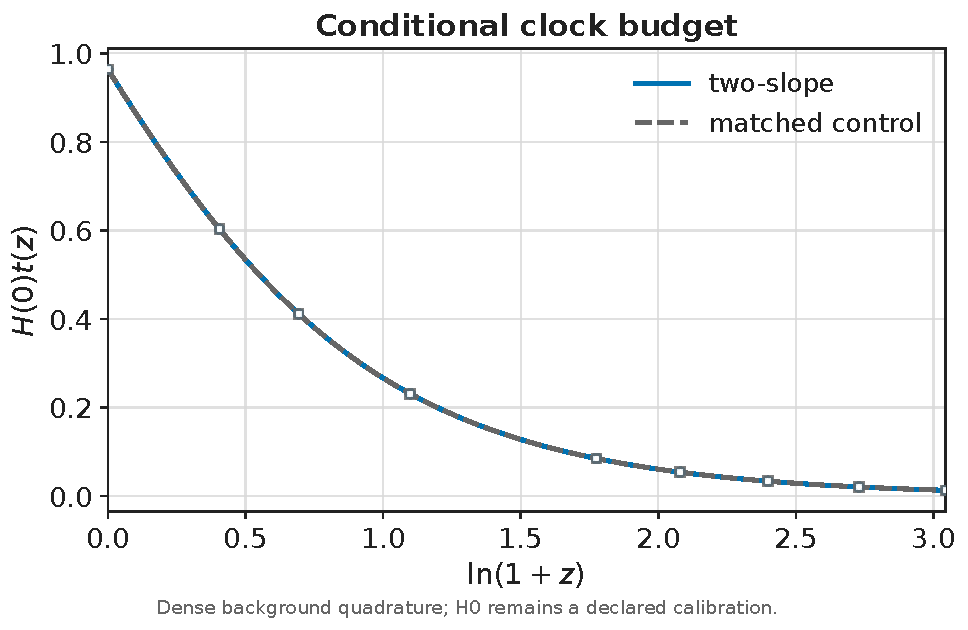
\includegraphics[width=\textwidth,height=0.76\textheight,keepaspectratio]{figures/r154/curve_semantics/nonrotation/fig42_b_clock_budget_dense_r154.pdf}
\caption{Conditional dimensionless clock budget $H(0)t(z)$ for the
supplied two-slope action/state and its same-present-fraction reference
control.  Named expansion, comoving distance, total kinematic $w_{\rm eff}$,
the calibrated family and the explicit scope statement are separate
full-width atlas panels.  The continuous traces are replayed from the frozen 3001-point
background owner, while the nine published redshift nodes are retained as
separate markers.  The dense traces and published nodes are direct outputs of
the declared orbit,
not a unique P1--P6 cosmology or a dark-energy equation-of-state fit.  Colour
is redundant with marker and line style.  \textit{Display semantics: \detokenize{The continuous clock traces are replayed from the frozen 3001-point background owner; the nine published nodes are shown separately.}}}
\label{fig:r103_ect_background_clocks}
\end{figure}
\par\smallskip\noindent The complementary conditional background and scope panels are retained in Appendix~\ref{app:r129_visual_background_cosmology}.
\begin{figure}[p]
\centering
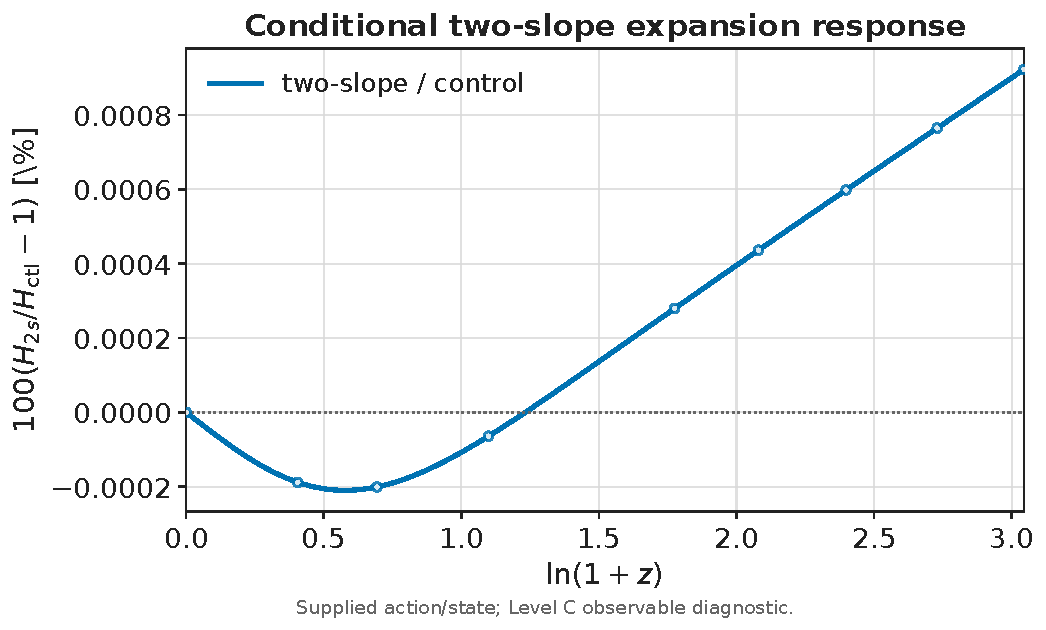
\includegraphics[width=\textwidth,height=0.76\textheight,keepaspectratio]{figures/r154/curve_semantics/nonrotation/fig43_a_two_slope_expansion_dense_r154.pdf}
\caption{Focused status-safe fractional expansion response of the
supplied two-slope background relative to the matched control.  The total
kinematic $w_{\rm eff}=-1-2H'/(3H)$ is a separate full-width atlas panel; the
inverse-$F$ background proxy follows as a continuation and is not a local
Newton constant.  The curves contain no common-$\varepsilon$ law.  They are
Level A only inside the supplied action and state, and a Level-C observable
diagnostic rather than a unique P1--P6 cosmology.  Colour is redundant with line style, marker shape and marker
fill.  The continuous expansion trace is replayed from the frozen 3001-point
background owner; the nine published redshift nodes are retained as separate
markers rather than used as vertices of a polygonal guide.  \textit{Display semantics: \detokenize{The continuous expansion trace is replayed from the frozen 3001-point background owner; the nine published nodes are shown separately.}}}
\label{fig:r103_two_slope_HwG_conditional}
\end{figure}

\begin{figure}[p]
\centering
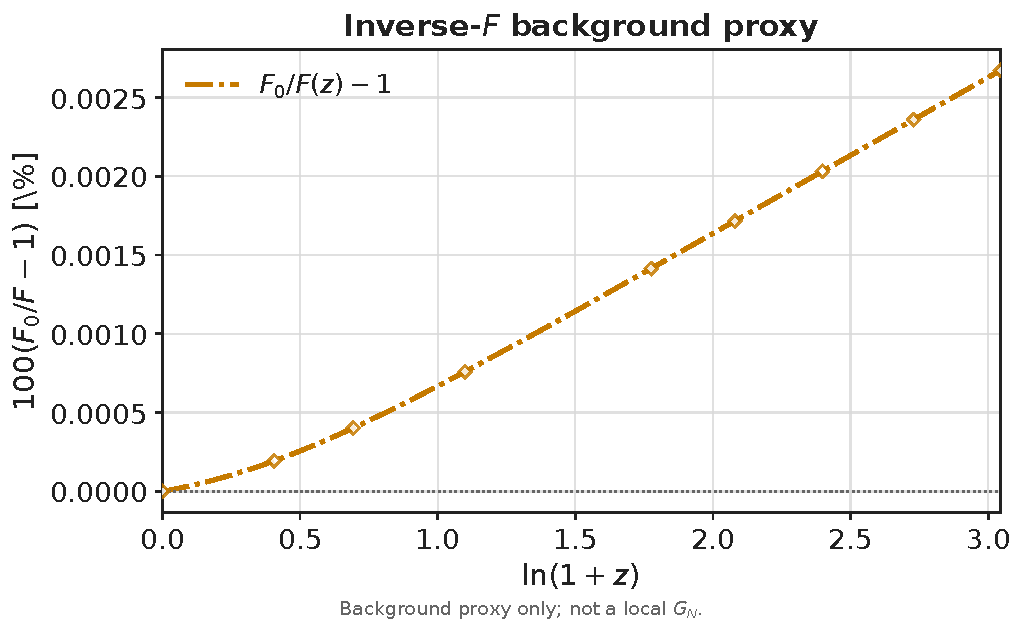
\includegraphics[width=\textwidth,height=0.76\textheight,keepaspectratio]{figures/r154/curve_semantics/nonrotation/r149_inverse_f_proxy_dense_r154.pdf}
\caption*{\textbf{Figure~\ref{fig:r103_two_slope_HwG_conditional}, continued.} Inverse-$F$ background proxy.  It is not a local Newton constant; a finite-body metric and PPN map remain Open.  The intermediate $w$ panel is retained in the visual atlas.  \textit{Display semantics: \detokenize{The continuous inverse-F trace is evaluated directly on the frozen 3001-point background owner; the nine published nodes are shown separately.}}}
\end{figure}
The corresponding distance differences from the control stay below
$1.5\times10^{-4}\%$ on $0<z\le20$.  Thus this particular near-GR state is
a constructive viable-background benchmark, not a mechanism for a large
late-distance shift.

\paragraph{Conditional high-redshift time budgets.}
At the externally supplied rounded reference calibration
$H_0=67.4$ km\,s$^{-1}$\,Mpc$^{-1}$, corresponding to the named Planck
base-$\Lambda$CDM inference $67.36\pm0.54$
km\,s$^{-1}$\,Mpc$^{-1}$~\cite{Planck2018}, the same ECT-candidate orbit
gives
\begin{equation}
 \begin{array}{c|ccccc}
 z&4.9&7&10&14.32&20\\ \hline
 t_{2s}(z)\ [{\rm Gyr}]&1.22645&0.77690&0.48143&0.29241&0.18177
 \end{array}
 \label{eq:two_slope_high_z_ages}
\end{equation}
and the intervals $(z_{\rm form}\!\to z_{\rm obs})=(10\to4.9)$,
$(14.32\to7)$, $(20\to10)$ and $(20\to14.32)$ are respectively
$0.74502$, $0.48450$, $0.29966$ and $0.11064$~Gyr.  With
$H_0=73.04$ the corresponding intervals are $0.68750$, $0.44709$,
$0.27652$ and $0.10210$~Gyr.  These are genuine clock outputs of the supplied
two-slope dynamics after dimensional matching.  They are not a JWST
abundance prediction: stellar-population inference, primordial power,
scale-dependent growth, halo collapse, baryonic assembly and survey
selection still have to be propagated through the same completion.

\paragraph{Conditional quasistatic growth diagnostic.}
As a deliberately restricted first perturbative estimate, impose conserved
pressureless Jordan matter, a subhorizon quasistatic limit, negligible scalar
mass and mixing, scale-independent response and
$\mu_{\rm QS}=F_s(0)/F_s(N)$.  Then
\begin{equation}
 D''+\left(2+{H'\over H}\right)D'
 -{3\over2}{\rho_m\over3F_s(0)H^2}\mu_{\rm QS}D=0.
 \label{eq:two_slope_growth_diagnostic}
\end{equation}
Normalising $D(0)=1$, the fractional difference from the matched control is
\begin{equation}
\begin{array}{c|rrrr}
z&0.5&1&2&4.9\\ \hline
10^4\Delta D/D_{\rm ctl}\ [\%]&-1.04&-2.51&-5.17&-9.95\\[2pt]
z&7&10&14.32&20\\ \hline
10^4\Delta D/D_{\rm ctl}\ [\%]&-12.09&-14.31&-16.60&-18.74
\end{array}
\end{equation}
This near-GR result is numerically small.  Its status is Level~C conditional
because the complete gauge-reduced
scalar/vector/tensor action, physical metric, scalar mass, scale dependence,
initial spectrum, non-linear evolution and bias likelihood have not been
derived.

\paragraph{Owner-specific early-response envelope (separate from the
two-slope orbit).}
The following calculation is not another trajectory of the named two-slope
action and does not restore a universal common-$\varepsilon$ cosmology.  It is
a deliberately restricted response-envelope calculation in which a constant
channel slope $\zeta_{\rm ER}$ dresses the matter and constant-source terms,
but not radiation:
\begin{align}
 E_{\rm ER}^{\,2}(N)
 &=\Omega_r e^{-4N}
   +\Omega_m e^{-(3+2\zeta_{\rm ER})N}
   +\Omega_\Lambda e^{-2\zeta_{\rm ER}N},
 \label{eq:ect_zetaER_scenario_background}\\
 \Omega_m^{\rm grav}(N)
 &=\frac{\Omega_m e^{-(3+2\zeta_{\rm ER})N}}
 {E_{\rm ER}^{\,2}(N)},
 \qquad
 \mu_{\rm ER}(N)=e^{-2\zeta_{\rm ER}N}.
 \label{eq:ect_zetaER_scenario_matter}
\end{align}
The factor $\mu_{\rm ER}$ already appears once in
$\Omega_m^{\rm grav}$.  The single-count restricted growth equation is
therefore
\begin{equation}
 D_{NN}+\left(2+\frac{E_{{\rm ER},N}}{E_{\rm ER}}\right)D_N
 -\frac32\Omega_m^{\rm grav}D=0,
 \label{eq:ect_zetaER_growth_single_count}
\end{equation}
without a second factor of $\mu_{\rm ER}$ in the source.  This closure differs from
the near-GR two-slope calculation in
Eq.~\eqref{eq:two_slope_growth_diagnostic}; their outputs must not be merged
or described as one action/state prediction.

\paragraph{Initial-mode and boundary semantics.}
Write $N_{\rm on}=-\ln(1+z_{\rm on})$ and
$B_{\rm on}=2+(E_{{\rm ER},N}/E_{\rm ER})_{N_{\rm on}}$.
The common-normalisation boundary is fixed by
\begin{equation}
 D(N_{\rm on})=a_{\rm on}=e^{N_{\rm on}},
 \qquad
 D_N(N_{\rm on})=p_0D(N_{\rm on}),
 \qquad
 p_0=\frac{-B_{\rm on}+
 \sqrt{B_{\rm on}^{\,2}+6\Omega_m^{\rm grav}(N_{\rm on})}}{2}.
 \label{eq:ect_zetaER_initial_mode}
\end{equation}
The first condition fixes the source calculation's scale-factor
normalisation; equivalently, the rescaled variable $D/a_{\rm on}$ has unit
value at the boundary.  The second condition selects the local growing
eigenmode.  In this sensitivity calculation
$z_{\rm on}$ is the boundary at which the model and control are assigned the
same primordial normalisation.  It is not a derived activation redshift, a
phase-transition epoch, or a switch in the action.

\paragraph{Exact equality identity inside the same envelope.}
With only the matter term in
Eq.~\eqref{eq:ect_zetaER_scenario_background} tilted relative to radiation,
matter--radiation equality obeys
\begin{equation}
 1+z_{\rm eq}(\zeta_{\rm ER})
 =\left(\frac{\Omega_m}{\Omega_r}\right)^{1/(1-2\zeta_{\rm ER})},
 \qquad
 \frac{1+z_{\rm eq}(\zeta_{\rm ER})}{1+z_{\rm eq}(0)}
 =\left(\frac{\Omega_m}{\Omega_r}\right)^{
 2\zeta_{\rm ER}/(1-2\zeta_{\rm ER})}.
 \label{eq:ect_zetaER_equality_identity}
\end{equation}
This is an exact identity of the declared envelope, not a CMB or BAO
prediction.  A radiation tilt, an independently derived transfer sector, or
a different physical metric changes the interpretation and can be
degenerate with it.

\paragraph{Numerical growth and collapse sensitivity.}
For $z_{\rm on}=1000$, $z=10$, $\Omega_m=0.315$ and
$\Omega_r=9.2\times10^{-5}$, flat closure fixes
$\Omega_\Lambda=1-\Omega_m-\Omega_r=0.684908$.  Independent solvers
reproduce the following single-count results.  The five $\zeta_{\rm ER}$
values are frozen
stress-test coordinates inherited from the audited calculation chain; they
are not posterior samples, an allowed corridor, or predictions of ECT.  The
exact inputs underlying the first three displayed rows are
$1.5612556036955692\times10^{-6}$,
$0.007500442556492628$ and $0.029588344765651916$; the first table column is
rounded only for layout.  The conditional barrier is obtained from a pressureless
spherical top-hat in the same envelope,
\begin{equation}
 \delta_{NN}+\left(2+\frac{E_{{\rm ER},N}}{E_{\rm ER}}\right)\delta_N
 -\frac{4}{3}\frac{\delta_N^2}{1+\delta}
 -\frac32\Omega_m^{\rm grav}\delta(1+\delta)=0,
 \label{eq:ect_zetaER_tophat_sensitivity}
\end{equation}
with the same growing-mode initial slope and a frozen numerical collapse
criterion $\delta=10^7$.  The reported barrier is the corresponding linear
solution extrapolated to the observation slice; the control value is
$\delta_{c,0}=1.7267600460$.  For an external reference peak height $\nu=5$,
the fixed-barrier and top-hat cumulative sensitivities are
\begin{align}
 R_{\rm PS}^{\rm fixed}
 &=\frac{\operatorname{erfc}\!\left[
 \nu/(\sqrt2 D/D_0)\right]}
 {\operatorname{erfc}(\nu/\sqrt2)},
 \label{eq:ect_zetaER_cumulative_ps_fixed_sensitivity}\\
 R_{\rm PS}^{\rm top\mbox{-}hat}
 &=\frac{\operatorname{erfc}\!\left[
 \nu(\delta_c/\delta_{c,0})/(\sqrt2 D/D_0)\right]}
 {\operatorname{erfc}(\nu/\sqrt2)}.
 \label{eq:ect_zetaER_cumulative_ps_sensitivity}
\end{align}
\begingroup
\small
\setlength{\tabcolsep}{3.2pt}
\setlength{\LTpre}{4pt}
\setlength{\LTpost}{4pt}
\renewcommand{\arraystretch}{0.92}
\begingroup
\setlength{\LTleft}{0pt}
\setlength{\LTright}{0pt}
\setlength{\tabcolsep}{1pt}
\begin{longtable}{@{\extracolsep{\fill}}r r r r r r r@{}}
\caption{Owner-specific $\zeta_{\rm ER}$ sensitivity envelope.  None of the
rows is the named two-slope orbit or a joint JWST/CMB likelihood.}
\label{tab:ect_zetaER_growth_collapse_sensitivity}\\
\toprule
$\zeta_{\rm ER}$ & $D/D_0$ &
$(1+z_{\rm eq})/(1+z_{\rm eq,0})$ &
$\delta_c$ & $\delta_c/\delta_{c,0}$ &
$R_{\rm PS}^{\rm fixed}$ & $R_{\rm PS}^{\rm top\mbox{-}hat}$\\
\midrule
\endfirsthead
\toprule
$\zeta_{\rm ER}$ & $D/D_0$ &
$(1+z_{\rm eq})/(1+z_{\rm eq,0})$ &
$\delta_c$ & $\delta_c/\delta_{c,0}$ &
$R_{\rm PS}^{\rm fixed}$ & $R_{\rm PS}^{\rm top\mbox{-}hat}$\\
\midrule
\endhead
\bottomrule
\endfoot
$1.5612556\times10^{-6}$ & 1.00000521 & 1.00002541 & 1.72676032 & 1.00000016 & 1.00013505 & 1.00013091\\
0.00750044 & 1.02494986 & 1.13195313 & 1.72810966 & 1.00078159 & 1.86656763 & 1.83082689\\
0.02958834 & 1.09767905 & 1.66846599 & 1.73234129 & 1.00323220 & 9.13465297 & 8.51585875\\
0.03300000 & 1.10882221 & 1.77730862 & 1.73302549 & 1.00362844 & 11.34568870 & 10.50228040\\
0.03755500 & 1.12366682 & 1.93658864 & 1.73395051 & 1.00416414 & 14.99787480 & 13.75594876\\
\end{longtable}
\endgroup
\endgroup

\begin{figure}[p]
\centering
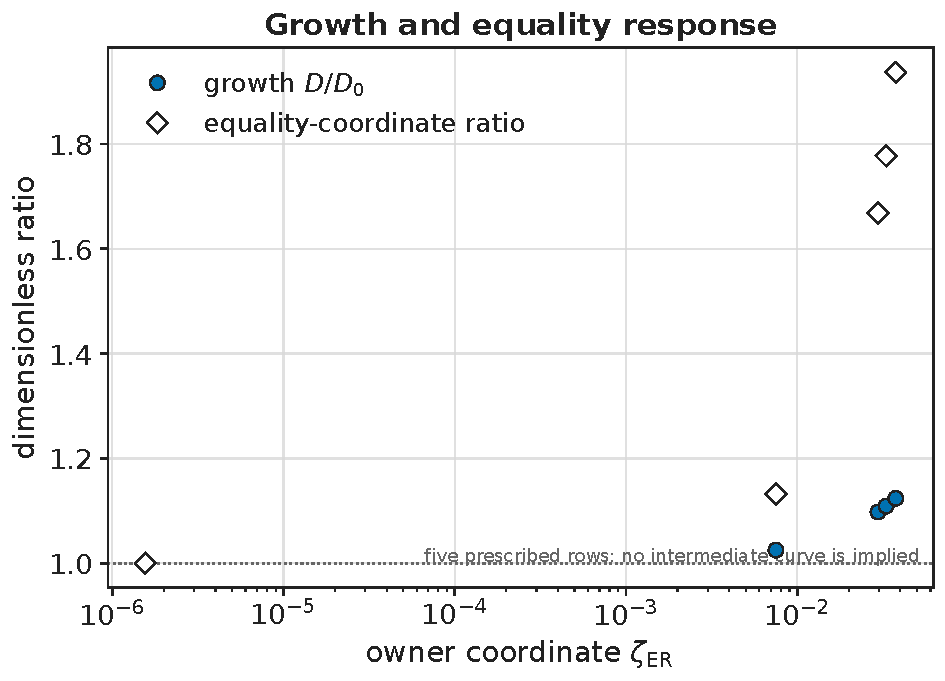
\includegraphics[width=\textwidth,height=0.76\textheight,keepaspectratio]{figures/r154/curve_semantics/nonrotation/fig44_a_growth_equality_nodes_r154.pdf}
\caption{Owner-specific early-response sensitivity envelope at $z=10$ for
the five prescribed $\zeta_{\rm ER}$ stress-test coordinates of
Table~\ref{tab:ect_zetaER_growth_collapse_sensitivity}.  Linear growth and
the equality shift are algebra inside the declared envelope; the top-hat
barrier and Press--Schechter rare-tail ratios are Level-C sensitivity
estimates.  The five prescribed source rows are rendered as
unconnected markers; no interpolant, continuous family, posterior, JWST
abundance prediction or likelihood is inferred.  Colour is redundant with marker shape, marker fill and direct legend text, so the panel remains
interpretable in grayscale.  The remaining owner panel follows as a full-width continuation.  \textit{Display semantics: \detokenize{The five prescribed owner rows are shown as unconnected markers; no intermediate interpolation is implied.}}}
\label{fig:r114_early_response_growth_collapse_envelope}
\end{figure}

\begin{figure}[p]
\centering
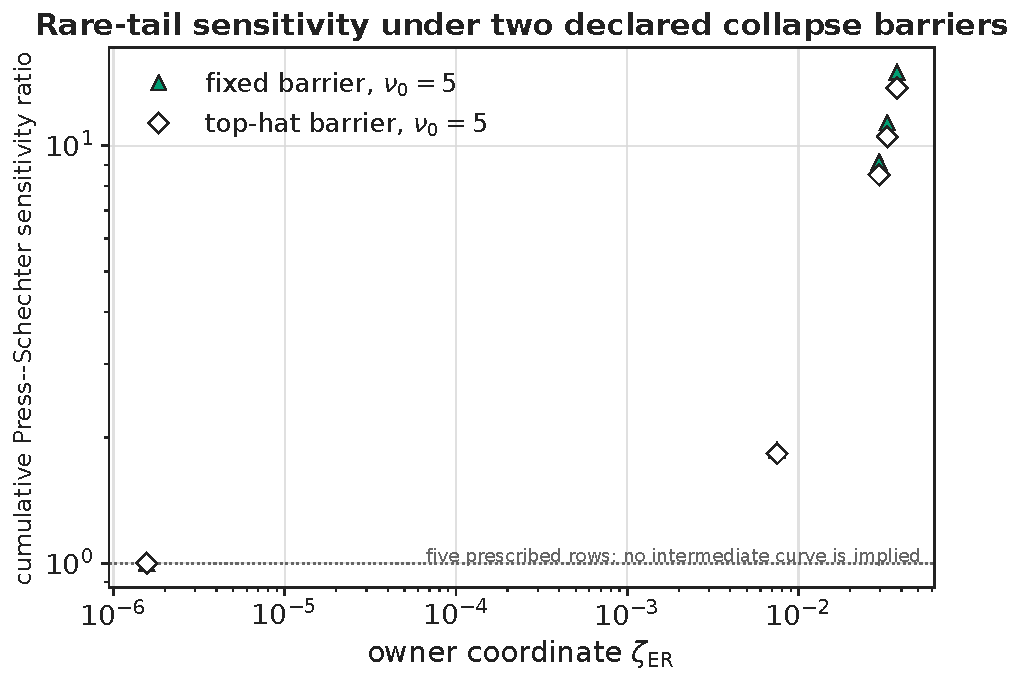
\includegraphics[width=\textwidth,height=0.76\textheight,keepaspectratio]{figures/r154/curve_semantics/nonrotation/r149_rare_tail_nodes_r154.pdf}
\caption*{\textbf{Figure~\ref{fig:r114_early_response_growth_collapse_envelope}, continued.} Conditional top-hat and Press--Schechter rare-tail sensitivity.  The same five discrete stress-test rows are unconnected markers and do not define a continuous response family.  This is Level C and is not a JWST abundance prediction or likelihood.  \textit{Display semantics: \detokenize{The five prescribed rare-tail rows are shown as unconnected markers; no intermediate interpolation is implied.}}}
\end{figure}

The first numerical column is Level~A inside
Eqs.~\eqref{eq:ect_zetaER_scenario_background}--
\eqref{eq:ect_zetaER_initial_mode}; the equality column is exact algebra in
that envelope.  The top-hat barrier and Press--Schechter ratios are Level~C
sensitivity estimates.  They omit a derived ECT primordial spectrum,
scale-dependent transfer, baryons, calibrated halo multiplicity, mass
inference and selection.  They therefore show that an early response can
produce a large rare-tail sensitivity while simultaneously shifting equality;
they do not constitute a JWST abundance prediction or re-establish a common
$\varepsilon$ theory.  In particular, no displayed row has yet closed
equality, early growth or JWST abundance, transfer physics and Solar-System
constraints in one action/state solution: the near-zero row produces
negligible rare-tail enhancement, whereas the boosted rows shift the declared
equality coordinate by approximately $13$--$94\%$.  This is a cross-sector
tension to be resolved by a derived radiation/transfer and metric completion,
not evidence that any one row is observationally viable.

\paragraph{Conditional sound-horizon diagnostic.}
If one additionally imports a standard photon/recombination layer with
$\Omega_b=0.0493$, $\Omega_\gamma=5.45\times10^{-5}$,
$z_{\rm drag}=1059.94$, $c_\gamma=c$ and
$c_s/c=[3(1+3\rho_b/4\rho_\gamma)]^{-1/2}$, the same orbit gives
\begin{equation}
 {H(0)r_s\over c}=0.03272615,\qquad
 {\Delta r_s\over r_{s,\rm ctl}}=-0.003157\%.
 \label{eq:two_slope_conditional_sound_horizon}
\end{equation}
This equals $145.565$~Mpc for the $67.4$ calibration and $134.324$~Mpc for
the $73.04$ calibration.  Recombination and the dimensional normalisation are
external inputs here, so these numbers neither infer $H_0$ nor resolve its
early/late discrepancy.  They instead show quantitatively that the frozen
near-GR member leaves the control sound horizon essentially unchanged.

\paragraph{Numerical validation and immediate falsifiers.}
The background was integrated independently with DOP853 and Radau at
relative tolerance $10^{-11}$; $\tau_{2s}$ agrees below $5\times10^{-13}$.
On 3001 points, $F_s$, $H^2$, the algebraic Friedmann denominator and
$\Delta_{Hv}$ remain positive.  The present dimensionless Planck drift is
$d\ln F_s/dN=3.1225\times10^{-6}$ for this frozen state.  A publication
claim still requires a finite-body PPN solution, a direct comparison of the
dimensional drift with local bounds, and the full perturbation/recombination
owners just listed.

\paragraph{Calibrated family scan and the early-time/drift trade-off.}
To test whether the preceding near-GR point hides a useful high-redshift
effect, a second frozen scan used $c_s=a_s$, $b_s=3a_s$ and imposed the vacuum
root $\sigma_{\rm vac}=0$ by
\begin{equation}
 {V_-\over V_+}={b_s-2a_s\over2a_s-c_s}=1.
 \label{eq:two_slope_scan_vacuum_ratio}
\end{equation}
For each $(a_s,\kappa_s)$, the early frozen value and total potential
normalisation were shot to $\sigma(0)=0$, $H(0)=1$, with
$\Omega_{m0}=0.315$ and $\Omega_{r0}=9.19\times10^{-5}$.  DOP853 and Radau
agree in $\tau_{2s}$ better than $10^{-15}$ for all nine points, and every
sampled $F_s$, Friedmann denominator and response determinant is positive.
\begingroup
\setlength{\LTleft}{0pt}
\setlength{\LTright}{0pt}
\begin{longtable}{@{\extracolsep{\fill}}r r r r r r@{}}
\caption{Technical solver replay of the calibrated two-slope scan.  This
table records background age, early-clock, local-limit and drift diagnostics;
the main cross-channel result including sound horizon, early coupling and the
rough acoustic rescaling is
Table~\ref{tab:two_slope_calibrated_scan_expanded}.  The comparison is the flat
radiation--matter--constant-source control with the same present density
fractions.  The fifth column is the exact unscreened massless scalar limit;
the last is the homogeneous-background quantity
$|d\ln G_{{\rm div},s}/dN|_0=|d\ln F_s^{-1}/dN|_0$.  Neither that divided
coefficient nor the fifth-column unscreened proxy substitutes for a screened
finite-body solution.}
\label{tab:two_slope_calibrated_scan}\\[-6pt]
\toprule
$a_s$ & $\kappa_s$ & $\Delta t_0$ [\%] &
$\Delta t(z{=}10)$ [\%] & $|\gamma_{\rm PPN}-1|_{\rm uns}$ &
$|d\ln G_{{\rm div},s}/dN|_0$ \\
\midrule
\endfirsthead
\bottomrule
\endfoot
0.01&0.05&+0.00332&$-0.1930$&$1.99\times10^{-3}$&$8.96\times10^{-4}$\\
0.03&0.05&+0.02926&$-1.6994$&$1.74\times10^{-2}$&$7.90\times10^{-3}$\\
0.08&0.05&+0.18126&$-10.4912$&$1.02\times10^{-1}$&$4.93\times10^{-2}$\\
0.01&1&+0.00017&$-0.0097$&$1.00\times10^{-4}$&$4.49\times10^{-5}$\\
0.03&1&+0.00150&$-0.0870$&$8.98\times10^{-4}$&$4.04\times10^{-4}$\\
0.08&1&+0.01056&$-0.6140$&$6.32\times10^{-3}$&$2.85\times10^{-3}$\\
0.01&10&+0.00002&$-0.0010$&$1.00\times10^{-5}$&$4.49\times10^{-6}$\\
0.03&10&+0.00015&$-0.0087$&$9.00\times10^{-5}$&$4.04\times10^{-5}$\\
0.08&10&+0.00106&$-0.0619$&$6.39\times10^{-4}$&$2.87\times10^{-4}$\\
\end{longtable}
\endgroup
Indeed, with $\Phi_{\rm BD}=F_s$ the action has constant
$\omega_{\rm BD}=\kappa_s/a_s^2$, so in the unscreened light-scalar limit
\begin{equation}
 \gamma_{\rm PPN}={\omega_{\rm BD}+1\over\omega_{\rm BD}+2}
 ={\kappa_s+a_s^2\over\kappa_s+2a_s^2},\qquad
 \beta_{\rm PPN}=1.
 \label{eq:two_slope_unscreened_ppn}
\end{equation}
The corresponding weak-body coupling and Cavendish coefficient are given by
Eq.~\eqref{eq:two_slope_Gcav_transfer}; they are distinct from
$G_{{\rm div},s}$ before that response limit is imposed.
Under the same explicitly imported standard photon/recombination inputs used
in Eq.~\eqref{eq:two_slope_conditional_sound_horizon}, the scan gives
\begin{equation}
 {\Delta r_s\over r_{s,\rm ctl}}[\%]=
 \begin{array}{c|ccc}
  &a_s=0.01&a_s=0.03&a_s=0.08\\ \hline
 \kappa_s=0.05&-0.642&-5.546&-30.646\\
 \kappa_s=1&-0.0323&-0.290&-2.031\\
 \kappa_s=10&-0.00323&-0.0290&-0.206
 \end{array}.
 \label{eq:two_slope_scan_sound_horizon}
\end{equation}
This is sound-horizon leverage, not an inferred $H_0$: the distance to last
scattering, recombination perturbations and late likelihood have not been
fitted.  The deliberately crude fixed-acoustic-angle proxy
$H_{0,\theta}^{\rm proxy}=67.4\,r_{s,\rm ctl}/r_s$ gives
$H_{0,\theta}^{\rm proxy}=(67.84,71.36,97.18)$
km\,s$^{-1}$\,Mpc$^{-1}$ along the three $\kappa_s=0.05$ rows, and
$(67.60,68.80)$ for $(a_s,\kappa_s)=(0.03,1),(0.08,1)$.  These numbers expose
the possible acoustic leverage only; they are not a CMB or distance-ladder
likelihood.  The row $(a_s,\kappa_s)=(0.03,0.05)$ illustrates the central
trade-off: it changes $r_s$ by $-5.55\%$ but has the unscreened
$|\gamma_{\rm PPN}-1|=0.0174$.  The only scanned row satisfying the displayed
absolute $\gamma$ proxy gate without screening, $(0.01,10)$, changes $r_s$ by merely
$-0.00323\%$.  The corresponding early-to-present divided-coefficient ratios
$G_{{\rm div},s}^{\rm early}/G_{{\rm div},s}^{0}
=F_s(0)/F_{s,\rm early}$ are $1.1411$ and $1.000075$, respectively (the
strongest scanned $-30.65\%$ sound-horizon row reaches $2.3255$).  Any large
acoustic effect is therefore correlated with divided Planck-coefficient
drift, but its physical gravitational calibration and BBN viability are
determined only by the complete early-universe response pipeline.

The scan establishes a concrete negative result for the nine evaluated nodes:
the points that most change the early time budget make the Universe
\emph{younger} at fixed high redshift and simultaneously increase the
homogeneous divided Planck-coefficient drift.  The last column is
$|d\ln G_{{\rm div},s}/dN|_0$ and cannot be compared directly with lunar
ranging~\cite{Uzan2011,Williams2004}; LLR constrains an orbital/Cavendish
response after the scalar range and body charges are specified.  The primary
Cassini result $\gamma_{\rm PPN}-1=(2.1\pm2.3)\times10^{-5}$
\cite{Bertotti2003} is compared here only with the explicitly unscreened
massless-scalar proxy.  In that limit one of the nine nodes,
$(a_s,\kappa_s)=(0.01,10)$, passes the displayed absolute $\gamma$ gate; it is
$1.35\sigma$ from the measured central value and changes $t(z=10)$ by only
$-9.7\times10^{-4}\%$.  Each sampled node with a large early-time effect
therefore requires a separately derived finite-body or metric completion.
The finite-body mechanism analysed for the named calibration supplies no mass
screening, but neither that result nor failure to find another completion
rejects unsampled members of the continuous two-parameter family.  The
current result is a reproducible nine-node action/state scan, not a fitted
effective one-parameter law or an exhaustive family no-go.

The exact radiation limit, exact dust tracker, stable vacuum and global
two-solver orbit establish a Level~A existence result inside the supplied
action and a Level~B proof-of-class for an ECT completion.  They do
\emph{not} select a unique physical $H_{\rm ECT}(a)$ or
$t_{0,\rm ECT}$ from P1--P6.  They do identify the conditional curves and
clock outputs of the explicitly supplied completion above.  The next gates are:
derive Eq.~\eqref{eq:two_slope_action} and its parameters from the ordered
$\Phi$-medium; identify the physical matter/photon metric and ordering event;
derive the gauge-reduced perturbation action; and pass BBN, recombination,
varying-$G$, growth, lensing and finite-body PPN tests.  No spherical boundary
or spherical Universe is assumed in this construction.

\subsection{Relation to observables}

The two-slope example demonstrates the distinction between an action-owned
conditional observable and a unique ECT prediction.  Its background clocks
and distances are computed directly; its growth and sound horizon require
the disclosed extra assumptions.  For any future completion, recombination
and photon propagation precede
the Hubble likelihood; the quadratic perturbation action precedes growth,
ISW and lensing; a non-linear halo and baryonic forward model precedes JWST.
The complete owner matrix and acceptance gates are given in
\S\ref{sec:ect_cosmology_closure} and
Appendix~\ref{app:ect_cosmology_identifiability}.

\section{Conditional tensor-EFT scaffold for gravitational waves associated
with ordering}
\label{app:ordering_gw_scaffold}
% ==============================================================

This appendix provides a minimal dimensional scaffold for a possible
stochastic gravitational-wave background associated with inhomogeneous
ordering.  It applies only after a physical Lorentzian tensor EFT, a
clock/metric, a TT source vertex and a matching interface from ordering
inhomogeneities to that tensor have been supplied.  It therefore
parametrises a late-stage or post-ordering transfer; it is not a
first-principles calculation of the pre-Lorentzian ordering process and does
not assert that ordering produces a nonzero tensor source.  Its purpose is to
make the conditional programme of \S\ref{sec:ordering_gw} quantitatively
traceable without promoting it to a prediction.

\paragraph{Source equation.}
For the constant-$(M_T,c_T)$ tensor benchmark on an emergent FRW background,
define the dimensionless physical transverse--traceless metric perturbation by
$g_{ij}=a^2(\delta_{ij}+H_{ij})$, with
$\partial_iH_{ij}=H_{ii}=0$.  In conformal time $\eta$ and units $c=1$ it
satisfies
\begin{equation}
  H''_{ij}+2\mathcal{H}H'_{ij}+c_T^2k^2 H_{ij}
  =\frac{2a^2}{M_T^2}\Pi^{{\rm TT},{\rm phys}}_{ij}
  \equiv\frac{2}{M_T^2}\Pi^{{\rm TT},{\rm conf}}_{ij},
  \qquad
  \Pi^{{\rm TT},{\rm conf}}_{ij}:=
  a^2\Pi^{{\rm TT},{\rm phys}}_{ij},
  \label{eq:gw_source_app}
\end{equation}
where $\Pi^{{\rm TT},{\rm phys}}_{ij}$ is the TT projection of the physical
orthonormal spatial anisotropic stress (equivalently the mixed spatial stress
on this background, with displayed spatial indices moved by $\delta_{ij}$),
and the second symbol is its explicitly defined conformal rescaling.  Only in
the GR-normalised specialization
$c_T=1$ and $M_T^2=(8\pi G_N^{\rm nat})^{-1}$ does the right-hand side become
$16\pi G_N^{\rm nat}a^2\Pi^{{\rm TT},{\rm phys}}_{ij}
=16\pi G_N^{\rm nat}\Pi^{{\rm TT},{\rm conf}}_{ij}$.  A time-dependent
$M_T$ changes the damping term and lies outside this minimal benchmark.
Specifically, allowing $M_T=M_T(\eta)$ in the same reduced action replaces
$2\mathcal H$ by $2\mathcal H+(M_T^2)'/M_T^2$.  Neither the TT stress nor its
coupling is supplied by P1--P6.

\paragraph{Dimensional estimate.}
Up to convention-dependent order-one factors, the characteristic tensor
amplitude at production scales in natural units as
\begin{equation}
  H_{\rm prod}\sim
  \frac{2\,\Delta\rho\,L_{\rm corr}^2}{M_T^2c_T^2}
  \quad\longrightarrow\quad
  \frac{16\pi G_N^{\rm SI}\,\Delta\rho\,L_{\rm corr}^2}{c^4}
  \quad\text{in the GR-normalised SI benchmark},
  \label{eq:h_prod_estimate}
\end{equation}
where $\Delta\rho$ is a physical TT stress/energy-density scale, not the
full ordering energy density unless its TT projection is derived, and
$L_{\rm corr}$ is the gradient-controlled correlation length of the matched
source.  The displayed coefficient follows from the chosen tensor-action
normalisation; source geometry, TT projection and time-profile factors remain
parametric.
The peak frequency at production is parametrically set by
\begin{equation}
  f_{\rm prod}\sim \frac{c_T}{2\pi L_{\rm corr}}\quad(c=1)
  \quad\longrightarrow\quad \frac{c}{2\pi L_{\rm corr}}
  \quad\text{in the GR-normalised SI benchmark}.
  \label{eq:f_prod_estimate}
\end{equation}

\paragraph{Redshift to today.}
If the ordering transition occurs at an effective redshift
$z_{\rm ord}$, the peak frequency today is approximately
\begin{equation}
  f_0 \sim \frac{f_{\rm prod}}{1+z_{\rm ord}},
  \label{eq:f_today}
\end{equation}
while the present-day gravitational-wave energy fraction is related to
its production value by the standard redshifting logic
\begin{equation}
  \Omega_{{\rm GW},0}(f_0)
  \sim
  \Omega_{{\rm GW},{\rm prod}}(f_{\rm prod})
  \left(\frac{a_{\rm ord}}{a_0}\right)^4
  \left(\frac{H_{\rm ord}}{H_0}\right)^2.
  \label{eq:OmegaGW_scaffold}
\end{equation}
Thus the present signal depends not only on the source strength at
production but also on the subsequent expansion history.

\paragraph{What this does and does not provide.}
Equations~\eqref{eq:h_prod_estimate}--\eqref{eq:OmegaGW_scaffold}
provide a dimensional scaffold, not a closed prediction.
The quantity $\Omega_{{\rm GW},{\rm prod}}$ must itself be obtained
from the ordering-source efficiency and cannot yet be computed from
first principles within the present closure.
The quantities $\Delta\rho$, $L_{\rm corr}$, and $z_{\rm ord}$ are
transition parameters that must be derived from the ordering dynamics
(duration, latent heat analogue, correlation length, domain structure).
Until this microphysics is closed, $\Omega_{\rm GW}(f)$ remains
parametrically open.

\paragraph{Distinction from standard first-order transitions.}
The ECT ordering transition is not a thermal bubble-nucleation event
in a pre-existing Lorentzian spacetime.
Standard thermal-transition formulae (e.g.\ based on $\alpha$,
$\beta/H$, $v_w$) therefore cannot be applied directly.
The scaffold above is formulated in terms of general dimensional
quantities applicable to any causal source of anisotropic stress,
without assuming a thermal equation of state.

% ==============================================================

\section{Status of sign-level ordered-branch cosmology statements}
\label{app:cosmo_sign_theorems}

This appendix separates exact statements inside a supplied scalar model from
claims that require a cosmological completion.

\paragraph{C1.~Conditional bare scalar-ratio inequality.}
For the action normalisation of Eq.~\eqref{eq:phi_first_action},
$K_\phi^{\rm phys}=\bar M_{\rm Pl}^2\omega\dot\phi^2/2\ge0$ and
$K_\phi^{\rm phys}+U>0$ imply
$w_\phi^{\rm bare}=(K_\phi^{\rm phys}-U)/
(K_\phi^{\rm phys}+U)\ge-1$.  This is Level~A algebra for the bare
Jordan-bookkeeping pieces.  It is not a bound on the observable effective
history, which also contains $\dot F$ and $\ddot F$.

\paragraph{C2.~Conditional frozen-scalar limit.}
If $\phi$ is constant, the orientation stress vanishes or is separately
fixed, and the remaining potential is constant, the supplied background
equations reduce algebraically to an Einstein--Friedmann form.  Reachability
and stability of that branch are separate questions.

\paragraph{C3.~No model-independent Hubble-shift sign theorem.}
A change in an effective gravitational response can alter both the sound
horizon and distance kernels.  The inferred $H_0$ shift depends on the full
recombination-to-late-time likelihood and is not fixed by the sign of a single
late-time function.  A sign claim is therefore Open until the complete ECT
background, photon metric and acoustic calibration are solved jointly.

\paragraph{C4.~No model-independent JWST enhancement theorem.}
Early-galaxy counts depend on the background volume and age, the primordial
spectrum, transfer and growth, non-linear collapse, baryonic evolution and
selection.  A stronger fitted response in one diagnostic equation is not a
theorem about abundance or morphology.

\paragraph{C5.~Conditional correlation only after common ownership.}
Age, distance, growth and potential evolution are correlated once one
complete action and state determine them.  Their common dependence on an
assumed background does not demonstrate that ECT has derived that background.


\section{ECT cosmological identifiability and action-to-observable closure}
\label{app:ect_cosmology_identifiability}

This appendix gives the equations and gates required for a genuine ECT
cosmology.  Each observable is derived from its physical owner in one common
action and state.

\subsection{Conditional-estimate and replacement policy}

Approximation is not itself a reason to discard a calculation.  A numerical
estimate is admissible as a Level~C conditional result when it is generated by
one named action or response closure, one admissible state and boundary-data
record, one consistent dimensional calibration, and a stated approximation
domain.  The same owners and calibration must then be propagated to every
correlated clock, distance, growth, lensing and local-gravity output.  Universal
postulates need not select the integration constants or the absolute age and
Hubble scale of our particular condensate realisation; those may be measured
state descriptors.  What the theory must determine is the lawful relation
between them for the selected solution.

A formula is rejected only when its algebra is false, its dimensions
or normalisations are inconsistent, or it assigns one unowned parameter to
physically inequivalent operators.  Retirement of that formula does not retire
the physical question.  Each affected observable is retained and replaced by
one of three explicit objects: a conditional calculation from a named
action/state, a theorem or no-go result that bounds the answer, or a forward
equation with its missing owners listed.  A superseded empirical interpolation
is not kept as an active ``legacy'' law in the theory exposition, and an empty
deletion is not an acceptable correction.

\subsection{Frozen action hierarchy}

The bare microscopic scalar action owns local $O(4)$ dynamics, but its P4
gradient background is off shell.  The ordered Euclidean derivative
expansion owns a useful field inventory, while its coefficients and gravity
matching remain Open.  The scalar-only covariant action owns exact field
equations inside its declared Jordan-frame model, but not the orientation
stress.  The supplied two-slope scalar--tensor action owns the conditional
background and clock calculations reported here, while its coefficients,
state and relation to P1--P6 remain inputs.  These layers must not be merged
into one silently complete action.

\subsection{Background boundary/initial-value problem}

A candidate completion must vary one action to obtain a Hamiltonian
constraint, an evolution equation for each independent condensate degree of
freedom, the orientation constraints and matter/radiation conservation.  In
a homogeneous branch, the solve must determine
\begin{equation}
 \mathcal B_{\rm ECT}
 =\{a(t),H(t),u(t),n_A(t),\rho_m(t),\rho_r(t),\ldots\}
 \label{eq:ect_cosmo_background_bundle}
\end{equation}
from one physical state and one set of boundary/initial data.  The Planck
normalisation and $H_0$ may be matched to observations only when explicitly
identified as matching inputs; they cannot simultaneously be advertised as
predictions.

\subsection{Identifiability theorem}

For the current scalar-only equations, the functions in
Eqs.~\eqref{eq:ect_age_inverse_kinetic} and
\eqref{eq:ect_age_inverse_potential} reconstruct an admissible formal closure
for arbitrary sufficiently smooth $H(t)$ and $F(t)>0$.  Hence one background
cannot be inferred from those equations until the closure functions and state
are independently fixed.  Positivity and stability can reject members of the
family but do not select a unique member without additional dynamics.

\subsection{Physical age}

The only active age statement is Eq.~\eqref{eq:ect_age_ordered_branch}.  Its
lower endpoint is the derived ordering event, not automatically $a=0$.
External reference integrations validate a numerical quadrature but do not
constitute ECT ages.  An accepted calculation must publish the full derived
$H_{\rm ECT}(a)$, the ordering criterion, input ownership and independent
integration checks.

\subsection{Distance and acoustic owners}

For a spatially flat physical photon metric, the formal distance and sound
horizon are
\begin{align}
 \chi(z)&=\int_0^z{c_\gamma(z')\over H_{\rm ECT}(z')}\,dz',\\
 D_A(z)&={\chi(z)\over1+z},\\
 r_s(z_*)&=\int_{z_*}^{\infty}{c_s(z)\over H_{\rm ECT}(z)}\,dz.
\end{align}
ECT must derive $c_\gamma$, $c_s$, $z_*$, ionisation history and the metric
seen by photons.  A late-time change cannot be propagated through these
integrals without the high-redshift solution.

\subsection{Perturbation and growth owners}

Let $\mathbf v_k$ denote the constrained physical perturbations after gauge
and non-dynamical fields are removed.  A complete quadratic action has the
form
\begin{equation}
 S^{(2)}={1\over2}\int d\eta\,d^3k\,
 \left[\mathbf v_k'{}^\dagger\mathbf K\mathbf v_k'
 -\mathbf v_k^\dagger\mathbf\Omega^2\mathbf v_k\right].
 \label{eq:ect_cosmo_quadratic_owner}
\end{equation}
Ghost freedom requires positive kinetic form on the physical subspace;
gradient stability requires the relevant eigenvalues of the principal symbol
to be non-negative.  The same reduction must derive the matter Poisson kernel,
slip, sound speeds and anisotropic stress.  Only its solutions can own a
growth factor, $f\sigma_8$, ISW source or lensing kernel.

\subsection{Early-object forward model}

A JWST prediction is a predicted distribution, not a shifted scalar number.
It requires
\begin{equation}
 {dN\over dz\,d\mathcal O}
 = {dV_{\rm ECT}\over dz}
 \int dM\,{dn_{\rm ECT}\over dM}(M,z)\,
 P(\mathcal O\mid M,z,\mathcal B_{\rm baryon})\,
 \mathcal S(\mathcal O,z),
 \label{eq:ect_jwst_forward_model}
\end{equation}
where the volume, halo mass function, baryonic map and selection function are
all declared.  Age and linear growth alone do not fix this observable.

\subsection{Lensing, clusters and mergers}

Photon lensing depends on the Weyl potential of the physical photon metric.
A strictly increasing local transformation preserves the possibly empty
set-valued argmax of the supplied total projected baryon proxy.  Whenever
maximizers are attained, it cannot by itself displace a total-response
maximizer away from the supplied total-baryon maximizers.  It can inherit a
gas/BCG
separation already encoded in the input, and it says nothing about extrema of
the residual map.  Explaining collision-generated morphology therefore
requires a time-dependent
non-local response, its transport state and a hydrodynamic/collision forward
model.  HRC by itself supplies none of these owners.

\subsection{Local gravity and PPN gate}

The cosmological completion and the weak-field finite-source completion must
be limits of the same theory.  The PPN parameters are read from the physical
metric after solving its constraints.  A scalar propagation cone or a
galactic interpolation does not determine them.  Solar-System constraints
are therefore an early kill gate for proposed completions, not an output that
can be appended after a cosmological fit.

\subsection{External Euclidean geometry}

For a nonspherical interface the response depends on intrinsic momentum and
the full extrinsic-curvature tensor.  The admissible external construction
must specify the actual interface, boundary conditions and state and must
derive its contribution to the on-shell Lorentzian stress tensor.  Flat-front
translation and a codimension-one spherical-radius substitution are excluded
as generic Hubble owners by the isometry and Gauss obstructions stated in
\S\ref{sec:universe_age}.

\subsection{Acceptance matrix}

\begin{longtable}{@{}L{0.16\linewidth}L{0.31\linewidth}L{0.34\linewidth}L{0.11\linewidth}@{}}
\toprule
Output & Full ECT-native acceptance evidence & Named supplied result now &
Two-layer status\\
\midrule
Background $H(a)$ & One derived action, state, physical clock/congruence and
stable solve & Globally regular two-slope trajectories; exact
radiation/dust/vacuum limits & Full owner Open; A in supplied action / C as
ECT completion\\
Age & Same $H(a)$ plus congruence depth/lapse map and one declared unit
calibration & $\tau_{2s}=0.96368678$ and disclosed conditional Gyr/high-$z$
clocks; covariance-calibrated $t_0=13.74\pm0.79$~Gyr & Full map Open; A in
state / C dimensional comparison\\
Hubble inference & ECT recombination, spectra and one early+late likelihood &
Official 15-point BC03 covariance calibration of the named orbit plus a
conditional imported-recombination $r_s$ scan and rough fixed-angle diagnostic
& Full inference Open; C calibration/\allowbreak diagnostic\\
JWST & End-to-end abundance and morphology forward model & Conditional
time/volume budgets at nine prespecified nodes; none enlarges the sampled
$t(z=10)$ age budget, while the continuous family is not exhausted &
Full prediction Open; C finite-grid background diagnostic\\
Growth/\allowbreak ISW/\allowbreak lensing & Gauge-reduced perturbation action and photon/matter
metric map & Restricted quasistatic growth plus instantaneous Weyl and
conformal-derivative carriers computed; no projected spectra & Full owner
Open; C limiting diagnostics\\
Clusters & Retarded/non-local metric response plus collision model & Exact
local-map peak no-go only & Full collision/\allowbreak lensing Open; A
conditional theorem / physical Open\\
PPN & Finite-source metric and Solar-System comparison & Exact unscreened
massless-family $\gamma,\beta$ diagnostic; one point satisfies the displayed
absolute-deviation proxy and lies $1.35\sigma$ from the Cassini central value
& Not a full finite-body/PPN fit; full owner Open\\
\bottomrule
\end{longtable}

The right two columns prevent an Open full-theory owner from erasing a valid
conditional result, and prevent a conditional result from being promoted into
an ECT-native prediction.  No fitted cross-channel interval replaces either
layer.



\section{Protocol for a future observable-complete ECT cosmology}
\label{app:ect_cosmology_observable_protocols}

This section defines the calculation that an ECT completion must perform.
The formulae below
are exact definitions or standard consequences of a supplied physical metric,
background and perturbation state.  They are not numerical ECT predictions
until those owners have been obtained from one varied ordered-medium action.
The purpose of writing the chain explicitly is twofold: no missing operator can
be hidden inside a fitted scalar function, and every future result has a finite
set of reproducibility and falsification gates.

\subsection{Minimal action and state record}

A candidate cosmological completion starts from a covariant action record
\begin{equation}
 \mathfrak R_{\rm act}=
 \{S_{\Phi},S_{n},S_{\rm constr},S_{\rm grav},S_{\rm m},S_{\gamma},
   \mathcal B,\Psi_{\rm state}\},
 \label{eq:ect_cosmo_action_record}
\end{equation}
where $\mathcal B$ denotes all boundary terms and interface conditions.  This
record must identify which variables are independent before variation.  In
particular, a director constrained by $n_An^A=1$ and an amplitude related to a
gradient potential cannot subsequently be varied as independent fields.  The
same reduced variable count must be used in the background, perturbation and
finite-source calculations.

The homogeneous state record is
\begin{equation}
 \mathfrak R_{\rm bg}=
 \{a,a_{\rm ord},u,n_A,\rho_i,s_i;
   \mathcal C_0=0,\mathcal C_I=0;\mathcal I_{\rm ord}\},
 \label{eq:ect_cosmo_state_record}
\end{equation}
where $\mathcal C_0$ is the Hamiltonian constraint, $\mathcal C_I$ are all
additional constraints, and $\mathcal I_{\rm ord}=0$ is the relational event
that starts the Lorentzian clock.  A coordinate choice such as $a(t_0)=1$ is
not an initial condition, and a present-day normalisation is not a derivation
of the state.

\paragraph{Background closure gate.}
For evolved variables $X^A$ the numerical system must be written as
\begin{equation}
 \mathbf M_{AB}(X)\,{dX^B\over dN}=\mathbf F_A(X,N),
 \qquad N\equiv\ln a,
 \label{eq:ect_cosmo_first_order_system}
\end{equation}
after all algebraic constraints have been reduced.  A physical trajectory
requires
\begin{equation}
 \det\mathbf M_{\rm phys}\ne0,
 \quad H^2>0,
 \quad F_{\rm grav}>0,
 \quad \lambda_{\min}(\mathbf K_{\rm phys})>0,
 \quad c_{s,I}^2\ge0
 \label{eq:ect_cosmo_background_acceptance}
\end{equation}
throughout the domain from $\mathcal I_{\rm ord}=0$ to the present.  A field
that diverges while an algebraic Friedmann denominator remains finite is still
a physical failure; conversely, a coordinate singularity may be crossed only
after an independent regular-variable formulation demonstrates regularity.

\subsection{Age, lookback time, and chronometers}

Once the background, physical photon-redshift law $1+z=1/a$ with $a_0=1$,
and a monotone expanding segment are owned, the ordered-branch age and
lookback time are
\begin{align}
 t_{0,\rm ECT}&=\int_{a_{\rm ord}}^1{da\over aH(a)},
 &t_{\rm lb}(z)&=\int_{1/(1+z)}^1{da\over aH(a)},\label{eq:ect_cosmo_age_pair}\\
 \Delta t(z_1,z_2)&=\int_{1/(1+z_2)}^{1/(1+z_1)}{da\over aH(a)},
 &&z_2>z_1.\label{eq:ect_cosmo_interval}
\end{align}
Cosmic chronometers constrain the local derivative of the same clock,
\begin{equation}
 H(z)=-{1\over1+z}{dz\over dt_{\rm pop}},
 \label{eq:ect_cosmo_chronometer}
\end{equation}
only after the population-age calibration and its covariance are declared.
The chronometer methodology and its principal systematics are reviewed, for
example, in Ref.~\cite{Moresco2022}; that external calibration remains a
nuisance owner rather than an ECT dynamical input.
Chronometer points cannot select an ECT completion if the stellar clock model
is changed simultaneously with the background.

For the named two-slope orbit, the current highest-integrity approximate
calibration uses the official 15-point BC03 subset and suggested covariance
of Eq.~\eqref{eq:two_slope_chronometer_covariance}.  It gives
$H_0=68.59\pm3.95$ km\,s$^{-1}$\,Mpc$^{-1}$ and the conditional age
$t_0=13.74\pm0.79$~Gyr, with only the scale uncertainty propagated.  This is
a dimensional scale calibration of the already fixed dimensionless orbit, not a
postulate-level derivation of either number.  The matched flat control is
indistinguishable and the 15-point BC03 subset is not a full current
chronometer likelihood.

An accepted age result must publish: the ordering criterion, the entire
$H(a)$ array, the integration measure, endpoint treatment, and two independent
quadratures.  It must also distinguish a dimensionless interval $H_*\Delta t$
from a duration in gigayears.  The latter requires an explicitly declared
physical matching of $H_*$; if that matching is taken from data, the resulting
age is conditional on it.

\paragraph{General P1--P6 age-identifiability limit.}
The inverse reconstruction identities
\eqref{eq:ect_age_inverse_kinetic}--\eqref{eq:ect_age_inverse_potential}
produce inequivalent smooth background histories within the unowned scalar
closure.  Therefore neither Eq.~\eqref{eq:ect_cosmo_age_pair} nor a precise
quadrature package can select one unique law-level age directly from P1--P6.
Numerical precision does not cure that dynamical non-identifiability.  This
limit does not forbid a numerical age for a fixed named action, state,
formation-front prescription and dimensional calibration: such an age is a
conditional output of that realised condensate history, as in
Section~\ref{sec:two_slope_background_proof_class}, rather than a universal
constant of the postulates.

\subsection{Photon metric, redshift, and distances}

The physical photon line element must first be derived.  For a homogeneous
isotropic metric written as
\begin{equation}
 ds_\gamma^2=-N_\gamma^2(t)c^2dt^2
 +a_\gamma^2(t)\,\gamma_{ij}dx^idx^j,
 \label{eq:ect_cosmo_photon_metric}
\end{equation}
the observed redshift is the ratio of photon energies measured by physical
matter clocks.  Only when $N_\gamma$ and $a_\gamma$ are shown to coincide with
the background clock and scale factor may one set $1+z=a^{-1}$.  This is a
metric/clock bridge, not notation.

After that bridge, define
\begin{align}
 \chi(z)&=\int_0^z{c_\gamma(z')\over H_\gamma(z')}\,dz',\label{eq:ect_cosmo_comoving_distance}\\
 D_M(z)&=S_K[\chi(z)],
 &D_A(z)&={D_M(z)\over1+z},
 &D_L(z)&=(1+z)D_M(z),\label{eq:ect_cosmo_distance_duality}
\end{align}
where $S_K(\chi)$ is the curvature-dependent transverse-distance function.
Distance duality in Eq.~\eqref{eq:ect_cosmo_distance_duality} additionally
requires photon-number conservation and null geodesic propagation in one
metric.  Violating those assumptions changes the supernova and BAO likelihood
and must be derived, not absorbed in a nuisance offset.

The differential volume entering number counts is
\begin{equation}
 {dV_{\rm c}\over dz\,d\Omega}
 ={c_\gamma(z)D_M^2(z)\over H_\gamma(z)}.
 \label{eq:ect_cosmo_volume_element}
\end{equation}
This owner is essential for JWST: the same observed catalogue implies a
different comoving density if the ECT distance/volume map changes.

\subsection{Recombination, acoustic scale, and CMB inference}

The baryon--photon sound speed is conditional on the physical matter and
photon sectors,
\begin{equation}
 c_s^2(z)={c_\gamma^2(z)\over3[1+R_b(z)]},
 \qquad
 R_b(z)={3\rho_b(z)\over4\rho_\gamma(z)}.
 \label{eq:ect_cosmo_sound_speed}
\end{equation}
The sound horizon and photon diffusion scale are then
\begin{align}
 r_s(z_*)&=\int_{z_*}^{\infty}{c_s(z)\over H_\gamma(z)}\,dz,
 \label{eq:ect_cosmo_sound_horizon}\\
 r_{\rm diff}^2(z_*)&=\int_{z_*}^{\infty}
 {c_\gamma^2(z)\,\mathcal D_\gamma(z)\over H_\gamma(z)}\,dz,
 \label{eq:ect_cosmo_diffusion_scale}
\end{align}
with $\mathcal D_\gamma$ fixed by the Thomson opacity and ionisation history.
The last-scattering redshift is not an input label: it follows from the
visibility function
\begin{equation}
 g_{\rm vis}(\eta)=-\dot\tau(\eta)e^{-\tau(\eta)},
 \qquad
 \tau(\eta)=\int_\eta^{\eta_0}a n_e\sigma_T\,d\eta'.
 \label{eq:ect_cosmo_visibility}
\end{equation}
With this future-directed optical-depth convention,
$\dot\tau=-a n_e\sigma_T\le0$, so $g_{\rm vis}\ge0$ as required for a
visibility density.

The primary geometric observable is approximately
\begin{equation}
 \theta_*= {r_s(z_*)\over D_M(z_*)},
 \label{eq:ect_cosmo_acoustic_angle}
\end{equation}
but a physical inference of $H_0$ uses the full temperature, polarisation and
lensing spectra, foregrounds and covariance.  Changing $r_s$ while holding a
reference $D_M$, or vice versa, does not define an ECT Hubble shift.  An ECT
CMB pipeline must therefore freeze the same action/state hash used by the
background and by the photon metric.

\paragraph{Acceptance gates.}
The CMB/Hubble channel is calculable only after the completion provides
\begin{enumerate}[label=(\alph*)]
 \item a regular solution through the radiation and recombination eras;
 \item physical baryon, photon and neutrino couplings and conservation laws;
 \item a recombination/opacity module consistent with those couplings;
 \item the complete scalar, vector and tensor transfer system;
 \item an early+late joint likelihood with no duplicated calibration input.
\end{enumerate}
The sign and magnitude of any inferred $H_0$ displacement remain Open until
all five conditions are met.

\subsection{BAO, supernovae, sirens, and the distance ladder}

BAO constrain combinations such as
\begin{equation}
 {D_M(z)\over r_{\rm drag}},
 \qquad H_\gamma(z)r_{\rm drag},
 \qquad
 {D_V(z)\over r_{\rm drag}},
 \quad
 D_V(z)=\left[{c_\gamma(z)zD_M^2(z)\over H_\gamma(z)}\right]^{1/3}.
 \label{eq:ect_cosmo_bao_observables}
\end{equation}
Here $r_{\rm drag}=r_s(z_{\rm drag})$ is the sound horizon at baryon drag;
it is distinct from the photon diffusion scale $r_{\rm diff}$.  The ruler
$r_{\rm drag}$ must be generated by the ECT pre-drag plasma; it cannot be
borrowed from a reference cosmology while using an ECT late-time distance.
Type-Ia supernovae constrain~\cite{Perlmutter1999}
\begin{equation}
 \mu_{\rm SN}=5\log_{10}\!\left({D_L\over10\,\mathrm{pc}}\right)
 +\Delta\mathcal M,
 \label{eq:ect_cosmo_supernova}
\end{equation}
where the calibration and population model are nuisance owners rather than
new gravitational dynamics.

For a standard siren, the waveform propagation equation must determine a
gravitational-wave luminosity distance $D_L^{\rm GW}$.  It may differ from the
electromagnetic distance only if the tensor kinetic normalisation and damping
are derived.  Since the present ECT action does not own a physical tensor
sector, $D_L^{\rm GW}$ and a siren-based ECT $H_0$ are Open.  No scalar-cone
result may be substituted for this tensor calculation.

The local distance ladder additionally depends on the matter metric, stellar
structure and possible variation of dimensionless couplings.  A complete ECT
likelihood must propagate any predicted coupling change through calibrator and
host physics rather than treating it as a free shift of $H_0$.

\paragraph{Dimensionless constants and clock/rod calibration.}
\label{subsec:ect_cosmo_dimensionless_constants}
The Euclidean medium amplitude, the homogeneous cosmological scalar and the
locally relaxed finite-body state are distinct objects until a matching map is
derived.  A common rescaling of all dimensional masses is not observable as a
variation of a dimensionless constant, whereas non-universal Yukawa, QCD or
gauge-kinetic dressing is.  For an action containing
\begin{equation}
 -{1\over4}B_{\rm em}(\sigma)F_{\mu\nu}F^{\mu\nu}
 -\sum_f m_f(\sigma)\bar\psi_f\psi_f,
 \label{eq:ect_dimensionless_coupling_action}
\end{equation}
the physical sensitivities include
\begin{equation}
 {d\ln\alpha_{\rm em}\over d\sigma}=-{d\ln B_{\rm em}\over d\sigma},
 \qquad
 {d\ln\mu\over d\sigma}={d\ln m_p\over d\sigma}
 -{d\ln m_e\over d\sigma},
 \quad \mu={m_p\over m_e}.
 \label{eq:ect_dimensionless_coupling_sensitivities}
\end{equation}
Neither function is supplied by the scalar background action used here.
Selective $\Phi$-dressing, gauge-kinetic inheritance, or a Planck-gapped
matching mode may protect or vary these ratios only after the matter/gauge
vertices, threshold corrections and coarse-grained renormalisation are
derived.  A heavy matching mode alone is not a non-renormalisation theorem.

The observable programme combines quasar atomic spectra, including direct
fine-structure-constant bounds~\cite{Murphy2022alpha}, molecular constraints
on the proton--electron mass ratio~\cite{Kanekar2011mu,Kanekar2015methanol},
local atomic-clock comparisons~\cite{Lange2021clocks}, geological/nuclear
constraints and equivalence-principle tests with the same cosmological and
finite-body scalar solution.  These are external empirical anchors, not
evidence for a nonzero ECT coupling variation.  The calculation must
propagate the derived sensitivities through
recombination, standard-candle luminosities and clock/redshift calibration;
it must not identify a homogeneous background value with the screened
laboratory value by notation.  Present status: no nonzero variation and no
protection mechanism is an ECT prediction.  The acceptance gate is one
action-owned set of $B_i(\sigma)$, masses/Yukawas, local transfer functions
and a joint likelihood satisfying all cosmological and laboratory bounds.

\subsection{Gauge-reduced perturbation action}

Let $q^I$ denote all scalar perturbations before constraints.  After lapse,
shift and other nondynamical fields are integrated out, one must obtain
\begin{equation}
 S_{\rm sc}^{(2)}={1\over2}\int d\eta\,{d^3k\over(2\pi)^3}
 \left[\mathbf v'{}^\dagger\mathbf K_s\mathbf v'
 -\mathbf v^\dagger(k^2\mathbf G_s+\mathbf M_s^2)\mathbf v\right].
 \label{eq:ect_cosmo_scalar_quadratic}
\end{equation}
The rank of $\mathbf K_s$ is the physical scalar degree count.  Stability
requires positive nonzero eigenvalues of $\mathbf K_s$ and nonnegative
high-$k$ eigenvalues of $\mathbf K_s^{-1}\mathbf G_s$.  A zero eigenvalue may
represent a constraint, a strong-coupling boundary, or a gauge direction;
that classification must be performed before discarding it.

The matter and metric variables then define, in a declared gauge or through
gauge-invariant combinations,
\begin{align}
 -k^2\Psi &=4\pi G_Na^2\mu_{\rm cos}(k,a)\rho_m\Delta_m,
 \label{eq:ect_cosmo_modified_poisson}\\
 \Phi&=\eta_{\rm slip}(k,a)\Psi,
 &\Phi_{\rm W}&={\Phi+\Psi\over2}.
 \label{eq:ect_cosmo_slip_weyl}
\end{align}
The functions $\mu_{\rm cos}$ and $\eta_{\rm slip}$ are outputs of the
quadratic action and matter/photon metric.  They are not the galactic HRC
function and cannot be assigned its form by analogy.

\paragraph{Tensor and vector guard.}
Each physical tensor/vector mode requires its own kinetic term, source vertex
and characteristic cone.  The absence of a transverse--traceless seed in a
particular linear director map is a negative result for that map, not a
derivation of a massless graviton.  CMB tensor spectra, gravitational-wave
speed/damping and standard-siren propagation remain Open until an explicit
tensor completion passes ghost, gradient and source tests.

\subsection{Linear growth, $f\sigma_8$, and redshift-space distortions}

For pressureless matter whose physical conservation law has been derived, the
sub-horizon density contrast may be written schematically as
\begin{equation}
 D''+\left(2+{H'\over H}+\Gamma_m\right)D'
 -{3\over2}\Omega_m(a)\mu_{\rm cos}(k,a)D=\mathcal S_{\rm mix},
 \label{eq:ect_cosmo_growth_equation}
\end{equation}
where primes denote $d/d\ln a$.  Both an exchange term $\Gamma_m$ and a mixed
source $\mathcal S_{\rm mix}$ must follow from the matter coupling; setting
them to zero is an assumption, not a generic ECT result.

The logarithmic growth rate is
\begin{equation}
 f(k,z)={d\ln D(k,z)\over d\ln a}.
 \label{eq:ect_cosmo_growth_rate}
\end{equation}
If growth is scale dependent, $\sigma_8$ is not obtained by multiplying one
$D(k,z)$ value.  It must be recomputed from the evolved spectrum,
\begin{equation}
 \sigma_8^2(z)=\int_0^\infty{dk\over k}\,
 \Delta_m^2(k,z)
 \left[{3j_1(kR_8)\over kR_8}\right]^2,
 \qquad R_8=8h^{-1}{\rm Mpc}.
 \label{eq:ect_cosmo_sigma8_integral}
\end{equation}
The familiar scalar $f\sigma_8(z)$ is recovered only in the
scale-independent limit.  In the general case the owned observable is the
window-convolved redshift-space power or its multipoles, schematically
\begin{equation}
 P_s(k,\mu,z)=\left[b(k,z)+f(k,z)\mu^2\right]^2P_m(k,z)
 +P_{\rm stoch},
 \label{eq:ect_cosmo_rsd_power}
\end{equation}
with bias, velocity dispersion, Alcock--Paczynski mapping and survey window
included in the likelihood.  Thus a growth prediction requires the primordial
spectrum and its normalisation.  A small improvement after multiplying a
reference growth curve by a free response is not a prediction of
Eq.~\eqref{eq:ect_cosmo_growth_equation}.

The required publication products are the matrices
$\mathbf K_s,\mathbf G_s,\mathbf M_s^2$, the transfer functions, initial
conditions, the exact survey window convolution and the covariance-weighted
likelihood.  Stability must be checked on the entire $k$--$a$ grid used by the
likelihood, not at one fiducial point.

\subsection{ISW, weak lensing, and CMB lensing}

The late integrated Sachs--Wolfe temperature source is
\begin{equation}
 \left.{\Delta T\over T}\right|_{\rm ISW}(\hat n)
 =2\int_{\eta_*}^{\eta_0}d\eta\,
 \Phi_{\rm W}'[\chi(\eta)\hat n,\eta],
 \label{eq:ect_cosmo_isw}
\end{equation}
subject to the sign convention for the metric potentials.  A galaxy--ISW
cross-spectrum requires tracer bias, redshift distribution and covariance.
Representative observational analyses combine large-scale-structure tracers
with CMB maps precisely at this likelihood level~\cite{Krolewski2022}; they
are external targets rather than a substitute for the ECT transfer system.
Its sign cannot be inferred from a background coupling alone because
$\Phi_{\rm W}'$ depends jointly on growth and slip.

For a source distribution $n_s(\chi)$, the weak-lensing convergence is
\begin{equation}
 \kappa(\hat n)=\int_0^{\chi_H}d\chi\,
 W_\kappa(\chi)\,\nabla_\perp^2\Phi_{\rm W}(\chi\hat n,\eta_0-\chi/c),
 \label{eq:ect_cosmo_convergence}
\end{equation}
where $W_\kappa$ follows from the physical photon distance and source
distribution.  Prediction of shear two-point functions requires nonlinear
matter power, intrinsic-alignment treatment, baryonic feedback and survey
covariance.  The current ECT theory supplies none of these as a closed chain.

For tomographic bins $i,j$, the corresponding convergence spectrum has the
schematic Limber form
\begin{equation}
 C_\ell^{\kappa_i\kappa_j}
 =\int_0^{\chi_H}{d\chi\over\chi^2}
 W_i(\chi)W_j(\chi)
 P_{\Phi_{\rm W}}\!\left({\ell+1/2\over\chi},z(\chi)\right),
 \label{eq:ect_cosmo_shear_spectrum}
\end{equation}
with all metric-to-density normalisations derived from the same perturbation
action.  The commonly reported compression
$S_8\equiv\sigma_8(\Omega_m/0.3)^{1/2}$ is not itself an ECT equation; an ECT
test requires the survey data vector and covariance,
\begin{equation}
 -2\ln\mathcal L_{\rm shear}
 =({\bf d}_{\rm sh}-{\bf m}_{\rm sh})^T
 \mathbf C_{\rm sh}^{-1}({\bf d}_{\rm sh}-{\bf m}_{\rm sh})+\text{const},
 \label{eq:ect_cosmo_s8_likelihood}
\end{equation}
including calibration, photometric-redshift, intrinsic-alignment and
baryonic nuisance owners.

CMB lensing uses the line-of-sight potential
\begin{equation}
 \varphi_{\rm CMB}(\hat n)=-2\int_0^{\chi_*}d\chi\,
 {\chi_*-\chi\over\chi_*\chi}\,
 \Phi_{\rm W}(\chi\hat n,\eta_0-\chi/c),
 \label{eq:ect_cosmo_cmb_lensing_potential}
\end{equation}
and compares its reconstructed spectrum $C_L^{\varphi\varphi}$, including
normalisation bias and covariance, with the prediction of the same transfer
system.  A fitted multiplier on a reference $C_L^{\varphi\varphi}$ is not a
derived ECT lensing prediction.

\paragraph{Exact negative result.}
A static scalar response that is a positive local monotone function of a
baryonic proxy preserves the ordering and positions of isolated maxima.
Therefore it cannot, by itself, produce a displaced lensing peak in a merging
cluster.  This no-go does not say that every ECT completion fails; it states
that the completion must add a physical photon metric and time-dependent,
non-local or transported degrees of freedom.

\subsection{JWST number counts, masses, and morphologies}

A survey prediction begins with the halo abundance
\begin{equation}
 {dn\over dM}(M,z)=
 {\bar\rho_m\over M}\,f_{\rm coll}(\nu,z)
 \left|{d\ln\sigma^{-1}(M,z)\over dM}\right|,
 \qquad
 \nu={\delta_c(M,z)\over\sigma(M,z)}.
 \label{eq:ect_cosmo_halo_mass_function}
\end{equation}
The collapse barrier $\delta_c$, variance $\sigma$, and multiplicity function
$f_{\rm coll}$ must be recomputed if the ECT force, slip or expansion differs;
a reference calibration cannot automatically be reused.

There is one useful restricted diagnostic for the named near-GR two-slope
state.  Its same-metric quasistatic calculation gives, at $z=10$,
\begin{equation}
 \left.{\Delta D\over D}\right|_{z=10}
 =-1.430830934\times10^{-5}.
 \label{eq:ect_jwst_conditional_growth_input}
\end{equation}
This number is owned by the named conditional ECT action/state and the
restricted growth approximation.  To expose its possible rare-halo impact
without pretending to possess a halo forward model, hold the transfer
function, collapse threshold, present-day variance shape and normalisation,
volume and baryonic selection fixed, and import only the local
\emph{differential fixed-mass} Press--Schechter sensitivity
\begin{equation}
 \Delta\ln n\simeq(\nu^2-1)\Delta\ln D,
 \label{eq:ect_cosmo_rare_halo_growth_proxy}
\end{equation}
where $\nu=\delta_c/[D\sigma(M)]$.  The interval $\nu=3,4,5,6$ is an
external sensitivity bracket, not an ECT-derived assignment of a JWST
sample to peak height.  Linearised and exact finite Press--Schechter ratios
are
\begin{center}
\begin{tabular*}{\textwidth}{@{\extracolsep{\fill}}ccc@{}}
\toprule
$\nu$ & $(\Delta n/n)_{\rm lin}$ & $(\Delta n/n)_{\rm exact}$\\
\midrule
3 & $-0.01144665\%$ & $-0.01144626\%$\\
4 & $-0.02146246\%$ & $-0.02146064\%$\\
5 & $-0.03433994\%$ & $-0.03433480\%$\\
6 & $-0.05007908\%$ & $-0.05006764\%$\\
\bottomrule
\end{tabular*}
\end{center}
Thus this near-GR background plus restricted-growth route produces no
material rare-halo enhancement in the declared hybrid diagnostic.  This is
a Level~C sensitivity calculation, not a JWST abundance prediction or a
universal no-go: the ECT-native primordial spectrum, transfer function,
mass-dependent variance, calibrated differential and cumulative mass
functions, nonlinear/baryonic assembly, mass-to-light inference, survey
volume, completeness and selection likelihood remain missing owners.

The predicted catalogue intensity is
\begin{align}
 {dN_{\rm pred}\over dz\,d\mathcal O}
 &=\Delta\Omega\,{dV_c\over dz\,d\Omega}
 \int dM_h\,{dn\over dM_h}
 \int d\vartheta_b\,
 P(\mathcal O\mid M_h,z,\vartheta_b)
 P(\vartheta_b\mid M_h,z)\,\mathcal S(\mathcal O,z),
 \label{eq:ect_cosmo_jwst_catalogue}\\
 \mathcal L_{\rm JWST}
 &=\operatorname{PoissonPointProcess}
   [\{\mathcal O_i,z_i\}\mid dN_{\rm pred}/(dz\,d\mathcal O)].
 \label{eq:ect_cosmo_jwst_likelihood}
\end{align}
Here $\vartheta_b$ contains star-formation efficiency, duty cycle, dust,
metallicity, IMF and black-hole/AGN components.  Photometric-redshift and
stellar-mass posteriors must be integrated, not replaced by central values.
Morphology additionally needs the point-spread function, surface-brightness
selection and an image-level forward model.

\paragraph{Status-neutral observational target.}
JWST has reported very-high-redshift spectroscopic candidates in the JADES
programme~\cite{Bunker2023}, candidates for overmassive black holes relative to their
stellar hosts~\cite{Juodzbalis2024,Maiolino2024}, luminous or massive systems
at very high redshift including spectroscopically confirmed objects at
$z\gtrsim14$~\cite{Carniani2024}, and massive quiescent systems at high
redshift~\cite{deGraaff2024,BoylanKolchin2023}.  These are
external empirical targets with selection, redshift, stellar-population and
mass-inference uncertainties.  They motivate
Eqs.~\eqref{eq:ect_cosmo_jwst_catalogue}--\eqref{eq:ect_cosmo_jwst_likelihood}
but do not by themselves establish a failure of a reference cosmology, an ECT
enhancement, or a specific formation mechanism.

No statement about ``extra formation time'' is sufficient to own
Eqs.~\eqref{eq:ect_cosmo_jwst_catalogue}--\eqref{eq:ect_cosmo_jwst_likelihood}.
The same ECT completion must first pass the background, CMB, growth, lensing
and local-gravity gates; otherwise the early-object channel is not a closed
test of the theory.

\subsection{Cluster dynamics and collision lensing}
\label{subsec:ect_cosmo_cluster_collision}

For a merging system the required state is at least
\begin{equation}
 \mathfrak R_{\rm cl}=
 \{\rho_{\rm gas},f_{\rm gal},\rho_*,\Phi,\Psi,
   \Xi_{\rm resp},\mathcal K_{\rm ret};\mathbf b,\mathbf v_{\rm rel},t_{\rm obs}\},
 \label{eq:ect_cosmo_cluster_state}
\end{equation}
where $\Xi_{\rm resp}$ is any independent medium response and
$\mathcal K_{\rm ret}$ its causal/Euclidean-to-Lorentzian response kernel.
The gas evolves hydrodynamically, collisionless components obey their kinetic
equations, and the physical photon metric produces the convergence map.

A minimal observable comparison uses the reduced shear
\begin{equation}
 g_{\rm red}={\gamma\over1-\kappa},
 \qquad
 \kappa={\Sigma_{\rm lens}\over\Sigma_{\rm crit}},
 \label{eq:ect_cosmo_cluster_shear}
\end{equation}
with the survey source-redshift distribution and mass-sheet degeneracy treated
in the likelihood.  A local algebraic orientation term or a rescaling of a
baryonic map is not a solution of Eq.~\eqref{eq:ect_cosmo_cluster_state}.

The calculability gates are: derived response vertex; causal and stable
kernel; common matter/photon metric; initial collision state; hydrodynamic and
collisionless numerical convergence; mock-observation pipeline; and a blinded
likelihood against convergence, shear, X-ray, SZ and galaxy maps.  Until these
are satisfied, residual cluster mass and Bullet-like morphology remain Open.

\paragraph{Cluster abundance and counts.}
The collision problem is distinct from the abundance problem.  For a survey
selection \(S_{\mathrm{cl}}(M,z,\mathcal O)\), the latter requires
\begin{equation}
 N_{\mathrm{cl}}=\Delta\Omega\int dz\,{dV_c\over dz\,d\Omega}
 \int dM\,{dn\over dM}(M,z)
 \int d\mathcal O\,P(\mathcal O\mid M,z)S_{\mathrm{cl}}(M,z,\mathcal O).
 \label{eq:ect_cosmo_cluster_counts}
\end{equation}
The restricted near-GR growth proxy in
Eq.~\eqref{eq:ect_cosmo_rare_halo_growth_proxy} changes the growth-only
high-peak sensitivity by less than \(0.046\%\) for \(\nu\le5\).  It therefore
does not materially alter cluster counts through this one channel.  This is
not an ECT cluster-count likelihood: the volume, transfer function, collapse
barrier, mass calibration, observable scatter and selection remain uncomputed
owners of the same action and state.

\subsection{Finite-body weak field and PPN}

PPN is the parametrised post-Newtonian expansion of a physical metric around
a slowly moving, weakly gravitating finite source.  In a standard isotropic
bookkeeping convention,
\begin{align}
 g_{00}&=-1+{2U\over c^2}-{2\beta_{\rm PPN}U^2\over c^4}+O(c^{-6}),
 \label{eq:ect_cosmo_ppn_g00}\\
 g_{ij}&=\left(1+{2\gamma_{\rm PPN}U\over c^2}\right)\delta_{ij}
 +O(c^{-4}),
 \label{eq:ect_cosmo_ppn_gij}\\
 g_{0i}&=O(c^{-3}),
\end{align}
with additional preferred-frame, nonconservation and nonlinear parameters
when the completion permits them.  These coefficients are defined only after
the full constrained field equations are solved with interior/exterior
matching and asymptotic boundary conditions.

The finite-body pipeline must determine: the matter source vertex; scalar,
director and tensor charges; possible thin-shell or finite-size suppression;
the two metric potentials; preferred-frame terms; and the motion of the
source and observer relative to the ordered medium.  A homogeneous algebraic
stationary point is not a screening calculation, and a scalar characteristic
cone is not a PPN metric.


\paragraph{Finite-body scalar gate for the same two-slope state.}
The homogeneous action can be tested around a prescribed finite density
profile before a full metric solution is available.  For the named
near-GR slice \(c_s=a_s\), \(b_s=3a_s\), set
\[
 y=e^{a_s\sigma}={F_s\over F_*},\qquad
 D_s=\kappa_s+{3a_s^2\over2}.
\]
On a static flat background with prescribed pressureless density, the exact
field substitution gives
\begin{equation}
 \boxed{\nabla^2y={a_s^2\over F_*D_s}
 \left(V_+y^3-V_-y-{\rho\over2}\right).}
 \label{eq:ect_twoslope_finite_body_bvp}
\end{equation}
Unlike the one-exponential toy family, this action has the positive
zero-density root
\[
 y_{\rm vac}=\sqrt{V_-/V_+}=0.80437385.
\]
For the cosmological exterior state \(\rho_{\rm out}=0.9\), \(y_{\rm out}=1\),
define \(u=y/y_{\rm out}\), \(x=m_{\rm out}r\),
\(s=\rho/\rho_{\rm out}\), \(A=V_+y_{\rm out}^2\) and \(B=V_-\).
The spherical equation is
\begin{equation}
 u''+{2\over x}u'={Au^3-Bu-(A-B)s(x)\over3A-B},
 \qquad u'(0)=0,\qquad u(\infty)=1.
 \label{eq:ect_twoslope_finite_body_dimensionless}
\end{equation}

At the deliberately artificial scale \(m_{\rm out}R=1\), a collocation solve
and an independent sparse finite-difference Newton solve give
\begingroup
\setlength{\LTleft}{0pt}
\setlength{\LTright}{0pt}
\begin{longtable}{@{\extracolsep{\fill}}r r r@{}}
\caption{Conditional two-slope finite-body scalar proxy at
\(m_{\rm out}R=1\).  The last column compares the nonlinear far amplitude
with the exact linear response of the same smooth profile.}
\label{tab:ect_twoslope_finite_body_proxy}\\
\toprule
\(\rho_{\rm in}/\rho_{\rm out}\) &
surface flux / linear volume source & \(A_{\rm far}/A_{\rm lin}\)\\
\midrule
\endfirsthead
\bottomrule
\endfoot
10 & 0.761419 & 0.888498\\
100 & 0.537185 & 0.451047\\
\(10^3\) & 0.253502 & 0.101308\\
\(10^4\) & 0.102100 & 0.0147107\\
\end{longtable}
\endgroup
The two methods agree within \(2.13\times10^{-4}\), and the collocation
surface flux agrees with the volume identity within \(4.5\times10^{-7}\).
This is genuine model-internal surface localisation when a body is already
large in exterior Compton units.

\paragraph{Estimator registry for the strongest finite-body proxy row.}
The finite-body reduction admits several nearby but non-identical tail
statistics.  With
\begin{equation}
 r=\frac{B}{A},
 \qquad
 \eta=\frac{(1-r)(s_{\rm in}-1)}{3-r},
 \qquad
 s_{\rm in}=\frac{\rho_{\rm in}}{\rho_{\rm out}},
 \label{eq:ect_twoslope_finitebody_estimator_definitions}
\end{equation}
where $A=V_+y_{\rm out}^2$ and $B=V_-$ are the coefficients already used
in Eq.~\eqref{eq:ect_twoslope_finite_body_dimensionless}; this is the named
$(m,n)=(1,3)$ slice.
The frozen dimensionless row
$(r,\eta,m_{\rm out}R)=(0.99,3333,1)$, and for its regular vacuum limit,
the central values are
\begin{center}
\begin{tabular*}{\textwidth}{@{\extracolsep{\fill}}L{7.1cm}r@{}}
\toprule
Declared statistic & nonlinear/linear ratio\\
\midrule
Finite-window mean of $xe^x[u(x)-1]$ on $5\le x\le9$,
$r=0.99$ & 0.006399711753\\
Green-identity / finite-difference asymptotic coefficient,
$r=0.99$ & 0.006393895852\\
Asymptotic coefficient in the regular $r\to1$ limit at fixed $\eta$
& 0.006372442154\\
\bottomrule
\end{tabular*}
\end{center}
These are three declared estimators or boundary limits, not three
measurements to be averaged.  The $r\to1$ entry is the regular limit of the
asymptotic coefficient; it is not a direct evaluation of the singular
coordinate $s=\rho/\rho_{\rm out}$ at $\rho_{\rm out}=0$.  A further
independent discretisation differs
by only $0.0689$--$0.0717\%$ and is retained as a cross-method validation,
not as a replacement central value.  The result establishes nonlinear
far-tail suppression in the fixed-metric scalar BVP.  It does not identify
the ratio with the physical sensitivity
$\alpha_A/\alpha_\infty$, does not supply a coupled metric or fixed-baryon
mass derivative, and does not imply a Cassini, WEP or ranged-PPN pass.
The versioned calculation owner is
\path{data/cosmology_r114/MANIFEST_SHA256_v1.json}; it hashes the producer,
independent red-team verifier, inputs and outputs.  Local presence does not
imply a public release, archival deposit or DOI.

The same calculation supplies a decisive dimensional gate for the named
cosmological state.  Interpreting the displayed potential coefficients in
\(F_*H_0^2\) units with the one declared \(H_0=67.4\) dimensional scale calibration gives
\(m_{\rm out}/H_0=0.0054769\).  In the small-body regime the controlling
linear source parameter is
\begin{equation}
\begin{aligned}
 \Xi_{\rm body}
 &\equiv {A-B\over3A-B}(s-1)(m_{\rm out}R)^2,\\
 \delta u(0)
 &= {\Xi_{\rm body}\over2}
 +O(m_{\rm out}R\,\Xi_{\rm body}),\\
 \delta u(R)
 &= {\Xi_{\rm body}\over3}
 +O(m_{\rm out}R\,\Xi_{\rm body}).
\end{aligned}
\label{eq:ect_twoslope_small_body_xi}
\end{equation}
The last two expressions follow by matching the regular uniform-sphere
solution of the linearised massive equation to its exterior Yukawa tail.
Crude spherical mean-density estimates are
\begingroup
\setlength{\LTleft}{0pt}
\setlength{\LTright}{0pt}
\begin{longtable}{@{\extracolsep{\fill}}l r r r@{}}
\caption{Dimensional finite-body gate for the named two-slope state.  The
formal equilibrium roots are counterfactual comparators: because \(\Xi_{\rm body}\ll1\),
the finite bodies remain near \(u=1\) and do not reach them.  These are
mean-density linear estimates, not coupled metric body solutions.}
\label{tab:ect_twoslope_finite_body_objects}\\
\toprule
object & \(m_{\rm out}R\) & \(\Xi_{\rm body}\) & formal \(F_{\rm in}^{\rm eq}/F_{\rm out}\)\\
\midrule
\endfirsthead
\bottomrule
\endfoot
Earth & \(2.54\times10^{-22}\) & \(2.09\times10^{-14}\) & \(9.13\times10^9\)\\
Sun & \(2.78\times10^{-20}\) & \(6.36\times10^{-11}\) & \(5.79\times10^9\)\\
Jupiter & \(2.79\times10^{-21}\) & \(6.05\times10^{-13}\) & \(5.68\times10^9\)\\
Milky-Way mean within 15 kpc & \(1.85\times10^{-8}\) & \(5.74\times10^{-12}\) & 34.1\\
cluster mean within 1 Mpc & \(1.23\times10^{-6}\) & \(1.51\times10^{-10}\) & 6.21\\
\end{longtable}
\endgroup

\begin{figure}[p]
\centering
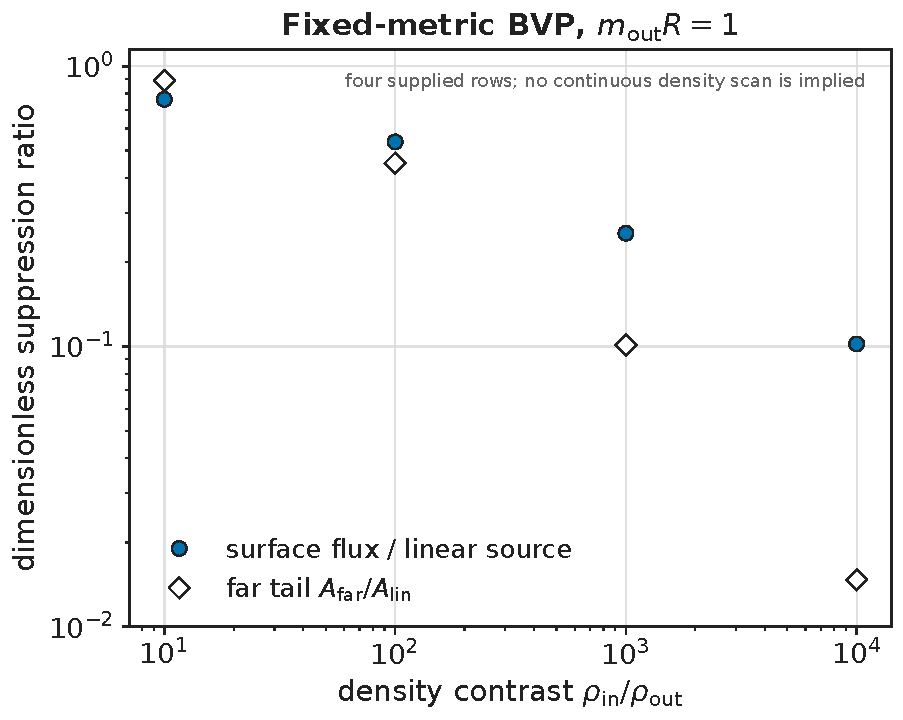
\includegraphics[width=\textwidth,height=0.76\textheight,keepaspectratio]{figures/r154/curve_semantics/nonrotation/fig45_a_fixed_metric_bvp_nodes_r154.pdf}
\caption{Conditional fixed-metric scalar-BVP gate for the four
supplied rows of the named two-slope state at the deliberately artificial
scale $m_{\rm out}R=1$; the four supplied rows are unconnected markers and no
interpolant is implied.  Tail-estimator
definitions are retained as a separate full-width atlas panel, and the
mean-density dimensional gate follows as a continuation.  This is not a
physical body sensitivity, coupled metric, Cassini, WEP or full-PPN
prediction.  Colour is redundant with marker shape, marker fill, luminance
contrast and direct labels; no decorative hatching is used.  \textit{Display semantics: \detokenize{The four supplied fixed-metric BVP rows are shown as unconnected markers; no continuous density scan is implied.}}}
\label{fig:r114_finitebody_scalar_gates}
\end{figure}
\par\smallskip\noindent The fixed-metric tail-estimator detail is retained in Appendix~\ref{app:r129_visual_finite_body_scalar}.

\begin{figure}[p]
\centering
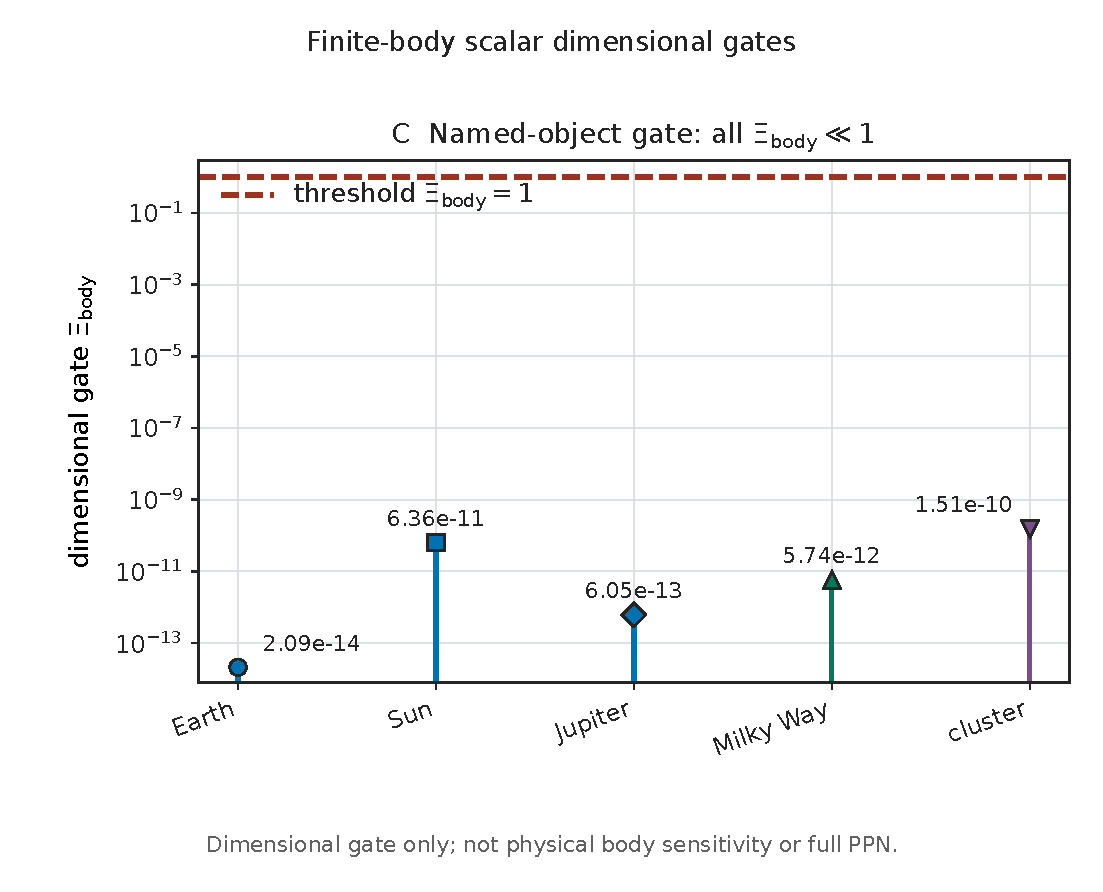
\includegraphics[width=\textwidth,height=0.76\textheight,keepaspectratio]{figures/r148/public_labels/fig45_c_dimensional_gate_public_r148.pdf}
\caption*{\textbf{Figure~\ref{fig:r114_finitebody_scalar_gates}, continued.} Mean-density dimensional gate.  The named state does not reach its formal dense roots; this is not a Cassini, WEP or full-PPN prediction.  Estimator detail remains in the visual atlas.}
\end{figure}
Figure~\ref{fig:r114_finitebody_scalar_gates} groups the three already frozen
finite-body gates without combining their estimators or upgrading their
physical status.

All \(\Xi_{\rm body}\) values are tiny.  The formal high-density equilibrium roots and
their large Planck-factor contrasts are therefore not reached; the actual
linear proxy has \(u=1+O(\Xi_{\rm body})\).  Consequently this named near-GR slice does
\emph{not} obtain a thin-shell or mass-screening suppression from the
displayed scalar mechanism.  Its separately computed unscreened estimate
\(\gamma_{\rm PPN}-1=-0.99998\times10^{-5}\) satisfies only the declared
absolute-deviation proxy gate \(2.3\times10^{-5}\).  Relative to the primary Cassini measurement
\((2.1\pm2.3)\times10^{-5}\)~\cite{Bertotti2003}, the manuscript's
Gaussian standard-error proxy is \(1.35\sigma\) from the central value,
outside the literal one-sigma interval and inside two sigma.  That number is
internal arithmetic, not a significance reported by Cassini, a full
likelihood, or a complete ECT PPN fit.  The
finite-body result is therefore not by itself a local-gravity failure of this
near-GR point.  It also cannot rescue stronger scan points
whose unscreened PPN estimates fail.  Physical body charge, metric
backreaction, \(\beta_{\rm PPN}\), preferred-frame coefficients, composition
dependence/WEP, the two metric potentials and lensing still require the full
coupled finite-body action and remain Open.

This non-uniqueness is constructive rather than merely verbal.  Metric
completions sharing the same tested scalar cone yield
$\gamma_{\rm PPN}=1$, $0$, or $1/3$ depending on the physical metric map, and
the naive direct nonlinear continuation of the scalar completion yields
$\beta_{\rm PPN}=2$.  The latter is excluded at order unity by Solar-System
bounds.  These are kill tests for those named completions, not predictions
that ECT has $\beta_{\rm PPN}=2$ or any one value of $\gamma_{\rm PPN}$.
They prove that the cone and HRC response do not select a Solar-System metric.

The first local acceptance tests are
\begin{equation}
 |\gamma_{\rm PPN}-1|\ll1,
 \qquad |\beta_{\rm PPN}-1|\ll1,
 \qquad |\alpha_{1,2,3}|\ll1,
 \label{eq:ect_cosmo_ppn_gates}
\end{equation}
with the numerical bounds and covariance taken from the chosen current data
release.  A candidate giving an order-unity deviation is killed before it is
tuned to galaxies or cosmology.  Passing PPN does not by itself validate the
cosmological completion; it is a necessary cross-scale gate.

\subsection{External Euclidean response and the outside view}

The outside description is formulated on an interface $\Sigma$ with induced
metric $h_{ij}$, second fundamental form $K_{ij}$ and a specified exterior
operator.  For a massive scalar in a locally flat half-space, the full
flat-boundary Fourier symbol is
\begin{equation}
 \sigma_{\rm flat}(D_E)(x,\xi)=\sqrt{M^2+h^{ij}(x)\xi_i\xi_j}.
 \label{eq:ect_cosmo_dtn_symbol}
\end{equation}
In ordinary classical pseudodifferential calculus its homogeneous principal
symbol is $\sigma_{\rm pr}(D_E)=|\xi|_h$; the mass enters at lower order.
Curvature contributes at subprincipal and lower order through invariants of
$K_{ij}$, derivatives and boundary conditions.  It cannot be inserted into
the flat full symbol as a universal replacement without deriving the operator.

Two exact guards follow.  First, translating a flat interface in ambient
Euclidean space is an isometry, so its DtN spectrum is unchanged; translation
speed is not a Hubble law.  Second, an umbilic embedding of a spatially flat
three-slice in flat $E^4$ with $K_{ij}=(H/c)h_{ij}$ violates the Gauss equation
unless $H=0$.  Non-umbilic embeddings can evade the scalar conclusion only by
introducing directional structure that must be reconciled with observed
isotropy.

The outside view can nevertheless provide a valid owner if a concrete
interface, state and response map are derived from the ordered phase.  It must
then reproduce the internal stress tensor and perturbation operator on shell.
Agreement of the two descriptions is an equality of effective actions or
response kernels, not a visual analogy between a boundary radius and
$c/H$.

\subsection{Unified numerical workflow}

For each candidate completion the following workflow is mandatory.
\begin{enumerate}[label=\textbf{G\arabic*.},leftmargin=*]
 \item Freeze the action, independent variables, constraints, state, boundary
       conditions, conventions and all matching inputs.
 \item Derive the background equations twice: directly by variation and by an
       independent symbolic or Hamiltonian formulation.
 \item Integrate from the derived ordering event; monitor every constraint,
       denominator, response determinant and stability eigenvalue.
 \item Repeat with at least two integration methods and a refinement sequence;
       classify every endpoint before interpreting a time interval.
 \item Derive and reduce the complete quadratic perturbation action on the
       accepted background; scan ghost and gradient eigenvalues over the
       publication $k$--$a$ domain.
 \item Generate recombination, distances, transfer functions and nonlinear
       structure from that same frozen background and physical metric.
 \item Apply observable-specific forward models and likelihoods with nuisance
       parameters, selection functions and covariance.
 \item Publish machine-readable inputs, outputs, hashes, convergence records,
       failure flags and an owner/status ledger.
 \item Run a cross-sector gate: the same completion must pass age, CMB/BAO,
       growth/lensing, cluster and PPN tests without assigning incompatible
       meanings to one parameter.
\end{enumerate}

\paragraph{Two-method background residual.}
For a numerical solution $X(N)$ define
\begin{equation}
 \mathcal R_{\rm bg}=\max_N
 \left\{ {|\mathcal C_0|\over1+\mathcal S_0},
          {\|\mathcal E_A\|\over1+\mathcal S_A},
          {\|X_{(1)}-X_{(2)}\|\over1+\|X_{(1)}\|} \right\},
 \label{eq:ect_cosmo_background_residual}
\end{equation}
where $\mathcal S$ are declared physical scales and $(1),(2)$ label
independent methods.  The acceptance tolerance must be chosen before looking
at observable residuals.  A stable PDF curve without a constraint residual is
not a reproducible cosmological solution.

\paragraph{Frozen scientific payload versus runtime provenance.}
Every numerical row added above is accompanied by a machine-readable input
record, output table, verification script and checksum manifest.  Scientific
payload fields are frozen separately from runtime metadata such as the Python,
NumPy and SciPy version strings.  A cross-version replay that changes only
those metadata strings is a provenance delta, not a scientific disagreement;
conversely, a change in a physical value requires a newly named refreeze and
cannot be hidden by serialization.  Displayed growth ratios are rounded to no
more than thirteen significant digits, below the independent solver agreement.
The finite-window, asymptotic and regular-$r\to1$-limit finite-body statistics retain
separate field names and definitions and must not overwrite one another.

\paragraph{Frozen calculation owners added with this candidate.}
The owner-specific response envelope is generated by
\path{scripts/cosmology/compute_r113_early_response_growth_collapse_envelope.py};
the restricted one-real-pole cluster no-go by
\path{scripts/cosmology/verify_r113_one_pole_cluster_no_go.py};
and the director-source convention audit by
\path{scripts/verification/r113/verify_r113_director_source_normalisation.py}.
Their frozen outputs and checksum manifest reside in
\path{data/cosmology_r113/MANIFEST_SHA256_v3.json}.  The two-slope clock, including
$t(z=10)=0.4814276482$~Gyr under the stated $H_0=67.4$ calibration, is owned
by \path{scripts/cosmology/compute_r103_two_slope_conditional_observables.py}
and \path{data/cosmology_r103/R103_TWO_SLOPE_CONDITIONAL_OBSERVABLES_v1.json}.
These paths become immutable public provenance only when the scripts, data
and manifest are included in the same reviewed repository release as the
manuscript; local file existence alone is not a publication guarantee.

\subsection{Publication products and status transitions}

\begin{longtable}{@{}L{0.17\linewidth}L{0.335\linewidth}L{0.30\linewidth}L{0.115\linewidth}@{}}
\caption{Required publication products for an ECT cosmological completion.}
\label{tab:ect_cosmo_publication_products}\\
\toprule
Channel & Machine-readable product & Scientific acceptance statement & Status now\\
\midrule
\endfirsthead
\toprule
Channel & Machine-readable product & Scientific acceptance statement & Status now\\
\midrule
\endhead
\bottomrule
\endfoot
Action/\allowbreak background & Action record, equations, initial data, $H(a)$, constraints,
response and stability spectra & One globally regular ordered-branch solution
with a physical clock map & A in supplied two-slope action; full ECT owner Open\\
Age & Formation-front congruence/lapse, $H(a)$, dual quadratures and one
dimensional scale calibration & Same physical solution and outside/inside clock agreement &
Conditional $\tau_{2s}$, Gyr clocks and covariance-aware 15-point BC03
calibration computed; full map Open\\
CMB/Hubble & Recombination, transfer functions, spectra, joint covariance & One
early+late likelihood; no duplicated ruler or calibration & Conditional
$r_s$ background diagnostic and one chronometer scale calibration computed;
full inference Open\\
BAO/SN/sirens & $D_M,D_A,D_L,r_{\rm drag},D_L^{\rm GW}$ and nuisance posterior & Physical
photon/tensor metrics and declared distance-duality assumptions & Conditional
background distances computed; full likelihood/tensor owner Open\\
Growth & Reduced quadratic matrices, transfer grid, $f\sigma_8$ likelihood & Stable
physical modes and derived matter coupling on full grid & Restricted
quasistatic diagnostic computed; full result Open\\
Owner-specific $\zeta_{\rm ER}$ envelope & Frozen background, equality,
growth, collapse and rare-tail tables with dual-solver replay & Algebra and
linear growth are Level~A inside the declared envelope; collapse and
Press--Schechter tails are Level~C; no universal ECT parameter is inferred\\
ISW/lensing & $\Phi,\Psi$, kernels, spectra and covariance & Derived Weyl potential
of the physical photon metric & Restricted Weyl/\allowbreak derivative proxy computed;
physical spectra Open\\
JWST & Catalogue intensity, selection, baryonic/halo posterior & End-to-end counts,
masses and morphologies from one completion & Conditional time/\allowbreak volume clocks
computed; abundance/\allowbreak morphology Open\\
Clusters & Time-dependent state, response kernel, mock maps and likelihood &
Hydrodynamic/collisionless evolution plus physical lensing map & Level A
theorem in supplied local map / physical map Open\\
PPN & Finite-body solution and PPN coefficients & Same completion passes local
metric and preferred-frame bounds & A unscreened-family diagnostic; full
finite-body result Open\\
\end{longtable}

A row moves from Open to Level~B when the physical owner and a complete
calculation route are derived but an external matching input remains.  It
moves to Level~C when a declared phenomenological completion is fitted.  It
moves to Level~A only when it is exact in the declared model and assumptions,
with an explicit reproducible derivation; reproducible checks verify that derivation but do not replace it; this does not by itself establish
descent from P1--P6 or physical ECT ownership.  No agreement in one
row promotes any other row automatically.

\subsection{Current terminal conclusions}

The exact results presently available are:
\begin{enumerate}[label=(\roman*)]
 \item the scalar background equations are internally consistent inside their
       declared action;
 \item the current unowned scalar closure is non-identifiable by inverse
       reconstruction, so it does not predict one $H(a)$ or age;
 \item the supplied two-slope action/state has a globally regular conditional
       background, but its coefficients and ordering state are not selected by
       P1--P6;
 \item a strictly increasing local cluster map preserves the set-valued
       argmax and, whenever maxima are attained, cannot displace a total
       response maximizer relative to the supplied total projected baryon
       maximizers; it neither generates the hand-set gas/BCG separation nor
       constrains residual-map extrema;
 \item one constant real Debye pole cannot simultaneously own the declared
       static $a_M$ matching and ballistic $70$--$100$~kpc merger offsets;
       multipole, dispersive and separately owned response kernels remain Open;
 \item a restricted same-metric, zero-slip, sub-horizon closure gives a
       reproducible Weyl-amplitude/\allowbreak derivative proxy for one named state, but
       not a physical ISW or lensing spectrum;
 \item HRC is a quasistatic galactic response candidate and does not replace
       the homogeneous stress, perturbation, photon-metric or PPN owners.
\end{enumerate}
Taken together, corrections A1--A9 close a manuscript-ready audit of the
current cosmological sector: valid conditional results, null results,
tensions, restricted no-go statements and Open owners are all retained.
They do not close a unique or observationally complete ECT cosmology.
The full likelihoods and physical-owner results in the Hubble, age, JWST,
growth, ISW/lensing, cluster-merger and PPN programme remain explicitly
enumerated calculations beyond the conditional diagnostics above.  This conclusion is
stronger and more useful than a common fitted interval: it states exactly
which equations must be derived, which counterexamples already apply, and
which observations can falsify each future completion.

\subsection{Hubble and acoustic calculation}
\label{subsec:ect_cosmo_hubble_acoustic}

\paragraph{Physics of the channel.}
The early acoustic inference constrains the angular and damping scales of a
coupled photon--baryon plasma, while the late ladder constrains calibrated
luminosity distances.  The ECT question is whether one action/state changes
these observables consistently.  It is not whether one background parameter
can be assigned an interval.

\paragraph{Required inputs.}
The calculation requires the physical background and photon metric; baryon,
photon and neutrino densities; the electron mass and binding energies;
Thomson opacity; the primordial state; scalar/vector/tensor transfer
operators; foreground model; late calibrator physics; and the complete
early+late covariance.  Every input is classified as derived, matched,
measured nuisance or Open.

\paragraph{Conditional background calculation now available.}
For each calibrated two-slope orbit, the present bundle computes
\begin{equation}
 r_s^{\rm cond}(z_{\rm drag})=
 \int_{z_{\rm drag}}^{z_{\rm max}}
 {c_{\rm std}\,dz\over
 \sqrt{3[1+R_b^{\rm std}(z)]}\,H_{2s}(z)}
 +r_s^{\rm rad.tail},
 \label{eq:ect_hubble_conditional_rs}
\end{equation}
using a declared standard photon/recombination layer.  This isolates the
effect of the action-owned background and is reproducible, but it is not an
ECT recombination prediction.

\paragraph{Current numerical result.}
Across the nine points of the prespecified \(3\times3\) Cartesian grid,
\(\Delta r_s/r_s\) ranges from \(-0.00323\%\) to \(-30.646\%\).
The largest sampled changes occur where the early long-range response changes by
factors \(1.14\) to \(2.33\) and the unscreened PPN diagnostic fails badly.
The one sampled point satisfying the displayed absolute $\gamma$-proxy gate
changes \(r_s\) by only \(-0.00323\%\).  Thus none of these nine nodes
simultaneously gives a large acoustic shift and satisfies that local proxy;
no statement about unsampled parameter values follows.

\paragraph{Current model-class comparison.}
The distinction is not merely numerical.  In baseline \(\Lambda\)CDM the
early ruler is owned by the standard radiation/matter expansion and
recombination sector; Early Dark Energy~\cite{Poulin2019} changes it through an additional
early component whose perturbations and decay must be evolved; generic
modified-gravity models, including the scalar-tensor/$f(R)$ model class
reviewed in Ref.~\cite{Sotiriou2010}, change it only after their background, photon sector
and gauge-reduced perturbations are specified.  The conditional two-slope
ECT family changes the action-owned background but still imports the standard
photon/recombination layer.  Therefore its displayed \(r_s\) shift is a
background-sensitivity diagnostic, not a completed alternative to any of
those model classes and not evidence of an observational advantage.

\paragraph{Robustness and missing calculation.}
The result must be repeated after deriving the photon metric, recombination
microphysics, finite-body scalar charge and full transfer system.  The
fixed-\(\theta_*\) rescaling in
Table~\ref{tab:two_slope_calibrated_scan_expanded} is deliberately not used
as evidence for a resolved Hubble tension.  The final statistic is one joint
likelihood, not an intersection of separately constructed bands.

\paragraph{Falsifiers.}
A supplied completion fails this channel if it cannot reach recombination
regularly, violates BBN or opacity constraints, produces unacceptable
damping/peak phases, fails the late distance likelihood, or requires
different parameter meanings in the early and late calculations.

\subsection{Chronometer and age calculation}
\label{subsec:ect_cosmo_age_chronometer}

\paragraph{Physics of the channel.}
The observable chronometer relation measures a derivative of population age,
while ECT age is the proper duration of the ordered branch.  Both use the
same matter-clock lapse.  An arbitrary external Euclidean depth is not a
duration; it becomes one only through
Eq.~\eqref{eq:ect_external_depth_lapse_map}.

\paragraph{Current numerical result.}
The named near-GR two-slope completion gives
\(\tau_{2s}\equiv H_{2s}(0)\Delta t=0.9636867786415146\).
Under two disclosed conditional dimensional scale calibrations of that same
dimensionless orbit, it corresponds to \(13.9804960874\) or
\(12.9009506612\) Gyr.  These are not merely arbitrary unit rescalings unless
all physical matter, clock, Planck and recombination scales are co-rescaled.
The absolute-second sound horizon is therefore only a unit-reading diagnostic
until the physical scale map is owned; neither calibration is a second
dynamical orbit.

\paragraph{High-redshift clock outputs.}
Using the externally supplied reference dimensional calibration \(H_0=67.4\), the supplied orbit gives
\(t(z)=1.22645,0.77690,0.48143,0.29241,0.18177\) Gyr at
\(z=4.9,7,10,14.32,20\).  These numbers are calculated from the ECT-candidate
orbit rather than a reference expansion function.  Their scientific status
is conditional on the action/state, photon/matter clock map and scale calibration.

\paragraph{Required observational comparison.}
The chronometer likelihood must propagate stellar population synthesis,
metallicity, star-formation history and covariance.  Absolute-age tests must
propagate object dating and formation priors.  No object older than the
conditional branch age is allowed, but passing this inequality does not
select the action.

\paragraph{Falsifiers.}
A completion fails if a robust object age exceeds its ECT branch age, if the
chronometer derivative is inconsistent with the same \(H(z)\) used for BAO
and supernovae, or if the external-depth/lapse map becomes singular or
state-dependent in a way incompatible with physical clocks.

\subsection{JWST maturity and number-count calculation}
\label{subsec:ect_cosmo_jwst_forward}

\paragraph{Physics of the channel.}
Early massive objects test a product of available time, comoving volume,
initial fluctuations, scale-dependent growth, nonlinear collapse, baryonic
conversion and selection.  A time-budget factor is only one term in that
product.  The current correction therefore replaces the former one-number
extraction by a forward intensity in catalogue space.

\paragraph{Background inputs now available.}
The conditional two-slope orbit supplies \(t(z)\), \(H(z)\), and---under the
declared photon-metric assumption---\(D_M(z)\) and \(dV_c/dz\,d\Omega\).
The nine-node calibrated grid tests whether stronger sampled
scalar-background response helps.  It does not at those nodes: the largest
sampled departure reduces \(t(z=10)\) by \(10.491167\%\), so none of the nine
background nodes enlarges the sampled maturity interval.  Unsampled regions
and the continuous family remain untested.

\paragraph{Perturbative and nonlinear inputs still required.}
The action must predict the primordial covariance and the transfer function
\(T_m(k,z)\).  A validated collapse calculation then generates
\begin{equation}
 {dn_h\over dM_h}(M_h,z)
 =\mathfrak F_{\rm coll}
 [P_m(k,z),\delta_c(z),{\cal E}_{\rm env}],
 \label{eq:ect_jwst_halo_functional}
\end{equation}
where \({\cal E}_{\rm env}\) denotes any derived environmental response.
The stellar relation \(P(M_*,L,\mathcal M|M_h,z)\) and survey selection must
be propagated rather than replaced by a fixed efficiency.

\paragraph{Catalogue statistic.}
For bins \(B_i\) in redshift, mass, luminosity, size and morphology, the
expected counts are
\begin{equation}
 \lambda_i^{\rm ECT}=
 \int_{B_i} dz\,dM_h\,d{\bf y}\,
 {dV_c\over dz\,d\Omega}{dn_h\over dM_h}
 P({\bf y}|M_h,z){\cal S}({\bf y},z),
 \label{eq:ect_jwst_catalogue_intensity}
\end{equation}
and the likelihood includes photometric-redshift, lensing-magnification,
stellar-population and cosmic-variance covariances.  Posterior stellar masses
cannot be treated as model-independent data when the distance map changes.

\paragraph{Morphology and assembly clocks.}
Sizes, Sérsic indices, colours, line widths and merger indicators constrain
assembly histories beyond the scalar age inequality.  The simulation or
semi-analytic model must output these observables at the image level.  A
completion that produces enough halos but cannot produce the observed
morphology remains incomplete.

\paragraph{Current verdict and falsifiers.}
The present ECT result is a direct conditional clock/volume calculation at nine
prespecified nodes; all nine reduce the high-redshift interval relative to the
declared control.  This is not a negative theorem for the continuous
scalar-background family.  Abundance and morphology remain Open.  A separately
declared owner-complete model is falsified by joint failure of its catalogue
likelihood, by an impossible formation time, or by an early-growth enhancement
that violates CMB, lensing or local-gravity constraints.

\subsection{Growth and redshift-space calculation}
\label{subsec:ect_cosmo_growth_rsd}

\paragraph{Physics of the channel.}
Growth is controlled by the full gauge-reduced perturbation action and matter
coupling, not by the background Planck factor alone.  The observable is a
window-convolved anisotropic clustering statistic.  A scalar
\(f\sigma_8(z)\) summary is exact only in the scale-independent limit.

\paragraph{Restricted diagnostic now available.}
For the near-GR named completion, imposing conserved pressureless Jordan
matter, negligible scalar mass/mixing and
\(\mu_{\rm QS}=F_s(0)/F_s(N)\) gives
Eq.~\eqref{eq:two_slope_growth_diagnostic}.  The difference from its matched
control remains below \(1.9\times10^{-3}\%\) through \(z=20\).
This is a Level~C limiting calculation, not the physical ECT growth result.

\paragraph{Restricted peculiar-velocity and bulk-flow carrier.}
With Fourier convention $e^{i\mathbf k\cdot\mathbf x}$ and
$\theta_m\equiv i\mathbf k\cdot\mathbf v_m$, conserved dust in this same
closure obeys
\begin{equation}
 \theta_m=-aHf\,\delta_m,\qquad
 \mathbf v_m(\mathbf k)=i\,aHf\,{\mathbf k\over k^2}\delta_m(\mathbf k).
 \label{eq:ect_restricted_peculiar_velocity}
\end{equation}
For an isotropic real-space window $W_R$, the linear bulk-flow variance is
\begin{equation}
 \langle |\mathbf V_R|^2\rangle=
 { (aHf)^2\over2\pi^2}\int_0^\infty dk\,
 P_{\delta\delta}(k,a)|W_R(k)|^2,
 \label{eq:ect_restricted_bulk_flow_variance}
\end{equation}
before survey geometry, nonlinear velocities and covariance are added.
Using the same primordial normalisation as the restricted growth/Weyl replay,
the carrier $aHfD$ differs from the matched control by
$(0.002894,0.002933,0.002905,0.002821)\%$ at
$z=(0,0.5,1,2)$; its squared-amplitude carrier differs by
$(0.005789,0.005866,0.005809,0.005642)\%$.  Thus this near-GR closure gives
no material enhancement of a Great-Attractor or large-scale-flow signal.
This is a Level~C linear proxy, not a survey bulk-flow prediction: the
primordial spectrum, scale dependence, nonlinear reconstruction, observer
window and velocity likelihood remain Open.  A static galactic HRC map may
not be substituted for the cosmological velocity transfer.  The versioned
replay owners are
\texttt{scripts/cosmology/compute\_r103\_restricted\_isw\_lensing\_proxy.py}
and
\texttt{scripts/cosmology/compute\_r103\_restricted\_large\_flow\_proxy.py}.

\paragraph{Full calculation.}
After constraint reduction, the matter contrast obeys a generally
scale-dependent system
\begin{align}
 D''+\left(2+{H'\over H}+\Gamma_m\right)D'
 -{3\over2}\Omega_m\mu_{\rm cos}(k,a)D
 &=\mathcal S_{\rm mix},\label{eq:ect_growth_full_system}\\
 -k^2\Phi_{\rm W}
 &=4\pi G_Na^2\Sigma_{\rm cos}(k,a)\rho_m\Delta_m.
 \label{eq:ect_growth_weyl_system}
\end{align}
The functions \(\Gamma_m,\mu_{\rm cos},\Sigma_{\rm cos}\) and
\(\mathcal S_{\rm mix}\) are outputs of the physical matrices and vertices.
They cannot be assigned the HRC form.

\paragraph{Likelihood inputs.}
The solver evolves \(P_{\delta\delta},P_{\delta\theta},P_{\theta\theta}\),
constructs the redshift-space multipoles including bias and velocity
dispersion, applies Alcock--Paczynski remapping and the survey window, and
uses the full covariance.  Weak-lensing and CMB-lensing spectra are fitted
jointly because they constrain the same Weyl response.

\paragraph{Current verdict and falsifiers.}
No ECT-native \(S_8\) or \(f\sigma_8\) prediction is claimed.  A completion
fails if it has a ghost/gradient instability, unacceptable scale dependence,
wrong RSD/lensing spectra, or requires a primordial normalisation
inconsistent with its CMB state.  A small background-only or restricted
Weyl-carrier diagnostic cannot rescue such a failure.

\subsection{ISW and lensing calculation}
\label{subsec:ect_cosmo_isw_lensing}

\paragraph{Physics of the channel.}
ISW measures the line-of-sight time derivative of the Weyl potential and
lensing measures its transverse gradients.  The background expansion enters,
but does not determine, either response.  The photon metric and gravitational
slip are indispensable owners.

\paragraph{Transfer calculation.}
For a primordial mode \(\mathcal R({\bf k})\), define
\begin{equation}
 \Phi_{\rm W}({\bf k},z)=
 T_{\rm W}(k,z)\mathcal R({\bf k}),\qquad
 \Phi_{\rm W}'({\bf k},z)=
 T_{\rm W}'(k,z)\mathcal R({\bf k}).
 \label{eq:ect_isw_transfer}
\end{equation}
The same \(T_{\rm W}\) produces CMB lensing, galaxy weak lensing and cluster
lensing.  The derivative \(T_{\rm W}'\) produces the ISW source.  Separate
normalisations for those channels would violate common ownership.

\paragraph{Projected spectra.}
For tracer kernels \(W_X\), the observable spectra have the schematic form
\begin{equation}
 C_\ell^{XY}=4\pi\int {dk\over k}\,
 \mathcal P_{\mathcal R}(k)
 \Delta_\ell^X(k)\Delta_\ell^Y(k),
 \label{eq:ect_projected_spectrum}
\end{equation}
where the transfer kernels include the physical distances and survey
selection.  The ISW--galaxy sign depends on the full time evolution of
\(T_{\rm W}\), tracer bias and redshift distribution; it cannot be inferred
from the sign of a background coupling.

\paragraph{Restricted limiting proxy now available.}
For the named near-GR two-slope state, impose conserved pressureless Jordan
dust, a common matter/photon metric, the sub-horizon quasistatic limit,
negligible scalar mass, mixing and scale dependence, zero slip
$\Phi=\Psi$, the response $\Sigma_{\rm QS}=F_s(0)/F_s(N)$, and the same
primordial growth normalisation in model and control.  With
$\mathcal F=F_s/F_s(0)$ define
\begin{equation}
\begin{aligned}
 Q_{\rm W}^{\rm proxy}
 &= {D\over a\mathcal F},\qquad
 S_{\rm ISW}^{\rm proxy}
 ={aH\over H(0)}{dQ_{\rm W}^{\rm proxy}\over dN},\\
 {d\ln Q_{\rm W}^{\rm proxy}\over dN}
 &=f-1-{d\ln F_s\over dN}.
\end{aligned}
\label{eq:ect_restricted_weyl_isw_proxy}
\end{equation}
Relative to the matched control, the fractional changes are
\[
\begin{aligned}
 Q_{\rm W}&:\ (0.002674,0.002763,0.002825,0.002915)\%,\\
 S_{\rm ISW}^{\rm proxy}&:\ (0.003083,0.003459,0.004256,0.008127)\%,
 \qquad z=(0,0.5,1,2).
\end{aligned}
\]
DOP853/Radau and analytic/finite-difference derivatives
agree at relative levels below $4.3\times10^{-11}$ and
$1.4\times10^{-10}$, respectively.  This is a Level~C restricted-completion
diagnostic.  It is not a prediction of $C_\ell$, weak or CMB lensing, an
ISW angular spectrum, or an ISW--galaxy correlation.  In particular, the
quasistatic assumption removes the horizon-scale dynamics central to ISW.
The versioned publication reproducibility owners are
\path{scripts/cosmology/compute_r103_restricted_isw_lensing_proxy.py}
and
\path{data/cosmology_r103/R103_RESTRICTED_ISW_LENSING_PROXY_v1.json}.

\begin{figure}[p]
\centering
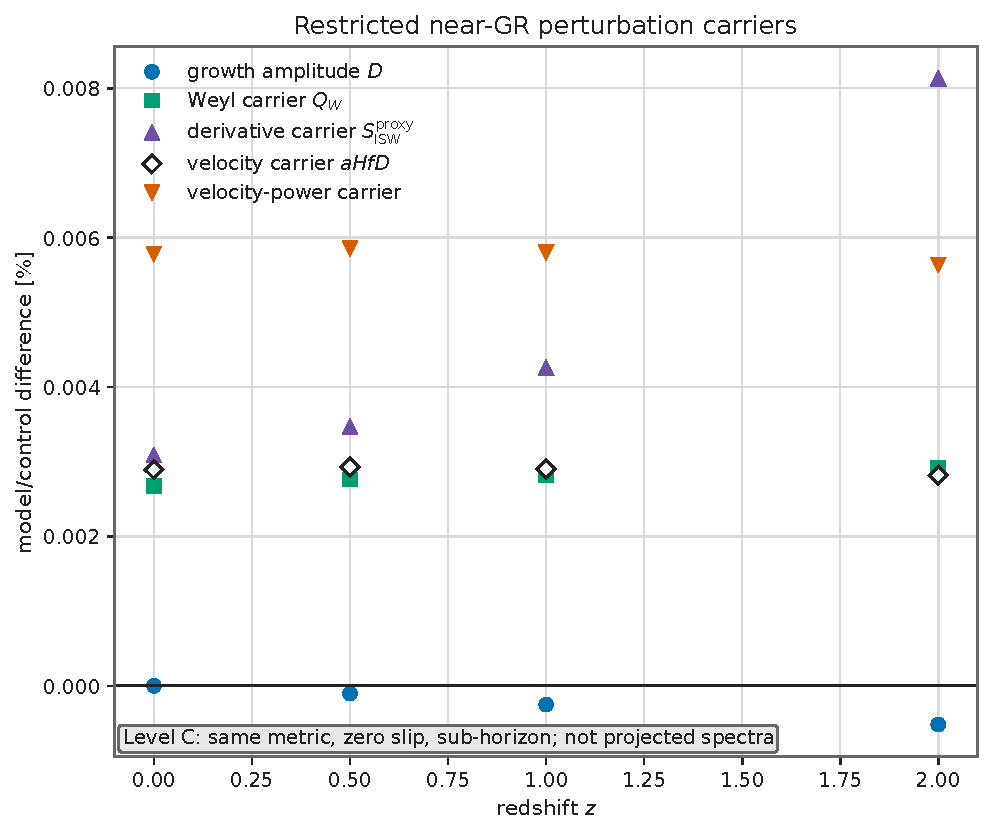
\includegraphics[width=\textwidth,height=0.76\textheight,keepaspectratio]{figures/r153/line_semantics/restricted_perturbation_nodes_r153.pdf}
\caption{Restricted perturbation carriers for the named near-GR two-slope
state relative to its reference control.  The calculation assumes one
matter/photon metric, zero slip, the sub-horizon quasistatic limit, negligible
scalar mass/mixing/scale dependence and a common primordial normalisation.
It is a Level~C limiting diagnostic, not projected ISW, weak/CMB-lensing or
survey bulk-flow spectra.  The four evaluated redshift nodes are unconnected;
no continuous perturbation history or interpolation is implied.  Colour and
marker shape provide redundant encodings.}
\label{fig:r103_ect_restricted_perturbation_proxies}
\end{figure}

Figure~\ref{fig:r103_ect_restricted_perturbation_proxies} displays only the
four evaluated nodes; it does not supply a continuous perturbation history.

\paragraph{Full result still open.}
The supplied two-slope background gives the expansion entering the projection
integrals, but its gauge-reduced perturbation and photon metric are not
derived.  The restricted proxy cannot be upgraded by reusing a reference
transfer function: the physical kernels, spectra and likelihood remain Open.

\paragraph{Falsifiers.}
A completion fails if its Weyl transfer produces the wrong sign or amplitude
of cross-correlations, violates weak/CMB-lensing spectra, or is inconsistent
with the same growth and cluster metric.  Passing background distances alone
does not weaken these tests.

\subsection{Joint multi-observable acceptance}
\label{subsec:ect_cosmo_joint_acceptance}

The programme combines channels at the action/state level.  Let
\(\vartheta_{\rm act}\) be genuine action and state parameters and
\(\nu_i\) observational nuisances.  The joint likelihood is
\begin{equation}
 -2\ln\mathcal L_{\rm joint}(\vartheta_{\rm act},\{\nu_i\})
 =\sum_{ij}
 [d_i-m_i(\vartheta_{\rm act},\nu_i)]
 C^{-1}_{ij}
 [d_j-m_j(\vartheta_{\rm act},\nu_j)]
 \label{eq:ect_joint_owner_likelihood}
\end{equation}
with cross-covariances included.  There is no universal empirical
cosmological drift coordinate and no intersection of probe-specific
intervals in the active theory.

\paragraph{Acceptance hierarchy.}
The order of gates is:
\begin{enumerate}[label=(\arabic*)]
 \item action/constraint consistency and external-depth/lapse ownership;
 \item globally regular background and physical perturbations;
 \item BBN, recombination, photon and local-gravity consistency;
 \item observable-specific forward models;
 \item a joint likelihood and posterior predictive checks.
\end{enumerate}
Failure at an earlier gate is not repaired by a later fit.  Passing one
channel does not promote the status of another.

\paragraph{Figures and tables.}
Publication figures are generated only from action-owned arrays:
background \(H(z)\) and age; distance ratios; recombination and sound
horizon; transfer and growth matrices; Weyl/ISW kernels; JWST forward counts;
cluster retarded-response maps; and finite-body metric residuals.  Until a
listed owner exists, the manuscript provides equations, conditional tables
and explicit empty slots rather than a decorative proxy curve.

\paragraph{Current cross-channel conclusion.}
The supplied two-slope action demonstrates a regular conditional background,
and the nine-node Cartesian grid exposes a sampled early-acoustic/local-gravity
tradeoff.  None of those nine nodes solves the Hubble or early-clock target;
growth, ISW and JWST remain owner-incomplete rather than family-wide negative
results.  The local-HRC theorem separately preserves the possibly empty
set-valued argmax and, whenever maximizers are attained, excludes static
pointwise displacement of a total-response maximizer relative to the
supplied total-baryon maximizers; it does not decide residual morphology or a gas/BCG
separation already present in the input.  These finite-protocol diagnostics and
the separate exact local theorem define the present scope without asserting a
continuous-family no-go.

\section{Conditional force-law effective-dimensionality identity in the HRC-0 point-source diagnostic}
\label{app:deff_method}

\textit{Status: the response algebra is Level~A inside the supplied HRC-0
augmented model; the identity/source bridge is Level~B/Open and this
point-source application is Level~C.  The resulting curve and its mass
independence follow exactly after the HRC-0 response and point-source map
are imposed.  They are not a derivation of G from the microscopic action and are not closure-independent ECT predictions; other
functions share the limiting behaviour only if the same asymptotes are
assumed.}

\subsection{Definition}

For a gravitational force $g(r)$ obeying
$g \propto 1/r^{d-1}$ in $d$ effective dimensions,
the force-law dimensionality is
\begin{equation}
d_{\rm force}(r) = 1 - \frac{d\ln g_{\rm obs}}{d\ln r}\,.
\label{eq:app_dforce_def}
\end{equation}

\subsection{General algebra inside the conditional HRC-0 point-source diagnostic}

Starting from
\begin{equation}
\mu_{g,0}(x^2)\,g_{\rm obs} = g_N(r)\,,
\qquad x \equiv g_{\rm obs}/a_M\,,
\end{equation}
take the logarithmic derivative with respect to $\ln r$:
\begin{equation}
\frac{d\ln g_N}{d\ln r}
= \left(1 + \frac{d\ln\mu_{g,0}}{d\ln x}\right)
  \frac{d\ln g_{\rm obs}}{d\ln r}\,.
\end{equation}
Therefore
\begin{equation}
\frac{d\ln g_{\rm obs}}{d\ln r}
= \frac{d\ln g_N/d\ln r}
       {1 + d\ln\mu_{g,0}/d\ln x}\,,
\end{equation}
and hence
\begin{equation}
\boxed{
d_{\rm force}(r)
= 1 + \frac{p_N(r)}{1 + d\ln\mu_{g,0}/d\ln x}\,,
}
\label{eq:app_dforce_general}
\end{equation}
where $p_N(r) \equiv -d\ln g_N/d\ln r$.

For a point mass, $g_N = G_N M/r^2$ gives $p_N = 2$.

\subsection{Point-source result for $\mu_{g,0}(x^2)=x/\sqrt{1+x^2}$}

Compute:
\begin{equation}
\ln\mu_{g,0} = \ln x - \tfrac{1}{2}\ln(1+x^2)\,,
\qquad
\frac{d\ln\mu_{g,0}}{d\ln x}
= 1 - \frac{x^2}{1+x^2}
= \frac{1}{1+x^2}\,.
\end{equation}
Substituting into~\eqref{eq:app_dforce_general}:
\begin{equation}
\boxed{
d_{\rm force}(x)
= 1 + \frac{2(1+x^2)}{2+x^2}\,.
}
\label{eq:app_dforce_closed}
\end{equation}

\subsection{Limiting cases}

\begin{longtable}{@{}L{3.6cm}L{3.6cm}L{3.6cm}L{3.6cm}@{}}
\toprule
Regime & $x$ & $d_{\rm force}$ & Physics \\
\midrule
\endfirsthead
\toprule
Regime & $x$ & $d_{\rm force}$ & Physics \\
\midrule
\endhead
\bottomrule
\endfoot
High acceleration & $\gg 1$ & $\to 3$ &
  $g \propto 1/r^2$, Newtonian \\
Conditional HRC-0 crossover & $=1$ & $=7/3\approx2.33$ &
  point-source value imposed by $\mu_{g,0}$ \\
Conditional HRC-0 low-acceleration limit & $\ll 1$ & $\to 2$ &
  $g \propto 1/r$, $v_{\rm flat} = \mathrm{const}$ \\
\bottomrule
\end{longtable}

\medskip
Since $v^2=rg$, the exact local identities are
\[
\frac{d\ln v^2}{d\ln r}=2-d_{\rm force},
\qquad
\frac{d\ln v}{d\ln r}=\frac{2-d_{\rm force}}{2}.
\]
The familiar power laws (Keplerian at $d_{\rm force}=3$ and flat at
$d_{\rm force}=2$) apply only where $d_{\rm force}$ is locally or
approximately constant; they are not a global power-law solution through
the varying crossover.

\subsection{Characteristic radius and the true $x=1$ radius}

The reference length
\begin{equation}
r_* = \sqrt{\frac{G_N M}{a_M}}
\end{equation}
is defined by $g_N=a_M$ for the matched conditional HRC-0 scale.  For a
general monotone response,
\begin{equation}
r_{x=1}=\frac{r_*}{\sqrt{\mu(1)}};
\qquad r_{x=1}=2^{1/4}r_*\quad\text{for }\mu_{g,0}(x^2)=\frac{x}{\sqrt{1+x^2}}.
\end{equation}
The conditional HRC-0 script uses the declared matching value
$a_{M0}=1.0824\times10^{-10}\,{\rm m\,s^{-2}}$, giving
$r_*(10^8\,M_\odot)\approx0.36\,$kpc,
$r_*(5\times10^{10}\,M_\odot)\approx8.0\,$kpc, and
$r_*(5\times10^{11}\,M_\odot)\approx25.4\,$kpc.  This is a
bridge-level matched benchmark, not a derivation of $a_M$.

\subsection{Distinction from morphological dimensionality}

The force-law diagnostic $d_{\rm force}$ describes radial scaling inside
the conditional HRC-0 point-source diagnostic and a declared source map.  Morphological
dimensionality instead describes sheets, filaments, and other spatial matter
distributions.  No map from either the conditional HRC-0 point-source response $\mu_{g,0}$ or
the full HRC field problem to a cosmic-web tidal tensor has been derived, so the latter is a
separate Open problem and is not inferred from $d_{\rm force}$.

\subsection{Numerical implementation}

Equation~\eqref{eq:app_dforce_closed} is evaluated analytically for a
point source.  The mapping $x(r)$ uses the exact solution of the conditional HRC-0
point-source relation:
\begin{equation}
g_{\rm obs}^2 =
\frac{g_N^2 + \sqrt{g_N^4 + 4\,g_N^2\,(a_M)^2}}{2}\,,
\qquad x = g_{\rm obs}/a_M\,.
\end{equation}

The versioned implementation is included in the released source package.
Exact reproduction uses the tagged commit and frozen release manifest
associated with the revision, not the moving default branch.


\section{HRC galactic functional and algebraic numerical diagnostic}
\label{app:galactic_phi_closure}

This appendix records the current HRC functional and the reproducible
algebraic SPARC diagnostic.  It does not supply the missing map from the live
$\Phi$ action to the gravitational potential and does not replace the full
three-dimensional disk problem.

\subsection{Variational structure}

After the separate matching in Eqs.~\eqref{eq:hrc_gravity_bridge}
and~\eqref{eq:hrc_identity_bridge}, the static functional is
\begin{equation}
 S_{\rm HRC}^{\rm stat}
 =-\int dt\,d^3x\left[
 \frac{a_M^2}{8\pi G_N}W_g(Y_g)+\rho_b\Phi_{\rm gal}
 \right],
 \qquad
 Y_g=\frac{|\boldsymbol\nabla\Phi_{\rm gal}|^2}{a_M^2}.
 \label{eq:app_gal_functional}
\end{equation}
Variation gives
\begin{equation}
 \boldsymbol\nabla\!\cdot
 \left[\mu_g(Y_g)\boldsymbol\nabla\Phi_{\rm gal}\right]
 =4\pi G_N\rho_b,
 \qquad \mu_g=W_{g,Y_g}.
 \label{eq:app_gal_mu_eq}
\end{equation}
The two registered response laws are
\begin{align}
 \mu_{g,0}(Y_g)&=\sqrt{\frac{Y_g}{1+Y_g}},
 &\mu_{g,3}(Y_g)&=\mu_{g,0}(Y_g)
 \left[1-\frac43\frac{Y_g}{(1+Y_g)^2}\right],
 \label{eq:app_mu_choice}\\
 W_{g,0}(Y_g)&=\sqrt{Y_g(1+Y_g)}-\operatorname{arsinh}\sqrt {Y_g},
 \nonumber\\
 W_{g,3}(Y_g)&=W_{g,0}(Y_g)-\frac83
 \left[\operatorname{artanh}m-m-\frac{m^3}{3}\right],
 &m&=\sqrt{\frac{Y_g}{1+Y_g}}.
 \label{eq:app_F_choice}
\end{align}
Both have the required limits $\mu_g\sim\sqrt {Y_g}$ for $Y_g\to0$ and
$\mu_g\to1$ for $Y_g\to\infty$.  HRC-0 is exact in the augmented
inverse-DtN/recruitment model; HRC-3 additionally assumes the supplied
equal-three-channel rank-one spectral vertex.
The equalities in this registry also assume $s=Y_g$ and $A_g=1$; ERP itself
does not derive that bridge.

\subsection{Symmetry-reduced algebra and the disk guard}

For an isolated spherical configuration,
\begin{equation}
 \mu_{g,k}(g^2/a_M^2)g=g_N,
 \qquad k\in\{0,3\}.
 \label{eq:app_mu_gn}
\end{equation}
The positive solution is unique because both registered responses are
positive and monotone.  HRC-0 can be solved explicitly:
\begin{equation}
 g^2=\frac{g_N^2+\sqrt{g_N^4+4g_N^2a_M^2}}{2}.
 \label{eq:app_final_g_law}
\end{equation}
Equation~\eqref{eq:app_final_g_law} is an HRC-0 identity.  The frozen held-out
HRC-3 path uses deterministic monotone bracketing; the per-galaxy sensitivity
path uses a 60-step safeguarded Newton iteration in $z=g^2/a_M^2$, initialised
by the HRC-0 positive root and protected by a positive half-step fallback.
Their forward residuals are checked on a logarithmic stress grid.  For a
generic disk, the algebraic relation
does not determine the divergence-free curl field and is used only as a
Level-C diagnostic.

\subsection{Baryonic SPARC input}

At each radius the diagnostic uses
\begin{equation}
 V_{\rm bar}^2
 =V_{\rm gas}|V_{\rm gas}|+
 \Upsilon_{\rm d}V_{\rm disk}^2+
 \Upsilon_{\rm b}V_{\rm bul}^2,
 \qquad
 g_N=V_{\rm bar}^2/R.
 \label{eq:app_gn_sparc}
\end{equation}
The sign of the gas component is retained.  Negative total $V_{\rm bar}^2$
rows are excluded from the algebraic inversion and must be handled at the
field/source level in a future solver.

\subsection{Deep branch and BTFR}

For $g\ll a_M$,
\begin{equation}
 g^2\simeq g_Na_M,
 \qquad
 v_\infty^4=G_NM_ba_M.
 \label{eq:app_btfr_again}
\end{equation}
This derives the exponent conditionally.  It does not derive $a_M$, a
redshift law, or the finite-disk normalisation.

\subsection{Possible orientation-sector degeneracy}
\label{app:nlee_galactic_degeneracy}

No orientation source is included.  The live integrability reduction leaves
one longitudinal scalar rather than three independent galactic response
modes.  The three-channel HRC-3 fibre is therefore a supplied response bundle,
not a counted set of live propagating Goldstone modes.  A future covariant
orientation action must be varied and projected before it can alter any curve
or fitted scale.

\section{Computational procedure for the HRC SPARC diagnostic}
\label{app:sparc_computation}

\subsection{Frozen inputs and sample}

The source table is \texttt{MassModels\_Lelli2016c.mrt}.  The diagnostic retains
165 galaxies.  The fixed-$M/L$ mode has 3343 usable physical points after the
declared parsing and positive-source gates.  Whole galaxies, rather than
individual radial points, are assigned to five held-out folds.  Five fixed
seeds test split sensitivity.

\subsection{Fit modes}

The fixed-$M/L$ mode uses $\Upsilon_{\rm d}=0.5$ and
$\Upsilon_{\rm b}=0.7$.  The common-$M/L$ mode fits a shared disk
mass-to-light ratio on the training galaxies and transfers it to the held-out
fold.  Its bound is $0.3\leq\Upsilon_{\rm d}\leq1.0$ and its
parameter-independent validity mask is frozen at the lower bound; this leaves
3342 test points per seed (three excluded from the 3345 parsed rows), rather
than the 3343 points of the fixed-$M/L$ mode.  Neither mode marginalises
distance, inclination, correlated
uncertainties, intrinsic scatter or stellar-population hierarchy.
The velocity objective uses the disclosed floor
$\sigma_{V,i}^{\rm use}=\max(\sigma_{V,i}^{\rm table},2\,{\rm km\,s^{-1}})$;
it must not be described as using the raw table errors without modification.

The separate per-galaxy $M/L$ sensitivity diagnostic uses
$0.1\leq\Upsilon_{\rm d}\leq2.5$ and
$10^{-2}\leq a_M/a_{M0}\leq10^2$, with $\Upsilon_{\rm b}=0.7$ fixed.
It uses a deterministic grid-seeded bounded local optimiser and an independent
differential-evolution audit for every row.  If the local and first global
solutions disagree, two additional fixed seeds are run; verification requires
at least two independently seeded global searches to agree at the lowest
objective within relative tolerance $10^{-7}$.  Boundary hits are reported
rather than interpreted as physical stellar-population estimates.

\subsection{Law registry and inversion}

Only HRC-0 and HRC-3 are registered in the manuscript calculation.  For every
trial $a_M$, the unique positive root of
\begin{equation}
 f(g)=\mu_{g,k}(g^2/a_M^2)g-g_N=0
\end{equation}
is obtained either by monotone bracketing (held-out point registry) or by the
safeguarded $z$-Newton solver above (per-galaxy sensitivity registry).  The two
implementations share the same monotone response and are guarded by a direct
forward-residual test.  The model velocity is
$V_{\rm mod}=\sqrt{gR}$.  The training objective is the declared sum of
squared velocity residuals with the error-floor convention above; the held-out
objective is never used to choose the response law or its fixed HRC-3
coefficient.

\subsection{Reproducibility and interpretation}

The HRC-0/HRC-3 point predictions, per-galaxy contributions, regime
decomposition, fold table and machine-readable result JSON belong to the
versioned HRC numerical reproducibility package.  For a released manuscript
revision, the exact package owner is the corresponding tagged commit and
frozen release manifest; the main-text figures are deterministic renderings
of the files identified there.  HRC-3 was designed after inspection of the
crossover tension, so the present dataset cannot serve as its independent
confirmation.  A prespecified external-galaxy sample is a mandatory next
test.

The current calculation is exact only as an algebraic diagnostic.  A
publication-grade observational result requires the density-aware
axisymmetric PDE, scale heights and boundary conditions, the external field
in the same operator, covariance and hierarchical nuisance marginalisation.


\section{Local-HRC argmax theorem and physical cluster requirements}
\label{app:cluster_lensing}

\textit{Status: the strictly increasing-map order/argmax theorem is
Level~A inside the supplied local map.  The physical cluster source,
response, photon metric, merger dynamics and observational map remain Open.
No hand-set cluster mass, width, offset, critical scale or synthetic replay
is used as ECT phenomenology.}

\subsection{Exact monotonicity theorem}
Let $D$ be the projected domain, let $s(\mathbf x)=\Sigma_b(\mathbf x)>0$,
and define
$\operatorname*{arg\,max}_{D}g=
\{\mathbf x\in D:g(\mathbf x)=\sup_D g\}$, which may be empty.  Let the
proposed static response be $F(\mathbf x)=f[s(\mathbf x)]$ with
$f$ strictly increasing on $s(D)$.  A sufficient smooth condition is
$f\in C^1$ with $f'(u)>0$ for every $u$ in the interval hull of $s(D)$.
Strict monotonicity gives
\begin{equation}
 s(\mathbf x_1)>s(\mathbf x_2)
 \Longleftrightarrow F(\mathbf x_1)>F(\mathbf x_2),
 \qquad \operatorname*{arg\,max}_{D}F
 =\operatorname*{arg\,max}_{D}s.
 \label{eq:cluster_appendix_order_theorem}
\end{equation}
The set identity remains valid when both argmax sets are empty, and the same
ordering argument preserves every isolated local maximum.  Whenever a peak
is attained, no choice of parameters in this strictly increasing positive
local map can move it away from the baryonic proxy that sources it.  A
prescribed input map can only encode an offset already present in its source.

For the explicit local HRC-0 map used in the main text,
Eq.~\eqref{eq:cluster_peak_monotonicity} proves the required positivity,
while Eq.~\eqref{eq:cluster_contrast_compression} shows that the map
compresses contrast.  These exact statements require no synthetic cluster
construction or hand-set numerical input.

\subsection{Required physical calculation}
The physical merger problem is the time-dependent state
$\{\rho_{\rm gas},f_{\rm gal},\rho_*,\Phi,\Psi,\Xi_{\rm resp},
\mathcal K_{\rm ret};\mathbf b,\mathbf v_{\rm rel},t_{\rm obs}\}$.
It requires a derived source vertex and stable causal kernel, a common
matter/photon metric, converged hydrodynamic and collisionless evolution,
and mock-observation likelihoods for shear, convergence, X-ray, SZ and galaxy
maps.  These owners are Open.  Equation~\eqref{eq:cluster_appendix_order_theorem}
prevents a local static rescaling from being mistaken for that calculation.

\subsection{What would count as closure}

A quantitative ECT cluster result must evolve the same action through the
collision, derive the causal response kernel and both matter/photon metrics,
project a mock convergence map, and compare it jointly with shear, X-ray,
SZ and galaxy data including nuisance parameters and covariance.  The local
HRC theorem remains useful as a kill gate: if a proposed implementation is
only a strictly increasing pointwise remapping, it preserves the set-valued
argmax and, whenever maxima are attained, cannot dynamically move a
total-response maximizer relative to its supplied total-baryon maximizers, no
matter how one tunes its scalar scale.  This does not test an inherited
gas/BCG separation or residual-map extrema and is not a no-go for a general
causal merger kernel.

\section{Open calculation of scalar response lengths across environments}
\label{app:screening_benchmarks}

For a declared scalar coordinate~$q$, a homogeneous local linearisation
defines only the conditional response scale
\[
  m_{\rm loc}^2
  =\frac{\mathcal E_{,q}(\bar q,\rho_{\rm m})}{\mathcal A(\bar q)},
  \qquad
  \lambda_{\rm loc}=m_{\rm loc}^{-1},
\]
where $\mathcal A$ and $\mathcal E$ are defined in
eq.~\eqref{eq:phi_eom_local}.  A real positive local Yukawa length requires
the separate conditions $\mathcal A>0$ and $\mathcal E_{,q}>0$; the formula
must not be continued through $\mathcal E_{,q}=0$.  Even when these local
guards hold, this is not yet the canonical finite-body mass or a screening
length measured by a Solar-System experiment.

A quantitative environment calculation must specify:
\begin{enumerate}[label=(\roman*)]
  \item the functions $f,K,V$ and asymptotic background;
  \item canonical Einstein-frame normalisation and Hessian;
  \item regular interior/exterior solutions for each body;
  \item composite-body charge and matching conditions; and
  \item PPN, fifth-force, and equivalence-principle observables.
\end{enumerate}
Until these steps are completed, the density trend and every numerical
response length remain Open.


\section{Operational test of the exploratory environment/history law}
\label{app:aM_environment_test}

This appendix defines a regression protocol for the Open hypothesis~$\Xi$.
It does not assume that $a_{M,\rm eff}$ is non-universal for physical
reasons or that ECT predicts a correlation.

\paragraph{Covariates.}
Environment may be represented by nearest-neighbour density from
2MRS~\cite{Huchra2012}, group membership or host-halo mass from
SDSS~\cite{Yang2007}, tidal-field measures, and explicitly declared history
proxies.  These variables probe different scales and must not be collapsed
into one density without testing that reduction.

\paragraph{Protocol.}
\begin{enumerate}[label=(\roman*)]
  \item fit the conditional HRC rotation-curve diagnostic to obtain
    $a_{M,\rm eff}$ per galaxy;
  \item cross-match the sample to the declared covariates;
  \item regress residuals after controlling for baryonic mass, morphology,
    distance, inclination, and stellar $M/L$;
  \item compare a universal-scale model with prespecified $\Xi$ models using
    held-out or information-criterion tests; and
  \item repeat on gas-dominated and morphology-stratified subsamples.
\end{enumerate}

\paragraph{Interpretation.}
A threshold such as $p<0.01$ may be declared in advance for one analysis, but
it is a statistical decision rule rather than an ECT prediction.  A null
result rejects or constrains the tested $\Xi$ model.  A robust correlation is
an empirical regularity that still requires a microphysical scalar and
screening derivation before it can be attributed to ECT.


% ============================================================
\section{Status, ownership, and falsifiers of the HRC programme}
\label{app:rar_derivation_status}

This appendix prevents three logically different statements from being
collapsed into one: an exact identity inside a supplied response model, a
conditional medium-to-gravity bridge, and an observational diagnostic.  The
current ownership chain is
\begin{align}
 \text{S11a local deformability}+\text{S11b branch reconfigurability}
 &\not\Longrightarrow \text{ERP-$\Phi$},
 \nonumber\\[-2pt]
 \text{S11b branch reconfigurability}
 &\supset \text{ERP-$\Phi$ ideal regime}
 \Longrightarrow \widehat\mu_0(s)\ \text{or}\ \widehat\mu_3(s),
 \nonumber\\[-2pt]
 \widehat\mu_k(s)
 &\xrightarrow[\text{Open}]{\ s=f(Y_g),\ A_g\ }
 \mu_{g,k}(Y_g),\qquad k\in\{0,3\}.
 \label{eq:app_hrc_owner_chain}
\end{align}
S11a says that sufficiently small guarded variations exist; S11b says only
that selected finite transition paths may exist.  Neither derives ERP's equal channels, sharp
threshold, no-hysteresis limit or bounded occupation.  The final arrow is a
separate gravitational matching problem and is not part of any property or
postulate of the pre-geometric $\Phi$-medium.

\subsection{Owner-by-owner status}

\begin{longtable}{@{}L{0.23\linewidth}L{0.28\linewidth}L{0.437\linewidth}@{}}
\caption{Claim ownership in the HRC candidate.  ``Exact'' always means exact
inside the model named in the middle column.}
\label{tab:app_hrc_owner_status}\\
\toprule
Claim & Current owner/status & Missing closure or falsifier \\
\midrule
\endfirsthead
\toprule
Claim & Current owner/status & Missing closure or falsifier \\
\midrule
\endhead
\bottomrule
\endfoot
Infinitesimal local deformability & Conditional Level~A tangent-space result
for regular scalar configurations & Requires fixed admissible boundary data,
regularity margin and topology; it implies neither finite connectivity nor
relaxation \\
Finite branch reconfigurability & Candidate S11b, gravity-free property &
Derive which branches are joined by finite-action paths and whether the
dynamics can traverse them; no universal connectivity is implied \\
Stationary ordered response action & Open / MISSING ACTION; P4 is not a P3
saddle & Close OP-grad or supply one explicit stable P4-supporting action
before identifying a physical constrained Hessian \\
ERP-$\Phi$ & Author-proposed constitutive principle for an ideal symmetric,
quasistatic, additive and non-hysteretic regime & Derive the physical
constrained bundle, equal shift, bounded two-branch occupation and trace
normalisation from a microscopic ordered-phase model; derive a factorised
gap, protected Kubo limit or other exact finite-coupling mechanism \\
Inverse-DtN compliance & Level~A for the stated positive massive Euclidean
half-space problem & Identify the physical interface, boundary condition,
finite-depth and curvature corrections in the live $\Phi$ action \\
Finite-interface infrared limit & Level~A compact periodic-cube counterexample;
smooth HRC density conditional on the continuum-first order of limits &
Identify a noncompact/gapless internal fibre or derive $m_RL$ and quantify the
actual low-spectrum corrections for the physical nonspherical interface \\
HRC-0 primitive and response & Level~A in the augmented
inverse-DtN/recruitment model; Level~B mechanism candidate & Failure of the
three-dimensional spectral density, a residual radial weight, gain/ghost
modes, unavoidable hysteresis or an unprotected finite-probe threshold shift
refutes this completion \\
HRC-3 crossover factor & Level~A in the supplied equal-three-channel rank-one
matrix model; Level~B proof of class & The live scalar-only action does not
provide the required three-channel fibre or equal weights; the coefficient
was selected after the crossover tension was inspected \\
Internal-to-gravity map & Open; represented by $s=f(Y_g)$ and $A_g$ & Exact
HRC gravity additionally assumes $f(Y_g)=Y_g$ and $A_g=1$; a derived
nonidentity map changes the response law \\
Static HRC field equation & Level~A after the supplied gravity functional &
Matter vertex, covariant completion, both metric potentials and
double-counting control remain Open \\
BTFR slope and spherical RAR asymptotes & Exact conditional algebra in the
deep, isolated, spherical branch & The finite-disk normalisation, scatter,
environment dependence and scale owner are not thereby derived \\
$a_{M0}=cH_0/(2\pi)$ & Explicit present-epoch matching condition & The factor
$1/(2\pi)$ and any redshift or memory law remain Open \\
SPARC figures and tables & Level~C held-out algebraic diagnostics & Require a
density-aware axisymmetric PDE, curl field, covariance and hierarchical
nuisance model plus a prespecified independent sample \\
Lensing, clusters, cosmology and PPN & Open in HRC & Require the covariant
metric response and additional tensor/shear, finite-body and dynamical
owners; they are not consequences of the scalar algebraic law alone \\
\end{longtable}

\subsection{Exterior Euclidean check for an arbitrary local interface}

Let $\Sigma$ be a smooth local interface patch, with no assumption about the
global shape of the condensate domain.  For a positive quadratic exterior
operator, minimum-energy continuation of boundary data $\varphi_\Sigma$ into
the adjacent Euclidean region gives
\begin{equation}
 S_{E,\mathrm{on\ shell}}^{(2)}
 =\frac12\langle\varphi_\Sigma,D_E\varphi_\Sigma\rangle,
 \qquad
 D_E=\sqrt{\mathcal L_\Sigma}
 \label{eq:app_hrc_dtn_general}
\end{equation}
at principal-symbol order.  The static compliance is $D_E^{-1}$.  In a local
flat chart with $\mathcal L_\Sigma=-\Delta_\Sigma+m_R^2$, normalising by the
zero-momentum value gives
\begin{equation}
 C(\Lambda)=(1+\Lambda)^{-1/2}.
 \label{eq:app_hrc_dtn_compliance}
\end{equation}
This supplies the compliance factor used by HRC without assuming a spherical
Universe.  It does not supply the released-channel projector, the physical
interface or the map to $Y_g$.  Extrinsic curvature, finite depth, mixed
boundary conditions and anisotropic principal symbols are finite tests, not
optional decorations: a residual spectral weight that destroys the
Newtonian limit falsifies the corresponding interface realisation.

\subsection{Why the current numerical calculation is not yet the field
solution}

For spherical symmetry, integrating the divergence equation gives
\begin{equation}
 \mu_g(g^2/a_M^2)g=g_N.
 \label{eq:app_hrc_spherical_reduction}
\end{equation}
For a disk, the relation instead has the Helmholtz form
\begin{equation}
 \mu_g\boldsymbol g
 =\boldsymbol g_N+\boldsymbol\nabla\times\boldsymbol H,
 \qquad
 \boldsymbol\nabla\cdot
 (\mu_g\boldsymbol g)=4\pi G_N\rho_b.
 \label{eq:app_hrc_disk_helmholtz}
\end{equation}
The curl field depends on the full three-dimensional density, thickness and
boundary data.  Mid-plane component velocities alone do not determine it.
Consequently the present radius-by-radius SPARC computation is an auditable
diagnostic of the response shape, not a completed prediction of disk
galaxies.

\section{HRC stress test with ultra-diffuse galaxies}
\label{app:udg_stress_test}

This appendix gives an HRC-only central-value UDG diagnostic.  It is
deliberately weaker than a spherical or axisymmetric Jeans posterior, but it
exposes the inverse problem and the missing dynamical owners explicitly.

For a pressure-supported system, use the Wolf-type central proxy
\begin{equation}
 R_{1/2}=\frac43R_e,
 \qquad
 M_b(<R_{1/2})\simeq\frac12M_\star,
 \qquad
 g_{\rm obs}=\frac{3\sigma_{\rm los}^2}{R_{1/2}},
 \qquad
 g_N=\frac{G_NM_\star}{2R_{1/2}^2}.
 \label{eq:app_udg_proxy}
\end{equation}
The central inputs and their provenance are
\Needspace*{22\baselineskip}
\begin{table}[H]
\centering
\small
\setlength{\tabcolsep}{4.78pt}
\caption{Inputs of the HRC UDG proxy.  The quoted dispersions are
heterogeneous measurements or literature brackets, not a joint-confidence
sample.}
\label{tab:app_udg_inputs}
\begin{tabular}{@{}L{0.18\linewidth}C{0.11\linewidth}C{0.11\linewidth}C{0.11\linewidth}C{0.11\linewidth}L{0.275\linewidth}@{}}
\toprule
Object & $M_\star/10^8M_\odot$ & $R_e$/kpc &
$\sigma_{\rm los}$/km\,s$^{-1}$ & $\mathcal R_{\rm dyn}$ & Role/status \\
\midrule
NGC~1052--DF4 & 1.50 & 1.60 & $6.3^{+2.5}_{-1.6}$ & 0.787 &
Low-dispersion stress case~\cite{Danieli2022DF4,vanDokkum2018} \\
FCC~224 & 1.74 & 1.89 & $7.8\pm2.0$ & 1.229 &
Stellar-kinematics low-dispersion case~\cite{Buzzo2025FCC224} \\
NGC~1052--DF2 & 1.30 & 2.20 & $8.6$--$14.9$ & 2.328--6.988 &
Ambiguous bracket~\cite{Trujillo2019DF2,Shen2021DF2TRGB,vanDokkum2018} \\
NGC~5846-UDG1 & 1.10 & 2.10 & $17\pm2$ & 10.262 &
Matched-mass control~\cite{Forbes2021NGC5846UDG1} \\
Dragonfly~44\allowbreak\ \cite{vanDokkum2019DF44Kinematics} & 3.00 & 4.70 & $33\pm3$ & 31.734 &
High-dispersion control \\
AGC~114905 & \multicolumn{4}{l}{Gas-rich rotating disk; spherical proxy not applied} &
Axisymmetric solver required~\cite{ManceraPina2022AGC114905} \\
\bottomrule
\end{tabular}
\end{table}

Define $\mathcal R_{\rm dyn}=g_{\rm obs}/g_N$.  A finite positive-$a_M$ HRC
enhancement solution requires $\mathcal R_{\rm dyn}>1$; equality is the
Newtonian boundary $a_M=0$.  Under HRC-0,
\begin{equation}
 \mu_{g,0}(Y_g)=\frac1{\mathcal R_{\rm dyn}}
 \quad\Longrightarrow\quad
 \frac{a_M^{(0)}}{g_{\rm obs}}
 =\sqrt{\mathcal R_{\rm dyn}^2-1}.
 \label{eq:app_udg_hrc0_inverse}
\end{equation}
For HRC-3, monotonicity in the retained rank-one class gives one positive
root $x_3$ of
\begin{equation}
 \mu_{g,3}(x_3^2)=\frac1{\mathcal R_{\rm dyn}},
 \qquad
 a_M^{(3)}=\frac{g_{\rm obs}}{x_3}.
 \label{eq:app_udg_hrc3_inverse}
\end{equation}
The resulting values are reported in Table~\ref{tab:udg_stress_test}.  They
show that a single universal present-epoch scale does not reproduce the
central proxies of all listed systems: one object lies outside the positive
enhancement domain, while the others span effective scales from below one
per cent to nearly five times the matched value.  This is a tension and a
target for a derived environment/history operator, not evidence that such an
operator has already been identified.

The calculation must not be read more strongly than its inputs permit.
Anisotropy, inclination, binary contamination, stellar population, distance,
non-sphericity and selection effects can change the inverse scale.  A complete
UDG result requires posterior propagation through a Jeans or distribution
function model, the same covariant HRC field solver used for ordinary
galaxies, and a predicted incidence distribution rather than a separately
fitted $a_M$ for every object.

\subsection{Jeans upgrade path}
\label{app:udg:jeans_upgrade}

The Wolf proxy suppresses, but does not remove, tracer and anisotropy
dependence.  A forward model must solve
\begin{equation}
 \frac{d(\nu\sigma_r^2)}{dr}
 +\frac{2\beta(r)}{r}\nu\sigma_r^2
 =-\nu(r)g(r),
 \label{eq:app_udg_jeans}
\end{equation}
with $g(r)$ obtained from the same HRC field equation used for ordinary
galaxies.  The projected and aperture-weighted observables are
\begin{align}
 \sigma_{\rm los}^2(R)
 &=\frac{2}{I(R)}\int_R^\infty
 \left(1-\beta\frac{R^2}{r^2}\right)
 \frac{\nu(r)\sigma_r^2(r)r\,dr}{\sqrt{r^2-R^2}},
 \label{eq:app_udg_los}\\
 \langle\sigma_{\rm los}^2\rangle_{\rm ap}
 &=\frac{\int_0^{R_{\rm ap}}WI\sigma_{\rm los}^2R\,dR}
 {\int_0^{R_{\rm ap}}WI R\,dR}.
 \label{eq:app_udg_aperture}
\end{align}
Here $\nu$, $I$, $\beta$, $W$ and the interloper/binary model are nuisance
inputs.  Equations~\eqref{eq:app_udg_jeans}--\eqref{eq:app_udg_aperture}
define the required upgrade; no posterior from them is claimed here.

\subsection{Boundary-aware dispersion-only intervals}
\label{app:udg:nuisance}

At fixed central $(M_\star,R_e)$, propagating only the quoted dispersion
endpoints through the HRC inverses gives Table~\ref{tab:app_udg_intervals}.
These are not common-confidence intervals.  A dash at the low endpoint means
$\mathcal R_{\rm dyn}<1$ and hence no positive-enhancement HRC solution.
\Needspace*{18\baselineskip}
\begin{table}[H]
\centering
\small
\setlength{\tabcolsep}{5.97pt}
\caption{Dispersion-only HRC boundary audit.  Scale ranges are in units of
$a_{M0}$.}
\label{tab:app_udg_intervals}
\begin{tabular}{@{}L{0.18\linewidth}C{0.13\linewidth}C{0.13\linewidth}L{0.225\linewidth}L{0.23\linewidth}@{}}
\toprule
Object & $\sigma$ range & $\mathcal R_{\rm dyn}$ range &
HRC-0 $a_M/a_{M0}$ & HRC-3 $a_M/a_{M0}$ \\
\midrule
NGC~1052--DF4 & 4.7--8.8 & 0.438--1.536 & --- to 0.0380 & --- to 0.0188 \\
FCC~224 & 3.4--14.5 & 0.234--4.248 & --- to 0.309 & --- to 0.282 \\
NGC~1052--DF2 & 8.6--14.9 & 2.328--6.988 & 0.0476--0.470 & 0.0278--0.457 \\
NGC~5846-UDG1 & 15--19 & 7.990--12.819 & 0.572--1.480 & 0.560--1.468 \\
Dragonfly~44 & 30--36 & 26.226--37.766 & 3.381--7.013 & 3.374--7.006 \\
\bottomrule
\end{tabular}
\end{table}
The large ranges show why the central inverse is a stress diagnostic rather
than a population verdict.  Distance, $M/L$, anisotropy, shape, aperture and
membership must be sampled jointly with the physical domain constraint.

\subsection{External field, shape, controls and selection}
\label{app:udg:completion_guards}

HRC currently has no derived external-field operator.  Rough host-field
estimates for DF4, FCC~224, UDG1 and Dragonfly~44 are of the same order as
their internal accelerations in some cases, so an EFE cannot be declared
negligible from $g_{\rm ext}/a_{M0}$ alone.  Its sign and angular structure
must come from the same nonspherical response operator as the disk curl
field; inserting a scalar suppression factor would be another fit law.

FCC~224 has apparent ellipticity $\varepsilon\simeq0.36$
\cite{Buzzo2025FCC224}; its spherical row is therefore only an order-unity
proxy.  The juxtaposition of low-dispersion DF4/FCC~224 with the similarly
diffuse but high-dispersion NGC~5846-UDG1 is a matched-class challenge: a
completion must predict which additional state, history or boundary datum
separates them.  It may not assign an independent $a_M$ after observing the
dispersion.

The known sample is small and selection-biased toward unusual globular
cluster populations.  No selection-corrected observational parent sample is
supplied here, so no population percentage is asserted.  Collision/tidal
channels are external astrophysical alternatives
\cite{Ogiya2018DF2tidal,vanDokkum2022bullet}.  A viable ECT completion must
predict both the conditional kinematics and the incidence/morphology, not
only accommodate individually selected objects.  AGC~114905 supplies a
complementary disk-domain test once the axisymmetric HRC solver exists.


\section{Numerical algorithm for a physical ECT cosmological completion}
\label{app:late_cosmo_algorithm}

The active numerical target is one constraint-preserving integration of a
complete varied ECT action.  A reference background, an independently tuned
growth multiplier, or a manually attached high-redshift tail is not an ECT
solver.

\subsection{Required state and equations}

After gauge reduction the solver state must contain every independent
homogeneous field and its conjugate datum, together with conserved matter and
radiation variables.  At each step it must solve the Hamiltonian constraint,
all evolution equations and all algebraic orientation constraints.  The
minimal diagnostics are
\begin{equation}
 \mathcal G=0,\qquad
 \Delta_F>0,\qquad
 \lambda_{\min}(\mathbf K_{\rm phys})>0,\qquad
 c_{s,i}^2\ge0,
 \label{eq:ect_exact_solver_gates}
\end{equation}
where $\mathcal G$ is the background constraint, $\Delta_F$ denotes every
algebraic denominator and $\mathbf K_{\rm phys}$ is the constrained kinetic
matrix.  Any crossing is a terminal physical failure, not an invitation to
splice in another background.

\subsection{Ordering-to-present integration}

The initial surface is the relational ordering event obtained through the
external-depth/lapse map.  Its state and boundary conditions must be supplied
by the ordering dynamics.  The solver then advances the same equations to
the present, determining \(H(a)\) and the physical normalisation together.
The age is accumulated as an auxiliary quadrature of
Eq.~\eqref{eq:ect_age_ordered_branch}; it is not an input.

\subsection{Constraint reduction and regular variables}

Write the homogeneous equations before elimination as the differential
algebraic system
\begin{equation}
 \mathcal E_A(X,\dot X,H)=0,\qquad
 \mathcal C_\alpha(X,\dot X,H)=0,
 \label{eq:ect_solver_dae}
\end{equation}
where \(\mathcal C_\alpha\) contains the Hamiltonian, unit-director and any
response constraints.  The code first computes the rank of the Jacobian with
respect to the algebraic variables.  On a regular chart,
\begin{equation}
 \det{\partial\mathcal C_\alpha\over\partial Y^\beta}\ne0,
 \qquad Y^\beta=\{H,\lambda_{\rm constr},\ldots\},
 \label{eq:ect_solver_algebraic_rank}
\end{equation}
these variables are solved and substituted into a first-order system in
\(N=\ln a\).  A vanishing determinant triggers a chart change or termination;
it is never regularised by clipping the denominator.

The two-slope scalar implementation uses the state
\begin{equation}
 X=(\sigma,p,\tau,\chi),\qquad
 p={d\sigma\over dN},\qquad
 {d\tau\over dN}={1\over H},\qquad
 {d\chi\over dN}=-{e^{-N}\over H},
 \label{eq:ect_solver_state}
\end{equation}
with \(H\) obtained from the positive Friedmann root at every evaluation.
The age and distance quadratures are therefore integrated by the same
adaptive solver and at the same accepted steps as the fields.

\subsection{Shooting and calibration record}

A named conditional completion may impose terminal calibration targets, but
the shooting variables and targets must be reported separately from theory
inputs and observables.  For the calibrated family the residual is
\begin{equation}
 \mathbf R_{\rm shoot}(\sigma_i,V_{\rm tot})
 =\begin{pmatrix}\sigma(N=0)\\H(N=0)-H_*\end{pmatrix},
 \label{eq:ect_solver_shooting_residual}
\end{equation}
with \(p(N_i)=0\).  A two-dimensional root solve determines
\((\sigma_i,V_{\rm tot})\).  The residual tolerance, Jacobian method,
iteration count and final values are stored in the result file.  A target
such as \(H(0)=H_*\) defines dimensionless units; it does not predict the
observed value of \(H_0\).

The vacuum-ratio condition is checked independently:
\begin{equation}
 {V_-\over V_+}={b_s-2a_s\over2a_s-c_s},
 \qquad
 \left.\partial_\sigma{V_s\over F_s^2}\right|_{\sigma=0}=0.
 \label{eq:ect_solver_vacuum_check}
\end{equation}
Failure of either equality invalidates the declared vacuum calibration even
when the shooting residual is small.

\subsection{Two-integrator and cutoff validation}

Every production orbit is evaluated with an explicit high-order
non-stiff method and an implicit stiff method.  For a quantity \(Q\),
\begin{equation}
 \Delta_Q^{\rm method}=
 {|Q_{\rm DOP853}-Q_{\rm Radau}|\over
  \max(1,|Q_{\rm DOP853}|,|Q_{\rm Radau}|)}
 \label{eq:ect_solver_method_residual}
\end{equation}
is published for the age, terminal state, \(H(0)\), distances and any
integrated acoustic quantity.  Agreement of two methods is a numerical
check, not a physical validation of the action.

The initial-cutoff test repeats the integration at
\(N_i=-20,-30,-40,-60\) where supported.  The missing radiation-era tail is
bounded analytically from the leading radiation solution,
\begin{equation}
 0<\Delta\tau_{\rm tail}
 \le {e^{2N_i}\over2H_0\sqrt{\Omega_{r0}}}
 \left[1+\mathcal O(e^{N_i})\right].
 \label{eq:ect_solver_radiation_tail}
\end{equation}
The bound and the observed cutoff drift are reported separately.

\subsection{Perturbation and observable stages}

Only after the background passes every gate may the same completion generate
the quadratic perturbation operators.  Recombination, distances, transfer
functions, growth, lensing, cluster transport and early-object forward models
are separate downstream stages with frozen inputs and likelihoods.  Their
outputs must carry hashes of the background and action that generated them.

\subsubsection*{Stage P0: background publication}

The frozen background file contains \(N,H,\sigma,\sigma',F,V,\rho_i\), all
algebraic denominators, constraint residuals, age and distance quadratures,
plus the external-depth/lapse variables.  It also carries the action,
parameter, initial-state and source hashes.  Derived interpolation objects
are constructed from this file and never from a separately fitted curve.

\subsubsection*{Stage P1: physical clocks, photons and distances}

The matter-clock and photon metrics are evaluated on the background.
Redshift is computed from the photon energy measured by the matter clock;
the simplification \(1+z=a^{-1}\) is used only after that equality is
verified.  The stage publishes
\begin{equation}
 \{z(N),H_\gamma(z),D_M,D_A,D_L,dV_c/dz\,d\Omega\}
 \label{eq:ect_solver_stage_p1}
\end{equation}
and tests distance duality under its stated assumptions.  This stage is the
owner of chronometer, BAO, supernova and catalogue-volume inputs.

\subsubsection*{Stage P2: thermal and recombination history}

The baryon, photon and neutrino sectors are evolved with their physical
couplings.  The ionisation fraction \(x_e(z)\), optical depth, visibility
function, sound speed, \(r_s\), \(r_{\rm drag}\) and diffusion length are
computed without borrowing a reference expansion.  The imported standard
photon layer used for the conditional two-slope diagnostic is a controlled
test of the background only and is labelled separately in every table.

\subsubsection*{Stage P3: gauge-reduced linear perturbations}

The full quadratic action is reduced before integration.  At every
\((k,N)\) the code records the rank and eigenvalues of the kinetic matrix,
the characteristic speeds, the mass matrix and the source vertices.
Adiabatic and all physical isocurvature modes are initialised in a declared
state.  The transfer file contains
\begin{equation}
 \{T_{\mathcal R},T_m,T_\theta,T_\Phi,T_\Psi,
 T_{\rm vec},T_{\rm tens}\}(k,N)
 \label{eq:ect_solver_transfer_record}
\end{equation}
with gauge-invariant definitions.  A transfer function is not emitted for a
mode whose kinetic term or source vertex is missing.

\subsubsection*{Stage P4: spectra and linear likelihoods}

The transfer functions are convolved with the action-owned primordial state
to obtain matter, velocity, Weyl, CMB and tensor spectra.  Survey windows,
bias parameters and covariance matrices are applied at this stage.  The
pipeline reports both raw theory arrays and residuals in data space so that
normalisation, window and likelihood errors can be distinguished.

\subsubsection*{Stage P5: nonlinear objects and clusters}

Halo collapse and baryonic assembly are simulated or calibrated only after
the linear spectrum is fixed.  JWST number counts and morphologies use the
same distances, volume and time budget as the background.  Cluster mergers
add the retarded response kernel, gas dynamics, collision geometry and
photon metric; the local monotone HRC limit is kept as a negative control.

\subsubsection*{Stage P6: finite-body and local gravity}

The cosmological solution supplies the asymptotic state for an extended-body
boundary-value problem.  The resulting scalar charge and metric are used to
calculate PPN, orbital, time-delay and equivalence-principle observables.
This stage decides whether a cosmologically interesting completion is viable;
screening may not be inserted as a binary flag.

\subsection{Failure taxonomy}

Every failed trajectory receives one primary machine-readable reason:
\begin{longtable}{@{}L{0.20\linewidth}L{0.747\linewidth}@{}}
\toprule
Code & Meaning\\
\midrule
BG-CONSTRAINT & Hamiltonian or algebraic constraint exceeds tolerance\\
BG-SINGULAR & physical reduced denominator or response determinant vanishes\\
BG-GHOST & a physical kinetic eigenvalue becomes non-positive\\
BG-GRADIENT & a physical squared characteristic speed becomes negative\\
MAP-MISSING & matter, photon, tensor or depth/lapse map is not supplied\\
VERTEX-MISSING & a required perturbation or source vertex is absent\\
REC-INCONSISTENT & recombination inputs are not generated by the same state\\
PPN-FAIL & the finite-body completion fails a declared local-gravity gate\\
LIKELIHOOD-OPEN & physical predictions exist but no frozen data likelihood
has been run\\
\bottomrule
\end{longtable}
The first four are failures of the supplied physical completion.  The next
three identify missing ownership.  PPN-FAIL rejects that completion in its
declared local limit.  LIKELIHOOD-OPEN forbids a data-agreement claim but
does not by itself falsify the dynamics.

\subsection{Verification requirements}
\label{sec:late_cosmo_interface}

An accepted implementation must provide: two independent formulations of the
background equations; constraint residuals; convergence under step and
precision refinement; continuation tests near every apparent singularity;
positive-kinetic and gradient checks; a complete input-ownership table; and
reproduction from a frozen environment.  Control solutions may test the code,
but their ages or parameters must never be reported as ECT predictions.

\paragraph{Independent formulation gate.}
The first formulation evolves the reduced first-order system.  The second
evaluates the unreduced Euler--Lagrange and constraint equations on the
interpolated orbit.  Let \(\mathcal E_A^{\rm full}\) denote the latter
residuals.  The report provides
\begin{equation}
 R_A={\max_i|\mathcal E_A^{\rm full}(N_i)|\over
 \max_i[1,|\mathcal T_{A,1}|,\ldots,|\mathcal T_{A,n}|]},
 \label{eq:ect_solver_full_residual}
\end{equation}
where \(\mathcal T_{A,j}\) are the individual equation terms.  A small
reduced-solver error with a large \(R_A\) exposes an elimination or sign
mistake.

\paragraph{Precision and grid gate.}
The integration is repeated with at least two relative/absolute tolerances,
two output grids and two dense-output interpolation orders.  Integrated
quantities are compared before rounding.  A result is quoted to no more
digits than remain stable under all variations and between the two
integrators.

\paragraph{Limit gate.}
The implementation reproduces analytic radiation, matter-tracker and vacuum
limits whenever they exist.  It also reproduces the constant-\(F\) control
after the scalar coupling is disabled.  These tests validate code paths;
they do not make the control cosmology an ECT prediction.

\paragraph{Dependency gate.}
Every downstream file includes the SHA-256 of the exact background input.
A change of action, state, scale calibration, external-depth/lapse map, photon metric
or perturbation operator invalidates all dependent ages, distances, spectra,
figures and likelihoods until they are regenerated.

\paragraph{Counterexample gate.}
The solver suite keeps known negative cases in its private verification
corpus: the local-HRC cluster offset no-go, an unscreened point that fails
Cassini, and a background point with a vanishing response determinant.  A
verification system that accepts any of these as a complete viable
cosmology has failed.

\subsection{Publication artefacts}
\label{sec:late_cosmo_artefacts}

Figures and tables are generated only from a background that passes the exact
solver gates.  The supplied two-slope completion passes the background gates
and therefore owns the conditional tables in
Section~\ref{sec:two_slope_background_proof_class}.  Its restricted growth
and imported-recombination layers remain conditional, while a full Hubble
likelihood, JWST abundance/morphology and gauge-complete growth curve still
await their listed owners.

The minimum frozen release bundle is:
\begin{enumerate}[label=(\roman*)]
 \item action, boundary terms, state and unit/depth-lapse records;
 \item source code and machine-readable environment;
 \item raw background and constraint arrays;
 \item shooting, convergence and independent-residual reports;
 \item photon/recombination and perturbation arrays when present;
 \item every figure source and the exact data array plotted;
 \item likelihood configuration, covariance and residual vectors;
 \item a claim ledger separating Level~A internal results, Level~B
       proof-of-class statements, Level~C conditional comparisons and Open
       owners.
\end{enumerate}

\paragraph{Versioned reproducible artefacts.}
The versioned reproducibility owners contain three independent calculation
products: the named near-GR two-slope orbit and its observables; the nine-point
Cartesian action/state grid with sound-horizon and unscreened-PPN diagnostics;
and the exact local-HRC monotone-map theorem.  None uses a universal empirical cosmological drift
parameter.  The publication source contains the numerical inputs, equations,
assumptions and status of each product; their machine-readable JSON/CSV and
scripts are identified by the frozen release manifest and tagged repository
state.

\section{Conditional loop-scale closures and the remaining first-principles task}
\label{app:Sloop_calc}

\textit{Status: Level~A mathematics for the fixed-length bound and for the
minimum of the explicitly supplied positive-tension 1D functional.  Level~B/Open
as an ECT route because the compact phase, transverse profile, line tension,
unwinding sector and 4D-to-1D reduction are not derived from P1--P6.
CDE-$\Phi$ is only a post-order candidate constitutive hypothesis and
acceptance criterion for a completed branch EFT.  The owner remains the
explicit 4D action, state, profile, vacuum subtraction and physical quotient;
CDE-$\Phi$ is not a theorem or owner of the minimal action.  No
first-principles value of $\hbar$ or universal occupation law is claimed.
Reference from the main text:
Section~\ref{sec:hbar_status}.}

\subsection{Two different reduced-loop closures}

The phase-only Euclidean construction starts from
$\mathcal I_{\theta,E}\sim\int d^4X\,
K_\theta\delta^{AB}\partial_A\theta\partial_B\theta/2$ and introduces the
transverse three-volume weight
$K_\theta^{1\mathrm D}=K_\theta\mathcal A_\perp$.
At fixed loop length $L$ and winding $n$, Cauchy--Schwarz gives
\begin{equation}
 \mathcal I_{\rm loop}(L,n)\ge
 \frac{2\pi^2K_\theta^{1\mathrm D}n^2}{L},
 \label{eq:Sloop_app_phase_bound}
\end{equation}
with equality for uniform winding.  Selecting a core-sized length by hand
defines the phase-only coefficient $\iota_0^{\rm EFT}$ used in the main text.
Because Eq.~\eqref{eq:Sloop_app_phase_bound} tends to zero as $L\to\infty$,
topology and phase stiffness alone do not select a nonzero global reduced
minimum; a physical action additionally requires $\Sigma_\theta$.

The tension-balanced route adds a physically different term.  Suppose a
declared one-dimensional reduced model contains
\begin{equation}
 \mathcal I_n(L)=\mathcal T_{\rm loop}L
       +\frac{2\pi^2K_\theta^{1\mathrm D}n^2}{L},
 \qquad K_\theta^{1\mathrm D}>0,
 \quad \mathcal T_{\rm loop}>0,
 \quad n\ne0.
 \label{eq:Sloop_app_balanced}
\end{equation}
Here $\mathcal T_{\rm loop}$ is the reduced inverse-length coefficient
and is not the chemical potential, a particle mass, or a fitted infrared
cutoff.  In ordinary units
$[K_\theta^{1\mathrm D}]=L$ and
$[\mathcal T_{\rm loop}]=L^{-1}$, so both
$\sqrt{K_\theta^{1\mathrm D}\mathcal T_{\rm loop}}$ and
$\mathcal I_n$ are dimensionless.  The phase-route physical coefficients
are $\Sigma_\theta K_\theta^{1\mathrm D}$ and
$\Sigma_\theta\mathcal T_{\rm loop}$, with dimensions action times length
and action per length.  The natural-unit entries are
$[K_\theta^{1\mathrm D}]=\mathrm{GeV}^{-1}$ and
$[\mathcal T_{\rm loop}]=\mathrm{GeV}$; they do not themselves supply an
action unit.  Interpreting the physical line coefficient as a worldline
rest-action cost or as an ordinary Lorentzian string energy per unit length
requires, respectively, a separately supplied proper-time/state map or a
clock/worldsheet reduction.
Differentiation gives
\begin{equation}
 \frac{d\mathcal I_n}{dL}=\mathcal T_{\rm loop}
 -\frac{2\pi^2K_\theta^{1\mathrm D}n^2}{L^2},
 \qquad
 \frac{d^2\mathcal I_n}{dL^2}=
 \frac{4\pi^2K_\theta^{1\mathrm D}n^2}{L^3}>0.
 \label{eq:Sloop_app_derivatives}
\end{equation}
Together with $\mathcal I_n\to\infty$ for $L\to0^+$ and $L\to\infty$,
this proves
that Eq.~\eqref{eq:tension_balanced_minimum} is the unique global minimum
with respect to $L$, at fixed nonzero winding, inside the supplied
one-coordinate ansatz.  At $L_{*,n}$,
\begin{equation}
 \mathcal T_{\rm loop}L_{*,n}
 =\frac{2\pi^2K_\theta^{1\mathrm D}n^2}{L_{*,n}}
 =\pi|n|\iota_{0,\rm bal}^{\rm eff}.
 \label{eq:Sloop_app_equipartition}
\end{equation}
This equality of the two contributions is why the total balanced coefficient
is twice the phase-only coefficient evaluated at the same selected length,
as stated for the elementary $n=1$ sector in
Eq.~\eqref{eq:S0_bal_fixed_relation}.  For $n=0$, however,
$\mathcal I_{n=0}(L)=\mathcal T_{\rm loop}L$ has infimum zero as $L\to0^+$ and no finite
interior minimum.  Moreover $\mathcal I_{n,\min}=|n|\mathcal I_{1,\min}$, so this two-term
model alone leaves one multiwinding loop marginally degenerate with $|n|$
unit-winding loops; splitting and binding require additional dynamics.

\subsection{Ownership, non-double-counting and falsifiers}

The added term makes a finite conditional minimum possible in the supplied
model.  It is not yet an ECT derivation.  A valid
descent must satisfy all of the following conditions:
\begin{enumerate}
 \item derive the compact $U(1)$ collective coordinate and its admissible
       winding sectors rather than inserting them into the real P3 scalar;
 \item derive $K_\theta^{1\mathrm D}$ and $\mathcal T_{\rm loop}$ from the
       same vacuum-subtracted transverse profile, normalisation and
       coarse-graining map, with a non-overlapping reduction of the form
       $\mathcal I_{\rm 4D,red}^{\rm sub}\to
       \int ds\,[\mathcal T_{\rm loop}
       +K_\theta^{1\mathrm D}(\partial_s\theta)^2/2+\cdots]$, with a
       separate positive physical-action factor, so that the
       longitudinal winding energy is not counted again inside the tension;
 \item derive the correct worldline or worldsheet embedding and its declared
       ensemble, while retaining shape modes, curvature, collapse, splitting,
       self-intersection, radial relaxation and backreaction at the order
       needed to test the full constrained Hessian and whether the minimum
       survives;
 \item test fragmentation and multi-loop channels explicitly: because
       $\mathcal I_{n,\min}=|n|\mathcal I_{1,\min}$, a single $|n|>1$ loop is marginally
       degenerate in the two-term model with $|n|$ separated unit-winding
       loops; the interactions that decide splitting are absent from
       Eq.~\eqref{eq:Sloop_app_balanced};
 \item show that the $n\ne0$ loop cannot unwind through a finite-action path
       excluded by the reduced ansatz;
 \item demonstrate that the resulting scale is independent of arbitrary
       parametrisation, infrared box size and subtraction convention; and
 \item establish cross-sector universality before comparing the candidate
       with the measured $\hbar$.
\end{enumerate}

\subsection{Four-dimensional owner forks}

\paragraph{Codimension-three worldline route.}
The $d^3y$ reduction used in the main text is geometrically consistent with a
localised object on a selected three-dimensional slice whose history is a
curve in the four-dimensional Euclidean carrier.  If its stationary profile
is $\Psi_*^I(y;\vartheta)$ and its physical moduli space contains
$\vartheta\in S^1$, insertion of the slowly varying ansatz into one
vacuum-subtracted action gives
Eq.~\eqref{eq:cde_phi_worldline_reduction}.  In this route,
$\mathcal T_{\rm loop}$ is the reduced inverse-length coefficient and
$K_\vartheta^{1\mathrm D}$ is the positive reduced moduli-space metric.
Only $\Sigma_\vartheta\mathcal T_{\rm loop}$ is the Euclidean physical
action per worldline length, and only
$\Sigma_\vartheta K_\vartheta^{1\mathrm D}$ has dimensions action times
length.  The proper
length $L$ is varied only in a declared closed-worldline/proper-time
ensemble; it is not the texture radius and is external for propagation over
a prescribed duration.  A reparametrisation-invariant representative makes
this ensemble guard explicit.  With $\tau\in[0,1]$, einbein $e(\tau)>0$,
$L=\int_0^1e\,d\tau$ and
$\vartheta(1)-\vartheta(0)=2\pi n$, the leading dimensionless modulus functional is
\begin{equation}
 \mathcal I_{\rm wl}[e,\vartheta]
 =\int_0^1d\tau\left[
   \mathcal T_{\rm loop}e
   +\frac{K_\vartheta^{1\mathrm D}}{2e}
     \left(\frac{d\vartheta}{d\tau}\right)^2
 \right],
 \qquad
 S_{\rm wl,phys}=\Sigma_\vartheta\mathcal I_{\rm wl}.
 \label{eq:t1_einbein_parent}
\end{equation}
The $\vartheta$ equation gives
$K_\vartheta^{1\mathrm D}\dot\vartheta/e=\mathrm{const}$ and therefore
$\dot\vartheta=2\pi n\,e/L$; substitution yields exactly
Eq.~\eqref{eq:t1_vartheta_two_term}.  This proves that the two-term
functional is compatible with worldline reparametrisation invariance.  It
does not make its stationary $L$ physical: the proper-time zero mode must
actually belong to the declared measure or variational ensemble rather than
being gauge or externally fixed.  Any cross-term must be retained unless its
vanishing is proved after the profile equations, constraints, zero-mode
quotient and relaxation are imposed; an informal
``background--fluctuation orthogonality'' is not a substitute for that
calculation.

A three-dimensional texture with nonzero $\pi_3(S^3)$ is the natural
topological candidate for the carrier, while a compact normalisable
collective coordinate can supply the longitudinal phase.  This is not yet a
solution of the live theory.  The minimal two-derivative texture collapses,
and in the static exact-gradient branch
$Q_A=\partial_A\Phi$ with fixed $Q_w=u_0$ the normalised orientation remains
in one contractible hemisphere.  A nontrivial carrier therefore requires
either $w$-dependence, access to $Q=0$, a stabilising higher-gradient term, or
an independent orientation completion.  The carrier charge and the
longitudinal winding must not be identified.

\paragraph{External proof-of-class toy, not an ECT route.}
Standard Skyrme-type models show that an \emph{independent} unit-orientation
field with a separately supplied positive four-derivative operator can evade
the two-derivative Derrick collapse~\cite{Skyrme1961Nonlinear}.  This is only
an external generic-EFT existence analogy.  Before it could enter an ECT
owner chain, the independent field and coefficient would have to be derived
or explicitly supplied, and the actual profile, physical quotient, compact
modulus and constrained Hessian would still have to be solved.  No explicit
Skyrme completion is adopted in the present T1 route.

\paragraph{Codimension-two vortex-worldsheet route.}
A compact $U(1)$ vortex has codimension two.  In four Euclidean dimensions it
is a two-dimensional worldsheet.  A spatial vortex loop that persists for a
$w$-interval $\Delta w$ reduces instead as
\begin{equation}
 S_E=\Delta w\left[
   \tau L+\frac{2\pi^2K_{\rm ws}n^2}{L}+\cdots
 \right].
 \label{eq:t1_worldsheet_fork}
\end{equation}
The bracket is an energy-like functional or action per unit $w$-duration.
Turning it into the worldline action used in
Eq.~\eqref{eq:tension_balanced_loop_functional} requires an explicit clock,
worldsheet state and dimensional reduction.  Consequently an ordinary
vortex ring cannot be used as an unqualified owner of the existing
$\mathcal A_\perp\propto\xi^3$ formula.  Superconducting-string models are an
external example of the additional carrier/internal-current split required
for such a worldsheet route~\cite{Witten1985Superconducting}.

\paragraph{Why constrained orientation does not itself produce a compact
modulus.}
For the minimal scalar, $Q=d\Phi$ leaves a longitudinal real fluctuation
rather than a compact angle.  Rotations that leave one chosen director fixed
rotate an auxiliary transverse frame; without an additional material order
parameter this is basis freedom, not a physical $S^1$.  Moreover a Hopf
circle embedded in $S^3$ is contractible inside the full $S^3$ target.
Therefore compactness must come from the supplied BR1 phase, a physical
collective coordinate of a derived defect, or another explicit completion.
It is not a consequence of integrability alone.  No new foundational
compactness postulate is adopted here: the least invasive conditional test is
whether $\theta|_\Gamma$, or another modulus of an explicit owner solution,
survives as a normalisable physical $S^1$ after the constraint, gauge, frame
and zero-mode quotient.  The longitudinal scalar $\chi$ remains real and is
not identified with that modulus.

\subsection{Elastic completion, shape and splitting}

At fixed $L$, the tension and uniform-winding terms depend only on length;
they do not select shape.  If the same owner yields the positive bending term
in Eq.~\eqref{eq:cde_phi_worldline_reduction}, Fenchel's theorem and
Cauchy--Schwarz give
\begin{equation}
 \oint\mathcal K^2 ds\geq\frac{4\pi^2}{L},
 \label{eq:t1_curvature_bound}
\end{equation}
with equality for a once-covered planar circle.  This proves the circular
minimum inside the positive-bending elastic model and yields
Eq.~\eqref{eq:t1_bending_extension}.  It also shows why the original
two-term value cannot be retained when $\kappa_b$ is material.  The same
equation gives a conditional finite $n=0$ minimum and makes the minimum
nonlinear in $|n|$, thereby lifting the bare splitting marginality even
before profile interactions are restored.

The relation $\mathcal I_{n,\min}=|n|\mathcal I_{1,\min}$ is an exact marginal degeneracy, not
a stability theorem.  Attraction, repulsion and a BPS-like marginal regime
are all possible in admissible completions.  Even repulsion may favour
separated unit-winding carriers rather than selecting one loop.  The sign of
the coincident-core binding term, the allowed splitting channel and the
phase-slip barrier must be computed in the same reduced model.

\subsection{Measure, nucleation and the limited role of PES-R}

The stationary loop of the two-term functional is not automatically a
nucleation bounce.  A semiclassical channel weight has the schematic form
\begin{equation}
 \Gamma_n\sim\mathcal P_n
 \exp\!\left[-\frac{B_n}{S_{\rm measure}}\right],
 \label{eq:t1_nucleation_general}
\end{equation}
where $B_n$ and $S_{\rm measure}$ are independently owned physical actions,
the former has the required bounce and negative mode, and $\mathcal P_n$
contains determinant and zero-mode factors.  The expression
$e^{-2\pi|n|}$ follows only after imposing
$B_n=\Sigma_\vartheta\mathcal I_{n,\min}$,
$S_{\rm measure}=\Sigma_\vartheta
\iota_{0,\rm bal}^{(\vartheta)}$ and an
$n$-independent prefactor.  None of those identifications is derived by the
two-term minimum.

Likewise, a loop-gas proliferation threshold balances physical action
against configurational entropy.  Let $b$ be a declared
lattice/coarse-graining length, $S_{\rm measure}$ the action denominator,
and $\mu$ the connective factor of the specified asymptotic ensemble.  Its
marginality condition is
\begin{equation}
 \frac{\Sigma_\vartheta\mathcal T_{\rm loop}b}{S_{\rm measure}}=\ln\mu .
 \label{eq:t1_loop_gas_marginality}
\end{equation}
Only after independently imposing
$\Sigma_\vartheta\mathcal I_{1,\min}/S_{\rm measure}=2\pi$ does one obtain
\begin{equation}
 \frac{L_*}{b}=\frac{\pi}{\ln\mu}.
 \label{eq:t1_loop_gas_combined_normalisation}
\end{equation}
For representative $\mu=6.774$--$8$, the latter gives
$L_*/b=1.51$--$1.64$ and therefore cannot be evaluated consistently with
the large-loop asymptotics that produced $\mu$; it is also outside a
controlled thin-curve regime when the core width is of order $b$.
Equation~\eqref{eq:t1_loop_gas_combined_normalisation} is thus a UV-control
failure of the combined assumptions, not a continuum prediction or a
derivation of $a_{\rm measure}$, $S_0$ or $\hbar$.  The regulator,
self-avoidance, minimum allowed polygon, curvature and interactions all
remain model data.  PES-R can test an already supplied mode for
admissibility, finite-time retention and record formation.  It neither
supplies the Euclidean measure nor selects exact marginality, and non-normal
dynamics can make an almost marginal mode transiently amplified or noise
dominated rather than robust.

\subsection{Finite acceptance ladder for the T1 programme}

\begin{longtable}{@{}L{0.18\linewidth}L{0.27\linewidth}L{0.43\linewidth}@{}}
\caption{Owner gates for the tension-balanced T1 route.}
\label{tab:t1_owner_gates}\\
\toprule
Gate & Required calculation & Fail condition \\
\midrule
\endfirsthead
\toprule
Gate & Required calculation & Fail condition \\
\midrule
\endhead
\bottomrule
\endfoot
Carrier & Derive a localised finite-action profile and its codimension from
one stationary ordered-phase action & No stationary profile, Derrick
collapse, or mismatch between worldline and worldsheet reduction \\
Length/ensemble & Define worldline proper time versus spatial circumference,
the einbein or parametrisation convention, boundary period, state and
measure; derive the proper-time zero mode and prove why $L$ is varied &
$L$ is an externally prescribed duration, or the einbein zero mode is gauge
or absent from the physical measure \\
Compact modulus & Identify a physical $S^1$ collective coordinate after
quotienting gauge/frame zero modes & The angle is contractible, pure frame
choice, or absent from the physical reduced space \\
Common owner & Compute $\mathcal T_{\rm loop}$ and
$K_\vartheta^{1\mathrm D}$ from the same vacuum subtraction and profile &
Either coefficient is nonpositive, convention dependent, or double counted \\
Projected stability & Evaluate the full constrained Hessian, including
profile relaxation and zero modes & A negative physical mode survives or the
Schur complement is nonpositive \\
Shape & Derive bending and higher-gradient terms & Shape is unstable or the
induced correction invalidates the two-term scale \\
Topology/barrier & Compute phase-slip and carrier-unwinding paths, barrier
and lifetime in a declared state and clock & Any finite path defeats
\emph{absolute} protection; metastability fails only if the calculated
lifetime is below the declared observation window/tolerance \\
Splitting & Compute coincident-core binding and multi-carrier interactions &
The chosen elementary sector fragments or has no isolated state \\
Measure & Derive a bounce, determinant, zero-mode measure and initial state &
The stationary loop is not the relevant saddle or weights are
normalisation dependent \\
PES-R & Supply Lorentzian dynamics, state, width/noise and record protocol &
The mode is inadmissible, too short lived or record incompatible \\
Universality & Compare the same operational action-scale map across at least
two independently normalised sectors & Sector-dependent values or an
uncontrolled matching convention \\
\bottomrule
\end{longtable}

\subsection{Future calculations conditional on closing the owner, profile,
Hessian and barrier gates}

Only after the explicit owner, stationary profile, physical quotient,
projected Hessian and phase-slip/carrier barrier have passed the table above
would the T1 route support applications.  The profile calculation would then
provide a rest-action density
$\mathcal T_{\rm loop}$, an internal inertia
$K_\vartheta^{1\mathrm D}$, a bending modulus and a barrier.  Those outputs
could support the following conditional future tests:
\begin{enumerate}
 \item a Lorentzian Hamiltonian/eigenmode spectrum only after a supplied
       continuation, symplectic structure, operator/domain and state; this is
       not the rejected $e^{-2\pi|n|}$ sector-weight template;
 \item a quantitative phase-slip or unwinding lifetime, rather than an
       assumed topological permanence;
 \item a binding/fragmentation phase diagram comparing a multiwinding
       carrier with separated unit carriers;
 \item a cross-sector universality test of
       $\sqrt{2K_\vartheta^{1\mathrm D}\mathcal T_{\rm loop}}$, using one
       operational normalisation protocol in at least two independently
       derived sectors;
 \item a possible action-scale matching test only if an independently
       normalised source, measure or canonical datum breaks the common
       rescaling degeneracy and the same value is recovered in held-out
       sectors; and
 \item a PES-R application to the derived carrier's poles, widths, transient
       gain, environmental records and survival time.
\end{enumerate}
Failure of the final two items would not erase a sector-specific stable
texture; it would only reject its interpretation as the universal quantum of
action or as a persistent record carrier.

Non-positive coefficients or non-negligible $L$-dependence invalidate the
closed-form minimum above and require the derived functional to be
re-minimised.  Loss of every stable minimum under profile and shape
relaxation, or an admissible finite-action unwinding path, falsifies the
stabilised-loop route.  Sector-dependent values of
$\sqrt{2K_\theta^{1\mathrm D}\mathcal T_{\rm loop}}$ falsify a universal
action scale, but do not by themselves falsify sector-specific loop
stabilisation.  Conversely, a successful 4D solution would upgrade the ownership
of the balanced scale but would still require an independent physical
normalisation and quantum-sector map before $\Sigma_\theta\,\iota_{0,\rm bal}^{\rm eff}=\hbar$
could be claimed.


% ------------------------------------------------------------
\section{Conditional canonical-normalisation result for a supplied
local-CAR fermionic EFT}
\label{app:pauli_exactness}
% ============================================================

\textit{Status: Level~A mathematics conditional on a supplied local
first-order fermionic EFT, positive kinetic coefficient and CAR algebra.
ECT has not derived that fermionic completion from P1--P6.  No universal
curvature-controlled mismatch estimate or astrophysical conclusion is
identified. Open (OP-Q21)
for the full theorem, contingent on the completion of the
fermionic reconstruction programme (OP-Q11). Connections:
\S\ref{sec:qs_statistics} (exchange sectors and spinor
compatibility), \S\ref{sec:qs_dirac} (representation-theoretic
route to Dirac structure), \S\ref{sec:fifth_coupling} (ECT
fermion--condensate coupling $\mu_5$).}

\medskip
This appendix collects the technical material underlying the
provisional no-go statement of
Section~\ref{sec:qs_statistics}: smooth local inhomogeneity does not deform an
already supplied local CAR algebra merely through a positive kinetic
normalisation.  This is not a derivation of Pauli exclusion.  The appendix
proceeds in three steps. First, we
write a representative local first-order fermionic EFT compatible
with the presently identified ECT structures
(\S\ref{app:pauli:eft}). Second, we show that a condensate-dependent
kinetic coefficient is absorbed into a local canonical
normalisation, leaving the equal-time anticommutator in standard
form (\S\ref{app:pauli:normalisation}). Third, we show why the equivalence
principle alone fixes neither curvature-dependent fermion operators nor a
packet-level scaling, so numerical laboratory or compact-object conclusions
are not identifiable without additional owners
(\S\ref{app:pauli:curvature}).

\subsection{General local fermionic EFT on the coherent ordered branch}
\label{app:pauli:eft}

On the smooth coherent ordered branch, a representative local
first-order fermionic EFT compatible with the presently identified
ECT structures---the conditionally supplied Dirac dynamics
(\S\ref{sec:qs_dirac}), medium-ontological identification of
fermionic excitations with spinor modes of the ordered condensate
(\S\ref{sec:fermion_statistics}), and the ECT-specific
preferred-direction coupling
(\S\ref{sec:fifth_coupling})---can be written schematically as
\begin{equation}
\begin{split}
  S_\psi^L\;=\;\int d^4x\,e(x)\,\Bigl[
      &\tfrac{i}{2}\,Z(\phi,n)\,\bar\psi(x)\,\gamma_L^a\,
        e_a{}^\mu(x)\!\stackrel{\leftrightarrow}{D}_\mu\!\psi(x) \\
      &\;-\;M(\phi,n)\,\bar\psi(x)\psi(x) \\
      &\;+\;\mu_5(\phi,n)\,u_\mu(x)
        \bar\psi(x)\gamma_L^\mu\psi(x) \\
      &\;+\;\sum_k C_k(\phi,n)\,\mathcal{O}_k^{(4f)}(x)
      \;+\;\cdots\Bigr],
\end{split}
\label{eq:pauli_app_general_EFT}
\end{equation}
where $e(x)=\sqrt{-\det g_L(x)}$ belongs to a separately supplied
mostly-plus Lorentzian metric/tetrad completion.  Its curved matrices are
$\Gamma^\mu=e_a{}^\mu\gamma_L^a$ with
$\{\Gamma^\mu,\Gamma^\nu\}=-2g^{\mu\nu}$.
The function $Z(\phi,n)$ is smooth and strictly positive,
$M(\phi,n)$ is an effective mass, and
$\mu_5u_\mu\bar\psi\gamma_L^\mu\psi$ is the Lorentzian
preferred-direction operator discussed in Section~\ref{sec:fifth_coupling}.
For the declared future-oriented rest vector it equals $-\mu_5j^0$; the
coefficient sign remains Open.  The $\mathcal{O}_k^{(4f)}$ are local
four-fermion composite operators admitted by the supplied symmetries.

The working assumption of this appendix is that the background
fields are smooth (all spatial and temporal derivatives are finite
and of order the characteristic condensate scales), the kinetic
coefficient is nondegenerate ($Z(\phi,n)>Z_{\min}>0$ and
$e(x)>0$ everywhere in the region of interest), there are no
higher-time-derivative fermionic kinetic pathologies, and no
nonlocal sector-mixing kernels coupling the ordered-branch
fermionic sector to its exterior. These are precisely the
conditions defining ``smooth coherent ordered branch'' for the
purposes of the no-go statement.

\subsection{Canonical normalisation and the equal-time anticommutator}
\label{app:pauli:normalisation}

Extracting the temporal part of the kinetic term
in~\eqref{eq:pauli_app_general_EFT} yields, up to the choice of
local frame and temporal foliation,
\begin{equation}
  \mathcal{L}_{\rm kin}^{(t)}(x)
  \;\sim\;
  i\,\mathcal{K}(x)\,\psi^\dagger(x)\,\partial_t\psi(x)
  \;+\;\cdots,
  \qquad \mathcal{K}(x)>0,
  \label{eq:pauli_app_temporal_kinetic}
\end{equation}
where $\mathcal{K}(x)$ is the resulting smooth and strictly
positive temporal kinetic coefficient, and the ellipsis denotes
terms involving spatial derivatives and mass/interaction pieces
that do not contribute to the equal-time canonical momentum. In
the schematic ECT EFT of
Eq.~\eqref{eq:pauli_app_general_EFT} one has
$\mathcal{K}(x)\sim e(x)Z(\phi(x),n(x))$ up to the choice of
local frame and temporal foliation, so that all statements below
apply to this EFT as a particular case. The canonical momentum
conjugate to $\psi$ is then
\begin{equation}
  \Pi_\alpha(x)
  \;=\;\frac{\partial\mathcal{L}}{\partial(\partial_t\psi_\alpha(x))}
  \;=\;i\,\mathcal{K}(x)\,\psi^\dagger_\alpha(x),
  \label{eq:pauli_app_canonical_momentum}
\end{equation}
and the equal-time canonical anticommutation relation
\begin{equation}
  \{\psi_\alpha(t,\mathbf{x}),\Pi_\beta(t,\mathbf{y})\}
  \;=\;i\,\delta_{\alpha\beta}\,\delta^{(3)}(\mathbf{x}-\mathbf{y}),
  \label{eq:pauli_app_psi_Pi_CAR}
\end{equation}
which in the present normalisation takes the background-weighted
form
\begin{equation}
  \{\psi_\alpha(t,\mathbf{x}),\psi^\dagger_\beta(t,\mathbf{y})\}
  \;=\;\mathcal{K}(x)^{-1}\,\delta_{\alpha\beta}\,
    \delta^{(3)}(\mathbf{x}-\mathbf{y}).
  \label{eq:pauli_app_psi_psi_CAR_weighted}
\end{equation}

Equation~\eqref{eq:pauli_app_psi_psi_CAR_weighted} is the technical
object that a naive gradient-based argument would interpret as a
modification of the exclusion algebra in the presence of a
spatially varying condensate. The correct reading, however, is
that $\psi$ is simply not the canonically normalised field. The
local field redefinition
\begin{equation}
  \chi_\alpha(x)
  \;\equiv\;\mathcal{K}(x)^{1/2}\,\psi_\alpha(x)
  \label{eq:pauli_app_chi_definition}
\end{equation}
brings the kinetic term to canonical form and yields, at equal
times,
\begin{equation}
  \{\chi_\alpha(t,\mathbf{x}),\chi^\dagger_\beta(t,\mathbf{y})\}
  \;=\;\delta_{\alpha\beta}\,\delta^{(3)}(\mathbf{x}-\mathbf{y}),
  \label{eq:pauli_app_chi_CAR}
\end{equation}
which is the standard canonical anticommutation relation in its
unmodified form. Creation operators built from $\chi$ then
satisfy $(\hat a_i^\dagger)^2=0$ mode by mode, and two-fermion
states constructed from them are exactly antisymmetric.

Three comments are in order.

\paragraph{(i) Condensate-dependent mass and preferred-direction
coupling do not alter the exclusion algebra.}
The condensate-dependent mass term $M(\phi,n)\bar\psi\psi$ and
the candidate Lorentzian preferred-direction operator
$\mu_5(\phi,n)u_\mu\bar\psi\gamma_L^\mu\psi$ do not contribute to the
temporal kinetic term~\eqref{eq:pauli_app_temporal_kinetic} and
hence do not modify the canonical momentum or the equal-time
anticommutator. They modify the Dirac operator and the local mode
functions, shifting energies, effective masses, and transport
coefficients, but they do not act on the exclusion algebra
itself.

\paragraph{(ii) Local four-fermion operators modify dynamics, not
statistics.}
Local four-fermion operators
$C_k(\phi,n)\mathcal{O}_k^{(4f)}$ are also absent from the
temporal kinetic term at leading order in the first-order
formulation, and therefore do not modify the canonical momentum
conjugate to $\psi$. They can shift spectra, drive pairing or
condensation phenomena, and modify effective equations of state,
but on the operator-algebra level the fermionic exclusion
structure is fixed by the kinetic term through the canonical
anticommutation relation
(\eqref{eq:pauli_app_chi_CAR}), not by the interaction sector.
This is a standard feature of canonical fermionic field theory.

\paragraph{(iii) Linear gradient contributions cancel for
symmetric packets.}
A naive gradient-based argument would proceed by expanding the
background around a point $\mathbf{x}_0$ and retaining the linear
term $\partial_i\ln\mathcal{K}(x)$. For a symmetrically localised
one-particle wave packet, however, the linear expansion
contributes with vanishing first moment,
$\langle y^i\rangle\equiv\langle(x-x_0)^i\rangle=0$, and the
leading physical correction begins only at second order in the
background inhomogeneity. Furthermore, even this second-order
correction is a packet-level mismatch of mode overlap integrals,
not a violation of the equal-time
anticommutator~\eqref{eq:pauli_app_chi_CAR}.

These three observations close the canonical-normalisation
argument at the level of the present local first-order EFT.

\subsection{Scope of curvature-dependent terms}
\label{app:pauli:curvature}

The equivalence principle permits removal of the connection at a point but
does not determine the allowed curvature-dependent operators in a physical
fermion action.  Such operators may enter at different orders with
independent Wilson coefficients.  Therefore neither a universal packet
mismatch proportional to
$(\mathcal E L^2/c_{\rm char}^2)^2$ nor any compact-object numerical
conclusion follows from the conditional canonical-normalisation argument.

The result established here is narrower: after a smooth, local, invertible
first-order fermionic EFT with the standard CAR algebra is supplied,
canonical normalisation preserves that algebra.  Physical ECT fermions, the
CAR owner, curvature operators and coefficients, states and observable maps
remain Open.  No white-dwarf, neutron-star, VIP-2, Borexino or
Ramberg--Snow comparison is made without those owners.

\subsection*{Relation to the existing fermionic programme}

The no-go statement developed here complements the existing
fermionic programme of the main text in three ways. First, it
combines the exchange-topology classification of
Section~\ref{sec:qs_statistics} with a conditional no-go inside a supplied
local CAR theory.  It neither derives the CAR algebra nor physical fermions
from P1--P6.  Second, it is consistent with a supplied spinorial/Dirac
completion, on which the present canonical-normalisation argument operates.
Third, it
makes explicit the connection between the ECT preferred-direction
coupling, written as $\mu_5u_\mu\bar\psi\gamma_L^\mu\psi$ in the
supplied Lorentzian completion, and the statistics sector of
Section~\ref{sec:fifth_coupling}:
$\mu_5$ contributes to dynamics, not to the exclusion algebra.
The full theorem---unconditional exactness of Pauli exclusion
throughout the coherent branch, or an explicit identification
of the nonlocal, topological-defect, or branch-transition
mechanism responsible for any departures---remains a distinct
target (OP-Q21) contingent on the completion of the fermionic
reconstruction programme (OP-Q11).

% ============================================================
\section{Osterwalder--Schrader spin--statistics test for the free
minimal Euclidean Dirac kernel}
\label{app:q11_os_test}

\textit{Status: Level~A mathematical result (Q11.1a) for
the free minimal Euclidean Dirac kernel, in the conventions of
\S\ref{sec:qs_reflection_positivity}
(eqs.~\ref{eq:q11_eucl_gamma}--\ref{eq:q11_graded_os_form});
the ECT application remains Level~B conditional (Q11.1b).
Connection: \S\ref{sec:fermion_statistics},
\S\ref{sec:qs_reflection_positivity}, \S\ref{sec:dirac_eq}.}

\medskip
Throughout, $m>0$, $\omega(\vec p)=\sqrt{\vec p^{\,2}+m^2}$, and
the reordering rule
\begin{equation}
  \langle\bar\psi_\beta(y)\psi_\alpha(x)\rangle
  =\sigma\,S_{E,\alpha\beta}(x-y),
  \qquad
  \sigma=\begin{cases}-1 & \text{Grassmann},\\
  +1 & \text{commuting},\end{cases}
  \label{eq:q11_reordering}
\end{equation}
is the only point at which the statistics assignment enters
($\sigma$ is local notation of this appendix).
Define the hermitian matrices
$h_\pm(\vec p)=m\gamma_0\pm i\gamma_0\vec\gamma\cdot\vec p$;
hermiticity follows from
$(i\gamma_0\vec\gamma)^\dagger=-i\vec\gamma\gamma_0
=+i\gamma_0\vec\gamma$, and $h_\pm^2=\omega^2$ (cross terms cancel
by $\{\gamma_0,\vec\gamma\}=0$), so
$(\omega\pm h_\pm)/2\omega$ are orthogonal rank-2 projectors.
At the quadratic level the alternative order assignment
$(F,G)=\langle\Theta F\cdot G\rangle$ differs from
\eqref{eq:q11_graded_os_form} by the global reordering sign
$\sigma$ on the elementary families considered below.
The convention \eqref{eq:q11_graded_os_form} is the one for which
both elementary Grassmann families are reflection-positive; the
final identification with standard Euclidean Fermi-field OS
conventions is part of the convention-reconciliation step recorded
at the end of this appendix.

\subsection*{Contour lemma}
For $W>0$ and either sign $s=\pm$:
\begin{equation}
\int\frac{dp_0}{2\pi}\,
\frac{e^{\,is\,p_0W}\,(m-i\gamma_0p_0-i\vec\gamma\cdot\vec p)}
{p_0^2+\omega^2}
=\frac{e^{-\omega W}}{2\omega}\,
\bigl(m+s\,\omega\gamma_0-i\vec\gamma\cdot\vec p\bigr),
\label{eq:q11_contour}
\end{equation}
by closing in the upper ($s=+$, pole $p_0=i\omega$) or lower
($s=-$, pole $p_0=-i\omega$) half-plane.

\subsection*{Grassmann case: both elementary families are
reflection positive}
\emph{Family I.}
$F=\int_{w>0}d^4x\,f^\dagger(x)\psi(x)$, so
$\Theta F=\int_{w>0}d^4y\,\bar\psi(\Theta y)\gamma_0 f(y)$ and
\begin{equation}
Q^{\rm I}[f]
=\langle F\,\Theta F\rangle
=\int\!\!\int d^4x\,d^4y\;
f^\dagger(x)\,S_E(x-\Theta y)\,\gamma_0\,f(y),
\end{equation}
with no reordering (fields already ordered as in the pairing).
Since $x-\Theta y=(w_x+w_y,\vec x-\vec y)$, the contour
lemma~\eqref{eq:q11_contour} with $s=+$ factorises the
$w$-dependence through
$h_f(\vec p)=\int_0^\infty dw\,e^{-\omega w}\tilde f(w,\vec p)$:
\begin{equation}
Q^{\rm I}_{\rm Gr}[f]
=\int\frac{d^3p}{(2\pi)^3}\;
h_f^\dagger(\vec p)\,\mathcal M_{\rm I}(\vec p)\,h_f(\vec p),
\qquad
\mathcal M_{\rm I}
=\frac{(m+\omega\gamma_0-i\vec\gamma\cdot\vec p)\gamma_0}{2\omega}
=\frac{\omega+h_+(\vec p)}{2\omega}\;\ge0 .
\end{equation}
\emph{Family II.}
$G=\int_{w>0}d^4x\,\bar\psi(x)g(x)$, so
$\Theta G=\int_{w>0}d^4y\,g^\dagger(y)\gamma_0\psi(\Theta y)$.
In components,
\begin{equation}
G\cdot\Theta G
=\int\!\!\int d^4x\,d^4y\;
g_\alpha(x)\,g^{*}_{\sigma'}(y)\,(\gamma_0)_{\sigma'\beta}\;
\bar\psi_\alpha(x)\,\psi_\beta(\Theta y),
\end{equation}
and the expectation with the reordering
rule~\eqref{eq:q11_reordering},
$\langle\bar\psi_\alpha(x)\psi_\beta(\Theta y)\rangle
=\sigma S_{E,\beta\alpha}(\Theta y-x)$, gives
\begin{equation}
Q^{\rm II}[g]
=\sigma\int\!\!\int d^4x\,d^4y\;
g^\dagger(y)\;\gamma_0\,S_E(\Theta y-x)\;g(x).
\end{equation}
Here $\Theta y-x=(-(w_x+w_y),\vec y-\vec x)$, so
\eqref{eq:q11_contour} applies with $s=-$ and momentum $\vec q$
conjugate to $\vec y-\vec x$:
\begin{equation}
\gamma_0\,S_E(\Theta y-x)\Big|_{\vec q}
=e^{-\omega W}\,
\frac{m\gamma_0-\omega-i\gamma_0\vec\gamma\cdot\vec q}{2\omega}
=e^{-\omega W}\,\frac{h_-(\vec q)-\omega}{2\omega},
\end{equation}
and after the Fourier transform and relabelling of dummy variables
(the $e^{-\omega w_x}$, $e^{-\omega w_y}$ factors attach to $g(x)$
and $g^\dagger(y)$ respectively, producing the same half-space
profile $h_g$):
\begin{equation}
Q^{\rm II}[g]
=\sigma\int\frac{d^3q}{(2\pi)^3}\;
h_g^\dagger(\vec q)\;
\frac{h_-(\vec q)-\omega}{2\omega}\;
h_g(\vec q).
\end{equation}
For Grassmann fields ($\sigma=-1$):
\begin{equation}
\mathcal M_{\rm II}^{\rm Gr}(\vec q)
=\frac{\omega-h_-(\vec q)}{2\omega}\;\ge0
\quad\text{(orthogonal projector)} .
\end{equation}
The spatial-momentum orientation differs between the families
($h_+$ vs $h_-$); both conclusions are orientation-independent:
positivity is the projector property, and the converse below uses
only $\mathrm{spec}\,h_-=\{\pm\omega\}$.
Extension from the two elementary quadratic families to the full
graded polynomial algebra is the standard OS fermionic construction
and is cited, not re-derived, here.

\subsection*{Commuting case: explicit negative modes}
The strict negative-mode test assumes $m>0$; the massless case
requires separate infrared treatment and is not part of Q11.1a.
Family II with $\sigma=+1$ gives
\begin{equation}
\mathcal M_{\rm II}^{\rm com}(\vec q)
=\frac{h_-(\vec q)-\omega}{2\omega},
\qquad
\mathrm{spec}\,\mathcal M_{\rm II}^{\rm com}
=\{\,0,\;-1\,\}\ \text{(each twice)} .
\end{equation}
\emph{Explicit negative-norm test function.}
Take $\vec q\approx0$, a spinor $u_-$ with $\gamma_0u_-=-u_-$ (so
$h_-(0)u_-=-\omega u_-$), and
$g(w,\vec x)=\chi(w)\rho(\vec x)u_-$ with $\chi$ supported in
$w>0$ and $\rho$ a broad spatial envelope; then
$Q_{\rm com}[g]\to-\,|h_g(0)|^2<0$.
Family I remains positive for $\sigma=+1$ (no reordering occurs
there); reflection positivity nevertheless fails because the OS
form must be non-negative on \emph{all} test functionals.
\emph{Mechanism.}
The statistics assignment enters in exactly one place: the
reordering sign $\sigma$ of \eqref{eq:q11_reordering}.
Grassmann statistics converts the Family-II kernel into the
projector $(\omega-h_-)/2\omega$; commuting statistics leaves
$(h_--\omega)/2\omega$ with spectrum $\{0,-1\}$.
\emph{Diagnostic remark (not part of the proof).}
A separate consistency route would require constructing a positive
commuting Gaussian covariance with spinor indices; if enforcing
ordinary symmetric covariance removes the first-order Dirac
numerator, the resulting object is no longer the same minimal
kernel.

\subsection*{Convention reconciliation and scope}
The conventions of \S\ref{sec:qs_reflection_positivity} lie in the
standard Euclidean Fermi-field OS family
\cite{OsterwalderSchraderFermi1973,Luscher1977,MontvayMunster1994},
with $\gamma_0$ playing the role usually denoted $\gamma_4$.
The reconciliation has been performed at the level of the defining
data and is recorded here.
\emph{(a) Reflection action.}
The trial action
\eqref{eq:q11_eucl_theta_spinor} matches the standard form of
fermionic time reflection used in Euclidean/lattice constructions,
$(\theta\bar\psi)(x)=\gamma_0\psi(\theta x)$,
$(\theta\psi)(x)=\bar\psi(\theta x)\gamma_0$, antilinear and
order-reversing, up to notation and the identification of the
Euclidean time gamma ($\gamma_0$ here, often denoted $\gamma_4$);
see, e.g., \cite{KikukawaUsui2011} for an explicit lattice
Euclidean convention of this reflection type.
\emph{(b) Order and pairing.}
Standard formulations state reflection positivity as
$\langle(\Theta F)F\rangle\ge0$, with action-sign,
measure-ordering, and pairing conventions that vary between
sources, whereas the present free-kernel test uses
$\langle F\,\Theta G\rangle$ with a supplied normalised Berezin Gaussian
($\kappa_F=1$ in the printed covariance convention) and pairing
$\langle\psi\bar\psi\rangle=+S_E$, where here $S_E=D_E^{-1}$ is the
Euclidean Dirac kernel, not an action.  A general finite
$\kappa_F>0$ rescales the covariance and both OS forms by positive factors
without changing the sign verdict; it is a separate source-model owner.
At the quadratic level these two assignments differ by one global
sign from the pairing convention and one from the reordering.
With the order convention \eqref{eq:q11_graded_os_form}, these
signs combine to the same projector-positive branch on the two
elementary Grassmann families analysed above.
This is the global-$\sigma$ equivalence noted at the start of this
appendix.
The page-level comparison with the original OS Fermi-field
constructions, which completes this convention check, is recorded in
item~(c) below.
\emph{(c) Page-level verification (completed).}
The conventions have been verified directly against the original
constructions.
In \cite{Luscher1977}: hermitian Euclidean gamma matrices,
$\{\gamma_\mu,\gamma_\nu\}=2\delta_{\mu\nu}$,
$\gamma_\mu^{\dagger}=\gamma_\mu$ (footnote~5, p.~286, with an
explicit chiral representation in his eq.~(32)); the
reflected-first form
$(\mathcal O_1,\mathcal O_2)
=\langle\theta(\mathcal O_1^{+})\,\mathcal O_2\rangle$ with
the conjugation example $\psi^{+}=\gamma_0\bar\psi$
(eqs.~(4)--(5), p.~284) and Berezin weight $e^{+A}$
(eqs.~(1),(6)); strict positivity for the Grassmann Wilson-fermion
sector (Propositions~1--2, pp.~287--289).
In \cite{OsterwalderSchraderFermi1973}: the doubled-field
construction (\S3.2, pp.~284--285), hermitian Euclidean gammas
$\gamma_{E,\mathrm{src}}^0=\gamma_L^0$,
$\gamma_{E,\mathrm{src}}^j=+i\gamma_L^j$ (p.~282), the
time-inversion involution exchanging the doubled species with the
matrix $\gamma_0$ (eqs.~(4.1)--(4.3), pp.~290--291), the
reflected-first form $\langle X,Y\rangle=(\Theta X,Y)$ with
positivity (Lemma~4.1, p.~292, and \S6), and the explicit remark
that the adjoint of the non-hermitian fermionic action is
implemented by Euclidean time inversion (Introduction, item~III,
p.~278).  Relative to the house map
$\gamma_L^j=i\gamma_{E,\mathrm{house}}^j$, the source uses
$\gamma_{E,\mathrm{src}}^j=-\gamma_{E,\mathrm{house}}^j$ with the
same time gamma.  The two Euclidean representations are unitarily equivalent:
conjugation by $\gamma_0^E$ leaves $\gamma_0^E$ fixed and flips all spatial
gammas.  The order/action-sign differences relative to the present text
reduce to the two global signs documented in (b).
This verification concerns the Euclidean spinor/OS conventions and
the Grassmann reflection-positive branch.
The negative-mode exclusion of the commuting/symmetric alternative
is the explicit free-kernel calculation given above.
The ECT application remains conditional on deriving or verifying
the ECT spinor kernel and spinorial OS structure.
Scope: minimal first-order kernel; $m>0$; pointlike primary-branch
excitations; no higher-derivative kernels;
Majorana/charge-conjugated reformulations would require translating
the reflection matrix and adjoint.
The ECT application (Q11.1b) and the ordered-branch descent (Q11.2)
remain Level~B conditional
(\S\ref{sec:fermion_statistics}).

\section{Unified vacuum-response logic: boundaries, acceleration,
time dependence, and horizons}
\label{app:qs_vacuum_response}
% ============================================================

\textit{Status: Open~(OP-Q12) for the unified ECT response claim.
Each displayed standard/toy calculation can be exact inside its own
supplied assumptions, but a common physical bundle, state, continuation
and coupling that derive all four effects from the reduced ECT action
are missing.}

\medskip
The four effects discussed in
Sections~\ref{sec:qs_casimir}--\ref{sec:qs_unruh}
and~\ref{sec:qs_black_holes}---Casimir-type boundary response, particle
production in time-dependent backgrounds, Unruh-type thermality, and
Hawking-type horizon thermality.  These are supplied comparison targets.
It is Open whether they are probes of one physical ECT response operator.

\subsection*{The unifying logic}

In each supplied calculation the mathematical question is how a stated
state and operator respond when accessibility conditions change:
\begin{enumerate}[label=(\roman*)]
  \item \textbf{Boundary problems:} part of the mode spectrum is
    excluded geometrically; the vacuum response appears as a
    boundary-dependent shift in effective energy~(Casimir-type).
  \item \textbf{Time-dependent backgrounds:} mode definitions at early
    and late times no longer coincide; the mismatch appears as
    Bogoliubov-type particle production.
  \item \textbf{Accelerated observers:} kinematic access to the coherent
    vacuum is restricted observer-dependently; the reduced state takes
    an approximately thermal form~(Unruh-type).
  \item \textbf{Horizons:} division into exterior, shell, and inaccessible
    sectors yields a reduced state after a physical split is supplied.
    Thermality requires an additional state and Hawking-channel owner; a
    partial trace alone does not imply it.
\end{enumerate}

\subsection*{What is and is not claimed}

ECT proposes, but does not yet prove, that these supplied effects can be
obtained from one ordered medium under different restrictions on mode
accessibility and coarse-graining.  Presently they have different
owners: a scalar boundary BVP, a time-dependent mode action, a
Lorentzian QFT state/detector, and a semiclassical strong-field metric.
No stronger common-kernel conclusion follows until those owners descend
from one reduced ECT action.

\subsection*{Analogue-gravity comparison}

Analogue-gravity source models show that effective thermality and horizon
response can arise in ordered media.  This is external mechanism evidence
inside those named models, not a Level-B ECT closure.  The ECT common-response
hypothesis remains Open until one ECT action, state, boundary/detector
operators, observable maps and uncertainty model reproduce the channels and
supply a discriminator against their separate standard owners.

\section{Bath regimes, effective spectral structure, and the limits
of the ohmic/Markov closure}
\label{app:qs_bath_regimes}
% ============================================================

\textit{Status: standard reduced-state bookkeeping for a declared
channel; Level~A only for algebra within the specified quadratic source
model; Open for the ECT split, vertices, state, and quantitative bath
interpolation (OP-Q15).}

\medskip
This appendix clarifies the status of the effective bath description used
in Section~\ref{sec:qs_decoherence}.
The main text employs a reduced influence-functional language in which a
subsystem of coherent variables interacts with an effective environment.
Such a split may be supplied after coarse-graining over selected coherent
and topological degrees of freedom, but the physical subsystem/environment
map and detailed bath model remain an effective closure rather than a first-principles
theorem from bare~P3.

\subsection*{Effective spectral density}

The central quantity is the Weiss-normalised effective spectral density
$J_W(\omega)$, which determines dissipation and noise kernels in the reduced
dynamics.  It is distinct from the bare mode-density weight by
$J_W(\omega)=J_{\rm bare}(\omega)/(2\omega)$ in the convention fixed in
Appendix~\ref{app:AP6A-conventions-kernels}.
In the simplest closure one assumes a smooth positive spectral density
and, in the many-mode regime, an effectively Markovian coarse-grained
behaviour.
For a supplied three-dimensional soft-coordinate bath with derivative
coupling, mode counting gives $J_{\rm bare}(\omega)\propto\omega^4$ and
therefore $J_W(\omega)\propto\omega^3$.  This is Level~A conditional
mathematics inside that supplied bath model, not a derivation of a physical
ECT bath, vertex or record channel.
The effective ohmic/Markov approximation is a model ansatz.  The
general entropy-rate identity~\eqref{eq:qs_entropy_explicit} has no fixed sign
until the reduced generator and state are supplied.

\subsection*{Two regimes}

Two regimes must be kept distinct:

\paragraph{Strong declared record channel.}
When the physical record differences and noise kernel make $\Phi_{ab}(T)$
large, off-diagonal reduced-state terms are strongly suppressed and records
can become robust.  The total mode count alone does not ensure this, and
entropy monotonicity still requires a channel theorem.

\paragraph{Weak bath: $N_{\rm eff}\sim 1$.}
When only very few effective environmental channels are active, coherent
recurrences, partial reversibility, and incomplete decoherence remain
possible.
This is the regime in which the subsystem retains recognisably quantum
behaviour~(Section~\ref{sec:qs_decoherence}).

{\small
\renewcommand{\arraystretch}{1.3}

\begin{longtable}{@{}L{3.5cm}L{4.5cm}L{3.5cm}L{3.0cm}@{}}
\caption{Declared reduced-channel regime summary.}\label{tab:bath_regimes}\\
\toprule
Regime & Effective condition & Behaviour & Status \\
\midrule
\endfirsthead
\toprule
Regime & Effective condition & Behaviour & Status \\
\midrule
\endhead
\bottomrule
\endfoot
Weak declared record channel & Small pairwise $\Phi_{ab}(T)$
  & Coherence may persist or revive; mode count alone is insufficient
  & Source-model / ECT Open \\
Strong declared record channel & Large pairwise $\Phi_{ab}(T)$
  & Selected off-diagonal terms are suppressed; entropy sign is not fixed
  & Source-model / ECT Open \\
Conditional entropy theorem
  & Declared unital, detailed-balance, or contractive channel plus state and
    entropy functional
  & Monotonicity only for the named functional under its hypotheses
  & Standard conditional theorem / ECT Open \\
\bottomrule
\end{longtable}
}

\subsection*{Open problem}

Generic subsystem--environment bookkeeping exists for a declared
source model.  What remains Open in ECT is the physical split, interaction
vertices, record operators, state, noise kernel, reduced map, and entropy
functional.  Only after these are derived can a bath hierarchy or monotone
entropy theorem be tested (OP-Q15/OP-Q17).

% ============================================================

% ============================================================
% ============================================================
\section{Mathematical apparatus for conditional decoherence calculations
and future ECT record-channel tests}
\label{app:decoherence_apparatus}
% ============================================================

\textit{Status: Level~A conditional mathematics / Level~B calculational
apparatus for a supplied subsystem--bath model; physical ECT ownership is
Open.  The generic Weiss spectral-density family, the noise and dissipation kernels,
and the decoherence exponent are constructed only after a split, free bath,
vertex and state are supplied.  The specific exponent is parameterised rather
than fixed by the live ECT action.}

This appendix should be read as an operational extension of
Appendix~\ref{app:qs_bath_regimes}.
The earlier appendix classifies the admissible bath regimes and the
status of the ohmic/Markov closure; the present appendix supplies a
generic calculational toolkit within that closure language.
It does not upgrade the bath model to a first-principles theorem from
bare~P3.

% ------------------------------------------------------------------
\subsection{Generic subsystem--bath coupling class}
\label{app:M1_coupling}

As a generic reference calculation, suppose a supplied three-dimensional
free bath has $N_G=3$ independent linearly dispersing coordinate fields,
$\omega_k=c_{\rm char}|\mathbf{k}|$.  This is the naive unconstrained
orientation-bath benchmark, not the integrability-reduced physical spectrum
of the live ECT action (Section~\ref{sec:goldstone_integrability_main}).
For a localised subsystem with generalised coordinate~$q$, a separately
supplied coupling to these modes takes the generic form
\begin{equation}
  H_{\rm int} = q \sum_{\alpha} g_\alpha(\mathbf{k}_\alpha)\,
  \chi_\alpha(\mathbf{x}_q),
\end{equation}
where $g_\alpha(\mathbf{k})$ is the coupling vertex.  No such physical ECT
record vertex, resolved/unresolved split or bath state is identified here.

The bare mode-density weight and the Weiss/Feynman--Vernon spectral density
must be kept distinct:
\begin{equation}
  \label{eq:J_generic_family}
  \boxed{
  J_{\rm bare}(\omega)
  = \mathcal{A}_{\rm b}\,\omega^2
    |g(\omega/c_{\rm char})|^2 e^{-\omega/\omega_c},
  \qquad
  J_W(\omega)=\frac{J_{\rm bare}(\omega)}{2\omega},
  \qquad
  \omega_c \sim c_{\rm char}/\xi_{\rm cond}.
  }
\end{equation}
The estimate $\omega_c\sim c_{\rm char}/\xi_{\rm cond}$ is only a
Level~C/parametric matching ansatz for this supplied source model.  Neither
the physical cutoff nor the dimensionful $c_{\rm char}$ is owned by the live
ECT action.  Here $\xi_{\rm cond}$ denotes a separately declared bath cutoff
length; it is not identified with $\xi_{\rm P3}$, an Open P4 pole length, or a
universal condensate scale.
Within this fixed $d=3$, $z=1$, canonically normalised coordinate-field
benchmark, the remaining exponent shift is controlled by the declared
coupling vertex.  In general it also depends on the physical mode projector,
dispersion, dimensionality, canonical normalisation, degeneracy and infrared
structure:
\begin{itemize}
  \item density coupling, $g(k)\sim\mathrm{const}$:
    $J_{\rm bare}(\omega)\propto\omega^2$ and
    $J_W(\omega)\propto\omega$ (ohmic in the standard CL classification);
  \item derivative coupling, $g(k)\propto k$:
    $J_{\rm bare}(\omega)\propto\omega^4$ and
    $J_W(\omega)\propto\omega^3$ (super-ohmic in the supplied
    three-dimensional coordinate-field bath with gradient interaction ---
    this is the regime identified in the main text,
    eq.~\eqref{eq:qs_super_ohmic});
  \item an effective ohmic law $J_W(\omega)\propto\omega$ can arise from
    the constant-coupling benchmark in this declared normalisation, or from
    additional coarse-graining/reduced dimensionality applied to another
    vertex.  No such physical ECT vertex is selected by
    eq.~\eqref{eq:qs_ohmic}.
\end{itemize}
To maintain generality, the subsequent formulae are written for the
generic Weiss power-law family
\begin{equation}
  \label{eq:J_s_generic}
  J_s(\omega)\equiv J_W(\omega)
  = A_s\,\omega^s\,e^{-\omega/\omega_c},
\end{equation}
with $A_s\geq0$, $\omega_c>0$ and $s>0$.  The direct examples are
$s=1$ (ohmic constant-coupling benchmark) and $s=3$
(super-ohmic derivative-coupling benchmark) as the two direct cases above;
other $s>0$ remain admissible supplied effective families.  None is thereby
selected as the physical ECT record channel.

% ------------------------------------------------------------------
\subsection{Symmetrised force kernel $C_H(\tau)$ and
action-normalised noise $N(\tau)$}
\label{app:M2_noise_kernel}

Given the Weiss spectral density~\eqref{eq:J_s_generic}, suppose first that
the stationary Gaussian oscillator bath is in a declared thermal/KMS state at
$T_{\rm eff}$ (with $k_B=1$).  Its physical symmetrised bath-force correlator
and the action-normalised noise kernel are
\begin{equation}
  \label{eq:N_tau_general}
  \boxed{
  C_H(\tau)
  = \frac{S_0}{\pi}\int_0^\infty d\omega\,
    J_s(\omega)\,
    \coth\!\left(\frac{S_0\omega}{2T_{\rm eff}}\right)
    \cos(\omega\tau),
  \qquad
  N(\tau)\equiv\frac{C_H(\tau)}{S_0}.}
\end{equation}
Thus $C_H$ is a force--force covariance, whereas $N$ is the kernel in the
canonical PES normalisation of Eq.~\eqref{eq:pes_Phi_dictionary}.  Treating
the spectral integral simultaneously as both quantities would introduce a
spurious factor of $S_0$.
For a stationary non-thermal Gaussian state, the coth factor must be replaced
by the corresponding symmetrised occupation spectrum; assigning a scalar
``effective temperature'' does not by itself establish the KMS condition.

\subsubsection*{Vacuum limit ($T_{\rm eff}\to0$)}

Setting $\coth\to1$, the integral evaluates in closed form:
\begin{equation}
  \label{eq:N0_closed}
  \boxed{
  C_{H,0}(\tau)=S_0N_0(\tau)
  = \frac{S_0A_s\,\Gamma(s\!+\!1)\,\omega_c^{s+1}}{\pi}\,
    \frac{\cos\!\bigl[(s\!+\!1)\arctan(\omega_c\tau)\bigr]}
    {\bigl(1+\omega_c^2\tau^2\bigr)^{(s+1)/2}}.
  }
\end{equation}
At $\tau=0$:
$C_{H,0}(0)=S_0A_s\Gamma(s\!+\!1)\omega_c^{s+1}/\pi$ and
$N_0(0)=C_{H,0}(0)/S_0$.

\subsubsection*{High-temperature limit ($T_{\rm eff}\gg S_0\omega_c$)}

Using $\coth(x)\approx1/x$ for $x\ll1$:
\begin{equation}
  \label{eq:NT_closed}
  \boxed{
  C_{H,T}(\tau)=S_0N_T(\tau)
  = \frac{2T_{\rm eff}\,A_s\,\Gamma(s)\,\omega_c^{s}}
    {\pi}\,
    \frac{\cos\!\bigl[s\,\arctan(\omega_c\tau)\bigr]}
    {\bigl(1+\omega_c^2\tau^2\bigr)^{s/2}}.
  }
\end{equation}

Both formulae exhibit the supplied bath memory time
$\tau_{\rm env}\sim\omega_c^{-1}$.  The further estimate
$\tau_{\rm env}\sim\xi_{\rm cond}/c_{\rm char}$ inherits the same
Level~C/parametric status as the cutoff ansatz above.

% ------------------------------------------------------------------
\subsection{Causal damping and dissipation kernels}
\label{app:M3_dissipation}

For the velocity-memory form of the generalised Langevin equation, define
the causal damping kernel
\begin{equation}
  \label{eq:DR_general}
  \gamma_R(\tau) = \frac{2}{\pi}\,\Theta(\tau)
  \int_0^\infty d\omega\,
  \frac{J_s(\omega)}{\omega}\,\cos(\omega\tau).
\end{equation}
For the generic family~\eqref{eq:J_s_generic}, this gives
\begin{equation}
  \gamma_R(\tau) = \frac{2\,A_s\,\Gamma(s)\,\omega_c^{s}}{\pi}\,
  \Theta(\tau)\,
  \frac{\cos\!\bigl[s\,\arctan(\omega_c\tau)\bigr]}
  {\bigl(1+\omega_c^2\tau^2\bigr)^{s/2}}.
\end{equation}
The coordinate--coordinate dissipation kernel is instead the sine transform
of $J_s$ itself,
\begin{equation}
  \mu_R(\tau)
  =\frac{2}{\pi}\,\Theta(\tau)
   \int_0^\infty d\omega\,J_s(\omega)\sin(\omega\tau)
  =-\partial_\tau\gamma_R(\tau)
  \quad (\tau>0),
\end{equation}
for the displayed kernel definitions.  The dictionary from $\mu_R$ to the
signed $D_{\rm self}^{R}$ in Eq.~\eqref{eq:FV_form} must additionally state
the interaction and closed-time-path sign convention.  Passing from the
$\mu_R*q$ form to the $\gamma_R*\dot q$ form by integration by parts produces
both a local contact/frequency-renormalisation term and an initial-slip term
proportional to $\gamma_R(t)q(0)$.  The contact term may be absorbed into a
declared frequency counterterm.  The slip term must instead be retained,
incorporated into the initial data/noise, or removed by a separately declared
correlated stationary preparation; a frequency counterterm alone does not
remove it.
In the reduced effective description one imposes the retarded support
$\gamma_R(\tau<0)=\mu_R(\tau<0)=0$ through the $\Theta(\tau)$ prefactor,
consistently
with the Level~A retarded-kernel structure of the supplied quadratic
ordered-Lorentzian scalar operator.
A full first-principles derivation of this identification from ECT
microdynamics remains open.

The damping and dissipation kernels govern memory/friction effects,
Lamb-shift-like renormalisation, and the response part of the reduced
dynamics.  In one standard interaction-sign convention, after the contact
term has been absorbed into $\Omega_R$, the supplied oscillator model gives
\begin{equation}
  M\ddot{q} + M\Omega_R^2 q
  + \int_0^t d\tau'\,\gamma_R(t\!-\!\tau')\,\dot{q}(\tau')
  = \xi_B(t)-\gamma_R(t)q(0),
  \label{eq:GLE_with_slip}
\end{equation}
for a factorised preparation.  A declared correlated stationary preparation
can remove the displayed slip term; it cannot be removed by a frequency
counterterm.  The equivalent real Hubbard--Stratonovich force and the
operator-valued bath force obey, respectively,
\begin{equation}
  \langle\xi_B(t)\xi_B(t')\rangle_{\rm stoch}
  =\frac12\langle\{\hat\xi_B(t),\hat\xi_B(t')\}\rangle
  =C_H(t-t')=S_0N(t-t'),
  \label{eq:force_covariance_CH}
\end{equation}
where the operator equality concerns the symmetrised, not the unordered,
correlator.  If Eq.~\eqref{eq:GLE_with_slip} is divided by $M$, then
$\gamma_R\mapsto\gamma_R/M$ and the covariance of the acceleration source is
$C_H/M^2$.

% ------------------------------------------------------------------
\subsection{Decoherence exponent for spatial superpositions}
\label{app:M4_decoherence_exponent}

For a fixed-separation spatial superposition in the Gaussian reduced
description, and neglecting drift/relaxation relative to pure dephasing,
the dimensionless pairwise dephasing exponent accumulated over time~$t$ is
\begin{equation}
  \label{eq:Gamma_Dq}
  \boxed{
  \Phi_{\Delta q}(t)
  =\frac{(\Delta q)^2}{2S_0^2}
    \int_0^t\!dt_1\int_0^t\!dt_2\,C_H(t_1-t_2)
  = \frac{(\Delta q)^2}{S_0^2}
    \int_0^t d\tau\,(t-\tau)\,C_H(\tau)
  = \frac{(\Delta q)^2}{S_0}
    \int_0^t d\tau\,(t-\tau)\,N(\tau).
  }
\end{equation}
This is the central bridge from the apparatus to observable quantities:
interference fringe visibility decays as $e^{-\Phi_{\Delta q}(t)}$.
For the declared thermal power-law bath it also has the exact spectral form
\begin{equation}
  \label{eq:Phi_Dq_spectral}
  \boxed{
  \Phi_{\Delta q}(t)
  =\frac{(\Delta q)^2}{\pi S_0}
   \int_0^\infty d\omega\,
   J_s(\omega)
   \coth\!\left(\frac{S_0\omega}{2T_{\rm eff}}\right)
   \frac{1-\cos(\omega t)}{\omega^2}.}
\end{equation}
The nonnegative integrand proves $\Phi_{\Delta q}(t)\geq0$, but it does not
by itself prove monotonicity in $t$.  With the exponential ultraviolet
cutoff shown in Eq.~\eqref{eq:J_s_generic}, the large-$t$ infrared scaling is
\begin{equation}
\begin{array}{c|ccc}
 & \text{growing power} & \text{logarithmic} & \text{saturating} \\
\hline
T_{\rm eff}=0
 & 0<s<1:\ t^{1-s} & s=1:\ \ln t & s>1 \\
T_{\rm eff}>0\ \text{(thermal IR)}
 & 0<s<2:\ t^{2-s} & s=2:\ \ln t & s>2
\end{array}
\label{eq:Phi_Dq_IR_scaling}
\end{equation}
up to model-dependent positive coefficients and transient terms.  In
particular, finite-temperature ohmic $s=1$ permits linear growth, whereas
the direct derivative-coupling $s=3$ benchmark saturates rather than
approaching a universal linear law.

% ------------------------------------------------------------------
\subsection{Short-time and Markov limits}
\label{app:M5_limits}

\subsubsection*{Short-time (non-Markov) regime: $t\ll\tau_{\rm env}$}

For $t\ll\omega_c^{-1}$, the kernel is approximately constant,
$C_H(\tau)\approx C_H(0)$, and
\begin{equation}
  \label{eq:Gamma_short}
  \Phi_{\Delta q}(t)
  \approx \frac{(\Delta q)^2C_H(0)}{2S_0^2}\,t^2
  =\frac{(\Delta q)^2N(0)}{2S_0}\,t^2.
\end{equation}
This is a general result: for analytic kernels with finite $N(0)$, the early-time decoherence is
quadratic, as illustrated here for the supplied derivative-coupling
super-ohmic benchmark.

\subsubsection*{Markov (white-noise) regime}

Short memory, $t\gg\tau_{\rm env}$, is necessary but not sufficient for a
white-noise reduction.  The symmetrised spectrum
\begin{equation}
  \widetilde C_H(\omega)
  =S_0J_s(|\omega|)
   \coth\!\left(\frac{S_0|\omega|}{2T_{\rm eff}}\right)
\end{equation}
must also be approximately flat over the resolved system/protocol band, and
the initial-preparation/slip conditions must be controlled.  For example, at
finite temperature its low-frequency behaviour is
\begin{equation}
  \widetilde C_H(\omega)
  \sim 2T_{\rm eff}A_s|\omega|^{s-1}.
\end{equation}
Thus the supplied $s=1$ benchmark has a white low-frequency plateau
$2T_{\rm eff}A_1$, whereas the supplied $s=3$ derivative benchmark behaves
as $2T_{\rm eff}A_3\omega^2$ and does not become white merely because
$t\gg\omega_c^{-1}$.

If the flat-band conditions do hold and the physical force kernel is written
in the common full-line convention
$C_H(\tau)\approx2D_H\delta(\tau)$, the symmetric endpoint prescription gives
\begin{equation}
  \label{eq:Gamma_Markov}
  \Phi_{\Delta q}(t)
  \approx \frac{D_H}{S_0^2}\,(\Delta q)^2\,t.
\end{equation}
Equivalently, $N(\tau)=2D_N\delta(\tau)$ with $D_N=D_H/S_0$ gives
$\Phi_{\Delta q}=D_N(\Delta q)^2t/S_0$.
This gives a linear-in-time pairwise dephasing exponent in the
declared white-noise model; it is not the entropy-rate identity
\eqref{eq:qs_entropy_explicit}.

Thus a specified Gaussian source model can interpolate between quadratic
short-time and linear Markov dephasing.  Establishing that kernel and its
state from ECT remains Open.

% ------------------------------------------------------------------
\subsection{Conditional external collisional--D--P equality scale}
\label{app:M6_crossover}

No ECT environmental--gravitational crossover can be computed from the
current action.  The following calculation is retained only because it is a
valid conditional comparison between two separately supplied external source
models.

For a homogeneous sphere of density $\rho$,
\begin{equation}
  m=\frac{4\pi}{3}\rho R^3.
\end{equation}
Supply the hard-sphere collision-rate approximation
\begin{equation}
  \lambda_{\rm coll}^{\rm hs}
  = n_{\rm gas}v_{\rm th}\pi R^2
\end{equation}
and, independently, the unit-coefficient D--P comparison rate
\begin{equation}
  \lambda_{\rm DP}^{\rm ext}
  =\frac{G_Nm^2}{\hbar R}
  =\frac{16\pi^2}{9}\frac{G_N\rho^2R^5}{\hbar}.
\end{equation}
Equating these two supplied rates gives
\begin{equation}
  \label{eq:R_cross}
  \boxed{
  R_{\rm cross}^{\rm coll-DP}
  \sim
  \left(
    \frac{9\hbar n_{\rm gas}v_{\rm th}}
         {16\pi G_N\rho^2}
  \right)^{1/3}}
\end{equation}
and hence
\begin{equation}
  \label{eq:m_cross}
  \boxed{
  m_{\rm cross}^{\rm coll-DP}
  =\frac{4\pi}{3}\rho
   \bigl(R_{\rm cross}^{\rm coll-DP}\bigr)^3
  \sim\frac{3\hbar n_{\rm gas}v_{\rm th}}{4G_N\rho}.}
\end{equation}
Equations~\eqref{eq:R_cross}--\eqref{eq:m_cross} are Level-A algebra
conditional on the displayed rate laws, not a universal collapse calculation.
The coefficients change with the D--P mass-density geometry, separation and
regularisation and with the collisional cross section, form factor and
momentum-transfer kernel.  They are also distinct from the fixed-radius guide
mass $m_{\rm guide}^{\rm DP}$ in Eq.~\eqref{eq:m_guide}.  A numerical
comparison additionally requires a complete apparatus specification.  No
inference that an ECT channel dominates or persists in vacuum follows; that
claim still requires an action-owned source projector, physical vertex,
state-dependent noise kernel and absolute normalisation.

% ------------------------------------------------------------------
\subsection{Domain of applicability}
\label{app:M7_domain}

\textit{What this apparatus can compute:}
\begin{enumerate}[label=(\roman*)]
  \item Standard environmental-decoherence source-model
    calculations for matter-wave interferometry, once all apparatus inputs
    are supplied.  The C$_{60}$/Fein/Pedalino observations are retained as external
    anchors; no distinct ECT rate is currently computed:
    Section~\ref{sec:tau_ECT_systems}.
  \item Conditional external D--P guide and collisional-comparison algebra:
    Eq.~\eqref{eq:m_guide} at fixed supplied radius/time and
    Eqs.~\eqref{eq:R_cross}--\eqref{eq:m_cross} for the separately supplied
    hard-sphere/unit-coefficient rate laws.  These are not ECT rates.  The
    separate $C_{\rm DP}(1)=51/160$, $70.6\,\mathrm{ms}$ sphere point fixes a
    complete idealised geometry only; a physical apparatus comparison still
    requires its full inputs and does not inherit the unit-coefficient
    guide/crossover coefficients.
  \item Cavity/cat-state decoherence in
    Haroche--Raimond-type microwave CQED experiments
    (an open quantitative target).
  \item Source-visibility transforms for photonic delayed-choice,
    eraser, entanglement-swapping, and quantum-switch experiments.  These are
    declared reduced-model proxies, not ECT weak-locking bounds; deriving the
    detector-specific ECT channel remains Open.
\end{enumerate}

\textit{What this apparatus cannot yet compute:}
\begin{enumerate}[label=(\roman*)]
  \item Di\'osi--Penrose object times or an environmental--collapse crossover
    as an ECT result; the external symbolic functional and conditional
    source-model algebra do not supply the missing ECT owner chain.
  \item Lifetimes or decay widths of elementary particles
    (requires the full particle sector, not the open-system appendix).
  \item Precision spectroscopy (requires explicit interaction
    vertices beyond the generic coupling family).
  \item The fine-structure constant or fermion mass ratios
    (requires the gauge and Yukawa sectors).
\end{enumerate}

The boundary is sharp: the present apparatus is an
\emph{open-system / influence-functional} framework; it governs
decoherence, measurement, and quantum--classical boundary phenomena.
Full particle-physics predictions require the separate ECT particle
programme, which is not the subject of this appendix.



\section{Qubit dephasing numerics: declared toy channel}
\label{app:qubit_numerics}

For the pure-dilation channel of Section~\ref{sec:pes_info_bound}, define
$V=e^{-\Phi}$ and
\begin{equation}
  I_{\rm bits}(S{:}E)
  =2h_2\!\left(\frac{1+e^{-\Phi}}{2}\right)/\ln2 .
\end{equation}
Direct evaluation gives
\begingroup
\setlength{\LTpre}{0pt}
\setlength{\LTpost}{0pt}
\renewcommand{\arraystretch}{0.98}
\begin{longtable}{@{}L{0.18\linewidth}L{0.19\linewidth}L{0.18\linewidth}L{0.37\linewidth}@{}}
\toprule
$\Phi$ & $I_{\rm bits}(S{:}E)$ & $V$ & Status of the displayed point \\
\midrule
\endfirsthead
\toprule
$\Phi$ & $I_{\rm bits}(S{:}E)$ & $V$ & Status of the displayed point \\
\midrule
\endhead
\bottomrule
\endfoot
$0.006$ & $0.0588$ & $0.9940$ & Model evaluation at a reported-visibility proxy \\
$0.062$ & $0.3894$ & $0.9399$ & Model evaluation at a reported-visibility proxy \\
$0.25$ & $1.0034$ & $0.7788$ & Near the one-bit point of this model \\
$\ln\sqrt2$ & $1.2018$ & $1/\sqrt2$ & Visibility marker used in a separate Werner-state CHSH toy \\
$1$ & $1.8001$ & $0.3679$ & Order-unity model parameter; no universal boundary \\
$3$ & $1.9964$ & $0.0498$ & Near-complete dephasing in this model \\
\end{longtable}
\endgroup

These are evaluations of one declared channel, not ``ECT-calibrated''
measurements.  In particular, mutual information includes quantum and
classical correlations and is not generally equal to the accessible detector
record.  The earlier approximate entries $0.10$, $0.50$, and $1.69$ bits at
$\Phi=0.006$, $0.062$, and $1$ are corrected here.  A detector-level ECT
calculation remains Open.

\section{Candidate critical-shell toy and black-hole information programme}
\label{app:bh_info}
% ============================================================

This appendix develops a C/Open shell toy and the conditional
reduced-state identities relevant to a future ECT black-hole completion.
We consistently distinguish what is structural within the present ECT
framework, what depends on the current shell/interface closure, and what
remains open.

\subsection{Microscopic unitarity and apparent information loss}
\label{app:bh_unitarity}

The underlying condensate is specified by a real Euclidean variational
functional $S_E[\Phi]$ (postulate P2).  This fact alone does not construct a
Lorentzian Hilbert space, a self-adjoint Hamiltonian, reflection-positive
interacting measure or globally unitary strong-field evolution.  Global
information preservation is therefore a completion requirement, not a
theorem derived from P2.

The standard Hawking calculation is semiclassical.  Interpreting its
radiation state as a partial trace over shell/core sectors is possible
only after the physical ECT Hilbert space and factorisation in
Eq.~\eqref{eq:Hilbert_full} are supplied; they are not derived here.
The standard reduced-state statement is conditional: a pure global state can
have a mixed marginal when it is entangled across a supplied factorisation
\cite{Zurek2003}.  A product pure state remains pure under the corresponding
partial trace, and coarse graining by itself does not establish entanglement,
an ECT state, or information loss.

\subsection{Conditional Tolman--thermal shell toy}
\label{app:shell_derivation}

\paragraph{Rindler near-horizon geometry.}
Near any non-extremal stationary horizon the proper-distance metric takes the
local Rindler form
\begin{equation}
ds^2
\approx
-\!\left(\frac{\kappa\rho}{c}\right)^2\!c^2\,dt^2
+
d\rho^2
+
r_h^2\,d\Omega^2\,,
\end{equation}
where $\kappa$ is the surface gravity and $r_h$ is the horizon radius.
The Tolman temperature for a static observer at proper distance $\rho$ is
\begin{equation}
T_{\rm loc}(\rho)
=
\frac{T_H}{\sqrt{-g_{tt}}}
=
\frac{\hbar c}{2\pi k_B\,\rho}\,,
\label{eq:Tolman_app}
\end{equation}
which diverges as $\rho\to0$.
This is a standard result \cite{Unruh1976,BirrellDavies1982}.

\paragraph{ECT phase transition temperature.}
The condensate effective potential at finite temperature is
\begin{equation}
V_{\rm eff}(\Phi,T)
=
-\frac{\mu^2}{2}\Phi^2
+\frac{\lambda}{4}\Phi^4
+\frac{\lambda T^2}{8}\Phi^2\,,
\end{equation}
from the Dolan--Jackiw one-loop correction \cite{DolanJackiw1974}.
The ordered phase ($\langle\Phi\rangle\neq0$) exists while
$-\mu^2+\lambda T^2/4<0$, i.e.\ for $T<T_c$ with
\begin{equation}
  T_c = 2\phi_0,
  \label{eq:Tc_value}
\end{equation}
where $\phi_0 = \sqrt{\mu^2/\lambda}$ is the bare field VEV.  This is
only the one-real-scalar $Z_2$ thermal toy; it is not a derivation of the
gradient-ordered P4 transition.

\paragraph{Conditional crossover surface.}
Setting $T_{\rm loc}(\rho_c)=T_c$ and substituting
Eq.~\eqref{eq:Tolman_app}:
\begin{equation}
\rho_c
=
\frac{\hbar c}{4\pi k_B \phi_0}\,.
\label{eq:rho_c_app}
\end{equation}
The additional identifications formerly used to replace $\phi_0$ by a
Planck scale are not derived and are not used to claim a physical
number.  The toy result is retained only in its conditional form
\begin{equation}
\rho_*
=
\frac{\hbar c}{2\pi k_B T_*},
\label{eq:rho_c_analytic}
\end{equation}
where $T_*$ must be derived as the control temperature of the physical
P4 ordering transition before $\rho_*$ has an ECT interpretation.
Figure~\ref{fig:bh_information}(a) illustrates the Tolman temperature
profile and marks a supplied toy crossover.

No numerical proximity to a membrane-paradigm stretched horizon is
claimed: the relevant control observable, $T_*$, physical metric and
ordered-phase transition owner are all Open.

\subsection{Shell entropy and the area law}
\label{app:shell_entropy}

If the shell of area $A$ and thickness $\rho_c$ is decomposed into effective
condensate cells of linear scale $\ell_*$, the microstate count is
\begin{equation}
N\sim A/\ell_*^2\,,\qquad S_{\rm shell}\sim N\ln q = \frac{A\ln q}{\ell_*^2}\,.
\label{eq:S_shell_app}
\end{equation}
Matching the Bekenstein--Hawking entropy $S_{BH}=A/(4\ell_{\rm Pl}^2)$
\cite{Bekenstein1973} requires
\begin{equation}
\frac{\ln q}{\ell_*^2}=\frac{1}{4\ell_{\rm Pl}^2}\,.
\label{eq:shell_matching_app}
\end{equation}
We do not derive the exact coefficient from first principles here;
the matching condition~\eqref{eq:shell_matching_app} shows what is required,
but the microscopic counting remains an open problem
(Table~\ref{tab:bh_info_status}).
The cell count only shows what a supplied boundary-layer model must
match.  It does not derive a shell, a Planck-scale cell size, a state
count, or the $1/4$ coefficient from ECT.


\subsection{Conditional isometry theorem and its limits}
\label{app:conditional_theorem}
The mere presence of a critical shell or additional condensate degrees of
freedom does not resolve the information problem.  The exact statement that
can be made without specifying the dynamics is a conditional theorem about a
separately supplied unitary map.

\paragraph{Conditional isometry theorem.}
Assume that (i) a completed strong-field theory supplies a Hilbert space,
(ii) its evolution from a space of distinguishable initial microstates to the
complete final state is an isometry, and (iii) evaporation is complete with no
unobserved final subsystem.  Write the intermediate bookkeeping as
\begin{equation}
  \label{eq:Hilbert_full}
  \mathcal{H}_{\rm full}
  = \mathcal{H}_{\rm rad}\otimes\mathcal{H}_{\rm shell}\otimes\mathcal{H}_{\rm core}.
\end{equation}
Then inner products of initial states are preserved in the \emph{complete}
final radiation state.  In particular, a channel that maps two orthogonal
initial states to the same complete final density operator is incompatible
with the assumed isometry.

\paragraph{Proof.}
For an isometry $U$, $U^\dagger U=\mathbf 1$, hence
$\langle\psi_1|\psi_2\rangle=\langle U\psi_1|U\psi_2\rangle$.  Orthogonal
inputs therefore remain orthogonal outputs.  At intermediate times a reduced
radiation state
\begin{equation}
 \rho_{\rm rad}(t)=\mathrm{Tr}_{\rm shell,core}
 |\Psi(t)\rangle\langle\Psi(t)|
\end{equation}
may nevertheless be mixed.  This proves compatibility of a thermal marginal
with global purity; it does not prove that ECT owns the assumed isometry.

For reference, a general emission step can be expanded as
\begin{equation}
|s\rangle|0\rangle
\;\longrightarrow\;
\sum_{\omega,s'} A_{\omega s' s}\,|s'\rangle|\omega\rangle\,.
\label{eq:emission_step}
\end{equation}
A state-independent \emph{complete} final channel would violate the theorem,
but identical thermal one-particle spectra need not: distinguishability may be
stored in phases and higher-order or multipartite correlations.  The theorem therefore neither forces every observable to be
shell-state dependent nor derives a transfer factor.  The optional
$H_{\rm sh}$ transfer model introduced below is a separately supplied C/Open
completion and is not a consequence of this theorem.

\paragraph{Entropy statement and Page-curve guard.}
For a pure bipartite state at a fixed time,
\begin{equation}
S_{\rm rad}(t) = S_{\rm rem}(t)
\end{equation}
with $S_{\rm rem}$ the entropy of the complementary subsystem
\cite{Page1993}.  If the complement truly becomes one-dimensional at the end,
the final complete radiation state is pure.  These endpoint facts do not
determine the time-dependent Page curve.  Its shape requires a defined
time-dependent tensor factorisation, initial state, changing subsystem
dimensions and dynamical or typicality/scrambling assumptions.

\paragraph{ECT status.}
The isometry and reduced-state statements are Level~A mathematics under their
explicit assumptions.  P2 is a Euclidean variational postulate and does not
derive reflection positivity, a Lorentzian Hilbert space, a self-adjoint
strong-field Hamiltonian, the factorisation above, complete evaporation or a
shell/radiation vertex.  All of those ECT owners, and any quantitative Page
curve, remain Level~B/Open.  The Mathur small-corrections obstruction remains
an external constraint on future completions~\cite{Mathur2009}.

% ---------------------------------------------------------------
% EFFECTIVE MEAN-FIELD CONSTRUCTION
% ---------------------------------------------------------------

\subsection{Near-horizon $\chi_{\rm sh}$-field dynamics: an effective mean-field construction}
\label{app:chi_dynamics}

The conditional theorem above is purely structural.
To go beyond it and exhibit an explicit mechanism, we construct an effective
mean-field model of the shell, valid in the Ginzburg--Landau regime.
This is \emph{not} a full microscopic derivation from the underlying
condensate action, and the results below have a weaker status than the theorem.
For this optional submodel only, use $\hbar=c=1$, let $t$ and $\rho$ have
dimension $E^{-1}$, and choose the shell order parameter dimensionless:
$[\chi_{\rm sh}]=1$.  The angular integral is suppressed in
$\mathcal F_{\rm GL}$ (energy per unit solid angle), so
$[a_{\rm sh}]=E^2$ and $[\lambda_{\rm GL}]=E^4$.  These symbols are local to
$H_{\rm sh}$ and are not the P3 gradient or quartic coefficients.  We mark
the status of each step explicitly.

\paragraph{Step 1: local outer asymptotics of the $\chi_{\rm sh}$ field.}

Near the critical point $T_{\rm loc}(\rho_c) = T_c$, the reduced temperature is
\begin{equation}
\varepsilon(\rho)
\;=\;
1 - \frac{T_{\rm loc}(\rho)}{T_c}
\;=\;
\frac{\rho - \rho_c}{\rho}
\;\approx\;
\frac{\rho - \rho_c}{\rho_c}
\quad (\rho \downarrow \rho_c^+)\,.
\label{eq:eps_rho2}
\end{equation}
The Ginzburg--Landau effective action for the shell order parameter $\chi_{\rm sh}$,
with Tolman temperature as control parameter, is
\begin{equation}
\mathcal{F}_{\rm GL}[\chi_{\rm sh}]
=
\int d\rho\,r_h^2\,
\Bigl[
a_{\rm sh}\,(\partial_\rho\chi_{\rm sh})^2
- \frac{\lambda_{\rm GL}}{6}\,\varepsilon(\rho)\,\chi_{\rm sh}^2
+ \frac{\lambda_{\rm GL}}{4}\,\chi_{\rm sh}^4
\Bigr]\,,
\label{eq:F_GL2}
\end{equation}
where the potential terms use one supplied normalisation of the
one-real-scalar Dolan--Jackiw toy~\cite{DolanJackiw1974}.  The local
coefficients satisfy $a_{\rm sh}>0$ and $\lambda_{\rm GL}>0$ in this branch.
Their values, the normalisation and physical identity of $\chi_{\rm sh}$, the
Tolman/control map, and the descent from a strong-field ECT action are not
fixed by that potential and remain Open.

In the mean-field approximation (gradient term subdominant), the local outer
asymptotic scaling just outside the shell is
\begin{equation}
\chi_{\rm sh}(\rho)
\;\propto\;
\left(\frac{\rho - \rho_c}{\rho_c}\right)^{1/2}
\quad (\rho \downarrow \rho_c^+)\,.
\label{eq:chi_asym}
\end{equation}
\textit{This is the leading outer asymptotic behaviour of the order parameter,
not a complete radial profile.}
The full profile, including the interface region and the inner branch
$\rho < \rho_c$, requires solving the Euler--Lagrange equation of
$\mathcal{F}_{\rm GL}$ numerically.
The mean-field exponent $1/2$ is the leading result inside this supplied
one-real-scalar $Z_2$ equilibrium toy.  If that toy is separately assigned
to the 3D Ising universality class, fluctuations modify it toward
$\beta\approx0.326$; this is not a result for the P4 transition or a
physical black-hole shell.

The GL description~\eqref{eq:F_GL2} is a near-critical mean-field
closure, valid in the outer-shell interface region
$\rho \gtrsim \rho_c$
where the condensate amplitude transitions between its vacuum
value and zero.
It is not a derived description of the deep interior
$\rho \ll \rho_c$,
which belongs to the pre-Lorentzian core
sector~(Appendix~\ref{app:interior}).
A complete interior profile requires the pre-Lorentzian condensate
dynamics, which is outside the scope of the present mean-field
construction.

\paragraph{Step 2: separately supplied radial operator inside
$H_{\rm sh}$.}

One optional near-horizon completion supplies the lapse/redshift ansatz
\begin{equation}
g_{tt}^{\rm eff}(\rho)
\;=\;
-Z_t\!\left(\frac{\chi_{\rm sh}(\rho)}{\chi_{{\rm sh},{\rm vac}}}\right)(\kappa\rho)^2\,,
\qquad
Z_t(1)=1,
\label{eq:metric_closure}
\end{equation}
with the benchmark
$Z_t(\chi_{\rm sh}/\chi_{{\rm sh},{\rm vac}})
=\chi_{\rm sh}/\chi_{{\rm sh},{\rm vac}}$.  The component $g_{tt}$ alone
does not determine a wave operator: a radial metric coefficient, measure and
probe action are also required.  Therefore $H_{\rm sh}$ separately defines
the positive radial coefficient
\begin{equation}
c_{\rm eff}^2(\rho)
:=c^2\frac{\chi_{\rm sh}(\rho)}{\chi_{{\rm sh},{\rm vac}}}
\label{eq:ceff2}
\end{equation}
and, as an independent Sturm--Liouville input on a declared interval
$I_\rho\subset(\rho_c,\infty)$, the s-wave equation
\begin{equation}
-\partial_\rho
\!\left[p(\rho)\,\partial_\rho f\right]
=\omega^2 r(\rho)f,
\qquad
p(\rho):=c_{\rm eff}^2(\rho)>0,
\qquad
r(\rho):=\frac{1}{(\kappa\rho)^2}>0,
\qquad \varphi=e^{-i\omega t}f(\rho).
\label{eq:wave_eq2}
\end{equation}
The Hilbert-space weight is $r(\rho)d\rho$, and the boundary conditions are
chosen so that this Sturm--Liouville operator is self-adjoint.
This radial operator is not derived from
Eq.~\eqref{eq:metric_closure}; both are supplied C/Open data of the same
optional completion.  A covariant realisation must instead specify the full
metric, scalar action and measure and show that their Euler--Lagrange equation
reduces to Eq.~\eqref{eq:wave_eq2}.

\paragraph{Step 3: finiteness of the shell correction.}

In the WKB language the shell correction to the outgoing channel is encoded in
\begin{equation}
\ln |\mathcal{T}_\omega^{(0)}|
\;\sim\;
-\int_{\rm shell} d\rho\,\Im\,k_\omega(\rho)\,.
\label{eq:WKB_shell}
\end{equation}
For the supplied radial operator, the local WKB magnitude obeys
$|k_\omega(\rho)|=O[(\rho-\rho_c)^{-1/4}]$ when
$c_{\rm eff}(\rho)\propto(\rho-\rho_c)^{1/4}$ and $\rho_c>0$.  This does not
imply that $k_\omega$ is imaginary: a propagating branch may have
$\Im k_\omega=0$.  On any chosen complex branch satisfying
$|\Im k_\omega|\le |k_\omega|$, the endpoint contribution to
Eq.~\eqref{eq:WKB_shell} is bounded by an integrable
$(\rho-\rho_c)^{-1/4}$ envelope and is therefore finite.
This establishes only a local conditional integrability bound inside the
supplied WKB toy.  It does not establish a nonzero transmission correction,
its sign or magnitude, a Hawking channel, or Planck suppression.  Those
claims require a physical metric, radiation vertex, state and complete
scattering problem.

\paragraph{Step 4: optional shell--radiation completion $H_{\rm sh}$.}

The present action does not establish that a shell coordinate exists as a
physical mode, encodes a black-hole microstate, or couples to radiation.
For a declared stationary background $\bar\chi_{\rm sh}$, canonically
normalised probe, boundary conditions and passive mode-diagonal scattering
prescription, one may define a \emph{flux-normalised} C/Open channel amplitude
\begin{equation}
 \mathcal T_{\omega\ell}[\bar\chi_{\rm sh}]
 =\exp\!\bigl(i\delta_{\omega\ell}-\Gamma_{\omega\ell}\bigr),
 \qquad \delta_{\omega\ell}\in\mathbb R,
 \qquad \Gamma_{\omega\ell}\ge0,
 \qquad 0<|\mathcal T_{\omega\ell}|<\infty .
 \label{eq:Hsh_transfer}
\end{equation}
Passivity then gives $|\mathcal T_{\omega\ell}|\le1$ only in this declared
flux convention.  After fixing a logarithm branch and a radial projection of
the stationary $(\omega,\ell)$ mode, define the Fr\'echet kernel by
\begin{equation}
 K_{\omega\ell}(\rho)
 :=\left.
 \frac{\delta\ln\mathcal T_{\omega\ell}[\chi]}
      {\delta\chi(\rho)}\right|_{\chi=\bar\chi_{\rm sh}},
 \qquad
 \delta\ln\mathcal T_{\omega\ell}
 =\int_{I_\rho}d\rho\,K_{\omega\ell}(\rho)
   \delta\chi_{\rm sh}(\rho).
 \label{eq:Hsh_response}
\end{equation}
With $[\chi_{\rm sh}]=1$, $[K_{\omega\ell}]=E$.  The state, Green
function, flux normalisation, interval, boundary data and kernel remain
supplied completion data.
Mode mixing, resonances, superradiance or nonstationary scattering require a
different representation.  Nothing here derives a Hawking spectrum, Page
curve, echo or ringdown forecast.

\paragraph{Effective shell Hamiltonian.}

Using the shell parametrisation
$\chi_{\rm sh}(\rho,\Omega,t)
=\bar\chi_{\rm sh}(\rho)+\delta\chi_{\rm sh}(\rho,\Omega,t)$,
one may define the dimensionless shell coordinate
$\psi_{\rm sh}=\ln(\chi_{\rm sh}/\chi_{{\rm sh},{\rm vac}})$.
This toy coordinate is not identified with either the amplitude coordinate
$\phi_u=\beta_\phi^{-1}\ln(u/u_\infty)$ or the strict soft scalar coordinate
$\chi$ of Section~\ref{sec:goldstone_integrability_main}; no such bridge has
been derived.  The GL free energy
Eq.~\eqref{eq:F_GL2} gives a \emph{static} energy functional for the
declared $\chi_{\rm sh}$ variable.
Supplying a local time-kinetic term, angular stiffness and potential gives
the dimensionally closed candidate Hamiltonian
\begin{equation}
H_{\rm shell}
=
\int d\rho\,d\Omega\,r_h^2
\left[
\frac{\pi_{\rm sh}^2}{2\,Z_{\rm sh}}
+a_{\rm sh}\,(\partial_\rho\delta\chi_{\rm sh})^2
+\frac{W_{\rm sh}}{2r_h^2}\,(\nabla_\Omega\delta\chi_{\rm sh})^2
+U_{\rm eff}(\delta\chi_{\rm sh};\rho)
\right],
\label{eq:Hshell_eff}
\end{equation}
where
$\pi_{\rm sh}=Z_{\rm sh}\partial_t\delta\chi_{\rm sh}$,
$[Z_{\rm sh}]=[a_{\rm sh}]=[W_{\rm sh}]=E^2$ and
$[\pi_{\rm sh}]=E^3$.  The radial term now uses exactly the GL coefficient
and measure of Eq.~\eqref{eq:F_GL2}.  The supplied effective potential is
\begin{equation}
U_{\rm eff}(\delta\chi_{\rm sh};\rho)
=\frac{1}{2}A_{\rm sh}(\rho)\,\delta\chi_{\rm sh}^2
+\frac{\lambda_{\rm sh}}{4}\,\delta\chi_{\rm sh}^4+\cdots,
\qquad
A_{\rm sh}(\rho)=A_0\frac{\rho_c-\rho}{\rho_c},
\qquad
[A_0]=[A_{\rm sh}]=[\lambda_{\rm sh}]=E^4.
\label{eq:Ueff_shell}
\end{equation}
All coefficients are effective inputs not derived from the full condensate
action.

\textit{Status of Eq.~\eqref{eq:Hshell_eff}.}
Equation~\eqref{eq:Hshell_eff} is one supplied C/Open ansatz.  The GL
potential, Rindler background and a zero at $\rho_c$ do not uniquely fix
the kinetic, angular, higher-operator or constraint structure.  Neither
the field $\chi_{\rm sh}$ nor the coefficients
$Z_{\rm sh}$, $W_{\rm sh}$, $\lambda_{\rm sh}$
have been descended from a physical strong-field ECT action.

\paragraph{Supplied vertex inside $H_{\rm sh}$.}

No physical shell mode, radiation vertex or shell Green function follows
from the present action.  The optional completion $H_{\rm sh}$ supplies, as
one explicit local choice,
\begin{equation}
 \mathcal L_{\rm int}^{H_{\rm sh}}
 =-\frac{g}{2}\,\delta\chi_{\rm sh}(\partial\varphi)^2,
 \label{eq:Hsh_vertex}
\end{equation}
where the probe is a canonically normalised four-dimensional scalar,
$[\varphi]=E$.  Since $[\chi_{\rm sh}]=1$, the coefficient $g$ is dimensionless
in the declared natural-unit convention; it is independent and may vanish.
This operator defines a new conditional model rather than derived ECT
phenomenology; other operators are not excluded, and no observable follows until the background, state,
propagators, boundary conditions and detector map are supplied.

\subsection{Toy finite-memory shell model and the Page mechanism}
\label{app:page_toy}

The conditional isometry theorem fixes only complete-state distinguishability
and endpoint purity under its assumptions; it does not determine an entropy
curve.  The following \emph{illustrative} finite-memory model adds explicit
Page-like typicality assumptions.  It is not derived from the condensate
action and is not a prediction of the shell closure.

\paragraph{Setup.}
Discretise the shell into $N \sim A/\ell_*^2$ local cells, where $\ell_*$ is
an effective UV cutoff.
Give each cell a $q$-dimensional Hilbert space.
The shell's total Hilbert space is
$\mathcal{H}_{\rm shell} = (\mathbb{C}^q)^{\otimes N}$
with
\begin{equation}
S_{\rm shell}^{\max}
=
N\ln q
\;\sim\;
\frac{A}{\ell_*^2}\ln q\,.
\label{eq:Sshell_max}
\end{equation}
Neither $\ell_*$ nor $q$ is supplied by ECT.  Only the symbolic matching
condition in Eq.~\eqref{eq:shell_matching_app} is retained; no hand-set
numerical cell model is inferred.

\paragraph{Unitary emission map.}
Each emission step is a unitary map on the full Hilbert space:
\begin{equation}
U_n:\;
\mathcal{H}_{\rm shell}^{(n)}\otimes\mathcal{H}_{\rm vac}^{(n)}
\;\longrightarrow\;
\mathcal{H}_{\rm shell}^{(n+1)}\otimes\mathcal{H}_{\rm rad}^{(n)}\,,
\label{eq:emission_map}
\end{equation}
The toy additionally assumes that one $q$-dimensional factor is transferred
from the remaining subsystem to the radiation at each step and that the
resulting pure state is typical on the declared bipartition.  Unitarity alone
does not impose either assumption or state dependence of every marginal.

\paragraph{Resulting entropy curve.}
Under those declared assumptions the leading Page estimate is
\begin{equation}
S_{\rm rad}(n)
\;\approx\;\min(n,N-n)\ln q,
\qquad 0\le n\le N,
\label{eq:toy_page}
\end{equation}
with a smooth turnaround at the Page time $n_P \sim N/2$.

\paragraph{Interpretation.}
The early and late branches describe the typical entanglement entropy of the
chosen finite bipartition.  They do not reproduce a Hawking spectrum or rate
without a separate emission Hamiltonian and state.

This model demonstrates one consistent Page-like construction, not an
automatic consequence of a finite shell and unitary map.  An ECT Page curve
requires the microscopic $H_{\rm shell}$ or an explicitly supplied
$H_{\rm sh}$ Hamiltonian/vertex (including $g$), subsystem factorisation,
initial state, transfer law and correlation observables.  The optional
completion above supplies none of these from P1--P7.

\subsection{Interior and the singularity}
\label{app:interior}

One C/Open picture assumes that a Tolman-controlled order parameter
crosses a supplied $T_*$ and that the Lorentzian effective description
then fails before the classical singularity.  The current theory does
not derive this control map, transition, breakdown surface, physical
interior, or a core Hilbert-space sector.  Thus
$\mathcal{H}_{\rm core}$ in Eq.~\eqref{eq:Hilbert_full} is only
bookkeeping for the toy completion; it does not replace the singular
interior as a theorem of ECT.  The relation to any cosmological
pre-Lorentzian phase is likewise an Open common-mechanism hypothesis.

\subsection{Observable status}
\label{app:bh_obs}

The present theory derives no nonzero shell observable, sign, magnitude or
scaling.  The Tolman toy is not a physical shell solution, and analogue
horizons test their own platform models unless an action-, state- and
observable-level ECT map is constructed.  Any future comparison with
ringdown, radiation thermality or other strong-field data must first derive
the physical shell mode, metric and radiation vertices, boundary conditions,
causal response and likelihood.  Until then these data are external
completion tests only.

\subsection{Requirements for a candidate unitary ECT black-hole completion}
\label{app:consistency_criterion}

The conditional isometry theorem (Section~\ref{app:conditional_theorem}) gives
a necessary endpoint constraint, not a complete resolution of the paradox.
The following items are requirements for one candidate shell-based unitary
completion; satisfying them still does not derive the dynamics, information
channel or Page curve.

\paragraph{The four genuine conditions.}

The theorem's input conditions, and what they require of the underlying
ECT microcompletion, are:

\begin{enumerate}[label=(C\arabic*)]

\item \textbf{Self-adjoint microscopic dynamics.}
The condensate Hamiltonian must be self-adjoint: $H_{\rm micro} = H_{\rm micro}^\dagger$.
P2 does not supply this Hamiltonian or its domain.  Reflection positivity,
Lorentzian reconstruction and interacting strong-field self-adjointness must
be established independently.

\item \textbf{Finite critical temperature and near-horizon ordered-phase shell.}
The condensate must have a finite critical temperature $T_c$ above which
the ordered macroscopic phase ceases to exist.
Moreover, the local Tolman temperature must be the correct thermodynamic
control parameter for this phase transition near the horizon.
These two sub-requirements would permit a finite-temperature interface at
at $\rho_c = \hbar c/(2\pi k_B T_c)$.
The temperature in the displayed one-real-scalar thermal toy does not derive
the P4 gradient-ordering transition, and the Tolman control map remains Open.

\item \textbf{Complete evaporation with no infinite-capacity remnant.}
Evaporation must proceed to completion without leaving a remnant carrying
an unbounded amount of hidden information.
This is an assumption about the final state of evaporation not derived from
the current formulation; the Planck-remnant case requires separate treatment.

\item \textbf{No additional non-unitary dissipation.}
The interaction between the shell and the radiation sector must not
introduce intrinsic non-unitarity (e.g.\ an open-system environment outside
the ECT degrees of freedom).
The absence of an additional non-unitary environment is itself an assumption
until the complete state space and dynamics are identified.

\end{enumerate}

If C1--C4 hold, the \emph{complete final radiation state} must retain initial
state distinguishability.  This does not force state dependence of each
one-particle spectrum, exclude thermal marginals, or determine late-time
entropy evolution; information may reside in higher correlations and phases.

\paragraph{Classification of microcompletions.}

\begin{longtable}{@{}L{5.2cm}L{10.35cm}@{}}
\toprule
Condition violated & Implication for the information paradox \\
\midrule
\endfirsthead
\toprule
Condition violated & Implication for the information paradox \\
\midrule
\endhead
\bottomrule
\endfoot
(C1) violated & ECT itself admits fundamental non-unitarity; the theory
requires substantial revision before the paradox can be addressed. \\[4pt]
(C2) unavailable (no physical $T_*$ owner) & This particular
Tolman--thermal shell route is unavailable.  Other strong-field
completions are neither excluded nor selected. \\[4pt]
(C2) unavailable (Tolman not the control parameter) & This shell route
must be rebuilt from the actual control observable; no location or
interface follows from the present toy. \\[4pt]
(C3) violated (infinite remnant) & The paradox is formally evaded by hiding
information indefinitely, but at the cost of pathological remnant physics
(infinite pair-production rate in external fields, etc.). \\[4pt]
(C4) violated & The ECT condensate is open to an external non-unitary
environment; additional quantum gravity degrees of freedom must be specified. \\
\bottomrule
\end{longtable}

\paragraph{Current status within ECT.}

Condition~(C1) is Open: the Euclidean action P2 is not a self-adjoint
Lorentzian Hamiltonian.
Condition~(C2a) has only a supplied one-real-scalar thermal toy
(Section~\ref{sec:quantum_vacuum}), not a derivation of P4 ordering.
Condition~(C2b) (Tolman as control parameter) is the central remaining
structural assumption; deriving it from the black-hole branch of the full
condensate action is the sharpest open problem in the ECT black-hole sector.
Conditions (C3) and (C4) are natural but not derived.

Thus none of C1--C4 is presently owned as a complete strong-field ECT result.
The scalar thermal toy evaluates one conditional ingredient; all remaining
links require a physical tensor geometry, state, interface action and
evaporation map.

\subsection{Summary table}
\label{app:bh_summary}

\begin{longtable}{@{}L{8.5cm}L{2.5cm}L{3.5cm}@{}}
\caption{Status of components of the ECT black-hole information scenario.
Level~A = exact in the declared model and assumptions, with an explicit reproducible derivation; reproducible checks verify
that derivation but do not replace it; it does not by itself establish descent from P1--P6 or
physical ECT ownership.
Level~B = structural/conditional derivation or closure route with a
declared open matching, input, or identification step in the present
shell/interface construction;
Open = problem not yet completed.} \\
\label{tab:bh_info_status} \\[-6pt]
\toprule
Statement & Status & Reference \\
\midrule
\endfirsthead
\toprule
Statement & Status & Reference \\
\midrule
\endhead
\midrule\multicolumn{3}{r}{\small\textit{(continued on next page)}}\\
\endfoot
\bottomrule
\endlastfoot
\multicolumn{3}{@{}l}{\textit{Completion inputs and conditional toys}} \\[2pt]
Global interacting unitarity & Open & Not implied by P2 \\
One-real-scalar thermal benchmark $T_c=2\phi_0$ & C / not P4 transition & Eq.~\eqref{eq:Tc_value} \\
Critical-shell location from supplied Tolman-control assumption & C/Open & Eq.~\eqref{eq:rho_c_analytic} \\[4pt]
\multicolumn{3}{@{}l}{\textit{Conditional theorem (T)}} \\[2pt]
Conditional boundary-cell counting lemma (Theorem~\ref{thm:area_bound}) & A mathematics under supplied inputs / Open ECT & \S\ref{sec:area_law} \\
Complete final radiation must preserve initial distinguishability under a supplied isometry & A mathematics / Open ECT & \S\ref{app:conditional_theorem} \\
Thermal one-body spectra and Page-curve shape & Open & Not fixed by the isometry theorem \\[4pt]
\multicolumn{3}{@{}l}{\textit{Structural / effective model (S)}} \\[2pt]
Area-scaling shell entropy toy & C/Open & \S\ref{app:shell_entropy} \\
Conditional boundary-cell counting lemma (Theorem~\ref{thm:area_bound}) & A mathematics under supplied inputs / Open ECT & \S\ref{sec:area_law} \\
Physical UV regulator and finite local entropy capacity & Open & \S\ref{sec:area_law} \\
GL outer asymptotics of a supplied $\chi$ toy & A within toy / Open ECT & Eq.~\eqref{eq:chi_asym} \\
Candidate near-horizon closure and separately supplied effective mode equation & C/Open & Eqs.~\eqref{eq:metric_closure} and~\eqref{eq:wave_eq2} \\
Finiteness of a supplied shell correction integral & A within toy / Open ECT & Eq.~\eqref{eq:WKB_shell} \\
$\pi_2(S^3)=0$ for a supplied $S^2\to S^3$ shell map
  & A topology / C--Open shell
  & Shows only absence of $\pi_2$ charge; formation, stability and dissolution are not derived \\
Conditional layer ratio: $\rho_*/r_s=\hbar c/(2\pi k_BT_*r_s)$
  & C/Open
  & Eq.~\eqref{eq:rho_c_over_rs} \\
Shell--radiation response kernel & Open & No physical mode, vertex or
scattering owner \\[4pt]
\multicolumn{3}{@{}l}{\textit{Open problems (O)}} \\[2pt]
Effective shell Hamiltonian ansatz & C/Open & Eq.~\eqref{eq:Hshell_eff} \\
Shell--radiation coupling & Open & No operator or coefficient derived \\
Toy finite-memory Page model (illustrative) & C/Open & \S\ref{app:page_toy} \\
Shell--radiation coupling coefficient $g$ & Open & --- \\
Shell Hamiltonian coefficients from microdynamics & Open & --- \\
Exact coefficient $1/4$ in $S_{BH}=A/(4\ell_{\rm Pl}^2)$ & Open & --- \\
Quantitative ECT Page curve & Open & --- \\
Explicit radiation response from first principles & Open & --- \\
Tolman heating as ordered-phase control parameter (C2b) & Open & --- \\
Firewall vs.\ smooth-horizon consistency & Open & --- \\

\end{longtable}

% ============================================================
% APPENDIX: Derivation of galactic phi-closure (new, v3f)
% ============================================================

\section{Reduced thermality, generalized entropy, and the
black-hole information problem}
\label{app:bh_reduced_thermality}
% ============================================================

\textit{Status: Level~A for the generic reduced-state identity only.
Global interacting unitarity and exclusion of information destruction
in ECT are B/Open.  Level~C/Open for the shell/interface ansatz and the generalized entropy
bookkeeping.
Open~(OP-Q13): explicit shell dynamics, Page curve, and purification
mechanism.}

\medskip
This appendix clarifies the precise status of the black-hole discussion
in Section~\ref{sec:qs_black_holes}.
The central point is not that the full black-hole information problem
has been solved dynamically.
The central point is more limited and more secure: reduced-state
thermality does not imply fundamental destruction of information.

\subsection*{Hilbert-space factorisation}

In the ECT framework the relevant Hilbert-space decomposition is
organised schematically as
\begin{equation}
  \label{eq:app_H_total}
  \mathcal{H}_{\rm total}
  =
  \mathcal{H}_{\rm ext}
  \otimes
  \mathcal{H}_{\rm shell}
  \otimes
  \mathcal{H}_{\rm int},
\end{equation}
the same decomposition as~\eqref{eq:qs_H_total}.
The state seen by an exterior observer is obtained by tracing over
inaccessible sectors:
\begin{equation}
  \label{eq:app_rho_ext}
  \rho_{\rm ext}
  =
  \mathrm{Tr}_{{\rm shell,int}}
  \bigl(|\Psi_{\rm total}\rangle\langle\Psi_{\rm total}|\bigr).
\end{equation}
Such a reduced state may be approximately thermal even when the global
state remains pure.

\subsection*{Conditional negative route}

ECT would strengthen this observation if its full interacting coherent
sector admitted the required positive OS reconstruction and globally
unitary strong-field continuation.  P2 asserts $O(4)$ invariance, not
unitarity, so genuine non-unitary destruction of information cannot yet
be excluded from P1--P6 alone.

\subsection*{Generalized entropy and the Page problem}

The appropriate entropy variable for the exterior observer is the
generalised entropy~\eqref{eq:qs_generalized_entropy}:
\[
  S_{\rm gen}
  = S_{\rm BH} + S_{\rm ext}^{\rm coarse},
\]
rather than the Bekenstein--Hawking term alone.

Generic reduced-state mathematics permits approximate thermality and hidden
correlations to coexist, but this supplies no ECT Page-curve result or
positive evidence for one.  An explicit Page curve remains Open: it requires a completed
strong-field shell closure and a quantitative evolution law for
$S_{\rm gen}$~(OP-Q13).

\subsection*{Summary of what is established}

\begin{enumerate}[label=(\roman*)]
  \item Apparent exterior thermality is structurally compatible with
    global purity~(Level~A; reduced-state logic).
  \item P1--P6 do not prove a globally unitary interacting completion;
    information preservation is therefore Open rather than a consequence
    of P2.
  \item The strong-field dynamics, subsystem map, purification mechanism
    and Page curve remain Open~(OP-Q13).
\end{enumerate}

The reduced-state framework shows why thermality alone does not decide the
information problem.  A completed ECT theory must still show whether and how
approximate exterior thermality and global purity are jointly realised.

\section{Source-model dictionary for ordered-medium comparisons}
\label{app:analogue_dictionary}
% ==============================================================

This appendix records mechanisms and observables in named laboratory source
models.  It is not an identification dictionary: no row equates a laboratory
degree of freedom with an ECT field.  An ECT inference additionally requires
the action/state/operator/observable/uncertainty/discriminator bridge of
Section~\ref{sec:analogue_lab}.  Thus a source-model success is not evidence
for ECT and a source-model failure is not an ECT falsifier.

\begin{longtable}{@{}L{3.7cm}L{4.1cm}L{3.6cm}L{3.5cm}@{}}
\caption{Named source-model mechanisms and candidate ECT comparison targets.
The last column is an inference firewall, not a derived map.}
\label{tab:analogue_dictionary}\\
\toprule
Source-model mechanism & Observable & Example platform & ECT inference status \\
\midrule
\endfirsthead
\toprule
Source-model mechanism & Observable & Example platform & ECT inference status \\
\midrule
\endhead
\midrule
\endfoot
\bottomrule
\endlastfoot
Compact order-parameter phase & Phase difference & Superfluid He, atomic BEC & BR1 field/domain map Open \\
Integer winding & Quantised circulation or flux & Superfluid vortex, Josephson junction & Same homotopy form only after BR1 is supplied \\
Defect-mediated sector change & Phase slip or vortex nucleation & BEC, superconducting nanowire & ECT defect/action map Open \\
Boundary-sensitive spectrum & Boundary force or mode shift & Superconducting waveguide & ECT field, boundary operator and stress Open \\
Driven mode mixing & Produced quanta/correlations & Superconducting circuit & ECT time-dependent action/state Open \\
Acoustic horizon & Bogoliubov mode correlations & BEC acoustic black hole & Quantitative analogue--ECT horizon map Open \\
Accelerated detector model & Detector transition spectrum & Named detector/source model & ECT detector, metric and state Open \\
Environmental kernel & Fringe visibility/reduced coherence & Matter-wave interferometry & ECT subsystem split, vertex and record kernel Open \\
Tunable ordered background & Density/stiffness dependence & Variable-density BEC, thin-film He & No ECT galactic/dark-sector transfer law \\
Critical or zero-amplitude set & Threshold/phase-transition response & Quench experiment & No universal ECT branch threshold derived \\
\end{longtable}

\section{Expanded architectural comparison of ECT and neighbouring
programmes}
\label{app:comparison_expanded}
% ==============================================================

This appendix provides an expanded version of the architectural
comparison given in Section~\ref{sec:comparison}, using the same
set of programmes as the main table but with additional comparison
axes.

% ---------- NEW SUBSECTION: MU/GLS comparison ----------
\subsection{Closely related Euclidean-to-Lorentzian constructions}
\label{sec:euclidean_lorentzian_comparison}

The idea that Lorentzian physics can emerge as an effective property
of a fundamentally Euclidean field theory has been explored in several
independent constructions.\footnote{An early discussion of dynamical
Lorentzian-signature emergence appears in
Ref.~\cite{Greensite1993}.}

Girelli, Liberati and Sindoni~\cite{GirelliLiberatiSindoni2009}
showed that a scalar field with a nonvanishing gradient on a
Riemannian manifold generates an effective Lorentzian metric for
perturbations. Their gravitational sector, however, reduces to
Nordstr\"om (scalar) gravity rather than a tensor theory.

Mukohyama and Uzan~\cite{MukohyamaUzan2013} developed a more complete
classical construction. They introduced a ``clock field'' $\phi$
whose gradient $\partial_\mu\phi = M^2 n_\mu$ selects a preferred
direction on a 4-dimensional Riemannian manifold and allows scalar,
vector, and Dirac-spinor sectors to propagate in an effective
Minkowski metric within a region $\mathcal{M}_0$ where
$\partial_\mu\phi\neq 0$. Their gravitational sector is not general
relativity but a covariant Galileon/Horndeski-type theory.

ECT shares the mechanism-class idea that a supplied scalar-gradient
background can support a Lorentzian principal tensor.  In ECT this result is
presently restricted to the supplied scalar EFT with $\beta(\beta-\alpha)<0$; on its declared healthy $\beta>0$ branch this is $\alpha>\beta>0$;
physical spacetime, clock and cross-sector cones remain Open.  P4 supplies,
but P1--P3 do not dynamically derive, the preferred direction.  The two
constructions differ in three substantial respects.

\begin{itemize}
\item \textbf{Origin of the preferred direction.}
Mukohyama--Uzan impose a nonvanishing clock-field gradient as a
background condition. In ECT, P4 supplies a preferred direction through
an $O(4)\to O(3)$ ordered condensate-gradient branch; its dynamical
formation from P1--P3 is Open.

\item \textbf{Gravity sector.}
Mukohyama--Uzan obtain a covariant Galileon/Horndeski-type
gravitational theory.  ECT currently supplies a scalar--tensor ansatz plus a
kinematic preferred direction.  A dynamical covariant orientation stress is
an Open extension and is not part of the displayed field equation.

\item \textbf{Scope of development.}
Mukohyama--Uzan restrict their analysis to classical field theory.
ECT carries the construction further into a quantum/coherent branch,
vacuum-response questions, and astrophysical/cosmological
phenomenology.
\end{itemize}

A further important contrast concerns cone universality. In the
clock-field construction, different matter sectors can in principle
see different effective metrics, and a matching condition between
sector-dependent couplings must be imposed to obtain a universal
lightcone. In ECT, universality is intended to follow instead from the
single-medium origin of the broken-phase kinetic structure. Whether
this remains exact beyond the minimal EFT truncation is itself part of
the open consistency programme.

The comparison is informative in both directions. On the one hand, the
existence of these closely related constructions shows that Lorentzian
principal operators can arise conditionally in Euclidean field models.  It
does not establish that the scalar operator is the observed physical
spacetime metric.  On the other hand, it sharpens which parts of ECT remain
genuine open problems: the full closure of the gravitational sector,
the complete fermion and gauge reconstruction, and the final status of
cross-sector universality beyond the benchmark EFT.

{\small\begin{longtable}{@{}L{2.65cm}L{2.2cm}L{2.45cm}L{2.2cm}L{1.9cm}L{2.45cm}@{}}
\caption{Closely related Euclidean-to-Lorentzian constructions.}
\label{tab:euclidean_lorentzian_comparison}\\
\toprule
Framework & Preferred direction & Lorentzian sector & Gravity sector
  & Quantum sector & Main limitation \\
\midrule
\endfirsthead
\toprule
Framework & Preferred direction & Lorentzian sector & Gravity sector
  & Quantum sector & Main limitation \\
\midrule
\endhead
\bottomrule
\endlastfoot
Girelli--Liberati--Sindoni (2009)
  & Imposed scalar gradient
  & Emergent for perturbations
  & Nordstr\"om (scalar)
  & No
  & No tensor gravity \\
Mukohyama--Uzan (2013)
  & Imposed clock-field gradient
  & Emergent for scalar/\allowbreak vector/\allowbreak spinor sectors
  & Covariant Galileon / Horndeski
  & No (classical only)
  & Sector matching required for universal cone \\
ECT
  & P4 adopted nonzero-gradient sector with $O(3)$ stabiliser; stationary
    action/state and dynamical formation/selection Open
  & Scalar cone conditional on supplied-chart coefficients
  & Scalar--tensor ansatz; orientation stress Open
  & Partial / coherent branch developed
  & Open closures in gravity, fermions, and full universality \\
\end{longtable}
}

\subsection{Comparison with further neighbouring programmes}

{
\scriptsize
\renewcommand{\arraystretch}{1.15}
\begin{longtable}{@{}L{2.1cm}L{2.4cm}L{2.4cm}L{2.4cm}L{2.1cm}L{2.4cm}@{}}
\caption{Expanded architectural comparison of ECT with neighbouring
programmes.}
\label{tab:comparison_expanded}\\
\toprule
Axis & GR + SM & Einstein-aether & Ho\v{r}ava--Lifshitz
  & Volovik analogue & ECT \\
\midrule
\endfirsthead
\toprule
Axis & GR + SM & Einstein-aether & Ho\v{r}ava--Lifshitz
  & Volovik analogue & ECT \\
\midrule
\endhead
\midrule
\endfoot
\bottomrule
\endlastfoot
Starting ontology
  & Lorentzian manifold
  & Lorentzian manifold + unit vector
  & Foliated manifold
  & Condensate / superfluid
  & Euclidean $\mathbb{R}^4$ + scalar $\Phi$ \\
Time status
  & Fundamental
  & Fundamental
  & Fundamental but anisotropic
  & Emergent
  & P4 supplies an ordered direction datum; $\beta(\beta-\alpha)<0$ conditionally makes the scalar principal tensor Lorentzian; physical clock Open \\
Lorentzian structure
  & Postulated
  & Postulated; preferred frame added
  & Postulated; foliation-dependent
  & Emergent acoustic metric
  & Scalar Lorentzian slope conditional on P4; physical speed/metric Open \\
Gauge status
  & SM group postulated
  & SM group postulated
  & SM group postulated
  & Analogy only
  & Global phase / Lie-algebra comparisons only;
    physical $U(1)\times SU(2)\times SU(3)$ Open \\
Quantum axioms
  & Primitive
  & Primitive
  & Primitive
  & Primitive
  & Structural route via coherent branch;
    completion open \\
Gravity closure
  & Einstein eqs.\ exact
  & Einstein + aether sector
  & Modified UV dispersion
  & Acoustic metric only
  & Scalar characteristic geometry;
    physical metric/tensor/source Open \\\
Dark matter
  & Extra particles
  & Extra particles
  & Extra particles
  & Not addressed
  & Level-C HRC no-halo algebraic diagnostic;
    ECT matching and particle content Open \\
Dynamic DE
  & $\Lambda$ (rigid)
  & $\Lambda$ (rigid)
  & $\Lambda$ or modified
  & Not addressed
  & Conditional divided coefficient $\Lambda_{\rm div}(X)$ and
    $w_\phi^{\rm bare}\ge-1$ only for the supplied bare positive-kinetic
    scalar pieces; non-minimal terms leave the physical expansion response,
    $w_{\rm eff}$ and the late history Open \\
Singularities
  & Physical or censored
  & Physical or censored
  & Possibly UV-resolved
  & Not addressed
  & Candidate branch-boundary or condensate-breakdown interpretation;
    microscopic completion and replacement dynamics Open \\
BH information
  & Paradox open
  & Paradox open
  & Modified; model-dependent
  & Not addressed
  & Reduced-state reading; fundamental loss
    not required; final evaporation
    reconstruction open \\
Decoherence / arrow
  & External quantum postulate
  & External quantum postulate
  & External quantum postulate
  & Not addressed
  & Influence-functional structural route;
    quantitative entropy closure depends on
    bath assumptions \\
Entanglement
  & Primitive axiom
  & Primitive axiom
  & Primitive axiom
  & Not addressed
  & A common medium may host a supplied nonfactorising state/channel but does
    not derive one; Bell completion Open \\
UV / EFT validity scale
  & None (SM); Planck scale (GR)
  & None built-in
  & Lifshitz scaling
  & Phonon cutoff
  & P3 homogeneous radial correlation scale $m_\sigma$ only;
    P4 pole/cutoff and physical UV completion Open \\
Falsifier style
  & Sectorwise
  & Extra-mode / LIV
  & LIV / dispersion
  & Not systematic
  & Named-completion sectorwise; cross-sector only after a common owner \\
Independent primitives
  & $\sim$6
  & $\sim$7
  & $\sim$5
  & $\sim$2--3
  & Programme target: compress toward
    1~medium + P1--P6; completion still
    open \\
\end{longtable}
}

\paragraph{CDT / causal dynamical triangulations.}
CDT~\cite{Ambjorn2005} shares with ECT the goal of obtaining
Lorentzian geometry from a more fundamental starting point, but does so
through discrete simplicial complexes with a built-in causal ordering.
ECT starts from a continuum Euclidean arena and, after a supplied ordered
branch and independently supplied coefficients, classifies a Lorentzian
scalar characteristic sector.  It does not yet derive observed physical
time, a universal metric, or the complete $3+1$ matter/photon/tensor
structure from SSB alone.  CDT instead imposes causality at the lattice level
and recovers 4D geometry in the continuum limit.
Neither approach addresses the gauge or dark sectors in detail.

\paragraph{Barbour timeless mechanics.}
Barbour's relational programme~\cite{Barbour1999} shares ECT's goal of
eliminating external time but works in 3D configuration space rather
than 4D Euclidean space.
ECT and Barbour's programme are therefore architecturally distinct: ECT
starts from a 4D arena and conditionally classifies one scalar Lorentzian
sector after ordering and coefficient input, whereas Barbour reconstructs
dynamics from instantaneous configurations.

\paragraph{Why CDT and Barbour are treated separately.}
CDT and Barbour's timeless mechanics are included here because they
share with ECT an interest in emergent temporal structure, but they are
not the closest neighbours of ECT along the gauge, medium, and
condensate-response axes.
For that reason, the main architectural table focuses on GR + SM,
Einstein-aether, Ho\v{r}ava--Lifshitz, Volovik-type analogue emergence,
and ECT, while CDT and Barbour are discussed in the expanded appendix as
additional comparison points.

\paragraph{Scope note.}
This comparison is necessarily incomplete.
Many other approaches (loop quantum gravity, string theory, asymptotic
safety, causal sets, group field theory) have rich internal structures
that cannot be compressed into a single table row.
The purpose here is to locate ECT among its closest architectural
neighbours, not to survey the full landscape.

% ------------------------------------------------------------------
% ============================================================
\section{Source-model RG algebra conditional on the P7 structural data}
\label{app:ym_rg_polymer}
% ============================================================

\textit{This appendix reproduces standard one-loop arithmetic only on the
separately declared branch $\mathcal B_{\rm src}$: constant background,
$Y_0=0$, $\theta_{\rm gauge,0}=0$, matter-free pure $SU(3)$ and neglected
higher operators.  It does not describe the general anisotropic EFT and makes
no ECT physical claim.}

\paragraph{One-loop integration on $\mathcal B_{\rm src}$.}
For $g_{\rm src}^2=g_s^2/Z_0$ and $b_0=11$,
$\mu dg_{\rm src}/d\mu=-b_0g_{\rm src}^3/(16\pi^2)$ gives
\begin{equation}
 \frac1{g_{\rm src}^2(\mu)}
 =\frac1{g_{\rm src}^2(M_\ast)}
  +\frac{b_0}{8\pi^2}\ln\frac{\mu}{M_\ast},
\end{equation}
and
$\Lambda_{\rm col}^{\rm src}=M_\ast
\exp[-8\pi^2/(b_0g_{\rm src}^2(M_\ast))]$.
For a chosen threshold $x_c=g_{\rm src}^2(\mu_c)$,
\begin{equation}
 \mu_c=\Lambda_{\rm col}^{\rm src}
 \exp\!\left[\frac{8\pi^2}{b_0x_c}\right].
\end{equation}
This is formal source-model running, not proof that a physical P7 action
follows this trajectory or enters a constructive domain.

For the illustrative source-model inputs
$\Lambda_{\rm col}^{\rm src}=0.2$~GeV and $b_0=11$, the same formula gives
$x_c=2\Rightarrow\mu_c\approx7$~GeV and
$x_c=4\Rightarrow\mu_c\approx1.2$~GeV.  These are Level-C source-model
examples only; they neither locate a physical ECT blocking scale nor prove
polymer entry.

\paragraph{Illustrative matching arithmetic.}
Inverting the formula gives
$g_s^2(M_\ast)/Z_0=8\pi^2/[b_0\ln(M_\ast/\Lambda_{\rm col}^{\rm src})]$.
The following values merely reproduce the source model for the illustrative
choice $\Lambda_{\rm col}^{\rm src}=0.2$~GeV.

\needspace{6\baselineskip}
\renewcommand{\arraystretch}{1.2}
\begin{longtable}{@{}L{0.34\textwidth}L{0.22\textwidth}L{0.18\textwidth}L{0.18\textwidth}@{}}
\caption{Illustrative $\mathcal B_{\rm src}$ matching arithmetic,
$\Lambda_{\rm col}^{\rm src}=0.2$~GeV and $b_0=11$; not an ECT prediction.}
\label{tab:ym_matching}\\
\toprule
$M_\ast$ & $\ln(M_\ast/\Lambda_{\rm col}^{\rm src})$
 & $x_{\rm src}=g_s^2/Z_0$ & $\alpha_{\rm src}=x_{\rm src}/(4\pi)$ \\
\midrule
\endfirsthead
\toprule
$M_\ast$ & $\ln(M_\ast/\Lambda_{\rm col}^{\rm src})$
 & $x_{\rm src}=g_s^2/Z_0$ & $\alpha_{\rm src}$ \\
\midrule
\endhead
\bottomrule
\endfoot
$v_2=246$~GeV & $7.11$ & $1.009$ & $0.080$ \\
$10^{16}$~GeV & $38.45$ & $0.187$ & $0.015$ \\
$\bar M_{\rm Pl}=2.435\times10^{18}$~GeV & $43.95$ & $0.163$ & $0.013$ \\
\end{longtable}

At $M_\ast=\bar M_{\rm Pl}$, changing the model input
$x_{\rm src}=0.1633$ by $\pm0.01$ changes the formal scale from about
$0.011$ to $2.5$~GeV around the $0.20$~GeV reference.  This reproducible
sensitivity shows why matching inputs cannot yield a parameter-free scale.

\paragraph{General branch firewall.}
When $Y$ is present, backgrounds run, matter is included or higher operators
mix, the RG is multi-coefficient and Open.  The table neither assumes $Y$ is
nonzero nor negligible, and no gravity/director coefficient supplies a bound.
The $b_0=11$ source-model coefficient and table values must not be transferred
to that general EFT.

% ============================================================
% AP6 appendix series: P6/PES frozen framework (PES Rounds 1--28).
% AP6-A inserted 2026-07-08 from derivations/pes/AP6_A_INSERT_ADAPTED_v1.tex
% 2026-07-09 Round 32: BI notation micro-patch (line coefficient renamed to c-line)
% ============================================================
\section{P6-A: Conventions, record kernels, and normalisation dictionary}
\label{app:AP6A-conventions-kernels}

\paragraph{Status and scope.}
This appendix begins the technical P6/PES block.  The P6/PES branch is frozen here as a
\emph{Level-B spectral-record framework with operational falsifiers}, not as a completed first-principles
proof of quantum mechanics from the bare postulates.  The purpose of the present appendix is narrower:
it fixes the conventions, record kernels, normalisations, counterterm conventions, and protocol guards
used by the later P6 appendices.  Throughout the P6 appendices the symbol $c$ denotes the
signal speed of the record medium in the channel under discussion; for condensate
perturbations about the homogeneous ordered background it coincides with the effective
propagation speed $c_{\rm char}$ of Section~\ref{sec:c_star}.  No formula in this appendix should be read as a derivation of
$S_0=\hbar$, of the Born rule, of $C_n$ or OP-Planck, of the colour postulate P7, of confinement, or
of a universal scalar bath for all record channels.

\subsection{Record data and the Weiss convention}
\label{app:AP6A-record-data-weiss}

A certified P6 record channel is specified not by a bath exponent alone, but by the record data
\begin{equation}
  \bigl(J_W(\omega),\; F_n(\omega),\; \Delta F_{\rm record}(\omega),\; S_\pm(\omega)\ \text{or}\ T_{\rm eff}(\omega),\; \delta_{ct}\bigr),
\end{equation}
where $J_W$ is the Weiss-convention spectral density, $F_n$ is the mode form factor,
$\Delta F_{\rm record}$ is the record operator difference relevant to the protocol, $S_\pm$ encode
occupation/noise, and $\delta_{ct}$ denotes the subtraction or counterterm convention used in the
self-energy.  In the multi-channel case $J_W$ is replaced by a positive spectral matrix
\begin{equation}
  J^W_{ab}(\omega)\succeq 0 .
\end{equation}
A scalar one-kernel description is therefore a channel-selected or diagonalised limit, not the generic
form of the theory.

All P6 exponent statements use the Weiss convention
\begin{equation}
  a_{\rm bare}=a_W+1 .
\end{equation}
This matches the convention $J_W(\omega)=J_{\rm bare}(\omega)/(2\omega)$ already used in
Appendix~\ref{app:decoherence_apparatus}.
Thus an apparently identical power law quoted in a bare density and in a Weiss density differs by one
power unless the convention is declared explicitly.

\subsection{Canonical C8 width-channel kernels}
\label{app:AP6A-C8-kernels}

For the certified width-channel record operator, the canonical soft-edge kernels are
\begin{align}
  J_{\rm temp}^{\rm can}(\omega,k_z)
   &= \frac{\omega^2-c^2k_z^2}{16\pi\omega^3}\,
      \Theta(\omega-c|k_z|), \\
  J_{\rm spat}^{\rm can}(\omega,k_z)
   &= \frac{\omega^2-c^2k_z^2}{16\pi c^2\omega}\,
      \Theta(\omega-c|k_z|).
\end{align}
They obey the convention-independent invariant
\begin{equation}
  \frac{J_{\rm spat}^{\rm can}}{J_{\rm temp}^{\rm can}}=\frac{\omega^2}{c^2} .
\end{equation}
This invariant is the preferred check on component normalisation, because it is insensitive to the overall
record-source strength.

The noncanonical reduced columns used in the P6 audit differ from the canonical columns by
\begin{equation}
  J_{\rm red}=4J_{\rm can} .
\end{equation}
This factor belongs only to the noncanonical $J$-column audit.  It must not be applied to native
$\Phi$-measure quantities such as the line tension coefficient $c_{\rm line}=1$, the exact cusp kernel, or the
record-normalisation functional below.

\subsection{Pair normalisation and the value of \texorpdfstring{$\zeta_0$}{zeta0}}
\label{app:AP6A-zeta0}

The canonical line-overlap functional for a pair-built record is
\begin{equation}
  \Phi_{\rm pair}(R,L_z)
  =2c_{\rm line} \frac{W^2K_\theta c_\chi}{S_0} L_zR+O(\xi_cL_z),
  \qquad
  c_{\rm line}\equiv\int_0^\infty\frac{1-J_0(x)}{x^2}\,dx=1 .
\end{equation}
The default P6 convention is therefore
\begin{equation}
  \zeta_0^{\rm pair}=2,
  \qquad
  \sigma_{\rm dec}\equiv\sigma_{\rm pair},
  \qquad
  \sigma_{\rm pair}=2\sigma_{\rm face} .
\end{equation}
The alternative $\zeta_0^{\rm face}=1$ is reserved for genuine one-sheet objects.  No such one-sheet
record construction is certified in the current P6 ledger.  The winding factor $2\pi W$ is already part
of the normalised source convention; it must not be inserted again as an extra $4\pi^2$ multiplier.

\subsection{Bosonic Kramers--Kronig mirror and counterterms}
\label{app:AP6A-KK-counterterm}

For oscillator-like bosonic record channels, the real self-energy shift must use the mirror-symmetric
Kramers--Kronig kernel
\begin{equation}
  \Sigma'(\omega)= \frac{2}{\pi}\,\mathcal{P}\int_E^\infty
  \frac{\omega'\Sigma''(\omega')}{\omega'^2-\omega^2}\,d\omega' .
\end{equation}
The one-sided principal-value kernel $1/(\omega'-\omega)$ is not the convention used in the frozen P6
branch.  Any threshold-protection statement must also declare whether $\Omega_0$ is a bare frequency,
a physical $g\to0$ calibrated frequency, or a counterterm-subtracted frequency.  Without this declaration
the absolute binding below the edge is not an invariant statement, although the vanishing of the width for
a pole below the soft edge is robust within the stated channel.

\subsection{Effective temperature and occupation data}
\label{app:AP6A-Teff}

The operational detailed-balance thermometer is
\begin{equation}
  T_{\rm eff}(\omega)= \frac{S_0\,\omega}{\ln[S_+(\omega)/S_-(\omega)]} .
\end{equation}
Here $S_+(\omega)$ and $S_-(\omega)$ are ordered so that a thermal channel satisfies
$S_+(\omega)/S_-(\omega)=\exp(S_0\omega/T)$ for $\omega>0$; if the opposite
positive/negative-frequency convention is used, the ratio must be inverted.
In the ledger units $S_0=1$ used in the frozen P6 derivation files this reduces to
$\omega/\ln[S_+/S_-]$; the explicit $S_0$ restores the $\coth(S_0\omega/2T_{\rm eff})$
convention of Appendix~\ref{app:decoherence_apparatus}.
A scalar $T_{\rm eff}$ exists only if this expression is constant across the relevant frequency band.
Otherwise the protocol must use $S_\pm(\omega)$, or equivalently the frequency-dependent occupation,
directly.  For an intrinsic ground-state threshold channel, $T_{\rm eff}=0$ is an occupation statement; it
is not a licence to replace the full soft-edge kernel by an ohmic Markov coefficient.

\subsection{Same-channel response/noise and KMS--FDT diagnostic}
\label{app:AP6A-same-channel-fdt}

\paragraph{Status and scope.}
The identities in this subsection are Level~A standard spectral mathematics
for a supplied stationary physical channel.  Their use as a measurement
architecture is a Level~B conditional protocol.  The present ECT
gravitational application remains Open: the physical constrained operator,
source vertex, state, canonical normalisation and common response/noise
transfer have not been derived.  No statement below is an ECT-specific
experimental prediction.

Let $F_a=F_a^\dagger$ be centred environment force or record operators after
constraint/gauge reduction and after the spatial smearing of the protocol has
been frozen.  With
$F_a(t)=e^{+iH_Et/S_0}F_ae^{-iH_Et/S_0}$ and the Fourier convention
$\widetilde K(\omega)=\int dt\,e^{+i\omega t}K(t)$, define
\begin{align}
 C^>_{ab}(t)&:=\operatorname{Tr}\!\left[\rho_E F_a(t)F_b(0)\right],
 &C^<_{ab}(t)&:=\operatorname{Tr}\!\left[\rho_E F_b(0)F_a(t)\right],
 \label{eq:AP6A-Wightman-spectra}\\
 D^R_{ab}(t)&:=-\frac{i}{S_0}\theta(t)
 \left\langle[F_a(t),F_b(0)]\right\rangle,
 &N_{ab}(t)&:=\frac{1}{2S_0}
 \left\langle\{F_a(t),F_b(0)\}\right\rangle .
 \label{eq:AP6A-response-noise-definitions}
\end{align}
These definitions use the passive convention
$\operatorname{Im}_{\!H}D^R(\omega)\preceq0$ at positive frequency, where
$\operatorname{Im}_{\!H}D^R=(D^R-D^{R\dagger})/(2i)$.  They reproduce the
live dictionary $S_H=S_0N^{(S)}$ and give
\begin{equation}
 \boxed{
 C^>=S_H-S_0\operatorname{Im}_{\!H}D^R\succeq0,
 \qquad
 C^<=S_H+S_0\operatorname{Im}_{\!H}D^R\succeq0 .}
 \label{eq:AP6A-Wightman-LMIs}
\end{equation}
This pair is stationary physical Wightman positivity.  It is not a theorem
of abstract complete positivity alone: a reduced completely positive map
does not uniquely determine a stationary dilation, $D^R$, or $S_H$.  For a
fixed scalar projection $F_v=v_aF_a$ it implies
$h_v\ge|\mathscr D_v|$, with
\begin{equation}
 h_v:=v^\dagger S_Hv,
 \qquad
 \mathscr D_v:=-S_0v^\dagger\operatorname{Im}_{\!H}D^Rv .
\end{equation}
The spectral data must also pass the negative-frequency and causal ledgers.
For Hermitian channels,
$C^<_{ab}(\omega)=C^>_{ba}(-\omega)$,
$D^R_{ab}(-\omega)=D^R_{ab}(\omega)^*$ componentwise and
$D^A(\omega)=D^R(\omega)^\dagger$; in a declared reciprocal matrix basis the
last two relations combine to
$D^R(-\omega)=D^R(\omega)^\dagger$.  The retarded kernel must be analytic in
the upper half-plane and its real and dissipative parts must obey the
appropriate Kramers--Kronig relation.  Any required subtraction, unresolved
high-frequency tail, equal-time contact term and source Ward term belongs to
that relation and must be fitted or fixed rather than silently discarded.
For noncommuting matrix channels the stronger-looking expression
$S_H\succeq|S_0\operatorname{Im}_{\!H}D^R|$ is false in general and is not
used.

If the same stationary channel is in a canonical KMS state with respect to
the named generator $H_E$ at energy temperature $T$, then for $\omega>0$
$C^<(\omega)=e^{-S_0\omega/T}C^>(\omega)$ and hence
\begin{equation}
 \boxed{
 S_H(\omega)=-S_0\coth\!\left(\frac{S_0\omega}{2T}\right)
 \operatorname{Im}_{\!H}D^R(\omega) .}
 \label{eq:AP6A-KMS-FDT}
\end{equation}
For a passive scalar projection on nonzero positive-frequency support, with
$0<\mathscr D_v<h_v$, the equivalent response/noise thermometer is
\begin{equation}
 r_v(\omega):=\frac{\mathscr D_v(\omega)}{h_v(\omega)},
 \qquad
 \boxed{
 T_{{\rm eff},v}(\omega)
 =\frac{S_0\omega}{2\operatorname{artanh}r_v(\omega)} }
 =\frac{S_0\omega}{\ln[S_{+,v}(\omega)/S_{-,v}(\omega)]},
 \label{eq:AP6A-Teff-response}
\end{equation}
where $S_{+,v}=v^\dagger C^>v$ and $S_{-,v}=v^\dagger C^<v$ in the
positive-frequency convention.  If the ordered spectra are measured
independently, their directly observable ratio fixes $T/S_0$; kelvin then
requires the separate $S_0$ matching and division by $k_B$.  If instead
$S_\pm$ are reconstructed from $S_H$ and $D^R$, that reconstruction already
contains $S_0$.  In that case $S_0$ must be fixed by an independent matching
or fitted jointly with $T$, and the resulting $T$--$S_0$ degeneracy must be
reported rather than counted as a second thermometer.
At a passive nondegenerate ground-state positive-frequency channel,
$S_-=0$ and the scalar inequality saturates by a limiting statement.  This
does not extend automatically to driven, squeezed, inverted, degenerate or
nonstationary states.

The comparison is admissible only when response and noise use the same
Hermitian physical operator, source vertex, canonical normalisation,
projector, spatial form factor, two-sided angular-frequency convention,
window/binning and detector transfer.  The same congruence filter must act on
both operator legs.  Detector imprecision, backaction and their
cross-spectrum must be calibrated, and the drive must be extrapolated to the
undisturbed state.  The matrix test must either use the full matrix or a
preregistered informationally complete set of complex projections, including
relative-phase directions such as $e_a+e^{i\phi}e_b$; an eigenbasis selected
after looking at the same data is not a valid independent test.

Identical finite windows are necessary but not sufficient.  For a positive
leakage kernel $L_B$ the measured ordered spectra are
\begin{equation}
 \overline C^{\gtrless}_{B}(\omega_0)
 =\int d\omega\,L_B(\omega_0,\omega)C^{\gtrless}(\omega),
 \qquad L_B\ge0 .
 \label{eq:AP6A-window-convolution}
\end{equation}
A thermal hypothesis must therefore be forward-convolved through the actual
$L_B$: one compares $\overline S_{H,B}$ with the convolution of
$-S_0\coth[S_0\omega/(2T)]\operatorname{Im}_{\!H}D^R(\omega)$.  Pulling the
$\coth$ factor outside a broad bin and evaluating it at $\omega_0$ is invalid
unless a controlled narrow-bin error bound is supplied.  Poles, cuts and
zeros are likewise compared only after this common positive convolution; a
$0/0$ bin carries no temperature information, and the strict inequalities
used in Eq.~\eqref{eq:AP6A-Teff-response} are not asserted off nonzero
positive-frequency support.

The state preparation is part of the channel definition.  The exact global
KMS theorem does not require a factorised system--environment state.  A
bath-only reduced implementation, however, must declare its autonomous-bath
and product/weak-coupling domain or derive a compatible correlated influence
functional.  Generic initial probe--environment correlations or preparation
transients can add inhomogeneous response/noise terms; source contact terms and Ward identities
must be retained before testing stationarity, causality or KMS.
Gaussianity is not required for the two-point KMS identity, but it is an
additional assumption if these kernels are to close the entire influence
functional.

A frequency-dependent $T_{\rm eff}$ after all these guards rejects only a
canonical two-point KMS model for the named operator, state, band and
generator.  It does not by itself establish a generic ``nonthermal state'': a
generalised Gibbs/KMS state may involve declared conserved charges, chemical
potentials or a rotating generator, with correspondingly shifted detailed
balance.  Ordinary multiple baths, feedback, active reservoirs, driven
occupations and transfer mismatch can produce the same outcome.  Conversely,
a constant value in one projection does not prove a global KMS state.  In
particular, the currently
available $\omega^3$ and $\omega^9$ laws belong to differently filtered or
composite candidates and cannot be inserted as a same-channel response/noise
pair without an absolute common operator and filter.  Their present ECT
comparison is therefore \texttt{NOT IDENTIFIABLE}.

Figure~\ref{fig:r114_pes_m1_same_channel_fdt_protocol} visualises the
protocol mechanics and its principal false-positive controls.
\begin{figure}[p]
\centering
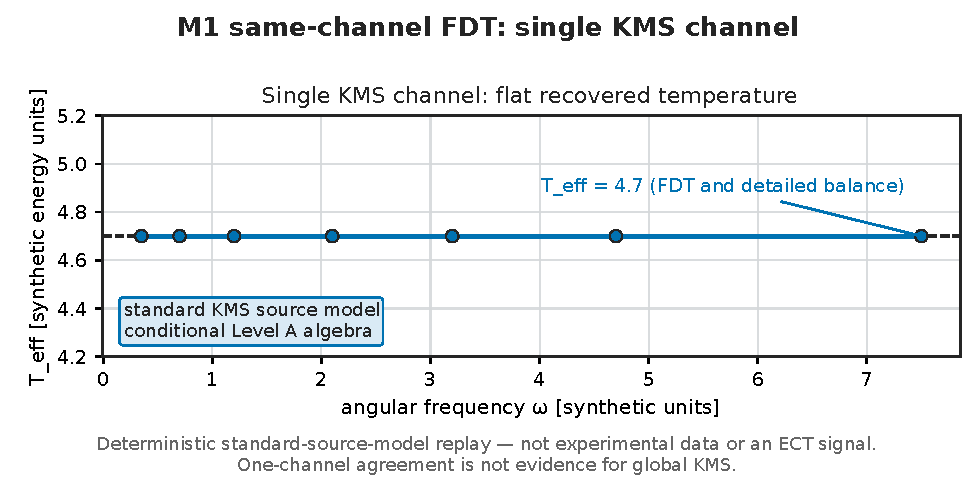
\includegraphics[width=\textwidth,height=0.76\textheight,keepaspectratio]{figures/r149/fig47_a_single_kms_channel_r149.pdf}
\caption{\textbf{M1 same-channel KMS/FDT protocol: canonical-channel
replay.}  This page shows the flat temperature recovered in one declared
canonical KMS channel.  It is a deterministic standard-source-model
algebraic check, not experimental data, an ECT signal or evidence for global
KMS thermality.  Two-bath, nonthermal-occupation and mismatched-filter
counterexamples follow on a separate full-width continuation.  A physical
test must forward-convolve the signed-frequency leakage/bin kernel, freeze or
fit $S_0$ and inter-arm gain, use an informationally complete matrix or
preregistered projections, specify generator, charges, state and preparation,
and pass causality, analyticity, Kramers--Kronig, tail, subtraction, contact
and Ward-term gates.  Current ECT evaluation remains Open because the owning
operator, vertex, state and transfer function are missing or not
identifiable.}
\label{fig:r114_pes_m1_same_channel_fdt_protocol}
\end{figure}

\begin{figure}[p]
\centering
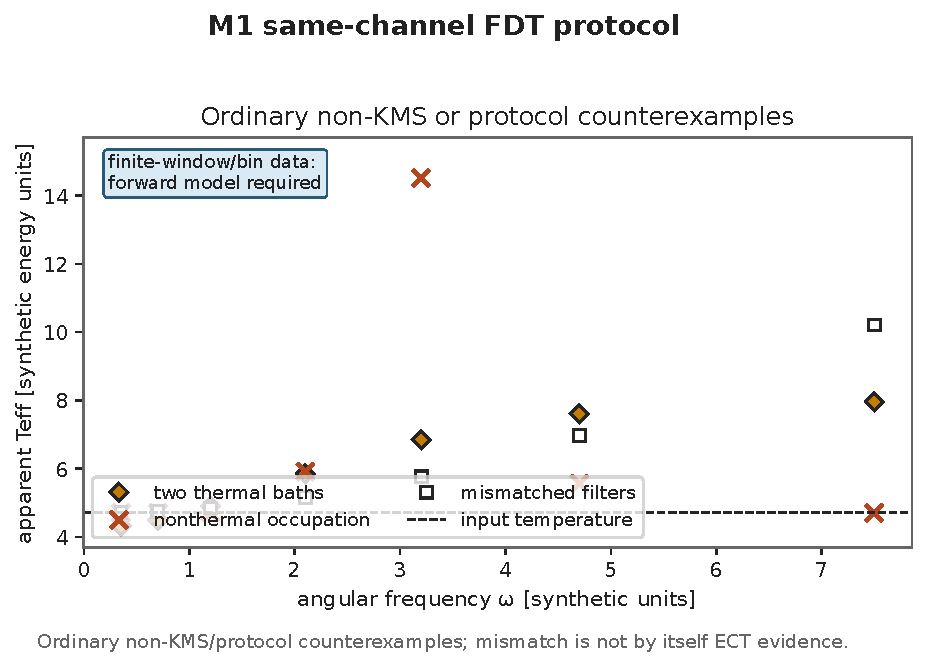
\includegraphics[width=\textwidth,height=0.76\textheight,keepaspectratio]{figures/r153/line_semantics/m1_counterexample_bins_r153.pdf}
\caption*{\textbf{Figure~\ref{fig:r114_pes_m1_same_channel_fdt_protocol}, continued.} Two-bath, nonthermal-occupation and mismatched-filter counterexamples.  The markers are independent finite-window/bin values and are not joined into a forward curve.  ECT evaluation remains Open until the physical operator, vertex, state and transfer function are identified.}
\end{figure}
\subsection{Exact cusp kernel and intrinsic resolution floor}
\label{app:AP6A-cusp}

The exact C10 cusp kernel is
\begin{equation}
\Phi(\Delta)=4\pi\left[\sqrt{4\xi_c^2+\Delta^2}-2\xi_c
-2\xi_c\ln\left(\frac{2\xi_c+\sqrt{4\xi_c^2+\Delta^2}}{4\xi_c}\right)\right].
\end{equation}
It implies the intrinsic resolution floor
\begin{equation}
  \xi_{\rm res}^{\rm intr}=4\xi_c .
\end{equation}
The large-separation logarithmic part contains the shifted logarithm
\begin{equation}
  -8\pi\xi_c\ln(\Delta/4\xi_c),
\end{equation}
which should be used when comparing finite-window fits with the asymptotic law.

\subsection{Core-profile fingerprint constants}
\label{app:AP6A-fingerprint}

For a regulated core profile $f(u)$, the approach to the universal asymptotic line slope contains a
profile-dependent fingerprint
\begin{equation}
  a_1[f]=\int_0^\infty \frac{1-f(u)}{u^2}\,du .
\end{equation}
The certified examples are
\begin{equation}
  a_1^{\rm Gauss}=\sqrt{\pi},
  \qquad
  a_1^{\rm Lorentz}=\frac{\pi}{2} .
\end{equation}
For the exponential/C10 class the approach is logarithmic rather than finite-$a_1$:
\begin{equation}
  D(R)=\frac{\xi}{R}\left[\ln\frac{R}{2\xi}+1\right]+\cdots .
\end{equation}
Thus fitted exponents below unity in finite windows should not be promoted to new physical powers until
this logarithmic law has been excluded.

\subsection{Airy-width stiffness convention}
\label{app:AP6A-Airy-stiffness}

The width-sector tilt parameter is the physical stiffness
\begin{equation}
  \kappa_b=\frac{T_{\rm line}}{2S_0} .
\end{equation}
With the transfer Hamiltonian
\begin{equation}
  H=-\frac{1}{2\kappa_b}\partial_x^2+\sigma_{\rm dec}x,
\end{equation}
the Airy ground-state scale obeys
\begin{equation}
  E_0=|a_1|\left(\frac{\sigma_{\rm dec}^2}{2\kappa_b}\right)^{1/3},
  \qquad
  \ell_w\propto (\kappa_b\sigma_{\rm dec})^{-1/3},
\end{equation}
and the coherence-window scaling is
\begin{equation}
  L_z^{\rm coh}=\frac{-\ln P_{\rm min}}{\sigma_{\rm dec}\ell_w}
  \propto \kappa_b^{1/3}\sigma_{\rm dec}^{-2/3} .
\end{equation}
A width law with $\kappa_b^{+1/3}$ is valid only after introducing a separate flexibility
$D_b=1/\kappa_b$.  The same symbol must never be used for stiffness and flexibility.

\subsection{Protocol split and matrix-kernel guard}
\label{app:AP6A-protocol-guards}

Two P6 protocol classes must not be mixed.  External or detuned monitors use the golden-rule form
\begin{equation}
  \Gamma_n^{\rm ext}=2\pi J_W(\Omega_n)|F_n(\Omega_n)|^2[1+n_{\rm eff}(\Omega_n)] .
\end{equation}
Intrinsic threshold channels instead use the dressed soft-edge pole problem and may produce a sub-edge
line plus a continuum shoulder.  In such channels a below-edge pole satisfies $\Gamma(\omega_b)=0$
within the ideal soft-edge kernel, while the spectral weight is shared between the bound line and the
continuum shoulder.

For multiple record operators the spectral object is a positive matrix, not a single scalar density:
\begin{equation}
  J_{ab}(\omega)\succeq0,
  \qquad
  |J_{ab}(\omega)|^2\le J_{aa}(\omega)J_{bb}(\omega).
\end{equation}
Scalar one-kernel closure is a further channel-selection or diagonalisation step.  This guard is required
before applying the P6-S7 triangle or the P26 over-closure test.

\subsection{Correction index local to this appendix}
\label{app:AP6A-corrections-local}

The conventions above incorporate the frozen P6 correction history: the finite-$k_z$ C8 correction, the
spatial factor-of-two correction caught by $J_{\rm spat}/J_{\rm temp}=\omega^2/c^2$, the $4\times$
reduced/canonical dictionary, the bosonic KK mirror correction, the finite-window/log artefact corrections
in P25/P18, and the P11 stiffness/flexibility transcription correction.  These are current
notes: they are part of the reproducibility conditions for the P6/PES appendices.

% ============================================================
% AP6-B inserted 2026-07-09 from derivations/pes/AP6_B_INSERT_ADAPTED_v1.tex (PES Round 30)
% ============================================================
\section{P6-B: Core spectral laws, dephasing classes, and tomography}
\label{app:AP6B-core-laws}

\paragraph{Status and scope.}
This appendix records the frozen P6/PES core spectral laws.  It uses the conventions fixed in
Appendix~\ref{app:AP6A-conventions-kernels}: Weiss spectral densities, explicit $S_0$ in thermal factors,
canonical versus reduced record kernels, and the matrix-kernel guard.  The results below are Level-B
spectral-record statements.  They organise how a certified record channel produces dephasing, induced
coefficients, tomography data, and sign constraints.  They do not prove the full PES principle from the
bare postulates, do not derive $S_0=\hbar$, and do not assert that every ECT channel is ohmic or scalar.

\subsection{L12$'$: dispersion--dimension law for the Weiss exponent}
\label{app:AP6B-L12prime}

For a channel with effective dimension $d_{\rm eff}$, dispersion $\omega\propto k^z$, vertex derivative
order $\ell$, and possible infrared matrix-element singularity exponent $\nu$, the Weiss low-frequency
spectral density
\begin{equation}
  J_W(\omega)\sim C\omega^{a_W}
\end{equation}
has exponent
\begin{equation}
  a_W=\frac{d_{\rm eff}+2\ell}{z}+2\nu-2 .
  \label{eq:AP6B-L12prime}
\end{equation}
This is a counting law for a declared record operator and channel.  It is not a rule that turns every
boundary, line, or bulk channel into an ohmic bath.  In particular, a quoted power must always specify
whether it is a bare density or a Weiss density, since the P6 convention is
$a_{\rm bare}=a_W+1$.

Equation~\eqref{eq:AP6B-L12prime} is the guard against exponent-only reasoning.  Persistent spectra are
not determined by $a_W$ alone; they are determined by the pair $(J_W,F_n)$, together with the protocol
occupation data and counterterm convention.  This is the spectral version of the pairwise record-kernel quietness
criterion: robustness is determined by the actual record difference, kernel,
and form factor, not by a slogan such as ``ohmic bath'' or by a universal
one-history PES scalar.

\subsection{L16 and L40: dephasing trichotomy}
\label{app:AP6B-L16-trichotomy}

For a stationary Gaussian record channel one may write the dephasing part in the spectral form
\begin{equation}
  \Phi(t)=\int_0^\infty d\omega\;S_{\rm rec}(\omega)
  \frac{1-\cos(\omega t)}{\omega^2},
  \label{eq:AP6B-Phi-spectral}
\end{equation}
where $S_{\rm rec}$ includes the Weiss spectral density, the relevant record-operator difference, form
factors, and the occupation/noise factor.  (The symbol $S_{\rm rec}$ is used for this
record-noise spectrum to avoid any confusion with the effective action $S_{\rm eff}$ of the
main text.)  Equivalently, for a thermal scalar channel one may absorb the
factor $\coth(S_0\omega/2T_{\rm eff})$ into $S_{\rm rec}$.  Formula~\eqref{eq:AP6B-Phi-spectral} is a
compact representation of the influence-functional class; outside the Gaussian/stationary setting the
cumulant form in Section~\ref{app:AP6B-nongaussian-quiet} is the safer definition.

If $J_W(\omega)\sim C\omega^{a_W}$ and the channel is in its vacuum occupation, the large-time behaviour
falls into the trichotomy
\begin{equation}
  \Phi(t)\sim
  \begin{cases}
    t^{1-a_W}, & a_W<1,\\
    \log t, & a_W=1,\\
    \Phi_\infty- O(t^{1-a_W}), & a_W>1 .
  \end{cases}
  \label{eq:AP6B-vacuum-trichotomy}
\end{equation}
For an actually occupied thermal channel, the additional infrared factor from
$\coth(S_0\omega/2T_{\rm eff})$ shifts the thresholds by one power:
\begin{equation}
  \Phi_T(t)\sim
  \begin{cases}
    t^{2-a_W}, & a_W<2,\\
    \log t, & a_W=2,\\
    \Phi_{T,\infty}- O(t^{2-a_W}), & a_W>2 .
  \end{cases}
  \label{eq:AP6B-thermal-trichotomy}
\end{equation}
Thus an occupied ohmic channel gives Markov-like linear growth, while a vacuum ohmic channel gives a
logarithmic dephasing law.  The word ``temperature'' in this statement refers to the occupation of the
actual record channel.  If the detailed-balance thermometer of Appendix~\ref{app:AP6A-Teff} is not constant
across the relevant band, the protocol must use $S_\pm(\omega)$ directly rather than fitting a scalar
$T_{\rm eff}$.

\subsection{L19: induced-coefficient sum rule}
\label{app:AP6B-L19-sum-rule}

The same positive spectral kernel that measures record loudness also induces the corresponding quadratic
coefficient when the record channel is integrated out.  In the Weiss convention the induced coefficient is
\begin{equation}
  \kappa_{\rm ind}=\frac{2}{\pi}\int_0^\infty \frac{J_W(\omega)}{\omega}\,d\omega .
  \label{eq:AP6B-kappa-ind}
\end{equation}
For the regulated power-law model
\begin{equation}
  J_W(\omega)=C\omega^{a_W}\exp(-\omega/\omega_c),
\end{equation}
one obtains
\begin{equation}
  \kappa_{\rm ind}=\frac{2C}{\pi}\Gamma(a_W)\omega_c^{a_W} .
  \label{eq:AP6B-kappa-ind-closed}
\end{equation}
This regulated family has the same form as $J_s(\omega)=A_s\omega^s e^{-\omega/\omega_c}$ of
Appendix~\ref{app:decoherence_apparatus}, eq.~\eqref{eq:J_s_generic}, with $C=A_s$ and $a_W=s$
\emph{when $J_s$ is read in the Weiss convention}; whether a given tabulated exponent is bare or
Weiss must be declared explicitly, per Appendix~\ref{app:AP6A-conventions-kernels}.
Consequently, once the induced coefficient and cutoff are fixed by a sector calculation, the spectral
amplitude $C$ is no longer a free loudness parameter.  In the gravitational matching route this is the
bridge from the induced coefficient to the $M_G^2$ normalisation; in the P6 record route it is the same
object appearing in dephasing and line-shift observables.  This is the first form of the one-kernel
closure later sharpened in the P6-S7/P26 appendix.

\subsection{L23, L29, L29a, and L30: non-Markov windows and finite-bath guards}
\label{app:AP6B-nongaussian-quiet}

Some P6 protocols use early-time or finite-window information rather than an asymptotic Markov rate.  A
certified example is the square-root branch
\begin{equation}
  \Phi(t)+2\sqrt{\pi}\propto t^{1/2},
  \label{eq:AP6B-sqrt-branch}
\end{equation}
which is used later as part of the guarded zero-mode/Berry detector.  This law is a channel-specific
signature, not a generic substitute for the trichotomy of Section~\ref{app:AP6B-L16-trichotomy}.

For non-Gaussian records the Gaussian variance formula must be replaced by the cumulant definition
\begin{equation}
  \Gamma=-\ln\left|\left\langle e^{iX}\right\rangle\right| .
  \label{eq:AP6B-nongaussian-cumulant}
\end{equation}
Here $X$ denotes the accumulated record variable of the channel over the protocol window.
The Gaussian expression is recovered as the leading second-cumulant approximation, but the exact
characteristic function is the object that decides whether a record is erased or superselected.

A useful corollary is the quiet-lattice rule.  If the environment records only quantised kicks on a
lattice, the dephasing functional is bounded and periodic; in particular it vanishes at integer multiples
of the environment's own quantum.  Such a bath cannot superselect states separated only by multiples of
its own kick quantum.  Winding superselection therefore requires the continuum or non-commensurate record
channel, not merely a quantised finite lattice of kicks.


For finite baths two questions must be distinguished.  Coherence is
preserved throughout a window when
\begin{equation}
  \sup_{0\le t\le T_{\rm obs}}\Phi(t)\le-\ln V_{\min},
  \label{eq:AP6B-finite-bath-coherence}
\end{equation}
whereas persistence of an already formed record requires
\begin{equation}
  \inf_{t_{\rm rec}\le t\le T_{\rm obs}}\Phi(t)\ge-\ln V_{\rm rec},
  \qquad t_{\rm rec}>0.
  \label{eq:AP6B-finite-bath-record}
\end{equation}
The infimum over $[0,T_{\rm obs}]$ is trivial because $\Phi(0)=0$.

\subsection{L31--L35b: dephasing tomography package}
\label{app:AP6B-tomography}

When $\Phi(t)$ is known over a sufficient window and has the stationary spectral representation
\eqref{eq:AP6B-Phi-spectral}, the effective spectral kernel may be reconstructed by the second-derivative
cosine inversion
\begin{equation}
  S_{\rm rec}(\omega)=\frac{2}{\pi}\int_0^\infty \Phi''(t)\cos(\omega t)\,dt .
  \label{eq:AP6B-tomography-second}
\end{equation}
This inversion supplies the basic tomography route.  Its first guard is positivity:
\begin{equation}
  S_{\rm rec}(\omega)\ge 0 .
  \label{eq:AP6B-positivity}
\end{equation}
A negative reconstructed kernel is a diagnostic of noise, window artefacts, an incorrect subtraction, or an
invalid Gaussian/stationary model.

The second guard is detailed balance.  With explicit $S_0$ convention, a thermal channel satisfies
\begin{equation}
  S_-(\omega)=\exp(-S_0\omega/T)S_+(\omega),
  \qquad \omega>0 .
  \label{eq:AP6B-detailed-balance}
\end{equation}
Failure of this relation is not automatically a failure of PES; it means that the channel is athermal,
driven, coarse-grained, or otherwise outside the scalar thermal closure.

For kernels with an asymptotic plateau $\Phi_\infty$, a derivative-free inversion is often better
conditioned:
\begin{equation}
  S_{\rm rec}(\omega)=\frac{2}{\pi}\omega^2\int_0^\infty
  \bigl[\Phi_\infty-\Phi(t)\bigr]\cos(\omega t)\,dt .
  \label{eq:AP6B-tomography-derivative-free}
\end{equation}
The frozen P6 audit found this route to be far better conditioned than direct differentiation in noisy
windows.  The methodological lesson is binding: sub-ohmic and near-ohmic classes are window-hungry, and a
finite observation time can mimic a shifted exponent unless the window law is included.

The two-regime window law is
\begin{equation}
  \text{IR bias}\sim
  \begin{cases}
    T_{\rm obs}^{-a_W}, & \omega T_{\rm obs}\lesssim 1,\\
    T_{\rm obs}^{-(a_W+1)}, & \omega T_{\rm obs}\gg 1,
  \end{cases}
  \label{eq:AP6B-window-law}
\end{equation}
up to channel-dependent prefactors.  Apparent exponents extracted from short windows must therefore be
reported together with the window, cutoff, and inversion route.

\subsection{L33 and P6-S7 preview: triangle consistency before full closure}
\label{app:AP6B-triangle-preview}

Already at the tomography level, dephasing, widths, and shifts are not independent fit parameters.  For a
fixed channel, the reconstructed $J_W$ that explains $\Phi(t)$ must also predict the golden-rule widths and
Kramers--Kronig shifts once the form factors and counterterm convention are supplied.  This is the
preliminary form of the one-kernel triangle.  The full P6-S7/P26 statement is deferred to the dedicated P6-F
appendix because the generic object is a positive spectral matrix $J_{ab}(\omega)$, not a universal scalar
bath.

\subsection{L36: sign-protection chain}
\label{app:AP6B-sign-chain}

For a certified passive record channel,
\begin{equation}
  J_W(\omega)\ge 0
\end{equation}
implies
\begin{equation}
  \kappa_{\rm ind}=\frac{2}{\pi}\int_0^\infty \frac{J_W(\omega)}{\omega}\,d\omega \ge 0 .
\end{equation}
Thus the induced contribution generated by tracing out a positive record kernel is non-negative.  This is a
sign-protection statement for the induced contribution, not a claim that every renormalised low-energy
coefficient in the full theory must be positive after all counterterms, competing sectors, and matching
conditions are included.  Whenever a negative effective coefficient is inferred, the audit question is
therefore: which subtraction, active channel, or non-passive sector has been introduced?

\subsection{Handoff to the ribbon and threshold appendices}
\label{app:AP6B-handoff}

Appendix~\ref{app:AP6A-conventions-kernels} fixes the conventions.  The present appendix records the core
spectral laws and tomography tools.  The next P6 appendices specialise these tools to the ribbon/line
sector, the certified record operators and form factors, the intrinsic threshold-protection mechanism, and
the M3 falsification protocols.  The frozen ordering is important: later claims must inherit the convention
and tomography guards above rather than redefining the bath exponent, the occupation convention, or the
counterterm convention locally.

% ============================================================
% AP6-C inserted 2026-07-09 from derivations/pes/AP6_C_INSERT_ADAPTED_v1.tex (PES Round 32)
% ============================================================
\section{P6-C: Ribbon/line sector, record classes, and form factors}
\label{app:AP6C-ribbon-line-records}

\paragraph{Status and scope.}
This appendix specialises the spectral-record machinery of Appendices~\ref{app:AP6A-conventions-kernels}
and~\ref{app:AP6B-core-laws} to the certified P6 ribbon/line sector.  The status is Level~B throughout,
except where an open input is explicitly named.  The claims below are structural record-sector statements:
they identify the line tension, endpoint guards, core and tilt inputs, Magnus fork, record operator,
record-class hierarchy, and external-monitor form-factor laws used by the later threshold and M3
appendices.  They do not derive the microscopic value of $S_0$, do not prove the colour postulate P7, and
do not turn analogue-line falsification into a falsification of the whole ECT framework.

A notational warning is needed.  Appendix~\ref{app:AP6A-zeta0} denotes the P6 Bessel-integral
line coefficient by $c_{\rm line}=1$.  This notation is used throughout the P6 appendices to avoid
collision with the orientation-stress OP-$c_1$ used elsewhere in the manuscript.  Equivalently,
\begin{equation}
  c_{\rm line}\equiv \int_0^\infty \frac{1-J_0(x)}{x^2}\,dx=1 .
  \label{eq:AP6C-line-coeff}
\end{equation}
(This is the same dimensionless number written $c_1$ in the P6 derivation files.)

\subsection{C1--C2: pair tension and ribbon area law}
\label{app:AP6C-C1-C2-tension-area}

For a pair-built winding record of transverse separation $R$ and length $L_z$, the P6 pair convention of
Appendix~\ref{app:AP6A-zeta0} gives
\begin{equation}
  \Phi_{\rm pair}(R,L_z)
  = \sigma_{\rm dec}L_zR+O(\xi_cL_z),
  \qquad
  \sigma_{\rm dec}\equiv \sigma_{\rm pair}
  =2\frac{W^2K_\theta c_\chi}{S_0} .
  \label{eq:AP6C-pair-tension}
\end{equation}
In the ledger units this is the statement that the Bessel-integral slope is $2c_{\rm line}=2$.  The
factor of two is not an optional monitor convention: all certified P6 line, width, and cusp constructions
are pair constructions.  A one-face coefficient $\sigma_{\rm face}=\sigma_{\rm pair}/2$ may be introduced only
for a genuine one-sheet object; none is currently certified in the P6 ledger.

Because the pair can be extended along $z$ without changing the transverse kernel, the line law is also a
ribbon area law,
\begin{equation}
  \Phi_{\rm ribbon}=\sigma_{\rm dec}A_{\rm ribbon}+O(\xi_cL_z),
  \qquad
  A_{\rm ribbon}=L_zR .
  \label{eq:AP6C-area-law}
\end{equation}
The excluded alternative is an isolated unscreened winding sector, whose record cost grows with the
transverse system size rather than with a finite pair separation.  Thus the finite P6 object is a bound
record pair/ribbon, not a freely isolated line charge.

\subsection{C4: endpoint mass, screening, and line-breaking guard}
\label{app:AP6C-C4-endpoint-screening}

The endpoint contribution is the core/perimeter part left after the extensive pair tension has been
separated.  Without screening, an endpoint carries an infrared-linear self-loudness and cannot be used as
a finite line-breaking defect.  With a screening length $\xi_{\rm scr}$ supplied by a specified carrier, the
certified endpoint estimate is
\begin{equation}
  M_{\rm end}=\frac{1}{2}\sigma_{\rm dec}\xi_{\rm scr} .
  \label{eq:AP6C-Mend}
\end{equation}
If breaking a ribbon changes the effective tension by $\sigma_{\rm br}>0$, the thin-wall estimates are
\begin{equation}
  R_{\rm br}=\frac{2M_{\rm end}}{\sigma_{\rm br}}
  =\frac{\sigma_{\rm dec}}{\sigma_{\rm br}}\xi_{\rm scr},
  \qquad
  B=\frac{\pi M_{\rm end}^2}{\sigma_{\rm br}}
  =\frac{\pi}{4}\frac{\sigma_{\rm dec}^2}{\sigma_{\rm br}}\xi_{\rm scr}^2 .
  \label{eq:AP6C-breaking-bounce}
\end{equation}
The thick-wall prefactor is not fixed by this argument.  The screening carrier and $\xi_{\rm scr}$ are open
sector inputs, not consequences of the line tension alone.


If an unresolved line ensemble has entropy per unit length
$s_{\rm line}=\ln\mu_{\rm step}/\xi_{\rm line}$, compare it with the
record cost per unit length.  For $\Phi=\sigma_{\rm dec}L_zR$,
\begin{equation}
  \sigma_{\rm dec}R>\frac{\ln\mu_{\rm step}}{\xi_{\rm line}},
  \qquad
  R\sim\xi_{\rm line}:\quad
  \sigma_{\rm dec}\xi_{\rm line}^2>\ln\mu_{\rm step}.
  \label{eq:AP6C-line-entropy-guard}
\end{equation}
The ensemble, core scale, and meaning of $\mu_{\rm step}$ are inputs.

\subsection{S1 and C5: core profile and tilt stiffness}
\label{app:AP6C-core-stiffness}

The reduced Ginzburg--Pitaevskii core calculation fixes the line-core profile and the dimensionless core
constant used in the ribbon sector.  In the frozen ledger the profile audit reproduces the GP value
\begin{equation}
  \frac{c_{\rm GP}}{\pi}=0.3811
  \label{eq:AP6C-GP-c0}
\end{equation}
within the quoted numerical tolerances.  (This constant is written $c_0$ in the P6 derivation files;
it is renamed $c_{\rm GP}$ here because $c_0$ denotes an entropy-capacity coefficient
elsewhere in the manuscript.)  The window-independent gradient length is
\begin{equation}
  \xi_{\rm grad}=1.477\,\xi_{\rm cond},
  \label{eq:AP6C-xi-grad}
\end{equation}
where $\xi_{\rm cond}$ is the core/healing-length parameter of this supplied
GP profile only; it is not $\xi_{\rm P3}$, an Open P4 pole length, or the bath
cutoff length unless a separate matching is supplied.  Any fitted
$\xi_{\rm eff}$ must state the finite window used to extract it.

The width-sector tilt coefficient is an independent stiffness.  In the stiffness convention fixed in
Appendix~\ref{app:AP6A-Airy-stiffness},
\begin{equation}
  \kappa_b=\frac{T_{\rm line}}{2S_0},
  \label{eq:AP6C-kappab}
\end{equation}
where $T_{\rm line}$ is the line's energetic tilt cost, including the appropriate core/log-running input for
the width scale under study.  Tension does not by itself determine the Airy width spectrum; an independent
calibration of $\kappa_b$ is required.  The loudness-gradient part of the stiffness remains an explicitly
named open input until a sector calculation supplies it.

\subsection{C6--C7: Magnus fork and the minimal ohmic branch}
\label{app:AP6C-Magnus-C7}

The minimal ribbon action inherited from the strictly second-order phase sector has the schematic form
\begin{equation}
  \frac{S_{\rm line}^{(2)}}{S_0}
  =\frac{1}{2}\int dt\,dz\,
  \left[M_\perp(\partial_t X)^2+T_{\rm line}(\partial_zX)^2\right] +\cdots .
  \label{eq:AP6C-second-order-line}
\end{equation}
It gives a linear branch $\omega\propto |k_z|$, hence dynamical exponent $z=1$.  In the P6 count this is
the minimal ohmic ribbon branch,
\begin{equation}
  n_0=0,
  \qquad
  \kappa_M^{\rm bulk}=0,
  \qquad
  z=1,
  \qquad
  a_W=1 .
  \label{eq:AP6C-minimal-ohmic}
\end{equation}
The word ``ohmic'' here is a statement about the minimal Weiss exponent of this certified branch, not a
licence to replace every subsequent protocol by a Markov bath.

A first-order Magnus/Berry term would instead have the schematic form
\begin{equation}
  \frac{S_M}{S_0}
  =\frac{i\kappa_M}{2}\int dt\,dz\,
  \left(X\partial_tY-Y\partial_tX\right),
  \qquad
  \kappa_M\propto \frac{W n_0}{S_0},
  \label{eq:AP6C-Magnus-term}
\end{equation}
and would generate a quadratic Kelvin-like branch in the infrared.  The frozen S2b verdict for the minimal
bulk ribbon is $n_0=0$; the $n_0\ne0$ route is a separate core-zero-mode/Berry branch and is tested by the
M3 zero-mode protocol, not assumed inside the minimal ribbon sector.

\subsection{C8: certified bulk record operator and soft-edge kernels}
\label{app:AP6C-C8-record-operator}

The certified bulk record operator is dictated by the pair geometry.  For a pair separated by $d$ in the
transverse plane its Fourier kernel is
\begin{equation}
  G({\bf k};d)
  =-2\pi i W\frac{k_y\cos(k_xd/2)}{k_x^2+k_y^2+k_z^2} .
  \label{eq:AP6C-Gk}
\end{equation}
Thus $|G|^2$ contains the same inverse-square kernel that appears in the C1 line-tension integral.  The
record operator is not selected from a menu after the fact: it is the particular combination of width
coordinate and time-derivative records induced by this vertex.

After the canonical C8 normalisation of Appendix~\ref{app:AP6A-C8-kernels}, the temporal and spatial
record kernels are
\begin{align}
  J_{\rm temp}^{\rm can}(\omega,k_z)
  &=\frac{\omega^2-c^2k_z^2}{16\pi\omega^3}\Theta(\omega-c|k_z|), \\
  J_{\rm spat}^{\rm can}(\omega,k_z)
  &=\frac{\omega^2-c^2k_z^2}{16\pi c^2\omega}\Theta(\omega-c|k_z|).
  \label{eq:AP6C-C8-kernels-repeat}
\end{align}
They are repeated here only to make the line-sector handoff explicit.  The ratio
$J_{\rm spat}^{\rm can}/J_{\rm temp}^{\rm can}=\omega^2/c^2$ is the preferred component-normalisation check.
The noncanonical reduced columns are $4J^{\rm can}$ and should not be mixed into the native $\Phi$-measure
line tension or cusp formulas.

\subsection{L42--L45 and C10: record classes and cusp linkage}
\label{app:AP6C-record-classes-cusp}

Record classes are organised by the infrared measure of the record difference.  In the $G$-kernel measure,
the critical exponent is
\begin{equation}
  \rho_{G,\rm crit}=1,
  \label{eq:AP6C-rhoGcrit}
\end{equation}
corresponding to $\rho_{\theta,\rm crit}=3/2$ in the certified $\Phi$-measure dictionary.  The frozen class
hierarchy is
\begin{center}
\begin{tabular*}{\textwidth}{@{\extracolsep{\fill}}lll@{}}
\toprule
record class & infrared status & interpretation \\
\midrule
endpoint & hard, power-divergent & the only hard class, $\rho=2$ \\
pair separation & finite tension & the C1/C2 pair/ribbon law \\
width difference & finite but linearly recorded & effective pair of size $|\Delta d|$ \\
translation & soft & no hard record by itself \\
\bottomrule
\end{tabular*}
\end{center}
The width-difference law, in the pair convention, is
\begin{equation}
  \frac{\Phi_{\rm width}(\Delta d)}{L_z}
  =\sigma_{\rm dec}|\Delta d|+O(\xi_c) .
  \label{eq:AP6C-width-linear}
\end{equation}
This statement is one reason the default assignment $\sigma_{\rm dec}=\sigma_{\rm pair}$ is used uniformly
throughout P6.

The exact C10 cusp kernel and the intrinsic resolution floor are given in
Appendix~\ref{app:AP6A-cusp}.  The important line-sector interpretation is that separated width sectors are
not local delta-function monitors; they are cusp-kernel objects with intrinsic floor
\begin{equation}
  \xi_{\rm res}^{\rm intr}=4\xi_c .
  \label{eq:AP6C-xires-repeat}
\end{equation}
The Gaussian monitor introduced below is a resolved-window approximation to this cusp object, not a
replacement for it at intrinsic resolution.

\subsection{C11: Gaussian width-monitor anchor}
\label{app:AP6C-C11-width-monitor}

For a Gaussian resolved width monitor with resolution $\xi_{\rm res}$, the certified anchor is
\begin{equation}
  \lambda_n^{\rm rec}=\frac{\sigma_{\rm dec}}{2\xi_{\rm res}} .
  \label{eq:AP6C-lambda-anchor}
\end{equation}
It is mode-independent at the level of the resolved Gaussian anchor.  This formula is the bridge from the
exact C10 cusp kernel to the form-factor taxonomy of the external-monitor calculation.  In intrinsic
width-sector work one should use $\xi_{\rm res}=4\xi_c$ only when the protocol really probes the intrinsic
floor; an external detector may have a larger experimental resolution.

\subsection{C12 and L46: form factors and external-monitor hierarchy}
\label{app:AP6C-C12-form-factors}

External or detuned monitors use the golden-rule form already fixed in Appendix~\ref{app:AP6A-protocol-guards},
\begin{equation}
  \Gamma_n^{\rm ext}
  =2\pi J_W(\Omega_n)|F_n(\Omega_n)|^2[1+n_{\rm eff}(\Omega_n)] .
  \label{eq:AP6C-external-width}
\end{equation}
The key C12 lesson is that the bath exponent alone does not determine the persistent spectrum.  After
dividing out the same $J_W$ and the same occupation factor, the certified form-factor hierarchy is
\begin{equation}
  |F_n|^2\sim n^0,
  \qquad
  |F_n|^2\sim n^2,
  \qquad
  |F_n|^2\sim n^2,
  \qquad
  |F_n|^2\sim n^{-2}\quad \text{on the odd-parity subsector} .
  \label{eq:AP6C-form-factor-hierarchy}
\end{equation}
The two $n^2$ entries correspond to distinct record operators with the same large-$n$ power.  They should
not be collapsed unless the underlying operator has also been identified.  Conversely, an observed width
hierarchy that does not match any certified $F_n$ class after division by $J_W$ and occupation data is a
record-operator discriminator: it challenges the proposed monitor, not the entire P6/PES framework.

\subsection{Handoff to threshold protection and M3 protocols}
\label{app:AP6C-handoff}

This appendix has established the line/ribbon object and the external-monitor form-factor hierarchy.  The
intrinsic width channel is different: its mode sits at its own soft radiation edge and must be treated by a
dressed pole plus continuum calculation.  That threshold-protection mechanism, its sum rule, and its
five-case detuning map are deferred to the next P6 appendix.  The M3 protocols then use the separation between
external C12 monitoring and intrinsic C13$'$ threshold behaviour as the primary falsifier.  Mixing the two
protocols is the main interpretive error this appendix is designed to prevent.

% ============================================================
% AP6-D inserted 2026-07-09 from derivations/pes/AP6_D_INSERT_ADAPTED_v1.tex (PES Round 34)
% Round 36: R1/R2 anti-duplication repeat markers (prose only)
% ============================================================
\section{P6-D: Intrinsic threshold protection and edge-plus-line spectra}
\label{app:AP6D-threshold-protection}

\paragraph{Status and scope.}
This appendix records the conditional C13$'$ threshold-protection mechanism of the frozen P6 ledger.  It
uses the conventions of Appendix~\ref{app:AP6A-conventions-kernels}, the core spectral laws of
Appendix~\ref{app:AP6B-core-laws}, and the certified line/width record operator of
Appendix~\ref{app:AP6C-ribbon-line-records}.  The status is Level~B conditional.  The result is a
statement about an intrinsic width-channel self-record sitting at its own soft radiation edge.  It is not a
generic statement about every external monitor, every oscillator coupled to a bath, or every line in the
analogue laboratory.  In particular, the external-monitor golden-rule hierarchy remains the C12 result of
Appendix~\ref{app:AP6C-C12-form-factors}; the present appendix treats the intrinsic dressed-pole problem.

The robustness claim below is the vanishing of the width for a pole below the edge, together with the
line-plus-shoulder spectral form and the associated sum rule.  The absolute binding energy below the edge is
not invariant until the counterterm and detuning convention have been declared.

\subsection{Soft edge inherited from C8}
\label{app:AP6D-soft-edge}

For fixed longitudinal momentum $k_z$, the certified C8 kernels have the threshold
\begin{equation}
  E\equiv E_{\rm edge}=c|k_z|,
\end{equation}
and vanish below it.  Near the edge, with $\epsilon=\omega-E>0$, Appendix~\ref{app:AP6A-C8-kernels} gives
\begin{align}
  J_{\rm temp}^{\rm can}(\omega,k_z)
  &=\frac{\epsilon}{8\pi E^2}+O(\epsilon^2), \\
  J_{\rm spat}^{\rm can}(\omega,k_z)
  &=\frac{\epsilon}{8\pi c^2}+O(\epsilon^2).
  \label{eq:AP6D-C8-edge-onset}
\end{align}
Thus the intrinsic width channel sees a soft linear continuum onset rather
than a hard threshold singularity.  For the threshold analysis it is useful
to write the effective edge
kernel in the form
\begin{equation}
  J_{\rm edge}(\omega)
  =g^2A_E(\omega-E)\Theta(\omega-E)f_{\rm UV}(\omega),
  \qquad
  A_E>0,
  \qquad
  f_{\rm UV}(E)=1,
  \label{eq:AP6D-soft-edge-model}
\end{equation}
where $g$ is the channel amplitude and $A_E$ includes the selected temporal/spatial component, source
normalisation, and any declared projection.  Equation~\eqref{eq:AP6D-soft-edge-model} is a local threshold
model, not a replacement for the full C8 kernel away from the edge.

\subsection{Dressed intrinsic response and bosonic mirror dispersion}
\label{app:AP6D-dressed-response}

The intrinsic width mode is represented by the retarded dressed response
\begin{equation}
  G_R(z)=\frac{1}{D(z)},
  \qquad
  D(z)=z^2-\Omega_0^2+\Sigma_R(z)-\delta_{ct}.
  \label{eq:AP6D-dressed-response}
\end{equation}
Here $\Omega_0$ is the frequency in the declared bare or calibrated convention, $\delta_{ct}$ is the
subtraction convention, and $\Sigma_R$ is computed with the bosonic mirror kernel of
Appendix~\ref{app:AP6A-KK-counterterm}.  Recalling that convention, with a positive continuum width above
the edge, the real part is
\begin{equation}
  \Sigma'(\omega)=\frac{2}{\pi}\,\mathcal{P}\int_E^\infty
  \frac{\omega'\Sigma''(\omega')}{\omega'^2-\omega^2}\,d\omega' .
  \label{eq:AP6D-bosonic-KK}
\end{equation}
The one-sided kernel $1/(\omega'-\omega)$ is not used in the frozen P6 branch.  It fails the oscillator
sum-rule audit and is included in the correction history rather than in the certified convention.

A real pole below the edge satisfies
\begin{equation}
  D(\omega_b)=0,
  \qquad
  \omega_b<E.
  \label{eq:AP6D-subedge-pole}
\end{equation}
Because $J_{\rm edge}(\omega_b)=0$, the intrinsic continuum gives
\begin{equation}
  \Gamma(\omega_b)=0
  \label{eq:AP6D-zero-width}
\end{equation}
before any external readout convolution or environmental leakage is added.  This is the core of threshold
protection.  It should not be confused with a weak but finite Lorentzian width above the edge.

\subsection{\texorpdfstring{C13$'$}{C13-prime}: the conditional threshold-protection statement}
\label{app:AP6D-C13prime}

In the self-consistent intrinsic width channel, the undressed width mode is edge-aligned in the ideal
minimal geometry,
\begin{equation}
  \Omega_0=E_{\rm edge},
  \label{eq:AP6D-edge-alignment}
\end{equation}
and is dressed by its own soft edge.  In a bare-edge convention this produces a subedge pole,
\begin{equation}
  \omega_b<E_{\rm edge},
  \qquad
  E_{\rm edge}-\omega_b=O(g^2),
  \qquad
  \Gamma(\omega_b)=0,
  \label{eq:AP6D-binding-scaling}
\end{equation}
with a soft continuum shoulder above the edge.  The $O(g^2)$ statement is made with $g$ the channel
amplitude; if the scan variable is already $g^2$, the fitted exponent is unity.

The intrinsic spectral form is therefore
\begin{equation}
  \rho_{\rm intr}(\omega)
  =\frac{Z_b}{2\omega_b}\delta(\omega-\omega_b)
   +\rho_{\rm cont}(\omega)\Theta(\omega-E_{\rm edge}) .
  \label{eq:AP6D-edge-plus-line}
\end{equation}
This is not the C12 external-monitor spectrum.  The C12 form is recovered only when an external or detuned
monitor reads the width family through the golden-rule expression in
Appendix~\ref{app:AP6C-C12-form-factors}.  The primary M3 discriminator is precisely this two-protocol
contrast.

\subsection{Spectral-weight sum rule}
\label{app:AP6D-sum-rule}

The subedge line and the continuum shoulder are not independent fit components.  In the oscillator
normalisation used in the P6 audits they obey
\begin{equation}
  Z_b+\int_E^\infty 2\omega\rho_{\rm cont}(\omega)\,d\omega=1.
  \label{eq:AP6D-sum-rule}
\end{equation}
Equivalently, $Z_b$ is the oscillator-normalised residue of $G_R$ at the subedge pole,
\begin{equation}
  Z_b=\frac{2\omega_b}{D'(\omega_b)}
  =\left[1+\frac{1}{2\omega_b}\frac{d}{d\omega}
    \bigl(\Sigma'(\omega)-\delta_{ct}\bigr)\bigg|_{\omega=\omega_b}\right]^{-1},
  \label{eq:AP6D-residue}
\end{equation}
when the counterterm is frequency-independent.  If a different response normalisation is used, the sum
rule must be transformed with it; the invariant content is that line weight lost from $Z_b$ appears in the
same channel's continuum shoulder.  This guard eliminates the false positive in which an unrelated trapped
mode is fitted as a protected intrinsic line.

\subsection{Five-case detuning and counterterm map}
\label{app:AP6D-five-case-map}

The detuning is
\begin{equation}
  \Delta=\Omega_0-E_{\rm edge}.
  \label{eq:AP6D-detuning}
\end{equation}
Throughout this appendix $\Delta$ denotes the edge detuning in Eq.~\eqref{eq:AP6D-detuning};
the transverse-separation variable used in the cusp-kernel discussion of
Appendix~\ref{app:AP6A-cusp} is local to that discussion and is not used below.
The following cases define the frozen C13$'$ map.

\par\Needspace*{20\baselineskip}
\begin{longtable}{@{}L{0.17\textwidth}L{0.38\textwidth}L{0.39\textwidth}@{}}
\toprule
case & condition & outcome and guard \\
\midrule
\endfirsthead
\toprule
case & condition & outcome and guard \\
\midrule
\endhead
\bottomrule
\endfoot
\bottomrule
\endlastfoot
bare edge & $\Delta=0$ with a declared bare-edge convention & A subedge pole detaches with binding $O(g^2)$ and zero intrinsic width.  The numerical binding is convention-dependent. \\
physical edge & $\delta_{ct}$ chosen so that the $g\to0$ physical edge is fixed & The pole may sit at the edge in the calibrated convention, but any pole below the edge still has $\Gamma=0$.  Do not quote an absolute detachment without the subtraction convention. \\
positive detuning & $\Delta>0$ & Below a critical coupling the mode is an over-edge resonance.  Above it the pole rebinds below the edge.  The transition defines P24. \\
negative detuning & $\Delta<0$ & The pole is already subedge in the calibrated limit; protection is then kinematic rather than a nontrivial rebinding. \\
finite system or finite readout & edge levels, disorder, external leakage, finite $T_{\rm obs}$ & The mathematical pole is observed with residual width set by the largest non-intrinsic broadening scale in Eq.~\eqref{eq:AP6D-observed-width}. \\
\end{longtable}

For the positive-detuning branch, the soft-edge model gives the leading scaling
\begin{equation}
  g^2_{\rm crit}(\Delta)=\frac{\Delta}{\chi_E}+O(\Delta^2),
  \qquad
  \chi_E>0,
  \label{eq:AP6D-gcrit-linear}
\end{equation}
Here $g^2_{\rm crit}$ is the critical channel amplitude of this detuning map; it is unrelated to
the alignment coupling $g_{\rm crit}$ of the electroweak sector of the main text.  It follows that
\begin{equation}
  \frac{d\log g^2_{\rm crit}}{d\log\Delta}=1+O(\Delta).
  \label{eq:AP6D-P24-slope}
\end{equation}
The coefficient $\chi_E$ is not universal: it depends on the edge normalisation, cutoff, projection, and
counterterm convention.  The unit exponent is the P24 prediction.  If the measured continuum-onset exponent
is not the C8 soft-edge exponent, the P24 exponent must be rederived before interpreting a failure as a
failure of threshold protection.

\subsection{Finite-resolution and observed width}
\label{app:AP6D-finite-resolution}


Below-edge zero width is an intrinsic-channel statement.  The measured line
shape is a convolution of intrinsic, external, finite-size, thermal,
disorder, finite-window, and instrumental responses.  Independent
Lorentzian rates add, Gaussian variances add in quadrature, and mixed
broadening is generally Voigt-like.  Only as a conservative scale estimate,
\begin{equation}
  \Gamma_{\rm obs}^{({\rm scale})}\sim
  \max(\Gamma_{\rm ext},\Gamma_{L_z},\Gamma_T,\Gamma_{\rm disorder},
  T_{\rm obs}^{-1},\delta\omega_{\rm res}),
  \label{eq:AP6D-observed-width}
\end{equation}
while a quantitative fit must convolve the declared response functions.

Resolving the line as a subedge line rather than as an edge shoulder requires
\begin{equation}
  E_{\rm edge}-\omega_b \gtrsim 3\delta\omega_{\rm res},
  \label{eq:AP6D-line-resolution}
\end{equation}
while resolving the shoulder as a continuum rather than as a few finite-size levels requires the opposite
hierarchy for the edge-level spacing,
\begin{equation}
  \delta\omega_{\rm level}\ll \delta\omega_{\rm res} .
  \label{eq:AP6D-shoulder-resolution}
\end{equation}
Both inequalities must be stated in any proposed M3 implementation.  A failure caused by finite resolution
is a protocol failure, not a falsification of C13$'$.

\subsection{P23/P24 two-protocol falsifier}
\label{app:AP6D-P23-P24}

The intrinsic protocol fits the spectrum, after convolution with the experimental resolution kernel
$R_{\rm res}$, as
\begin{equation}
  \rho_{\rm intr}^{\rm obs}(\omega)
  =\left[\frac{Z_b}{2\omega_b}\delta(\omega-\omega_b)+\rho_{\rm cont}(\omega)\Theta(\omega-E)\right]
   \ast R_{\rm res}(\omega),
  \label{eq:AP6D-intrinsic-observed}
\end{equation}
with $\omega_b<E$, $\Gamma(\omega_b)=0$ before convolution, and the sum rule
\eqref{eq:AP6D-sum-rule}.  The external protocol, recalling the C12 monitor law of
Appendix~\ref{app:AP6C-C12-form-factors}, fits the same width-mode family with
\begin{equation}
  \Gamma_n^{\rm ext}=2\pi J_W(\Omega_n)|F_n(\Omega_n)|^2[1+n_{\rm eff}(\Omega_n)] .
  \label{eq:AP6D-external-repeat}
\end{equation}
After division by the same $J_W$ and occupation data, the external hierarchy must reduce to the C12
form-factor classes of Appendix~\ref{app:AP6C-C12-form-factors}.  P23 is the contrast between these two
protocols.  P24 is the positive-detuning transition
\begin{equation}
  \text{over-edge resonance}
  \quad\longrightarrow\quad
  \text{subedge line plus soft shoulder},
  \qquad
  g^2_{\rm crit}(\Delta)\propto\Delta .
  \label{eq:AP6D-P24-transition}
\end{equation}

The falsification hierarchy is deliberately local.  A failed P23/P24 implementation first challenges the
proposed C8/C13$'$ intrinsic record operator, then the edge-alignment assumption, then the soft-edge
threshold mechanism, and only after the protocol guards are controlled does it challenge the wider P6/PES
spectral-record framework.  It does not by itself falsify all of ECT.

\paragraph{External band-edge sanity checks.}
The line-plus-continuum component of the C13$'$ package is the same
open-system structure that appears in standard band-edge reservoir physics:
a bound component below or outside a continuum edge, together with
non-Markovian continuum decay.  Existing superconducting-metamaterial and
matter-wave experiments provide external consistency checks on the P6
conventions.  In Mirhosseini et al.~\cite{Mirhosseini2018}, the same
engineered reservoir accounts for both the lifetime anomaly and the Lamb-shift
anomaly of a transmon near a metamaterial band edge; this is a
source-model-level pass of the one-reservoir width/shift pattern, not yet an
independent quantitative P26 residual test.  In the matter-wave experiments of
Krinner et al.~\cite{Krinner2018} and Stewart et al.~\cite{Stewart2020}, bound
states and non-Markovian continuum dynamics realise the C13$'$ line-plus-continuum
pattern in the singular one-dimensional edge class.  In all of these published
platforms the accessible edge is of van-Hove type, effectively $m=-1/2$, or
more singular, so the P24 soft-edge prediction $g_{\rm crit}^2\propto\Delta$
is not tested there.  These comparisons show that the frozen P6 conventions
reproduce known band-edge open-system physics; they are not claimed as evidence
that PES is superior to standard quantum open-system theory.  A direct P24 test
requires an engineered convergent one-sided reservoir, for example a gapped
Ohmic edge $J(\omega)=\eta(\omega-E)\Theta(\omega-E)$.

\subsection{Operational guards}
\label{app:AP6D-operational-guards}

The following guards must accompany any use of C13$'$ or P23/P24.
\begin{enumerate}
  \item \emph{Backaction guard.}  Vary readout strength and extrapolate to the weak-reading intercept; a
  strong readout can turn an intrinsic channel into an external C12 monitor.
  \item \emph{Trapped-mode guard.}  A subedge line without transfer of weight to the soft shoulder is not a
  C13$'$ line.  The sum rule~\eqref{eq:AP6D-sum-rule} is mandatory.
  \item \emph{Detuning guard.}  Calibrate $\Delta$ by a declared $g\to0$ or counterterm-subtracted
  procedure before fitting $g^2_{\rm crit}(\Delta)$.
  \item \emph{Edge-exponent guard.}  Measure the continuum-onset exponent independently.  The P24 unit
  exponent assumes the C8 soft linear edge.
  \item \emph{Finite-size guard.}  Check Eqs.~\eqref{eq:AP6D-line-resolution} and
  \eqref{eq:AP6D-shoulder-resolution} before interpreting line/shoulder visibility.
  \item \emph{Matrix-channel guard.}  If intrinsic and external readouts project different eigenchannels of
  $J^W_{ab}$, scalar closure can fail without falsifying the matrix P6-S7 framework.
\end{enumerate}
These guards are operational rather than decorative: they determine whether a laboratory outcome is a
C13$'$ result, a record-operator failure, a protocol failure, or an ambiguous mixed-channel measurement.

\subsection{Handoff}
\label{app:AP6D-handoff}

Appendix~\ref{app:AP6C-ribbon-line-records} established the certified external-monitor hierarchy.  The
present appendix establishes the intrinsic edge-plus-line mechanism and its detuning transition.
Appendix~\ref{app:AP6E-width-observable-interface} supplies the width-sector observable interface,
Appendix~\ref{app:AP6F-matrix-triangle-P26} supplies the P6-S7/P26 over-closure test, and
Appendix~\ref{app:AP6G-M3-operational-protocols} assembles M3-1, M3-2, and M3-3 as explicit
falsification protocols.  The handoff rule is simple: C12 governs external or detuned monitoring, C13$'$
governs the intrinsic self-channel, and a calculation that mixes the two without stating the protocol is not
a valid P6 prediction.

% ============================================================
% AP6-E inserted 2026-07-09 from derivations/pes/AP6_E_INSERT_ADAPTED_v1.tex (PES Round 37)
% ============================================================
\section{P6-E: Width-sector observable interface and M3-3 over-closure inputs}
\label{app:AP6E-width-observable-interface}

\paragraph{Status and scope.}
This appendix is an interface layer.  It uses the convention dictionary of
Appendix~\ref{app:AP6A-conventions-kernels}, the line/width record operators of
Appendix~\ref{app:AP6C-ribbon-line-records}, and the intrinsic threshold-protection test of
Appendix~\ref{app:AP6D-threshold-protection}.  It does not rederive the pair normalisation
$\zeta_0^{\rm pair}=2$, the C10 cusp kernel, the P25/P25$'$ fingerprint constants, the Airy transfer
Hamiltonian, or C13$'$ threshold protection.  Its role is to state the observable chain used by the P6-S7/P26 over-closure test of
Appendix~\ref{app:AP6F-matrix-triangle-P26} and by the M3 protocols of
Appendix~\ref{app:AP6G-M3-operational-protocols}, without duplicating the derivations already owned by
Appendices~\ref{app:AP6A-conventions-kernels}--\ref{app:AP6D-threshold-protection}.

\subsection{Observable chain}
\label{app:AP6E-observable-chain}

The width-sector chain is
\begin{equation}
\begin{gathered}
  \text{static core-profile fit}
  \longrightarrow \widehat{\xi}_c
  \longrightarrow \widehat{\xi}_{\rm res}=4\widehat{\xi}_c
  \longrightarrow \lambda_n^{\rm rec}
  \\
  \longrightarrow
  \left(\widehat{\ell}_w,\widehat{E}_0,\widehat{L}_z^{\rm coh}\right)
  \longrightarrow
  \text{C13$'$ protection check}.
\end{gathered}
\label{eq:AP6E-observable-chain}
\end{equation}
The first arrow uses the P25/P25$'$ profile fingerprints of Appendix~\ref{app:AP6A-fingerprint}.  The
second uses the intrinsic resolution floor of Appendix~\ref{app:AP6A-cusp}.  The monitor anchor
$\lambda_n^{\rm rec}$ is the Gaussian record coefficient of Appendix~\ref{app:AP6C-C11-width-monitor}.
The Airy quantities use the stiffness convention of Appendix~\ref{app:AP6A-Airy-stiffness}.  The final
arrow is not optional: a width distribution is a persistent quantum width candidate only if the intrinsic
line also passes the C13$'$ edge-plus-line test of Appendix~\ref{app:AP6D-threshold-protection}.

\subsection{Independent tilt calibration}
\label{app:AP6E-tilt-calibration}

The width stiffness must be calibrated independently from a tilt-cost measurement.  For a small imposed
tilt $v$, the operational calibration is
\begin{equation}
  \frac{\Delta\Phi_{\rm tilt}(v)}{L_z}
  =\frac{\widehat{\kappa}_b}{2}v^2+O(v^4).
  \label{eq:AP6E-tilt-calibration}
\end{equation}
The hat emphasises that this is a measured stiffness.  It must not be inferred from the Airy width fit
itself and then reused to claim the $\kappa_b^{-1/3}$ width scaling.  That circular procedure would make
the stiffness exponent tautological even for a false width model.  The Airy-width test is therefore
meaningful only after Eq.~\eqref{eq:AP6E-tilt-calibration}, or an equivalent independent stiffness
calibration, has fixed $\widehat{\kappa}_b$.

\subsection{Resolution and deconvolution guard}
\label{app:AP6E-resolution-deconvolution}

Let $P_{\rm obs}(x)$ be the measured width distribution and $R_{\rm res}(x)$ the independently measured
instrumental resolution.  The model comparison should use
\begin{equation}
  P_{\rm obs}(x)=P_{\rm wid}(x)\ast R_{\rm res}(x),
  \label{eq:AP6E-resolution-convolution}
\end{equation}
not an unsmeared Airy profile.  For an approximately Gaussian resolution with variance
$\sigma_{\rm res}^2$, the variance-level deconvolution is
\begin{equation}
  m_{2,{\rm dec}}=m_{2,{\rm obs}}-\sigma_{\rm res}^2 .
  \label{eq:AP6E-variance-deconvolution}
\end{equation}
This formula is only a variance diagnostic; the full profile comparison should convolve the candidate
distribution with the measured $R_{\rm res}$.  The certified operational requirement from the frozen P6
M3-3 audit is
\begin{equation}
  \sigma_{\rm res}\lesssim 0.3\,\widehat{\ell}_w .
  \label{eq:AP6E-resolution-bound}
\end{equation}
Above this scale, deconvolution errors can mimic or erase the Airy tail diagnostics.
(In the frozen P6 audit ledger this bound is recorded as
$\sigma_{\rm res}\lesssim0.3\,\ell_A$, where $\ell_A$ is the ledger name for the Airy width
scale denoted $\ell_w$ in Appendix~\ref{app:AP6A-Airy-stiffness}.)

\subsection{Shape collapse and non-circular Airy test}
\label{app:AP6E-shape-collapse}

Using the independent $\widehat{\kappa}_b$ and the already fixed $\sigma_{\rm dec}$ convention, the Airy
prediction gives a width scale $\widehat{\ell}_w$ by Appendix~\ref{app:AP6A-Airy-stiffness}.  The
shape-collapse test compares
\begin{equation}
  \widehat{\ell}_w\,P_{\rm wid}(\widehat{\ell}_w u)
  \quad\text{against the universal half-line Airy profile in }u .
  \label{eq:AP6E-shape-collapse}
\end{equation}
The scale collapse is not a substitute for the exponent test: both the profile shape and the independent
scalings with $\sigma_{\rm dec}$ and $\widehat{\kappa}_b$ must be checked.  Conversely, a cube-root
scaling alone is not sufficient evidence for a persistent quantum width, because thermal broadening,
trapping, or resolution convolution can generate similar apparent powers over finite windows.

\subsection{C13$'$ protection check}
\label{app:AP6E-C13-check}

The width-sector observable chain must be paired with the intrinsic threshold test.  The required C13$'$
signature is the package
\begin{equation}
  \text{subedge line}
  +\text{ soft continuum shoulder}
  +\text{ same-channel sum rule}
  +\text{ P24 detuning transition}.
  \label{eq:AP6E-C13-package}
\end{equation}
Here the sum rule and detuning map are those of Appendix~\ref{app:AP6D-sum-rule} and
Appendix~\ref{app:AP6D-five-case-map}.  A width profile without this intrinsic protection check should be
reported as a width-profile observation, not as a persistent Airy-width record.

\subsection{M3-3 decision table}
\label{app:AP6E-M3-3-decision-table}

The following table is an operational interface for M3-3 in
Appendix~\ref{app:AP6G-M3-operational-protocols}.  It is not a new
derivation of the Airy or fingerprint laws.

\begin{longtable}{@{}L{0.30\textwidth}L{0.30\textwidth}L{0.32\textwidth}@{}}
\caption{Operational M3-3 width, fingerprint, and intrinsic-protection
decision interface.}
\label{tab:AP6E-M3-3-decision}\\
\toprule
Observation & Required companion check & Interpretation \\
\midrule
\endfirsthead
\toprule
Observation & Required companion check & Interpretation \\
\midrule
\endhead
\bottomrule
\endfoot
\bottomrule
\endlastfoot
Fingerprint fit gives stable $\widehat{\xi}_c$ & Consistent $\widehat{\xi}_{\rm res}=4\widehat{\xi}_c$ in the record monitor & Core profile scale is usable as width-sector input \\
Airy-like width profile & Independent tilt calibration from Eq.~\eqref{eq:AP6E-tilt-calibration} & Non-circular candidate for quantum width \\
Apparent cube-root scaling only & Resolution bound Eq.~\eqref{eq:AP6E-resolution-bound} and full convolution test & Ambiguous unless deconvolution and shape collapse pass \\
Width profile passes, C13$'$ package fails & Threshold package Eq.~\eqref{eq:AP6E-C13-package} & Width is not yet a persistent intrinsic record \\
All checks pass & Same-channel P23/P24 contrast in Appendix~\ref{app:AP6D-P23-P24} & Candidate M3-3 success case \\
\end{longtable}

\subsection{Handoff}
\label{app:AP6E-handoff}

Appendix~\ref{app:AP6B-triangle-preview} previews the idea that dephasing, shifts, and widths should
over-close when they are projections of the same positive record kernel, and
Appendix~\ref{app:AP6F-matrix-triangle-P26} gives the full P6-S7/P26 test.  The present appendix supplies
the width-sector observable inputs for that over-closure test and for the M3-3 protocol of
Appendix~\ref{app:AP6G-M3-operational-protocols}.  The protocol should call the quantities defined here
rather than repeating the normalisation, fingerprint, and Airy derivations of
Appendix~\ref{app:AP6A-conventions-kernels}.

% ============================================================
% AP6-F inserted 2026-07-09 from derivations/pes/AP6_F_INSERT_ADAPTED_v1.tex (PES Round 39)
% + R3 micro-patch: bare S7 -> P6-S7 across BI-BM (7 loci)
% ============================================================
\section{P6-F: Matrix one-kernel triangle and P26 over-closure}
\label{app:AP6F-matrix-triangle-P26}

\paragraph{Status and scope.}
This appendix gives the full P6-S7/P26 closure test.  The label P6-S7 refers to the spectral-record
milestone of the frozen P6 ledger, not to the foundational S7 admissibility postulate of the main
axiomatic list.  The preview in Appendix~\ref{app:AP6B-triangle-preview} is upgraded here to an
operational over-closure test.  The generic object is a positive record spectral matrix; a scalar
one-kernel triangle is valid only after a channel-selection or diagonalisation step.

The synthetic replay is Level~A only inside its supplied identifiable
two-parameter kernel family.  P26 as a preregistered cross-arm protocol is
Level~B.  A model-independent reconstruction of an arbitrary continuum from a
finite set of widths is not established, and a physical ECT implementation
remains Open until its record operator, state, form factors, kernel family and
calibrated measurement map are supplied.

This appendix does not rederive the dephasing classes of Appendix~\ref{app:AP6B-L16-trichotomy}, the
C12 form-factor hierarchy of Appendix~\ref{app:AP6C-C12-form-factors}, the C13$'$ threshold mechanism of
Appendix~\ref{app:AP6D-threshold-protection}, or the width-observable chain of
Appendix~\ref{app:AP6E-width-observable-interface}.  It uses those results as inputs.

\subsection{Matrix record kernel}
\label{app:AP6F-matrix-kernel}

For a set of record operators labelled by $a,b$, the P6 record environment is represented by a Weiss
spectral matrix
\begin{equation}
  J^W_{ab}(\omega)\succeq0,\qquad \omega>0 .
  \label{eq:AP6F-positive-matrix-kernel}
\end{equation}
Recalling the matrix guard of Appendix~\ref{app:AP6A-protocol-guards}, positivity implies the pointwise
Cauchy--Schwarz test
\begin{equation}
  |J^W_{ab}(\omega)|^2\le J^W_{aa}(\omega)J^W_{bb}(\omega).
  \label{eq:AP6F-CS-test}
\end{equation}
A violation of Eq.~\eqref{eq:AP6F-CS-test} is not a subtle model-selection issue: it means the proposed
cross-channel spectral data cannot be a passive positive record kernel in the declared convention.

At a fixed frequency one may diagonalise
\begin{equation}
  J^W_{ab}(\omega)=\sum_r j_r(\omega)e_a^{(r)}(\omega)e_b^{(r)}(\omega)^*,
  \qquad j_r(\omega)\ge0 .
  \label{eq:AP6F-frequency-diagonalisation}
\end{equation}
A scalar triangle is therefore a selected-channel statement.  It is justified when the protocol excites a
single eigenchannel $r$, or when a declared projection $\Pi_r$ is stable over the frequency window being
tested.  If the eigenvectors $e^{(r)}(\omega)$ rotate significantly across the window, scalar closure can
fail even though the matrix P6-S7 statement remains viable.

\subsection{P6-S7 triangle for one selected channel}
\label{app:AP6F-scalar-triangle}

For a selected channel $r$, define the projected density
\begin{equation}
  J^W_r(\omega)=\Pi_r^\dagger J^W(\omega)\Pi_r .
  \label{eq:AP6F-projected-density}
\end{equation}
The P6-S7 triangle is the statement that, once the protocol data are declared, the three observed
quantities are not independent fits:
\begin{equation}
  J^W_r(\omega)
  \quad\Longrightarrow\quad
  \left\{
  \Phi_r(t),\ \Gamma_{n,r},\ \delta\Omega_{n,r}
  \right\}.
  \label{eq:AP6F-triangle-map}
\end{equation}
The dephasing arm uses the spectral representation of Appendix~\ref{app:AP6B-L16-trichotomy}.  The width
arm uses the C12 external-monitor form factors of Appendix~\ref{app:AP6C-C12-form-factors}, or the
intrinsic threshold objects of Appendix~\ref{app:AP6D-threshold-protection} when the channel is a C13$'$
self-channel.  The shift arm uses the bosonic mirror convention of Appendix~\ref{app:AP6D-dressed-response}
and the counterterm convention declared for the protocol.

For an external monitor, the width arm is
\begin{equation}
  \Gamma_{n,r}^{\rm ext}
  =2\pi J^W_r(\Omega_n)|F_{n,r}(\Omega_n)|^2[1+n_{\rm eff}(\Omega_n)] .
  \label{eq:AP6F-external-width-arm}
\end{equation}
The corresponding counterterm-relative leading shift is obtained from the same projected kernel through
the bosonic mirror map,
\begin{equation}
  \delta\Omega_{n,r}
  =
  -\frac{\Sigma'_{n,r}(\Omega_n)-\delta_{ct,n}}{2\Omega_n}
  +O(\Sigma^2),
  \label{eq:AP6F-shift-arm}
\end{equation}
where the sign follows the dressed-response convention
$D(z)=z^2-\Omega_n^2+\Sigma_R(z)-\delta_{ct,n}$ used in Appendix~\ref{app:AP6D-dressed-response}.  If a
different subtraction convention is used in a concrete protocol, Eq.~\eqref{eq:AP6F-shift-arm} must be
translated before comparison with data.

\subsection{P26 reconstruction loop}
\label{app:AP6F-P26-loop}

P26 is an over-closure loop that fits or identifies a preregistered kernel family from one arm, when that
family is identifiable, and tests it against the other two.  In an external C12 protocol the width arm first
supplies sampled projected values:
\begin{equation}
  \widehat J^W_r(\Omega_n)
  =
  \frac{\Gamma_{n,r}^{\rm ext}}
       {2\pi |F_{n,r}(\Omega_n)|^2[1+n_{\rm eff}(\Omega_n)]}.
  \label{eq:AP6F-width-reconstruction}
\end{equation}
A finite set of widths does not determine the continuum kernel between the
$\Omega_n$, its unmeasured bands, ultraviolet tail, subtraction, or counterterm.
A positive interpolation or kernel family is therefore an additional,
preregistered model input.  Conditional on its identifiability, the fitted
$\widehat J^W_r(\omega)$ then predicts
\begin{equation}
  \widehat\Phi_r(t_i)
  =
  \int_0^\infty d\omega\,
  \widehat S_{{\rm rec},r}(\omega)
  \frac{1-\cos\omega t_i}{\omega^2},
  \label{eq:AP6F-predicted-dephasing}
\end{equation}
using the same record-spectrum convention as Appendix~\ref{app:AP6B-L16-trichotomy}, and predicts
\begin{equation}
  \widehat{\delta\Omega}_{n,r}
  =
  -\frac{\widehat\Sigma'_{n,r}(\Omega_n)-\delta_{ct,n}}{2\Omega_n}.
  \label{eq:AP6F-predicted-shift}
\end{equation}
The hats mark predictions from the same fitted/identified kernel family, not
independent fits and not a model-independent reconstruction of an arbitrary
continuum spectrum.  The uncertainties and covariance of
$F_{n,r}(\Omega_n)$ and $n_{\rm eff}(\Omega_n)$ must be propagated through
Eq.~\eqref{eq:AP6F-width-reconstruction}; divisions by a poorly known or
near-zero form factor are not informative.  If the family has parameters
$\boldsymbol\theta$, the sampled forward map
$\boldsymbol\theta\mapsto\{\Gamma_{n,r}^{\rm ext}\}_n$ must be injective on
the preregistered domain before the width arm is called \emph{globally}
identifiable.  Full Jacobian rank at a point supports only local
identifiability in a neighbourhood of that point and must not be reported as
global reconstruction.

The over-closure residuals may be reported as
\begin{equation}
  R^{\rm oc}_\Phi
  =
  \max_i
  \left|
  \frac{\Phi_r^{\rm obs}(t_i)-\widehat\Phi_r(t_i)}
       {\sigma_{\Phi,i}}
  \right|,
  \qquad
  R^{\rm oc}_\Omega
  =
  \max_n
  \left|
  \frac{\delta\Omega_{n,r}^{\rm obs}-\widehat{\delta\Omega}_{n,r}}
       {\sigma_{\Omega,n}}
  \right|.
  \label{eq:AP6F-overclosure-residuals}
\end{equation}
The choice of norm is protocol-dependent.  The denominators must include the
observational covariance and the propagated uncertainty of the width fit,
interpolation/family parameters, leakage model, extrapolated bands, ultraviolet
tail and counterterm; a correlated analysis should use the corresponding full
covariance rather than pointwise errors alone.  What matters is that the same
fitted positive $\widehat J^W_r$ and the same uncertainty model are used in all
arms.  Continuum or informationally complete spectroscopy can weaken the
family dependence, but the present synthetic replay closes only its supplied
two-parameter family.

\subsection{Matrix-channel diagnostics}
\label{app:AP6F-matrix-diagnostics}

When multiple record channels are measured, the scalar reconstruction should be supplemented by matrix
diagnostics.  A useful positivity ratio is
\begin{equation}
  \eta_{ab}^{\rm rec}(\omega)
  =
  \frac{|J^W_{ab}(\omega)|^2}{J^W_{aa}(\omega)J^W_{bb}(\omega)} ,
  \qquad
  0\le \eta_{ab}^{\rm rec}(\omega)\le1 .
  \label{eq:AP6F-eta-ratio}
\end{equation}
Values above unity flag an inconsistent cross-spectrum, a convention mismatch, or an uncontrolled
background subtraction.  Values near unity indicate approximate rank-one behaviour in the measured
two-channel block, while smaller values indicate genuinely multi-channel record structure.

A second diagnostic is the eigenvalue leakage ratio
\begin{equation}
  \eta_r^{\rm leak}(\omega)
  =
  \frac{\sum_{s\ne r}j_s(\omega)}{j_r(\omega)}
  \label{eq:AP6F-leakage-ratio}
\end{equation}
computed after the diagonalisation in Eq.~\eqref{eq:AP6F-frequency-diagonalisation}.  Scalar P26 closure
requires $\eta_r^{\rm leak}$ to be small over the tested window, or requires the leakage to be explicitly
modelled.  Intermediate apparent power laws are not new P6 exponents until this matrix-channel leakage has
been controlled.

\subsection{Intrinsic threshold channel}
\label{app:AP6F-intrinsic-loop}

For an intrinsic C13$'$ channel the width arm is not Eq.~\eqref{eq:AP6F-external-width-arm}.  The relevant
observables are instead the bound-line position, the line weight, and the continuum shoulder:
\begin{equation}
  \{\omega_b,\ Z_b,\ \rho_{\rm cont}(\omega)\}_{r}
  \quad\text{with}\quad
  Z_b+\int_E^\infty 2\omega\rho_{\rm cont}(\omega)\,d\omega=1 ,
  \label{eq:AP6F-intrinsic-observables}
\end{equation}
using the sum rule of Appendix~\ref{app:AP6D-sum-rule}.  The same projected kernel must also account for
the P24 detuning transition and for the dephasing arm after the declared occupation data are supplied.
Applying a golden-rule Lorentzian width to the intrinsic subedge line would mix protocols and would fail
the guard of Appendix~\ref{app:AP6D-P23-P24}.

\subsection{Failure interpretation}
\label{app:AP6F-failure-interpretation}

A failed scalar over-closure does not immediately falsify P6/PES.  The failure hierarchy is
\begin{equation}
\begin{gathered}
  \text{wrong form factor}
  \ \rightarrow\
  \text{wrong record operator}
  \ \rightarrow\
  \text{wrong occupation/counterterm convention}
  \\
  \rightarrow\
  \text{uncontrolled matrix-channel leakage}
  \ \rightarrow\
  \text{failure of the selected-channel P6-S7 closure} .
\end{gathered}
\label{eq:AP6F-failure-hierarchy}
\end{equation}
Only after these guards are controlled does the result challenge the wider spectral-record framework.  In
particular, failure of a scalar fit in a multi-channel setting may simply mean that Eq.~\eqref{eq:AP6F-frequency-diagonalisation}
has not reduced to a stable single channel.

\subsection{Handoff to M3 protocols}
\label{app:AP6F-handoff}

The P26 loop is a laboratory analysis pattern, not yet a platform specification.  Appendix~\ref{app:AP6E-width-observable-interface}
provides the width-sector inputs used by the M3-3 protocol, while Appendix~\ref{app:AP6D-P23-P24}
provides the P23/P24 intrinsic-threshold contrast.  Appendix~\ref{app:AP6G-M3-operational-protocols}
assembles these inputs into explicit falsification protocols without rederiving the kernel, width, or threshold laws.

% ============================================================
% AP6-G inserted 2026-07-09 from derivations/pes/AP6_G_INSERT_ADAPTED_v1.tex (PES Round 41)
% ============================================================
\section{P6-G: M3 operational falsification protocols}
\label{app:AP6G-M3-operational-protocols}

\paragraph{Status and scope.}
This appendix collects the three M3 protocols attached to the frozen P6 record framework.  It is a
protocol appendix, not a new derivation appendix.  The threshold physics of P23/P24 is owned by
Appendix~\ref{app:AP6D-P23-P24}; the width-sector observable interface is owned by
Appendix~\ref{app:AP6E-width-observable-interface}; and the one-kernel over-closure logic is owned by
Appendix~\ref{app:AP6F-matrix-triangle-P26}.  The analogue-observable dictionary is
Appendix~\ref{app:analogue_dictionary}.  The role of the present appendix is to specify what must be
measured, how the guards are sequenced, and how a pass or fail should be interpreted.

A failure of an analogue M3 protocol is not by itself a falsification of all ECT.  It first tests the
declared record operator, channel map, calibration, and platform assumptions.  Only after those guards are
controlled does a failure bear on the corresponding P6 record claim.

\subsection{Common M3 reporting packet}
\label{app:AP6G-reporting-packet}

Every M3 implementation should begin with a platform packet
\begin{equation}
\begin{gathered}
  \mathsf{P}_{\rm M3}
  =
  \{\text{platform},\ \text{ordered variable},\ \text{record channel},
  \\
  \hspace{1.2cm}
    J^W_{ab},\ F_n,\ S_\pm\ \text{or}\ T_{\rm eff},\ R_{\rm res},\ \delta_{ct},\ \text{calibrations}\}.
\end{gathered}
\label{eq:AP6G-platform-packet}
\end{equation}
The packet is deliberately redundant: it records the conventions needed to decide whether a failed
protocol is a physical failure or a convention mismatch.  The symbols $J^W_{ab}$, $F_n$, $S_\pm$,
$T_{\rm eff}$, $R_{\rm res}$, and $\delta_{ct}$ are the same objects used in
Appendices~\ref{app:AP6A-conventions-kernels}--\ref{app:AP6F-matrix-triangle-P26}.  They
should not be redefined locally.

The minimal reporting standard is
\begin{equation}
\begin{aligned}
  &\mathsf{P}_{\rm M3}
  +\text{raw spectra}
  +\text{resolution kernel}
  \\
  &\hspace{1.5cm}
  +\text{readout-strength sweep}
  +\text{counterterm or calibration convention}.
\end{aligned}
\label{eq:AP6G-reporting-standard}
\end{equation}
Without this packet, the M3 outcome is not interpretable as a P6 test.

\subsection{M3-1: intrinsic/external threshold contrast}
\label{app:AP6G-M3-1}

M3-1 operationalises the P23/P24 contrast of Appendix~\ref{app:AP6D-P23-P24}.  The same width-mode family
is read in two protocols:

\begin{enumerate}[label=(\roman*)]
  \item an intrinsic self-channel readout, which should show the subedge line, soft shoulder, same-channel
  sum rule, and positive-detuning transition of Appendix~\ref{app:AP6D-P23-P24};
  \item an external detuned monitor, which should reduce to the C12 form-factor hierarchy of
  Appendix~\ref{app:AP6C-C12-form-factors}.
\end{enumerate}

The first operational guard is weak-readout extrapolation.  Let $\epsilon_{\rm rd}$ denote the readout
strength.  The measured line width is fitted as
\begin{equation}
  \Gamma_b^{\rm obs}(\epsilon_{\rm rd})
  =
  \Gamma_0+A_{\rm rd}\epsilon_{\rm rd}+O(\epsilon_{\rm rd}^2).
  \label{eq:AP6G-readout-extrapolation}
\end{equation}
For an intrinsic C13$'$ line the intercept should be consistent with zero within the declared error model.
A nonzero intercept is evidence for an external broadening channel, a trapped mode, or an uncontrolled
environmental width, not for the intrinsic zero-width statement.

The second guard is spectral-weight transfer.  Using the same-channel normalisation of
Appendix~\ref{app:AP6D-sum-rule}, report
\begin{equation}
  Z_b+Z_{\rm cont}\simeq1,
  \qquad
  Z_{\rm cont}\equiv \int_E^\infty 2\omega\rho_{\rm cont}(\omega)\,d\omega .
  \label{eq:AP6G-weight-transfer}
\end{equation}
A trapped-mode false positive can produce a narrow line, but it will not generically show the correlated
line-to-shoulder weight transfer required by the C13$'$ channel.

The third guard is detuning calibration.  When a positive-detuning resonance exists below the rebinding
threshold, define
\begin{equation}
  \Omega_{0,{\rm cal}}=\lim_{g^2\to0}\omega_{\rm res}(g^2),
  \qquad
  \Delta_{\rm cal}=\Omega_{0,{\rm cal}}-E_{\rm edge}.
  \label{eq:AP6G-detuning-calibration}
\end{equation}
The P24 test is then the calibrated relation
\begin{equation}
  g^2_{\rm crit}(\Delta_{\rm cal})\propto\Delta_{\rm cal},
  \label{eq:AP6G-P24-calibrated}
\end{equation}
with the notation and disambiguation of Appendix~\ref{app:AP6D-P23-P24}.  A detuning map without the
$g^2\to0$ calibration is not a quantitative P24 test.

\subsection{M3-2: zero-mode detector through $t_*(R)$}
\label{app:AP6G-M3-2}

M3-2 tests the P6 zero-mode/Berry alternative.  The notation P7$'$ used here is a P6/M3 detector label;
it is not the colour postulate P7 of the main text.  The minimal line/ribbon branch has
$n_0=0$ and a linear crossover scale, while a core-Berry branch gives a log-corrected quadratic scale.
The two flatness transforms are
\begin{equation}
  Q_{\rm min}(R)=\frac{t_*(R)}{R+R_{\rm off}},
  \qquad
  Q_{\rm core}(R)=\frac{t_*(R)\ln(R/\xi)}{R^2}.
  \label{eq:AP6G-flatness-transforms}
\end{equation}
The flatness transforms $Q_{\rm min}$ and $Q_{\rm core}$ are M3-2 detector statistics; they are
distinct from the quietness index $Q[\Psi]$ of Section~\ref{sec:pes_quietness}.
The offset $R_{\rm off}$ was denoted $R_0$ in some P6 derivation files; the present notation
avoids collision with the unrelated collapse-scale $R_0$ used elsewhere in the manuscript.
The raw slope of the core-Berry branch over a finite window is not exactly two:
\begin{equation}
  p_{\rm raw}=2-\frac{1}{\ln(R_{\rm geo}/\xi)}+\cdots .
  \label{eq:AP6G-log-slope-guard}
\end{equation}
Therefore the protocol must test the transformed flatness, not merely fit a raw power law.

A positive zero-mode/Berry claim requires three correlated signatures:
\begin{equation}
  Q_{\rm core}(R)\simeq\text{const},
  \qquad
  \Phi(t)+2\sqrt{\pi}\propto t^{1/2},
  \qquad
  \Delta\omega_{\rm odd}(W)\propto W n_0 .
  \label{eq:AP6G-zero-mode-triple}
\end{equation}
The middle signature recalls the square-root branch of Appendix~\ref{app:AP6B-nongaussian-quiet}.
The odd frequency shift is extracted by
\begin{equation}
  \Delta\omega_{\rm odd}(W)
  =
  \frac{\Delta\omega(+W)-\Delta\omega(-W)}{2}.
  \label{eq:AP6G-odd-projection}
\end{equation}
This removes even backgrounds such as pinning shifts.  A raw $R^2$ scaling without log-flatness and odd
Berry response is a trap/diffusion false positive.

The scale $\xi$ used in Eq.~\eqref{eq:AP6G-flatness-transforms} should be supplied by an independent core
fingerprint or profile measurement.  If $\xi$ is floated freely in the same fit, the corrected slope can
be biased and should not be read as new physics.

\subsection{M3-3: Airy-width and fingerprint protocol}
\label{app:AP6G-M3-3}

M3-3 uses the observable interface of Appendix~\ref{app:AP6E-width-observable-interface}.  The protocol
should report the data vector
\begin{equation}
  \mathsf{D}_{\rm M3\mbox{-}3}
  =
  \left(
  \widehat{\xi}_c,\widehat{\xi}_{\rm res},\widehat{\kappa}_b,
  \widehat{\ell}_w,\widehat E_0,\widehat L_z^{\rm coh},
  Z_b,\rho_{\rm cont}
  \right),
  \label{eq:AP6G-M3-3-data-vector}
\end{equation}
with the hatted quantities obtained by the non-circular steps of Appendix~\ref{app:AP6E-observable-chain}.
The decision logic is Table~\ref{tab:AP6E-M3-3-decision} in
Appendix~\ref{app:AP6E-M3-3-decision-table}; it should not be repeated
as a second table here.

The core warning is circularity.  Extracting $\kappa_b$ from the Airy width and then claiming the
$\kappa_b$ exponent is a tautology.  The stiffness must instead come from the independent tilt calibration
of Appendix~\ref{app:AP6E-tilt-calibration}.  The resolution guard is likewise inherited from
Appendix~\ref{app:AP6E-resolution-deconvolution}.  A successful width profile without the C13$'$ package
of Appendix~\ref{app:AP6E-C13-check} is a width-profile observation, not a persistent intrinsic record
claim.

\subsection{Shared interpretation rules}
\label{app:AP6G-shared-interpretation}

The shared M3 failure hierarchy is
\begin{equation}
\begin{gathered}
  \text{instrumental/resolution failure}
  \rightarrow
  \text{wrong channel map}
  \\
  \rightarrow
  \text{wrong occupation/counterterm convention}
  \\
  \rightarrow
  \text{wrong record operator or form factor}
  \\
  \rightarrow
  \text{failure of the corresponding P6 claim}.
\end{gathered}
\label{eq:AP6G-shared-failure-hierarchy}
\end{equation}
This hierarchy is the operational counterpart of the scalar-channel failure discussion in
Appendix~\ref{app:AP6F-failure-interpretation}.  It prevents two opposite overclaims: treating every
analogue discrepancy as a falsification of ECT, and treating every discrepancy as a harmless apparatus
problem.

A successful M3 result should be reported as a success of the declared protocol and channel, not as a
proof of all P6/PES.  Conversely, a controlled failure should name the first failed guard in
Eq.~\eqref{eq:AP6G-shared-failure-hierarchy}.

\subsection{Handoff to the correction index}
\label{app:AP6G-handoff}

The next appendix records correction history and convention reconciliation.  Protocol outcomes should be
interpreted through that index: factor-of-two, counterterm, and spectral-density convention mistakes can
mimic physical failures if the audit trail is not explicit.  The already flagged
$J_s/J_W/J_{\rm bare}$ convention reconciliation belongs there, not in the M3 protocol definitions.

% ============================================================
% AP6-H inserted 2026-07-09 from derivations/pes/AP6_H_INSERT_ADAPTED_v1.tex (PES Round 43)
% ============================================================
\section{P6-H: Honesty log, correction index, and convention reconciliation}
\label{app:AP6H-honesty-correction-index}

\paragraph{Status and scope.}
This appendix is an audit index for the P6/PES appendices.  It records the correction events and
convention reconciliations that are part of the frozen P6 transfer into the preprint.  It is not a new
physics appendix: the convention dictionary is owned by Appendix~\ref{app:AP6A-conventions-kernels}, the
core spectral laws by Appendix~\ref{app:AP6B-core-laws}, the line/record sector by
Appendix~\ref{app:AP6C-ribbon-line-records}, threshold protection by
Appendix~\ref{app:AP6D-threshold-protection}, the width-observable interface by
Appendix~\ref{app:AP6E-width-observable-interface}, the P26 over-closure by
Appendix~\ref{app:AP6F-matrix-triangle-P26}, and the M3 protocols by
Appendix~\ref{app:AP6G-M3-operational-protocols}.  The role of this appendix is to make the audit trail
visible and reproducible without repeating the derivations.

\subsection{Audit principles}
\label{app:AP6H-audit-principles}

The P6 transfer uses the following audit rules.

\begin{enumerate}
\item A correction is not a weakening of a test.  When an error is found, the corrected convention or
  formula becomes part of the reproducibility conditions.
\item A repeated formula must be explicitly marked as recalled or used from its owner appendix.  Silent
  redefinition is forbidden.
\item Level marks are part of the result.  The P6/PES branch is frozen as a Level-B spectral-record
  framework with M3 falsifiers, not as a completed first-principles proof of quantum mechanics.
\item Analogue-laboratory failure is interpreted through the protocol failure hierarchy of
  Appendix~\ref{app:AP6G-shared-interpretation}; it is not automatically a falsification of the full ECT
  programme.
\item The public manuscript should expose the corrections that affect reproducibility.  Purely local
  typography events are listed only when they affect future compilation or audit practice.
\end{enumerate}

\subsection{Correction index}
\label{app:AP6H-correction-index}

The following index gives the public correction map for the P6 appendices.  The owner column identifies
where the corrected convention or result is defined; this appendix only records the audit trail.

\begin{longtable}{@{}L{0.17\linewidth}L{0.22\linewidth}L{0.36\linewidth}L{0.17\linewidth}@{}}
\caption{P6 correction and convention index.  The entries are audit pointers, not rederivations.}\label{tab:AP6H-correction-index}\\
\toprule
Event & Corrected issue & Operational meaning & Owner/status \\
\midrule
\endfirsthead
\toprule
Event & Corrected issue & Operational meaning & Owner/status \\
\midrule
\endhead
C8 finite-$k_z$ correction & Early finite-$k_z$ record kernels inherited a $k_z=0$ face formula too broadly. & Use the canonical soft-edge C8 kernels and edge-onset rules; do not use the older singular finite-$k_z$ forms. & Appendix~\ref{app:AP6A-C8-kernels}; Appendix~\ref{app:AP6C-C8-record-operator}; corrected. \\
C8 normalisation and factor-of-two guard & The canonical spatial line is fixed by the convention-free invariant. & $J_{\rm spat}/J_{\rm temp}=\omega^2/c^2$ fixes the canonical pair; noncanonical reduced audit columns are $4\times$ canonical and must not enter the native measure. & Appendix~\ref{app:AP6A-C8-kernels}. \\
Pair normalisation & The line-overlap normalisation must distinguish pair and face conventions. & The P6 appendices use $\sigma_{\rm dec}\equiv\sigma_{\rm pair}$ and $\zeta_0^{\rm pair}=2$; single-face quantities require an explicit declaration. & Appendix~\ref{app:AP6A-zeta0}; closed convention. \\
Bosonic KK mirror & A one-sided dispersion kernel misses the oscillator mirror term. & Self-energy and shift formulas use the bosonic mirror convention; threshold residues and sum rules are checked in that convention. & Appendix~\ref{app:AP6A-KK-counterterm}; Appendix~\ref{app:AP6D-dressed-response}; corrected. \\
Detailed-balance thermometer & A ledger-unit thermometer without explicit $S_0$ is dimensionally incomplete in the preprint convention. & The preprint uses the explicit $S_0$ detailed-balance thermometer and states the ordering convention for $S_+/S_-$. & Appendix~\ref{app:AP6A-Teff}; corrected during transfer. \\
Same-channel response/noise test & A detailed-balance ratio is meaningful only for one physical operator, state, projector and common filter. & Use the Wightman pair $S_H\mp S_0\operatorname{Im}_{\!H}D^R\succeq0$ before a KMS fit; do not replace it by an arbitrary-matrix absolute-value inequality or infer it from complete positivity alone. & Appendix~\ref{app:AP6A-same-channel-fdt}; Level~A conditional mathematics / Level~B protocol / ECT Open. \\
Static bridge versus PES response & A local static response-coordinate invariant was proposed as a retarded-kernel owner. & The invariant fixes at most one convention-dependent nonlinear coefficient; one static two-point $D^R$ does not own the nonlinear bridge or the gravity map. & Paragraph~\ref{par:47C-M5-M6-diagnostics}; terminal diagnostic only. \\

Line coefficient notation & The P6 Bessel line coefficient is distinct from OP-$c_1$. & The P6 appendices use $c_{\rm line}=1$ for the line coefficient. & Appendix~\ref{app:AP6C-C1-C2-tension-area}. \\
P11 stiffness sign & A ledger summary line once wrote the Airy width as if $\kappa_b$ were a flexibility. & With $\kappa_b$ the physical tilt stiffness, $\ell_w\propto(\kappa_b\sigma_{\rm dec})^{-1/3}$ and $L_z^{\rm coh}\propto\kappa_b^{1/3}\sigma_{\rm dec}^{-2/3}$. & Appendix~\ref{app:AP6A-Airy-stiffness}; Appendix~\ref{app:AP6E-shape-collapse}; corrected. \\
Finite-window/log artefacts & Raw slopes near $0.97$ or $1.94$ can be intercept or logarithmic-window artefacts. & P25$'$ and M3-2 use transformed variables and explicit logarithmic guards before interpreting exponents. & Appendix~\ref{app:AP6A-fingerprint}; Appendix~\ref{app:AP6G-M3-2}; guarded. \\
Matrix/scalar ambiguity & A scalar one-kernel statement can be over-read as a universal scalar bath. & The active P6 statement is matrix-positive; scalar P6-S7 is a selected-channel or diagonalised closure. & Appendix~\ref{app:AP6F-matrix-kernel}; guarded. \\
Protocol mixing & Intrinsic C13$'$ lines and external C12 monitors can be accidentally fitted with the same Lorentzian logic. & External protocols use C12 golden-rule widths; intrinsic threshold channels use edge-plus-line observables and the same-channel sum rule. & Appendix~\ref{app:AP6D-P23-P24}; Appendix~\ref{app:AP6G-M3-1}; guarded. \\
\bottomrule
\end{longtable}

\subsection{Bath-density convention reconciliation}
\label{app:AP6H-bath-convention-reconciliation}

The remaining convention issue connecting the older generic decoherence apparatus to the frozen P6
notation is the meaning of the exponent in a generic family $J_s(\omega)$.  Earlier parts of the
manuscript used
$J_s(\omega)=A_s\omega^s\exp(-\omega/\omega_c)$ in the noise-kernel formula while also tabulating some
bath powers as bare mode-density exponents.  The frozen P6 convention, recalling the declaration already made in
Appendix~\ref{app:decoherence_apparatus} and Appendix~\ref{app:AP6A-record-data-weiss}, is that the
spectral density entering the Feynman--Vernon/Weiss noise kernel is the Weiss density,
\begin{equation}
  J_W(\omega)=\frac{J_{\rm bare}(\omega)}{2\omega},
  \qquad a_W=a_{\rm bare}-1 .
  \label{eq:AP6H-Weiss-bare-reconciliation}
\end{equation}
Hence any use of the generic family $J_s$ must state whether $s$ is a Weiss exponent or a bare exponent.
If $s$ is bare, the noise kernel must use the corresponding $J_W$; if $s$ is Weiss, comparisons with a
bare-exponent table must shift the power by one.  Appendix~\ref{app:decoherence_apparatus} now declares
$J_s\equiv J_W$ at the point of introduction and lists bare and Weiss powers separately; the generic-bath
prose and the main-text derivative-coupling benchmark use the same reconciled convention.

For the already integrated P6 appendices the local protection is in place: Appendix~\ref{app:AP6B-L12prime}
uses the conditional dictionary only when $J_s$ is read in the Weiss convention, while the C8/C12/C13$'$
record-channel statements use the explicitly declared P6 convention of Appendix~\ref{app:AP6A-record-data-weiss}.

\subsection{Transfer and typography events}
\label{app:AP6H-transfer-events}

The following transfer events do not change the P6 physics, but they are included to make the public
manuscript reproducible.

\begin{longtable}{@{}L{0.22\linewidth}L{0.58\linewidth}L{0.14\linewidth}@{}}
\caption{Transfer-process events relevant to reproducibility.}\label{tab:AP6H-transfer-events}\\
\toprule
Event & Resolution & Status \\
\midrule
\endfirsthead
\toprule
Event & Resolution & Status \\
\midrule
\endhead
AP6-C mini-table typography & A short local record-class table briefly used \texttt{longtable} and produced a new overfull vbox.  It was returned to non-floating center/tabular form. & Local exception. \\
AP6-E pagination ripple & AP6-E added no block-local overfulls, but the global count changed by a tiny front-matter pagination ripple.  The distinction between block-local and global box counts is now tracked explicitly. & Logged. \\
AP6-G line-break targeting & A first typography break targeted the wrong line of a long hierarchy; the offending line was then correctly split. & Fixed. \\
iCloud/dataless incident & Project files in an iCloud-synchronised area were temporarily evicted under disk pressure.  The working preprint, book file, backups, and logs were rehydrated and verified. & Infrastructure. \\
\bottomrule
\end{longtable}

\subsection{How to read the correction record}
\label{app:AP6H-public-reading}

The correction index is part of the scientific claim.  A corrected entry should not be read as evidence
that the final transferred formula is optional; it identifies the path by which the final convention was
selected and the tests that would catch a regression.  Conversely, the existence of a correction record
does not upgrade P6/PES beyond its stated status.  The branch remains a Level-B spectral-record framework
with operational M3 falsifiers and explicit open programmes.

The no-claim discipline is therefore unchanged.  The P6 appendices do not prove the Born rule from bare
P1--P6, do not derive $S_0=\hbar$ beyond the matched Level-B role already stated in the manuscript, do not
establish OP-Planck or OP-GUT1, and do not claim that an analogue-platform failure automatically falsifies
the full ECT framework.

\subsection{Handoff}
\label{app:AP6H-handoff}

After this correction index, no separate P6-I appendix is introduced in the present manuscript.
The residual P6 open items are folded into the existing status-map section rather than into a
duplicate appendix.  The PES, analogue-laboratory, and status-map sections have been updated
in place using the stable anchors of
Appendices~\ref{app:AP6A-conventions-kernels}--\ref{app:AP6H-honesty-correction-index}.

% R129 proposal-only reference-ordered atlas; R127 science and rendered pages are preserved.
% Eleven numbered appendix sections follow the first owning main-text occurrence order.
% Producer scripts, source manifests and complete zoom-only audit maps remain repository-side.
\clearpage
\section*{Reference-ordered visual reproducibility atlas: reading guide}
\addcontentsline{toc}{part}{Reference-ordered visual reproducibility atlas}
\phantomsection
\label{app:r123_visual_reproducibility_atlas}
\label{app:r123_graphviz_atlas}
\label{app:r123_exact_graph_topology_ledgers}
\label{app:r123_p1_panel_atlas}

The main narrative uses one owner panel per local argument, three two-galaxy
external-comparison pages as its rotation-curve owner, and five complete,
connected A4 reader maps for the Part~I--IV and whole-programme logic.  The
six appendix entries that follow preserve complementary scientific panels
and earlier HRC-only galaxy diagnostics in first-reference order.  The logic
maps are not duplicated or fragmented here: each is printed once, at its
owning synthesis section, with the full topology visible on one page.

The former multi-page reader routes and directed-edge ledgers were audit
products, not adequate replacements for the connected scientific graphs.
They are removed from the sequential print document but not discarded.
Each ledger row recorded one canonical edge---source node and identifier,
target node, literal edge label, line style and reading rule---so it remains
useful for machine reproducibility rather than exposition.  For the current
reader maps, \texttt{FIGURE\_REGISTRY.csv} and
\texttt{FIGURE\_REGISTRY.json} pin the rendered assets, current source-owner
hashes, machine-readable semantic/topology keys, QA records and the required
files under \texttt{provenance/figures/r190/}.  Superseded intermediary map
packages are not current scientific owners and are excluded from the public
current-file surface.  For a released manuscript revision, its tagged commit
and frozen release manifest identify the exact applicable registry and
provenance set.  Exact rendered-PDF inspection remains required for every
reader-facing map and scientific page; a detached route, clipped label or
unreadable type size is a build failure.
Across those pages, colour is redundant through luminance separation,
line/marker/border form and direct labels, never through hatch patterns.
The release semantic cascade preserves the corrected Part~III and full
programme-map dependencies: RP-to-unitarity is conditional on the complete
applicable corrected OS-II package, no decoherence, quantum--classical-boundary
or unitarity edge derives Born weights, and the full map replaces the direct
Schr\"odinger-to-Born edge by a dashed coherent-branch gate requiring supplied
OS-II/Hilbert structure and an independently supplied measure.  The canonical sources and repository machine-topology records preserve
those exact changes.  No numerical array, fit,
sample choice or nuisance parameter is changed.  The older galaxy panels are provenance and stress
diagnostics; they are not independent HRC--MOND--$\Lambda$CDM comparisons.

\begingroup
\small
\setlength\LTleft{0pt}
\setlength\LTright{0pt}
\begingroup
\setlength{\tabcolsep}{4.5524pt}
\begin{longtable}{@{}L{0.16\textwidth}L{0.23\textwidth}L{0.25\textwidth}L{0.30\textwidth}@{}}
\caption{Visual-atlas disposition.  ``Main owner'' identifies the concise
narrative figure; the atlas column identifies material retained here rather
than deleted.}\label{tab:r123_visual_atlas_index}\\
\toprule
Family & Main owner & Atlas content & Status/owner guard \\
\midrule
\endfirsthead
\toprule
Family & Main owner & Atlas content & Status/owner guard \\
\midrule
\endhead
Part I logic maps & Fig.~\ref{fig:partI_derivation_logic} &
one complete connected A4 reader map in the Part~I conclusion; legacy
atlas anchor \ref{app:r129_visual_part_i_logic} points to the same page &
whole topology retained; canonical source and repository machine topology
govern exact edges, and no arrow upgrades status \\
Acoustic/cluster gates & Figs.~\ref{fig:r103_ect_acoustic_ppn_tradeoff} and
\ref{fig:r114_one_real_pole_cluster_scale_no_go} &
Appendix~\ref{app:r129_visual_acoustic_cluster_gates}: complementary
fixed-angle and ballistic-distance panels & conditional diagnostics in their
named models \\
HRC diagnostics and rotation comparisons & Figs.~\ref{fig:btfr_new_main},
\ref{fig:hrc_scale_analysis_main}, \ref{fig:chi2_comparison_main},
\ref{fig:sparc_external_model_comparison_r123_a}--%
\ref{fig:sparc_external_model_comparison_r123_c} &
Appendix~\ref{app:r129_visual_hrc_rotation}: nuisance decompositions, SPARC
regime census, all 12 older rotation panels and the Milky-Way sensitivity
curve & Level-C local algebraic diagnostics and provenance/stress only; NFW
is a fitted $\Lambda$CDM-motivated benchmark \\
Part II logic & Fig.~\ref{fig:partII_derivation_logic} &
one complete connected A4 reader map; the former panels
\ref{fig:partII_derivation_logic_A}--\ref{fig:partII_derivation_logic_C}
are retained only as aliases to that poster & literal node text is
authoritative; exact edge data and hashes remain in the repository
machine-topology package \\
Strong-field & Fig.~\ref{fig:bh_information} &
Appendix~\ref{app:r129_visual_strong_field}: Tolman and Hawking external
benchmarks & standard benchmarks; ECT completion Open \\
Part III logic & Fig.~\ref{fig:qs_consistency} &
one complete connected A4 reader map in the Part~III conclusion; legacy
atlas anchor \ref{app:r129_visual_part_iii_logic} points to the same page &
corrected T1, OS-II and admitted-measure topology; exact machine edges remain
repository-side and no arrow upgrades status \\
Part IV logic & Fig.~\ref{fig:partIV_derivation_logic} &
one complete connected A4 reader map in the Part~IV synthesis; legacy
atlas anchor \ref{app:r129_visual_part_iv_logic} points to the same page &
whole topology retained; canonical source and repository machine topology
govern exact edges \\
Full status and dependency map & Fig.~\ref{fig:ect_derivation_map} &
one complete connected A4 programme map; legacy atlas anchor
\ref{app:r129_visual_full_derivation_map} points to the same page &
corrected T1 and coherent-branch-to-admitted-measure gates; exact machine
edges remain repository-side and physical Born owners are Open \\
Orientation/tensor & Fig.~\ref{fig:r103_Cn_scalechain_corrected} &
Appendix~\ref{app:r129_visual_orientation_tensor}: upstream orientation
stiffness & conditional upstream relation; tensor bridge Open \\
Conditional background/\allowbreak cosmology & Figs.~\ref{fig:r103_ect_background_clocks}
and \ref{fig:r103_two_slope_HwG_conditional} &
Appendix~\ref{app:r129_visual_background_cosmology}: distance, $w$,
calibration and scope panels & conditional supplied state; no unique P1--P6
cosmology \\
Finite-body scalar & Fig.~\ref{fig:r114_finitebody_scalar_gates} &
Appendix~\ref{app:r129_visual_finite_body_scalar}: tail-estimator detail &
fixed-metric numerical detail; not a PPN pass \\
\bottomrule
\end{longtable}
\endgroup
\endgroup

\newcommand{\RAtlasCaption}[4]{%
  \captionof{figure}{\textbf{#2.} Complementary full-width panel for
  Figure~\ref{#3}. \textbf{Status retained:} #4. Numerical arrays,
  selection and owner are unchanged.}\label{#1}%
}
\newcommand{\RAtlasPanelUnit}[5]{%
  \includegraphics[width=\RAtlasPanelWidth\textwidth]{#1}\par
  \RAtlasCaption{#2}{#3}{#4}{#5}%
}
\newcommand{\RAtlasSingle}[5]{%
  \clearpage\thispagestyle{plain}\vspace*{\fill}%
  \def\RAtlasPanelWidth{1}%
  \begin{center}\RAtlasPanelUnit{#1}{#2}{#3}{#4}{#5}\end{center}%
  \vspace*{\fill}%
}
\newcommand{\RAtlasFirstSingle}[5]{%
  \thispagestyle{plain}\medskip
  \def\RAtlasPanelWidth{1}%
  \begin{center}\RAtlasPanelUnit{#1}{#2}{#3}{#4}{#5}\end{center}%
  \FloatBarrier
}
\newcommand{\RAtlasWideSingle}[5]{%
  \clearpage\thispagestyle{plain}\vspace*{\fill}%
  \begin{center}%
  \makebox[\textwidth][c]{\includegraphics[width=1.14\textwidth]{#1}}\par
  \RAtlasCaption{#2}{#3}{#4}{#5}%
  \end{center}%
  \vspace*{\fill}%
}
\newcommand{\RAtlasPair}[3]{%
  \clearpage\thispagestyle{plain}\def\RAtlasPanelWidth{#1}%
  \begin{center}#2\vspace{1.0mm}#3\end{center}%
}
\clearpage
\section[\texorpdfstring{\protect\hspace{0.75em}Visual atlas: acoustic and cluster gates}{Visual atlas: acoustic and cluster gates}]{Visual atlas: acoustic and cluster gates}
\label{app:r129_visual_acoustic_cluster_gates}

These complementary panels retain the fixed-acoustic-angle proxy and
the ballistic-distance mismatch without changing their arrays or ownership.
They remain conditional diagnostics in their explicitly named models, not a
CMB/distance-ladder likelihood or a universal cluster-response no-go.  In the
fixed-angle panel, the three separately computed nodes for each
$\kappa_s$ are unconnected; they are neither fits nor evaluated
continuations.

\RAtlasFirstSingle{figures/r154/curve_semantics/nonrotation/fig10_b_fixed_angle_proxy_nodes_r154.pdf}{fig:r123_atlas_f10b}{Fixed-acoustic-angle proxy}{fig:r103_ect_acoustic_ppn_tradeoff}{Level C; three unconnected computed nodes per $\kappa_s$; not a fit, continuation, CMB or distance-ladder likelihood; \textit{Display semantics: }\detokenize{Each kappa family consists of three independently solved parameter nodes shown without connecting segments.}}
\RAtlasSingle{figures/r154/curve_semantics/nonrotation/fig11_b_ballistic_distance_exact_r154.pdf}{fig:r123_atlas_f11b}{Ballistic distance mismatch}{fig:r114_one_real_pole_cluster_scale_no_go}{conditional one-pole no-go; \textit{Display semantics: }\detokenize{The continuous trace is the densely evaluated exact relation d=v tau; crosses mark the frozen source nodes.}}
\clearpage
\section[\texorpdfstring{\protect\hspace{0.75em}Visual atlas: HRC diagnostics and rotation comparisons}{Visual atlas: HRC diagnostics and rotation comparisons}]{Visual atlas: HRC diagnostics and rotation comparisons}
\label{app:r129_visual_hrc_rotation}

This family retains the Level-C nuisance decompositions, frozen SPARC
regime census, held-out examples, acceleration-stratified galleries, post-hoc
residual stress cases and the HRC-only Milky-Way sensitivity curve.  The
galaxy panels remain local algebraic diagnostics.  Their NFW curves are
separately fitted $\Lambda$CDM-motivated benchmarks, not unique
$\Lambda$CDM predictions or a population model-selection result.  SPARC
measurements are unconnected error-bar markers, and source model ordinates are
faint, unconnected nodes.  Smooth traces are residual-gated, shape-preserving
display approximations through curvature-regularised display nodes; their
maximum node-displacement tolerance is
\(0.10\)--\(0.25\,\mathrm{km\,s^{-1}}\).  All fit and diagnostic metrics use
the original nodes, and no continuous physical owner is implied.  In the
held-out panels the five split ranges are unconnected per-radius whiskers, not
a smoothed envelope.

\RAtlasFirstSingle{figures/r123/global/panels/fig16_a_hrc0_ml_coupling_r123.pdf}{fig:r123_atlas_f16a}{HRC-0 stellar-$M/L$ coupling}{fig:hrc_scale_analysis_main}{Level-C nuisance diagnostic}
\RAtlasSingle{figures/r123/global/panels/fig16_b_hrc3_ml_coupling_r123.pdf}{fig:r123_atlas_f16b}{HRC-3 stellar-$M/L$ coupling}{fig:hrc_scale_analysis_main}{Level-C nuisance diagnostic}
\RAtlasSingle{figures/r123/global/panels/fig17_b_sparc_regime_diagnostic_r123.pdf}{fig:r123_atlas_f17b}{SPARC regime census}{fig:chi2_comparison_main}{frozen Level-C sample diagnostic}
\clearpage\thispagestyle{plain}\vspace*{\fill}
\begin{figure}[H]
\centering
\makebox[\textwidth][c]{%
  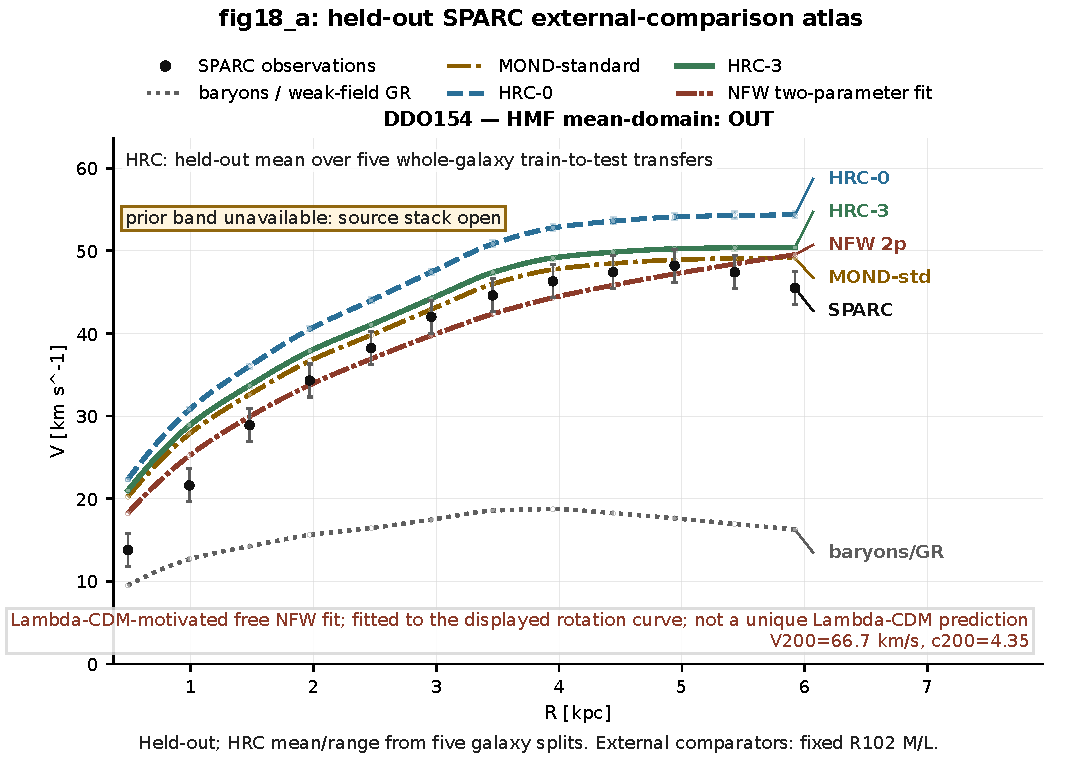
\includegraphics[width=1.14\textwidth]{figures/r154/curve_semantics/atlas/fig18_a_ddo154_r154.pdf}}
\caption{Held-out rotation-curve comparisons: DDO~154.  Points are SPARC
velocities; directly labelled curves show baryon-only weak-field GR,
MOND-standard, HRC-0, conditional HRC-3 and a separately fitted
two-parameter NFW halo.  The galaxies and whole-galaxy split assignment were
frozen before this rendering pass.  The calculation is a local algebraic
disk diagnostic, not a finite-thickness field solution or population
likelihood.  The NFW curve is $\Lambda$CDM-motivated and is not a unique
$\Lambda$CDM prediction.  The HRC centre is the pointwise mean of five held-out split
predictions at the tabulated radii; the split ranges are unconnected
per-radius whiskers, not a smoothed envelope.}
\label{fig:r123_atlas_f18a}
\label{fig:sparc_sample_new}
\end{figure}
\vspace*{\fill}
\RAtlasWideSingle{figures/r154/curve_semantics/atlas/fig18_b_ngc2403_r154.pdf}{fig:r123_atlas_f18b}{Held-out comparison: NGC~2403}{fig:sparc_external_model_comparison_r123_a}{held-out Level-C external comparison; not population model selection}
\RAtlasWideSingle{figures/r154/curve_semantics/atlas/fig18_c_ngc3198_r154.pdf}{fig:r123_atlas_f18c}{Held-out comparison: NGC~3198}{fig:sparc_external_model_comparison_r123_b}{held-out Level-C external comparison; not population model selection}
\RAtlasSingle{figures/r154/curve_semantics/atlas/fig18_d_ngc6503_r154.pdf}{fig:r123_atlas_f18d}{Held-out comparison: NGC~6503}{fig:sparc_external_model_comparison_r123_b}{held-out Level-C external comparison; not population model selection}
\clearpage
\begin{figure}[p]
\centering
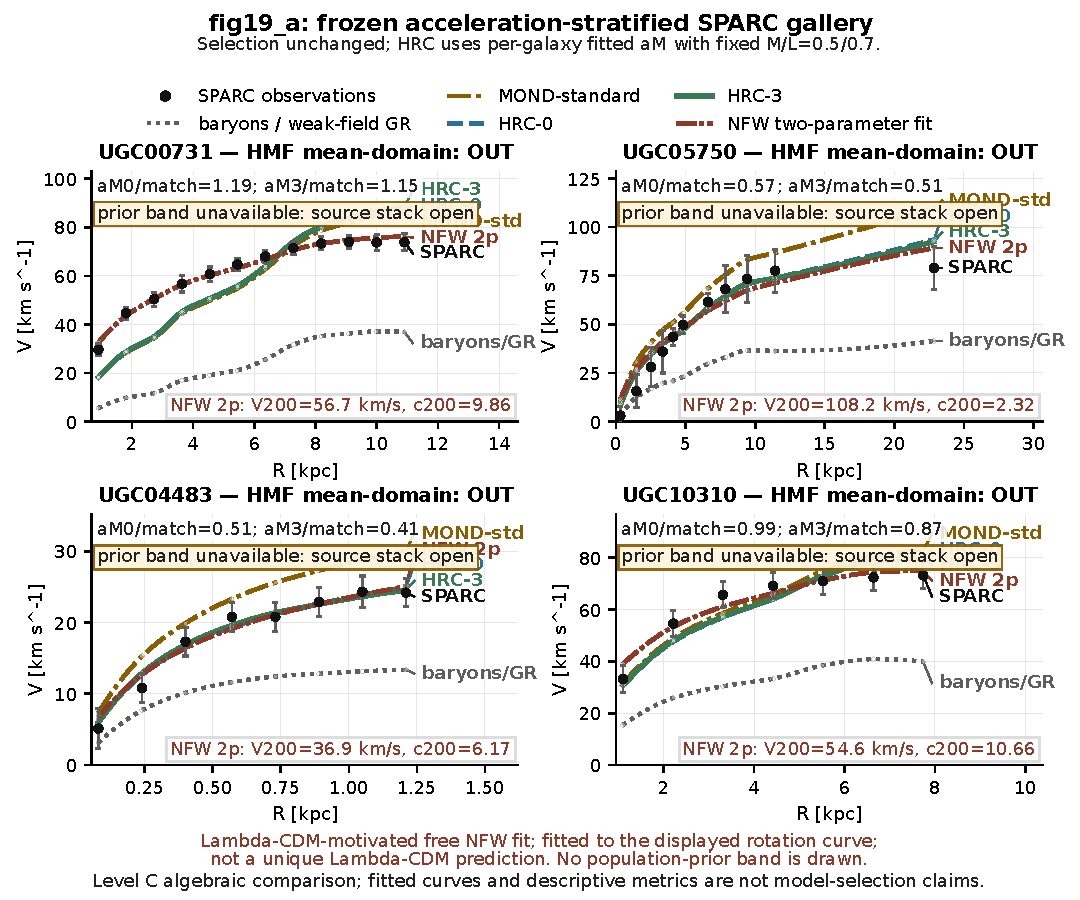
\includegraphics[width=\textwidth,height=0.76\textheight,keepaspectratio]{figures/r154/curve_semantics/atlas/fig19_a_gallery_lowacc_1_r154.pdf}
\caption{Frozen acceleration-stratified rotation-curve gallery.  Selection is
frozen without visual tuning: four quantiles are taken from each of four
strata in median baryonic acceleration.  Each panel shows SPARC data,
baryon-only weak-field GR, MOND-standard, HRC-0, conditional HRC-3 and a
separately fitted two-parameter NFW benchmark.  Per-galaxy fitted response
scales and NFW parameters make this a Level-C shape/residual diagnostic, not
a universal-scale or population model-selection result.  Smooth traces are display-only approximations through
residual-gated display nodes; source ordinates remain faint and unconnected,
and all metrics retain the original nodes.}
\label{fig:r123_atlas_f19a}
\label{fig:sparc_gallery_hrc}
\end{figure}
\FloatBarrier
\RAtlasSingle{figures/r154/curve_semantics/atlas/fig19_b_gallery_lowacc_2_r154.pdf}{fig:r123_atlas_f19b}{Frozen comparison gallery, low-acceleration page II}{fig:sparc_gallery_hrc}{frozen Level-C external comparison; not population model selection}
\RAtlasSingle{figures/r154/curve_semantics/atlas/fig19_c_gallery_highacc_1_r154.pdf}{fig:r123_atlas_f19c}{Frozen comparison gallery, high-acceleration page I}{fig:sparc_gallery_hrc}{frozen Level-C external comparison; not population model selection}
\RAtlasSingle{figures/r154/curve_semantics/atlas/fig19_d_gallery_highacc_2_r154.pdf}{fig:r123_atlas_f19d}{Frozen comparison gallery, high-acceleration page II}{fig:sparc_gallery_hrc}{frozen Level-C external comparison; not population model selection}
\clearpage
\begin{figure}[p]
\centering
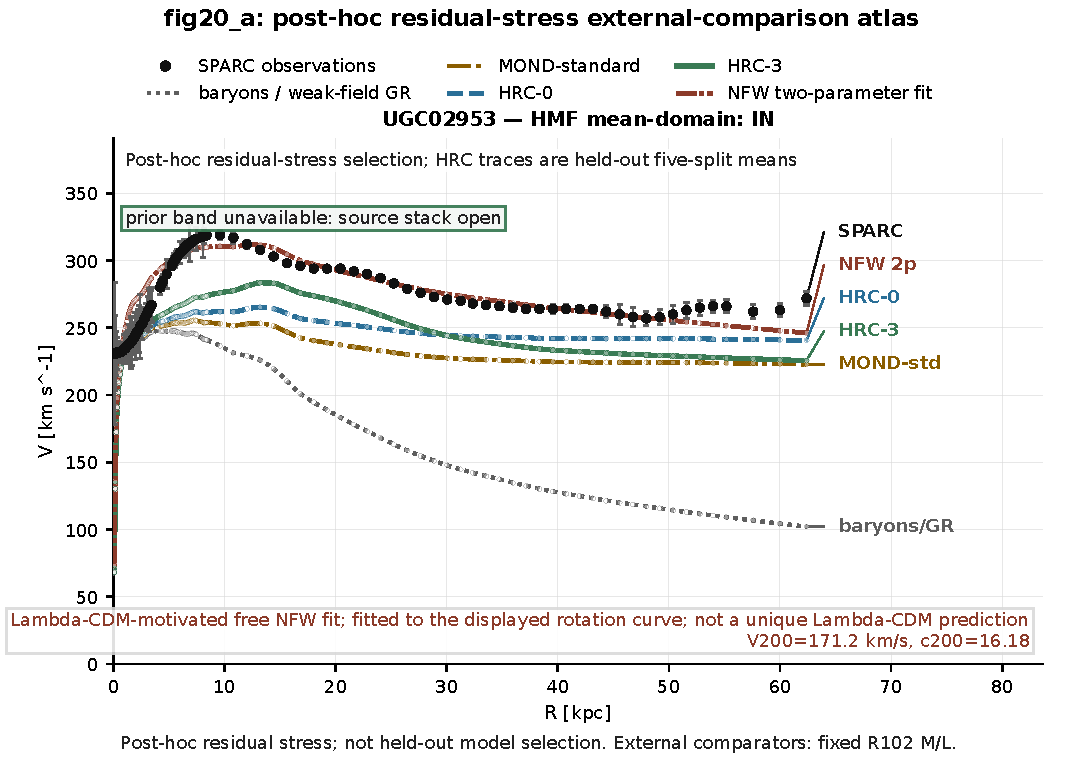
\includegraphics[width=\textwidth,height=0.76\textheight,keepaspectratio]{figures/r154/curve_semantics/atlas/fig20_a_ugc02953_r154.pdf}
\caption{Post-hoc residual-stress comparisons.  Two systems maximise the
HRC-0 minus HRC-3 fit difference and two maximise the reverse difference in
the frozen point registry.  Every panel now includes SPARC data, baryon-only
weak-field GR, MOND-standard, HRC-0, conditional HRC-3 and a separately
fitted two-parameter NFW benchmark.  Because the objects were selected after
viewing the residual statistic, this remains an explanatory Level-C red-team
diagnostic, not a held-out model-selection result.  Model traces use residual-gated, shape-preserving display
approximations through curvature-regularised display nodes; source ordinates
remain faint and unconnected and all metrics use the original nodes.}
\label{fig:r123_atlas_f20a}
\label{fig:hrc_residual_stress}
\end{figure}
\FloatBarrier
\RAtlasPair{0.932}{%
\RAtlasPanelUnit{figures/r154/curve_semantics/atlas/fig20_b_ugc09133_r154.pdf}{fig:r123_atlas_f20b}{Post-hoc residual stress: UGC~09133}{fig:hrc_residual_stress}{Level-C red-team diagnostic}}{%
\RAtlasPanelUnit{figures/r154/curve_semantics/atlas/fig20_c_ngc6946_r154.pdf}{fig:r123_atlas_f20c}{Post-hoc residual stress: NGC~6946}{fig:hrc_residual_stress}{Level-C red-team diagnostic}}
\RAtlasSingle{figures/r154/curve_semantics/atlas/fig20_d_ngc7331_r154.pdf}{fig:r123_atlas_f20d}{Post-hoc residual stress: NGC~7331}{fig:hrc_residual_stress}{Level-C red-team diagnostic}
\clearpage
\begin{figure}[p]
\centering
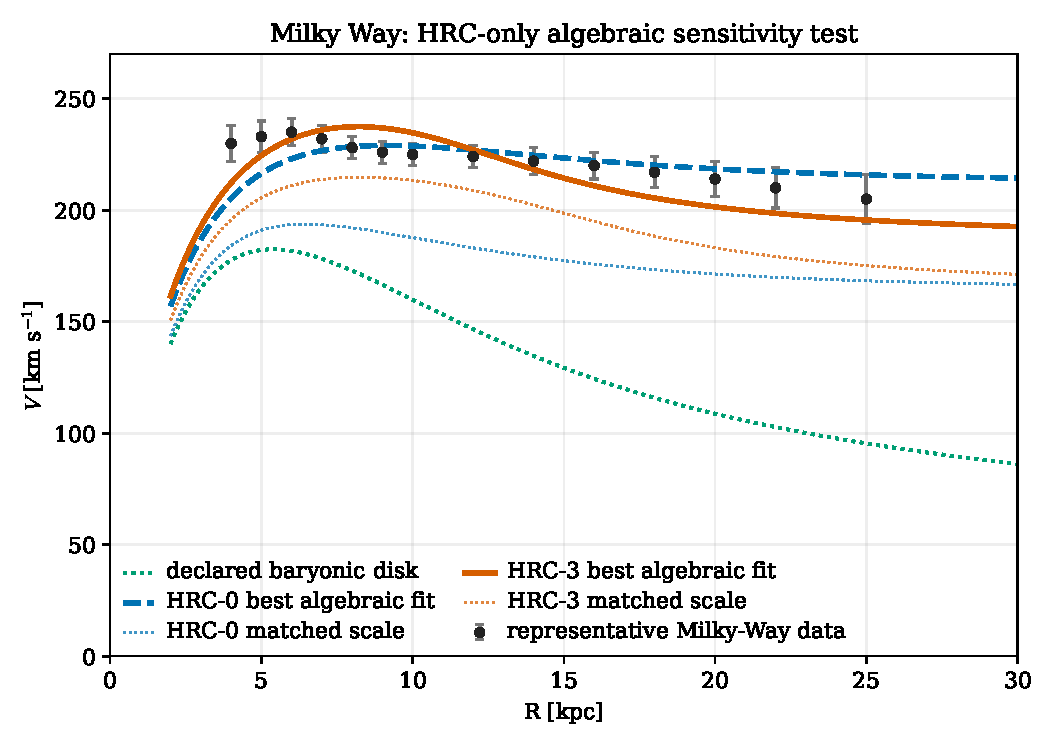
\includegraphics[width=\textwidth,height=0.76\textheight,keepaspectratio]{figures/r123/global/panels/fig_milky_way_hrc_only_r123.pdf}
\caption{Representative Milky-Way HRC sensitivity test.  Dotted HRC curves
use the matched scale; solid/dashed curves use the algebraic best-fit scale
for the declared exponential disk.  The figure does not replace a full
axisymmetric baryonic posterior.  The curve is relocated here as readable provenance
so that no HRC-only galaxy rotation plot remains a main-text model-comparison
owner.}
\label{fig:mw_new}
\end{figure}
\FloatBarrier
\clearpage
\section[\texorpdfstring{\protect\hspace{0.75em}Visual atlas: strong-field benchmarks}{Visual atlas: strong-field benchmarks}]{Visual atlas: strong-field benchmarks}
\label{app:r129_visual_strong_field}

The Tolman-kinematic and Hawking-temperature pages are retained as
external standard benchmarks.  They do not identify an ECT shell depth,
critical surface, physical Hilbert-space split or information-return law;
the ECT completion remains Open.

\RAtlasFirstSingle{figures/r154/curve_semantics/nonrotation/fig35_a_tolman_kinematics_smooth_r154.pdf}{fig:r123_atlas_f35a}{Tolman kinematic benchmark}{fig:bh_information}{external standard benchmark; \textit{Display semantics: }\detokenize{The smooth line is the densely evaluated exact external Tolman relation, not a fit to sampled data.}}
\RAtlasSingle{figures/r154/curve_semantics/nonrotation/fig35_c_hawking_benchmark_smooth_r154.pdf}{fig:r123_atlas_f35c}{Hawking benchmark}{fig:bh_information}{standard benchmark; ECT completion Open; \textit{Display semantics: }\detokenize{The smooth line is the densely evaluated exact external Hawking benchmark, not a fit to sampled data.}}
\clearpage
\section[\texorpdfstring{\protect\hspace{0.75em}Visual atlas: orientation and tensor bridge}{Visual atlas: orientation and tensor bridge}]{Visual atlas: orientation and tensor bridge}
\label{app:r129_visual_orientation_tensor}

This page preserves the conditional upstream orientation-stiffness
relation.  The continuation from that coefficient to a physical tensor
normalisation remains an Open ownership bridge.

\RAtlasFirstSingle{figures/r149/fig41_a_orientation_stiffness_upstream_r149.pdf}{fig:r123_atlas_f41a}{Upstream orientation stiffness}{fig:r103_Cn_scalechain_corrected}{conditional upstream relation; tensor bridge Open}
\clearpage
\section[\texorpdfstring{\protect\hspace{0.75em}Visual atlas: conditional background and cosmology}{Visual atlas: conditional background and cosmology}]{Visual atlas: conditional background and cosmology}
\label{app:r129_visual_background_cosmology}

These panels retain the named supplied expansion, distance and
kinematic-$w$ diagnostics, calibrated family and explicit scope statement.
They remain outputs of the conditional supplied state and do not constitute
a unique P1--P6 cosmology or a completed observable likelihood.  Continuous
traces are evaluated from the frozen dense background owner (with distance
obtained by deterministic quadrature); the eight or nine published diagnostic
nodes, as applicable, are shown separately.

\RAtlasFirstSingle{figures/r154/curve_semantics/nonrotation/fig42_a_named_expansion_dense_r154.pdf}{fig:r123_atlas_f42a}{Named supplied expansion}{fig:r103_ect_background_clocks}{conditional supplied background; \textit{Display semantics: }\detokenize{The continuous expansion trace is evaluated on the frozen 3001-point background owner; the nine published nodes are shown separately.}}
\RAtlasSingle{figures/r154/curve_semantics/nonrotation/fig42_c_comoving_distance_dense_r154.pdf}{fig:r123_atlas_f42c}{Comoving-distance diagnostic}{fig:r103_ect_background_clocks}{conditional supplied background; \textit{Display semantics: }\detokenize{The continuous distance trace is obtained by deterministic quadrature of the frozen dense background; the eight nonzero-z published nodes are shown separately.}}
\RAtlasPair{0.817}{%
\RAtlasPanelUnit{figures/r154/curve_semantics/nonrotation/fig42_d_background_w_dense_r154.pdf}{fig:r123_atlas_f42d}{Background equation-of-state proxy}{fig:r103_ect_background_clocks}{conditional supplied background; \textit{Display semantics: }\detokenize{Both continuous effective-equation-of-state traces are evaluated on the frozen dense background and declared matched control; the nine published nodes are shown separately.}}}{%
\RAtlasPanelUnit{figures/r123/global/panels/fig42_e_calibrated_family_r123.pdf}{fig:r123_atlas_f42e}{Calibrated background family}{fig:r103_ect_background_clocks}{Level-C conditional family}}
\RAtlasSingle{figures/r123/global/panels/fig42_f_scope_statement_r123.pdf}{fig:r123_atlas_f42f}{Background scope and ownership}{fig:r103_ect_background_clocks}{explicit Open-owner statement}
\RAtlasSingle{figures/r154/curve_semantics/nonrotation/fig43_b_two_slope_w_dense_r154.pdf}{fig:r123_atlas_f43b}{Two-slope $w$ diagnostic}{fig:r103_two_slope_HwG_conditional}{conditional supplied background; \textit{Display semantics: }\detokenize{Both continuous effective-equation-of-state traces are evaluated on the frozen dense background and declared matched control; the nine published nodes are shown separately.}}
\clearpage
\section[\texorpdfstring{\protect\hspace{0.75em}Visual atlas: finite-body scalar gates}{Visual atlas: finite-body scalar gates}]{Visual atlas: finite-body scalar gates}
\label{app:r129_visual_finite_body_scalar}

The retained tail-estimator page is fixed-metric numerical detail for
the named scalar boundary-value diagnostic.  It is not a coupled metric body
solution, Cassini likelihood, WEP result or full-PPN pass.

\RAtlasFirstSingle{figures/r123/global/panels/fig45_b_tail_estimators_r123.pdf}{fig:r123_atlas_f45b}{Finite-body tail estimators}{fig:r114_finitebody_scalar_gates}{fixed-metric numerical detail; not a PPN pass}

\clearpage
\noindent
This atlas records visual preservation and the outcome of exact-page
readability gates only.  It does not
close any Open action, state, metric, likelihood or experimental-owner gate
identified by the corresponding main-text section.
\section*{Data and Code Availability}
\addcontentsline{toc}{part}{Data and Code Availability}

Galaxy rotation-curve data are drawn from the public SPARC database \cite{Lelli2016}
(\url{http://astroweb.cwru.edu/SPARC/}).  Versioned source and reproducibility
materials for released revisions are available at:

\begin{center}
  \url{https://github.com/chufelo/ECT-preprint-code}
\end{center}

\noindent
For an exact revision, use the tagged commit and frozen release manifest
associated with its version-specific DOI.  The moving default branch may later
change and is not an exact citation owner.

\noindent
The versioned validation package contains the P6 record-sector scripts
for kernel-exponent, threshold-residue, sum-rule and M3 guard checks, together
with the synthetic two-parameter-family P26 over-closure demonstration.
It also contains the exact conditional two-slope cosmology equations,
dual-integrator background and
ordered-branch clock outputs, restricted growth/Weyl/flow diagnostics, and
the owner/identifiability gates.  These are conditional outputs of the
declared action and state, not a unique P1--P6 cosmology or a full Hubble,
JWST, lensing or growth likelihood.  A physical numerical release must retain
the continuous exact-action protocol of
Appendix~\ref{app:late_cosmo_algorithm} and must freeze every action, state,
boundary datum and observable likelihood.

\noindent
The same versioned package contains the HRC-0 analytic inversion,
deterministic residual-checked HRC-3 solvers, signed-gas handling, the
165-galaxy HRC catalogue, fixed/free $M/L$ sensitivity, representative
Milky-Way and UDG stress tests, all nine HRC figures, and machine-readable
verification outputs.  The frozen HRC layer does not claim a finite-thickness
disk PDE, covariance-complete likelihood or metric/lensing completion.  The
main narrative adds a separately frozen, qualified six-galaxy comparison with
MOND-standard and a fitted two-parameter NFW halo benchmark.  This is a
Level-C algebraic diagnostic; NFW is $\Lambda$CDM-motivated and is not a
unique $\Lambda$CDM prediction.  The package also contains the action-scale,
fifth-force, baryogenesis, dimensionality and P6 verification calculations
described in their owning sections.  The release manifest identifies the exact
files and hashes belonging to a published revision.

The computational procedures used to generate the individual figures
are summarised in Appendix~\ref{app:algorithms}.

\medskip
\noindent
\begin{minipage}{0.72\linewidth}
  The public repository can also be accessed by scanning the QR code
  (right).  Original project code is MIT-licensed under the repository's
  declared licence scope; third-party data and assets retain their own terms.
  Each exact release is identified there by its tagged commit and frozen
  manifest.
\end{minipage}
\hfill
\begin{minipage}{0.22\linewidth}
  \centering
  
\includegraphics[width=\linewidth]{figures/github_qr.png}
  \scriptsize\texttt{github.com/chufelo/\\ECT-preprint-code}
\end{minipage}

\section*{Acknowledgments}
\addcontentsline{toc}{part}{Acknowledgments}
The author thanks T.~Jacobson for drawing attention to the closely
related clock-field construction of Mukohyama and Uzan, which helped
sharpen the comparative positioning of the present work.
The author thanks the open-source scientific community for the SPARC galaxy database
and the publicly available tools used in this work.
The author declares no competing interests and received no external funding for this research.


\bibliographystyle{unsrt}

\phantomsection
\addcontentsline{toc}{part}{References}

\bibliography{references}


\end{document}
